%% This is the ctufit-thesis example file. It is used to produce theses
%% for submission to Czech Technical University, Faculty of Information Technology.
%%
%% Get the newest version from
%% https://gitlab.fit.cvut.cz/theses-templates/FITthesis-LaTeX

% arara: xelatex
% arara: biber
% arara: xelatex
% arara: xelatex

%%%%%%%%%%%%%%%%%%%%%%%%%%%%%%%%%%%%%%%%%
% CLASS OPTIONS
% language: czech/english/slovak
% thesis type: bachelor/master/dissertation
% electronic (oneside) or printed (twoside), twoside is default
% paragraph - if passed, this optional argument sets paragraphs as the deepest level of headers, styles it, numbers it and adds it to Table of Content. Use with care! Normally, it is considered unwise to use it, since it is too deep.
% colour: bw for black&white OR no option for default colour scheme. If used, this must be the LAST option!
%%%%%%%%%%%%%%%%%%%%%%%%%%%%%%%%%%%%%%%%%
\documentclass[english,bachelor,unicode,oneside,bw]{ctufit-thesis}

%%%%%%%%%%%%%%%%%%%%%%%%%%%%%%%%%%
% FILL IN THIS INFORMATION
%%%%%%%%%%%%%%%%%%%%%%%%%%%%%%%%%%
\ctufitauthorsurnames{Laštovička}
\ctufittitle{NAC-colorings search: complexity and algorithms}
\ctufitauthorfull{Petr Laštovička}
\ctufitauthorgivennames{Petr}
\ctufitsupervisor{Dr.\,techn.\,Ing.\,Jan Legerský}
\ctufitdepartment{Department of Theoretical Computer Science}
\ctufitprogram{Informatics}
\ctufitspecialisation{Computer Science}
\ctufityear{2025}
\ctufitdeclarationplace{Prague}
\ctufitdeclarationdate{\today} % replace with the date of signature of the declaration
\ctufitabstractCZE{
    Jednou z otázek v strukturální teorii tuhosti (Rigidity Theory)
    je, zda realizace vrcholů grafu do roviny je pohyblivá,
    tj.~zda umožňuje spojitou deformaci neměnící délku hran.
    %
    Pohyblivá realizace souvislého grafu v rovině existuje právě tehdy, když
    graf má NAC-obarvení, což je hranové obarvení dvěma barvami takové,
    že pro každý cyklus jsou všechny hrany obarveny stejnou barvou nebo
    jsou každou barvou obarveny alespoň dvě hrany.
    %
    Je NP-úplné rozhodnout, zda graf má NAC-obarvení, v práci ukazujeme,
    že problém je NP-úplný i pro grafy s maximálním stupněm pět.
    %
    Představujeme značně rychlejší algoritmus na hledání NAC-obarvení společně s různými heuristikami.
    Srovnáváme ho s předchozími algoritmy a porovnáváme i heuristiky mezi sebou.
    %
    Následně představujeme FPT algoritmus na počítání NAC-obarvení
    parametrizovaný stromovou šířkou.
    %
    % Navíc popisujeme vztahy s stable řezy grafu a implementujeme algoritmus
    % pro jejich hledání v flexible grafech.
}
% Also update README.md if any changes are made.
\ctufitabstractENG{
    One of the questions in Rigidity Theory is whether a realization of the
    vertices of a graph in the plane is flexible, namely, if it allows a continuous
    deformation preserving the edge lengths.
    %
    A flexible realization of a connected graph in the plane exists if and only if
    the graph has a NAC-coloring, which is surjective edge coloring by
    two colors such that for each cycle either all the edges have the same color or
    there are at least two edges of each color.
    %
    While it is known that it is \mbox{NP-complete}
    to decide if a graph has a NAC-coloring,
    we show that the problem is
    also NP-complete for graphs with maximum degree five.
    %
    We present a significantly faster algorithm implementation for NAC-coloring search,
    and we discuss related heuristics.
    The performance is compared with previous algorithms and among the heuristics.
    %
    We also present fixed-parameter tractable (FPT) algorithm for NAC-coloring counting
    parametrized by tree width.
    %
    % We also discuss relation to stable cuts and algorithm for finding
    % a stable cut is implemented as part of the thesis.
}

\ctufitkeywordsCZE{
    strukturální teorie tuhosti,
    generická flexibilita,
    NAC-obar\-vení,
    stable-cut,
    parametrizovaná komplexita,
    NP-úplnost
}
\ctufitkeywordsENG{
    rigidity theory,
    generic flexibility,
    NAC-coloring,
    stable-cut,
    \newline
    parametrized complexity,
    NP-completeness
}
%%%%%%%%%%%%%%%%%%%%%%%%%%%%%%%%%%
% END FILL IN
%%%%%%%%%%%%%%%%%%%%%%%%%%%%%%%%%%

%%%%%%%%%%%%%%%%%%%%%%%%%%%%%%%%%%
% CUSTOMIZATION of this template
% Skip this part or alter it if you know what you are doing.
%%%%%%%%%%%%%%%%%%%%%%%%%%%%%%%%%%

\RequirePackage{iftex}[2020/03/06]
\iftutex{}% XeLaTeX and LuaLaTeX
    \RequirePackage{ellipsis}[2020/05/22] %ellipsis workaround for XeLaTeX
\else
    \errmessage{Only compilation with XeLaTeX or LuaLaTeX is allowed}
    \stop
\fi

% hyperlinks
\hypersetup{
    pdfpagelayout=TwoPageRight,
    colorlinks=false,
    allcolors=decoration,
    pdfborder={0 0 0.1}
}

% uncomment the following to hide all hyperlinks
%\hypersetup{hidelinks}

% uncomment the following to change the color of all hyperlinks to CTU blue
\hypersetup{allbordercolors=decoration}

\RequirePackage{pdfpages}[2020/01/28]

%%%%%%%%%%%%%%%%%%%%%%%%%%%%%%%%%%
% CUSTOMIZATION of this template END
%%%%%%%%%%%%%%%%%%%%%%%%%%%%%%%%%%


%%%%%%%%%%%%%%%%%%%%%%
% CONTENTS SETTINGS
%%%%%%%%%%%%%%%%%%%%%%
\usepackage{dirtree}
\usepackage{lipsum,tikz}
\usepackage{xurl}
\usepackage{listings} % typesetting of sources
%\usepackage{minted}
\usepackage{csquotes}
% Handles czech line breaks
% \usepackage{xevlna}
% Should improve line breaking
\usepackage{microtype}
\usepackage{pdflscape}
\usepackage{hyperref}
\usepackage[nameinlink]{cleveref}
\usepackage{todonotes}

\usepackage{algorithm}
\usepackage{algorithmicx}
\usepackage{algpseudocode}

\usepackage[style=iso-numeric]{biblatex}
\addbibresource{./text/bib-database.bib}
%%%%%%%%%%%%%%%%%%%%%%
% CONTENTS SETTINGS END
%%%%%%%%%%%%%%%%%%%%%%

%%%%%%%%%%%%%%%%%
% CUSTOM COMMANDS
%%%%%%%%%%%%%%%%%

% Text mode macros
\newcommand{\G}{\(G\)}
\newcommand{\Ered}{E_\text{red}}
\newcommand{\Eblue}{E_\text{blue}}
%% Proof, Algo
\newcommand{\true}{\textit{True}}
\newcommand{\false}{\textit{False}}
\DeclareMathOperator{\CP}{\Pi_{\NAC}}
\DeclareMathOperator{\partition}{\mathbf{partition}}
\DeclareMathOperator{\cycle}{\mathbf{cycle}}
\DeclareMathOperator{\NACcond}{\mathbf{NACcond}}

\newcommand{\Naive}{\textsc{Naive}}
\newcommand{\NaiveCycles}{\textsc{NaiveCycles}}
\newcommand{\Subgraphs}{\textsc{Subgraphs}}
\newcommand{\None}{\textsc{None}}
\newcommand{\Neighbors}{\textsc{Neighbors}}
\newcommand{\NeighborsDegree}{\textsc{NeighborsDegree}}
\newcommand{\CyclesMatchChunks}{\textsc{CyclesMatchChunks}}
\newcommand{\KernighanLin}{\textsc{Kernighan-Lin}}
\newcommand{\Cuts}{\textsc{Cuts}}
\newcommand{\CycleMask}{\textsc{CycleMask}}
\newcommand{\IsNACColoring}{\textsc{IsNACColoring}}
\newcommand{\MergeLinear}{\textsc{Linear}}
\newcommand{\SharedVertices}{\textsc{SharedVertices}}
\newcommand{\Log}{\textsc{Log}}
\newcommand{\MinMax}{\textsc{MinMax}}
\newcommand{\PromisingCycles}{\textsc{PromisingCycles}}
\newcommand{\Score}{\textsc{Score}}
%% FPT
\newcommand{\MSO}{$\text{MSO}_2$}
\newcommand{\Xt}{\(X_t\)}
\newcommand{\LeafNode}{\textsc{Leaf Node}}
\newcommand{\RootNode}{\textsc{Root Node}}
\newcommand{\IntroduceVertexNode}{\textsc{Introduce Vertex Node}}
\newcommand{\ForgetVertexNode}{\textsc{Forget Vertex Node}}
\newcommand{\IntroduceEdgeNode}{\textsc{Introduce Edge Node}}
\newcommand{\JoinNode}{\textsc{Join Node}}
\newcommand{\IntroduceVertexWithEdgesNode}{\textsc{Introduce Vertex With Edges Node}}

\newcommand{\flexrilog}{\textsc{FlexRiLoG}}
\newcommand{\trcon}{$\triangle$-connected}

% Math mode macros
\newcommand{\red}{\text{red}}
\newcommand{\blue}{\text{blue}}
\DeclareMathOperator{\NAC}{NAC}
\newcommand{\nac}[1]{\NAC(#1)}
\newcommand{\nnac}[1]{\NAC_{\#} (#1)}
\newcommand{\N}{\mathbb{N}}
\newcommand{\R}{\mathbb{R}}
\newcommand{\inc}{\text{inc}}
\newcommand{\pluseq}{\mathrel{+}=}
\newcommand{\equivclass}[2]{%
  #1{/\!}_{#2}%
}
%% Stable cuts
\newcommand{\GSC}{\mathcal{G}_{sc}}
%% Bitwise operators
\newcommand*\BitAnd{\mathbin{\&}}
\newcommand*\BitOr{\mathbin{|}}
\newcommand*\ShiftLeft{\ll}
\newcommand*\ShiftRight{\gg}
\newcommand*\BitNeg{\ensuremath{\mathord{\sim}}}


%%%%%%%%%%%%%%%
\colorlet{ecol}{black!50!white}
\definecolor{colR}{rgb}{.932,.172,.172} %x11 Firebrick2
\definecolor{colB}{rgb}{.255,.41,.884} %svgnames RoyalBlue
\definecolor{colOrange}{RGB}{255,191,0} %Amber
%% Tikz styles
\tikzstyle{vertex}=[circle, draw, fill=black, inner sep=0pt, minimum size=4pt]
\tikzstyle{vertexSig}=[circle, draw, fill=colOrange, inner sep=0pt, minimum size=4pt]
\tikzstyle{edge}=[line width=1.5pt,ecol]
% dotted, densely dotted, loosely dotted, dashed
\tikzstyle{dots}=[dotted dash=1.5pt]
\tikzstyle{redge}=[edge,colR]
\tikzstyle{bedge}=[edge,colB]
\tikzstyle{yedge}=[edge,colOrange]

%%%%%%%%%%%%%%%%%
\renewcommand{\algorithmicrequire}{\textbf{Input:}}
\renewcommand{\algorithmicensure}{\textbf{Output:}}
\newcommand{\Break}{\State \textbf{break} }
\newcommand{\Continue}{\State \textbf{continue} }
\newcommand{\union}[1]{\textsc{union} ($#1$)}

%%%%%%%%%%%%%%%%%
% MatPlotlib graphs
% colors bright form https://personal.sron.nl/~pault/#sec:qualitative
\definecolor{currentstroke1}{HTML}{BBBBBB}
\definecolor{currentstroke2}{HTML}{EE6677}
\definecolor{currentstroke3}{HTML}{228833}
\definecolor{currentstroke4}{HTML}{CCBB44}
\definecolor{currentstroke5}{HTML}{66CCEE}
\definecolor{currentstroke6}{HTML}{AA3377}
\definecolor{currentstroke7}{HTML}{4477AA}
% Required for some Matplotlib (3.9.*) exported graphs to render as
% its pgd export feature is broken
% https://github.com/matplotlib/matplotlib/issues/27907
\providecommand\mathdefault[1]{#1}

%%%%%%%%%%%%%%%%%
% CUSTOM COMMANDS END
%%%%%%%%%%%%%%%%%


\begin{document}
\frontmatter\frontmatterinit{} % do not remove these two commands

\thispagestyle{empty}\maketitle\thispagestyle{empty}\cleardoublepage{} % do not remove these four commands

% 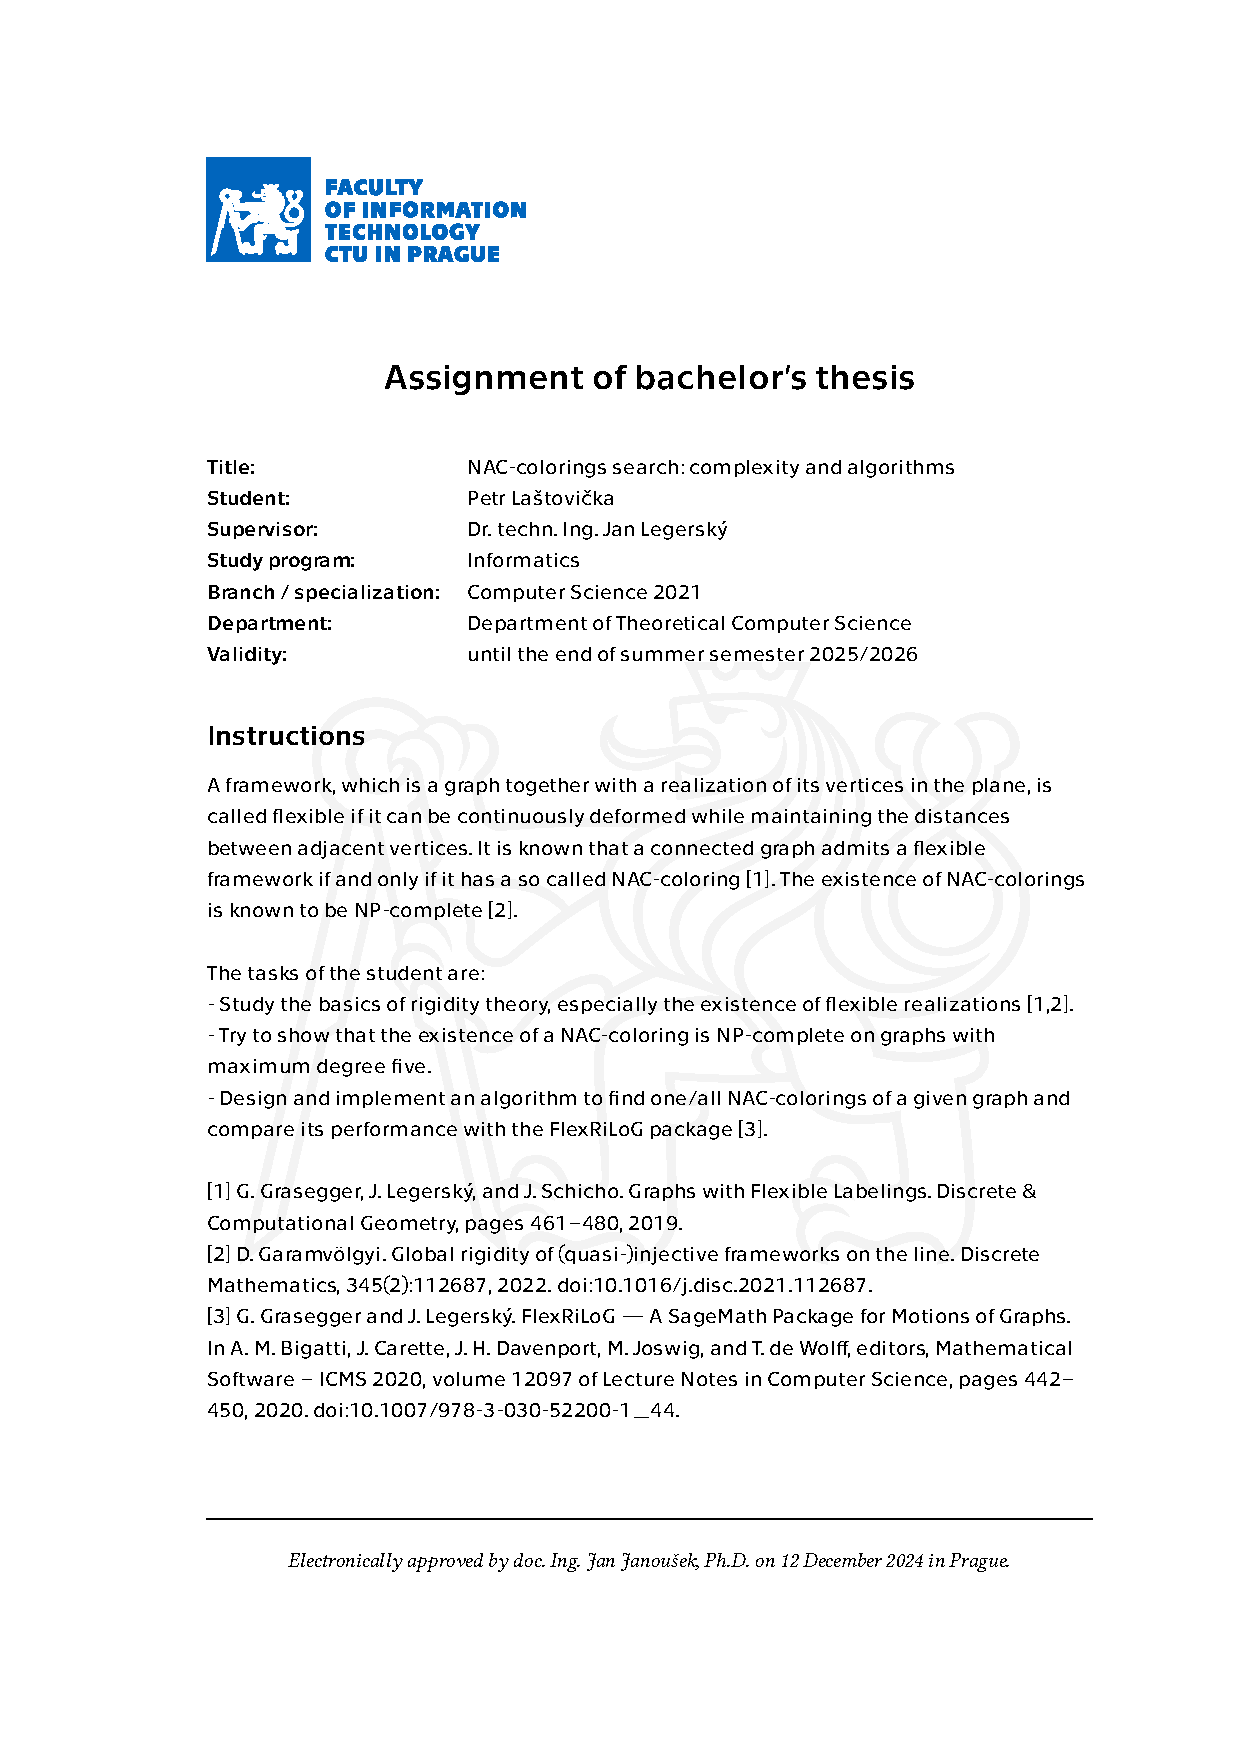
\includepdf[pages={1-}]{./assets/assignment_projects.pdf} % thesis assignment generated from ProjectsFIT, or KOS, nooooo
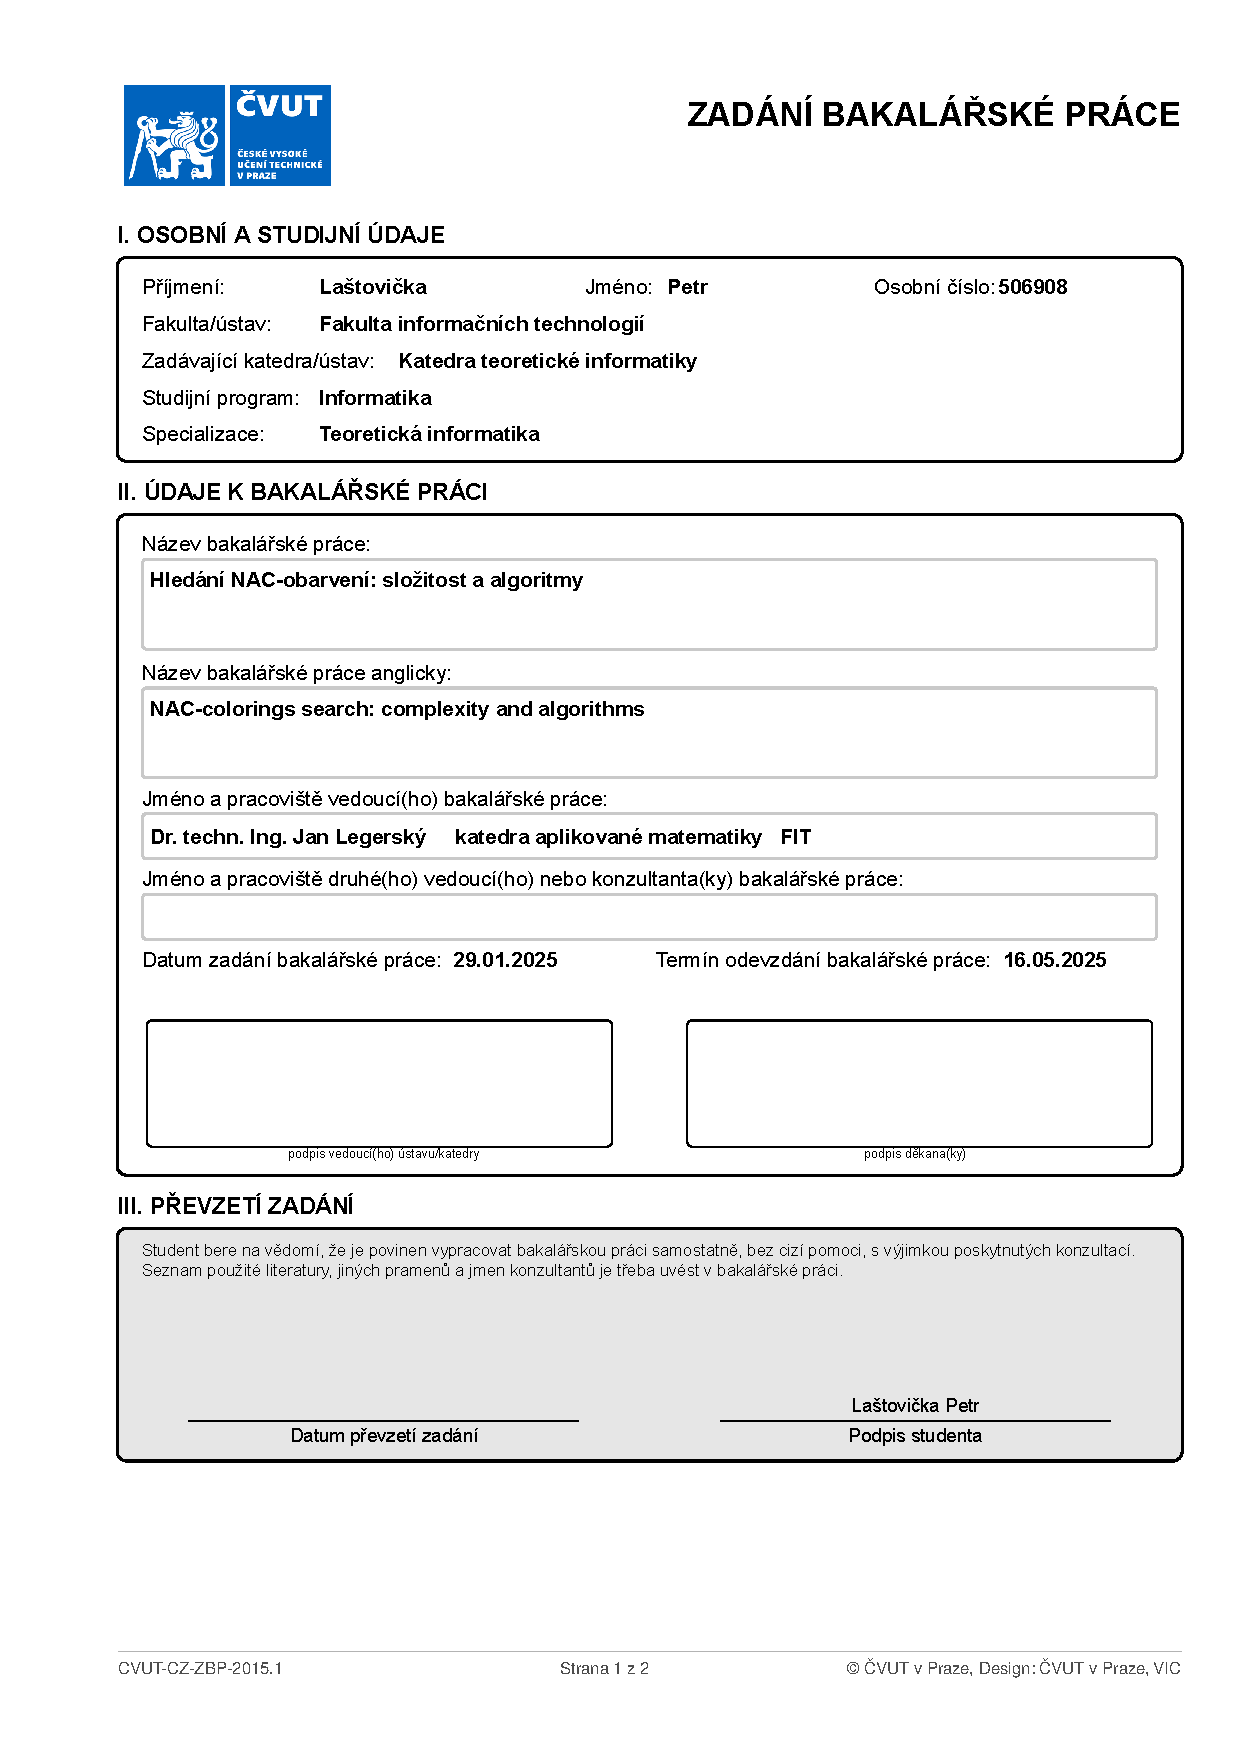
\includepdf[pages={1-}]{./assets/assignment_kos.pdf} % thesis assignment generated from ProjectsFIT, or KOS, nooooo

\imprintpage{} % do not remove this command
\stopTOCentries{} % This should not be removed!

%%%%%%%%%%%%%%%%%%%%%%
% list of other contents END
%%%%%%%%%%%%%%%%%%%%%%

%%%%%%%%%%%%%%%%%%%
% ACKNOWLEDGMENT
% This is a place to thank people for helping you. It is common to thank your supervisor.
%%%%%%%%%%%%%%%%%%%
\begin{acknowledgmentpage}
	Chtěl bych poděkovat především sit amet, consectetuer adipiscing elit. Curabitur sagittis hendrerit ante. Class aptent taciti sociosqu ad litora torquent per conubia nostra, per inceptos hymenaeos. Cras pede libero, dapibus nec, pretium sit amet, tempor quis. Sed vel lectus. Donec odio tempus molestie, porttitor ut, iaculis quis, sem. Suspendisse sagittis ultrices augue.

	Vedoucí
	Michal Opler za nápad FTP
	Knop za materiály
	Rodina
	Přátelé
	Učitelům KTI a KAM
\end{acknowledgmentpage}
%%%%%%%%%%%%%%%%%%%
% ACKNOWLEDGMENT END
%%%%%%%%%%%%%%%%%%%


%%%%%%%%%%%%%%%%%%%
% DECLARATION
% FILL IN / MODIFY
%%%%%%%%%%%%%%%%%%%
% INSTRUCTIONS
% https://courses.fit.cvut.cz/SFE/download/index.html#_documents () (prohlášení do ZP)
\begin{declarationpage}
	I hereby declare that the presented thesis is my own work and that I have cited all sources of
	information in accordance with the Guideline for adhering to ethical principles when elaborating an
	academic final thesis.

	I acknowledge that my thesis is subject to the rights and obligations stipulated by the Act No.
	121/2000 Coll., the Copyright Act, as amended. In accordance with Section 2373(2) of Act No.
	89/2012 Coll., the Civil Code, as amended, I hereby grant a non-exclusive authorization (license) to
	utilize this thesis, including all computer programs that are part of it or attached to it and all
	documentation thereof (hereinafter collectively referred to as the ``Work''), to any and all persons
	who wish to use the Work. Such persons are entitled to use the Work in any manner that does not
	diminish the value of the Work and for any purpose (including use for profit). This authorization is
	unlimited in time, territory and quantity.

	I declare that I have used AI tools during the preparation and writing of my thesis. I have verified
	the generated content. I confirm that I am aware that I am fully responsible for the content of the
	thesis.
\end{declarationpage}
%%%%%%%%%%%%%%%%%%%
% DECLARATION END
%%%%%%%%%%%%%%%%%%%

\printabstractpage{} % do not remove this command

%%%%%%%%%%%%%%%%%%%
% SUMMARY
% FILL IN / MODIFY
% OR REMOVE ENTIRELY (upon agreement with your supervisor)
% (appropriate to remove in most theses)
%%%%%%%%%%%%%%%%%%%
% \begin{summarypage}
% \section*{Summary section}
% 
% \lipsum[1][1-8]
% 
% \section*{Summary section}
% 
% \lipsum[2][1-6]
% 
% \section*{Summary section}
% 
% \lipsum[3]
% 
% \section*{Summary section}
% 
% \lipsum[2]
% 
% \section*{Summary section}
% 
% \lipsum[1][1-8] Lorem lorem lorem.
% \end{summarypage}
%%%%%%%%%%%%%%%%%%%
% SUMMARY END
%%%%%%%%%%%%%%%%%%%

\tableofcontents % do not remove this command
%%%%%%%%%%%%%%%%%%%%%%
% list of other contents: figures, tables, code listings, algorithms, etc.
% add/remove commands accordingly
%%%%%%%%%%%%%%%%%%%%%%
\listoffigures % list of figures
\begingroup
\let\clearpage\relax
\listoftables % list of tables
% \thectufitlistingscommand{}
\thectufitlistofalgorithmscommand{}
\endgroup

%%%%%%%%%%%%%%%%%%%
% ABBREVIATIONS
% FILL IN / MODIFY
% OR REMOVE ENTIRELY
% List the abbreviations in lexicography order.
%%%%%%%%%%%%%%%%%%%
\chapter{\thectufitabbreviationlabel}

\begin{tabular}{rl}
	CNF                & Conjunctive normal form              \\
	CSV                & Comma-separated values               \\
	FPT                & Fixed-parameter tractable            \\
	\( \text{MSO}_2 \) & Monadic second-order logic on graphs \\
	NAC                & No almost cycles                     \\
	SAT                & Boolean satisfiability problem       \\
\end{tabular}
%%%%%%%%%%%%%%%%%%%
% ABBREVIATIONS END
%%%%%%%%%%%%%%%%%%%
\resumeTOCentries{}
\mainmatter\mainmatterinit{} % do not remove these two commands
%%%%%%%%%%%%%%%%%%%
% THE THESIS
% MODIFY ANYTHING BELOW THIS LINE
%%%%%%%%%%%%%%%%%%%

% \listoftodos{}\newpage{}


\chapter{Introduction}
% uncomment the following line to create an unnumbered chapter
%\chapter*{Introduction}\addcontentsline{toc}{chapter}{Introduction}\markboth{Introduction}{Introduction}
\setcounter{page}{1}

% Pohádka
% Nepřehánět to s definicemi a citacemi -> spíše teoretická část
% Proč to dělám, význam, návaznost (PyRigi)
% Jak jsem si to vybral
% prodat drony
% Cíle
% - část úvodu, nebo vlastní kapitola
% Obsah jen stručně

The core concept of Rigidity Theory is a \emph{framework} of a simple graph \(G\).
It is a realization of \(G\) into a \(d\)-dimensional plane \(p: V(G) \to \R^d\).
A framework is \emph{\( d \)-flexible} if there exists a transformation
that continuously translates some subset of vertices in such a way that
distances between neighboring vertices are preserved during the transformation.
Otherwise, the framework is called \emph{\( d \)-rigid}.

For \( d = 1 \) all the vertices are on a line
and any vertex deviation necessarily changes distances (if the graph is connected).
%
For \( d \ge 3 \) we can map all the vertices except one onto a line and
rotate the vertex around the line.
%
The interesting case is when \( d = 2 \) --- a mapping into a plane.
It is known that a graph has most of the realizations
either \( 2 \)-flexible, or \( 2 \)-rigid,
still there may be some realizations of the other type~\cite{generically_rigid_graphs}
--- we talk about paradoxical flexibility.
A graph is \emph{(generically) rigid} if most of the realizations are \( 2 \)-rigid
and \emph{(generically) flexible} if most of the realizations are \( 2 \)-flexible.

An example application of the Rigidity Theory is a squadron of drones
where the drones can measure distance to their close neighbors.
Can we determine the locations of all the drones
down to translation and rotation of the whole squadron
just from such information?

For similar problems in the plane,
one would think that if the graph formed is rigid, the answer is yes, and
for flexible graphs the answer is no.
But as stated above, paradoxically even a rigid graph can have a flexible realization,
and it may just happen that the drones form such a \( 2 \)-flexible framework.

In efforts to find such paradoxical realizations,
a new edge coloring was defined~\cite{legersky_original}.
A \emph{NAC-coloring} is an edge coloring of a graph by \( \red \) and \( \blue \)
such that both the colors are used and there is no almost cycle formed.
An \emph{almost cycle} is a cycle in the colored graph such that exactly one
edge of the cycle is colored \( \red \) or exactly one edge is colored \( \blue \).
Such coloring exists if and only if the graph has a flexible realization.
This provides a simple but strong tool to decide whenever a graph has
a flexible realization even if it is rigid.
As shown later in the thesis, one can check in polynomial time if a coloring
given is a NAC-coloring.
Unfortunately, it is NP-complete to decide if a graph has any NAC-coloring.

\begin{figure}[ht]
	\centering
	\begin{tikzpicture}[rotate=90,scale=1.5]
		\node[vertex] (a) at (0,0) {};
		\node[vertex] (b) at (1,0) {};
		\node[vertex] (c) at (0.5,0.5) {};
		\node[vertex] (d) at (0,1.5) {};
		\node[vertex] (e) at (1,1.5) {};
		\node[vertex] (f) at (0.5,1) {};
		\draw[bedge] (a)edge(b) (b)edge(c) (c)edge(a) (d)edge(e) (e)edge(f) (f)edge(d) ;
		\draw[redge] (a)edge(d) (b)edge(e) (c)edge(f);
	\end{tikzpicture}
	\qquad
	\qquad
	\begin{tikzpicture}[rotate=90,scale=1.5]
		\node[vertex] (a) at (0.00,0) {};
		\node[vertex] (b) at (1.00,0) {};
		\node[vertex] (c) at (0.50,0.5) {};
		\node[vertex] (d) at (0.25,1) {};
		\node[vertex] (e) at (1.25,1) {};
		\node[vertex] (f) at (0.75,1.5) {};
		\draw[edge] (a)edge(b) (b)edge(c) (c)edge(a) (d)edge(e) (e)edge(f) (f)edge(d) ;
		\draw[edge] (a)edge(d) (b)edge(e) (c)edge(f);
	\end{tikzpicture}
	\caption{The $3$-prism is generically $2$-rigid, but has a flexible realization (right).
		It has a unique NAC-coloring modulo swapping colors (left).}%
	\label{fig:3prism}
\end{figure}

A nice example for NAC-coloring showcase is the prism graph~\Cref{fig:3prism},
a graph formed from two triangles with three interconnecting edges.
Such graph is rigid, still it has a NAC-coloring and flexible realizations.
The flexible realizations are all the realization where
the triangles are identical except for translation.
You can check yourself that there are
no other NAC-colorings except the symmetric one.

The goals of this thesis are to provide an algorithm
that can find all the NAC-colorings of a graph.
Multiple heuristics will be used to significantly
reduce the runtime of the algorithm.
We also provide parametrized approach where complexity can be reduced for graphs
with low internal structural complexity (tree width).
We also show that the problem of deciding if a graph has a NAC-coloring
is NP-complete even on graphs with maximal degree five.
Later also show relation to stable cuts~\cite{stable_cuts_2v_4}.
Code implemented in this thesis will enrich the existing PyRigi~\cite{pyrigi}
library for Rigidity Theory.
Currently, there are no such algorithms implemented in PyRigi itself,
the only known implementation is rather naive in FlexRiLoG~\cite{flexrilog}.
We compare our implementation performance with FlexRiLoG and also compare
individual heuristics among each other.
Multiple relevant graph classes will be considered.

We summarize and extend our previous research done
on the topic in~\cite{my_paper}.



\chapter{Preliminaries}

\begin{chapterabstract}

	In this chapter we define terminology from Rigidity theory including NAC-coloring.
	We also introduce its relation to Rigidity theory and
	some simple statements considering
	structure of graphs and NAC-coloring existence.

\end{chapterabstract}

\section{Rigidity theory}

Rigidity theory, often also called Structural rigidity,
is a branch of combinatorial theory,
which studies properties of objects formed from flexible joins and rigid bars.
These objects can be represented as graphs with
a mapping into \( d \)-dimensional space.
Rigidity theory studies if such objects are rigid, or flexible.

For the rest of the thesis,
we consider only simple undirected graphs.
Often, only connected graphs are considered as disconnected graphs
represent uninteresting trivial cases.
By \( V(G) \) we denote vertices of a graph \( G \) and
by \( E(G) \) we denote edges of a graph \( G \).
The following definitions are inspired by~\cite{np_complete,my_paper}.

%
\begin{definition}[\( d \)-realization]
	\emph{A \( d \)-realization} of a graph \( G \) is a mapping \( p: V(G) \to \R^d \).
\end{definition}
%
\begin{definition}[Framework]
	\emph{A framework} is a pair of a graph \( G \) and its realization.
\end{definition}
%
\begin{definition}[Nontrivial flex]
	For a framework \( (G, p) \), \emph{a nontrivial flex} of
	\( p_0 = p \) such that for all \( 0 < t \le 1 \) we have \( p_t \) such that
	\( \|p_t(u) - p_t(v)\| = \|p(u) - p(v)\|\) for every \( \{u, v\} \in E(G) \),
	but \( \|p_t(u) - p_t(v)\| \ne \|p(u) - p(v)\| \) for some \( u, v \in V (G) \).
\end{definition}
%
\begin{definition}[\( d \)-flexible, \( d \)-rigid]
	A framework is \( d \)-flexible, if it has a nontrivial flex.
	Otherwise, it is \( d \)-rigid.
\end{definition}
%
To summarize all the previous definitions,
a framework is flexible if it can be deformed while preserving lengths of
edges of the graph.

From now on we consider only \emph{quasi-injective} realizations ---
two neighboring vertices cannot be mapped to the same position.
This is guarantied when distances of neighboring vertices are positive.
Note that two non-neighboring vertices can be mapped to the same position.
Similar results can be shown for frameworks with \emph{injective} realizations
\todo[inline]{Footnote
	% \footnote{
	For example, it is also NP-complete to
	recognize graphs that have a generically rigid injective realization in \( \R^1 \).
	% }.
}
In this thesis they are of no interest for us.

It is NP-hard to decide whether a given \( d \)-dimensional framework is
\( d \)-rigid for \( d \ge 2 \)~\cite{d_rigidity_hardness}.
We can simplify the problem if we talk about \emph{generic}
behavior.
%
\begin{definition}[Flexible \& Rigid graphs~\cite{generically_rigid_graphs}]
	A graph is \( (generically) flexible \) if almost all of
	its \( 2 \)-realizations are \( 2 \)-flexible.
	A graph is \( (generically) rigid \) if almost all of
	its \( 2 \)-realizations are \( 2 \)-rigid.
\end{definition}
%

From now on we focus only on the \( 2 \)-dimensional case,
in which there is a combinatorial characterization of rigid graphs.

There is a significant graph class studied in Rigidity theory
called minimally rigid graphs or Laman graphs.
This class was described by Pollaczek-Geiringer~\cite{polzacek_1927}
and Laman~\cite{laman_1970} independently.
%
\begin{definition}
	Graph is \emph{minimally generically \( d \)-rigid} if it is \( d \)-rigid
	and \( G - e \)\footnote{
		\( G - e \) denotes a graph formed from \( G \) by removing an edge \( e \).
		Formally, \( G - e = (V(G), E(G) \setminus \{e\}) \).
	}
	is \(d\)-flexible for each \( e \in E(G) \).
\end{definition}
%
% \begin{theorem}[Pollaczek-Geiringer/Laman]
% 	There is a polynomial time algorithm for deciding if a graph is minimally
% \end{theorem}

It is already known for some classes of graphs that they are flexible.
Namely, graphs where \( |E(G)| \le 2|V(G)| - 4 \)
are flexible~\cite{stable_cuts_2v_4}.

A polynomial algorithm for testing \( 2 \)-rigidity was obtained
for minimally rigid graphs in~\cite{polynomial-min-rigid}.
We focus on these graphs in benchmarks.

\section{NAC-coloring}

It is algorithmically hard to find flexible realizations of a graph
just by trying realizations and checking if they are flexible
as the plane is continuous.
In~\cite{legersky_original} a new edge coloring is proposed
that corresponds with existence of a flexible realization.

\begin{definition}[NAC-coloring~\cite{legersky_original}]
	Let \( G \) be a graph and \( \delta: E(G) \to \{ \red, \blue \} \)
	be a coloring of edges:
	%
	\begin{itemize}
		\item A cycle in \( G \) is a \( \red \) cycle, if all its edges are \( \red \).
		\item A cycle in \( G \) is an \emph{almost \( \red \) cycle},
		      if exactly one of its edges is \( \blue \).
		      \emph{Almost \( \blue \) cycle} is defined analogously.
	\end{itemize}
	%
	By \emph{an almost cycle} we denote both almost \( \red \) and almost \( \blue \) cycles.
	A coloring \( \delta \) is called a NAC-coloring, if it is surjective
	and there are no almost cycles.
\end{definition}
%

It was shown in~\cite{np_complete}, that it is NP-complete to decide if a graph has a NAC-coloring.
We elaborate further on this in later chapters.
Thanks to the following \Cref{lemma:is_nac_coloring},
the check if a coloring is a NAC-coloring can be done in polynomial time.
Let \( E_\red\), resp. \( E_\blue \), be edges colored by \( \red \), resp.~\( \blue \),
in an edge coloring \( \delta \).
%
\begin{lemma}[\cite{legersky_original}]%
	\label[lemma]{lemma:is_nac_coloring}
	Let \( G \) be a graph. If \( \delta: E(G) \to \{ \red, \blue \} \) is a coloring of edges,
	then there are no almost cycles in \( G \) if and only if the connected components
	of \( G[E_\red] \) and \( G[E_\blue] \)%
	\footnote{
		For \(X \subseteq V(G)\), by \(G[X]\) we denote
		the induced subgraph of \( G \) on vertices \( X \),
		\( G[X] = (X, \{ \{u, v\} \mid u, v \in X\}) \).
		%
		For \(Y \subseteq E(G)\), by \(G[Y]\) we denote
		the induced subgraph of \( G \) on edges \( Y \),
		\( G[Y] = (\{ v \mid \exists u \in V(G) : \{u, v\} \in Y\}, Y) \).
	}
	are induced subgraphs of \( G \).
\end{lemma}
%
The idea is quite simple --- if there is w.l.o.g.\ \( \blue \) edge \( \{u, v\} \)
and \( \{u, v\} \) share the same connected component in \( G[E_\red] \),
an almost cycle is formed from a \( u \)-\( v \)-path in \( G[E_\red] \)
and the edge \( \{u, v\} \).

Now we present relation of NAC-colorings and flexible frameworks.
%
\begin{theorem}[\cite{legersky_original}]
	A connected graph \( G \) with at least one edge has a flexible
	quasi-injective \( 2 \)-dimensional realization if and only if it has a NAC-coloring.
\end{theorem}
%
The theorem has a constructive proof from which a flexible realization
can be found for a given NAC-coloring.
The proof itself is nontrivial, and we do not show it here.
For us the most interesting questions are whether a graph has a NAC-coloring
and how many NAC-coloring does a graph have.
For an example have a look at~\Cref{fig:3prism}
from Introduction.

Note that for each NAC-coloring \( \delta \) on graph \( G \)
there exists a NAC-coloring \( \delta^\prime \) on \( G \)
where \( \red \) and \( \blue \) colors are swapped.
%
\begin{definition}
	By \( \nac{G} \) we denote the set of all the NAC-coloring of graph \( G \).
	By \( \nnac{G} \) we denote the number of NAC-colorings of \( G \)
	up to swapping the colors.
	That is \( \nnac{G} = | \nac{G} | / 2 \)
\end{definition}
%

\subsection{NAC-coloring constraints}

In algorithms related to NAC-coloring search it is beneficial
to reduce the search space.
It can be often seen from the graph's structure
that if colors differ for some set of edges,
the resulting coloring cannot be a NAC-coloring.

All the edges of a 3-cycle subgraph \( C_3 \) must map to the same color.
Otherwise, two edges of \( C_3 \) are w.l.o.g.\ \( \red \) and one is \( \blue \).
Therefore, \( C_3 \) forms an almost cycle.
This idea can be expanded further to neighboring triangles.
%
\begin{definition}[\( \triangle \)-connected component~\cite{legersky_original}]
	\label[definition]{def:triangle_connected_component}
	Let \( G \) be a graph and \( \sim^\prime_\triangle \) be
	a relation on \( E(G) \times E(G) \) such that \( e_1 \sim^\prime_\triangle e_2 \)
	iff there exists a 3-cycle subgraph \( C_3 \) of \( G \)
	such that \( e_1, e_2 \in E(C_3) \).
	Let \( \sim_\triangle \) be the reflexive-transitive closure of \( \sim^\prime_\triangle \).
	The graph \( G \) is called \emph{\( \triangle \)-connected} if \( e_1 \sim_\triangle \)
	for all \( e_1, e_2 \in E(G) \).
	A \emph{\( \triangle \)-connected component} is a maximal subgraph \( G^\prime \) of \( G \) such
	that \( G^\prime \) is \( \triangle \)-connected.
\end{definition}
%
\begin{lemma}[\cite{legersky_original}]
	Let \( \delta \) be a coloring of a graph \( G \) such that there are
	no almost cycles. If \( G^\prime \) is
	a \( \triangle \)-connected subgraph of \( G \),
	then \( \delta(e_1) = \delta(e_2) \) for all \( e_1, e_2 \in E(G^\prime) \).
\end{lemma}
%
The naive algorithm that is described in more detail in the following chapters
iterates through all the possible edge colorings of a graph.
If \( \triangle \)-connected components are employed in the algorithm,
the whole \( \triangle \)-connected components can be checked instead of individual edges.
Later we further improve the idea of \( \triangle \)-connected components.

Now we define common terminology with the goal to define stable cuts in a graph.
%
\begin{definition}[Independent set]
	\emph{An independent set} of a graph \( G \) is a set \( I \subseteq V(G) \) such that
	\( \forall u, v \in I : \{u, v\} \not\in E(G) \).
\end{definition}
%
\begin{definition}[Vertex cut]
	\emph{A vertex cut} of a graph \( G \) is a set \( I \subseteq V(G) \) such that
	\( G \setminus I \) (\( G \) with \( I \) removed) is a disconnected graph.
\end{definition}
%
\begin{definition}[Edge cut]
	\emph{An edge cut} of a graph \( G \) is a set \( I \subseteq E(G) \) such that
	\( G \setminus I \) (\( G \) with \( I \) removed) is a disconnected graph.
\end{definition}
%
\begin{definition}[Partitions of a vertex cut]
	For a vertex cut \( I \subseteq V(G) \),
	let \( G^\prime \) be a subgraph of \( G \), \( G^\prime = G \setminus I \).
	Nonempty sets \( A, B \subsetneq V(G^\prime) \) are called \emph{partitions} of the cut
	if \( A \cup B = V(G), A \cap B = S \) and for each \( v \in A \setminus S, u \in B \setminus S \)
	there exists no \( u \)--\( v \)--path in \( G^\prime \).
\end{definition}
%
\begin{definition}[Stable cut]
	\emph{A stable cut} is an independent set of vertices that is also a vertex cut.
\end{definition}
%
If there is a stable cut in a graph, a NAC-coloring can be simply found.
We elaborate more on this case in chapter~\Cref{chapter:stable_cuts}.

We continue by other lemmas that are useful in our algorithm.
They are able to find a NAC-coloring of a graph in polynomial time for some graph classes.
%
\begin{lemma}[\cite{legersky_original}]
	Let \( G \) be a connected graph, \( |E(G)| \ge 2 \). If there is \( E_c \subseteq E(G) \)
	edge cut in \( G \) such that \( E_c \) separates \( G \) and the subgraph of \( G \)
	induced by \( E_c \) contains no path of length four, then \( G \) has a NAC-coloring.
\end{lemma}
%
The idea is to construct a NAC-coloring, first consider \( E_c^\prime \) minimal subset of \( E_c \)
such that it is also an edge cut in \( G \).
We color edges in \( E_c^\prime \) \( \red \) and the other edges \( \blue \).
See~\cite{legersky_original} for a complete proof.

For graph \( G \), some vertex \( v \in G \) is \emph{an articulation} vertex if
\( \{v\} \) is a vertex cut in \( G \).
When all the articulation vertices are found,
graph can be decomposed into blocks
--- vertex \( 2 \)-connected components.
As no cycles pass through multiple blocks, we can color each block
independently as long as both colors are used.~\cite{my_paper}.
We formalize this observation later.

\section{Other useful terminology}

Lastly, we define some terms that will be used in the following chapters.

For the proof about NAC-coloring search NP-completeness,
a NP-complete problem for reduction is needed.
We use well known \emph{3-SAT} problem in our reduction.
Propositional logic SAT answers the question
whether the formula is satisfiable ---
there exists a truth assignment of variables that satisfies the formula.
3-SAT problem is an alternative formulation of SAT
where the formula must be in the conjunctive normal form (CNF), namely in 3-CNF
--- conjunction of clauses with three literals.
For example, \( (A \lor B \lor \lnot C) \land (\lnot A \lor D \lor \lnot E) \)
is in 3-CNF\@.
% TODO CNF formulas look like a face with a nose in the middle \( (\lor)\land(\lor) \).
It was shown that 3-SAT is NP-complete,
and it is a common tool for NP-completeness proofs~\cite{3-sat}.

There are other useful graph properties related to stable cuts
that will be introduced later in \Cref{chapter:stable_cuts}.

\chapter{NP-completeness on graphs with maximum degree five}%
\label{chapter:np}

\begin{chapterabstract}

	It has been previously shown that it is NP-complete to decide
	if a graph has a NAC-coloring.
	One could hope that for graphs with small maximum degree
	the problem becomes somewhat simpler.
	In this chapter we show that this is not the case
	for graphs with maximum degree five --- the problem is still NP-complete.
	A graph is constructed from gadgets and equivalence
	with NAC-coloring existence and 3-SAT satisfiability is proved.
	Later we show the same for graphs with average degree of
	$4+\varepsilon$ of any $\varepsilon > 0$.

\end{chapterabstract}

The main idea of our proof is inspired by
the proof of NAC-coloring NP-completeness~\cite{np_complete},
which is described first in this chapter.
After that, we propose a different gadget construction
that allows us to limit the maximum
degree in the constructed graph to five.

\section{NAC-coloring NP-completeness}

In this section we describe the main idea and gadgets used
in the original proof of NAC-coloring NP-completeness~\cite{np_complete}.

For a reduction from other NP-complete problem
we use the well known \emph{3-SAT} problem.
Propositional logic SAT answers the question
whether the formula is satisfiable ---
there exists a truth assignment of variables that satisfies the formula.
3-SAT problem is an alternative formulation of SAT
where the formula must be in the conjunctive normal form (CNF), namely in 3-CNF
--- conjunction of clauses with three literals.
For example, \( (A \lor B \lor \lnot C) \land (\lnot A \lor D \lor \lnot E) \)
is in 3-CNF\@.
It was shown that 3-SAT is NP-complete,
and it is a common tool for NP-completeness proofs~\cite{3-sat}.

First, for a formula \( \phi \) we create a graph \( G_\phi \).
Alongside the graph an edge-map is introduced mapping into the literals
of \( \phi \). Recall that for an elementary variable \( x_i \), the literals
are both \( x_i \) and \( \neg x_i \). We denote \( \lnot x_i \) by \( \bar{x}_i \).
There are also literals \( t \) and \( f \) for \( \true \) and \( \false \).
Note, that the goal is to color literals where \( \true \) is assigned \( \blue \)
and \( \false \) is assigned \( \red \).

To construct \( G_\phi \), for each literal \( x_i, \bar{x}_i\) and \( t, f \),
a \emph{connecting edge} labeled by the literal is added to \( G_\phi \).
For each literal we add a five-cycle \( A_i \) to \( G_\phi \)
such that the edges are labeled by \( x_i, x_i, \bar{x}_i, \bar{x}_i, t \).
Then, also for each literal we add a four-cycle \( B_i \) to \( G_\phi \)
such that the edges are labeled by \( x_i, \bar{x}_i, t, f \).
Lastly, for each clause \( \hat{x}_{i,1} \lor	\hat{x}_{i,2} \lor \hat{x}_{i,3} \)
a seven-cycle \( C_i \) is added to \( G_\phi \)
such that the edges are labeled by
\( \hat{x}_{i,1}, \hat{x}_{i,1}, \hat{x}_{i,2}, \hat{x}_{i,2}, \hat{x}_{i,3}, \hat{x}_{i,3}, t \)
where \( \hat{x}_{i,j} \) is either \( x_{i,j} \) or \( \bar{x}_{i,j} \)
depending on the \( i \)th clause.

The paper~\cite{np_complete} then introduces a \emph{connecting element} gadget.
%
\begin{figure}
	\begin{center}
		\begin{tikzpicture}[scale=2]
			\node[vertex] (11) at (0.5, 0.5) {};
			\node[vertex] (12) at (0.5, 1.0) {};
			\node[vertex] (21) at (1.0, 0.5) {};
			\node[vertex] (22) at (1.0, 1.0) {};
			\node[vertex] (23) at (1.0, 1.5) {};
			\node[vertex] (m2) at (1.15, 0.75) {};
			\node[vertex] (m3) at (1.35, 0.75) {};
			\node[vertex] (31) at (1.5, 0.5) {};
			\node[vertex] (32) at (1.5, 1.0) {};
			\node[vertex] (33) at (1.5, 1.5) {};
			\node[vertex] (41) at (2.0, 0.5) {};
			\node[vertex] (42) at (2.0, 1.0) {};

			% Horizontal
			\draw[edge] (11)edge(21) (31)edge(41);
			\draw[edge] (12)edge(22) (32)edge(42);
			\draw[edge,dotted] (21)edge(31) (22)edge(32);
			% Vertical bars
			\draw[edge] (11)edge(12) (21)edge(22) (31)edge(32) (41)edge(42);
			% Diagonals
			\draw[edge] (12)edge(21) (31)edge(42);
			\draw[edge] (11)edge(22) (32)edge(41);
			% Chimneys
			\draw[edge,dotted] (22)edge(23) (32)edge(33) (23)edge(33) (23)edge(32) (22)edge(33);
			% Center
			\draw[edge] (22)edge(m2) (21)edge(m2) (31)edge(m3) (32)edge(m3);
			\draw[edge,dotted] (m2)edge(m3);

			\node[] at (0.25, 0.75) {$x_i$};
			\node[] at (2.25, 0.75) {$x_i$};
			\node[] at (1.25, 1.75) {$\bar{x}_i$};
		\end{tikzpicture}
	\end{center}
	\caption[Connecting element gadget]{
		\centering Connecting element gadget as proposed in~\cite{np_complete}.
		Note that dashed and filled edges need to share same colors in every NAC-coloring.}%
	\label{fig:np_gadget_connecting}
\end{figure}
%
Now, for each edge in \( G_\phi \) we add a connecting element gadget.
The edge labeled by \( x_i \) is identified with the left most edge
of the gadget in \Cref{fig:np_gadget_connecting},
Then the right most edge is identified with the connecting edge corresponding to literal \( x_i \).
The top most edge is identified with the connecting edge corresponding to literal \( \bar{x}_i \).

We do not provide the full proof from the paper~\cite{np_complete},
still we outline the main idea.
Notice that for any NAC-coloring and literal \( x_i \),
all the edges labeled by \( x_i \) are colored the same.

Let us suppose that we have a NAC-coloring \( \delta \) of \( G_\phi \).
The goal is to create a truth assignment~\( \tau \).
W.l.o.g.\ let the connecting edge corresponding to \( \true \) is colored \( \blue \).
The elementary formulas colored by \( \blue \) are assigned \( \true \) in \( \tau \),
the other formulas are assigned \( \false \).
We show that \( \phi \) is satisfiable with assignment \( \tau \).
Because of cycles \( A_i \) and \( B_i \), literals \( x_i \) and \( \bar{x}_i \)
must have different color. In cycles \( C_i \) corresponding to clauses
at least one of \( \hat{x}_{i,1}, \hat{x}_{i,2}, \hat{x}_{i,3} \) must be colored \( \blue \),
otherwise an almost cycle is formed as the last edge labeled by \( \true \) is colored \( \blue \).
Therefore, each in each clause at least one literal is assigned \( \true \)
and therefore all clauses and \( \phi \) itself are satisfied.

Now, let us assume that we are given satisfiable \( \phi \)
with truth assignment~\( \tau \).
We want to construct a NAC-coloring \( \delta \) of \( G_\phi \).
We color edges labeled by \( x_i \) with \( \blue \) if \( \tau(x_i) = \true \)
and \( \red \) otherwise.
As there are literals \( \true \) and \( \false \), the coloring is surjective.
Now we show that there are no almost cycles in \( G_\phi \).
It can be easily seen (as discussed in the previous paragraph)
that there are no almost cycles in any of the cycles \( A_i, B_i, C_i \).
So if there is an almost cycle in \( G_\phi \), it must pass through
at least two connecting elements.
If the cycles pass in \Cref{fig:np_gadget_connecting}
from \( x_i \) section to \( \bar{x}_i \) section, at least one \( \blue \)
and \( \red \) edge is used. The same holds if the cycle passes
from \( x_i \) section to \( x_i \) the other \( x_i \) section.
As there are at least two connecting elements, at least two edges of each color are in the cycle.
Therefore, the cycle is not an almost cycle.

Notice the high degrees of vertices of the connecting edges.
For \( i \)-th literal, the degrees are at least thirteen:
one from the connecting edge itself,
eight from \( A_i \) cycle and four from the \( B_i \) cycle.
Now for every occurrence of \( x_i \) in a clause degree is increased by four.
%
Degrees of vertices of the \( \true \) and \( \false \) connecting edges
have even higher degrees.
%
The degrees of vertices in the cycles are bounded by six
and the degrees of vertices inside connecting elements are bounded by seven.


\section{Graphs with maximum degree five}

In the previous proof there are no guaranties about
the degree of vertices in the graph. The vertices incident to the connecting edges
have high degrees, proportional to the number of clauses.
We propose different gadgets where we bound the maximum degree.
We already presented this proof in our previous paper~\cite{my_paper}.

%
\begin{definition}%
	\label[definition]{def:2-tree}
	A \emph{2-tree} is a graph formed by merging triangles by edge identification.
\end{definition}
%

\begin{theorem}[\cite{my_paper}]%
	\label[theorem]{theorem:nac-deg-5}
	%
	The question whether a graph has a NAC-coloring is NP-complete
	on the class of graphs with maximum degree five.
	%
\end{theorem}
\begin{proof}
	%
	Let $\phi$ be a formula with variables $x_{1}, \dots, x_{n}$
	and clauses $L_1, \dots, L_k$.
	Our goal is to construct a graph $G_\phi$
	of size $O(n+k)$ such that $\phi$ is satisfiable if and only if
	$G_\phi$ has a NAC-coloring.

	We exploit the fact that \trcon{} components
	are monochromatic in every NAC-coloring.
	In particular, every subgraph isomorphic to a ladder graph with diagonals is monochromatic.
	We call a ladder graph such that every 4-cycle has one diagonal a \emph{braced ladder}.
	We build a 2-tree structure called a \emph{train},
	which is a ``horizontal'' braced ladder with other ``vertical'' braced ladders
	glued so that the maximum degree is 5, see \Cref{fig:proof_trains}.
	A train can be extended arbitrarily to connect more braced ladders.

	\begin{figure}[h]
		\centering
		\begin{tikzpicture}[scale=1.5]
			\node[vertex] (11) at (0.5, 0.5) {};
			\node[vertex] (12) at (0.5, 1.0) {};
			\node[vertex] (21) at (1.0, 0.5) {};
			\node[vertex] (22) at (1.0, 1.0) {};
			\node[vertex] (23) at (1.0, 1.5) {};
			\node[vertex] (31) at (1.5, 0.5) {};
			\node[vertex] (32) at (1.5, 1.0) {};
			\node[vertex] (33) at (1.5, 1.5) {};
			\node[vertex] (41) at (2.0, 0.5) {};
			\node[vertex] (42) at (2.0, 1.0) {};
			\node[vertex] (51) at (2.5, 0.5) {};
			\node[vertex] (52) at (2.5, 1.0) {};
			\node[vertex] (53) at (2.5, 1.5) {};
			\node[vertex] (61) at (3.0, 0.5) {};
			\node[vertex] (62) at (3.0, 1.0) {};
			\node[vertex] (63) at (3.0, 1.5) {};
			\node[vertex] (71) at (3.5, 0.5) {};
			\node[vertex] (72) at (3.5, 1.0) {};

			% Horizontal
			\draw[edge] (11)edge(21) (21)edge(31) (31)edge(41) (41)edge(51) (51)edge(61) (61)edge(71);
			\draw[edge] (12)edge(22) (22)edge(32) (32)edge(42) (42)edge(52) (52)edge(62) (62)edge(72);
			% Vertical bars
			\draw[edge] (11)edge(12) (21)edge(22) (31)edge(32) (41)edge(42) (51)edge(52) (61)edge(62) (71)edge(72);
			% Diagonals
			\draw[edge] (12)edge(21) (22)edge(31) (31)edge(42) (42)edge(51) (51)edge(62) (61)edge(72);
			% Chimneys
			\draw[edge] (22)edge(23) (32)edge(33) (23)edge(33) (23)edge(32);
			\draw[edge] (52)edge(53) (62)edge(63) (53)edge(63) (52)edge(63);

			\node[] (11d) at (0.25, 0.5) {};
			\node[] (12d) at (0.25, 1.0) {};
			\node[] (71d) at (3.75, 0.5) {};
			\node[] (72d) at (3.75, 1.0) {};
			\draw[edge] (11d)edge(11) (12d)edge(12) (71d)edge(71) (72d)edge(72);
			\node[] (23d) at (1.0, 1.75) {};
			\node[] (33d) at (1.5, 1.75) {};
			\node[] (53d) at (2.5, 1.75) {};
			\node[] (63d) at (3.0, 1.75) {};
			\draw[edge] (23d)edge(23) (33d)edge(33) (53d)edge(53) (63d)edge(63);
		\end{tikzpicture}
		\qquad
		\begin{tikzpicture}[scale=1.5]
			\node[vertex] (11) at (0.5, 0.5) {};
			\node[vertex] (12) at (0.5, 1.0) {};
			\node[vertex] (21) at (1.0, 0.5) {};
			\node[vertex] (22) at (1.0, 1.0) {};
			\node[vertex] (31) at (1.5, 0.5) {};
			\node[vertex] (32) at (1.5, 1.0) {};
			\node[vertex] (41) at (2.0, 0.5) {};
			\node[vertex] (42) at (2.0, 1.0) {};

			% Horizontal
			\draw[edge] (11)edge(21) (21)edge(31) (31)edge(41);
			\draw[edge] (12)edge(22) (22)edge(32) (32)edge(42);
			% Vertical bars
			\draw[edge] (11)edge(12) (21)edge(22) (31)edge(32) (41)edge(42);
			% Diagonals
			\draw[edge] (12)edge(21) (22)edge(31) (31)edge(42);

			\node[] (11d) at (0.25, 0.5) {};
			\node[] (12d) at (0.25, 1.0) {};
			\node[] (41d) at (2.25, 0.5) {};
			\node[] (42d) at (2.25, 1.0) {};
			\draw[edge] (11d)edge(11) (12d)edge(12) (41d)edge(41) (42d)edge(42);

			\begin{scope}[shift={(-0.25,-1)}]
				\node[] (ar) at (1.5, 1.25) {$\downarrow$};
				\node[vertex] (11) at (0.5, 0.5) {};
				\node[vertex] (12) at (0.5, 1.0) {};
				\node[vertex] (21) at (1.0, 0.5) {};
				\node[vertex] (22) at (1.0, 1.0) {};
				\node[vertexSig] (31) at (1.5, 0.5) {};
				\node[vertexSig] (32) at (1.5, 1.0) {};
				\node[vertex] (41) at (2.0, 0.5) {};
				\node[vertex] (42) at (2.0, 1.0) {};
				\node[vertex] (51) at (2.5, 0.5) {};
				\node[vertex] (52) at (2.5, 1.0) {};

				% Horizontal
				\draw[edge] (11)edge(21) (21)edge(31) (41)edge(51);
				\draw[edge] (12)edge(22) (22)edge(32) (42)edge(52);
				% Vertical bars
				\draw[edge] (11)edge(12) (21)edge(22) (41)edge(42) (51)edge(52);
				% Diagonals
				\draw[edge] (12)edge(21) (22)edge(31) (41)edge(52);
				% Red
				\draw[yedge] (31)edge(42) (31)edge(32) (31)edge(41) (32)edge(42);

				\node[] (11d) at (0.25, 0.5) {};
				\node[] (12d) at (0.25, 1.0) {};
				\node[] (51d) at (2.75, 0.5) {};
				\node[] (52d) at (2.75, 1.0) {};
				\draw[edge] (11d)edge(11) (12d)edge(12) (51d)edge(51) (52d)edge(52);
			\end{scope}
		\end{tikzpicture}
		\caption[Train and its extension]{
			\centering A train (left) is formed by gluing braced ladders so that
			the maximum degree is 5. The right figure shows how it can be extended.}
		\label{fig:proof_trains}
	\end{figure}

	We label the edges of $G_\phi$ with literals $x_i, \bar{x}_i$,
	where the bar denotes negation, for $1 \le i \le n$ and with $t, f$ literals.
	The edges in one \trcon{} component have always the same label.
	We construct the graph so that the edges with the same label
	have the same color in every NAC-coloring:
	eventually, blue edges will correspond to \true{} and red edges to \false{}.

	We take $2n+2$ trains, the edges of each labelled by one literal, to which we will
	link other gadgets using braced ladders.
	Note that an edge of a graph such that its end vertices have degrees at most 3 and 4,
	can be glued to a train via a braced ladder so that the maximum degree is at most 5.

	For each variable $x_i$, we create two gadgets:
	one with cycle $A_i$ in the center
	with the edges of the cycle linked using braced ladders
	to the trains $x_i, \bar{x}_i$ and $t$
	and the other linked to the trains $x_i, \bar{x}_i, t$ and $f$
	according to \Cref{fig:proof_enforce_true_false}.

	\begin{figure}[h]
		\centering
		\begin{tikzpicture}[scale=1.75]
			% for i in range(1,8):
			%       for j in range(1,5):
			%           print(f"\\node[vertex] ({i}{j}) at ({i/2}, {j/2}) {{}};")
			% \node[vertex] (11) at (0.5, 0.5) {};
			\node[vertex]      (22) at (1.25, 1.00) {};
			\node[]           (d22) at (1.00, 1.00) {};
			\node[vertex]      (23) at (1.25, 1.50) {};
			\node[]           (d23) at (1.00, 1.50) {};
			\node[vertex]      (32) at (1.50, 1.00) {};
			\node[vertex]      (33) at (1.50, 1.50) {};
			\node[vertex]      (42) at (2.00, 1.00) {};
			\node[vertex]      (43) at (2.00, 1.50) {};
			\node[vertexSig]   (44) at (2.00, 1.75) {};
			\node[vertex]      (45) at (2.00, 2.25) {};
			\node[vertex]      (46) at (2.00, 2.50) {};
			\node[]           (d46) at (2.00, 2.75) {};
			\node[vertex]      (52) at (2.50, 1.00) {};
			\node[vertex]      (53) at (2.50, 1.50) {};
			\node[vertexSig]   (54) at (2.50, 1.75) {};
			\node[vertex]      (55) at (2.50, 2.25) {};
			\node[vertex]      (56) at (2.50, 2.50) {};
			\node[]           (d56) at (2.50, 2.75) {};
			\node[vertex]      (62) at (3.00, 1.00) {};
			\node[vertex]      (63) at (3.00, 1.50) {};
			\node[vertex]      (72) at (3.25, 1.00) {};
			\node[]           (d72) at (3.50, 1.00) {};
			\node[vertex]      (73) at (3.25, 1.50) {};
			\node[]           (d73) at (3.50, 1.50) {};
			\node[vertex] (special) at (2.25, 0.75) {};

			\node[] at (2.25, 1.5) {$A_i$};

			%%% Left part
			% Bridge to center
			\draw[edge] (32)edge(42) (33)edge(43) (32)edge(33) (32)edge(43);
			\draw[edge] (22)edge(32) (23)edge(33) (22)edge(23) (22)edge(33);
			% Center
			\draw[edge] (32)edge(special) (42)edge(special) (33)edge(44) (43)edge(44) (42)edge(43);
			%%% Decoration
			\draw[edge] (22)edge(d22) (23)edge(d23);
			\node[] at (1.0, 1.25) {$x_i$};
			\node[] at (2.125, 1.25) {$x_i$};

			%%% Right part
			% Bridge to center
			\draw[edge] (52)edge(62) (53)edge(63) (62)edge(63) (53)edge(62);
			\draw[edge] (62)edge(72) (63)edge(73) (72)edge(73) (63)edge(72);
			% Center
			\draw[edge] (62)edge(special) (52)edge(special) (63)edge(54) (53)edge(54) (52)edge(53);
			% Decoration
			\draw[edge] (72)edge(d72) (73)edge(d73);
			\node[] at (3.50,  1.25) {$\bar{x}_i$};
			\node[] at (2.375, 1.25) {$\bar{x}_i$};

			%%% Center piece
			% Center peace and the one above
			\draw[bedge] (44)edge(45) (54)edge(55) (44)edge(55);
			\draw[bedge] (45)edge(46) (55)edge(56) (45)edge(56);
			\draw[bedge] (44)edge(54) (45)edge(55) (46)edge(56);
			%%% Decoration
			\draw[bedge] (46)edge(d46) (56)edge(d56);
			\node[] at (2.25, 2.75)  {$t$};
			\node[] at (2.25, 1.875) {$t$};

			\begin{scope}[xshift=4cm]
				\node[vertex]    (13) at (0.75, 1.50) {};
				\node[]         (d13) at (0.50, 1.50) {};
				\node[vertex]    (14) at (0.75, 2.00) {};
				\node[]         (d14) at (0.50, 2.00) {};
				\node[vertex]    (23) at (1.00, 1.50) {};
				\node[vertex]    (24) at (1.00, 2.00) {};
				\node[vertex]    (31) at (1.50, 0.75) {};
				\node[]         (d31) at (1.50, 0.50) {};
				\node[vertex]    (32) at (1.50, 1.00) {};
				\node[vertexSig] (33) at (1.50, 1.50) {};
				\node[vertexSig] (34) at (1.50, 2.00) {};
				\node[vertex]    (35) at (1.50, 2.50) {};
				\node[vertex]    (36) at (1.50, 2.75) {};
				\node[]         (d36) at (1.50, 3.00) {};
				\node[vertex]    (41) at (2.00, 0.75) {};
				\node[]         (d41) at (2.00, 0.50) {};
				\node[vertex]    (42) at (2.00, 1.00) {};
				\node[vertexSig] (43) at (2.00, 1.50) {};
				\node[vertexSig] (44) at (2.00, 2.00) {};
				\node[vertex]    (45) at (2.00, 2.50) {};
				\node[vertex]    (46) at (2.00, 2.75) {};
				\node[]         (d46) at (2.00, 3.00) {};
				\node[vertex]    (53) at (2.50, 1.50) {};
				\node[vertex]    (54) at (2.50, 2.00) {};
				\node[vertex]    (63) at (2.75, 1.50) {};
				\node[]         (d63) at (3.00, 1.50) {};
				\node[vertex]    (64) at (2.75, 2.00) {};
				\node[]         (d64) at (3.00, 2.00) {};

				%%% Center
				\draw[edge] (33)edge(34);
				\draw[edge] (43)edge(44);
				\draw[bedge] (34)edge(44);
				\draw[redge] (33)edge(43);
				%%% Labels
				\node[] at (1.750, 1.750) {$B_i$};
				\node[] at (1.375, 1.700) {$x_i$};
				\node[] at (2.125, 1.800) {$\bar{x}_i$};
				\node[] at (1.700, 2.125) {$t$};
				\node[] at (1.800, 1.375) {$f$};

				%%% Left
				\draw[edge] (23)edge(33) (24)edge(34) (23)edge(24) (23)edge(34);
				\draw[edge] (13)edge(23) (14)edge(24) (13)edge(14) (13)edge(24);
				\draw[edge] (13)edge(d13) (14)edge(d14);
				\node[] at (0.50, 1.75) {$x_i$};

				%%% Right
				\draw[edge] (43)edge(53) (44)edge(54) (53)edge(54) (43)edge(54);
				\draw[edge] (53)edge(63) (54)edge(64) (63)edge(64) (53)edge(64);
				\draw[edge] (63)edge(d63) (64)edge(d64);
				\node[] at (3.00, 1.75) {$\bar{x}_i$};

				%%% Top
				\draw[bedge] (34)edge(35) (44)edge(45) (35)edge(45) (35)edge(44);
				\draw[bedge] (35)edge(36) (45)edge(46) (36)edge(46) (36)edge(45);
				\draw[bedge] (36)edge(d36) (46)edge(d46);
				\node[] at (1.75, 3.00) {$t$};

				%%% Bottom
				\draw[redge] (32)edge(33) (42)edge(43) (32)edge(42) (33)edge(42);
				\draw[redge] (31)edge(32) (41)edge(42) (31)edge(41) (32)edge(41);
				\draw[redge] (31)edge(d31) (41)edge(d41);
				\node[] at (1.75, 0.50) {$f$};

			\end{scope}
		\end{tikzpicture}
		\caption[Gadgets for literals with cycles \( A_i \) and \( B_i \)]{
			\centering The gadgets for every variable $x_i$.
			For all variables together they enforce that the trains $x_i$ and $\bar{x}_i$ have different colors.}%
		\label{fig:proof_enforce_true_false}
	\end{figure}

	For each clause $L_i$, we create a gadget indicated
	in \Cref{fig:proof_clause} with cycle $C_i$ in the center.
	Let $\hat{x}_{i,1}, \hat{x}_{i,2}, \hat{x}_{i,3}$
	be literals used in $L_i$
	where $\hat{x}_{i,j}$ denotes either $x_{i,j}$ or $\bar{x}_{i,j}$
	depending on~$L_i$. We link the edge labeled $\hat{x}_{i,j}$
	to the appropriate literal trains.
	Since each of the 3-prism subgraphs has only one NAC-coloring up to swapping colors,
	all edges labelled with the same label have the same color in every NAC-coloring.

	\begin{figure}[h]
		\centering
		\begin{tikzpicture}[scale=1.75]
			%%% Center
			\node[vertexSig] (35) at (1.5, 2.5) {};
			\node[vertexSig] (53) at (2.5, 1.5) {};
			\node[vertex]    (57) at (2.5, 3.5) {};
			\node[vertex]    (75) at (3.5, 2.5) {};
			\node[] at (2.5, 2.5) {$C_i$};

			%%%%%%%%%%%%%%%%%%%%%%%%%%%%%%%%%%%%%%%%%%%%%%%%%%%%%%%%%%%%%%%%%%%%%%%%%%%%
			%%% t
			%%%%%%%%%%%%%%%%%%%%%%%%%%%%%%%%%%%%%%%%%%%%%%%%%%%%%%%%%%%%%%%%%%%%%%%%%%%%
			\node[vertex] (13) at (0.5, 1.5) {};
			\node[vertex] (14) at (0.5, 2.0) {};
			\node[vertex] (23) at (1.0, 1.5) {};
			\node[vertex] (24) at (1.0, 2.0) {};
			\draw[bedge] (13)edge(23) (14)edge(24) (13)edge(14) (23)edge(24) (13)edge(24);
			\draw[bedge] (53)edge(35) (53)edge(23) (35)edge(24) (53)edge(24);
			%%%% Extensions
			\node[] (13d) at (0.25, 1.5 ) {};
			\node[] (14d) at (0.25, 2.0 ) {};
			\draw[bedge] (13)edge(13d) (14)edge(14d);
			%%%% Labels
			\node[] at (0.25, 1.75) {$t$};
			\node[] at (2.125, 2.125) {$t$};

			%%%%%%%%%%%%%%%%%%%%%%%%%%%%%%%%%%%%%%%%%%%%%%%%%%%%%%%%%%%%%%%%%%%%%%%%%%%%
			%%% x_1
			%%%%%%%%%%%%%%%%%%%%%%%%%%%%%%%%%%%%%%%%%%%%%%%%%%%%%%%%%%%%%%%%%%%%%%%%%%%%
			\node[vertex]    (06)   at (0.25, 3.0 ) {};
			\node[vertex]    (07)   at (0.25, 3.5 ) {};
			\node[vertexSig] (16)   at (0.5 , 3.0 ) {};
			\node[vertexSig] (17)   at (0.5 , 3.5 ) {};
			\node[vertexSig] (26)   at (1.25, 3.0 ) {};
			\node[vertexSig] (27)   at (1.25, 3.5 ) {};
			\node[vertex]    (36)   at (1.5 , 3.0 ) {};
			\node[vertex]    (37)   at (1.5 , 3.5 ) {};
			\node[vertex]    (46)   at (2.0 , 3.0 ) {};
			\node[vertexSig] (p1m1) at (1.0,  3.25) {}; % prism x_1 middle
			\node[vertexSig] (p1m2) at (0.75, 3.25) {};
			\node[vertex]    (p1t1) at (1.0,  2.75) {}; % prism x_1 true
			\node[vertex]    (p1t2) at (0.75, 2.75) {};
			%%%% Construction
			\draw[edge] (35)edge(46) (46)edge(57) (57)edge(37) (36)edge(37) (46)edge(37);
			\draw[edge] (37)edge(27) (36)edge(26) (37)edge(26) (35)edge(36) (46)edge(36) (27)edge(26);
			%%%% Prism
			\draw[bedge] (26)edge(16) (27)edge(17); % linking horizontal edges
			\draw[edge] (26)edge(p1m1) (27)edge(p1m1); % left triangle
			\draw[edge] (16)edge(p1m2) (17)edge(p1m2); % right triangle
			\draw[bedge] (p1m1)edge(p1m2) (p1t1)edge(p1t2);
			\draw[bedge] (p1m1)edge(p1t1) (p1m2)edge(p1t2) (p1m1)edge(p1t2);
			%%%% Train
			\draw[edge] (16)edge(17) (06)edge(07); % vertical
			\draw[edge] (16)edge(06) (17)edge(07); % horizontal
			\draw[edge] (16)edge(07); % diagonal
			%%%% Extensions
			\node[] (06d) at (0.0 , 3.0) {};
			\node[] (07d) at (0.0 , 3.5) {};
			\draw[edge] (07)edge(07d) (06)edge(06d);
			\node[] (p1t1d) at (1.0 , 2.5) {};
			\node[] (p1t2d) at (0.75, 2.5) {};
			\draw[bedge] (p1t1)edge(p1t1d) (p1t2)edge(p1t2d);
			%%%% Labels
			\node[] at (1.875, 2.625) {$\hat{x}_1$};
			\node[] at (2.375, 3.125) {$\hat{x}_1$};
			\node[] at (0.0  , 3.25 ) {$\hat{x}_1$};
			\node[] at (0.875, 2.625) {$t$};


			%%%%%%%%%%%%%%%%%%%%%%%%%%%%%%%%%%%%%%%%%%%%%%%%%%%%%%%%%%%%%%%%%%%%%%%%%%%%
			%%% x_2
			%%%%%%%%%%%%%%%%%%%%%%%%%%%%%%%%%%%%%%%%%%%%%%%%%%%%%%%%%%%%%%%%%%%%%%%%%%%%
			\node[vertex]    (66)   at (3.0 , 3.0 ) {};
			\node[vertex]    (76)   at (3.5 , 3.0 ) {};
			\node[vertex]    (77)   at (3.5 , 3.5 ) {};
			\node[vertexSig] (86)   at (3.75, 3.0 ) {};
			\node[vertexSig] (87)   at (3.75, 3.5 ) {};
			\node[vertexSig] (96)   at (4.5 , 3.0 ) {};
			\node[vertexSig] (97)   at (4.5 , 3.5 ) {};
			\node[vertex]    (A6)   at (4.75, 3.0 ) {};
			\node[vertex]    (A7)   at (4.75, 3.5 ) {};
			\node[vertexSig] (p2m1) at (4.0,  3.25) {}; % prism 2 middle
			\node[vertexSig] (p2m2) at (4.25, 3.25) {};
			\node[vertex]    (p2t1) at (4.0,  2.75) {}; % prism 2 true
			\node[vertex]    (p2t2) at (4.25, 2.75) {};
			%%%% Construction
			\draw[edge] (75)edge(66) (66)edge(57) (57)edge(77) (76)edge(77) (66)edge(77);
			\draw[edge] (77)edge(87) (76)edge(86) (77)edge(86) (75)edge(76) (66)edge(76) (87)edge(86);
			%%%% Prism
			\draw[bedge] (86)edge(96) (87)edge(97); % linking horizontal edges
			\draw[edge] (86)edge(p2m1) (87)edge(p2m1); % left triangle
			\draw[edge] (96)edge(p2m2) (97)edge(p2m2); % right triangle
			\draw[bedge] (p2m1)edge(p2m2) (p2t1)edge(p2t2);
			\draw[bedge] (p2m1)edge(p2t1) (p2m2)edge(p2t2) (p2m1)edge(p2t2);
			%%%% Train
			\draw[edge] (96)edge(97) (A6)edge(A7); % vertical
			\draw[edge] (96)edge(A6) (97)edge(A7); % horizontal
			\draw[edge] (96)edge(A7); % diagonal
			%%%% Extensions
			\node[] (A6d) at (5.0 , 3.0) {};
			\node[] (A7d) at (5.0 , 3.5) {};
			\draw[edge] (A7)edge(A7d) (A6)edge(A6d);
			\node[] (p2t1d) at (4.0 , 2.5) {};
			\node[] (p2t2d) at (4.25, 2.5) {};
			\draw[bedge] (p2t1)edge(p2t1d) (p2t2)edge(p2t2d);
			%%%% Labels
			\node[] at (2.625, 3.125) {$\hat{x}_2$};
			\node[] at (3.125, 2.625) {$\hat{x}_2$};
			\node[] at (5.00 , 3.25 ) {$\hat{x}_2$};
			\node[] at (4.125, 2.625) {$t$};

			%%%%%%%%%%%%%%%%%%%%%%%%%%%%%%%%%%%%%%%%%%%%%%%%%%%%%%%%%%%%%%%%%%%%%%%%%%%%
			%%% x_3
			%%%%%%%%%%%%%%%%%%%%%%%%%%%%%%%%%%%%%%%%%%%%%%%%%%%%%%%%%%%%%%%%%%%%%%%%%%%%
			\node[vertex]    (64)   at (3.0 , 2.0 ) {};
			\node[vertex]    (74)   at (3.5 , 2.0 ) {};
			\node[vertex]    (73)   at (3.5 , 1.5 ) {};
			\node[vertexSig] (84)   at (3.75, 2.0 ) {};
			\node[vertexSig] (83)   at (3.75, 1.5 ) {};
			\node[vertexSig] (94)   at (4.5 , 2.0 ) {};
			\node[vertexSig] (93)   at (4.5 , 1.5 ) {};
			\node[vertex]    (A4)   at (4.75, 2.0 ) {};
			\node[vertex]    (A3)   at (4.75, 1.5 ) {};
			\node[vertexSig] (p3m1) at (4.0,  1.75) {}; % prism 3 middle
			\node[vertexSig] (p3m2) at (4.25, 1.75) {};
			\node[vertex]    (p3t1) at (4.0,  2.25) {}; % prism 3 true
			\node[vertex]    (p3t2) at (4.25, 2.25) {};
			%%%% Construction
			\draw[edge] (75)edge(64) (64)edge(53) (53)edge(73) (74)edge(73) (64)edge(73);
			\draw[edge] (73)edge(83) (74)edge(84) (73)edge(84) (75)edge(74) (64)edge(74) (83)edge(84);
			%%%% Prism
			\draw[bedge] (84)edge(94) (83)edge(93); % linking horizontal edges
			\draw[edge] (84)edge(p3m1) (83)edge(p3m1); % left triangle
			\draw[edge] (94)edge(p3m2) (93)edge(p3m2); % right triangle
			\draw[bedge] (p3m1)edge(p3m2) (p3t1)edge(p3t2);
			\draw[bedge] (p3m1)edge(p3t1) (p3m2)edge(p3t2) (p3m1)edge(p3t2);
			%%%% Train
			\draw[edge] (94)edge(93) (A4)edge(A3); % vertical
			\draw[edge] (94)edge(A4) (93)edge(A3); % horizontal
			\draw[edge] (94)edge(A3); % diagonal
			%%%% Extensions
			\node[] (A4d) at (5.0 , 2.0) {};
			\node[] (A3d) at (5.0 , 1.5) {};
			\draw[edge] (A3)edge(A3d) (A4)edge(A4d);
			\node[] (p3t1d) at (4.0 , 2.5) {};
			\node[] (p3t2d) at (4.25, 2.5) {};
			\draw[bedge] (p3t1)edge(p3t1d) (p3t2)edge(p3t2d);
			%%%% Labels
			\node[] at (3.125, 2.375) {$\hat{x}_3$};
			\node[] at (2.625, 1.875) {$\hat{x}_3$};
			\node[] at (5.00 , 1.75 ) {$\hat{x}_3$};
			\node[] at (4.125, 2.375) {$t$};

		\end{tikzpicture}
		\caption[Gadget for a clause with the cycle \( C_i \)]{
			\centering The gadget for the clause
			$(\hat{x}_{i,1} \lor \hat{x}_{i,2} \lor \hat{x}_{i,3})$, index $i$ omitted in the labels.}%
		\label{fig:proof_clause}
	\end{figure}

	Note that for the variable gadgets we add
	a fixed number of vertices and edges bounded by $O(n)$ and
	for the clause gadgets the number is bounded by $O(k)$.
	Therefore, the whole graph size is bounded by $O(n+k)$
	and the graph can be constructed in polynomial time.
	Also, note that the maximum degree is five.

	We prove that the graph $G_\phi$ has a NAC-coloring if and only if
	$\phi$ is satisfiable.
	Suppose we first have a NAC-coloring $\delta$ of $G_\phi$.
	Let the train $t$ be blue.
	We derive some properties of the NAC-coloring from the graph.
	We prove that the trains $x_i$ and~$\bar{x}_i$
	are colored with different colors for every $i$
	and the train $f$ is red.

	Assume for contradiction that the train $f$ is blue.
	Then the trains $x_i$ and $\bar{x}_i$ have the same color for all $i$,
	otherwise $B_i$ would form an almost cycle.
	Since every edge is labelled by a literal and NAC-coloring is surjective,
	there is literal $x_j$ such that the trains~$x_j$ and~$\bar{x}_j$ are red.
	But then the cycle $A_j$ is an almost cycle, which is a contradiction.
	Hence, the train $f$ is red.
	From the cycles $B_i$ we also see
	that trains $x_i$ and $\bar{x}_i$ have to be colored with different colors
	for every $i$.

	Now we create the related truth assignment.
	For each variable $x_i$ we assign \true{} if
	the train $x_i$ is blue,
	otherwise \false{}.
	Each cause $L_i$ is satisfied since
	in every cycle $C_i$, at least one of
	the literals $\hat{x}_{i,j}$ corresponds to blue colored
	edges, otherwise an almost red cycle is formed.
	Therefore, a truth assignment for $\phi$ can be obtained
	from a NAC-coloring of~$G_\phi$ in polynomial time.

	Now we prove that for every truth assignment such that $\phi$ evaluates to \true{}, there exist
	a NAC-coloring of $G_\phi$. We define an edge coloring
	$\delta: E(G_\phi) \to \{\red, \blue\}$ as follows:
	the edges labelled with $t$ and $f$ are blue and red respectively,
	and an edge labelled by literals $x_i$, resp.\ $\bar{x}_i$, is blue
	if $x_i$, resp.\ $\bar{x}_i$, evaluates to \true{} in the truth assignment, red otherwise.
	Since $t$ and $f$ have different colors,
	the coloring $\delta$ is surjective.

	Suppose there is an almost cycle $C$.
	Let $e=uv$ be the edge of the almost cycle $C$ that has the opposite color
	than all the other edges of $C$.
	The vertices $u$ and $v$ must be contained in multiple \trcon{} components
	since these are monochromatic.
	In the gadgets, all such possibilities for $e$ are indicated by edges with yellow end vertices.
	The edge~$e$ cannot be in any train since there are no two adjacent vertices that are also
	in some other \trcon{} component.

	Now we use the fact that both $u$ and $v$ must be incident to edges of both colors.
	The gadget in \Cref{fig:proof_enforce_true_false} with cycle $A_i$
	cannot contain $e$ since exactly one of the two yellow vertices is incident only to blue edges
	as either $x_i$ or $\bar{x}_i$ are colored blue.
	The edge $e$ is not in the gadget with cycle $B_i$ either,
	since there is a pair of opposite vertices of the cycle $B_i$
	such that one vertex is incident only to blue edges and the other one only to red ones
	as $x_i$ is blue and $\bar{x}_i$ is red, or the other way around.

	For the third gadget in \Cref{fig:proof_clause},
	suppose first that $e$ is the edge in cycle $C_i$ labelled $t$.
	Since it is blue, the edges labelled $\hat{x}_{i,1}$ and $\hat{x}_{i,3}$ are red.
	The edges labelled $\hat{x}_{i,2}$ are blue since the $i$-th  clause evaluates to \true{}.
	Hence, nor $C_i$ nor any other cycle inside the gadget is an almost red cycle.
	Since every cycle containing $e$ that does not lie entirely in the gadget
	has to pass through some of the 3-prism subgraphs in the gadget, it contains another blue edge labelled by $t$.
	Analogous argument applies also for $e$ being any other edge in the gadget labelled by $t$.
	It remains to consider when $e$ is one of the edges in a 3-cycle of the 3-prism subgraphs.
	But in this case $C$ cannot be an almost cycle either since both triangles in each 3-prism are colored the same.
	%
\end{proof}

It may not be obvious why 3-prisms in clause gadget
(\Cref{fig:proof_clause})
are really needed. We present a counter example.
Let us have a 3-CNF formula \( \phi = (A \lor B \lor C) \land (\lnot A \lor D \lor B) \).
For each satisfiable truth assignment, there should be a NAC-coloring in \( G_\phi \).
%
This formula is satisfiable for example if \( C \) and \( D \) are assigned \( \true \)
and all the other literals are assigned \( \false \).
If we create corresponding \( \red \)-\( \blue \)-coloring in \( G_\phi \)
where the cause gadgets do not have the 3-prisms, an almost cycle is created:
%
the cycle starts at \( A \) in the first cause, goes through connecting
train to \( A \) section in the second cause. There, it uses the \( \blue \)
\( \true \) edge and goes to \( B \). Using a connecting train,
it goes back to the \( B \) segment in the first cause.
Here, it joins back to \( A \) as the segments share a vertex.
All edges corresponding to \( A \) and \( B \)
are \( \red \), and we used only a single \( \blue \) edge.
Therefore, an almost cycle exists, and the coloring is not a NAC-coloring.
If the prisms are used, four more blue edges are visited with an analogous cycle.


\section{Average degree \( 4 + \varepsilon \)}

The previous result can be extended further.
We can extend ladder parts of the graph by adding
edges and vertices with degree four.
By doing this, we can decrease the average degree as close to four as we need.

\begin{theorem}%
	\label[theorem]{theorem:nac-eps}
	%
	For every $\varepsilon>0$,
	the question whether a NAC-coloring exists is NP-complete for graphs with $|E(G)| \leq (2 + \varepsilon) |V(G)|$.
	%
\end{theorem}
\begin{proof}
	%
	Fix $\varepsilon>0$. We can assume $\varepsilon<\frac{1}{2}$.
	The proof of \Cref{theorem:nac-deg-5} applies once we show that
	we can create graph~$G'_\phi$ from the graph $G_\phi$ constructed for a formula $\phi$
	such that $|E(G'_\phi)| \leq (2 + \varepsilon) |V(G'_\phi)|$, and
	the graph $G'_\phi$ has a NAC-coloring if and only if $G_\phi$ has a NAC-coloring.
	We take any braced ladder in a train of $G_\phi$
	and extend it $k$-times as indicated in \Cref{fig:proof_trains}.
	Hence, $|E(G'_\phi)| = |E(G_\phi)|+4k$ and $|V(G'_\phi)| = |V(G_\phi)|+2k$.
	Since we modify only a \trcon{} component,
	there is a bijection between NAC-colorings of $G'_\phi$ and $G_\phi$.
	Using the fact that the maximum degree of $G_\phi$ is 5,
	the required inequality holds for any  $k\geq\left\lceil V\frac{1-2\varepsilon}{4\varepsilon}\right\rceil$.
	%
\end{proof}

Complexity relation to stable cuts is described in \Cref{chapter:stable_cuts}.



\chapter{NAC-coloring counting fixed-parameter tractability}%
\label{chapter:fpt}

\begin{chapterabstract}

	It~can be easily shown that the~NAC-coloring existence as an~NP-complete
	problem can be parameterized by treewidth by using \( \text{MSO}_2 \) logic.
	In~this chapter, we~present an~algorithm that can obtain
	the~number of NAC-coloring of a~graph in~\({k}^{O(k)} 2^{O(k^2)} n^{O(1)}\) time,
	where \(k\) stands for~the~treewidth of the~graph.

\end{chapterabstract}

\section{Treewidth}

We~use notation as used in~\cite{book_parametrized_algorithms}.
Treewidth is one of many graph parametrizations like
pathwidth, cliquewidth, maximum degree and many others.
These approaches are used to somehow exploit graphs structure
and provide algorithms with possibly significantly lower time complexity
than algorithms considering general graphs only.
For~a~list of other common parametrization approaches,
we~recommend~\cite{tree_width_comparision_other_classes}.
Using these approaches, many NP-complete problems can be solved
in~a~time polynomial in~\( |V(G)| \)
for~many graph classes that have such a~bounded structural property.
To name a~few such problems:
\textsc{Vertex Cover}, \textsc{Dominating Set}, \textsc{Longest Path}, \dots

First we~provide a~formal definition:
%
\begin{definition}[\cite{book_parametrized_algorithms}]
	A~\emph{parameterized problem} is a~language \( L \subseteq \Sigma^* \times \N \), where
	\( \Sigma \) is a~fixed, finite alphabet. For~an~instance \( (x, k) \in \Sigma^* \times \N \), \( k \) is called the
	parameter.
	%
	We~define the~size of an~instance \( (x, k) \) of a~parameterized problem as \( |x| + k \).
\end{definition}
%
\begin{definition}[\cite{book_parametrized_algorithms}]
	A~parameterized problem \( L \subseteq \Sigma^* \times \N \) is called \emph{fixed-parameter tractable} (FPT)
	if there exists an~algorithm \( \mathcal{A} \) (called a~fixed-parameter
	algorithm), a~computable function \( f: \N \to \N \), and a~constant~\( c \)
	such that, given \( (x, k) \in \Sigma^* \times \N \), the~algorithm \( \mathcal{A} \)
	correctly decides
	whether \( (x, k) \in L \) in~time bounded by \( f(k) \cdot |(x, k)|^c \). The~complexity
	class containing all fixed-parameter tractable problems is called FPT\@.
\end{definition}
%
Less formally we~can say that FPT algorithms
have running time of \( f(k)\cdot n^c \)
where \( k \) is a~parameter dependent on the~instance,
\( n \) is the~number of vertices,
and \( c \) is a~constant.

In~parameterized algorithms, \( k \) stands for~different parameters
representing some form on internal graph structure as noted before.
%
For~many problems, it~is quite simple to find a~fast solution on trees.
Often a~dynamic programming approach is needed for~that.
%
One of the~most popular and simple approaches
is the~use of treewidth and tree decomposition.
The~metric tries to show how similar a~graph is to a~tree.
%
The~usual goal of algorithms is to develop a~dynamic programming algorithm
that exploits the~tree-likeness of a~graph.

%
\begin{definition}[Tree decomposition~\cite{book_parametrized_algorithms}]
	A~\emph{tree decomposition} of a~graph~\( G \) is
	a~pair \( (T, {\{X_t\}}_{t \in V ( T )}) \)
	where \( T \) is a decomposition tree and every node \( t \)
	is assigned a~bag \( X_t \subseteq V(G) \) such that the~following hold:
	%
	\begin{enumerate}
		\item \( \bigcup_{t \in V(T)} X_t = V(G) \),
		      i.e., each vertex is in~at least one bag.
		\item For~every \( \{u,v\} \in E(G) \), there exists
		      a~node \( t \in T \) such that both \( u, v \in X_t \).
		\item For~every \( u \in V(G) \),
		      the~set \( \{t \in V(T) \mid u \in X_t\} \)
		      induces a~connected subtree of \( T \).
	\end{enumerate}
\end{definition}
%
\begin{definition}[Treewidth~\cite{book_parametrized_algorithms}]
	The~\emph{width} of a~tree decomposition given by pair
	\( (T, {\{X_t\}}_{t \in V ( T )}) \)
	equals to \( \max_{t\in V(T)} |X_t| - 1 \).
	The~\emph{treewidth} of a~graph~\( G \) is the~minimum such width
	across all tree decompositions of~\( G \).
\end{definition}
%
The~width is decreased by one, so the~treewidth of a~tree is one.

Throughout the~chapter, we~use the term \emph{vertex} for~vertices of \( G \)
and \emph{node} for~nodes of \( T \).
We~also shorten \( t \in V(T) \) to \( t \in T \).

We~follow with a~lemma that is important for~all the~related
dynamic programming approaches running on tree decompositions.
%
\begin{definition}[Vertex subset border~\cite{book_parametrized_algorithms}]
	Let~\( A \subseteq V(G) \). Then the~\emph{border} of \( A \) denoted by \( \beta(A) \)
	is the~set of vertices
	\( \{u \in A \mid \exists v \in V(G) \setminus A : {\{u, v\} \in E(G) \}} \).
\end{definition}
%
\begin{lemma}[\cite{book_parametrized_algorithms}]
	Let~\( (T, {\{X_t\}}_{t \in V ( T )}) \)
	be a~tree decomposition of a~graph~\( G \)
	and let~\( \{a, b\} \in E(T) \).
	Then \( T - \{a, b\} \) consists of two connected components \( T_a, T_b \).
	%
	Let~\( A = \bigcup_{t \in T_a} X_t \) and \( B = \bigcup_{t \in T_b} X_t \).
	Then \( \beta(A), \beta(B) \subseteq X_a \cap X_b \).
\end{lemma}
%
The~lemma also reads as:
``\( X_a \cap X_b \) is a~vertex cut in~\( G \) and \( A, B \)
are distinct connected components''.

For~a~graph, many different tree decompositions can be obtained.
There may be multiple nodes with the same bags or just a~single node.
We~also have no guarantee how two neighboring bags differ --- how many vertices changed.
Therefore, we~want to define \emph{a nice tree decomposition} where neighboring nodes
represent some useful change between two bags.
First, we~want our nice tree to be a~rooted tree,
let~\( r \in T \) be the~root node.
%
\begin{definition}[Nice tree decomposition~\cite{book_parametrized_algorithms}]
	A~tree decomposition \newline
	\( (T, {\{X_t\}}_{t \in V ( T )}) \) rooted at~\( r \in T \)
	is \emph{nice} if~the~following conditions are satisfied:
	%
	\begin{itemize}
		\item \( X_r = \emptyset \) and \( X_l = \emptyset \) for~every leaf node \( l \in T \).
		\item Every non-leaf node is one of the~following types:
		      \begin{itemize}
			      \item \IntroduceVertexNode{} --- a~node \( t \) with one child \( t' \)
			            such that \( X_t = X_{t'} \cup \{v\} \) where \( v \not\in X_{t'} \).
			            We~say that \( v \) is \emph{introduced} by \( t \).
			      \item \ForgetVertexNode{} --- a~node \( t \) with one child \( t' \)
			            such that \( X_t = X_{t'} \setminus \{v\} \) where \( v \in X_{t'} \).
			            We~say that \( v \) is \emph{forgotten} by \( t \).
			      \item \JoinNode{} --- a~node \( t \) with two children \( t_1, t_2 \)
			            such that \( X_t = X_1 = X_2 \).
		      \end{itemize}
	\end{itemize}
	%
	We~denote the~root node \( r \) by \RootNode{} and leaf nodes by \LeafNode{}.
	Vertex bags of these nodes are usually empty, as in~our case,
	but sometimes it~is beneficial
	for the~algorithm (like \textsc{SteinerTree}) that they contain a~single vertex.
\end{definition}
%
\begin{figure}[ht]
	\begin{center}
		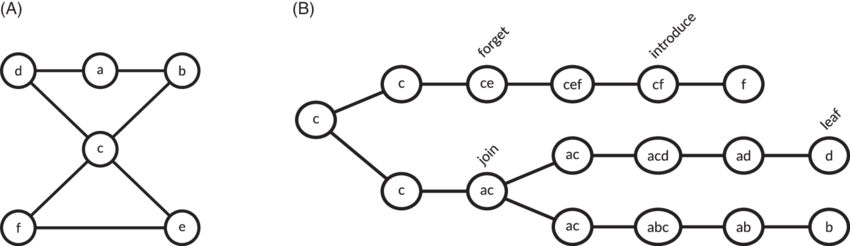
\includegraphics[width=0.95\textwidth]{./assets/nice_tree_decomposition}
	\end{center}
	\caption[Nice tree decomposition]{
		An example of a~nice tree decomposition with width three.
		On the~left, you can see the~decomposed graph,
		on the~right, a~nice tree decomposition
		with \LeafNode{}s on the~right and the~\RootNode{} on the~left.
		Figure inspired by~\cite{nice_tree_decomposition_img}.
	}%
	\label{fig:nice_tree_decomposition}
\end{figure}

An example of a nice tree decomposition with bags showed in~vertices
is shown in~\cref{fig:nice_tree_decomposition}.
%
Note that a~vertex \( v \in V(G) \) can be introduced multiple times
(in multiple branches of \( T \)),
but forgotten only once.
%
Otherwise, there must be an~\IntroduceVertexNode{} above a~\ForgetVertexNode{} in~\( T \).
But then there are multiple subgraphs in~\( T \)
such that \( v \) is in~their every bag.
This does not fulfill the~definition of a~tree decomposition.

By \( V_t, t \in T \), we~denote the~set of vertices introduced by \( t \)
and all its child nodes.
%
\begin{lemma}[\cite{book_parametrized_algorithms}]
	Any tree decomposition of width at~most \( k \) can be converted to
	a~nice tree decomposition of width at~most \( k \)
	in time \( O(k^2 \cdot \max(|V(T)|, |V(G)|)) \).
	The~nice decomposition tree has at~most \( O(k|V(G)|) \) nodes.
\end{lemma}

The~problem of finding treewidth is NP-complete~\cite{tree_width_np_complete}.
Luckily, the~problem is studied a~lot and
there exist efficient approximation algorithms~\cite{tree_width_approximation}.
We~consider nice tree decompositions as given along with a~graph
and do not consider runtime required to find it.

In~\IntroduceVertexNode{} introducing \( v \), all the~edges incident to \( v \)
to vertices in~\( X_{t'} \) are usually considered while processing \( t \).
%
For~some problems, it~is beneficial to divide this operation further.
First, a~vertex \( v \) is introduced with no edges using a~\IntroduceVertexNode{},
and later all the~edges corresponding to the~vertex are introduced using new \IntroduceEdgeNode{}s
just before one of its vertices is forgotten.

We~define an~edge bag \( Y_t \subseteq E(G), t \in T \) similarly as vertex bags \( X_t \).
%
Let~\( t' \) be a~direct ancestor of~\( t \).
For~\IntroduceVertexNode{}, we~define \( Y_t = Y_{t'} \).
For~\ForgetVertexNode{} forgetting vertex \( v \),
the following condition holds: \( Y_t = Y_{t'} \setminus \{ e \in E(G) \mid v \in e\} \).
%
\begin{definition}[\IntroduceEdgeNode{}~\cite{book_parametrized_algorithms}]
	An~\IntroduceEdgeNode{} node \( t \in T \) is a~node
	labeled with an~edge \( e = \{u, v\} \in E(G) \)
	such that \( u, v \in X_t \) and with exactly one child \( t' \)
	such that \( X_t = X_{t'} \), \( Y_t \setminus Y_{t'} = \{e\} \).
	We~say that \( e \) is \emph{introduced} by \( t \).
	Each edge can be introduced at~most once in~\( T \).
\end{definition}
%
By \( E_t, t \in T \), we~denote the~set of edges introduced by \( t \)
and all its child nodes.
By \( G_t, t \in T \), we~mean the~graph \( G_t = (V_t, E_t) \).

For~edge \( \{u, v\} \in E(G) \), we~can transform a~nice tree decomposition \( T \)
by adding \IntroduceEdgeNode{}s \( t \) above \IntroduceVertexNode{}s of \( u, v \)
and bellow \ForgetVertexNode{}s of \( u, v \in T \).
%
W.l.o.g., suppose that the~\ForgetVertexNode{}~\( t_v \) of \( v \) is
an~ancestor of the~\ForgetVertexNode{}~\( t_u \) of \( u \in T \).
Let~\( t_c \) be the~only child of \( t_u \).
%
We~add \IntroduceEdgeNode{}~\( t_e \) for~edge \( \{u, v\} \)
as a~direct child of \( t_u \) and make \( t_c \) the~direct child of \( t_e \).
%
We~can update a~nice tree decomposition by doing
a~top-down tree traversal and adding \IntroduceEdgeNode{}s for~all edges.
The~transformation requires \( O(nk) \) time (as the~number of edges is bounded by \( nk \)).
From now on, we~refer only to these transformed nice tree decompositions.

%
\begin{observation}
	\label[observation]{observ:no_edges_in_nodes}
	%
	The~edge bag of each node except for~\IntroduceEdgeNode{}s
	in a (transformed) nice tree decomposition \( t \in T \) is empty.
\end{observation}
%
This can be seen that the~edges are added right before one of the~vertices
they are incident to is forgotten. \ForgetVertexNode{} removes all the~edges
that are incident to the~forgotten vertex.

%%%%%%%%%%%%%%%%%%%%%%%%%%%%%%%%%%%%%%%%%%%%%%%%%%%%%%%%%%%%%%%%%%%%%%%%%%%%%%%%
\section{Monadic second-order logic}

Monadic second-order logic~(\MSO{}) on graphs is a~logical system based on
well-known predicate logic.
In~the~world of parameterized algorithms,
it~often comes handy --- if~we are able to represent a~problem using~\MSO{},
then there exists an~FPT algorithm parameterized by treewidth
that can solve the~problem~\cite{tree_width_mso}.

\subsection{Introduction to \( \text{MSO}_2 \)}

In~the~following paragraphs we~paraphrase and simplify formal definition
from~\cite{book_parametrized_algorithms}.
We~presume that the reader is already familiar with first-order predicate logic.
Second-order predicate logic as an~extension of first-order predicate logic,
that adds option to quantify over predicates.

\MSO{}~is realization of second-order predicate logic%
\nohznamka{
	We~need second-order logic as quantification over subsets of vertices or edges
	corresponds to quantification over predicates defining the~subsets.
	Without this requirement, we~could talk
	about the~monadic first-order logic \( \text{MSO}_1 \).
}.
Formulas can be formed from
variables, constants, predicates,
boolean operations \( \lnot, \land, \lor, \Rightarrow, \Leftrightarrow \)
and quantifiers \( \forall, \exists \).
Complex formulas are created recursively from atomic formulas
by applying schema related to each operation or quantifier.
This process is the~same as in~the~first-order predicate logic.

Formulas of \MSO{} can use four types of variables:
single vertices, single edges, subsets of vertices, and subsets of edges.
%
An~application of a~graph~\( G \) to a~formula~\( \phi \) is called \emph{evaluation}
of \( \phi \) in~\( G \).
This represents the~process of assigning values from \( G \) to variables in~\( \phi \).
%
By \( u^G \) we~denote evaluation of variable \( u \) in~graph~\( G \).
%
A~\emph{free variable} is a~variable such that it~is not quantified by any predicate.
Let~\( \Sigma \) denote all free variables of \( \phi \).
%
Let~\( \Sigma^G \) be a~sequence of evaluations for each variable in~\( \Sigma \).
Tuple \( \langle G, \Sigma^G \rangle \) is called the~\emph{structure}
in~which \( \phi \) is evaluated.
If~\( \phi \) is true in~\( \langle G, \Sigma^G \rangle \),
then \( \langle G, \Sigma^G \rangle \)
is called a~\emph{model} of \( \phi \)~\cite{book_parametrized_algorithms}.
%
To form atomic formulas in~\MSO{}, we~allow only the following base predicates:
%
\begin{itemize}
	\item For~\( u \) representing a~vertex (edge) variable
	      and \( X \) is a~vertex (edge) subset,
	      we~can write formula~\( u \in X \).
	      For~\( G \), the~formula is true if~\( u^G \in X^G \) is true.
	\item Let~\( u \) be a~vertex variable and \( e \) be an~edge variable,
	      then we~can write formula~\( \inc (u, e) \).
	      For~\( G \), the~formula is true if~\( u^G \) is an~endpoint of \( e^G \).
	\item For~any two variables \( u, v \) of the~same type, we~can write \( u = v \).
	      For~\( G \), the~formula is true if~\( u^G = v^G \).
\end{itemize}
%
We~also allow simplifications like \( \ne, \not\in \).
As obvious from types of variables, we~can quantify over vertices, edges,
subsets of vertices and subsets of edges.

It~is beneficial to define auxiliary predicates to simplify our work.
We~show examples taken from~\cite{book_parametrized_algorithms}.
First, we~show predicate \( \text{adj} \) represents if~two vertices are adjacent.
%
\begin{align*}
	\text{adj}(u, v) \coloneqq (u \ne v) \land (\exists e \in E : \inc (u, e) \land \inc (v, e))
\end{align*}
%
For~a~graph \( G = (V, E) \), we~can represent the connectivity of its induced subgraph
on vertices \( X \subseteq V \) with the~following predicate~\cite{book_parametrized_algorithms}.
%
\begin{align*}
	\text{connected}(X) \coloneqq \, &
	\forall Y \subseteq V : \Big(
	(
	\exists u \in X : u \in Y \land
	\exists v \in X : v \not\in Y
	)
	\\ &
	\Rightarrow
	(
	\exists u, v \in X : \text{adj}(u, v) \land u \in Y \land v \not\in Y
	)\Big).
\end{align*}
%
Notice that we~used our previously defined predicate as an~alias.
For~\( X = V \), the~formula would read as:
``For each separation of a~graph, there exists an~edge connecting both partitions''.

\subsection{Relation to treewidth}

In~the following, for~a~formula~\( \phi \) by \( \|\phi\| \)
we~denote the~length of the~encoding of \( \phi \) as a~string.
%
\begin{theorem}[Courcelle's theorem,~\cite{tree_width_mso,book_parametrized_algorithms}]%
	\label{theorem:courcelles_theorem}%
	Assume that \( \phi \) is a~formula of \MSO{} and
	\( G \) is an~\( n \)-vertex graph equipped
	with evaluation of all the~free variables of \( \phi \).
	Suppose, moreover, that a~tree decomposition of \( G \) of width \( k \) is provided.
	Then there exists an~algorithm that verifies whether \( \phi \)
	is satisfied in~\( G \) in~time \( f (\|\phi\|, k) \cdot n \),
	for some computable function \( f \).
\end{theorem}
%
If~we are given an~optimal tree decomposition, or we~manage to find good enough
approximation, we~know that we~can decide any formula in~\MSO{} in~a~time
polynomial in~\( n \), but we~are given no guaranties for~the~complexity~of~\( f \).

\subsection{Expressing NAC-colorings using \( \text{MSO}_2 \)}

In~this section, we~present results from our previous paper~\cite{my_paper}.
By \( V \) we~denote the~set of all vertices and
by \( E \) the~set of all edges.
We~start by defining other auxiliary predicates:
%
\begin{itemize}
	\item For~a~subset of edges \( F \), we~define predicate
	      %
	      \begin{align*}
		      \text{deg2}(F) \coloneqq \predsp
		       & \forall e \in F \predsp \forall v \in V : \inc (v, e) \Rightarrow                                                                      \\
		       & \exists e' \in F \setminus \{e\} : \Big( \inc (v, e') \land \big(\forall e'' \in F \setminus \{e, e'\}: \lnot \inc (v, e'')\big)\!\Big).
	      \end{align*}
	      %
	      The~predicate says that all vertices incident to edges in~\( F \) have degree two.
	      %
	\item For~a~subset of vertices \( U \) and a~subset of edges \( F \), we~define predicate
	      %
	      \begin{align*}
		      \text{incident}(U, F) \coloneqq \predsp
		       & \big(\forall v \in U \predsp \exists e \in F : \inc (v, e)\big)                                                       \\
		       & \land \big(\forall e \in F \predsp \exists v_1, v_2 \in U : v_1 \ne v_2 \land \inc (v_1, e) \land \inc (v_2, e)\big).
	      \end{align*}
	      %
	      The~predicate says that \( U \) are vertices of the~subgraph induced by \( F \)
	      and that \( F \) are edges of the~subgraph induced by \( U \),
	      e.g. \( (U, F) \) is an~induced subgraph of \( (V, E) \).
	      %
	\item For~a~subset of edges \( F \), we~define predicate
	      %
	      \begin{align*}
		      \text{cycle}(F) \coloneqq \predsp
		      \big( \exists X \subseteq V : \text{incident}(X, F) \land \text{connected}(X) \big)
		      \land \text{deg2}(F).
	      \end{align*}
	      %
	      The~predicate says that edges \( F \) form a~cycle.
	      %
	\item For~subsets of edges \( F_1, F_2 \), we~define predicate
	      %
	      \begin{align*}
		      \text{partition}(F_1, F_2) \coloneqq \predsp
		       & (\exists e_1, e_2 \in E : e_1 \in F_1 \land e_2 \in F_2 )    \\
		       & \land (\forall e \in E : e \in F_1 \lor e \in F_2 )          \\
		       & \land (\forall e \in E : e \not\in F_1 \lor e \not\in F_2 ).
	      \end{align*}
	      %
	      The~formula reads as: ``Both the~partitions are not empty,
	      and each edge is in~exactly one of the~partitions''.
	\item For~subsets of edges \( C, F_\red, F_\blue \), we~define predicate
	      %
	      \begin{align*}
		      \text{NACcond}(C, F_\red, F_\blue) \coloneqq \predsp
		       & C \subseteq F_\red \lor C \subseteq F_\red
		      \\
		       & \lor (\exists e_1, e_2, e_3, e_4 \in E :
		      e_1 \ne e_2 \land e_3 \ne e_4
		      \\
		       & \qquad \land e_1, e_2 \in F_\red \land e_3, e_4 \in F_\blue ).
	      \end{align*}
	      %
	      The~predicate says that the~cycles \( C \) is not an~almost cycle.
	      %
\end{itemize}
%

With the~predicates ready, we~can proceed to the~theorem.
%
\begin{theorem}[\cite{my_paper}]
	The~problem of existence of a~NAC-coloring is fixed-parameter
	tractable when parameterized by treewidth.
\end{theorem}
%
\begin{proof}
	We~can express the~NAC-coloring problem
	as a~formula~\( \phi \) in~\MSO{} as follows:
	%
	\begin{align*}
		\exists E_\red, E_\blue \subseteq E : \,
		 & \text{partition}(E_\red, E_\blue)                                                                 \\
		 & \land \big(\forall C \subseteq E : \text{cycle}(C) \land \text{NACcond}(C, E_\red, E_\blue) \big)
		.
	\end{align*}
	%
	By \Cref{theorem:courcelles_theorem},
	there exists an~FPT algorithm parameterized by treewidth
	that can resolve \( \phi \) and therefore resolve the~question whenever a~graph has a~NAC-coloring.
\end{proof}
%
The~proof shows us that there exists such an~algorithm,
but it~does not give us explicit steps to follow
(even tough they can be deduced from the~original proof of \Cref{theorem:courcelles_theorem}).
Still, the~complexity guaranties of the~algorithm are not very clear.
In~the~following section, we~define our
own FPT algorithm that solves the~NAC-coloring problem
while not relying on~\MSO{}.



\section{FPT algorithm}

In~this section, we~first introduce the~core idea of
our FPT algorithm for~NAC-coloring counting,
define a~cache function,
show and prove the~recursive formulas for~the~cache function for each node in~a~tree decomposition
and determine the~complexity of the~algorithm.
% Lastly, we~propose optimizations to the~algorithm by also empowering monochromatic classes.
We propose two approaches, one using \IntroduceEdgeNode{}s and one using \IntroduceVertexWithEdgesNode{}s.
Lastly, we~ discuss how a~certificate can be obtained
and propose additional optimizations to the~algorithm.


\subsection{The algorithm}

Our algorithm is slightly similar to Steiner tree search algorithm
as described in~\cite{book_parametrized_algorithms} as both the~problems require connectivity
among vertex partitions. Unlike in~the~Steiner tree search algorithm,
our state space is even larger and all the~state mapping operations are significantly different.

Before we~start, we~define some terms that come useful later.
When we~talk about a~component, we~mean a~connected component.
%
\begin{definition}[Connector, Neighboring components]
	For~a~graph \( G \) with a~\rbcol{} \( \gamma \)
	and two distinct components of \( G[\Ered] \), resp.\ \( G[\Eblue] \),
	with vertex sets \( U_1 \) and \( U_2 \),
	a~\emph{connector} is an~edge \( e = \{u_1, u_2\} \in E(G) \)
	such that \( u_1 \in U_1 \) and \( u_2 \in U_2 \).
	%
	The~components are \emph{neighboring} if~there exists
	a~connector for~these two components.
\end{definition}
%

First, we~want to build the~intuition for~the~upcoming operations.
Let~us have a~graph \( G \) and all NAC-colorings of the~graph \( \nac{G} \).
Let~us add an~edge \( e = \{u, v\}, e \not\in E(G) \) to form the~graph~\( G' \).
We~want to obtain~\( \nac{G'} \) based on \( \nac{G} \).
%
Let~us have \( \delta \in \nac{G} \),
we~want to extend it~to \( \delta' \) where w.l.o.g.\ \( \delta'(e) = \blue \).
Coloring \( \delta' \) is a~NAC-coloring unless an~almost cycle is formed in~\( G' \).
In~that case, one of the~following cases must be true:
%
\begin{itemize}
	\item Both vertices \( u, v \) are in~the~same component in~\( G[\Ered] \).
	      An~almost cycle is formed
	      from \( \red \) \( u \)-\( v \)-path in~the~component
	      and edge \( e \) with \( \blue \) color.
	\item Vertices \( u, v \) lay in~neighboring components in~\( G[\Eblue] \)
	      i.e.\ there is a~\( \red \) connector between the~components.
	      An~almost cycle is formed from \( \blue \) paths in~each component,
	      the~\( \red \) connector and \( \blue \) edge \( e \).
\end{itemize}
%
In~all other cases, an~almost cycle cannot be formed by adding a~\( \blue \) edge \( e \).
Note that a~vertex cannot be in~multiple components for~the~given color
as this fact would mean that the~components are not maximal.

To create \( \nac{G'} \), we~extend the~colorings
in~\( \nac{G} \cup \{ \delta_\red \} \), where \( \delta_\red \)
colors all edges in~\( G \) with \( \red \) color.
We~do the~whole checking process likewise
for~\( e \) colored \( \red \) --- all the~colors used get swapped.
Then we~keep only the~surjective colorings that did not form an~almost cycle.

We~define an~\emph{almost NAC-coloring}
as a~\rbcol{} such that there are no almost cycles formed.
The~conditions are the~same as for~NAC-coloring
except that the~surjectivity requirement is dropped.
By \( \anac{G} \), we~denote the~set of all almost NAC-colorings of \( G \).
We~use the~notion of almost NAC-coloring for~the~rest of the~section.
Later when output is read in~a~\RootNode{},
based on the~number of all almost NAC-colorings of~\( G \)
the~number of all NAC-colorings of~\( G \) is obtained.
Note that a~graph with no edges has no almost NAC-colorings.

We~use \emph{dynamic programming}, a~well-known technique for~solving problems
where the~problem can be subdivided into smaller subproblems.
Usually, some base cases are solved trivially and then a~subproblem
is solved based on the~solution of its smaller subproblems.
%
Often it~is a~case that a~smaller subproblem would be solved multiple times
as it~is a~part of multiple larger subproblems.
Its first result is therefore cached and reused,
reducing the~total running time significantly.
%
In~other cases like ours, it~is a~common approach for~traversing
some data structure like matrix or a~tree.
%
There are many popular dynamic programming algorithms
like \textsc{Edit Distance}, \textsc{Matrix Chain Multiplication} or \textsc{Longest Common Subsequence}.

In~the~following sections,
we~work with a~nice tree decomposition \( T \) of width \( k \)
of a~graph \( G \).
%
We~define a~state space \( S \) of \emph{states}
that will be used by our cache in~our dynamic programming algorithm.
We~denote all partitions of a~nonempty set \( X \) by \( \mathcal{F}(X) \),
and we~put \( \emptyset = \mathcal{F}(\emptyset) \).

%
\begin{definition}[State space]
	Let~\( t \in T \) be a~node in~the~nice tree decomposition tree and
	\( X_t \) be its bag of vertices.
	%
	A~\emph{state} is formed by a~tuple \( s = (P_\red, R_\red, P_\blue, R_\blue) \)
	where \( P_\red, P_\blue \in \mathcal{F}(X_t)\) are partitions of \( X_t \),
	and \( R_\red\), resp.\ \(R_\blue \), is a~symmetric irreflexive relation
	on parts in~\( P_\red\), resp.\ \(P_\blue \).
	%
	All such states on \( X_t \) form the~\emph{state space} \( S_t \).
\end{definition}
%
For~some \( t \in T \), a~\rbcol{} \( \gamma \) of \( G_t \)
is \emph{consistent} with a~state \( s_t = (P_\red, R_\red, P_\blue, R_\blue) \in S_t \)
if~\( \red \) and \( \blue \) components of \( \gamma \) form \( P_\red \) and \( P_\blue \)
when \( u, v \in X_t \) are in~the~same part in~\( P_\red \) or \( P_\blue \)
if~and only if~they are in~the~same \( \red \) or \( \blue \) component induced by \( \gamma \).
There are connectors between two components if~and only if
the~corresponding parts are in~relation \( R_\red \) or \( R_\blue \).
%
Note that we~define consistence for~general \rbcol{}s,
but usually we~use them with almost NAC-colorings only.
%
Two parts are \emph{neighboring} if~their corresponding components are neighboring.
When we~talk about \emph{\( \red \) half of a~state},
we~mean \( P_\red \) and \( R_\red \),
analogically for~\( \blue \).
%
Note that the~state space is somewhat large.
We~elaborate on the~size in~the~proof of~\Cref{thm:fpt_algo}.
%
\begin{observation}
	For each \rbcol{} \( \gamma \) on \( G_t \),
	there is a single state \( s \in S_t \) consistent with it.
	Multiple \rbcol{} can be consistent with a~single state.
\end{observation}
%

In~a~dynamic programming algorithms, a~cache function is gradually computed
from the~simplest subproblems to the~largest ones.
Here, we~have a~function that already has all the~values computed,
and we~show relations for~neighboring nodes in~\( T \).
There recursive relations can be then used in~an~implementation.
%
\begin{definition}[Cache function]
	For~a~nice tree decomposition \( (T, \{X_t\}) \) on a~graph \( G \),
	a~\emph{cache function} \( c: \mathcal{S} \to \N_0 \)
	where \( \mathcal{S} = \{ (t,s): t \in T \in S_t \} \)
	is the~function that maps \( (t, s) \)
	to the~number of almost NAC-colorings of \( G_t \) consistent with \( s \).
\end{definition}
%
For~the~following definitions, lemmas, proofs and theorems, let~us fix
a~nice tree decomposition \( T \) of a~graph \( G \) and width \( k \)
and a~cache function \( c \) on \( T \).
%
\begin{lemma}%
	\label[lemma]{lemma:state_space_sum}
	%
	For~\( t \in T \) and a~graph \( G_t \),
	% the following condition holds:
	\( |\anac{G_t}| =  \sum_{s \in S_t} c[t, s] \).
\end{lemma}
%
\begin{proof}
	%
	For each~\( \delta \in \anac{G_t} \),
	there is a~single state \( s \in S_t \) consistent with~\( \delta \).
	Therefore, if~we sum over all states \( s \in S_t \),
	we consider every~\( \delta \in \anac{G_t} \) and get \( |\anac{G_t}| \).
\end{proof}
%
\begin{observation}
	For~two nodes \( t_1, t_2 \in T \) such that \( G_{t_1}, G_{t_2} \)
	are isomorphic up to isolated vertices,
	then for~bags \( X_{t_1}, X_{t_2} \) and state spaces \( S_{t_t}, S_{t_2} \),
	it holds that \( \sum_{s \in S_{t_1}} c[t_1, s] = \sum_{s \in S_{t_2}} c[t_2, s] \).
\end{observation}
%
% \begin{proof}
% 	Isolated vertices are not important for~almost NAC-colorings
% 	as we~consider edges only.
% 	Therefore, as \( |\anac{G_{t_1}}| = |\anac{G_{t_2}}| \),
% 	by \Cref{lemma:state_space_sum}
% 	it holds that \( \sum_{s \in S_{t_1}} c[t_1, s] = \sum_{s \in S_{t_2}} c[t_2, s] \).
% \end{proof}
%

In~the~following lemmas, we~show recursive relations for~\( c \) that must hold
for~neighboring nodes in~\( T \).
%
In~the~following proofs,
we~often describe states that cannot be consistent with
any almost NAC-colorings and hence have zero value in~\( c \).

We~prove the correctness of our algorithms by induction.
The~base case is for~\LeafNode{}s, for~other nodes we~split the~reasoning for~cases where
there is or is not at~least one edge in~\( G_t \).
%
Following lemmas always show mapping from child node \( t' \) states \( S_{t'} \)
to parent node \( t \) states \( S_t \).
We~extend almost NAC-colorings on \( G_{t'} \) and
map which states in~\( S_{t'} \) map to which state in~\( S_t \)
or produce an~almost cycle when extended.
%
For~a~color \( a \in \{\red, \blue\} \),
we~define \( \bar{a} \) to be the~opposite color.

%%%%%%%%%%%%%%%%%%%%%%%%%%%%%%%%%%%%%%%%%%%%%%%%%%%%%%%%%%%%%%%%%%%%%%%%%%%%%%%%
% Leaf node
%%%%%%%%%%%%%%%%%%%%%%%%%%%%%%%%%%%%%%%%%%%%%%%%%%%%%%%%%%%%%%%%%%%%%%%%%%%%%%%%
\subsubsection*{\LeafNode{}}

\begin{lemma}%
	\label[lemma]{lemma:fpt_leaf_node}
	%
	Let~us have a~\LeafNode{} \( t \in T \).
	It~holds that \( c[t, s] = 0 \) for~all \( s \in S_t \).
\end{lemma}
%
\begin{proof}
	There are no edges in~\( G_t \) as there are no vertices
	neither in~\( X_t \) nor \( V_t \).
	By definition of the~cache function,
	\( c \) must hold zero for each state of a~\LeafNode{}.
\end{proof}
%
Note that for~a~\LeafNode{} \( t \in T \),
the~only state in~\( S_t \) is \( (\emptyset, \emptyset, \emptyset, \emptyset) \)
as \( X_t = \emptyset \).

%%%%%%%%%%%%%%%%%%%%%%%%%%%%%%%%%%%%%%%%%%%%%%%%%%%%%%%%%%%%%%%%%%%%%%%%%%%%%%%%
% Introduce Vertex Node
%%%%%%%%%%%%%%%%%%%%%%%%%%%%%%%%%%%%%%%%%%%%%%%%%%%%%%%%%%%%%%%%%%%%%%%%%%%%%%%%
\clearpage
\subsubsection*{\IntroduceVertexNode{}}

\begin{lemma}%
	\label[lemma]{lemma:fpt_introduce_vertex_node}
	%
	Let~an~\IntroduceVertexNode{} \( t \in T \) be
	the~only parent of \( t' \in T \).
	Let~\( v \) be the~only vertex in~\( X_t \setminus X_{t'} \).
	%
	If~there is no edge in~the~graph \( G_t \), then \( c[t, s] = 0 \) for each \( s \in S_t \).
	%
	Otherwise, the~cache function \( c \) satisfies for
	\( s=(P_\red, R_\red, P_\blue, R_\blue) \in S_t \) the~following:
	%
	\begin{align*}
		c[t, s] & =
		\begin{cases}
			0,         & \text{if } \exists a \in \{\red, \blue\} : \{v\} \not\in P_a,                    \\
			0,         & \text{if } \exists a \in \{\red, \blue\} \exists p \in P_a : (\{v\}, p) \in R_a, \\
			c[t', s'], & \text{otherwise},
		\end{cases}
	\end{align*}
	where
	\begin{align*}
		s' & \coloneqq (P_\red \setminus \{\{v\}\}, R_\red, P_\blue \setminus \{\{v\}\}, R_\blue).
	\end{align*}
\end{lemma}
%
The~state \( s' \) represents the~state where \( v \) is not present in~any part
and where the~same parts stay neighbors as in~\( s \).
%
\begin{proof}
	By definition, there are no almost NAC-colorings
	in~\( G_t \) if~\( G_t \) has no edges,
	therefore \( c[t, s] = 0 \) for each \( s \in S_t \).
	%
	Otherwise, if~a vertex \( v \) is in~a~part of \( P_\red \) or \( P_\blue \) with other vertices,
	the~cache function must be zero as \( v \) is an~isolated vertex in~\( G_t \)
	and therefore no almost NAC-coloring consistent with such state exists.
	Otherwise, there must be a~part \( \{v\} \).
	%
	Also, as \( v \) is an~isolated vertex in~\( G_t \), there cannot be a~connector
	connecting this and another component.
	Thus, for~all states where there exists
	a~part neighboring \( \{v\} \), there are no consistent almost NAC-colorings
	and therefore the~cache function must be also zero.
	%
	For~an~almost NAC-coloring \( \delta \) on \( G_{t'} \) consistent with
	a~state \( s' \in S_{t'} \),
	by adding part \( \{v\} \) to \( P_\red' \) and \( P_\blue' \)
	we get some \( s \in S_t \) that is also consistent with \( \delta \) in~\( G_t \).
	Adding and removing part \( \{v\} \) is a~bijective operation in~this context.
	Therefore, \( c[t, s] = c[t', s'] \) holds for~all states.
	%
	We~have \( anac{G_t} = anac{G_{t'}} \) since \( E(G_t) = E(G_{t'}) \).
	Each almost NAC-coloring is consistent
	with \( s \) and \( s' \) given as described.
\end{proof}
%
To summarize, values from child node are propagated to the~states
where \( v \) is added and stays isolated.

%%%%%%%%%%%%%%%%%%%%%%%%%%%%%%%%%%%%%%%%%%%%%%%%%%%%%%%%%%%%%%%%%%%%%%%%%%%%%%%%
% Forget Vertex Node
%%%%%%%%%%%%%%%%%%%%%%%%%%%%%%%%%%%%%%%%%%%%%%%%%%%%%%%%%%%%%%%%%%%%%%%%%%%%%%%%
\subsubsection*{\ForgetVertexNode{}}

\begin{lemma}%
	\label[lemma]{lemma:fpt_forget_vertex_node}
	%
	Let~a~\ForgetVertexNode{} \( t \in T \) be
	the~only parent of \( t' \in T \).
	Let~\( v \) be the~only vertex in~\( X_{t'} \setminus X_t \).
	%
	If~there are no edges in~the~graph~\( G_t \),
	then \( c[t, s] = 0 \) for each \( s \in S_t \).

	Otherwise, the~cache function for~\( s=(P_\red, R_\red, P_\blue, R_\blue) \in S_t \)
	satisfies that:
	%
	\begin{align*}
		c[t, s] & = \sum_{s' \in S'} c[t', s'],
	\end{align*}
	where for~\( a \in \{\red, \blue\} \)
	\begin{align*}
		d(p)               & \coloneqq p \setminus \{v\},                                                                                   \\
		D(P)               & \coloneqq \{d(p) \mid p \in P \} \setminus \{\emptyset\},                                                      \\
		\mathcal{P'}_a     & \coloneqq \{ P_a' \in \mathcal{F}(X_{t'}) \mid D(P_a') = P_a \},                                               \\
		\mathcal{R'}(P_a') & \coloneqq \{ R_a' \subseteq P_a' \times P_a' \mid \forall (p_1, p_2) \in R_a' :                                \\
		                   & \qquad (d(p_1), d(p_2)) \in R_a \lor d(p_1) = \emptyset \lor d(p_2) = \emptyset \},                            \\
		S'                 & \coloneqq \{(P_\red', R_\red', P_\blue', R_\blue') \mid P_a' \in \mathcal{P'}_a, R' \in \mathcal{R'}(P_a') \}.
	\end{align*}
\end{lemma}
%
Recall that \( R_\red, R_\blue \) are relations --- sets of pairs.
By \( d(p) \) we~denote deletion of the~vertex \( v \) from a~part \( p \),
and by \( D(P) \) we~denote deleting the~vertex \( v \) from all the~parts in~partition \( P \)
--- if~\( \{v\} \in P \), \( \emptyset \) is also cleared.
Set \( \mathcal{P'}_a \) denotes all the~partitions
such that removing \( v \) from them gives \( P_a \).
Mapping \( \mathcal{R'}(P_a') \) denotes all the~relations \( R_a' \)
for~\( P_a' \in \mathcal{P'}_a \) that correspond with \( R_a \) when \( v \) is removed
--- parts are updated or relations to \( \{v\} \) is removed.
States \( S' \subseteq S_{t'} \) is the~set of all states that
correspond to state \( s \) when \( v \) is removed.
%
\begin{proof}
	If~there are no edges in~\( G_t \), none are added by a~\ForgetVertexNode{}.
	Therefore, \( c[t, s] = 0 \) for~all \( s \in S_t \).
	%
	Otherwise, we~know that \( G_t = G_{t'} \).
	%
	For~\( s \in S_t \),
	let us have an~almost NAC-coloring \( \delta \) consistent with \( s \).
	We~show all states in~\( S_{t'} \) that may be consistent with \( \delta \).
	We~show how w.l.o.g.\ \( \blue \) half of \( s' \in S_{t'} \) looks
	based on \( \blue \) half of \( s \).

	Let~\( v \) be in~a~\( \blue \) component \( C \) such that
	\( C \) corresponds to no part in~\( P_\blue \).
	Then for~\( s' \) it~holds that \( \{v\} \in P_\blue' \).
	%
	Components neighboring in~\( R_\blue \)
	are also neighboring in~\( R_\blue' \), therefore \( R_\blue \subseteq R_\blue' \).
	%
	Component \( C \) may be neighboring with
	components corresponding to parts in~\( P_\blue' \).
	% It~cannot be specified with witch without deeper knowledge about \( \delta \),
	% hence we~consider all possible relations.
	To cover all possible \( \delta \),
	we consider all possible relations \( R_\blue' \).

	Now let~\( v \) in~a~component corresponding to a~part \( p \in P_\blue \).
	Then part in~\( P_\blue' \) correspond to the~same components and the~only
	change is that part \( p \) is replaced by \( p \cup \{v\} \).
	Neighboring relation is updated accordingly.

	By this we~described \( \red \) and \( \blue \) halves of states in~\( S_{t'} \)
	such that they are consistent with the~same almost NAC-colorings as \( s \).
	We~used exactly the~same operations as in~the~statement of the~lemma.

	When we~consider all states in~\( S_t \), we~cover all almost NAC-colorings on \( G_t \)
	and hence also all states in~\( S_{t'} \) must get \( s \in S_t \) to map to.

	%%%%%%%%%%%%%%%%%%%%%%%%%%%%%%%%%%%%%%%%%%
	% Old proof left for~nostalgia reasons
	%%%%%%%%%%%%%%%%%%%%%%%%%%%%%%%%%%%%%%%%%%
	% Let~us have \( \delta \in \anac{G_{t'}} \)
	% and a~consistent state \( s' \in S_{t'} \).
	% In~\( G_t \), \( \delta \) is consistent with a~state \( s \in S_t \).
	% Note that components in~\( G_t \) and \( G_{t'} \) are the~same.
	% %
	% We~now describe how w.l.o.g.\ \( \blue \) half of \( s \) looks
	% based on the~\( \blue \) half of \( s' \).
	% The~halves do not influence ech other here.
	% %
	% If~\( \{v\} \) is a~part in~\( P_\blue' \),
	% it~is no longer considered in~\( P_\blue \),
	% therefore \( P_\blue' \setminus \{\{v\}\} = P_\blue \).
	% All pairs with \( \{v\} \) are removed from \( R_\blue' \).
	% %
	% If~\( \{v\} \) is not a~part in~\( P_\blue' \),
	% \( v \) is in~another part of \( P_\blue' \).
	% In~\( P_\blue \), the~parts look the~same except they do not
	% contain~\( v \). Relation \( R_\blue' \) is updated analogically.
	% %
	% Either of these statements hold for~the~\( \blue \) half,
	% analogically for~the~\( \red \) half.
	% %
	% The~mappings we~prove are exactly \( \mathcal{P'} \) and \( \mathcal{R'} \)
	% in~the~statement of the~lemma.
	% %
	% We~showed mapping for each \( s' \in S_{t'} \) into \( S_t \).
	% %
\end{proof}
%

%%%%%%%%%%%%%%%%%%%%%%%%%%%%%%%%%%%%%%%%%%%%%%%%%%%%%%%%%%%%%%%%%%%%%%%%%%%%%%%%
% Introduce Edge Node
%%%%%%%%%%%%%%%%%%%%%%%%%%%%%%%%%%%%%%%%%%%%%%%%%%%%%%%%%%%%%%%%%%%%%%%%%%%%%%%%
\subsubsection*{\IntroduceEdgeNode{}}

When discussing \IntroduceEdgeNode{} introducing edge \( e \),
we~first describe states in~\( S_{t} \)
that cannot be consistent with any almost NAC-coloring in~\( G_t \).
If~they can, we~call them \emph{allowed}, otherwise they are \emph{not allowed}.
Similarly, we~define this notion for~halves of a~state.
%
An~edge \emph{lies} in~a~part if~both its endpoints are in~the~part.
An~edge \emph{connects} two parts if~its endpoints are each in~one~part.
%
We~state conditions for~extending almost NAC-coloring \( \delta' \)
consistent with \( s' \in S_{t'} \)
by an~edge colored by one color first,
w.l.o.g.\ let~the~introduced edge \( e \) be colored \( \blue \).
%
To avoid confusion, note that in~the~following statements we~assume
a~state \( s \in S_t \) after the~edge \( e \) is added, not a~state \( s' \in S_{t'} \).
%
We~first state conditions for~\( \blue \) half of a~state \( s \):
%
\begin{description}
	\item[Edge \( e \) lies in~a~\( \blue \) part]
	      In~this trivial case, an~almost cycle is not created in~\( \blue \) components.
	      This is \emph{\( \blue \)-allowed}.
	      %
	\item[Edge \( e \) connects two neighboring \( \blue \) parts]
	      This causes an~almost cycle to be created as
	      components corresponding to the~parts
	      are now a~single component.
	      Therefore, the~state \( s \) does not describe
	      the~actual state for~any almost NAC-coloring in~\( G_t \)
	      as there should be only a~single part, and therefore this is \emph{not allowed}.
	      %
	\item[Edge \( e \) connects two non-neighboring \( \blue \) parts]
	      This is \emph{not allowed} as both parts
	      are now using this \( \blue \) edge and should be one part.
\end{description}
%
Now we~state conditions for~\( \red \) half of a~state \( s \):
%
\begin{description}
	\item[Edge \( e \) lies in~a~\( \red \) part]
	      In~this case, an~almost cycle is trivially created
	      through the~\( \red \) component,
	      therefore, this is \emph{not allowed}.
	      %
	\item[Edge \( e \) connects two neighboring \( \red \) parts]
	      This is \emph{\( \blue \)-allowed} as \( e \) is a~connector and
	      therefore the~parts need to be neighboring.
	      %
	\item[Edge \( e \) connects two non-neighboring \( \red \) parts]
	      This state is \emph{not allowed} as both parts
	      are now neighboring as \( e \) is a~connector.
	      This is \emph{not allowed}.
\end{description}
%
The~same check is done analogically for~\( \red \)-allowed.
A~state is allowed if~both its halves are \( \red \)-allowed or
both the~halves are \( \blue \)-allowed.
Otherwise, a~state is not allowed.

\begin{lemma}%
	\label[lemma]{lemma:fpt_introduce_edge_node}
	%
	Let~us have an~\IntroduceEdgeNode{} \( t \in T \) that is
	the~only parent of \( t' \in T \).
	It~holds that \( X_t = X_{t'} \),
	let \( e = \{u, v\} \) be the~edge introduced by~\( t \), \( e \in Y_t \setminus Y_{t'} \).
	%
	If~there is only a~single edge \( e \) in~\( G_t \)
	(the just introduced edge~\( e \)) in~\( E_t \),
	for each state \( s = (P_\red, R_\red, P_\blue, R_\blue) \in S_t \),
	the~cache function satisfies that:
	\begin{align*}
		c[t, s] & =
		\begin{cases}
			1, & \text{if } \exists a \in \{\red, \blue\} :                                                 \\
			   & \{u\}, \{v\} \in P_a \land \{u, v\} \in P_{\bar{a}}                                        \\
			   & \land \, \{(\{u\}, \{v\}),(\{v\}, \{u\})\} = R_a \land R_{\bar{a}} = \emptyset             \\
			   & \land \, \forall z \in V_t \setminus \{u, v\} : \{z\} \in P_a \land \{z\} \in P_{\bar{a}}, \\
			0, & \text{otherwise}.
		\end{cases} \\
	\end{align*}
	%
	Otherwise, if~the~state \( s \) is not allowed, then \( c[t, s] = 0 \).
	%
	For~an~allowed state~\( s \),
	the~only states \( s' = (P_\red', R_\red', P_\blue', R_\blue') \in S_{t'} \),
	such that almost NAC-colorings consistent with \( s' \) are extended
	to almost NAC-colorings consistent with \( s \) by adding \( \blue \) edge \( e \),
	are the~states that fulfill these conditions for~their both halves:
	%
	\begin{description}
		\item[Edge lies in~a~\( \blue \) part of \( s \)]
		      There are two possibilities for~the~\( \blue \) half of a~state \( s' \).
		      %
		      The~first is condition that \( P_\blue = P_\blue' \)
		      and \( R_\blue = R_\blue' \) must hold.
		      %
		      The~other condition is that the~endpoints of \( e \)
		      must be in~different \( \blue \) parts \( p_1, p_2 \in P_\blue' \)
		      such that these parts are not neighboring, e.g.\ \( (p_1, p_2) \not\in R_\blue' \).
		      The~other parts are the~same as in~\( P_\blue \),
		      except for~part \( p = p_1 \cup p_2, p \in P_\blue \),
		      e.g.\ \( P_\blue' \setminus \{p_1, p_2\} = P_\blue \setminus \{p\} \).
		      \( R_\blue \) and \( R_\blue' \) must also match accordingly.
		      %
		      Either of the~conditions has to be fulfilled.

		      % First we~query the~previous cache state with
		      % the~same partition and neighbors state.
		      % Then we~also need to add states where
		      % both the~components were not neighbors as no almost cycle was created
		      % and both the~separate components
		      % are now joined into a~single component.
		      % We~denote \( \blue \) components of such state
		      % as \( P_\blue' \) and \( R_\blue' \).
		      % Note, that other relations between partitions need to match.
		      %
		\item[Edge connects two neighboring \( \red \) parts of \( s \)]
		      There are two possibilities for~the~\( \red \) half of a~state \( s' \).
		      %
		      The~first condition is that \( P_\red = P_\red' \)
		      and \( R_\red = R_\red' \) must hold.
		      %
		      Now, let~\( p_1, p_2 \in P_\red \) be the~\( \red \) parts
		      of end vertices of \( e \).
		      The~other condition is that \( P_\red = P_\red' \) and
		      \( R_\red \setminus \{(p_{1}, p_{2}), (p_{2}, p_{1})\} = R_\red' \) must hold.
		      %
		      Either of the~conditions has to be fulfilled.

		      % Result is a~sum of previous states with the~same partitioning as \( P_\red \),
		      % for~first query we~use \( R_\red \),
		      % and then we~add query of \( R'_\red = R_\red \setminus \{(c(u), c(v)), (c(v), c(u))\} \)
		      % (with the~neighbor constraint removed).
	\end{description}
	%
	There are four distinct states \( s_1', s_2', s_3', s_4' \in S_{t'} \)
	that fulfil these conditions, one for each condition combination.
	%
	We~define a~function \( c_\blue \) that represents
	the~number of all almost NAC-colorings
	consistent with state \( s \in S_t \) on \( G_t \)
	where \( e \) is colored \( \blue \).
	The~value for~\( c_\blue \) satisfies that:
	%
	\begin{align*}
		c_\blue[t, s] & = c[t', s_1'] + c[t', s_2'] + c[t', s_3'] + c[t', s_4'].
	\end{align*}
	%
	The~same holds for~\( \red \) analogously.
	Cache function satisfies that  \( c[t, s] = c_\red[t, s] + c_\blue[t, s] \).
\end{lemma}
%
\begin{proof}
	For~the~case when \( e \) is the~only edge,
	there are exactly two almost NAC-colorings on \( G_t \).
	The~states consistent with these colorings are \( s_\red \) and \( s_\blue \)
	such that if~\( u, v \) are in~the~same part in~\( P_\red \), resp.\ \( P_\blue \),
	there are parts \( \{u\}, \{v\} \) (singletons) in~\( P_\blue \), resp.\ \( P_\red \),
	as these vertices cannot be yet connected by \( \blue \), resp.\ \( \red \), edges.
	Edge \( e \) is a~connector, so there must be a~corresponding neighboring
	relation \( (\{u\}, \{v\}) \in R_\blue \), resp.\ \( R_\red \).
	Other states are not consistent with any almost NAC-colorings.
	This is exactly what we~describe in~the~lemma.

	Otherwise, only allowed states may have consistent almost NAC-colorings on \( G_t \).
	%
	For~an~almost NAC-coloring \( \delta' \) on \( G_{t'} \),
	by adding w.l.o.g.\ a~single \( \blue \) edge \( e \),
	it is either extended to an~almost NAC-coloring \( \delta \) on \( G_t \)
	or an~almost cycle is created.

	Let~\( f \) the~only edge with a~different color in~the~almost cycle.
	Let~\( f \) be colored \( \red \).
	Then there is a~\( \blue \) path connecting its endpoints using \( e \),
	as there was no such \( \blue \) path before.
	Therefore, there must be two \( \blue \) components \( p_1', p_2' \) in~\( G_{t'} \)
	connecting endpoints of \( e \) to \( f \).
	Hence, \( f \) must be a~connector connecting \( p_1' \) and \( p_2' \),
	and parts \( p_1' \) and \( p_2' \) are neighboring.
	But we~do not consider such states in~\( s_1', \dots, s_4' \).

	Let~us now consider \( f \) is colored \( \blue \).
	Then \( e = f \) and
	there must be a~\( \red \) path in~\( G_{t'} \) connecting its endpoints.
	This path must be in~a~single \( \red \) component corresponding
	to a~\( \red \) part \( p \in P_\red' \cap P_\red \).
	But we~do not consider such states in~\( s_1', \dots, s_4' \).

	Now we~show what a~state \( s \in S_t \) is
	for colorings consistent with \( s' \in \{s_1', \dots, s_4'\} \)
	when \( \blue \) edge \( e \) is added.
	%
	First we~show the~blue half.
	If~\( e \) lies in~a~\( \blue \) part,
	both its endpoints are the~same \( \blue \) component
	for \( \delta \) and the~\( \blue \) components do not change.
	If~\( e \) connects two non-neighboring \( \blue \) parts,
	then the~\( \blue \) components merge. The~same has to be reflected in
	the~consistent state in~\( S_t \).

	If~\( e \) connects two \( \red \) components based on \( \delta \) in~\( G_t \),
	they are neighboring now independently if~they were or were not neighboring before.
	The~\( \red \) components itself do not change.

	By this we~showed that all almost NAC-colorings on \( G_{t'} \) consistent with
	states \( s_1', \dots, s_4' \) are extended to almost NAC-colorings on \( G_t \)
	consistent with \( s \) where \( e \) is colored \( \blue \).
	States \( s_1', \dots, s_4' \) are the~only states in~\( S_{t'} \) mapped to~\( s \).
	We~also covered all states in~\( S_{t'} \).
	%
	When the~same is done for~\( \red \), all the~possible extensions
	of almost NAC-colorings on \( G_{t'} \) to almost NAC-colorings on \( G_t \)
	are covered.
\end{proof}

%%%%%%%%%%%%%%%%%%%%%%%%%%%%%%%%%%%%%%%%%%%%%%%%%%%%%%%%%%%%%%%%%%%%%%%%%%%%%%%%
% Join node
%%%%%%%%%%%%%%%%%%%%%%%%%%%%%%%%%%%%%%%%%%%%%%%%%%%%%%%%%%%%%%%%%%%%%%%%%%%%%%%%
\subsubsection*{\JoinNode{}}

In~the~following paragraphs,
we~first define term and prove lemmas
that come useful later in~\Cref{lemma:fpt_join_node}.
%
Let~us have a~\JoinNode{} \( t \in T \) that is
the~only parent of \( t_1', t_2' \in T \).
It~holds that \( X_t = X_{t_1}' = X_{t_2}' \),
\( G_{t_1'} \ne G_{t_2'} \)
and \( S_t = S_{t_1'} = S_{t_2'} \)
(we abbreviate them to \( S, S_1', S_2' \)).
%
For~two \rbcol{}s \( \gamma_1', \gamma_2' \)
on \( G_{t_1'} \) and \( G_{t_2'} \)
where \( E(G_{t_1'}) \cap E(G_{t_2'}) = \emptyset \),
the~\emph{merge} of \( \gamma_1' \) and \( \gamma_2' \)
is a~\rbcol{} \( \gamma : E(G_t) \to \{ \red, \blue \} \) on \( G_t \)
such that \( \forall e \in E(G_{t_1'}) : \gamma(e) = \gamma_1'(e) \) and
\( \forall e \in E(G_{t_2'}) : \gamma(e) = \gamma_2'(e) \).
%
For~a~state \( s \in S \), we~find the~set of
pairs \( (s_i', s_2') \in S_i' \times S_2' \),
whose consistent almost NAC-coloring are merged
to almost NAC-coloring consistent with \( s \).

First, we~define an~operation that shows for~two states \( s_1', s_2' \)
which state is consistent with coloring merged from \( s_1' \) and \( s_2' \).
%
\begin{definition}%
	\label[definition]{def:fpt_merging_map}
	%
	A~\emph{merging map} \( M: S_1' \times S_2' \to S \)
	maps \( s_1', s_2' \) to the~state \( s \)
	such that the~almost NAC-colorings consistent with \( s_1' \) and \( s_2' \)
	merged together are \rbcol{}s consistent with \( s \).
\end{definition}
%
It~may not be obvious that for~every coloring pair consistent with \( s_1', s_2' \)
there is a~singe state \( s \in S \) consistent with the~merged \rbcol{}.
In~the~following construction, we~show that
only the~parts of \( s_1', s_2' \) determine \( s \).
Later we~filter out \rbcol{}s that contain an~almost cycle.

Let~\( R^* \) denote the~reflexive-transitive closure of a~relation \( R \).
For each \( i \in \{1, 2\} \), let~us have states
\( s_i' = (P_{i,\red}', R_{i,\red}', P_{i,\blue}', R_{i,\blue}') \in S_i' \).
%
We~process \( \red \) and \( \blue \) halves of the~states separately.
For each \( a \in \{\red, \blue\} \),
we~take equivalence relations \( O_{i, a}' \)
whole equivalence classes are the~partitions \( P_{i, a}' \),
\( P_{i, a}' = \equivclass{X_t}{O_{i, a}'}\).
We~set
%
\begin{equation}%
	\label{eq:fpt_reflexive_transitive_closure}
	\begin{aligned}
		O_a & \coloneqq {(O_{1, a}' \cup O_{2, a}')}^*, \\
		P_a & \coloneqq \equivclass{X_t}{O_a}.
	\end{aligned}
\end{equation}
%
This operation represents merging colored components from both the~states
--- if~multiple components intersect, they become one
component and therefore one part.

We~continue with neighbor relations. We~remove pairs of parts
that were merged and update the~relations to correspond with the~new parts.
For each~\( i \in \{1, 2\} \) and for each \( a \in \{\red, \blue\} \) let
%
\begin{align*}
	R_{i,a} & \coloneqq \{(p_1, p_2) \in P_a \times P_a \mid p_{1} \ne p_{2} \, \land                                                 \\
	        & \qquad \exists p_1', p_2' \in P_{i,a}' : (p_1', p_2') \in R_{i,a}' \land p_1' \subseteq p_1 \land p_2' \subseteq p_2\},
\end{align*}
%
and let~\( R_a \coloneqq R_{1,a} \cup R_{2,a} \).

\begin{lemma}%
	\label[lemma]{lemma:fpt_merging_map}
	%
	For~a~merging map \( M \), it~holds that:
	\[ M(s_1', s_2') = (P_\red, R_\red, P_\blue, R_\blue). \]
\end{lemma}
%
\begin{proof}
	For each \( i \in \{1, 2\} \),
	let us have an~almost NAC-colorings \( \delta_i' \) consistent with
	\( s_i' \) in~\( G_{t_i'} \).
	We~merge the~two almost NAC-colorings \( \delta_1' \) and \( \delta_2' \)
	to obtain a~\rbcol{} \( \gamma \) on \( G_t \).
	This is possible as \( Y_t = \emptyset \) for~a~\JoinNode{}.
	%
	Let~us find colored components in~\( G_t \) according to \(	\gamma \).
	The~components have to be naturally the~same or larger
	than the~components in~\( G_{t_1'} \) and \( G_{t_2'} \).
	%
	If~two \( \blue \) components \( C_1', C_2' \),
	one from \( G_{t_1'} \) with \( \delta_1' \) and
	the~other from \( G_{t_2'} \) with \( \delta_2' \),
	are merged into one \( \blue \) component \( C \) in~\( G_t \),
	there must be a~\( \blue \) path connecting them.
	The~path must visit vertices \( p_1, \dots, p_l \in X_t \)
	and switch from \( \blue \) components in~\( G_{t_1'} \)
	to \( \blue \) components in~\( G_{t_2'} \) or the~other way around.
	%
	The~reflexive-transitive closure in~\Cref{eq:fpt_reflexive_transitive_closure}
	ensures that all parts corresponding to visited \( \blue \) components
	get merged into common part \( p \in P_a \).
	This part naturally corresponds to the~component \( C \) in~\( G_t \).
	%
	If~two components \( C_1, C_2 \) corresponding to
	parts \( p_1', p_2' \in P_{i,a}' \) in~\( G_{t_i'} \) are neighboring,
	all the~parts merged with them preserve the~property
	(unless \( p_1' \) gets merged with \( p_2' \) to preserve irreflexivity).
	%
	Hence, \( s = M(s_1', s_2') \) is consistent with \( \gamma \).
\end{proof}

Now we~define a~notion of filtering out
merges that do not produce almost NAC-colorings.
%
\begin{definition}%
	\label[definition]{def:fpt_bad_states}
	%
	A~pair \( (s_1', s_2') \in S_1' \times S_2'\) is \emph{bad}
	if almost NAC-colorings \( \delta_1', \delta_2' \)
	consistent with \( S_1 \) and \( S_2 \) are merged
	into \rbcol{} \( \gamma \) consistent with \( s = M(s_1', s_2') \),
	but an~almost cycle is created in~\( G_t \) considering \( \gamma \).
	%
	We~denote the~set of all bad states by \( \mathcal{B} \).
\end{definition}
%
\begin{lemma}%
	\label[lemma]{lemma:fpt_join_bad_states}
	%
	Let~\( (s_1', s_2') \in S_1' \times S_2' \),
	\( s_i' = (P_{i,\red}', R_{i,\red}', P_{i,\blue}', R_{i,\blue}') \),
	and \( s = M(s_1', s_2')
	= (P_\red, R_\red, P_\blue, R_\blue) \in S_t \).
	For each \( a \in \{\red, \blue \} \),
	\( (s_1', s_2') \in \mathcal{B} \) if~and only if
	there exists \( p \in P_{a} \)
	and \( P_{i, a}'' \subseteq P_{i, a}' \)
	such that \( \bigcup_{p' \in P_{i, a}''} p' = p \)
	and there exists \( p_1', p_2' \in P_{i, a}'' : (p_1', p_2') \in R_{i, a}' \).
\end{lemma}
%
\begin{proof}
	We~show that \( (s_1', s_2') \) is not bad only if~the~state \( s \)
	can be consistent with any almost NAC-coloring on \( G_t \)
	merged from almost NAC-colorings on \( G_{t_1'} \) and \( G_{t_2'} \)
	consistent with states \( s_1' \) and \( s_2' \).

	For~almost NAC-colorings \( \delta_1', \delta_2' \) on \( G_{t_1'}, G_{t_2'} \)
	consistent with \( s_1', s_2' \),
	we want to show how state \( s \in S \) looks and
	whether \rbcol{} \( \gamma \) created by merging \( \delta_1' \) and \( \delta_2' \)
	is an~almost NAC-coloring.
	We~show that this only depends on the~states \( s_1', s_2' \),
	not on the~structure of \( \delta_1' \) and \( \delta_2' \).

	% If~there exists an~almost cycle => the~described checks hold
	First, let~us go through cases how can an~almost cycle be created.
	%
	Suppose \( f \) is the~only edge with different color
	in an~almost cycle and let~it be w.l.o.g.\ colored \( \red \).
	Then there must exist a~\( \blue \) path connecting its endpoints.
	W.l.o.g.\ let~\( f \in E_{t_1'} \).
	%
	If~the~path spans only vertices
	in~\( V_{t_1'} \), \( \delta_1' \) is not an~almost NAC-coloring.
	%
	Therefore, \( f \) must be
	a~connector connecting two \( \blue \) components \( p_1', p_2' \in P_{1,\blue} \),
	and the~path has to also visit multiple vertices in~\( V_{t_2'} \).
	As shown in~the~proof of the~merging map \( M \), \( \blue \) components
	visited by such a path are merged together.
	%
	Such an~almost cycle therefore occurs
	if and only if~\( p_1' \) and \( p_2' \) are neighboring in~\( R_{1,\blue}' \),
	and they get merged to \( p \in P_\blue \).
	These are the~only possibilities how an~almost cycle can be created.
	%
	If~also done for~almost cycles with a~\( \blue \) edge,
	these are exactly the~bad states.
	%

	% If~the~described properties hold => there is an~almost cycle
	For~the~other direction, we~show that if~\( (s_1', s_2') \in \mathcal{B} \),
	there exists an~almost cycle
	in~\rbcol{} \( \gamma \) consistent with \( s = M(s_1', s_2') \)
	merged from almost NAC-colorings \( \delta_1' \) and \( \delta_2' \)
	consistent with \( s_1', s_2' \).
	%
	As \( (s_1', s_2') \in \mathcal{B} \),
	there exist \( p_1', p_2' \in P_{i, a}'' : (p_1', p_2') \in R_{i, a}' \),
	such that \( (p_1', p_2') \in R_{i, a}' \).
	There also exists \( p \in P_{a} \) such that \( \bigcup_{p' \in P_{i, a}''} p' = p \).
	This means that there exists a~connector \( \{u, v\} \) colored \( \bar{a} \) connecting
	components corresponding to \( p_1' \) and \( p_2' \).
	As \( p_1', p_2' \subseteq p \),
	their components on \( G_{t_i'} \) are now merged
	to a~component \( C \) on \( G_t \) colored \( a \) corresponding to \( p \).
	Then there exists a~\( u \)-\( v \)-path in~\( C \) colored \( a \).
	An~almost cycle is created from this path and the~connector \( \{u, v\} \).
\end{proof}
%

Now we~show the~recursive constraint of the~cache function \( c \) for~\JoinNode{}s.
%
\begin{lemma}%
	\label[lemma]{lemma:fpt_join_node}
	%
	Let~us have a~\JoinNode{} \( t \in T \) that is
	the~only parent of \( t_1', t_2' \in T \),
	merging map \( M \),
	and bad states \( \mathcal{B} \).

	If~both \( G_{t_1'} \) and \( G_{t_2'} \) have no edges,
	then \( c[t, s] = 0 \) for each \( s \in S \).
	If~only one of \( G_{t_1'} \) and \( G_{t_2'} \) has no edges,
	w.l.o.g.\ let~\( G_{t_1'} \) have no edges,
	then \( c[t, s] = c[t_2', s] \) for each \( s \in S \).
	%
	Otherwise, both \( G_{t_1'} \) and \(G_{t_2'} \) have some edges.
	Then for~the~cache function \( c \) it~holds that:
	%
	\begin{align*}
		c[t, s] & = \sum_{(s_1', s_2') \in \mathcal{S}(s) \setminus \mathcal{B}} c[t_1', s_1'] \cdot c[t_{2}', s_{2}']
	\end{align*}
	where
	\begin{align*}
		\mathcal{S}(s) & \coloneqq \{(s_1', s_2') \in S_{t_1'} \times S_{t_2'} \mid M(s_1', s_2') = s \}.
	\end{align*}
	%
\end{lemma}
%
% The~formula for~the~cache function comes from
% the~same idea as the~Cartesian product and
% NAC-product (\Cref{def:NACproduct}).
% The~size of such products is multiple of the~numbers of
% almost NAC-colorings on \( G_{t_1'} \) and \( G_{t_2'} \).
%
\begin{proof}
	By \Cref{def:fpt_merging_map}
	\( \mathcal{S}(s) \) is a~set of
	all pairs of states in~\( S_{t_1'} \times S_{t_2'} \)
	such that almost NAC-colorings consistent with \( s_1' \) and \( s_2' \)
	are merged to \rbcol{}s consistent with \( s \).
	As shown in~\Cref{lemma:fpt_join_bad_states},
	these \rbcol{}s are almost NAC-colorings consistent with \( s \)
	when we~do not consider bad states \( \mathcal{B} \).
	%
	For each pair of almost NAC-colorings \( \delta_1', \delta_2' \)
	consistent with \( s_1', s_2' \) such that \( (s_1', s_2') \) is not bad,
	there is one almost NAC-coloring~\( \delta \) consistent with \( s \)
	obtained by merging \( \delta_1' \) and \( \delta_2' \).
	There are \( c[t_1', s_1'] \cdot c[t_2', s_2'] \) such coloring pairs, and
	when we~sum over all such states in~\( \mathcal{S}(s) \setminus \mathcal{B} \)
	we get that \( c[t, s] \ge c[t_1', s_1'] \cdot c[t_2', s_2'] \).
	%
	For~the~opposite inequality, assume that we~have
	an~almost NAC-coloring \( \delta \) on \( G_t \) consistent with \( s \)
	that is not accounted for~by merging some \( \delta_i' \).
	But a~restriction of \( \delta \) onto \( G_{t_i'} \) produces an~almost NAC-coloring
	consistent with \( s_i' \) for each \( i \in \{1,2\} \).
	This concludes the~statement.
\end{proof}
%

\subsubsection*{\RootNode{}}

%
\begin{lemma}%
	\label[lemma]{lemma:fpt_root_node}
	Let~us have a~\RootNode{} \( r \in T \) with unique child \( t' \).
	Then \( c[r, (\emptyset,\emptyset,\emptyset,\emptyset)] = c[t', (\emptyset,\emptyset,\emptyset,\emptyset)] \).
\end{lemma}
%
\begin{proof}
	The~cache function \( c \) holds for~\( t' \) the~number of almost NAC-colorings on \( G_{t'} \).
	As \( G_{t'} = G_r \), the~number of almost NAC-colorings on \( G_r \) is the~same.
	Also, as \( X_t = \emptyset \), the~only state in~\( t \) and \( t' \) are as stated.
\end{proof}
%

\subsubsection*{All done}

%
\begin{theorem}%
	\label[theorem]{thm:fpt_algo}
	%
	There exists an~FPT algorithm
	that for~a~given nice three decomposition \( T \) of \( G \)
	can find the~number of NAC-colorings of \( G \) in~time
	\( {k}^{O(k)} \cdot 2^{O(k^2)} \cdot O(n) \), where \( n \) is the~number of vertices of \( G \)
	and \( k \) is the~width of \( T \).
\end{theorem}
%
\begin{proof}
	We~compute values of the~cache function on \( T \) in~a~bottom-up manner
	by using recursive formulas from
	\Cref{%
		lemma:fpt_leaf_node,%
		lemma:fpt_introduce_vertex_node,%
		lemma:fpt_forget_vertex_node,%
		lemma:fpt_introduce_edge_node,%
		lemma:fpt_join_node,%
		lemma:fpt_root_node%
	}.
	We~read the~output of the~\RootNode{} \( r \) as follows:
	%
	\begin{align*}
		\text{output} \coloneqq \max\{c[r, (\emptyset,\emptyset,\emptyset,\emptyset)] - 2, 0\}.
	\end{align*}
	%
	This gives us the~number of NAC-colorings of \( G \) as \( G = G_r \).
	If~the~graph has no edges, we~read \( 0 \), that is why we~use \( \max{} \) in~the~reading.
	By definition, cache function \( c \) always stores the~number of almost NAC-colorings.
	There are only two almost NAC-colorings
	that are not NAC-colorings (the monochromatic ones), and they get subtracted.
	Based on that, it~can be clearly seen that the~algorithm
	will never give you up~\cite{never_gonna_give_you_up}.

	Bell numbers are defined as
	the~number of partitions of a~set with \( n \) elements.
	They can be upper bounded by \( n^n \), which is what we~use from now on.
	Recall that \( \forall t \in T : |X_t| \le k+1 \).
	%
	First, the~size of the~state space used is upper bounded.
	For each color, there is up to \( {(k+1)}^{(k+1)} \) partitions of a~bag and
	up to \( 2^{\binom{k}{2}} \) neighboring relations.
	The~total state space size for each bag is therefore bounded by
	\[ {\Big({(k+1)}^{(k+1)} \cdot 2^{\binom{k}{2}} \Big)}^2 = {(k+1)}^{2(k+1)} \cdot 2^{2 \binom{k}{2}}. \]

	We~assume the~cache function lookups and stores have constant time complexity.
	We~go through all the~nodes and state complexity of the~operations performed in~node:
	%
	\begin{description}
		\item[\IntroduceVertexNode{}]
		      We~need to fill a~state space and copy previous values into the~cache
		      which can be done in~constant time per operation,
		      so the~time complexity corresponds to the~state space size:
		      \( {k}^{O(k)} \cdot 2^{O(k^2)} \cdot O(1) \).
		\item[\ForgetVertexNode{}]
		      Although the~operation seems complex, we~just need to traverse the~state space
		      and create a target state after \( v \) is removed.
		      This can be done in~\( O(k) \) time
		      per state as only neighboring relations where \( v \) is present
		      need to be also updated.
		      The~total complexity therefore is
		      \( {k}^{O(k)} \cdot 2^{O(k^2)} \cdot O(k) \).
		\item[\IntroduceEdgeNode{}]
		      The~state space is iterated again, and we~run few simple checks and cache key constructions
		      that can be run in~\( O(k) \) time, therefore, the~final complexity stays the~same
		      \( {k}^{O(k)} \cdot 2^{O(k^2)} \cdot O(k) \).
		\item[\JoinNode{}]
		      We~iterate through product of state spaces,
		      so the~size of the~new state space is the~power of two
		      of the~otherwise used state space size.
		      This hides into the~big \( O \) notation.
		      Checks for~almost cycles can be run in~time \( O(k^2) \).
		      Thus, the~final complexity is
		      \( {k}^{O(k)} \cdot 2^{O(k^2)} \cdot O(k^2) \).
	\end{description}
	%
	There are \( O((n+m)k) \) nodes in~\( T \) where \( m \) is bounded by \( O(kn) \).
	The~final complexity of the~algorithm is therefore
	\( {k}^{O(k)} \cdot 2^{O(k^2)} \cdot O(n) \).
\end{proof}
%

\subsection{\IntroduceVertexWithEdgesNode{}}

As we~also mentioned before, FPT algorithms parameterized by treewidth
often use \IntroduceVertexNode{} in~such a~way
that edges incident to the~introduced vertex and to
the~vertices in~the~bag are also considered.
For~this section, we~call such a behaving node an~\IntroduceVertexWithEdgesNode{}.
%
We~base our approach on the~lemmas from the~previous section.
We~outline the~proof of correctness of such operation and show
that it~is actually asymptotically slower than the~originally proposed algorithm.

We~consider a~nice tree decomposition \( T \) as defined originally
with no \IntroduceEdgeNode{}s.
The~lemmas for
\LeafNode{}, \RootNode{} and \ForgetVertexNode{} hold with no changes.
%
In~the~proof of \Cref{lemma:fpt_join_node}
regarding \JoinNode{},
we~used the~fact that \( Y_t = \emptyset \).
This is not a~necessary requirement.
%
Let~us have almost NAC-colorings \( \delta_1' \) and \( \delta_2' \)
consistent with states \( s_1' \in S_{t_1'} \) and \( s_2' \in S_{t_2'} \)
such that \( f \in Y_t \) is colored w.l.o.g.\ \( \red \) in~\( \delta_1' \)
and \( \blue \) in~\( \delta_2' \).
But then \Cref{lemma:fpt_merging_map}
still detects this pair as a~bad state
as \( f \) is a~\( \red \) connector in~a (new) \( \blue \) connected component.

Let~us describe the~idea how \IntroduceVertexWithEdgesNode{} works.
Before, when a~single edge was added,
we~checked if~there is some constraint violation
--- if~an~almost cycle was formed.
The~same is also done for~\IntroduceVertexWithEdgesNode{},
but you can think of the~process as
multiple such constrains checks at~the~same time.

Let~us have an~\IntroduceVertexWithEdgesNode{} \( t \in T \) that
is the~only parent of \( t' \in T \).
Let~\( v \) be the~only vertex in~\( X_t \setminus X_{t'} \).
Let~\( F \) be the~newly considered edges,
\( F = \{ \{ u, v \} \mid u \in X_t \} \cap E(G) \).
%
Let~us have a~set \( \Lambda \) of all almost NAC-colorings on \( F \)
(trivially found for~a~star), \( |\Lambda| = 2^{|F|} \).
Let~us have a~state space \( S_\Lambda \) on \( G_F \coloneqq G_t[F] \)
and bag \( X_F \coloneqq V(G_F) \setminus \{ v \} \).
%
\begin{observation}
	A~state in~\( S_\Lambda \) is consistent with at~most one
	almost NAC-coloring in~\( \Lambda \).
	%
	For each \( a \in \{\red, \blue\} \), each
	\( s_\lambda = (P_\red, R_\red, P_\blue, R_\blue) \in S_\Lambda \)
	and each \( \lambda \in \Lambda \) consistent with \( s_\lambda \),
	%
	if \( \lambda \) is not monochromatic,
	\( {\exists p_a \in P_a} : {|p_a| > 1
	\land \forall p_a' \in P_a \setminus \{p_a\} : |p_a'| = 1} \)
	and for each \( x \in X_F \), either \( x \in p_\red \) or \( x \in p_\blue \) holds.
	%
	If~\( \lambda \) is monochromatic, then \( {\exists p_a \in P_a} : {|p_a| = |F|} \).
\end{observation}
%
This can be seen from the~fact that \( G_F \) is a~star and \( X_F \) are its rays.
If~there are two components of the~same color,
they both must span \( v \)
and therefore they are not maximal.

Hence from now on, \( S_\Lambda \) we~only consider states corresponding to
an~almost NAC-coloring in~\( \Lambda \), hence \( |S_\Lambda| = |\Lambda| \).
%
Let~us have%
\nohznamka{
	Technically, these lemmas should be adapted for~the~fact that state space \( S_\Lambda \)
	does not come from a~node in~\( T \). This is just a~technicality
	as we~have vertex bag \( C_F \), edge bag \( F \) and graph \( G_F \)
	and only these are needed for~mentioned definitions and proofs of corresponding lemmas.
	Also, isolated vertices \( X_t \setminus X_F \) should be added to \( G_F \).
	We~skip this as this is not the~main important part of the~algorithm.
}
merging map (\Cref{def:fpt_merging_map})
\( M : S_{t'} \times S_\Lambda \to S_t \).
Also let~us have bad states (\Cref{def:fpt_bad_states})
\( \mathcal{B} \subseteq S_{t'} \times S_\Lambda \).
%
With that, we~can use a slightly adapted \Cref{lemma:fpt_join_node}
from \JoinNode{}.

% Vertices \( u, v \in X_t \) share the~same \( \blue \) component if~either:
% %
% \begin{itemize}
% 	\item They shared the~same component in~\( s' \).
% 	\item There is a~\( \blue \) path in~\( F \) with coloring \( \lambda \).
% \end{itemize}
% %
% Note that \( \blue \) components created by following this procedure
% are the same as in~\( s' \) or merged \( \blue \) components of \( s' \)
% except for~\( v \) as it~is not yet in~\( X_{t'} \).
% Such \( \blue \) components are neighboring if~either:
% %
% \begin{itemize}
% 	\item They or their predecessors in~\( s' \)
% 	      were neighbors in~\( s' \).
% 	\item There is a~path in~\( F \) with
% 	      one \( \blue \) and one \( \red \) edge
% 	      according to coloring \( \lambda \).
% 	      The~\( \red \) edge becomes a~connector.
% \end{itemize}
% %
% Now the~same is done for~\( \red \).
% We~ensure that all the~rules described in~\IntroduceEdgeNode{}
% still hold for~\( s \). If~so, \( c[t, s] \pluseq c[t', s'] \).
% This all is done for each combination in~\( S' \time \Lambda \).

In~the~original algorithm for each \( v \),
\IntroduceEdgeNode{} is used \( |F| \) times
and \( \IntroduceVertexNode{} \) once, therefore added complexity for~\( v \)
is \( {k}^{O(k)} \cdot 2^{O(k^2)} \cdot (|F| + 1) = {k}^{O(k)} \cdot 2^{O(k^2)} \cdot O(k) \).
%
For~\IntroduceVertexWithEdgesNode{},
we~used the~same technique as for~\JoinNode{}.
The~complexity is lower as \( |S_\Lambda| = 2^{|F|} \) and \( |F| = O(k) \).
The~runtime complexity added for~\( v \) is therefore
\( {k}^{O(k)} \cdot 2^{O(k^2)} \cdot 2^{O(k)} = {k}^{O(k)} \cdot 2^{O(k^2)}\).

Both approaches are asymptotically equivalent,
it~remains to be seen which yields faster runtime complexity in~practice.



\subsection{NAC-coloring certificate}

To obtain a~NAC-coloring certificate or all the~NAC-colorings of a~ graph,
one approach is to traverse \( T \) top-down
and track where there are positive additions to the~cache function.
%
The~only step where edges are introduced is \IntroduceEdgeNode{}
(or \IntroduceVertexWithEdgesNode{}).
We~check if~the~edge is w.l.o.g.\ \( \blue \) by checking if~\( c_\blue[t,s] > 0 \),
setting the~edge color to blue and color remaining edges in~\( G_{t'} \) recursively.
If~we stop at~the~first NAC-coloring, we~found a~certificate in~time bounded by
the~size of \( T \)
(if we~stored metadata about contributing states in~the~bottom-up traversal).
%
When we~continue, we~can obtain all NAC-colorings.
As there can be exponentially many of them,
listing all NAC-colorings is not parameterized by \( k \) anymore.
Note that the~whole cache has to be stored in~memory
the~whole time for~this approach.

Another approach is to store an~almost NAC-coloring on \( G_t \)
for each \( s \in S_t, t \in T \) where \( c[t, s] > 0 \)
while preferring colorings that are not monochromatic.
The~runtime performance of the~algorithm degrades,
but the~whole cache does not need to be stored in~memory the~whole time.
Only a~single certificate can be obtained with this method.


%

% It~is most probably true that monochromatic classes can be used
% to reduce the~search space.
% The~statement bellow need to be formalized better
% and more refactoring for~the~cache function is needed as
% now it~would show the~lower-bound of the~number of almost NAC-colorings
% that are a~restriction of an~NAC-coloring on \( G \).
%
% Monochromatic classes can be used to significantly reduce the~state space
% that needs to be searched as sometimes we~can say that
% \( c[t, s] = 0 \) for~some \( s \in S_t, t \in T \)
% without solving corresponding sub-problems.
% %
% We~extend the~result for~monochromatic classes as follows:
% see that this is just a~generalization of the~previous theorem
% as an~edge forms a~trivial monochromatic class.
% %
% \begin{lemma}
% 	Let~us have \( t \in T \),
% 	edges \( F \subseteq Y_t \) such that
% 	they share the~same monochromatic class and form a~connected component.
% 	Let~us have vertices \( U = \{ u \mid \exists f \in F : u \in f \} \).
% 	If~for a~state \( s = (P_\red, R_\red, P_\blue, R_\blue) \in S \)
% 	it holds that
% 	\( {\forall a \in \{\red, \blue\} }:{ \forall p_a \in P_a }:{ U \not\subset p_a} \),
% 	then it~also holds that \( c[t, s] = 0 \).
% \end{lemma}
% %
% \begin{proof}
% 	For~contradiction suppose that such state is consistent with
% 	an~almost NAC-coloring \( \delta \) on \( G_t \).
% 	The~edges \( F \) has to be either \( \red \) or \( \blue \).
% 	Let~w.l.o.g.\ edges in~\( F \) be colored \( \blue \).
% 	That means that all vertices in~\( U \) are in~the~same \( \blue \) component (and part)
% 	as the~edges are from a~monochromatic class.
% 	But the~state \( s \) states that there is a~vertex \( u \in U \)
% 	that does not share a~\( \blue \) component with the~other vertices in~\( U \).
% 	Then \( \delta \) is not consistent with state \( s \).
% 	This is a~contradiction.
% \end{proof}
% %

% Lastly, we~show how \IntroduceVertexWithEdgesNode{} can be optimized.
% Colorings of \( F \) that do no match with known monochromatic classes
% are removed from \( \Lambda \). This also decreases the~size of \( S_\Lambda \).

% We~can extend this idea further by extracting colors of edges from \( Y_{t} \)
% based on \( s_t \in S_t \).
% For~example, if~the~edge in~\( Y_{t} \) lies in~a~\( \blue \) part,
% it~must be colored blue and hence
% the~other edges from the~same monochromatic class
% must be also colored blue \( \blue \).


\subsection{Connectivity}

Along with the~cache, we~can also hold information about connectivity of
vertices in~bags.
%
\begin{definition}[Connectivity map]
	Let~\( t \in T \) be a~node in~a~nice tree decomposition tree and
	\( X_t \) be a~bag of vertices.
	A~\emph{connectivity map} \( C_t \) is a~partition of \( X_t \) such that
	for each \( u, v \in X_t \), it~holds that
	\( {\exists c_t \in C_t} : {u \in c_t \land v \in c_t} \) if~and only if
	\( u, v \) are in~the~same component in~\( G_t \).
\end{definition}
%

In~\Cref{lemma:fpt_merging_map}, we~show how to merge
two halves of two states. Let~us by \( M': S_t \to \mathcal{F}(X_t) \) denote
the~operation of merging halves of a~single state by the~same means,
obtaining a~partition of \( X_t \) and dropping
the~neighboring relation as we~do not need it
(it holds that it~is empty).
%
\begin{lemma}
	Let~us have \( s \in S_t \) with a connectivity map \( C_t \).
	If~\( M'(s) \ne C_t \), then \( c[t, s] = 0 \).
\end{lemma}
%
\begin{proof}
	For~contradiction, suppose that such a state \( s \)
	is consistent with an~almost NAC-coloring \( \delta \).
	%
	For each \( c_1, c_2 \in C_t, c_1 \ne c_2, u \in c_1, v \in c_2 \)
	there is no \( u \)--\( v \)--path in~\( G_t \).
	Then there is also no path in~the~merged parts as
	they are merged along a~path in~\Cref{lemma:fpt_merging_map}.
	%
	The~same argument with the~path non-existence
	holds also in~the~other direction.
\end{proof}
%
We~show which conditions hold for~a~connectivity map
for~different types of neighboring nodes.
%
For~an~\IntroduceVertexNode{}~\( t \) with child \( t' \), it~holds that
\( C_t = C_{t'} \cup \{\{ v \}\} \).
%
For~a~\ForgetVertexNode{}~\( t \) with child \( t' \), it~holds that
\( C_t = D(C_{t'}) \)
where \( D \) is a~map from \Cref{lemma:fpt_forget_vertex_node}
deleting occurrences of the~forgotten vertex from the~partition given.
%
For~an~\IntroduceEdgeNode{}~\( t \) with child \( t' \)
where edge \( \{u, v\} \) is introduced,
if~in~\( C_{t'} \) vertices \( u, v \) are in~the~same part, \( C_t = C_{t'} \).
Otherwise, \( u, v \) are in~parts \( p_1', p_2' \), then
\( C_t \cup \{p_1', p_2'\} = C_{t'} \cup \{ p_1' \cup p_2'\} \).
%
For~a~\JoinNode{}~\( t \) with children \( t_1', t_2' \),
connectivity maps \( C_{t_1'}, C_{t_2'} \) are merged into
a~single connectivity map \( C_t \)
the~same way as when a~\JoinNode{} is processed using a merging map \( M \).
%
For~a~\LeafNode{}~\( t \),
no vertices are present yet, so for~the~connectivity map it~holds that \( C_t = \emptyset \).


\subsection{Other optimizations}

We~first introduce a~state space reduction for~edges from edge bags.
%
Note that the~following optimizations can be only used in~\IntroduceEdgeNode{}
as the~other nodes have empty edge bags by definition.
%
\begin{lemma}
	Let~us have \( t \in T \) and an~edge \( e = \{u, v\} \in Y_t \).
	If~for a~state \( s = (P_\red, R_\red, P_\blue, R_\blue) \in S_t \)
	it holds that
	\( {\forall a \in \{\red, \blue\}} : {\forall p_a \in P_a} : {u \in p_a \Rightarrow v \not\in p_a} \),
	then it~also holds that \( c[t, s] = 0 \).
\end{lemma}
%
The~lemma states that vertices \( u, v \) incident to an~edge must
be share \( \red \) or \( \blue \) part.
%
\begin{proof}
	For~contradiction, suppose that such a state is consistent
	with some almost NAC-coloring \( \delta \) on \( G_t \).
	The~edge \( e \) has to be either \( \red \) or \( \blue \).
	Let~\( e \) be colored w.l.o.g.\ \( \blue \).
	That means that both \( u, v \) are in~the~same \( \blue \) component.
	But the~state \( s \) states that \( u, v \) do not share a~\( \blue \) component.
	Then \( \delta \) is not consistent with state \( s \).
	This is a~contradiction.
\end{proof}

As discussed before, if~the~input graph has an~articulation,
we~can once again run our algorithm on each block of the~graph separately
and then multiply the~results together to get the~final result
while also considering monochromatic colorings of each block.
Note that the~same can be done for~disconnected graphs.

There is a possibility that the~algorithm can be further improved by creating
a~Monte Carlo algorithm or a~linear algebra-based algorithm that can run
in~\( O(c^k), c \in \N \) time as~\cite{book_parametrized_algorithms} suggests
for~problems with connectivity requirements.
Monte Carlo algorithms are randomized algorithms whole output may be incorrect
with some probability. As they are often faster, they are run many times
to obtain trustworthy results.
This is unfortunately far beyond the~scope of this thesis.



\chapter{Stable cuts}%
\label{chapter:stable_cuts}

\begin{chapterabstract}
	%
	We introduce relation between stable cuts and NAC-colorings.
	We summarize progress done on stable cuts existence and search.
	Lastly we briefly describe an algorithm that can find a stable cut
	for any flexible graph.
	%
\end{chapterabstract}

\section{Stable cuts}

In this chapter we focus on connected graphs only as graph cuts lose their
meaning on disconnected graphs.
%
\begin{definition}[Stable cut]
	Independent set of a graph \( G \) is set \( I \subseteq V(G) \)
	such that \( \forall u, v \in I : \{u, v\} \not\in E(G) \).
	%
	Vertex cut of a graph \( G \) is set \( C \subseteq V(G) \)
	such that \( G \setminus C \) (\( G \) with \( C \) removed)
	is a disconnected graph.
	%
	Stable cut of a graph \( G \) is a set \( S \subseteq V(G) \) such that
	\( S \) is independent set in \( G \) and also \( S \) is vertex cut in \( G \).
\end{definition}
%

Notice how stable cuts are related to NAC-colorings.
%
\begin{lemma}[\cite{legersky_original}]
	Let \( S \) be a stable cut in \( G \).
	Then \( G \) has a NAC-coloring \( \delta \).
\end{lemma}
%
\begin{proof}
	As \( S \) is a cut in \( G \), let us have corresponding partitions \( A, B \).
	We know that \( |S| < |A|, |S| < |B| \)
	as disconnected partitions are nonempty and \( G \) was connected.
	There is at least one edge incident to vertices in both \( A \) and \( B \).
	We color \( E(G[A]) \) \( \red \) and \( E(G[B]) \) \( \blue \).
	Both colors were used, so the coloring is surjective.
	We also need to show that no almost cycle was created.
	As~\cite[Lemma 2.4]{legersky_original} states, there is no almost cycle
	in a graph if and only if components \( G_\red^\delta, G_\blue^\delta \)
	are induced subgraphs of \( G \).
	That is the case as there is no edge incident to vertices in \( S \).
	It holds that \( G_\red^\delta = G[A], G_\blue^\delta = G[B] \).
	So there are no almost cycles and \( \delta \) is a NAC-coloring.
\end{proof}
%

The statement can be extended to the following simple observation.
%
\begin{corollary}[\cite{legersky_original}]
	Let \( G \) be a connected graph with \( |E(G)| \ge 2 \).
	If there is a vertex \( v \in V(G) \) such that it is
	not contained in any triangle \( C_3 \) in \( G \),
	then the graph \( G \) has a NAC-coloring.
\end{corollary}
%
\begin{proof}
	If \( v \) is in no triangle, then there is no edge interconnecting
	vertices in \( N(v) \). Therefore, \( N(v) \) is a stable cut and \( G \)
	has a NAC-coloring.
\end{proof}

You can also prove the above lemma from the fact that every cycle that
uses a vertex in \( S \) must pass
through at least one vertex in \( A \setminus S \) and \( B \setminus S \).
Such cycle has at least four edges,
at least two are \( \red \) and at least two are \( \blue \).

It is known for some classes that stable cut must exists.
\todo[inline]{Show and cite that \( 2V-4 \) are flexible}
%
\begin{theorem}[\cite{stable_cuts_2v_4}]
	Let \( G \) be a graph with \( |E(G)| \le 2|V(G)|-4 \).
	Then \( G \) contains a stable cut.
\end{theorem}
%
This result can be extended to graphs \( |E(G)| \le 2|V(G)|-3 \) with exception
for graphs from graph class \( \GSC \):
%
\begin{itemize}
	\item Triangle and prism are in \( \GSC \).
	\item If \( H, K \in \GSC \), and \( G \) is a graph
	      formed from \( H, K \) by an edge identification,
	      then also \( G \in \GSC \).
	\item If \( H, K \in \GSC \), and \( G \) is a graph
	      formed from \( H, K \) by a triangle identification,
	      then also \( G \in \GSC \).
\end{itemize}
%
%
\begin{theorem}[\cite{stable_cuts_2v_3,stable_cuts_2v_3_revisit}]
	Let \( G \) be a graph with \( |E(G)| \le 2|V(G)|-3 \). Then \( G \) contains
	a stable cut or \( G \in \GSC \).
\end{theorem}
%
Note that 2-trees (\Cref{def:2-tree})
are in \( \GSC \) by definition.
%
\begin{lemma}[\cite{stable_cuts_legersky}]
	For every \( G \in \GSC \), either \( G \) has a NAC-coloring
	or \( G \) is a 2-tree.
\end{lemma}
%
This shows that the property of having a NAC-coloring and having a stable cut
are not equivalent.

\section{Algorithms}

As proved in~\cite{stable_cuts_complexity} it is NP-complete
to decide whether a line graph with maximum degree five admits a stable cut
--- similar result as we show for NAC-coloring in a following chapter.

The papers~\cite{stable_cuts_2v_3,stable_cuts_2v_3_revisit} do not provide
an algorithm to find the stable cut (if present)
for graphs where \(|E(G)| \le 2|V(G)|-3 \),
they only provide list of claims
from whose a stable cut set can be found.
All the checks can be run in polynomial time.
Unfortunately, the list is long and beyond the scope of this thesis.

As shown in~\cite[Algorithm 1]{stable_cuts_legersky} a stable cut can be found
in a polynomial time for any flexible graph.
As mentioned before, that also includes graphs
where \( |E(G)| \le 2|V(G)| - 4 \) (not for \( |E(G)| \le 2|V(G)| - 3 \)).
Rigid component of a graph is maximal induced subgraph such that
The main idea of the algorithm works as follows:
%
\begin{itemize}
	\item Rigid components of the graphs are found.
	\item Vertices \( u, v \) from different rigid components are chosen.
	\item If neighborhood of \( u \) is a stable cut, return it.
	\item Otherwise, contract one edge of a triangle with \( u \) and start again while preserving \( u \).
\end{itemize}

Here we show pseudocode of the algorithm as described
in the original paper~\cite{stable_cuts_legersky}.
%
\begin{algorithm}[ht]
	\caption{\textsc{Stable cut of a connected flexible graph}}%
	\label{alg:stableCutFlexible}%
	\begin{algorithmic}[1]
		\Require{} a connected flexible graph $G$, vertices $u$ and $v$ not in the same rigid component of $G$
		\Ensure{} a stable cut $S$ of $G$ such that $u$ and $v$ are separated by $S$
		\If{the neighborhood of $u$ is stable}
		\State\Return{} the neighborhood of $u$
		\Else{}
		\State{} $x_1,x_2 :={}$ neighbors of $u$ such that $(u,x_1,x_2)$  is a $3$-cycle
		\For{$i\in\{1,2\}$}
		\State{} $G'_i :={}$ the graph obtained from $G$ by contracting the edge $ux_i$
		\State{} $u'_i :={}$ the vertex of $G'_i$ corresponding to the contracted edge $ux_i$
		\EndFor{}
		\If{$u'_1$ and $v$ are in different rigid components of $G'_1$}
		\State\Return{} a stable cut of $G'_1$ separating $u'_1$ and $v$
		\Else{}
		\State\Return{} a stable cut of $G'_2$ separating $u'_2$ and $v$
		\EndIf{}
		\EndIf{}
	\end{algorithmic}
\end{algorithm}
%

\Cref{alg:stableCutFlexible}
was presented as a practical result of the following theorem.
%
\begin{theorem}[\cite{stable_cuts_legersky}]
	Let \( G \) be a flexible graph and \( u, v \in V (G) \) be such that no rigid component of \( G \)
	contains both \( u \) and \( v \). Then there is a stable cut \( S \) of \( G \) that separates \( u \) and \( v \), and such that
	every rigid component of \( G \) contains at most one vertex of \( S \). Moreover, if \( G \) is 2-connected,
	then for every vertex \( v \in V(G) \), \( G \) has a stable cut avoiding \( v \).
\end{theorem}
%
Notice that \Cref{alg:stableCutFlexible}
chooses vertices \( u, v \) arbitrary as long as they do not share a rigid component.
A check ensuring that \( u \) and \( v \) are in different rigid components
has to be added on top of this seemingly random choice.
The same check holds when \( u \) is specified.

We may also want to let user choose a vertex \( u \) and find a stable cut
that avoids it or
let user choose the vertices \( u, v \) and find a stable cut
that separates them.
In this case additional checks are needed. First if only \( u \) is specified,
it may happen that it may not be avoidable if the vertex is contained
an intersection of multiple rigid components from which the graph is formed.
In such case \( u \) is an articulation vertex and the only stable cut in the graph
and the user is notified.
When both \( u, v \) are specified,
it is possible that \( u \) and \( v \) are in the same rigid components.
In that case the user is also notified.

%
\Cref{alg:stableCutFlexible}
is implemented and contributed as part of this thesis
to PyRigi~\cite{pyrigi} in pull request~\cite{pyrigi_pr_stable_cuts}.


\chapter{Algorithm for NAC-coloring search}%
\label{chapter:alg}

\begin{chapterabstract}

	As shown before it is NP-complete to decide if a graph has a NAC-coloring,
	therefore we cannot hope for an algorithm that can solve this problem in polynomial time.
	The trivial idea how to search for NAC-colorings is to
	try all the \( \red \)-\( \blue \)-edge colorings
	and check in polynomial time if a coloring given is a NAC-coloring.
	In this chapter we propose multiple optimizations to the naive approach
	and an algorithm that significantly outperforms naive approach in general case.

\end{chapterabstract}

The goal of this section is to propose algorithms to find some or all NAC-colorings of a given graph.
After recalling the solution used in \flexrilog{},
we describe an improvement of the idea of \trcon{} components in \Cref{sec:NACvalid}
and checking whether a coloring is a NAC-coloring in \Cref{sec:small_cycles}.
In \Cref{sec:combining} we sketch the idea of algorithms that
exploit combining NAC-colorings of subgraphs.
We propose heuristics for decomposing into subgraphs and merging strategies
in \Cref{sec:decomposition,sec:merging} respectively.
Although the proposed approaches are written so that all NAC-colorings are generated,
the existence of a NAC-coloring can be checked easily by stopping after finding a first one.

This chapter is based on our previous work in~\cite{my_paper},
here we describe the approaches used more in detail
and also describe other approaches that do not work as well the approaches also
shown in the paper. We evaluate performance of the algorithm in \Cref{chapter:benchmarks}.

\section{Naive approach}

A naive approach to list all NAC-colorings is to consider
all $2^{|E(G)|}$ surjective edge colorings of graph $G$ by red and blue
and check each of them in polynomial time using \Cref{lemma:is_nac_coloring}.
We call this check \IsNACColoring{}$(G, E_r, E_b)$.
To remind the reader, the idea is quite simple
--- first we create subgraphs \( G[E_\red], G[E_\blue] \).
If there is w.l.o.g.\ \( \blue \) edge \( \{u, v\} \)
and \( \{u, v\} \) share the same connected component in \( G[E_\red] \),
an almost cycle is formed from a \( \red \) \( u \)-\( v \)-path in \( G[E_\red] \)
and the \( \blue \) edge \( \{u, v\} \).

This algorithm we call \Naive{} runs in \( O(2^{|E(G)|}) \) time.
It can be sped up dramatically by considering sets of edges instead of individual edges.
For some sets of edges, we can easily see that all the edges in the set need to share
the same color in every NAC-coloring.
Now we can color the whole sets at once
and therefore reduce the time complexity to \( O(2^{c}) \)
where \( c \) is the number of described sets.
One example of such set are \trcon{} components
as defined in~\Cref{def:triangle_connected_component}.
In the following section we extend upon the idea of \trcon{} components
to reduce the search space even further.

Another simple but important observation is that the whole search space \( O(2^{c}) \)
does not need to be traversed as a NAC-coloring with colors swapped is again a NAC-coloring.
Therefore, we fix color of one set of edges and also generate NAC-colorings with colors swapped.
This cuts our runtime in half to \( O(2^{c-1}) \).
% TODO cite https://www.youtube.com/watch?v=FZ4qeJly1g0

The algorithm implemented in \flexrilog{}
considers only colorings such that \trcon{} components are monochromatic
and also ignores NAC-colorings with colors swapped.

\section{NAC-valid relations}%
\label{sec:NACvalid}

While the idea of \trcon{} components is that 3-cycles are monochromatic,
there are other cases when two edges have to have the same color,
which can further reduce the search space.
Namely, we aim to find a partition of the edge set such that each part is necessarily monochromatic
in every NAC-coloring and the number of parts is as small as possible.

\begin{definition}[NAC-valid~\cite{my_paper}]%
	\label[definition]{def:NACvalid}
	%
	An equivalence relation $\sim$ on the edge set
	of a graph $G$ is called \emph{NAC-valid}
	if for every NAC-coloring $\delta$ of $G$ it holds that
	$\forall e_1, e_2 \in E(G) :
		e_1 \sim e_2 \Rightarrow \delta (e_{1}) = \delta (e_{2})$.
	An equivalence class of a NAC-valid relation is called a \emph{monochromatic class}.
	%
\end{definition}
%
With that, we also define terms used with monochromatic classes:
%
\begin{itemize}
	\item The \emph{vertices} of a monochromatic class $M$
	      are the vertices of the subgraph $G[M]$.
	\item We call two distinct monochromatic classes \( M_1, M_2 \) \emph{neighboring},
	      if they share at least one common vertex.
	      % if the intersection of the vertices of \( M_1, M_2 \) is non-empty.
	\item The \emph{degree} of a monochromatic class \( M \) is the number of
	      monochromatic classes that are neighbors of \( M \).
\end{itemize}
%
\begin{observation}%
	\label[observation]{observ:monochromatic_classes_graph}
	Monochromatic classes behave like a graph
	where monochromatic classes are vertices and there is an edge incident to
	two monochromatic classes if they are neighboring.
\end{observation}
%

Clearly, the relation inducing \trcon{} components is NAC-valid.
The following lemma describes a way how to construct a new NAC-valid relation from another one
with possibly less monochromatic classes.

\begin{lemma}[\cite{my_paper}]%
	\label[lemma]{lemma:two_edges_and_component}
	%
	Let $\sim$ be a NAC-valid relation on $G$ and
	$\sim^\prime$ be a relation on $E(G)$ given by
	$e_{1} \sim^\prime e_{2}$ if and only if
	$e_{1} \sim e_{2}$ or there exists
	a cycle $C$ in $G$ such that $e_{1}, e_{2}$
	are edges in $C$
	and all other edges are in the same monochromatic class of $\sim$.
	Then the reflexive-transitive closure of $\sim^\prime$ is NAC-valid.
\end{lemma}
%
\begin{proof}
	%
	The condition in \Cref{def:NACvalid} is preserved under taking reflexive-transitive closure,
	so it suffices to check it only for $\sim^\prime$: if $e_1$ and $e_2$ had different colors in some NAC-coloring,
	then $C$ would be an almost cycle since $C - \{e_1,e_2\}$ is monochromatic as the relation $\sim$ is NAC-valid.
	%
\end{proof}

Note that various situations can occur:
$e_1$ or $e_2$ is in the same a monochromatic class of~$\sim$ as the rest of $C$,
or neither of them is, see \Cref{fig:two_edges_and_component}.
If each monochromatic class of $\sim$ induces a connected subgraph,
then the edges $e_1$ and $e_2$ can be supposed to be incident,
but this is not the case in general.
For instance one could introduce a NAC-valid relation such that both triangles in a 3-prism subgraph
are in the same monochromatic class, since they have the same color in all NAC-colorings of the 3-prism.

\begin{figure}[h]
	\centering
	\begin{tikzpicture}[scale=2]
		\node[vertex] (0) at (0, 0) {};
		\node[vertex] (1) at (1, 0.5) {};
		\node[vertex] (2) at (2, 0) {};
		\node[vertex] (3) at (0.5, 0.866) {};
		\node[vertex] (4) at (1.5, 0.866) {};
		\draw[redge] (0)edge(1) (1)edge(2) (0)edge(3) (1)edge(3) (1)edge(4) (2)edge(4) (3)edge(4)  ;
		\draw[edge]  (0)edge(2)  ;
	\end{tikzpicture}
	\qquad
	\begin{tikzpicture}[scale=2]
		\node[vertex] (0) at (0, 0) {};
		\node[vertex] (1) at (1, 0.5) {};
		\node[vertex] (2) at (2, 0) {};
		\node[vertex] (3) at (0.5, 0.866) {};
		\node[vertex] (4) at (1.5, 0.866) {};
		\node[vertex,label={north:$v$}] (5) at (1, 0) {};
		\draw[redge] (0)edge(1) (1)edge(2) (0)edge(3) (1)edge(3) (1)edge(4) (2)edge(4) (3)edge(4)  ;
		\draw[edge]  (0)edge(5) (2)edge(5)  ;
	\end{tikzpicture}
	\caption[Monochromatic classes advantage.]{
		An edge with adjacent vertices in a monochromatic class (left) and
		two edges with adjacent vertices in a monochromatic class (right).}%
	\label{fig:two_edges_and_component}
\end{figure}

Notice that application of \Cref{lemma:two_edges_and_component} corresponds
to merging the monochromatic classes of $e_1$ and $e_2$.
We propose to use the following NAC-valid relation:
we start with the \trcon{} components and then apply the following two steps
as long as there is some change:
%
\begin{enumerate}
	\item If there is an edge \( \{u, v\} \) such that $u$ and $v$ are vertices of
	      the same monochromatic class $M$, then merge $M$ with the monochromatic class of \( \{u, v\} \).
	\item If there are edges \( \{u, v\} \) and \( \{v, w\} \) such that $u$ and $w$ are vertices of
	      the same monochromatic class, then merge the monochromatic classes of \( \{u, v\} \) and \( \{v, w\} \).
\end{enumerate}
%
Every \trcon{} component induces a connected subgraph and also the two operations preserve
the fact that each monochromatic class induces a connected subgraph.
Hence, the resulting partition indeed forms monochromatic classes
of a NAC-valid relation by \Cref{lemma:two_edges_and_component}.
The construction can be done in polynomial time
and implemented efficiently using a Union-find data structure
as presented in the pseudocode of \Cref{alg:create_monochromatic classes}.
\todo[inline]{Consider moving \Cref{alg:create_monochromatic classes} to attachments}

\begin{algorithm}
	\caption{Create Monochromatic classes~\cite{my_paper}}%
	\label{alg:create_monochromatic classes}
	\begin{algorithmic}[1]
		\Require{} $G$

		\Ensure{} $P \gets ()$
		\Comment{} list of monochromatic classes

		\State{} $U \gets \Call{CreateUnionFind}{E(G)}$
		\Comment{} create Union-find data structure

		\ForAll{$e_{1},e_{2},e_{3} \in \Call{FindAllTriangles}{G}$}
		\State{} $U \gets \Call{Join}{U, e_{1}, e_{2}, e_{3}}$
		\EndFor{}

		\State{} $U^\prime \gets \emptyset$
		\While{$U^\prime \not= U$}
		\State{} $U^\prime \gets U$
		\Comment{} as long as changes happen

		\State{} $\lambda : V(G) \to \mathcal{P}(E(G))$
		\Comment{} monochromatic classes a vertex is member of,
		\State{}
		\Comment{} classes are represented by a single edge, defaults to $\emptyset$

		\ForAll{$uv \in E(G)$}
		\State{} $e^\prime \gets \Call{Find}{U, uv}$
		\State{} $\lambda(u) \gets \lambda(u) \cup \{e^\prime\}$
		\State{} $\lambda(v) \gets \lambda(v) \cup \{e^\prime\}$
		\EndFor{}

		\ForAll{$v \in V(G)$}
		\If{$\exists u, w \in N(v) : \lambda(u) \cap \lambda(w) \not= \emptyset$}
		\State{} $U \gets \Call{Join}{U, vu, vw}$
		\Comment{} edges are over a same component
		\EndIf{}
		\EndFor{}
		\EndWhile{}

		\State{} $P \gets \Call{Sets}{U}$

	\end{algorithmic}
\end{algorithm}

With these improvements the complexity of the naive algorithm can be often
reduced even further.

\section{Small cycles}%
\label{sec:small_cycles}

The check \IsNACColoring{} can be quite computationally expensive
considering it is called for every possible coloring,
even though it can be implemented as simple breadth-first-search.
An optimization we use is to keep a list of shorter cycles in the graph and
check if they are almost monochromatic cycles before doing the full check.
We call this improved \Naive{} algorithm \NaiveCycles{}.

The check for a single cycle can be done in linear time
in the number of monochromatic classes using bitwise arithmetic.
One cycle $C$ can reject up to $\frac{1}{|E(C)|}$ colorings,
which can be significant for small cycles.

There are often multiple and many cycles of different lengths in the graph
and for the algorithm, only a subset of them can be chosen.
If we choose too few, performance is left on the table, if too much,
we spend too much time checking the masks while saving little
by avoiding \IsNACColoring{} checks.
The number of cycles should also grow with the number of edges,
resp.\ monochromatic classes.
As stated above, smaller cycles are preferred.

Following that, we propose the following strategy.
Given a graph $G$ and $k,\ell\in \mathbb{N}$,
we adopt the idea to monochromatic classes as follows:
for every monochromatic class $M$ in $G$,
we consider all edges $\{u, v\} \in M$ such that there is a path from $u$ to $v$
in $G - M$ that uses at most $k$ monochromatic classes.
We pick up to $l$ cycles constructed from $uv$ with the corresponding
path with the least number of used monochromatic classes.
In our implementation, we take $k=4$ and $l=2$ cycles for every monochromatic class.

\section{Combining NAC-colorings of subgraphs}%
\label{sec:combining}

In our algorithm called \Subgraphs{} a graph is decomposed into subgraphs so that
the NAC-colorings of the graph can be obtained from the NAC-colorings of the subgraphs.
We introduce notation for this process of combining NAC-colorings of suitable subgraphs.

\begin{definition}[\cite{my_paper}]%
	\label[definition]{def:NACproduct}
	%
	Let $G$ be a graph with subgraphs $G_1, \dots, G_k$
	s.\ t.\ $\bigcup_{i=1}^k E(G_i) =E(G)$.
	For $1\leq i \leq k$, let $\delta^{i}_{\red}$ and
	$\delta^{i}_{\blue}$ be the monochromatic colorings of $G_i$.
	The set
	\[ \Bigl\{
		\text{surjective }\delta : E(G) \to \{\blue, \red\}
		\mid\forall i : \delta |_{E(G_i)} \in
		\nac{G_i} \cup \{\delta^{i}_{\blue}, \delta^{i}_{\red}\}
		\Bigr\}
	\]
	is called the \emph{NAC-product} of $G_1, \dots, G_k$ and denoted by $\CP(G_1, \dots, G_k)$.
	%
\end{definition}

Since the restriction of a NAC-coloring of a graph
to its subgraph is either a NAC-coloring or monochromatic,
we have $\nac{G_{1} \cup G_{2}} \subseteq \CP(G_{1}, G_{2})$.
If $G_1, \dots, G_k$ are the connected components of $G$,
then $\nac{G} = \CP(G_1,\ldots, G_k)$.
Since every cycle is contained in a single
block\footnote{A \emph{block} is a bridge or a maximal 2-connected subgraph.}
of a graph, we have that $\nac{G} = \CP(G_1,\ldots, G_k)$
for $G_1,\ldots, G_k$ being the blocks of $G$.

In order to design a faster algorithm for searching for all NAC-colorings,
we exploit the fact that for edge-disjoint graphs $G_1$ and $G_2$,
it is straightforward to construct $\CP(G_{1}, G_{2})$ once we know $\nac{G_1}$ and $\nac{G_2}$.
Then, we can get $\nac{G_{1} \cup G_{2}}$ by applying \IsNACColoring{}
to each coloring in $\CP(G_{1}, G_{2})$, see also \Cref{alg:coloring_product}.
This can significantly reduce the number of \IsNACColoring{} calls
compared to testing all red-blue-colorings of $G_{1} \cup G_{2}$.
To apply the idea on a graph $G$, we:
%
\begin{enumerate}
	\item decompose $G$ into pairwise edge-disjoint subgraphs $G_1, \ldots, G_\ell$, and
	\item compute the NAC-product $\CP(G_1, \dots, G_\ell)$ using $\nac{G_1}, \ldots, \nac{G_\ell}$
	      and filter it to get $\nac{G}$.
\end{enumerate}
%
It is also important to note that in case the merged subgraphs
have no vertices in common, we get the whole NAC-product.
No filtering is needed in such case.
%
In the following two subsections we discuss possible heuristics
for these two phases.

\begin{algorithm}
	\caption{NAC-product with filtering}%
	\label{alg:coloring_product}
	\begin{algorithmic}[1]
		\Require{} $G_1, G_2$
		\Comment{} subgraphs
		\Require{} $N_1, N_2$
		\Comment{} NAC-colorings of the subgraphs (pairs of sets of edges)

		\Ensure{} $G$
		\Comment{} merged subgraphs
		\Ensure{} $S \gets \emptyset$
		\Comment{} the NAC-colorings of $G$

		\State{} $G = (V(G_1)\cup V(G_2), E(G_1) \cup E(G_2))$

		\State{} $N_1 \gets N_1 \cup \{(E(G_1), \emptyset), (\emptyset, E(G_1))\}$
		\Comment{} the subgraphs can also be monochromatic
		\State{} $N_2 \gets N_2 \cup \{(E(G_2), \emptyset), (\emptyset, E(G_2))\}$

		\ForAll{$(E_{r_{1}}, E_{b_{1}}) \in N_1$}
		\ForAll{$(E_{r_{2}}, E_{b_{2}}) \in N_2$}
		\State{} $E_r \gets E_{r_{1}} \cup E_{r_{2}}$
		\State{} $E_b \gets E_{b_{1}} \cup E_{b_{2}}$
		\If{$\Call{IsNACColoring}{G, E_r, E_b}$}
		% \Comment{} cycles check can be also used here
		\State{} $S \gets S \cup \{(E_r, E_b)\}$
		\EndIf{}
		\EndFor{}
		\EndFor{}
	\end{algorithmic}
\end{algorithm}

\subsection{Subgraph decomposition}%
\label{sec:decomposition}

On the input, we assume the list of monochromatic classes
and an integer $k\geq 1$, and we output a list of subgraphs
such that each has at most $k$ monochromatic classes.
We describe some heuristics how to split a graph into edge disjoint subgraphs.
Here in contrast with~\cite{my_paper} we also discuss heuristics
that did not perform well.

\subsubsection{\None{}}

The strategy with the least overhead costs is to take the chunks of $k$ consecutive
monochromatic classes in the vertex input list (heuristic \None{}).
Some synthetically generated graphs are formed in such a way
that \None{} ends up performing as good as the other strategies,
this strategy usually fails when the vertex input list is shuffled.

Our general goal for the following strategies
is to maximize the number of suitable cycles in each
subgraph as cycles may form almost cycles and those help us
to reduce the search space.

\subsubsection{\Neighbors{}}

We start with a heuristic that we call \Neighbors{},
its pseudocode is in \Cref{alg:neighbors}.
The algorithm aims to mimic breadth-first-search
behavior while respecting monochromatic classes.
The goal is to find monochromatic classes that are close together.
Let $P$ be the list on monochromatic classes,
for simplicity we assume that $k$ divides $|P|$.
We will gradually divide the monochromatic classes into bags,
the output are the subgraphs induced by the monochromatic classes in each bag.

We start with $\frac{|P|}{k}$ empty bags
and all vertices of the graph labelled $open$.
First we add a random of the remaining monochromatic classes to a bag.
All the vertices of the monochromatic classes in the bag are denoted by $used$.
We take all $open$ vertices that are neighbors of the vertices in $used$ and assign
them a score. A vertex $best$ with the highest score is chosen.
The monochromatic classes corresponding to edges connecting the vertex $best$
with vertices in $used$ are then added to the bag while not exceeding its size.
The $used$ set is updated, and the algorithm continues until the bag is full.
If $open$ is empty, this iteration of the search also ends.
A new bag is chosen, and we repeat the process.

The first strategy \Neighbors{} takes as the score the number of
neighboring vertices of a vertex in the $used$ set.
The other strategy \NeighborsDegree{} is based
on the first and adds another rule ---
if the number of neighbors match, the vertex with lower degree is chosen.

\begin{algorithm}
	\caption{Heuristic \Neighbors}%
	\label{alg:neighbors}
	\begin{algorithmic}[1]

		\Require{} $G$
		\Comment{} a graph
		\Require{} $P$
		\Comment{} monochromatic classes of $G$
		\Require{} $k$, $b \gets |P|/k$
		\Comment{} target size of bags, the number of bags

		\Ensure{} $O \gets (B_1, \ldots, B_b)$
		\Comment{} bags with monochromatic classes

		\While{$P \ne \emptyset$}
		\State{} $p \gets p \in P$
		\State{} $P \gets P \setminus \{p\}$
		\Comment{} random monochromatic class

		\State{} $B \gets \underset{B_i \in O}{\arg\min} |B_i|$
		\Comment{} the most empty bag

		\State{} $used \gets \{{v \in M} \mid {M \in B } \}$
		\Comment{} vertices already used by this bag
		\State{} $open \gets  \{w \in N(u) \mid u \in used\} \setminus used $
		\Comment{} neighbors, candidates for addition

		\While{$|open| > 0 \land |B| < k$}

		\State{} $best \gets \underset{u \in open}{\arg\max}|used \cap N(u)|$
		\Comment{} vertices with the largest neighborhood

		\For{$n \in N(best) \land |B| < k$}
		\State{} $p \gets p \in P$ such that $\{best, n\} \in p$
		\State{} $P \gets P \setminus \{p\}$

		\State{} $B \gets B \cup \{p\}$

		\State{} $used \gets used \cup \{v \mid {v \in p} \}$
		\State{} $open \gets  \{w \in N(u) \mid u \in used\} \setminus used $
		\EndFor{}
		\EndWhile{}
		\EndWhile{}
	\end{algorithmic}
\end{algorithm}

\subsubsection{\CyclesMatchChunks{}}

Monochromatic classes are first ordered descending by their degree.
Then cycles are found for each monochromatic class with the same procedure
as described in \Cref{sec:small_cycles}.
The algorithm, modified version of the breadth-first-search, goes as follows:
when a stage starts, we take a component with the highest degree
that has not been marked as used yet and add it to a queue.
While the queue is non-empty, we pop the first monochromatic class,
add it the result list and mark it as used.
Then we traverse all the cycles (that we obtained before)
corresponding to the component
and add monochromatic components from the cycles to the queue.
The stage ends when the queue is empty or when \( k \) monochromatic classes
were marked as used. The whole process is repeated until
all monochromatic classes are marked as used.

\todo[inline]{Pseudocode, maybe?}

\subsubsection{\KernighanLin{}, \Cuts{}}

Kernighan-Lin algorithm~\cite{kernighan_lin} proposes a heuristic based algorithm
for partitioning a graph into two parts. It tires to minimize the edge cut between
the parts by iteratively swapping pairs of vertices from the parts.

As noted in~\Cref{observ:monochromatic_classes_graph},
monochromatic classes can be converted into a graph.
In this strategy \KernighanLin{},
Kernighan-Lin algorithm is recursively run to split the graph into parts till
parts smaller than \( k \) are reached.
We hope that smaller edge cuts will preserve more cycles among
the monochromatic classes, that often also represent cycles in the real graph.

We also tried approach \Cuts{}, where Kernighan-Lin algorithm is replaced by
more classical flow based edge cuts to split graph into parts.
With that, we loose the guarantee that the parts in recursive step
are similar in size. The resulting components should still remain similar.

Other strategies based on
sorting monochromatic components by their degree
or breadth-first-search were also tried,
but with no meaningful results.

\subsubsection{Smart split}%
\label{sec:smart_split}

We already talked how important is that the subgraphs have something in common
while we perform the filtering of the NAC-product. We also talked about the order of
subgraphs and how do merging strategies interact with them.
Goal of the following algorithm is to create and order subgraphs in a way that they usually
share property that reduces the output size while running
the filtering of the NAC-product.

The strategies for subgraph creation are generic --- they accept a graph and
the list of sizes as input and output subgraphs. We exploit this property here. We use
these strategies to divide the graph given in half by giving it appropriate
sizes (the sum of first half of subgraph sizes and the sum of the rest).
Then we split the subgraphs further until we reach desired graph sizes.
We order the created subgraphs in the tree traversal order.
By doing that we hope to ensure that most of the neighboring subgraph pairs share
some vertices and therefore more cycles appear in the merged subgraph.

Also note that \Cref{alg:smart_split} has compatible interface with
all the subgraph creation strategies and therefore can be easily added.

\begin{algorithm}
	\caption{Smart Split}%
	\label{alg:smart_split}
	\begin{algorithmic}[1]
		\Require{} $G$
		\Comment{} Subgraph to work on
		\Require{} $P$
		\Comment{} Monochromatic classes of the subgraph $G$
		\Require{} $S$, $s \gets |S|$
		\Comment{} List of the sizes of subgraphs and their number

		\Ensure{} $O \gets ()$
		\Comment{} List of ordered vertices

		\If{$s \le 2$}
		\State{} $O \gets \Call{MergeStrategy}{G, P, S}$
		\State{}
		\Return{}
		\EndIf{}

		\State{} $S_1, S_2 \gets S[:\lfloor\frac{s}{2}\rfloor], S[\lfloor\frac{s}{2}\rfloor:]$
		\State{} $P \gets \Call{SubgraphStrategy}{G, P, (\sum S_{1}, \sum S_{2})}$

		\State{} $P_1 \gets P[:(\sum S_1)]$
		\State{} $P_2 \gets P[(\sum S_1):]$
		\State{} $G_1 \gets \Call{InducedSubgraphOnEdges}{G, \bigcup P_1}$
		\State{} $G_2 \gets \Call{InducedSubgraphOnEdges}{G, \bigcup P_2}$

		\State{} $O_1 \gets \Call{SmartSplit}{G_1, P_1, S_1}$
		\State{} $O_2 \gets \Call{SmartSplit}{G_2, P_2, S_2}$
		\State{} $O \gets O_{1}.O_{2}$
	\end{algorithmic}
\end{algorithm}


\subsection{Subgraph merging}%
\label{sec:merging}

After constructing the list of edge-disjoint subgraphs,
we compute all the NAC-colorings for each of them using
the naive algorithm with monochromatic classes
and improved check on cycles.
Then the results need to be merged to obtain the NAC-colorings of the original graph
using the NAC-product.

Since checking every coloring in the NAC-product is a costly operation,
we try to minimize the work that has to be done.
The complexity of the task grows with the size of
the merged subgraphs (as \IsNACColoring{} depends on the size of the graph checked)
and also with the number of NAC-colorings found in each subgraph
(which can grow exponentially).

We describe multiple merging strategies.
As before, we extend on the list we presented in~\cite{my_paper}.
The first approach \MergeLinear{} is
to take the sequence of subgraphs and merge them one by one.
We merge the first and the second subgraph, then we merge this result with the
third one and so on. We have tried also tree-like approach, i.e., to merge consecutive pairs
and then recursively again, but the performance was worse.

Another approach called \SharedVertices{} always merges the two subgraphs that
have the most vertices in common with the goal
to create as many new cycles as possible.

Next approach called \Log{} tries to merge subgraphs in a tree like manner.
Consider we have an order list of subgraphs,
for simplicity let its size be \( 2^c \) for some \( c \in \N \).
Now, the list is split into pairs of subgraphs and NAC-colorings
of the subgraphs in pairs are merged. With that, a new list is created.
The continues until we have the original graph and all its NAC-colorings.
Note, that the approach makes little sense if~\Cref{alg:smart_split}
is not also enabled.

We consider the number of monochromatic components
that induces a given subgraph as its size.
One heuristic is that runtime can be reduced
when first small subgraphs are merged with large subgraphs
rather than large graphs with large subgraphs, as merging large graphs is expensive.
This is what \MinMax{} strategy does.
First smallest subgraph is merged with the largest one,
then second smallest with the second largest and so on.
A new list is created, and the same procedure is run on repeatedly.

Following strategy is called \PromisingCycles{}.
The strategy tries to guess which subgraphs
have the most potential almost cycles when joined.
For each pair of subgraphs we find cycles in joined subgraph using
the same routine as in \Cref{sec:small_cycles}.
A joined graph with the maximal number of cycles is chosen,
otherwise we score as follows:
%
\begin{itemize}
	\item If subgraphs share a vertex, the score grows.
	\item Smaller joined graphs get higher priority.
	\item Subgraphs with more common vertices get higher priority.
\end{itemize}
%

All the previous merging strategies did not employ the number of NAC-colorings
of individual subgraphs in merging decisions.
That is on purpose as we do not know the number of NAC-colorings in advance.
With that, if only a single NAC-coloring is needed,
in our implementation we can use lazy iterators that
find a NAC-coloring of a subgraph and wait till another coloring is requested.
If all the NAC-colorings are desired or if we expect the graph to have no NAC-coloring,
all NAC-colorings of subgraphs need to be found anyway.
In such cases we can employ heuristics that take advantage of such additional knowledge.

Our preferred strategy of this kind is called \Score{}
In each iteration a score is computed for each pair of subgraphs in the current list.
For subgraphs \( G_1, G_2 \) the score is computed by formula
\( \nnac{G_1} \cdot \nnac{G_2} \cdot \text{sizeof}(G_1 \cup G_2) \).
The score approximates the amount of work needed,
therefore the pair with the lowest score is chosen.

We also tried approaches based on dynamic programming and recursive optimization.
Unfortunately, these approached do not scale well to larger instances.

\section{Polynomial optimizations}%
\label{sec:polynomial_optimizations}
\todo[inline]{Write the section}
% stable cut observation
% to many edges
% to few edges -> stable cut
% minimally rigid if not certificate is needed

\chapter{Implementation \& Benchmarks}%
\label{chapter:benchmarks}

\begin{chapterabstract}

	In this chapter we first describe the structure of the project
	and discuss some of the design choices.
	After that, we evaluate performance of the algorithms
	proposed in \Cref{chapter:alg}.
	First, we compare the approaches with previous approaches,
	and then we compare heuristics with each other
	for different use-cases.
	We show reduction both in runtime and in the number
	of \IsNACColoring{} checks performed.

\end{chapterabstract}

\section{Implementation}

\todo[inline]{Popsat, jak/kde je kód přiložen}

In this section we first describe the structure of the project containing
the code of the algorithm.
Next, we mention libraries, relation to PyRigi and
some worth mentioning implementation details.

The code is written in Python, minimal supported version is Python 3.12.
To set up the project, create a virtual environment and install packages
from \texttt{requirements.txt}. On NixOS, you can use \texttt{shell.nix}.
See \texttt{README.md} for additional instructions.
We go through the main folders and files of the project.

In \texttt{graphs\_store} we store datasets used for benchmarking.
Graphs are either obtained from~\cite{extremal_graphs},
generated using Nauty~\cite{nauty} with a plugin~\cite{nauty_plugin}
or generated using NetworkX~\cite{networkx} and checks from PyRigi~\cite{pyrigi}.
Graph are usually stored in Graph6 format.
Code for reading graphs from the store can be found in \texttt{benchmarks/dataset.py},
code for generating some graph classes can be found in  \texttt{benchmarks/generators.py},
In the \texttt{benchmark} directory, there are all result of the benchmarks that we run
during the project development. The most relevant for a reader is the CSV file
stored in \texttt{precomputed} directory containing individual benchmark results.
The base directory contains tooling for running, visualizing and exporting benchmarks.
File \texttt{NAC\_playground.ipynb} in the root directory presents a simple case
to visualize how the Python API can be used.
File \texttt{NAC\_presentation.ipynb} shows how the basic benchmarks can be run.

The code of the algorithm described in~\Cref{sec:stable_cuts_implementation}
with additional helper functions is implemented in directory \texttt{stablecut}.
Note that some changes were done when the code was merged into PyRigi.
The code of the algorithm described in~\Cref{chapter:alg}
is stored in directory \texttt{nac}.
Directory \texttt{nac/util} stores helper functions and classes
like an implementation of the \textsc{UnionFind} data structure.
File \texttt{check.py} implements \IsNACColoring{} check.
File \texttt{monochromatic\_classes.py} is used to find \trcon{} components
and monochromatic classes in a graph. With this, we can compare performance
between using monochromatic classes, \trcon{} components or just edges.
File \texttt{cycle\_detection.py} holds algorithms for finding cycles
used in \Cref{sec:small_cycles}
and related heuristics as described in \Cref{chapter:alg}.
In \Cref{sec:polynomial_optimizations}
we presented checks that can sometimes find
a NAC-coloring or determine that there is none in polynomial time.
These checks are implemented in \texttt{existence.py} and
used mostly from \texttt{single.py} that is the entry-point for finding a single NAC-coloring of a graph.
General NAC-coloring searching is implemented in \texttt{search.py}
along with parameter processing, graph vertices relabeling,
optimizations like search for articulation vertices are performed.
After that, the correct algorithm (\Naive{}, \NaiveCycles{} or \Subgraphs{})
is chosen and called.
These algorithms are implemented in \texttt{algorithms.py} alongside many helper functions.
Heuristics for \Subgraphs{} algorithm are stored in \texttt{strategies.py}.
Tests of the whole code are stored in directory \texttt{test}.

Common function parameters are:
\textsc{graph} repressing the (sub)graph where NAC-colorings should be found,
\textsc{comp\_graph} where vertices are some integer IDs of monochromatic classes
and edges exists if the classes are neighboring.
An ID of a monochromatic class also serves as index into \textsc{component\_to\_edges}
that maps an ID of a monochromatic class to its edges.
NAC-colorings are represented as bit-masks where bit's offset correspond to a component ID.

As \IsNACColoring{} is a core component of all our algorithms, we optimize it as much as we could.
In the implementation of \IsNACColoring{}, subgraphs from \( \red \) and \( \blue \) edges are created.
To create such subgraphs in code, edges can be added to an empty graph
using NetworkX's function \textsc{add\_edges\_from}.
This is rather slow as creating new vertices in the empty graph causes noticeable overhead.
Therefore, we create a graph with no edges and the same vertices as the original graph,
cache it and reuse it for the checks. First edges are added, the check is run, and the edges are cleared.
By doing this, the performance of \IsNACColoring{} is increased by roughly forty percent.
Another way how the performance could be increased is by reserving space in lists
when the final size is known. This is unfortunately not possible in Python.

The code uses \textsc{Graph} class and related algorithms from NetworkX~\cite{networkx}
as the base of all operations. We use some utility functions from PyRigi~\cite{pyrigi}
related to rigidity tests and rigidity components search.
Otherwise, the code is not dependent on PyRigi.
Pytest is used for testing.

\section{Benchmarks}

In this section we first set meaningful targets for our benchmarks,
then we compare the performance of our algorithm with the previous implementations
and show running time and internal search optimizations for various graph classes.

The main question regarding NAC-coloring search is whether a graph has a NAC-coloring.
We usually ask the algorithm to not only answer yes, but to also provide a certificate.
For flexible graphs, it is usually algorithmically quite simple to find a NAC-coloring,
so this question is more interesting for rigid graphs.
For flexible graphs, it is more interesting to ask for the number of NAC-colorings
of a graph.
Note, that for larger flexible graphs with around thirty vertices
the number of NAC-colorings is huge as it often grows exponentially.
This slows our algorithm down as just materializing exponential
number of NAC-colorings takes exponential time.
For such cases, the FPT algorithm described in \Cref{chapter:fpt}
is a better fit as it does not materialize all the NAC-coloring on subgraphs.

The benchmarks comparing our algorithm with the previous implementations
were run on Linux on a laptop with Intel i7 of the 11th generation
with CPython 3.12 and SageMath 10.4.
The remaining benchmarks were run a laptop with Intel i5 of the 6th generation
using CPython 3.12.
On modern hardware, the times can be easily cut in half.

\subsection{Improvement over previous solutions}

\Cref{tab:all_min_rigid}
shows the time required for finding all the NAC-colorings
of all minimally rigid graphs with given size (generated using Nauty~\cite{nauty}
with a corresponding plugin~\cite{nauty_plugin}).
We show results of the implementation in \flexrilog{}~\cite{flexrilog} run in SageMath
and compare them to our implementation of the same \Naive{} algorithm
using $\triangle$-connected components
and monochromatic classes as described in \Cref{sec:NACvalid}.
Next column shows \NaiveCycles{} from \Cref{sec:small_cycles}
using monochromatic classes.
The last column is for the \NeighborsDegree{} (each initial subgraph has $k=4$ monochromatic classes)
with \MergeLinear{} merging strategy.
For twelve vertices, \Neighbors{} algorithm took around four hours for over 800k minimally rigid graphs.
In every case, our algorithms are significantly faster than implementation in \flexrilog{}~\cite{flexrilog}.
Notice also huge advantage gained by using monochromatic classes instead of \trcon{} components,
that are also used by \flexrilog{}.
%
\begin{table}[ht]
	\caption[Running times on graphs.]{
		The time (in seconds) needed to find all NAC-colorings for all graphs with a given size. Run by us.
		\textsc{FRLG} stands for \flexrilog{}, \textsc{ND} for \NeighborsDegree{}.}%
	\label{tab:all_min_rigid}
	\vspace{0.3cm}
	\centering
	\begin{tabular}{ccccccc}
		\hline
		\,$|V(G)|$\, & \,\#graphs\, & \,FRLG\, & \,$\triangle$-comps.\, & \,monochr.\, & \,cycles\, & \,\textsc{ND}\, \\
		\hline
		% 5        & 3           & 0.007 s      & 0.002 s            & 0.001 s       & 0.001 s & 0.002 s          \\
		% 6        & 13          & 0.063 s      & 0.030 s            & 0.010 s       & 0.005 s & 0.007 s          \\
		% 7        & 70          & 0.57 s       & 0.052 s            & 0.047 s       & 0.029 s & 0.041 s          \\
		8            & 608          & 14       & 1.09                   & 0.97         & 0.36       & 0.49            \\
		9            & 7\,222       & 509      & 34                     & 29           & 5.8        & 8.6             \\
		10           & 110\,132     & 27k      & 1\,725                 & 1\,446       & 151        & 213             \\
		11           & 2\,039\,273  & -        & -                      & -            & 5\,440     & 6\,650          \\
		\hline
	\end{tabular}
\end{table}

\Cref{fig:graph_time_minimally_rigid}
shows timings to compute all NAC-colorings of minimally rigid graphs
depending on the strategy used.
We did not list all NAC-coloring for minimally rigid graphs with more than twelve vertices
as there is too many such graphs.

The following dataset has been randomly generated
using NetworkX~\cite{networkx} and PyRigi~\cite{pyrigi}.
%
You can see that for graphs up to around fourteen vertices the \NaiveCycles{} algorithm
is still faster than \Subgraphs{}.
For graphs with more than eighteen vertices,
the growing advantage of \Subgraphs{} is already significant.

\begin{figure}[ht]
	\centering
	\scalebox{0.5}{%% Creator: Matplotlib, PGF backend
%%
%% To include the figure in your LaTeX document, write
%%   \input{<filename>.pgf}
%%
%% Make sure the required packages are loaded in your preamble
%%   \usepackage{pgf}
%%
%% Also ensure that all the required font packages are loaded; for instance,
%% the lmodern package is sometimes necessary when using math font.
%%   \usepackage{lmodern}
%%
%% Figures using additional raster images can only be included by \input if
%% they are in the same directory as the main LaTeX file. For loading figures
%% from other directories you can use the `import` package
%%   \usepackage{import}
%%
%% and then include the figures with
%%   \import{<path to file>}{<filename>.pgf}
%%
%% Matplotlib used the following preamble
%%   \def\mathdefault#1{#1}
%%   \everymath=\expandafter{\the\everymath\displaystyle}
%%   \IfFileExists{scrextend.sty}{
%%     \usepackage[fontsize=10.000000pt]{scrextend}
%%   }{
%%     \renewcommand{\normalsize}{\fontsize{10.000000}{12.000000}\selectfont}
%%     \normalsize
%%   }
%%   
%%   \ifdefined\pdftexversion\else  % non-pdftex case.
%%     \usepackage{fontspec}
%%     \setmainfont{DejaVuSans.ttf}[Path=\detokenize{/home/petr/Projects/PyRigi/.venv/lib/python3.12/site-packages/matplotlib/mpl-data/fonts/ttf/}]
%%     \setsansfont{DejaVuSans.ttf}[Path=\detokenize{/home/petr/Projects/PyRigi/.venv/lib/python3.12/site-packages/matplotlib/mpl-data/fonts/ttf/}]
%%     \setmonofont{DejaVuSansMono.ttf}[Path=\detokenize{/home/petr/Projects/PyRigi/.venv/lib/python3.12/site-packages/matplotlib/mpl-data/fonts/ttf/}]
%%   \fi
%%   \makeatletter\@ifpackageloaded{underscore}{}{\usepackage[strings]{underscore}}\makeatother
%%
\begingroup%
\makeatletter%
\begin{pgfpicture}%
\pgfpathrectangle{\pgfpointorigin}{\pgfqpoint{8.384376in}{2.841849in}}%
\pgfusepath{use as bounding box, clip}%
\begin{pgfscope}%
\pgfsetbuttcap%
\pgfsetmiterjoin%
\definecolor{currentfill}{rgb}{1.000000,1.000000,1.000000}%
\pgfsetfillcolor{currentfill}%
\pgfsetlinewidth{0.000000pt}%
\definecolor{currentstroke}{rgb}{1.000000,1.000000,1.000000}%
\pgfsetstrokecolor{currentstroke}%
\pgfsetdash{}{0pt}%
\pgfpathmoveto{\pgfqpoint{0.000000in}{0.000000in}}%
\pgfpathlineto{\pgfqpoint{8.384376in}{0.000000in}}%
\pgfpathlineto{\pgfqpoint{8.384376in}{2.841849in}}%
\pgfpathlineto{\pgfqpoint{0.000000in}{2.841849in}}%
\pgfpathlineto{\pgfqpoint{0.000000in}{0.000000in}}%
\pgfpathclose%
\pgfusepath{fill}%
\end{pgfscope}%
\begin{pgfscope}%
\pgfsetbuttcap%
\pgfsetmiterjoin%
\definecolor{currentfill}{rgb}{1.000000,1.000000,1.000000}%
\pgfsetfillcolor{currentfill}%
\pgfsetlinewidth{0.000000pt}%
\definecolor{currentstroke}{rgb}{0.000000,0.000000,0.000000}%
\pgfsetstrokecolor{currentstroke}%
\pgfsetstrokeopacity{0.000000}%
\pgfsetdash{}{0pt}%
\pgfpathmoveto{\pgfqpoint{0.588387in}{0.521603in}}%
\pgfpathlineto{\pgfqpoint{5.988063in}{0.521603in}}%
\pgfpathlineto{\pgfqpoint{5.988063in}{2.531888in}}%
\pgfpathlineto{\pgfqpoint{0.588387in}{2.531888in}}%
\pgfpathlineto{\pgfqpoint{0.588387in}{0.521603in}}%
\pgfpathclose%
\pgfusepath{fill}%
\end{pgfscope}%
\begin{pgfscope}%
\pgfsetbuttcap%
\pgfsetroundjoin%
\definecolor{currentfill}{rgb}{0.000000,0.000000,0.000000}%
\pgfsetfillcolor{currentfill}%
\pgfsetlinewidth{0.803000pt}%
\definecolor{currentstroke}{rgb}{0.000000,0.000000,0.000000}%
\pgfsetstrokecolor{currentstroke}%
\pgfsetdash{}{0pt}%
\pgfsys@defobject{currentmarker}{\pgfqpoint{0.000000in}{-0.048611in}}{\pgfqpoint{0.000000in}{0.000000in}}{%
\pgfpathmoveto{\pgfqpoint{0.000000in}{0.000000in}}%
\pgfpathlineto{\pgfqpoint{0.000000in}{-0.048611in}}%
\pgfusepath{stroke,fill}%
}%
\begin{pgfscope}%
\pgfsys@transformshift{1.015634in}{0.521603in}%
\pgfsys@useobject{currentmarker}{}%
\end{pgfscope}%
\end{pgfscope}%
\begin{pgfscope}%
\definecolor{textcolor}{rgb}{0.000000,0.000000,0.000000}%
\pgfsetstrokecolor{textcolor}%
\pgfsetfillcolor{textcolor}%
\pgftext[x=1.015634in,y=0.424381in,,top]{\color{textcolor}{\rmfamily\fontsize{10.000000}{12.000000}\selectfont\catcode`\^=\active\def^{\ifmmode\sp\else\^{}\fi}\catcode`\%=\active\def%{\%}$\mathdefault{3}$}}%
\end{pgfscope}%
\begin{pgfscope}%
\pgfsetbuttcap%
\pgfsetroundjoin%
\definecolor{currentfill}{rgb}{0.000000,0.000000,0.000000}%
\pgfsetfillcolor{currentfill}%
\pgfsetlinewidth{0.803000pt}%
\definecolor{currentstroke}{rgb}{0.000000,0.000000,0.000000}%
\pgfsetstrokecolor{currentstroke}%
\pgfsetdash{}{0pt}%
\pgfsys@defobject{currentmarker}{\pgfqpoint{0.000000in}{-0.048611in}}{\pgfqpoint{0.000000in}{0.000000in}}{%
\pgfpathmoveto{\pgfqpoint{0.000000in}{0.000000in}}%
\pgfpathlineto{\pgfqpoint{0.000000in}{-0.048611in}}%
\pgfusepath{stroke,fill}%
}%
\begin{pgfscope}%
\pgfsys@transformshift{1.561056in}{0.521603in}%
\pgfsys@useobject{currentmarker}{}%
\end{pgfscope}%
\end{pgfscope}%
\begin{pgfscope}%
\definecolor{textcolor}{rgb}{0.000000,0.000000,0.000000}%
\pgfsetstrokecolor{textcolor}%
\pgfsetfillcolor{textcolor}%
\pgftext[x=1.561056in,y=0.424381in,,top]{\color{textcolor}{\rmfamily\fontsize{10.000000}{12.000000}\selectfont\catcode`\^=\active\def^{\ifmmode\sp\else\^{}\fi}\catcode`\%=\active\def%{\%}$\mathdefault{6}$}}%
\end{pgfscope}%
\begin{pgfscope}%
\pgfsetbuttcap%
\pgfsetroundjoin%
\definecolor{currentfill}{rgb}{0.000000,0.000000,0.000000}%
\pgfsetfillcolor{currentfill}%
\pgfsetlinewidth{0.803000pt}%
\definecolor{currentstroke}{rgb}{0.000000,0.000000,0.000000}%
\pgfsetstrokecolor{currentstroke}%
\pgfsetdash{}{0pt}%
\pgfsys@defobject{currentmarker}{\pgfqpoint{0.000000in}{-0.048611in}}{\pgfqpoint{0.000000in}{0.000000in}}{%
\pgfpathmoveto{\pgfqpoint{0.000000in}{0.000000in}}%
\pgfpathlineto{\pgfqpoint{0.000000in}{-0.048611in}}%
\pgfusepath{stroke,fill}%
}%
\begin{pgfscope}%
\pgfsys@transformshift{2.106478in}{0.521603in}%
\pgfsys@useobject{currentmarker}{}%
\end{pgfscope}%
\end{pgfscope}%
\begin{pgfscope}%
\definecolor{textcolor}{rgb}{0.000000,0.000000,0.000000}%
\pgfsetstrokecolor{textcolor}%
\pgfsetfillcolor{textcolor}%
\pgftext[x=2.106478in,y=0.424381in,,top]{\color{textcolor}{\rmfamily\fontsize{10.000000}{12.000000}\selectfont\catcode`\^=\active\def^{\ifmmode\sp\else\^{}\fi}\catcode`\%=\active\def%{\%}$\mathdefault{9}$}}%
\end{pgfscope}%
\begin{pgfscope}%
\pgfsetbuttcap%
\pgfsetroundjoin%
\definecolor{currentfill}{rgb}{0.000000,0.000000,0.000000}%
\pgfsetfillcolor{currentfill}%
\pgfsetlinewidth{0.803000pt}%
\definecolor{currentstroke}{rgb}{0.000000,0.000000,0.000000}%
\pgfsetstrokecolor{currentstroke}%
\pgfsetdash{}{0pt}%
\pgfsys@defobject{currentmarker}{\pgfqpoint{0.000000in}{-0.048611in}}{\pgfqpoint{0.000000in}{0.000000in}}{%
\pgfpathmoveto{\pgfqpoint{0.000000in}{0.000000in}}%
\pgfpathlineto{\pgfqpoint{0.000000in}{-0.048611in}}%
\pgfusepath{stroke,fill}%
}%
\begin{pgfscope}%
\pgfsys@transformshift{2.651900in}{0.521603in}%
\pgfsys@useobject{currentmarker}{}%
\end{pgfscope}%
\end{pgfscope}%
\begin{pgfscope}%
\definecolor{textcolor}{rgb}{0.000000,0.000000,0.000000}%
\pgfsetstrokecolor{textcolor}%
\pgfsetfillcolor{textcolor}%
\pgftext[x=2.651900in,y=0.424381in,,top]{\color{textcolor}{\rmfamily\fontsize{10.000000}{12.000000}\selectfont\catcode`\^=\active\def^{\ifmmode\sp\else\^{}\fi}\catcode`\%=\active\def%{\%}$\mathdefault{12}$}}%
\end{pgfscope}%
\begin{pgfscope}%
\pgfsetbuttcap%
\pgfsetroundjoin%
\definecolor{currentfill}{rgb}{0.000000,0.000000,0.000000}%
\pgfsetfillcolor{currentfill}%
\pgfsetlinewidth{0.803000pt}%
\definecolor{currentstroke}{rgb}{0.000000,0.000000,0.000000}%
\pgfsetstrokecolor{currentstroke}%
\pgfsetdash{}{0pt}%
\pgfsys@defobject{currentmarker}{\pgfqpoint{0.000000in}{-0.048611in}}{\pgfqpoint{0.000000in}{0.000000in}}{%
\pgfpathmoveto{\pgfqpoint{0.000000in}{0.000000in}}%
\pgfpathlineto{\pgfqpoint{0.000000in}{-0.048611in}}%
\pgfusepath{stroke,fill}%
}%
\begin{pgfscope}%
\pgfsys@transformshift{3.197321in}{0.521603in}%
\pgfsys@useobject{currentmarker}{}%
\end{pgfscope}%
\end{pgfscope}%
\begin{pgfscope}%
\definecolor{textcolor}{rgb}{0.000000,0.000000,0.000000}%
\pgfsetstrokecolor{textcolor}%
\pgfsetfillcolor{textcolor}%
\pgftext[x=3.197321in,y=0.424381in,,top]{\color{textcolor}{\rmfamily\fontsize{10.000000}{12.000000}\selectfont\catcode`\^=\active\def^{\ifmmode\sp\else\^{}\fi}\catcode`\%=\active\def%{\%}$\mathdefault{15}$}}%
\end{pgfscope}%
\begin{pgfscope}%
\pgfsetbuttcap%
\pgfsetroundjoin%
\definecolor{currentfill}{rgb}{0.000000,0.000000,0.000000}%
\pgfsetfillcolor{currentfill}%
\pgfsetlinewidth{0.803000pt}%
\definecolor{currentstroke}{rgb}{0.000000,0.000000,0.000000}%
\pgfsetstrokecolor{currentstroke}%
\pgfsetdash{}{0pt}%
\pgfsys@defobject{currentmarker}{\pgfqpoint{0.000000in}{-0.048611in}}{\pgfqpoint{0.000000in}{0.000000in}}{%
\pgfpathmoveto{\pgfqpoint{0.000000in}{0.000000in}}%
\pgfpathlineto{\pgfqpoint{0.000000in}{-0.048611in}}%
\pgfusepath{stroke,fill}%
}%
\begin{pgfscope}%
\pgfsys@transformshift{3.742743in}{0.521603in}%
\pgfsys@useobject{currentmarker}{}%
\end{pgfscope}%
\end{pgfscope}%
\begin{pgfscope}%
\definecolor{textcolor}{rgb}{0.000000,0.000000,0.000000}%
\pgfsetstrokecolor{textcolor}%
\pgfsetfillcolor{textcolor}%
\pgftext[x=3.742743in,y=0.424381in,,top]{\color{textcolor}{\rmfamily\fontsize{10.000000}{12.000000}\selectfont\catcode`\^=\active\def^{\ifmmode\sp\else\^{}\fi}\catcode`\%=\active\def%{\%}$\mathdefault{18}$}}%
\end{pgfscope}%
\begin{pgfscope}%
\pgfsetbuttcap%
\pgfsetroundjoin%
\definecolor{currentfill}{rgb}{0.000000,0.000000,0.000000}%
\pgfsetfillcolor{currentfill}%
\pgfsetlinewidth{0.803000pt}%
\definecolor{currentstroke}{rgb}{0.000000,0.000000,0.000000}%
\pgfsetstrokecolor{currentstroke}%
\pgfsetdash{}{0pt}%
\pgfsys@defobject{currentmarker}{\pgfqpoint{0.000000in}{-0.048611in}}{\pgfqpoint{0.000000in}{0.000000in}}{%
\pgfpathmoveto{\pgfqpoint{0.000000in}{0.000000in}}%
\pgfpathlineto{\pgfqpoint{0.000000in}{-0.048611in}}%
\pgfusepath{stroke,fill}%
}%
\begin{pgfscope}%
\pgfsys@transformshift{4.288165in}{0.521603in}%
\pgfsys@useobject{currentmarker}{}%
\end{pgfscope}%
\end{pgfscope}%
\begin{pgfscope}%
\definecolor{textcolor}{rgb}{0.000000,0.000000,0.000000}%
\pgfsetstrokecolor{textcolor}%
\pgfsetfillcolor{textcolor}%
\pgftext[x=4.288165in,y=0.424381in,,top]{\color{textcolor}{\rmfamily\fontsize{10.000000}{12.000000}\selectfont\catcode`\^=\active\def^{\ifmmode\sp\else\^{}\fi}\catcode`\%=\active\def%{\%}$\mathdefault{21}$}}%
\end{pgfscope}%
\begin{pgfscope}%
\pgfsetbuttcap%
\pgfsetroundjoin%
\definecolor{currentfill}{rgb}{0.000000,0.000000,0.000000}%
\pgfsetfillcolor{currentfill}%
\pgfsetlinewidth{0.803000pt}%
\definecolor{currentstroke}{rgb}{0.000000,0.000000,0.000000}%
\pgfsetstrokecolor{currentstroke}%
\pgfsetdash{}{0pt}%
\pgfsys@defobject{currentmarker}{\pgfqpoint{0.000000in}{-0.048611in}}{\pgfqpoint{0.000000in}{0.000000in}}{%
\pgfpathmoveto{\pgfqpoint{0.000000in}{0.000000in}}%
\pgfpathlineto{\pgfqpoint{0.000000in}{-0.048611in}}%
\pgfusepath{stroke,fill}%
}%
\begin{pgfscope}%
\pgfsys@transformshift{4.833587in}{0.521603in}%
\pgfsys@useobject{currentmarker}{}%
\end{pgfscope}%
\end{pgfscope}%
\begin{pgfscope}%
\definecolor{textcolor}{rgb}{0.000000,0.000000,0.000000}%
\pgfsetstrokecolor{textcolor}%
\pgfsetfillcolor{textcolor}%
\pgftext[x=4.833587in,y=0.424381in,,top]{\color{textcolor}{\rmfamily\fontsize{10.000000}{12.000000}\selectfont\catcode`\^=\active\def^{\ifmmode\sp\else\^{}\fi}\catcode`\%=\active\def%{\%}$\mathdefault{24}$}}%
\end{pgfscope}%
\begin{pgfscope}%
\pgfsetbuttcap%
\pgfsetroundjoin%
\definecolor{currentfill}{rgb}{0.000000,0.000000,0.000000}%
\pgfsetfillcolor{currentfill}%
\pgfsetlinewidth{0.803000pt}%
\definecolor{currentstroke}{rgb}{0.000000,0.000000,0.000000}%
\pgfsetstrokecolor{currentstroke}%
\pgfsetdash{}{0pt}%
\pgfsys@defobject{currentmarker}{\pgfqpoint{0.000000in}{-0.048611in}}{\pgfqpoint{0.000000in}{0.000000in}}{%
\pgfpathmoveto{\pgfqpoint{0.000000in}{0.000000in}}%
\pgfpathlineto{\pgfqpoint{0.000000in}{-0.048611in}}%
\pgfusepath{stroke,fill}%
}%
\begin{pgfscope}%
\pgfsys@transformshift{5.379009in}{0.521603in}%
\pgfsys@useobject{currentmarker}{}%
\end{pgfscope}%
\end{pgfscope}%
\begin{pgfscope}%
\definecolor{textcolor}{rgb}{0.000000,0.000000,0.000000}%
\pgfsetstrokecolor{textcolor}%
\pgfsetfillcolor{textcolor}%
\pgftext[x=5.379009in,y=0.424381in,,top]{\color{textcolor}{\rmfamily\fontsize{10.000000}{12.000000}\selectfont\catcode`\^=\active\def^{\ifmmode\sp\else\^{}\fi}\catcode`\%=\active\def%{\%}$\mathdefault{27}$}}%
\end{pgfscope}%
\begin{pgfscope}%
\pgfsetbuttcap%
\pgfsetroundjoin%
\definecolor{currentfill}{rgb}{0.000000,0.000000,0.000000}%
\pgfsetfillcolor{currentfill}%
\pgfsetlinewidth{0.803000pt}%
\definecolor{currentstroke}{rgb}{0.000000,0.000000,0.000000}%
\pgfsetstrokecolor{currentstroke}%
\pgfsetdash{}{0pt}%
\pgfsys@defobject{currentmarker}{\pgfqpoint{0.000000in}{-0.048611in}}{\pgfqpoint{0.000000in}{0.000000in}}{%
\pgfpathmoveto{\pgfqpoint{0.000000in}{0.000000in}}%
\pgfpathlineto{\pgfqpoint{0.000000in}{-0.048611in}}%
\pgfusepath{stroke,fill}%
}%
\begin{pgfscope}%
\pgfsys@transformshift{5.924430in}{0.521603in}%
\pgfsys@useobject{currentmarker}{}%
\end{pgfscope}%
\end{pgfscope}%
\begin{pgfscope}%
\definecolor{textcolor}{rgb}{0.000000,0.000000,0.000000}%
\pgfsetstrokecolor{textcolor}%
\pgfsetfillcolor{textcolor}%
\pgftext[x=5.924430in,y=0.424381in,,top]{\color{textcolor}{\rmfamily\fontsize{10.000000}{12.000000}\selectfont\catcode`\^=\active\def^{\ifmmode\sp\else\^{}\fi}\catcode`\%=\active\def%{\%}$\mathdefault{30}$}}%
\end{pgfscope}%
\begin{pgfscope}%
\definecolor{textcolor}{rgb}{0.000000,0.000000,0.000000}%
\pgfsetstrokecolor{textcolor}%
\pgfsetfillcolor{textcolor}%
\pgftext[x=3.288225in,y=0.234413in,,top]{\color{textcolor}{\rmfamily\fontsize{10.000000}{12.000000}\selectfont\catcode`\^=\active\def^{\ifmmode\sp\else\^{}\fi}\catcode`\%=\active\def%{\%}Monochromatic classes}}%
\end{pgfscope}%
\begin{pgfscope}%
\pgfsetbuttcap%
\pgfsetroundjoin%
\definecolor{currentfill}{rgb}{0.000000,0.000000,0.000000}%
\pgfsetfillcolor{currentfill}%
\pgfsetlinewidth{0.803000pt}%
\definecolor{currentstroke}{rgb}{0.000000,0.000000,0.000000}%
\pgfsetstrokecolor{currentstroke}%
\pgfsetdash{}{0pt}%
\pgfsys@defobject{currentmarker}{\pgfqpoint{-0.048611in}{0.000000in}}{\pgfqpoint{-0.000000in}{0.000000in}}{%
\pgfpathmoveto{\pgfqpoint{-0.000000in}{0.000000in}}%
\pgfpathlineto{\pgfqpoint{-0.048611in}{0.000000in}}%
\pgfusepath{stroke,fill}%
}%
\begin{pgfscope}%
\pgfsys@transformshift{0.588387in}{0.919257in}%
\pgfsys@useobject{currentmarker}{}%
\end{pgfscope}%
\end{pgfscope}%
\begin{pgfscope}%
\definecolor{textcolor}{rgb}{0.000000,0.000000,0.000000}%
\pgfsetstrokecolor{textcolor}%
\pgfsetfillcolor{textcolor}%
\pgftext[x=0.289968in, y=0.866495in, left, base]{\color{textcolor}{\rmfamily\fontsize{10.000000}{12.000000}\selectfont\catcode`\^=\active\def^{\ifmmode\sp\else\^{}\fi}\catcode`\%=\active\def%{\%}$\mathdefault{10^{1}}$}}%
\end{pgfscope}%
\begin{pgfscope}%
\pgfsetbuttcap%
\pgfsetroundjoin%
\definecolor{currentfill}{rgb}{0.000000,0.000000,0.000000}%
\pgfsetfillcolor{currentfill}%
\pgfsetlinewidth{0.803000pt}%
\definecolor{currentstroke}{rgb}{0.000000,0.000000,0.000000}%
\pgfsetstrokecolor{currentstroke}%
\pgfsetdash{}{0pt}%
\pgfsys@defobject{currentmarker}{\pgfqpoint{-0.048611in}{0.000000in}}{\pgfqpoint{-0.000000in}{0.000000in}}{%
\pgfpathmoveto{\pgfqpoint{-0.000000in}{0.000000in}}%
\pgfpathlineto{\pgfqpoint{-0.048611in}{0.000000in}}%
\pgfusepath{stroke,fill}%
}%
\begin{pgfscope}%
\pgfsys@transformshift{0.588387in}{1.494507in}%
\pgfsys@useobject{currentmarker}{}%
\end{pgfscope}%
\end{pgfscope}%
\begin{pgfscope}%
\definecolor{textcolor}{rgb}{0.000000,0.000000,0.000000}%
\pgfsetstrokecolor{textcolor}%
\pgfsetfillcolor{textcolor}%
\pgftext[x=0.289968in, y=1.441745in, left, base]{\color{textcolor}{\rmfamily\fontsize{10.000000}{12.000000}\selectfont\catcode`\^=\active\def^{\ifmmode\sp\else\^{}\fi}\catcode`\%=\active\def%{\%}$\mathdefault{10^{2}}$}}%
\end{pgfscope}%
\begin{pgfscope}%
\pgfsetbuttcap%
\pgfsetroundjoin%
\definecolor{currentfill}{rgb}{0.000000,0.000000,0.000000}%
\pgfsetfillcolor{currentfill}%
\pgfsetlinewidth{0.803000pt}%
\definecolor{currentstroke}{rgb}{0.000000,0.000000,0.000000}%
\pgfsetstrokecolor{currentstroke}%
\pgfsetdash{}{0pt}%
\pgfsys@defobject{currentmarker}{\pgfqpoint{-0.048611in}{0.000000in}}{\pgfqpoint{-0.000000in}{0.000000in}}{%
\pgfpathmoveto{\pgfqpoint{-0.000000in}{0.000000in}}%
\pgfpathlineto{\pgfqpoint{-0.048611in}{0.000000in}}%
\pgfusepath{stroke,fill}%
}%
\begin{pgfscope}%
\pgfsys@transformshift{0.588387in}{2.069757in}%
\pgfsys@useobject{currentmarker}{}%
\end{pgfscope}%
\end{pgfscope}%
\begin{pgfscope}%
\definecolor{textcolor}{rgb}{0.000000,0.000000,0.000000}%
\pgfsetstrokecolor{textcolor}%
\pgfsetfillcolor{textcolor}%
\pgftext[x=0.289968in, y=2.016995in, left, base]{\color{textcolor}{\rmfamily\fontsize{10.000000}{12.000000}\selectfont\catcode`\^=\active\def^{\ifmmode\sp\else\^{}\fi}\catcode`\%=\active\def%{\%}$\mathdefault{10^{3}}$}}%
\end{pgfscope}%
\begin{pgfscope}%
\pgfsetbuttcap%
\pgfsetroundjoin%
\definecolor{currentfill}{rgb}{0.000000,0.000000,0.000000}%
\pgfsetfillcolor{currentfill}%
\pgfsetlinewidth{0.602250pt}%
\definecolor{currentstroke}{rgb}{0.000000,0.000000,0.000000}%
\pgfsetstrokecolor{currentstroke}%
\pgfsetdash{}{0pt}%
\pgfsys@defobject{currentmarker}{\pgfqpoint{-0.027778in}{0.000000in}}{\pgfqpoint{-0.000000in}{0.000000in}}{%
\pgfpathmoveto{\pgfqpoint{-0.000000in}{0.000000in}}%
\pgfpathlineto{\pgfqpoint{-0.027778in}{0.000000in}}%
\pgfusepath{stroke,fill}%
}%
\begin{pgfscope}%
\pgfsys@transformshift{0.588387in}{0.618471in}%
\pgfsys@useobject{currentmarker}{}%
\end{pgfscope}%
\end{pgfscope}%
\begin{pgfscope}%
\pgfsetbuttcap%
\pgfsetroundjoin%
\definecolor{currentfill}{rgb}{0.000000,0.000000,0.000000}%
\pgfsetfillcolor{currentfill}%
\pgfsetlinewidth{0.602250pt}%
\definecolor{currentstroke}{rgb}{0.000000,0.000000,0.000000}%
\pgfsetstrokecolor{currentstroke}%
\pgfsetdash{}{0pt}%
\pgfsys@defobject{currentmarker}{\pgfqpoint{-0.027778in}{0.000000in}}{\pgfqpoint{-0.000000in}{0.000000in}}{%
\pgfpathmoveto{\pgfqpoint{-0.000000in}{0.000000in}}%
\pgfpathlineto{\pgfqpoint{-0.027778in}{0.000000in}}%
\pgfusepath{stroke,fill}%
}%
\begin{pgfscope}%
\pgfsys@transformshift{0.588387in}{0.690342in}%
\pgfsys@useobject{currentmarker}{}%
\end{pgfscope}%
\end{pgfscope}%
\begin{pgfscope}%
\pgfsetbuttcap%
\pgfsetroundjoin%
\definecolor{currentfill}{rgb}{0.000000,0.000000,0.000000}%
\pgfsetfillcolor{currentfill}%
\pgfsetlinewidth{0.602250pt}%
\definecolor{currentstroke}{rgb}{0.000000,0.000000,0.000000}%
\pgfsetstrokecolor{currentstroke}%
\pgfsetdash{}{0pt}%
\pgfsys@defobject{currentmarker}{\pgfqpoint{-0.027778in}{0.000000in}}{\pgfqpoint{-0.000000in}{0.000000in}}{%
\pgfpathmoveto{\pgfqpoint{-0.000000in}{0.000000in}}%
\pgfpathlineto{\pgfqpoint{-0.027778in}{0.000000in}}%
\pgfusepath{stroke,fill}%
}%
\begin{pgfscope}%
\pgfsys@transformshift{0.588387in}{0.746089in}%
\pgfsys@useobject{currentmarker}{}%
\end{pgfscope}%
\end{pgfscope}%
\begin{pgfscope}%
\pgfsetbuttcap%
\pgfsetroundjoin%
\definecolor{currentfill}{rgb}{0.000000,0.000000,0.000000}%
\pgfsetfillcolor{currentfill}%
\pgfsetlinewidth{0.602250pt}%
\definecolor{currentstroke}{rgb}{0.000000,0.000000,0.000000}%
\pgfsetstrokecolor{currentstroke}%
\pgfsetdash{}{0pt}%
\pgfsys@defobject{currentmarker}{\pgfqpoint{-0.027778in}{0.000000in}}{\pgfqpoint{-0.000000in}{0.000000in}}{%
\pgfpathmoveto{\pgfqpoint{-0.000000in}{0.000000in}}%
\pgfpathlineto{\pgfqpoint{-0.027778in}{0.000000in}}%
\pgfusepath{stroke,fill}%
}%
\begin{pgfscope}%
\pgfsys@transformshift{0.588387in}{0.791638in}%
\pgfsys@useobject{currentmarker}{}%
\end{pgfscope}%
\end{pgfscope}%
\begin{pgfscope}%
\pgfsetbuttcap%
\pgfsetroundjoin%
\definecolor{currentfill}{rgb}{0.000000,0.000000,0.000000}%
\pgfsetfillcolor{currentfill}%
\pgfsetlinewidth{0.602250pt}%
\definecolor{currentstroke}{rgb}{0.000000,0.000000,0.000000}%
\pgfsetstrokecolor{currentstroke}%
\pgfsetdash{}{0pt}%
\pgfsys@defobject{currentmarker}{\pgfqpoint{-0.027778in}{0.000000in}}{\pgfqpoint{-0.000000in}{0.000000in}}{%
\pgfpathmoveto{\pgfqpoint{-0.000000in}{0.000000in}}%
\pgfpathlineto{\pgfqpoint{-0.027778in}{0.000000in}}%
\pgfusepath{stroke,fill}%
}%
\begin{pgfscope}%
\pgfsys@transformshift{0.588387in}{0.830150in}%
\pgfsys@useobject{currentmarker}{}%
\end{pgfscope}%
\end{pgfscope}%
\begin{pgfscope}%
\pgfsetbuttcap%
\pgfsetroundjoin%
\definecolor{currentfill}{rgb}{0.000000,0.000000,0.000000}%
\pgfsetfillcolor{currentfill}%
\pgfsetlinewidth{0.602250pt}%
\definecolor{currentstroke}{rgb}{0.000000,0.000000,0.000000}%
\pgfsetstrokecolor{currentstroke}%
\pgfsetdash{}{0pt}%
\pgfsys@defobject{currentmarker}{\pgfqpoint{-0.027778in}{0.000000in}}{\pgfqpoint{-0.000000in}{0.000000in}}{%
\pgfpathmoveto{\pgfqpoint{-0.000000in}{0.000000in}}%
\pgfpathlineto{\pgfqpoint{-0.027778in}{0.000000in}}%
\pgfusepath{stroke,fill}%
}%
\begin{pgfscope}%
\pgfsys@transformshift{0.588387in}{0.863509in}%
\pgfsys@useobject{currentmarker}{}%
\end{pgfscope}%
\end{pgfscope}%
\begin{pgfscope}%
\pgfsetbuttcap%
\pgfsetroundjoin%
\definecolor{currentfill}{rgb}{0.000000,0.000000,0.000000}%
\pgfsetfillcolor{currentfill}%
\pgfsetlinewidth{0.602250pt}%
\definecolor{currentstroke}{rgb}{0.000000,0.000000,0.000000}%
\pgfsetstrokecolor{currentstroke}%
\pgfsetdash{}{0pt}%
\pgfsys@defobject{currentmarker}{\pgfqpoint{-0.027778in}{0.000000in}}{\pgfqpoint{-0.000000in}{0.000000in}}{%
\pgfpathmoveto{\pgfqpoint{-0.000000in}{0.000000in}}%
\pgfpathlineto{\pgfqpoint{-0.027778in}{0.000000in}}%
\pgfusepath{stroke,fill}%
}%
\begin{pgfscope}%
\pgfsys@transformshift{0.588387in}{0.892935in}%
\pgfsys@useobject{currentmarker}{}%
\end{pgfscope}%
\end{pgfscope}%
\begin{pgfscope}%
\pgfsetbuttcap%
\pgfsetroundjoin%
\definecolor{currentfill}{rgb}{0.000000,0.000000,0.000000}%
\pgfsetfillcolor{currentfill}%
\pgfsetlinewidth{0.602250pt}%
\definecolor{currentstroke}{rgb}{0.000000,0.000000,0.000000}%
\pgfsetstrokecolor{currentstroke}%
\pgfsetdash{}{0pt}%
\pgfsys@defobject{currentmarker}{\pgfqpoint{-0.027778in}{0.000000in}}{\pgfqpoint{-0.000000in}{0.000000in}}{%
\pgfpathmoveto{\pgfqpoint{-0.000000in}{0.000000in}}%
\pgfpathlineto{\pgfqpoint{-0.027778in}{0.000000in}}%
\pgfusepath{stroke,fill}%
}%
\begin{pgfscope}%
\pgfsys@transformshift{0.588387in}{1.092424in}%
\pgfsys@useobject{currentmarker}{}%
\end{pgfscope}%
\end{pgfscope}%
\begin{pgfscope}%
\pgfsetbuttcap%
\pgfsetroundjoin%
\definecolor{currentfill}{rgb}{0.000000,0.000000,0.000000}%
\pgfsetfillcolor{currentfill}%
\pgfsetlinewidth{0.602250pt}%
\definecolor{currentstroke}{rgb}{0.000000,0.000000,0.000000}%
\pgfsetstrokecolor{currentstroke}%
\pgfsetdash{}{0pt}%
\pgfsys@defobject{currentmarker}{\pgfqpoint{-0.027778in}{0.000000in}}{\pgfqpoint{-0.000000in}{0.000000in}}{%
\pgfpathmoveto{\pgfqpoint{-0.000000in}{0.000000in}}%
\pgfpathlineto{\pgfqpoint{-0.027778in}{0.000000in}}%
\pgfusepath{stroke,fill}%
}%
\begin{pgfscope}%
\pgfsys@transformshift{0.588387in}{1.193721in}%
\pgfsys@useobject{currentmarker}{}%
\end{pgfscope}%
\end{pgfscope}%
\begin{pgfscope}%
\pgfsetbuttcap%
\pgfsetroundjoin%
\definecolor{currentfill}{rgb}{0.000000,0.000000,0.000000}%
\pgfsetfillcolor{currentfill}%
\pgfsetlinewidth{0.602250pt}%
\definecolor{currentstroke}{rgb}{0.000000,0.000000,0.000000}%
\pgfsetstrokecolor{currentstroke}%
\pgfsetdash{}{0pt}%
\pgfsys@defobject{currentmarker}{\pgfqpoint{-0.027778in}{0.000000in}}{\pgfqpoint{-0.000000in}{0.000000in}}{%
\pgfpathmoveto{\pgfqpoint{-0.000000in}{0.000000in}}%
\pgfpathlineto{\pgfqpoint{-0.027778in}{0.000000in}}%
\pgfusepath{stroke,fill}%
}%
\begin{pgfscope}%
\pgfsys@transformshift{0.588387in}{1.265592in}%
\pgfsys@useobject{currentmarker}{}%
\end{pgfscope}%
\end{pgfscope}%
\begin{pgfscope}%
\pgfsetbuttcap%
\pgfsetroundjoin%
\definecolor{currentfill}{rgb}{0.000000,0.000000,0.000000}%
\pgfsetfillcolor{currentfill}%
\pgfsetlinewidth{0.602250pt}%
\definecolor{currentstroke}{rgb}{0.000000,0.000000,0.000000}%
\pgfsetstrokecolor{currentstroke}%
\pgfsetdash{}{0pt}%
\pgfsys@defobject{currentmarker}{\pgfqpoint{-0.027778in}{0.000000in}}{\pgfqpoint{-0.000000in}{0.000000in}}{%
\pgfpathmoveto{\pgfqpoint{-0.000000in}{0.000000in}}%
\pgfpathlineto{\pgfqpoint{-0.027778in}{0.000000in}}%
\pgfusepath{stroke,fill}%
}%
\begin{pgfscope}%
\pgfsys@transformshift{0.588387in}{1.321339in}%
\pgfsys@useobject{currentmarker}{}%
\end{pgfscope}%
\end{pgfscope}%
\begin{pgfscope}%
\pgfsetbuttcap%
\pgfsetroundjoin%
\definecolor{currentfill}{rgb}{0.000000,0.000000,0.000000}%
\pgfsetfillcolor{currentfill}%
\pgfsetlinewidth{0.602250pt}%
\definecolor{currentstroke}{rgb}{0.000000,0.000000,0.000000}%
\pgfsetstrokecolor{currentstroke}%
\pgfsetdash{}{0pt}%
\pgfsys@defobject{currentmarker}{\pgfqpoint{-0.027778in}{0.000000in}}{\pgfqpoint{-0.000000in}{0.000000in}}{%
\pgfpathmoveto{\pgfqpoint{-0.000000in}{0.000000in}}%
\pgfpathlineto{\pgfqpoint{-0.027778in}{0.000000in}}%
\pgfusepath{stroke,fill}%
}%
\begin{pgfscope}%
\pgfsys@transformshift{0.588387in}{1.366888in}%
\pgfsys@useobject{currentmarker}{}%
\end{pgfscope}%
\end{pgfscope}%
\begin{pgfscope}%
\pgfsetbuttcap%
\pgfsetroundjoin%
\definecolor{currentfill}{rgb}{0.000000,0.000000,0.000000}%
\pgfsetfillcolor{currentfill}%
\pgfsetlinewidth{0.602250pt}%
\definecolor{currentstroke}{rgb}{0.000000,0.000000,0.000000}%
\pgfsetstrokecolor{currentstroke}%
\pgfsetdash{}{0pt}%
\pgfsys@defobject{currentmarker}{\pgfqpoint{-0.027778in}{0.000000in}}{\pgfqpoint{-0.000000in}{0.000000in}}{%
\pgfpathmoveto{\pgfqpoint{-0.000000in}{0.000000in}}%
\pgfpathlineto{\pgfqpoint{-0.027778in}{0.000000in}}%
\pgfusepath{stroke,fill}%
}%
\begin{pgfscope}%
\pgfsys@transformshift{0.588387in}{1.405399in}%
\pgfsys@useobject{currentmarker}{}%
\end{pgfscope}%
\end{pgfscope}%
\begin{pgfscope}%
\pgfsetbuttcap%
\pgfsetroundjoin%
\definecolor{currentfill}{rgb}{0.000000,0.000000,0.000000}%
\pgfsetfillcolor{currentfill}%
\pgfsetlinewidth{0.602250pt}%
\definecolor{currentstroke}{rgb}{0.000000,0.000000,0.000000}%
\pgfsetstrokecolor{currentstroke}%
\pgfsetdash{}{0pt}%
\pgfsys@defobject{currentmarker}{\pgfqpoint{-0.027778in}{0.000000in}}{\pgfqpoint{-0.000000in}{0.000000in}}{%
\pgfpathmoveto{\pgfqpoint{-0.000000in}{0.000000in}}%
\pgfpathlineto{\pgfqpoint{-0.027778in}{0.000000in}}%
\pgfusepath{stroke,fill}%
}%
\begin{pgfscope}%
\pgfsys@transformshift{0.588387in}{1.438759in}%
\pgfsys@useobject{currentmarker}{}%
\end{pgfscope}%
\end{pgfscope}%
\begin{pgfscope}%
\pgfsetbuttcap%
\pgfsetroundjoin%
\definecolor{currentfill}{rgb}{0.000000,0.000000,0.000000}%
\pgfsetfillcolor{currentfill}%
\pgfsetlinewidth{0.602250pt}%
\definecolor{currentstroke}{rgb}{0.000000,0.000000,0.000000}%
\pgfsetstrokecolor{currentstroke}%
\pgfsetdash{}{0pt}%
\pgfsys@defobject{currentmarker}{\pgfqpoint{-0.027778in}{0.000000in}}{\pgfqpoint{-0.000000in}{0.000000in}}{%
\pgfpathmoveto{\pgfqpoint{-0.000000in}{0.000000in}}%
\pgfpathlineto{\pgfqpoint{-0.027778in}{0.000000in}}%
\pgfusepath{stroke,fill}%
}%
\begin{pgfscope}%
\pgfsys@transformshift{0.588387in}{1.468185in}%
\pgfsys@useobject{currentmarker}{}%
\end{pgfscope}%
\end{pgfscope}%
\begin{pgfscope}%
\pgfsetbuttcap%
\pgfsetroundjoin%
\definecolor{currentfill}{rgb}{0.000000,0.000000,0.000000}%
\pgfsetfillcolor{currentfill}%
\pgfsetlinewidth{0.602250pt}%
\definecolor{currentstroke}{rgb}{0.000000,0.000000,0.000000}%
\pgfsetstrokecolor{currentstroke}%
\pgfsetdash{}{0pt}%
\pgfsys@defobject{currentmarker}{\pgfqpoint{-0.027778in}{0.000000in}}{\pgfqpoint{-0.000000in}{0.000000in}}{%
\pgfpathmoveto{\pgfqpoint{-0.000000in}{0.000000in}}%
\pgfpathlineto{\pgfqpoint{-0.027778in}{0.000000in}}%
\pgfusepath{stroke,fill}%
}%
\begin{pgfscope}%
\pgfsys@transformshift{0.588387in}{1.667674in}%
\pgfsys@useobject{currentmarker}{}%
\end{pgfscope}%
\end{pgfscope}%
\begin{pgfscope}%
\pgfsetbuttcap%
\pgfsetroundjoin%
\definecolor{currentfill}{rgb}{0.000000,0.000000,0.000000}%
\pgfsetfillcolor{currentfill}%
\pgfsetlinewidth{0.602250pt}%
\definecolor{currentstroke}{rgb}{0.000000,0.000000,0.000000}%
\pgfsetstrokecolor{currentstroke}%
\pgfsetdash{}{0pt}%
\pgfsys@defobject{currentmarker}{\pgfqpoint{-0.027778in}{0.000000in}}{\pgfqpoint{-0.000000in}{0.000000in}}{%
\pgfpathmoveto{\pgfqpoint{-0.000000in}{0.000000in}}%
\pgfpathlineto{\pgfqpoint{-0.027778in}{0.000000in}}%
\pgfusepath{stroke,fill}%
}%
\begin{pgfscope}%
\pgfsys@transformshift{0.588387in}{1.768971in}%
\pgfsys@useobject{currentmarker}{}%
\end{pgfscope}%
\end{pgfscope}%
\begin{pgfscope}%
\pgfsetbuttcap%
\pgfsetroundjoin%
\definecolor{currentfill}{rgb}{0.000000,0.000000,0.000000}%
\pgfsetfillcolor{currentfill}%
\pgfsetlinewidth{0.602250pt}%
\definecolor{currentstroke}{rgb}{0.000000,0.000000,0.000000}%
\pgfsetstrokecolor{currentstroke}%
\pgfsetdash{}{0pt}%
\pgfsys@defobject{currentmarker}{\pgfqpoint{-0.027778in}{0.000000in}}{\pgfqpoint{-0.000000in}{0.000000in}}{%
\pgfpathmoveto{\pgfqpoint{-0.000000in}{0.000000in}}%
\pgfpathlineto{\pgfqpoint{-0.027778in}{0.000000in}}%
\pgfusepath{stroke,fill}%
}%
\begin{pgfscope}%
\pgfsys@transformshift{0.588387in}{1.840842in}%
\pgfsys@useobject{currentmarker}{}%
\end{pgfscope}%
\end{pgfscope}%
\begin{pgfscope}%
\pgfsetbuttcap%
\pgfsetroundjoin%
\definecolor{currentfill}{rgb}{0.000000,0.000000,0.000000}%
\pgfsetfillcolor{currentfill}%
\pgfsetlinewidth{0.602250pt}%
\definecolor{currentstroke}{rgb}{0.000000,0.000000,0.000000}%
\pgfsetstrokecolor{currentstroke}%
\pgfsetdash{}{0pt}%
\pgfsys@defobject{currentmarker}{\pgfqpoint{-0.027778in}{0.000000in}}{\pgfqpoint{-0.000000in}{0.000000in}}{%
\pgfpathmoveto{\pgfqpoint{-0.000000in}{0.000000in}}%
\pgfpathlineto{\pgfqpoint{-0.027778in}{0.000000in}}%
\pgfusepath{stroke,fill}%
}%
\begin{pgfscope}%
\pgfsys@transformshift{0.588387in}{1.896589in}%
\pgfsys@useobject{currentmarker}{}%
\end{pgfscope}%
\end{pgfscope}%
\begin{pgfscope}%
\pgfsetbuttcap%
\pgfsetroundjoin%
\definecolor{currentfill}{rgb}{0.000000,0.000000,0.000000}%
\pgfsetfillcolor{currentfill}%
\pgfsetlinewidth{0.602250pt}%
\definecolor{currentstroke}{rgb}{0.000000,0.000000,0.000000}%
\pgfsetstrokecolor{currentstroke}%
\pgfsetdash{}{0pt}%
\pgfsys@defobject{currentmarker}{\pgfqpoint{-0.027778in}{0.000000in}}{\pgfqpoint{-0.000000in}{0.000000in}}{%
\pgfpathmoveto{\pgfqpoint{-0.000000in}{0.000000in}}%
\pgfpathlineto{\pgfqpoint{-0.027778in}{0.000000in}}%
\pgfusepath{stroke,fill}%
}%
\begin{pgfscope}%
\pgfsys@transformshift{0.588387in}{1.942138in}%
\pgfsys@useobject{currentmarker}{}%
\end{pgfscope}%
\end{pgfscope}%
\begin{pgfscope}%
\pgfsetbuttcap%
\pgfsetroundjoin%
\definecolor{currentfill}{rgb}{0.000000,0.000000,0.000000}%
\pgfsetfillcolor{currentfill}%
\pgfsetlinewidth{0.602250pt}%
\definecolor{currentstroke}{rgb}{0.000000,0.000000,0.000000}%
\pgfsetstrokecolor{currentstroke}%
\pgfsetdash{}{0pt}%
\pgfsys@defobject{currentmarker}{\pgfqpoint{-0.027778in}{0.000000in}}{\pgfqpoint{-0.000000in}{0.000000in}}{%
\pgfpathmoveto{\pgfqpoint{-0.000000in}{0.000000in}}%
\pgfpathlineto{\pgfqpoint{-0.027778in}{0.000000in}}%
\pgfusepath{stroke,fill}%
}%
\begin{pgfscope}%
\pgfsys@transformshift{0.588387in}{1.980649in}%
\pgfsys@useobject{currentmarker}{}%
\end{pgfscope}%
\end{pgfscope}%
\begin{pgfscope}%
\pgfsetbuttcap%
\pgfsetroundjoin%
\definecolor{currentfill}{rgb}{0.000000,0.000000,0.000000}%
\pgfsetfillcolor{currentfill}%
\pgfsetlinewidth{0.602250pt}%
\definecolor{currentstroke}{rgb}{0.000000,0.000000,0.000000}%
\pgfsetstrokecolor{currentstroke}%
\pgfsetdash{}{0pt}%
\pgfsys@defobject{currentmarker}{\pgfqpoint{-0.027778in}{0.000000in}}{\pgfqpoint{-0.000000in}{0.000000in}}{%
\pgfpathmoveto{\pgfqpoint{-0.000000in}{0.000000in}}%
\pgfpathlineto{\pgfqpoint{-0.027778in}{0.000000in}}%
\pgfusepath{stroke,fill}%
}%
\begin{pgfscope}%
\pgfsys@transformshift{0.588387in}{2.014009in}%
\pgfsys@useobject{currentmarker}{}%
\end{pgfscope}%
\end{pgfscope}%
\begin{pgfscope}%
\pgfsetbuttcap%
\pgfsetroundjoin%
\definecolor{currentfill}{rgb}{0.000000,0.000000,0.000000}%
\pgfsetfillcolor{currentfill}%
\pgfsetlinewidth{0.602250pt}%
\definecolor{currentstroke}{rgb}{0.000000,0.000000,0.000000}%
\pgfsetstrokecolor{currentstroke}%
\pgfsetdash{}{0pt}%
\pgfsys@defobject{currentmarker}{\pgfqpoint{-0.027778in}{0.000000in}}{\pgfqpoint{-0.000000in}{0.000000in}}{%
\pgfpathmoveto{\pgfqpoint{-0.000000in}{0.000000in}}%
\pgfpathlineto{\pgfqpoint{-0.027778in}{0.000000in}}%
\pgfusepath{stroke,fill}%
}%
\begin{pgfscope}%
\pgfsys@transformshift{0.588387in}{2.043435in}%
\pgfsys@useobject{currentmarker}{}%
\end{pgfscope}%
\end{pgfscope}%
\begin{pgfscope}%
\pgfsetbuttcap%
\pgfsetroundjoin%
\definecolor{currentfill}{rgb}{0.000000,0.000000,0.000000}%
\pgfsetfillcolor{currentfill}%
\pgfsetlinewidth{0.602250pt}%
\definecolor{currentstroke}{rgb}{0.000000,0.000000,0.000000}%
\pgfsetstrokecolor{currentstroke}%
\pgfsetdash{}{0pt}%
\pgfsys@defobject{currentmarker}{\pgfqpoint{-0.027778in}{0.000000in}}{\pgfqpoint{-0.000000in}{0.000000in}}{%
\pgfpathmoveto{\pgfqpoint{-0.000000in}{0.000000in}}%
\pgfpathlineto{\pgfqpoint{-0.027778in}{0.000000in}}%
\pgfusepath{stroke,fill}%
}%
\begin{pgfscope}%
\pgfsys@transformshift{0.588387in}{2.242924in}%
\pgfsys@useobject{currentmarker}{}%
\end{pgfscope}%
\end{pgfscope}%
\begin{pgfscope}%
\pgfsetbuttcap%
\pgfsetroundjoin%
\definecolor{currentfill}{rgb}{0.000000,0.000000,0.000000}%
\pgfsetfillcolor{currentfill}%
\pgfsetlinewidth{0.602250pt}%
\definecolor{currentstroke}{rgb}{0.000000,0.000000,0.000000}%
\pgfsetstrokecolor{currentstroke}%
\pgfsetdash{}{0pt}%
\pgfsys@defobject{currentmarker}{\pgfqpoint{-0.027778in}{0.000000in}}{\pgfqpoint{-0.000000in}{0.000000in}}{%
\pgfpathmoveto{\pgfqpoint{-0.000000in}{0.000000in}}%
\pgfpathlineto{\pgfqpoint{-0.027778in}{0.000000in}}%
\pgfusepath{stroke,fill}%
}%
\begin{pgfscope}%
\pgfsys@transformshift{0.588387in}{2.344221in}%
\pgfsys@useobject{currentmarker}{}%
\end{pgfscope}%
\end{pgfscope}%
\begin{pgfscope}%
\pgfsetbuttcap%
\pgfsetroundjoin%
\definecolor{currentfill}{rgb}{0.000000,0.000000,0.000000}%
\pgfsetfillcolor{currentfill}%
\pgfsetlinewidth{0.602250pt}%
\definecolor{currentstroke}{rgb}{0.000000,0.000000,0.000000}%
\pgfsetstrokecolor{currentstroke}%
\pgfsetdash{}{0pt}%
\pgfsys@defobject{currentmarker}{\pgfqpoint{-0.027778in}{0.000000in}}{\pgfqpoint{-0.000000in}{0.000000in}}{%
\pgfpathmoveto{\pgfqpoint{-0.000000in}{0.000000in}}%
\pgfpathlineto{\pgfqpoint{-0.027778in}{0.000000in}}%
\pgfusepath{stroke,fill}%
}%
\begin{pgfscope}%
\pgfsys@transformshift{0.588387in}{2.416092in}%
\pgfsys@useobject{currentmarker}{}%
\end{pgfscope}%
\end{pgfscope}%
\begin{pgfscope}%
\pgfsetbuttcap%
\pgfsetroundjoin%
\definecolor{currentfill}{rgb}{0.000000,0.000000,0.000000}%
\pgfsetfillcolor{currentfill}%
\pgfsetlinewidth{0.602250pt}%
\definecolor{currentstroke}{rgb}{0.000000,0.000000,0.000000}%
\pgfsetstrokecolor{currentstroke}%
\pgfsetdash{}{0pt}%
\pgfsys@defobject{currentmarker}{\pgfqpoint{-0.027778in}{0.000000in}}{\pgfqpoint{-0.000000in}{0.000000in}}{%
\pgfpathmoveto{\pgfqpoint{-0.000000in}{0.000000in}}%
\pgfpathlineto{\pgfqpoint{-0.027778in}{0.000000in}}%
\pgfusepath{stroke,fill}%
}%
\begin{pgfscope}%
\pgfsys@transformshift{0.588387in}{2.471839in}%
\pgfsys@useobject{currentmarker}{}%
\end{pgfscope}%
\end{pgfscope}%
\begin{pgfscope}%
\pgfsetbuttcap%
\pgfsetroundjoin%
\definecolor{currentfill}{rgb}{0.000000,0.000000,0.000000}%
\pgfsetfillcolor{currentfill}%
\pgfsetlinewidth{0.602250pt}%
\definecolor{currentstroke}{rgb}{0.000000,0.000000,0.000000}%
\pgfsetstrokecolor{currentstroke}%
\pgfsetdash{}{0pt}%
\pgfsys@defobject{currentmarker}{\pgfqpoint{-0.027778in}{0.000000in}}{\pgfqpoint{-0.000000in}{0.000000in}}{%
\pgfpathmoveto{\pgfqpoint{-0.000000in}{0.000000in}}%
\pgfpathlineto{\pgfqpoint{-0.027778in}{0.000000in}}%
\pgfusepath{stroke,fill}%
}%
\begin{pgfscope}%
\pgfsys@transformshift{0.588387in}{2.517388in}%
\pgfsys@useobject{currentmarker}{}%
\end{pgfscope}%
\end{pgfscope}%
\begin{pgfscope}%
\definecolor{textcolor}{rgb}{0.000000,0.000000,0.000000}%
\pgfsetstrokecolor{textcolor}%
\pgfsetfillcolor{textcolor}%
\pgftext[x=0.234413in,y=1.526746in,,bottom,rotate=90.000000]{\color{textcolor}{\rmfamily\fontsize{10.000000}{12.000000}\selectfont\catcode`\^=\active\def^{\ifmmode\sp\else\^{}\fi}\catcode`\%=\active\def%{\%}Time [ms]}}%
\end{pgfscope}%
\begin{pgfscope}%
\pgfpathrectangle{\pgfqpoint{0.588387in}{0.521603in}}{\pgfqpoint{5.399676in}{2.010285in}}%
\pgfusepath{clip}%
\pgfsetrectcap%
\pgfsetroundjoin%
\pgfsetlinewidth{1.505625pt}%
\pgfsetstrokecolor{currentstroke1}%
\pgfsetdash{}{0pt}%
\pgfpathmoveto{\pgfqpoint{0.833827in}{0.716664in}}%
\pgfpathlineto{\pgfqpoint{1.015634in}{0.726092in}}%
\pgfpathlineto{\pgfqpoint{1.197442in}{0.692828in}}%
\pgfpathlineto{\pgfqpoint{1.379249in}{0.640594in}}%
\pgfpathlineto{\pgfqpoint{1.561056in}{0.612980in}}%
\pgfpathlineto{\pgfqpoint{1.742863in}{0.637551in}}%
\pgfpathlineto{\pgfqpoint{1.924671in}{0.640529in}}%
\pgfpathlineto{\pgfqpoint{2.106478in}{0.710024in}}%
\pgfpathlineto{\pgfqpoint{2.288285in}{0.764604in}}%
\pgfpathlineto{\pgfqpoint{2.470092in}{0.833058in}}%
\pgfpathlineto{\pgfqpoint{2.651900in}{0.943068in}}%
\pgfpathlineto{\pgfqpoint{2.833707in}{1.030014in}}%
\pgfpathlineto{\pgfqpoint{3.015514in}{1.173017in}}%
\pgfpathlineto{\pgfqpoint{3.197321in}{1.245729in}}%
\pgfpathlineto{\pgfqpoint{3.379129in}{1.438249in}}%
\pgfpathlineto{\pgfqpoint{3.560936in}{1.528129in}}%
\pgfpathlineto{\pgfqpoint{3.742743in}{1.692121in}}%
\pgfpathlineto{\pgfqpoint{3.924551in}{1.802317in}}%
\pgfpathlineto{\pgfqpoint{4.106358in}{1.991287in}}%
\pgfpathlineto{\pgfqpoint{4.288165in}{2.118923in}}%
\pgfpathlineto{\pgfqpoint{4.469972in}{2.306744in}}%
\pgfpathlineto{\pgfqpoint{4.651780in}{2.440512in}}%
\pgfusepath{stroke}%
\end{pgfscope}%
\begin{pgfscope}%
\pgfpathrectangle{\pgfqpoint{0.588387in}{0.521603in}}{\pgfqpoint{5.399676in}{2.010285in}}%
\pgfusepath{clip}%
\pgfsetrectcap%
\pgfsetroundjoin%
\pgfsetlinewidth{1.505625pt}%
\pgfsetstrokecolor{currentstroke2}%
\pgfsetdash{}{0pt}%
\pgfpathmoveto{\pgfqpoint{0.833827in}{0.767827in}}%
\pgfpathlineto{\pgfqpoint{1.015634in}{0.754801in}}%
\pgfpathlineto{\pgfqpoint{1.197442in}{0.746520in}}%
\pgfpathlineto{\pgfqpoint{1.379249in}{0.675800in}}%
\pgfpathlineto{\pgfqpoint{1.561056in}{0.662248in}}%
\pgfpathlineto{\pgfqpoint{1.742863in}{0.682794in}}%
\pgfpathlineto{\pgfqpoint{1.924671in}{0.700473in}}%
\pgfpathlineto{\pgfqpoint{2.106478in}{0.768977in}}%
\pgfpathlineto{\pgfqpoint{2.288285in}{0.823374in}}%
\pgfpathlineto{\pgfqpoint{2.470092in}{0.877160in}}%
\pgfpathlineto{\pgfqpoint{2.651900in}{1.042846in}}%
\pgfpathlineto{\pgfqpoint{2.833707in}{1.085305in}}%
\pgfpathlineto{\pgfqpoint{3.015514in}{1.203559in}}%
\pgfpathlineto{\pgfqpoint{3.197321in}{1.229433in}}%
\pgfpathlineto{\pgfqpoint{3.379129in}{1.372901in}}%
\pgfpathlineto{\pgfqpoint{3.560936in}{1.377274in}}%
\pgfpathlineto{\pgfqpoint{3.742743in}{1.538192in}}%
\pgfpathlineto{\pgfqpoint{3.924551in}{1.538169in}}%
\pgfpathlineto{\pgfqpoint{4.106358in}{1.718258in}}%
\pgfpathlineto{\pgfqpoint{4.288165in}{1.728817in}}%
\pgfpathlineto{\pgfqpoint{4.469972in}{1.970246in}}%
\pgfpathlineto{\pgfqpoint{4.651780in}{1.854485in}}%
\pgfpathlineto{\pgfqpoint{4.833587in}{2.101047in}}%
\pgfpathlineto{\pgfqpoint{5.015394in}{2.002332in}}%
\pgfpathlineto{\pgfqpoint{5.197201in}{2.207462in}}%
\pgfpathlineto{\pgfqpoint{5.379009in}{2.127247in}}%
\pgfpathlineto{\pgfqpoint{5.560816in}{2.422930in}}%
\pgfpathlineto{\pgfqpoint{5.742623in}{2.314151in}}%
\pgfusepath{stroke}%
\end{pgfscope}%
\begin{pgfscope}%
\pgfpathrectangle{\pgfqpoint{0.588387in}{0.521603in}}{\pgfqpoint{5.399676in}{2.010285in}}%
\pgfusepath{clip}%
\pgfsetrectcap%
\pgfsetroundjoin%
\pgfsetlinewidth{1.505625pt}%
\pgfsetstrokecolor{currentstroke3}%
\pgfsetdash{}{0pt}%
\pgfpathmoveto{\pgfqpoint{0.833827in}{0.722833in}}%
\pgfpathlineto{\pgfqpoint{1.015634in}{0.753660in}}%
\pgfpathlineto{\pgfqpoint{1.197442in}{0.716414in}}%
\pgfpathlineto{\pgfqpoint{1.379249in}{0.666704in}}%
\pgfpathlineto{\pgfqpoint{1.561056in}{0.656982in}}%
\pgfpathlineto{\pgfqpoint{1.742863in}{0.684322in}}%
\pgfpathlineto{\pgfqpoint{1.924671in}{0.686468in}}%
\pgfpathlineto{\pgfqpoint{2.106478in}{0.750956in}}%
\pgfpathlineto{\pgfqpoint{2.288285in}{0.809557in}}%
\pgfpathlineto{\pgfqpoint{2.470092in}{0.864021in}}%
\pgfpathlineto{\pgfqpoint{2.651900in}{1.030233in}}%
\pgfpathlineto{\pgfqpoint{2.833707in}{1.097146in}}%
\pgfpathlineto{\pgfqpoint{3.015514in}{1.208057in}}%
\pgfpathlineto{\pgfqpoint{3.197321in}{1.224570in}}%
\pgfpathlineto{\pgfqpoint{3.379129in}{1.409159in}}%
\pgfpathlineto{\pgfqpoint{3.560936in}{1.428127in}}%
\pgfpathlineto{\pgfqpoint{3.742743in}{1.549173in}}%
\pgfpathlineto{\pgfqpoint{3.924551in}{1.555738in}}%
\pgfpathlineto{\pgfqpoint{4.106358in}{1.760442in}}%
\pgfpathlineto{\pgfqpoint{4.288165in}{1.744374in}}%
\pgfpathlineto{\pgfqpoint{4.469972in}{1.961751in}}%
\pgfpathlineto{\pgfqpoint{4.651780in}{1.880670in}}%
\pgfpathlineto{\pgfqpoint{4.833587in}{2.128237in}}%
\pgfpathlineto{\pgfqpoint{5.015394in}{2.016274in}}%
\pgfpathlineto{\pgfqpoint{5.197201in}{2.202567in}}%
\pgfpathlineto{\pgfqpoint{5.379009in}{2.101833in}}%
\pgfpathlineto{\pgfqpoint{5.560816in}{2.407644in}}%
\pgfpathlineto{\pgfqpoint{5.742623in}{2.275088in}}%
\pgfusepath{stroke}%
\end{pgfscope}%
\begin{pgfscope}%
\pgfpathrectangle{\pgfqpoint{0.588387in}{0.521603in}}{\pgfqpoint{5.399676in}{2.010285in}}%
\pgfusepath{clip}%
\pgfsetrectcap%
\pgfsetroundjoin%
\pgfsetlinewidth{1.505625pt}%
\pgfsetstrokecolor{currentstroke4}%
\pgfsetdash{}{0pt}%
\pgfpathmoveto{\pgfqpoint{0.833827in}{0.725998in}}%
\pgfpathlineto{\pgfqpoint{1.015634in}{0.751668in}}%
\pgfpathlineto{\pgfqpoint{1.197442in}{0.743926in}}%
\pgfpathlineto{\pgfqpoint{1.379249in}{0.674615in}}%
\pgfpathlineto{\pgfqpoint{1.561056in}{0.660093in}}%
\pgfpathlineto{\pgfqpoint{1.742863in}{0.688850in}}%
\pgfpathlineto{\pgfqpoint{1.924671in}{0.701080in}}%
\pgfpathlineto{\pgfqpoint{2.106478in}{0.767194in}}%
\pgfpathlineto{\pgfqpoint{2.288285in}{0.821250in}}%
\pgfpathlineto{\pgfqpoint{2.470092in}{0.873671in}}%
\pgfpathlineto{\pgfqpoint{2.651900in}{1.040389in}}%
\pgfpathlineto{\pgfqpoint{2.833707in}{1.090295in}}%
\pgfpathlineto{\pgfqpoint{3.015514in}{1.203667in}}%
\pgfpathlineto{\pgfqpoint{3.197321in}{1.230522in}}%
\pgfpathlineto{\pgfqpoint{3.379129in}{1.370872in}}%
\pgfpathlineto{\pgfqpoint{3.560936in}{1.366778in}}%
\pgfpathlineto{\pgfqpoint{3.742743in}{1.540413in}}%
\pgfpathlineto{\pgfqpoint{3.924551in}{1.552058in}}%
\pgfpathlineto{\pgfqpoint{4.106358in}{1.734920in}}%
\pgfpathlineto{\pgfqpoint{4.288165in}{1.774820in}}%
\pgfpathlineto{\pgfqpoint{4.651780in}{1.879450in}}%
\pgfpathlineto{\pgfqpoint{4.833587in}{2.115722in}}%
\pgfpathlineto{\pgfqpoint{5.015394in}{1.993122in}}%
\pgfpathlineto{\pgfqpoint{5.379009in}{2.232025in}}%
\pgfusepath{stroke}%
\end{pgfscope}%
\begin{pgfscope}%
\pgfpathrectangle{\pgfqpoint{0.588387in}{0.521603in}}{\pgfqpoint{5.399676in}{2.010285in}}%
\pgfusepath{clip}%
\pgfsetrectcap%
\pgfsetroundjoin%
\pgfsetlinewidth{1.505625pt}%
\pgfsetstrokecolor{currentstroke5}%
\pgfsetdash{}{0pt}%
\pgfpathmoveto{\pgfqpoint{0.833827in}{0.727225in}}%
\pgfpathlineto{\pgfqpoint{1.015634in}{0.748495in}}%
\pgfpathlineto{\pgfqpoint{1.197442in}{0.722623in}}%
\pgfpathlineto{\pgfqpoint{1.379249in}{0.676193in}}%
\pgfpathlineto{\pgfqpoint{1.561056in}{0.651922in}}%
\pgfpathlineto{\pgfqpoint{1.742863in}{0.676586in}}%
\pgfpathlineto{\pgfqpoint{1.924671in}{0.689708in}}%
\pgfpathlineto{\pgfqpoint{2.106478in}{0.758849in}}%
\pgfpathlineto{\pgfqpoint{2.288285in}{0.821157in}}%
\pgfpathlineto{\pgfqpoint{2.470092in}{0.872946in}}%
\pgfpathlineto{\pgfqpoint{2.651900in}{1.063018in}}%
\pgfpathlineto{\pgfqpoint{2.833707in}{1.122436in}}%
\pgfpathlineto{\pgfqpoint{3.015514in}{1.247660in}}%
\pgfpathlineto{\pgfqpoint{3.197321in}{1.287427in}}%
\pgfpathlineto{\pgfqpoint{3.379129in}{1.434921in}}%
\pgfpathlineto{\pgfqpoint{3.560936in}{1.486108in}}%
\pgfpathlineto{\pgfqpoint{3.742743in}{1.631535in}}%
\pgfpathlineto{\pgfqpoint{3.924551in}{1.673267in}}%
\pgfpathlineto{\pgfqpoint{4.106358in}{1.883326in}}%
\pgfpathlineto{\pgfqpoint{4.288165in}{1.881725in}}%
\pgfpathlineto{\pgfqpoint{4.469972in}{2.140222in}}%
\pgfpathlineto{\pgfqpoint{4.651780in}{2.068196in}}%
\pgfpathlineto{\pgfqpoint{4.833587in}{2.184666in}}%
\pgfpathlineto{\pgfqpoint{5.015394in}{2.236496in}}%
\pgfpathlineto{\pgfqpoint{5.197201in}{2.376346in}}%
\pgfpathlineto{\pgfqpoint{5.379009in}{2.266376in}}%
\pgfpathlineto{\pgfqpoint{5.742623in}{2.422179in}}%
\pgfusepath{stroke}%
\end{pgfscope}%
\begin{pgfscope}%
\pgfpathrectangle{\pgfqpoint{0.588387in}{0.521603in}}{\pgfqpoint{5.399676in}{2.010285in}}%
\pgfusepath{clip}%
\pgfsetrectcap%
\pgfsetroundjoin%
\pgfsetlinewidth{1.505625pt}%
\pgfsetstrokecolor{currentstroke6}%
\pgfsetdash{}{0pt}%
\pgfpathmoveto{\pgfqpoint{0.833827in}{0.716664in}}%
\pgfpathlineto{\pgfqpoint{1.015634in}{0.749904in}}%
\pgfpathlineto{\pgfqpoint{1.197442in}{0.714153in}}%
\pgfpathlineto{\pgfqpoint{1.379249in}{0.660916in}}%
\pgfpathlineto{\pgfqpoint{1.561056in}{0.640962in}}%
\pgfpathlineto{\pgfqpoint{1.742863in}{0.665338in}}%
\pgfpathlineto{\pgfqpoint{1.924671in}{0.691301in}}%
\pgfpathlineto{\pgfqpoint{2.106478in}{0.736061in}}%
\pgfpathlineto{\pgfqpoint{2.288285in}{0.797338in}}%
\pgfpathlineto{\pgfqpoint{2.470092in}{0.855710in}}%
\pgfpathlineto{\pgfqpoint{2.651900in}{1.050732in}}%
\pgfpathlineto{\pgfqpoint{2.833707in}{1.120385in}}%
\pgfpathlineto{\pgfqpoint{3.015514in}{1.245996in}}%
\pgfpathlineto{\pgfqpoint{3.197321in}{1.294462in}}%
\pgfpathlineto{\pgfqpoint{3.379129in}{1.453845in}}%
\pgfpathlineto{\pgfqpoint{3.560936in}{1.513096in}}%
\pgfpathlineto{\pgfqpoint{3.742743in}{1.612924in}}%
\pgfpathlineto{\pgfqpoint{3.924551in}{1.651099in}}%
\pgfpathlineto{\pgfqpoint{4.106358in}{1.872383in}}%
\pgfpathlineto{\pgfqpoint{4.288165in}{1.837338in}}%
\pgfpathlineto{\pgfqpoint{4.469972in}{2.019156in}}%
\pgfpathlineto{\pgfqpoint{4.651780in}{2.045774in}}%
\pgfpathlineto{\pgfqpoint{4.833587in}{2.159550in}}%
\pgfpathlineto{\pgfqpoint{5.015394in}{2.183367in}}%
\pgfpathlineto{\pgfqpoint{5.197201in}{2.411829in}}%
\pgfpathlineto{\pgfqpoint{5.379009in}{2.225911in}}%
\pgfpathlineto{\pgfqpoint{5.560816in}{2.414085in}}%
\pgfpathlineto{\pgfqpoint{5.742623in}{2.417089in}}%
\pgfusepath{stroke}%
\end{pgfscope}%
\begin{pgfscope}%
\pgfsetrectcap%
\pgfsetmiterjoin%
\pgfsetlinewidth{0.803000pt}%
\definecolor{currentstroke}{rgb}{0.000000,0.000000,0.000000}%
\pgfsetstrokecolor{currentstroke}%
\pgfsetdash{}{0pt}%
\pgfpathmoveto{\pgfqpoint{0.588387in}{0.521603in}}%
\pgfpathlineto{\pgfqpoint{0.588387in}{2.531888in}}%
\pgfusepath{stroke}%
\end{pgfscope}%
\begin{pgfscope}%
\pgfsetrectcap%
\pgfsetmiterjoin%
\pgfsetlinewidth{0.803000pt}%
\definecolor{currentstroke}{rgb}{0.000000,0.000000,0.000000}%
\pgfsetstrokecolor{currentstroke}%
\pgfsetdash{}{0pt}%
\pgfpathmoveto{\pgfqpoint{5.988063in}{0.521603in}}%
\pgfpathlineto{\pgfqpoint{5.988063in}{2.531888in}}%
\pgfusepath{stroke}%
\end{pgfscope}%
\begin{pgfscope}%
\pgfsetrectcap%
\pgfsetmiterjoin%
\pgfsetlinewidth{0.803000pt}%
\definecolor{currentstroke}{rgb}{0.000000,0.000000,0.000000}%
\pgfsetstrokecolor{currentstroke}%
\pgfsetdash{}{0pt}%
\pgfpathmoveto{\pgfqpoint{0.588387in}{0.521603in}}%
\pgfpathlineto{\pgfqpoint{5.988063in}{0.521603in}}%
\pgfusepath{stroke}%
\end{pgfscope}%
\begin{pgfscope}%
\pgfsetrectcap%
\pgfsetmiterjoin%
\pgfsetlinewidth{0.803000pt}%
\definecolor{currentstroke}{rgb}{0.000000,0.000000,0.000000}%
\pgfsetstrokecolor{currentstroke}%
\pgfsetdash{}{0pt}%
\pgfpathmoveto{\pgfqpoint{0.588387in}{2.531888in}}%
\pgfpathlineto{\pgfqpoint{5.988063in}{2.531888in}}%
\pgfusepath{stroke}%
\end{pgfscope}%
\begin{pgfscope}%
\definecolor{textcolor}{rgb}{0.000000,0.000000,0.000000}%
\pgfsetstrokecolor{textcolor}%
\pgfsetfillcolor{textcolor}%
\pgftext[x=3.288225in,y=2.615222in,,base]{\color{textcolor}{\rmfamily\fontsize{12.000000}{14.400000}\selectfont\catcode`\^=\active\def^{\ifmmode\sp\else\^{}\fi}\catcode`\%=\active\def%{\%}Mean}}%
\end{pgfscope}%
\begin{pgfscope}%
\pgfsetbuttcap%
\pgfsetmiterjoin%
\definecolor{currentfill}{rgb}{1.000000,1.000000,1.000000}%
\pgfsetfillcolor{currentfill}%
\pgfsetfillopacity{0.800000}%
\pgfsetlinewidth{1.003750pt}%
\definecolor{currentstroke}{rgb}{0.800000,0.800000,0.800000}%
\pgfsetstrokecolor{currentstroke}%
\pgfsetstrokeopacity{0.800000}%
\pgfsetdash{}{0pt}%
\pgfpathmoveto{\pgfqpoint{6.075563in}{1.320622in}}%
\pgfpathlineto{\pgfqpoint{8.259376in}{1.320622in}}%
\pgfpathquadraticcurveto{\pgfqpoint{8.284376in}{1.320622in}}{\pgfqpoint{8.284376in}{1.345622in}}%
\pgfpathlineto{\pgfqpoint{8.284376in}{2.444388in}}%
\pgfpathquadraticcurveto{\pgfqpoint{8.284376in}{2.469388in}}{\pgfqpoint{8.259376in}{2.469388in}}%
\pgfpathlineto{\pgfqpoint{6.075563in}{2.469388in}}%
\pgfpathquadraticcurveto{\pgfqpoint{6.050563in}{2.469388in}}{\pgfqpoint{6.050563in}{2.444388in}}%
\pgfpathlineto{\pgfqpoint{6.050563in}{1.345622in}}%
\pgfpathquadraticcurveto{\pgfqpoint{6.050563in}{1.320622in}}{\pgfqpoint{6.075563in}{1.320622in}}%
\pgfpathlineto{\pgfqpoint{6.075563in}{1.320622in}}%
\pgfpathclose%
\pgfusepath{stroke,fill}%
\end{pgfscope}%
\begin{pgfscope}%
\pgfsetrectcap%
\pgfsetroundjoin%
\pgfsetlinewidth{1.505625pt}%
\pgfsetstrokecolor{currentstroke1}%
\pgfsetdash{}{0pt}%
\pgfpathmoveto{\pgfqpoint{6.100563in}{2.368168in}}%
\pgfpathlineto{\pgfqpoint{6.225563in}{2.368168in}}%
\pgfpathlineto{\pgfqpoint{6.350563in}{2.368168in}}%
\pgfusepath{stroke}%
\end{pgfscope}%
\begin{pgfscope}%
\definecolor{textcolor}{rgb}{0.000000,0.000000,0.000000}%
\pgfsetstrokecolor{textcolor}%
\pgfsetfillcolor{textcolor}%
\pgftext[x=6.450563in,y=2.324418in,left,base]{\color{textcolor}{\rmfamily\fontsize{9.000000}{10.800000}\selectfont\catcode`\^=\active\def^{\ifmmode\sp\else\^{}\fi}\catcode`\%=\active\def%{\%}\NaiveCycles{}}}%
\end{pgfscope}%
\begin{pgfscope}%
\pgfsetrectcap%
\pgfsetroundjoin%
\pgfsetlinewidth{1.505625pt}%
\pgfsetstrokecolor{currentstroke2}%
\pgfsetdash{}{0pt}%
\pgfpathmoveto{\pgfqpoint{6.100563in}{2.184696in}}%
\pgfpathlineto{\pgfqpoint{6.225563in}{2.184696in}}%
\pgfpathlineto{\pgfqpoint{6.350563in}{2.184696in}}%
\pgfusepath{stroke}%
\end{pgfscope}%
\begin{pgfscope}%
\definecolor{textcolor}{rgb}{0.000000,0.000000,0.000000}%
\pgfsetstrokecolor{textcolor}%
\pgfsetfillcolor{textcolor}%
\pgftext[x=6.450563in,y=2.140946in,left,base]{\color{textcolor}{\rmfamily\fontsize{9.000000}{10.800000}\selectfont\catcode`\^=\active\def^{\ifmmode\sp\else\^{}\fi}\catcode`\%=\active\def%{\%}\Neighbors{} \& \MergeLinear{}}}%
\end{pgfscope}%
\begin{pgfscope}%
\pgfsetrectcap%
\pgfsetroundjoin%
\pgfsetlinewidth{1.505625pt}%
\pgfsetstrokecolor{currentstroke3}%
\pgfsetdash{}{0pt}%
\pgfpathmoveto{\pgfqpoint{6.100563in}{2.001225in}}%
\pgfpathlineto{\pgfqpoint{6.225563in}{2.001225in}}%
\pgfpathlineto{\pgfqpoint{6.350563in}{2.001225in}}%
\pgfusepath{stroke}%
\end{pgfscope}%
\begin{pgfscope}%
\definecolor{textcolor}{rgb}{0.000000,0.000000,0.000000}%
\pgfsetstrokecolor{textcolor}%
\pgfsetfillcolor{textcolor}%
\pgftext[x=6.450563in,y=1.957475in,left,base]{\color{textcolor}{\rmfamily\fontsize{9.000000}{10.800000}\selectfont\catcode`\^=\active\def^{\ifmmode\sp\else\^{}\fi}\catcode`\%=\active\def%{\%}\Neighbors{} \& \SharedVertices{}}}%
\end{pgfscope}%
\begin{pgfscope}%
\pgfsetrectcap%
\pgfsetroundjoin%
\pgfsetlinewidth{1.505625pt}%
\pgfsetstrokecolor{currentstroke4}%
\pgfsetdash{}{0pt}%
\pgfpathmoveto{\pgfqpoint{6.100563in}{1.814274in}}%
\pgfpathlineto{\pgfqpoint{6.225563in}{1.814274in}}%
\pgfpathlineto{\pgfqpoint{6.350563in}{1.814274in}}%
\pgfusepath{stroke}%
\end{pgfscope}%
\begin{pgfscope}%
\definecolor{textcolor}{rgb}{0.000000,0.000000,0.000000}%
\pgfsetstrokecolor{textcolor}%
\pgfsetfillcolor{textcolor}%
\pgftext[x=6.450563in,y=1.770524in,left,base]{\color{textcolor}{\rmfamily\fontsize{9.000000}{10.800000}\selectfont\catcode`\^=\active\def^{\ifmmode\sp\else\^{}\fi}\catcode`\%=\active\def%{\%}\NeighborsDegree{} \& \MergeLinear{}}}%
\end{pgfscope}%
\begin{pgfscope}%
\pgfsetrectcap%
\pgfsetroundjoin%
\pgfsetlinewidth{1.505625pt}%
\pgfsetstrokecolor{currentstroke5}%
\pgfsetdash{}{0pt}%
\pgfpathmoveto{\pgfqpoint{6.100563in}{1.627324in}}%
\pgfpathlineto{\pgfqpoint{6.225563in}{1.627324in}}%
\pgfpathlineto{\pgfqpoint{6.350563in}{1.627324in}}%
\pgfusepath{stroke}%
\end{pgfscope}%
\begin{pgfscope}%
\definecolor{textcolor}{rgb}{0.000000,0.000000,0.000000}%
\pgfsetstrokecolor{textcolor}%
\pgfsetfillcolor{textcolor}%
\pgftext[x=6.450563in,y=1.583574in,left,base]{\color{textcolor}{\rmfamily\fontsize{9.000000}{10.800000}\selectfont\catcode`\^=\active\def^{\ifmmode\sp\else\^{}\fi}\catcode`\%=\active\def%{\%}\None{} \& \MergeLinear{}}}%
\end{pgfscope}%
\begin{pgfscope}%
\pgfsetrectcap%
\pgfsetroundjoin%
\pgfsetlinewidth{1.505625pt}%
\pgfsetstrokecolor{currentstroke6}%
\pgfsetdash{}{0pt}%
\pgfpathmoveto{\pgfqpoint{6.100563in}{1.443852in}}%
\pgfpathlineto{\pgfqpoint{6.225563in}{1.443852in}}%
\pgfpathlineto{\pgfqpoint{6.350563in}{1.443852in}}%
\pgfusepath{stroke}%
\end{pgfscope}%
\begin{pgfscope}%
\definecolor{textcolor}{rgb}{0.000000,0.000000,0.000000}%
\pgfsetstrokecolor{textcolor}%
\pgfsetfillcolor{textcolor}%
\pgftext[x=6.450563in,y=1.400102in,left,base]{\color{textcolor}{\rmfamily\fontsize{9.000000}{10.800000}\selectfont\catcode`\^=\active\def^{\ifmmode\sp\else\^{}\fi}\catcode`\%=\active\def%{\%}\None{} \& \SharedVertices{}}}%
\end{pgfscope}%
\end{pgfpicture}%
\makeatother%
\endgroup%
}
	\caption[Running time for minimally rigid graphs.]{
		Mean running time (ms) to find all NAC-colorings for minimally rigid graphs.}%
	\label{fig:graph_time_minimally_rigid}
\end{figure}

If we analyze the number of \IsNACColoring{} calls performed by \NaiveCycles{} and \Subgraphs{} algorithms
as shown in \Cref{fig:graph_count_minimally_rigid},
you can see that the number of \IsNACColoring{} calls is reduced already for graphs
with eleven vertices,
even though the \NaiveCycles{} algorithm is still faster for these graphs.

\begin{figure}[ht]
	\centering
	\scalebox{0.5}{%% Creator: Matplotlib, PGF backend
%%
%% To include the figure in your LaTeX document, write
%%   \input{<filename>.pgf}
%%
%% Make sure the required packages are loaded in your preamble
%%   \usepackage{pgf}
%%
%% Also ensure that all the required font packages are loaded; for instance,
%% the lmodern package is sometimes necessary when using math font.
%%   \usepackage{lmodern}
%%
%% Figures using additional raster images can only be included by \input if
%% they are in the same directory as the main LaTeX file. For loading figures
%% from other directories you can use the `import` package
%%   \usepackage{import}
%%
%% and then include the figures with
%%   \import{<path to file>}{<filename>.pgf}
%%
%% Matplotlib used the following preamble
%%   \def\mathdefault#1{#1}
%%   \everymath=\expandafter{\the\everymath\displaystyle}
%%   \IfFileExists{scrextend.sty}{
%%     \usepackage[fontsize=10.000000pt]{scrextend}
%%   }{
%%     \renewcommand{\normalsize}{\fontsize{10.000000}{12.000000}\selectfont}
%%     \normalsize
%%   }
%%   
%%   \ifdefined\pdftexversion\else  % non-pdftex case.
%%     \usepackage{fontspec}
%%     \setmainfont{DejaVuSans.ttf}[Path=\detokenize{/home/petr/Projects/PyRigi/.venv/lib/python3.12/site-packages/matplotlib/mpl-data/fonts/ttf/}]
%%     \setsansfont{DejaVuSans.ttf}[Path=\detokenize{/home/petr/Projects/PyRigi/.venv/lib/python3.12/site-packages/matplotlib/mpl-data/fonts/ttf/}]
%%     \setmonofont{DejaVuSansMono.ttf}[Path=\detokenize{/home/petr/Projects/PyRigi/.venv/lib/python3.12/site-packages/matplotlib/mpl-data/fonts/ttf/}]
%%   \fi
%%   \makeatletter\@ifpackageloaded{underscore}{}{\usepackage[strings]{underscore}}\makeatother
%%
\begingroup%
\makeatletter%
\begin{pgfpicture}%
\pgfpathrectangle{\pgfpointorigin}{\pgfqpoint{8.384376in}{2.841849in}}%
\pgfusepath{use as bounding box, clip}%
\begin{pgfscope}%
\pgfsetbuttcap%
\pgfsetmiterjoin%
\definecolor{currentfill}{rgb}{1.000000,1.000000,1.000000}%
\pgfsetfillcolor{currentfill}%
\pgfsetlinewidth{0.000000pt}%
\definecolor{currentstroke}{rgb}{1.000000,1.000000,1.000000}%
\pgfsetstrokecolor{currentstroke}%
\pgfsetdash{}{0pt}%
\pgfpathmoveto{\pgfqpoint{0.000000in}{0.000000in}}%
\pgfpathlineto{\pgfqpoint{8.384376in}{0.000000in}}%
\pgfpathlineto{\pgfqpoint{8.384376in}{2.841849in}}%
\pgfpathlineto{\pgfqpoint{0.000000in}{2.841849in}}%
\pgfpathlineto{\pgfqpoint{0.000000in}{0.000000in}}%
\pgfpathclose%
\pgfusepath{fill}%
\end{pgfscope}%
\begin{pgfscope}%
\pgfsetbuttcap%
\pgfsetmiterjoin%
\definecolor{currentfill}{rgb}{1.000000,1.000000,1.000000}%
\pgfsetfillcolor{currentfill}%
\pgfsetlinewidth{0.000000pt}%
\definecolor{currentstroke}{rgb}{0.000000,0.000000,0.000000}%
\pgfsetstrokecolor{currentstroke}%
\pgfsetstrokeopacity{0.000000}%
\pgfsetdash{}{0pt}%
\pgfpathmoveto{\pgfqpoint{0.588387in}{0.521603in}}%
\pgfpathlineto{\pgfqpoint{5.988063in}{0.521603in}}%
\pgfpathlineto{\pgfqpoint{5.988063in}{2.531888in}}%
\pgfpathlineto{\pgfqpoint{0.588387in}{2.531888in}}%
\pgfpathlineto{\pgfqpoint{0.588387in}{0.521603in}}%
\pgfpathclose%
\pgfusepath{fill}%
\end{pgfscope}%
\begin{pgfscope}%
\pgfsetbuttcap%
\pgfsetroundjoin%
\definecolor{currentfill}{rgb}{0.000000,0.000000,0.000000}%
\pgfsetfillcolor{currentfill}%
\pgfsetlinewidth{0.803000pt}%
\definecolor{currentstroke}{rgb}{0.000000,0.000000,0.000000}%
\pgfsetstrokecolor{currentstroke}%
\pgfsetdash{}{0pt}%
\pgfsys@defobject{currentmarker}{\pgfqpoint{0.000000in}{-0.048611in}}{\pgfqpoint{0.000000in}{0.000000in}}{%
\pgfpathmoveto{\pgfqpoint{0.000000in}{0.000000in}}%
\pgfpathlineto{\pgfqpoint{0.000000in}{-0.048611in}}%
\pgfusepath{stroke,fill}%
}%
\begin{pgfscope}%
\pgfsys@transformshift{1.015634in}{0.521603in}%
\pgfsys@useobject{currentmarker}{}%
\end{pgfscope}%
\end{pgfscope}%
\begin{pgfscope}%
\definecolor{textcolor}{rgb}{0.000000,0.000000,0.000000}%
\pgfsetstrokecolor{textcolor}%
\pgfsetfillcolor{textcolor}%
\pgftext[x=1.015634in,y=0.424381in,,top]{\color{textcolor}{\rmfamily\fontsize{10.000000}{12.000000}\selectfont\catcode`\^=\active\def^{\ifmmode\sp\else\^{}\fi}\catcode`\%=\active\def%{\%}$\mathdefault{3}$}}%
\end{pgfscope}%
\begin{pgfscope}%
\pgfsetbuttcap%
\pgfsetroundjoin%
\definecolor{currentfill}{rgb}{0.000000,0.000000,0.000000}%
\pgfsetfillcolor{currentfill}%
\pgfsetlinewidth{0.803000pt}%
\definecolor{currentstroke}{rgb}{0.000000,0.000000,0.000000}%
\pgfsetstrokecolor{currentstroke}%
\pgfsetdash{}{0pt}%
\pgfsys@defobject{currentmarker}{\pgfqpoint{0.000000in}{-0.048611in}}{\pgfqpoint{0.000000in}{0.000000in}}{%
\pgfpathmoveto{\pgfqpoint{0.000000in}{0.000000in}}%
\pgfpathlineto{\pgfqpoint{0.000000in}{-0.048611in}}%
\pgfusepath{stroke,fill}%
}%
\begin{pgfscope}%
\pgfsys@transformshift{1.561056in}{0.521603in}%
\pgfsys@useobject{currentmarker}{}%
\end{pgfscope}%
\end{pgfscope}%
\begin{pgfscope}%
\definecolor{textcolor}{rgb}{0.000000,0.000000,0.000000}%
\pgfsetstrokecolor{textcolor}%
\pgfsetfillcolor{textcolor}%
\pgftext[x=1.561056in,y=0.424381in,,top]{\color{textcolor}{\rmfamily\fontsize{10.000000}{12.000000}\selectfont\catcode`\^=\active\def^{\ifmmode\sp\else\^{}\fi}\catcode`\%=\active\def%{\%}$\mathdefault{6}$}}%
\end{pgfscope}%
\begin{pgfscope}%
\pgfsetbuttcap%
\pgfsetroundjoin%
\definecolor{currentfill}{rgb}{0.000000,0.000000,0.000000}%
\pgfsetfillcolor{currentfill}%
\pgfsetlinewidth{0.803000pt}%
\definecolor{currentstroke}{rgb}{0.000000,0.000000,0.000000}%
\pgfsetstrokecolor{currentstroke}%
\pgfsetdash{}{0pt}%
\pgfsys@defobject{currentmarker}{\pgfqpoint{0.000000in}{-0.048611in}}{\pgfqpoint{0.000000in}{0.000000in}}{%
\pgfpathmoveto{\pgfqpoint{0.000000in}{0.000000in}}%
\pgfpathlineto{\pgfqpoint{0.000000in}{-0.048611in}}%
\pgfusepath{stroke,fill}%
}%
\begin{pgfscope}%
\pgfsys@transformshift{2.106478in}{0.521603in}%
\pgfsys@useobject{currentmarker}{}%
\end{pgfscope}%
\end{pgfscope}%
\begin{pgfscope}%
\definecolor{textcolor}{rgb}{0.000000,0.000000,0.000000}%
\pgfsetstrokecolor{textcolor}%
\pgfsetfillcolor{textcolor}%
\pgftext[x=2.106478in,y=0.424381in,,top]{\color{textcolor}{\rmfamily\fontsize{10.000000}{12.000000}\selectfont\catcode`\^=\active\def^{\ifmmode\sp\else\^{}\fi}\catcode`\%=\active\def%{\%}$\mathdefault{9}$}}%
\end{pgfscope}%
\begin{pgfscope}%
\pgfsetbuttcap%
\pgfsetroundjoin%
\definecolor{currentfill}{rgb}{0.000000,0.000000,0.000000}%
\pgfsetfillcolor{currentfill}%
\pgfsetlinewidth{0.803000pt}%
\definecolor{currentstroke}{rgb}{0.000000,0.000000,0.000000}%
\pgfsetstrokecolor{currentstroke}%
\pgfsetdash{}{0pt}%
\pgfsys@defobject{currentmarker}{\pgfqpoint{0.000000in}{-0.048611in}}{\pgfqpoint{0.000000in}{0.000000in}}{%
\pgfpathmoveto{\pgfqpoint{0.000000in}{0.000000in}}%
\pgfpathlineto{\pgfqpoint{0.000000in}{-0.048611in}}%
\pgfusepath{stroke,fill}%
}%
\begin{pgfscope}%
\pgfsys@transformshift{2.651900in}{0.521603in}%
\pgfsys@useobject{currentmarker}{}%
\end{pgfscope}%
\end{pgfscope}%
\begin{pgfscope}%
\definecolor{textcolor}{rgb}{0.000000,0.000000,0.000000}%
\pgfsetstrokecolor{textcolor}%
\pgfsetfillcolor{textcolor}%
\pgftext[x=2.651900in,y=0.424381in,,top]{\color{textcolor}{\rmfamily\fontsize{10.000000}{12.000000}\selectfont\catcode`\^=\active\def^{\ifmmode\sp\else\^{}\fi}\catcode`\%=\active\def%{\%}$\mathdefault{12}$}}%
\end{pgfscope}%
\begin{pgfscope}%
\pgfsetbuttcap%
\pgfsetroundjoin%
\definecolor{currentfill}{rgb}{0.000000,0.000000,0.000000}%
\pgfsetfillcolor{currentfill}%
\pgfsetlinewidth{0.803000pt}%
\definecolor{currentstroke}{rgb}{0.000000,0.000000,0.000000}%
\pgfsetstrokecolor{currentstroke}%
\pgfsetdash{}{0pt}%
\pgfsys@defobject{currentmarker}{\pgfqpoint{0.000000in}{-0.048611in}}{\pgfqpoint{0.000000in}{0.000000in}}{%
\pgfpathmoveto{\pgfqpoint{0.000000in}{0.000000in}}%
\pgfpathlineto{\pgfqpoint{0.000000in}{-0.048611in}}%
\pgfusepath{stroke,fill}%
}%
\begin{pgfscope}%
\pgfsys@transformshift{3.197321in}{0.521603in}%
\pgfsys@useobject{currentmarker}{}%
\end{pgfscope}%
\end{pgfscope}%
\begin{pgfscope}%
\definecolor{textcolor}{rgb}{0.000000,0.000000,0.000000}%
\pgfsetstrokecolor{textcolor}%
\pgfsetfillcolor{textcolor}%
\pgftext[x=3.197321in,y=0.424381in,,top]{\color{textcolor}{\rmfamily\fontsize{10.000000}{12.000000}\selectfont\catcode`\^=\active\def^{\ifmmode\sp\else\^{}\fi}\catcode`\%=\active\def%{\%}$\mathdefault{15}$}}%
\end{pgfscope}%
\begin{pgfscope}%
\pgfsetbuttcap%
\pgfsetroundjoin%
\definecolor{currentfill}{rgb}{0.000000,0.000000,0.000000}%
\pgfsetfillcolor{currentfill}%
\pgfsetlinewidth{0.803000pt}%
\definecolor{currentstroke}{rgb}{0.000000,0.000000,0.000000}%
\pgfsetstrokecolor{currentstroke}%
\pgfsetdash{}{0pt}%
\pgfsys@defobject{currentmarker}{\pgfqpoint{0.000000in}{-0.048611in}}{\pgfqpoint{0.000000in}{0.000000in}}{%
\pgfpathmoveto{\pgfqpoint{0.000000in}{0.000000in}}%
\pgfpathlineto{\pgfqpoint{0.000000in}{-0.048611in}}%
\pgfusepath{stroke,fill}%
}%
\begin{pgfscope}%
\pgfsys@transformshift{3.742743in}{0.521603in}%
\pgfsys@useobject{currentmarker}{}%
\end{pgfscope}%
\end{pgfscope}%
\begin{pgfscope}%
\definecolor{textcolor}{rgb}{0.000000,0.000000,0.000000}%
\pgfsetstrokecolor{textcolor}%
\pgfsetfillcolor{textcolor}%
\pgftext[x=3.742743in,y=0.424381in,,top]{\color{textcolor}{\rmfamily\fontsize{10.000000}{12.000000}\selectfont\catcode`\^=\active\def^{\ifmmode\sp\else\^{}\fi}\catcode`\%=\active\def%{\%}$\mathdefault{18}$}}%
\end{pgfscope}%
\begin{pgfscope}%
\pgfsetbuttcap%
\pgfsetroundjoin%
\definecolor{currentfill}{rgb}{0.000000,0.000000,0.000000}%
\pgfsetfillcolor{currentfill}%
\pgfsetlinewidth{0.803000pt}%
\definecolor{currentstroke}{rgb}{0.000000,0.000000,0.000000}%
\pgfsetstrokecolor{currentstroke}%
\pgfsetdash{}{0pt}%
\pgfsys@defobject{currentmarker}{\pgfqpoint{0.000000in}{-0.048611in}}{\pgfqpoint{0.000000in}{0.000000in}}{%
\pgfpathmoveto{\pgfqpoint{0.000000in}{0.000000in}}%
\pgfpathlineto{\pgfqpoint{0.000000in}{-0.048611in}}%
\pgfusepath{stroke,fill}%
}%
\begin{pgfscope}%
\pgfsys@transformshift{4.288165in}{0.521603in}%
\pgfsys@useobject{currentmarker}{}%
\end{pgfscope}%
\end{pgfscope}%
\begin{pgfscope}%
\definecolor{textcolor}{rgb}{0.000000,0.000000,0.000000}%
\pgfsetstrokecolor{textcolor}%
\pgfsetfillcolor{textcolor}%
\pgftext[x=4.288165in,y=0.424381in,,top]{\color{textcolor}{\rmfamily\fontsize{10.000000}{12.000000}\selectfont\catcode`\^=\active\def^{\ifmmode\sp\else\^{}\fi}\catcode`\%=\active\def%{\%}$\mathdefault{21}$}}%
\end{pgfscope}%
\begin{pgfscope}%
\pgfsetbuttcap%
\pgfsetroundjoin%
\definecolor{currentfill}{rgb}{0.000000,0.000000,0.000000}%
\pgfsetfillcolor{currentfill}%
\pgfsetlinewidth{0.803000pt}%
\definecolor{currentstroke}{rgb}{0.000000,0.000000,0.000000}%
\pgfsetstrokecolor{currentstroke}%
\pgfsetdash{}{0pt}%
\pgfsys@defobject{currentmarker}{\pgfqpoint{0.000000in}{-0.048611in}}{\pgfqpoint{0.000000in}{0.000000in}}{%
\pgfpathmoveto{\pgfqpoint{0.000000in}{0.000000in}}%
\pgfpathlineto{\pgfqpoint{0.000000in}{-0.048611in}}%
\pgfusepath{stroke,fill}%
}%
\begin{pgfscope}%
\pgfsys@transformshift{4.833587in}{0.521603in}%
\pgfsys@useobject{currentmarker}{}%
\end{pgfscope}%
\end{pgfscope}%
\begin{pgfscope}%
\definecolor{textcolor}{rgb}{0.000000,0.000000,0.000000}%
\pgfsetstrokecolor{textcolor}%
\pgfsetfillcolor{textcolor}%
\pgftext[x=4.833587in,y=0.424381in,,top]{\color{textcolor}{\rmfamily\fontsize{10.000000}{12.000000}\selectfont\catcode`\^=\active\def^{\ifmmode\sp\else\^{}\fi}\catcode`\%=\active\def%{\%}$\mathdefault{24}$}}%
\end{pgfscope}%
\begin{pgfscope}%
\pgfsetbuttcap%
\pgfsetroundjoin%
\definecolor{currentfill}{rgb}{0.000000,0.000000,0.000000}%
\pgfsetfillcolor{currentfill}%
\pgfsetlinewidth{0.803000pt}%
\definecolor{currentstroke}{rgb}{0.000000,0.000000,0.000000}%
\pgfsetstrokecolor{currentstroke}%
\pgfsetdash{}{0pt}%
\pgfsys@defobject{currentmarker}{\pgfqpoint{0.000000in}{-0.048611in}}{\pgfqpoint{0.000000in}{0.000000in}}{%
\pgfpathmoveto{\pgfqpoint{0.000000in}{0.000000in}}%
\pgfpathlineto{\pgfqpoint{0.000000in}{-0.048611in}}%
\pgfusepath{stroke,fill}%
}%
\begin{pgfscope}%
\pgfsys@transformshift{5.379009in}{0.521603in}%
\pgfsys@useobject{currentmarker}{}%
\end{pgfscope}%
\end{pgfscope}%
\begin{pgfscope}%
\definecolor{textcolor}{rgb}{0.000000,0.000000,0.000000}%
\pgfsetstrokecolor{textcolor}%
\pgfsetfillcolor{textcolor}%
\pgftext[x=5.379009in,y=0.424381in,,top]{\color{textcolor}{\rmfamily\fontsize{10.000000}{12.000000}\selectfont\catcode`\^=\active\def^{\ifmmode\sp\else\^{}\fi}\catcode`\%=\active\def%{\%}$\mathdefault{27}$}}%
\end{pgfscope}%
\begin{pgfscope}%
\pgfsetbuttcap%
\pgfsetroundjoin%
\definecolor{currentfill}{rgb}{0.000000,0.000000,0.000000}%
\pgfsetfillcolor{currentfill}%
\pgfsetlinewidth{0.803000pt}%
\definecolor{currentstroke}{rgb}{0.000000,0.000000,0.000000}%
\pgfsetstrokecolor{currentstroke}%
\pgfsetdash{}{0pt}%
\pgfsys@defobject{currentmarker}{\pgfqpoint{0.000000in}{-0.048611in}}{\pgfqpoint{0.000000in}{0.000000in}}{%
\pgfpathmoveto{\pgfqpoint{0.000000in}{0.000000in}}%
\pgfpathlineto{\pgfqpoint{0.000000in}{-0.048611in}}%
\pgfusepath{stroke,fill}%
}%
\begin{pgfscope}%
\pgfsys@transformshift{5.924430in}{0.521603in}%
\pgfsys@useobject{currentmarker}{}%
\end{pgfscope}%
\end{pgfscope}%
\begin{pgfscope}%
\definecolor{textcolor}{rgb}{0.000000,0.000000,0.000000}%
\pgfsetstrokecolor{textcolor}%
\pgfsetfillcolor{textcolor}%
\pgftext[x=5.924430in,y=0.424381in,,top]{\color{textcolor}{\rmfamily\fontsize{10.000000}{12.000000}\selectfont\catcode`\^=\active\def^{\ifmmode\sp\else\^{}\fi}\catcode`\%=\active\def%{\%}$\mathdefault{30}$}}%
\end{pgfscope}%
\begin{pgfscope}%
\definecolor{textcolor}{rgb}{0.000000,0.000000,0.000000}%
\pgfsetstrokecolor{textcolor}%
\pgfsetfillcolor{textcolor}%
\pgftext[x=3.288225in,y=0.234413in,,top]{\color{textcolor}{\rmfamily\fontsize{10.000000}{12.000000}\selectfont\catcode`\^=\active\def^{\ifmmode\sp\else\^{}\fi}\catcode`\%=\active\def%{\%}Monochromatic classes}}%
\end{pgfscope}%
\begin{pgfscope}%
\pgfsetbuttcap%
\pgfsetroundjoin%
\definecolor{currentfill}{rgb}{0.000000,0.000000,0.000000}%
\pgfsetfillcolor{currentfill}%
\pgfsetlinewidth{0.803000pt}%
\definecolor{currentstroke}{rgb}{0.000000,0.000000,0.000000}%
\pgfsetstrokecolor{currentstroke}%
\pgfsetdash{}{0pt}%
\pgfsys@defobject{currentmarker}{\pgfqpoint{-0.048611in}{0.000000in}}{\pgfqpoint{-0.000000in}{0.000000in}}{%
\pgfpathmoveto{\pgfqpoint{-0.000000in}{0.000000in}}%
\pgfpathlineto{\pgfqpoint{-0.048611in}{0.000000in}}%
\pgfusepath{stroke,fill}%
}%
\begin{pgfscope}%
\pgfsys@transformshift{0.588387in}{0.612980in}%
\pgfsys@useobject{currentmarker}{}%
\end{pgfscope}%
\end{pgfscope}%
\begin{pgfscope}%
\definecolor{textcolor}{rgb}{0.000000,0.000000,0.000000}%
\pgfsetstrokecolor{textcolor}%
\pgfsetfillcolor{textcolor}%
\pgftext[x=0.289968in, y=0.560218in, left, base]{\color{textcolor}{\rmfamily\fontsize{10.000000}{12.000000}\selectfont\catcode`\^=\active\def^{\ifmmode\sp\else\^{}\fi}\catcode`\%=\active\def%{\%}$\mathdefault{10^{0}}$}}%
\end{pgfscope}%
\begin{pgfscope}%
\pgfsetbuttcap%
\pgfsetroundjoin%
\definecolor{currentfill}{rgb}{0.000000,0.000000,0.000000}%
\pgfsetfillcolor{currentfill}%
\pgfsetlinewidth{0.803000pt}%
\definecolor{currentstroke}{rgb}{0.000000,0.000000,0.000000}%
\pgfsetstrokecolor{currentstroke}%
\pgfsetdash{}{0pt}%
\pgfsys@defobject{currentmarker}{\pgfqpoint{-0.048611in}{0.000000in}}{\pgfqpoint{-0.000000in}{0.000000in}}{%
\pgfpathmoveto{\pgfqpoint{-0.000000in}{0.000000in}}%
\pgfpathlineto{\pgfqpoint{-0.048611in}{0.000000in}}%
\pgfusepath{stroke,fill}%
}%
\begin{pgfscope}%
\pgfsys@transformshift{0.588387in}{0.888931in}%
\pgfsys@useobject{currentmarker}{}%
\end{pgfscope}%
\end{pgfscope}%
\begin{pgfscope}%
\definecolor{textcolor}{rgb}{0.000000,0.000000,0.000000}%
\pgfsetstrokecolor{textcolor}%
\pgfsetfillcolor{textcolor}%
\pgftext[x=0.289968in, y=0.836170in, left, base]{\color{textcolor}{\rmfamily\fontsize{10.000000}{12.000000}\selectfont\catcode`\^=\active\def^{\ifmmode\sp\else\^{}\fi}\catcode`\%=\active\def%{\%}$\mathdefault{10^{1}}$}}%
\end{pgfscope}%
\begin{pgfscope}%
\pgfsetbuttcap%
\pgfsetroundjoin%
\definecolor{currentfill}{rgb}{0.000000,0.000000,0.000000}%
\pgfsetfillcolor{currentfill}%
\pgfsetlinewidth{0.803000pt}%
\definecolor{currentstroke}{rgb}{0.000000,0.000000,0.000000}%
\pgfsetstrokecolor{currentstroke}%
\pgfsetdash{}{0pt}%
\pgfsys@defobject{currentmarker}{\pgfqpoint{-0.048611in}{0.000000in}}{\pgfqpoint{-0.000000in}{0.000000in}}{%
\pgfpathmoveto{\pgfqpoint{-0.000000in}{0.000000in}}%
\pgfpathlineto{\pgfqpoint{-0.048611in}{0.000000in}}%
\pgfusepath{stroke,fill}%
}%
\begin{pgfscope}%
\pgfsys@transformshift{0.588387in}{1.164883in}%
\pgfsys@useobject{currentmarker}{}%
\end{pgfscope}%
\end{pgfscope}%
\begin{pgfscope}%
\definecolor{textcolor}{rgb}{0.000000,0.000000,0.000000}%
\pgfsetstrokecolor{textcolor}%
\pgfsetfillcolor{textcolor}%
\pgftext[x=0.289968in, y=1.112121in, left, base]{\color{textcolor}{\rmfamily\fontsize{10.000000}{12.000000}\selectfont\catcode`\^=\active\def^{\ifmmode\sp\else\^{}\fi}\catcode`\%=\active\def%{\%}$\mathdefault{10^{2}}$}}%
\end{pgfscope}%
\begin{pgfscope}%
\pgfsetbuttcap%
\pgfsetroundjoin%
\definecolor{currentfill}{rgb}{0.000000,0.000000,0.000000}%
\pgfsetfillcolor{currentfill}%
\pgfsetlinewidth{0.803000pt}%
\definecolor{currentstroke}{rgb}{0.000000,0.000000,0.000000}%
\pgfsetstrokecolor{currentstroke}%
\pgfsetdash{}{0pt}%
\pgfsys@defobject{currentmarker}{\pgfqpoint{-0.048611in}{0.000000in}}{\pgfqpoint{-0.000000in}{0.000000in}}{%
\pgfpathmoveto{\pgfqpoint{-0.000000in}{0.000000in}}%
\pgfpathlineto{\pgfqpoint{-0.048611in}{0.000000in}}%
\pgfusepath{stroke,fill}%
}%
\begin{pgfscope}%
\pgfsys@transformshift{0.588387in}{1.440834in}%
\pgfsys@useobject{currentmarker}{}%
\end{pgfscope}%
\end{pgfscope}%
\begin{pgfscope}%
\definecolor{textcolor}{rgb}{0.000000,0.000000,0.000000}%
\pgfsetstrokecolor{textcolor}%
\pgfsetfillcolor{textcolor}%
\pgftext[x=0.289968in, y=1.388072in, left, base]{\color{textcolor}{\rmfamily\fontsize{10.000000}{12.000000}\selectfont\catcode`\^=\active\def^{\ifmmode\sp\else\^{}\fi}\catcode`\%=\active\def%{\%}$\mathdefault{10^{3}}$}}%
\end{pgfscope}%
\begin{pgfscope}%
\pgfsetbuttcap%
\pgfsetroundjoin%
\definecolor{currentfill}{rgb}{0.000000,0.000000,0.000000}%
\pgfsetfillcolor{currentfill}%
\pgfsetlinewidth{0.803000pt}%
\definecolor{currentstroke}{rgb}{0.000000,0.000000,0.000000}%
\pgfsetstrokecolor{currentstroke}%
\pgfsetdash{}{0pt}%
\pgfsys@defobject{currentmarker}{\pgfqpoint{-0.048611in}{0.000000in}}{\pgfqpoint{-0.000000in}{0.000000in}}{%
\pgfpathmoveto{\pgfqpoint{-0.000000in}{0.000000in}}%
\pgfpathlineto{\pgfqpoint{-0.048611in}{0.000000in}}%
\pgfusepath{stroke,fill}%
}%
\begin{pgfscope}%
\pgfsys@transformshift{0.588387in}{1.716785in}%
\pgfsys@useobject{currentmarker}{}%
\end{pgfscope}%
\end{pgfscope}%
\begin{pgfscope}%
\definecolor{textcolor}{rgb}{0.000000,0.000000,0.000000}%
\pgfsetstrokecolor{textcolor}%
\pgfsetfillcolor{textcolor}%
\pgftext[x=0.289968in, y=1.664024in, left, base]{\color{textcolor}{\rmfamily\fontsize{10.000000}{12.000000}\selectfont\catcode`\^=\active\def^{\ifmmode\sp\else\^{}\fi}\catcode`\%=\active\def%{\%}$\mathdefault{10^{4}}$}}%
\end{pgfscope}%
\begin{pgfscope}%
\pgfsetbuttcap%
\pgfsetroundjoin%
\definecolor{currentfill}{rgb}{0.000000,0.000000,0.000000}%
\pgfsetfillcolor{currentfill}%
\pgfsetlinewidth{0.803000pt}%
\definecolor{currentstroke}{rgb}{0.000000,0.000000,0.000000}%
\pgfsetstrokecolor{currentstroke}%
\pgfsetdash{}{0pt}%
\pgfsys@defobject{currentmarker}{\pgfqpoint{-0.048611in}{0.000000in}}{\pgfqpoint{-0.000000in}{0.000000in}}{%
\pgfpathmoveto{\pgfqpoint{-0.000000in}{0.000000in}}%
\pgfpathlineto{\pgfqpoint{-0.048611in}{0.000000in}}%
\pgfusepath{stroke,fill}%
}%
\begin{pgfscope}%
\pgfsys@transformshift{0.588387in}{1.992737in}%
\pgfsys@useobject{currentmarker}{}%
\end{pgfscope}%
\end{pgfscope}%
\begin{pgfscope}%
\definecolor{textcolor}{rgb}{0.000000,0.000000,0.000000}%
\pgfsetstrokecolor{textcolor}%
\pgfsetfillcolor{textcolor}%
\pgftext[x=0.289968in, y=1.939975in, left, base]{\color{textcolor}{\rmfamily\fontsize{10.000000}{12.000000}\selectfont\catcode`\^=\active\def^{\ifmmode\sp\else\^{}\fi}\catcode`\%=\active\def%{\%}$\mathdefault{10^{5}}$}}%
\end{pgfscope}%
\begin{pgfscope}%
\pgfsetbuttcap%
\pgfsetroundjoin%
\definecolor{currentfill}{rgb}{0.000000,0.000000,0.000000}%
\pgfsetfillcolor{currentfill}%
\pgfsetlinewidth{0.803000pt}%
\definecolor{currentstroke}{rgb}{0.000000,0.000000,0.000000}%
\pgfsetstrokecolor{currentstroke}%
\pgfsetdash{}{0pt}%
\pgfsys@defobject{currentmarker}{\pgfqpoint{-0.048611in}{0.000000in}}{\pgfqpoint{-0.000000in}{0.000000in}}{%
\pgfpathmoveto{\pgfqpoint{-0.000000in}{0.000000in}}%
\pgfpathlineto{\pgfqpoint{-0.048611in}{0.000000in}}%
\pgfusepath{stroke,fill}%
}%
\begin{pgfscope}%
\pgfsys@transformshift{0.588387in}{2.268688in}%
\pgfsys@useobject{currentmarker}{}%
\end{pgfscope}%
\end{pgfscope}%
\begin{pgfscope}%
\definecolor{textcolor}{rgb}{0.000000,0.000000,0.000000}%
\pgfsetstrokecolor{textcolor}%
\pgfsetfillcolor{textcolor}%
\pgftext[x=0.289968in, y=2.215926in, left, base]{\color{textcolor}{\rmfamily\fontsize{10.000000}{12.000000}\selectfont\catcode`\^=\active\def^{\ifmmode\sp\else\^{}\fi}\catcode`\%=\active\def%{\%}$\mathdefault{10^{6}}$}}%
\end{pgfscope}%
\begin{pgfscope}%
\pgfsetbuttcap%
\pgfsetroundjoin%
\definecolor{currentfill}{rgb}{0.000000,0.000000,0.000000}%
\pgfsetfillcolor{currentfill}%
\pgfsetlinewidth{0.602250pt}%
\definecolor{currentstroke}{rgb}{0.000000,0.000000,0.000000}%
\pgfsetstrokecolor{currentstroke}%
\pgfsetdash{}{0pt}%
\pgfsys@defobject{currentmarker}{\pgfqpoint{-0.027778in}{0.000000in}}{\pgfqpoint{-0.000000in}{0.000000in}}{%
\pgfpathmoveto{\pgfqpoint{-0.000000in}{0.000000in}}%
\pgfpathlineto{\pgfqpoint{-0.027778in}{0.000000in}}%
\pgfusepath{stroke,fill}%
}%
\begin{pgfscope}%
\pgfsys@transformshift{0.588387in}{0.529910in}%
\pgfsys@useobject{currentmarker}{}%
\end{pgfscope}%
\end{pgfscope}%
\begin{pgfscope}%
\pgfsetbuttcap%
\pgfsetroundjoin%
\definecolor{currentfill}{rgb}{0.000000,0.000000,0.000000}%
\pgfsetfillcolor{currentfill}%
\pgfsetlinewidth{0.602250pt}%
\definecolor{currentstroke}{rgb}{0.000000,0.000000,0.000000}%
\pgfsetstrokecolor{currentstroke}%
\pgfsetdash{}{0pt}%
\pgfsys@defobject{currentmarker}{\pgfqpoint{-0.027778in}{0.000000in}}{\pgfqpoint{-0.000000in}{0.000000in}}{%
\pgfpathmoveto{\pgfqpoint{-0.000000in}{0.000000in}}%
\pgfpathlineto{\pgfqpoint{-0.027778in}{0.000000in}}%
\pgfusepath{stroke,fill}%
}%
\begin{pgfscope}%
\pgfsys@transformshift{0.588387in}{0.551760in}%
\pgfsys@useobject{currentmarker}{}%
\end{pgfscope}%
\end{pgfscope}%
\begin{pgfscope}%
\pgfsetbuttcap%
\pgfsetroundjoin%
\definecolor{currentfill}{rgb}{0.000000,0.000000,0.000000}%
\pgfsetfillcolor{currentfill}%
\pgfsetlinewidth{0.602250pt}%
\definecolor{currentstroke}{rgb}{0.000000,0.000000,0.000000}%
\pgfsetstrokecolor{currentstroke}%
\pgfsetdash{}{0pt}%
\pgfsys@defobject{currentmarker}{\pgfqpoint{-0.027778in}{0.000000in}}{\pgfqpoint{-0.000000in}{0.000000in}}{%
\pgfpathmoveto{\pgfqpoint{-0.000000in}{0.000000in}}%
\pgfpathlineto{\pgfqpoint{-0.027778in}{0.000000in}}%
\pgfusepath{stroke,fill}%
}%
\begin{pgfscope}%
\pgfsys@transformshift{0.588387in}{0.570235in}%
\pgfsys@useobject{currentmarker}{}%
\end{pgfscope}%
\end{pgfscope}%
\begin{pgfscope}%
\pgfsetbuttcap%
\pgfsetroundjoin%
\definecolor{currentfill}{rgb}{0.000000,0.000000,0.000000}%
\pgfsetfillcolor{currentfill}%
\pgfsetlinewidth{0.602250pt}%
\definecolor{currentstroke}{rgb}{0.000000,0.000000,0.000000}%
\pgfsetstrokecolor{currentstroke}%
\pgfsetdash{}{0pt}%
\pgfsys@defobject{currentmarker}{\pgfqpoint{-0.027778in}{0.000000in}}{\pgfqpoint{-0.000000in}{0.000000in}}{%
\pgfpathmoveto{\pgfqpoint{-0.000000in}{0.000000in}}%
\pgfpathlineto{\pgfqpoint{-0.027778in}{0.000000in}}%
\pgfusepath{stroke,fill}%
}%
\begin{pgfscope}%
\pgfsys@transformshift{0.588387in}{0.586237in}%
\pgfsys@useobject{currentmarker}{}%
\end{pgfscope}%
\end{pgfscope}%
\begin{pgfscope}%
\pgfsetbuttcap%
\pgfsetroundjoin%
\definecolor{currentfill}{rgb}{0.000000,0.000000,0.000000}%
\pgfsetfillcolor{currentfill}%
\pgfsetlinewidth{0.602250pt}%
\definecolor{currentstroke}{rgb}{0.000000,0.000000,0.000000}%
\pgfsetstrokecolor{currentstroke}%
\pgfsetdash{}{0pt}%
\pgfsys@defobject{currentmarker}{\pgfqpoint{-0.027778in}{0.000000in}}{\pgfqpoint{-0.000000in}{0.000000in}}{%
\pgfpathmoveto{\pgfqpoint{-0.000000in}{0.000000in}}%
\pgfpathlineto{\pgfqpoint{-0.027778in}{0.000000in}}%
\pgfusepath{stroke,fill}%
}%
\begin{pgfscope}%
\pgfsys@transformshift{0.588387in}{0.600353in}%
\pgfsys@useobject{currentmarker}{}%
\end{pgfscope}%
\end{pgfscope}%
\begin{pgfscope}%
\pgfsetbuttcap%
\pgfsetroundjoin%
\definecolor{currentfill}{rgb}{0.000000,0.000000,0.000000}%
\pgfsetfillcolor{currentfill}%
\pgfsetlinewidth{0.602250pt}%
\definecolor{currentstroke}{rgb}{0.000000,0.000000,0.000000}%
\pgfsetstrokecolor{currentstroke}%
\pgfsetdash{}{0pt}%
\pgfsys@defobject{currentmarker}{\pgfqpoint{-0.027778in}{0.000000in}}{\pgfqpoint{-0.000000in}{0.000000in}}{%
\pgfpathmoveto{\pgfqpoint{-0.000000in}{0.000000in}}%
\pgfpathlineto{\pgfqpoint{-0.027778in}{0.000000in}}%
\pgfusepath{stroke,fill}%
}%
\begin{pgfscope}%
\pgfsys@transformshift{0.588387in}{0.696050in}%
\pgfsys@useobject{currentmarker}{}%
\end{pgfscope}%
\end{pgfscope}%
\begin{pgfscope}%
\pgfsetbuttcap%
\pgfsetroundjoin%
\definecolor{currentfill}{rgb}{0.000000,0.000000,0.000000}%
\pgfsetfillcolor{currentfill}%
\pgfsetlinewidth{0.602250pt}%
\definecolor{currentstroke}{rgb}{0.000000,0.000000,0.000000}%
\pgfsetstrokecolor{currentstroke}%
\pgfsetdash{}{0pt}%
\pgfsys@defobject{currentmarker}{\pgfqpoint{-0.027778in}{0.000000in}}{\pgfqpoint{-0.000000in}{0.000000in}}{%
\pgfpathmoveto{\pgfqpoint{-0.000000in}{0.000000in}}%
\pgfpathlineto{\pgfqpoint{-0.027778in}{0.000000in}}%
\pgfusepath{stroke,fill}%
}%
\begin{pgfscope}%
\pgfsys@transformshift{0.588387in}{0.744642in}%
\pgfsys@useobject{currentmarker}{}%
\end{pgfscope}%
\end{pgfscope}%
\begin{pgfscope}%
\pgfsetbuttcap%
\pgfsetroundjoin%
\definecolor{currentfill}{rgb}{0.000000,0.000000,0.000000}%
\pgfsetfillcolor{currentfill}%
\pgfsetlinewidth{0.602250pt}%
\definecolor{currentstroke}{rgb}{0.000000,0.000000,0.000000}%
\pgfsetstrokecolor{currentstroke}%
\pgfsetdash{}{0pt}%
\pgfsys@defobject{currentmarker}{\pgfqpoint{-0.027778in}{0.000000in}}{\pgfqpoint{-0.000000in}{0.000000in}}{%
\pgfpathmoveto{\pgfqpoint{-0.000000in}{0.000000in}}%
\pgfpathlineto{\pgfqpoint{-0.027778in}{0.000000in}}%
\pgfusepath{stroke,fill}%
}%
\begin{pgfscope}%
\pgfsys@transformshift{0.588387in}{0.779119in}%
\pgfsys@useobject{currentmarker}{}%
\end{pgfscope}%
\end{pgfscope}%
\begin{pgfscope}%
\pgfsetbuttcap%
\pgfsetroundjoin%
\definecolor{currentfill}{rgb}{0.000000,0.000000,0.000000}%
\pgfsetfillcolor{currentfill}%
\pgfsetlinewidth{0.602250pt}%
\definecolor{currentstroke}{rgb}{0.000000,0.000000,0.000000}%
\pgfsetstrokecolor{currentstroke}%
\pgfsetdash{}{0pt}%
\pgfsys@defobject{currentmarker}{\pgfqpoint{-0.027778in}{0.000000in}}{\pgfqpoint{-0.000000in}{0.000000in}}{%
\pgfpathmoveto{\pgfqpoint{-0.000000in}{0.000000in}}%
\pgfpathlineto{\pgfqpoint{-0.027778in}{0.000000in}}%
\pgfusepath{stroke,fill}%
}%
\begin{pgfscope}%
\pgfsys@transformshift{0.588387in}{0.805862in}%
\pgfsys@useobject{currentmarker}{}%
\end{pgfscope}%
\end{pgfscope}%
\begin{pgfscope}%
\pgfsetbuttcap%
\pgfsetroundjoin%
\definecolor{currentfill}{rgb}{0.000000,0.000000,0.000000}%
\pgfsetfillcolor{currentfill}%
\pgfsetlinewidth{0.602250pt}%
\definecolor{currentstroke}{rgb}{0.000000,0.000000,0.000000}%
\pgfsetstrokecolor{currentstroke}%
\pgfsetdash{}{0pt}%
\pgfsys@defobject{currentmarker}{\pgfqpoint{-0.027778in}{0.000000in}}{\pgfqpoint{-0.000000in}{0.000000in}}{%
\pgfpathmoveto{\pgfqpoint{-0.000000in}{0.000000in}}%
\pgfpathlineto{\pgfqpoint{-0.027778in}{0.000000in}}%
\pgfusepath{stroke,fill}%
}%
\begin{pgfscope}%
\pgfsys@transformshift{0.588387in}{0.827712in}%
\pgfsys@useobject{currentmarker}{}%
\end{pgfscope}%
\end{pgfscope}%
\begin{pgfscope}%
\pgfsetbuttcap%
\pgfsetroundjoin%
\definecolor{currentfill}{rgb}{0.000000,0.000000,0.000000}%
\pgfsetfillcolor{currentfill}%
\pgfsetlinewidth{0.602250pt}%
\definecolor{currentstroke}{rgb}{0.000000,0.000000,0.000000}%
\pgfsetstrokecolor{currentstroke}%
\pgfsetdash{}{0pt}%
\pgfsys@defobject{currentmarker}{\pgfqpoint{-0.027778in}{0.000000in}}{\pgfqpoint{-0.000000in}{0.000000in}}{%
\pgfpathmoveto{\pgfqpoint{-0.000000in}{0.000000in}}%
\pgfpathlineto{\pgfqpoint{-0.027778in}{0.000000in}}%
\pgfusepath{stroke,fill}%
}%
\begin{pgfscope}%
\pgfsys@transformshift{0.588387in}{0.846186in}%
\pgfsys@useobject{currentmarker}{}%
\end{pgfscope}%
\end{pgfscope}%
\begin{pgfscope}%
\pgfsetbuttcap%
\pgfsetroundjoin%
\definecolor{currentfill}{rgb}{0.000000,0.000000,0.000000}%
\pgfsetfillcolor{currentfill}%
\pgfsetlinewidth{0.602250pt}%
\definecolor{currentstroke}{rgb}{0.000000,0.000000,0.000000}%
\pgfsetstrokecolor{currentstroke}%
\pgfsetdash{}{0pt}%
\pgfsys@defobject{currentmarker}{\pgfqpoint{-0.027778in}{0.000000in}}{\pgfqpoint{-0.000000in}{0.000000in}}{%
\pgfpathmoveto{\pgfqpoint{-0.000000in}{0.000000in}}%
\pgfpathlineto{\pgfqpoint{-0.027778in}{0.000000in}}%
\pgfusepath{stroke,fill}%
}%
\begin{pgfscope}%
\pgfsys@transformshift{0.588387in}{0.862189in}%
\pgfsys@useobject{currentmarker}{}%
\end{pgfscope}%
\end{pgfscope}%
\begin{pgfscope}%
\pgfsetbuttcap%
\pgfsetroundjoin%
\definecolor{currentfill}{rgb}{0.000000,0.000000,0.000000}%
\pgfsetfillcolor{currentfill}%
\pgfsetlinewidth{0.602250pt}%
\definecolor{currentstroke}{rgb}{0.000000,0.000000,0.000000}%
\pgfsetstrokecolor{currentstroke}%
\pgfsetdash{}{0pt}%
\pgfsys@defobject{currentmarker}{\pgfqpoint{-0.027778in}{0.000000in}}{\pgfqpoint{-0.000000in}{0.000000in}}{%
\pgfpathmoveto{\pgfqpoint{-0.000000in}{0.000000in}}%
\pgfpathlineto{\pgfqpoint{-0.027778in}{0.000000in}}%
\pgfusepath{stroke,fill}%
}%
\begin{pgfscope}%
\pgfsys@transformshift{0.588387in}{0.876304in}%
\pgfsys@useobject{currentmarker}{}%
\end{pgfscope}%
\end{pgfscope}%
\begin{pgfscope}%
\pgfsetbuttcap%
\pgfsetroundjoin%
\definecolor{currentfill}{rgb}{0.000000,0.000000,0.000000}%
\pgfsetfillcolor{currentfill}%
\pgfsetlinewidth{0.602250pt}%
\definecolor{currentstroke}{rgb}{0.000000,0.000000,0.000000}%
\pgfsetstrokecolor{currentstroke}%
\pgfsetdash{}{0pt}%
\pgfsys@defobject{currentmarker}{\pgfqpoint{-0.027778in}{0.000000in}}{\pgfqpoint{-0.000000in}{0.000000in}}{%
\pgfpathmoveto{\pgfqpoint{-0.000000in}{0.000000in}}%
\pgfpathlineto{\pgfqpoint{-0.027778in}{0.000000in}}%
\pgfusepath{stroke,fill}%
}%
\begin{pgfscope}%
\pgfsys@transformshift{0.588387in}{0.972001in}%
\pgfsys@useobject{currentmarker}{}%
\end{pgfscope}%
\end{pgfscope}%
\begin{pgfscope}%
\pgfsetbuttcap%
\pgfsetroundjoin%
\definecolor{currentfill}{rgb}{0.000000,0.000000,0.000000}%
\pgfsetfillcolor{currentfill}%
\pgfsetlinewidth{0.602250pt}%
\definecolor{currentstroke}{rgb}{0.000000,0.000000,0.000000}%
\pgfsetstrokecolor{currentstroke}%
\pgfsetdash{}{0pt}%
\pgfsys@defobject{currentmarker}{\pgfqpoint{-0.027778in}{0.000000in}}{\pgfqpoint{-0.000000in}{0.000000in}}{%
\pgfpathmoveto{\pgfqpoint{-0.000000in}{0.000000in}}%
\pgfpathlineto{\pgfqpoint{-0.027778in}{0.000000in}}%
\pgfusepath{stroke,fill}%
}%
\begin{pgfscope}%
\pgfsys@transformshift{0.588387in}{1.020593in}%
\pgfsys@useobject{currentmarker}{}%
\end{pgfscope}%
\end{pgfscope}%
\begin{pgfscope}%
\pgfsetbuttcap%
\pgfsetroundjoin%
\definecolor{currentfill}{rgb}{0.000000,0.000000,0.000000}%
\pgfsetfillcolor{currentfill}%
\pgfsetlinewidth{0.602250pt}%
\definecolor{currentstroke}{rgb}{0.000000,0.000000,0.000000}%
\pgfsetstrokecolor{currentstroke}%
\pgfsetdash{}{0pt}%
\pgfsys@defobject{currentmarker}{\pgfqpoint{-0.027778in}{0.000000in}}{\pgfqpoint{-0.000000in}{0.000000in}}{%
\pgfpathmoveto{\pgfqpoint{-0.000000in}{0.000000in}}%
\pgfpathlineto{\pgfqpoint{-0.027778in}{0.000000in}}%
\pgfusepath{stroke,fill}%
}%
\begin{pgfscope}%
\pgfsys@transformshift{0.588387in}{1.055070in}%
\pgfsys@useobject{currentmarker}{}%
\end{pgfscope}%
\end{pgfscope}%
\begin{pgfscope}%
\pgfsetbuttcap%
\pgfsetroundjoin%
\definecolor{currentfill}{rgb}{0.000000,0.000000,0.000000}%
\pgfsetfillcolor{currentfill}%
\pgfsetlinewidth{0.602250pt}%
\definecolor{currentstroke}{rgb}{0.000000,0.000000,0.000000}%
\pgfsetstrokecolor{currentstroke}%
\pgfsetdash{}{0pt}%
\pgfsys@defobject{currentmarker}{\pgfqpoint{-0.027778in}{0.000000in}}{\pgfqpoint{-0.000000in}{0.000000in}}{%
\pgfpathmoveto{\pgfqpoint{-0.000000in}{0.000000in}}%
\pgfpathlineto{\pgfqpoint{-0.027778in}{0.000000in}}%
\pgfusepath{stroke,fill}%
}%
\begin{pgfscope}%
\pgfsys@transformshift{0.588387in}{1.081813in}%
\pgfsys@useobject{currentmarker}{}%
\end{pgfscope}%
\end{pgfscope}%
\begin{pgfscope}%
\pgfsetbuttcap%
\pgfsetroundjoin%
\definecolor{currentfill}{rgb}{0.000000,0.000000,0.000000}%
\pgfsetfillcolor{currentfill}%
\pgfsetlinewidth{0.602250pt}%
\definecolor{currentstroke}{rgb}{0.000000,0.000000,0.000000}%
\pgfsetstrokecolor{currentstroke}%
\pgfsetdash{}{0pt}%
\pgfsys@defobject{currentmarker}{\pgfqpoint{-0.027778in}{0.000000in}}{\pgfqpoint{-0.000000in}{0.000000in}}{%
\pgfpathmoveto{\pgfqpoint{-0.000000in}{0.000000in}}%
\pgfpathlineto{\pgfqpoint{-0.027778in}{0.000000in}}%
\pgfusepath{stroke,fill}%
}%
\begin{pgfscope}%
\pgfsys@transformshift{0.588387in}{1.103663in}%
\pgfsys@useobject{currentmarker}{}%
\end{pgfscope}%
\end{pgfscope}%
\begin{pgfscope}%
\pgfsetbuttcap%
\pgfsetroundjoin%
\definecolor{currentfill}{rgb}{0.000000,0.000000,0.000000}%
\pgfsetfillcolor{currentfill}%
\pgfsetlinewidth{0.602250pt}%
\definecolor{currentstroke}{rgb}{0.000000,0.000000,0.000000}%
\pgfsetstrokecolor{currentstroke}%
\pgfsetdash{}{0pt}%
\pgfsys@defobject{currentmarker}{\pgfqpoint{-0.027778in}{0.000000in}}{\pgfqpoint{-0.000000in}{0.000000in}}{%
\pgfpathmoveto{\pgfqpoint{-0.000000in}{0.000000in}}%
\pgfpathlineto{\pgfqpoint{-0.027778in}{0.000000in}}%
\pgfusepath{stroke,fill}%
}%
\begin{pgfscope}%
\pgfsys@transformshift{0.588387in}{1.122137in}%
\pgfsys@useobject{currentmarker}{}%
\end{pgfscope}%
\end{pgfscope}%
\begin{pgfscope}%
\pgfsetbuttcap%
\pgfsetroundjoin%
\definecolor{currentfill}{rgb}{0.000000,0.000000,0.000000}%
\pgfsetfillcolor{currentfill}%
\pgfsetlinewidth{0.602250pt}%
\definecolor{currentstroke}{rgb}{0.000000,0.000000,0.000000}%
\pgfsetstrokecolor{currentstroke}%
\pgfsetdash{}{0pt}%
\pgfsys@defobject{currentmarker}{\pgfqpoint{-0.027778in}{0.000000in}}{\pgfqpoint{-0.000000in}{0.000000in}}{%
\pgfpathmoveto{\pgfqpoint{-0.000000in}{0.000000in}}%
\pgfpathlineto{\pgfqpoint{-0.027778in}{0.000000in}}%
\pgfusepath{stroke,fill}%
}%
\begin{pgfscope}%
\pgfsys@transformshift{0.588387in}{1.138140in}%
\pgfsys@useobject{currentmarker}{}%
\end{pgfscope}%
\end{pgfscope}%
\begin{pgfscope}%
\pgfsetbuttcap%
\pgfsetroundjoin%
\definecolor{currentfill}{rgb}{0.000000,0.000000,0.000000}%
\pgfsetfillcolor{currentfill}%
\pgfsetlinewidth{0.602250pt}%
\definecolor{currentstroke}{rgb}{0.000000,0.000000,0.000000}%
\pgfsetstrokecolor{currentstroke}%
\pgfsetdash{}{0pt}%
\pgfsys@defobject{currentmarker}{\pgfqpoint{-0.027778in}{0.000000in}}{\pgfqpoint{-0.000000in}{0.000000in}}{%
\pgfpathmoveto{\pgfqpoint{-0.000000in}{0.000000in}}%
\pgfpathlineto{\pgfqpoint{-0.027778in}{0.000000in}}%
\pgfusepath{stroke,fill}%
}%
\begin{pgfscope}%
\pgfsys@transformshift{0.588387in}{1.152256in}%
\pgfsys@useobject{currentmarker}{}%
\end{pgfscope}%
\end{pgfscope}%
\begin{pgfscope}%
\pgfsetbuttcap%
\pgfsetroundjoin%
\definecolor{currentfill}{rgb}{0.000000,0.000000,0.000000}%
\pgfsetfillcolor{currentfill}%
\pgfsetlinewidth{0.602250pt}%
\definecolor{currentstroke}{rgb}{0.000000,0.000000,0.000000}%
\pgfsetstrokecolor{currentstroke}%
\pgfsetdash{}{0pt}%
\pgfsys@defobject{currentmarker}{\pgfqpoint{-0.027778in}{0.000000in}}{\pgfqpoint{-0.000000in}{0.000000in}}{%
\pgfpathmoveto{\pgfqpoint{-0.000000in}{0.000000in}}%
\pgfpathlineto{\pgfqpoint{-0.027778in}{0.000000in}}%
\pgfusepath{stroke,fill}%
}%
\begin{pgfscope}%
\pgfsys@transformshift{0.588387in}{1.247952in}%
\pgfsys@useobject{currentmarker}{}%
\end{pgfscope}%
\end{pgfscope}%
\begin{pgfscope}%
\pgfsetbuttcap%
\pgfsetroundjoin%
\definecolor{currentfill}{rgb}{0.000000,0.000000,0.000000}%
\pgfsetfillcolor{currentfill}%
\pgfsetlinewidth{0.602250pt}%
\definecolor{currentstroke}{rgb}{0.000000,0.000000,0.000000}%
\pgfsetstrokecolor{currentstroke}%
\pgfsetdash{}{0pt}%
\pgfsys@defobject{currentmarker}{\pgfqpoint{-0.027778in}{0.000000in}}{\pgfqpoint{-0.000000in}{0.000000in}}{%
\pgfpathmoveto{\pgfqpoint{-0.000000in}{0.000000in}}%
\pgfpathlineto{\pgfqpoint{-0.027778in}{0.000000in}}%
\pgfusepath{stroke,fill}%
}%
\begin{pgfscope}%
\pgfsys@transformshift{0.588387in}{1.296545in}%
\pgfsys@useobject{currentmarker}{}%
\end{pgfscope}%
\end{pgfscope}%
\begin{pgfscope}%
\pgfsetbuttcap%
\pgfsetroundjoin%
\definecolor{currentfill}{rgb}{0.000000,0.000000,0.000000}%
\pgfsetfillcolor{currentfill}%
\pgfsetlinewidth{0.602250pt}%
\definecolor{currentstroke}{rgb}{0.000000,0.000000,0.000000}%
\pgfsetstrokecolor{currentstroke}%
\pgfsetdash{}{0pt}%
\pgfsys@defobject{currentmarker}{\pgfqpoint{-0.027778in}{0.000000in}}{\pgfqpoint{-0.000000in}{0.000000in}}{%
\pgfpathmoveto{\pgfqpoint{-0.000000in}{0.000000in}}%
\pgfpathlineto{\pgfqpoint{-0.027778in}{0.000000in}}%
\pgfusepath{stroke,fill}%
}%
\begin{pgfscope}%
\pgfsys@transformshift{0.588387in}{1.331022in}%
\pgfsys@useobject{currentmarker}{}%
\end{pgfscope}%
\end{pgfscope}%
\begin{pgfscope}%
\pgfsetbuttcap%
\pgfsetroundjoin%
\definecolor{currentfill}{rgb}{0.000000,0.000000,0.000000}%
\pgfsetfillcolor{currentfill}%
\pgfsetlinewidth{0.602250pt}%
\definecolor{currentstroke}{rgb}{0.000000,0.000000,0.000000}%
\pgfsetstrokecolor{currentstroke}%
\pgfsetdash{}{0pt}%
\pgfsys@defobject{currentmarker}{\pgfqpoint{-0.027778in}{0.000000in}}{\pgfqpoint{-0.000000in}{0.000000in}}{%
\pgfpathmoveto{\pgfqpoint{-0.000000in}{0.000000in}}%
\pgfpathlineto{\pgfqpoint{-0.027778in}{0.000000in}}%
\pgfusepath{stroke,fill}%
}%
\begin{pgfscope}%
\pgfsys@transformshift{0.588387in}{1.357764in}%
\pgfsys@useobject{currentmarker}{}%
\end{pgfscope}%
\end{pgfscope}%
\begin{pgfscope}%
\pgfsetbuttcap%
\pgfsetroundjoin%
\definecolor{currentfill}{rgb}{0.000000,0.000000,0.000000}%
\pgfsetfillcolor{currentfill}%
\pgfsetlinewidth{0.602250pt}%
\definecolor{currentstroke}{rgb}{0.000000,0.000000,0.000000}%
\pgfsetstrokecolor{currentstroke}%
\pgfsetdash{}{0pt}%
\pgfsys@defobject{currentmarker}{\pgfqpoint{-0.027778in}{0.000000in}}{\pgfqpoint{-0.000000in}{0.000000in}}{%
\pgfpathmoveto{\pgfqpoint{-0.000000in}{0.000000in}}%
\pgfpathlineto{\pgfqpoint{-0.027778in}{0.000000in}}%
\pgfusepath{stroke,fill}%
}%
\begin{pgfscope}%
\pgfsys@transformshift{0.588387in}{1.379614in}%
\pgfsys@useobject{currentmarker}{}%
\end{pgfscope}%
\end{pgfscope}%
\begin{pgfscope}%
\pgfsetbuttcap%
\pgfsetroundjoin%
\definecolor{currentfill}{rgb}{0.000000,0.000000,0.000000}%
\pgfsetfillcolor{currentfill}%
\pgfsetlinewidth{0.602250pt}%
\definecolor{currentstroke}{rgb}{0.000000,0.000000,0.000000}%
\pgfsetstrokecolor{currentstroke}%
\pgfsetdash{}{0pt}%
\pgfsys@defobject{currentmarker}{\pgfqpoint{-0.027778in}{0.000000in}}{\pgfqpoint{-0.000000in}{0.000000in}}{%
\pgfpathmoveto{\pgfqpoint{-0.000000in}{0.000000in}}%
\pgfpathlineto{\pgfqpoint{-0.027778in}{0.000000in}}%
\pgfusepath{stroke,fill}%
}%
\begin{pgfscope}%
\pgfsys@transformshift{0.588387in}{1.398088in}%
\pgfsys@useobject{currentmarker}{}%
\end{pgfscope}%
\end{pgfscope}%
\begin{pgfscope}%
\pgfsetbuttcap%
\pgfsetroundjoin%
\definecolor{currentfill}{rgb}{0.000000,0.000000,0.000000}%
\pgfsetfillcolor{currentfill}%
\pgfsetlinewidth{0.602250pt}%
\definecolor{currentstroke}{rgb}{0.000000,0.000000,0.000000}%
\pgfsetstrokecolor{currentstroke}%
\pgfsetdash{}{0pt}%
\pgfsys@defobject{currentmarker}{\pgfqpoint{-0.027778in}{0.000000in}}{\pgfqpoint{-0.000000in}{0.000000in}}{%
\pgfpathmoveto{\pgfqpoint{-0.000000in}{0.000000in}}%
\pgfpathlineto{\pgfqpoint{-0.027778in}{0.000000in}}%
\pgfusepath{stroke,fill}%
}%
\begin{pgfscope}%
\pgfsys@transformshift{0.588387in}{1.414091in}%
\pgfsys@useobject{currentmarker}{}%
\end{pgfscope}%
\end{pgfscope}%
\begin{pgfscope}%
\pgfsetbuttcap%
\pgfsetroundjoin%
\definecolor{currentfill}{rgb}{0.000000,0.000000,0.000000}%
\pgfsetfillcolor{currentfill}%
\pgfsetlinewidth{0.602250pt}%
\definecolor{currentstroke}{rgb}{0.000000,0.000000,0.000000}%
\pgfsetstrokecolor{currentstroke}%
\pgfsetdash{}{0pt}%
\pgfsys@defobject{currentmarker}{\pgfqpoint{-0.027778in}{0.000000in}}{\pgfqpoint{-0.000000in}{0.000000in}}{%
\pgfpathmoveto{\pgfqpoint{-0.000000in}{0.000000in}}%
\pgfpathlineto{\pgfqpoint{-0.027778in}{0.000000in}}%
\pgfusepath{stroke,fill}%
}%
\begin{pgfscope}%
\pgfsys@transformshift{0.588387in}{1.428207in}%
\pgfsys@useobject{currentmarker}{}%
\end{pgfscope}%
\end{pgfscope}%
\begin{pgfscope}%
\pgfsetbuttcap%
\pgfsetroundjoin%
\definecolor{currentfill}{rgb}{0.000000,0.000000,0.000000}%
\pgfsetfillcolor{currentfill}%
\pgfsetlinewidth{0.602250pt}%
\definecolor{currentstroke}{rgb}{0.000000,0.000000,0.000000}%
\pgfsetstrokecolor{currentstroke}%
\pgfsetdash{}{0pt}%
\pgfsys@defobject{currentmarker}{\pgfqpoint{-0.027778in}{0.000000in}}{\pgfqpoint{-0.000000in}{0.000000in}}{%
\pgfpathmoveto{\pgfqpoint{-0.000000in}{0.000000in}}%
\pgfpathlineto{\pgfqpoint{-0.027778in}{0.000000in}}%
\pgfusepath{stroke,fill}%
}%
\begin{pgfscope}%
\pgfsys@transformshift{0.588387in}{1.523904in}%
\pgfsys@useobject{currentmarker}{}%
\end{pgfscope}%
\end{pgfscope}%
\begin{pgfscope}%
\pgfsetbuttcap%
\pgfsetroundjoin%
\definecolor{currentfill}{rgb}{0.000000,0.000000,0.000000}%
\pgfsetfillcolor{currentfill}%
\pgfsetlinewidth{0.602250pt}%
\definecolor{currentstroke}{rgb}{0.000000,0.000000,0.000000}%
\pgfsetstrokecolor{currentstroke}%
\pgfsetdash{}{0pt}%
\pgfsys@defobject{currentmarker}{\pgfqpoint{-0.027778in}{0.000000in}}{\pgfqpoint{-0.000000in}{0.000000in}}{%
\pgfpathmoveto{\pgfqpoint{-0.000000in}{0.000000in}}%
\pgfpathlineto{\pgfqpoint{-0.027778in}{0.000000in}}%
\pgfusepath{stroke,fill}%
}%
\begin{pgfscope}%
\pgfsys@transformshift{0.588387in}{1.572496in}%
\pgfsys@useobject{currentmarker}{}%
\end{pgfscope}%
\end{pgfscope}%
\begin{pgfscope}%
\pgfsetbuttcap%
\pgfsetroundjoin%
\definecolor{currentfill}{rgb}{0.000000,0.000000,0.000000}%
\pgfsetfillcolor{currentfill}%
\pgfsetlinewidth{0.602250pt}%
\definecolor{currentstroke}{rgb}{0.000000,0.000000,0.000000}%
\pgfsetstrokecolor{currentstroke}%
\pgfsetdash{}{0pt}%
\pgfsys@defobject{currentmarker}{\pgfqpoint{-0.027778in}{0.000000in}}{\pgfqpoint{-0.000000in}{0.000000in}}{%
\pgfpathmoveto{\pgfqpoint{-0.000000in}{0.000000in}}%
\pgfpathlineto{\pgfqpoint{-0.027778in}{0.000000in}}%
\pgfusepath{stroke,fill}%
}%
\begin{pgfscope}%
\pgfsys@transformshift{0.588387in}{1.606973in}%
\pgfsys@useobject{currentmarker}{}%
\end{pgfscope}%
\end{pgfscope}%
\begin{pgfscope}%
\pgfsetbuttcap%
\pgfsetroundjoin%
\definecolor{currentfill}{rgb}{0.000000,0.000000,0.000000}%
\pgfsetfillcolor{currentfill}%
\pgfsetlinewidth{0.602250pt}%
\definecolor{currentstroke}{rgb}{0.000000,0.000000,0.000000}%
\pgfsetstrokecolor{currentstroke}%
\pgfsetdash{}{0pt}%
\pgfsys@defobject{currentmarker}{\pgfqpoint{-0.027778in}{0.000000in}}{\pgfqpoint{-0.000000in}{0.000000in}}{%
\pgfpathmoveto{\pgfqpoint{-0.000000in}{0.000000in}}%
\pgfpathlineto{\pgfqpoint{-0.027778in}{0.000000in}}%
\pgfusepath{stroke,fill}%
}%
\begin{pgfscope}%
\pgfsys@transformshift{0.588387in}{1.633716in}%
\pgfsys@useobject{currentmarker}{}%
\end{pgfscope}%
\end{pgfscope}%
\begin{pgfscope}%
\pgfsetbuttcap%
\pgfsetroundjoin%
\definecolor{currentfill}{rgb}{0.000000,0.000000,0.000000}%
\pgfsetfillcolor{currentfill}%
\pgfsetlinewidth{0.602250pt}%
\definecolor{currentstroke}{rgb}{0.000000,0.000000,0.000000}%
\pgfsetstrokecolor{currentstroke}%
\pgfsetdash{}{0pt}%
\pgfsys@defobject{currentmarker}{\pgfqpoint{-0.027778in}{0.000000in}}{\pgfqpoint{-0.000000in}{0.000000in}}{%
\pgfpathmoveto{\pgfqpoint{-0.000000in}{0.000000in}}%
\pgfpathlineto{\pgfqpoint{-0.027778in}{0.000000in}}%
\pgfusepath{stroke,fill}%
}%
\begin{pgfscope}%
\pgfsys@transformshift{0.588387in}{1.655566in}%
\pgfsys@useobject{currentmarker}{}%
\end{pgfscope}%
\end{pgfscope}%
\begin{pgfscope}%
\pgfsetbuttcap%
\pgfsetroundjoin%
\definecolor{currentfill}{rgb}{0.000000,0.000000,0.000000}%
\pgfsetfillcolor{currentfill}%
\pgfsetlinewidth{0.602250pt}%
\definecolor{currentstroke}{rgb}{0.000000,0.000000,0.000000}%
\pgfsetstrokecolor{currentstroke}%
\pgfsetdash{}{0pt}%
\pgfsys@defobject{currentmarker}{\pgfqpoint{-0.027778in}{0.000000in}}{\pgfqpoint{-0.000000in}{0.000000in}}{%
\pgfpathmoveto{\pgfqpoint{-0.000000in}{0.000000in}}%
\pgfpathlineto{\pgfqpoint{-0.027778in}{0.000000in}}%
\pgfusepath{stroke,fill}%
}%
\begin{pgfscope}%
\pgfsys@transformshift{0.588387in}{1.674040in}%
\pgfsys@useobject{currentmarker}{}%
\end{pgfscope}%
\end{pgfscope}%
\begin{pgfscope}%
\pgfsetbuttcap%
\pgfsetroundjoin%
\definecolor{currentfill}{rgb}{0.000000,0.000000,0.000000}%
\pgfsetfillcolor{currentfill}%
\pgfsetlinewidth{0.602250pt}%
\definecolor{currentstroke}{rgb}{0.000000,0.000000,0.000000}%
\pgfsetstrokecolor{currentstroke}%
\pgfsetdash{}{0pt}%
\pgfsys@defobject{currentmarker}{\pgfqpoint{-0.027778in}{0.000000in}}{\pgfqpoint{-0.000000in}{0.000000in}}{%
\pgfpathmoveto{\pgfqpoint{-0.000000in}{0.000000in}}%
\pgfpathlineto{\pgfqpoint{-0.027778in}{0.000000in}}%
\pgfusepath{stroke,fill}%
}%
\begin{pgfscope}%
\pgfsys@transformshift{0.588387in}{1.690043in}%
\pgfsys@useobject{currentmarker}{}%
\end{pgfscope}%
\end{pgfscope}%
\begin{pgfscope}%
\pgfsetbuttcap%
\pgfsetroundjoin%
\definecolor{currentfill}{rgb}{0.000000,0.000000,0.000000}%
\pgfsetfillcolor{currentfill}%
\pgfsetlinewidth{0.602250pt}%
\definecolor{currentstroke}{rgb}{0.000000,0.000000,0.000000}%
\pgfsetstrokecolor{currentstroke}%
\pgfsetdash{}{0pt}%
\pgfsys@defobject{currentmarker}{\pgfqpoint{-0.027778in}{0.000000in}}{\pgfqpoint{-0.000000in}{0.000000in}}{%
\pgfpathmoveto{\pgfqpoint{-0.000000in}{0.000000in}}%
\pgfpathlineto{\pgfqpoint{-0.027778in}{0.000000in}}%
\pgfusepath{stroke,fill}%
}%
\begin{pgfscope}%
\pgfsys@transformshift{0.588387in}{1.704158in}%
\pgfsys@useobject{currentmarker}{}%
\end{pgfscope}%
\end{pgfscope}%
\begin{pgfscope}%
\pgfsetbuttcap%
\pgfsetroundjoin%
\definecolor{currentfill}{rgb}{0.000000,0.000000,0.000000}%
\pgfsetfillcolor{currentfill}%
\pgfsetlinewidth{0.602250pt}%
\definecolor{currentstroke}{rgb}{0.000000,0.000000,0.000000}%
\pgfsetstrokecolor{currentstroke}%
\pgfsetdash{}{0pt}%
\pgfsys@defobject{currentmarker}{\pgfqpoint{-0.027778in}{0.000000in}}{\pgfqpoint{-0.000000in}{0.000000in}}{%
\pgfpathmoveto{\pgfqpoint{-0.000000in}{0.000000in}}%
\pgfpathlineto{\pgfqpoint{-0.027778in}{0.000000in}}%
\pgfusepath{stroke,fill}%
}%
\begin{pgfscope}%
\pgfsys@transformshift{0.588387in}{1.799855in}%
\pgfsys@useobject{currentmarker}{}%
\end{pgfscope}%
\end{pgfscope}%
\begin{pgfscope}%
\pgfsetbuttcap%
\pgfsetroundjoin%
\definecolor{currentfill}{rgb}{0.000000,0.000000,0.000000}%
\pgfsetfillcolor{currentfill}%
\pgfsetlinewidth{0.602250pt}%
\definecolor{currentstroke}{rgb}{0.000000,0.000000,0.000000}%
\pgfsetstrokecolor{currentstroke}%
\pgfsetdash{}{0pt}%
\pgfsys@defobject{currentmarker}{\pgfqpoint{-0.027778in}{0.000000in}}{\pgfqpoint{-0.000000in}{0.000000in}}{%
\pgfpathmoveto{\pgfqpoint{-0.000000in}{0.000000in}}%
\pgfpathlineto{\pgfqpoint{-0.027778in}{0.000000in}}%
\pgfusepath{stroke,fill}%
}%
\begin{pgfscope}%
\pgfsys@transformshift{0.588387in}{1.848447in}%
\pgfsys@useobject{currentmarker}{}%
\end{pgfscope}%
\end{pgfscope}%
\begin{pgfscope}%
\pgfsetbuttcap%
\pgfsetroundjoin%
\definecolor{currentfill}{rgb}{0.000000,0.000000,0.000000}%
\pgfsetfillcolor{currentfill}%
\pgfsetlinewidth{0.602250pt}%
\definecolor{currentstroke}{rgb}{0.000000,0.000000,0.000000}%
\pgfsetstrokecolor{currentstroke}%
\pgfsetdash{}{0pt}%
\pgfsys@defobject{currentmarker}{\pgfqpoint{-0.027778in}{0.000000in}}{\pgfqpoint{-0.000000in}{0.000000in}}{%
\pgfpathmoveto{\pgfqpoint{-0.000000in}{0.000000in}}%
\pgfpathlineto{\pgfqpoint{-0.027778in}{0.000000in}}%
\pgfusepath{stroke,fill}%
}%
\begin{pgfscope}%
\pgfsys@transformshift{0.588387in}{1.882924in}%
\pgfsys@useobject{currentmarker}{}%
\end{pgfscope}%
\end{pgfscope}%
\begin{pgfscope}%
\pgfsetbuttcap%
\pgfsetroundjoin%
\definecolor{currentfill}{rgb}{0.000000,0.000000,0.000000}%
\pgfsetfillcolor{currentfill}%
\pgfsetlinewidth{0.602250pt}%
\definecolor{currentstroke}{rgb}{0.000000,0.000000,0.000000}%
\pgfsetstrokecolor{currentstroke}%
\pgfsetdash{}{0pt}%
\pgfsys@defobject{currentmarker}{\pgfqpoint{-0.027778in}{0.000000in}}{\pgfqpoint{-0.000000in}{0.000000in}}{%
\pgfpathmoveto{\pgfqpoint{-0.000000in}{0.000000in}}%
\pgfpathlineto{\pgfqpoint{-0.027778in}{0.000000in}}%
\pgfusepath{stroke,fill}%
}%
\begin{pgfscope}%
\pgfsys@transformshift{0.588387in}{1.909667in}%
\pgfsys@useobject{currentmarker}{}%
\end{pgfscope}%
\end{pgfscope}%
\begin{pgfscope}%
\pgfsetbuttcap%
\pgfsetroundjoin%
\definecolor{currentfill}{rgb}{0.000000,0.000000,0.000000}%
\pgfsetfillcolor{currentfill}%
\pgfsetlinewidth{0.602250pt}%
\definecolor{currentstroke}{rgb}{0.000000,0.000000,0.000000}%
\pgfsetstrokecolor{currentstroke}%
\pgfsetdash{}{0pt}%
\pgfsys@defobject{currentmarker}{\pgfqpoint{-0.027778in}{0.000000in}}{\pgfqpoint{-0.000000in}{0.000000in}}{%
\pgfpathmoveto{\pgfqpoint{-0.000000in}{0.000000in}}%
\pgfpathlineto{\pgfqpoint{-0.027778in}{0.000000in}}%
\pgfusepath{stroke,fill}%
}%
\begin{pgfscope}%
\pgfsys@transformshift{0.588387in}{1.931517in}%
\pgfsys@useobject{currentmarker}{}%
\end{pgfscope}%
\end{pgfscope}%
\begin{pgfscope}%
\pgfsetbuttcap%
\pgfsetroundjoin%
\definecolor{currentfill}{rgb}{0.000000,0.000000,0.000000}%
\pgfsetfillcolor{currentfill}%
\pgfsetlinewidth{0.602250pt}%
\definecolor{currentstroke}{rgb}{0.000000,0.000000,0.000000}%
\pgfsetstrokecolor{currentstroke}%
\pgfsetdash{}{0pt}%
\pgfsys@defobject{currentmarker}{\pgfqpoint{-0.027778in}{0.000000in}}{\pgfqpoint{-0.000000in}{0.000000in}}{%
\pgfpathmoveto{\pgfqpoint{-0.000000in}{0.000000in}}%
\pgfpathlineto{\pgfqpoint{-0.027778in}{0.000000in}}%
\pgfusepath{stroke,fill}%
}%
\begin{pgfscope}%
\pgfsys@transformshift{0.588387in}{1.949991in}%
\pgfsys@useobject{currentmarker}{}%
\end{pgfscope}%
\end{pgfscope}%
\begin{pgfscope}%
\pgfsetbuttcap%
\pgfsetroundjoin%
\definecolor{currentfill}{rgb}{0.000000,0.000000,0.000000}%
\pgfsetfillcolor{currentfill}%
\pgfsetlinewidth{0.602250pt}%
\definecolor{currentstroke}{rgb}{0.000000,0.000000,0.000000}%
\pgfsetstrokecolor{currentstroke}%
\pgfsetdash{}{0pt}%
\pgfsys@defobject{currentmarker}{\pgfqpoint{-0.027778in}{0.000000in}}{\pgfqpoint{-0.000000in}{0.000000in}}{%
\pgfpathmoveto{\pgfqpoint{-0.000000in}{0.000000in}}%
\pgfpathlineto{\pgfqpoint{-0.027778in}{0.000000in}}%
\pgfusepath{stroke,fill}%
}%
\begin{pgfscope}%
\pgfsys@transformshift{0.588387in}{1.965994in}%
\pgfsys@useobject{currentmarker}{}%
\end{pgfscope}%
\end{pgfscope}%
\begin{pgfscope}%
\pgfsetbuttcap%
\pgfsetroundjoin%
\definecolor{currentfill}{rgb}{0.000000,0.000000,0.000000}%
\pgfsetfillcolor{currentfill}%
\pgfsetlinewidth{0.602250pt}%
\definecolor{currentstroke}{rgb}{0.000000,0.000000,0.000000}%
\pgfsetstrokecolor{currentstroke}%
\pgfsetdash{}{0pt}%
\pgfsys@defobject{currentmarker}{\pgfqpoint{-0.027778in}{0.000000in}}{\pgfqpoint{-0.000000in}{0.000000in}}{%
\pgfpathmoveto{\pgfqpoint{-0.000000in}{0.000000in}}%
\pgfpathlineto{\pgfqpoint{-0.027778in}{0.000000in}}%
\pgfusepath{stroke,fill}%
}%
\begin{pgfscope}%
\pgfsys@transformshift{0.588387in}{1.980110in}%
\pgfsys@useobject{currentmarker}{}%
\end{pgfscope}%
\end{pgfscope}%
\begin{pgfscope}%
\pgfsetbuttcap%
\pgfsetroundjoin%
\definecolor{currentfill}{rgb}{0.000000,0.000000,0.000000}%
\pgfsetfillcolor{currentfill}%
\pgfsetlinewidth{0.602250pt}%
\definecolor{currentstroke}{rgb}{0.000000,0.000000,0.000000}%
\pgfsetstrokecolor{currentstroke}%
\pgfsetdash{}{0pt}%
\pgfsys@defobject{currentmarker}{\pgfqpoint{-0.027778in}{0.000000in}}{\pgfqpoint{-0.000000in}{0.000000in}}{%
\pgfpathmoveto{\pgfqpoint{-0.000000in}{0.000000in}}%
\pgfpathlineto{\pgfqpoint{-0.027778in}{0.000000in}}%
\pgfusepath{stroke,fill}%
}%
\begin{pgfscope}%
\pgfsys@transformshift{0.588387in}{2.075806in}%
\pgfsys@useobject{currentmarker}{}%
\end{pgfscope}%
\end{pgfscope}%
\begin{pgfscope}%
\pgfsetbuttcap%
\pgfsetroundjoin%
\definecolor{currentfill}{rgb}{0.000000,0.000000,0.000000}%
\pgfsetfillcolor{currentfill}%
\pgfsetlinewidth{0.602250pt}%
\definecolor{currentstroke}{rgb}{0.000000,0.000000,0.000000}%
\pgfsetstrokecolor{currentstroke}%
\pgfsetdash{}{0pt}%
\pgfsys@defobject{currentmarker}{\pgfqpoint{-0.027778in}{0.000000in}}{\pgfqpoint{-0.000000in}{0.000000in}}{%
\pgfpathmoveto{\pgfqpoint{-0.000000in}{0.000000in}}%
\pgfpathlineto{\pgfqpoint{-0.027778in}{0.000000in}}%
\pgfusepath{stroke,fill}%
}%
\begin{pgfscope}%
\pgfsys@transformshift{0.588387in}{2.124399in}%
\pgfsys@useobject{currentmarker}{}%
\end{pgfscope}%
\end{pgfscope}%
\begin{pgfscope}%
\pgfsetbuttcap%
\pgfsetroundjoin%
\definecolor{currentfill}{rgb}{0.000000,0.000000,0.000000}%
\pgfsetfillcolor{currentfill}%
\pgfsetlinewidth{0.602250pt}%
\definecolor{currentstroke}{rgb}{0.000000,0.000000,0.000000}%
\pgfsetstrokecolor{currentstroke}%
\pgfsetdash{}{0pt}%
\pgfsys@defobject{currentmarker}{\pgfqpoint{-0.027778in}{0.000000in}}{\pgfqpoint{-0.000000in}{0.000000in}}{%
\pgfpathmoveto{\pgfqpoint{-0.000000in}{0.000000in}}%
\pgfpathlineto{\pgfqpoint{-0.027778in}{0.000000in}}%
\pgfusepath{stroke,fill}%
}%
\begin{pgfscope}%
\pgfsys@transformshift{0.588387in}{2.158876in}%
\pgfsys@useobject{currentmarker}{}%
\end{pgfscope}%
\end{pgfscope}%
\begin{pgfscope}%
\pgfsetbuttcap%
\pgfsetroundjoin%
\definecolor{currentfill}{rgb}{0.000000,0.000000,0.000000}%
\pgfsetfillcolor{currentfill}%
\pgfsetlinewidth{0.602250pt}%
\definecolor{currentstroke}{rgb}{0.000000,0.000000,0.000000}%
\pgfsetstrokecolor{currentstroke}%
\pgfsetdash{}{0pt}%
\pgfsys@defobject{currentmarker}{\pgfqpoint{-0.027778in}{0.000000in}}{\pgfqpoint{-0.000000in}{0.000000in}}{%
\pgfpathmoveto{\pgfqpoint{-0.000000in}{0.000000in}}%
\pgfpathlineto{\pgfqpoint{-0.027778in}{0.000000in}}%
\pgfusepath{stroke,fill}%
}%
\begin{pgfscope}%
\pgfsys@transformshift{0.588387in}{2.185618in}%
\pgfsys@useobject{currentmarker}{}%
\end{pgfscope}%
\end{pgfscope}%
\begin{pgfscope}%
\pgfsetbuttcap%
\pgfsetroundjoin%
\definecolor{currentfill}{rgb}{0.000000,0.000000,0.000000}%
\pgfsetfillcolor{currentfill}%
\pgfsetlinewidth{0.602250pt}%
\definecolor{currentstroke}{rgb}{0.000000,0.000000,0.000000}%
\pgfsetstrokecolor{currentstroke}%
\pgfsetdash{}{0pt}%
\pgfsys@defobject{currentmarker}{\pgfqpoint{-0.027778in}{0.000000in}}{\pgfqpoint{-0.000000in}{0.000000in}}{%
\pgfpathmoveto{\pgfqpoint{-0.000000in}{0.000000in}}%
\pgfpathlineto{\pgfqpoint{-0.027778in}{0.000000in}}%
\pgfusepath{stroke,fill}%
}%
\begin{pgfscope}%
\pgfsys@transformshift{0.588387in}{2.207468in}%
\pgfsys@useobject{currentmarker}{}%
\end{pgfscope}%
\end{pgfscope}%
\begin{pgfscope}%
\pgfsetbuttcap%
\pgfsetroundjoin%
\definecolor{currentfill}{rgb}{0.000000,0.000000,0.000000}%
\pgfsetfillcolor{currentfill}%
\pgfsetlinewidth{0.602250pt}%
\definecolor{currentstroke}{rgb}{0.000000,0.000000,0.000000}%
\pgfsetstrokecolor{currentstroke}%
\pgfsetdash{}{0pt}%
\pgfsys@defobject{currentmarker}{\pgfqpoint{-0.027778in}{0.000000in}}{\pgfqpoint{-0.000000in}{0.000000in}}{%
\pgfpathmoveto{\pgfqpoint{-0.000000in}{0.000000in}}%
\pgfpathlineto{\pgfqpoint{-0.027778in}{0.000000in}}%
\pgfusepath{stroke,fill}%
}%
\begin{pgfscope}%
\pgfsys@transformshift{0.588387in}{2.225942in}%
\pgfsys@useobject{currentmarker}{}%
\end{pgfscope}%
\end{pgfscope}%
\begin{pgfscope}%
\pgfsetbuttcap%
\pgfsetroundjoin%
\definecolor{currentfill}{rgb}{0.000000,0.000000,0.000000}%
\pgfsetfillcolor{currentfill}%
\pgfsetlinewidth{0.602250pt}%
\definecolor{currentstroke}{rgb}{0.000000,0.000000,0.000000}%
\pgfsetstrokecolor{currentstroke}%
\pgfsetdash{}{0pt}%
\pgfsys@defobject{currentmarker}{\pgfqpoint{-0.027778in}{0.000000in}}{\pgfqpoint{-0.000000in}{0.000000in}}{%
\pgfpathmoveto{\pgfqpoint{-0.000000in}{0.000000in}}%
\pgfpathlineto{\pgfqpoint{-0.027778in}{0.000000in}}%
\pgfusepath{stroke,fill}%
}%
\begin{pgfscope}%
\pgfsys@transformshift{0.588387in}{2.241945in}%
\pgfsys@useobject{currentmarker}{}%
\end{pgfscope}%
\end{pgfscope}%
\begin{pgfscope}%
\pgfsetbuttcap%
\pgfsetroundjoin%
\definecolor{currentfill}{rgb}{0.000000,0.000000,0.000000}%
\pgfsetfillcolor{currentfill}%
\pgfsetlinewidth{0.602250pt}%
\definecolor{currentstroke}{rgb}{0.000000,0.000000,0.000000}%
\pgfsetstrokecolor{currentstroke}%
\pgfsetdash{}{0pt}%
\pgfsys@defobject{currentmarker}{\pgfqpoint{-0.027778in}{0.000000in}}{\pgfqpoint{-0.000000in}{0.000000in}}{%
\pgfpathmoveto{\pgfqpoint{-0.000000in}{0.000000in}}%
\pgfpathlineto{\pgfqpoint{-0.027778in}{0.000000in}}%
\pgfusepath{stroke,fill}%
}%
\begin{pgfscope}%
\pgfsys@transformshift{0.588387in}{2.256061in}%
\pgfsys@useobject{currentmarker}{}%
\end{pgfscope}%
\end{pgfscope}%
\begin{pgfscope}%
\pgfsetbuttcap%
\pgfsetroundjoin%
\definecolor{currentfill}{rgb}{0.000000,0.000000,0.000000}%
\pgfsetfillcolor{currentfill}%
\pgfsetlinewidth{0.602250pt}%
\definecolor{currentstroke}{rgb}{0.000000,0.000000,0.000000}%
\pgfsetstrokecolor{currentstroke}%
\pgfsetdash{}{0pt}%
\pgfsys@defobject{currentmarker}{\pgfqpoint{-0.027778in}{0.000000in}}{\pgfqpoint{-0.000000in}{0.000000in}}{%
\pgfpathmoveto{\pgfqpoint{-0.000000in}{0.000000in}}%
\pgfpathlineto{\pgfqpoint{-0.027778in}{0.000000in}}%
\pgfusepath{stroke,fill}%
}%
\begin{pgfscope}%
\pgfsys@transformshift{0.588387in}{2.351757in}%
\pgfsys@useobject{currentmarker}{}%
\end{pgfscope}%
\end{pgfscope}%
\begin{pgfscope}%
\pgfsetbuttcap%
\pgfsetroundjoin%
\definecolor{currentfill}{rgb}{0.000000,0.000000,0.000000}%
\pgfsetfillcolor{currentfill}%
\pgfsetlinewidth{0.602250pt}%
\definecolor{currentstroke}{rgb}{0.000000,0.000000,0.000000}%
\pgfsetstrokecolor{currentstroke}%
\pgfsetdash{}{0pt}%
\pgfsys@defobject{currentmarker}{\pgfqpoint{-0.027778in}{0.000000in}}{\pgfqpoint{-0.000000in}{0.000000in}}{%
\pgfpathmoveto{\pgfqpoint{-0.000000in}{0.000000in}}%
\pgfpathlineto{\pgfqpoint{-0.027778in}{0.000000in}}%
\pgfusepath{stroke,fill}%
}%
\begin{pgfscope}%
\pgfsys@transformshift{0.588387in}{2.400350in}%
\pgfsys@useobject{currentmarker}{}%
\end{pgfscope}%
\end{pgfscope}%
\begin{pgfscope}%
\pgfsetbuttcap%
\pgfsetroundjoin%
\definecolor{currentfill}{rgb}{0.000000,0.000000,0.000000}%
\pgfsetfillcolor{currentfill}%
\pgfsetlinewidth{0.602250pt}%
\definecolor{currentstroke}{rgb}{0.000000,0.000000,0.000000}%
\pgfsetstrokecolor{currentstroke}%
\pgfsetdash{}{0pt}%
\pgfsys@defobject{currentmarker}{\pgfqpoint{-0.027778in}{0.000000in}}{\pgfqpoint{-0.000000in}{0.000000in}}{%
\pgfpathmoveto{\pgfqpoint{-0.000000in}{0.000000in}}%
\pgfpathlineto{\pgfqpoint{-0.027778in}{0.000000in}}%
\pgfusepath{stroke,fill}%
}%
\begin{pgfscope}%
\pgfsys@transformshift{0.588387in}{2.434827in}%
\pgfsys@useobject{currentmarker}{}%
\end{pgfscope}%
\end{pgfscope}%
\begin{pgfscope}%
\pgfsetbuttcap%
\pgfsetroundjoin%
\definecolor{currentfill}{rgb}{0.000000,0.000000,0.000000}%
\pgfsetfillcolor{currentfill}%
\pgfsetlinewidth{0.602250pt}%
\definecolor{currentstroke}{rgb}{0.000000,0.000000,0.000000}%
\pgfsetstrokecolor{currentstroke}%
\pgfsetdash{}{0pt}%
\pgfsys@defobject{currentmarker}{\pgfqpoint{-0.027778in}{0.000000in}}{\pgfqpoint{-0.000000in}{0.000000in}}{%
\pgfpathmoveto{\pgfqpoint{-0.000000in}{0.000000in}}%
\pgfpathlineto{\pgfqpoint{-0.027778in}{0.000000in}}%
\pgfusepath{stroke,fill}%
}%
\begin{pgfscope}%
\pgfsys@transformshift{0.588387in}{2.461570in}%
\pgfsys@useobject{currentmarker}{}%
\end{pgfscope}%
\end{pgfscope}%
\begin{pgfscope}%
\pgfsetbuttcap%
\pgfsetroundjoin%
\definecolor{currentfill}{rgb}{0.000000,0.000000,0.000000}%
\pgfsetfillcolor{currentfill}%
\pgfsetlinewidth{0.602250pt}%
\definecolor{currentstroke}{rgb}{0.000000,0.000000,0.000000}%
\pgfsetstrokecolor{currentstroke}%
\pgfsetdash{}{0pt}%
\pgfsys@defobject{currentmarker}{\pgfqpoint{-0.027778in}{0.000000in}}{\pgfqpoint{-0.000000in}{0.000000in}}{%
\pgfpathmoveto{\pgfqpoint{-0.000000in}{0.000000in}}%
\pgfpathlineto{\pgfqpoint{-0.027778in}{0.000000in}}%
\pgfusepath{stroke,fill}%
}%
\begin{pgfscope}%
\pgfsys@transformshift{0.588387in}{2.483420in}%
\pgfsys@useobject{currentmarker}{}%
\end{pgfscope}%
\end{pgfscope}%
\begin{pgfscope}%
\pgfsetbuttcap%
\pgfsetroundjoin%
\definecolor{currentfill}{rgb}{0.000000,0.000000,0.000000}%
\pgfsetfillcolor{currentfill}%
\pgfsetlinewidth{0.602250pt}%
\definecolor{currentstroke}{rgb}{0.000000,0.000000,0.000000}%
\pgfsetstrokecolor{currentstroke}%
\pgfsetdash{}{0pt}%
\pgfsys@defobject{currentmarker}{\pgfqpoint{-0.027778in}{0.000000in}}{\pgfqpoint{-0.000000in}{0.000000in}}{%
\pgfpathmoveto{\pgfqpoint{-0.000000in}{0.000000in}}%
\pgfpathlineto{\pgfqpoint{-0.027778in}{0.000000in}}%
\pgfusepath{stroke,fill}%
}%
\begin{pgfscope}%
\pgfsys@transformshift{0.588387in}{2.501894in}%
\pgfsys@useobject{currentmarker}{}%
\end{pgfscope}%
\end{pgfscope}%
\begin{pgfscope}%
\pgfsetbuttcap%
\pgfsetroundjoin%
\definecolor{currentfill}{rgb}{0.000000,0.000000,0.000000}%
\pgfsetfillcolor{currentfill}%
\pgfsetlinewidth{0.602250pt}%
\definecolor{currentstroke}{rgb}{0.000000,0.000000,0.000000}%
\pgfsetstrokecolor{currentstroke}%
\pgfsetdash{}{0pt}%
\pgfsys@defobject{currentmarker}{\pgfqpoint{-0.027778in}{0.000000in}}{\pgfqpoint{-0.000000in}{0.000000in}}{%
\pgfpathmoveto{\pgfqpoint{-0.000000in}{0.000000in}}%
\pgfpathlineto{\pgfqpoint{-0.027778in}{0.000000in}}%
\pgfusepath{stroke,fill}%
}%
\begin{pgfscope}%
\pgfsys@transformshift{0.588387in}{2.517897in}%
\pgfsys@useobject{currentmarker}{}%
\end{pgfscope}%
\end{pgfscope}%
\begin{pgfscope}%
\definecolor{textcolor}{rgb}{0.000000,0.000000,0.000000}%
\pgfsetstrokecolor{textcolor}%
\pgfsetfillcolor{textcolor}%
\pgftext[x=0.234413in,y=1.526746in,,bottom,rotate=90.000000]{\color{textcolor}{\rmfamily\fontsize{10.000000}{12.000000}\selectfont\catcode`\^=\active\def^{\ifmmode\sp\else\^{}\fi}\catcode`\%=\active\def%{\%}Checks [call]}}%
\end{pgfscope}%
\begin{pgfscope}%
\pgfpathrectangle{\pgfqpoint{0.588387in}{0.521603in}}{\pgfqpoint{5.399676in}{2.010285in}}%
\pgfusepath{clip}%
\pgfsetrectcap%
\pgfsetroundjoin%
\pgfsetlinewidth{1.505625pt}%
\pgfsetstrokecolor{currentstroke1}%
\pgfsetdash{}{0pt}%
\pgfpathmoveto{\pgfqpoint{0.833827in}{0.612980in}}%
\pgfpathlineto{\pgfqpoint{1.015634in}{0.744642in}}%
\pgfpathlineto{\pgfqpoint{1.197442in}{0.846186in}}%
\pgfpathlineto{\pgfqpoint{1.379249in}{0.937524in}}%
\pgfpathlineto{\pgfqpoint{1.561056in}{1.024523in}}%
\pgfpathlineto{\pgfqpoint{1.742863in}{1.109510in}}%
\pgfpathlineto{\pgfqpoint{1.924671in}{1.193527in}}%
\pgfpathlineto{\pgfqpoint{2.106478in}{1.277068in}}%
\pgfpathlineto{\pgfqpoint{2.288285in}{1.360372in}}%
\pgfpathlineto{\pgfqpoint{2.470092in}{1.443559in}}%
\pgfpathlineto{\pgfqpoint{2.651900in}{1.526687in}}%
\pgfpathlineto{\pgfqpoint{2.833707in}{1.609786in}}%
\pgfpathlineto{\pgfqpoint{3.015514in}{1.692870in}}%
\pgfpathlineto{\pgfqpoint{3.197321in}{1.775947in}}%
\pgfpathlineto{\pgfqpoint{3.379129in}{1.859021in}}%
\pgfpathlineto{\pgfqpoint{3.560936in}{1.942092in}}%
\pgfpathlineto{\pgfqpoint{3.742743in}{2.025163in}}%
\pgfpathlineto{\pgfqpoint{3.924551in}{2.108233in}}%
\pgfpathlineto{\pgfqpoint{4.106358in}{2.191303in}}%
\pgfpathlineto{\pgfqpoint{4.288165in}{2.274372in}}%
\pgfpathlineto{\pgfqpoint{4.469972in}{2.357442in}}%
\pgfpathlineto{\pgfqpoint{4.651780in}{2.440512in}}%
\pgfusepath{stroke}%
\end{pgfscope}%
\begin{pgfscope}%
\pgfpathrectangle{\pgfqpoint{0.588387in}{0.521603in}}{\pgfqpoint{5.399676in}{2.010285in}}%
\pgfusepath{clip}%
\pgfsetrectcap%
\pgfsetroundjoin%
\pgfsetlinewidth{1.505625pt}%
\pgfsetstrokecolor{currentstroke2}%
\pgfsetdash{}{0pt}%
\pgfpathmoveto{\pgfqpoint{0.833827in}{0.696050in}}%
\pgfpathlineto{\pgfqpoint{1.015634in}{0.779119in}}%
\pgfpathlineto{\pgfqpoint{1.197442in}{0.862189in}}%
\pgfpathlineto{\pgfqpoint{1.379249in}{0.945258in}}%
\pgfpathlineto{\pgfqpoint{1.561056in}{1.028328in}}%
\pgfpathlineto{\pgfqpoint{1.742863in}{1.111398in}}%
\pgfpathlineto{\pgfqpoint{1.924671in}{1.190871in}}%
\pgfpathlineto{\pgfqpoint{2.106478in}{1.272254in}}%
\pgfpathlineto{\pgfqpoint{2.288285in}{1.353538in}}%
\pgfpathlineto{\pgfqpoint{2.470092in}{1.432870in}}%
\pgfpathlineto{\pgfqpoint{2.651900in}{1.409495in}}%
\pgfpathlineto{\pgfqpoint{2.833707in}{1.457391in}}%
\pgfpathlineto{\pgfqpoint{3.015514in}{1.540050in}}%
\pgfpathlineto{\pgfqpoint{3.197321in}{1.574131in}}%
\pgfpathlineto{\pgfqpoint{3.379129in}{1.652532in}}%
\pgfpathlineto{\pgfqpoint{3.560936in}{1.674018in}}%
\pgfpathlineto{\pgfqpoint{3.742743in}{1.718390in}}%
\pgfpathlineto{\pgfqpoint{3.924551in}{1.742347in}}%
\pgfpathlineto{\pgfqpoint{4.106358in}{1.812228in}}%
\pgfpathlineto{\pgfqpoint{4.288165in}{1.875221in}}%
\pgfpathlineto{\pgfqpoint{4.469972in}{1.950711in}}%
\pgfpathlineto{\pgfqpoint{4.651780in}{1.949623in}}%
\pgfpathlineto{\pgfqpoint{4.833587in}{2.000987in}}%
\pgfpathlineto{\pgfqpoint{5.015394in}{1.967519in}}%
\pgfpathlineto{\pgfqpoint{5.197201in}{2.034384in}}%
\pgfpathlineto{\pgfqpoint{5.379009in}{2.039886in}}%
\pgfpathlineto{\pgfqpoint{5.560816in}{2.226789in}}%
\pgfpathlineto{\pgfqpoint{5.742623in}{2.188602in}}%
\pgfusepath{stroke}%
\end{pgfscope}%
\begin{pgfscope}%
\pgfpathrectangle{\pgfqpoint{0.588387in}{0.521603in}}{\pgfqpoint{5.399676in}{2.010285in}}%
\pgfusepath{clip}%
\pgfsetrectcap%
\pgfsetroundjoin%
\pgfsetlinewidth{1.505625pt}%
\pgfsetstrokecolor{currentstroke3}%
\pgfsetdash{}{0pt}%
\pgfpathmoveto{\pgfqpoint{0.833827in}{0.696050in}}%
\pgfpathlineto{\pgfqpoint{1.015634in}{0.779119in}}%
\pgfpathlineto{\pgfqpoint{1.197442in}{0.862189in}}%
\pgfpathlineto{\pgfqpoint{1.379249in}{0.945258in}}%
\pgfpathlineto{\pgfqpoint{1.561056in}{1.028328in}}%
\pgfpathlineto{\pgfqpoint{1.742863in}{1.111398in}}%
\pgfpathlineto{\pgfqpoint{1.924671in}{1.194467in}}%
\pgfpathlineto{\pgfqpoint{2.106478in}{1.277537in}}%
\pgfpathlineto{\pgfqpoint{2.288285in}{1.360607in}}%
\pgfpathlineto{\pgfqpoint{2.470092in}{1.443676in}}%
\pgfpathlineto{\pgfqpoint{2.651900in}{1.408457in}}%
\pgfpathlineto{\pgfqpoint{2.833707in}{1.468516in}}%
\pgfpathlineto{\pgfqpoint{3.015514in}{1.544337in}}%
\pgfpathlineto{\pgfqpoint{3.197321in}{1.570558in}}%
\pgfpathlineto{\pgfqpoint{3.379129in}{1.671607in}}%
\pgfpathlineto{\pgfqpoint{3.560936in}{1.707936in}}%
\pgfpathlineto{\pgfqpoint{3.742743in}{1.694656in}}%
\pgfpathlineto{\pgfqpoint{3.924551in}{1.721683in}}%
\pgfpathlineto{\pgfqpoint{4.106358in}{1.830062in}}%
\pgfpathlineto{\pgfqpoint{4.288165in}{1.839337in}}%
\pgfpathlineto{\pgfqpoint{4.469972in}{1.941976in}}%
\pgfpathlineto{\pgfqpoint{4.651780in}{1.921040in}}%
\pgfpathlineto{\pgfqpoint{4.833587in}{1.992218in}}%
\pgfpathlineto{\pgfqpoint{5.015394in}{1.921789in}}%
\pgfpathlineto{\pgfqpoint{5.197201in}{1.996697in}}%
\pgfpathlineto{\pgfqpoint{5.379009in}{2.016232in}}%
\pgfpathlineto{\pgfqpoint{5.560816in}{2.133847in}}%
\pgfpathlineto{\pgfqpoint{5.742623in}{2.120298in}}%
\pgfusepath{stroke}%
\end{pgfscope}%
\begin{pgfscope}%
\pgfpathrectangle{\pgfqpoint{0.588387in}{0.521603in}}{\pgfqpoint{5.399676in}{2.010285in}}%
\pgfusepath{clip}%
\pgfsetrectcap%
\pgfsetroundjoin%
\pgfsetlinewidth{1.505625pt}%
\pgfsetstrokecolor{currentstroke4}%
\pgfsetdash{}{0pt}%
\pgfpathmoveto{\pgfqpoint{0.833827in}{0.696050in}}%
\pgfpathlineto{\pgfqpoint{1.015634in}{0.779119in}}%
\pgfpathlineto{\pgfqpoint{1.197442in}{0.862189in}}%
\pgfpathlineto{\pgfqpoint{1.379249in}{0.945258in}}%
\pgfpathlineto{\pgfqpoint{1.561056in}{1.028328in}}%
\pgfpathlineto{\pgfqpoint{1.742863in}{1.111398in}}%
\pgfpathlineto{\pgfqpoint{1.924671in}{1.190975in}}%
\pgfpathlineto{\pgfqpoint{2.106478in}{1.272118in}}%
\pgfpathlineto{\pgfqpoint{2.288285in}{1.352368in}}%
\pgfpathlineto{\pgfqpoint{2.470092in}{1.432780in}}%
\pgfpathlineto{\pgfqpoint{2.651900in}{1.425431in}}%
\pgfpathlineto{\pgfqpoint{2.833707in}{1.462049in}}%
\pgfpathlineto{\pgfqpoint{3.015514in}{1.540076in}}%
\pgfpathlineto{\pgfqpoint{3.197321in}{1.573856in}}%
\pgfpathlineto{\pgfqpoint{3.379129in}{1.651819in}}%
\pgfpathlineto{\pgfqpoint{3.560936in}{1.689050in}}%
\pgfpathlineto{\pgfqpoint{3.742743in}{1.742599in}}%
\pgfpathlineto{\pgfqpoint{3.924551in}{1.782890in}}%
\pgfpathlineto{\pgfqpoint{4.106358in}{1.884255in}}%
\pgfpathlineto{\pgfqpoint{4.288165in}{1.920574in}}%
\pgfpathlineto{\pgfqpoint{4.651780in}{1.980516in}}%
\pgfpathlineto{\pgfqpoint{4.833587in}{2.009595in}}%
\pgfpathlineto{\pgfqpoint{5.015394in}{1.994231in}}%
\pgfpathlineto{\pgfqpoint{5.379009in}{2.125265in}}%
\pgfusepath{stroke}%
\end{pgfscope}%
\begin{pgfscope}%
\pgfpathrectangle{\pgfqpoint{0.588387in}{0.521603in}}{\pgfqpoint{5.399676in}{2.010285in}}%
\pgfusepath{clip}%
\pgfsetrectcap%
\pgfsetroundjoin%
\pgfsetlinewidth{1.505625pt}%
\pgfsetstrokecolor{currentstroke5}%
\pgfsetdash{}{0pt}%
\pgfpathmoveto{\pgfqpoint{0.833827in}{0.696050in}}%
\pgfpathlineto{\pgfqpoint{1.015634in}{0.779119in}}%
\pgfpathlineto{\pgfqpoint{1.197442in}{0.862189in}}%
\pgfpathlineto{\pgfqpoint{1.379249in}{0.945258in}}%
\pgfpathlineto{\pgfqpoint{1.561056in}{1.028328in}}%
\pgfpathlineto{\pgfqpoint{1.742863in}{1.111398in}}%
\pgfpathlineto{\pgfqpoint{1.924671in}{1.193604in}}%
\pgfpathlineto{\pgfqpoint{2.106478in}{1.277896in}}%
\pgfpathlineto{\pgfqpoint{2.288285in}{1.358992in}}%
\pgfpathlineto{\pgfqpoint{2.470092in}{1.437994in}}%
\pgfpathlineto{\pgfqpoint{2.651900in}{1.480213in}}%
\pgfpathlineto{\pgfqpoint{2.833707in}{1.532936in}}%
\pgfpathlineto{\pgfqpoint{3.015514in}{1.621742in}}%
\pgfpathlineto{\pgfqpoint{3.197321in}{1.674502in}}%
\pgfpathlineto{\pgfqpoint{3.379129in}{1.755334in}}%
\pgfpathlineto{\pgfqpoint{3.560936in}{1.814411in}}%
\pgfpathlineto{\pgfqpoint{3.742743in}{1.831133in}}%
\pgfpathlineto{\pgfqpoint{3.924551in}{1.874157in}}%
\pgfpathlineto{\pgfqpoint{4.106358in}{1.977624in}}%
\pgfpathlineto{\pgfqpoint{4.288165in}{2.006365in}}%
\pgfpathlineto{\pgfqpoint{4.469972in}{2.131768in}}%
\pgfpathlineto{\pgfqpoint{4.651780in}{2.107317in}}%
\pgfpathlineto{\pgfqpoint{4.833587in}{2.090411in}}%
\pgfpathlineto{\pgfqpoint{5.015394in}{2.152189in}}%
\pgfpathlineto{\pgfqpoint{5.197201in}{2.190000in}}%
\pgfpathlineto{\pgfqpoint{5.379009in}{2.167840in}}%
\pgfpathlineto{\pgfqpoint{5.742623in}{2.254665in}}%
\pgfusepath{stroke}%
\end{pgfscope}%
\begin{pgfscope}%
\pgfpathrectangle{\pgfqpoint{0.588387in}{0.521603in}}{\pgfqpoint{5.399676in}{2.010285in}}%
\pgfusepath{clip}%
\pgfsetrectcap%
\pgfsetroundjoin%
\pgfsetlinewidth{1.505625pt}%
\pgfsetstrokecolor{currentstroke6}%
\pgfsetdash{}{0pt}%
\pgfpathmoveto{\pgfqpoint{0.833827in}{0.696050in}}%
\pgfpathlineto{\pgfqpoint{1.015634in}{0.779119in}}%
\pgfpathlineto{\pgfqpoint{1.197442in}{0.862189in}}%
\pgfpathlineto{\pgfqpoint{1.379249in}{0.945258in}}%
\pgfpathlineto{\pgfqpoint{1.561056in}{1.028328in}}%
\pgfpathlineto{\pgfqpoint{1.742863in}{1.111398in}}%
\pgfpathlineto{\pgfqpoint{1.924671in}{1.194467in}}%
\pgfpathlineto{\pgfqpoint{2.106478in}{1.277537in}}%
\pgfpathlineto{\pgfqpoint{2.288285in}{1.360607in}}%
\pgfpathlineto{\pgfqpoint{2.470092in}{1.443676in}}%
\pgfpathlineto{\pgfqpoint{2.651900in}{1.482269in}}%
\pgfpathlineto{\pgfqpoint{2.833707in}{1.540494in}}%
\pgfpathlineto{\pgfqpoint{3.015514in}{1.628739in}}%
\pgfpathlineto{\pgfqpoint{3.197321in}{1.681559in}}%
\pgfpathlineto{\pgfqpoint{3.379129in}{1.768891in}}%
\pgfpathlineto{\pgfqpoint{3.560936in}{1.830739in}}%
\pgfpathlineto{\pgfqpoint{3.742743in}{1.808037in}}%
\pgfpathlineto{\pgfqpoint{3.924551in}{1.843636in}}%
\pgfpathlineto{\pgfqpoint{4.106358in}{1.952992in}}%
\pgfpathlineto{\pgfqpoint{4.288165in}{1.962593in}}%
\pgfpathlineto{\pgfqpoint{4.469972in}{2.036122in}}%
\pgfpathlineto{\pgfqpoint{4.651780in}{2.097894in}}%
\pgfpathlineto{\pgfqpoint{4.833587in}{2.055922in}}%
\pgfpathlineto{\pgfqpoint{5.015394in}{2.123077in}}%
\pgfpathlineto{\pgfqpoint{5.197201in}{2.226982in}}%
\pgfpathlineto{\pgfqpoint{5.379009in}{2.121261in}}%
\pgfpathlineto{\pgfqpoint{5.560816in}{2.150333in}}%
\pgfpathlineto{\pgfqpoint{5.742623in}{2.254665in}}%
\pgfusepath{stroke}%
\end{pgfscope}%
\begin{pgfscope}%
\pgfsetrectcap%
\pgfsetmiterjoin%
\pgfsetlinewidth{0.803000pt}%
\definecolor{currentstroke}{rgb}{0.000000,0.000000,0.000000}%
\pgfsetstrokecolor{currentstroke}%
\pgfsetdash{}{0pt}%
\pgfpathmoveto{\pgfqpoint{0.588387in}{0.521603in}}%
\pgfpathlineto{\pgfqpoint{0.588387in}{2.531888in}}%
\pgfusepath{stroke}%
\end{pgfscope}%
\begin{pgfscope}%
\pgfsetrectcap%
\pgfsetmiterjoin%
\pgfsetlinewidth{0.803000pt}%
\definecolor{currentstroke}{rgb}{0.000000,0.000000,0.000000}%
\pgfsetstrokecolor{currentstroke}%
\pgfsetdash{}{0pt}%
\pgfpathmoveto{\pgfqpoint{5.988063in}{0.521603in}}%
\pgfpathlineto{\pgfqpoint{5.988063in}{2.531888in}}%
\pgfusepath{stroke}%
\end{pgfscope}%
\begin{pgfscope}%
\pgfsetrectcap%
\pgfsetmiterjoin%
\pgfsetlinewidth{0.803000pt}%
\definecolor{currentstroke}{rgb}{0.000000,0.000000,0.000000}%
\pgfsetstrokecolor{currentstroke}%
\pgfsetdash{}{0pt}%
\pgfpathmoveto{\pgfqpoint{0.588387in}{0.521603in}}%
\pgfpathlineto{\pgfqpoint{5.988063in}{0.521603in}}%
\pgfusepath{stroke}%
\end{pgfscope}%
\begin{pgfscope}%
\pgfsetrectcap%
\pgfsetmiterjoin%
\pgfsetlinewidth{0.803000pt}%
\definecolor{currentstroke}{rgb}{0.000000,0.000000,0.000000}%
\pgfsetstrokecolor{currentstroke}%
\pgfsetdash{}{0pt}%
\pgfpathmoveto{\pgfqpoint{0.588387in}{2.531888in}}%
\pgfpathlineto{\pgfqpoint{5.988063in}{2.531888in}}%
\pgfusepath{stroke}%
\end{pgfscope}%
\begin{pgfscope}%
\definecolor{textcolor}{rgb}{0.000000,0.000000,0.000000}%
\pgfsetstrokecolor{textcolor}%
\pgfsetfillcolor{textcolor}%
\pgftext[x=3.288225in,y=2.615222in,,base]{\color{textcolor}{\rmfamily\fontsize{12.000000}{14.400000}\selectfont\catcode`\^=\active\def^{\ifmmode\sp\else\^{}\fi}\catcode`\%=\active\def%{\%}Mean}}%
\end{pgfscope}%
\begin{pgfscope}%
\pgfsetbuttcap%
\pgfsetmiterjoin%
\definecolor{currentfill}{rgb}{1.000000,1.000000,1.000000}%
\pgfsetfillcolor{currentfill}%
\pgfsetfillopacity{0.800000}%
\pgfsetlinewidth{1.003750pt}%
\definecolor{currentstroke}{rgb}{0.800000,0.800000,0.800000}%
\pgfsetstrokecolor{currentstroke}%
\pgfsetstrokeopacity{0.800000}%
\pgfsetdash{}{0pt}%
\pgfpathmoveto{\pgfqpoint{6.075563in}{1.320622in}}%
\pgfpathlineto{\pgfqpoint{8.259376in}{1.320622in}}%
\pgfpathquadraticcurveto{\pgfqpoint{8.284376in}{1.320622in}}{\pgfqpoint{8.284376in}{1.345622in}}%
\pgfpathlineto{\pgfqpoint{8.284376in}{2.444388in}}%
\pgfpathquadraticcurveto{\pgfqpoint{8.284376in}{2.469388in}}{\pgfqpoint{8.259376in}{2.469388in}}%
\pgfpathlineto{\pgfqpoint{6.075563in}{2.469388in}}%
\pgfpathquadraticcurveto{\pgfqpoint{6.050563in}{2.469388in}}{\pgfqpoint{6.050563in}{2.444388in}}%
\pgfpathlineto{\pgfqpoint{6.050563in}{1.345622in}}%
\pgfpathquadraticcurveto{\pgfqpoint{6.050563in}{1.320622in}}{\pgfqpoint{6.075563in}{1.320622in}}%
\pgfpathlineto{\pgfqpoint{6.075563in}{1.320622in}}%
\pgfpathclose%
\pgfusepath{stroke,fill}%
\end{pgfscope}%
\begin{pgfscope}%
\pgfsetrectcap%
\pgfsetroundjoin%
\pgfsetlinewidth{1.505625pt}%
\pgfsetstrokecolor{currentstroke1}%
\pgfsetdash{}{0pt}%
\pgfpathmoveto{\pgfqpoint{6.100563in}{2.368168in}}%
\pgfpathlineto{\pgfqpoint{6.225563in}{2.368168in}}%
\pgfpathlineto{\pgfqpoint{6.350563in}{2.368168in}}%
\pgfusepath{stroke}%
\end{pgfscope}%
\begin{pgfscope}%
\definecolor{textcolor}{rgb}{0.000000,0.000000,0.000000}%
\pgfsetstrokecolor{textcolor}%
\pgfsetfillcolor{textcolor}%
\pgftext[x=6.450563in,y=2.324418in,left,base]{\color{textcolor}{\rmfamily\fontsize{9.000000}{10.800000}\selectfont\catcode`\^=\active\def^{\ifmmode\sp\else\^{}\fi}\catcode`\%=\active\def%{\%}\NaiveCycles{}}}%
\end{pgfscope}%
\begin{pgfscope}%
\pgfsetrectcap%
\pgfsetroundjoin%
\pgfsetlinewidth{1.505625pt}%
\pgfsetstrokecolor{currentstroke2}%
\pgfsetdash{}{0pt}%
\pgfpathmoveto{\pgfqpoint{6.100563in}{2.184696in}}%
\pgfpathlineto{\pgfqpoint{6.225563in}{2.184696in}}%
\pgfpathlineto{\pgfqpoint{6.350563in}{2.184696in}}%
\pgfusepath{stroke}%
\end{pgfscope}%
\begin{pgfscope}%
\definecolor{textcolor}{rgb}{0.000000,0.000000,0.000000}%
\pgfsetstrokecolor{textcolor}%
\pgfsetfillcolor{textcolor}%
\pgftext[x=6.450563in,y=2.140946in,left,base]{\color{textcolor}{\rmfamily\fontsize{9.000000}{10.800000}\selectfont\catcode`\^=\active\def^{\ifmmode\sp\else\^{}\fi}\catcode`\%=\active\def%{\%}\Neighbors{} \& \MergeLinear{}}}%
\end{pgfscope}%
\begin{pgfscope}%
\pgfsetrectcap%
\pgfsetroundjoin%
\pgfsetlinewidth{1.505625pt}%
\pgfsetstrokecolor{currentstroke3}%
\pgfsetdash{}{0pt}%
\pgfpathmoveto{\pgfqpoint{6.100563in}{2.001225in}}%
\pgfpathlineto{\pgfqpoint{6.225563in}{2.001225in}}%
\pgfpathlineto{\pgfqpoint{6.350563in}{2.001225in}}%
\pgfusepath{stroke}%
\end{pgfscope}%
\begin{pgfscope}%
\definecolor{textcolor}{rgb}{0.000000,0.000000,0.000000}%
\pgfsetstrokecolor{textcolor}%
\pgfsetfillcolor{textcolor}%
\pgftext[x=6.450563in,y=1.957475in,left,base]{\color{textcolor}{\rmfamily\fontsize{9.000000}{10.800000}\selectfont\catcode`\^=\active\def^{\ifmmode\sp\else\^{}\fi}\catcode`\%=\active\def%{\%}\Neighbors{} \& \SharedVertices{}}}%
\end{pgfscope}%
\begin{pgfscope}%
\pgfsetrectcap%
\pgfsetroundjoin%
\pgfsetlinewidth{1.505625pt}%
\pgfsetstrokecolor{currentstroke4}%
\pgfsetdash{}{0pt}%
\pgfpathmoveto{\pgfqpoint{6.100563in}{1.814274in}}%
\pgfpathlineto{\pgfqpoint{6.225563in}{1.814274in}}%
\pgfpathlineto{\pgfqpoint{6.350563in}{1.814274in}}%
\pgfusepath{stroke}%
\end{pgfscope}%
\begin{pgfscope}%
\definecolor{textcolor}{rgb}{0.000000,0.000000,0.000000}%
\pgfsetstrokecolor{textcolor}%
\pgfsetfillcolor{textcolor}%
\pgftext[x=6.450563in,y=1.770524in,left,base]{\color{textcolor}{\rmfamily\fontsize{9.000000}{10.800000}\selectfont\catcode`\^=\active\def^{\ifmmode\sp\else\^{}\fi}\catcode`\%=\active\def%{\%}\NeighborsDegree{} \& \MergeLinear{}}}%
\end{pgfscope}%
\begin{pgfscope}%
\pgfsetrectcap%
\pgfsetroundjoin%
\pgfsetlinewidth{1.505625pt}%
\pgfsetstrokecolor{currentstroke5}%
\pgfsetdash{}{0pt}%
\pgfpathmoveto{\pgfqpoint{6.100563in}{1.627324in}}%
\pgfpathlineto{\pgfqpoint{6.225563in}{1.627324in}}%
\pgfpathlineto{\pgfqpoint{6.350563in}{1.627324in}}%
\pgfusepath{stroke}%
\end{pgfscope}%
\begin{pgfscope}%
\definecolor{textcolor}{rgb}{0.000000,0.000000,0.000000}%
\pgfsetstrokecolor{textcolor}%
\pgfsetfillcolor{textcolor}%
\pgftext[x=6.450563in,y=1.583574in,left,base]{\color{textcolor}{\rmfamily\fontsize{9.000000}{10.800000}\selectfont\catcode`\^=\active\def^{\ifmmode\sp\else\^{}\fi}\catcode`\%=\active\def%{\%}\None{} \& \MergeLinear{}}}%
\end{pgfscope}%
\begin{pgfscope}%
\pgfsetrectcap%
\pgfsetroundjoin%
\pgfsetlinewidth{1.505625pt}%
\pgfsetstrokecolor{currentstroke6}%
\pgfsetdash{}{0pt}%
\pgfpathmoveto{\pgfqpoint{6.100563in}{1.443852in}}%
\pgfpathlineto{\pgfqpoint{6.225563in}{1.443852in}}%
\pgfpathlineto{\pgfqpoint{6.350563in}{1.443852in}}%
\pgfusepath{stroke}%
\end{pgfscope}%
\begin{pgfscope}%
\definecolor{textcolor}{rgb}{0.000000,0.000000,0.000000}%
\pgfsetstrokecolor{textcolor}%
\pgfsetfillcolor{textcolor}%
\pgftext[x=6.450563in,y=1.400102in,left,base]{\color{textcolor}{\rmfamily\fontsize{9.000000}{10.800000}\selectfont\catcode`\^=\active\def^{\ifmmode\sp\else\^{}\fi}\catcode`\%=\active\def%{\%}\None{} \& \SharedVertices{}}}%
\end{pgfscope}%
\end{pgfpicture}%
\makeatother%
\endgroup%
}
	\caption[Checks performed for minimally rigid graphs.]{
		The number of checks performed to find all NAC-colorings for minimally rigid graphs.}%
	\label{fig:graph_count_minimally_rigid}
\end{figure}

In \Cref{fig:graph_summary}
we show the relation between the number of \IsNACColoring{} checks that
would \Naive{} algorithm perform compared to our solution.
The values are similar for graphs with few monochromatic classes,
which explains why the \NaiveCycles{} algorithm outperformed
the \NeighborsDegree{}\&\MergeLinear{} algorithm in \Cref{tab:all_min_rigid}. This should improve quickly for larger graphs.
We can also see how the use of \CycleMask{} routine
reduces the number of more expensive \IsNACColoring{} calls,
since these are called only when the small cycles check \CycleMask{} passes
(\CycleMask{} is called every time).

\begin{figure}[ht]
	\centering
	\scalebox{0.5}{%% Creator: Matplotlib, PGF backend
%%
%% To include the figure in your LaTeX document, write
%%   \input{<filename>.pgf}
%%
%% Make sure the required packages are loaded in your preamble
%%   \usepackage{pgf}
%%
%% Also ensure that all the required font packages are loaded; for instance,
%% the lmodern package is sometimes necessary when using math font.
%%   \usepackage{lmodern}
%%
%% Figures using additional raster images can only be included by \input if
%% they are in the same directory as the main LaTeX file. For loading figures
%% from other directories you can use the `import` package
%%   \usepackage{import}
%%
%% and then include the figures with
%%   \import{<path to file>}{<filename>.pgf}
%%
%% Matplotlib used the following preamble
%%   \def\mathdefault#1{#1}
%%   \everymath=\expandafter{\the\everymath\displaystyle}
%%   \IfFileExists{scrextend.sty}{
%%     \usepackage[fontsize=10.000000pt]{scrextend}
%%   }{
%%     \renewcommand{\normalsize}{\fontsize{10.000000}{12.000000}\selectfont}
%%     \normalsize
%%   }
%%   
%%   \ifdefined\pdftexversion\else  % non-pdftex case.
%%     \usepackage{fontspec}
%%     \setmainfont{DejaVuSans.ttf}[Path=\detokenize{/home/petr/Projects/PyRigi/.venv/lib/python3.12/site-packages/matplotlib/mpl-data/fonts/ttf/}]
%%     \setsansfont{DejaVuSans.ttf}[Path=\detokenize{/home/petr/Projects/PyRigi/.venv/lib/python3.12/site-packages/matplotlib/mpl-data/fonts/ttf/}]
%%     \setmonofont{DejaVuSansMono.ttf}[Path=\detokenize{/home/petr/Projects/PyRigi/.venv/lib/python3.12/site-packages/matplotlib/mpl-data/fonts/ttf/}]
%%   \fi
%%   \makeatletter\@ifpackageloaded{under\Score{}}{}{\usepackage[strings]{under\Score{}}}\makeatother
%%
\begingroup%
\makeatletter%
\begin{pgfpicture}%
\pgfpathrectangle{\pgfpointorigin}{\pgfqpoint{8.384376in}{2.841849in}}%
\pgfusepath{use as bounding box, clip}%
\begin{pgfscope}%
\pgfsetbuttcap%
\pgfsetmiterjoin%
\definecolor{currentfill}{rgb}{1.000000,1.000000,1.000000}%
\pgfsetfillcolor{currentfill}%
\pgfsetlinewidth{0.000000pt}%
\definecolor{currentstroke}{rgb}{1.000000,1.000000,1.000000}%
\pgfsetstrokecolor{currentstroke}%
\pgfsetdash{}{0pt}%
\pgfpathmoveto{\pgfqpoint{0.000000in}{0.000000in}}%
\pgfpathlineto{\pgfqpoint{8.384376in}{0.000000in}}%
\pgfpathlineto{\pgfqpoint{8.384376in}{2.841849in}}%
\pgfpathlineto{\pgfqpoint{0.000000in}{2.841849in}}%
\pgfpathlineto{\pgfqpoint{0.000000in}{0.000000in}}%
\pgfpathclose%
\pgfusepath{fill}%
\end{pgfscope}%
\begin{pgfscope}%
\pgfsetbuttcap%
\pgfsetmiterjoin%
\definecolor{currentfill}{rgb}{1.000000,1.000000,1.000000}%
\pgfsetfillcolor{currentfill}%
\pgfsetlinewidth{0.000000pt}%
\definecolor{currentstroke}{rgb}{0.000000,0.000000,0.000000}%
\pgfsetstrokecolor{currentstroke}%
\pgfsetstrokeopacity{0.000000}%
\pgfsetdash{}{0pt}%
\pgfpathmoveto{\pgfqpoint{0.643750in}{0.521603in}}%
\pgfpathlineto{\pgfqpoint{8.284376in}{0.521603in}}%
\pgfpathlineto{\pgfqpoint{8.284376in}{2.741849in}}%
\pgfpathlineto{\pgfqpoint{0.643750in}{2.741849in}}%
\pgfpathlineto{\pgfqpoint{0.643750in}{0.521603in}}%
\pgfpathclose%
\pgfusepath{fill}%
\end{pgfscope}%
\begin{pgfscope}%
\pgfsetbuttcap%
\pgfsetroundjoin%
\definecolor{currentfill}{rgb}{0.000000,0.000000,0.000000}%
\pgfsetfillcolor{currentfill}%
\pgfsetlinewidth{0.803000pt}%
\definecolor{currentstroke}{rgb}{0.000000,0.000000,0.000000}%
\pgfsetstrokecolor{currentstroke}%
\pgfsetdash{}{0pt}%
\pgfsys@defobject{currentmarker}{\pgfqpoint{0.000000in}{-0.048611in}}{\pgfqpoint{0.000000in}{0.000000in}}{%
\pgfpathmoveto{\pgfqpoint{0.000000in}{0.000000in}}%
\pgfpathlineto{\pgfqpoint{0.000000in}{-0.048611in}}%
\pgfusepath{stroke,fill}%
}%
\begin{pgfscope}%
\pgfsys@transformshift{1.425178in}{0.521603in}%
\pgfsys@useobject{currentmarker}{}%
\end{pgfscope}%
\end{pgfscope}%
\begin{pgfscope}%
\definecolor{textcolor}{rgb}{0.000000,0.000000,0.000000}%
\pgfsetstrokecolor{textcolor}%
\pgfsetfillcolor{textcolor}%
\pgftext[x=1.425178in,y=0.424381in,,top]{\color{textcolor}{\rmfamily\fontsize{10.000000}{12.000000}\selectfont\catcode`\^=\active\def^{\ifmmode\sp\else\^{}\fi}\catcode`\%=\active\def%{\%}$\mathdefault{4}$}}%
\end{pgfscope}%
\begin{pgfscope}%
\pgfsetbuttcap%
\pgfsetroundjoin%
\definecolor{currentfill}{rgb}{0.000000,0.000000,0.000000}%
\pgfsetfillcolor{currentfill}%
\pgfsetlinewidth{0.803000pt}%
\definecolor{currentstroke}{rgb}{0.000000,0.000000,0.000000}%
\pgfsetstrokecolor{currentstroke}%
\pgfsetdash{}{0pt}%
\pgfsys@defobject{currentmarker}{\pgfqpoint{0.000000in}{-0.048611in}}{\pgfqpoint{0.000000in}{0.000000in}}{%
\pgfpathmoveto{\pgfqpoint{0.000000in}{0.000000in}}%
\pgfpathlineto{\pgfqpoint{0.000000in}{-0.048611in}}%
\pgfusepath{stroke,fill}%
}%
\begin{pgfscope}%
\pgfsys@transformshift{2.293431in}{0.521603in}%
\pgfsys@useobject{currentmarker}{}%
\end{pgfscope}%
\end{pgfscope}%
\begin{pgfscope}%
\definecolor{textcolor}{rgb}{0.000000,0.000000,0.000000}%
\pgfsetstrokecolor{textcolor}%
\pgfsetfillcolor{textcolor}%
\pgftext[x=2.293431in,y=0.424381in,,top]{\color{textcolor}{\rmfamily\fontsize{10.000000}{12.000000}\selectfont\catcode`\^=\active\def^{\ifmmode\sp\else\^{}\fi}\catcode`\%=\active\def%{\%}$\mathdefault{8}$}}%
\end{pgfscope}%
\begin{pgfscope}%
\pgfsetbuttcap%
\pgfsetroundjoin%
\definecolor{currentfill}{rgb}{0.000000,0.000000,0.000000}%
\pgfsetfillcolor{currentfill}%
\pgfsetlinewidth{0.803000pt}%
\definecolor{currentstroke}{rgb}{0.000000,0.000000,0.000000}%
\pgfsetstrokecolor{currentstroke}%
\pgfsetdash{}{0pt}%
\pgfsys@defobject{currentmarker}{\pgfqpoint{0.000000in}{-0.048611in}}{\pgfqpoint{0.000000in}{0.000000in}}{%
\pgfpathmoveto{\pgfqpoint{0.000000in}{0.000000in}}%
\pgfpathlineto{\pgfqpoint{0.000000in}{-0.048611in}}%
\pgfusepath{stroke,fill}%
}%
\begin{pgfscope}%
\pgfsys@transformshift{3.161684in}{0.521603in}%
\pgfsys@useobject{currentmarker}{}%
\end{pgfscope}%
\end{pgfscope}%
\begin{pgfscope}%
\definecolor{textcolor}{rgb}{0.000000,0.000000,0.000000}%
\pgfsetstrokecolor{textcolor}%
\pgfsetfillcolor{textcolor}%
\pgftext[x=3.161684in,y=0.424381in,,top]{\color{textcolor}{\rmfamily\fontsize{10.000000}{12.000000}\selectfont\catcode`\^=\active\def^{\ifmmode\sp\else\^{}\fi}\catcode`\%=\active\def%{\%}$\mathdefault{12}$}}%
\end{pgfscope}%
\begin{pgfscope}%
\pgfsetbuttcap%
\pgfsetroundjoin%
\definecolor{currentfill}{rgb}{0.000000,0.000000,0.000000}%
\pgfsetfillcolor{currentfill}%
\pgfsetlinewidth{0.803000pt}%
\definecolor{currentstroke}{rgb}{0.000000,0.000000,0.000000}%
\pgfsetstrokecolor{currentstroke}%
\pgfsetdash{}{0pt}%
\pgfsys@defobject{currentmarker}{\pgfqpoint{0.000000in}{-0.048611in}}{\pgfqpoint{0.000000in}{0.000000in}}{%
\pgfpathmoveto{\pgfqpoint{0.000000in}{0.000000in}}%
\pgfpathlineto{\pgfqpoint{0.000000in}{-0.048611in}}%
\pgfusepath{stroke,fill}%
}%
\begin{pgfscope}%
\pgfsys@transformshift{4.029937in}{0.521603in}%
\pgfsys@useobject{currentmarker}{}%
\end{pgfscope}%
\end{pgfscope}%
\begin{pgfscope}%
\definecolor{textcolor}{rgb}{0.000000,0.000000,0.000000}%
\pgfsetstrokecolor{textcolor}%
\pgfsetfillcolor{textcolor}%
\pgftext[x=4.029937in,y=0.424381in,,top]{\color{textcolor}{\rmfamily\fontsize{10.000000}{12.000000}\selectfont\catcode`\^=\active\def^{\ifmmode\sp\else\^{}\fi}\catcode`\%=\active\def%{\%}$\mathdefault{16}$}}%
\end{pgfscope}%
\begin{pgfscope}%
\pgfsetbuttcap%
\pgfsetroundjoin%
\definecolor{currentfill}{rgb}{0.000000,0.000000,0.000000}%
\pgfsetfillcolor{currentfill}%
\pgfsetlinewidth{0.803000pt}%
\definecolor{currentstroke}{rgb}{0.000000,0.000000,0.000000}%
\pgfsetstrokecolor{currentstroke}%
\pgfsetdash{}{0pt}%
\pgfsys@defobject{currentmarker}{\pgfqpoint{0.000000in}{-0.048611in}}{\pgfqpoint{0.000000in}{0.000000in}}{%
\pgfpathmoveto{\pgfqpoint{0.000000in}{0.000000in}}%
\pgfpathlineto{\pgfqpoint{0.000000in}{-0.048611in}}%
\pgfusepath{stroke,fill}%
}%
\begin{pgfscope}%
\pgfsys@transformshift{4.898190in}{0.521603in}%
\pgfsys@useobject{currentmarker}{}%
\end{pgfscope}%
\end{pgfscope}%
\begin{pgfscope}%
\definecolor{textcolor}{rgb}{0.000000,0.000000,0.000000}%
\pgfsetstrokecolor{textcolor}%
\pgfsetfillcolor{textcolor}%
\pgftext[x=4.898190in,y=0.424381in,,top]{\color{textcolor}{\rmfamily\fontsize{10.000000}{12.000000}\selectfont\catcode`\^=\active\def^{\ifmmode\sp\else\^{}\fi}\catcode`\%=\active\def%{\%}$\mathdefault{20}$}}%
\end{pgfscope}%
\begin{pgfscope}%
\pgfsetbuttcap%
\pgfsetroundjoin%
\definecolor{currentfill}{rgb}{0.000000,0.000000,0.000000}%
\pgfsetfillcolor{currentfill}%
\pgfsetlinewidth{0.803000pt}%
\definecolor{currentstroke}{rgb}{0.000000,0.000000,0.000000}%
\pgfsetstrokecolor{currentstroke}%
\pgfsetdash{}{0pt}%
\pgfsys@defobject{currentmarker}{\pgfqpoint{0.000000in}{-0.048611in}}{\pgfqpoint{0.000000in}{0.000000in}}{%
\pgfpathmoveto{\pgfqpoint{0.000000in}{0.000000in}}%
\pgfpathlineto{\pgfqpoint{0.000000in}{-0.048611in}}%
\pgfusepath{stroke,fill}%
}%
\begin{pgfscope}%
\pgfsys@transformshift{5.766443in}{0.521603in}%
\pgfsys@useobject{currentmarker}{}%
\end{pgfscope}%
\end{pgfscope}%
\begin{pgfscope}%
\definecolor{textcolor}{rgb}{0.000000,0.000000,0.000000}%
\pgfsetstrokecolor{textcolor}%
\pgfsetfillcolor{textcolor}%
\pgftext[x=5.766443in,y=0.424381in,,top]{\color{textcolor}{\rmfamily\fontsize{10.000000}{12.000000}\selectfont\catcode`\^=\active\def^{\ifmmode\sp\else\^{}\fi}\catcode`\%=\active\def%{\%}$\mathdefault{24}$}}%
\end{pgfscope}%
\begin{pgfscope}%
\pgfsetbuttcap%
\pgfsetroundjoin%
\definecolor{currentfill}{rgb}{0.000000,0.000000,0.000000}%
\pgfsetfillcolor{currentfill}%
\pgfsetlinewidth{0.803000pt}%
\definecolor{currentstroke}{rgb}{0.000000,0.000000,0.000000}%
\pgfsetstrokecolor{currentstroke}%
\pgfsetdash{}{0pt}%
\pgfsys@defobject{currentmarker}{\pgfqpoint{0.000000in}{-0.048611in}}{\pgfqpoint{0.000000in}{0.000000in}}{%
\pgfpathmoveto{\pgfqpoint{0.000000in}{0.000000in}}%
\pgfpathlineto{\pgfqpoint{0.000000in}{-0.048611in}}%
\pgfusepath{stroke,fill}%
}%
\begin{pgfscope}%
\pgfsys@transformshift{6.634696in}{0.521603in}%
\pgfsys@useobject{currentmarker}{}%
\end{pgfscope}%
\end{pgfscope}%
\begin{pgfscope}%
\definecolor{textcolor}{rgb}{0.000000,0.000000,0.000000}%
\pgfsetstrokecolor{textcolor}%
\pgfsetfillcolor{textcolor}%
\pgftext[x=6.634696in,y=0.424381in,,top]{\color{textcolor}{\rmfamily\fontsize{10.000000}{12.000000}\selectfont\catcode`\^=\active\def^{\ifmmode\sp\else\^{}\fi}\catcode`\%=\active\def%{\%}$\mathdefault{28}$}}%
\end{pgfscope}%
\begin{pgfscope}%
\pgfsetbuttcap%
\pgfsetroundjoin%
\definecolor{currentfill}{rgb}{0.000000,0.000000,0.000000}%
\pgfsetfillcolor{currentfill}%
\pgfsetlinewidth{0.803000pt}%
\definecolor{currentstroke}{rgb}{0.000000,0.000000,0.000000}%
\pgfsetstrokecolor{currentstroke}%
\pgfsetdash{}{0pt}%
\pgfsys@defobject{currentmarker}{\pgfqpoint{0.000000in}{-0.048611in}}{\pgfqpoint{0.000000in}{0.000000in}}{%
\pgfpathmoveto{\pgfqpoint{0.000000in}{0.000000in}}%
\pgfpathlineto{\pgfqpoint{0.000000in}{-0.048611in}}%
\pgfusepath{stroke,fill}%
}%
\begin{pgfscope}%
\pgfsys@transformshift{7.502949in}{0.521603in}%
\pgfsys@useobject{currentmarker}{}%
\end{pgfscope}%
\end{pgfscope}%
\begin{pgfscope}%
\definecolor{textcolor}{rgb}{0.000000,0.000000,0.000000}%
\pgfsetstrokecolor{textcolor}%
\pgfsetfillcolor{textcolor}%
\pgftext[x=7.502949in,y=0.424381in,,top]{\color{textcolor}{\rmfamily\fontsize{10.000000}{12.000000}\selectfont\catcode`\^=\active\def^{\ifmmode\sp\else\^{}\fi}\catcode`\%=\active\def%{\%}$\mathdefault{32}$}}%
\end{pgfscope}%
\begin{pgfscope}%
\definecolor{textcolor}{rgb}{0.000000,0.000000,0.000000}%
\pgfsetstrokecolor{textcolor}%
\pgfsetfillcolor{textcolor}%
\pgftext[x=4.464063in,y=0.234413in,,top]{\color{textcolor}{\rmfamily\fontsize{10.000000}{12.000000}\selectfont\catcode`\^=\active\def^{\ifmmode\sp\else\^{}\fi}\catcode`\%=\active\def%{\%}Monochromatic classes}}%
\end{pgfscope}%
\begin{pgfscope}%
\pgfsetbuttcap%
\pgfsetroundjoin%
\definecolor{currentfill}{rgb}{0.000000,0.000000,0.000000}%
\pgfsetfillcolor{currentfill}%
\pgfsetlinewidth{0.803000pt}%
\definecolor{currentstroke}{rgb}{0.000000,0.000000,0.000000}%
\pgfsetstrokecolor{currentstroke}%
\pgfsetdash{}{0pt}%
\pgfsys@defobject{currentmarker}{\pgfqpoint{-0.048611in}{0.000000in}}{\pgfqpoint{-0.000000in}{0.000000in}}{%
\pgfpathmoveto{\pgfqpoint{-0.000000in}{0.000000in}}%
\pgfpathlineto{\pgfqpoint{-0.048611in}{0.000000in}}%
\pgfusepath{stroke,fill}%
}%
\begin{pgfscope}%
\pgfsys@transformshift{0.643750in}{0.838318in}%
\pgfsys@useobject{currentmarker}{}%
\end{pgfscope}%
\end{pgfscope}%
\begin{pgfscope}%
\definecolor{textcolor}{rgb}{0.000000,0.000000,0.000000}%
\pgfsetstrokecolor{textcolor}%
\pgfsetfillcolor{textcolor}%
\pgftext[x=0.345331in, y=0.785556in, left, base]{\color{textcolor}{\rmfamily\fontsize{10.000000}{12.000000}\selectfont\catcode`\^=\active\def^{\ifmmode\sp\else\^{}\fi}\catcode`\%=\active\def%{\%}$\mathdefault{10^{2}}$}}%
\end{pgfscope}%
\begin{pgfscope}%
\pgfsetbuttcap%
\pgfsetroundjoin%
\definecolor{currentfill}{rgb}{0.000000,0.000000,0.000000}%
\pgfsetfillcolor{currentfill}%
\pgfsetlinewidth{0.803000pt}%
\definecolor{currentstroke}{rgb}{0.000000,0.000000,0.000000}%
\pgfsetstrokecolor{currentstroke}%
\pgfsetdash{}{0pt}%
\pgfsys@defobject{currentmarker}{\pgfqpoint{-0.048611in}{0.000000in}}{\pgfqpoint{-0.000000in}{0.000000in}}{%
\pgfpathmoveto{\pgfqpoint{-0.000000in}{0.000000in}}%
\pgfpathlineto{\pgfqpoint{-0.048611in}{0.000000in}}%
\pgfusepath{stroke,fill}%
}%
\begin{pgfscope}%
\pgfsys@transformshift{0.643750in}{1.219362in}%
\pgfsys@useobject{currentmarker}{}%
\end{pgfscope}%
\end{pgfscope}%
\begin{pgfscope}%
\definecolor{textcolor}{rgb}{0.000000,0.000000,0.000000}%
\pgfsetstrokecolor{textcolor}%
\pgfsetfillcolor{textcolor}%
\pgftext[x=0.345331in, y=1.166601in, left, base]{\color{textcolor}{\rmfamily\fontsize{10.000000}{12.000000}\selectfont\catcode`\^=\active\def^{\ifmmode\sp\else\^{}\fi}\catcode`\%=\active\def%{\%}$\mathdefault{10^{5}}$}}%
\end{pgfscope}%
\begin{pgfscope}%
\pgfsetbuttcap%
\pgfsetroundjoin%
\definecolor{currentfill}{rgb}{0.000000,0.000000,0.000000}%
\pgfsetfillcolor{currentfill}%
\pgfsetlinewidth{0.803000pt}%
\definecolor{currentstroke}{rgb}{0.000000,0.000000,0.000000}%
\pgfsetstrokecolor{currentstroke}%
\pgfsetdash{}{0pt}%
\pgfsys@defobject{currentmarker}{\pgfqpoint{-0.048611in}{0.000000in}}{\pgfqpoint{-0.000000in}{0.000000in}}{%
\pgfpathmoveto{\pgfqpoint{-0.000000in}{0.000000in}}%
\pgfpathlineto{\pgfqpoint{-0.048611in}{0.000000in}}%
\pgfusepath{stroke,fill}%
}%
\begin{pgfscope}%
\pgfsys@transformshift{0.643750in}{1.600407in}%
\pgfsys@useobject{currentmarker}{}%
\end{pgfscope}%
\end{pgfscope}%
\begin{pgfscope}%
\definecolor{textcolor}{rgb}{0.000000,0.000000,0.000000}%
\pgfsetstrokecolor{textcolor}%
\pgfsetfillcolor{textcolor}%
\pgftext[x=0.345331in, y=1.547645in, left, base]{\color{textcolor}{\rmfamily\fontsize{10.000000}{12.000000}\selectfont\catcode`\^=\active\def^{\ifmmode\sp\else\^{}\fi}\catcode`\%=\active\def%{\%}$\mathdefault{10^{8}}$}}%
\end{pgfscope}%
\begin{pgfscope}%
\pgfsetbuttcap%
\pgfsetroundjoin%
\definecolor{currentfill}{rgb}{0.000000,0.000000,0.000000}%
\pgfsetfillcolor{currentfill}%
\pgfsetlinewidth{0.803000pt}%
\definecolor{currentstroke}{rgb}{0.000000,0.000000,0.000000}%
\pgfsetstrokecolor{currentstroke}%
\pgfsetdash{}{0pt}%
\pgfsys@defobject{currentmarker}{\pgfqpoint{-0.048611in}{0.000000in}}{\pgfqpoint{-0.000000in}{0.000000in}}{%
\pgfpathmoveto{\pgfqpoint{-0.000000in}{0.000000in}}%
\pgfpathlineto{\pgfqpoint{-0.048611in}{0.000000in}}%
\pgfusepath{stroke,fill}%
}%
\begin{pgfscope}%
\pgfsys@transformshift{0.643750in}{1.981451in}%
\pgfsys@useobject{currentmarker}{}%
\end{pgfscope}%
\end{pgfscope}%
\begin{pgfscope}%
\definecolor{textcolor}{rgb}{0.000000,0.000000,0.000000}%
\pgfsetstrokecolor{textcolor}%
\pgfsetfillcolor{textcolor}%
\pgftext[x=0.289968in, y=1.928689in, left, base]{\color{textcolor}{\rmfamily\fontsize{10.000000}{12.000000}\selectfont\catcode`\^=\active\def^{\ifmmode\sp\else\^{}\fi}\catcode`\%=\active\def%{\%}$\mathdefault{10^{11}}$}}%
\end{pgfscope}%
\begin{pgfscope}%
\pgfsetbuttcap%
\pgfsetroundjoin%
\definecolor{currentfill}{rgb}{0.000000,0.000000,0.000000}%
\pgfsetfillcolor{currentfill}%
\pgfsetlinewidth{0.803000pt}%
\definecolor{currentstroke}{rgb}{0.000000,0.000000,0.000000}%
\pgfsetstrokecolor{currentstroke}%
\pgfsetdash{}{0pt}%
\pgfsys@defobject{currentmarker}{\pgfqpoint{-0.048611in}{0.000000in}}{\pgfqpoint{-0.000000in}{0.000000in}}{%
\pgfpathmoveto{\pgfqpoint{-0.000000in}{0.000000in}}%
\pgfpathlineto{\pgfqpoint{-0.048611in}{0.000000in}}%
\pgfusepath{stroke,fill}%
}%
\begin{pgfscope}%
\pgfsys@transformshift{0.643750in}{2.362495in}%
\pgfsys@useobject{currentmarker}{}%
\end{pgfscope}%
\end{pgfscope}%
\begin{pgfscope}%
\definecolor{textcolor}{rgb}{0.000000,0.000000,0.000000}%
\pgfsetstrokecolor{textcolor}%
\pgfsetfillcolor{textcolor}%
\pgftext[x=0.289968in, y=2.309734in, left, base]{\color{textcolor}{\rmfamily\fontsize{10.000000}{12.000000}\selectfont\catcode`\^=\active\def^{\ifmmode\sp\else\^{}\fi}\catcode`\%=\active\def%{\%}$\mathdefault{10^{14}}$}}%
\end{pgfscope}%
\begin{pgfscope}%
\definecolor{textcolor}{rgb}{0.000000,0.000000,0.000000}%
\pgfsetstrokecolor{textcolor}%
\pgfsetfillcolor{textcolor}%
\pgftext[x=0.234413in,y=1.631726in,,bottom,rotate=90.000000]{\color{textcolor}{\rmfamily\fontsize{10.000000}{12.000000}\selectfont\catcode`\^=\active\def^{\ifmmode\sp\else\^{}\fi}\catcode`\%=\active\def%{\%}Checks [call]}}%
\end{pgfscope}%
\begin{pgfscope}%
\pgfpathrectangle{\pgfqpoint{0.643750in}{0.521603in}}{\pgfqpoint{7.640626in}{2.220246in}}%
\pgfusepath{clip}%
\pgfsetrectcap%
\pgfsetroundjoin%
\pgfsetlinewidth{1.505625pt}%
\pgfsetstrokecolor{currentstroke1}%
\pgfsetdash{}{0pt}%
\pgfpathmoveto{\pgfqpoint{0.991051in}{2.618289in}}%
\pgfpathlineto{\pgfqpoint{1.208115in}{2.582972in}}%
\pgfpathlineto{\pgfqpoint{1.425178in}{2.640929in}}%
\pgfpathlineto{\pgfqpoint{1.642241in}{2.450208in}}%
\pgfpathlineto{\pgfqpoint{1.859304in}{2.556654in}}%
\pgfpathlineto{\pgfqpoint{2.076368in}{2.569786in}}%
\pgfpathlineto{\pgfqpoint{2.293431in}{2.405350in}}%
\pgfpathlineto{\pgfqpoint{2.510494in}{2.463250in}}%
\pgfpathlineto{\pgfqpoint{2.727557in}{2.353674in}}%
\pgfpathlineto{\pgfqpoint{2.944621in}{2.103172in}}%
\pgfpathlineto{\pgfqpoint{3.161684in}{2.428318in}}%
\pgfpathlineto{\pgfqpoint{3.378747in}{1.966533in}}%
\pgfpathlineto{\pgfqpoint{3.595810in}{2.221514in}}%
\pgfpathlineto{\pgfqpoint{3.812874in}{2.144665in}}%
\pgfpathlineto{\pgfqpoint{4.029937in}{2.262275in}}%
\pgfpathlineto{\pgfqpoint{4.247000in}{2.137084in}}%
\pgfpathlineto{\pgfqpoint{4.464063in}{2.114293in}}%
\pgfpathlineto{\pgfqpoint{4.681127in}{1.815053in}}%
\pgfpathlineto{\pgfqpoint{4.898190in}{1.956060in}}%
\pgfpathlineto{\pgfqpoint{5.115253in}{2.179567in}}%
\pgfpathlineto{\pgfqpoint{5.332316in}{1.986927in}}%
\pgfpathlineto{\pgfqpoint{5.549380in}{2.189365in}}%
\pgfpathlineto{\pgfqpoint{5.766443in}{2.061992in}}%
\pgfpathlineto{\pgfqpoint{5.983506in}{1.890173in}}%
\pgfpathlineto{\pgfqpoint{6.200569in}{2.160996in}}%
\pgfpathlineto{\pgfqpoint{6.417633in}{2.073458in}}%
\pgfpathlineto{\pgfqpoint{6.634696in}{1.724291in}}%
\pgfpathlineto{\pgfqpoint{6.851759in}{1.857906in}}%
\pgfpathlineto{\pgfqpoint{7.068822in}{2.304875in}}%
\pgfpathlineto{\pgfqpoint{7.285886in}{2.203264in}}%
\pgfpathlineto{\pgfqpoint{7.720012in}{1.884287in}}%
\pgfpathlineto{\pgfqpoint{7.937075in}{1.846052in}}%
\pgfusepath{stroke}%
\end{pgfscope}%
\begin{pgfscope}%
\pgfpathrectangle{\pgfqpoint{0.643750in}{0.521603in}}{\pgfqpoint{7.640626in}{2.220246in}}%
\pgfusepath{clip}%
\pgfsetrectcap%
\pgfsetroundjoin%
\pgfsetlinewidth{1.505625pt}%
\pgfsetstrokecolor{currentstroke2}%
\pgfsetdash{}{0pt}%
\pgfpathmoveto{\pgfqpoint{0.991051in}{1.151352in}}%
\pgfpathlineto{\pgfqpoint{1.208115in}{1.225999in}}%
\pgfpathlineto{\pgfqpoint{1.425178in}{1.201836in}}%
\pgfpathlineto{\pgfqpoint{1.642241in}{1.250919in}}%
\pgfpathlineto{\pgfqpoint{1.859304in}{1.228600in}}%
\pgfpathlineto{\pgfqpoint{2.076368in}{1.279886in}}%
\pgfpathlineto{\pgfqpoint{2.293431in}{1.214487in}}%
\pgfpathlineto{\pgfqpoint{2.510494in}{1.287904in}}%
\pgfpathlineto{\pgfqpoint{2.727557in}{1.318506in}}%
\pgfpathlineto{\pgfqpoint{2.944621in}{1.245160in}}%
\pgfpathlineto{\pgfqpoint{3.161684in}{1.331327in}}%
\pgfpathlineto{\pgfqpoint{3.378747in}{1.197408in}}%
\pgfpathlineto{\pgfqpoint{3.595810in}{1.316669in}}%
\pgfpathlineto{\pgfqpoint{3.812874in}{1.440288in}}%
\pgfpathlineto{\pgfqpoint{4.029937in}{1.450348in}}%
\pgfpathlineto{\pgfqpoint{4.247000in}{1.347073in}}%
\pgfpathlineto{\pgfqpoint{4.464063in}{1.357126in}}%
\pgfpathlineto{\pgfqpoint{4.681127in}{1.350706in}}%
\pgfpathlineto{\pgfqpoint{4.898190in}{1.377639in}}%
\pgfpathlineto{\pgfqpoint{5.115253in}{1.431670in}}%
\pgfpathlineto{\pgfqpoint{5.332316in}{1.443325in}}%
\pgfpathlineto{\pgfqpoint{5.549380in}{1.444025in}}%
\pgfpathlineto{\pgfqpoint{5.766443in}{1.519739in}}%
\pgfpathlineto{\pgfqpoint{5.983506in}{1.513442in}}%
\pgfpathlineto{\pgfqpoint{6.200569in}{1.641319in}}%
\pgfpathlineto{\pgfqpoint{6.417633in}{1.602465in}}%
\pgfpathlineto{\pgfqpoint{6.634696in}{1.619914in}}%
\pgfpathlineto{\pgfqpoint{6.851759in}{1.654876in}}%
\pgfpathlineto{\pgfqpoint{7.068822in}{1.846052in}}%
\pgfpathlineto{\pgfqpoint{7.285886in}{1.739458in}}%
\pgfpathlineto{\pgfqpoint{7.720012in}{1.807817in}}%
\pgfpathlineto{\pgfqpoint{7.937075in}{1.846052in}}%
\pgfusepath{stroke}%
\end{pgfscope}%
\begin{pgfscope}%
\pgfpathrectangle{\pgfqpoint{0.643750in}{0.521603in}}{\pgfqpoint{7.640626in}{2.220246in}}%
\pgfusepath{clip}%
\pgfsetrectcap%
\pgfsetroundjoin%
\pgfsetlinewidth{1.505625pt}%
\pgfsetstrokecolor{currentstroke3}%
\pgfsetdash{}{0pt}%
\pgfpathmoveto{\pgfqpoint{0.991051in}{0.622524in}}%
\pgfpathlineto{\pgfqpoint{1.208115in}{0.660759in}}%
\pgfpathlineto{\pgfqpoint{1.425178in}{0.698994in}}%
\pgfpathlineto{\pgfqpoint{1.642241in}{0.737229in}}%
\pgfpathlineto{\pgfqpoint{1.859304in}{0.775465in}}%
\pgfpathlineto{\pgfqpoint{2.076368in}{0.813700in}}%
\pgfpathlineto{\pgfqpoint{2.293431in}{0.851935in}}%
\pgfpathlineto{\pgfqpoint{2.510494in}{0.890170in}}%
\pgfpathlineto{\pgfqpoint{2.727557in}{0.928406in}}%
\pgfpathlineto{\pgfqpoint{2.944621in}{0.966641in}}%
\pgfpathlineto{\pgfqpoint{3.161684in}{1.004876in}}%
\pgfpathlineto{\pgfqpoint{3.378747in}{1.043111in}}%
\pgfpathlineto{\pgfqpoint{3.595810in}{1.081347in}}%
\pgfpathlineto{\pgfqpoint{3.812874in}{1.119582in}}%
\pgfpathlineto{\pgfqpoint{4.029937in}{1.157817in}}%
\pgfpathlineto{\pgfqpoint{4.247000in}{1.196053in}}%
\pgfpathlineto{\pgfqpoint{4.464063in}{1.234288in}}%
\pgfpathlineto{\pgfqpoint{4.681127in}{1.272523in}}%
\pgfpathlineto{\pgfqpoint{4.898190in}{1.310758in}}%
\pgfpathlineto{\pgfqpoint{5.115253in}{1.348994in}}%
\pgfpathlineto{\pgfqpoint{5.332316in}{1.387229in}}%
\pgfpathlineto{\pgfqpoint{5.549380in}{1.425464in}}%
\pgfpathlineto{\pgfqpoint{5.766443in}{1.463699in}}%
\pgfpathlineto{\pgfqpoint{5.983506in}{1.501935in}}%
\pgfpathlineto{\pgfqpoint{6.200569in}{1.540170in}}%
\pgfpathlineto{\pgfqpoint{6.417633in}{1.578405in}}%
\pgfpathlineto{\pgfqpoint{6.634696in}{1.616640in}}%
\pgfpathlineto{\pgfqpoint{6.851759in}{1.654876in}}%
\pgfpathlineto{\pgfqpoint{7.068822in}{1.693111in}}%
\pgfpathlineto{\pgfqpoint{7.285886in}{1.731346in}}%
\pgfpathlineto{\pgfqpoint{7.720012in}{1.807817in}}%
\pgfpathlineto{\pgfqpoint{7.937075in}{1.846052in}}%
\pgfusepath{stroke}%
\end{pgfscope}%
\begin{pgfscope}%
\pgfpathrectangle{\pgfqpoint{0.643750in}{0.521603in}}{\pgfqpoint{7.640626in}{2.220246in}}%
\pgfusepath{clip}%
\pgfsetrectcap%
\pgfsetroundjoin%
\pgfsetlinewidth{1.505625pt}%
\pgfsetstrokecolor{currentstroke4}%
\pgfsetdash{}{0pt}%
\pgfpathmoveto{\pgfqpoint{0.991051in}{0.622524in}}%
\pgfpathlineto{\pgfqpoint{1.208115in}{0.660759in}}%
\pgfpathlineto{\pgfqpoint{1.425178in}{0.698994in}}%
\pgfpathlineto{\pgfqpoint{1.642241in}{0.737229in}}%
\pgfpathlineto{\pgfqpoint{1.859304in}{0.775239in}}%
\pgfpathlineto{\pgfqpoint{2.076368in}{0.813700in}}%
\pgfpathlineto{\pgfqpoint{2.293431in}{0.845197in}}%
\pgfpathlineto{\pgfqpoint{2.510494in}{0.875033in}}%
\pgfpathlineto{\pgfqpoint{2.727557in}{0.910532in}}%
\pgfpathlineto{\pgfqpoint{2.944621in}{0.935624in}}%
\pgfpathlineto{\pgfqpoint{3.161684in}{0.950745in}}%
\pgfpathlineto{\pgfqpoint{3.378747in}{0.972291in}}%
\pgfpathlineto{\pgfqpoint{3.595810in}{0.998560in}}%
\pgfpathlineto{\pgfqpoint{3.812874in}{1.029885in}}%
\pgfpathlineto{\pgfqpoint{4.029937in}{1.052894in}}%
\pgfpathlineto{\pgfqpoint{4.247000in}{1.062798in}}%
\pgfpathlineto{\pgfqpoint{4.464063in}{1.112928in}}%
\pgfpathlineto{\pgfqpoint{4.681127in}{1.099172in}}%
\pgfpathlineto{\pgfqpoint{4.898190in}{1.132661in}}%
\pgfpathlineto{\pgfqpoint{5.115253in}{1.146570in}}%
\pgfpathlineto{\pgfqpoint{5.332316in}{1.166922in}}%
\pgfpathlineto{\pgfqpoint{5.549380in}{1.206202in}}%
\pgfpathlineto{\pgfqpoint{5.766443in}{1.209798in}}%
\pgfpathlineto{\pgfqpoint{5.983506in}{1.216637in}}%
\pgfpathlineto{\pgfqpoint{6.200569in}{1.257050in}}%
\pgfpathlineto{\pgfqpoint{6.417633in}{1.232813in}}%
\pgfpathlineto{\pgfqpoint{6.634696in}{1.328293in}}%
\pgfpathlineto{\pgfqpoint{6.851759in}{1.256856in}}%
\pgfpathlineto{\pgfqpoint{7.068822in}{1.197566in}}%
\pgfpathlineto{\pgfqpoint{7.285886in}{1.315866in}}%
\pgfpathlineto{\pgfqpoint{7.720012in}{1.245938in}}%
\pgfpathlineto{\pgfqpoint{7.937075in}{1.335354in}}%
\pgfusepath{stroke}%
\end{pgfscope}%
\begin{pgfscope}%
\pgfpathrectangle{\pgfqpoint{0.643750in}{0.521603in}}{\pgfqpoint{7.640626in}{2.220246in}}%
\pgfusepath{clip}%
\pgfsetrectcap%
\pgfsetroundjoin%
\pgfsetlinewidth{1.505625pt}%
\pgfsetstrokecolor{currentstroke5}%
\pgfsetdash{}{0pt}%
\pgfpathmoveto{\pgfqpoint{0.991051in}{0.622524in}}%
\pgfpathlineto{\pgfqpoint{1.208115in}{0.653568in}}%
\pgfpathlineto{\pgfqpoint{1.425178in}{0.664465in}}%
\pgfpathlineto{\pgfqpoint{1.642241in}{0.681651in}}%
\pgfpathlineto{\pgfqpoint{1.859304in}{0.700034in}}%
\pgfpathlineto{\pgfqpoint{2.076368in}{0.712586in}}%
\pgfpathlineto{\pgfqpoint{2.293431in}{0.765953in}}%
\pgfpathlineto{\pgfqpoint{2.510494in}{0.779809in}}%
\pgfpathlineto{\pgfqpoint{2.727557in}{0.798189in}}%
\pgfpathlineto{\pgfqpoint{2.944621in}{0.818015in}}%
\pgfpathlineto{\pgfqpoint{3.161684in}{0.846318in}}%
\pgfpathlineto{\pgfqpoint{3.378747in}{0.864005in}}%
\pgfpathlineto{\pgfqpoint{3.595810in}{0.883651in}}%
\pgfpathlineto{\pgfqpoint{3.812874in}{0.897401in}}%
\pgfpathlineto{\pgfqpoint{4.029937in}{0.945573in}}%
\pgfpathlineto{\pgfqpoint{4.247000in}{0.948404in}}%
\pgfpathlineto{\pgfqpoint{4.464063in}{1.003491in}}%
\pgfpathlineto{\pgfqpoint{4.681127in}{0.979329in}}%
\pgfpathlineto{\pgfqpoint{4.898190in}{1.017992in}}%
\pgfpathlineto{\pgfqpoint{5.115253in}{1.028499in}}%
\pgfpathlineto{\pgfqpoint{5.332316in}{1.053422in}}%
\pgfpathlineto{\pgfqpoint{5.549380in}{1.074575in}}%
\pgfpathlineto{\pgfqpoint{5.766443in}{1.098611in}}%
\pgfpathlineto{\pgfqpoint{5.983506in}{1.102044in}}%
\pgfpathlineto{\pgfqpoint{6.200569in}{1.128364in}}%
\pgfpathlineto{\pgfqpoint{6.417633in}{1.120351in}}%
\pgfpathlineto{\pgfqpoint{6.634696in}{1.178232in}}%
\pgfpathlineto{\pgfqpoint{6.851759in}{1.147348in}}%
\pgfpathlineto{\pgfqpoint{7.068822in}{1.023951in}}%
\pgfpathlineto{\pgfqpoint{7.285886in}{1.174764in}}%
\pgfpathlineto{\pgfqpoint{7.720012in}{1.177433in}}%
\pgfpathlineto{\pgfqpoint{7.937075in}{1.189897in}}%
\pgfusepath{stroke}%
\end{pgfscope}%
\begin{pgfscope}%
\pgfsetrectcap%
\pgfsetmiterjoin%
\pgfsetlinewidth{0.803000pt}%
\definecolor{currentstroke}{rgb}{0.000000,0.000000,0.000000}%
\pgfsetstrokecolor{currentstroke}%
\pgfsetdash{}{0pt}%
\pgfpathmoveto{\pgfqpoint{0.643750in}{0.521603in}}%
\pgfpathlineto{\pgfqpoint{0.643750in}{2.741849in}}%
\pgfusepath{stroke}%
\end{pgfscope}%
\begin{pgfscope}%
\pgfsetrectcap%
\pgfsetmiterjoin%
\pgfsetlinewidth{0.803000pt}%
\definecolor{currentstroke}{rgb}{0.000000,0.000000,0.000000}%
\pgfsetstrokecolor{currentstroke}%
\pgfsetdash{}{0pt}%
\pgfpathmoveto{\pgfqpoint{8.284376in}{0.521603in}}%
\pgfpathlineto{\pgfqpoint{8.284376in}{2.741849in}}%
\pgfusepath{stroke}%
\end{pgfscope}%
\begin{pgfscope}%
\pgfsetrectcap%
\pgfsetmiterjoin%
\pgfsetlinewidth{0.803000pt}%
\definecolor{currentstroke}{rgb}{0.000000,0.000000,0.000000}%
\pgfsetstrokecolor{currentstroke}%
\pgfsetdash{}{0pt}%
\pgfpathmoveto{\pgfqpoint{0.643750in}{0.521603in}}%
\pgfpathlineto{\pgfqpoint{8.284376in}{0.521603in}}%
\pgfusepath{stroke}%
\end{pgfscope}%
\begin{pgfscope}%
\pgfsetrectcap%
\pgfsetmiterjoin%
\pgfsetlinewidth{0.803000pt}%
\definecolor{currentstroke}{rgb}{0.000000,0.000000,0.000000}%
\pgfsetstrokecolor{currentstroke}%
\pgfsetdash{}{0pt}%
\pgfpathmoveto{\pgfqpoint{0.643750in}{2.741849in}}%
\pgfpathlineto{\pgfqpoint{8.284376in}{2.741849in}}%
\pgfusepath{stroke}%
\end{pgfscope}%
\begin{pgfscope}%
\pgfsetbuttcap%
\pgfsetmiterjoin%
\definecolor{currentfill}{rgb}{1.000000,1.000000,1.000000}%
\pgfsetfillcolor{currentfill}%
\pgfsetfillopacity{0.800000}%
\pgfsetlinewidth{1.003750pt}%
\definecolor{currentstroke}{rgb}{0.800000,0.800000,0.800000}%
\pgfsetstrokecolor{currentstroke}%
\pgfsetstrokeopacity{0.800000}%
\pgfsetdash{}{0pt}%
\pgfpathmoveto{\pgfqpoint{0.760417in}{1.385372in}}%
\pgfpathlineto{\pgfqpoint{4.097823in}{1.385372in}}%
\pgfpathquadraticcurveto{\pgfqpoint{4.131156in}{1.385372in}}{\pgfqpoint{4.131156in}{1.418705in}}%
\pgfpathlineto{\pgfqpoint{4.131156in}{2.625183in}}%
\pgfpathquadraticcurveto{\pgfqpoint{4.131156in}{2.658516in}}{\pgfqpoint{4.097823in}{2.658516in}}%
\pgfpathlineto{\pgfqpoint{0.760417in}{2.658516in}}%
\pgfpathquadraticcurveto{\pgfqpoint{0.727083in}{2.658516in}}{\pgfqpoint{0.727083in}{2.625183in}}%
\pgfpathlineto{\pgfqpoint{0.727083in}{1.418705in}}%
\pgfpathquadraticcurveto{\pgfqpoint{0.727083in}{1.385372in}}{\pgfqpoint{0.760417in}{1.385372in}}%
\pgfpathlineto{\pgfqpoint{0.760417in}{1.385372in}}%
\pgfpathclose%
\pgfusepath{stroke,fill}%
\end{pgfscope}%
\begin{pgfscope}%
\pgfsetrectcap%
\pgfsetroundjoin%
\pgfsetlinewidth{1.505625pt}%
\pgfsetstrokecolor{currentstroke1}%
\pgfsetdash{}{0pt}%
\pgfpathmoveto{\pgfqpoint{0.793750in}{2.523555in}}%
\pgfpathlineto{\pgfqpoint{0.960417in}{2.523555in}}%
\pgfpathlineto{\pgfqpoint{1.127083in}{2.523555in}}%
\pgfusepath{stroke}%
\end{pgfscope}%
\begin{pgfscope}%
\definecolor{textcolor}{rgb}{0.000000,0.000000,0.000000}%
\pgfsetstrokecolor{textcolor}%
\pgfsetfillcolor{textcolor}%
\pgftext[x=1.260417in,y=2.465222in,left,base]{\color{textcolor}{\rmfamily\fontsize{12.000000}{14.400000}\selectfont\catcode`\^=\active\def^{\ifmmode\sp\else\^{}\fi}\catcode`\%=\active\def%{\%}Naive - Edges}}%
\end{pgfscope}%
\begin{pgfscope}%
\pgfsetrectcap%
\pgfsetroundjoin%
\pgfsetlinewidth{1.505625pt}%
\pgfsetstrokecolor{currentstroke2}%
\pgfsetdash{}{0pt}%
\pgfpathmoveto{\pgfqpoint{0.793750in}{2.278926in}}%
\pgfpathlineto{\pgfqpoint{0.960417in}{2.278926in}}%
\pgfpathlineto{\pgfqpoint{1.127083in}{2.278926in}}%
\pgfusepath{stroke}%
\end{pgfscope}%
\begin{pgfscope}%
\definecolor{textcolor}{rgb}{0.000000,0.000000,0.000000}%
\pgfsetstrokecolor{textcolor}%
\pgfsetfillcolor{textcolor}%
\pgftext[x=1.260417in,y=2.220593in,left,base]{\color{textcolor}{\rmfamily\fontsize{12.000000}{14.400000}\selectfont\catcode`\^=\active\def^{\ifmmode\sp\else\^{}\fi}\catcode`\%=\active\def%{\%}Naive - $\triangle$-connected components}}%
\end{pgfscope}%
\begin{pgfscope}%
\pgfsetrectcap%
\pgfsetroundjoin%
\pgfsetlinewidth{1.505625pt}%
\pgfsetstrokecolor{currentstroke3}%
\pgfsetdash{}{0pt}%
\pgfpathmoveto{\pgfqpoint{0.793750in}{2.034297in}}%
\pgfpathlineto{\pgfqpoint{0.960417in}{2.034297in}}%
\pgfpathlineto{\pgfqpoint{1.127083in}{2.034297in}}%
\pgfusepath{stroke}%
\end{pgfscope}%
\begin{pgfscope}%
\definecolor{textcolor}{rgb}{0.000000,0.000000,0.000000}%
\pgfsetstrokecolor{textcolor}%
\pgfsetfillcolor{textcolor}%
\pgftext[x=1.260417in,y=1.975964in,left,base]{\color{textcolor}{\rmfamily\fontsize{12.000000}{14.400000}\selectfont\catcode`\^=\active\def^{\ifmmode\sp\else\^{}\fi}\catcode`\%=\active\def%{\%}Naive - Monochromatic classes}}%
\end{pgfscope}%
\begin{pgfscope}%
\pgfsetrectcap%
\pgfsetroundjoin%
\pgfsetlinewidth{1.505625pt}%
\pgfsetstrokecolor{currentstroke4}%
\pgfsetdash{}{0pt}%
\pgfpathmoveto{\pgfqpoint{0.793750in}{1.789669in}}%
\pgfpathlineto{\pgfqpoint{0.960417in}{1.789669in}}%
\pgfpathlineto{\pgfqpoint{1.127083in}{1.789669in}}%
\pgfusepath{stroke}%
\end{pgfscope}%
\begin{pgfscope}%
\definecolor{textcolor}{rgb}{0.000000,0.000000,0.000000}%
\pgfsetstrokecolor{textcolor}%
\pgfsetfillcolor{textcolor}%
\pgftext[x=1.260417in,y=1.731335in,left,base]{\color{textcolor}{\rmfamily\fontsize{12.000000}{14.400000}\selectfont\catcode`\^=\active\def^{\ifmmode\sp\else\^{}\fi}\catcode`\%=\active\def%{\%}Subgraphs - \CycleMask{}}}%
\end{pgfscope}%
\begin{pgfscope}%
\pgfsetrectcap%
\pgfsetroundjoin%
\pgfsetlinewidth{1.505625pt}%
\pgfsetstrokecolor{currentstroke5}%
\pgfsetdash{}{0pt}%
\pgfpathmoveto{\pgfqpoint{0.793750in}{1.545040in}}%
\pgfpathlineto{\pgfqpoint{0.960417in}{1.545040in}}%
\pgfpathlineto{\pgfqpoint{1.127083in}{1.545040in}}%
\pgfusepath{stroke}%
\end{pgfscope}%
\begin{pgfscope}%
\definecolor{textcolor}{rgb}{0.000000,0.000000,0.000000}%
\pgfsetstrokecolor{textcolor}%
\pgfsetfillcolor{textcolor}%
\pgftext[x=1.260417in,y=1.486707in,left,base]{\color{textcolor}{\rmfamily\fontsize{12.000000}{14.400000}\selectfont\catcode`\^=\active\def^{\ifmmode\sp\else\^{}\fi}\catcode`\%=\active\def%{\%}Subgraphs - \IsNACColoring{}}}%
\end{pgfscope}%
\end{pgfpicture}%
\makeatother%
\endgroup%
}
	\caption[The number of \IsNACColoring{} calls.]{
		The number of \IsNACColoring{} calls with respect to the number of monochromatic classes
		over all graphs used for benchmarking.}%
	\label{fig:graph_summary}
\end{figure}






\subsection{Performance on graph classes}%

\todo[inline]{Consider Laman deg 3+}
\todo[inline]{Consider line graphs of 3 nor 4 cycles}

Each benchmark was run two or three times and the mean was taken.
The graphs are grouped either by the number of vertices
monochromatic classes or \trcon{} components, see respective \(x\)-axis.
Overall, over 430k configurations were run
on over 28k graphs from multiple graph classes.
First, we only show strategies that performed well,
we show the others later in \Cref{sec:failing_strategies}.
% If a strategy did not finish in time for a graph,
% we replace the runtime field with of 60 second.
These graphs are excluded from the number of check graphs.

% Laman random first
In the previous section we showed performance of the algorithm for listing
all NAC-colorings of minimally rigid graphs.
In \Cref{fig:graph_minimally_rigid_first_runtime,fig:graph_minimally_rigid_first_checks}
we focus of finding some NAC-coloring of a minimally rigid graph.
Minimally rigid graphs as mostly flexible graphs have also
large number of NAC-colorings, therefore it is simple for both \NaiveCycles{}
and \Subgraphs{} algorithms to find some NAC-coloring.
It can be seen from the graphs, that for larger graphs, the required runtime
does not grow significantly.
Note that minimally rigid graphs have no NAC-coloring if and only if they are formed from
a single \trcon{} component, therefore such instances do not worsen runtime performance.
\NaiveCycles{} is faster as it has lower internal overhead.
The number of \IsNACColoring{} checks is also lower,
that is probably because \Subgraphs{} strategies do additional checks
while merging, which are not needed for \NaiveCycles{}.

\begin{figure}[p]
	\centering
	\scalebox{0.5}{%% Creator: Matplotlib, PGF backend
%%
%% To include the figure in your LaTeX document, write
%%   \input{<filename>.pgf}
%%
%% Make sure the required packages are loaded in your preamble
%%   \usepackage{pgf}
%%
%% Also ensure that all the required font packages are loaded; for instance,
%% the lmodern package is sometimes necessary when using math font.
%%   \usepackage{lmodern}
%%
%% Figures using additional raster images can only be included by \input if
%% they are in the same directory as the main LaTeX file. For loading figures
%% from other directories you can use the `import` package
%%   \usepackage{import}
%%
%% and then include the figures with
%%   \import{<path to file>}{<filename>.pgf}
%%
%% Matplotlib used the following preamble
%%   \def\mathdefault#1{#1}
%%   \everymath=\expandafter{\the\everymath\displaystyle}
%%   \IfFileExists{scrextend.sty}{
%%     \usepackage[fontsize=10.000000pt]{scrextend}
%%   }{
%%     \renewcommand{\normalsize}{\fontsize{10.000000}{12.000000}\selectfont}
%%     \normalsize
%%   }
%%   
%%   \ifdefined\pdftexversion\else  % non-pdftex case.
%%     \usepackage{fontspec}
%%     \setmainfont{DejaVuSans.ttf}[Path=\detokenize{/home/petr/Projects/PyRigi/.venv/lib/python3.12/site-packages/matplotlib/mpl-data/fonts/ttf/}]
%%     \setsansfont{DejaVuSans.ttf}[Path=\detokenize{/home/petr/Projects/PyRigi/.venv/lib/python3.12/site-packages/matplotlib/mpl-data/fonts/ttf/}]
%%     \setmonofont{DejaVuSansMono.ttf}[Path=\detokenize{/home/petr/Projects/PyRigi/.venv/lib/python3.12/site-packages/matplotlib/mpl-data/fonts/ttf/}]
%%   \fi
%%   \makeatletter\@ifpackageloaded{underscore}{}{\usepackage[strings]{underscore}}\makeatother
%%
\begingroup%
\makeatletter%
\begin{pgfpicture}%
\pgfpathrectangle{\pgfpointorigin}{\pgfqpoint{8.384376in}{2.841849in}}%
\pgfusepath{use as bounding box, clip}%
\begin{pgfscope}%
\pgfsetbuttcap%
\pgfsetmiterjoin%
\definecolor{currentfill}{rgb}{1.000000,1.000000,1.000000}%
\pgfsetfillcolor{currentfill}%
\pgfsetlinewidth{0.000000pt}%
\definecolor{currentstroke}{rgb}{1.000000,1.000000,1.000000}%
\pgfsetstrokecolor{currentstroke}%
\pgfsetdash{}{0pt}%
\pgfpathmoveto{\pgfqpoint{0.000000in}{0.000000in}}%
\pgfpathlineto{\pgfqpoint{8.384376in}{0.000000in}}%
\pgfpathlineto{\pgfqpoint{8.384376in}{2.841849in}}%
\pgfpathlineto{\pgfqpoint{0.000000in}{2.841849in}}%
\pgfpathlineto{\pgfqpoint{0.000000in}{0.000000in}}%
\pgfpathclose%
\pgfusepath{fill}%
\end{pgfscope}%
\begin{pgfscope}%
\pgfsetbuttcap%
\pgfsetmiterjoin%
\definecolor{currentfill}{rgb}{1.000000,1.000000,1.000000}%
\pgfsetfillcolor{currentfill}%
\pgfsetlinewidth{0.000000pt}%
\definecolor{currentstroke}{rgb}{0.000000,0.000000,0.000000}%
\pgfsetstrokecolor{currentstroke}%
\pgfsetstrokeopacity{0.000000}%
\pgfsetdash{}{0pt}%
\pgfpathmoveto{\pgfqpoint{0.588387in}{0.521603in}}%
\pgfpathlineto{\pgfqpoint{5.988063in}{0.521603in}}%
\pgfpathlineto{\pgfqpoint{5.988063in}{2.531888in}}%
\pgfpathlineto{\pgfqpoint{0.588387in}{2.531888in}}%
\pgfpathlineto{\pgfqpoint{0.588387in}{0.521603in}}%
\pgfpathclose%
\pgfusepath{fill}%
\end{pgfscope}%
\begin{pgfscope}%
\pgfsetbuttcap%
\pgfsetroundjoin%
\definecolor{currentfill}{rgb}{0.000000,0.000000,0.000000}%
\pgfsetfillcolor{currentfill}%
\pgfsetlinewidth{0.803000pt}%
\definecolor{currentstroke}{rgb}{0.000000,0.000000,0.000000}%
\pgfsetstrokecolor{currentstroke}%
\pgfsetdash{}{0pt}%
\pgfsys@defobject{currentmarker}{\pgfqpoint{0.000000in}{-0.048611in}}{\pgfqpoint{0.000000in}{0.000000in}}{%
\pgfpathmoveto{\pgfqpoint{0.000000in}{0.000000in}}%
\pgfpathlineto{\pgfqpoint{0.000000in}{-0.048611in}}%
\pgfusepath{stroke,fill}%
}%
\begin{pgfscope}%
\pgfsys@transformshift{0.738511in}{0.521603in}%
\pgfsys@useobject{currentmarker}{}%
\end{pgfscope}%
\end{pgfscope}%
\begin{pgfscope}%
\definecolor{textcolor}{rgb}{0.000000,0.000000,0.000000}%
\pgfsetstrokecolor{textcolor}%
\pgfsetfillcolor{textcolor}%
\pgftext[x=0.738511in,y=0.424381in,,top]{\color{textcolor}{\rmfamily\fontsize{10.000000}{12.000000}\selectfont\catcode`\^=\active\def^{\ifmmode\sp\else\^{}\fi}\catcode`\%=\active\def%{\%}$\mathdefault{0}$}}%
\end{pgfscope}%
\begin{pgfscope}%
\pgfsetbuttcap%
\pgfsetroundjoin%
\definecolor{currentfill}{rgb}{0.000000,0.000000,0.000000}%
\pgfsetfillcolor{currentfill}%
\pgfsetlinewidth{0.803000pt}%
\definecolor{currentstroke}{rgb}{0.000000,0.000000,0.000000}%
\pgfsetstrokecolor{currentstroke}%
\pgfsetdash{}{0pt}%
\pgfsys@defobject{currentmarker}{\pgfqpoint{0.000000in}{-0.048611in}}{\pgfqpoint{0.000000in}{0.000000in}}{%
\pgfpathmoveto{\pgfqpoint{0.000000in}{0.000000in}}%
\pgfpathlineto{\pgfqpoint{0.000000in}{-0.048611in}}%
\pgfusepath{stroke,fill}%
}%
\begin{pgfscope}%
\pgfsys@transformshift{1.453384in}{0.521603in}%
\pgfsys@useobject{currentmarker}{}%
\end{pgfscope}%
\end{pgfscope}%
\begin{pgfscope}%
\definecolor{textcolor}{rgb}{0.000000,0.000000,0.000000}%
\pgfsetstrokecolor{textcolor}%
\pgfsetfillcolor{textcolor}%
\pgftext[x=1.453384in,y=0.424381in,,top]{\color{textcolor}{\rmfamily\fontsize{10.000000}{12.000000}\selectfont\catcode`\^=\active\def^{\ifmmode\sp\else\^{}\fi}\catcode`\%=\active\def%{\%}$\mathdefault{15}$}}%
\end{pgfscope}%
\begin{pgfscope}%
\pgfsetbuttcap%
\pgfsetroundjoin%
\definecolor{currentfill}{rgb}{0.000000,0.000000,0.000000}%
\pgfsetfillcolor{currentfill}%
\pgfsetlinewidth{0.803000pt}%
\definecolor{currentstroke}{rgb}{0.000000,0.000000,0.000000}%
\pgfsetstrokecolor{currentstroke}%
\pgfsetdash{}{0pt}%
\pgfsys@defobject{currentmarker}{\pgfqpoint{0.000000in}{-0.048611in}}{\pgfqpoint{0.000000in}{0.000000in}}{%
\pgfpathmoveto{\pgfqpoint{0.000000in}{0.000000in}}%
\pgfpathlineto{\pgfqpoint{0.000000in}{-0.048611in}}%
\pgfusepath{stroke,fill}%
}%
\begin{pgfscope}%
\pgfsys@transformshift{2.168257in}{0.521603in}%
\pgfsys@useobject{currentmarker}{}%
\end{pgfscope}%
\end{pgfscope}%
\begin{pgfscope}%
\definecolor{textcolor}{rgb}{0.000000,0.000000,0.000000}%
\pgfsetstrokecolor{textcolor}%
\pgfsetfillcolor{textcolor}%
\pgftext[x=2.168257in,y=0.424381in,,top]{\color{textcolor}{\rmfamily\fontsize{10.000000}{12.000000}\selectfont\catcode`\^=\active\def^{\ifmmode\sp\else\^{}\fi}\catcode`\%=\active\def%{\%}$\mathdefault{30}$}}%
\end{pgfscope}%
\begin{pgfscope}%
\pgfsetbuttcap%
\pgfsetroundjoin%
\definecolor{currentfill}{rgb}{0.000000,0.000000,0.000000}%
\pgfsetfillcolor{currentfill}%
\pgfsetlinewidth{0.803000pt}%
\definecolor{currentstroke}{rgb}{0.000000,0.000000,0.000000}%
\pgfsetstrokecolor{currentstroke}%
\pgfsetdash{}{0pt}%
\pgfsys@defobject{currentmarker}{\pgfqpoint{0.000000in}{-0.048611in}}{\pgfqpoint{0.000000in}{0.000000in}}{%
\pgfpathmoveto{\pgfqpoint{0.000000in}{0.000000in}}%
\pgfpathlineto{\pgfqpoint{0.000000in}{-0.048611in}}%
\pgfusepath{stroke,fill}%
}%
\begin{pgfscope}%
\pgfsys@transformshift{2.883130in}{0.521603in}%
\pgfsys@useobject{currentmarker}{}%
\end{pgfscope}%
\end{pgfscope}%
\begin{pgfscope}%
\definecolor{textcolor}{rgb}{0.000000,0.000000,0.000000}%
\pgfsetstrokecolor{textcolor}%
\pgfsetfillcolor{textcolor}%
\pgftext[x=2.883130in,y=0.424381in,,top]{\color{textcolor}{\rmfamily\fontsize{10.000000}{12.000000}\selectfont\catcode`\^=\active\def^{\ifmmode\sp\else\^{}\fi}\catcode`\%=\active\def%{\%}$\mathdefault{45}$}}%
\end{pgfscope}%
\begin{pgfscope}%
\pgfsetbuttcap%
\pgfsetroundjoin%
\definecolor{currentfill}{rgb}{0.000000,0.000000,0.000000}%
\pgfsetfillcolor{currentfill}%
\pgfsetlinewidth{0.803000pt}%
\definecolor{currentstroke}{rgb}{0.000000,0.000000,0.000000}%
\pgfsetstrokecolor{currentstroke}%
\pgfsetdash{}{0pt}%
\pgfsys@defobject{currentmarker}{\pgfqpoint{0.000000in}{-0.048611in}}{\pgfqpoint{0.000000in}{0.000000in}}{%
\pgfpathmoveto{\pgfqpoint{0.000000in}{0.000000in}}%
\pgfpathlineto{\pgfqpoint{0.000000in}{-0.048611in}}%
\pgfusepath{stroke,fill}%
}%
\begin{pgfscope}%
\pgfsys@transformshift{3.598004in}{0.521603in}%
\pgfsys@useobject{currentmarker}{}%
\end{pgfscope}%
\end{pgfscope}%
\begin{pgfscope}%
\definecolor{textcolor}{rgb}{0.000000,0.000000,0.000000}%
\pgfsetstrokecolor{textcolor}%
\pgfsetfillcolor{textcolor}%
\pgftext[x=3.598004in,y=0.424381in,,top]{\color{textcolor}{\rmfamily\fontsize{10.000000}{12.000000}\selectfont\catcode`\^=\active\def^{\ifmmode\sp\else\^{}\fi}\catcode`\%=\active\def%{\%}$\mathdefault{60}$}}%
\end{pgfscope}%
\begin{pgfscope}%
\pgfsetbuttcap%
\pgfsetroundjoin%
\definecolor{currentfill}{rgb}{0.000000,0.000000,0.000000}%
\pgfsetfillcolor{currentfill}%
\pgfsetlinewidth{0.803000pt}%
\definecolor{currentstroke}{rgb}{0.000000,0.000000,0.000000}%
\pgfsetstrokecolor{currentstroke}%
\pgfsetdash{}{0pt}%
\pgfsys@defobject{currentmarker}{\pgfqpoint{0.000000in}{-0.048611in}}{\pgfqpoint{0.000000in}{0.000000in}}{%
\pgfpathmoveto{\pgfqpoint{0.000000in}{0.000000in}}%
\pgfpathlineto{\pgfqpoint{0.000000in}{-0.048611in}}%
\pgfusepath{stroke,fill}%
}%
\begin{pgfscope}%
\pgfsys@transformshift{4.312877in}{0.521603in}%
\pgfsys@useobject{currentmarker}{}%
\end{pgfscope}%
\end{pgfscope}%
\begin{pgfscope}%
\definecolor{textcolor}{rgb}{0.000000,0.000000,0.000000}%
\pgfsetstrokecolor{textcolor}%
\pgfsetfillcolor{textcolor}%
\pgftext[x=4.312877in,y=0.424381in,,top]{\color{textcolor}{\rmfamily\fontsize{10.000000}{12.000000}\selectfont\catcode`\^=\active\def^{\ifmmode\sp\else\^{}\fi}\catcode`\%=\active\def%{\%}$\mathdefault{75}$}}%
\end{pgfscope}%
\begin{pgfscope}%
\pgfsetbuttcap%
\pgfsetroundjoin%
\definecolor{currentfill}{rgb}{0.000000,0.000000,0.000000}%
\pgfsetfillcolor{currentfill}%
\pgfsetlinewidth{0.803000pt}%
\definecolor{currentstroke}{rgb}{0.000000,0.000000,0.000000}%
\pgfsetstrokecolor{currentstroke}%
\pgfsetdash{}{0pt}%
\pgfsys@defobject{currentmarker}{\pgfqpoint{0.000000in}{-0.048611in}}{\pgfqpoint{0.000000in}{0.000000in}}{%
\pgfpathmoveto{\pgfqpoint{0.000000in}{0.000000in}}%
\pgfpathlineto{\pgfqpoint{0.000000in}{-0.048611in}}%
\pgfusepath{stroke,fill}%
}%
\begin{pgfscope}%
\pgfsys@transformshift{5.027750in}{0.521603in}%
\pgfsys@useobject{currentmarker}{}%
\end{pgfscope}%
\end{pgfscope}%
\begin{pgfscope}%
\definecolor{textcolor}{rgb}{0.000000,0.000000,0.000000}%
\pgfsetstrokecolor{textcolor}%
\pgfsetfillcolor{textcolor}%
\pgftext[x=5.027750in,y=0.424381in,,top]{\color{textcolor}{\rmfamily\fontsize{10.000000}{12.000000}\selectfont\catcode`\^=\active\def^{\ifmmode\sp\else\^{}\fi}\catcode`\%=\active\def%{\%}$\mathdefault{90}$}}%
\end{pgfscope}%
\begin{pgfscope}%
\pgfsetbuttcap%
\pgfsetroundjoin%
\definecolor{currentfill}{rgb}{0.000000,0.000000,0.000000}%
\pgfsetfillcolor{currentfill}%
\pgfsetlinewidth{0.803000pt}%
\definecolor{currentstroke}{rgb}{0.000000,0.000000,0.000000}%
\pgfsetstrokecolor{currentstroke}%
\pgfsetdash{}{0pt}%
\pgfsys@defobject{currentmarker}{\pgfqpoint{0.000000in}{-0.048611in}}{\pgfqpoint{0.000000in}{0.000000in}}{%
\pgfpathmoveto{\pgfqpoint{0.000000in}{0.000000in}}%
\pgfpathlineto{\pgfqpoint{0.000000in}{-0.048611in}}%
\pgfusepath{stroke,fill}%
}%
\begin{pgfscope}%
\pgfsys@transformshift{5.742623in}{0.521603in}%
\pgfsys@useobject{currentmarker}{}%
\end{pgfscope}%
\end{pgfscope}%
\begin{pgfscope}%
\definecolor{textcolor}{rgb}{0.000000,0.000000,0.000000}%
\pgfsetstrokecolor{textcolor}%
\pgfsetfillcolor{textcolor}%
\pgftext[x=5.742623in,y=0.424381in,,top]{\color{textcolor}{\rmfamily\fontsize{10.000000}{12.000000}\selectfont\catcode`\^=\active\def^{\ifmmode\sp\else\^{}\fi}\catcode`\%=\active\def%{\%}$\mathdefault{105}$}}%
\end{pgfscope}%
\begin{pgfscope}%
\definecolor{textcolor}{rgb}{0.000000,0.000000,0.000000}%
\pgfsetstrokecolor{textcolor}%
\pgfsetfillcolor{textcolor}%
\pgftext[x=3.288225in,y=0.234413in,,top]{\color{textcolor}{\rmfamily\fontsize{10.000000}{12.000000}\selectfont\catcode`\^=\active\def^{\ifmmode\sp\else\^{}\fi}\catcode`\%=\active\def%{\%}Monochromatic classes}}%
\end{pgfscope}%
\begin{pgfscope}%
\pgfsetbuttcap%
\pgfsetroundjoin%
\definecolor{currentfill}{rgb}{0.000000,0.000000,0.000000}%
\pgfsetfillcolor{currentfill}%
\pgfsetlinewidth{0.803000pt}%
\definecolor{currentstroke}{rgb}{0.000000,0.000000,0.000000}%
\pgfsetstrokecolor{currentstroke}%
\pgfsetdash{}{0pt}%
\pgfsys@defobject{currentmarker}{\pgfqpoint{-0.048611in}{0.000000in}}{\pgfqpoint{-0.000000in}{0.000000in}}{%
\pgfpathmoveto{\pgfqpoint{-0.000000in}{0.000000in}}%
\pgfpathlineto{\pgfqpoint{-0.048611in}{0.000000in}}%
\pgfusepath{stroke,fill}%
}%
\begin{pgfscope}%
\pgfsys@transformshift{0.588387in}{1.002015in}%
\pgfsys@useobject{currentmarker}{}%
\end{pgfscope}%
\end{pgfscope}%
\begin{pgfscope}%
\definecolor{textcolor}{rgb}{0.000000,0.000000,0.000000}%
\pgfsetstrokecolor{textcolor}%
\pgfsetfillcolor{textcolor}%
\pgftext[x=0.289968in, y=0.949253in, left, base]{\color{textcolor}{\rmfamily\fontsize{10.000000}{12.000000}\selectfont\catcode`\^=\active\def^{\ifmmode\sp\else\^{}\fi}\catcode`\%=\active\def%{\%}$\mathdefault{10^{1}}$}}%
\end{pgfscope}%
\begin{pgfscope}%
\pgfsetbuttcap%
\pgfsetroundjoin%
\definecolor{currentfill}{rgb}{0.000000,0.000000,0.000000}%
\pgfsetfillcolor{currentfill}%
\pgfsetlinewidth{0.803000pt}%
\definecolor{currentstroke}{rgb}{0.000000,0.000000,0.000000}%
\pgfsetstrokecolor{currentstroke}%
\pgfsetdash{}{0pt}%
\pgfsys@defobject{currentmarker}{\pgfqpoint{-0.048611in}{0.000000in}}{\pgfqpoint{-0.000000in}{0.000000in}}{%
\pgfpathmoveto{\pgfqpoint{-0.000000in}{0.000000in}}%
\pgfpathlineto{\pgfqpoint{-0.048611in}{0.000000in}}%
\pgfusepath{stroke,fill}%
}%
\begin{pgfscope}%
\pgfsys@transformshift{0.588387in}{1.532229in}%
\pgfsys@useobject{currentmarker}{}%
\end{pgfscope}%
\end{pgfscope}%
\begin{pgfscope}%
\definecolor{textcolor}{rgb}{0.000000,0.000000,0.000000}%
\pgfsetstrokecolor{textcolor}%
\pgfsetfillcolor{textcolor}%
\pgftext[x=0.289968in, y=1.479467in, left, base]{\color{textcolor}{\rmfamily\fontsize{10.000000}{12.000000}\selectfont\catcode`\^=\active\def^{\ifmmode\sp\else\^{}\fi}\catcode`\%=\active\def%{\%}$\mathdefault{10^{2}}$}}%
\end{pgfscope}%
\begin{pgfscope}%
\pgfsetbuttcap%
\pgfsetroundjoin%
\definecolor{currentfill}{rgb}{0.000000,0.000000,0.000000}%
\pgfsetfillcolor{currentfill}%
\pgfsetlinewidth{0.803000pt}%
\definecolor{currentstroke}{rgb}{0.000000,0.000000,0.000000}%
\pgfsetstrokecolor{currentstroke}%
\pgfsetdash{}{0pt}%
\pgfsys@defobject{currentmarker}{\pgfqpoint{-0.048611in}{0.000000in}}{\pgfqpoint{-0.000000in}{0.000000in}}{%
\pgfpathmoveto{\pgfqpoint{-0.000000in}{0.000000in}}%
\pgfpathlineto{\pgfqpoint{-0.048611in}{0.000000in}}%
\pgfusepath{stroke,fill}%
}%
\begin{pgfscope}%
\pgfsys@transformshift{0.588387in}{2.062443in}%
\pgfsys@useobject{currentmarker}{}%
\end{pgfscope}%
\end{pgfscope}%
\begin{pgfscope}%
\definecolor{textcolor}{rgb}{0.000000,0.000000,0.000000}%
\pgfsetstrokecolor{textcolor}%
\pgfsetfillcolor{textcolor}%
\pgftext[x=0.289968in, y=2.009681in, left, base]{\color{textcolor}{\rmfamily\fontsize{10.000000}{12.000000}\selectfont\catcode`\^=\active\def^{\ifmmode\sp\else\^{}\fi}\catcode`\%=\active\def%{\%}$\mathdefault{10^{3}}$}}%
\end{pgfscope}%
\begin{pgfscope}%
\pgfsetbuttcap%
\pgfsetroundjoin%
\definecolor{currentfill}{rgb}{0.000000,0.000000,0.000000}%
\pgfsetfillcolor{currentfill}%
\pgfsetlinewidth{0.602250pt}%
\definecolor{currentstroke}{rgb}{0.000000,0.000000,0.000000}%
\pgfsetstrokecolor{currentstroke}%
\pgfsetdash{}{0pt}%
\pgfsys@defobject{currentmarker}{\pgfqpoint{-0.027778in}{0.000000in}}{\pgfqpoint{-0.000000in}{0.000000in}}{%
\pgfpathmoveto{\pgfqpoint{-0.000000in}{0.000000in}}%
\pgfpathlineto{\pgfqpoint{-0.027778in}{0.000000in}}%
\pgfusepath{stroke,fill}%
}%
\begin{pgfscope}%
\pgfsys@transformshift{0.588387in}{0.631411in}%
\pgfsys@useobject{currentmarker}{}%
\end{pgfscope}%
\end{pgfscope}%
\begin{pgfscope}%
\pgfsetbuttcap%
\pgfsetroundjoin%
\definecolor{currentfill}{rgb}{0.000000,0.000000,0.000000}%
\pgfsetfillcolor{currentfill}%
\pgfsetlinewidth{0.602250pt}%
\definecolor{currentstroke}{rgb}{0.000000,0.000000,0.000000}%
\pgfsetstrokecolor{currentstroke}%
\pgfsetdash{}{0pt}%
\pgfsys@defobject{currentmarker}{\pgfqpoint{-0.027778in}{0.000000in}}{\pgfqpoint{-0.000000in}{0.000000in}}{%
\pgfpathmoveto{\pgfqpoint{-0.000000in}{0.000000in}}%
\pgfpathlineto{\pgfqpoint{-0.027778in}{0.000000in}}%
\pgfusepath{stroke,fill}%
}%
\begin{pgfscope}%
\pgfsys@transformshift{0.588387in}{0.724777in}%
\pgfsys@useobject{currentmarker}{}%
\end{pgfscope}%
\end{pgfscope}%
\begin{pgfscope}%
\pgfsetbuttcap%
\pgfsetroundjoin%
\definecolor{currentfill}{rgb}{0.000000,0.000000,0.000000}%
\pgfsetfillcolor{currentfill}%
\pgfsetlinewidth{0.602250pt}%
\definecolor{currentstroke}{rgb}{0.000000,0.000000,0.000000}%
\pgfsetstrokecolor{currentstroke}%
\pgfsetdash{}{0pt}%
\pgfsys@defobject{currentmarker}{\pgfqpoint{-0.027778in}{0.000000in}}{\pgfqpoint{-0.000000in}{0.000000in}}{%
\pgfpathmoveto{\pgfqpoint{-0.000000in}{0.000000in}}%
\pgfpathlineto{\pgfqpoint{-0.027778in}{0.000000in}}%
\pgfusepath{stroke,fill}%
}%
\begin{pgfscope}%
\pgfsys@transformshift{0.588387in}{0.791022in}%
\pgfsys@useobject{currentmarker}{}%
\end{pgfscope}%
\end{pgfscope}%
\begin{pgfscope}%
\pgfsetbuttcap%
\pgfsetroundjoin%
\definecolor{currentfill}{rgb}{0.000000,0.000000,0.000000}%
\pgfsetfillcolor{currentfill}%
\pgfsetlinewidth{0.602250pt}%
\definecolor{currentstroke}{rgb}{0.000000,0.000000,0.000000}%
\pgfsetstrokecolor{currentstroke}%
\pgfsetdash{}{0pt}%
\pgfsys@defobject{currentmarker}{\pgfqpoint{-0.027778in}{0.000000in}}{\pgfqpoint{-0.000000in}{0.000000in}}{%
\pgfpathmoveto{\pgfqpoint{-0.000000in}{0.000000in}}%
\pgfpathlineto{\pgfqpoint{-0.027778in}{0.000000in}}%
\pgfusepath{stroke,fill}%
}%
\begin{pgfscope}%
\pgfsys@transformshift{0.588387in}{0.842405in}%
\pgfsys@useobject{currentmarker}{}%
\end{pgfscope}%
\end{pgfscope}%
\begin{pgfscope}%
\pgfsetbuttcap%
\pgfsetroundjoin%
\definecolor{currentfill}{rgb}{0.000000,0.000000,0.000000}%
\pgfsetfillcolor{currentfill}%
\pgfsetlinewidth{0.602250pt}%
\definecolor{currentstroke}{rgb}{0.000000,0.000000,0.000000}%
\pgfsetstrokecolor{currentstroke}%
\pgfsetdash{}{0pt}%
\pgfsys@defobject{currentmarker}{\pgfqpoint{-0.027778in}{0.000000in}}{\pgfqpoint{-0.000000in}{0.000000in}}{%
\pgfpathmoveto{\pgfqpoint{-0.000000in}{0.000000in}}%
\pgfpathlineto{\pgfqpoint{-0.027778in}{0.000000in}}%
\pgfusepath{stroke,fill}%
}%
\begin{pgfscope}%
\pgfsys@transformshift{0.588387in}{0.884388in}%
\pgfsys@useobject{currentmarker}{}%
\end{pgfscope}%
\end{pgfscope}%
\begin{pgfscope}%
\pgfsetbuttcap%
\pgfsetroundjoin%
\definecolor{currentfill}{rgb}{0.000000,0.000000,0.000000}%
\pgfsetfillcolor{currentfill}%
\pgfsetlinewidth{0.602250pt}%
\definecolor{currentstroke}{rgb}{0.000000,0.000000,0.000000}%
\pgfsetstrokecolor{currentstroke}%
\pgfsetdash{}{0pt}%
\pgfsys@defobject{currentmarker}{\pgfqpoint{-0.027778in}{0.000000in}}{\pgfqpoint{-0.000000in}{0.000000in}}{%
\pgfpathmoveto{\pgfqpoint{-0.000000in}{0.000000in}}%
\pgfpathlineto{\pgfqpoint{-0.027778in}{0.000000in}}%
\pgfusepath{stroke,fill}%
}%
\begin{pgfscope}%
\pgfsys@transformshift{0.588387in}{0.919884in}%
\pgfsys@useobject{currentmarker}{}%
\end{pgfscope}%
\end{pgfscope}%
\begin{pgfscope}%
\pgfsetbuttcap%
\pgfsetroundjoin%
\definecolor{currentfill}{rgb}{0.000000,0.000000,0.000000}%
\pgfsetfillcolor{currentfill}%
\pgfsetlinewidth{0.602250pt}%
\definecolor{currentstroke}{rgb}{0.000000,0.000000,0.000000}%
\pgfsetstrokecolor{currentstroke}%
\pgfsetdash{}{0pt}%
\pgfsys@defobject{currentmarker}{\pgfqpoint{-0.027778in}{0.000000in}}{\pgfqpoint{-0.000000in}{0.000000in}}{%
\pgfpathmoveto{\pgfqpoint{-0.000000in}{0.000000in}}%
\pgfpathlineto{\pgfqpoint{-0.027778in}{0.000000in}}%
\pgfusepath{stroke,fill}%
}%
\begin{pgfscope}%
\pgfsys@transformshift{0.588387in}{0.950632in}%
\pgfsys@useobject{currentmarker}{}%
\end{pgfscope}%
\end{pgfscope}%
\begin{pgfscope}%
\pgfsetbuttcap%
\pgfsetroundjoin%
\definecolor{currentfill}{rgb}{0.000000,0.000000,0.000000}%
\pgfsetfillcolor{currentfill}%
\pgfsetlinewidth{0.602250pt}%
\definecolor{currentstroke}{rgb}{0.000000,0.000000,0.000000}%
\pgfsetstrokecolor{currentstroke}%
\pgfsetdash{}{0pt}%
\pgfsys@defobject{currentmarker}{\pgfqpoint{-0.027778in}{0.000000in}}{\pgfqpoint{-0.000000in}{0.000000in}}{%
\pgfpathmoveto{\pgfqpoint{-0.000000in}{0.000000in}}%
\pgfpathlineto{\pgfqpoint{-0.027778in}{0.000000in}}%
\pgfusepath{stroke,fill}%
}%
\begin{pgfscope}%
\pgfsys@transformshift{0.588387in}{0.977754in}%
\pgfsys@useobject{currentmarker}{}%
\end{pgfscope}%
\end{pgfscope}%
\begin{pgfscope}%
\pgfsetbuttcap%
\pgfsetroundjoin%
\definecolor{currentfill}{rgb}{0.000000,0.000000,0.000000}%
\pgfsetfillcolor{currentfill}%
\pgfsetlinewidth{0.602250pt}%
\definecolor{currentstroke}{rgb}{0.000000,0.000000,0.000000}%
\pgfsetstrokecolor{currentstroke}%
\pgfsetdash{}{0pt}%
\pgfsys@defobject{currentmarker}{\pgfqpoint{-0.027778in}{0.000000in}}{\pgfqpoint{-0.000000in}{0.000000in}}{%
\pgfpathmoveto{\pgfqpoint{-0.000000in}{0.000000in}}%
\pgfpathlineto{\pgfqpoint{-0.027778in}{0.000000in}}%
\pgfusepath{stroke,fill}%
}%
\begin{pgfscope}%
\pgfsys@transformshift{0.588387in}{1.161625in}%
\pgfsys@useobject{currentmarker}{}%
\end{pgfscope}%
\end{pgfscope}%
\begin{pgfscope}%
\pgfsetbuttcap%
\pgfsetroundjoin%
\definecolor{currentfill}{rgb}{0.000000,0.000000,0.000000}%
\pgfsetfillcolor{currentfill}%
\pgfsetlinewidth{0.602250pt}%
\definecolor{currentstroke}{rgb}{0.000000,0.000000,0.000000}%
\pgfsetstrokecolor{currentstroke}%
\pgfsetdash{}{0pt}%
\pgfsys@defobject{currentmarker}{\pgfqpoint{-0.027778in}{0.000000in}}{\pgfqpoint{-0.000000in}{0.000000in}}{%
\pgfpathmoveto{\pgfqpoint{-0.000000in}{0.000000in}}%
\pgfpathlineto{\pgfqpoint{-0.027778in}{0.000000in}}%
\pgfusepath{stroke,fill}%
}%
\begin{pgfscope}%
\pgfsys@transformshift{0.588387in}{1.254991in}%
\pgfsys@useobject{currentmarker}{}%
\end{pgfscope}%
\end{pgfscope}%
\begin{pgfscope}%
\pgfsetbuttcap%
\pgfsetroundjoin%
\definecolor{currentfill}{rgb}{0.000000,0.000000,0.000000}%
\pgfsetfillcolor{currentfill}%
\pgfsetlinewidth{0.602250pt}%
\definecolor{currentstroke}{rgb}{0.000000,0.000000,0.000000}%
\pgfsetstrokecolor{currentstroke}%
\pgfsetdash{}{0pt}%
\pgfsys@defobject{currentmarker}{\pgfqpoint{-0.027778in}{0.000000in}}{\pgfqpoint{-0.000000in}{0.000000in}}{%
\pgfpathmoveto{\pgfqpoint{-0.000000in}{0.000000in}}%
\pgfpathlineto{\pgfqpoint{-0.027778in}{0.000000in}}%
\pgfusepath{stroke,fill}%
}%
\begin{pgfscope}%
\pgfsys@transformshift{0.588387in}{1.321236in}%
\pgfsys@useobject{currentmarker}{}%
\end{pgfscope}%
\end{pgfscope}%
\begin{pgfscope}%
\pgfsetbuttcap%
\pgfsetroundjoin%
\definecolor{currentfill}{rgb}{0.000000,0.000000,0.000000}%
\pgfsetfillcolor{currentfill}%
\pgfsetlinewidth{0.602250pt}%
\definecolor{currentstroke}{rgb}{0.000000,0.000000,0.000000}%
\pgfsetstrokecolor{currentstroke}%
\pgfsetdash{}{0pt}%
\pgfsys@defobject{currentmarker}{\pgfqpoint{-0.027778in}{0.000000in}}{\pgfqpoint{-0.000000in}{0.000000in}}{%
\pgfpathmoveto{\pgfqpoint{-0.000000in}{0.000000in}}%
\pgfpathlineto{\pgfqpoint{-0.027778in}{0.000000in}}%
\pgfusepath{stroke,fill}%
}%
\begin{pgfscope}%
\pgfsys@transformshift{0.588387in}{1.372619in}%
\pgfsys@useobject{currentmarker}{}%
\end{pgfscope}%
\end{pgfscope}%
\begin{pgfscope}%
\pgfsetbuttcap%
\pgfsetroundjoin%
\definecolor{currentfill}{rgb}{0.000000,0.000000,0.000000}%
\pgfsetfillcolor{currentfill}%
\pgfsetlinewidth{0.602250pt}%
\definecolor{currentstroke}{rgb}{0.000000,0.000000,0.000000}%
\pgfsetstrokecolor{currentstroke}%
\pgfsetdash{}{0pt}%
\pgfsys@defobject{currentmarker}{\pgfqpoint{-0.027778in}{0.000000in}}{\pgfqpoint{-0.000000in}{0.000000in}}{%
\pgfpathmoveto{\pgfqpoint{-0.000000in}{0.000000in}}%
\pgfpathlineto{\pgfqpoint{-0.027778in}{0.000000in}}%
\pgfusepath{stroke,fill}%
}%
\begin{pgfscope}%
\pgfsys@transformshift{0.588387in}{1.414602in}%
\pgfsys@useobject{currentmarker}{}%
\end{pgfscope}%
\end{pgfscope}%
\begin{pgfscope}%
\pgfsetbuttcap%
\pgfsetroundjoin%
\definecolor{currentfill}{rgb}{0.000000,0.000000,0.000000}%
\pgfsetfillcolor{currentfill}%
\pgfsetlinewidth{0.602250pt}%
\definecolor{currentstroke}{rgb}{0.000000,0.000000,0.000000}%
\pgfsetstrokecolor{currentstroke}%
\pgfsetdash{}{0pt}%
\pgfsys@defobject{currentmarker}{\pgfqpoint{-0.027778in}{0.000000in}}{\pgfqpoint{-0.000000in}{0.000000in}}{%
\pgfpathmoveto{\pgfqpoint{-0.000000in}{0.000000in}}%
\pgfpathlineto{\pgfqpoint{-0.027778in}{0.000000in}}%
\pgfusepath{stroke,fill}%
}%
\begin{pgfscope}%
\pgfsys@transformshift{0.588387in}{1.450098in}%
\pgfsys@useobject{currentmarker}{}%
\end{pgfscope}%
\end{pgfscope}%
\begin{pgfscope}%
\pgfsetbuttcap%
\pgfsetroundjoin%
\definecolor{currentfill}{rgb}{0.000000,0.000000,0.000000}%
\pgfsetfillcolor{currentfill}%
\pgfsetlinewidth{0.602250pt}%
\definecolor{currentstroke}{rgb}{0.000000,0.000000,0.000000}%
\pgfsetstrokecolor{currentstroke}%
\pgfsetdash{}{0pt}%
\pgfsys@defobject{currentmarker}{\pgfqpoint{-0.027778in}{0.000000in}}{\pgfqpoint{-0.000000in}{0.000000in}}{%
\pgfpathmoveto{\pgfqpoint{-0.000000in}{0.000000in}}%
\pgfpathlineto{\pgfqpoint{-0.027778in}{0.000000in}}%
\pgfusepath{stroke,fill}%
}%
\begin{pgfscope}%
\pgfsys@transformshift{0.588387in}{1.480846in}%
\pgfsys@useobject{currentmarker}{}%
\end{pgfscope}%
\end{pgfscope}%
\begin{pgfscope}%
\pgfsetbuttcap%
\pgfsetroundjoin%
\definecolor{currentfill}{rgb}{0.000000,0.000000,0.000000}%
\pgfsetfillcolor{currentfill}%
\pgfsetlinewidth{0.602250pt}%
\definecolor{currentstroke}{rgb}{0.000000,0.000000,0.000000}%
\pgfsetstrokecolor{currentstroke}%
\pgfsetdash{}{0pt}%
\pgfsys@defobject{currentmarker}{\pgfqpoint{-0.027778in}{0.000000in}}{\pgfqpoint{-0.000000in}{0.000000in}}{%
\pgfpathmoveto{\pgfqpoint{-0.000000in}{0.000000in}}%
\pgfpathlineto{\pgfqpoint{-0.027778in}{0.000000in}}%
\pgfusepath{stroke,fill}%
}%
\begin{pgfscope}%
\pgfsys@transformshift{0.588387in}{1.507968in}%
\pgfsys@useobject{currentmarker}{}%
\end{pgfscope}%
\end{pgfscope}%
\begin{pgfscope}%
\pgfsetbuttcap%
\pgfsetroundjoin%
\definecolor{currentfill}{rgb}{0.000000,0.000000,0.000000}%
\pgfsetfillcolor{currentfill}%
\pgfsetlinewidth{0.602250pt}%
\definecolor{currentstroke}{rgb}{0.000000,0.000000,0.000000}%
\pgfsetstrokecolor{currentstroke}%
\pgfsetdash{}{0pt}%
\pgfsys@defobject{currentmarker}{\pgfqpoint{-0.027778in}{0.000000in}}{\pgfqpoint{-0.000000in}{0.000000in}}{%
\pgfpathmoveto{\pgfqpoint{-0.000000in}{0.000000in}}%
\pgfpathlineto{\pgfqpoint{-0.027778in}{0.000000in}}%
\pgfusepath{stroke,fill}%
}%
\begin{pgfscope}%
\pgfsys@transformshift{0.588387in}{1.691839in}%
\pgfsys@useobject{currentmarker}{}%
\end{pgfscope}%
\end{pgfscope}%
\begin{pgfscope}%
\pgfsetbuttcap%
\pgfsetroundjoin%
\definecolor{currentfill}{rgb}{0.000000,0.000000,0.000000}%
\pgfsetfillcolor{currentfill}%
\pgfsetlinewidth{0.602250pt}%
\definecolor{currentstroke}{rgb}{0.000000,0.000000,0.000000}%
\pgfsetstrokecolor{currentstroke}%
\pgfsetdash{}{0pt}%
\pgfsys@defobject{currentmarker}{\pgfqpoint{-0.027778in}{0.000000in}}{\pgfqpoint{-0.000000in}{0.000000in}}{%
\pgfpathmoveto{\pgfqpoint{-0.000000in}{0.000000in}}%
\pgfpathlineto{\pgfqpoint{-0.027778in}{0.000000in}}%
\pgfusepath{stroke,fill}%
}%
\begin{pgfscope}%
\pgfsys@transformshift{0.588387in}{1.785205in}%
\pgfsys@useobject{currentmarker}{}%
\end{pgfscope}%
\end{pgfscope}%
\begin{pgfscope}%
\pgfsetbuttcap%
\pgfsetroundjoin%
\definecolor{currentfill}{rgb}{0.000000,0.000000,0.000000}%
\pgfsetfillcolor{currentfill}%
\pgfsetlinewidth{0.602250pt}%
\definecolor{currentstroke}{rgb}{0.000000,0.000000,0.000000}%
\pgfsetstrokecolor{currentstroke}%
\pgfsetdash{}{0pt}%
\pgfsys@defobject{currentmarker}{\pgfqpoint{-0.027778in}{0.000000in}}{\pgfqpoint{-0.000000in}{0.000000in}}{%
\pgfpathmoveto{\pgfqpoint{-0.000000in}{0.000000in}}%
\pgfpathlineto{\pgfqpoint{-0.027778in}{0.000000in}}%
\pgfusepath{stroke,fill}%
}%
\begin{pgfscope}%
\pgfsys@transformshift{0.588387in}{1.851450in}%
\pgfsys@useobject{currentmarker}{}%
\end{pgfscope}%
\end{pgfscope}%
\begin{pgfscope}%
\pgfsetbuttcap%
\pgfsetroundjoin%
\definecolor{currentfill}{rgb}{0.000000,0.000000,0.000000}%
\pgfsetfillcolor{currentfill}%
\pgfsetlinewidth{0.602250pt}%
\definecolor{currentstroke}{rgb}{0.000000,0.000000,0.000000}%
\pgfsetstrokecolor{currentstroke}%
\pgfsetdash{}{0pt}%
\pgfsys@defobject{currentmarker}{\pgfqpoint{-0.027778in}{0.000000in}}{\pgfqpoint{-0.000000in}{0.000000in}}{%
\pgfpathmoveto{\pgfqpoint{-0.000000in}{0.000000in}}%
\pgfpathlineto{\pgfqpoint{-0.027778in}{0.000000in}}%
\pgfusepath{stroke,fill}%
}%
\begin{pgfscope}%
\pgfsys@transformshift{0.588387in}{1.902833in}%
\pgfsys@useobject{currentmarker}{}%
\end{pgfscope}%
\end{pgfscope}%
\begin{pgfscope}%
\pgfsetbuttcap%
\pgfsetroundjoin%
\definecolor{currentfill}{rgb}{0.000000,0.000000,0.000000}%
\pgfsetfillcolor{currentfill}%
\pgfsetlinewidth{0.602250pt}%
\definecolor{currentstroke}{rgb}{0.000000,0.000000,0.000000}%
\pgfsetstrokecolor{currentstroke}%
\pgfsetdash{}{0pt}%
\pgfsys@defobject{currentmarker}{\pgfqpoint{-0.027778in}{0.000000in}}{\pgfqpoint{-0.000000in}{0.000000in}}{%
\pgfpathmoveto{\pgfqpoint{-0.000000in}{0.000000in}}%
\pgfpathlineto{\pgfqpoint{-0.027778in}{0.000000in}}%
\pgfusepath{stroke,fill}%
}%
\begin{pgfscope}%
\pgfsys@transformshift{0.588387in}{1.944816in}%
\pgfsys@useobject{currentmarker}{}%
\end{pgfscope}%
\end{pgfscope}%
\begin{pgfscope}%
\pgfsetbuttcap%
\pgfsetroundjoin%
\definecolor{currentfill}{rgb}{0.000000,0.000000,0.000000}%
\pgfsetfillcolor{currentfill}%
\pgfsetlinewidth{0.602250pt}%
\definecolor{currentstroke}{rgb}{0.000000,0.000000,0.000000}%
\pgfsetstrokecolor{currentstroke}%
\pgfsetdash{}{0pt}%
\pgfsys@defobject{currentmarker}{\pgfqpoint{-0.027778in}{0.000000in}}{\pgfqpoint{-0.000000in}{0.000000in}}{%
\pgfpathmoveto{\pgfqpoint{-0.000000in}{0.000000in}}%
\pgfpathlineto{\pgfqpoint{-0.027778in}{0.000000in}}%
\pgfusepath{stroke,fill}%
}%
\begin{pgfscope}%
\pgfsys@transformshift{0.588387in}{1.980312in}%
\pgfsys@useobject{currentmarker}{}%
\end{pgfscope}%
\end{pgfscope}%
\begin{pgfscope}%
\pgfsetbuttcap%
\pgfsetroundjoin%
\definecolor{currentfill}{rgb}{0.000000,0.000000,0.000000}%
\pgfsetfillcolor{currentfill}%
\pgfsetlinewidth{0.602250pt}%
\definecolor{currentstroke}{rgb}{0.000000,0.000000,0.000000}%
\pgfsetstrokecolor{currentstroke}%
\pgfsetdash{}{0pt}%
\pgfsys@defobject{currentmarker}{\pgfqpoint{-0.027778in}{0.000000in}}{\pgfqpoint{-0.000000in}{0.000000in}}{%
\pgfpathmoveto{\pgfqpoint{-0.000000in}{0.000000in}}%
\pgfpathlineto{\pgfqpoint{-0.027778in}{0.000000in}}%
\pgfusepath{stroke,fill}%
}%
\begin{pgfscope}%
\pgfsys@transformshift{0.588387in}{2.011060in}%
\pgfsys@useobject{currentmarker}{}%
\end{pgfscope}%
\end{pgfscope}%
\begin{pgfscope}%
\pgfsetbuttcap%
\pgfsetroundjoin%
\definecolor{currentfill}{rgb}{0.000000,0.000000,0.000000}%
\pgfsetfillcolor{currentfill}%
\pgfsetlinewidth{0.602250pt}%
\definecolor{currentstroke}{rgb}{0.000000,0.000000,0.000000}%
\pgfsetstrokecolor{currentstroke}%
\pgfsetdash{}{0pt}%
\pgfsys@defobject{currentmarker}{\pgfqpoint{-0.027778in}{0.000000in}}{\pgfqpoint{-0.000000in}{0.000000in}}{%
\pgfpathmoveto{\pgfqpoint{-0.000000in}{0.000000in}}%
\pgfpathlineto{\pgfqpoint{-0.027778in}{0.000000in}}%
\pgfusepath{stroke,fill}%
}%
\begin{pgfscope}%
\pgfsys@transformshift{0.588387in}{2.038182in}%
\pgfsys@useobject{currentmarker}{}%
\end{pgfscope}%
\end{pgfscope}%
\begin{pgfscope}%
\pgfsetbuttcap%
\pgfsetroundjoin%
\definecolor{currentfill}{rgb}{0.000000,0.000000,0.000000}%
\pgfsetfillcolor{currentfill}%
\pgfsetlinewidth{0.602250pt}%
\definecolor{currentstroke}{rgb}{0.000000,0.000000,0.000000}%
\pgfsetstrokecolor{currentstroke}%
\pgfsetdash{}{0pt}%
\pgfsys@defobject{currentmarker}{\pgfqpoint{-0.027778in}{0.000000in}}{\pgfqpoint{-0.000000in}{0.000000in}}{%
\pgfpathmoveto{\pgfqpoint{-0.000000in}{0.000000in}}%
\pgfpathlineto{\pgfqpoint{-0.027778in}{0.000000in}}%
\pgfusepath{stroke,fill}%
}%
\begin{pgfscope}%
\pgfsys@transformshift{0.588387in}{2.222053in}%
\pgfsys@useobject{currentmarker}{}%
\end{pgfscope}%
\end{pgfscope}%
\begin{pgfscope}%
\pgfsetbuttcap%
\pgfsetroundjoin%
\definecolor{currentfill}{rgb}{0.000000,0.000000,0.000000}%
\pgfsetfillcolor{currentfill}%
\pgfsetlinewidth{0.602250pt}%
\definecolor{currentstroke}{rgb}{0.000000,0.000000,0.000000}%
\pgfsetstrokecolor{currentstroke}%
\pgfsetdash{}{0pt}%
\pgfsys@defobject{currentmarker}{\pgfqpoint{-0.027778in}{0.000000in}}{\pgfqpoint{-0.000000in}{0.000000in}}{%
\pgfpathmoveto{\pgfqpoint{-0.000000in}{0.000000in}}%
\pgfpathlineto{\pgfqpoint{-0.027778in}{0.000000in}}%
\pgfusepath{stroke,fill}%
}%
\begin{pgfscope}%
\pgfsys@transformshift{0.588387in}{2.315419in}%
\pgfsys@useobject{currentmarker}{}%
\end{pgfscope}%
\end{pgfscope}%
\begin{pgfscope}%
\pgfsetbuttcap%
\pgfsetroundjoin%
\definecolor{currentfill}{rgb}{0.000000,0.000000,0.000000}%
\pgfsetfillcolor{currentfill}%
\pgfsetlinewidth{0.602250pt}%
\definecolor{currentstroke}{rgb}{0.000000,0.000000,0.000000}%
\pgfsetstrokecolor{currentstroke}%
\pgfsetdash{}{0pt}%
\pgfsys@defobject{currentmarker}{\pgfqpoint{-0.027778in}{0.000000in}}{\pgfqpoint{-0.000000in}{0.000000in}}{%
\pgfpathmoveto{\pgfqpoint{-0.000000in}{0.000000in}}%
\pgfpathlineto{\pgfqpoint{-0.027778in}{0.000000in}}%
\pgfusepath{stroke,fill}%
}%
\begin{pgfscope}%
\pgfsys@transformshift{0.588387in}{2.381664in}%
\pgfsys@useobject{currentmarker}{}%
\end{pgfscope}%
\end{pgfscope}%
\begin{pgfscope}%
\pgfsetbuttcap%
\pgfsetroundjoin%
\definecolor{currentfill}{rgb}{0.000000,0.000000,0.000000}%
\pgfsetfillcolor{currentfill}%
\pgfsetlinewidth{0.602250pt}%
\definecolor{currentstroke}{rgb}{0.000000,0.000000,0.000000}%
\pgfsetstrokecolor{currentstroke}%
\pgfsetdash{}{0pt}%
\pgfsys@defobject{currentmarker}{\pgfqpoint{-0.027778in}{0.000000in}}{\pgfqpoint{-0.000000in}{0.000000in}}{%
\pgfpathmoveto{\pgfqpoint{-0.000000in}{0.000000in}}%
\pgfpathlineto{\pgfqpoint{-0.027778in}{0.000000in}}%
\pgfusepath{stroke,fill}%
}%
\begin{pgfscope}%
\pgfsys@transformshift{0.588387in}{2.433047in}%
\pgfsys@useobject{currentmarker}{}%
\end{pgfscope}%
\end{pgfscope}%
\begin{pgfscope}%
\pgfsetbuttcap%
\pgfsetroundjoin%
\definecolor{currentfill}{rgb}{0.000000,0.000000,0.000000}%
\pgfsetfillcolor{currentfill}%
\pgfsetlinewidth{0.602250pt}%
\definecolor{currentstroke}{rgb}{0.000000,0.000000,0.000000}%
\pgfsetstrokecolor{currentstroke}%
\pgfsetdash{}{0pt}%
\pgfsys@defobject{currentmarker}{\pgfqpoint{-0.027778in}{0.000000in}}{\pgfqpoint{-0.000000in}{0.000000in}}{%
\pgfpathmoveto{\pgfqpoint{-0.000000in}{0.000000in}}%
\pgfpathlineto{\pgfqpoint{-0.027778in}{0.000000in}}%
\pgfusepath{stroke,fill}%
}%
\begin{pgfscope}%
\pgfsys@transformshift{0.588387in}{2.475030in}%
\pgfsys@useobject{currentmarker}{}%
\end{pgfscope}%
\end{pgfscope}%
\begin{pgfscope}%
\pgfsetbuttcap%
\pgfsetroundjoin%
\definecolor{currentfill}{rgb}{0.000000,0.000000,0.000000}%
\pgfsetfillcolor{currentfill}%
\pgfsetlinewidth{0.602250pt}%
\definecolor{currentstroke}{rgb}{0.000000,0.000000,0.000000}%
\pgfsetstrokecolor{currentstroke}%
\pgfsetdash{}{0pt}%
\pgfsys@defobject{currentmarker}{\pgfqpoint{-0.027778in}{0.000000in}}{\pgfqpoint{-0.000000in}{0.000000in}}{%
\pgfpathmoveto{\pgfqpoint{-0.000000in}{0.000000in}}%
\pgfpathlineto{\pgfqpoint{-0.027778in}{0.000000in}}%
\pgfusepath{stroke,fill}%
}%
\begin{pgfscope}%
\pgfsys@transformshift{0.588387in}{2.510526in}%
\pgfsys@useobject{currentmarker}{}%
\end{pgfscope}%
\end{pgfscope}%
\begin{pgfscope}%
\definecolor{textcolor}{rgb}{0.000000,0.000000,0.000000}%
\pgfsetstrokecolor{textcolor}%
\pgfsetfillcolor{textcolor}%
\pgftext[x=0.234413in,y=1.526746in,,bottom,rotate=90.000000]{\color{textcolor}{\rmfamily\fontsize{10.000000}{12.000000}\selectfont\catcode`\^=\active\def^{\ifmmode\sp\else\^{}\fi}\catcode`\%=\active\def%{\%}Time [ms]}}%
\end{pgfscope}%
\begin{pgfscope}%
\pgfpathrectangle{\pgfqpoint{0.588387in}{0.521603in}}{\pgfqpoint{5.399676in}{2.010285in}}%
\pgfusepath{clip}%
\pgfsetrectcap%
\pgfsetroundjoin%
\pgfsetlinewidth{1.505625pt}%
\pgfsetstrokecolor{currentstroke1}%
\pgfsetdash{}{0pt}%
\pgfpathmoveto{\pgfqpoint{0.833827in}{0.815283in}}%
\pgfpathlineto{\pgfqpoint{0.881485in}{0.820103in}}%
\pgfpathlineto{\pgfqpoint{0.929143in}{0.774311in}}%
\pgfpathlineto{\pgfqpoint{0.976802in}{0.711616in}}%
\pgfpathlineto{\pgfqpoint{1.024460in}{0.652903in}}%
\pgfpathlineto{\pgfqpoint{1.072118in}{0.669245in}}%
\pgfpathlineto{\pgfqpoint{1.119776in}{0.612980in}}%
\pgfpathlineto{\pgfqpoint{1.167435in}{0.637005in}}%
\pgfpathlineto{\pgfqpoint{1.215093in}{0.653041in}}%
\pgfpathlineto{\pgfqpoint{1.262751in}{0.669588in}}%
\pgfpathlineto{\pgfqpoint{1.310409in}{0.687855in}}%
\pgfpathlineto{\pgfqpoint{1.358067in}{0.681579in}}%
\pgfpathlineto{\pgfqpoint{1.405726in}{0.733709in}}%
\pgfpathlineto{\pgfqpoint{1.453384in}{0.718290in}}%
\pgfpathlineto{\pgfqpoint{1.501042in}{0.746089in}}%
\pgfpathlineto{\pgfqpoint{1.548700in}{0.754500in}}%
\pgfpathlineto{\pgfqpoint{1.596358in}{0.782797in}}%
\pgfpathlineto{\pgfqpoint{1.644017in}{0.789355in}}%
\pgfpathlineto{\pgfqpoint{1.691675in}{0.802766in}}%
\pgfpathlineto{\pgfqpoint{1.739333in}{0.802506in}}%
\pgfpathlineto{\pgfqpoint{1.786991in}{0.823204in}}%
\pgfpathlineto{\pgfqpoint{1.834650in}{0.819601in}}%
\pgfpathlineto{\pgfqpoint{1.882308in}{0.845265in}}%
\pgfpathlineto{\pgfqpoint{1.929966in}{0.842405in}}%
\pgfpathlineto{\pgfqpoint{1.977624in}{0.852265in}}%
\pgfpathlineto{\pgfqpoint{2.025282in}{0.843449in}}%
\pgfpathlineto{\pgfqpoint{2.072941in}{0.877302in}}%
\pgfpathlineto{\pgfqpoint{2.120599in}{0.912531in}}%
\pgfpathlineto{\pgfqpoint{2.168257in}{0.895318in}}%
\pgfpathlineto{\pgfqpoint{2.215915in}{0.883648in}}%
\pgfpathlineto{\pgfqpoint{2.263573in}{0.948221in}}%
\pgfpathlineto{\pgfqpoint{2.311232in}{0.902442in}}%
\pgfpathlineto{\pgfqpoint{2.358890in}{0.943321in}}%
\pgfpathlineto{\pgfqpoint{2.406548in}{0.926125in}}%
\pgfpathlineto{\pgfqpoint{2.454206in}{0.962649in}}%
\pgfpathlineto{\pgfqpoint{2.501865in}{0.940604in}}%
\pgfpathlineto{\pgfqpoint{2.549523in}{0.934745in}}%
\pgfpathlineto{\pgfqpoint{2.597181in}{0.944527in}}%
\pgfpathlineto{\pgfqpoint{2.644839in}{1.056015in}}%
\pgfpathlineto{\pgfqpoint{2.692497in}{0.954116in}}%
\pgfpathlineto{\pgfqpoint{2.740156in}{0.975416in}}%
\pgfpathlineto{\pgfqpoint{2.787814in}{0.949962in}}%
\pgfpathlineto{\pgfqpoint{2.835472in}{0.980930in}}%
\pgfpathlineto{\pgfqpoint{2.883130in}{0.981811in}}%
\pgfpathlineto{\pgfqpoint{2.930789in}{0.981657in}}%
\pgfpathlineto{\pgfqpoint{2.978447in}{0.992924in}}%
\pgfpathlineto{\pgfqpoint{3.026105in}{1.195802in}}%
\pgfpathlineto{\pgfqpoint{3.073763in}{0.992215in}}%
\pgfpathlineto{\pgfqpoint{3.121421in}{1.002015in}}%
\pgfpathlineto{\pgfqpoint{3.169080in}{1.003224in}}%
\pgfpathlineto{\pgfqpoint{3.216738in}{1.023962in}}%
\pgfpathlineto{\pgfqpoint{3.264396in}{1.014092in}}%
\pgfpathlineto{\pgfqpoint{3.312054in}{1.051548in}}%
\pgfpathlineto{\pgfqpoint{3.359712in}{1.020292in}}%
\pgfpathlineto{\pgfqpoint{3.407371in}{1.029137in}}%
\pgfpathlineto{\pgfqpoint{3.455029in}{1.058394in}}%
\pgfpathlineto{\pgfqpoint{3.502687in}{1.039694in}}%
\pgfpathlineto{\pgfqpoint{3.550345in}{1.036364in}}%
\pgfpathlineto{\pgfqpoint{3.598004in}{1.064946in}}%
\pgfpathlineto{\pgfqpoint{3.645662in}{1.043998in}}%
\pgfpathlineto{\pgfqpoint{3.693320in}{1.095381in}}%
\pgfpathlineto{\pgfqpoint{3.740978in}{1.076573in}}%
\pgfpathlineto{\pgfqpoint{3.788636in}{1.110242in}}%
\pgfpathlineto{\pgfqpoint{3.836295in}{1.059688in}}%
\pgfpathlineto{\pgfqpoint{3.931611in}{1.102931in}}%
\pgfpathlineto{\pgfqpoint{4.026927in}{1.072335in}}%
\pgfpathlineto{\pgfqpoint{4.122244in}{1.097925in}}%
\pgfpathlineto{\pgfqpoint{4.217560in}{1.110242in}}%
\pgfusepath{stroke}%
\end{pgfscope}%
\begin{pgfscope}%
\pgfpathrectangle{\pgfqpoint{0.588387in}{0.521603in}}{\pgfqpoint{5.399676in}{2.010285in}}%
\pgfusepath{clip}%
\pgfsetrectcap%
\pgfsetroundjoin%
\pgfsetlinewidth{1.505625pt}%
\pgfsetstrokecolor{currentstroke2}%
\pgfsetdash{}{0pt}%
\pgfpathmoveto{\pgfqpoint{0.833827in}{0.862441in}}%
\pgfpathlineto{\pgfqpoint{0.881485in}{0.843146in}}%
\pgfpathlineto{\pgfqpoint{0.929143in}{0.825950in}}%
\pgfpathlineto{\pgfqpoint{0.976802in}{0.752710in}}%
\pgfpathlineto{\pgfqpoint{1.024460in}{0.726454in}}%
\pgfpathlineto{\pgfqpoint{1.072118in}{0.706133in}}%
\pgfpathlineto{\pgfqpoint{1.119776in}{0.675202in}}%
\pgfpathlineto{\pgfqpoint{1.167435in}{0.705504in}}%
\pgfpathlineto{\pgfqpoint{1.215093in}{0.737702in}}%
\pgfpathlineto{\pgfqpoint{1.262751in}{0.742328in}}%
\pgfpathlineto{\pgfqpoint{1.310409in}{0.887641in}}%
\pgfpathlineto{\pgfqpoint{1.358067in}{0.890626in}}%
\pgfpathlineto{\pgfqpoint{1.405726in}{0.959212in}}%
\pgfpathlineto{\pgfqpoint{1.453384in}{0.967525in}}%
\pgfpathlineto{\pgfqpoint{1.501042in}{1.058540in}}%
\pgfpathlineto{\pgfqpoint{1.548700in}{1.061231in}}%
\pgfpathlineto{\pgfqpoint{1.596358in}{1.037018in}}%
\pgfpathlineto{\pgfqpoint{1.644017in}{1.032960in}}%
\pgfpathlineto{\pgfqpoint{1.691675in}{1.079128in}}%
\pgfpathlineto{\pgfqpoint{1.739333in}{1.107716in}}%
\pgfpathlineto{\pgfqpoint{1.786991in}{1.126113in}}%
\pgfpathlineto{\pgfqpoint{1.834650in}{1.153129in}}%
\pgfpathlineto{\pgfqpoint{1.882308in}{1.134953in}}%
\pgfpathlineto{\pgfqpoint{1.929966in}{1.135302in}}%
\pgfpathlineto{\pgfqpoint{1.977624in}{1.170362in}}%
\pgfpathlineto{\pgfqpoint{2.025282in}{1.194546in}}%
\pgfpathlineto{\pgfqpoint{2.072941in}{1.238074in}}%
\pgfpathlineto{\pgfqpoint{2.120599in}{1.231836in}}%
\pgfpathlineto{\pgfqpoint{2.168257in}{1.227959in}}%
\pgfpathlineto{\pgfqpoint{2.215915in}{1.219557in}}%
\pgfpathlineto{\pgfqpoint{2.263573in}{1.258089in}}%
\pgfpathlineto{\pgfqpoint{2.311232in}{1.274775in}}%
\pgfpathlineto{\pgfqpoint{2.358890in}{1.299558in}}%
\pgfpathlineto{\pgfqpoint{2.406548in}{1.313753in}}%
\pgfpathlineto{\pgfqpoint{2.454206in}{1.289152in}}%
\pgfpathlineto{\pgfqpoint{2.501865in}{1.432731in}}%
\pgfpathlineto{\pgfqpoint{2.549523in}{1.321044in}}%
\pgfpathlineto{\pgfqpoint{2.597181in}{1.335573in}}%
\pgfpathlineto{\pgfqpoint{2.644839in}{1.358895in}}%
\pgfpathlineto{\pgfqpoint{2.692497in}{1.370333in}}%
\pgfpathlineto{\pgfqpoint{2.740156in}{1.348590in}}%
\pgfpathlineto{\pgfqpoint{2.787814in}{1.351078in}}%
\pgfpathlineto{\pgfqpoint{2.835472in}{1.390340in}}%
\pgfpathlineto{\pgfqpoint{2.883130in}{1.384160in}}%
\pgfpathlineto{\pgfqpoint{2.930789in}{1.412526in}}%
\pgfpathlineto{\pgfqpoint{2.978447in}{1.421342in}}%
\pgfpathlineto{\pgfqpoint{3.026105in}{1.400047in}}%
\pgfpathlineto{\pgfqpoint{3.073763in}{1.408142in}}%
\pgfpathlineto{\pgfqpoint{3.121421in}{1.417056in}}%
\pgfpathlineto{\pgfqpoint{3.169080in}{1.443823in}}%
\pgfpathlineto{\pgfqpoint{3.216738in}{1.468926in}}%
\pgfpathlineto{\pgfqpoint{3.264396in}{1.468801in}}%
\pgfpathlineto{\pgfqpoint{3.312054in}{1.461333in}}%
\pgfpathlineto{\pgfqpoint{3.359712in}{1.461877in}}%
\pgfpathlineto{\pgfqpoint{3.407371in}{1.465216in}}%
\pgfpathlineto{\pgfqpoint{3.455029in}{1.481310in}}%
\pgfpathlineto{\pgfqpoint{3.502687in}{1.502866in}}%
\pgfpathlineto{\pgfqpoint{3.550345in}{1.507494in}}%
\pgfpathlineto{\pgfqpoint{3.598004in}{1.509958in}}%
\pgfpathlineto{\pgfqpoint{3.645662in}{1.499533in}}%
\pgfpathlineto{\pgfqpoint{3.693320in}{1.533377in}}%
\pgfpathlineto{\pgfqpoint{3.740978in}{1.525545in}}%
\pgfpathlineto{\pgfqpoint{3.788636in}{1.562401in}}%
\pgfpathlineto{\pgfqpoint{3.836295in}{1.544339in}}%
\pgfpathlineto{\pgfqpoint{3.883953in}{1.542915in}}%
\pgfpathlineto{\pgfqpoint{3.931611in}{1.542915in}}%
\pgfpathlineto{\pgfqpoint{3.979269in}{1.572043in}}%
\pgfpathlineto{\pgfqpoint{4.026927in}{1.555457in}}%
\pgfpathlineto{\pgfqpoint{4.074586in}{1.588172in}}%
\pgfpathlineto{\pgfqpoint{4.122244in}{1.581484in}}%
\pgfpathlineto{\pgfqpoint{4.169902in}{1.554176in}}%
\pgfpathlineto{\pgfqpoint{4.217560in}{1.583213in}}%
\pgfpathlineto{\pgfqpoint{4.265219in}{1.589073in}}%
\pgfpathlineto{\pgfqpoint{4.312877in}{1.591534in}}%
\pgfpathlineto{\pgfqpoint{4.408193in}{1.623053in}}%
\pgfpathlineto{\pgfqpoint{4.455851in}{1.602355in}}%
\pgfpathlineto{\pgfqpoint{4.503510in}{1.612772in}}%
\pgfpathlineto{\pgfqpoint{4.598826in}{1.627713in}}%
\pgfpathlineto{\pgfqpoint{4.646484in}{1.639374in}}%
\pgfpathlineto{\pgfqpoint{4.694142in}{1.651828in}}%
\pgfpathlineto{\pgfqpoint{4.741801in}{1.638650in}}%
\pgfpathlineto{\pgfqpoint{4.789459in}{1.637111in}}%
\pgfpathlineto{\pgfqpoint{4.837117in}{1.647542in}}%
\pgfpathlineto{\pgfqpoint{4.884775in}{1.657277in}}%
\pgfpathlineto{\pgfqpoint{4.980092in}{1.672505in}}%
\pgfpathlineto{\pgfqpoint{5.027750in}{1.682963in}}%
\pgfpathlineto{\pgfqpoint{5.075408in}{1.664543in}}%
\pgfpathlineto{\pgfqpoint{5.123066in}{1.679421in}}%
\pgfpathlineto{\pgfqpoint{5.170725in}{1.690974in}}%
\pgfpathlineto{\pgfqpoint{5.218383in}{1.691263in}}%
\pgfpathlineto{\pgfqpoint{5.266041in}{1.716388in}}%
\pgfpathlineto{\pgfqpoint{5.361357in}{1.691311in}}%
\pgfpathlineto{\pgfqpoint{5.409016in}{1.709694in}}%
\pgfpathlineto{\pgfqpoint{5.456674in}{1.724647in}}%
\pgfpathlineto{\pgfqpoint{5.551990in}{1.719642in}}%
\pgfpathlineto{\pgfqpoint{5.647307in}{1.746651in}}%
\pgfpathlineto{\pgfqpoint{5.694965in}{1.701975in}}%
\pgfpathlineto{\pgfqpoint{5.742623in}{1.762961in}}%
\pgfusepath{stroke}%
\end{pgfscope}%
\begin{pgfscope}%
\pgfpathrectangle{\pgfqpoint{0.588387in}{0.521603in}}{\pgfqpoint{5.399676in}{2.010285in}}%
\pgfusepath{clip}%
\pgfsetrectcap%
\pgfsetroundjoin%
\pgfsetlinewidth{1.505625pt}%
\pgfsetstrokecolor{currentstroke3}%
\pgfsetdash{}{0pt}%
\pgfpathmoveto{\pgfqpoint{0.833827in}{0.820969in}}%
\pgfpathlineto{\pgfqpoint{0.881485in}{0.842405in}}%
\pgfpathlineto{\pgfqpoint{0.929143in}{0.797828in}}%
\pgfpathlineto{\pgfqpoint{0.976802in}{0.745168in}}%
\pgfpathlineto{\pgfqpoint{1.024460in}{0.718004in}}%
\pgfpathlineto{\pgfqpoint{1.072118in}{0.711616in}}%
\pgfpathlineto{\pgfqpoint{1.119776in}{0.668923in}}%
\pgfpathlineto{\pgfqpoint{1.167435in}{0.690953in}}%
\pgfpathlineto{\pgfqpoint{1.215093in}{0.724777in}}%
\pgfpathlineto{\pgfqpoint{1.262751in}{0.726032in}}%
\pgfpathlineto{\pgfqpoint{1.310409in}{0.884388in}}%
\pgfpathlineto{\pgfqpoint{1.358067in}{0.896678in}}%
\pgfpathlineto{\pgfqpoint{1.405726in}{0.978187in}}%
\pgfpathlineto{\pgfqpoint{1.453384in}{0.967582in}}%
\pgfpathlineto{\pgfqpoint{1.501042in}{1.073127in}}%
\pgfpathlineto{\pgfqpoint{1.548700in}{1.081242in}}%
\pgfpathlineto{\pgfqpoint{1.596358in}{1.149601in}}%
\pgfpathlineto{\pgfqpoint{1.644017in}{1.125371in}}%
\pgfpathlineto{\pgfqpoint{1.691675in}{1.259586in}}%
\pgfpathlineto{\pgfqpoint{1.739333in}{1.320646in}}%
\pgfpathlineto{\pgfqpoint{1.786991in}{1.344574in}}%
\pgfpathlineto{\pgfqpoint{1.834650in}{1.374584in}}%
\pgfpathlineto{\pgfqpoint{1.882308in}{1.373194in}}%
\pgfpathlineto{\pgfqpoint{1.929966in}{1.401686in}}%
\pgfpathlineto{\pgfqpoint{1.977624in}{1.208650in}}%
\pgfpathlineto{\pgfqpoint{2.025282in}{1.489134in}}%
\pgfpathlineto{\pgfqpoint{2.072941in}{1.716999in}}%
\pgfpathlineto{\pgfqpoint{2.120599in}{1.639504in}}%
\pgfpathlineto{\pgfqpoint{2.168257in}{1.754384in}}%
\pgfpathlineto{\pgfqpoint{2.215915in}{1.662579in}}%
\pgfpathlineto{\pgfqpoint{2.263573in}{1.621073in}}%
\pgfpathlineto{\pgfqpoint{2.311232in}{1.697883in}}%
\pgfpathlineto{\pgfqpoint{2.358890in}{1.731249in}}%
\pgfpathlineto{\pgfqpoint{2.406548in}{1.914497in}}%
\pgfpathlineto{\pgfqpoint{2.454206in}{1.965530in}}%
\pgfpathlineto{\pgfqpoint{2.501865in}{1.882538in}}%
\pgfpathlineto{\pgfqpoint{2.549523in}{1.776869in}}%
\pgfpathlineto{\pgfqpoint{2.597181in}{1.935731in}}%
\pgfpathlineto{\pgfqpoint{2.644839in}{2.014286in}}%
\pgfpathlineto{\pgfqpoint{2.692497in}{2.015013in}}%
\pgfpathlineto{\pgfqpoint{2.740156in}{1.906488in}}%
\pgfpathlineto{\pgfqpoint{2.787814in}{1.851583in}}%
\pgfpathlineto{\pgfqpoint{2.835472in}{1.793590in}}%
\pgfpathlineto{\pgfqpoint{2.883130in}{1.912289in}}%
\pgfpathlineto{\pgfqpoint{2.930789in}{2.041523in}}%
\pgfpathlineto{\pgfqpoint{2.978447in}{2.119084in}}%
\pgfpathlineto{\pgfqpoint{3.026105in}{1.997301in}}%
\pgfpathlineto{\pgfqpoint{3.073763in}{1.820628in}}%
\pgfpathlineto{\pgfqpoint{3.121421in}{2.092730in}}%
\pgfpathlineto{\pgfqpoint{3.169080in}{1.878975in}}%
\pgfpathlineto{\pgfqpoint{3.216738in}{1.976473in}}%
\pgfpathlineto{\pgfqpoint{3.264396in}{2.113861in}}%
\pgfpathlineto{\pgfqpoint{3.312054in}{1.836343in}}%
\pgfpathlineto{\pgfqpoint{3.359712in}{1.966064in}}%
\pgfpathlineto{\pgfqpoint{3.407371in}{1.490016in}}%
\pgfpathlineto{\pgfqpoint{3.455029in}{2.017117in}}%
\pgfpathlineto{\pgfqpoint{3.502687in}{1.669418in}}%
\pgfpathlineto{\pgfqpoint{3.550345in}{2.029083in}}%
\pgfpathlineto{\pgfqpoint{3.598004in}{2.021986in}}%
\pgfpathlineto{\pgfqpoint{3.645662in}{1.749062in}}%
\pgfpathlineto{\pgfqpoint{3.693320in}{1.882025in}}%
\pgfpathlineto{\pgfqpoint{3.740978in}{2.118024in}}%
\pgfpathlineto{\pgfqpoint{3.788636in}{1.704168in}}%
\pgfpathlineto{\pgfqpoint{3.836295in}{2.031467in}}%
\pgfpathlineto{\pgfqpoint{3.883953in}{1.579898in}}%
\pgfpathlineto{\pgfqpoint{3.931611in}{2.035026in}}%
\pgfpathlineto{\pgfqpoint{3.979269in}{1.681839in}}%
\pgfpathlineto{\pgfqpoint{4.026927in}{2.075267in}}%
\pgfpathlineto{\pgfqpoint{4.074586in}{1.729301in}}%
\pgfpathlineto{\pgfqpoint{4.122244in}{2.037721in}}%
\pgfpathlineto{\pgfqpoint{4.169902in}{1.620420in}}%
\pgfpathlineto{\pgfqpoint{4.217560in}{2.025543in}}%
\pgfpathlineto{\pgfqpoint{4.265219in}{2.140743in}}%
\pgfpathlineto{\pgfqpoint{4.312877in}{1.965392in}}%
\pgfpathlineto{\pgfqpoint{4.408193in}{2.128792in}}%
\pgfpathlineto{\pgfqpoint{4.455851in}{2.237698in}}%
\pgfpathlineto{\pgfqpoint{4.503510in}{2.200125in}}%
\pgfpathlineto{\pgfqpoint{4.598826in}{2.167933in}}%
\pgfpathlineto{\pgfqpoint{4.646484in}{1.676363in}}%
\pgfpathlineto{\pgfqpoint{4.694142in}{2.121650in}}%
\pgfpathlineto{\pgfqpoint{4.741801in}{2.144563in}}%
\pgfpathlineto{\pgfqpoint{4.789459in}{2.146864in}}%
\pgfpathlineto{\pgfqpoint{4.837117in}{1.689525in}}%
\pgfpathlineto{\pgfqpoint{4.884775in}{2.294460in}}%
\pgfpathlineto{\pgfqpoint{4.980092in}{2.084898in}}%
\pgfpathlineto{\pgfqpoint{5.027750in}{2.161794in}}%
\pgfpathlineto{\pgfqpoint{5.075408in}{2.273265in}}%
\pgfpathlineto{\pgfqpoint{5.123066in}{1.905352in}}%
\pgfpathlineto{\pgfqpoint{5.170725in}{2.156919in}}%
\pgfpathlineto{\pgfqpoint{5.218383in}{2.304576in}}%
\pgfpathlineto{\pgfqpoint{5.266041in}{2.222769in}}%
\pgfpathlineto{\pgfqpoint{5.361357in}{2.211652in}}%
\pgfpathlineto{\pgfqpoint{5.409016in}{1.734301in}}%
\pgfpathlineto{\pgfqpoint{5.456674in}{2.338584in}}%
\pgfpathlineto{\pgfqpoint{5.551990in}{2.293871in}}%
\pgfpathlineto{\pgfqpoint{5.647307in}{1.891021in}}%
\pgfpathlineto{\pgfqpoint{5.694965in}{1.741373in}}%
\pgfpathlineto{\pgfqpoint{5.742623in}{2.294250in}}%
\pgfusepath{stroke}%
\end{pgfscope}%
\begin{pgfscope}%
\pgfpathrectangle{\pgfqpoint{0.588387in}{0.521603in}}{\pgfqpoint{5.399676in}{2.010285in}}%
\pgfusepath{clip}%
\pgfsetrectcap%
\pgfsetroundjoin%
\pgfsetlinewidth{1.505625pt}%
\pgfsetstrokecolor{currentstroke4}%
\pgfsetdash{}{0pt}%
\pgfpathmoveto{\pgfqpoint{0.833827in}{0.823886in}}%
\pgfpathlineto{\pgfqpoint{0.881485in}{0.841661in}}%
\pgfpathlineto{\pgfqpoint{0.929143in}{0.822945in}}%
\pgfpathlineto{\pgfqpoint{0.976802in}{0.750269in}}%
\pgfpathlineto{\pgfqpoint{1.024460in}{0.721386in}}%
\pgfpathlineto{\pgfqpoint{1.072118in}{0.715834in}}%
\pgfpathlineto{\pgfqpoint{1.119776in}{0.676165in}}%
\pgfpathlineto{\pgfqpoint{1.167435in}{0.707928in}}%
\pgfpathlineto{\pgfqpoint{1.215093in}{0.735318in}}%
\pgfpathlineto{\pgfqpoint{1.262751in}{0.745085in}}%
\pgfpathlineto{\pgfqpoint{1.310409in}{0.880613in}}%
\pgfpathlineto{\pgfqpoint{1.358067in}{0.891790in}}%
\pgfpathlineto{\pgfqpoint{1.405726in}{0.955484in}}%
\pgfpathlineto{\pgfqpoint{1.453384in}{0.963024in}}%
\pgfpathlineto{\pgfqpoint{1.501042in}{1.040096in}}%
\pgfpathlineto{\pgfqpoint{1.548700in}{1.049695in}}%
\pgfpathlineto{\pgfqpoint{1.596358in}{1.032059in}}%
\pgfpathlineto{\pgfqpoint{1.644017in}{1.025707in}}%
\pgfpathlineto{\pgfqpoint{1.691675in}{1.075252in}}%
\pgfpathlineto{\pgfqpoint{1.739333in}{1.100323in}}%
\pgfpathlineto{\pgfqpoint{1.786991in}{1.117328in}}%
\pgfpathlineto{\pgfqpoint{1.834650in}{1.151743in}}%
\pgfpathlineto{\pgfqpoint{1.882308in}{1.135759in}}%
\pgfpathlineto{\pgfqpoint{1.929966in}{1.135687in}}%
\pgfpathlineto{\pgfqpoint{1.977624in}{1.166784in}}%
\pgfpathlineto{\pgfqpoint{2.025282in}{1.191004in}}%
\pgfpathlineto{\pgfqpoint{2.072941in}{1.236662in}}%
\pgfpathlineto{\pgfqpoint{2.120599in}{1.222570in}}%
\pgfpathlineto{\pgfqpoint{2.168257in}{1.227239in}}%
\pgfpathlineto{\pgfqpoint{2.215915in}{1.219083in}}%
\pgfpathlineto{\pgfqpoint{2.263573in}{1.257694in}}%
\pgfpathlineto{\pgfqpoint{2.311232in}{1.277864in}}%
\pgfpathlineto{\pgfqpoint{2.358890in}{1.289113in}}%
\pgfpathlineto{\pgfqpoint{2.406548in}{1.309453in}}%
\pgfpathlineto{\pgfqpoint{2.454206in}{1.288679in}}%
\pgfpathlineto{\pgfqpoint{2.501865in}{1.299720in}}%
\pgfpathlineto{\pgfqpoint{2.549523in}{1.323717in}}%
\pgfpathlineto{\pgfqpoint{2.597181in}{1.328159in}}%
\pgfpathlineto{\pgfqpoint{2.644839in}{1.356350in}}%
\pgfpathlineto{\pgfqpoint{2.692497in}{1.367134in}}%
\pgfpathlineto{\pgfqpoint{2.740156in}{1.347542in}}%
\pgfpathlineto{\pgfqpoint{2.787814in}{1.346415in}}%
\pgfpathlineto{\pgfqpoint{2.835472in}{1.380123in}}%
\pgfpathlineto{\pgfqpoint{2.883130in}{1.384467in}}%
\pgfpathlineto{\pgfqpoint{2.930789in}{1.414970in}}%
\pgfpathlineto{\pgfqpoint{2.978447in}{1.419350in}}%
\pgfpathlineto{\pgfqpoint{3.026105in}{1.400252in}}%
\pgfpathlineto{\pgfqpoint{3.073763in}{1.403658in}}%
\pgfpathlineto{\pgfqpoint{3.121421in}{1.415012in}}%
\pgfpathlineto{\pgfqpoint{3.169080in}{1.435997in}}%
\pgfpathlineto{\pgfqpoint{3.216738in}{1.469899in}}%
\pgfpathlineto{\pgfqpoint{3.264396in}{1.462325in}}%
\pgfpathlineto{\pgfqpoint{3.312054in}{1.453526in}}%
\pgfpathlineto{\pgfqpoint{3.359712in}{1.455993in}}%
\pgfpathlineto{\pgfqpoint{3.407371in}{1.461333in}}%
\pgfpathlineto{\pgfqpoint{3.455029in}{1.478958in}}%
\pgfpathlineto{\pgfqpoint{3.502687in}{1.502356in}}%
\pgfpathlineto{\pgfqpoint{3.550345in}{1.503418in}}%
\pgfpathlineto{\pgfqpoint{3.598004in}{1.511774in}}%
\pgfpathlineto{\pgfqpoint{3.645662in}{1.498413in}}%
\pgfpathlineto{\pgfqpoint{3.693320in}{1.514152in}}%
\pgfpathlineto{\pgfqpoint{3.740978in}{1.523793in}}%
\pgfpathlineto{\pgfqpoint{3.788636in}{1.549417in}}%
\pgfpathlineto{\pgfqpoint{3.836295in}{1.539259in}}%
\pgfpathlineto{\pgfqpoint{3.883953in}{1.529041in}}%
\pgfpathlineto{\pgfqpoint{3.931611in}{1.541295in}}%
\pgfpathlineto{\pgfqpoint{3.979269in}{1.579898in}}%
\pgfpathlineto{\pgfqpoint{4.026927in}{1.557576in}}%
\pgfpathlineto{\pgfqpoint{4.074586in}{1.580987in}}%
\pgfpathlineto{\pgfqpoint{4.122244in}{1.579304in}}%
\pgfpathlineto{\pgfqpoint{4.169902in}{1.562232in}}%
\pgfpathlineto{\pgfqpoint{4.217560in}{1.575933in}}%
\pgfpathlineto{\pgfqpoint{4.265219in}{1.582458in}}%
\pgfpathlineto{\pgfqpoint{4.312877in}{1.587795in}}%
\pgfpathlineto{\pgfqpoint{4.408193in}{1.614401in}}%
\pgfpathlineto{\pgfqpoint{4.455851in}{1.604552in}}%
\pgfpathlineto{\pgfqpoint{4.503510in}{1.606985in}}%
\pgfpathlineto{\pgfqpoint{4.598826in}{1.623879in}}%
\pgfpathlineto{\pgfqpoint{4.646484in}{1.629778in}}%
\pgfpathlineto{\pgfqpoint{4.694142in}{1.641557in}}%
\pgfpathlineto{\pgfqpoint{4.741801in}{1.637924in}}%
\pgfpathlineto{\pgfqpoint{4.789459in}{1.635787in}}%
\pgfpathlineto{\pgfqpoint{4.837117in}{1.636830in}}%
\pgfpathlineto{\pgfqpoint{4.884775in}{1.650489in}}%
\pgfpathlineto{\pgfqpoint{4.980092in}{1.663010in}}%
\pgfpathlineto{\pgfqpoint{5.027750in}{1.662648in}}%
\pgfpathlineto{\pgfqpoint{5.075408in}{1.660997in}}%
\pgfpathlineto{\pgfqpoint{5.123066in}{1.665651in}}%
\pgfpathlineto{\pgfqpoint{5.170725in}{1.681839in}}%
\pgfpathlineto{\pgfqpoint{5.218383in}{1.691695in}}%
\pgfpathlineto{\pgfqpoint{5.266041in}{1.709443in}}%
\pgfpathlineto{\pgfqpoint{5.361357in}{1.681839in}}%
\pgfpathlineto{\pgfqpoint{5.409016in}{1.701837in}}%
\pgfpathlineto{\pgfqpoint{5.456674in}{1.710027in}}%
\pgfpathlineto{\pgfqpoint{5.551990in}{1.715913in}}%
\pgfpathlineto{\pgfqpoint{5.647307in}{1.724022in}}%
\pgfpathlineto{\pgfqpoint{5.694965in}{1.701975in}}%
\pgfpathlineto{\pgfqpoint{5.742623in}{1.736920in}}%
\pgfusepath{stroke}%
\end{pgfscope}%
\begin{pgfscope}%
\pgfpathrectangle{\pgfqpoint{0.588387in}{0.521603in}}{\pgfqpoint{5.399676in}{2.010285in}}%
\pgfusepath{clip}%
\pgfsetrectcap%
\pgfsetroundjoin%
\pgfsetlinewidth{1.505625pt}%
\pgfsetstrokecolor{currentstroke5}%
\pgfsetdash{}{0pt}%
\pgfpathmoveto{\pgfqpoint{0.833827in}{0.822749in}}%
\pgfpathlineto{\pgfqpoint{0.881485in}{0.839414in}}%
\pgfpathlineto{\pgfqpoint{0.929143in}{0.800739in}}%
\pgfpathlineto{\pgfqpoint{0.976802in}{0.747802in}}%
\pgfpathlineto{\pgfqpoint{1.024460in}{0.713037in}}%
\pgfpathlineto{\pgfqpoint{1.072118in}{0.701731in}}%
\pgfpathlineto{\pgfqpoint{1.119776in}{0.661624in}}%
\pgfpathlineto{\pgfqpoint{1.167435in}{0.690399in}}%
\pgfpathlineto{\pgfqpoint{1.215093in}{0.716347in}}%
\pgfpathlineto{\pgfqpoint{1.262751in}{0.719547in}}%
\pgfpathlineto{\pgfqpoint{1.310409in}{0.861268in}}%
\pgfpathlineto{\pgfqpoint{1.358067in}{0.876288in}}%
\pgfpathlineto{\pgfqpoint{1.405726in}{0.936452in}}%
\pgfpathlineto{\pgfqpoint{1.453384in}{0.942654in}}%
\pgfpathlineto{\pgfqpoint{1.501042in}{1.031191in}}%
\pgfpathlineto{\pgfqpoint{1.548700in}{1.036763in}}%
\pgfpathlineto{\pgfqpoint{1.596358in}{1.018119in}}%
\pgfpathlineto{\pgfqpoint{1.644017in}{1.015987in}}%
\pgfpathlineto{\pgfqpoint{1.691675in}{1.080770in}}%
\pgfpathlineto{\pgfqpoint{1.739333in}{1.100839in}}%
\pgfpathlineto{\pgfqpoint{1.786991in}{1.118488in}}%
\pgfpathlineto{\pgfqpoint{1.834650in}{1.170498in}}%
\pgfpathlineto{\pgfqpoint{1.882308in}{1.123035in}}%
\pgfpathlineto{\pgfqpoint{1.929966in}{1.123138in}}%
\pgfpathlineto{\pgfqpoint{1.977624in}{1.170708in}}%
\pgfpathlineto{\pgfqpoint{2.025282in}{1.194830in}}%
\pgfpathlineto{\pgfqpoint{2.072941in}{1.235241in}}%
\pgfpathlineto{\pgfqpoint{2.120599in}{1.229833in}}%
\pgfpathlineto{\pgfqpoint{2.168257in}{1.211661in}}%
\pgfpathlineto{\pgfqpoint{2.215915in}{1.205309in}}%
\pgfpathlineto{\pgfqpoint{2.263573in}{1.250388in}}%
\pgfpathlineto{\pgfqpoint{2.311232in}{1.277494in}}%
\pgfpathlineto{\pgfqpoint{2.358890in}{1.296040in}}%
\pgfpathlineto{\pgfqpoint{2.406548in}{1.314068in}}%
\pgfpathlineto{\pgfqpoint{2.454206in}{1.276606in}}%
\pgfpathlineto{\pgfqpoint{2.501865in}{1.285308in}}%
\pgfpathlineto{\pgfqpoint{2.549523in}{1.315504in}}%
\pgfpathlineto{\pgfqpoint{2.597181in}{1.329034in}}%
\pgfpathlineto{\pgfqpoint{2.644839in}{1.359766in}}%
\pgfpathlineto{\pgfqpoint{2.692497in}{1.371803in}}%
\pgfpathlineto{\pgfqpoint{2.740156in}{1.342945in}}%
\pgfpathlineto{\pgfqpoint{2.787814in}{1.331352in}}%
\pgfpathlineto{\pgfqpoint{2.835472in}{1.373194in}}%
\pgfpathlineto{\pgfqpoint{2.883130in}{1.382004in}}%
\pgfpathlineto{\pgfqpoint{2.930789in}{1.407862in}}%
\pgfpathlineto{\pgfqpoint{2.978447in}{1.424210in}}%
\pgfpathlineto{\pgfqpoint{3.026105in}{1.379872in}}%
\pgfpathlineto{\pgfqpoint{3.073763in}{1.390222in}}%
\pgfpathlineto{\pgfqpoint{3.121421in}{1.409614in}}%
\pgfpathlineto{\pgfqpoint{3.169080in}{1.438332in}}%
\pgfpathlineto{\pgfqpoint{3.216738in}{1.467950in}}%
\pgfpathlineto{\pgfqpoint{3.264396in}{1.465364in}}%
\pgfpathlineto{\pgfqpoint{3.312054in}{1.437245in}}%
\pgfpathlineto{\pgfqpoint{3.359712in}{1.440385in}}%
\pgfpathlineto{\pgfqpoint{3.407371in}{1.451123in}}%
\pgfpathlineto{\pgfqpoint{3.455029in}{1.470399in}}%
\pgfpathlineto{\pgfqpoint{3.502687in}{1.489477in}}%
\pgfpathlineto{\pgfqpoint{3.550345in}{1.506517in}}%
\pgfpathlineto{\pgfqpoint{3.598004in}{1.481205in}}%
\pgfpathlineto{\pgfqpoint{3.645662in}{1.479288in}}%
\pgfpathlineto{\pgfqpoint{3.693320in}{1.506427in}}%
\pgfpathlineto{\pgfqpoint{3.740978in}{1.516273in}}%
\pgfpathlineto{\pgfqpoint{3.788636in}{1.543464in}}%
\pgfpathlineto{\pgfqpoint{3.836295in}{1.539184in}}%
\pgfpathlineto{\pgfqpoint{3.883953in}{1.523428in}}%
\pgfpathlineto{\pgfqpoint{3.931611in}{1.519203in}}%
\pgfpathlineto{\pgfqpoint{3.979269in}{1.551809in}}%
\pgfpathlineto{\pgfqpoint{4.026927in}{1.546976in}}%
\pgfpathlineto{\pgfqpoint{4.074586in}{1.568710in}}%
\pgfpathlineto{\pgfqpoint{4.122244in}{1.570537in}}%
\pgfpathlineto{\pgfqpoint{4.169902in}{1.526596in}}%
\pgfpathlineto{\pgfqpoint{4.217560in}{1.557501in}}%
\pgfpathlineto{\pgfqpoint{4.265219in}{1.570951in}}%
\pgfpathlineto{\pgfqpoint{4.312877in}{1.583458in}}%
\pgfpathlineto{\pgfqpoint{4.408193in}{1.615889in}}%
\pgfpathlineto{\pgfqpoint{4.455851in}{1.579148in}}%
\pgfpathlineto{\pgfqpoint{4.503510in}{1.581762in}}%
\pgfpathlineto{\pgfqpoint{4.598826in}{1.610752in}}%
\pgfpathlineto{\pgfqpoint{4.646484in}{1.616993in}}%
\pgfpathlineto{\pgfqpoint{4.694142in}{1.637438in}}%
\pgfpathlineto{\pgfqpoint{4.741801in}{1.610734in}}%
\pgfpathlineto{\pgfqpoint{4.789459in}{1.619795in}}%
\pgfpathlineto{\pgfqpoint{4.837117in}{1.624826in}}%
\pgfpathlineto{\pgfqpoint{4.884775in}{1.647542in}}%
\pgfpathlineto{\pgfqpoint{4.980092in}{1.657587in}}%
\pgfpathlineto{\pgfqpoint{5.027750in}{1.666536in}}%
\pgfpathlineto{\pgfqpoint{5.075408in}{1.640764in}}%
\pgfpathlineto{\pgfqpoint{5.123066in}{1.653398in}}%
\pgfpathlineto{\pgfqpoint{5.170725in}{1.674043in}}%
\pgfpathlineto{\pgfqpoint{5.218383in}{1.696540in}}%
\pgfpathlineto{\pgfqpoint{5.266041in}{1.698335in}}%
\pgfpathlineto{\pgfqpoint{5.361357in}{1.663979in}}%
\pgfpathlineto{\pgfqpoint{5.409016in}{1.684231in}}%
\pgfpathlineto{\pgfqpoint{5.456674in}{1.695763in}}%
\pgfpathlineto{\pgfqpoint{5.551990in}{1.700131in}}%
\pgfpathlineto{\pgfqpoint{5.647307in}{1.721252in}}%
\pgfpathlineto{\pgfqpoint{5.694965in}{1.685122in}}%
\pgfpathlineto{\pgfqpoint{5.742623in}{1.736446in}}%
\pgfusepath{stroke}%
\end{pgfscope}%
\begin{pgfscope}%
\pgfpathrectangle{\pgfqpoint{0.588387in}{0.521603in}}{\pgfqpoint{5.399676in}{2.010285in}}%
\pgfusepath{clip}%
\pgfsetrectcap%
\pgfsetroundjoin%
\pgfsetlinewidth{1.505625pt}%
\pgfsetstrokecolor{currentstroke6}%
\pgfsetdash{}{0pt}%
\pgfpathmoveto{\pgfqpoint{0.833827in}{0.815283in}}%
\pgfpathlineto{\pgfqpoint{0.881485in}{0.835208in}}%
\pgfpathlineto{\pgfqpoint{0.929143in}{0.786370in}}%
\pgfpathlineto{\pgfqpoint{0.976802in}{0.741232in}}%
\pgfpathlineto{\pgfqpoint{1.024460in}{0.712790in}}%
\pgfpathlineto{\pgfqpoint{1.072118in}{0.695590in}}%
\pgfpathlineto{\pgfqpoint{1.119776in}{0.676328in}}%
\pgfpathlineto{\pgfqpoint{1.167435in}{0.669588in}}%
\pgfpathlineto{\pgfqpoint{1.215093in}{0.700257in}}%
\pgfpathlineto{\pgfqpoint{1.262751in}{0.702326in}}%
\pgfpathlineto{\pgfqpoint{1.310409in}{0.861229in}}%
\pgfpathlineto{\pgfqpoint{1.358067in}{0.873531in}}%
\pgfpathlineto{\pgfqpoint{1.405726in}{0.950144in}}%
\pgfpathlineto{\pgfqpoint{1.453384in}{0.945375in}}%
\pgfpathlineto{\pgfqpoint{1.501042in}{1.043649in}}%
\pgfpathlineto{\pgfqpoint{1.548700in}{1.044764in}}%
\pgfpathlineto{\pgfqpoint{1.596358in}{1.178185in}}%
\pgfpathlineto{\pgfqpoint{1.644017in}{1.123158in}}%
\pgfpathlineto{\pgfqpoint{1.691675in}{1.266990in}}%
\pgfpathlineto{\pgfqpoint{1.739333in}{1.334208in}}%
\pgfpathlineto{\pgfqpoint{1.786991in}{1.354417in}}%
\pgfpathlineto{\pgfqpoint{1.834650in}{1.444821in}}%
\pgfpathlineto{\pgfqpoint{1.882308in}{1.566839in}}%
\pgfpathlineto{\pgfqpoint{1.929966in}{1.540252in}}%
\pgfpathlineto{\pgfqpoint{1.977624in}{1.731229in}}%
\pgfpathlineto{\pgfqpoint{2.025282in}{1.918197in}}%
\pgfpathlineto{\pgfqpoint{2.072941in}{2.113968in}}%
\pgfpathlineto{\pgfqpoint{2.120599in}{1.866792in}}%
\pgfpathlineto{\pgfqpoint{2.168257in}{2.158334in}}%
\pgfpathlineto{\pgfqpoint{2.215915in}{2.069649in}}%
\pgfpathlineto{\pgfqpoint{2.263573in}{2.135940in}}%
\pgfpathlineto{\pgfqpoint{2.311232in}{2.133060in}}%
\pgfpathlineto{\pgfqpoint{2.358890in}{2.302998in}}%
\pgfpathlineto{\pgfqpoint{2.406548in}{2.216618in}}%
\pgfpathlineto{\pgfqpoint{2.454206in}{2.209340in}}%
\pgfpathlineto{\pgfqpoint{2.501865in}{2.178446in}}%
\pgfpathlineto{\pgfqpoint{2.549523in}{2.281266in}}%
\pgfpathlineto{\pgfqpoint{2.597181in}{2.189523in}}%
\pgfpathlineto{\pgfqpoint{2.644839in}{2.192925in}}%
\pgfpathlineto{\pgfqpoint{2.692497in}{2.303831in}}%
\pgfpathlineto{\pgfqpoint{2.740156in}{2.330686in}}%
\pgfpathlineto{\pgfqpoint{2.787814in}{2.284187in}}%
\pgfpathlineto{\pgfqpoint{2.835472in}{2.127699in}}%
\pgfpathlineto{\pgfqpoint{2.883130in}{2.191479in}}%
\pgfpathlineto{\pgfqpoint{2.930789in}{2.314277in}}%
\pgfpathlineto{\pgfqpoint{2.978447in}{2.276916in}}%
\pgfpathlineto{\pgfqpoint{3.026105in}{2.234622in}}%
\pgfpathlineto{\pgfqpoint{3.073763in}{2.245021in}}%
\pgfpathlineto{\pgfqpoint{3.121421in}{2.312251in}}%
\pgfpathlineto{\pgfqpoint{3.169080in}{2.253804in}}%
\pgfpathlineto{\pgfqpoint{3.216738in}{2.316076in}}%
\pgfpathlineto{\pgfqpoint{3.264396in}{2.293563in}}%
\pgfpathlineto{\pgfqpoint{3.312054in}{2.322300in}}%
\pgfpathlineto{\pgfqpoint{3.359712in}{2.306914in}}%
\pgfpathlineto{\pgfqpoint{3.407371in}{2.295906in}}%
\pgfpathlineto{\pgfqpoint{3.455029in}{2.293621in}}%
\pgfpathlineto{\pgfqpoint{3.502687in}{2.212226in}}%
\pgfpathlineto{\pgfqpoint{3.550345in}{2.339742in}}%
\pgfpathlineto{\pgfqpoint{3.598004in}{2.402837in}}%
\pgfpathlineto{\pgfqpoint{3.645662in}{2.365837in}}%
\pgfpathlineto{\pgfqpoint{3.693320in}{2.385296in}}%
\pgfpathlineto{\pgfqpoint{3.740978in}{2.311484in}}%
\pgfpathlineto{\pgfqpoint{3.836295in}{2.387776in}}%
\pgfpathlineto{\pgfqpoint{3.883953in}{1.543464in}}%
\pgfpathlineto{\pgfqpoint{3.931611in}{2.382221in}}%
\pgfpathlineto{\pgfqpoint{4.026927in}{2.281467in}}%
\pgfpathlineto{\pgfqpoint{4.074586in}{2.365818in}}%
\pgfpathlineto{\pgfqpoint{4.122244in}{2.365180in}}%
\pgfpathlineto{\pgfqpoint{4.217560in}{2.345367in}}%
\pgfpathlineto{\pgfqpoint{4.265219in}{2.386491in}}%
\pgfpathlineto{\pgfqpoint{4.312877in}{2.348041in}}%
\pgfpathlineto{\pgfqpoint{4.408193in}{2.346894in}}%
\pgfpathlineto{\pgfqpoint{4.598826in}{2.366344in}}%
\pgfpathlineto{\pgfqpoint{4.646484in}{1.910532in}}%
\pgfpathlineto{\pgfqpoint{4.694142in}{2.389214in}}%
\pgfpathlineto{\pgfqpoint{4.741801in}{2.279885in}}%
\pgfpathlineto{\pgfqpoint{4.789459in}{2.356698in}}%
\pgfpathlineto{\pgfqpoint{4.884775in}{2.369352in}}%
\pgfpathlineto{\pgfqpoint{4.980092in}{2.399050in}}%
\pgfpathlineto{\pgfqpoint{5.075408in}{2.314573in}}%
\pgfpathlineto{\pgfqpoint{5.170725in}{2.337715in}}%
\pgfpathlineto{\pgfqpoint{5.266041in}{2.381580in}}%
\pgfpathlineto{\pgfqpoint{5.456674in}{2.440512in}}%
\pgfpathlineto{\pgfqpoint{5.551990in}{2.322462in}}%
\pgfusepath{stroke}%
\end{pgfscope}%
\begin{pgfscope}%
\pgfsetrectcap%
\pgfsetmiterjoin%
\pgfsetlinewidth{0.803000pt}%
\definecolor{currentstroke}{rgb}{0.000000,0.000000,0.000000}%
\pgfsetstrokecolor{currentstroke}%
\pgfsetdash{}{0pt}%
\pgfpathmoveto{\pgfqpoint{0.588387in}{0.521603in}}%
\pgfpathlineto{\pgfqpoint{0.588387in}{2.531888in}}%
\pgfusepath{stroke}%
\end{pgfscope}%
\begin{pgfscope}%
\pgfsetrectcap%
\pgfsetmiterjoin%
\pgfsetlinewidth{0.803000pt}%
\definecolor{currentstroke}{rgb}{0.000000,0.000000,0.000000}%
\pgfsetstrokecolor{currentstroke}%
\pgfsetdash{}{0pt}%
\pgfpathmoveto{\pgfqpoint{5.988063in}{0.521603in}}%
\pgfpathlineto{\pgfqpoint{5.988063in}{2.531888in}}%
\pgfusepath{stroke}%
\end{pgfscope}%
\begin{pgfscope}%
\pgfsetrectcap%
\pgfsetmiterjoin%
\pgfsetlinewidth{0.803000pt}%
\definecolor{currentstroke}{rgb}{0.000000,0.000000,0.000000}%
\pgfsetstrokecolor{currentstroke}%
\pgfsetdash{}{0pt}%
\pgfpathmoveto{\pgfqpoint{0.588387in}{0.521603in}}%
\pgfpathlineto{\pgfqpoint{5.988063in}{0.521603in}}%
\pgfusepath{stroke}%
\end{pgfscope}%
\begin{pgfscope}%
\pgfsetrectcap%
\pgfsetmiterjoin%
\pgfsetlinewidth{0.803000pt}%
\definecolor{currentstroke}{rgb}{0.000000,0.000000,0.000000}%
\pgfsetstrokecolor{currentstroke}%
\pgfsetdash{}{0pt}%
\pgfpathmoveto{\pgfqpoint{0.588387in}{2.531888in}}%
\pgfpathlineto{\pgfqpoint{5.988063in}{2.531888in}}%
\pgfusepath{stroke}%
\end{pgfscope}%
\begin{pgfscope}%
\definecolor{textcolor}{rgb}{0.000000,0.000000,0.000000}%
\pgfsetstrokecolor{textcolor}%
\pgfsetfillcolor{textcolor}%
\pgftext[x=3.288225in,y=2.615222in,,base]{\color{textcolor}{\rmfamily\fontsize{12.000000}{14.400000}\selectfont\catcode`\^=\active\def^{\ifmmode\sp\else\^{}\fi}\catcode`\%=\active\def%{\%}Mean}}%
\end{pgfscope}%
\begin{pgfscope}%
\pgfsetbuttcap%
\pgfsetmiterjoin%
\definecolor{currentfill}{rgb}{1.000000,1.000000,1.000000}%
\pgfsetfillcolor{currentfill}%
\pgfsetfillopacity{0.800000}%
\pgfsetlinewidth{1.003750pt}%
\definecolor{currentstroke}{rgb}{0.800000,0.800000,0.800000}%
\pgfsetstrokecolor{currentstroke}%
\pgfsetstrokeopacity{0.800000}%
\pgfsetdash{}{0pt}%
\pgfpathmoveto{\pgfqpoint{6.075563in}{1.320622in}}%
\pgfpathlineto{\pgfqpoint{8.259376in}{1.320622in}}%
\pgfpathquadraticcurveto{\pgfqpoint{8.284376in}{1.320622in}}{\pgfqpoint{8.284376in}{1.345622in}}%
\pgfpathlineto{\pgfqpoint{8.284376in}{2.444388in}}%
\pgfpathquadraticcurveto{\pgfqpoint{8.284376in}{2.469388in}}{\pgfqpoint{8.259376in}{2.469388in}}%
\pgfpathlineto{\pgfqpoint{6.075563in}{2.469388in}}%
\pgfpathquadraticcurveto{\pgfqpoint{6.050563in}{2.469388in}}{\pgfqpoint{6.050563in}{2.444388in}}%
\pgfpathlineto{\pgfqpoint{6.050563in}{1.345622in}}%
\pgfpathquadraticcurveto{\pgfqpoint{6.050563in}{1.320622in}}{\pgfqpoint{6.075563in}{1.320622in}}%
\pgfpathlineto{\pgfqpoint{6.075563in}{1.320622in}}%
\pgfpathclose%
\pgfusepath{stroke,fill}%
\end{pgfscope}%
\begin{pgfscope}%
\pgfsetrectcap%
\pgfsetroundjoin%
\pgfsetlinewidth{1.505625pt}%
\pgfsetstrokecolor{currentstroke1}%
\pgfsetdash{}{0pt}%
\pgfpathmoveto{\pgfqpoint{6.100563in}{2.368168in}}%
\pgfpathlineto{\pgfqpoint{6.225563in}{2.368168in}}%
\pgfpathlineto{\pgfqpoint{6.350563in}{2.368168in}}%
\pgfusepath{stroke}%
\end{pgfscope}%
\begin{pgfscope}%
\definecolor{textcolor}{rgb}{0.000000,0.000000,0.000000}%
\pgfsetstrokecolor{textcolor}%
\pgfsetfillcolor{textcolor}%
\pgftext[x=6.450563in,y=2.324418in,left,base]{\color{textcolor}{\rmfamily\fontsize{9.000000}{10.800000}\selectfont\catcode`\^=\active\def^{\ifmmode\sp\else\^{}\fi}\catcode`\%=\active\def%{\%}\NaiveCycles{}}}%
\end{pgfscope}%
\begin{pgfscope}%
\pgfsetrectcap%
\pgfsetroundjoin%
\pgfsetlinewidth{1.505625pt}%
\pgfsetstrokecolor{currentstroke2}%
\pgfsetdash{}{0pt}%
\pgfpathmoveto{\pgfqpoint{6.100563in}{2.184696in}}%
\pgfpathlineto{\pgfqpoint{6.225563in}{2.184696in}}%
\pgfpathlineto{\pgfqpoint{6.350563in}{2.184696in}}%
\pgfusepath{stroke}%
\end{pgfscope}%
\begin{pgfscope}%
\definecolor{textcolor}{rgb}{0.000000,0.000000,0.000000}%
\pgfsetstrokecolor{textcolor}%
\pgfsetfillcolor{textcolor}%
\pgftext[x=6.450563in,y=2.140946in,left,base]{\color{textcolor}{\rmfamily\fontsize{9.000000}{10.800000}\selectfont\catcode`\^=\active\def^{\ifmmode\sp\else\^{}\fi}\catcode`\%=\active\def%{\%}\Neighbors{} \& \MergeLinear{}}}%
\end{pgfscope}%
\begin{pgfscope}%
\pgfsetrectcap%
\pgfsetroundjoin%
\pgfsetlinewidth{1.505625pt}%
\pgfsetstrokecolor{currentstroke3}%
\pgfsetdash{}{0pt}%
\pgfpathmoveto{\pgfqpoint{6.100563in}{2.001225in}}%
\pgfpathlineto{\pgfqpoint{6.225563in}{2.001225in}}%
\pgfpathlineto{\pgfqpoint{6.350563in}{2.001225in}}%
\pgfusepath{stroke}%
\end{pgfscope}%
\begin{pgfscope}%
\definecolor{textcolor}{rgb}{0.000000,0.000000,0.000000}%
\pgfsetstrokecolor{textcolor}%
\pgfsetfillcolor{textcolor}%
\pgftext[x=6.450563in,y=1.957475in,left,base]{\color{textcolor}{\rmfamily\fontsize{9.000000}{10.800000}\selectfont\catcode`\^=\active\def^{\ifmmode\sp\else\^{}\fi}\catcode`\%=\active\def%{\%}\Neighbors{} \& \SharedVertices{}}}%
\end{pgfscope}%
\begin{pgfscope}%
\pgfsetrectcap%
\pgfsetroundjoin%
\pgfsetlinewidth{1.505625pt}%
\pgfsetstrokecolor{currentstroke4}%
\pgfsetdash{}{0pt}%
\pgfpathmoveto{\pgfqpoint{6.100563in}{1.814274in}}%
\pgfpathlineto{\pgfqpoint{6.225563in}{1.814274in}}%
\pgfpathlineto{\pgfqpoint{6.350563in}{1.814274in}}%
\pgfusepath{stroke}%
\end{pgfscope}%
\begin{pgfscope}%
\definecolor{textcolor}{rgb}{0.000000,0.000000,0.000000}%
\pgfsetstrokecolor{textcolor}%
\pgfsetfillcolor{textcolor}%
\pgftext[x=6.450563in,y=1.770524in,left,base]{\color{textcolor}{\rmfamily\fontsize{9.000000}{10.800000}\selectfont\catcode`\^=\active\def^{\ifmmode\sp\else\^{}\fi}\catcode`\%=\active\def%{\%}\NeighborsDegree{} \& \MergeLinear{}}}%
\end{pgfscope}%
\begin{pgfscope}%
\pgfsetrectcap%
\pgfsetroundjoin%
\pgfsetlinewidth{1.505625pt}%
\pgfsetstrokecolor{currentstroke5}%
\pgfsetdash{}{0pt}%
\pgfpathmoveto{\pgfqpoint{6.100563in}{1.627324in}}%
\pgfpathlineto{\pgfqpoint{6.225563in}{1.627324in}}%
\pgfpathlineto{\pgfqpoint{6.350563in}{1.627324in}}%
\pgfusepath{stroke}%
\end{pgfscope}%
\begin{pgfscope}%
\definecolor{textcolor}{rgb}{0.000000,0.000000,0.000000}%
\pgfsetstrokecolor{textcolor}%
\pgfsetfillcolor{textcolor}%
\pgftext[x=6.450563in,y=1.583574in,left,base]{\color{textcolor}{\rmfamily\fontsize{9.000000}{10.800000}\selectfont\catcode`\^=\active\def^{\ifmmode\sp\else\^{}\fi}\catcode`\%=\active\def%{\%}\None{} \& \MergeLinear{}}}%
\end{pgfscope}%
\begin{pgfscope}%
\pgfsetrectcap%
\pgfsetroundjoin%
\pgfsetlinewidth{1.505625pt}%
\pgfsetstrokecolor{currentstroke6}%
\pgfsetdash{}{0pt}%
\pgfpathmoveto{\pgfqpoint{6.100563in}{1.443852in}}%
\pgfpathlineto{\pgfqpoint{6.225563in}{1.443852in}}%
\pgfpathlineto{\pgfqpoint{6.350563in}{1.443852in}}%
\pgfusepath{stroke}%
\end{pgfscope}%
\begin{pgfscope}%
\definecolor{textcolor}{rgb}{0.000000,0.000000,0.000000}%
\pgfsetstrokecolor{textcolor}%
\pgfsetfillcolor{textcolor}%
\pgftext[x=6.450563in,y=1.400102in,left,base]{\color{textcolor}{\rmfamily\fontsize{9.000000}{10.800000}\selectfont\catcode`\^=\active\def^{\ifmmode\sp\else\^{}\fi}\catcode`\%=\active\def%{\%}\None{} \& \SharedVertices{}}}%
\end{pgfscope}%
\end{pgfpicture}%
\makeatother%
\endgroup%
}
	\caption[Mean runtime for minimally rigid graphs (some).]{
		Mean running time (ms) to find all NAC-colorings for minimally rigid graphs.}%
	\label{fig:graph_minimally_rigid_first_runtime}
\end{figure}
\begin{figure}[p]
	\centering
	\scalebox{0.5}{%% Creator: Matplotlib, PGF backend
%%
%% To include the figure in your LaTeX document, write
%%   \input{<filename>.pgf}
%%
%% Make sure the required packages are loaded in your preamble
%%   \usepackage{pgf}
%%
%% Also ensure that all the required font packages are loaded; for instance,
%% the lmodern package is sometimes necessary when using math font.
%%   \usepackage{lmodern}
%%
%% Figures using additional raster images can only be included by \input if
%% they are in the same directory as the main LaTeX file. For loading figures
%% from other directories you can use the `import` package
%%   \usepackage{import}
%%
%% and then include the figures with
%%   \import{<path to file>}{<filename>.pgf}
%%
%% Matplotlib used the following preamble
%%   \def\mathdefault#1{#1}
%%   \everymath=\expandafter{\the\everymath\displaystyle}
%%   \IfFileExists{scrextend.sty}{
%%     \usepackage[fontsize=10.000000pt]{scrextend}
%%   }{
%%     \renewcommand{\normalsize}{\fontsize{10.000000}{12.000000}\selectfont}
%%     \normalsize
%%   }
%%   
%%   \ifdefined\pdftexversion\else  % non-pdftex case.
%%     \usepackage{fontspec}
%%     \setmainfont{DejaVuSans.ttf}[Path=\detokenize{/home/petr/Projects/PyRigi/.venv/lib/python3.12/site-packages/matplotlib/mpl-data/fonts/ttf/}]
%%     \setsansfont{DejaVuSans.ttf}[Path=\detokenize{/home/petr/Projects/PyRigi/.venv/lib/python3.12/site-packages/matplotlib/mpl-data/fonts/ttf/}]
%%     \setmonofont{DejaVuSansMono.ttf}[Path=\detokenize{/home/petr/Projects/PyRigi/.venv/lib/python3.12/site-packages/matplotlib/mpl-data/fonts/ttf/}]
%%   \fi
%%   \makeatletter\@ifpackageloaded{underscore}{}{\usepackage[strings]{underscore}}\makeatother
%%
\begingroup%
\makeatletter%
\begin{pgfpicture}%
\pgfpathrectangle{\pgfpointorigin}{\pgfqpoint{8.384376in}{2.841849in}}%
\pgfusepath{use as bounding box, clip}%
\begin{pgfscope}%
\pgfsetbuttcap%
\pgfsetmiterjoin%
\definecolor{currentfill}{rgb}{1.000000,1.000000,1.000000}%
\pgfsetfillcolor{currentfill}%
\pgfsetlinewidth{0.000000pt}%
\definecolor{currentstroke}{rgb}{1.000000,1.000000,1.000000}%
\pgfsetstrokecolor{currentstroke}%
\pgfsetdash{}{0pt}%
\pgfpathmoveto{\pgfqpoint{0.000000in}{0.000000in}}%
\pgfpathlineto{\pgfqpoint{8.384376in}{0.000000in}}%
\pgfpathlineto{\pgfqpoint{8.384376in}{2.841849in}}%
\pgfpathlineto{\pgfqpoint{0.000000in}{2.841849in}}%
\pgfpathlineto{\pgfqpoint{0.000000in}{0.000000in}}%
\pgfpathclose%
\pgfusepath{fill}%
\end{pgfscope}%
\begin{pgfscope}%
\pgfsetbuttcap%
\pgfsetmiterjoin%
\definecolor{currentfill}{rgb}{1.000000,1.000000,1.000000}%
\pgfsetfillcolor{currentfill}%
\pgfsetlinewidth{0.000000pt}%
\definecolor{currentstroke}{rgb}{0.000000,0.000000,0.000000}%
\pgfsetstrokecolor{currentstroke}%
\pgfsetstrokeopacity{0.000000}%
\pgfsetdash{}{0pt}%
\pgfpathmoveto{\pgfqpoint{0.588387in}{0.521603in}}%
\pgfpathlineto{\pgfqpoint{5.988063in}{0.521603in}}%
\pgfpathlineto{\pgfqpoint{5.988063in}{2.531888in}}%
\pgfpathlineto{\pgfqpoint{0.588387in}{2.531888in}}%
\pgfpathlineto{\pgfqpoint{0.588387in}{0.521603in}}%
\pgfpathclose%
\pgfusepath{fill}%
\end{pgfscope}%
\begin{pgfscope}%
\pgfsetbuttcap%
\pgfsetroundjoin%
\definecolor{currentfill}{rgb}{0.000000,0.000000,0.000000}%
\pgfsetfillcolor{currentfill}%
\pgfsetlinewidth{0.803000pt}%
\definecolor{currentstroke}{rgb}{0.000000,0.000000,0.000000}%
\pgfsetstrokecolor{currentstroke}%
\pgfsetdash{}{0pt}%
\pgfsys@defobject{currentmarker}{\pgfqpoint{0.000000in}{-0.048611in}}{\pgfqpoint{0.000000in}{0.000000in}}{%
\pgfpathmoveto{\pgfqpoint{0.000000in}{0.000000in}}%
\pgfpathlineto{\pgfqpoint{0.000000in}{-0.048611in}}%
\pgfusepath{stroke,fill}%
}%
\begin{pgfscope}%
\pgfsys@transformshift{0.738511in}{0.521603in}%
\pgfsys@useobject{currentmarker}{}%
\end{pgfscope}%
\end{pgfscope}%
\begin{pgfscope}%
\definecolor{textcolor}{rgb}{0.000000,0.000000,0.000000}%
\pgfsetstrokecolor{textcolor}%
\pgfsetfillcolor{textcolor}%
\pgftext[x=0.738511in,y=0.424381in,,top]{\color{textcolor}{\rmfamily\fontsize{10.000000}{12.000000}\selectfont\catcode`\^=\active\def^{\ifmmode\sp\else\^{}\fi}\catcode`\%=\active\def%{\%}$\mathdefault{0}$}}%
\end{pgfscope}%
\begin{pgfscope}%
\pgfsetbuttcap%
\pgfsetroundjoin%
\definecolor{currentfill}{rgb}{0.000000,0.000000,0.000000}%
\pgfsetfillcolor{currentfill}%
\pgfsetlinewidth{0.803000pt}%
\definecolor{currentstroke}{rgb}{0.000000,0.000000,0.000000}%
\pgfsetstrokecolor{currentstroke}%
\pgfsetdash{}{0pt}%
\pgfsys@defobject{currentmarker}{\pgfqpoint{0.000000in}{-0.048611in}}{\pgfqpoint{0.000000in}{0.000000in}}{%
\pgfpathmoveto{\pgfqpoint{0.000000in}{0.000000in}}%
\pgfpathlineto{\pgfqpoint{0.000000in}{-0.048611in}}%
\pgfusepath{stroke,fill}%
}%
\begin{pgfscope}%
\pgfsys@transformshift{1.453384in}{0.521603in}%
\pgfsys@useobject{currentmarker}{}%
\end{pgfscope}%
\end{pgfscope}%
\begin{pgfscope}%
\definecolor{textcolor}{rgb}{0.000000,0.000000,0.000000}%
\pgfsetstrokecolor{textcolor}%
\pgfsetfillcolor{textcolor}%
\pgftext[x=1.453384in,y=0.424381in,,top]{\color{textcolor}{\rmfamily\fontsize{10.000000}{12.000000}\selectfont\catcode`\^=\active\def^{\ifmmode\sp\else\^{}\fi}\catcode`\%=\active\def%{\%}$\mathdefault{15}$}}%
\end{pgfscope}%
\begin{pgfscope}%
\pgfsetbuttcap%
\pgfsetroundjoin%
\definecolor{currentfill}{rgb}{0.000000,0.000000,0.000000}%
\pgfsetfillcolor{currentfill}%
\pgfsetlinewidth{0.803000pt}%
\definecolor{currentstroke}{rgb}{0.000000,0.000000,0.000000}%
\pgfsetstrokecolor{currentstroke}%
\pgfsetdash{}{0pt}%
\pgfsys@defobject{currentmarker}{\pgfqpoint{0.000000in}{-0.048611in}}{\pgfqpoint{0.000000in}{0.000000in}}{%
\pgfpathmoveto{\pgfqpoint{0.000000in}{0.000000in}}%
\pgfpathlineto{\pgfqpoint{0.000000in}{-0.048611in}}%
\pgfusepath{stroke,fill}%
}%
\begin{pgfscope}%
\pgfsys@transformshift{2.168257in}{0.521603in}%
\pgfsys@useobject{currentmarker}{}%
\end{pgfscope}%
\end{pgfscope}%
\begin{pgfscope}%
\definecolor{textcolor}{rgb}{0.000000,0.000000,0.000000}%
\pgfsetstrokecolor{textcolor}%
\pgfsetfillcolor{textcolor}%
\pgftext[x=2.168257in,y=0.424381in,,top]{\color{textcolor}{\rmfamily\fontsize{10.000000}{12.000000}\selectfont\catcode`\^=\active\def^{\ifmmode\sp\else\^{}\fi}\catcode`\%=\active\def%{\%}$\mathdefault{30}$}}%
\end{pgfscope}%
\begin{pgfscope}%
\pgfsetbuttcap%
\pgfsetroundjoin%
\definecolor{currentfill}{rgb}{0.000000,0.000000,0.000000}%
\pgfsetfillcolor{currentfill}%
\pgfsetlinewidth{0.803000pt}%
\definecolor{currentstroke}{rgb}{0.000000,0.000000,0.000000}%
\pgfsetstrokecolor{currentstroke}%
\pgfsetdash{}{0pt}%
\pgfsys@defobject{currentmarker}{\pgfqpoint{0.000000in}{-0.048611in}}{\pgfqpoint{0.000000in}{0.000000in}}{%
\pgfpathmoveto{\pgfqpoint{0.000000in}{0.000000in}}%
\pgfpathlineto{\pgfqpoint{0.000000in}{-0.048611in}}%
\pgfusepath{stroke,fill}%
}%
\begin{pgfscope}%
\pgfsys@transformshift{2.883130in}{0.521603in}%
\pgfsys@useobject{currentmarker}{}%
\end{pgfscope}%
\end{pgfscope}%
\begin{pgfscope}%
\definecolor{textcolor}{rgb}{0.000000,0.000000,0.000000}%
\pgfsetstrokecolor{textcolor}%
\pgfsetfillcolor{textcolor}%
\pgftext[x=2.883130in,y=0.424381in,,top]{\color{textcolor}{\rmfamily\fontsize{10.000000}{12.000000}\selectfont\catcode`\^=\active\def^{\ifmmode\sp\else\^{}\fi}\catcode`\%=\active\def%{\%}$\mathdefault{45}$}}%
\end{pgfscope}%
\begin{pgfscope}%
\pgfsetbuttcap%
\pgfsetroundjoin%
\definecolor{currentfill}{rgb}{0.000000,0.000000,0.000000}%
\pgfsetfillcolor{currentfill}%
\pgfsetlinewidth{0.803000pt}%
\definecolor{currentstroke}{rgb}{0.000000,0.000000,0.000000}%
\pgfsetstrokecolor{currentstroke}%
\pgfsetdash{}{0pt}%
\pgfsys@defobject{currentmarker}{\pgfqpoint{0.000000in}{-0.048611in}}{\pgfqpoint{0.000000in}{0.000000in}}{%
\pgfpathmoveto{\pgfqpoint{0.000000in}{0.000000in}}%
\pgfpathlineto{\pgfqpoint{0.000000in}{-0.048611in}}%
\pgfusepath{stroke,fill}%
}%
\begin{pgfscope}%
\pgfsys@transformshift{3.598004in}{0.521603in}%
\pgfsys@useobject{currentmarker}{}%
\end{pgfscope}%
\end{pgfscope}%
\begin{pgfscope}%
\definecolor{textcolor}{rgb}{0.000000,0.000000,0.000000}%
\pgfsetstrokecolor{textcolor}%
\pgfsetfillcolor{textcolor}%
\pgftext[x=3.598004in,y=0.424381in,,top]{\color{textcolor}{\rmfamily\fontsize{10.000000}{12.000000}\selectfont\catcode`\^=\active\def^{\ifmmode\sp\else\^{}\fi}\catcode`\%=\active\def%{\%}$\mathdefault{60}$}}%
\end{pgfscope}%
\begin{pgfscope}%
\pgfsetbuttcap%
\pgfsetroundjoin%
\definecolor{currentfill}{rgb}{0.000000,0.000000,0.000000}%
\pgfsetfillcolor{currentfill}%
\pgfsetlinewidth{0.803000pt}%
\definecolor{currentstroke}{rgb}{0.000000,0.000000,0.000000}%
\pgfsetstrokecolor{currentstroke}%
\pgfsetdash{}{0pt}%
\pgfsys@defobject{currentmarker}{\pgfqpoint{0.000000in}{-0.048611in}}{\pgfqpoint{0.000000in}{0.000000in}}{%
\pgfpathmoveto{\pgfqpoint{0.000000in}{0.000000in}}%
\pgfpathlineto{\pgfqpoint{0.000000in}{-0.048611in}}%
\pgfusepath{stroke,fill}%
}%
\begin{pgfscope}%
\pgfsys@transformshift{4.312877in}{0.521603in}%
\pgfsys@useobject{currentmarker}{}%
\end{pgfscope}%
\end{pgfscope}%
\begin{pgfscope}%
\definecolor{textcolor}{rgb}{0.000000,0.000000,0.000000}%
\pgfsetstrokecolor{textcolor}%
\pgfsetfillcolor{textcolor}%
\pgftext[x=4.312877in,y=0.424381in,,top]{\color{textcolor}{\rmfamily\fontsize{10.000000}{12.000000}\selectfont\catcode`\^=\active\def^{\ifmmode\sp\else\^{}\fi}\catcode`\%=\active\def%{\%}$\mathdefault{75}$}}%
\end{pgfscope}%
\begin{pgfscope}%
\pgfsetbuttcap%
\pgfsetroundjoin%
\definecolor{currentfill}{rgb}{0.000000,0.000000,0.000000}%
\pgfsetfillcolor{currentfill}%
\pgfsetlinewidth{0.803000pt}%
\definecolor{currentstroke}{rgb}{0.000000,0.000000,0.000000}%
\pgfsetstrokecolor{currentstroke}%
\pgfsetdash{}{0pt}%
\pgfsys@defobject{currentmarker}{\pgfqpoint{0.000000in}{-0.048611in}}{\pgfqpoint{0.000000in}{0.000000in}}{%
\pgfpathmoveto{\pgfqpoint{0.000000in}{0.000000in}}%
\pgfpathlineto{\pgfqpoint{0.000000in}{-0.048611in}}%
\pgfusepath{stroke,fill}%
}%
\begin{pgfscope}%
\pgfsys@transformshift{5.027750in}{0.521603in}%
\pgfsys@useobject{currentmarker}{}%
\end{pgfscope}%
\end{pgfscope}%
\begin{pgfscope}%
\definecolor{textcolor}{rgb}{0.000000,0.000000,0.000000}%
\pgfsetstrokecolor{textcolor}%
\pgfsetfillcolor{textcolor}%
\pgftext[x=5.027750in,y=0.424381in,,top]{\color{textcolor}{\rmfamily\fontsize{10.000000}{12.000000}\selectfont\catcode`\^=\active\def^{\ifmmode\sp\else\^{}\fi}\catcode`\%=\active\def%{\%}$\mathdefault{90}$}}%
\end{pgfscope}%
\begin{pgfscope}%
\pgfsetbuttcap%
\pgfsetroundjoin%
\definecolor{currentfill}{rgb}{0.000000,0.000000,0.000000}%
\pgfsetfillcolor{currentfill}%
\pgfsetlinewidth{0.803000pt}%
\definecolor{currentstroke}{rgb}{0.000000,0.000000,0.000000}%
\pgfsetstrokecolor{currentstroke}%
\pgfsetdash{}{0pt}%
\pgfsys@defobject{currentmarker}{\pgfqpoint{0.000000in}{-0.048611in}}{\pgfqpoint{0.000000in}{0.000000in}}{%
\pgfpathmoveto{\pgfqpoint{0.000000in}{0.000000in}}%
\pgfpathlineto{\pgfqpoint{0.000000in}{-0.048611in}}%
\pgfusepath{stroke,fill}%
}%
\begin{pgfscope}%
\pgfsys@transformshift{5.742623in}{0.521603in}%
\pgfsys@useobject{currentmarker}{}%
\end{pgfscope}%
\end{pgfscope}%
\begin{pgfscope}%
\definecolor{textcolor}{rgb}{0.000000,0.000000,0.000000}%
\pgfsetstrokecolor{textcolor}%
\pgfsetfillcolor{textcolor}%
\pgftext[x=5.742623in,y=0.424381in,,top]{\color{textcolor}{\rmfamily\fontsize{10.000000}{12.000000}\selectfont\catcode`\^=\active\def^{\ifmmode\sp\else\^{}\fi}\catcode`\%=\active\def%{\%}$\mathdefault{105}$}}%
\end{pgfscope}%
\begin{pgfscope}%
\definecolor{textcolor}{rgb}{0.000000,0.000000,0.000000}%
\pgfsetstrokecolor{textcolor}%
\pgfsetfillcolor{textcolor}%
\pgftext[x=3.288225in,y=0.234413in,,top]{\color{textcolor}{\rmfamily\fontsize{10.000000}{12.000000}\selectfont\catcode`\^=\active\def^{\ifmmode\sp\else\^{}\fi}\catcode`\%=\active\def%{\%}Monochromatic classes}}%
\end{pgfscope}%
\begin{pgfscope}%
\pgfsetbuttcap%
\pgfsetroundjoin%
\definecolor{currentfill}{rgb}{0.000000,0.000000,0.000000}%
\pgfsetfillcolor{currentfill}%
\pgfsetlinewidth{0.803000pt}%
\definecolor{currentstroke}{rgb}{0.000000,0.000000,0.000000}%
\pgfsetstrokecolor{currentstroke}%
\pgfsetdash{}{0pt}%
\pgfsys@defobject{currentmarker}{\pgfqpoint{-0.048611in}{0.000000in}}{\pgfqpoint{-0.000000in}{0.000000in}}{%
\pgfpathmoveto{\pgfqpoint{-0.000000in}{0.000000in}}%
\pgfpathlineto{\pgfqpoint{-0.048611in}{0.000000in}}%
\pgfusepath{stroke,fill}%
}%
\begin{pgfscope}%
\pgfsys@transformshift{0.588387in}{0.612980in}%
\pgfsys@useobject{currentmarker}{}%
\end{pgfscope}%
\end{pgfscope}%
\begin{pgfscope}%
\definecolor{textcolor}{rgb}{0.000000,0.000000,0.000000}%
\pgfsetstrokecolor{textcolor}%
\pgfsetfillcolor{textcolor}%
\pgftext[x=0.289968in, y=0.560218in, left, base]{\color{textcolor}{\rmfamily\fontsize{10.000000}{12.000000}\selectfont\catcode`\^=\active\def^{\ifmmode\sp\else\^{}\fi}\catcode`\%=\active\def%{\%}$\mathdefault{10^{0}}$}}%
\end{pgfscope}%
\begin{pgfscope}%
\pgfsetbuttcap%
\pgfsetroundjoin%
\definecolor{currentfill}{rgb}{0.000000,0.000000,0.000000}%
\pgfsetfillcolor{currentfill}%
\pgfsetlinewidth{0.803000pt}%
\definecolor{currentstroke}{rgb}{0.000000,0.000000,0.000000}%
\pgfsetstrokecolor{currentstroke}%
\pgfsetdash{}{0pt}%
\pgfsys@defobject{currentmarker}{\pgfqpoint{-0.048611in}{0.000000in}}{\pgfqpoint{-0.000000in}{0.000000in}}{%
\pgfpathmoveto{\pgfqpoint{-0.000000in}{0.000000in}}%
\pgfpathlineto{\pgfqpoint{-0.048611in}{0.000000in}}%
\pgfusepath{stroke,fill}%
}%
\begin{pgfscope}%
\pgfsys@transformshift{0.588387in}{0.969461in}%
\pgfsys@useobject{currentmarker}{}%
\end{pgfscope}%
\end{pgfscope}%
\begin{pgfscope}%
\definecolor{textcolor}{rgb}{0.000000,0.000000,0.000000}%
\pgfsetstrokecolor{textcolor}%
\pgfsetfillcolor{textcolor}%
\pgftext[x=0.289968in, y=0.916700in, left, base]{\color{textcolor}{\rmfamily\fontsize{10.000000}{12.000000}\selectfont\catcode`\^=\active\def^{\ifmmode\sp\else\^{}\fi}\catcode`\%=\active\def%{\%}$\mathdefault{10^{1}}$}}%
\end{pgfscope}%
\begin{pgfscope}%
\pgfsetbuttcap%
\pgfsetroundjoin%
\definecolor{currentfill}{rgb}{0.000000,0.000000,0.000000}%
\pgfsetfillcolor{currentfill}%
\pgfsetlinewidth{0.803000pt}%
\definecolor{currentstroke}{rgb}{0.000000,0.000000,0.000000}%
\pgfsetstrokecolor{currentstroke}%
\pgfsetdash{}{0pt}%
\pgfsys@defobject{currentmarker}{\pgfqpoint{-0.048611in}{0.000000in}}{\pgfqpoint{-0.000000in}{0.000000in}}{%
\pgfpathmoveto{\pgfqpoint{-0.000000in}{0.000000in}}%
\pgfpathlineto{\pgfqpoint{-0.048611in}{0.000000in}}%
\pgfusepath{stroke,fill}%
}%
\begin{pgfscope}%
\pgfsys@transformshift{0.588387in}{1.325942in}%
\pgfsys@useobject{currentmarker}{}%
\end{pgfscope}%
\end{pgfscope}%
\begin{pgfscope}%
\definecolor{textcolor}{rgb}{0.000000,0.000000,0.000000}%
\pgfsetstrokecolor{textcolor}%
\pgfsetfillcolor{textcolor}%
\pgftext[x=0.289968in, y=1.273181in, left, base]{\color{textcolor}{\rmfamily\fontsize{10.000000}{12.000000}\selectfont\catcode`\^=\active\def^{\ifmmode\sp\else\^{}\fi}\catcode`\%=\active\def%{\%}$\mathdefault{10^{2}}$}}%
\end{pgfscope}%
\begin{pgfscope}%
\pgfsetbuttcap%
\pgfsetroundjoin%
\definecolor{currentfill}{rgb}{0.000000,0.000000,0.000000}%
\pgfsetfillcolor{currentfill}%
\pgfsetlinewidth{0.803000pt}%
\definecolor{currentstroke}{rgb}{0.000000,0.000000,0.000000}%
\pgfsetstrokecolor{currentstroke}%
\pgfsetdash{}{0pt}%
\pgfsys@defobject{currentmarker}{\pgfqpoint{-0.048611in}{0.000000in}}{\pgfqpoint{-0.000000in}{0.000000in}}{%
\pgfpathmoveto{\pgfqpoint{-0.000000in}{0.000000in}}%
\pgfpathlineto{\pgfqpoint{-0.048611in}{0.000000in}}%
\pgfusepath{stroke,fill}%
}%
\begin{pgfscope}%
\pgfsys@transformshift{0.588387in}{1.682424in}%
\pgfsys@useobject{currentmarker}{}%
\end{pgfscope}%
\end{pgfscope}%
\begin{pgfscope}%
\definecolor{textcolor}{rgb}{0.000000,0.000000,0.000000}%
\pgfsetstrokecolor{textcolor}%
\pgfsetfillcolor{textcolor}%
\pgftext[x=0.289968in, y=1.629662in, left, base]{\color{textcolor}{\rmfamily\fontsize{10.000000}{12.000000}\selectfont\catcode`\^=\active\def^{\ifmmode\sp\else\^{}\fi}\catcode`\%=\active\def%{\%}$\mathdefault{10^{3}}$}}%
\end{pgfscope}%
\begin{pgfscope}%
\pgfsetbuttcap%
\pgfsetroundjoin%
\definecolor{currentfill}{rgb}{0.000000,0.000000,0.000000}%
\pgfsetfillcolor{currentfill}%
\pgfsetlinewidth{0.803000pt}%
\definecolor{currentstroke}{rgb}{0.000000,0.000000,0.000000}%
\pgfsetstrokecolor{currentstroke}%
\pgfsetdash{}{0pt}%
\pgfsys@defobject{currentmarker}{\pgfqpoint{-0.048611in}{0.000000in}}{\pgfqpoint{-0.000000in}{0.000000in}}{%
\pgfpathmoveto{\pgfqpoint{-0.000000in}{0.000000in}}%
\pgfpathlineto{\pgfqpoint{-0.048611in}{0.000000in}}%
\pgfusepath{stroke,fill}%
}%
\begin{pgfscope}%
\pgfsys@transformshift{0.588387in}{2.038905in}%
\pgfsys@useobject{currentmarker}{}%
\end{pgfscope}%
\end{pgfscope}%
\begin{pgfscope}%
\definecolor{textcolor}{rgb}{0.000000,0.000000,0.000000}%
\pgfsetstrokecolor{textcolor}%
\pgfsetfillcolor{textcolor}%
\pgftext[x=0.289968in, y=1.986143in, left, base]{\color{textcolor}{\rmfamily\fontsize{10.000000}{12.000000}\selectfont\catcode`\^=\active\def^{\ifmmode\sp\else\^{}\fi}\catcode`\%=\active\def%{\%}$\mathdefault{10^{4}}$}}%
\end{pgfscope}%
\begin{pgfscope}%
\pgfsetbuttcap%
\pgfsetroundjoin%
\definecolor{currentfill}{rgb}{0.000000,0.000000,0.000000}%
\pgfsetfillcolor{currentfill}%
\pgfsetlinewidth{0.803000pt}%
\definecolor{currentstroke}{rgb}{0.000000,0.000000,0.000000}%
\pgfsetstrokecolor{currentstroke}%
\pgfsetdash{}{0pt}%
\pgfsys@defobject{currentmarker}{\pgfqpoint{-0.048611in}{0.000000in}}{\pgfqpoint{-0.000000in}{0.000000in}}{%
\pgfpathmoveto{\pgfqpoint{-0.000000in}{0.000000in}}%
\pgfpathlineto{\pgfqpoint{-0.048611in}{0.000000in}}%
\pgfusepath{stroke,fill}%
}%
\begin{pgfscope}%
\pgfsys@transformshift{0.588387in}{2.395386in}%
\pgfsys@useobject{currentmarker}{}%
\end{pgfscope}%
\end{pgfscope}%
\begin{pgfscope}%
\definecolor{textcolor}{rgb}{0.000000,0.000000,0.000000}%
\pgfsetstrokecolor{textcolor}%
\pgfsetfillcolor{textcolor}%
\pgftext[x=0.289968in, y=2.342625in, left, base]{\color{textcolor}{\rmfamily\fontsize{10.000000}{12.000000}\selectfont\catcode`\^=\active\def^{\ifmmode\sp\else\^{}\fi}\catcode`\%=\active\def%{\%}$\mathdefault{10^{5}}$}}%
\end{pgfscope}%
\begin{pgfscope}%
\pgfsetbuttcap%
\pgfsetroundjoin%
\definecolor{currentfill}{rgb}{0.000000,0.000000,0.000000}%
\pgfsetfillcolor{currentfill}%
\pgfsetlinewidth{0.602250pt}%
\definecolor{currentstroke}{rgb}{0.000000,0.000000,0.000000}%
\pgfsetstrokecolor{currentstroke}%
\pgfsetdash{}{0pt}%
\pgfsys@defobject{currentmarker}{\pgfqpoint{-0.027778in}{0.000000in}}{\pgfqpoint{-0.000000in}{0.000000in}}{%
\pgfpathmoveto{\pgfqpoint{-0.000000in}{0.000000in}}%
\pgfpathlineto{\pgfqpoint{-0.027778in}{0.000000in}}%
\pgfusepath{stroke,fill}%
}%
\begin{pgfscope}%
\pgfsys@transformshift{0.588387in}{0.533895in}%
\pgfsys@useobject{currentmarker}{}%
\end{pgfscope}%
\end{pgfscope}%
\begin{pgfscope}%
\pgfsetbuttcap%
\pgfsetroundjoin%
\definecolor{currentfill}{rgb}{0.000000,0.000000,0.000000}%
\pgfsetfillcolor{currentfill}%
\pgfsetlinewidth{0.602250pt}%
\definecolor{currentstroke}{rgb}{0.000000,0.000000,0.000000}%
\pgfsetstrokecolor{currentstroke}%
\pgfsetdash{}{0pt}%
\pgfsys@defobject{currentmarker}{\pgfqpoint{-0.027778in}{0.000000in}}{\pgfqpoint{-0.000000in}{0.000000in}}{%
\pgfpathmoveto{\pgfqpoint{-0.000000in}{0.000000in}}%
\pgfpathlineto{\pgfqpoint{-0.027778in}{0.000000in}}%
\pgfusepath{stroke,fill}%
}%
\begin{pgfscope}%
\pgfsys@transformshift{0.588387in}{0.557760in}%
\pgfsys@useobject{currentmarker}{}%
\end{pgfscope}%
\end{pgfscope}%
\begin{pgfscope}%
\pgfsetbuttcap%
\pgfsetroundjoin%
\definecolor{currentfill}{rgb}{0.000000,0.000000,0.000000}%
\pgfsetfillcolor{currentfill}%
\pgfsetlinewidth{0.602250pt}%
\definecolor{currentstroke}{rgb}{0.000000,0.000000,0.000000}%
\pgfsetstrokecolor{currentstroke}%
\pgfsetdash{}{0pt}%
\pgfsys@defobject{currentmarker}{\pgfqpoint{-0.027778in}{0.000000in}}{\pgfqpoint{-0.000000in}{0.000000in}}{%
\pgfpathmoveto{\pgfqpoint{-0.000000in}{0.000000in}}%
\pgfpathlineto{\pgfqpoint{-0.027778in}{0.000000in}}%
\pgfusepath{stroke,fill}%
}%
\begin{pgfscope}%
\pgfsys@transformshift{0.588387in}{0.578433in}%
\pgfsys@useobject{currentmarker}{}%
\end{pgfscope}%
\end{pgfscope}%
\begin{pgfscope}%
\pgfsetbuttcap%
\pgfsetroundjoin%
\definecolor{currentfill}{rgb}{0.000000,0.000000,0.000000}%
\pgfsetfillcolor{currentfill}%
\pgfsetlinewidth{0.602250pt}%
\definecolor{currentstroke}{rgb}{0.000000,0.000000,0.000000}%
\pgfsetstrokecolor{currentstroke}%
\pgfsetdash{}{0pt}%
\pgfsys@defobject{currentmarker}{\pgfqpoint{-0.027778in}{0.000000in}}{\pgfqpoint{-0.000000in}{0.000000in}}{%
\pgfpathmoveto{\pgfqpoint{-0.000000in}{0.000000in}}%
\pgfpathlineto{\pgfqpoint{-0.027778in}{0.000000in}}%
\pgfusepath{stroke,fill}%
}%
\begin{pgfscope}%
\pgfsys@transformshift{0.588387in}{0.596668in}%
\pgfsys@useobject{currentmarker}{}%
\end{pgfscope}%
\end{pgfscope}%
\begin{pgfscope}%
\pgfsetbuttcap%
\pgfsetroundjoin%
\definecolor{currentfill}{rgb}{0.000000,0.000000,0.000000}%
\pgfsetfillcolor{currentfill}%
\pgfsetlinewidth{0.602250pt}%
\definecolor{currentstroke}{rgb}{0.000000,0.000000,0.000000}%
\pgfsetstrokecolor{currentstroke}%
\pgfsetdash{}{0pt}%
\pgfsys@defobject{currentmarker}{\pgfqpoint{-0.027778in}{0.000000in}}{\pgfqpoint{-0.000000in}{0.000000in}}{%
\pgfpathmoveto{\pgfqpoint{-0.000000in}{0.000000in}}%
\pgfpathlineto{\pgfqpoint{-0.027778in}{0.000000in}}%
\pgfusepath{stroke,fill}%
}%
\begin{pgfscope}%
\pgfsys@transformshift{0.588387in}{0.720291in}%
\pgfsys@useobject{currentmarker}{}%
\end{pgfscope}%
\end{pgfscope}%
\begin{pgfscope}%
\pgfsetbuttcap%
\pgfsetroundjoin%
\definecolor{currentfill}{rgb}{0.000000,0.000000,0.000000}%
\pgfsetfillcolor{currentfill}%
\pgfsetlinewidth{0.602250pt}%
\definecolor{currentstroke}{rgb}{0.000000,0.000000,0.000000}%
\pgfsetstrokecolor{currentstroke}%
\pgfsetdash{}{0pt}%
\pgfsys@defobject{currentmarker}{\pgfqpoint{-0.027778in}{0.000000in}}{\pgfqpoint{-0.000000in}{0.000000in}}{%
\pgfpathmoveto{\pgfqpoint{-0.000000in}{0.000000in}}%
\pgfpathlineto{\pgfqpoint{-0.027778in}{0.000000in}}%
\pgfusepath{stroke,fill}%
}%
\begin{pgfscope}%
\pgfsys@transformshift{0.588387in}{0.783065in}%
\pgfsys@useobject{currentmarker}{}%
\end{pgfscope}%
\end{pgfscope}%
\begin{pgfscope}%
\pgfsetbuttcap%
\pgfsetroundjoin%
\definecolor{currentfill}{rgb}{0.000000,0.000000,0.000000}%
\pgfsetfillcolor{currentfill}%
\pgfsetlinewidth{0.602250pt}%
\definecolor{currentstroke}{rgb}{0.000000,0.000000,0.000000}%
\pgfsetstrokecolor{currentstroke}%
\pgfsetdash{}{0pt}%
\pgfsys@defobject{currentmarker}{\pgfqpoint{-0.027778in}{0.000000in}}{\pgfqpoint{-0.000000in}{0.000000in}}{%
\pgfpathmoveto{\pgfqpoint{-0.000000in}{0.000000in}}%
\pgfpathlineto{\pgfqpoint{-0.027778in}{0.000000in}}%
\pgfusepath{stroke,fill}%
}%
\begin{pgfscope}%
\pgfsys@transformshift{0.588387in}{0.827603in}%
\pgfsys@useobject{currentmarker}{}%
\end{pgfscope}%
\end{pgfscope}%
\begin{pgfscope}%
\pgfsetbuttcap%
\pgfsetroundjoin%
\definecolor{currentfill}{rgb}{0.000000,0.000000,0.000000}%
\pgfsetfillcolor{currentfill}%
\pgfsetlinewidth{0.602250pt}%
\definecolor{currentstroke}{rgb}{0.000000,0.000000,0.000000}%
\pgfsetstrokecolor{currentstroke}%
\pgfsetdash{}{0pt}%
\pgfsys@defobject{currentmarker}{\pgfqpoint{-0.027778in}{0.000000in}}{\pgfqpoint{-0.000000in}{0.000000in}}{%
\pgfpathmoveto{\pgfqpoint{-0.000000in}{0.000000in}}%
\pgfpathlineto{\pgfqpoint{-0.027778in}{0.000000in}}%
\pgfusepath{stroke,fill}%
}%
\begin{pgfscope}%
\pgfsys@transformshift{0.588387in}{0.862150in}%
\pgfsys@useobject{currentmarker}{}%
\end{pgfscope}%
\end{pgfscope}%
\begin{pgfscope}%
\pgfsetbuttcap%
\pgfsetroundjoin%
\definecolor{currentfill}{rgb}{0.000000,0.000000,0.000000}%
\pgfsetfillcolor{currentfill}%
\pgfsetlinewidth{0.602250pt}%
\definecolor{currentstroke}{rgb}{0.000000,0.000000,0.000000}%
\pgfsetstrokecolor{currentstroke}%
\pgfsetdash{}{0pt}%
\pgfsys@defobject{currentmarker}{\pgfqpoint{-0.027778in}{0.000000in}}{\pgfqpoint{-0.000000in}{0.000000in}}{%
\pgfpathmoveto{\pgfqpoint{-0.000000in}{0.000000in}}%
\pgfpathlineto{\pgfqpoint{-0.027778in}{0.000000in}}%
\pgfusepath{stroke,fill}%
}%
\begin{pgfscope}%
\pgfsys@transformshift{0.588387in}{0.890376in}%
\pgfsys@useobject{currentmarker}{}%
\end{pgfscope}%
\end{pgfscope}%
\begin{pgfscope}%
\pgfsetbuttcap%
\pgfsetroundjoin%
\definecolor{currentfill}{rgb}{0.000000,0.000000,0.000000}%
\pgfsetfillcolor{currentfill}%
\pgfsetlinewidth{0.602250pt}%
\definecolor{currentstroke}{rgb}{0.000000,0.000000,0.000000}%
\pgfsetstrokecolor{currentstroke}%
\pgfsetdash{}{0pt}%
\pgfsys@defobject{currentmarker}{\pgfqpoint{-0.027778in}{0.000000in}}{\pgfqpoint{-0.000000in}{0.000000in}}{%
\pgfpathmoveto{\pgfqpoint{-0.000000in}{0.000000in}}%
\pgfpathlineto{\pgfqpoint{-0.027778in}{0.000000in}}%
\pgfusepath{stroke,fill}%
}%
\begin{pgfscope}%
\pgfsys@transformshift{0.588387in}{0.914242in}%
\pgfsys@useobject{currentmarker}{}%
\end{pgfscope}%
\end{pgfscope}%
\begin{pgfscope}%
\pgfsetbuttcap%
\pgfsetroundjoin%
\definecolor{currentfill}{rgb}{0.000000,0.000000,0.000000}%
\pgfsetfillcolor{currentfill}%
\pgfsetlinewidth{0.602250pt}%
\definecolor{currentstroke}{rgb}{0.000000,0.000000,0.000000}%
\pgfsetstrokecolor{currentstroke}%
\pgfsetdash{}{0pt}%
\pgfsys@defobject{currentmarker}{\pgfqpoint{-0.027778in}{0.000000in}}{\pgfqpoint{-0.000000in}{0.000000in}}{%
\pgfpathmoveto{\pgfqpoint{-0.000000in}{0.000000in}}%
\pgfpathlineto{\pgfqpoint{-0.027778in}{0.000000in}}%
\pgfusepath{stroke,fill}%
}%
\begin{pgfscope}%
\pgfsys@transformshift{0.588387in}{0.934915in}%
\pgfsys@useobject{currentmarker}{}%
\end{pgfscope}%
\end{pgfscope}%
\begin{pgfscope}%
\pgfsetbuttcap%
\pgfsetroundjoin%
\definecolor{currentfill}{rgb}{0.000000,0.000000,0.000000}%
\pgfsetfillcolor{currentfill}%
\pgfsetlinewidth{0.602250pt}%
\definecolor{currentstroke}{rgb}{0.000000,0.000000,0.000000}%
\pgfsetstrokecolor{currentstroke}%
\pgfsetdash{}{0pt}%
\pgfsys@defobject{currentmarker}{\pgfqpoint{-0.027778in}{0.000000in}}{\pgfqpoint{-0.000000in}{0.000000in}}{%
\pgfpathmoveto{\pgfqpoint{-0.000000in}{0.000000in}}%
\pgfpathlineto{\pgfqpoint{-0.027778in}{0.000000in}}%
\pgfusepath{stroke,fill}%
}%
\begin{pgfscope}%
\pgfsys@transformshift{0.588387in}{0.953149in}%
\pgfsys@useobject{currentmarker}{}%
\end{pgfscope}%
\end{pgfscope}%
\begin{pgfscope}%
\pgfsetbuttcap%
\pgfsetroundjoin%
\definecolor{currentfill}{rgb}{0.000000,0.000000,0.000000}%
\pgfsetfillcolor{currentfill}%
\pgfsetlinewidth{0.602250pt}%
\definecolor{currentstroke}{rgb}{0.000000,0.000000,0.000000}%
\pgfsetstrokecolor{currentstroke}%
\pgfsetdash{}{0pt}%
\pgfsys@defobject{currentmarker}{\pgfqpoint{-0.027778in}{0.000000in}}{\pgfqpoint{-0.000000in}{0.000000in}}{%
\pgfpathmoveto{\pgfqpoint{-0.000000in}{0.000000in}}%
\pgfpathlineto{\pgfqpoint{-0.027778in}{0.000000in}}%
\pgfusepath{stroke,fill}%
}%
\begin{pgfscope}%
\pgfsys@transformshift{0.588387in}{1.076773in}%
\pgfsys@useobject{currentmarker}{}%
\end{pgfscope}%
\end{pgfscope}%
\begin{pgfscope}%
\pgfsetbuttcap%
\pgfsetroundjoin%
\definecolor{currentfill}{rgb}{0.000000,0.000000,0.000000}%
\pgfsetfillcolor{currentfill}%
\pgfsetlinewidth{0.602250pt}%
\definecolor{currentstroke}{rgb}{0.000000,0.000000,0.000000}%
\pgfsetstrokecolor{currentstroke}%
\pgfsetdash{}{0pt}%
\pgfsys@defobject{currentmarker}{\pgfqpoint{-0.027778in}{0.000000in}}{\pgfqpoint{-0.000000in}{0.000000in}}{%
\pgfpathmoveto{\pgfqpoint{-0.000000in}{0.000000in}}%
\pgfpathlineto{\pgfqpoint{-0.027778in}{0.000000in}}%
\pgfusepath{stroke,fill}%
}%
\begin{pgfscope}%
\pgfsys@transformshift{0.588387in}{1.139546in}%
\pgfsys@useobject{currentmarker}{}%
\end{pgfscope}%
\end{pgfscope}%
\begin{pgfscope}%
\pgfsetbuttcap%
\pgfsetroundjoin%
\definecolor{currentfill}{rgb}{0.000000,0.000000,0.000000}%
\pgfsetfillcolor{currentfill}%
\pgfsetlinewidth{0.602250pt}%
\definecolor{currentstroke}{rgb}{0.000000,0.000000,0.000000}%
\pgfsetstrokecolor{currentstroke}%
\pgfsetdash{}{0pt}%
\pgfsys@defobject{currentmarker}{\pgfqpoint{-0.027778in}{0.000000in}}{\pgfqpoint{-0.000000in}{0.000000in}}{%
\pgfpathmoveto{\pgfqpoint{-0.000000in}{0.000000in}}%
\pgfpathlineto{\pgfqpoint{-0.027778in}{0.000000in}}%
\pgfusepath{stroke,fill}%
}%
\begin{pgfscope}%
\pgfsys@transformshift{0.588387in}{1.184084in}%
\pgfsys@useobject{currentmarker}{}%
\end{pgfscope}%
\end{pgfscope}%
\begin{pgfscope}%
\pgfsetbuttcap%
\pgfsetroundjoin%
\definecolor{currentfill}{rgb}{0.000000,0.000000,0.000000}%
\pgfsetfillcolor{currentfill}%
\pgfsetlinewidth{0.602250pt}%
\definecolor{currentstroke}{rgb}{0.000000,0.000000,0.000000}%
\pgfsetstrokecolor{currentstroke}%
\pgfsetdash{}{0pt}%
\pgfsys@defobject{currentmarker}{\pgfqpoint{-0.027778in}{0.000000in}}{\pgfqpoint{-0.000000in}{0.000000in}}{%
\pgfpathmoveto{\pgfqpoint{-0.000000in}{0.000000in}}%
\pgfpathlineto{\pgfqpoint{-0.027778in}{0.000000in}}%
\pgfusepath{stroke,fill}%
}%
\begin{pgfscope}%
\pgfsys@transformshift{0.588387in}{1.218631in}%
\pgfsys@useobject{currentmarker}{}%
\end{pgfscope}%
\end{pgfscope}%
\begin{pgfscope}%
\pgfsetbuttcap%
\pgfsetroundjoin%
\definecolor{currentfill}{rgb}{0.000000,0.000000,0.000000}%
\pgfsetfillcolor{currentfill}%
\pgfsetlinewidth{0.602250pt}%
\definecolor{currentstroke}{rgb}{0.000000,0.000000,0.000000}%
\pgfsetstrokecolor{currentstroke}%
\pgfsetdash{}{0pt}%
\pgfsys@defobject{currentmarker}{\pgfqpoint{-0.027778in}{0.000000in}}{\pgfqpoint{-0.000000in}{0.000000in}}{%
\pgfpathmoveto{\pgfqpoint{-0.000000in}{0.000000in}}%
\pgfpathlineto{\pgfqpoint{-0.027778in}{0.000000in}}%
\pgfusepath{stroke,fill}%
}%
\begin{pgfscope}%
\pgfsys@transformshift{0.588387in}{1.246857in}%
\pgfsys@useobject{currentmarker}{}%
\end{pgfscope}%
\end{pgfscope}%
\begin{pgfscope}%
\pgfsetbuttcap%
\pgfsetroundjoin%
\definecolor{currentfill}{rgb}{0.000000,0.000000,0.000000}%
\pgfsetfillcolor{currentfill}%
\pgfsetlinewidth{0.602250pt}%
\definecolor{currentstroke}{rgb}{0.000000,0.000000,0.000000}%
\pgfsetstrokecolor{currentstroke}%
\pgfsetdash{}{0pt}%
\pgfsys@defobject{currentmarker}{\pgfqpoint{-0.027778in}{0.000000in}}{\pgfqpoint{-0.000000in}{0.000000in}}{%
\pgfpathmoveto{\pgfqpoint{-0.000000in}{0.000000in}}%
\pgfpathlineto{\pgfqpoint{-0.027778in}{0.000000in}}%
\pgfusepath{stroke,fill}%
}%
\begin{pgfscope}%
\pgfsys@transformshift{0.588387in}{1.270723in}%
\pgfsys@useobject{currentmarker}{}%
\end{pgfscope}%
\end{pgfscope}%
\begin{pgfscope}%
\pgfsetbuttcap%
\pgfsetroundjoin%
\definecolor{currentfill}{rgb}{0.000000,0.000000,0.000000}%
\pgfsetfillcolor{currentfill}%
\pgfsetlinewidth{0.602250pt}%
\definecolor{currentstroke}{rgb}{0.000000,0.000000,0.000000}%
\pgfsetstrokecolor{currentstroke}%
\pgfsetdash{}{0pt}%
\pgfsys@defobject{currentmarker}{\pgfqpoint{-0.027778in}{0.000000in}}{\pgfqpoint{-0.000000in}{0.000000in}}{%
\pgfpathmoveto{\pgfqpoint{-0.000000in}{0.000000in}}%
\pgfpathlineto{\pgfqpoint{-0.027778in}{0.000000in}}%
\pgfusepath{stroke,fill}%
}%
\begin{pgfscope}%
\pgfsys@transformshift{0.588387in}{1.291396in}%
\pgfsys@useobject{currentmarker}{}%
\end{pgfscope}%
\end{pgfscope}%
\begin{pgfscope}%
\pgfsetbuttcap%
\pgfsetroundjoin%
\definecolor{currentfill}{rgb}{0.000000,0.000000,0.000000}%
\pgfsetfillcolor{currentfill}%
\pgfsetlinewidth{0.602250pt}%
\definecolor{currentstroke}{rgb}{0.000000,0.000000,0.000000}%
\pgfsetstrokecolor{currentstroke}%
\pgfsetdash{}{0pt}%
\pgfsys@defobject{currentmarker}{\pgfqpoint{-0.027778in}{0.000000in}}{\pgfqpoint{-0.000000in}{0.000000in}}{%
\pgfpathmoveto{\pgfqpoint{-0.000000in}{0.000000in}}%
\pgfpathlineto{\pgfqpoint{-0.027778in}{0.000000in}}%
\pgfusepath{stroke,fill}%
}%
\begin{pgfscope}%
\pgfsys@transformshift{0.588387in}{1.309631in}%
\pgfsys@useobject{currentmarker}{}%
\end{pgfscope}%
\end{pgfscope}%
\begin{pgfscope}%
\pgfsetbuttcap%
\pgfsetroundjoin%
\definecolor{currentfill}{rgb}{0.000000,0.000000,0.000000}%
\pgfsetfillcolor{currentfill}%
\pgfsetlinewidth{0.602250pt}%
\definecolor{currentstroke}{rgb}{0.000000,0.000000,0.000000}%
\pgfsetstrokecolor{currentstroke}%
\pgfsetdash{}{0pt}%
\pgfsys@defobject{currentmarker}{\pgfqpoint{-0.027778in}{0.000000in}}{\pgfqpoint{-0.000000in}{0.000000in}}{%
\pgfpathmoveto{\pgfqpoint{-0.000000in}{0.000000in}}%
\pgfpathlineto{\pgfqpoint{-0.027778in}{0.000000in}}%
\pgfusepath{stroke,fill}%
}%
\begin{pgfscope}%
\pgfsys@transformshift{0.588387in}{1.433254in}%
\pgfsys@useobject{currentmarker}{}%
\end{pgfscope}%
\end{pgfscope}%
\begin{pgfscope}%
\pgfsetbuttcap%
\pgfsetroundjoin%
\definecolor{currentfill}{rgb}{0.000000,0.000000,0.000000}%
\pgfsetfillcolor{currentfill}%
\pgfsetlinewidth{0.602250pt}%
\definecolor{currentstroke}{rgb}{0.000000,0.000000,0.000000}%
\pgfsetstrokecolor{currentstroke}%
\pgfsetdash{}{0pt}%
\pgfsys@defobject{currentmarker}{\pgfqpoint{-0.027778in}{0.000000in}}{\pgfqpoint{-0.000000in}{0.000000in}}{%
\pgfpathmoveto{\pgfqpoint{-0.000000in}{0.000000in}}%
\pgfpathlineto{\pgfqpoint{-0.027778in}{0.000000in}}%
\pgfusepath{stroke,fill}%
}%
\begin{pgfscope}%
\pgfsys@transformshift{0.588387in}{1.496027in}%
\pgfsys@useobject{currentmarker}{}%
\end{pgfscope}%
\end{pgfscope}%
\begin{pgfscope}%
\pgfsetbuttcap%
\pgfsetroundjoin%
\definecolor{currentfill}{rgb}{0.000000,0.000000,0.000000}%
\pgfsetfillcolor{currentfill}%
\pgfsetlinewidth{0.602250pt}%
\definecolor{currentstroke}{rgb}{0.000000,0.000000,0.000000}%
\pgfsetstrokecolor{currentstroke}%
\pgfsetdash{}{0pt}%
\pgfsys@defobject{currentmarker}{\pgfqpoint{-0.027778in}{0.000000in}}{\pgfqpoint{-0.000000in}{0.000000in}}{%
\pgfpathmoveto{\pgfqpoint{-0.000000in}{0.000000in}}%
\pgfpathlineto{\pgfqpoint{-0.027778in}{0.000000in}}%
\pgfusepath{stroke,fill}%
}%
\begin{pgfscope}%
\pgfsys@transformshift{0.588387in}{1.540566in}%
\pgfsys@useobject{currentmarker}{}%
\end{pgfscope}%
\end{pgfscope}%
\begin{pgfscope}%
\pgfsetbuttcap%
\pgfsetroundjoin%
\definecolor{currentfill}{rgb}{0.000000,0.000000,0.000000}%
\pgfsetfillcolor{currentfill}%
\pgfsetlinewidth{0.602250pt}%
\definecolor{currentstroke}{rgb}{0.000000,0.000000,0.000000}%
\pgfsetstrokecolor{currentstroke}%
\pgfsetdash{}{0pt}%
\pgfsys@defobject{currentmarker}{\pgfqpoint{-0.027778in}{0.000000in}}{\pgfqpoint{-0.000000in}{0.000000in}}{%
\pgfpathmoveto{\pgfqpoint{-0.000000in}{0.000000in}}%
\pgfpathlineto{\pgfqpoint{-0.027778in}{0.000000in}}%
\pgfusepath{stroke,fill}%
}%
\begin{pgfscope}%
\pgfsys@transformshift{0.588387in}{1.575112in}%
\pgfsys@useobject{currentmarker}{}%
\end{pgfscope}%
\end{pgfscope}%
\begin{pgfscope}%
\pgfsetbuttcap%
\pgfsetroundjoin%
\definecolor{currentfill}{rgb}{0.000000,0.000000,0.000000}%
\pgfsetfillcolor{currentfill}%
\pgfsetlinewidth{0.602250pt}%
\definecolor{currentstroke}{rgb}{0.000000,0.000000,0.000000}%
\pgfsetstrokecolor{currentstroke}%
\pgfsetdash{}{0pt}%
\pgfsys@defobject{currentmarker}{\pgfqpoint{-0.027778in}{0.000000in}}{\pgfqpoint{-0.000000in}{0.000000in}}{%
\pgfpathmoveto{\pgfqpoint{-0.000000in}{0.000000in}}%
\pgfpathlineto{\pgfqpoint{-0.027778in}{0.000000in}}%
\pgfusepath{stroke,fill}%
}%
\begin{pgfscope}%
\pgfsys@transformshift{0.588387in}{1.603339in}%
\pgfsys@useobject{currentmarker}{}%
\end{pgfscope}%
\end{pgfscope}%
\begin{pgfscope}%
\pgfsetbuttcap%
\pgfsetroundjoin%
\definecolor{currentfill}{rgb}{0.000000,0.000000,0.000000}%
\pgfsetfillcolor{currentfill}%
\pgfsetlinewidth{0.602250pt}%
\definecolor{currentstroke}{rgb}{0.000000,0.000000,0.000000}%
\pgfsetstrokecolor{currentstroke}%
\pgfsetdash{}{0pt}%
\pgfsys@defobject{currentmarker}{\pgfqpoint{-0.027778in}{0.000000in}}{\pgfqpoint{-0.000000in}{0.000000in}}{%
\pgfpathmoveto{\pgfqpoint{-0.000000in}{0.000000in}}%
\pgfpathlineto{\pgfqpoint{-0.027778in}{0.000000in}}%
\pgfusepath{stroke,fill}%
}%
\begin{pgfscope}%
\pgfsys@transformshift{0.588387in}{1.627204in}%
\pgfsys@useobject{currentmarker}{}%
\end{pgfscope}%
\end{pgfscope}%
\begin{pgfscope}%
\pgfsetbuttcap%
\pgfsetroundjoin%
\definecolor{currentfill}{rgb}{0.000000,0.000000,0.000000}%
\pgfsetfillcolor{currentfill}%
\pgfsetlinewidth{0.602250pt}%
\definecolor{currentstroke}{rgb}{0.000000,0.000000,0.000000}%
\pgfsetstrokecolor{currentstroke}%
\pgfsetdash{}{0pt}%
\pgfsys@defobject{currentmarker}{\pgfqpoint{-0.027778in}{0.000000in}}{\pgfqpoint{-0.000000in}{0.000000in}}{%
\pgfpathmoveto{\pgfqpoint{-0.000000in}{0.000000in}}%
\pgfpathlineto{\pgfqpoint{-0.027778in}{0.000000in}}%
\pgfusepath{stroke,fill}%
}%
\begin{pgfscope}%
\pgfsys@transformshift{0.588387in}{1.647877in}%
\pgfsys@useobject{currentmarker}{}%
\end{pgfscope}%
\end{pgfscope}%
\begin{pgfscope}%
\pgfsetbuttcap%
\pgfsetroundjoin%
\definecolor{currentfill}{rgb}{0.000000,0.000000,0.000000}%
\pgfsetfillcolor{currentfill}%
\pgfsetlinewidth{0.602250pt}%
\definecolor{currentstroke}{rgb}{0.000000,0.000000,0.000000}%
\pgfsetstrokecolor{currentstroke}%
\pgfsetdash{}{0pt}%
\pgfsys@defobject{currentmarker}{\pgfqpoint{-0.027778in}{0.000000in}}{\pgfqpoint{-0.000000in}{0.000000in}}{%
\pgfpathmoveto{\pgfqpoint{-0.000000in}{0.000000in}}%
\pgfpathlineto{\pgfqpoint{-0.027778in}{0.000000in}}%
\pgfusepath{stroke,fill}%
}%
\begin{pgfscope}%
\pgfsys@transformshift{0.588387in}{1.666112in}%
\pgfsys@useobject{currentmarker}{}%
\end{pgfscope}%
\end{pgfscope}%
\begin{pgfscope}%
\pgfsetbuttcap%
\pgfsetroundjoin%
\definecolor{currentfill}{rgb}{0.000000,0.000000,0.000000}%
\pgfsetfillcolor{currentfill}%
\pgfsetlinewidth{0.602250pt}%
\definecolor{currentstroke}{rgb}{0.000000,0.000000,0.000000}%
\pgfsetstrokecolor{currentstroke}%
\pgfsetdash{}{0pt}%
\pgfsys@defobject{currentmarker}{\pgfqpoint{-0.027778in}{0.000000in}}{\pgfqpoint{-0.000000in}{0.000000in}}{%
\pgfpathmoveto{\pgfqpoint{-0.000000in}{0.000000in}}%
\pgfpathlineto{\pgfqpoint{-0.027778in}{0.000000in}}%
\pgfusepath{stroke,fill}%
}%
\begin{pgfscope}%
\pgfsys@transformshift{0.588387in}{1.789735in}%
\pgfsys@useobject{currentmarker}{}%
\end{pgfscope}%
\end{pgfscope}%
\begin{pgfscope}%
\pgfsetbuttcap%
\pgfsetroundjoin%
\definecolor{currentfill}{rgb}{0.000000,0.000000,0.000000}%
\pgfsetfillcolor{currentfill}%
\pgfsetlinewidth{0.602250pt}%
\definecolor{currentstroke}{rgb}{0.000000,0.000000,0.000000}%
\pgfsetstrokecolor{currentstroke}%
\pgfsetdash{}{0pt}%
\pgfsys@defobject{currentmarker}{\pgfqpoint{-0.027778in}{0.000000in}}{\pgfqpoint{-0.000000in}{0.000000in}}{%
\pgfpathmoveto{\pgfqpoint{-0.000000in}{0.000000in}}%
\pgfpathlineto{\pgfqpoint{-0.027778in}{0.000000in}}%
\pgfusepath{stroke,fill}%
}%
\begin{pgfscope}%
\pgfsys@transformshift{0.588387in}{1.852508in}%
\pgfsys@useobject{currentmarker}{}%
\end{pgfscope}%
\end{pgfscope}%
\begin{pgfscope}%
\pgfsetbuttcap%
\pgfsetroundjoin%
\definecolor{currentfill}{rgb}{0.000000,0.000000,0.000000}%
\pgfsetfillcolor{currentfill}%
\pgfsetlinewidth{0.602250pt}%
\definecolor{currentstroke}{rgb}{0.000000,0.000000,0.000000}%
\pgfsetstrokecolor{currentstroke}%
\pgfsetdash{}{0pt}%
\pgfsys@defobject{currentmarker}{\pgfqpoint{-0.027778in}{0.000000in}}{\pgfqpoint{-0.000000in}{0.000000in}}{%
\pgfpathmoveto{\pgfqpoint{-0.000000in}{0.000000in}}%
\pgfpathlineto{\pgfqpoint{-0.027778in}{0.000000in}}%
\pgfusepath{stroke,fill}%
}%
\begin{pgfscope}%
\pgfsys@transformshift{0.588387in}{1.897047in}%
\pgfsys@useobject{currentmarker}{}%
\end{pgfscope}%
\end{pgfscope}%
\begin{pgfscope}%
\pgfsetbuttcap%
\pgfsetroundjoin%
\definecolor{currentfill}{rgb}{0.000000,0.000000,0.000000}%
\pgfsetfillcolor{currentfill}%
\pgfsetlinewidth{0.602250pt}%
\definecolor{currentstroke}{rgb}{0.000000,0.000000,0.000000}%
\pgfsetstrokecolor{currentstroke}%
\pgfsetdash{}{0pt}%
\pgfsys@defobject{currentmarker}{\pgfqpoint{-0.027778in}{0.000000in}}{\pgfqpoint{-0.000000in}{0.000000in}}{%
\pgfpathmoveto{\pgfqpoint{-0.000000in}{0.000000in}}%
\pgfpathlineto{\pgfqpoint{-0.027778in}{0.000000in}}%
\pgfusepath{stroke,fill}%
}%
\begin{pgfscope}%
\pgfsys@transformshift{0.588387in}{1.931593in}%
\pgfsys@useobject{currentmarker}{}%
\end{pgfscope}%
\end{pgfscope}%
\begin{pgfscope}%
\pgfsetbuttcap%
\pgfsetroundjoin%
\definecolor{currentfill}{rgb}{0.000000,0.000000,0.000000}%
\pgfsetfillcolor{currentfill}%
\pgfsetlinewidth{0.602250pt}%
\definecolor{currentstroke}{rgb}{0.000000,0.000000,0.000000}%
\pgfsetstrokecolor{currentstroke}%
\pgfsetdash{}{0pt}%
\pgfsys@defobject{currentmarker}{\pgfqpoint{-0.027778in}{0.000000in}}{\pgfqpoint{-0.000000in}{0.000000in}}{%
\pgfpathmoveto{\pgfqpoint{-0.000000in}{0.000000in}}%
\pgfpathlineto{\pgfqpoint{-0.027778in}{0.000000in}}%
\pgfusepath{stroke,fill}%
}%
\begin{pgfscope}%
\pgfsys@transformshift{0.588387in}{1.959820in}%
\pgfsys@useobject{currentmarker}{}%
\end{pgfscope}%
\end{pgfscope}%
\begin{pgfscope}%
\pgfsetbuttcap%
\pgfsetroundjoin%
\definecolor{currentfill}{rgb}{0.000000,0.000000,0.000000}%
\pgfsetfillcolor{currentfill}%
\pgfsetlinewidth{0.602250pt}%
\definecolor{currentstroke}{rgb}{0.000000,0.000000,0.000000}%
\pgfsetstrokecolor{currentstroke}%
\pgfsetdash{}{0pt}%
\pgfsys@defobject{currentmarker}{\pgfqpoint{-0.027778in}{0.000000in}}{\pgfqpoint{-0.000000in}{0.000000in}}{%
\pgfpathmoveto{\pgfqpoint{-0.000000in}{0.000000in}}%
\pgfpathlineto{\pgfqpoint{-0.027778in}{0.000000in}}%
\pgfusepath{stroke,fill}%
}%
\begin{pgfscope}%
\pgfsys@transformshift{0.588387in}{1.983685in}%
\pgfsys@useobject{currentmarker}{}%
\end{pgfscope}%
\end{pgfscope}%
\begin{pgfscope}%
\pgfsetbuttcap%
\pgfsetroundjoin%
\definecolor{currentfill}{rgb}{0.000000,0.000000,0.000000}%
\pgfsetfillcolor{currentfill}%
\pgfsetlinewidth{0.602250pt}%
\definecolor{currentstroke}{rgb}{0.000000,0.000000,0.000000}%
\pgfsetstrokecolor{currentstroke}%
\pgfsetdash{}{0pt}%
\pgfsys@defobject{currentmarker}{\pgfqpoint{-0.027778in}{0.000000in}}{\pgfqpoint{-0.000000in}{0.000000in}}{%
\pgfpathmoveto{\pgfqpoint{-0.000000in}{0.000000in}}%
\pgfpathlineto{\pgfqpoint{-0.027778in}{0.000000in}}%
\pgfusepath{stroke,fill}%
}%
\begin{pgfscope}%
\pgfsys@transformshift{0.588387in}{2.004358in}%
\pgfsys@useobject{currentmarker}{}%
\end{pgfscope}%
\end{pgfscope}%
\begin{pgfscope}%
\pgfsetbuttcap%
\pgfsetroundjoin%
\definecolor{currentfill}{rgb}{0.000000,0.000000,0.000000}%
\pgfsetfillcolor{currentfill}%
\pgfsetlinewidth{0.602250pt}%
\definecolor{currentstroke}{rgb}{0.000000,0.000000,0.000000}%
\pgfsetstrokecolor{currentstroke}%
\pgfsetdash{}{0pt}%
\pgfsys@defobject{currentmarker}{\pgfqpoint{-0.027778in}{0.000000in}}{\pgfqpoint{-0.000000in}{0.000000in}}{%
\pgfpathmoveto{\pgfqpoint{-0.000000in}{0.000000in}}%
\pgfpathlineto{\pgfqpoint{-0.027778in}{0.000000in}}%
\pgfusepath{stroke,fill}%
}%
\begin{pgfscope}%
\pgfsys@transformshift{0.588387in}{2.022593in}%
\pgfsys@useobject{currentmarker}{}%
\end{pgfscope}%
\end{pgfscope}%
\begin{pgfscope}%
\pgfsetbuttcap%
\pgfsetroundjoin%
\definecolor{currentfill}{rgb}{0.000000,0.000000,0.000000}%
\pgfsetfillcolor{currentfill}%
\pgfsetlinewidth{0.602250pt}%
\definecolor{currentstroke}{rgb}{0.000000,0.000000,0.000000}%
\pgfsetstrokecolor{currentstroke}%
\pgfsetdash{}{0pt}%
\pgfsys@defobject{currentmarker}{\pgfqpoint{-0.027778in}{0.000000in}}{\pgfqpoint{-0.000000in}{0.000000in}}{%
\pgfpathmoveto{\pgfqpoint{-0.000000in}{0.000000in}}%
\pgfpathlineto{\pgfqpoint{-0.027778in}{0.000000in}}%
\pgfusepath{stroke,fill}%
}%
\begin{pgfscope}%
\pgfsys@transformshift{0.588387in}{2.146216in}%
\pgfsys@useobject{currentmarker}{}%
\end{pgfscope}%
\end{pgfscope}%
\begin{pgfscope}%
\pgfsetbuttcap%
\pgfsetroundjoin%
\definecolor{currentfill}{rgb}{0.000000,0.000000,0.000000}%
\pgfsetfillcolor{currentfill}%
\pgfsetlinewidth{0.602250pt}%
\definecolor{currentstroke}{rgb}{0.000000,0.000000,0.000000}%
\pgfsetstrokecolor{currentstroke}%
\pgfsetdash{}{0pt}%
\pgfsys@defobject{currentmarker}{\pgfqpoint{-0.027778in}{0.000000in}}{\pgfqpoint{-0.000000in}{0.000000in}}{%
\pgfpathmoveto{\pgfqpoint{-0.000000in}{0.000000in}}%
\pgfpathlineto{\pgfqpoint{-0.027778in}{0.000000in}}%
\pgfusepath{stroke,fill}%
}%
\begin{pgfscope}%
\pgfsys@transformshift{0.588387in}{2.208990in}%
\pgfsys@useobject{currentmarker}{}%
\end{pgfscope}%
\end{pgfscope}%
\begin{pgfscope}%
\pgfsetbuttcap%
\pgfsetroundjoin%
\definecolor{currentfill}{rgb}{0.000000,0.000000,0.000000}%
\pgfsetfillcolor{currentfill}%
\pgfsetlinewidth{0.602250pt}%
\definecolor{currentstroke}{rgb}{0.000000,0.000000,0.000000}%
\pgfsetstrokecolor{currentstroke}%
\pgfsetdash{}{0pt}%
\pgfsys@defobject{currentmarker}{\pgfqpoint{-0.027778in}{0.000000in}}{\pgfqpoint{-0.000000in}{0.000000in}}{%
\pgfpathmoveto{\pgfqpoint{-0.000000in}{0.000000in}}%
\pgfpathlineto{\pgfqpoint{-0.027778in}{0.000000in}}%
\pgfusepath{stroke,fill}%
}%
\begin{pgfscope}%
\pgfsys@transformshift{0.588387in}{2.253528in}%
\pgfsys@useobject{currentmarker}{}%
\end{pgfscope}%
\end{pgfscope}%
\begin{pgfscope}%
\pgfsetbuttcap%
\pgfsetroundjoin%
\definecolor{currentfill}{rgb}{0.000000,0.000000,0.000000}%
\pgfsetfillcolor{currentfill}%
\pgfsetlinewidth{0.602250pt}%
\definecolor{currentstroke}{rgb}{0.000000,0.000000,0.000000}%
\pgfsetstrokecolor{currentstroke}%
\pgfsetdash{}{0pt}%
\pgfsys@defobject{currentmarker}{\pgfqpoint{-0.027778in}{0.000000in}}{\pgfqpoint{-0.000000in}{0.000000in}}{%
\pgfpathmoveto{\pgfqpoint{-0.000000in}{0.000000in}}%
\pgfpathlineto{\pgfqpoint{-0.027778in}{0.000000in}}%
\pgfusepath{stroke,fill}%
}%
\begin{pgfscope}%
\pgfsys@transformshift{0.588387in}{2.288075in}%
\pgfsys@useobject{currentmarker}{}%
\end{pgfscope}%
\end{pgfscope}%
\begin{pgfscope}%
\pgfsetbuttcap%
\pgfsetroundjoin%
\definecolor{currentfill}{rgb}{0.000000,0.000000,0.000000}%
\pgfsetfillcolor{currentfill}%
\pgfsetlinewidth{0.602250pt}%
\definecolor{currentstroke}{rgb}{0.000000,0.000000,0.000000}%
\pgfsetstrokecolor{currentstroke}%
\pgfsetdash{}{0pt}%
\pgfsys@defobject{currentmarker}{\pgfqpoint{-0.027778in}{0.000000in}}{\pgfqpoint{-0.000000in}{0.000000in}}{%
\pgfpathmoveto{\pgfqpoint{-0.000000in}{0.000000in}}%
\pgfpathlineto{\pgfqpoint{-0.027778in}{0.000000in}}%
\pgfusepath{stroke,fill}%
}%
\begin{pgfscope}%
\pgfsys@transformshift{0.588387in}{2.316301in}%
\pgfsys@useobject{currentmarker}{}%
\end{pgfscope}%
\end{pgfscope}%
\begin{pgfscope}%
\pgfsetbuttcap%
\pgfsetroundjoin%
\definecolor{currentfill}{rgb}{0.000000,0.000000,0.000000}%
\pgfsetfillcolor{currentfill}%
\pgfsetlinewidth{0.602250pt}%
\definecolor{currentstroke}{rgb}{0.000000,0.000000,0.000000}%
\pgfsetstrokecolor{currentstroke}%
\pgfsetdash{}{0pt}%
\pgfsys@defobject{currentmarker}{\pgfqpoint{-0.027778in}{0.000000in}}{\pgfqpoint{-0.000000in}{0.000000in}}{%
\pgfpathmoveto{\pgfqpoint{-0.000000in}{0.000000in}}%
\pgfpathlineto{\pgfqpoint{-0.027778in}{0.000000in}}%
\pgfusepath{stroke,fill}%
}%
\begin{pgfscope}%
\pgfsys@transformshift{0.588387in}{2.340167in}%
\pgfsys@useobject{currentmarker}{}%
\end{pgfscope}%
\end{pgfscope}%
\begin{pgfscope}%
\pgfsetbuttcap%
\pgfsetroundjoin%
\definecolor{currentfill}{rgb}{0.000000,0.000000,0.000000}%
\pgfsetfillcolor{currentfill}%
\pgfsetlinewidth{0.602250pt}%
\definecolor{currentstroke}{rgb}{0.000000,0.000000,0.000000}%
\pgfsetstrokecolor{currentstroke}%
\pgfsetdash{}{0pt}%
\pgfsys@defobject{currentmarker}{\pgfqpoint{-0.027778in}{0.000000in}}{\pgfqpoint{-0.000000in}{0.000000in}}{%
\pgfpathmoveto{\pgfqpoint{-0.000000in}{0.000000in}}%
\pgfpathlineto{\pgfqpoint{-0.027778in}{0.000000in}}%
\pgfusepath{stroke,fill}%
}%
\begin{pgfscope}%
\pgfsys@transformshift{0.588387in}{2.360840in}%
\pgfsys@useobject{currentmarker}{}%
\end{pgfscope}%
\end{pgfscope}%
\begin{pgfscope}%
\pgfsetbuttcap%
\pgfsetroundjoin%
\definecolor{currentfill}{rgb}{0.000000,0.000000,0.000000}%
\pgfsetfillcolor{currentfill}%
\pgfsetlinewidth{0.602250pt}%
\definecolor{currentstroke}{rgb}{0.000000,0.000000,0.000000}%
\pgfsetstrokecolor{currentstroke}%
\pgfsetdash{}{0pt}%
\pgfsys@defobject{currentmarker}{\pgfqpoint{-0.027778in}{0.000000in}}{\pgfqpoint{-0.000000in}{0.000000in}}{%
\pgfpathmoveto{\pgfqpoint{-0.000000in}{0.000000in}}%
\pgfpathlineto{\pgfqpoint{-0.027778in}{0.000000in}}%
\pgfusepath{stroke,fill}%
}%
\begin{pgfscope}%
\pgfsys@transformshift{0.588387in}{2.379074in}%
\pgfsys@useobject{currentmarker}{}%
\end{pgfscope}%
\end{pgfscope}%
\begin{pgfscope}%
\pgfsetbuttcap%
\pgfsetroundjoin%
\definecolor{currentfill}{rgb}{0.000000,0.000000,0.000000}%
\pgfsetfillcolor{currentfill}%
\pgfsetlinewidth{0.602250pt}%
\definecolor{currentstroke}{rgb}{0.000000,0.000000,0.000000}%
\pgfsetstrokecolor{currentstroke}%
\pgfsetdash{}{0pt}%
\pgfsys@defobject{currentmarker}{\pgfqpoint{-0.027778in}{0.000000in}}{\pgfqpoint{-0.000000in}{0.000000in}}{%
\pgfpathmoveto{\pgfqpoint{-0.000000in}{0.000000in}}%
\pgfpathlineto{\pgfqpoint{-0.027778in}{0.000000in}}%
\pgfusepath{stroke,fill}%
}%
\begin{pgfscope}%
\pgfsys@transformshift{0.588387in}{2.502698in}%
\pgfsys@useobject{currentmarker}{}%
\end{pgfscope}%
\end{pgfscope}%
\begin{pgfscope}%
\definecolor{textcolor}{rgb}{0.000000,0.000000,0.000000}%
\pgfsetstrokecolor{textcolor}%
\pgfsetfillcolor{textcolor}%
\pgftext[x=0.234413in,y=1.526746in,,bottom,rotate=90.000000]{\color{textcolor}{\rmfamily\fontsize{10.000000}{12.000000}\selectfont\catcode`\^=\active\def^{\ifmmode\sp\else\^{}\fi}\catcode`\%=\active\def%{\%}Checks [call]}}%
\end{pgfscope}%
\begin{pgfscope}%
\pgfpathrectangle{\pgfqpoint{0.588387in}{0.521603in}}{\pgfqpoint{5.399676in}{2.010285in}}%
\pgfusepath{clip}%
\pgfsetrectcap%
\pgfsetroundjoin%
\pgfsetlinewidth{1.505625pt}%
\pgfsetstrokecolor{currentstroke1}%
\pgfsetdash{}{0pt}%
\pgfpathmoveto{\pgfqpoint{0.833827in}{0.612980in}}%
\pgfpathlineto{\pgfqpoint{0.881485in}{0.624453in}}%
\pgfpathlineto{\pgfqpoint{0.929143in}{0.735047in}}%
\pgfpathlineto{\pgfqpoint{0.976802in}{0.777222in}}%
\pgfpathlineto{\pgfqpoint{1.024460in}{0.842817in}}%
\pgfpathlineto{\pgfqpoint{1.072118in}{0.909428in}}%
\pgfpathlineto{\pgfqpoint{1.119776in}{0.917940in}}%
\pgfpathlineto{\pgfqpoint{1.167435in}{1.002272in}}%
\pgfpathlineto{\pgfqpoint{1.215093in}{1.031921in}}%
\pgfpathlineto{\pgfqpoint{1.262751in}{1.116412in}}%
\pgfpathlineto{\pgfqpoint{1.310409in}{1.094753in}}%
\pgfpathlineto{\pgfqpoint{1.358067in}{1.160414in}}%
\pgfpathlineto{\pgfqpoint{1.405726in}{1.087419in}}%
\pgfpathlineto{\pgfqpoint{1.453384in}{1.180989in}}%
\pgfpathlineto{\pgfqpoint{1.501042in}{1.188319in}}%
\pgfpathlineto{\pgfqpoint{1.548700in}{1.295696in}}%
\pgfpathlineto{\pgfqpoint{1.596358in}{1.291328in}}%
\pgfpathlineto{\pgfqpoint{1.644017in}{1.393484in}}%
\pgfpathlineto{\pgfqpoint{1.691675in}{1.334317in}}%
\pgfpathlineto{\pgfqpoint{1.739333in}{1.384097in}}%
\pgfpathlineto{\pgfqpoint{1.786991in}{1.341073in}}%
\pgfpathlineto{\pgfqpoint{1.834650in}{1.395777in}}%
\pgfpathlineto{\pgfqpoint{1.882308in}{1.331921in}}%
\pgfpathlineto{\pgfqpoint{1.929966in}{1.514436in}}%
\pgfpathlineto{\pgfqpoint{1.977624in}{1.311341in}}%
\pgfpathlineto{\pgfqpoint{2.025282in}{1.403812in}}%
\pgfpathlineto{\pgfqpoint{2.072941in}{1.274693in}}%
\pgfpathlineto{\pgfqpoint{2.120599in}{1.729426in}}%
\pgfpathlineto{\pgfqpoint{2.168257in}{1.266803in}}%
\pgfpathlineto{\pgfqpoint{2.215915in}{1.399561in}}%
\pgfpathlineto{\pgfqpoint{2.263573in}{1.691737in}}%
\pgfpathlineto{\pgfqpoint{2.311232in}{1.526795in}}%
\pgfpathlineto{\pgfqpoint{2.358890in}{1.329828in}}%
\pgfpathlineto{\pgfqpoint{2.406548in}{1.582297in}}%
\pgfpathlineto{\pgfqpoint{2.454206in}{1.721532in}}%
\pgfpathlineto{\pgfqpoint{2.501865in}{1.345795in}}%
\pgfpathlineto{\pgfqpoint{2.549523in}{1.207950in}}%
\pgfpathlineto{\pgfqpoint{2.597181in}{1.513390in}}%
\pgfpathlineto{\pgfqpoint{2.644839in}{1.517022in}}%
\pgfpathlineto{\pgfqpoint{2.692497in}{1.471339in}}%
\pgfpathlineto{\pgfqpoint{2.740156in}{1.087642in}}%
\pgfpathlineto{\pgfqpoint{2.787814in}{1.223521in}}%
\pgfpathlineto{\pgfqpoint{2.835472in}{1.229827in}}%
\pgfpathlineto{\pgfqpoint{2.883130in}{1.387347in}}%
\pgfpathlineto{\pgfqpoint{2.930789in}{1.283141in}}%
\pgfpathlineto{\pgfqpoint{2.978447in}{1.389744in}}%
\pgfpathlineto{\pgfqpoint{3.026105in}{2.038284in}}%
\pgfpathlineto{\pgfqpoint{3.073763in}{1.070632in}}%
\pgfpathlineto{\pgfqpoint{3.121421in}{1.280220in}}%
\pgfpathlineto{\pgfqpoint{3.169080in}{1.200864in}}%
\pgfpathlineto{\pgfqpoint{3.216738in}{1.138064in}}%
\pgfpathlineto{\pgfqpoint{3.264396in}{1.251646in}}%
\pgfpathlineto{\pgfqpoint{3.312054in}{1.294462in}}%
\pgfpathlineto{\pgfqpoint{3.359712in}{1.413157in}}%
\pgfpathlineto{\pgfqpoint{3.407371in}{1.372690in}}%
\pgfpathlineto{\pgfqpoint{3.455029in}{1.218331in}}%
\pgfpathlineto{\pgfqpoint{3.502687in}{0.962423in}}%
\pgfpathlineto{\pgfqpoint{3.550345in}{1.354673in}}%
\pgfpathlineto{\pgfqpoint{3.598004in}{1.356909in}}%
\pgfpathlineto{\pgfqpoint{3.645662in}{1.313823in}}%
\pgfpathlineto{\pgfqpoint{3.693320in}{0.839995in}}%
\pgfpathlineto{\pgfqpoint{3.740978in}{1.751962in}}%
\pgfpathlineto{\pgfqpoint{3.788636in}{0.783065in}}%
\pgfpathlineto{\pgfqpoint{3.836295in}{1.120116in}}%
\pgfpathlineto{\pgfqpoint{3.931611in}{1.446862in}}%
\pgfpathlineto{\pgfqpoint{4.026927in}{1.038023in}}%
\pgfpathlineto{\pgfqpoint{4.122244in}{1.388544in}}%
\pgfpathlineto{\pgfqpoint{4.217560in}{1.144622in}}%
\pgfusepath{stroke}%
\end{pgfscope}%
\begin{pgfscope}%
\pgfpathrectangle{\pgfqpoint{0.588387in}{0.521603in}}{\pgfqpoint{5.399676in}{2.010285in}}%
\pgfusepath{clip}%
\pgfsetrectcap%
\pgfsetroundjoin%
\pgfsetlinewidth{1.505625pt}%
\pgfsetstrokecolor{currentstroke2}%
\pgfsetdash{}{0pt}%
\pgfpathmoveto{\pgfqpoint{0.833827in}{0.720291in}}%
\pgfpathlineto{\pgfqpoint{0.881485in}{0.720291in}}%
\pgfpathlineto{\pgfqpoint{0.929143in}{0.789171in}}%
\pgfpathlineto{\pgfqpoint{0.976802in}{0.831695in}}%
\pgfpathlineto{\pgfqpoint{1.024460in}{0.883787in}}%
\pgfpathlineto{\pgfqpoint{1.072118in}{0.931655in}}%
\pgfpathlineto{\pgfqpoint{1.119776in}{0.969357in}}%
\pgfpathlineto{\pgfqpoint{1.167435in}{1.003782in}}%
\pgfpathlineto{\pgfqpoint{1.215093in}{1.048333in}}%
\pgfpathlineto{\pgfqpoint{1.262751in}{1.116523in}}%
\pgfpathlineto{\pgfqpoint{1.310409in}{1.182407in}}%
\pgfpathlineto{\pgfqpoint{1.358067in}{1.188635in}}%
\pgfpathlineto{\pgfqpoint{1.405726in}{1.269638in}}%
\pgfpathlineto{\pgfqpoint{1.453384in}{1.282833in}}%
\pgfpathlineto{\pgfqpoint{1.501042in}{1.363868in}}%
\pgfpathlineto{\pgfqpoint{1.548700in}{1.368601in}}%
\pgfpathlineto{\pgfqpoint{1.596358in}{1.281591in}}%
\pgfpathlineto{\pgfqpoint{1.644017in}{1.289435in}}%
\pgfpathlineto{\pgfqpoint{1.691675in}{1.338557in}}%
\pgfpathlineto{\pgfqpoint{1.739333in}{1.376106in}}%
\pgfpathlineto{\pgfqpoint{1.786991in}{1.383512in}}%
\pgfpathlineto{\pgfqpoint{1.834650in}{1.435740in}}%
\pgfpathlineto{\pgfqpoint{1.882308in}{1.348973in}}%
\pgfpathlineto{\pgfqpoint{1.929966in}{1.344064in}}%
\pgfpathlineto{\pgfqpoint{1.977624in}{1.380443in}}%
\pgfpathlineto{\pgfqpoint{2.025282in}{1.414320in}}%
\pgfpathlineto{\pgfqpoint{2.072941in}{1.438393in}}%
\pgfpathlineto{\pgfqpoint{2.120599in}{1.446059in}}%
\pgfpathlineto{\pgfqpoint{2.168257in}{1.384266in}}%
\pgfpathlineto{\pgfqpoint{2.215915in}{1.386567in}}%
\pgfpathlineto{\pgfqpoint{2.263573in}{1.415629in}}%
\pgfpathlineto{\pgfqpoint{2.311232in}{1.443525in}}%
\pgfpathlineto{\pgfqpoint{2.358890in}{1.464416in}}%
\pgfpathlineto{\pgfqpoint{2.406548in}{1.487169in}}%
\pgfpathlineto{\pgfqpoint{2.454206in}{1.419491in}}%
\pgfpathlineto{\pgfqpoint{2.501865in}{1.421132in}}%
\pgfpathlineto{\pgfqpoint{2.549523in}{1.444006in}}%
\pgfpathlineto{\pgfqpoint{2.597181in}{1.466081in}}%
\pgfpathlineto{\pgfqpoint{2.644839in}{1.484345in}}%
\pgfpathlineto{\pgfqpoint{2.692497in}{1.502628in}}%
\pgfpathlineto{\pgfqpoint{2.740156in}{1.447208in}}%
\pgfpathlineto{\pgfqpoint{2.787814in}{1.446930in}}%
\pgfpathlineto{\pgfqpoint{2.835472in}{1.468842in}}%
\pgfpathlineto{\pgfqpoint{2.883130in}{1.485445in}}%
\pgfpathlineto{\pgfqpoint{2.930789in}{1.504269in}}%
\pgfpathlineto{\pgfqpoint{2.978447in}{1.518048in}}%
\pgfpathlineto{\pgfqpoint{3.026105in}{1.466588in}}%
\pgfpathlineto{\pgfqpoint{3.073763in}{1.468534in}}%
\pgfpathlineto{\pgfqpoint{3.121421in}{1.486526in}}%
\pgfpathlineto{\pgfqpoint{3.169080in}{1.504606in}}%
\pgfpathlineto{\pgfqpoint{3.216738in}{1.517079in}}%
\pgfpathlineto{\pgfqpoint{3.264396in}{1.533581in}}%
\pgfpathlineto{\pgfqpoint{3.312054in}{1.486558in}}%
\pgfpathlineto{\pgfqpoint{3.359712in}{1.486639in}}%
\pgfpathlineto{\pgfqpoint{3.407371in}{1.507703in}}%
\pgfpathlineto{\pgfqpoint{3.455029in}{1.522874in}}%
\pgfpathlineto{\pgfqpoint{3.502687in}{1.531123in}}%
\pgfpathlineto{\pgfqpoint{3.550345in}{1.545227in}}%
\pgfpathlineto{\pgfqpoint{3.598004in}{1.502703in}}%
\pgfpathlineto{\pgfqpoint{3.645662in}{1.507665in}}%
\pgfpathlineto{\pgfqpoint{3.693320in}{1.527593in}}%
\pgfpathlineto{\pgfqpoint{3.740978in}{1.536591in}}%
\pgfpathlineto{\pgfqpoint{3.788636in}{1.544907in}}%
\pgfpathlineto{\pgfqpoint{3.836295in}{1.558709in}}%
\pgfpathlineto{\pgfqpoint{3.883953in}{1.523985in}}%
\pgfpathlineto{\pgfqpoint{3.931611in}{1.523385in}}%
\pgfpathlineto{\pgfqpoint{3.979269in}{1.530780in}}%
\pgfpathlineto{\pgfqpoint{4.026927in}{1.547447in}}%
\pgfpathlineto{\pgfqpoint{4.074586in}{1.555760in}}%
\pgfpathlineto{\pgfqpoint{4.122244in}{1.569313in}}%
\pgfpathlineto{\pgfqpoint{4.169902in}{1.534615in}}%
\pgfpathlineto{\pgfqpoint{4.217560in}{1.535324in}}%
\pgfpathlineto{\pgfqpoint{4.265219in}{1.546568in}}%
\pgfpathlineto{\pgfqpoint{4.312877in}{1.558600in}}%
\pgfpathlineto{\pgfqpoint{4.408193in}{1.579454in}}%
\pgfpathlineto{\pgfqpoint{4.455851in}{1.546470in}}%
\pgfpathlineto{\pgfqpoint{4.503510in}{1.547287in}}%
\pgfpathlineto{\pgfqpoint{4.598826in}{1.573478in}}%
\pgfpathlineto{\pgfqpoint{4.646484in}{1.577035in}}%
\pgfpathlineto{\pgfqpoint{4.694142in}{1.588714in}}%
\pgfpathlineto{\pgfqpoint{4.741801in}{1.559658in}}%
\pgfpathlineto{\pgfqpoint{4.789459in}{1.560583in}}%
\pgfpathlineto{\pgfqpoint{4.837117in}{1.567659in}}%
\pgfpathlineto{\pgfqpoint{4.884775in}{1.583401in}}%
\pgfpathlineto{\pgfqpoint{4.980092in}{1.597335in}}%
\pgfpathlineto{\pgfqpoint{5.027750in}{1.568247in}}%
\pgfpathlineto{\pgfqpoint{5.075408in}{1.571295in}}%
\pgfpathlineto{\pgfqpoint{5.123066in}{1.584461in}}%
\pgfpathlineto{\pgfqpoint{5.170725in}{1.590026in}}%
\pgfpathlineto{\pgfqpoint{5.218383in}{1.596514in}}%
\pgfpathlineto{\pgfqpoint{5.266041in}{1.607085in}}%
\pgfpathlineto{\pgfqpoint{5.361357in}{1.580874in}}%
\pgfpathlineto{\pgfqpoint{5.409016in}{1.589480in}}%
\pgfpathlineto{\pgfqpoint{5.456674in}{1.599980in}}%
\pgfpathlineto{\pgfqpoint{5.551990in}{1.613401in}}%
\pgfpathlineto{\pgfqpoint{5.647307in}{1.585007in}}%
\pgfpathlineto{\pgfqpoint{5.694965in}{1.609038in}}%
\pgfpathlineto{\pgfqpoint{5.742623in}{1.609844in}}%
\pgfusepath{stroke}%
\end{pgfscope}%
\begin{pgfscope}%
\pgfpathrectangle{\pgfqpoint{0.588387in}{0.521603in}}{\pgfqpoint{5.399676in}{2.010285in}}%
\pgfusepath{clip}%
\pgfsetrectcap%
\pgfsetroundjoin%
\pgfsetlinewidth{1.505625pt}%
\pgfsetstrokecolor{currentstroke3}%
\pgfsetdash{}{0pt}%
\pgfpathmoveto{\pgfqpoint{0.833827in}{0.720291in}}%
\pgfpathlineto{\pgfqpoint{0.881485in}{0.720291in}}%
\pgfpathlineto{\pgfqpoint{0.929143in}{0.794980in}}%
\pgfpathlineto{\pgfqpoint{0.976802in}{0.837997in}}%
\pgfpathlineto{\pgfqpoint{1.024460in}{0.893706in}}%
\pgfpathlineto{\pgfqpoint{1.072118in}{0.929284in}}%
\pgfpathlineto{\pgfqpoint{1.119776in}{0.956034in}}%
\pgfpathlineto{\pgfqpoint{1.167435in}{1.007521in}}%
\pgfpathlineto{\pgfqpoint{1.215093in}{1.026012in}}%
\pgfpathlineto{\pgfqpoint{1.262751in}{1.137245in}}%
\pgfpathlineto{\pgfqpoint{1.310409in}{1.191296in}}%
\pgfpathlineto{\pgfqpoint{1.358067in}{1.195328in}}%
\pgfpathlineto{\pgfqpoint{1.405726in}{1.281684in}}%
\pgfpathlineto{\pgfqpoint{1.453384in}{1.280397in}}%
\pgfpathlineto{\pgfqpoint{1.501042in}{1.374948in}}%
\pgfpathlineto{\pgfqpoint{1.548700in}{1.381591in}}%
\pgfpathlineto{\pgfqpoint{1.596358in}{1.469002in}}%
\pgfpathlineto{\pgfqpoint{1.644017in}{1.457121in}}%
\pgfpathlineto{\pgfqpoint{1.691675in}{1.617789in}}%
\pgfpathlineto{\pgfqpoint{1.739333in}{1.709497in}}%
\pgfpathlineto{\pgfqpoint{1.786991in}{1.720731in}}%
\pgfpathlineto{\pgfqpoint{1.834650in}{1.690074in}}%
\pgfpathlineto{\pgfqpoint{1.882308in}{1.727199in}}%
\pgfpathlineto{\pgfqpoint{1.929966in}{1.836375in}}%
\pgfpathlineto{\pgfqpoint{1.977624in}{1.410857in}}%
\pgfpathlineto{\pgfqpoint{2.025282in}{1.761451in}}%
\pgfpathlineto{\pgfqpoint{2.072941in}{2.040251in}}%
\pgfpathlineto{\pgfqpoint{2.120599in}{2.080853in}}%
\pgfpathlineto{\pgfqpoint{2.168257in}{1.592982in}}%
\pgfpathlineto{\pgfqpoint{2.215915in}{1.897766in}}%
\pgfpathlineto{\pgfqpoint{2.263573in}{1.882832in}}%
\pgfpathlineto{\pgfqpoint{2.311232in}{2.038196in}}%
\pgfpathlineto{\pgfqpoint{2.358890in}{1.969661in}}%
\pgfpathlineto{\pgfqpoint{2.406548in}{1.959571in}}%
\pgfpathlineto{\pgfqpoint{2.454206in}{1.796842in}}%
\pgfpathlineto{\pgfqpoint{2.501865in}{1.786451in}}%
\pgfpathlineto{\pgfqpoint{2.549523in}{1.947525in}}%
\pgfpathlineto{\pgfqpoint{2.597181in}{1.805345in}}%
\pgfpathlineto{\pgfqpoint{2.644839in}{1.737572in}}%
\pgfpathlineto{\pgfqpoint{2.692497in}{1.858110in}}%
\pgfpathlineto{\pgfqpoint{2.740156in}{1.580318in}}%
\pgfpathlineto{\pgfqpoint{2.787814in}{1.983640in}}%
\pgfpathlineto{\pgfqpoint{2.835472in}{1.873736in}}%
\pgfpathlineto{\pgfqpoint{2.883130in}{1.770384in}}%
\pgfpathlineto{\pgfqpoint{2.930789in}{1.838976in}}%
\pgfpathlineto{\pgfqpoint{2.978447in}{2.085872in}}%
\pgfpathlineto{\pgfqpoint{3.026105in}{1.865249in}}%
\pgfpathlineto{\pgfqpoint{3.073763in}{1.824953in}}%
\pgfpathlineto{\pgfqpoint{3.121421in}{2.068203in}}%
\pgfpathlineto{\pgfqpoint{3.169080in}{1.697687in}}%
\pgfpathlineto{\pgfqpoint{3.216738in}{1.811993in}}%
\pgfpathlineto{\pgfqpoint{3.264396in}{1.832600in}}%
\pgfpathlineto{\pgfqpoint{3.312054in}{2.028887in}}%
\pgfpathlineto{\pgfqpoint{3.359712in}{1.698441in}}%
\pgfpathlineto{\pgfqpoint{3.407371in}{1.498332in}}%
\pgfpathlineto{\pgfqpoint{3.455029in}{1.992131in}}%
\pgfpathlineto{\pgfqpoint{3.502687in}{1.682079in}}%
\pgfpathlineto{\pgfqpoint{3.550345in}{1.927947in}}%
\pgfpathlineto{\pgfqpoint{3.598004in}{1.708572in}}%
\pgfpathlineto{\pgfqpoint{3.645662in}{1.647459in}}%
\pgfpathlineto{\pgfqpoint{3.693320in}{2.003854in}}%
\pgfpathlineto{\pgfqpoint{3.740978in}{1.647974in}}%
\pgfpathlineto{\pgfqpoint{3.788636in}{1.737201in}}%
\pgfpathlineto{\pgfqpoint{3.836295in}{1.802442in}}%
\pgfpathlineto{\pgfqpoint{3.883953in}{1.516539in}}%
\pgfpathlineto{\pgfqpoint{3.931611in}{1.998492in}}%
\pgfpathlineto{\pgfqpoint{3.979269in}{1.540566in}}%
\pgfpathlineto{\pgfqpoint{4.026927in}{1.677956in}}%
\pgfpathlineto{\pgfqpoint{4.074586in}{1.699369in}}%
\pgfpathlineto{\pgfqpoint{4.122244in}{1.759917in}}%
\pgfpathlineto{\pgfqpoint{4.169902in}{1.527095in}}%
\pgfpathlineto{\pgfqpoint{4.217560in}{1.719662in}}%
\pgfpathlineto{\pgfqpoint{4.265219in}{1.695386in}}%
\pgfpathlineto{\pgfqpoint{4.312877in}{1.751530in}}%
\pgfpathlineto{\pgfqpoint{4.408193in}{1.990445in}}%
\pgfpathlineto{\pgfqpoint{4.455851in}{1.756025in}}%
\pgfpathlineto{\pgfqpoint{4.503510in}{1.763730in}}%
\pgfpathlineto{\pgfqpoint{4.598826in}{1.705718in}}%
\pgfpathlineto{\pgfqpoint{4.646484in}{1.574492in}}%
\pgfpathlineto{\pgfqpoint{4.694142in}{1.784553in}}%
\pgfpathlineto{\pgfqpoint{4.741801in}{2.216251in}}%
\pgfpathlineto{\pgfqpoint{4.789459in}{1.885624in}}%
\pgfpathlineto{\pgfqpoint{4.837117in}{1.570396in}}%
\pgfpathlineto{\pgfqpoint{4.884775in}{1.909677in}}%
\pgfpathlineto{\pgfqpoint{4.980092in}{1.784273in}}%
\pgfpathlineto{\pgfqpoint{5.027750in}{1.757366in}}%
\pgfpathlineto{\pgfqpoint{5.075408in}{1.744628in}}%
\pgfpathlineto{\pgfqpoint{5.123066in}{1.918617in}}%
\pgfpathlineto{\pgfqpoint{5.170725in}{1.849047in}}%
\pgfpathlineto{\pgfqpoint{5.218383in}{1.921486in}}%
\pgfpathlineto{\pgfqpoint{5.266041in}{2.023417in}}%
\pgfpathlineto{\pgfqpoint{5.361357in}{1.640698in}}%
\pgfpathlineto{\pgfqpoint{5.409016in}{1.585876in}}%
\pgfpathlineto{\pgfqpoint{5.456674in}{2.133992in}}%
\pgfpathlineto{\pgfqpoint{5.551990in}{1.920303in}}%
\pgfpathlineto{\pgfqpoint{5.647307in}{1.784940in}}%
\pgfpathlineto{\pgfqpoint{5.694965in}{1.593759in}}%
\pgfpathlineto{\pgfqpoint{5.742623in}{1.832893in}}%
\pgfusepath{stroke}%
\end{pgfscope}%
\begin{pgfscope}%
\pgfpathrectangle{\pgfqpoint{0.588387in}{0.521603in}}{\pgfqpoint{5.399676in}{2.010285in}}%
\pgfusepath{clip}%
\pgfsetrectcap%
\pgfsetroundjoin%
\pgfsetlinewidth{1.505625pt}%
\pgfsetstrokecolor{currentstroke4}%
\pgfsetdash{}{0pt}%
\pgfpathmoveto{\pgfqpoint{0.833827in}{0.720291in}}%
\pgfpathlineto{\pgfqpoint{0.881485in}{0.720291in}}%
\pgfpathlineto{\pgfqpoint{0.929143in}{0.789171in}}%
\pgfpathlineto{\pgfqpoint{0.976802in}{0.827603in}}%
\pgfpathlineto{\pgfqpoint{1.024460in}{0.884729in}}%
\pgfpathlineto{\pgfqpoint{1.072118in}{0.934268in}}%
\pgfpathlineto{\pgfqpoint{1.119776in}{0.957391in}}%
\pgfpathlineto{\pgfqpoint{1.167435in}{0.988822in}}%
\pgfpathlineto{\pgfqpoint{1.215093in}{1.038060in}}%
\pgfpathlineto{\pgfqpoint{1.262751in}{1.120816in}}%
\pgfpathlineto{\pgfqpoint{1.310409in}{1.190193in}}%
\pgfpathlineto{\pgfqpoint{1.358067in}{1.198460in}}%
\pgfpathlineto{\pgfqpoint{1.405726in}{1.269423in}}%
\pgfpathlineto{\pgfqpoint{1.453384in}{1.286602in}}%
\pgfpathlineto{\pgfqpoint{1.501042in}{1.362341in}}%
\pgfpathlineto{\pgfqpoint{1.548700in}{1.378102in}}%
\pgfpathlineto{\pgfqpoint{1.596358in}{1.302741in}}%
\pgfpathlineto{\pgfqpoint{1.644017in}{1.302846in}}%
\pgfpathlineto{\pgfqpoint{1.691675in}{1.345608in}}%
\pgfpathlineto{\pgfqpoint{1.739333in}{1.389174in}}%
\pgfpathlineto{\pgfqpoint{1.786991in}{1.397428in}}%
\pgfpathlineto{\pgfqpoint{1.834650in}{1.441917in}}%
\pgfpathlineto{\pgfqpoint{1.882308in}{1.355763in}}%
\pgfpathlineto{\pgfqpoint{1.929966in}{1.362030in}}%
\pgfpathlineto{\pgfqpoint{1.977624in}{1.394275in}}%
\pgfpathlineto{\pgfqpoint{2.025282in}{1.427145in}}%
\pgfpathlineto{\pgfqpoint{2.072941in}{1.447561in}}%
\pgfpathlineto{\pgfqpoint{2.120599in}{1.452685in}}%
\pgfpathlineto{\pgfqpoint{2.168257in}{1.402727in}}%
\pgfpathlineto{\pgfqpoint{2.215915in}{1.410737in}}%
\pgfpathlineto{\pgfqpoint{2.263573in}{1.428937in}}%
\pgfpathlineto{\pgfqpoint{2.311232in}{1.459877in}}%
\pgfpathlineto{\pgfqpoint{2.358890in}{1.473108in}}%
\pgfpathlineto{\pgfqpoint{2.406548in}{1.499591in}}%
\pgfpathlineto{\pgfqpoint{2.454206in}{1.430201in}}%
\pgfpathlineto{\pgfqpoint{2.501865in}{1.437604in}}%
\pgfpathlineto{\pgfqpoint{2.549523in}{1.461771in}}%
\pgfpathlineto{\pgfqpoint{2.597181in}{1.478615in}}%
\pgfpathlineto{\pgfqpoint{2.644839in}{1.498060in}}%
\pgfpathlineto{\pgfqpoint{2.692497in}{1.513971in}}%
\pgfpathlineto{\pgfqpoint{2.740156in}{1.450846in}}%
\pgfpathlineto{\pgfqpoint{2.787814in}{1.465003in}}%
\pgfpathlineto{\pgfqpoint{2.835472in}{1.489253in}}%
\pgfpathlineto{\pgfqpoint{2.883130in}{1.499199in}}%
\pgfpathlineto{\pgfqpoint{2.930789in}{1.510648in}}%
\pgfpathlineto{\pgfqpoint{2.978447in}{1.532795in}}%
\pgfpathlineto{\pgfqpoint{3.026105in}{1.479500in}}%
\pgfpathlineto{\pgfqpoint{3.073763in}{1.482255in}}%
\pgfpathlineto{\pgfqpoint{3.121421in}{1.495196in}}%
\pgfpathlineto{\pgfqpoint{3.169080in}{1.515243in}}%
\pgfpathlineto{\pgfqpoint{3.216738in}{1.533907in}}%
\pgfpathlineto{\pgfqpoint{3.264396in}{1.543197in}}%
\pgfpathlineto{\pgfqpoint{3.312054in}{1.490645in}}%
\pgfpathlineto{\pgfqpoint{3.359712in}{1.504465in}}%
\pgfpathlineto{\pgfqpoint{3.407371in}{1.524092in}}%
\pgfpathlineto{\pgfqpoint{3.455029in}{1.533901in}}%
\pgfpathlineto{\pgfqpoint{3.502687in}{1.541669in}}%
\pgfpathlineto{\pgfqpoint{3.550345in}{1.554362in}}%
\pgfpathlineto{\pgfqpoint{3.598004in}{1.515049in}}%
\pgfpathlineto{\pgfqpoint{3.645662in}{1.521370in}}%
\pgfpathlineto{\pgfqpoint{3.693320in}{1.537753in}}%
\pgfpathlineto{\pgfqpoint{3.740978in}{1.551356in}}%
\pgfpathlineto{\pgfqpoint{3.788636in}{1.557505in}}%
\pgfpathlineto{\pgfqpoint{3.836295in}{1.567117in}}%
\pgfpathlineto{\pgfqpoint{3.883953in}{1.542537in}}%
\pgfpathlineto{\pgfqpoint{3.931611in}{1.540729in}}%
\pgfpathlineto{\pgfqpoint{3.979269in}{1.535950in}}%
\pgfpathlineto{\pgfqpoint{4.026927in}{1.564315in}}%
\pgfpathlineto{\pgfqpoint{4.074586in}{1.573374in}}%
\pgfpathlineto{\pgfqpoint{4.122244in}{1.576187in}}%
\pgfpathlineto{\pgfqpoint{4.169902in}{1.546047in}}%
\pgfpathlineto{\pgfqpoint{4.217560in}{1.546122in}}%
\pgfpathlineto{\pgfqpoint{4.265219in}{1.556417in}}%
\pgfpathlineto{\pgfqpoint{4.312877in}{1.567280in}}%
\pgfpathlineto{\pgfqpoint{4.408193in}{1.589229in}}%
\pgfpathlineto{\pgfqpoint{4.455851in}{1.559932in}}%
\pgfpathlineto{\pgfqpoint{4.503510in}{1.558908in}}%
\pgfpathlineto{\pgfqpoint{4.598826in}{1.579093in}}%
\pgfpathlineto{\pgfqpoint{4.646484in}{1.585515in}}%
\pgfpathlineto{\pgfqpoint{4.694142in}{1.596839in}}%
\pgfpathlineto{\pgfqpoint{4.741801in}{1.570037in}}%
\pgfpathlineto{\pgfqpoint{4.789459in}{1.574713in}}%
\pgfpathlineto{\pgfqpoint{4.837117in}{1.569034in}}%
\pgfpathlineto{\pgfqpoint{4.884775in}{1.591895in}}%
\pgfpathlineto{\pgfqpoint{4.980092in}{1.606043in}}%
\pgfpathlineto{\pgfqpoint{5.027750in}{1.585188in}}%
\pgfpathlineto{\pgfqpoint{5.075408in}{1.578568in}}%
\pgfpathlineto{\pgfqpoint{5.123066in}{1.589692in}}%
\pgfpathlineto{\pgfqpoint{5.170725in}{1.602482in}}%
\pgfpathlineto{\pgfqpoint{5.218383in}{1.607978in}}%
\pgfpathlineto{\pgfqpoint{5.266041in}{1.615876in}}%
\pgfpathlineto{\pgfqpoint{5.361357in}{1.595669in}}%
\pgfpathlineto{\pgfqpoint{5.409016in}{1.593656in}}%
\pgfpathlineto{\pgfqpoint{5.456674in}{1.607130in}}%
\pgfpathlineto{\pgfqpoint{5.551990in}{1.622593in}}%
\pgfpathlineto{\pgfqpoint{5.647307in}{1.600343in}}%
\pgfpathlineto{\pgfqpoint{5.694965in}{1.609535in}}%
\pgfpathlineto{\pgfqpoint{5.742623in}{1.611414in}}%
\pgfusepath{stroke}%
\end{pgfscope}%
\begin{pgfscope}%
\pgfpathrectangle{\pgfqpoint{0.588387in}{0.521603in}}{\pgfqpoint{5.399676in}{2.010285in}}%
\pgfusepath{clip}%
\pgfsetrectcap%
\pgfsetroundjoin%
\pgfsetlinewidth{1.505625pt}%
\pgfsetstrokecolor{currentstroke5}%
\pgfsetdash{}{0pt}%
\pgfpathmoveto{\pgfqpoint{0.833827in}{0.720291in}}%
\pgfpathlineto{\pgfqpoint{0.881485in}{0.725207in}}%
\pgfpathlineto{\pgfqpoint{0.929143in}{0.789171in}}%
\pgfpathlineto{\pgfqpoint{0.976802in}{0.823872in}}%
\pgfpathlineto{\pgfqpoint{1.024460in}{0.874667in}}%
\pgfpathlineto{\pgfqpoint{1.072118in}{0.927361in}}%
\pgfpathlineto{\pgfqpoint{1.119776in}{0.956938in}}%
\pgfpathlineto{\pgfqpoint{1.167435in}{1.028189in}}%
\pgfpathlineto{\pgfqpoint{1.215093in}{1.062693in}}%
\pgfpathlineto{\pgfqpoint{1.262751in}{1.129842in}}%
\pgfpathlineto{\pgfqpoint{1.310409in}{1.234322in}}%
\pgfpathlineto{\pgfqpoint{1.358067in}{1.274582in}}%
\pgfpathlineto{\pgfqpoint{1.405726in}{1.308839in}}%
\pgfpathlineto{\pgfqpoint{1.453384in}{1.353929in}}%
\pgfpathlineto{\pgfqpoint{1.501042in}{1.386164in}}%
\pgfpathlineto{\pgfqpoint{1.548700in}{1.426106in}}%
\pgfpathlineto{\pgfqpoint{1.596358in}{1.319356in}}%
\pgfpathlineto{\pgfqpoint{1.644017in}{1.338242in}}%
\pgfpathlineto{\pgfqpoint{1.691675in}{1.367813in}}%
\pgfpathlineto{\pgfqpoint{1.739333in}{1.423146in}}%
\pgfpathlineto{\pgfqpoint{1.786991in}{1.425313in}}%
\pgfpathlineto{\pgfqpoint{1.834650in}{1.473524in}}%
\pgfpathlineto{\pgfqpoint{1.882308in}{1.381384in}}%
\pgfpathlineto{\pgfqpoint{1.929966in}{1.405758in}}%
\pgfpathlineto{\pgfqpoint{1.977624in}{1.414940in}}%
\pgfpathlineto{\pgfqpoint{2.025282in}{1.442491in}}%
\pgfpathlineto{\pgfqpoint{2.072941in}{1.470618in}}%
\pgfpathlineto{\pgfqpoint{2.120599in}{1.480013in}}%
\pgfpathlineto{\pgfqpoint{2.168257in}{1.425990in}}%
\pgfpathlineto{\pgfqpoint{2.215915in}{1.420329in}}%
\pgfpathlineto{\pgfqpoint{2.263573in}{1.444030in}}%
\pgfpathlineto{\pgfqpoint{2.311232in}{1.483856in}}%
\pgfpathlineto{\pgfqpoint{2.358890in}{1.479357in}}%
\pgfpathlineto{\pgfqpoint{2.406548in}{1.521104in}}%
\pgfpathlineto{\pgfqpoint{2.454206in}{1.451161in}}%
\pgfpathlineto{\pgfqpoint{2.501865in}{1.459815in}}%
\pgfpathlineto{\pgfqpoint{2.549523in}{1.472236in}}%
\pgfpathlineto{\pgfqpoint{2.597181in}{1.485975in}}%
\pgfpathlineto{\pgfqpoint{2.644839in}{1.500281in}}%
\pgfpathlineto{\pgfqpoint{2.692497in}{1.526544in}}%
\pgfpathlineto{\pgfqpoint{2.740156in}{1.476290in}}%
\pgfpathlineto{\pgfqpoint{2.787814in}{1.497995in}}%
\pgfpathlineto{\pgfqpoint{2.835472in}{1.487814in}}%
\pgfpathlineto{\pgfqpoint{2.883130in}{1.515040in}}%
\pgfpathlineto{\pgfqpoint{2.930789in}{1.529202in}}%
\pgfpathlineto{\pgfqpoint{2.978447in}{1.538378in}}%
\pgfpathlineto{\pgfqpoint{3.026105in}{1.489330in}}%
\pgfpathlineto{\pgfqpoint{3.073763in}{1.502375in}}%
\pgfpathlineto{\pgfqpoint{3.121421in}{1.514818in}}%
\pgfpathlineto{\pgfqpoint{3.169080in}{1.526835in}}%
\pgfpathlineto{\pgfqpoint{3.216738in}{1.534303in}}%
\pgfpathlineto{\pgfqpoint{3.264396in}{1.550636in}}%
\pgfpathlineto{\pgfqpoint{3.312054in}{1.519538in}}%
\pgfpathlineto{\pgfqpoint{3.359712in}{1.516588in}}%
\pgfpathlineto{\pgfqpoint{3.407371in}{1.507942in}}%
\pgfpathlineto{\pgfqpoint{3.455029in}{1.546913in}}%
\pgfpathlineto{\pgfqpoint{3.502687in}{1.560625in}}%
\pgfpathlineto{\pgfqpoint{3.550345in}{1.565990in}}%
\pgfpathlineto{\pgfqpoint{3.598004in}{1.523877in}}%
\pgfpathlineto{\pgfqpoint{3.645662in}{1.537521in}}%
\pgfpathlineto{\pgfqpoint{3.693320in}{1.562539in}}%
\pgfpathlineto{\pgfqpoint{3.740978in}{1.555204in}}%
\pgfpathlineto{\pgfqpoint{3.788636in}{1.542297in}}%
\pgfpathlineto{\pgfqpoint{3.836295in}{1.580029in}}%
\pgfpathlineto{\pgfqpoint{3.883953in}{1.533842in}}%
\pgfpathlineto{\pgfqpoint{3.931611in}{1.541145in}}%
\pgfpathlineto{\pgfqpoint{3.979269in}{1.562539in}}%
\pgfpathlineto{\pgfqpoint{4.026927in}{1.564421in}}%
\pgfpathlineto{\pgfqpoint{4.074586in}{1.571351in}}%
\pgfpathlineto{\pgfqpoint{4.122244in}{1.592362in}}%
\pgfpathlineto{\pgfqpoint{4.169902in}{1.549221in}}%
\pgfpathlineto{\pgfqpoint{4.217560in}{1.560942in}}%
\pgfpathlineto{\pgfqpoint{4.265219in}{1.578102in}}%
\pgfpathlineto{\pgfqpoint{4.312877in}{1.582124in}}%
\pgfpathlineto{\pgfqpoint{4.408193in}{1.607088in}}%
\pgfpathlineto{\pgfqpoint{4.455851in}{1.555392in}}%
\pgfpathlineto{\pgfqpoint{4.503510in}{1.573112in}}%
\pgfpathlineto{\pgfqpoint{4.598826in}{1.589432in}}%
\pgfpathlineto{\pgfqpoint{4.646484in}{1.587885in}}%
\pgfpathlineto{\pgfqpoint{4.694142in}{1.604128in}}%
\pgfpathlineto{\pgfqpoint{4.741801in}{1.579538in}}%
\pgfpathlineto{\pgfqpoint{4.789459in}{1.583616in}}%
\pgfpathlineto{\pgfqpoint{4.837117in}{1.578178in}}%
\pgfpathlineto{\pgfqpoint{4.884775in}{1.596750in}}%
\pgfpathlineto{\pgfqpoint{4.980092in}{1.616410in}}%
\pgfpathlineto{\pgfqpoint{5.027750in}{1.600277in}}%
\pgfpathlineto{\pgfqpoint{5.075408in}{1.599684in}}%
\pgfpathlineto{\pgfqpoint{5.123066in}{1.583987in}}%
\pgfpathlineto{\pgfqpoint{5.170725in}{1.661441in}}%
\pgfpathlineto{\pgfqpoint{5.218383in}{1.624752in}}%
\pgfpathlineto{\pgfqpoint{5.266041in}{1.620140in}}%
\pgfpathlineto{\pgfqpoint{5.361357in}{1.599551in}}%
\pgfpathlineto{\pgfqpoint{5.409016in}{1.599947in}}%
\pgfpathlineto{\pgfqpoint{5.456674in}{1.615969in}}%
\pgfpathlineto{\pgfqpoint{5.551990in}{1.628635in}}%
\pgfpathlineto{\pgfqpoint{5.647307in}{1.629836in}}%
\pgfpathlineto{\pgfqpoint{5.694965in}{1.618094in}}%
\pgfpathlineto{\pgfqpoint{5.742623in}{1.623624in}}%
\pgfusepath{stroke}%
\end{pgfscope}%
\begin{pgfscope}%
\pgfpathrectangle{\pgfqpoint{0.588387in}{0.521603in}}{\pgfqpoint{5.399676in}{2.010285in}}%
\pgfusepath{clip}%
\pgfsetrectcap%
\pgfsetroundjoin%
\pgfsetlinewidth{1.505625pt}%
\pgfsetstrokecolor{currentstroke6}%
\pgfsetdash{}{0pt}%
\pgfpathmoveto{\pgfqpoint{0.833827in}{0.720291in}}%
\pgfpathlineto{\pgfqpoint{0.881485in}{0.726134in}}%
\pgfpathlineto{\pgfqpoint{0.929143in}{0.793056in}}%
\pgfpathlineto{\pgfqpoint{0.976802in}{0.823242in}}%
\pgfpathlineto{\pgfqpoint{1.024460in}{0.874438in}}%
\pgfpathlineto{\pgfqpoint{1.072118in}{0.930711in}}%
\pgfpathlineto{\pgfqpoint{1.119776in}{0.938155in}}%
\pgfpathlineto{\pgfqpoint{1.167435in}{1.014316in}}%
\pgfpathlineto{\pgfqpoint{1.215093in}{1.041933in}}%
\pgfpathlineto{\pgfqpoint{1.262751in}{1.122291in}}%
\pgfpathlineto{\pgfqpoint{1.310409in}{1.241856in}}%
\pgfpathlineto{\pgfqpoint{1.358067in}{1.280969in}}%
\pgfpathlineto{\pgfqpoint{1.405726in}{1.316865in}}%
\pgfpathlineto{\pgfqpoint{1.453384in}{1.355062in}}%
\pgfpathlineto{\pgfqpoint{1.501042in}{1.399742in}}%
\pgfpathlineto{\pgfqpoint{1.548700in}{1.435111in}}%
\pgfpathlineto{\pgfqpoint{1.596358in}{1.589329in}}%
\pgfpathlineto{\pgfqpoint{1.644017in}{1.540301in}}%
\pgfpathlineto{\pgfqpoint{1.691675in}{1.687115in}}%
\pgfpathlineto{\pgfqpoint{1.739333in}{1.808361in}}%
\pgfpathlineto{\pgfqpoint{1.786991in}{1.773444in}}%
\pgfpathlineto{\pgfqpoint{1.834650in}{1.875195in}}%
\pgfpathlineto{\pgfqpoint{1.882308in}{1.987574in}}%
\pgfpathlineto{\pgfqpoint{1.929966in}{1.953743in}}%
\pgfpathlineto{\pgfqpoint{1.977624in}{2.091003in}}%
\pgfpathlineto{\pgfqpoint{2.025282in}{2.262322in}}%
\pgfpathlineto{\pgfqpoint{2.072941in}{2.344423in}}%
\pgfpathlineto{\pgfqpoint{2.120599in}{2.299269in}}%
\pgfpathlineto{\pgfqpoint{2.168257in}{2.271708in}}%
\pgfpathlineto{\pgfqpoint{2.215915in}{2.153299in}}%
\pgfpathlineto{\pgfqpoint{2.263573in}{2.139371in}}%
\pgfpathlineto{\pgfqpoint{2.311232in}{2.200946in}}%
\pgfpathlineto{\pgfqpoint{2.358890in}{2.360401in}}%
\pgfpathlineto{\pgfqpoint{2.406548in}{2.236505in}}%
\pgfpathlineto{\pgfqpoint{2.454206in}{2.134104in}}%
\pgfpathlineto{\pgfqpoint{2.501865in}{2.053719in}}%
\pgfpathlineto{\pgfqpoint{2.549523in}{1.978373in}}%
\pgfpathlineto{\pgfqpoint{2.597181in}{2.111968in}}%
\pgfpathlineto{\pgfqpoint{2.644839in}{2.283820in}}%
\pgfpathlineto{\pgfqpoint{2.692497in}{2.227765in}}%
\pgfpathlineto{\pgfqpoint{2.740156in}{1.633860in}}%
\pgfpathlineto{\pgfqpoint{2.787814in}{2.281551in}}%
\pgfpathlineto{\pgfqpoint{2.835472in}{1.673529in}}%
\pgfpathlineto{\pgfqpoint{2.883130in}{1.824914in}}%
\pgfpathlineto{\pgfqpoint{2.930789in}{1.944807in}}%
\pgfpathlineto{\pgfqpoint{2.978447in}{1.809604in}}%
\pgfpathlineto{\pgfqpoint{3.026105in}{2.060805in}}%
\pgfpathlineto{\pgfqpoint{3.073763in}{1.945849in}}%
\pgfpathlineto{\pgfqpoint{3.121421in}{1.760109in}}%
\pgfpathlineto{\pgfqpoint{3.169080in}{1.947570in}}%
\pgfpathlineto{\pgfqpoint{3.216738in}{1.857001in}}%
\pgfpathlineto{\pgfqpoint{3.264396in}{1.892187in}}%
\pgfpathlineto{\pgfqpoint{3.312054in}{1.722266in}}%
\pgfpathlineto{\pgfqpoint{3.359712in}{1.673551in}}%
\pgfpathlineto{\pgfqpoint{3.407371in}{1.871567in}}%
\pgfpathlineto{\pgfqpoint{3.455029in}{1.801440in}}%
\pgfpathlineto{\pgfqpoint{3.502687in}{1.841974in}}%
\pgfpathlineto{\pgfqpoint{3.550345in}{1.769195in}}%
\pgfpathlineto{\pgfqpoint{3.598004in}{1.573869in}}%
\pgfpathlineto{\pgfqpoint{3.645662in}{2.098359in}}%
\pgfpathlineto{\pgfqpoint{3.693320in}{1.820964in}}%
\pgfpathlineto{\pgfqpoint{3.740978in}{1.836111in}}%
\pgfpathlineto{\pgfqpoint{3.836295in}{1.918089in}}%
\pgfpathlineto{\pgfqpoint{3.883953in}{1.523607in}}%
\pgfpathlineto{\pgfqpoint{3.931611in}{2.174070in}}%
\pgfpathlineto{\pgfqpoint{4.026927in}{1.904919in}}%
\pgfpathlineto{\pgfqpoint{4.074586in}{2.015986in}}%
\pgfpathlineto{\pgfqpoint{4.122244in}{1.684194in}}%
\pgfpathlineto{\pgfqpoint{4.217560in}{1.712216in}}%
\pgfpathlineto{\pgfqpoint{4.265219in}{1.973446in}}%
\pgfpathlineto{\pgfqpoint{4.312877in}{1.827772in}}%
\pgfpathlineto{\pgfqpoint{4.408193in}{2.066205in}}%
\pgfpathlineto{\pgfqpoint{4.598826in}{1.776236in}}%
\pgfpathlineto{\pgfqpoint{4.646484in}{1.829518in}}%
\pgfpathlineto{\pgfqpoint{4.694142in}{1.866904in}}%
\pgfpathlineto{\pgfqpoint{4.741801in}{1.557071in}}%
\pgfpathlineto{\pgfqpoint{4.789459in}{1.824467in}}%
\pgfpathlineto{\pgfqpoint{4.884775in}{1.610892in}}%
\pgfpathlineto{\pgfqpoint{4.980092in}{1.593759in}}%
\pgfpathlineto{\pgfqpoint{5.075408in}{1.710263in}}%
\pgfpathlineto{\pgfqpoint{5.170725in}{1.977146in}}%
\pgfpathlineto{\pgfqpoint{5.266041in}{1.801363in}}%
\pgfpathlineto{\pgfqpoint{5.456674in}{2.440512in}}%
\pgfpathlineto{\pgfqpoint{5.551990in}{1.944518in}}%
\pgfusepath{stroke}%
\end{pgfscope}%
\begin{pgfscope}%
\pgfsetrectcap%
\pgfsetmiterjoin%
\pgfsetlinewidth{0.803000pt}%
\definecolor{currentstroke}{rgb}{0.000000,0.000000,0.000000}%
\pgfsetstrokecolor{currentstroke}%
\pgfsetdash{}{0pt}%
\pgfpathmoveto{\pgfqpoint{0.588387in}{0.521603in}}%
\pgfpathlineto{\pgfqpoint{0.588387in}{2.531888in}}%
\pgfusepath{stroke}%
\end{pgfscope}%
\begin{pgfscope}%
\pgfsetrectcap%
\pgfsetmiterjoin%
\pgfsetlinewidth{0.803000pt}%
\definecolor{currentstroke}{rgb}{0.000000,0.000000,0.000000}%
\pgfsetstrokecolor{currentstroke}%
\pgfsetdash{}{0pt}%
\pgfpathmoveto{\pgfqpoint{5.988063in}{0.521603in}}%
\pgfpathlineto{\pgfqpoint{5.988063in}{2.531888in}}%
\pgfusepath{stroke}%
\end{pgfscope}%
\begin{pgfscope}%
\pgfsetrectcap%
\pgfsetmiterjoin%
\pgfsetlinewidth{0.803000pt}%
\definecolor{currentstroke}{rgb}{0.000000,0.000000,0.000000}%
\pgfsetstrokecolor{currentstroke}%
\pgfsetdash{}{0pt}%
\pgfpathmoveto{\pgfqpoint{0.588387in}{0.521603in}}%
\pgfpathlineto{\pgfqpoint{5.988063in}{0.521603in}}%
\pgfusepath{stroke}%
\end{pgfscope}%
\begin{pgfscope}%
\pgfsetrectcap%
\pgfsetmiterjoin%
\pgfsetlinewidth{0.803000pt}%
\definecolor{currentstroke}{rgb}{0.000000,0.000000,0.000000}%
\pgfsetstrokecolor{currentstroke}%
\pgfsetdash{}{0pt}%
\pgfpathmoveto{\pgfqpoint{0.588387in}{2.531888in}}%
\pgfpathlineto{\pgfqpoint{5.988063in}{2.531888in}}%
\pgfusepath{stroke}%
\end{pgfscope}%
\begin{pgfscope}%
\definecolor{textcolor}{rgb}{0.000000,0.000000,0.000000}%
\pgfsetstrokecolor{textcolor}%
\pgfsetfillcolor{textcolor}%
\pgftext[x=3.288225in,y=2.615222in,,base]{\color{textcolor}{\rmfamily\fontsize{12.000000}{14.400000}\selectfont\catcode`\^=\active\def^{\ifmmode\sp\else\^{}\fi}\catcode`\%=\active\def%{\%}Mean}}%
\end{pgfscope}%
\begin{pgfscope}%
\pgfsetbuttcap%
\pgfsetmiterjoin%
\definecolor{currentfill}{rgb}{1.000000,1.000000,1.000000}%
\pgfsetfillcolor{currentfill}%
\pgfsetfillopacity{0.800000}%
\pgfsetlinewidth{1.003750pt}%
\definecolor{currentstroke}{rgb}{0.800000,0.800000,0.800000}%
\pgfsetstrokecolor{currentstroke}%
\pgfsetstrokeopacity{0.800000}%
\pgfsetdash{}{0pt}%
\pgfpathmoveto{\pgfqpoint{6.075563in}{1.320622in}}%
\pgfpathlineto{\pgfqpoint{8.259376in}{1.320622in}}%
\pgfpathquadraticcurveto{\pgfqpoint{8.284376in}{1.320622in}}{\pgfqpoint{8.284376in}{1.345622in}}%
\pgfpathlineto{\pgfqpoint{8.284376in}{2.444388in}}%
\pgfpathquadraticcurveto{\pgfqpoint{8.284376in}{2.469388in}}{\pgfqpoint{8.259376in}{2.469388in}}%
\pgfpathlineto{\pgfqpoint{6.075563in}{2.469388in}}%
\pgfpathquadraticcurveto{\pgfqpoint{6.050563in}{2.469388in}}{\pgfqpoint{6.050563in}{2.444388in}}%
\pgfpathlineto{\pgfqpoint{6.050563in}{1.345622in}}%
\pgfpathquadraticcurveto{\pgfqpoint{6.050563in}{1.320622in}}{\pgfqpoint{6.075563in}{1.320622in}}%
\pgfpathlineto{\pgfqpoint{6.075563in}{1.320622in}}%
\pgfpathclose%
\pgfusepath{stroke,fill}%
\end{pgfscope}%
\begin{pgfscope}%
\pgfsetrectcap%
\pgfsetroundjoin%
\pgfsetlinewidth{1.505625pt}%
\pgfsetstrokecolor{currentstroke1}%
\pgfsetdash{}{0pt}%
\pgfpathmoveto{\pgfqpoint{6.100563in}{2.368168in}}%
\pgfpathlineto{\pgfqpoint{6.225563in}{2.368168in}}%
\pgfpathlineto{\pgfqpoint{6.350563in}{2.368168in}}%
\pgfusepath{stroke}%
\end{pgfscope}%
\begin{pgfscope}%
\definecolor{textcolor}{rgb}{0.000000,0.000000,0.000000}%
\pgfsetstrokecolor{textcolor}%
\pgfsetfillcolor{textcolor}%
\pgftext[x=6.450563in,y=2.324418in,left,base]{\color{textcolor}{\rmfamily\fontsize{9.000000}{10.800000}\selectfont\catcode`\^=\active\def^{\ifmmode\sp\else\^{}\fi}\catcode`\%=\active\def%{\%}\NaiveCycles{}}}%
\end{pgfscope}%
\begin{pgfscope}%
\pgfsetrectcap%
\pgfsetroundjoin%
\pgfsetlinewidth{1.505625pt}%
\pgfsetstrokecolor{currentstroke2}%
\pgfsetdash{}{0pt}%
\pgfpathmoveto{\pgfqpoint{6.100563in}{2.184696in}}%
\pgfpathlineto{\pgfqpoint{6.225563in}{2.184696in}}%
\pgfpathlineto{\pgfqpoint{6.350563in}{2.184696in}}%
\pgfusepath{stroke}%
\end{pgfscope}%
\begin{pgfscope}%
\definecolor{textcolor}{rgb}{0.000000,0.000000,0.000000}%
\pgfsetstrokecolor{textcolor}%
\pgfsetfillcolor{textcolor}%
\pgftext[x=6.450563in,y=2.140946in,left,base]{\color{textcolor}{\rmfamily\fontsize{9.000000}{10.800000}\selectfont\catcode`\^=\active\def^{\ifmmode\sp\else\^{}\fi}\catcode`\%=\active\def%{\%}\Neighbors{} \& \MergeLinear{}}}%
\end{pgfscope}%
\begin{pgfscope}%
\pgfsetrectcap%
\pgfsetroundjoin%
\pgfsetlinewidth{1.505625pt}%
\pgfsetstrokecolor{currentstroke3}%
\pgfsetdash{}{0pt}%
\pgfpathmoveto{\pgfqpoint{6.100563in}{2.001225in}}%
\pgfpathlineto{\pgfqpoint{6.225563in}{2.001225in}}%
\pgfpathlineto{\pgfqpoint{6.350563in}{2.001225in}}%
\pgfusepath{stroke}%
\end{pgfscope}%
\begin{pgfscope}%
\definecolor{textcolor}{rgb}{0.000000,0.000000,0.000000}%
\pgfsetstrokecolor{textcolor}%
\pgfsetfillcolor{textcolor}%
\pgftext[x=6.450563in,y=1.957475in,left,base]{\color{textcolor}{\rmfamily\fontsize{9.000000}{10.800000}\selectfont\catcode`\^=\active\def^{\ifmmode\sp\else\^{}\fi}\catcode`\%=\active\def%{\%}\Neighbors{} \& \SharedVertices{}}}%
\end{pgfscope}%
\begin{pgfscope}%
\pgfsetrectcap%
\pgfsetroundjoin%
\pgfsetlinewidth{1.505625pt}%
\pgfsetstrokecolor{currentstroke4}%
\pgfsetdash{}{0pt}%
\pgfpathmoveto{\pgfqpoint{6.100563in}{1.814274in}}%
\pgfpathlineto{\pgfqpoint{6.225563in}{1.814274in}}%
\pgfpathlineto{\pgfqpoint{6.350563in}{1.814274in}}%
\pgfusepath{stroke}%
\end{pgfscope}%
\begin{pgfscope}%
\definecolor{textcolor}{rgb}{0.000000,0.000000,0.000000}%
\pgfsetstrokecolor{textcolor}%
\pgfsetfillcolor{textcolor}%
\pgftext[x=6.450563in,y=1.770524in,left,base]{\color{textcolor}{\rmfamily\fontsize{9.000000}{10.800000}\selectfont\catcode`\^=\active\def^{\ifmmode\sp\else\^{}\fi}\catcode`\%=\active\def%{\%}\NeighborsDegree{} \& \MergeLinear{}}}%
\end{pgfscope}%
\begin{pgfscope}%
\pgfsetrectcap%
\pgfsetroundjoin%
\pgfsetlinewidth{1.505625pt}%
\pgfsetstrokecolor{currentstroke5}%
\pgfsetdash{}{0pt}%
\pgfpathmoveto{\pgfqpoint{6.100563in}{1.627324in}}%
\pgfpathlineto{\pgfqpoint{6.225563in}{1.627324in}}%
\pgfpathlineto{\pgfqpoint{6.350563in}{1.627324in}}%
\pgfusepath{stroke}%
\end{pgfscope}%
\begin{pgfscope}%
\definecolor{textcolor}{rgb}{0.000000,0.000000,0.000000}%
\pgfsetstrokecolor{textcolor}%
\pgfsetfillcolor{textcolor}%
\pgftext[x=6.450563in,y=1.583574in,left,base]{\color{textcolor}{\rmfamily\fontsize{9.000000}{10.800000}\selectfont\catcode`\^=\active\def^{\ifmmode\sp\else\^{}\fi}\catcode`\%=\active\def%{\%}\None{} \& \MergeLinear{}}}%
\end{pgfscope}%
\begin{pgfscope}%
\pgfsetrectcap%
\pgfsetroundjoin%
\pgfsetlinewidth{1.505625pt}%
\pgfsetstrokecolor{currentstroke6}%
\pgfsetdash{}{0pt}%
\pgfpathmoveto{\pgfqpoint{6.100563in}{1.443852in}}%
\pgfpathlineto{\pgfqpoint{6.225563in}{1.443852in}}%
\pgfpathlineto{\pgfqpoint{6.350563in}{1.443852in}}%
\pgfusepath{stroke}%
\end{pgfscope}%
\begin{pgfscope}%
\definecolor{textcolor}{rgb}{0.000000,0.000000,0.000000}%
\pgfsetstrokecolor{textcolor}%
\pgfsetfillcolor{textcolor}%
\pgftext[x=6.450563in,y=1.400102in,left,base]{\color{textcolor}{\rmfamily\fontsize{9.000000}{10.800000}\selectfont\catcode`\^=\active\def^{\ifmmode\sp\else\^{}\fi}\catcode`\%=\active\def%{\%}\None{} \& \SharedVertices{}}}%
\end{pgfscope}%
\end{pgfpicture}%
\makeatother%
\endgroup%
}
	\caption[Checks performed for minimally rigid graphs (some).]{
		The number of checks performed to find all NAC-colorings for minimally rigid graphs.}%
	\label{fig:graph_minimally_rigid_first_checks}
\end{figure}


% No 3 nor 4 cycles
From~\cite{extremal_graphs} we obtained all graphs with up to 52 vertices
that have no three nor four cycles. This class of graphs is interesting for us
as \trcon{} components and monochromatic classes optimizations cannot be used.
These graphs have many NAC-colorings.
Therefore, as seen in \Cref{fig:graph_count_no_3_nor_4_cycles_first_runtime},
\NaiveCycles{} are again faster for finding some NAC-coloring
for the similar reasons as for minimally rigid graphs.
For listing all NAC-colorings shown in \Cref{fig:graph_count_no_3_nor_4_cycles_all_runtime},
\Subgraphs{} are once again significantly faster.
It can be seen in \Cref{fig:graph_count_no_3_nor_4_cycles_all_checks}
that \Neighbors{} and \CyclesMatchChunks{} strategies are not faster than \None{},
but the number of \IsNACColoring{} check calls is reduced.
The difference grows for larger graphs, therefore it can be expected
that \Neighbors{} and \CyclesMatchChunks{} will eventually become faster
for larger graphs then \None{}.

\begin{figure}[p]
	\centering
	\scalebox{0.5}{%% Creator: Matplotlib, PGF backend
%%
%% To include the figure in your LaTeX document, write
%%   \input{<filename>.pgf}
%%
%% Make sure the required packages are loaded in your preamble
%%   \usepackage{pgf}
%%
%% Also ensure that all the required font packages are loaded; for instance,
%% the lmodern package is sometimes necessary when using math font.
%%   \usepackage{lmodern}
%%
%% Figures using additional raster images can only be included by \input if
%% they are in the same directory as the main LaTeX file. For loading figures
%% from other directories you can use the `import` package
%%   \usepackage{import}
%%
%% and then include the figures with
%%   \import{<path to file>}{<filename>.pgf}
%%
%% Matplotlib used the following preamble
%%   \def\mathdefault#1{#1}
%%   \everymath=\expandafter{\the\everymath\displaystyle}
%%   \IfFileExists{scrextend.sty}{
%%     \usepackage[fontsize=10.000000pt]{scrextend}
%%   }{
%%     \renewcommand{\normalsize}{\fontsize{10.000000}{12.000000}\selectfont}
%%     \normalsize
%%   }
%%   
%%   \ifdefined\pdftexversion\else  % non-pdftex case.
%%     \usepackage{fontspec}
%%     \setmainfont{DejaVuSans.ttf}[Path=\detokenize{/home/petr/Projects/PyRigi/.venv/lib/python3.12/site-packages/matplotlib/mpl-data/fonts/ttf/}]
%%     \setsansfont{DejaVuSans.ttf}[Path=\detokenize{/home/petr/Projects/PyRigi/.venv/lib/python3.12/site-packages/matplotlib/mpl-data/fonts/ttf/}]
%%     \setmonofont{DejaVuSansMono.ttf}[Path=\detokenize{/home/petr/Projects/PyRigi/.venv/lib/python3.12/site-packages/matplotlib/mpl-data/fonts/ttf/}]
%%   \fi
%%   \makeatletter\@ifpackageloaded{underscore}{}{\usepackage[strings]{underscore}}\makeatother
%%
\begingroup%
\makeatletter%
\begin{pgfpicture}%
\pgfpathrectangle{\pgfpointorigin}{\pgfqpoint{8.384376in}{2.841849in}}%
\pgfusepath{use as bounding box, clip}%
\begin{pgfscope}%
\pgfsetbuttcap%
\pgfsetmiterjoin%
\definecolor{currentfill}{rgb}{1.000000,1.000000,1.000000}%
\pgfsetfillcolor{currentfill}%
\pgfsetlinewidth{0.000000pt}%
\definecolor{currentstroke}{rgb}{1.000000,1.000000,1.000000}%
\pgfsetstrokecolor{currentstroke}%
\pgfsetdash{}{0pt}%
\pgfpathmoveto{\pgfqpoint{0.000000in}{0.000000in}}%
\pgfpathlineto{\pgfqpoint{8.384376in}{0.000000in}}%
\pgfpathlineto{\pgfqpoint{8.384376in}{2.841849in}}%
\pgfpathlineto{\pgfqpoint{0.000000in}{2.841849in}}%
\pgfpathlineto{\pgfqpoint{0.000000in}{0.000000in}}%
\pgfpathclose%
\pgfusepath{fill}%
\end{pgfscope}%
\begin{pgfscope}%
\pgfsetbuttcap%
\pgfsetmiterjoin%
\definecolor{currentfill}{rgb}{1.000000,1.000000,1.000000}%
\pgfsetfillcolor{currentfill}%
\pgfsetlinewidth{0.000000pt}%
\definecolor{currentstroke}{rgb}{0.000000,0.000000,0.000000}%
\pgfsetstrokecolor{currentstroke}%
\pgfsetstrokeopacity{0.000000}%
\pgfsetdash{}{0pt}%
\pgfpathmoveto{\pgfqpoint{0.588387in}{0.521603in}}%
\pgfpathlineto{\pgfqpoint{5.257411in}{0.521603in}}%
\pgfpathlineto{\pgfqpoint{5.257411in}{2.531888in}}%
\pgfpathlineto{\pgfqpoint{0.588387in}{2.531888in}}%
\pgfpathlineto{\pgfqpoint{0.588387in}{0.521603in}}%
\pgfpathclose%
\pgfusepath{fill}%
\end{pgfscope}%
\begin{pgfscope}%
\pgfsetbuttcap%
\pgfsetroundjoin%
\definecolor{currentfill}{rgb}{0.000000,0.000000,0.000000}%
\pgfsetfillcolor{currentfill}%
\pgfsetlinewidth{0.803000pt}%
\definecolor{currentstroke}{rgb}{0.000000,0.000000,0.000000}%
\pgfsetstrokecolor{currentstroke}%
\pgfsetdash{}{0pt}%
\pgfsys@defobject{currentmarker}{\pgfqpoint{0.000000in}{-0.048611in}}{\pgfqpoint{0.000000in}{0.000000in}}{%
\pgfpathmoveto{\pgfqpoint{0.000000in}{0.000000in}}%
\pgfpathlineto{\pgfqpoint{0.000000in}{-0.048611in}}%
\pgfusepath{stroke,fill}%
}%
\begin{pgfscope}%
\pgfsys@transformshift{0.677940in}{0.521603in}%
\pgfsys@useobject{currentmarker}{}%
\end{pgfscope}%
\end{pgfscope}%
\begin{pgfscope}%
\definecolor{textcolor}{rgb}{0.000000,0.000000,0.000000}%
\pgfsetstrokecolor{textcolor}%
\pgfsetfillcolor{textcolor}%
\pgftext[x=0.677940in,y=0.424381in,,top]{\color{textcolor}{\rmfamily\fontsize{10.000000}{12.000000}\selectfont\catcode`\^=\active\def^{\ifmmode\sp\else\^{}\fi}\catcode`\%=\active\def%{\%}$\mathdefault{0}$}}%
\end{pgfscope}%
\begin{pgfscope}%
\pgfsetbuttcap%
\pgfsetroundjoin%
\definecolor{currentfill}{rgb}{0.000000,0.000000,0.000000}%
\pgfsetfillcolor{currentfill}%
\pgfsetlinewidth{0.803000pt}%
\definecolor{currentstroke}{rgb}{0.000000,0.000000,0.000000}%
\pgfsetstrokecolor{currentstroke}%
\pgfsetdash{}{0pt}%
\pgfsys@defobject{currentmarker}{\pgfqpoint{0.000000in}{-0.048611in}}{\pgfqpoint{0.000000in}{0.000000in}}{%
\pgfpathmoveto{\pgfqpoint{0.000000in}{0.000000in}}%
\pgfpathlineto{\pgfqpoint{0.000000in}{-0.048611in}}%
\pgfusepath{stroke,fill}%
}%
\begin{pgfscope}%
\pgfsys@transformshift{1.168642in}{0.521603in}%
\pgfsys@useobject{currentmarker}{}%
\end{pgfscope}%
\end{pgfscope}%
\begin{pgfscope}%
\definecolor{textcolor}{rgb}{0.000000,0.000000,0.000000}%
\pgfsetstrokecolor{textcolor}%
\pgfsetfillcolor{textcolor}%
\pgftext[x=1.168642in,y=0.424381in,,top]{\color{textcolor}{\rmfamily\fontsize{10.000000}{12.000000}\selectfont\catcode`\^=\active\def^{\ifmmode\sp\else\^{}\fi}\catcode`\%=\active\def%{\%}$\mathdefault{20}$}}%
\end{pgfscope}%
\begin{pgfscope}%
\pgfsetbuttcap%
\pgfsetroundjoin%
\definecolor{currentfill}{rgb}{0.000000,0.000000,0.000000}%
\pgfsetfillcolor{currentfill}%
\pgfsetlinewidth{0.803000pt}%
\definecolor{currentstroke}{rgb}{0.000000,0.000000,0.000000}%
\pgfsetstrokecolor{currentstroke}%
\pgfsetdash{}{0pt}%
\pgfsys@defobject{currentmarker}{\pgfqpoint{0.000000in}{-0.048611in}}{\pgfqpoint{0.000000in}{0.000000in}}{%
\pgfpathmoveto{\pgfqpoint{0.000000in}{0.000000in}}%
\pgfpathlineto{\pgfqpoint{0.000000in}{-0.048611in}}%
\pgfusepath{stroke,fill}%
}%
\begin{pgfscope}%
\pgfsys@transformshift{1.659343in}{0.521603in}%
\pgfsys@useobject{currentmarker}{}%
\end{pgfscope}%
\end{pgfscope}%
\begin{pgfscope}%
\definecolor{textcolor}{rgb}{0.000000,0.000000,0.000000}%
\pgfsetstrokecolor{textcolor}%
\pgfsetfillcolor{textcolor}%
\pgftext[x=1.659343in,y=0.424381in,,top]{\color{textcolor}{\rmfamily\fontsize{10.000000}{12.000000}\selectfont\catcode`\^=\active\def^{\ifmmode\sp\else\^{}\fi}\catcode`\%=\active\def%{\%}$\mathdefault{40}$}}%
\end{pgfscope}%
\begin{pgfscope}%
\pgfsetbuttcap%
\pgfsetroundjoin%
\definecolor{currentfill}{rgb}{0.000000,0.000000,0.000000}%
\pgfsetfillcolor{currentfill}%
\pgfsetlinewidth{0.803000pt}%
\definecolor{currentstroke}{rgb}{0.000000,0.000000,0.000000}%
\pgfsetstrokecolor{currentstroke}%
\pgfsetdash{}{0pt}%
\pgfsys@defobject{currentmarker}{\pgfqpoint{0.000000in}{-0.048611in}}{\pgfqpoint{0.000000in}{0.000000in}}{%
\pgfpathmoveto{\pgfqpoint{0.000000in}{0.000000in}}%
\pgfpathlineto{\pgfqpoint{0.000000in}{-0.048611in}}%
\pgfusepath{stroke,fill}%
}%
\begin{pgfscope}%
\pgfsys@transformshift{2.150044in}{0.521603in}%
\pgfsys@useobject{currentmarker}{}%
\end{pgfscope}%
\end{pgfscope}%
\begin{pgfscope}%
\definecolor{textcolor}{rgb}{0.000000,0.000000,0.000000}%
\pgfsetstrokecolor{textcolor}%
\pgfsetfillcolor{textcolor}%
\pgftext[x=2.150044in,y=0.424381in,,top]{\color{textcolor}{\rmfamily\fontsize{10.000000}{12.000000}\selectfont\catcode`\^=\active\def^{\ifmmode\sp\else\^{}\fi}\catcode`\%=\active\def%{\%}$\mathdefault{60}$}}%
\end{pgfscope}%
\begin{pgfscope}%
\pgfsetbuttcap%
\pgfsetroundjoin%
\definecolor{currentfill}{rgb}{0.000000,0.000000,0.000000}%
\pgfsetfillcolor{currentfill}%
\pgfsetlinewidth{0.803000pt}%
\definecolor{currentstroke}{rgb}{0.000000,0.000000,0.000000}%
\pgfsetstrokecolor{currentstroke}%
\pgfsetdash{}{0pt}%
\pgfsys@defobject{currentmarker}{\pgfqpoint{0.000000in}{-0.048611in}}{\pgfqpoint{0.000000in}{0.000000in}}{%
\pgfpathmoveto{\pgfqpoint{0.000000in}{0.000000in}}%
\pgfpathlineto{\pgfqpoint{0.000000in}{-0.048611in}}%
\pgfusepath{stroke,fill}%
}%
\begin{pgfscope}%
\pgfsys@transformshift{2.640746in}{0.521603in}%
\pgfsys@useobject{currentmarker}{}%
\end{pgfscope}%
\end{pgfscope}%
\begin{pgfscope}%
\definecolor{textcolor}{rgb}{0.000000,0.000000,0.000000}%
\pgfsetstrokecolor{textcolor}%
\pgfsetfillcolor{textcolor}%
\pgftext[x=2.640746in,y=0.424381in,,top]{\color{textcolor}{\rmfamily\fontsize{10.000000}{12.000000}\selectfont\catcode`\^=\active\def^{\ifmmode\sp\else\^{}\fi}\catcode`\%=\active\def%{\%}$\mathdefault{80}$}}%
\end{pgfscope}%
\begin{pgfscope}%
\pgfsetbuttcap%
\pgfsetroundjoin%
\definecolor{currentfill}{rgb}{0.000000,0.000000,0.000000}%
\pgfsetfillcolor{currentfill}%
\pgfsetlinewidth{0.803000pt}%
\definecolor{currentstroke}{rgb}{0.000000,0.000000,0.000000}%
\pgfsetstrokecolor{currentstroke}%
\pgfsetdash{}{0pt}%
\pgfsys@defobject{currentmarker}{\pgfqpoint{0.000000in}{-0.048611in}}{\pgfqpoint{0.000000in}{0.000000in}}{%
\pgfpathmoveto{\pgfqpoint{0.000000in}{0.000000in}}%
\pgfpathlineto{\pgfqpoint{0.000000in}{-0.048611in}}%
\pgfusepath{stroke,fill}%
}%
\begin{pgfscope}%
\pgfsys@transformshift{3.131447in}{0.521603in}%
\pgfsys@useobject{currentmarker}{}%
\end{pgfscope}%
\end{pgfscope}%
\begin{pgfscope}%
\definecolor{textcolor}{rgb}{0.000000,0.000000,0.000000}%
\pgfsetstrokecolor{textcolor}%
\pgfsetfillcolor{textcolor}%
\pgftext[x=3.131447in,y=0.424381in,,top]{\color{textcolor}{\rmfamily\fontsize{10.000000}{12.000000}\selectfont\catcode`\^=\active\def^{\ifmmode\sp\else\^{}\fi}\catcode`\%=\active\def%{\%}$\mathdefault{100}$}}%
\end{pgfscope}%
\begin{pgfscope}%
\pgfsetbuttcap%
\pgfsetroundjoin%
\definecolor{currentfill}{rgb}{0.000000,0.000000,0.000000}%
\pgfsetfillcolor{currentfill}%
\pgfsetlinewidth{0.803000pt}%
\definecolor{currentstroke}{rgb}{0.000000,0.000000,0.000000}%
\pgfsetstrokecolor{currentstroke}%
\pgfsetdash{}{0pt}%
\pgfsys@defobject{currentmarker}{\pgfqpoint{0.000000in}{-0.048611in}}{\pgfqpoint{0.000000in}{0.000000in}}{%
\pgfpathmoveto{\pgfqpoint{0.000000in}{0.000000in}}%
\pgfpathlineto{\pgfqpoint{0.000000in}{-0.048611in}}%
\pgfusepath{stroke,fill}%
}%
\begin{pgfscope}%
\pgfsys@transformshift{3.622149in}{0.521603in}%
\pgfsys@useobject{currentmarker}{}%
\end{pgfscope}%
\end{pgfscope}%
\begin{pgfscope}%
\definecolor{textcolor}{rgb}{0.000000,0.000000,0.000000}%
\pgfsetstrokecolor{textcolor}%
\pgfsetfillcolor{textcolor}%
\pgftext[x=3.622149in,y=0.424381in,,top]{\color{textcolor}{\rmfamily\fontsize{10.000000}{12.000000}\selectfont\catcode`\^=\active\def^{\ifmmode\sp\else\^{}\fi}\catcode`\%=\active\def%{\%}$\mathdefault{120}$}}%
\end{pgfscope}%
\begin{pgfscope}%
\pgfsetbuttcap%
\pgfsetroundjoin%
\definecolor{currentfill}{rgb}{0.000000,0.000000,0.000000}%
\pgfsetfillcolor{currentfill}%
\pgfsetlinewidth{0.803000pt}%
\definecolor{currentstroke}{rgb}{0.000000,0.000000,0.000000}%
\pgfsetstrokecolor{currentstroke}%
\pgfsetdash{}{0pt}%
\pgfsys@defobject{currentmarker}{\pgfqpoint{0.000000in}{-0.048611in}}{\pgfqpoint{0.000000in}{0.000000in}}{%
\pgfpathmoveto{\pgfqpoint{0.000000in}{0.000000in}}%
\pgfpathlineto{\pgfqpoint{0.000000in}{-0.048611in}}%
\pgfusepath{stroke,fill}%
}%
\begin{pgfscope}%
\pgfsys@transformshift{4.112850in}{0.521603in}%
\pgfsys@useobject{currentmarker}{}%
\end{pgfscope}%
\end{pgfscope}%
\begin{pgfscope}%
\definecolor{textcolor}{rgb}{0.000000,0.000000,0.000000}%
\pgfsetstrokecolor{textcolor}%
\pgfsetfillcolor{textcolor}%
\pgftext[x=4.112850in,y=0.424381in,,top]{\color{textcolor}{\rmfamily\fontsize{10.000000}{12.000000}\selectfont\catcode`\^=\active\def^{\ifmmode\sp\else\^{}\fi}\catcode`\%=\active\def%{\%}$\mathdefault{140}$}}%
\end{pgfscope}%
\begin{pgfscope}%
\pgfsetbuttcap%
\pgfsetroundjoin%
\definecolor{currentfill}{rgb}{0.000000,0.000000,0.000000}%
\pgfsetfillcolor{currentfill}%
\pgfsetlinewidth{0.803000pt}%
\definecolor{currentstroke}{rgb}{0.000000,0.000000,0.000000}%
\pgfsetstrokecolor{currentstroke}%
\pgfsetdash{}{0pt}%
\pgfsys@defobject{currentmarker}{\pgfqpoint{0.000000in}{-0.048611in}}{\pgfqpoint{0.000000in}{0.000000in}}{%
\pgfpathmoveto{\pgfqpoint{0.000000in}{0.000000in}}%
\pgfpathlineto{\pgfqpoint{0.000000in}{-0.048611in}}%
\pgfusepath{stroke,fill}%
}%
\begin{pgfscope}%
\pgfsys@transformshift{4.603552in}{0.521603in}%
\pgfsys@useobject{currentmarker}{}%
\end{pgfscope}%
\end{pgfscope}%
\begin{pgfscope}%
\definecolor{textcolor}{rgb}{0.000000,0.000000,0.000000}%
\pgfsetstrokecolor{textcolor}%
\pgfsetfillcolor{textcolor}%
\pgftext[x=4.603552in,y=0.424381in,,top]{\color{textcolor}{\rmfamily\fontsize{10.000000}{12.000000}\selectfont\catcode`\^=\active\def^{\ifmmode\sp\else\^{}\fi}\catcode`\%=\active\def%{\%}$\mathdefault{160}$}}%
\end{pgfscope}%
\begin{pgfscope}%
\pgfsetbuttcap%
\pgfsetroundjoin%
\definecolor{currentfill}{rgb}{0.000000,0.000000,0.000000}%
\pgfsetfillcolor{currentfill}%
\pgfsetlinewidth{0.803000pt}%
\definecolor{currentstroke}{rgb}{0.000000,0.000000,0.000000}%
\pgfsetstrokecolor{currentstroke}%
\pgfsetdash{}{0pt}%
\pgfsys@defobject{currentmarker}{\pgfqpoint{0.000000in}{-0.048611in}}{\pgfqpoint{0.000000in}{0.000000in}}{%
\pgfpathmoveto{\pgfqpoint{0.000000in}{0.000000in}}%
\pgfpathlineto{\pgfqpoint{0.000000in}{-0.048611in}}%
\pgfusepath{stroke,fill}%
}%
\begin{pgfscope}%
\pgfsys@transformshift{5.094253in}{0.521603in}%
\pgfsys@useobject{currentmarker}{}%
\end{pgfscope}%
\end{pgfscope}%
\begin{pgfscope}%
\definecolor{textcolor}{rgb}{0.000000,0.000000,0.000000}%
\pgfsetstrokecolor{textcolor}%
\pgfsetfillcolor{textcolor}%
\pgftext[x=5.094253in,y=0.424381in,,top]{\color{textcolor}{\rmfamily\fontsize{10.000000}{12.000000}\selectfont\catcode`\^=\active\def^{\ifmmode\sp\else\^{}\fi}\catcode`\%=\active\def%{\%}$\mathdefault{180}$}}%
\end{pgfscope}%
\begin{pgfscope}%
\definecolor{textcolor}{rgb}{0.000000,0.000000,0.000000}%
\pgfsetstrokecolor{textcolor}%
\pgfsetfillcolor{textcolor}%
\pgftext[x=2.922899in,y=0.234413in,,top]{\color{textcolor}{\rmfamily\fontsize{10.000000}{12.000000}\selectfont\catcode`\^=\active\def^{\ifmmode\sp\else\^{}\fi}\catcode`\%=\active\def%{\%}Monochromatic classes}}%
\end{pgfscope}%
\begin{pgfscope}%
\pgfsetbuttcap%
\pgfsetroundjoin%
\definecolor{currentfill}{rgb}{0.000000,0.000000,0.000000}%
\pgfsetfillcolor{currentfill}%
\pgfsetlinewidth{0.803000pt}%
\definecolor{currentstroke}{rgb}{0.000000,0.000000,0.000000}%
\pgfsetstrokecolor{currentstroke}%
\pgfsetdash{}{0pt}%
\pgfsys@defobject{currentmarker}{\pgfqpoint{-0.048611in}{0.000000in}}{\pgfqpoint{-0.000000in}{0.000000in}}{%
\pgfpathmoveto{\pgfqpoint{-0.000000in}{0.000000in}}%
\pgfpathlineto{\pgfqpoint{-0.048611in}{0.000000in}}%
\pgfusepath{stroke,fill}%
}%
\begin{pgfscope}%
\pgfsys@transformshift{0.588387in}{0.612980in}%
\pgfsys@useobject{currentmarker}{}%
\end{pgfscope}%
\end{pgfscope}%
\begin{pgfscope}%
\definecolor{textcolor}{rgb}{0.000000,0.000000,0.000000}%
\pgfsetstrokecolor{textcolor}%
\pgfsetfillcolor{textcolor}%
\pgftext[x=0.289968in, y=0.560218in, left, base]{\color{textcolor}{\rmfamily\fontsize{10.000000}{12.000000}\selectfont\catcode`\^=\active\def^{\ifmmode\sp\else\^{}\fi}\catcode`\%=\active\def%{\%}$\mathdefault{10^{0}}$}}%
\end{pgfscope}%
\begin{pgfscope}%
\pgfsetbuttcap%
\pgfsetroundjoin%
\definecolor{currentfill}{rgb}{0.000000,0.000000,0.000000}%
\pgfsetfillcolor{currentfill}%
\pgfsetlinewidth{0.803000pt}%
\definecolor{currentstroke}{rgb}{0.000000,0.000000,0.000000}%
\pgfsetstrokecolor{currentstroke}%
\pgfsetdash{}{0pt}%
\pgfsys@defobject{currentmarker}{\pgfqpoint{-0.048611in}{0.000000in}}{\pgfqpoint{-0.000000in}{0.000000in}}{%
\pgfpathmoveto{\pgfqpoint{-0.000000in}{0.000000in}}%
\pgfpathlineto{\pgfqpoint{-0.048611in}{0.000000in}}%
\pgfusepath{stroke,fill}%
}%
\begin{pgfscope}%
\pgfsys@transformshift{0.588387in}{1.107607in}%
\pgfsys@useobject{currentmarker}{}%
\end{pgfscope}%
\end{pgfscope}%
\begin{pgfscope}%
\definecolor{textcolor}{rgb}{0.000000,0.000000,0.000000}%
\pgfsetstrokecolor{textcolor}%
\pgfsetfillcolor{textcolor}%
\pgftext[x=0.289968in, y=1.054846in, left, base]{\color{textcolor}{\rmfamily\fontsize{10.000000}{12.000000}\selectfont\catcode`\^=\active\def^{\ifmmode\sp\else\^{}\fi}\catcode`\%=\active\def%{\%}$\mathdefault{10^{1}}$}}%
\end{pgfscope}%
\begin{pgfscope}%
\pgfsetbuttcap%
\pgfsetroundjoin%
\definecolor{currentfill}{rgb}{0.000000,0.000000,0.000000}%
\pgfsetfillcolor{currentfill}%
\pgfsetlinewidth{0.803000pt}%
\definecolor{currentstroke}{rgb}{0.000000,0.000000,0.000000}%
\pgfsetstrokecolor{currentstroke}%
\pgfsetdash{}{0pt}%
\pgfsys@defobject{currentmarker}{\pgfqpoint{-0.048611in}{0.000000in}}{\pgfqpoint{-0.000000in}{0.000000in}}{%
\pgfpathmoveto{\pgfqpoint{-0.000000in}{0.000000in}}%
\pgfpathlineto{\pgfqpoint{-0.048611in}{0.000000in}}%
\pgfusepath{stroke,fill}%
}%
\begin{pgfscope}%
\pgfsys@transformshift{0.588387in}{1.602235in}%
\pgfsys@useobject{currentmarker}{}%
\end{pgfscope}%
\end{pgfscope}%
\begin{pgfscope}%
\definecolor{textcolor}{rgb}{0.000000,0.000000,0.000000}%
\pgfsetstrokecolor{textcolor}%
\pgfsetfillcolor{textcolor}%
\pgftext[x=0.289968in, y=1.549473in, left, base]{\color{textcolor}{\rmfamily\fontsize{10.000000}{12.000000}\selectfont\catcode`\^=\active\def^{\ifmmode\sp\else\^{}\fi}\catcode`\%=\active\def%{\%}$\mathdefault{10^{2}}$}}%
\end{pgfscope}%
\begin{pgfscope}%
\pgfsetbuttcap%
\pgfsetroundjoin%
\definecolor{currentfill}{rgb}{0.000000,0.000000,0.000000}%
\pgfsetfillcolor{currentfill}%
\pgfsetlinewidth{0.803000pt}%
\definecolor{currentstroke}{rgb}{0.000000,0.000000,0.000000}%
\pgfsetstrokecolor{currentstroke}%
\pgfsetdash{}{0pt}%
\pgfsys@defobject{currentmarker}{\pgfqpoint{-0.048611in}{0.000000in}}{\pgfqpoint{-0.000000in}{0.000000in}}{%
\pgfpathmoveto{\pgfqpoint{-0.000000in}{0.000000in}}%
\pgfpathlineto{\pgfqpoint{-0.048611in}{0.000000in}}%
\pgfusepath{stroke,fill}%
}%
\begin{pgfscope}%
\pgfsys@transformshift{0.588387in}{2.096862in}%
\pgfsys@useobject{currentmarker}{}%
\end{pgfscope}%
\end{pgfscope}%
\begin{pgfscope}%
\definecolor{textcolor}{rgb}{0.000000,0.000000,0.000000}%
\pgfsetstrokecolor{textcolor}%
\pgfsetfillcolor{textcolor}%
\pgftext[x=0.289968in, y=2.044100in, left, base]{\color{textcolor}{\rmfamily\fontsize{10.000000}{12.000000}\selectfont\catcode`\^=\active\def^{\ifmmode\sp\else\^{}\fi}\catcode`\%=\active\def%{\%}$\mathdefault{10^{3}}$}}%
\end{pgfscope}%
\begin{pgfscope}%
\pgfsetbuttcap%
\pgfsetroundjoin%
\definecolor{currentfill}{rgb}{0.000000,0.000000,0.000000}%
\pgfsetfillcolor{currentfill}%
\pgfsetlinewidth{0.602250pt}%
\definecolor{currentstroke}{rgb}{0.000000,0.000000,0.000000}%
\pgfsetstrokecolor{currentstroke}%
\pgfsetdash{}{0pt}%
\pgfsys@defobject{currentmarker}{\pgfqpoint{-0.027778in}{0.000000in}}{\pgfqpoint{-0.000000in}{0.000000in}}{%
\pgfpathmoveto{\pgfqpoint{-0.000000in}{0.000000in}}%
\pgfpathlineto{\pgfqpoint{-0.027778in}{0.000000in}}%
\pgfusepath{stroke,fill}%
}%
\begin{pgfscope}%
\pgfsys@transformshift{0.588387in}{0.536361in}%
\pgfsys@useobject{currentmarker}{}%
\end{pgfscope}%
\end{pgfscope}%
\begin{pgfscope}%
\pgfsetbuttcap%
\pgfsetroundjoin%
\definecolor{currentfill}{rgb}{0.000000,0.000000,0.000000}%
\pgfsetfillcolor{currentfill}%
\pgfsetlinewidth{0.602250pt}%
\definecolor{currentstroke}{rgb}{0.000000,0.000000,0.000000}%
\pgfsetstrokecolor{currentstroke}%
\pgfsetdash{}{0pt}%
\pgfsys@defobject{currentmarker}{\pgfqpoint{-0.027778in}{0.000000in}}{\pgfqpoint{-0.000000in}{0.000000in}}{%
\pgfpathmoveto{\pgfqpoint{-0.000000in}{0.000000in}}%
\pgfpathlineto{\pgfqpoint{-0.027778in}{0.000000in}}%
\pgfusepath{stroke,fill}%
}%
\begin{pgfscope}%
\pgfsys@transformshift{0.588387in}{0.565046in}%
\pgfsys@useobject{currentmarker}{}%
\end{pgfscope}%
\end{pgfscope}%
\begin{pgfscope}%
\pgfsetbuttcap%
\pgfsetroundjoin%
\definecolor{currentfill}{rgb}{0.000000,0.000000,0.000000}%
\pgfsetfillcolor{currentfill}%
\pgfsetlinewidth{0.602250pt}%
\definecolor{currentstroke}{rgb}{0.000000,0.000000,0.000000}%
\pgfsetstrokecolor{currentstroke}%
\pgfsetdash{}{0pt}%
\pgfsys@defobject{currentmarker}{\pgfqpoint{-0.027778in}{0.000000in}}{\pgfqpoint{-0.000000in}{0.000000in}}{%
\pgfpathmoveto{\pgfqpoint{-0.000000in}{0.000000in}}%
\pgfpathlineto{\pgfqpoint{-0.027778in}{0.000000in}}%
\pgfusepath{stroke,fill}%
}%
\begin{pgfscope}%
\pgfsys@transformshift{0.588387in}{0.590347in}%
\pgfsys@useobject{currentmarker}{}%
\end{pgfscope}%
\end{pgfscope}%
\begin{pgfscope}%
\pgfsetbuttcap%
\pgfsetroundjoin%
\definecolor{currentfill}{rgb}{0.000000,0.000000,0.000000}%
\pgfsetfillcolor{currentfill}%
\pgfsetlinewidth{0.602250pt}%
\definecolor{currentstroke}{rgb}{0.000000,0.000000,0.000000}%
\pgfsetstrokecolor{currentstroke}%
\pgfsetdash{}{0pt}%
\pgfsys@defobject{currentmarker}{\pgfqpoint{-0.027778in}{0.000000in}}{\pgfqpoint{-0.000000in}{0.000000in}}{%
\pgfpathmoveto{\pgfqpoint{-0.000000in}{0.000000in}}%
\pgfpathlineto{\pgfqpoint{-0.027778in}{0.000000in}}%
\pgfusepath{stroke,fill}%
}%
\begin{pgfscope}%
\pgfsys@transformshift{0.588387in}{0.761878in}%
\pgfsys@useobject{currentmarker}{}%
\end{pgfscope}%
\end{pgfscope}%
\begin{pgfscope}%
\pgfsetbuttcap%
\pgfsetroundjoin%
\definecolor{currentfill}{rgb}{0.000000,0.000000,0.000000}%
\pgfsetfillcolor{currentfill}%
\pgfsetlinewidth{0.602250pt}%
\definecolor{currentstroke}{rgb}{0.000000,0.000000,0.000000}%
\pgfsetstrokecolor{currentstroke}%
\pgfsetdash{}{0pt}%
\pgfsys@defobject{currentmarker}{\pgfqpoint{-0.027778in}{0.000000in}}{\pgfqpoint{-0.000000in}{0.000000in}}{%
\pgfpathmoveto{\pgfqpoint{-0.000000in}{0.000000in}}%
\pgfpathlineto{\pgfqpoint{-0.027778in}{0.000000in}}%
\pgfusepath{stroke,fill}%
}%
\begin{pgfscope}%
\pgfsys@transformshift{0.588387in}{0.848977in}%
\pgfsys@useobject{currentmarker}{}%
\end{pgfscope}%
\end{pgfscope}%
\begin{pgfscope}%
\pgfsetbuttcap%
\pgfsetroundjoin%
\definecolor{currentfill}{rgb}{0.000000,0.000000,0.000000}%
\pgfsetfillcolor{currentfill}%
\pgfsetlinewidth{0.602250pt}%
\definecolor{currentstroke}{rgb}{0.000000,0.000000,0.000000}%
\pgfsetstrokecolor{currentstroke}%
\pgfsetdash{}{0pt}%
\pgfsys@defobject{currentmarker}{\pgfqpoint{-0.027778in}{0.000000in}}{\pgfqpoint{-0.000000in}{0.000000in}}{%
\pgfpathmoveto{\pgfqpoint{-0.000000in}{0.000000in}}%
\pgfpathlineto{\pgfqpoint{-0.027778in}{0.000000in}}%
\pgfusepath{stroke,fill}%
}%
\begin{pgfscope}%
\pgfsys@transformshift{0.588387in}{0.910775in}%
\pgfsys@useobject{currentmarker}{}%
\end{pgfscope}%
\end{pgfscope}%
\begin{pgfscope}%
\pgfsetbuttcap%
\pgfsetroundjoin%
\definecolor{currentfill}{rgb}{0.000000,0.000000,0.000000}%
\pgfsetfillcolor{currentfill}%
\pgfsetlinewidth{0.602250pt}%
\definecolor{currentstroke}{rgb}{0.000000,0.000000,0.000000}%
\pgfsetstrokecolor{currentstroke}%
\pgfsetdash{}{0pt}%
\pgfsys@defobject{currentmarker}{\pgfqpoint{-0.027778in}{0.000000in}}{\pgfqpoint{-0.000000in}{0.000000in}}{%
\pgfpathmoveto{\pgfqpoint{-0.000000in}{0.000000in}}%
\pgfpathlineto{\pgfqpoint{-0.027778in}{0.000000in}}%
\pgfusepath{stroke,fill}%
}%
\begin{pgfscope}%
\pgfsys@transformshift{0.588387in}{0.958710in}%
\pgfsys@useobject{currentmarker}{}%
\end{pgfscope}%
\end{pgfscope}%
\begin{pgfscope}%
\pgfsetbuttcap%
\pgfsetroundjoin%
\definecolor{currentfill}{rgb}{0.000000,0.000000,0.000000}%
\pgfsetfillcolor{currentfill}%
\pgfsetlinewidth{0.602250pt}%
\definecolor{currentstroke}{rgb}{0.000000,0.000000,0.000000}%
\pgfsetstrokecolor{currentstroke}%
\pgfsetdash{}{0pt}%
\pgfsys@defobject{currentmarker}{\pgfqpoint{-0.027778in}{0.000000in}}{\pgfqpoint{-0.000000in}{0.000000in}}{%
\pgfpathmoveto{\pgfqpoint{-0.000000in}{0.000000in}}%
\pgfpathlineto{\pgfqpoint{-0.027778in}{0.000000in}}%
\pgfusepath{stroke,fill}%
}%
\begin{pgfscope}%
\pgfsys@transformshift{0.588387in}{0.997875in}%
\pgfsys@useobject{currentmarker}{}%
\end{pgfscope}%
\end{pgfscope}%
\begin{pgfscope}%
\pgfsetbuttcap%
\pgfsetroundjoin%
\definecolor{currentfill}{rgb}{0.000000,0.000000,0.000000}%
\pgfsetfillcolor{currentfill}%
\pgfsetlinewidth{0.602250pt}%
\definecolor{currentstroke}{rgb}{0.000000,0.000000,0.000000}%
\pgfsetstrokecolor{currentstroke}%
\pgfsetdash{}{0pt}%
\pgfsys@defobject{currentmarker}{\pgfqpoint{-0.027778in}{0.000000in}}{\pgfqpoint{-0.000000in}{0.000000in}}{%
\pgfpathmoveto{\pgfqpoint{-0.000000in}{0.000000in}}%
\pgfpathlineto{\pgfqpoint{-0.027778in}{0.000000in}}%
\pgfusepath{stroke,fill}%
}%
\begin{pgfscope}%
\pgfsys@transformshift{0.588387in}{1.030989in}%
\pgfsys@useobject{currentmarker}{}%
\end{pgfscope}%
\end{pgfscope}%
\begin{pgfscope}%
\pgfsetbuttcap%
\pgfsetroundjoin%
\definecolor{currentfill}{rgb}{0.000000,0.000000,0.000000}%
\pgfsetfillcolor{currentfill}%
\pgfsetlinewidth{0.602250pt}%
\definecolor{currentstroke}{rgb}{0.000000,0.000000,0.000000}%
\pgfsetstrokecolor{currentstroke}%
\pgfsetdash{}{0pt}%
\pgfsys@defobject{currentmarker}{\pgfqpoint{-0.027778in}{0.000000in}}{\pgfqpoint{-0.000000in}{0.000000in}}{%
\pgfpathmoveto{\pgfqpoint{-0.000000in}{0.000000in}}%
\pgfpathlineto{\pgfqpoint{-0.027778in}{0.000000in}}%
\pgfusepath{stroke,fill}%
}%
\begin{pgfscope}%
\pgfsys@transformshift{0.588387in}{1.059673in}%
\pgfsys@useobject{currentmarker}{}%
\end{pgfscope}%
\end{pgfscope}%
\begin{pgfscope}%
\pgfsetbuttcap%
\pgfsetroundjoin%
\definecolor{currentfill}{rgb}{0.000000,0.000000,0.000000}%
\pgfsetfillcolor{currentfill}%
\pgfsetlinewidth{0.602250pt}%
\definecolor{currentstroke}{rgb}{0.000000,0.000000,0.000000}%
\pgfsetstrokecolor{currentstroke}%
\pgfsetdash{}{0pt}%
\pgfsys@defobject{currentmarker}{\pgfqpoint{-0.027778in}{0.000000in}}{\pgfqpoint{-0.000000in}{0.000000in}}{%
\pgfpathmoveto{\pgfqpoint{-0.000000in}{0.000000in}}%
\pgfpathlineto{\pgfqpoint{-0.027778in}{0.000000in}}%
\pgfusepath{stroke,fill}%
}%
\begin{pgfscope}%
\pgfsys@transformshift{0.588387in}{1.084974in}%
\pgfsys@useobject{currentmarker}{}%
\end{pgfscope}%
\end{pgfscope}%
\begin{pgfscope}%
\pgfsetbuttcap%
\pgfsetroundjoin%
\definecolor{currentfill}{rgb}{0.000000,0.000000,0.000000}%
\pgfsetfillcolor{currentfill}%
\pgfsetlinewidth{0.602250pt}%
\definecolor{currentstroke}{rgb}{0.000000,0.000000,0.000000}%
\pgfsetstrokecolor{currentstroke}%
\pgfsetdash{}{0pt}%
\pgfsys@defobject{currentmarker}{\pgfqpoint{-0.027778in}{0.000000in}}{\pgfqpoint{-0.000000in}{0.000000in}}{%
\pgfpathmoveto{\pgfqpoint{-0.000000in}{0.000000in}}%
\pgfpathlineto{\pgfqpoint{-0.027778in}{0.000000in}}%
\pgfusepath{stroke,fill}%
}%
\begin{pgfscope}%
\pgfsys@transformshift{0.588387in}{1.256505in}%
\pgfsys@useobject{currentmarker}{}%
\end{pgfscope}%
\end{pgfscope}%
\begin{pgfscope}%
\pgfsetbuttcap%
\pgfsetroundjoin%
\definecolor{currentfill}{rgb}{0.000000,0.000000,0.000000}%
\pgfsetfillcolor{currentfill}%
\pgfsetlinewidth{0.602250pt}%
\definecolor{currentstroke}{rgb}{0.000000,0.000000,0.000000}%
\pgfsetstrokecolor{currentstroke}%
\pgfsetdash{}{0pt}%
\pgfsys@defobject{currentmarker}{\pgfqpoint{-0.027778in}{0.000000in}}{\pgfqpoint{-0.000000in}{0.000000in}}{%
\pgfpathmoveto{\pgfqpoint{-0.000000in}{0.000000in}}%
\pgfpathlineto{\pgfqpoint{-0.027778in}{0.000000in}}%
\pgfusepath{stroke,fill}%
}%
\begin{pgfscope}%
\pgfsys@transformshift{0.588387in}{1.343605in}%
\pgfsys@useobject{currentmarker}{}%
\end{pgfscope}%
\end{pgfscope}%
\begin{pgfscope}%
\pgfsetbuttcap%
\pgfsetroundjoin%
\definecolor{currentfill}{rgb}{0.000000,0.000000,0.000000}%
\pgfsetfillcolor{currentfill}%
\pgfsetlinewidth{0.602250pt}%
\definecolor{currentstroke}{rgb}{0.000000,0.000000,0.000000}%
\pgfsetstrokecolor{currentstroke}%
\pgfsetdash{}{0pt}%
\pgfsys@defobject{currentmarker}{\pgfqpoint{-0.027778in}{0.000000in}}{\pgfqpoint{-0.000000in}{0.000000in}}{%
\pgfpathmoveto{\pgfqpoint{-0.000000in}{0.000000in}}%
\pgfpathlineto{\pgfqpoint{-0.027778in}{0.000000in}}%
\pgfusepath{stroke,fill}%
}%
\begin{pgfscope}%
\pgfsys@transformshift{0.588387in}{1.405403in}%
\pgfsys@useobject{currentmarker}{}%
\end{pgfscope}%
\end{pgfscope}%
\begin{pgfscope}%
\pgfsetbuttcap%
\pgfsetroundjoin%
\definecolor{currentfill}{rgb}{0.000000,0.000000,0.000000}%
\pgfsetfillcolor{currentfill}%
\pgfsetlinewidth{0.602250pt}%
\definecolor{currentstroke}{rgb}{0.000000,0.000000,0.000000}%
\pgfsetstrokecolor{currentstroke}%
\pgfsetdash{}{0pt}%
\pgfsys@defobject{currentmarker}{\pgfqpoint{-0.027778in}{0.000000in}}{\pgfqpoint{-0.000000in}{0.000000in}}{%
\pgfpathmoveto{\pgfqpoint{-0.000000in}{0.000000in}}%
\pgfpathlineto{\pgfqpoint{-0.027778in}{0.000000in}}%
\pgfusepath{stroke,fill}%
}%
\begin{pgfscope}%
\pgfsys@transformshift{0.588387in}{1.453337in}%
\pgfsys@useobject{currentmarker}{}%
\end{pgfscope}%
\end{pgfscope}%
\begin{pgfscope}%
\pgfsetbuttcap%
\pgfsetroundjoin%
\definecolor{currentfill}{rgb}{0.000000,0.000000,0.000000}%
\pgfsetfillcolor{currentfill}%
\pgfsetlinewidth{0.602250pt}%
\definecolor{currentstroke}{rgb}{0.000000,0.000000,0.000000}%
\pgfsetstrokecolor{currentstroke}%
\pgfsetdash{}{0pt}%
\pgfsys@defobject{currentmarker}{\pgfqpoint{-0.027778in}{0.000000in}}{\pgfqpoint{-0.000000in}{0.000000in}}{%
\pgfpathmoveto{\pgfqpoint{-0.000000in}{0.000000in}}%
\pgfpathlineto{\pgfqpoint{-0.027778in}{0.000000in}}%
\pgfusepath{stroke,fill}%
}%
\begin{pgfscope}%
\pgfsys@transformshift{0.588387in}{1.492502in}%
\pgfsys@useobject{currentmarker}{}%
\end{pgfscope}%
\end{pgfscope}%
\begin{pgfscope}%
\pgfsetbuttcap%
\pgfsetroundjoin%
\definecolor{currentfill}{rgb}{0.000000,0.000000,0.000000}%
\pgfsetfillcolor{currentfill}%
\pgfsetlinewidth{0.602250pt}%
\definecolor{currentstroke}{rgb}{0.000000,0.000000,0.000000}%
\pgfsetstrokecolor{currentstroke}%
\pgfsetdash{}{0pt}%
\pgfsys@defobject{currentmarker}{\pgfqpoint{-0.027778in}{0.000000in}}{\pgfqpoint{-0.000000in}{0.000000in}}{%
\pgfpathmoveto{\pgfqpoint{-0.000000in}{0.000000in}}%
\pgfpathlineto{\pgfqpoint{-0.027778in}{0.000000in}}%
\pgfusepath{stroke,fill}%
}%
\begin{pgfscope}%
\pgfsys@transformshift{0.588387in}{1.525616in}%
\pgfsys@useobject{currentmarker}{}%
\end{pgfscope}%
\end{pgfscope}%
\begin{pgfscope}%
\pgfsetbuttcap%
\pgfsetroundjoin%
\definecolor{currentfill}{rgb}{0.000000,0.000000,0.000000}%
\pgfsetfillcolor{currentfill}%
\pgfsetlinewidth{0.602250pt}%
\definecolor{currentstroke}{rgb}{0.000000,0.000000,0.000000}%
\pgfsetstrokecolor{currentstroke}%
\pgfsetdash{}{0pt}%
\pgfsys@defobject{currentmarker}{\pgfqpoint{-0.027778in}{0.000000in}}{\pgfqpoint{-0.000000in}{0.000000in}}{%
\pgfpathmoveto{\pgfqpoint{-0.000000in}{0.000000in}}%
\pgfpathlineto{\pgfqpoint{-0.027778in}{0.000000in}}%
\pgfusepath{stroke,fill}%
}%
\begin{pgfscope}%
\pgfsys@transformshift{0.588387in}{1.554300in}%
\pgfsys@useobject{currentmarker}{}%
\end{pgfscope}%
\end{pgfscope}%
\begin{pgfscope}%
\pgfsetbuttcap%
\pgfsetroundjoin%
\definecolor{currentfill}{rgb}{0.000000,0.000000,0.000000}%
\pgfsetfillcolor{currentfill}%
\pgfsetlinewidth{0.602250pt}%
\definecolor{currentstroke}{rgb}{0.000000,0.000000,0.000000}%
\pgfsetstrokecolor{currentstroke}%
\pgfsetdash{}{0pt}%
\pgfsys@defobject{currentmarker}{\pgfqpoint{-0.027778in}{0.000000in}}{\pgfqpoint{-0.000000in}{0.000000in}}{%
\pgfpathmoveto{\pgfqpoint{-0.000000in}{0.000000in}}%
\pgfpathlineto{\pgfqpoint{-0.027778in}{0.000000in}}%
\pgfusepath{stroke,fill}%
}%
\begin{pgfscope}%
\pgfsys@transformshift{0.588387in}{1.579602in}%
\pgfsys@useobject{currentmarker}{}%
\end{pgfscope}%
\end{pgfscope}%
\begin{pgfscope}%
\pgfsetbuttcap%
\pgfsetroundjoin%
\definecolor{currentfill}{rgb}{0.000000,0.000000,0.000000}%
\pgfsetfillcolor{currentfill}%
\pgfsetlinewidth{0.602250pt}%
\definecolor{currentstroke}{rgb}{0.000000,0.000000,0.000000}%
\pgfsetstrokecolor{currentstroke}%
\pgfsetdash{}{0pt}%
\pgfsys@defobject{currentmarker}{\pgfqpoint{-0.027778in}{0.000000in}}{\pgfqpoint{-0.000000in}{0.000000in}}{%
\pgfpathmoveto{\pgfqpoint{-0.000000in}{0.000000in}}%
\pgfpathlineto{\pgfqpoint{-0.027778in}{0.000000in}}%
\pgfusepath{stroke,fill}%
}%
\begin{pgfscope}%
\pgfsys@transformshift{0.588387in}{1.751132in}%
\pgfsys@useobject{currentmarker}{}%
\end{pgfscope}%
\end{pgfscope}%
\begin{pgfscope}%
\pgfsetbuttcap%
\pgfsetroundjoin%
\definecolor{currentfill}{rgb}{0.000000,0.000000,0.000000}%
\pgfsetfillcolor{currentfill}%
\pgfsetlinewidth{0.602250pt}%
\definecolor{currentstroke}{rgb}{0.000000,0.000000,0.000000}%
\pgfsetstrokecolor{currentstroke}%
\pgfsetdash{}{0pt}%
\pgfsys@defobject{currentmarker}{\pgfqpoint{-0.027778in}{0.000000in}}{\pgfqpoint{-0.000000in}{0.000000in}}{%
\pgfpathmoveto{\pgfqpoint{-0.000000in}{0.000000in}}%
\pgfpathlineto{\pgfqpoint{-0.027778in}{0.000000in}}%
\pgfusepath{stroke,fill}%
}%
\begin{pgfscope}%
\pgfsys@transformshift{0.588387in}{1.838232in}%
\pgfsys@useobject{currentmarker}{}%
\end{pgfscope}%
\end{pgfscope}%
\begin{pgfscope}%
\pgfsetbuttcap%
\pgfsetroundjoin%
\definecolor{currentfill}{rgb}{0.000000,0.000000,0.000000}%
\pgfsetfillcolor{currentfill}%
\pgfsetlinewidth{0.602250pt}%
\definecolor{currentstroke}{rgb}{0.000000,0.000000,0.000000}%
\pgfsetstrokecolor{currentstroke}%
\pgfsetdash{}{0pt}%
\pgfsys@defobject{currentmarker}{\pgfqpoint{-0.027778in}{0.000000in}}{\pgfqpoint{-0.000000in}{0.000000in}}{%
\pgfpathmoveto{\pgfqpoint{-0.000000in}{0.000000in}}%
\pgfpathlineto{\pgfqpoint{-0.027778in}{0.000000in}}%
\pgfusepath{stroke,fill}%
}%
\begin{pgfscope}%
\pgfsys@transformshift{0.588387in}{1.900030in}%
\pgfsys@useobject{currentmarker}{}%
\end{pgfscope}%
\end{pgfscope}%
\begin{pgfscope}%
\pgfsetbuttcap%
\pgfsetroundjoin%
\definecolor{currentfill}{rgb}{0.000000,0.000000,0.000000}%
\pgfsetfillcolor{currentfill}%
\pgfsetlinewidth{0.602250pt}%
\definecolor{currentstroke}{rgb}{0.000000,0.000000,0.000000}%
\pgfsetstrokecolor{currentstroke}%
\pgfsetdash{}{0pt}%
\pgfsys@defobject{currentmarker}{\pgfqpoint{-0.027778in}{0.000000in}}{\pgfqpoint{-0.000000in}{0.000000in}}{%
\pgfpathmoveto{\pgfqpoint{-0.000000in}{0.000000in}}%
\pgfpathlineto{\pgfqpoint{-0.027778in}{0.000000in}}%
\pgfusepath{stroke,fill}%
}%
\begin{pgfscope}%
\pgfsys@transformshift{0.588387in}{1.947964in}%
\pgfsys@useobject{currentmarker}{}%
\end{pgfscope}%
\end{pgfscope}%
\begin{pgfscope}%
\pgfsetbuttcap%
\pgfsetroundjoin%
\definecolor{currentfill}{rgb}{0.000000,0.000000,0.000000}%
\pgfsetfillcolor{currentfill}%
\pgfsetlinewidth{0.602250pt}%
\definecolor{currentstroke}{rgb}{0.000000,0.000000,0.000000}%
\pgfsetstrokecolor{currentstroke}%
\pgfsetdash{}{0pt}%
\pgfsys@defobject{currentmarker}{\pgfqpoint{-0.027778in}{0.000000in}}{\pgfqpoint{-0.000000in}{0.000000in}}{%
\pgfpathmoveto{\pgfqpoint{-0.000000in}{0.000000in}}%
\pgfpathlineto{\pgfqpoint{-0.027778in}{0.000000in}}%
\pgfusepath{stroke,fill}%
}%
\begin{pgfscope}%
\pgfsys@transformshift{0.588387in}{1.987130in}%
\pgfsys@useobject{currentmarker}{}%
\end{pgfscope}%
\end{pgfscope}%
\begin{pgfscope}%
\pgfsetbuttcap%
\pgfsetroundjoin%
\definecolor{currentfill}{rgb}{0.000000,0.000000,0.000000}%
\pgfsetfillcolor{currentfill}%
\pgfsetlinewidth{0.602250pt}%
\definecolor{currentstroke}{rgb}{0.000000,0.000000,0.000000}%
\pgfsetstrokecolor{currentstroke}%
\pgfsetdash{}{0pt}%
\pgfsys@defobject{currentmarker}{\pgfqpoint{-0.027778in}{0.000000in}}{\pgfqpoint{-0.000000in}{0.000000in}}{%
\pgfpathmoveto{\pgfqpoint{-0.000000in}{0.000000in}}%
\pgfpathlineto{\pgfqpoint{-0.027778in}{0.000000in}}%
\pgfusepath{stroke,fill}%
}%
\begin{pgfscope}%
\pgfsys@transformshift{0.588387in}{2.020243in}%
\pgfsys@useobject{currentmarker}{}%
\end{pgfscope}%
\end{pgfscope}%
\begin{pgfscope}%
\pgfsetbuttcap%
\pgfsetroundjoin%
\definecolor{currentfill}{rgb}{0.000000,0.000000,0.000000}%
\pgfsetfillcolor{currentfill}%
\pgfsetlinewidth{0.602250pt}%
\definecolor{currentstroke}{rgb}{0.000000,0.000000,0.000000}%
\pgfsetstrokecolor{currentstroke}%
\pgfsetdash{}{0pt}%
\pgfsys@defobject{currentmarker}{\pgfqpoint{-0.027778in}{0.000000in}}{\pgfqpoint{-0.000000in}{0.000000in}}{%
\pgfpathmoveto{\pgfqpoint{-0.000000in}{0.000000in}}%
\pgfpathlineto{\pgfqpoint{-0.027778in}{0.000000in}}%
\pgfusepath{stroke,fill}%
}%
\begin{pgfscope}%
\pgfsys@transformshift{0.588387in}{2.048928in}%
\pgfsys@useobject{currentmarker}{}%
\end{pgfscope}%
\end{pgfscope}%
\begin{pgfscope}%
\pgfsetbuttcap%
\pgfsetroundjoin%
\definecolor{currentfill}{rgb}{0.000000,0.000000,0.000000}%
\pgfsetfillcolor{currentfill}%
\pgfsetlinewidth{0.602250pt}%
\definecolor{currentstroke}{rgb}{0.000000,0.000000,0.000000}%
\pgfsetstrokecolor{currentstroke}%
\pgfsetdash{}{0pt}%
\pgfsys@defobject{currentmarker}{\pgfqpoint{-0.027778in}{0.000000in}}{\pgfqpoint{-0.000000in}{0.000000in}}{%
\pgfpathmoveto{\pgfqpoint{-0.000000in}{0.000000in}}%
\pgfpathlineto{\pgfqpoint{-0.027778in}{0.000000in}}%
\pgfusepath{stroke,fill}%
}%
\begin{pgfscope}%
\pgfsys@transformshift{0.588387in}{2.074229in}%
\pgfsys@useobject{currentmarker}{}%
\end{pgfscope}%
\end{pgfscope}%
\begin{pgfscope}%
\pgfsetbuttcap%
\pgfsetroundjoin%
\definecolor{currentfill}{rgb}{0.000000,0.000000,0.000000}%
\pgfsetfillcolor{currentfill}%
\pgfsetlinewidth{0.602250pt}%
\definecolor{currentstroke}{rgb}{0.000000,0.000000,0.000000}%
\pgfsetstrokecolor{currentstroke}%
\pgfsetdash{}{0pt}%
\pgfsys@defobject{currentmarker}{\pgfqpoint{-0.027778in}{0.000000in}}{\pgfqpoint{-0.000000in}{0.000000in}}{%
\pgfpathmoveto{\pgfqpoint{-0.000000in}{0.000000in}}%
\pgfpathlineto{\pgfqpoint{-0.027778in}{0.000000in}}%
\pgfusepath{stroke,fill}%
}%
\begin{pgfscope}%
\pgfsys@transformshift{0.588387in}{2.245760in}%
\pgfsys@useobject{currentmarker}{}%
\end{pgfscope}%
\end{pgfscope}%
\begin{pgfscope}%
\pgfsetbuttcap%
\pgfsetroundjoin%
\definecolor{currentfill}{rgb}{0.000000,0.000000,0.000000}%
\pgfsetfillcolor{currentfill}%
\pgfsetlinewidth{0.602250pt}%
\definecolor{currentstroke}{rgb}{0.000000,0.000000,0.000000}%
\pgfsetstrokecolor{currentstroke}%
\pgfsetdash{}{0pt}%
\pgfsys@defobject{currentmarker}{\pgfqpoint{-0.027778in}{0.000000in}}{\pgfqpoint{-0.000000in}{0.000000in}}{%
\pgfpathmoveto{\pgfqpoint{-0.000000in}{0.000000in}}%
\pgfpathlineto{\pgfqpoint{-0.027778in}{0.000000in}}%
\pgfusepath{stroke,fill}%
}%
\begin{pgfscope}%
\pgfsys@transformshift{0.588387in}{2.332859in}%
\pgfsys@useobject{currentmarker}{}%
\end{pgfscope}%
\end{pgfscope}%
\begin{pgfscope}%
\pgfsetbuttcap%
\pgfsetroundjoin%
\definecolor{currentfill}{rgb}{0.000000,0.000000,0.000000}%
\pgfsetfillcolor{currentfill}%
\pgfsetlinewidth{0.602250pt}%
\definecolor{currentstroke}{rgb}{0.000000,0.000000,0.000000}%
\pgfsetstrokecolor{currentstroke}%
\pgfsetdash{}{0pt}%
\pgfsys@defobject{currentmarker}{\pgfqpoint{-0.027778in}{0.000000in}}{\pgfqpoint{-0.000000in}{0.000000in}}{%
\pgfpathmoveto{\pgfqpoint{-0.000000in}{0.000000in}}%
\pgfpathlineto{\pgfqpoint{-0.027778in}{0.000000in}}%
\pgfusepath{stroke,fill}%
}%
\begin{pgfscope}%
\pgfsys@transformshift{0.588387in}{2.394657in}%
\pgfsys@useobject{currentmarker}{}%
\end{pgfscope}%
\end{pgfscope}%
\begin{pgfscope}%
\pgfsetbuttcap%
\pgfsetroundjoin%
\definecolor{currentfill}{rgb}{0.000000,0.000000,0.000000}%
\pgfsetfillcolor{currentfill}%
\pgfsetlinewidth{0.602250pt}%
\definecolor{currentstroke}{rgb}{0.000000,0.000000,0.000000}%
\pgfsetstrokecolor{currentstroke}%
\pgfsetdash{}{0pt}%
\pgfsys@defobject{currentmarker}{\pgfqpoint{-0.027778in}{0.000000in}}{\pgfqpoint{-0.000000in}{0.000000in}}{%
\pgfpathmoveto{\pgfqpoint{-0.000000in}{0.000000in}}%
\pgfpathlineto{\pgfqpoint{-0.027778in}{0.000000in}}%
\pgfusepath{stroke,fill}%
}%
\begin{pgfscope}%
\pgfsys@transformshift{0.588387in}{2.442592in}%
\pgfsys@useobject{currentmarker}{}%
\end{pgfscope}%
\end{pgfscope}%
\begin{pgfscope}%
\pgfsetbuttcap%
\pgfsetroundjoin%
\definecolor{currentfill}{rgb}{0.000000,0.000000,0.000000}%
\pgfsetfillcolor{currentfill}%
\pgfsetlinewidth{0.602250pt}%
\definecolor{currentstroke}{rgb}{0.000000,0.000000,0.000000}%
\pgfsetstrokecolor{currentstroke}%
\pgfsetdash{}{0pt}%
\pgfsys@defobject{currentmarker}{\pgfqpoint{-0.027778in}{0.000000in}}{\pgfqpoint{-0.000000in}{0.000000in}}{%
\pgfpathmoveto{\pgfqpoint{-0.000000in}{0.000000in}}%
\pgfpathlineto{\pgfqpoint{-0.027778in}{0.000000in}}%
\pgfusepath{stroke,fill}%
}%
\begin{pgfscope}%
\pgfsys@transformshift{0.588387in}{2.481757in}%
\pgfsys@useobject{currentmarker}{}%
\end{pgfscope}%
\end{pgfscope}%
\begin{pgfscope}%
\pgfsetbuttcap%
\pgfsetroundjoin%
\definecolor{currentfill}{rgb}{0.000000,0.000000,0.000000}%
\pgfsetfillcolor{currentfill}%
\pgfsetlinewidth{0.602250pt}%
\definecolor{currentstroke}{rgb}{0.000000,0.000000,0.000000}%
\pgfsetstrokecolor{currentstroke}%
\pgfsetdash{}{0pt}%
\pgfsys@defobject{currentmarker}{\pgfqpoint{-0.027778in}{0.000000in}}{\pgfqpoint{-0.000000in}{0.000000in}}{%
\pgfpathmoveto{\pgfqpoint{-0.000000in}{0.000000in}}%
\pgfpathlineto{\pgfqpoint{-0.027778in}{0.000000in}}%
\pgfusepath{stroke,fill}%
}%
\begin{pgfscope}%
\pgfsys@transformshift{0.588387in}{2.514871in}%
\pgfsys@useobject{currentmarker}{}%
\end{pgfscope}%
\end{pgfscope}%
\begin{pgfscope}%
\definecolor{textcolor}{rgb}{0.000000,0.000000,0.000000}%
\pgfsetstrokecolor{textcolor}%
\pgfsetfillcolor{textcolor}%
\pgftext[x=0.234413in,y=1.526746in,,bottom,rotate=90.000000]{\color{textcolor}{\rmfamily\fontsize{10.000000}{12.000000}\selectfont\catcode`\^=\active\def^{\ifmmode\sp\else\^{}\fi}\catcode`\%=\active\def%{\%}Time [ms]}}%
\end{pgfscope}%
\begin{pgfscope}%
\pgfpathrectangle{\pgfqpoint{0.588387in}{0.521603in}}{\pgfqpoint{4.669024in}{2.010285in}}%
\pgfusepath{clip}%
\pgfsetrectcap%
\pgfsetroundjoin%
\pgfsetlinewidth{1.505625pt}%
\pgfsetstrokecolor{currentstroke1}%
\pgfsetdash{}{0pt}%
\pgfpathmoveto{\pgfqpoint{0.800616in}{0.612980in}}%
\pgfpathlineto{\pgfqpoint{0.825151in}{0.612980in}}%
\pgfpathlineto{\pgfqpoint{0.874221in}{0.761878in}}%
\pgfpathlineto{\pgfqpoint{0.923291in}{0.848977in}}%
\pgfpathlineto{\pgfqpoint{0.972361in}{0.910775in}}%
\pgfpathlineto{\pgfqpoint{1.045966in}{0.997875in}}%
\pgfpathlineto{\pgfqpoint{1.070501in}{0.927970in}}%
\pgfpathlineto{\pgfqpoint{1.119572in}{1.055802in}}%
\pgfpathlineto{\pgfqpoint{1.193177in}{1.084974in}}%
\pgfpathlineto{\pgfqpoint{1.242247in}{1.146772in}}%
\pgfpathlineto{\pgfqpoint{1.315852in}{1.208571in}}%
\pgfpathlineto{\pgfqpoint{1.364922in}{1.229488in}}%
\pgfpathlineto{\pgfqpoint{1.438527in}{1.278369in}}%
\pgfpathlineto{\pgfqpoint{1.512133in}{1.319908in}}%
\pgfpathlineto{\pgfqpoint{1.610273in}{1.376718in}}%
\pgfpathlineto{\pgfqpoint{1.683878in}{1.420938in}}%
\pgfpathlineto{\pgfqpoint{1.757483in}{1.443071in}}%
\pgfpathlineto{\pgfqpoint{1.831089in}{1.492502in}}%
\pgfpathlineto{\pgfqpoint{1.904694in}{1.506845in}}%
\pgfpathlineto{\pgfqpoint{2.002834in}{1.548862in}}%
\pgfpathlineto{\pgfqpoint{2.076439in}{1.562208in}}%
\pgfpathlineto{\pgfqpoint{2.174580in}{1.596796in}}%
\pgfpathlineto{\pgfqpoint{2.272720in}{1.626579in}}%
\pgfpathlineto{\pgfqpoint{2.346325in}{1.652731in}}%
\pgfpathlineto{\pgfqpoint{2.444465in}{1.714954in}}%
\pgfpathlineto{\pgfqpoint{2.542606in}{1.712396in}}%
\pgfpathlineto{\pgfqpoint{2.640746in}{1.755912in}}%
\pgfpathlineto{\pgfqpoint{2.763421in}{1.772580in}}%
\pgfpathlineto{\pgfqpoint{2.812491in}{1.788048in}}%
\pgfpathlineto{\pgfqpoint{2.886097in}{1.804681in}}%
\pgfpathlineto{\pgfqpoint{3.008772in}{1.831541in}}%
\pgfpathlineto{\pgfqpoint{3.106912in}{1.857382in}}%
\pgfpathlineto{\pgfqpoint{3.229588in}{1.887309in}}%
\pgfpathlineto{\pgfqpoint{3.352263in}{1.904547in}}%
\pgfpathlineto{\pgfqpoint{3.474938in}{1.933297in}}%
\pgfpathlineto{\pgfqpoint{3.622149in}{1.963300in}}%
\pgfpathlineto{\pgfqpoint{3.720289in}{1.994173in}}%
\pgfpathlineto{\pgfqpoint{3.842964in}{2.021467in}}%
\pgfpathlineto{\pgfqpoint{3.965640in}{2.031308in}}%
\pgfpathlineto{\pgfqpoint{4.088315in}{2.064837in}}%
\pgfpathlineto{\pgfqpoint{4.235526in}{2.082884in}}%
\pgfpathlineto{\pgfqpoint{4.358201in}{2.110692in}}%
\pgfpathlineto{\pgfqpoint{4.505411in}{2.126885in}}%
\pgfpathlineto{\pgfqpoint{4.652622in}{2.157961in}}%
\pgfpathlineto{\pgfqpoint{4.799832in}{2.284118in}}%
\pgfpathlineto{\pgfqpoint{4.971578in}{2.204826in}}%
\pgfpathlineto{\pgfqpoint{4.996113in}{2.236607in}}%
\pgfpathlineto{\pgfqpoint{5.045183in}{2.222990in}}%
\pgfusepath{stroke}%
\end{pgfscope}%
\begin{pgfscope}%
\pgfpathrectangle{\pgfqpoint{0.588387in}{0.521603in}}{\pgfqpoint{4.669024in}{2.010285in}}%
\pgfusepath{clip}%
\pgfsetrectcap%
\pgfsetroundjoin%
\pgfsetlinewidth{1.505625pt}%
\pgfsetstrokecolor{currentstroke2}%
\pgfsetdash{}{0pt}%
\pgfpathmoveto{\pgfqpoint{0.800616in}{0.612980in}}%
\pgfpathlineto{\pgfqpoint{0.825151in}{0.612980in}}%
\pgfpathlineto{\pgfqpoint{0.874221in}{0.612980in}}%
\pgfpathlineto{\pgfqpoint{0.923291in}{0.848977in}}%
\pgfpathlineto{\pgfqpoint{0.972361in}{0.910775in}}%
\pgfpathlineto{\pgfqpoint{1.045966in}{0.997875in}}%
\pgfpathlineto{\pgfqpoint{1.070501in}{1.020508in}}%
\pgfpathlineto{\pgfqpoint{1.119572in}{1.538381in}}%
\pgfpathlineto{\pgfqpoint{1.193177in}{1.107607in}}%
\pgfpathlineto{\pgfqpoint{1.242247in}{2.057353in}}%
\pgfpathlineto{\pgfqpoint{1.315852in}{2.346185in}}%
\pgfpathlineto{\pgfqpoint{1.364922in}{1.891660in}}%
\pgfpathlineto{\pgfqpoint{1.438527in}{2.244860in}}%
\pgfpathlineto{\pgfqpoint{1.512133in}{2.231636in}}%
\pgfpathlineto{\pgfqpoint{1.831089in}{2.357310in}}%
\pgfpathlineto{\pgfqpoint{1.904694in}{2.404289in}}%
\pgfpathlineto{\pgfqpoint{2.076439in}{2.404164in}}%
\pgfpathlineto{\pgfqpoint{2.174580in}{2.404344in}}%
\pgfpathlineto{\pgfqpoint{2.346325in}{2.196883in}}%
\pgfpathlineto{\pgfqpoint{2.640746in}{2.315957in}}%
\pgfpathlineto{\pgfqpoint{2.812491in}{2.391492in}}%
\pgfpathlineto{\pgfqpoint{2.886097in}{2.416464in}}%
\pgfpathlineto{\pgfqpoint{3.008772in}{2.404072in}}%
\pgfpathlineto{\pgfqpoint{3.106912in}{2.420560in}}%
\pgfpathlineto{\pgfqpoint{3.229588in}{2.380089in}}%
\pgfpathlineto{\pgfqpoint{4.996113in}{2.366411in}}%
\pgfpathlineto{\pgfqpoint{5.045183in}{2.434149in}}%
\pgfusepath{stroke}%
\end{pgfscope}%
\begin{pgfscope}%
\pgfpathrectangle{\pgfqpoint{0.588387in}{0.521603in}}{\pgfqpoint{4.669024in}{2.010285in}}%
\pgfusepath{clip}%
\pgfsetrectcap%
\pgfsetroundjoin%
\pgfsetlinewidth{1.505625pt}%
\pgfsetstrokecolor{currentstroke3}%
\pgfsetdash{}{0pt}%
\pgfpathmoveto{\pgfqpoint{0.800616in}{0.722712in}}%
\pgfpathlineto{\pgfqpoint{0.825151in}{0.612980in}}%
\pgfpathlineto{\pgfqpoint{0.874221in}{0.674778in}}%
\pgfpathlineto{\pgfqpoint{0.923291in}{0.700079in}}%
\pgfpathlineto{\pgfqpoint{0.972361in}{0.910775in}}%
\pgfpathlineto{\pgfqpoint{1.045966in}{0.979184in}}%
\pgfpathlineto{\pgfqpoint{1.070501in}{0.991823in}}%
\pgfpathlineto{\pgfqpoint{1.119572in}{1.055802in}}%
\pgfpathlineto{\pgfqpoint{1.193177in}{1.128081in}}%
\pgfpathlineto{\pgfqpoint{1.242247in}{1.189879in}}%
\pgfpathlineto{\pgfqpoint{1.315852in}{1.208571in}}%
\pgfpathlineto{\pgfqpoint{1.364922in}{1.255363in}}%
\pgfpathlineto{\pgfqpoint{1.438527in}{1.282034in}}%
\pgfpathlineto{\pgfqpoint{1.512133in}{1.352641in}}%
\pgfpathlineto{\pgfqpoint{1.610273in}{1.376718in}}%
\pgfpathlineto{\pgfqpoint{1.683878in}{1.436976in}}%
\pgfpathlineto{\pgfqpoint{1.757483in}{1.448021in}}%
\pgfpathlineto{\pgfqpoint{1.831089in}{1.488081in}}%
\pgfpathlineto{\pgfqpoint{1.904694in}{1.503793in}}%
\pgfpathlineto{\pgfqpoint{2.002834in}{1.581975in}}%
\pgfpathlineto{\pgfqpoint{2.076439in}{1.563499in}}%
\pgfpathlineto{\pgfqpoint{2.174580in}{1.598260in}}%
\pgfpathlineto{\pgfqpoint{2.272720in}{1.631634in}}%
\pgfpathlineto{\pgfqpoint{2.346325in}{1.655124in}}%
\pgfpathlineto{\pgfqpoint{2.444465in}{1.685966in}}%
\pgfpathlineto{\pgfqpoint{2.542606in}{1.721217in}}%
\pgfpathlineto{\pgfqpoint{2.640746in}{1.742550in}}%
\pgfpathlineto{\pgfqpoint{2.763421in}{1.771281in}}%
\pgfpathlineto{\pgfqpoint{2.812491in}{1.781622in}}%
\pgfpathlineto{\pgfqpoint{2.886097in}{1.795438in}}%
\pgfpathlineto{\pgfqpoint{3.008772in}{1.820009in}}%
\pgfpathlineto{\pgfqpoint{3.106912in}{1.834311in}}%
\pgfpathlineto{\pgfqpoint{3.229588in}{1.857493in}}%
\pgfpathlineto{\pgfqpoint{3.352263in}{1.898683in}}%
\pgfpathlineto{\pgfqpoint{3.474938in}{1.904635in}}%
\pgfpathlineto{\pgfqpoint{3.622149in}{1.936644in}}%
\pgfpathlineto{\pgfqpoint{3.720289in}{1.961559in}}%
\pgfpathlineto{\pgfqpoint{3.842964in}{1.987010in}}%
\pgfpathlineto{\pgfqpoint{3.965640in}{2.044862in}}%
\pgfpathlineto{\pgfqpoint{4.088315in}{2.066576in}}%
\pgfpathlineto{\pgfqpoint{4.235526in}{2.092741in}}%
\pgfpathlineto{\pgfqpoint{4.358201in}{2.119183in}}%
\pgfpathlineto{\pgfqpoint{4.505411in}{2.146849in}}%
\pgfpathlineto{\pgfqpoint{4.652622in}{2.175192in}}%
\pgfpathlineto{\pgfqpoint{4.799832in}{2.199430in}}%
\pgfpathlineto{\pgfqpoint{4.971578in}{2.222529in}}%
\pgfpathlineto{\pgfqpoint{4.996113in}{2.193857in}}%
\pgfpathlineto{\pgfqpoint{5.045183in}{2.232669in}}%
\pgfusepath{stroke}%
\end{pgfscope}%
\begin{pgfscope}%
\pgfpathrectangle{\pgfqpoint{0.588387in}{0.521603in}}{\pgfqpoint{4.669024in}{2.010285in}}%
\pgfusepath{clip}%
\pgfsetrectcap%
\pgfsetroundjoin%
\pgfsetlinewidth{1.505625pt}%
\pgfsetstrokecolor{currentstroke4}%
\pgfsetdash{}{0pt}%
\pgfpathmoveto{\pgfqpoint{0.800616in}{0.612980in}}%
\pgfpathlineto{\pgfqpoint{0.825151in}{0.612980in}}%
\pgfpathlineto{\pgfqpoint{0.874221in}{0.700079in}}%
\pgfpathlineto{\pgfqpoint{0.923291in}{0.761878in}}%
\pgfpathlineto{\pgfqpoint{0.972361in}{0.958710in}}%
\pgfpathlineto{\pgfqpoint{1.045966in}{0.997875in}}%
\pgfpathlineto{\pgfqpoint{1.070501in}{1.009489in}}%
\pgfpathlineto{\pgfqpoint{1.119572in}{1.237255in}}%
\pgfpathlineto{\pgfqpoint{1.193177in}{1.442318in}}%
\pgfpathlineto{\pgfqpoint{1.242247in}{1.563499in}}%
\pgfpathlineto{\pgfqpoint{1.315852in}{1.266986in}}%
\pgfpathlineto{\pgfqpoint{1.364922in}{1.282023in}}%
\pgfpathlineto{\pgfqpoint{1.438527in}{1.351882in}}%
\pgfpathlineto{\pgfqpoint{1.512133in}{1.363427in}}%
\pgfpathlineto{\pgfqpoint{1.610273in}{2.009225in}}%
\pgfpathlineto{\pgfqpoint{1.683878in}{1.716221in}}%
\pgfpathlineto{\pgfqpoint{1.757483in}{1.507482in}}%
\pgfpathlineto{\pgfqpoint{1.831089in}{1.563927in}}%
\pgfpathlineto{\pgfqpoint{1.904694in}{1.560910in}}%
\pgfpathlineto{\pgfqpoint{2.002834in}{1.558291in}}%
\pgfpathlineto{\pgfqpoint{2.076439in}{1.583152in}}%
\pgfpathlineto{\pgfqpoint{2.174580in}{1.604903in}}%
\pgfpathlineto{\pgfqpoint{2.272720in}{1.648444in}}%
\pgfpathlineto{\pgfqpoint{2.346325in}{1.669272in}}%
\pgfpathlineto{\pgfqpoint{2.444465in}{1.734965in}}%
\pgfpathlineto{\pgfqpoint{2.542606in}{1.726702in}}%
\pgfpathlineto{\pgfqpoint{2.640746in}{1.910255in}}%
\pgfpathlineto{\pgfqpoint{2.763421in}{1.811989in}}%
\pgfpathlineto{\pgfqpoint{2.812491in}{1.962063in}}%
\pgfpathlineto{\pgfqpoint{2.886097in}{2.132048in}}%
\pgfpathlineto{\pgfqpoint{3.008772in}{1.914413in}}%
\pgfpathlineto{\pgfqpoint{3.106912in}{1.935717in}}%
\pgfpathlineto{\pgfqpoint{3.229588in}{1.963928in}}%
\pgfpathlineto{\pgfqpoint{3.352263in}{1.931913in}}%
\pgfpathlineto{\pgfqpoint{3.474938in}{1.937172in}}%
\pgfpathlineto{\pgfqpoint{3.622149in}{1.985151in}}%
\pgfpathlineto{\pgfqpoint{3.720289in}{1.992957in}}%
\pgfpathlineto{\pgfqpoint{3.842964in}{2.035779in}}%
\pgfpathlineto{\pgfqpoint{4.088315in}{2.102794in}}%
\pgfpathlineto{\pgfqpoint{4.358201in}{2.126136in}}%
\pgfpathlineto{\pgfqpoint{4.652622in}{2.178008in}}%
\pgfpathlineto{\pgfqpoint{4.971578in}{2.228896in}}%
\pgfpathlineto{\pgfqpoint{4.996113in}{2.242154in}}%
\pgfpathlineto{\pgfqpoint{5.045183in}{2.254068in}}%
\pgfusepath{stroke}%
\end{pgfscope}%
\begin{pgfscope}%
\pgfpathrectangle{\pgfqpoint{0.588387in}{0.521603in}}{\pgfqpoint{4.669024in}{2.010285in}}%
\pgfusepath{clip}%
\pgfsetrectcap%
\pgfsetroundjoin%
\pgfsetlinewidth{1.505625pt}%
\pgfsetstrokecolor{currentstroke5}%
\pgfsetdash{}{0pt}%
\pgfpathmoveto{\pgfqpoint{0.800616in}{0.612980in}}%
\pgfpathlineto{\pgfqpoint{0.825151in}{0.612980in}}%
\pgfpathlineto{\pgfqpoint{0.874221in}{0.612980in}}%
\pgfpathlineto{\pgfqpoint{0.923291in}{0.700079in}}%
\pgfpathlineto{\pgfqpoint{0.972361in}{0.910775in}}%
\pgfpathlineto{\pgfqpoint{1.045966in}{0.988732in}}%
\pgfpathlineto{\pgfqpoint{1.070501in}{0.969190in}}%
\pgfpathlineto{\pgfqpoint{1.119572in}{1.049862in}}%
\pgfpathlineto{\pgfqpoint{1.193177in}{1.132909in}}%
\pgfpathlineto{\pgfqpoint{1.242247in}{1.203476in}}%
\pgfpathlineto{\pgfqpoint{1.315852in}{1.201751in}}%
\pgfpathlineto{\pgfqpoint{1.364922in}{1.267218in}}%
\pgfpathlineto{\pgfqpoint{1.438527in}{1.281465in}}%
\pgfpathlineto{\pgfqpoint{1.512133in}{1.365592in}}%
\pgfpathlineto{\pgfqpoint{1.610273in}{1.391539in}}%
\pgfpathlineto{\pgfqpoint{1.683878in}{1.437748in}}%
\pgfpathlineto{\pgfqpoint{1.757483in}{1.443071in}}%
\pgfpathlineto{\pgfqpoint{1.831089in}{1.496639in}}%
\pgfpathlineto{\pgfqpoint{1.904694in}{1.501517in}}%
\pgfpathlineto{\pgfqpoint{2.002834in}{1.540437in}}%
\pgfpathlineto{\pgfqpoint{2.076439in}{1.565844in}}%
\pgfpathlineto{\pgfqpoint{2.174580in}{1.594024in}}%
\pgfpathlineto{\pgfqpoint{2.272720in}{1.631321in}}%
\pgfpathlineto{\pgfqpoint{2.346325in}{1.648444in}}%
\pgfpathlineto{\pgfqpoint{2.444465in}{1.684994in}}%
\pgfpathlineto{\pgfqpoint{2.542606in}{1.703198in}}%
\pgfpathlineto{\pgfqpoint{2.640746in}{1.718421in}}%
\pgfpathlineto{\pgfqpoint{2.763421in}{1.749515in}}%
\pgfpathlineto{\pgfqpoint{2.812491in}{1.761400in}}%
\pgfpathlineto{\pgfqpoint{2.886097in}{1.780153in}}%
\pgfpathlineto{\pgfqpoint{3.008772in}{1.811908in}}%
\pgfpathlineto{\pgfqpoint{3.106912in}{1.821468in}}%
\pgfpathlineto{\pgfqpoint{3.229588in}{1.838436in}}%
\pgfpathlineto{\pgfqpoint{3.352263in}{1.872875in}}%
\pgfpathlineto{\pgfqpoint{3.474938in}{1.887594in}}%
\pgfpathlineto{\pgfqpoint{3.622149in}{1.925093in}}%
\pgfpathlineto{\pgfqpoint{3.720289in}{1.944281in}}%
\pgfpathlineto{\pgfqpoint{3.842964in}{1.968243in}}%
\pgfusepath{stroke}%
\end{pgfscope}%
\begin{pgfscope}%
\pgfpathrectangle{\pgfqpoint{0.588387in}{0.521603in}}{\pgfqpoint{4.669024in}{2.010285in}}%
\pgfusepath{clip}%
\pgfsetrectcap%
\pgfsetroundjoin%
\pgfsetlinewidth{1.505625pt}%
\pgfsetstrokecolor{currentstroke6}%
\pgfsetdash{}{0pt}%
\pgfpathmoveto{\pgfqpoint{0.800616in}{0.700079in}}%
\pgfpathlineto{\pgfqpoint{0.825151in}{0.612980in}}%
\pgfpathlineto{\pgfqpoint{0.874221in}{0.674778in}}%
\pgfpathlineto{\pgfqpoint{0.923291in}{0.700079in}}%
\pgfpathlineto{\pgfqpoint{0.972361in}{0.882091in}}%
\pgfpathlineto{\pgfqpoint{1.045966in}{0.958710in}}%
\pgfpathlineto{\pgfqpoint{1.070501in}{0.958710in}}%
\pgfpathlineto{\pgfqpoint{1.119572in}{1.026559in}}%
\pgfpathlineto{\pgfqpoint{1.193177in}{1.102169in}}%
\pgfpathlineto{\pgfqpoint{1.242247in}{1.148259in}}%
\pgfpathlineto{\pgfqpoint{1.315852in}{1.184941in}}%
\pgfpathlineto{\pgfqpoint{1.364922in}{1.235493in}}%
\pgfpathlineto{\pgfqpoint{1.438527in}{1.254449in}}%
\pgfpathlineto{\pgfqpoint{1.512133in}{1.327072in}}%
\pgfpathlineto{\pgfqpoint{1.610273in}{1.350648in}}%
\pgfpathlineto{\pgfqpoint{1.683878in}{1.412446in}}%
\pgfpathlineto{\pgfqpoint{1.757483in}{1.422597in}}%
\pgfpathlineto{\pgfqpoint{1.831089in}{1.472068in}}%
\pgfpathlineto{\pgfqpoint{1.904694in}{1.479682in}}%
\pgfpathlineto{\pgfqpoint{2.002834in}{1.543282in}}%
\pgfpathlineto{\pgfqpoint{2.076439in}{1.544222in}}%
\pgfpathlineto{\pgfqpoint{2.174580in}{1.569419in}}%
\pgfpathlineto{\pgfqpoint{2.272720in}{1.621403in}}%
\pgfpathlineto{\pgfqpoint{2.346325in}{1.623359in}}%
\pgfpathlineto{\pgfqpoint{2.444465in}{1.650169in}}%
\pgfpathlineto{\pgfqpoint{2.542606in}{1.687416in}}%
\pgfpathlineto{\pgfqpoint{2.640746in}{1.716852in}}%
\pgfpathlineto{\pgfqpoint{2.763421in}{1.750774in}}%
\pgfpathlineto{\pgfqpoint{2.812491in}{1.773470in}}%
\pgfpathlineto{\pgfqpoint{2.886097in}{1.781349in}}%
\pgfpathlineto{\pgfqpoint{3.008772in}{1.801742in}}%
\pgfpathlineto{\pgfqpoint{3.106912in}{1.820356in}}%
\pgfpathlineto{\pgfqpoint{3.229588in}{1.833857in}}%
\pgfpathlineto{\pgfqpoint{3.352263in}{1.862789in}}%
\pgfpathlineto{\pgfqpoint{3.474938in}{1.904810in}}%
\pgfpathlineto{\pgfqpoint{3.622149in}{1.911022in}}%
\pgfpathlineto{\pgfqpoint{3.720289in}{1.940385in}}%
\pgfpathlineto{\pgfqpoint{3.842964in}{1.966608in}}%
\pgfpathlineto{\pgfqpoint{3.965640in}{2.027781in}}%
\pgfpathlineto{\pgfqpoint{4.088315in}{2.133053in}}%
\pgfpathlineto{\pgfqpoint{4.235526in}{2.084482in}}%
\pgfpathlineto{\pgfqpoint{4.358201in}{2.098999in}}%
\pgfpathlineto{\pgfqpoint{4.505411in}{2.168526in}}%
\pgfpathlineto{\pgfqpoint{4.652622in}{2.154375in}}%
\pgfpathlineto{\pgfqpoint{4.799832in}{2.181803in}}%
\pgfpathlineto{\pgfqpoint{4.971578in}{2.201948in}}%
\pgfpathlineto{\pgfqpoint{4.996113in}{2.181120in}}%
\pgfpathlineto{\pgfqpoint{5.045183in}{2.317788in}}%
\pgfusepath{stroke}%
\end{pgfscope}%
\begin{pgfscope}%
\pgfpathrectangle{\pgfqpoint{0.588387in}{0.521603in}}{\pgfqpoint{4.669024in}{2.010285in}}%
\pgfusepath{clip}%
\pgfsetrectcap%
\pgfsetroundjoin%
\pgfsetlinewidth{1.505625pt}%
\pgfsetstrokecolor{currentstroke7}%
\pgfsetdash{}{0pt}%
\pgfpathmoveto{\pgfqpoint{0.800616in}{0.612980in}}%
\pgfpathlineto{\pgfqpoint{0.825151in}{0.612980in}}%
\pgfpathlineto{\pgfqpoint{0.874221in}{0.612980in}}%
\pgfpathlineto{\pgfqpoint{0.923291in}{0.700079in}}%
\pgfpathlineto{\pgfqpoint{0.972361in}{0.958710in}}%
\pgfpathlineto{\pgfqpoint{1.045966in}{1.084974in}}%
\pgfpathlineto{\pgfqpoint{1.070501in}{1.223689in}}%
\pgfpathlineto{\pgfqpoint{1.119572in}{1.382770in}}%
\pgfpathlineto{\pgfqpoint{1.193177in}{1.580792in}}%
\pgfpathlineto{\pgfqpoint{1.242247in}{1.192909in}}%
\pgfpathlineto{\pgfqpoint{1.315852in}{1.905858in}}%
\pgfpathlineto{\pgfqpoint{1.364922in}{2.323640in}}%
\pgfpathlineto{\pgfqpoint{1.438527in}{2.229025in}}%
\pgfpathlineto{\pgfqpoint{1.512133in}{2.326903in}}%
\pgfpathlineto{\pgfqpoint{1.831089in}{2.408051in}}%
\pgfpathlineto{\pgfqpoint{2.812491in}{2.433936in}}%
\pgfpathlineto{\pgfqpoint{2.886097in}{2.439624in}}%
\pgfpathlineto{\pgfqpoint{3.106912in}{2.440512in}}%
\pgfpathlineto{\pgfqpoint{3.229588in}{2.427829in}}%
\pgfpathlineto{\pgfqpoint{4.996113in}{2.409557in}}%
\pgfusepath{stroke}%
\end{pgfscope}%
\begin{pgfscope}%
\pgfpathrectangle{\pgfqpoint{0.588387in}{0.521603in}}{\pgfqpoint{4.669024in}{2.010285in}}%
\pgfusepath{clip}%
\pgfsetrectcap%
\pgfsetroundjoin%
\pgfsetlinewidth{1.505625pt}%
\definecolor{currentstroke}{rgb}{0.498039,0.498039,0.498039}%
\pgfsetstrokecolor{currentstroke}%
\pgfsetdash{}{0pt}%
\pgfpathmoveto{\pgfqpoint{0.923291in}{0.612980in}}%
\pgfpathlineto{\pgfqpoint{0.972361in}{0.612980in}}%
\pgfpathlineto{\pgfqpoint{1.045966in}{0.761878in}}%
\pgfpathlineto{\pgfqpoint{1.070501in}{0.674778in}}%
\pgfpathlineto{\pgfqpoint{1.119572in}{0.761878in}}%
\pgfpathlineto{\pgfqpoint{1.193177in}{0.761878in}}%
\pgfpathlineto{\pgfqpoint{1.242247in}{0.848977in}}%
\pgfpathlineto{\pgfqpoint{1.315852in}{0.848977in}}%
\pgfpathlineto{\pgfqpoint{1.364922in}{0.864664in}}%
\pgfpathlineto{\pgfqpoint{1.438527in}{0.914577in}}%
\pgfpathlineto{\pgfqpoint{1.512133in}{0.949940in}}%
\pgfpathlineto{\pgfqpoint{1.610273in}{0.958710in}}%
\pgfpathlineto{\pgfqpoint{1.683878in}{1.030989in}}%
\pgfpathlineto{\pgfqpoint{1.757483in}{1.059673in}}%
\pgfpathlineto{\pgfqpoint{1.831089in}{1.059673in}}%
\pgfpathlineto{\pgfqpoint{1.904694in}{1.098198in}}%
\pgfpathlineto{\pgfqpoint{2.002834in}{1.128081in}}%
\pgfpathlineto{\pgfqpoint{2.076439in}{1.146772in}}%
\pgfpathlineto{\pgfqpoint{2.174580in}{1.179886in}}%
\pgfpathlineto{\pgfqpoint{2.272720in}{1.194707in}}%
\pgfpathlineto{\pgfqpoint{2.346325in}{1.215181in}}%
\pgfpathlineto{\pgfqpoint{2.444465in}{1.233872in}}%
\pgfpathlineto{\pgfqpoint{2.542606in}{1.266986in}}%
\pgfpathlineto{\pgfqpoint{2.640746in}{1.286528in}}%
\pgfpathlineto{\pgfqpoint{2.763421in}{1.312864in}}%
\pgfpathlineto{\pgfqpoint{2.812491in}{1.318973in}}%
\pgfpathlineto{\pgfqpoint{2.886097in}{1.328525in}}%
\pgfpathlineto{\pgfqpoint{3.008772in}{1.350648in}}%
\pgfpathlineto{\pgfqpoint{3.106912in}{1.369259in}}%
\pgfpathlineto{\pgfqpoint{3.229588in}{1.394384in}}%
\pgfpathlineto{\pgfqpoint{3.352263in}{1.415883in}}%
\pgfpathlineto{\pgfqpoint{3.474938in}{1.435425in}}%
\pgfpathlineto{\pgfqpoint{3.622149in}{1.457591in}}%
\pgfpathlineto{\pgfqpoint{3.720289in}{1.473811in}}%
\pgfpathlineto{\pgfqpoint{3.842964in}{1.492502in}}%
\pgfpathlineto{\pgfqpoint{3.965640in}{1.519389in}}%
\pgfpathlineto{\pgfqpoint{4.088315in}{1.533154in}}%
\pgfpathlineto{\pgfqpoint{4.235526in}{1.551598in}}%
\pgfpathlineto{\pgfqpoint{4.358201in}{1.571081in}}%
\pgfpathlineto{\pgfqpoint{4.505411in}{1.593465in}}%
\pgfpathlineto{\pgfqpoint{4.652622in}{1.610660in}}%
\pgfpathlineto{\pgfqpoint{4.799832in}{1.630381in}}%
\pgfpathlineto{\pgfqpoint{4.971578in}{1.650169in}}%
\pgfpathlineto{\pgfqpoint{4.996113in}{1.616482in}}%
\pgfpathlineto{\pgfqpoint{5.045183in}{1.653098in}}%
\pgfusepath{stroke}%
\end{pgfscope}%
\begin{pgfscope}%
\pgfsetrectcap%
\pgfsetmiterjoin%
\pgfsetlinewidth{0.803000pt}%
\definecolor{currentstroke}{rgb}{0.000000,0.000000,0.000000}%
\pgfsetstrokecolor{currentstroke}%
\pgfsetdash{}{0pt}%
\pgfpathmoveto{\pgfqpoint{0.588387in}{0.521603in}}%
\pgfpathlineto{\pgfqpoint{0.588387in}{2.531888in}}%
\pgfusepath{stroke}%
\end{pgfscope}%
\begin{pgfscope}%
\pgfsetrectcap%
\pgfsetmiterjoin%
\pgfsetlinewidth{0.803000pt}%
\definecolor{currentstroke}{rgb}{0.000000,0.000000,0.000000}%
\pgfsetstrokecolor{currentstroke}%
\pgfsetdash{}{0pt}%
\pgfpathmoveto{\pgfqpoint{5.257411in}{0.521603in}}%
\pgfpathlineto{\pgfqpoint{5.257411in}{2.531888in}}%
\pgfusepath{stroke}%
\end{pgfscope}%
\begin{pgfscope}%
\pgfsetrectcap%
\pgfsetmiterjoin%
\pgfsetlinewidth{0.803000pt}%
\definecolor{currentstroke}{rgb}{0.000000,0.000000,0.000000}%
\pgfsetstrokecolor{currentstroke}%
\pgfsetdash{}{0pt}%
\pgfpathmoveto{\pgfqpoint{0.588387in}{0.521603in}}%
\pgfpathlineto{\pgfqpoint{5.257411in}{0.521603in}}%
\pgfusepath{stroke}%
\end{pgfscope}%
\begin{pgfscope}%
\pgfsetrectcap%
\pgfsetmiterjoin%
\pgfsetlinewidth{0.803000pt}%
\definecolor{currentstroke}{rgb}{0.000000,0.000000,0.000000}%
\pgfsetstrokecolor{currentstroke}%
\pgfsetdash{}{0pt}%
\pgfpathmoveto{\pgfqpoint{0.588387in}{2.531888in}}%
\pgfpathlineto{\pgfqpoint{5.257411in}{2.531888in}}%
\pgfusepath{stroke}%
\end{pgfscope}%
\begin{pgfscope}%
\definecolor{textcolor}{rgb}{0.000000,0.000000,0.000000}%
\pgfsetstrokecolor{textcolor}%
\pgfsetfillcolor{textcolor}%
\pgftext[x=2.922899in,y=2.615222in,,base]{\color{textcolor}{\rmfamily\fontsize{12.000000}{14.400000}\selectfont\catcode`\^=\active\def^{\ifmmode\sp\else\^{}\fi}\catcode`\%=\active\def%{\%}Mean}}%
\end{pgfscope}%
\begin{pgfscope}%
\pgfsetbuttcap%
\pgfsetmiterjoin%
\definecolor{currentfill}{rgb}{1.000000,1.000000,1.000000}%
\pgfsetfillcolor{currentfill}%
\pgfsetfillopacity{0.800000}%
\pgfsetlinewidth{1.003750pt}%
\definecolor{currentstroke}{rgb}{0.800000,0.800000,0.800000}%
\pgfsetstrokecolor{currentstroke}%
\pgfsetstrokeopacity{0.800000}%
\pgfsetdash{}{0pt}%
\pgfpathmoveto{\pgfqpoint{5.344911in}{0.946722in}}%
\pgfpathlineto{\pgfqpoint{8.259376in}{0.946722in}}%
\pgfpathquadraticcurveto{\pgfqpoint{8.284376in}{0.946722in}}{\pgfqpoint{8.284376in}{0.971722in}}%
\pgfpathlineto{\pgfqpoint{8.284376in}{2.444388in}}%
\pgfpathquadraticcurveto{\pgfqpoint{8.284376in}{2.469388in}}{\pgfqpoint{8.259376in}{2.469388in}}%
\pgfpathlineto{\pgfqpoint{5.344911in}{2.469388in}}%
\pgfpathquadraticcurveto{\pgfqpoint{5.319911in}{2.469388in}}{\pgfqpoint{5.319911in}{2.444388in}}%
\pgfpathlineto{\pgfqpoint{5.319911in}{0.971722in}}%
\pgfpathquadraticcurveto{\pgfqpoint{5.319911in}{0.946722in}}{\pgfqpoint{5.344911in}{0.946722in}}%
\pgfpathlineto{\pgfqpoint{5.344911in}{0.946722in}}%
\pgfpathclose%
\pgfusepath{stroke,fill}%
\end{pgfscope}%
\begin{pgfscope}%
\pgfsetrectcap%
\pgfsetroundjoin%
\pgfsetlinewidth{1.505625pt}%
\definecolor{currentstroke}{rgb}{0.498039,0.498039,0.498039}%
\pgfsetstrokecolor{currentstroke}%
\pgfsetdash{}{0pt}%
\pgfpathmoveto{\pgfqpoint{5.369911in}{2.368168in}}%
\pgfpathlineto{\pgfqpoint{5.494911in}{2.368168in}}%
\pgfpathlineto{\pgfqpoint{5.619911in}{2.368168in}}%
\pgfusepath{stroke}%
\end{pgfscope}%
\begin{pgfscope}%
\definecolor{textcolor}{rgb}{0.000000,0.000000,0.000000}%
\pgfsetstrokecolor{textcolor}%
\pgfsetfillcolor{textcolor}%
\pgftext[x=5.719911in,y=2.324418in,left,base]{\color{textcolor}{\rmfamily\fontsize{9.000000}{10.800000}\selectfont\catcode`\^=\active\def^{\ifmmode\sp\else\^{}\fi}\catcode`\%=\active\def%{\%}\NaiveCycles{}}}%
\end{pgfscope}%
\begin{pgfscope}%
\pgfsetrectcap%
\pgfsetroundjoin%
\pgfsetlinewidth{1.505625pt}%
\pgfsetstrokecolor{currentstroke1}%
\pgfsetdash{}{0pt}%
\pgfpathmoveto{\pgfqpoint{5.369911in}{2.184696in}}%
\pgfpathlineto{\pgfqpoint{5.494911in}{2.184696in}}%
\pgfpathlineto{\pgfqpoint{5.619911in}{2.184696in}}%
\pgfusepath{stroke}%
\end{pgfscope}%
\begin{pgfscope}%
\definecolor{textcolor}{rgb}{0.000000,0.000000,0.000000}%
\pgfsetstrokecolor{textcolor}%
\pgfsetfillcolor{textcolor}%
\pgftext[x=5.719911in,y=2.140946in,left,base]{\color{textcolor}{\rmfamily\fontsize{9.000000}{10.800000}\selectfont\catcode`\^=\active\def^{\ifmmode\sp\else\^{}\fi}\catcode`\%=\active\def%{\%}\CyclesMatchChunks{} \& \MergeLinear{}}}%
\end{pgfscope}%
\begin{pgfscope}%
\pgfsetrectcap%
\pgfsetroundjoin%
\pgfsetlinewidth{1.505625pt}%
\pgfsetstrokecolor{currentstroke2}%
\pgfsetdash{}{0pt}%
\pgfpathmoveto{\pgfqpoint{5.369911in}{1.997746in}}%
\pgfpathlineto{\pgfqpoint{5.494911in}{1.997746in}}%
\pgfpathlineto{\pgfqpoint{5.619911in}{1.997746in}}%
\pgfusepath{stroke}%
\end{pgfscope}%
\begin{pgfscope}%
\definecolor{textcolor}{rgb}{0.000000,0.000000,0.000000}%
\pgfsetstrokecolor{textcolor}%
\pgfsetfillcolor{textcolor}%
\pgftext[x=5.719911in,y=1.953996in,left,base]{\color{textcolor}{\rmfamily\fontsize{9.000000}{10.800000}\selectfont\catcode`\^=\active\def^{\ifmmode\sp\else\^{}\fi}\catcode`\%=\active\def%{\%}\CyclesMatchChunks{} \& \SharedVertices{}}}%
\end{pgfscope}%
\begin{pgfscope}%
\pgfsetrectcap%
\pgfsetroundjoin%
\pgfsetlinewidth{1.505625pt}%
\pgfsetstrokecolor{currentstroke3}%
\pgfsetdash{}{0pt}%
\pgfpathmoveto{\pgfqpoint{5.369911in}{1.810795in}}%
\pgfpathlineto{\pgfqpoint{5.494911in}{1.810795in}}%
\pgfpathlineto{\pgfqpoint{5.619911in}{1.810795in}}%
\pgfusepath{stroke}%
\end{pgfscope}%
\begin{pgfscope}%
\definecolor{textcolor}{rgb}{0.000000,0.000000,0.000000}%
\pgfsetstrokecolor{textcolor}%
\pgfsetfillcolor{textcolor}%
\pgftext[x=5.719911in,y=1.767045in,left,base]{\color{textcolor}{\rmfamily\fontsize{9.000000}{10.800000}\selectfont\catcode`\^=\active\def^{\ifmmode\sp\else\^{}\fi}\catcode`\%=\active\def%{\%}\Neighbors{} \& \MergeLinear{}}}%
\end{pgfscope}%
\begin{pgfscope}%
\pgfsetrectcap%
\pgfsetroundjoin%
\pgfsetlinewidth{1.505625pt}%
\pgfsetstrokecolor{currentstroke4}%
\pgfsetdash{}{0pt}%
\pgfpathmoveto{\pgfqpoint{5.369911in}{1.627324in}}%
\pgfpathlineto{\pgfqpoint{5.494911in}{1.627324in}}%
\pgfpathlineto{\pgfqpoint{5.619911in}{1.627324in}}%
\pgfusepath{stroke}%
\end{pgfscope}%
\begin{pgfscope}%
\definecolor{textcolor}{rgb}{0.000000,0.000000,0.000000}%
\pgfsetstrokecolor{textcolor}%
\pgfsetfillcolor{textcolor}%
\pgftext[x=5.719911in,y=1.583574in,left,base]{\color{textcolor}{\rmfamily\fontsize{9.000000}{10.800000}\selectfont\catcode`\^=\active\def^{\ifmmode\sp\else\^{}\fi}\catcode`\%=\active\def%{\%}\Neighbors{} \& \SharedVertices{}}}%
\end{pgfscope}%
\begin{pgfscope}%
\pgfsetrectcap%
\pgfsetroundjoin%
\pgfsetlinewidth{1.505625pt}%
\pgfsetstrokecolor{currentstroke5}%
\pgfsetdash{}{0pt}%
\pgfpathmoveto{\pgfqpoint{5.369911in}{1.440373in}}%
\pgfpathlineto{\pgfqpoint{5.494911in}{1.440373in}}%
\pgfpathlineto{\pgfqpoint{5.619911in}{1.440373in}}%
\pgfusepath{stroke}%
\end{pgfscope}%
\begin{pgfscope}%
\definecolor{textcolor}{rgb}{0.000000,0.000000,0.000000}%
\pgfsetstrokecolor{textcolor}%
\pgfsetfillcolor{textcolor}%
\pgftext[x=5.719911in,y=1.396623in,left,base]{\color{textcolor}{\rmfamily\fontsize{9.000000}{10.800000}\selectfont\catcode`\^=\active\def^{\ifmmode\sp\else\^{}\fi}\catcode`\%=\active\def%{\%}\NeighborsDegree{} \& \MergeLinear{}}}%
\end{pgfscope}%
\begin{pgfscope}%
\pgfsetrectcap%
\pgfsetroundjoin%
\pgfsetlinewidth{1.505625pt}%
\pgfsetstrokecolor{currentstroke6}%
\pgfsetdash{}{0pt}%
\pgfpathmoveto{\pgfqpoint{5.369911in}{1.253423in}}%
\pgfpathlineto{\pgfqpoint{5.494911in}{1.253423in}}%
\pgfpathlineto{\pgfqpoint{5.619911in}{1.253423in}}%
\pgfusepath{stroke}%
\end{pgfscope}%
\begin{pgfscope}%
\definecolor{textcolor}{rgb}{0.000000,0.000000,0.000000}%
\pgfsetstrokecolor{textcolor}%
\pgfsetfillcolor{textcolor}%
\pgftext[x=5.719911in,y=1.209673in,left,base]{\color{textcolor}{\rmfamily\fontsize{9.000000}{10.800000}\selectfont\catcode`\^=\active\def^{\ifmmode\sp\else\^{}\fi}\catcode`\%=\active\def%{\%}\None{} \& \MergeLinear{}}}%
\end{pgfscope}%
\begin{pgfscope}%
\pgfsetrectcap%
\pgfsetroundjoin%
\pgfsetlinewidth{1.505625pt}%
\pgfsetstrokecolor{currentstroke7}%
\pgfsetdash{}{0pt}%
\pgfpathmoveto{\pgfqpoint{5.369911in}{1.069951in}}%
\pgfpathlineto{\pgfqpoint{5.494911in}{1.069951in}}%
\pgfpathlineto{\pgfqpoint{5.619911in}{1.069951in}}%
\pgfusepath{stroke}%
\end{pgfscope}%
\begin{pgfscope}%
\definecolor{textcolor}{rgb}{0.000000,0.000000,0.000000}%
\pgfsetstrokecolor{textcolor}%
\pgfsetfillcolor{textcolor}%
\pgftext[x=5.719911in,y=1.026201in,left,base]{\color{textcolor}{\rmfamily\fontsize{9.000000}{10.800000}\selectfont\catcode`\^=\active\def^{\ifmmode\sp\else\^{}\fi}\catcode`\%=\active\def%{\%}\None{} \& \SharedVertices{}}}%
\end{pgfscope}%
\end{pgfpicture}%
\makeatother%
\endgroup%
}
	\caption[Mean runtime for graphs with no 3 nor 4 cycles (some).]{
		Mean running time (ms) to find all NAC-colorings for graphs with no 3 nor 4 cycles.}%
	\label{fig:graph_count_no_3_nor_4_cycles_first_runtime}
\end{figure}
% \begin{figure}[p]
% 	\centering
% 	\scalebox{0.5}{%% Creator: Matplotlib, PGF backend
%%
%% To include the figure in your LaTeX document, write
%%   \input{<filename>.pgf}
%%
%% Make sure the required packages are loaded in your preamble
%%   \usepackage{pgf}
%%
%% Also ensure that all the required font packages are loaded; for instance,
%% the lmodern package is sometimes necessary when using math font.
%%   \usepackage{lmodern}
%%
%% Figures using additional raster images can only be included by \input if
%% they are in the same directory as the main LaTeX file. For loading figures
%% from other directories you can use the `import` package
%%   \usepackage{import}
%%
%% and then include the figures with
%%   \import{<path to file>}{<filename>.pgf}
%%
%% Matplotlib used the following preamble
%%   \def\mathdefault#1{#1}
%%   \everymath=\expandafter{\the\everymath\displaystyle}
%%   \IfFileExists{scrextend.sty}{
%%     \usepackage[fontsize=10.000000pt]{scrextend}
%%   }{
%%     \renewcommand{\normalsize}{\fontsize{10.000000}{12.000000}\selectfont}
%%     \normalsize
%%   }
%%   
%%   \ifdefined\pdftexversion\else  % non-pdftex case.
%%     \usepackage{fontspec}
%%     \setmainfont{DejaVuSans.ttf}[Path=\detokenize{/home/petr/Projects/PyRigi/.venv/lib/python3.12/site-packages/matplotlib/mpl-data/fonts/ttf/}]
%%     \setsansfont{DejaVuSans.ttf}[Path=\detokenize{/home/petr/Projects/PyRigi/.venv/lib/python3.12/site-packages/matplotlib/mpl-data/fonts/ttf/}]
%%     \setmonofont{DejaVuSansMono.ttf}[Path=\detokenize{/home/petr/Projects/PyRigi/.venv/lib/python3.12/site-packages/matplotlib/mpl-data/fonts/ttf/}]
%%   \fi
%%   \makeatletter\@ifpackageloaded{underscore}{}{\usepackage[strings]{underscore}}\makeatother
%%
\begingroup%
\makeatletter%
\begin{pgfpicture}%
\pgfpathrectangle{\pgfpointorigin}{\pgfqpoint{8.384376in}{2.841849in}}%
\pgfusepath{use as bounding box, clip}%
\begin{pgfscope}%
\pgfsetbuttcap%
\pgfsetmiterjoin%
\definecolor{currentfill}{rgb}{1.000000,1.000000,1.000000}%
\pgfsetfillcolor{currentfill}%
\pgfsetlinewidth{0.000000pt}%
\definecolor{currentstroke}{rgb}{1.000000,1.000000,1.000000}%
\pgfsetstrokecolor{currentstroke}%
\pgfsetdash{}{0pt}%
\pgfpathmoveto{\pgfqpoint{0.000000in}{0.000000in}}%
\pgfpathlineto{\pgfqpoint{8.384376in}{0.000000in}}%
\pgfpathlineto{\pgfqpoint{8.384376in}{2.841849in}}%
\pgfpathlineto{\pgfqpoint{0.000000in}{2.841849in}}%
\pgfpathlineto{\pgfqpoint{0.000000in}{0.000000in}}%
\pgfpathclose%
\pgfusepath{fill}%
\end{pgfscope}%
\begin{pgfscope}%
\pgfsetbuttcap%
\pgfsetmiterjoin%
\definecolor{currentfill}{rgb}{1.000000,1.000000,1.000000}%
\pgfsetfillcolor{currentfill}%
\pgfsetlinewidth{0.000000pt}%
\definecolor{currentstroke}{rgb}{0.000000,0.000000,0.000000}%
\pgfsetstrokecolor{currentstroke}%
\pgfsetstrokeopacity{0.000000}%
\pgfsetdash{}{0pt}%
\pgfpathmoveto{\pgfqpoint{0.588387in}{0.521603in}}%
\pgfpathlineto{\pgfqpoint{5.257411in}{0.521603in}}%
\pgfpathlineto{\pgfqpoint{5.257411in}{2.531888in}}%
\pgfpathlineto{\pgfqpoint{0.588387in}{2.531888in}}%
\pgfpathlineto{\pgfqpoint{0.588387in}{0.521603in}}%
\pgfpathclose%
\pgfusepath{fill}%
\end{pgfscope}%
\begin{pgfscope}%
\pgfsetbuttcap%
\pgfsetroundjoin%
\definecolor{currentfill}{rgb}{0.000000,0.000000,0.000000}%
\pgfsetfillcolor{currentfill}%
\pgfsetlinewidth{0.803000pt}%
\definecolor{currentstroke}{rgb}{0.000000,0.000000,0.000000}%
\pgfsetstrokecolor{currentstroke}%
\pgfsetdash{}{0pt}%
\pgfsys@defobject{currentmarker}{\pgfqpoint{0.000000in}{-0.048611in}}{\pgfqpoint{0.000000in}{0.000000in}}{%
\pgfpathmoveto{\pgfqpoint{0.000000in}{0.000000in}}%
\pgfpathlineto{\pgfqpoint{0.000000in}{-0.048611in}}%
\pgfusepath{stroke,fill}%
}%
\begin{pgfscope}%
\pgfsys@transformshift{0.677940in}{0.521603in}%
\pgfsys@useobject{currentmarker}{}%
\end{pgfscope}%
\end{pgfscope}%
\begin{pgfscope}%
\definecolor{textcolor}{rgb}{0.000000,0.000000,0.000000}%
\pgfsetstrokecolor{textcolor}%
\pgfsetfillcolor{textcolor}%
\pgftext[x=0.677940in,y=0.424381in,,top]{\color{textcolor}{\rmfamily\fontsize{10.000000}{12.000000}\selectfont\catcode`\^=\active\def^{\ifmmode\sp\else\^{}\fi}\catcode`\%=\active\def%{\%}$\mathdefault{0}$}}%
\end{pgfscope}%
\begin{pgfscope}%
\pgfsetbuttcap%
\pgfsetroundjoin%
\definecolor{currentfill}{rgb}{0.000000,0.000000,0.000000}%
\pgfsetfillcolor{currentfill}%
\pgfsetlinewidth{0.803000pt}%
\definecolor{currentstroke}{rgb}{0.000000,0.000000,0.000000}%
\pgfsetstrokecolor{currentstroke}%
\pgfsetdash{}{0pt}%
\pgfsys@defobject{currentmarker}{\pgfqpoint{0.000000in}{-0.048611in}}{\pgfqpoint{0.000000in}{0.000000in}}{%
\pgfpathmoveto{\pgfqpoint{0.000000in}{0.000000in}}%
\pgfpathlineto{\pgfqpoint{0.000000in}{-0.048611in}}%
\pgfusepath{stroke,fill}%
}%
\begin{pgfscope}%
\pgfsys@transformshift{1.168642in}{0.521603in}%
\pgfsys@useobject{currentmarker}{}%
\end{pgfscope}%
\end{pgfscope}%
\begin{pgfscope}%
\definecolor{textcolor}{rgb}{0.000000,0.000000,0.000000}%
\pgfsetstrokecolor{textcolor}%
\pgfsetfillcolor{textcolor}%
\pgftext[x=1.168642in,y=0.424381in,,top]{\color{textcolor}{\rmfamily\fontsize{10.000000}{12.000000}\selectfont\catcode`\^=\active\def^{\ifmmode\sp\else\^{}\fi}\catcode`\%=\active\def%{\%}$\mathdefault{20}$}}%
\end{pgfscope}%
\begin{pgfscope}%
\pgfsetbuttcap%
\pgfsetroundjoin%
\definecolor{currentfill}{rgb}{0.000000,0.000000,0.000000}%
\pgfsetfillcolor{currentfill}%
\pgfsetlinewidth{0.803000pt}%
\definecolor{currentstroke}{rgb}{0.000000,0.000000,0.000000}%
\pgfsetstrokecolor{currentstroke}%
\pgfsetdash{}{0pt}%
\pgfsys@defobject{currentmarker}{\pgfqpoint{0.000000in}{-0.048611in}}{\pgfqpoint{0.000000in}{0.000000in}}{%
\pgfpathmoveto{\pgfqpoint{0.000000in}{0.000000in}}%
\pgfpathlineto{\pgfqpoint{0.000000in}{-0.048611in}}%
\pgfusepath{stroke,fill}%
}%
\begin{pgfscope}%
\pgfsys@transformshift{1.659343in}{0.521603in}%
\pgfsys@useobject{currentmarker}{}%
\end{pgfscope}%
\end{pgfscope}%
\begin{pgfscope}%
\definecolor{textcolor}{rgb}{0.000000,0.000000,0.000000}%
\pgfsetstrokecolor{textcolor}%
\pgfsetfillcolor{textcolor}%
\pgftext[x=1.659343in,y=0.424381in,,top]{\color{textcolor}{\rmfamily\fontsize{10.000000}{12.000000}\selectfont\catcode`\^=\active\def^{\ifmmode\sp\else\^{}\fi}\catcode`\%=\active\def%{\%}$\mathdefault{40}$}}%
\end{pgfscope}%
\begin{pgfscope}%
\pgfsetbuttcap%
\pgfsetroundjoin%
\definecolor{currentfill}{rgb}{0.000000,0.000000,0.000000}%
\pgfsetfillcolor{currentfill}%
\pgfsetlinewidth{0.803000pt}%
\definecolor{currentstroke}{rgb}{0.000000,0.000000,0.000000}%
\pgfsetstrokecolor{currentstroke}%
\pgfsetdash{}{0pt}%
\pgfsys@defobject{currentmarker}{\pgfqpoint{0.000000in}{-0.048611in}}{\pgfqpoint{0.000000in}{0.000000in}}{%
\pgfpathmoveto{\pgfqpoint{0.000000in}{0.000000in}}%
\pgfpathlineto{\pgfqpoint{0.000000in}{-0.048611in}}%
\pgfusepath{stroke,fill}%
}%
\begin{pgfscope}%
\pgfsys@transformshift{2.150044in}{0.521603in}%
\pgfsys@useobject{currentmarker}{}%
\end{pgfscope}%
\end{pgfscope}%
\begin{pgfscope}%
\definecolor{textcolor}{rgb}{0.000000,0.000000,0.000000}%
\pgfsetstrokecolor{textcolor}%
\pgfsetfillcolor{textcolor}%
\pgftext[x=2.150044in,y=0.424381in,,top]{\color{textcolor}{\rmfamily\fontsize{10.000000}{12.000000}\selectfont\catcode`\^=\active\def^{\ifmmode\sp\else\^{}\fi}\catcode`\%=\active\def%{\%}$\mathdefault{60}$}}%
\end{pgfscope}%
\begin{pgfscope}%
\pgfsetbuttcap%
\pgfsetroundjoin%
\definecolor{currentfill}{rgb}{0.000000,0.000000,0.000000}%
\pgfsetfillcolor{currentfill}%
\pgfsetlinewidth{0.803000pt}%
\definecolor{currentstroke}{rgb}{0.000000,0.000000,0.000000}%
\pgfsetstrokecolor{currentstroke}%
\pgfsetdash{}{0pt}%
\pgfsys@defobject{currentmarker}{\pgfqpoint{0.000000in}{-0.048611in}}{\pgfqpoint{0.000000in}{0.000000in}}{%
\pgfpathmoveto{\pgfqpoint{0.000000in}{0.000000in}}%
\pgfpathlineto{\pgfqpoint{0.000000in}{-0.048611in}}%
\pgfusepath{stroke,fill}%
}%
\begin{pgfscope}%
\pgfsys@transformshift{2.640746in}{0.521603in}%
\pgfsys@useobject{currentmarker}{}%
\end{pgfscope}%
\end{pgfscope}%
\begin{pgfscope}%
\definecolor{textcolor}{rgb}{0.000000,0.000000,0.000000}%
\pgfsetstrokecolor{textcolor}%
\pgfsetfillcolor{textcolor}%
\pgftext[x=2.640746in,y=0.424381in,,top]{\color{textcolor}{\rmfamily\fontsize{10.000000}{12.000000}\selectfont\catcode`\^=\active\def^{\ifmmode\sp\else\^{}\fi}\catcode`\%=\active\def%{\%}$\mathdefault{80}$}}%
\end{pgfscope}%
\begin{pgfscope}%
\pgfsetbuttcap%
\pgfsetroundjoin%
\definecolor{currentfill}{rgb}{0.000000,0.000000,0.000000}%
\pgfsetfillcolor{currentfill}%
\pgfsetlinewidth{0.803000pt}%
\definecolor{currentstroke}{rgb}{0.000000,0.000000,0.000000}%
\pgfsetstrokecolor{currentstroke}%
\pgfsetdash{}{0pt}%
\pgfsys@defobject{currentmarker}{\pgfqpoint{0.000000in}{-0.048611in}}{\pgfqpoint{0.000000in}{0.000000in}}{%
\pgfpathmoveto{\pgfqpoint{0.000000in}{0.000000in}}%
\pgfpathlineto{\pgfqpoint{0.000000in}{-0.048611in}}%
\pgfusepath{stroke,fill}%
}%
\begin{pgfscope}%
\pgfsys@transformshift{3.131447in}{0.521603in}%
\pgfsys@useobject{currentmarker}{}%
\end{pgfscope}%
\end{pgfscope}%
\begin{pgfscope}%
\definecolor{textcolor}{rgb}{0.000000,0.000000,0.000000}%
\pgfsetstrokecolor{textcolor}%
\pgfsetfillcolor{textcolor}%
\pgftext[x=3.131447in,y=0.424381in,,top]{\color{textcolor}{\rmfamily\fontsize{10.000000}{12.000000}\selectfont\catcode`\^=\active\def^{\ifmmode\sp\else\^{}\fi}\catcode`\%=\active\def%{\%}$\mathdefault{100}$}}%
\end{pgfscope}%
\begin{pgfscope}%
\pgfsetbuttcap%
\pgfsetroundjoin%
\definecolor{currentfill}{rgb}{0.000000,0.000000,0.000000}%
\pgfsetfillcolor{currentfill}%
\pgfsetlinewidth{0.803000pt}%
\definecolor{currentstroke}{rgb}{0.000000,0.000000,0.000000}%
\pgfsetstrokecolor{currentstroke}%
\pgfsetdash{}{0pt}%
\pgfsys@defobject{currentmarker}{\pgfqpoint{0.000000in}{-0.048611in}}{\pgfqpoint{0.000000in}{0.000000in}}{%
\pgfpathmoveto{\pgfqpoint{0.000000in}{0.000000in}}%
\pgfpathlineto{\pgfqpoint{0.000000in}{-0.048611in}}%
\pgfusepath{stroke,fill}%
}%
\begin{pgfscope}%
\pgfsys@transformshift{3.622149in}{0.521603in}%
\pgfsys@useobject{currentmarker}{}%
\end{pgfscope}%
\end{pgfscope}%
\begin{pgfscope}%
\definecolor{textcolor}{rgb}{0.000000,0.000000,0.000000}%
\pgfsetstrokecolor{textcolor}%
\pgfsetfillcolor{textcolor}%
\pgftext[x=3.622149in,y=0.424381in,,top]{\color{textcolor}{\rmfamily\fontsize{10.000000}{12.000000}\selectfont\catcode`\^=\active\def^{\ifmmode\sp\else\^{}\fi}\catcode`\%=\active\def%{\%}$\mathdefault{120}$}}%
\end{pgfscope}%
\begin{pgfscope}%
\pgfsetbuttcap%
\pgfsetroundjoin%
\definecolor{currentfill}{rgb}{0.000000,0.000000,0.000000}%
\pgfsetfillcolor{currentfill}%
\pgfsetlinewidth{0.803000pt}%
\definecolor{currentstroke}{rgb}{0.000000,0.000000,0.000000}%
\pgfsetstrokecolor{currentstroke}%
\pgfsetdash{}{0pt}%
\pgfsys@defobject{currentmarker}{\pgfqpoint{0.000000in}{-0.048611in}}{\pgfqpoint{0.000000in}{0.000000in}}{%
\pgfpathmoveto{\pgfqpoint{0.000000in}{0.000000in}}%
\pgfpathlineto{\pgfqpoint{0.000000in}{-0.048611in}}%
\pgfusepath{stroke,fill}%
}%
\begin{pgfscope}%
\pgfsys@transformshift{4.112850in}{0.521603in}%
\pgfsys@useobject{currentmarker}{}%
\end{pgfscope}%
\end{pgfscope}%
\begin{pgfscope}%
\definecolor{textcolor}{rgb}{0.000000,0.000000,0.000000}%
\pgfsetstrokecolor{textcolor}%
\pgfsetfillcolor{textcolor}%
\pgftext[x=4.112850in,y=0.424381in,,top]{\color{textcolor}{\rmfamily\fontsize{10.000000}{12.000000}\selectfont\catcode`\^=\active\def^{\ifmmode\sp\else\^{}\fi}\catcode`\%=\active\def%{\%}$\mathdefault{140}$}}%
\end{pgfscope}%
\begin{pgfscope}%
\pgfsetbuttcap%
\pgfsetroundjoin%
\definecolor{currentfill}{rgb}{0.000000,0.000000,0.000000}%
\pgfsetfillcolor{currentfill}%
\pgfsetlinewidth{0.803000pt}%
\definecolor{currentstroke}{rgb}{0.000000,0.000000,0.000000}%
\pgfsetstrokecolor{currentstroke}%
\pgfsetdash{}{0pt}%
\pgfsys@defobject{currentmarker}{\pgfqpoint{0.000000in}{-0.048611in}}{\pgfqpoint{0.000000in}{0.000000in}}{%
\pgfpathmoveto{\pgfqpoint{0.000000in}{0.000000in}}%
\pgfpathlineto{\pgfqpoint{0.000000in}{-0.048611in}}%
\pgfusepath{stroke,fill}%
}%
\begin{pgfscope}%
\pgfsys@transformshift{4.603552in}{0.521603in}%
\pgfsys@useobject{currentmarker}{}%
\end{pgfscope}%
\end{pgfscope}%
\begin{pgfscope}%
\definecolor{textcolor}{rgb}{0.000000,0.000000,0.000000}%
\pgfsetstrokecolor{textcolor}%
\pgfsetfillcolor{textcolor}%
\pgftext[x=4.603552in,y=0.424381in,,top]{\color{textcolor}{\rmfamily\fontsize{10.000000}{12.000000}\selectfont\catcode`\^=\active\def^{\ifmmode\sp\else\^{}\fi}\catcode`\%=\active\def%{\%}$\mathdefault{160}$}}%
\end{pgfscope}%
\begin{pgfscope}%
\pgfsetbuttcap%
\pgfsetroundjoin%
\definecolor{currentfill}{rgb}{0.000000,0.000000,0.000000}%
\pgfsetfillcolor{currentfill}%
\pgfsetlinewidth{0.803000pt}%
\definecolor{currentstroke}{rgb}{0.000000,0.000000,0.000000}%
\pgfsetstrokecolor{currentstroke}%
\pgfsetdash{}{0pt}%
\pgfsys@defobject{currentmarker}{\pgfqpoint{0.000000in}{-0.048611in}}{\pgfqpoint{0.000000in}{0.000000in}}{%
\pgfpathmoveto{\pgfqpoint{0.000000in}{0.000000in}}%
\pgfpathlineto{\pgfqpoint{0.000000in}{-0.048611in}}%
\pgfusepath{stroke,fill}%
}%
\begin{pgfscope}%
\pgfsys@transformshift{5.094253in}{0.521603in}%
\pgfsys@useobject{currentmarker}{}%
\end{pgfscope}%
\end{pgfscope}%
\begin{pgfscope}%
\definecolor{textcolor}{rgb}{0.000000,0.000000,0.000000}%
\pgfsetstrokecolor{textcolor}%
\pgfsetfillcolor{textcolor}%
\pgftext[x=5.094253in,y=0.424381in,,top]{\color{textcolor}{\rmfamily\fontsize{10.000000}{12.000000}\selectfont\catcode`\^=\active\def^{\ifmmode\sp\else\^{}\fi}\catcode`\%=\active\def%{\%}$\mathdefault{180}$}}%
\end{pgfscope}%
\begin{pgfscope}%
\definecolor{textcolor}{rgb}{0.000000,0.000000,0.000000}%
\pgfsetstrokecolor{textcolor}%
\pgfsetfillcolor{textcolor}%
\pgftext[x=2.922899in,y=0.234413in,,top]{\color{textcolor}{\rmfamily\fontsize{10.000000}{12.000000}\selectfont\catcode`\^=\active\def^{\ifmmode\sp\else\^{}\fi}\catcode`\%=\active\def%{\%}Monochromatic classes}}%
\end{pgfscope}%
\begin{pgfscope}%
\pgfsetbuttcap%
\pgfsetroundjoin%
\definecolor{currentfill}{rgb}{0.000000,0.000000,0.000000}%
\pgfsetfillcolor{currentfill}%
\pgfsetlinewidth{0.803000pt}%
\definecolor{currentstroke}{rgb}{0.000000,0.000000,0.000000}%
\pgfsetstrokecolor{currentstroke}%
\pgfsetdash{}{0pt}%
\pgfsys@defobject{currentmarker}{\pgfqpoint{-0.048611in}{0.000000in}}{\pgfqpoint{-0.000000in}{0.000000in}}{%
\pgfpathmoveto{\pgfqpoint{-0.000000in}{0.000000in}}%
\pgfpathlineto{\pgfqpoint{-0.048611in}{0.000000in}}%
\pgfusepath{stroke,fill}%
}%
\begin{pgfscope}%
\pgfsys@transformshift{0.588387in}{0.766887in}%
\pgfsys@useobject{currentmarker}{}%
\end{pgfscope}%
\end{pgfscope}%
\begin{pgfscope}%
\definecolor{textcolor}{rgb}{0.000000,0.000000,0.000000}%
\pgfsetstrokecolor{textcolor}%
\pgfsetfillcolor{textcolor}%
\pgftext[x=0.289968in, y=0.714125in, left, base]{\color{textcolor}{\rmfamily\fontsize{10.000000}{12.000000}\selectfont\catcode`\^=\active\def^{\ifmmode\sp\else\^{}\fi}\catcode`\%=\active\def%{\%}$\mathdefault{10^{1}}$}}%
\end{pgfscope}%
\begin{pgfscope}%
\pgfsetbuttcap%
\pgfsetroundjoin%
\definecolor{currentfill}{rgb}{0.000000,0.000000,0.000000}%
\pgfsetfillcolor{currentfill}%
\pgfsetlinewidth{0.803000pt}%
\definecolor{currentstroke}{rgb}{0.000000,0.000000,0.000000}%
\pgfsetstrokecolor{currentstroke}%
\pgfsetdash{}{0pt}%
\pgfsys@defobject{currentmarker}{\pgfqpoint{-0.048611in}{0.000000in}}{\pgfqpoint{-0.000000in}{0.000000in}}{%
\pgfpathmoveto{\pgfqpoint{-0.000000in}{0.000000in}}%
\pgfpathlineto{\pgfqpoint{-0.048611in}{0.000000in}}%
\pgfusepath{stroke,fill}%
}%
\begin{pgfscope}%
\pgfsys@transformshift{0.588387in}{1.153646in}%
\pgfsys@useobject{currentmarker}{}%
\end{pgfscope}%
\end{pgfscope}%
\begin{pgfscope}%
\definecolor{textcolor}{rgb}{0.000000,0.000000,0.000000}%
\pgfsetstrokecolor{textcolor}%
\pgfsetfillcolor{textcolor}%
\pgftext[x=0.289968in, y=1.100885in, left, base]{\color{textcolor}{\rmfamily\fontsize{10.000000}{12.000000}\selectfont\catcode`\^=\active\def^{\ifmmode\sp\else\^{}\fi}\catcode`\%=\active\def%{\%}$\mathdefault{10^{2}}$}}%
\end{pgfscope}%
\begin{pgfscope}%
\pgfsetbuttcap%
\pgfsetroundjoin%
\definecolor{currentfill}{rgb}{0.000000,0.000000,0.000000}%
\pgfsetfillcolor{currentfill}%
\pgfsetlinewidth{0.803000pt}%
\definecolor{currentstroke}{rgb}{0.000000,0.000000,0.000000}%
\pgfsetstrokecolor{currentstroke}%
\pgfsetdash{}{0pt}%
\pgfsys@defobject{currentmarker}{\pgfqpoint{-0.048611in}{0.000000in}}{\pgfqpoint{-0.000000in}{0.000000in}}{%
\pgfpathmoveto{\pgfqpoint{-0.000000in}{0.000000in}}%
\pgfpathlineto{\pgfqpoint{-0.048611in}{0.000000in}}%
\pgfusepath{stroke,fill}%
}%
\begin{pgfscope}%
\pgfsys@transformshift{0.588387in}{1.540406in}%
\pgfsys@useobject{currentmarker}{}%
\end{pgfscope}%
\end{pgfscope}%
\begin{pgfscope}%
\definecolor{textcolor}{rgb}{0.000000,0.000000,0.000000}%
\pgfsetstrokecolor{textcolor}%
\pgfsetfillcolor{textcolor}%
\pgftext[x=0.289968in, y=1.487644in, left, base]{\color{textcolor}{\rmfamily\fontsize{10.000000}{12.000000}\selectfont\catcode`\^=\active\def^{\ifmmode\sp\else\^{}\fi}\catcode`\%=\active\def%{\%}$\mathdefault{10^{3}}$}}%
\end{pgfscope}%
\begin{pgfscope}%
\pgfsetbuttcap%
\pgfsetroundjoin%
\definecolor{currentfill}{rgb}{0.000000,0.000000,0.000000}%
\pgfsetfillcolor{currentfill}%
\pgfsetlinewidth{0.803000pt}%
\definecolor{currentstroke}{rgb}{0.000000,0.000000,0.000000}%
\pgfsetstrokecolor{currentstroke}%
\pgfsetdash{}{0pt}%
\pgfsys@defobject{currentmarker}{\pgfqpoint{-0.048611in}{0.000000in}}{\pgfqpoint{-0.000000in}{0.000000in}}{%
\pgfpathmoveto{\pgfqpoint{-0.000000in}{0.000000in}}%
\pgfpathlineto{\pgfqpoint{-0.048611in}{0.000000in}}%
\pgfusepath{stroke,fill}%
}%
\begin{pgfscope}%
\pgfsys@transformshift{0.588387in}{1.927165in}%
\pgfsys@useobject{currentmarker}{}%
\end{pgfscope}%
\end{pgfscope}%
\begin{pgfscope}%
\definecolor{textcolor}{rgb}{0.000000,0.000000,0.000000}%
\pgfsetstrokecolor{textcolor}%
\pgfsetfillcolor{textcolor}%
\pgftext[x=0.289968in, y=1.874404in, left, base]{\color{textcolor}{\rmfamily\fontsize{10.000000}{12.000000}\selectfont\catcode`\^=\active\def^{\ifmmode\sp\else\^{}\fi}\catcode`\%=\active\def%{\%}$\mathdefault{10^{4}}$}}%
\end{pgfscope}%
\begin{pgfscope}%
\pgfsetbuttcap%
\pgfsetroundjoin%
\definecolor{currentfill}{rgb}{0.000000,0.000000,0.000000}%
\pgfsetfillcolor{currentfill}%
\pgfsetlinewidth{0.803000pt}%
\definecolor{currentstroke}{rgb}{0.000000,0.000000,0.000000}%
\pgfsetstrokecolor{currentstroke}%
\pgfsetdash{}{0pt}%
\pgfsys@defobject{currentmarker}{\pgfqpoint{-0.048611in}{0.000000in}}{\pgfqpoint{-0.000000in}{0.000000in}}{%
\pgfpathmoveto{\pgfqpoint{-0.000000in}{0.000000in}}%
\pgfpathlineto{\pgfqpoint{-0.048611in}{0.000000in}}%
\pgfusepath{stroke,fill}%
}%
\begin{pgfscope}%
\pgfsys@transformshift{0.588387in}{2.313925in}%
\pgfsys@useobject{currentmarker}{}%
\end{pgfscope}%
\end{pgfscope}%
\begin{pgfscope}%
\definecolor{textcolor}{rgb}{0.000000,0.000000,0.000000}%
\pgfsetstrokecolor{textcolor}%
\pgfsetfillcolor{textcolor}%
\pgftext[x=0.289968in, y=2.261163in, left, base]{\color{textcolor}{\rmfamily\fontsize{10.000000}{12.000000}\selectfont\catcode`\^=\active\def^{\ifmmode\sp\else\^{}\fi}\catcode`\%=\active\def%{\%}$\mathdefault{10^{5}}$}}%
\end{pgfscope}%
\begin{pgfscope}%
\pgfsetbuttcap%
\pgfsetroundjoin%
\definecolor{currentfill}{rgb}{0.000000,0.000000,0.000000}%
\pgfsetfillcolor{currentfill}%
\pgfsetlinewidth{0.602250pt}%
\definecolor{currentstroke}{rgb}{0.000000,0.000000,0.000000}%
\pgfsetstrokecolor{currentstroke}%
\pgfsetdash{}{0pt}%
\pgfsys@defobject{currentmarker}{\pgfqpoint{-0.027778in}{0.000000in}}{\pgfqpoint{-0.000000in}{0.000000in}}{%
\pgfpathmoveto{\pgfqpoint{-0.000000in}{0.000000in}}%
\pgfpathlineto{\pgfqpoint{-0.027778in}{0.000000in}}%
\pgfusepath{stroke,fill}%
}%
\begin{pgfscope}%
\pgfsys@transformshift{0.588387in}{0.564659in}%
\pgfsys@useobject{currentmarker}{}%
\end{pgfscope}%
\end{pgfscope}%
\begin{pgfscope}%
\pgfsetbuttcap%
\pgfsetroundjoin%
\definecolor{currentfill}{rgb}{0.000000,0.000000,0.000000}%
\pgfsetfillcolor{currentfill}%
\pgfsetlinewidth{0.602250pt}%
\definecolor{currentstroke}{rgb}{0.000000,0.000000,0.000000}%
\pgfsetstrokecolor{currentstroke}%
\pgfsetdash{}{0pt}%
\pgfsys@defobject{currentmarker}{\pgfqpoint{-0.027778in}{0.000000in}}{\pgfqpoint{-0.000000in}{0.000000in}}{%
\pgfpathmoveto{\pgfqpoint{-0.000000in}{0.000000in}}%
\pgfpathlineto{\pgfqpoint{-0.027778in}{0.000000in}}%
\pgfusepath{stroke,fill}%
}%
\begin{pgfscope}%
\pgfsys@transformshift{0.588387in}{0.612980in}%
\pgfsys@useobject{currentmarker}{}%
\end{pgfscope}%
\end{pgfscope}%
\begin{pgfscope}%
\pgfsetbuttcap%
\pgfsetroundjoin%
\definecolor{currentfill}{rgb}{0.000000,0.000000,0.000000}%
\pgfsetfillcolor{currentfill}%
\pgfsetlinewidth{0.602250pt}%
\definecolor{currentstroke}{rgb}{0.000000,0.000000,0.000000}%
\pgfsetstrokecolor{currentstroke}%
\pgfsetdash{}{0pt}%
\pgfsys@defobject{currentmarker}{\pgfqpoint{-0.027778in}{0.000000in}}{\pgfqpoint{-0.000000in}{0.000000in}}{%
\pgfpathmoveto{\pgfqpoint{-0.000000in}{0.000000in}}%
\pgfpathlineto{\pgfqpoint{-0.027778in}{0.000000in}}%
\pgfusepath{stroke,fill}%
}%
\begin{pgfscope}%
\pgfsys@transformshift{0.588387in}{0.650461in}%
\pgfsys@useobject{currentmarker}{}%
\end{pgfscope}%
\end{pgfscope}%
\begin{pgfscope}%
\pgfsetbuttcap%
\pgfsetroundjoin%
\definecolor{currentfill}{rgb}{0.000000,0.000000,0.000000}%
\pgfsetfillcolor{currentfill}%
\pgfsetlinewidth{0.602250pt}%
\definecolor{currentstroke}{rgb}{0.000000,0.000000,0.000000}%
\pgfsetstrokecolor{currentstroke}%
\pgfsetdash{}{0pt}%
\pgfsys@defobject{currentmarker}{\pgfqpoint{-0.027778in}{0.000000in}}{\pgfqpoint{-0.000000in}{0.000000in}}{%
\pgfpathmoveto{\pgfqpoint{-0.000000in}{0.000000in}}%
\pgfpathlineto{\pgfqpoint{-0.027778in}{0.000000in}}%
\pgfusepath{stroke,fill}%
}%
\begin{pgfscope}%
\pgfsys@transformshift{0.588387in}{0.681085in}%
\pgfsys@useobject{currentmarker}{}%
\end{pgfscope}%
\end{pgfscope}%
\begin{pgfscope}%
\pgfsetbuttcap%
\pgfsetroundjoin%
\definecolor{currentfill}{rgb}{0.000000,0.000000,0.000000}%
\pgfsetfillcolor{currentfill}%
\pgfsetlinewidth{0.602250pt}%
\definecolor{currentstroke}{rgb}{0.000000,0.000000,0.000000}%
\pgfsetstrokecolor{currentstroke}%
\pgfsetdash{}{0pt}%
\pgfsys@defobject{currentmarker}{\pgfqpoint{-0.027778in}{0.000000in}}{\pgfqpoint{-0.000000in}{0.000000in}}{%
\pgfpathmoveto{\pgfqpoint{-0.000000in}{0.000000in}}%
\pgfpathlineto{\pgfqpoint{-0.027778in}{0.000000in}}%
\pgfusepath{stroke,fill}%
}%
\begin{pgfscope}%
\pgfsys@transformshift{0.588387in}{0.706977in}%
\pgfsys@useobject{currentmarker}{}%
\end{pgfscope}%
\end{pgfscope}%
\begin{pgfscope}%
\pgfsetbuttcap%
\pgfsetroundjoin%
\definecolor{currentfill}{rgb}{0.000000,0.000000,0.000000}%
\pgfsetfillcolor{currentfill}%
\pgfsetlinewidth{0.602250pt}%
\definecolor{currentstroke}{rgb}{0.000000,0.000000,0.000000}%
\pgfsetstrokecolor{currentstroke}%
\pgfsetdash{}{0pt}%
\pgfsys@defobject{currentmarker}{\pgfqpoint{-0.027778in}{0.000000in}}{\pgfqpoint{-0.000000in}{0.000000in}}{%
\pgfpathmoveto{\pgfqpoint{-0.000000in}{0.000000in}}%
\pgfpathlineto{\pgfqpoint{-0.027778in}{0.000000in}}%
\pgfusepath{stroke,fill}%
}%
\begin{pgfscope}%
\pgfsys@transformshift{0.588387in}{0.729406in}%
\pgfsys@useobject{currentmarker}{}%
\end{pgfscope}%
\end{pgfscope}%
\begin{pgfscope}%
\pgfsetbuttcap%
\pgfsetroundjoin%
\definecolor{currentfill}{rgb}{0.000000,0.000000,0.000000}%
\pgfsetfillcolor{currentfill}%
\pgfsetlinewidth{0.602250pt}%
\definecolor{currentstroke}{rgb}{0.000000,0.000000,0.000000}%
\pgfsetstrokecolor{currentstroke}%
\pgfsetdash{}{0pt}%
\pgfsys@defobject{currentmarker}{\pgfqpoint{-0.027778in}{0.000000in}}{\pgfqpoint{-0.000000in}{0.000000in}}{%
\pgfpathmoveto{\pgfqpoint{-0.000000in}{0.000000in}}%
\pgfpathlineto{\pgfqpoint{-0.027778in}{0.000000in}}%
\pgfusepath{stroke,fill}%
}%
\begin{pgfscope}%
\pgfsys@transformshift{0.588387in}{0.749190in}%
\pgfsys@useobject{currentmarker}{}%
\end{pgfscope}%
\end{pgfscope}%
\begin{pgfscope}%
\pgfsetbuttcap%
\pgfsetroundjoin%
\definecolor{currentfill}{rgb}{0.000000,0.000000,0.000000}%
\pgfsetfillcolor{currentfill}%
\pgfsetlinewidth{0.602250pt}%
\definecolor{currentstroke}{rgb}{0.000000,0.000000,0.000000}%
\pgfsetstrokecolor{currentstroke}%
\pgfsetdash{}{0pt}%
\pgfsys@defobject{currentmarker}{\pgfqpoint{-0.027778in}{0.000000in}}{\pgfqpoint{-0.000000in}{0.000000in}}{%
\pgfpathmoveto{\pgfqpoint{-0.000000in}{0.000000in}}%
\pgfpathlineto{\pgfqpoint{-0.027778in}{0.000000in}}%
\pgfusepath{stroke,fill}%
}%
\begin{pgfscope}%
\pgfsys@transformshift{0.588387in}{0.883313in}%
\pgfsys@useobject{currentmarker}{}%
\end{pgfscope}%
\end{pgfscope}%
\begin{pgfscope}%
\pgfsetbuttcap%
\pgfsetroundjoin%
\definecolor{currentfill}{rgb}{0.000000,0.000000,0.000000}%
\pgfsetfillcolor{currentfill}%
\pgfsetlinewidth{0.602250pt}%
\definecolor{currentstroke}{rgb}{0.000000,0.000000,0.000000}%
\pgfsetstrokecolor{currentstroke}%
\pgfsetdash{}{0pt}%
\pgfsys@defobject{currentmarker}{\pgfqpoint{-0.027778in}{0.000000in}}{\pgfqpoint{-0.000000in}{0.000000in}}{%
\pgfpathmoveto{\pgfqpoint{-0.000000in}{0.000000in}}%
\pgfpathlineto{\pgfqpoint{-0.027778in}{0.000000in}}%
\pgfusepath{stroke,fill}%
}%
\begin{pgfscope}%
\pgfsys@transformshift{0.588387in}{0.951418in}%
\pgfsys@useobject{currentmarker}{}%
\end{pgfscope}%
\end{pgfscope}%
\begin{pgfscope}%
\pgfsetbuttcap%
\pgfsetroundjoin%
\definecolor{currentfill}{rgb}{0.000000,0.000000,0.000000}%
\pgfsetfillcolor{currentfill}%
\pgfsetlinewidth{0.602250pt}%
\definecolor{currentstroke}{rgb}{0.000000,0.000000,0.000000}%
\pgfsetstrokecolor{currentstroke}%
\pgfsetdash{}{0pt}%
\pgfsys@defobject{currentmarker}{\pgfqpoint{-0.027778in}{0.000000in}}{\pgfqpoint{-0.000000in}{0.000000in}}{%
\pgfpathmoveto{\pgfqpoint{-0.000000in}{0.000000in}}%
\pgfpathlineto{\pgfqpoint{-0.027778in}{0.000000in}}%
\pgfusepath{stroke,fill}%
}%
\begin{pgfscope}%
\pgfsys@transformshift{0.588387in}{0.999739in}%
\pgfsys@useobject{currentmarker}{}%
\end{pgfscope}%
\end{pgfscope}%
\begin{pgfscope}%
\pgfsetbuttcap%
\pgfsetroundjoin%
\definecolor{currentfill}{rgb}{0.000000,0.000000,0.000000}%
\pgfsetfillcolor{currentfill}%
\pgfsetlinewidth{0.602250pt}%
\definecolor{currentstroke}{rgb}{0.000000,0.000000,0.000000}%
\pgfsetstrokecolor{currentstroke}%
\pgfsetdash{}{0pt}%
\pgfsys@defobject{currentmarker}{\pgfqpoint{-0.027778in}{0.000000in}}{\pgfqpoint{-0.000000in}{0.000000in}}{%
\pgfpathmoveto{\pgfqpoint{-0.000000in}{0.000000in}}%
\pgfpathlineto{\pgfqpoint{-0.027778in}{0.000000in}}%
\pgfusepath{stroke,fill}%
}%
\begin{pgfscope}%
\pgfsys@transformshift{0.588387in}{1.037220in}%
\pgfsys@useobject{currentmarker}{}%
\end{pgfscope}%
\end{pgfscope}%
\begin{pgfscope}%
\pgfsetbuttcap%
\pgfsetroundjoin%
\definecolor{currentfill}{rgb}{0.000000,0.000000,0.000000}%
\pgfsetfillcolor{currentfill}%
\pgfsetlinewidth{0.602250pt}%
\definecolor{currentstroke}{rgb}{0.000000,0.000000,0.000000}%
\pgfsetstrokecolor{currentstroke}%
\pgfsetdash{}{0pt}%
\pgfsys@defobject{currentmarker}{\pgfqpoint{-0.027778in}{0.000000in}}{\pgfqpoint{-0.000000in}{0.000000in}}{%
\pgfpathmoveto{\pgfqpoint{-0.000000in}{0.000000in}}%
\pgfpathlineto{\pgfqpoint{-0.027778in}{0.000000in}}%
\pgfusepath{stroke,fill}%
}%
\begin{pgfscope}%
\pgfsys@transformshift{0.588387in}{1.067844in}%
\pgfsys@useobject{currentmarker}{}%
\end{pgfscope}%
\end{pgfscope}%
\begin{pgfscope}%
\pgfsetbuttcap%
\pgfsetroundjoin%
\definecolor{currentfill}{rgb}{0.000000,0.000000,0.000000}%
\pgfsetfillcolor{currentfill}%
\pgfsetlinewidth{0.602250pt}%
\definecolor{currentstroke}{rgb}{0.000000,0.000000,0.000000}%
\pgfsetstrokecolor{currentstroke}%
\pgfsetdash{}{0pt}%
\pgfsys@defobject{currentmarker}{\pgfqpoint{-0.027778in}{0.000000in}}{\pgfqpoint{-0.000000in}{0.000000in}}{%
\pgfpathmoveto{\pgfqpoint{-0.000000in}{0.000000in}}%
\pgfpathlineto{\pgfqpoint{-0.027778in}{0.000000in}}%
\pgfusepath{stroke,fill}%
}%
\begin{pgfscope}%
\pgfsys@transformshift{0.588387in}{1.093737in}%
\pgfsys@useobject{currentmarker}{}%
\end{pgfscope}%
\end{pgfscope}%
\begin{pgfscope}%
\pgfsetbuttcap%
\pgfsetroundjoin%
\definecolor{currentfill}{rgb}{0.000000,0.000000,0.000000}%
\pgfsetfillcolor{currentfill}%
\pgfsetlinewidth{0.602250pt}%
\definecolor{currentstroke}{rgb}{0.000000,0.000000,0.000000}%
\pgfsetstrokecolor{currentstroke}%
\pgfsetdash{}{0pt}%
\pgfsys@defobject{currentmarker}{\pgfqpoint{-0.027778in}{0.000000in}}{\pgfqpoint{-0.000000in}{0.000000in}}{%
\pgfpathmoveto{\pgfqpoint{-0.000000in}{0.000000in}}%
\pgfpathlineto{\pgfqpoint{-0.027778in}{0.000000in}}%
\pgfusepath{stroke,fill}%
}%
\begin{pgfscope}%
\pgfsys@transformshift{0.588387in}{1.116166in}%
\pgfsys@useobject{currentmarker}{}%
\end{pgfscope}%
\end{pgfscope}%
\begin{pgfscope}%
\pgfsetbuttcap%
\pgfsetroundjoin%
\definecolor{currentfill}{rgb}{0.000000,0.000000,0.000000}%
\pgfsetfillcolor{currentfill}%
\pgfsetlinewidth{0.602250pt}%
\definecolor{currentstroke}{rgb}{0.000000,0.000000,0.000000}%
\pgfsetstrokecolor{currentstroke}%
\pgfsetdash{}{0pt}%
\pgfsys@defobject{currentmarker}{\pgfqpoint{-0.027778in}{0.000000in}}{\pgfqpoint{-0.000000in}{0.000000in}}{%
\pgfpathmoveto{\pgfqpoint{-0.000000in}{0.000000in}}%
\pgfpathlineto{\pgfqpoint{-0.027778in}{0.000000in}}%
\pgfusepath{stroke,fill}%
}%
\begin{pgfscope}%
\pgfsys@transformshift{0.588387in}{1.135949in}%
\pgfsys@useobject{currentmarker}{}%
\end{pgfscope}%
\end{pgfscope}%
\begin{pgfscope}%
\pgfsetbuttcap%
\pgfsetroundjoin%
\definecolor{currentfill}{rgb}{0.000000,0.000000,0.000000}%
\pgfsetfillcolor{currentfill}%
\pgfsetlinewidth{0.602250pt}%
\definecolor{currentstroke}{rgb}{0.000000,0.000000,0.000000}%
\pgfsetstrokecolor{currentstroke}%
\pgfsetdash{}{0pt}%
\pgfsys@defobject{currentmarker}{\pgfqpoint{-0.027778in}{0.000000in}}{\pgfqpoint{-0.000000in}{0.000000in}}{%
\pgfpathmoveto{\pgfqpoint{-0.000000in}{0.000000in}}%
\pgfpathlineto{\pgfqpoint{-0.027778in}{0.000000in}}%
\pgfusepath{stroke,fill}%
}%
\begin{pgfscope}%
\pgfsys@transformshift{0.588387in}{1.270073in}%
\pgfsys@useobject{currentmarker}{}%
\end{pgfscope}%
\end{pgfscope}%
\begin{pgfscope}%
\pgfsetbuttcap%
\pgfsetroundjoin%
\definecolor{currentfill}{rgb}{0.000000,0.000000,0.000000}%
\pgfsetfillcolor{currentfill}%
\pgfsetlinewidth{0.602250pt}%
\definecolor{currentstroke}{rgb}{0.000000,0.000000,0.000000}%
\pgfsetstrokecolor{currentstroke}%
\pgfsetdash{}{0pt}%
\pgfsys@defobject{currentmarker}{\pgfqpoint{-0.027778in}{0.000000in}}{\pgfqpoint{-0.000000in}{0.000000in}}{%
\pgfpathmoveto{\pgfqpoint{-0.000000in}{0.000000in}}%
\pgfpathlineto{\pgfqpoint{-0.027778in}{0.000000in}}%
\pgfusepath{stroke,fill}%
}%
\begin{pgfscope}%
\pgfsys@transformshift{0.588387in}{1.338178in}%
\pgfsys@useobject{currentmarker}{}%
\end{pgfscope}%
\end{pgfscope}%
\begin{pgfscope}%
\pgfsetbuttcap%
\pgfsetroundjoin%
\definecolor{currentfill}{rgb}{0.000000,0.000000,0.000000}%
\pgfsetfillcolor{currentfill}%
\pgfsetlinewidth{0.602250pt}%
\definecolor{currentstroke}{rgb}{0.000000,0.000000,0.000000}%
\pgfsetstrokecolor{currentstroke}%
\pgfsetdash{}{0pt}%
\pgfsys@defobject{currentmarker}{\pgfqpoint{-0.027778in}{0.000000in}}{\pgfqpoint{-0.000000in}{0.000000in}}{%
\pgfpathmoveto{\pgfqpoint{-0.000000in}{0.000000in}}%
\pgfpathlineto{\pgfqpoint{-0.027778in}{0.000000in}}%
\pgfusepath{stroke,fill}%
}%
\begin{pgfscope}%
\pgfsys@transformshift{0.588387in}{1.386499in}%
\pgfsys@useobject{currentmarker}{}%
\end{pgfscope}%
\end{pgfscope}%
\begin{pgfscope}%
\pgfsetbuttcap%
\pgfsetroundjoin%
\definecolor{currentfill}{rgb}{0.000000,0.000000,0.000000}%
\pgfsetfillcolor{currentfill}%
\pgfsetlinewidth{0.602250pt}%
\definecolor{currentstroke}{rgb}{0.000000,0.000000,0.000000}%
\pgfsetstrokecolor{currentstroke}%
\pgfsetdash{}{0pt}%
\pgfsys@defobject{currentmarker}{\pgfqpoint{-0.027778in}{0.000000in}}{\pgfqpoint{-0.000000in}{0.000000in}}{%
\pgfpathmoveto{\pgfqpoint{-0.000000in}{0.000000in}}%
\pgfpathlineto{\pgfqpoint{-0.027778in}{0.000000in}}%
\pgfusepath{stroke,fill}%
}%
\begin{pgfscope}%
\pgfsys@transformshift{0.588387in}{1.423980in}%
\pgfsys@useobject{currentmarker}{}%
\end{pgfscope}%
\end{pgfscope}%
\begin{pgfscope}%
\pgfsetbuttcap%
\pgfsetroundjoin%
\definecolor{currentfill}{rgb}{0.000000,0.000000,0.000000}%
\pgfsetfillcolor{currentfill}%
\pgfsetlinewidth{0.602250pt}%
\definecolor{currentstroke}{rgb}{0.000000,0.000000,0.000000}%
\pgfsetstrokecolor{currentstroke}%
\pgfsetdash{}{0pt}%
\pgfsys@defobject{currentmarker}{\pgfqpoint{-0.027778in}{0.000000in}}{\pgfqpoint{-0.000000in}{0.000000in}}{%
\pgfpathmoveto{\pgfqpoint{-0.000000in}{0.000000in}}%
\pgfpathlineto{\pgfqpoint{-0.027778in}{0.000000in}}%
\pgfusepath{stroke,fill}%
}%
\begin{pgfscope}%
\pgfsys@transformshift{0.588387in}{1.454604in}%
\pgfsys@useobject{currentmarker}{}%
\end{pgfscope}%
\end{pgfscope}%
\begin{pgfscope}%
\pgfsetbuttcap%
\pgfsetroundjoin%
\definecolor{currentfill}{rgb}{0.000000,0.000000,0.000000}%
\pgfsetfillcolor{currentfill}%
\pgfsetlinewidth{0.602250pt}%
\definecolor{currentstroke}{rgb}{0.000000,0.000000,0.000000}%
\pgfsetstrokecolor{currentstroke}%
\pgfsetdash{}{0pt}%
\pgfsys@defobject{currentmarker}{\pgfqpoint{-0.027778in}{0.000000in}}{\pgfqpoint{-0.000000in}{0.000000in}}{%
\pgfpathmoveto{\pgfqpoint{-0.000000in}{0.000000in}}%
\pgfpathlineto{\pgfqpoint{-0.027778in}{0.000000in}}%
\pgfusepath{stroke,fill}%
}%
\begin{pgfscope}%
\pgfsys@transformshift{0.588387in}{1.480496in}%
\pgfsys@useobject{currentmarker}{}%
\end{pgfscope}%
\end{pgfscope}%
\begin{pgfscope}%
\pgfsetbuttcap%
\pgfsetroundjoin%
\definecolor{currentfill}{rgb}{0.000000,0.000000,0.000000}%
\pgfsetfillcolor{currentfill}%
\pgfsetlinewidth{0.602250pt}%
\definecolor{currentstroke}{rgb}{0.000000,0.000000,0.000000}%
\pgfsetstrokecolor{currentstroke}%
\pgfsetdash{}{0pt}%
\pgfsys@defobject{currentmarker}{\pgfqpoint{-0.027778in}{0.000000in}}{\pgfqpoint{-0.000000in}{0.000000in}}{%
\pgfpathmoveto{\pgfqpoint{-0.000000in}{0.000000in}}%
\pgfpathlineto{\pgfqpoint{-0.027778in}{0.000000in}}%
\pgfusepath{stroke,fill}%
}%
\begin{pgfscope}%
\pgfsys@transformshift{0.588387in}{1.502925in}%
\pgfsys@useobject{currentmarker}{}%
\end{pgfscope}%
\end{pgfscope}%
\begin{pgfscope}%
\pgfsetbuttcap%
\pgfsetroundjoin%
\definecolor{currentfill}{rgb}{0.000000,0.000000,0.000000}%
\pgfsetfillcolor{currentfill}%
\pgfsetlinewidth{0.602250pt}%
\definecolor{currentstroke}{rgb}{0.000000,0.000000,0.000000}%
\pgfsetstrokecolor{currentstroke}%
\pgfsetdash{}{0pt}%
\pgfsys@defobject{currentmarker}{\pgfqpoint{-0.027778in}{0.000000in}}{\pgfqpoint{-0.000000in}{0.000000in}}{%
\pgfpathmoveto{\pgfqpoint{-0.000000in}{0.000000in}}%
\pgfpathlineto{\pgfqpoint{-0.027778in}{0.000000in}}%
\pgfusepath{stroke,fill}%
}%
\begin{pgfscope}%
\pgfsys@transformshift{0.588387in}{1.522709in}%
\pgfsys@useobject{currentmarker}{}%
\end{pgfscope}%
\end{pgfscope}%
\begin{pgfscope}%
\pgfsetbuttcap%
\pgfsetroundjoin%
\definecolor{currentfill}{rgb}{0.000000,0.000000,0.000000}%
\pgfsetfillcolor{currentfill}%
\pgfsetlinewidth{0.602250pt}%
\definecolor{currentstroke}{rgb}{0.000000,0.000000,0.000000}%
\pgfsetstrokecolor{currentstroke}%
\pgfsetdash{}{0pt}%
\pgfsys@defobject{currentmarker}{\pgfqpoint{-0.027778in}{0.000000in}}{\pgfqpoint{-0.000000in}{0.000000in}}{%
\pgfpathmoveto{\pgfqpoint{-0.000000in}{0.000000in}}%
\pgfpathlineto{\pgfqpoint{-0.027778in}{0.000000in}}%
\pgfusepath{stroke,fill}%
}%
\begin{pgfscope}%
\pgfsys@transformshift{0.588387in}{1.656832in}%
\pgfsys@useobject{currentmarker}{}%
\end{pgfscope}%
\end{pgfscope}%
\begin{pgfscope}%
\pgfsetbuttcap%
\pgfsetroundjoin%
\definecolor{currentfill}{rgb}{0.000000,0.000000,0.000000}%
\pgfsetfillcolor{currentfill}%
\pgfsetlinewidth{0.602250pt}%
\definecolor{currentstroke}{rgb}{0.000000,0.000000,0.000000}%
\pgfsetstrokecolor{currentstroke}%
\pgfsetdash{}{0pt}%
\pgfsys@defobject{currentmarker}{\pgfqpoint{-0.027778in}{0.000000in}}{\pgfqpoint{-0.000000in}{0.000000in}}{%
\pgfpathmoveto{\pgfqpoint{-0.000000in}{0.000000in}}%
\pgfpathlineto{\pgfqpoint{-0.027778in}{0.000000in}}%
\pgfusepath{stroke,fill}%
}%
\begin{pgfscope}%
\pgfsys@transformshift{0.588387in}{1.724937in}%
\pgfsys@useobject{currentmarker}{}%
\end{pgfscope}%
\end{pgfscope}%
\begin{pgfscope}%
\pgfsetbuttcap%
\pgfsetroundjoin%
\definecolor{currentfill}{rgb}{0.000000,0.000000,0.000000}%
\pgfsetfillcolor{currentfill}%
\pgfsetlinewidth{0.602250pt}%
\definecolor{currentstroke}{rgb}{0.000000,0.000000,0.000000}%
\pgfsetstrokecolor{currentstroke}%
\pgfsetdash{}{0pt}%
\pgfsys@defobject{currentmarker}{\pgfqpoint{-0.027778in}{0.000000in}}{\pgfqpoint{-0.000000in}{0.000000in}}{%
\pgfpathmoveto{\pgfqpoint{-0.000000in}{0.000000in}}%
\pgfpathlineto{\pgfqpoint{-0.027778in}{0.000000in}}%
\pgfusepath{stroke,fill}%
}%
\begin{pgfscope}%
\pgfsys@transformshift{0.588387in}{1.773258in}%
\pgfsys@useobject{currentmarker}{}%
\end{pgfscope}%
\end{pgfscope}%
\begin{pgfscope}%
\pgfsetbuttcap%
\pgfsetroundjoin%
\definecolor{currentfill}{rgb}{0.000000,0.000000,0.000000}%
\pgfsetfillcolor{currentfill}%
\pgfsetlinewidth{0.602250pt}%
\definecolor{currentstroke}{rgb}{0.000000,0.000000,0.000000}%
\pgfsetstrokecolor{currentstroke}%
\pgfsetdash{}{0pt}%
\pgfsys@defobject{currentmarker}{\pgfqpoint{-0.027778in}{0.000000in}}{\pgfqpoint{-0.000000in}{0.000000in}}{%
\pgfpathmoveto{\pgfqpoint{-0.000000in}{0.000000in}}%
\pgfpathlineto{\pgfqpoint{-0.027778in}{0.000000in}}%
\pgfusepath{stroke,fill}%
}%
\begin{pgfscope}%
\pgfsys@transformshift{0.588387in}{1.810739in}%
\pgfsys@useobject{currentmarker}{}%
\end{pgfscope}%
\end{pgfscope}%
\begin{pgfscope}%
\pgfsetbuttcap%
\pgfsetroundjoin%
\definecolor{currentfill}{rgb}{0.000000,0.000000,0.000000}%
\pgfsetfillcolor{currentfill}%
\pgfsetlinewidth{0.602250pt}%
\definecolor{currentstroke}{rgb}{0.000000,0.000000,0.000000}%
\pgfsetstrokecolor{currentstroke}%
\pgfsetdash{}{0pt}%
\pgfsys@defobject{currentmarker}{\pgfqpoint{-0.027778in}{0.000000in}}{\pgfqpoint{-0.000000in}{0.000000in}}{%
\pgfpathmoveto{\pgfqpoint{-0.000000in}{0.000000in}}%
\pgfpathlineto{\pgfqpoint{-0.027778in}{0.000000in}}%
\pgfusepath{stroke,fill}%
}%
\begin{pgfscope}%
\pgfsys@transformshift{0.588387in}{1.841363in}%
\pgfsys@useobject{currentmarker}{}%
\end{pgfscope}%
\end{pgfscope}%
\begin{pgfscope}%
\pgfsetbuttcap%
\pgfsetroundjoin%
\definecolor{currentfill}{rgb}{0.000000,0.000000,0.000000}%
\pgfsetfillcolor{currentfill}%
\pgfsetlinewidth{0.602250pt}%
\definecolor{currentstroke}{rgb}{0.000000,0.000000,0.000000}%
\pgfsetstrokecolor{currentstroke}%
\pgfsetdash{}{0pt}%
\pgfsys@defobject{currentmarker}{\pgfqpoint{-0.027778in}{0.000000in}}{\pgfqpoint{-0.000000in}{0.000000in}}{%
\pgfpathmoveto{\pgfqpoint{-0.000000in}{0.000000in}}%
\pgfpathlineto{\pgfqpoint{-0.027778in}{0.000000in}}%
\pgfusepath{stroke,fill}%
}%
\begin{pgfscope}%
\pgfsys@transformshift{0.588387in}{1.867256in}%
\pgfsys@useobject{currentmarker}{}%
\end{pgfscope}%
\end{pgfscope}%
\begin{pgfscope}%
\pgfsetbuttcap%
\pgfsetroundjoin%
\definecolor{currentfill}{rgb}{0.000000,0.000000,0.000000}%
\pgfsetfillcolor{currentfill}%
\pgfsetlinewidth{0.602250pt}%
\definecolor{currentstroke}{rgb}{0.000000,0.000000,0.000000}%
\pgfsetstrokecolor{currentstroke}%
\pgfsetdash{}{0pt}%
\pgfsys@defobject{currentmarker}{\pgfqpoint{-0.027778in}{0.000000in}}{\pgfqpoint{-0.000000in}{0.000000in}}{%
\pgfpathmoveto{\pgfqpoint{-0.000000in}{0.000000in}}%
\pgfpathlineto{\pgfqpoint{-0.027778in}{0.000000in}}%
\pgfusepath{stroke,fill}%
}%
\begin{pgfscope}%
\pgfsys@transformshift{0.588387in}{1.889685in}%
\pgfsys@useobject{currentmarker}{}%
\end{pgfscope}%
\end{pgfscope}%
\begin{pgfscope}%
\pgfsetbuttcap%
\pgfsetroundjoin%
\definecolor{currentfill}{rgb}{0.000000,0.000000,0.000000}%
\pgfsetfillcolor{currentfill}%
\pgfsetlinewidth{0.602250pt}%
\definecolor{currentstroke}{rgb}{0.000000,0.000000,0.000000}%
\pgfsetstrokecolor{currentstroke}%
\pgfsetdash{}{0pt}%
\pgfsys@defobject{currentmarker}{\pgfqpoint{-0.027778in}{0.000000in}}{\pgfqpoint{-0.000000in}{0.000000in}}{%
\pgfpathmoveto{\pgfqpoint{-0.000000in}{0.000000in}}%
\pgfpathlineto{\pgfqpoint{-0.027778in}{0.000000in}}%
\pgfusepath{stroke,fill}%
}%
\begin{pgfscope}%
\pgfsys@transformshift{0.588387in}{1.909468in}%
\pgfsys@useobject{currentmarker}{}%
\end{pgfscope}%
\end{pgfscope}%
\begin{pgfscope}%
\pgfsetbuttcap%
\pgfsetroundjoin%
\definecolor{currentfill}{rgb}{0.000000,0.000000,0.000000}%
\pgfsetfillcolor{currentfill}%
\pgfsetlinewidth{0.602250pt}%
\definecolor{currentstroke}{rgb}{0.000000,0.000000,0.000000}%
\pgfsetstrokecolor{currentstroke}%
\pgfsetdash{}{0pt}%
\pgfsys@defobject{currentmarker}{\pgfqpoint{-0.027778in}{0.000000in}}{\pgfqpoint{-0.000000in}{0.000000in}}{%
\pgfpathmoveto{\pgfqpoint{-0.000000in}{0.000000in}}%
\pgfpathlineto{\pgfqpoint{-0.027778in}{0.000000in}}%
\pgfusepath{stroke,fill}%
}%
\begin{pgfscope}%
\pgfsys@transformshift{0.588387in}{2.043592in}%
\pgfsys@useobject{currentmarker}{}%
\end{pgfscope}%
\end{pgfscope}%
\begin{pgfscope}%
\pgfsetbuttcap%
\pgfsetroundjoin%
\definecolor{currentfill}{rgb}{0.000000,0.000000,0.000000}%
\pgfsetfillcolor{currentfill}%
\pgfsetlinewidth{0.602250pt}%
\definecolor{currentstroke}{rgb}{0.000000,0.000000,0.000000}%
\pgfsetstrokecolor{currentstroke}%
\pgfsetdash{}{0pt}%
\pgfsys@defobject{currentmarker}{\pgfqpoint{-0.027778in}{0.000000in}}{\pgfqpoint{-0.000000in}{0.000000in}}{%
\pgfpathmoveto{\pgfqpoint{-0.000000in}{0.000000in}}%
\pgfpathlineto{\pgfqpoint{-0.027778in}{0.000000in}}%
\pgfusepath{stroke,fill}%
}%
\begin{pgfscope}%
\pgfsys@transformshift{0.588387in}{2.111697in}%
\pgfsys@useobject{currentmarker}{}%
\end{pgfscope}%
\end{pgfscope}%
\begin{pgfscope}%
\pgfsetbuttcap%
\pgfsetroundjoin%
\definecolor{currentfill}{rgb}{0.000000,0.000000,0.000000}%
\pgfsetfillcolor{currentfill}%
\pgfsetlinewidth{0.602250pt}%
\definecolor{currentstroke}{rgb}{0.000000,0.000000,0.000000}%
\pgfsetstrokecolor{currentstroke}%
\pgfsetdash{}{0pt}%
\pgfsys@defobject{currentmarker}{\pgfqpoint{-0.027778in}{0.000000in}}{\pgfqpoint{-0.000000in}{0.000000in}}{%
\pgfpathmoveto{\pgfqpoint{-0.000000in}{0.000000in}}%
\pgfpathlineto{\pgfqpoint{-0.027778in}{0.000000in}}%
\pgfusepath{stroke,fill}%
}%
\begin{pgfscope}%
\pgfsys@transformshift{0.588387in}{2.160018in}%
\pgfsys@useobject{currentmarker}{}%
\end{pgfscope}%
\end{pgfscope}%
\begin{pgfscope}%
\pgfsetbuttcap%
\pgfsetroundjoin%
\definecolor{currentfill}{rgb}{0.000000,0.000000,0.000000}%
\pgfsetfillcolor{currentfill}%
\pgfsetlinewidth{0.602250pt}%
\definecolor{currentstroke}{rgb}{0.000000,0.000000,0.000000}%
\pgfsetstrokecolor{currentstroke}%
\pgfsetdash{}{0pt}%
\pgfsys@defobject{currentmarker}{\pgfqpoint{-0.027778in}{0.000000in}}{\pgfqpoint{-0.000000in}{0.000000in}}{%
\pgfpathmoveto{\pgfqpoint{-0.000000in}{0.000000in}}%
\pgfpathlineto{\pgfqpoint{-0.027778in}{0.000000in}}%
\pgfusepath{stroke,fill}%
}%
\begin{pgfscope}%
\pgfsys@transformshift{0.588387in}{2.197499in}%
\pgfsys@useobject{currentmarker}{}%
\end{pgfscope}%
\end{pgfscope}%
\begin{pgfscope}%
\pgfsetbuttcap%
\pgfsetroundjoin%
\definecolor{currentfill}{rgb}{0.000000,0.000000,0.000000}%
\pgfsetfillcolor{currentfill}%
\pgfsetlinewidth{0.602250pt}%
\definecolor{currentstroke}{rgb}{0.000000,0.000000,0.000000}%
\pgfsetstrokecolor{currentstroke}%
\pgfsetdash{}{0pt}%
\pgfsys@defobject{currentmarker}{\pgfqpoint{-0.027778in}{0.000000in}}{\pgfqpoint{-0.000000in}{0.000000in}}{%
\pgfpathmoveto{\pgfqpoint{-0.000000in}{0.000000in}}%
\pgfpathlineto{\pgfqpoint{-0.027778in}{0.000000in}}%
\pgfusepath{stroke,fill}%
}%
\begin{pgfscope}%
\pgfsys@transformshift{0.588387in}{2.228123in}%
\pgfsys@useobject{currentmarker}{}%
\end{pgfscope}%
\end{pgfscope}%
\begin{pgfscope}%
\pgfsetbuttcap%
\pgfsetroundjoin%
\definecolor{currentfill}{rgb}{0.000000,0.000000,0.000000}%
\pgfsetfillcolor{currentfill}%
\pgfsetlinewidth{0.602250pt}%
\definecolor{currentstroke}{rgb}{0.000000,0.000000,0.000000}%
\pgfsetstrokecolor{currentstroke}%
\pgfsetdash{}{0pt}%
\pgfsys@defobject{currentmarker}{\pgfqpoint{-0.027778in}{0.000000in}}{\pgfqpoint{-0.000000in}{0.000000in}}{%
\pgfpathmoveto{\pgfqpoint{-0.000000in}{0.000000in}}%
\pgfpathlineto{\pgfqpoint{-0.027778in}{0.000000in}}%
\pgfusepath{stroke,fill}%
}%
\begin{pgfscope}%
\pgfsys@transformshift{0.588387in}{2.254015in}%
\pgfsys@useobject{currentmarker}{}%
\end{pgfscope}%
\end{pgfscope}%
\begin{pgfscope}%
\pgfsetbuttcap%
\pgfsetroundjoin%
\definecolor{currentfill}{rgb}{0.000000,0.000000,0.000000}%
\pgfsetfillcolor{currentfill}%
\pgfsetlinewidth{0.602250pt}%
\definecolor{currentstroke}{rgb}{0.000000,0.000000,0.000000}%
\pgfsetstrokecolor{currentstroke}%
\pgfsetdash{}{0pt}%
\pgfsys@defobject{currentmarker}{\pgfqpoint{-0.027778in}{0.000000in}}{\pgfqpoint{-0.000000in}{0.000000in}}{%
\pgfpathmoveto{\pgfqpoint{-0.000000in}{0.000000in}}%
\pgfpathlineto{\pgfqpoint{-0.027778in}{0.000000in}}%
\pgfusepath{stroke,fill}%
}%
\begin{pgfscope}%
\pgfsys@transformshift{0.588387in}{2.276444in}%
\pgfsys@useobject{currentmarker}{}%
\end{pgfscope}%
\end{pgfscope}%
\begin{pgfscope}%
\pgfsetbuttcap%
\pgfsetroundjoin%
\definecolor{currentfill}{rgb}{0.000000,0.000000,0.000000}%
\pgfsetfillcolor{currentfill}%
\pgfsetlinewidth{0.602250pt}%
\definecolor{currentstroke}{rgb}{0.000000,0.000000,0.000000}%
\pgfsetstrokecolor{currentstroke}%
\pgfsetdash{}{0pt}%
\pgfsys@defobject{currentmarker}{\pgfqpoint{-0.027778in}{0.000000in}}{\pgfqpoint{-0.000000in}{0.000000in}}{%
\pgfpathmoveto{\pgfqpoint{-0.000000in}{0.000000in}}%
\pgfpathlineto{\pgfqpoint{-0.027778in}{0.000000in}}%
\pgfusepath{stroke,fill}%
}%
\begin{pgfscope}%
\pgfsys@transformshift{0.588387in}{2.296228in}%
\pgfsys@useobject{currentmarker}{}%
\end{pgfscope}%
\end{pgfscope}%
\begin{pgfscope}%
\pgfsetbuttcap%
\pgfsetroundjoin%
\definecolor{currentfill}{rgb}{0.000000,0.000000,0.000000}%
\pgfsetfillcolor{currentfill}%
\pgfsetlinewidth{0.602250pt}%
\definecolor{currentstroke}{rgb}{0.000000,0.000000,0.000000}%
\pgfsetstrokecolor{currentstroke}%
\pgfsetdash{}{0pt}%
\pgfsys@defobject{currentmarker}{\pgfqpoint{-0.027778in}{0.000000in}}{\pgfqpoint{-0.000000in}{0.000000in}}{%
\pgfpathmoveto{\pgfqpoint{-0.000000in}{0.000000in}}%
\pgfpathlineto{\pgfqpoint{-0.027778in}{0.000000in}}%
\pgfusepath{stroke,fill}%
}%
\begin{pgfscope}%
\pgfsys@transformshift{0.588387in}{2.430351in}%
\pgfsys@useobject{currentmarker}{}%
\end{pgfscope}%
\end{pgfscope}%
\begin{pgfscope}%
\pgfsetbuttcap%
\pgfsetroundjoin%
\definecolor{currentfill}{rgb}{0.000000,0.000000,0.000000}%
\pgfsetfillcolor{currentfill}%
\pgfsetlinewidth{0.602250pt}%
\definecolor{currentstroke}{rgb}{0.000000,0.000000,0.000000}%
\pgfsetstrokecolor{currentstroke}%
\pgfsetdash{}{0pt}%
\pgfsys@defobject{currentmarker}{\pgfqpoint{-0.027778in}{0.000000in}}{\pgfqpoint{-0.000000in}{0.000000in}}{%
\pgfpathmoveto{\pgfqpoint{-0.000000in}{0.000000in}}%
\pgfpathlineto{\pgfqpoint{-0.027778in}{0.000000in}}%
\pgfusepath{stroke,fill}%
}%
\begin{pgfscope}%
\pgfsys@transformshift{0.588387in}{2.498456in}%
\pgfsys@useobject{currentmarker}{}%
\end{pgfscope}%
\end{pgfscope}%
\begin{pgfscope}%
\definecolor{textcolor}{rgb}{0.000000,0.000000,0.000000}%
\pgfsetstrokecolor{textcolor}%
\pgfsetfillcolor{textcolor}%
\pgftext[x=0.234413in,y=1.526746in,,bottom,rotate=90.000000]{\color{textcolor}{\rmfamily\fontsize{10.000000}{12.000000}\selectfont\catcode`\^=\active\def^{\ifmmode\sp\else\^{}\fi}\catcode`\%=\active\def%{\%}Checks [call]}}%
\end{pgfscope}%
\begin{pgfscope}%
\pgfpathrectangle{\pgfqpoint{0.588387in}{0.521603in}}{\pgfqpoint{4.669024in}{2.010285in}}%
\pgfusepath{clip}%
\pgfsetrectcap%
\pgfsetroundjoin%
\pgfsetlinewidth{1.505625pt}%
\pgfsetstrokecolor{currentstroke1}%
\pgfsetdash{}{0pt}%
\pgfpathmoveto{\pgfqpoint{0.800616in}{0.612980in}}%
\pgfpathlineto{\pgfqpoint{0.825151in}{0.612980in}}%
\pgfpathlineto{\pgfqpoint{0.874221in}{0.810956in}}%
\pgfpathlineto{\pgfqpoint{0.923291in}{0.913937in}}%
\pgfpathlineto{\pgfqpoint{0.972361in}{0.899322in}}%
\pgfpathlineto{\pgfqpoint{1.045966in}{1.086379in}}%
\pgfpathlineto{\pgfqpoint{1.070501in}{1.009922in}}%
\pgfpathlineto{\pgfqpoint{1.119572in}{1.042418in}}%
\pgfpathlineto{\pgfqpoint{1.193177in}{1.040546in}}%
\pgfpathlineto{\pgfqpoint{1.242247in}{1.126842in}}%
\pgfpathlineto{\pgfqpoint{1.315852in}{1.111913in}}%
\pgfpathlineto{\pgfqpoint{1.364922in}{1.138559in}}%
\pgfpathlineto{\pgfqpoint{1.438527in}{1.179504in}}%
\pgfpathlineto{\pgfqpoint{1.512133in}{1.194936in}}%
\pgfpathlineto{\pgfqpoint{1.610273in}{1.252376in}}%
\pgfpathlineto{\pgfqpoint{1.683878in}{1.290601in}}%
\pgfpathlineto{\pgfqpoint{1.757483in}{1.252376in}}%
\pgfpathlineto{\pgfqpoint{1.831089in}{1.287854in}}%
\pgfpathlineto{\pgfqpoint{1.904694in}{1.260189in}}%
\pgfpathlineto{\pgfqpoint{2.002834in}{1.234678in}}%
\pgfpathlineto{\pgfqpoint{2.076439in}{1.255305in}}%
\pgfpathlineto{\pgfqpoint{2.174580in}{1.262339in}}%
\pgfpathlineto{\pgfqpoint{2.272720in}{1.272573in}}%
\pgfpathlineto{\pgfqpoint{2.346325in}{1.310220in}}%
\pgfpathlineto{\pgfqpoint{2.444465in}{1.529297in}}%
\pgfpathlineto{\pgfqpoint{2.542606in}{1.308224in}}%
\pgfpathlineto{\pgfqpoint{2.640746in}{1.486159in}}%
\pgfpathlineto{\pgfqpoint{2.763421in}{1.371578in}}%
\pgfpathlineto{\pgfqpoint{2.812491in}{1.367278in}}%
\pgfpathlineto{\pgfqpoint{2.886097in}{1.392140in}}%
\pgfpathlineto{\pgfqpoint{3.008772in}{1.408581in}}%
\pgfpathlineto{\pgfqpoint{3.106912in}{1.436257in}}%
\pgfpathlineto{\pgfqpoint{3.229588in}{1.431626in}}%
\pgfpathlineto{\pgfqpoint{3.352263in}{1.403839in}}%
\pgfpathlineto{\pgfqpoint{3.474938in}{1.360186in}}%
\pgfpathlineto{\pgfqpoint{3.622149in}{1.434084in}}%
\pgfpathlineto{\pgfqpoint{3.720289in}{1.505012in}}%
\pgfpathlineto{\pgfqpoint{3.842964in}{1.400588in}}%
\pgfpathlineto{\pgfqpoint{3.965640in}{1.385234in}}%
\pgfpathlineto{\pgfqpoint{4.088315in}{1.610957in}}%
\pgfpathlineto{\pgfqpoint{4.235526in}{1.397470in}}%
\pgfpathlineto{\pgfqpoint{4.358201in}{1.651543in}}%
\pgfpathlineto{\pgfqpoint{4.505411in}{1.476858in}}%
\pgfpathlineto{\pgfqpoint{4.652622in}{1.582917in}}%
\pgfpathlineto{\pgfqpoint{4.799832in}{2.050800in}}%
\pgfpathlineto{\pgfqpoint{4.971578in}{1.435030in}}%
\pgfpathlineto{\pgfqpoint{4.996113in}{1.494398in}}%
\pgfpathlineto{\pgfqpoint{5.045183in}{1.679747in}}%
\pgfusepath{stroke}%
\end{pgfscope}%
\begin{pgfscope}%
\pgfpathrectangle{\pgfqpoint{0.588387in}{0.521603in}}{\pgfqpoint{4.669024in}{2.010285in}}%
\pgfusepath{clip}%
\pgfsetrectcap%
\pgfsetroundjoin%
\pgfsetlinewidth{1.505625pt}%
\pgfsetstrokecolor{currentstroke2}%
\pgfsetdash{}{0pt}%
\pgfpathmoveto{\pgfqpoint{0.800616in}{0.612980in}}%
\pgfpathlineto{\pgfqpoint{0.825151in}{0.612980in}}%
\pgfpathlineto{\pgfqpoint{0.874221in}{0.810956in}}%
\pgfpathlineto{\pgfqpoint{0.923291in}{0.913937in}}%
\pgfpathlineto{\pgfqpoint{0.972361in}{0.951418in}}%
\pgfpathlineto{\pgfqpoint{1.045966in}{1.030363in}}%
\pgfpathlineto{\pgfqpoint{1.070501in}{1.162640in}}%
\pgfpathlineto{\pgfqpoint{1.119572in}{1.639228in}}%
\pgfpathlineto{\pgfqpoint{1.193177in}{1.043808in}}%
\pgfpathlineto{\pgfqpoint{1.242247in}{2.103597in}}%
\pgfpathlineto{\pgfqpoint{1.315852in}{2.382649in}}%
\pgfpathlineto{\pgfqpoint{1.364922in}{1.656441in}}%
\pgfpathlineto{\pgfqpoint{1.438527in}{2.051734in}}%
\pgfpathlineto{\pgfqpoint{1.512133in}{1.831164in}}%
\pgfpathlineto{\pgfqpoint{1.831089in}{1.391056in}}%
\pgfpathlineto{\pgfqpoint{1.904694in}{2.105564in}}%
\pgfpathlineto{\pgfqpoint{2.076439in}{1.222867in}}%
\pgfpathlineto{\pgfqpoint{2.174580in}{2.105846in}}%
\pgfpathlineto{\pgfqpoint{2.346325in}{1.739652in}}%
\pgfpathlineto{\pgfqpoint{2.640746in}{1.800881in}}%
\pgfpathlineto{\pgfqpoint{2.812491in}{1.797656in}}%
\pgfpathlineto{\pgfqpoint{2.886097in}{1.899001in}}%
\pgfpathlineto{\pgfqpoint{3.008772in}{1.799988in}}%
\pgfpathlineto{\pgfqpoint{3.106912in}{1.739117in}}%
\pgfpathlineto{\pgfqpoint{3.229588in}{1.633634in}}%
\pgfpathlineto{\pgfqpoint{4.996113in}{1.776893in}}%
\pgfpathlineto{\pgfqpoint{5.045183in}{1.779769in}}%
\pgfusepath{stroke}%
\end{pgfscope}%
\begin{pgfscope}%
\pgfpathrectangle{\pgfqpoint{0.588387in}{0.521603in}}{\pgfqpoint{4.669024in}{2.010285in}}%
\pgfusepath{clip}%
\pgfsetrectcap%
\pgfsetroundjoin%
\pgfsetlinewidth{1.505625pt}%
\pgfsetstrokecolor{currentstroke3}%
\pgfsetdash{}{0pt}%
\pgfpathmoveto{\pgfqpoint{0.800616in}{0.612980in}}%
\pgfpathlineto{\pgfqpoint{0.825151in}{0.612980in}}%
\pgfpathlineto{\pgfqpoint{0.874221in}{0.742851in}}%
\pgfpathlineto{\pgfqpoint{0.923291in}{0.845832in}}%
\pgfpathlineto{\pgfqpoint{0.972361in}{0.992225in}}%
\pgfpathlineto{\pgfqpoint{1.045966in}{1.074701in}}%
\pgfpathlineto{\pgfqpoint{1.070501in}{1.138036in}}%
\pgfpathlineto{\pgfqpoint{1.119572in}{1.073255in}}%
\pgfpathlineto{\pgfqpoint{1.193177in}{1.174546in}}%
\pgfpathlineto{\pgfqpoint{1.242247in}{1.240453in}}%
\pgfpathlineto{\pgfqpoint{1.315852in}{1.174175in}}%
\pgfpathlineto{\pgfqpoint{1.364922in}{1.244235in}}%
\pgfpathlineto{\pgfqpoint{1.438527in}{1.202357in}}%
\pgfpathlineto{\pgfqpoint{1.512133in}{1.271096in}}%
\pgfpathlineto{\pgfqpoint{1.610273in}{1.261457in}}%
\pgfpathlineto{\pgfqpoint{1.683878in}{1.303014in}}%
\pgfpathlineto{\pgfqpoint{1.757483in}{1.285657in}}%
\pgfpathlineto{\pgfqpoint{1.831089in}{1.335165in}}%
\pgfpathlineto{\pgfqpoint{1.904694in}{1.299995in}}%
\pgfpathlineto{\pgfqpoint{2.002834in}{1.305752in}}%
\pgfpathlineto{\pgfqpoint{2.076439in}{1.334435in}}%
\pgfpathlineto{\pgfqpoint{2.174580in}{1.342871in}}%
\pgfpathlineto{\pgfqpoint{2.272720in}{1.382103in}}%
\pgfpathlineto{\pgfqpoint{2.346325in}{1.362906in}}%
\pgfpathlineto{\pgfqpoint{2.444465in}{1.358871in}}%
\pgfpathlineto{\pgfqpoint{2.542606in}{1.392142in}}%
\pgfpathlineto{\pgfqpoint{2.640746in}{1.406531in}}%
\pgfpathlineto{\pgfqpoint{2.763421in}{1.416070in}}%
\pgfpathlineto{\pgfqpoint{2.812491in}{1.419899in}}%
\pgfpathlineto{\pgfqpoint{2.886097in}{1.399700in}}%
\pgfpathlineto{\pgfqpoint{3.008772in}{1.436304in}}%
\pgfpathlineto{\pgfqpoint{3.106912in}{1.445261in}}%
\pgfpathlineto{\pgfqpoint{3.229588in}{1.435896in}}%
\pgfpathlineto{\pgfqpoint{3.352263in}{1.454277in}}%
\pgfpathlineto{\pgfqpoint{3.474938in}{1.453762in}}%
\pgfpathlineto{\pgfqpoint{3.622149in}{1.464303in}}%
\pgfpathlineto{\pgfqpoint{3.720289in}{1.486545in}}%
\pgfpathlineto{\pgfqpoint{3.842964in}{1.484839in}}%
\pgfpathlineto{\pgfqpoint{3.965640in}{1.374309in}}%
\pgfpathlineto{\pgfqpoint{4.088315in}{1.483705in}}%
\pgfpathlineto{\pgfqpoint{4.235526in}{1.370196in}}%
\pgfpathlineto{\pgfqpoint{4.358201in}{1.428782in}}%
\pgfpathlineto{\pgfqpoint{4.505411in}{1.466751in}}%
\pgfpathlineto{\pgfqpoint{4.652622in}{1.495411in}}%
\pgfpathlineto{\pgfqpoint{4.799832in}{1.477836in}}%
\pgfpathlineto{\pgfqpoint{4.971578in}{1.471121in}}%
\pgfpathlineto{\pgfqpoint{4.996113in}{1.507992in}}%
\pgfpathlineto{\pgfqpoint{5.045183in}{1.433943in}}%
\pgfusepath{stroke}%
\end{pgfscope}%
\begin{pgfscope}%
\pgfpathrectangle{\pgfqpoint{0.588387in}{0.521603in}}{\pgfqpoint{4.669024in}{2.010285in}}%
\pgfusepath{clip}%
\pgfsetrectcap%
\pgfsetroundjoin%
\pgfsetlinewidth{1.505625pt}%
\pgfsetstrokecolor{currentstroke4}%
\pgfsetdash{}{0pt}%
\pgfpathmoveto{\pgfqpoint{0.800616in}{0.612980in}}%
\pgfpathlineto{\pgfqpoint{0.825151in}{0.612980in}}%
\pgfpathlineto{\pgfqpoint{0.874221in}{0.766887in}}%
\pgfpathlineto{\pgfqpoint{0.923291in}{0.817295in}}%
\pgfpathlineto{\pgfqpoint{0.972361in}{0.982042in}}%
\pgfpathlineto{\pgfqpoint{1.045966in}{1.082576in}}%
\pgfpathlineto{\pgfqpoint{1.070501in}{1.129772in}}%
\pgfpathlineto{\pgfqpoint{1.119572in}{1.060904in}}%
\pgfpathlineto{\pgfqpoint{1.193177in}{1.746774in}}%
\pgfpathlineto{\pgfqpoint{1.242247in}{1.639193in}}%
\pgfpathlineto{\pgfqpoint{1.315852in}{1.296085in}}%
\pgfpathlineto{\pgfqpoint{1.364922in}{1.237297in}}%
\pgfpathlineto{\pgfqpoint{1.438527in}{1.278182in}}%
\pgfpathlineto{\pgfqpoint{1.512133in}{1.311537in}}%
\pgfpathlineto{\pgfqpoint{1.610273in}{2.039473in}}%
\pgfpathlineto{\pgfqpoint{1.683878in}{1.785484in}}%
\pgfpathlineto{\pgfqpoint{1.757483in}{1.440700in}}%
\pgfpathlineto{\pgfqpoint{1.831089in}{1.574539in}}%
\pgfpathlineto{\pgfqpoint{1.904694in}{1.286952in}}%
\pgfpathlineto{\pgfqpoint{2.002834in}{1.369268in}}%
\pgfpathlineto{\pgfqpoint{2.076439in}{1.319909in}}%
\pgfpathlineto{\pgfqpoint{2.174580in}{1.323868in}}%
\pgfpathlineto{\pgfqpoint{2.272720in}{1.348755in}}%
\pgfpathlineto{\pgfqpoint{2.346325in}{1.350845in}}%
\pgfpathlineto{\pgfqpoint{2.444465in}{1.343956in}}%
\pgfpathlineto{\pgfqpoint{2.542606in}{1.370427in}}%
\pgfpathlineto{\pgfqpoint{2.640746in}{1.497321in}}%
\pgfpathlineto{\pgfqpoint{2.763421in}{1.573669in}}%
\pgfpathlineto{\pgfqpoint{2.812491in}{1.589314in}}%
\pgfpathlineto{\pgfqpoint{2.886097in}{1.721517in}}%
\pgfpathlineto{\pgfqpoint{3.008772in}{1.623232in}}%
\pgfpathlineto{\pgfqpoint{3.106912in}{1.752741in}}%
\pgfpathlineto{\pgfqpoint{3.229588in}{1.704055in}}%
\pgfpathlineto{\pgfqpoint{3.352263in}{1.540490in}}%
\pgfpathlineto{\pgfqpoint{3.474938in}{1.628792in}}%
\pgfpathlineto{\pgfqpoint{3.622149in}{1.591062in}}%
\pgfpathlineto{\pgfqpoint{3.720289in}{1.630618in}}%
\pgfpathlineto{\pgfqpoint{3.842964in}{1.602585in}}%
\pgfpathlineto{\pgfqpoint{4.088315in}{1.711963in}}%
\pgfpathlineto{\pgfqpoint{4.358201in}{1.432015in}}%
\pgfpathlineto{\pgfqpoint{4.652622in}{1.495411in}}%
\pgfpathlineto{\pgfqpoint{4.971578in}{1.419210in}}%
\pgfpathlineto{\pgfqpoint{4.996113in}{1.911496in}}%
\pgfpathlineto{\pgfqpoint{5.045183in}{1.764997in}}%
\pgfusepath{stroke}%
\end{pgfscope}%
\begin{pgfscope}%
\pgfpathrectangle{\pgfqpoint{0.588387in}{0.521603in}}{\pgfqpoint{4.669024in}{2.010285in}}%
\pgfusepath{clip}%
\pgfsetrectcap%
\pgfsetroundjoin%
\pgfsetlinewidth{1.505625pt}%
\pgfsetstrokecolor{currentstroke5}%
\pgfsetdash{}{0pt}%
\pgfpathmoveto{\pgfqpoint{0.800616in}{0.612980in}}%
\pgfpathlineto{\pgfqpoint{0.825151in}{0.612980in}}%
\pgfpathlineto{\pgfqpoint{0.874221in}{0.706977in}}%
\pgfpathlineto{\pgfqpoint{0.923291in}{0.834992in}}%
\pgfpathlineto{\pgfqpoint{0.972361in}{0.967427in}}%
\pgfpathlineto{\pgfqpoint{1.045966in}{1.078685in}}%
\pgfpathlineto{\pgfqpoint{1.070501in}{1.132175in}}%
\pgfpathlineto{\pgfqpoint{1.119572in}{1.078497in}}%
\pgfpathlineto{\pgfqpoint{1.193177in}{1.150681in}}%
\pgfpathlineto{\pgfqpoint{1.242247in}{1.283097in}}%
\pgfpathlineto{\pgfqpoint{1.315852in}{1.213724in}}%
\pgfpathlineto{\pgfqpoint{1.364922in}{1.282911in}}%
\pgfpathlineto{\pgfqpoint{1.438527in}{1.225821in}}%
\pgfpathlineto{\pgfqpoint{1.512133in}{1.313516in}}%
\pgfpathlineto{\pgfqpoint{1.610273in}{1.292816in}}%
\pgfpathlineto{\pgfqpoint{1.683878in}{1.345034in}}%
\pgfpathlineto{\pgfqpoint{1.757483in}{1.314249in}}%
\pgfpathlineto{\pgfqpoint{1.831089in}{1.367553in}}%
\pgfpathlineto{\pgfqpoint{1.904694in}{1.341308in}}%
\pgfpathlineto{\pgfqpoint{2.002834in}{1.346373in}}%
\pgfpathlineto{\pgfqpoint{2.076439in}{1.378838in}}%
\pgfpathlineto{\pgfqpoint{2.174580in}{1.365860in}}%
\pgfpathlineto{\pgfqpoint{2.272720in}{1.423138in}}%
\pgfpathlineto{\pgfqpoint{2.346325in}{1.398744in}}%
\pgfpathlineto{\pgfqpoint{2.444465in}{1.390851in}}%
\pgfpathlineto{\pgfqpoint{2.542606in}{1.435971in}}%
\pgfpathlineto{\pgfqpoint{2.640746in}{1.434005in}}%
\pgfpathlineto{\pgfqpoint{2.763421in}{1.432015in}}%
\pgfpathlineto{\pgfqpoint{2.812491in}{1.449584in}}%
\pgfpathlineto{\pgfqpoint{2.886097in}{1.442762in}}%
\pgfpathlineto{\pgfqpoint{3.008772in}{1.476367in}}%
\pgfpathlineto{\pgfqpoint{3.106912in}{1.469963in}}%
\pgfpathlineto{\pgfqpoint{3.229588in}{1.479465in}}%
\pgfpathlineto{\pgfqpoint{3.352263in}{1.473076in}}%
\pgfpathlineto{\pgfqpoint{3.474938in}{1.481930in}}%
\pgfpathlineto{\pgfqpoint{3.622149in}{1.485694in}}%
\pgfpathlineto{\pgfqpoint{3.720289in}{1.514388in}}%
\pgfpathlineto{\pgfqpoint{3.842964in}{1.512712in}}%
\pgfusepath{stroke}%
\end{pgfscope}%
\begin{pgfscope}%
\pgfpathrectangle{\pgfqpoint{0.588387in}{0.521603in}}{\pgfqpoint{4.669024in}{2.010285in}}%
\pgfusepath{clip}%
\pgfsetrectcap%
\pgfsetroundjoin%
\pgfsetlinewidth{1.505625pt}%
\pgfsetstrokecolor{currentstroke6}%
\pgfsetdash{}{0pt}%
\pgfpathmoveto{\pgfqpoint{0.800616in}{0.612980in}}%
\pgfpathlineto{\pgfqpoint{0.825151in}{0.612980in}}%
\pgfpathlineto{\pgfqpoint{0.874221in}{0.761193in}}%
\pgfpathlineto{\pgfqpoint{0.923291in}{0.845832in}}%
\pgfpathlineto{\pgfqpoint{0.972361in}{0.982042in}}%
\pgfpathlineto{\pgfqpoint{1.045966in}{1.097298in}}%
\pgfpathlineto{\pgfqpoint{1.070501in}{1.146790in}}%
\pgfpathlineto{\pgfqpoint{1.119572in}{1.114053in}}%
\pgfpathlineto{\pgfqpoint{1.193177in}{1.215477in}}%
\pgfpathlineto{\pgfqpoint{1.242247in}{1.247243in}}%
\pgfpathlineto{\pgfqpoint{1.315852in}{1.217595in}}%
\pgfpathlineto{\pgfqpoint{1.364922in}{1.296074in}}%
\pgfpathlineto{\pgfqpoint{1.438527in}{1.233390in}}%
\pgfpathlineto{\pgfqpoint{1.512133in}{1.314012in}}%
\pgfpathlineto{\pgfqpoint{1.610273in}{1.283000in}}%
\pgfpathlineto{\pgfqpoint{1.683878in}{1.355033in}}%
\pgfpathlineto{\pgfqpoint{1.757483in}{1.336175in}}%
\pgfpathlineto{\pgfqpoint{1.831089in}{1.393803in}}%
\pgfpathlineto{\pgfqpoint{1.904694in}{1.368535in}}%
\pgfpathlineto{\pgfqpoint{2.002834in}{1.425983in}}%
\pgfpathlineto{\pgfqpoint{2.076439in}{1.478996in}}%
\pgfpathlineto{\pgfqpoint{2.174580in}{1.397011in}}%
\pgfpathlineto{\pgfqpoint{2.272720in}{1.584302in}}%
\pgfpathlineto{\pgfqpoint{2.346325in}{1.447138in}}%
\pgfpathlineto{\pgfqpoint{2.444465in}{1.504319in}}%
\pgfpathlineto{\pgfqpoint{2.542606in}{1.483036in}}%
\pgfpathlineto{\pgfqpoint{2.640746in}{1.441206in}}%
\pgfpathlineto{\pgfqpoint{2.763421in}{1.527734in}}%
\pgfpathlineto{\pgfqpoint{2.812491in}{1.615162in}}%
\pgfpathlineto{\pgfqpoint{2.886097in}{1.547434in}}%
\pgfpathlineto{\pgfqpoint{3.008772in}{1.495660in}}%
\pgfpathlineto{\pgfqpoint{3.106912in}{1.569014in}}%
\pgfpathlineto{\pgfqpoint{3.229588in}{1.500994in}}%
\pgfpathlineto{\pgfqpoint{3.352263in}{1.487353in}}%
\pgfpathlineto{\pgfqpoint{3.474938in}{1.691353in}}%
\pgfpathlineto{\pgfqpoint{3.622149in}{1.518424in}}%
\pgfpathlineto{\pgfqpoint{3.720289in}{1.543292in}}%
\pgfpathlineto{\pgfqpoint{3.842964in}{1.662610in}}%
\pgfpathlineto{\pgfqpoint{3.965640in}{1.490736in}}%
\pgfpathlineto{\pgfqpoint{4.088315in}{1.957432in}}%
\pgfpathlineto{\pgfqpoint{4.235526in}{1.602585in}}%
\pgfpathlineto{\pgfqpoint{4.358201in}{1.525393in}}%
\pgfpathlineto{\pgfqpoint{4.505411in}{1.971260in}}%
\pgfpathlineto{\pgfqpoint{4.652622in}{1.591311in}}%
\pgfpathlineto{\pgfqpoint{4.799832in}{1.673679in}}%
\pgfpathlineto{\pgfqpoint{4.971578in}{1.562562in}}%
\pgfpathlineto{\pgfqpoint{4.996113in}{1.688271in}}%
\pgfpathlineto{\pgfqpoint{5.045183in}{2.050426in}}%
\pgfusepath{stroke}%
\end{pgfscope}%
\begin{pgfscope}%
\pgfpathrectangle{\pgfqpoint{0.588387in}{0.521603in}}{\pgfqpoint{4.669024in}{2.010285in}}%
\pgfusepath{clip}%
\pgfsetrectcap%
\pgfsetroundjoin%
\pgfsetlinewidth{1.505625pt}%
\pgfsetstrokecolor{currentstroke7}%
\pgfsetdash{}{0pt}%
\pgfpathmoveto{\pgfqpoint{0.800616in}{0.612980in}}%
\pgfpathlineto{\pgfqpoint{0.825151in}{0.612980in}}%
\pgfpathlineto{\pgfqpoint{0.874221in}{0.775082in}}%
\pgfpathlineto{\pgfqpoint{0.923291in}{0.845832in}}%
\pgfpathlineto{\pgfqpoint{0.972361in}{1.150253in}}%
\pgfpathlineto{\pgfqpoint{1.045966in}{1.297874in}}%
\pgfpathlineto{\pgfqpoint{1.070501in}{1.464523in}}%
\pgfpathlineto{\pgfqpoint{1.119572in}{1.543332in}}%
\pgfpathlineto{\pgfqpoint{1.193177in}{1.723898in}}%
\pgfpathlineto{\pgfqpoint{1.242247in}{1.257204in}}%
\pgfpathlineto{\pgfqpoint{1.315852in}{2.161235in}}%
\pgfpathlineto{\pgfqpoint{1.364922in}{2.440512in}}%
\pgfpathlineto{\pgfqpoint{1.438527in}{2.321463in}}%
\pgfpathlineto{\pgfqpoint{1.512133in}{2.282906in}}%
\pgfpathlineto{\pgfqpoint{1.831089in}{1.870911in}}%
\pgfpathlineto{\pgfqpoint{2.812491in}{1.612713in}}%
\pgfpathlineto{\pgfqpoint{2.886097in}{1.643126in}}%
\pgfpathlineto{\pgfqpoint{3.106912in}{1.910269in}}%
\pgfpathlineto{\pgfqpoint{3.229588in}{1.414300in}}%
\pgfusepath{stroke}%
\end{pgfscope}%
\begin{pgfscope}%
\pgfpathrectangle{\pgfqpoint{0.588387in}{0.521603in}}{\pgfqpoint{4.669024in}{2.010285in}}%
\pgfusepath{clip}%
\pgfsetrectcap%
\pgfsetroundjoin%
\pgfsetlinewidth{1.505625pt}%
\definecolor{currentstroke}{rgb}{0.498039,0.498039,0.498039}%
\pgfsetstrokecolor{currentstroke}%
\pgfsetdash{}{0pt}%
\pgfpathmoveto{\pgfqpoint{0.923291in}{0.706977in}}%
\pgfpathlineto{\pgfqpoint{0.972361in}{0.706977in}}%
\pgfpathlineto{\pgfqpoint{1.045966in}{0.706977in}}%
\pgfpathlineto{\pgfqpoint{1.070501in}{0.706977in}}%
\pgfpathlineto{\pgfqpoint{1.119572in}{0.754439in}}%
\pgfpathlineto{\pgfqpoint{1.193177in}{0.706977in}}%
\pgfpathlineto{\pgfqpoint{1.242247in}{0.782896in}}%
\pgfpathlineto{\pgfqpoint{1.315852in}{0.706977in}}%
\pgfpathlineto{\pgfqpoint{1.364922in}{0.793650in}}%
\pgfpathlineto{\pgfqpoint{1.438527in}{0.791403in}}%
\pgfpathlineto{\pgfqpoint{1.512133in}{0.809224in}}%
\pgfpathlineto{\pgfqpoint{1.610273in}{0.834992in}}%
\pgfpathlineto{\pgfqpoint{1.683878in}{0.834992in}}%
\pgfpathlineto{\pgfqpoint{1.757483in}{0.956926in}}%
\pgfpathlineto{\pgfqpoint{1.831089in}{0.925215in}}%
\pgfpathlineto{\pgfqpoint{1.904694in}{0.944061in}}%
\pgfpathlineto{\pgfqpoint{2.002834in}{0.956926in}}%
\pgfpathlineto{\pgfqpoint{2.076439in}{0.956926in}}%
\pgfpathlineto{\pgfqpoint{2.174580in}{0.956926in}}%
\pgfpathlineto{\pgfqpoint{2.272720in}{0.956926in}}%
\pgfpathlineto{\pgfqpoint{2.346325in}{0.956926in}}%
\pgfpathlineto{\pgfqpoint{2.444465in}{0.956926in}}%
\pgfpathlineto{\pgfqpoint{2.542606in}{0.956926in}}%
\pgfpathlineto{\pgfqpoint{2.640746in}{0.956926in}}%
\pgfpathlineto{\pgfqpoint{2.763421in}{0.956926in}}%
\pgfpathlineto{\pgfqpoint{2.812491in}{1.006596in}}%
\pgfpathlineto{\pgfqpoint{2.886097in}{1.022675in}}%
\pgfpathlineto{\pgfqpoint{3.008772in}{1.037891in}}%
\pgfpathlineto{\pgfqpoint{3.106912in}{1.063751in}}%
\pgfpathlineto{\pgfqpoint{3.229588in}{1.076040in}}%
\pgfpathlineto{\pgfqpoint{3.352263in}{1.026827in}}%
\pgfpathlineto{\pgfqpoint{3.474938in}{1.076040in}}%
\pgfpathlineto{\pgfqpoint{3.622149in}{1.076040in}}%
\pgfpathlineto{\pgfqpoint{3.720289in}{1.076040in}}%
\pgfpathlineto{\pgfqpoint{3.842964in}{1.076040in}}%
\pgfpathlineto{\pgfqpoint{3.965640in}{1.076040in}}%
\pgfpathlineto{\pgfqpoint{4.088315in}{1.076040in}}%
\pgfpathlineto{\pgfqpoint{4.235526in}{1.076040in}}%
\pgfpathlineto{\pgfqpoint{4.358201in}{1.145031in}}%
\pgfpathlineto{\pgfqpoint{4.505411in}{1.193794in}}%
\pgfpathlineto{\pgfqpoint{4.652622in}{1.193794in}}%
\pgfpathlineto{\pgfqpoint{4.799832in}{1.193794in}}%
\pgfpathlineto{\pgfqpoint{4.971578in}{1.193794in}}%
\pgfpathlineto{\pgfqpoint{4.996113in}{1.193794in}}%
\pgfpathlineto{\pgfqpoint{5.045183in}{1.201616in}}%
\pgfusepath{stroke}%
\end{pgfscope}%
\begin{pgfscope}%
\pgfsetrectcap%
\pgfsetmiterjoin%
\pgfsetlinewidth{0.803000pt}%
\definecolor{currentstroke}{rgb}{0.000000,0.000000,0.000000}%
\pgfsetstrokecolor{currentstroke}%
\pgfsetdash{}{0pt}%
\pgfpathmoveto{\pgfqpoint{0.588387in}{0.521603in}}%
\pgfpathlineto{\pgfqpoint{0.588387in}{2.531888in}}%
\pgfusepath{stroke}%
\end{pgfscope}%
\begin{pgfscope}%
\pgfsetrectcap%
\pgfsetmiterjoin%
\pgfsetlinewidth{0.803000pt}%
\definecolor{currentstroke}{rgb}{0.000000,0.000000,0.000000}%
\pgfsetstrokecolor{currentstroke}%
\pgfsetdash{}{0pt}%
\pgfpathmoveto{\pgfqpoint{5.257411in}{0.521603in}}%
\pgfpathlineto{\pgfqpoint{5.257411in}{2.531888in}}%
\pgfusepath{stroke}%
\end{pgfscope}%
\begin{pgfscope}%
\pgfsetrectcap%
\pgfsetmiterjoin%
\pgfsetlinewidth{0.803000pt}%
\definecolor{currentstroke}{rgb}{0.000000,0.000000,0.000000}%
\pgfsetstrokecolor{currentstroke}%
\pgfsetdash{}{0pt}%
\pgfpathmoveto{\pgfqpoint{0.588387in}{0.521603in}}%
\pgfpathlineto{\pgfqpoint{5.257411in}{0.521603in}}%
\pgfusepath{stroke}%
\end{pgfscope}%
\begin{pgfscope}%
\pgfsetrectcap%
\pgfsetmiterjoin%
\pgfsetlinewidth{0.803000pt}%
\definecolor{currentstroke}{rgb}{0.000000,0.000000,0.000000}%
\pgfsetstrokecolor{currentstroke}%
\pgfsetdash{}{0pt}%
\pgfpathmoveto{\pgfqpoint{0.588387in}{2.531888in}}%
\pgfpathlineto{\pgfqpoint{5.257411in}{2.531888in}}%
\pgfusepath{stroke}%
\end{pgfscope}%
\begin{pgfscope}%
\definecolor{textcolor}{rgb}{0.000000,0.000000,0.000000}%
\pgfsetstrokecolor{textcolor}%
\pgfsetfillcolor{textcolor}%
\pgftext[x=2.922899in,y=2.615222in,,base]{\color{textcolor}{\rmfamily\fontsize{12.000000}{14.400000}\selectfont\catcode`\^=\active\def^{\ifmmode\sp\else\^{}\fi}\catcode`\%=\active\def%{\%}Mean}}%
\end{pgfscope}%
\begin{pgfscope}%
\pgfsetbuttcap%
\pgfsetmiterjoin%
\definecolor{currentfill}{rgb}{1.000000,1.000000,1.000000}%
\pgfsetfillcolor{currentfill}%
\pgfsetfillopacity{0.800000}%
\pgfsetlinewidth{1.003750pt}%
\definecolor{currentstroke}{rgb}{0.800000,0.800000,0.800000}%
\pgfsetstrokecolor{currentstroke}%
\pgfsetstrokeopacity{0.800000}%
\pgfsetdash{}{0pt}%
\pgfpathmoveto{\pgfqpoint{5.344911in}{0.946722in}}%
\pgfpathlineto{\pgfqpoint{8.259376in}{0.946722in}}%
\pgfpathquadraticcurveto{\pgfqpoint{8.284376in}{0.946722in}}{\pgfqpoint{8.284376in}{0.971722in}}%
\pgfpathlineto{\pgfqpoint{8.284376in}{2.444388in}}%
\pgfpathquadraticcurveto{\pgfqpoint{8.284376in}{2.469388in}}{\pgfqpoint{8.259376in}{2.469388in}}%
\pgfpathlineto{\pgfqpoint{5.344911in}{2.469388in}}%
\pgfpathquadraticcurveto{\pgfqpoint{5.319911in}{2.469388in}}{\pgfqpoint{5.319911in}{2.444388in}}%
\pgfpathlineto{\pgfqpoint{5.319911in}{0.971722in}}%
\pgfpathquadraticcurveto{\pgfqpoint{5.319911in}{0.946722in}}{\pgfqpoint{5.344911in}{0.946722in}}%
\pgfpathlineto{\pgfqpoint{5.344911in}{0.946722in}}%
\pgfpathclose%
\pgfusepath{stroke,fill}%
\end{pgfscope}%
\begin{pgfscope}%
\pgfsetrectcap%
\pgfsetroundjoin%
\pgfsetlinewidth{1.505625pt}%
\definecolor{currentstroke}{rgb}{0.498039,0.498039,0.498039}%
\pgfsetstrokecolor{currentstroke}%
\pgfsetdash{}{0pt}%
\pgfpathmoveto{\pgfqpoint{5.369911in}{2.368168in}}%
\pgfpathlineto{\pgfqpoint{5.494911in}{2.368168in}}%
\pgfpathlineto{\pgfqpoint{5.619911in}{2.368168in}}%
\pgfusepath{stroke}%
\end{pgfscope}%
\begin{pgfscope}%
\definecolor{textcolor}{rgb}{0.000000,0.000000,0.000000}%
\pgfsetstrokecolor{textcolor}%
\pgfsetfillcolor{textcolor}%
\pgftext[x=5.719911in,y=2.324418in,left,base]{\color{textcolor}{\rmfamily\fontsize{9.000000}{10.800000}\selectfont\catcode`\^=\active\def^{\ifmmode\sp\else\^{}\fi}\catcode`\%=\active\def%{\%}\NaiveCycles{}}}%
\end{pgfscope}%
\begin{pgfscope}%
\pgfsetrectcap%
\pgfsetroundjoin%
\pgfsetlinewidth{1.505625pt}%
\pgfsetstrokecolor{currentstroke1}%
\pgfsetdash{}{0pt}%
\pgfpathmoveto{\pgfqpoint{5.369911in}{2.184696in}}%
\pgfpathlineto{\pgfqpoint{5.494911in}{2.184696in}}%
\pgfpathlineto{\pgfqpoint{5.619911in}{2.184696in}}%
\pgfusepath{stroke}%
\end{pgfscope}%
\begin{pgfscope}%
\definecolor{textcolor}{rgb}{0.000000,0.000000,0.000000}%
\pgfsetstrokecolor{textcolor}%
\pgfsetfillcolor{textcolor}%
\pgftext[x=5.719911in,y=2.140946in,left,base]{\color{textcolor}{\rmfamily\fontsize{9.000000}{10.800000}\selectfont\catcode`\^=\active\def^{\ifmmode\sp\else\^{}\fi}\catcode`\%=\active\def%{\%}\CyclesMatchChunks{} \& \MergeLinear{}}}%
\end{pgfscope}%
\begin{pgfscope}%
\pgfsetrectcap%
\pgfsetroundjoin%
\pgfsetlinewidth{1.505625pt}%
\pgfsetstrokecolor{currentstroke2}%
\pgfsetdash{}{0pt}%
\pgfpathmoveto{\pgfqpoint{5.369911in}{1.997746in}}%
\pgfpathlineto{\pgfqpoint{5.494911in}{1.997746in}}%
\pgfpathlineto{\pgfqpoint{5.619911in}{1.997746in}}%
\pgfusepath{stroke}%
\end{pgfscope}%
\begin{pgfscope}%
\definecolor{textcolor}{rgb}{0.000000,0.000000,0.000000}%
\pgfsetstrokecolor{textcolor}%
\pgfsetfillcolor{textcolor}%
\pgftext[x=5.719911in,y=1.953996in,left,base]{\color{textcolor}{\rmfamily\fontsize{9.000000}{10.800000}\selectfont\catcode`\^=\active\def^{\ifmmode\sp\else\^{}\fi}\catcode`\%=\active\def%{\%}\CyclesMatchChunks{} \& \SharedVertices{}}}%
\end{pgfscope}%
\begin{pgfscope}%
\pgfsetrectcap%
\pgfsetroundjoin%
\pgfsetlinewidth{1.505625pt}%
\pgfsetstrokecolor{currentstroke3}%
\pgfsetdash{}{0pt}%
\pgfpathmoveto{\pgfqpoint{5.369911in}{1.810795in}}%
\pgfpathlineto{\pgfqpoint{5.494911in}{1.810795in}}%
\pgfpathlineto{\pgfqpoint{5.619911in}{1.810795in}}%
\pgfusepath{stroke}%
\end{pgfscope}%
\begin{pgfscope}%
\definecolor{textcolor}{rgb}{0.000000,0.000000,0.000000}%
\pgfsetstrokecolor{textcolor}%
\pgfsetfillcolor{textcolor}%
\pgftext[x=5.719911in,y=1.767045in,left,base]{\color{textcolor}{\rmfamily\fontsize{9.000000}{10.800000}\selectfont\catcode`\^=\active\def^{\ifmmode\sp\else\^{}\fi}\catcode`\%=\active\def%{\%}\Neighbors{} \& \MergeLinear{}}}%
\end{pgfscope}%
\begin{pgfscope}%
\pgfsetrectcap%
\pgfsetroundjoin%
\pgfsetlinewidth{1.505625pt}%
\pgfsetstrokecolor{currentstroke4}%
\pgfsetdash{}{0pt}%
\pgfpathmoveto{\pgfqpoint{5.369911in}{1.627324in}}%
\pgfpathlineto{\pgfqpoint{5.494911in}{1.627324in}}%
\pgfpathlineto{\pgfqpoint{5.619911in}{1.627324in}}%
\pgfusepath{stroke}%
\end{pgfscope}%
\begin{pgfscope}%
\definecolor{textcolor}{rgb}{0.000000,0.000000,0.000000}%
\pgfsetstrokecolor{textcolor}%
\pgfsetfillcolor{textcolor}%
\pgftext[x=5.719911in,y=1.583574in,left,base]{\color{textcolor}{\rmfamily\fontsize{9.000000}{10.800000}\selectfont\catcode`\^=\active\def^{\ifmmode\sp\else\^{}\fi}\catcode`\%=\active\def%{\%}\Neighbors{} \& \SharedVertices{}}}%
\end{pgfscope}%
\begin{pgfscope}%
\pgfsetrectcap%
\pgfsetroundjoin%
\pgfsetlinewidth{1.505625pt}%
\pgfsetstrokecolor{currentstroke5}%
\pgfsetdash{}{0pt}%
\pgfpathmoveto{\pgfqpoint{5.369911in}{1.440373in}}%
\pgfpathlineto{\pgfqpoint{5.494911in}{1.440373in}}%
\pgfpathlineto{\pgfqpoint{5.619911in}{1.440373in}}%
\pgfusepath{stroke}%
\end{pgfscope}%
\begin{pgfscope}%
\definecolor{textcolor}{rgb}{0.000000,0.000000,0.000000}%
\pgfsetstrokecolor{textcolor}%
\pgfsetfillcolor{textcolor}%
\pgftext[x=5.719911in,y=1.396623in,left,base]{\color{textcolor}{\rmfamily\fontsize{9.000000}{10.800000}\selectfont\catcode`\^=\active\def^{\ifmmode\sp\else\^{}\fi}\catcode`\%=\active\def%{\%}\NeighborsDegree{} \& \MergeLinear{}}}%
\end{pgfscope}%
\begin{pgfscope}%
\pgfsetrectcap%
\pgfsetroundjoin%
\pgfsetlinewidth{1.505625pt}%
\pgfsetstrokecolor{currentstroke6}%
\pgfsetdash{}{0pt}%
\pgfpathmoveto{\pgfqpoint{5.369911in}{1.253423in}}%
\pgfpathlineto{\pgfqpoint{5.494911in}{1.253423in}}%
\pgfpathlineto{\pgfqpoint{5.619911in}{1.253423in}}%
\pgfusepath{stroke}%
\end{pgfscope}%
\begin{pgfscope}%
\definecolor{textcolor}{rgb}{0.000000,0.000000,0.000000}%
\pgfsetstrokecolor{textcolor}%
\pgfsetfillcolor{textcolor}%
\pgftext[x=5.719911in,y=1.209673in,left,base]{\color{textcolor}{\rmfamily\fontsize{9.000000}{10.800000}\selectfont\catcode`\^=\active\def^{\ifmmode\sp\else\^{}\fi}\catcode`\%=\active\def%{\%}\None{} \& \MergeLinear{}}}%
\end{pgfscope}%
\begin{pgfscope}%
\pgfsetrectcap%
\pgfsetroundjoin%
\pgfsetlinewidth{1.505625pt}%
\pgfsetstrokecolor{currentstroke7}%
\pgfsetdash{}{0pt}%
\pgfpathmoveto{\pgfqpoint{5.369911in}{1.069951in}}%
\pgfpathlineto{\pgfqpoint{5.494911in}{1.069951in}}%
\pgfpathlineto{\pgfqpoint{5.619911in}{1.069951in}}%
\pgfusepath{stroke}%
\end{pgfscope}%
\begin{pgfscope}%
\definecolor{textcolor}{rgb}{0.000000,0.000000,0.000000}%
\pgfsetstrokecolor{textcolor}%
\pgfsetfillcolor{textcolor}%
\pgftext[x=5.719911in,y=1.026201in,left,base]{\color{textcolor}{\rmfamily\fontsize{9.000000}{10.800000}\selectfont\catcode`\^=\active\def^{\ifmmode\sp\else\^{}\fi}\catcode`\%=\active\def%{\%}\None{} \& \SharedVertices{}}}%
\end{pgfscope}%
\end{pgfpicture}%
\makeatother%
\endgroup%
}
% 	\caption[Checks performed for graphs with no 3 nor 4 cycles (some).]{
% 		The number of checks performed to find all NAC-colorings for graphs with no 3 nor 4 cycles.}%
% 	\label{fig:graph_count_no_3_nor_4_cycles_first_checks}
% \end{figure}
\begin{figure}[p]
	\centering
	\scalebox{0.5}{%% Creator: Matplotlib, PGF backend
%%
%% To include the figure in your LaTeX document, write
%%   \input{<filename>.pgf}
%%
%% Make sure the required packages are loaded in your preamble
%%   \usepackage{pgf}
%%
%% Also ensure that all the required font packages are loaded; for instance,
%% the lmodern package is sometimes necessary when using math font.
%%   \usepackage{lmodern}
%%
%% Figures using additional raster images can only be included by \input if
%% they are in the same directory as the main LaTeX file. For loading figures
%% from other directories you can use the `import` package
%%   \usepackage{import}
%%
%% and then include the figures with
%%   \import{<path to file>}{<filename>.pgf}
%%
%% Matplotlib used the following preamble
%%   \def\mathdefault#1{#1}
%%   \everymath=\expandafter{\the\everymath\displaystyle}
%%   \IfFileExists{scrextend.sty}{
%%     \usepackage[fontsize=10.000000pt]{scrextend}
%%   }{
%%     \renewcommand{\normalsize}{\fontsize{10.000000}{12.000000}\selectfont}
%%     \normalsize
%%   }
%%   
%%   \ifdefined\pdftexversion\else  % non-pdftex case.
%%     \usepackage{fontspec}
%%     \setmainfont{DejaVuSans.ttf}[Path=\detokenize{/home/petr/Projects/PyRigi/.venv/lib/python3.12/site-packages/matplotlib/mpl-data/fonts/ttf/}]
%%     \setsansfont{DejaVuSans.ttf}[Path=\detokenize{/home/petr/Projects/PyRigi/.venv/lib/python3.12/site-packages/matplotlib/mpl-data/fonts/ttf/}]
%%     \setmonofont{DejaVuSansMono.ttf}[Path=\detokenize{/home/petr/Projects/PyRigi/.venv/lib/python3.12/site-packages/matplotlib/mpl-data/fonts/ttf/}]
%%   \fi
%%   \makeatletter\@ifpackageloaded{under\Score{}}{}{\usepackage[strings]{under\Score{}}}\makeatother
%%
\begingroup%
\makeatletter%
\begin{pgfpicture}%
\pgfpathrectangle{\pgfpointorigin}{\pgfqpoint{8.384376in}{2.841860in}}%
\pgfusepath{use as bounding box, clip}%
\begin{pgfscope}%
\pgfsetbuttcap%
\pgfsetmiterjoin%
\definecolor{currentfill}{rgb}{1.000000,1.000000,1.000000}%
\pgfsetfillcolor{currentfill}%
\pgfsetlinewidth{0.000000pt}%
\definecolor{currentstroke}{rgb}{1.000000,1.000000,1.000000}%
\pgfsetstrokecolor{currentstroke}%
\pgfsetdash{}{0pt}%
\pgfpathmoveto{\pgfqpoint{0.000000in}{0.000000in}}%
\pgfpathlineto{\pgfqpoint{8.384376in}{0.000000in}}%
\pgfpathlineto{\pgfqpoint{8.384376in}{2.841860in}}%
\pgfpathlineto{\pgfqpoint{0.000000in}{2.841860in}}%
\pgfpathlineto{\pgfqpoint{0.000000in}{0.000000in}}%
\pgfpathclose%
\pgfusepath{fill}%
\end{pgfscope}%
\begin{pgfscope}%
\pgfsetbuttcap%
\pgfsetmiterjoin%
\definecolor{currentfill}{rgb}{1.000000,1.000000,1.000000}%
\pgfsetfillcolor{currentfill}%
\pgfsetlinewidth{0.000000pt}%
\definecolor{currentstroke}{rgb}{0.000000,0.000000,0.000000}%
\pgfsetstrokecolor{currentstroke}%
\pgfsetstrokeopacity{0.000000}%
\pgfsetdash{}{0pt}%
\pgfpathmoveto{\pgfqpoint{0.588387in}{0.521603in}}%
\pgfpathlineto{\pgfqpoint{4.248423in}{0.521603in}}%
\pgfpathlineto{\pgfqpoint{4.248423in}{2.741376in}}%
\pgfpathlineto{\pgfqpoint{0.588387in}{2.741376in}}%
\pgfpathlineto{\pgfqpoint{0.588387in}{0.521603in}}%
\pgfpathclose%
\pgfusepath{fill}%
\end{pgfscope}%
\begin{pgfscope}%
\pgfsetbuttcap%
\pgfsetroundjoin%
\definecolor{currentfill}{rgb}{0.000000,0.000000,0.000000}%
\pgfsetfillcolor{currentfill}%
\pgfsetlinewidth{0.803000pt}%
\definecolor{currentstroke}{rgb}{0.000000,0.000000,0.000000}%
\pgfsetstrokecolor{currentstroke}%
\pgfsetdash{}{0pt}%
\pgfsys@defobject{currentmarker}{\pgfqpoint{0.000000in}{-0.048611in}}{\pgfqpoint{0.000000in}{0.000000in}}{%
\pgfpathmoveto{\pgfqpoint{0.000000in}{0.000000in}}%
\pgfpathlineto{\pgfqpoint{0.000000in}{-0.048611in}}%
\pgfusepath{stroke,fill}%
}%
\begin{pgfscope}%
\pgfsys@transformshift{0.882726in}{0.521603in}%
\pgfsys@useobject{currentmarker}{}%
\end{pgfscope}%
\end{pgfscope}%
\begin{pgfscope}%
\definecolor{textcolor}{rgb}{0.000000,0.000000,0.000000}%
\pgfsetstrokecolor{textcolor}%
\pgfsetfillcolor{textcolor}%
\pgftext[x=0.882726in,y=0.424381in,,top]{\color{textcolor}{\rmfamily\fontsize{10.000000}{12.000000}\selectfont\catcode`\^=\active\def^{\ifmmode\sp\else\^{}\fi}\catcode`\%=\active\def%{\%}$\mathdefault{9}$}}%
\end{pgfscope}%
\begin{pgfscope}%
\pgfsetbuttcap%
\pgfsetroundjoin%
\definecolor{currentfill}{rgb}{0.000000,0.000000,0.000000}%
\pgfsetfillcolor{currentfill}%
\pgfsetlinewidth{0.803000pt}%
\definecolor{currentstroke}{rgb}{0.000000,0.000000,0.000000}%
\pgfsetstrokecolor{currentstroke}%
\pgfsetdash{}{0pt}%
\pgfsys@defobject{currentmarker}{\pgfqpoint{0.000000in}{-0.048611in}}{\pgfqpoint{0.000000in}{0.000000in}}{%
\pgfpathmoveto{\pgfqpoint{0.000000in}{0.000000in}}%
\pgfpathlineto{\pgfqpoint{0.000000in}{-0.048611in}}%
\pgfusepath{stroke,fill}%
}%
\begin{pgfscope}%
\pgfsys@transformshift{1.266646in}{0.521603in}%
\pgfsys@useobject{currentmarker}{}%
\end{pgfscope}%
\end{pgfscope}%
\begin{pgfscope}%
\definecolor{textcolor}{rgb}{0.000000,0.000000,0.000000}%
\pgfsetstrokecolor{textcolor}%
\pgfsetfillcolor{textcolor}%
\pgftext[x=1.266646in,y=0.424381in,,top]{\color{textcolor}{\rmfamily\fontsize{10.000000}{12.000000}\selectfont\catcode`\^=\active\def^{\ifmmode\sp\else\^{}\fi}\catcode`\%=\active\def%{\%}$\mathdefault{12}$}}%
\end{pgfscope}%
\begin{pgfscope}%
\pgfsetbuttcap%
\pgfsetroundjoin%
\definecolor{currentfill}{rgb}{0.000000,0.000000,0.000000}%
\pgfsetfillcolor{currentfill}%
\pgfsetlinewidth{0.803000pt}%
\definecolor{currentstroke}{rgb}{0.000000,0.000000,0.000000}%
\pgfsetstrokecolor{currentstroke}%
\pgfsetdash{}{0pt}%
\pgfsys@defobject{currentmarker}{\pgfqpoint{0.000000in}{-0.048611in}}{\pgfqpoint{0.000000in}{0.000000in}}{%
\pgfpathmoveto{\pgfqpoint{0.000000in}{0.000000in}}%
\pgfpathlineto{\pgfqpoint{0.000000in}{-0.048611in}}%
\pgfusepath{stroke,fill}%
}%
\begin{pgfscope}%
\pgfsys@transformshift{1.650565in}{0.521603in}%
\pgfsys@useobject{currentmarker}{}%
\end{pgfscope}%
\end{pgfscope}%
\begin{pgfscope}%
\definecolor{textcolor}{rgb}{0.000000,0.000000,0.000000}%
\pgfsetstrokecolor{textcolor}%
\pgfsetfillcolor{textcolor}%
\pgftext[x=1.650565in,y=0.424381in,,top]{\color{textcolor}{\rmfamily\fontsize{10.000000}{12.000000}\selectfont\catcode`\^=\active\def^{\ifmmode\sp\else\^{}\fi}\catcode`\%=\active\def%{\%}$\mathdefault{15}$}}%
\end{pgfscope}%
\begin{pgfscope}%
\pgfsetbuttcap%
\pgfsetroundjoin%
\definecolor{currentfill}{rgb}{0.000000,0.000000,0.000000}%
\pgfsetfillcolor{currentfill}%
\pgfsetlinewidth{0.803000pt}%
\definecolor{currentstroke}{rgb}{0.000000,0.000000,0.000000}%
\pgfsetstrokecolor{currentstroke}%
\pgfsetdash{}{0pt}%
\pgfsys@defobject{currentmarker}{\pgfqpoint{0.000000in}{-0.048611in}}{\pgfqpoint{0.000000in}{0.000000in}}{%
\pgfpathmoveto{\pgfqpoint{0.000000in}{0.000000in}}%
\pgfpathlineto{\pgfqpoint{0.000000in}{-0.048611in}}%
\pgfusepath{stroke,fill}%
}%
\begin{pgfscope}%
\pgfsys@transformshift{2.034485in}{0.521603in}%
\pgfsys@useobject{currentmarker}{}%
\end{pgfscope}%
\end{pgfscope}%
\begin{pgfscope}%
\definecolor{textcolor}{rgb}{0.000000,0.000000,0.000000}%
\pgfsetstrokecolor{textcolor}%
\pgfsetfillcolor{textcolor}%
\pgftext[x=2.034485in,y=0.424381in,,top]{\color{textcolor}{\rmfamily\fontsize{10.000000}{12.000000}\selectfont\catcode`\^=\active\def^{\ifmmode\sp\else\^{}\fi}\catcode`\%=\active\def%{\%}$\mathdefault{18}$}}%
\end{pgfscope}%
\begin{pgfscope}%
\pgfsetbuttcap%
\pgfsetroundjoin%
\definecolor{currentfill}{rgb}{0.000000,0.000000,0.000000}%
\pgfsetfillcolor{currentfill}%
\pgfsetlinewidth{0.803000pt}%
\definecolor{currentstroke}{rgb}{0.000000,0.000000,0.000000}%
\pgfsetstrokecolor{currentstroke}%
\pgfsetdash{}{0pt}%
\pgfsys@defobject{currentmarker}{\pgfqpoint{0.000000in}{-0.048611in}}{\pgfqpoint{0.000000in}{0.000000in}}{%
\pgfpathmoveto{\pgfqpoint{0.000000in}{0.000000in}}%
\pgfpathlineto{\pgfqpoint{0.000000in}{-0.048611in}}%
\pgfusepath{stroke,fill}%
}%
\begin{pgfscope}%
\pgfsys@transformshift{2.418405in}{0.521603in}%
\pgfsys@useobject{currentmarker}{}%
\end{pgfscope}%
\end{pgfscope}%
\begin{pgfscope}%
\definecolor{textcolor}{rgb}{0.000000,0.000000,0.000000}%
\pgfsetstrokecolor{textcolor}%
\pgfsetfillcolor{textcolor}%
\pgftext[x=2.418405in,y=0.424381in,,top]{\color{textcolor}{\rmfamily\fontsize{10.000000}{12.000000}\selectfont\catcode`\^=\active\def^{\ifmmode\sp\else\^{}\fi}\catcode`\%=\active\def%{\%}$\mathdefault{21}$}}%
\end{pgfscope}%
\begin{pgfscope}%
\pgfsetbuttcap%
\pgfsetroundjoin%
\definecolor{currentfill}{rgb}{0.000000,0.000000,0.000000}%
\pgfsetfillcolor{currentfill}%
\pgfsetlinewidth{0.803000pt}%
\definecolor{currentstroke}{rgb}{0.000000,0.000000,0.000000}%
\pgfsetstrokecolor{currentstroke}%
\pgfsetdash{}{0pt}%
\pgfsys@defobject{currentmarker}{\pgfqpoint{0.000000in}{-0.048611in}}{\pgfqpoint{0.000000in}{0.000000in}}{%
\pgfpathmoveto{\pgfqpoint{0.000000in}{0.000000in}}%
\pgfpathlineto{\pgfqpoint{0.000000in}{-0.048611in}}%
\pgfusepath{stroke,fill}%
}%
\begin{pgfscope}%
\pgfsys@transformshift{2.802325in}{0.521603in}%
\pgfsys@useobject{currentmarker}{}%
\end{pgfscope}%
\end{pgfscope}%
\begin{pgfscope}%
\definecolor{textcolor}{rgb}{0.000000,0.000000,0.000000}%
\pgfsetstrokecolor{textcolor}%
\pgfsetfillcolor{textcolor}%
\pgftext[x=2.802325in,y=0.424381in,,top]{\color{textcolor}{\rmfamily\fontsize{10.000000}{12.000000}\selectfont\catcode`\^=\active\def^{\ifmmode\sp\else\^{}\fi}\catcode`\%=\active\def%{\%}$\mathdefault{24}$}}%
\end{pgfscope}%
\begin{pgfscope}%
\pgfsetbuttcap%
\pgfsetroundjoin%
\definecolor{currentfill}{rgb}{0.000000,0.000000,0.000000}%
\pgfsetfillcolor{currentfill}%
\pgfsetlinewidth{0.803000pt}%
\definecolor{currentstroke}{rgb}{0.000000,0.000000,0.000000}%
\pgfsetstrokecolor{currentstroke}%
\pgfsetdash{}{0pt}%
\pgfsys@defobject{currentmarker}{\pgfqpoint{0.000000in}{-0.048611in}}{\pgfqpoint{0.000000in}{0.000000in}}{%
\pgfpathmoveto{\pgfqpoint{0.000000in}{0.000000in}}%
\pgfpathlineto{\pgfqpoint{0.000000in}{-0.048611in}}%
\pgfusepath{stroke,fill}%
}%
\begin{pgfscope}%
\pgfsys@transformshift{3.186245in}{0.521603in}%
\pgfsys@useobject{currentmarker}{}%
\end{pgfscope}%
\end{pgfscope}%
\begin{pgfscope}%
\definecolor{textcolor}{rgb}{0.000000,0.000000,0.000000}%
\pgfsetstrokecolor{textcolor}%
\pgfsetfillcolor{textcolor}%
\pgftext[x=3.186245in,y=0.424381in,,top]{\color{textcolor}{\rmfamily\fontsize{10.000000}{12.000000}\selectfont\catcode`\^=\active\def^{\ifmmode\sp\else\^{}\fi}\catcode`\%=\active\def%{\%}$\mathdefault{27}$}}%
\end{pgfscope}%
\begin{pgfscope}%
\pgfsetbuttcap%
\pgfsetroundjoin%
\definecolor{currentfill}{rgb}{0.000000,0.000000,0.000000}%
\pgfsetfillcolor{currentfill}%
\pgfsetlinewidth{0.803000pt}%
\definecolor{currentstroke}{rgb}{0.000000,0.000000,0.000000}%
\pgfsetstrokecolor{currentstroke}%
\pgfsetdash{}{0pt}%
\pgfsys@defobject{currentmarker}{\pgfqpoint{0.000000in}{-0.048611in}}{\pgfqpoint{0.000000in}{0.000000in}}{%
\pgfpathmoveto{\pgfqpoint{0.000000in}{0.000000in}}%
\pgfpathlineto{\pgfqpoint{0.000000in}{-0.048611in}}%
\pgfusepath{stroke,fill}%
}%
\begin{pgfscope}%
\pgfsys@transformshift{3.570164in}{0.521603in}%
\pgfsys@useobject{currentmarker}{}%
\end{pgfscope}%
\end{pgfscope}%
\begin{pgfscope}%
\definecolor{textcolor}{rgb}{0.000000,0.000000,0.000000}%
\pgfsetstrokecolor{textcolor}%
\pgfsetfillcolor{textcolor}%
\pgftext[x=3.570164in,y=0.424381in,,top]{\color{textcolor}{\rmfamily\fontsize{10.000000}{12.000000}\selectfont\catcode`\^=\active\def^{\ifmmode\sp\else\^{}\fi}\catcode`\%=\active\def%{\%}$\mathdefault{30}$}}%
\end{pgfscope}%
\begin{pgfscope}%
\pgfsetbuttcap%
\pgfsetroundjoin%
\definecolor{currentfill}{rgb}{0.000000,0.000000,0.000000}%
\pgfsetfillcolor{currentfill}%
\pgfsetlinewidth{0.803000pt}%
\definecolor{currentstroke}{rgb}{0.000000,0.000000,0.000000}%
\pgfsetstrokecolor{currentstroke}%
\pgfsetdash{}{0pt}%
\pgfsys@defobject{currentmarker}{\pgfqpoint{0.000000in}{-0.048611in}}{\pgfqpoint{0.000000in}{0.000000in}}{%
\pgfpathmoveto{\pgfqpoint{0.000000in}{0.000000in}}%
\pgfpathlineto{\pgfqpoint{0.000000in}{-0.048611in}}%
\pgfusepath{stroke,fill}%
}%
\begin{pgfscope}%
\pgfsys@transformshift{3.954084in}{0.521603in}%
\pgfsys@useobject{currentmarker}{}%
\end{pgfscope}%
\end{pgfscope}%
\begin{pgfscope}%
\definecolor{textcolor}{rgb}{0.000000,0.000000,0.000000}%
\pgfsetstrokecolor{textcolor}%
\pgfsetfillcolor{textcolor}%
\pgftext[x=3.954084in,y=0.424381in,,top]{\color{textcolor}{\rmfamily\fontsize{10.000000}{12.000000}\selectfont\catcode`\^=\active\def^{\ifmmode\sp\else\^{}\fi}\catcode`\%=\active\def%{\%}$\mathdefault{33}$}}%
\end{pgfscope}%
\begin{pgfscope}%
\definecolor{textcolor}{rgb}{0.000000,0.000000,0.000000}%
\pgfsetstrokecolor{textcolor}%
\pgfsetfillcolor{textcolor}%
\pgftext[x=2.418405in,y=0.234413in,,top]{\color{textcolor}{\rmfamily\fontsize{10.000000}{12.000000}\selectfont\catcode`\^=\active\def^{\ifmmode\sp\else\^{}\fi}\catcode`\%=\active\def%{\%}Monochromatic classes}}%
\end{pgfscope}%
\begin{pgfscope}%
\pgfsetbuttcap%
\pgfsetroundjoin%
\definecolor{currentfill}{rgb}{0.000000,0.000000,0.000000}%
\pgfsetfillcolor{currentfill}%
\pgfsetlinewidth{0.803000pt}%
\definecolor{currentstroke}{rgb}{0.000000,0.000000,0.000000}%
\pgfsetstrokecolor{currentstroke}%
\pgfsetdash{}{0pt}%
\pgfsys@defobject{currentmarker}{\pgfqpoint{-0.048611in}{0.000000in}}{\pgfqpoint{-0.000000in}{0.000000in}}{%
\pgfpathmoveto{\pgfqpoint{-0.000000in}{0.000000in}}%
\pgfpathlineto{\pgfqpoint{-0.048611in}{0.000000in}}%
\pgfusepath{stroke,fill}%
}%
\begin{pgfscope}%
\pgfsys@transformshift{0.588387in}{0.810961in}%
\pgfsys@useobject{currentmarker}{}%
\end{pgfscope}%
\end{pgfscope}%
\begin{pgfscope}%
\definecolor{textcolor}{rgb}{0.000000,0.000000,0.000000}%
\pgfsetstrokecolor{textcolor}%
\pgfsetfillcolor{textcolor}%
\pgftext[x=0.289968in, y=0.758199in, left, base]{\color{textcolor}{\rmfamily\fontsize{10.000000}{12.000000}\selectfont\catcode`\^=\active\def^{\ifmmode\sp\else\^{}\fi}\catcode`\%=\active\def%{\%}$\mathdefault{10^{1}}$}}%
\end{pgfscope}%
\begin{pgfscope}%
\pgfsetbuttcap%
\pgfsetroundjoin%
\definecolor{currentfill}{rgb}{0.000000,0.000000,0.000000}%
\pgfsetfillcolor{currentfill}%
\pgfsetlinewidth{0.803000pt}%
\definecolor{currentstroke}{rgb}{0.000000,0.000000,0.000000}%
\pgfsetstrokecolor{currentstroke}%
\pgfsetdash{}{0pt}%
\pgfsys@defobject{currentmarker}{\pgfqpoint{-0.048611in}{0.000000in}}{\pgfqpoint{-0.000000in}{0.000000in}}{%
\pgfpathmoveto{\pgfqpoint{-0.000000in}{0.000000in}}%
\pgfpathlineto{\pgfqpoint{-0.048611in}{0.000000in}}%
\pgfusepath{stroke,fill}%
}%
\begin{pgfscope}%
\pgfsys@transformshift{0.588387in}{1.437007in}%
\pgfsys@useobject{currentmarker}{}%
\end{pgfscope}%
\end{pgfscope}%
\begin{pgfscope}%
\definecolor{textcolor}{rgb}{0.000000,0.000000,0.000000}%
\pgfsetstrokecolor{textcolor}%
\pgfsetfillcolor{textcolor}%
\pgftext[x=0.289968in, y=1.384245in, left, base]{\color{textcolor}{\rmfamily\fontsize{10.000000}{12.000000}\selectfont\catcode`\^=\active\def^{\ifmmode\sp\else\^{}\fi}\catcode`\%=\active\def%{\%}$\mathdefault{10^{2}}$}}%
\end{pgfscope}%
\begin{pgfscope}%
\pgfsetbuttcap%
\pgfsetroundjoin%
\definecolor{currentfill}{rgb}{0.000000,0.000000,0.000000}%
\pgfsetfillcolor{currentfill}%
\pgfsetlinewidth{0.803000pt}%
\definecolor{currentstroke}{rgb}{0.000000,0.000000,0.000000}%
\pgfsetstrokecolor{currentstroke}%
\pgfsetdash{}{0pt}%
\pgfsys@defobject{currentmarker}{\pgfqpoint{-0.048611in}{0.000000in}}{\pgfqpoint{-0.000000in}{0.000000in}}{%
\pgfpathmoveto{\pgfqpoint{-0.000000in}{0.000000in}}%
\pgfpathlineto{\pgfqpoint{-0.048611in}{0.000000in}}%
\pgfusepath{stroke,fill}%
}%
\begin{pgfscope}%
\pgfsys@transformshift{0.588387in}{2.063053in}%
\pgfsys@useobject{currentmarker}{}%
\end{pgfscope}%
\end{pgfscope}%
\begin{pgfscope}%
\definecolor{textcolor}{rgb}{0.000000,0.000000,0.000000}%
\pgfsetstrokecolor{textcolor}%
\pgfsetfillcolor{textcolor}%
\pgftext[x=0.289968in, y=2.010291in, left, base]{\color{textcolor}{\rmfamily\fontsize{10.000000}{12.000000}\selectfont\catcode`\^=\active\def^{\ifmmode\sp\else\^{}\fi}\catcode`\%=\active\def%{\%}$\mathdefault{10^{3}}$}}%
\end{pgfscope}%
\begin{pgfscope}%
\pgfsetbuttcap%
\pgfsetroundjoin%
\definecolor{currentfill}{rgb}{0.000000,0.000000,0.000000}%
\pgfsetfillcolor{currentfill}%
\pgfsetlinewidth{0.803000pt}%
\definecolor{currentstroke}{rgb}{0.000000,0.000000,0.000000}%
\pgfsetstrokecolor{currentstroke}%
\pgfsetdash{}{0pt}%
\pgfsys@defobject{currentmarker}{\pgfqpoint{-0.048611in}{0.000000in}}{\pgfqpoint{-0.000000in}{0.000000in}}{%
\pgfpathmoveto{\pgfqpoint{-0.000000in}{0.000000in}}%
\pgfpathlineto{\pgfqpoint{-0.048611in}{0.000000in}}%
\pgfusepath{stroke,fill}%
}%
\begin{pgfscope}%
\pgfsys@transformshift{0.588387in}{2.689099in}%
\pgfsys@useobject{currentmarker}{}%
\end{pgfscope}%
\end{pgfscope}%
\begin{pgfscope}%
\definecolor{textcolor}{rgb}{0.000000,0.000000,0.000000}%
\pgfsetstrokecolor{textcolor}%
\pgfsetfillcolor{textcolor}%
\pgftext[x=0.289968in, y=2.636337in, left, base]{\color{textcolor}{\rmfamily\fontsize{10.000000}{12.000000}\selectfont\catcode`\^=\active\def^{\ifmmode\sp\else\^{}\fi}\catcode`\%=\active\def%{\%}$\mathdefault{10^{4}}$}}%
\end{pgfscope}%
\begin{pgfscope}%
\pgfsetbuttcap%
\pgfsetroundjoin%
\definecolor{currentfill}{rgb}{0.000000,0.000000,0.000000}%
\pgfsetfillcolor{currentfill}%
\pgfsetlinewidth{0.602250pt}%
\definecolor{currentstroke}{rgb}{0.000000,0.000000,0.000000}%
\pgfsetstrokecolor{currentstroke}%
\pgfsetdash{}{0pt}%
\pgfsys@defobject{currentmarker}{\pgfqpoint{-0.027778in}{0.000000in}}{\pgfqpoint{-0.000000in}{0.000000in}}{%
\pgfpathmoveto{\pgfqpoint{-0.000000in}{0.000000in}}%
\pgfpathlineto{\pgfqpoint{-0.027778in}{0.000000in}}%
\pgfusepath{stroke,fill}%
}%
\begin{pgfscope}%
\pgfsys@transformshift{0.588387in}{0.561832in}%
\pgfsys@useobject{currentmarker}{}%
\end{pgfscope}%
\end{pgfscope}%
\begin{pgfscope}%
\pgfsetbuttcap%
\pgfsetroundjoin%
\definecolor{currentfill}{rgb}{0.000000,0.000000,0.000000}%
\pgfsetfillcolor{currentfill}%
\pgfsetlinewidth{0.602250pt}%
\definecolor{currentstroke}{rgb}{0.000000,0.000000,0.000000}%
\pgfsetstrokecolor{currentstroke}%
\pgfsetdash{}{0pt}%
\pgfsys@defobject{currentmarker}{\pgfqpoint{-0.027778in}{0.000000in}}{\pgfqpoint{-0.000000in}{0.000000in}}{%
\pgfpathmoveto{\pgfqpoint{-0.000000in}{0.000000in}}%
\pgfpathlineto{\pgfqpoint{-0.027778in}{0.000000in}}%
\pgfusepath{stroke,fill}%
}%
\begin{pgfscope}%
\pgfsys@transformshift{0.588387in}{0.622502in}%
\pgfsys@useobject{currentmarker}{}%
\end{pgfscope}%
\end{pgfscope}%
\begin{pgfscope}%
\pgfsetbuttcap%
\pgfsetroundjoin%
\definecolor{currentfill}{rgb}{0.000000,0.000000,0.000000}%
\pgfsetfillcolor{currentfill}%
\pgfsetlinewidth{0.602250pt}%
\definecolor{currentstroke}{rgb}{0.000000,0.000000,0.000000}%
\pgfsetstrokecolor{currentstroke}%
\pgfsetdash{}{0pt}%
\pgfsys@defobject{currentmarker}{\pgfqpoint{-0.027778in}{0.000000in}}{\pgfqpoint{-0.000000in}{0.000000in}}{%
\pgfpathmoveto{\pgfqpoint{-0.000000in}{0.000000in}}%
\pgfpathlineto{\pgfqpoint{-0.027778in}{0.000000in}}%
\pgfusepath{stroke,fill}%
}%
\begin{pgfscope}%
\pgfsys@transformshift{0.588387in}{0.672073in}%
\pgfsys@useobject{currentmarker}{}%
\end{pgfscope}%
\end{pgfscope}%
\begin{pgfscope}%
\pgfsetbuttcap%
\pgfsetroundjoin%
\definecolor{currentfill}{rgb}{0.000000,0.000000,0.000000}%
\pgfsetfillcolor{currentfill}%
\pgfsetlinewidth{0.602250pt}%
\definecolor{currentstroke}{rgb}{0.000000,0.000000,0.000000}%
\pgfsetstrokecolor{currentstroke}%
\pgfsetdash{}{0pt}%
\pgfsys@defobject{currentmarker}{\pgfqpoint{-0.027778in}{0.000000in}}{\pgfqpoint{-0.000000in}{0.000000in}}{%
\pgfpathmoveto{\pgfqpoint{-0.000000in}{0.000000in}}%
\pgfpathlineto{\pgfqpoint{-0.027778in}{0.000000in}}%
\pgfusepath{stroke,fill}%
}%
\begin{pgfscope}%
\pgfsys@transformshift{0.588387in}{0.713985in}%
\pgfsys@useobject{currentmarker}{}%
\end{pgfscope}%
\end{pgfscope}%
\begin{pgfscope}%
\pgfsetbuttcap%
\pgfsetroundjoin%
\definecolor{currentfill}{rgb}{0.000000,0.000000,0.000000}%
\pgfsetfillcolor{currentfill}%
\pgfsetlinewidth{0.602250pt}%
\definecolor{currentstroke}{rgb}{0.000000,0.000000,0.000000}%
\pgfsetstrokecolor{currentstroke}%
\pgfsetdash{}{0pt}%
\pgfsys@defobject{currentmarker}{\pgfqpoint{-0.027778in}{0.000000in}}{\pgfqpoint{-0.000000in}{0.000000in}}{%
\pgfpathmoveto{\pgfqpoint{-0.000000in}{0.000000in}}%
\pgfpathlineto{\pgfqpoint{-0.027778in}{0.000000in}}%
\pgfusepath{stroke,fill}%
}%
\begin{pgfscope}%
\pgfsys@transformshift{0.588387in}{0.750291in}%
\pgfsys@useobject{currentmarker}{}%
\end{pgfscope}%
\end{pgfscope}%
\begin{pgfscope}%
\pgfsetbuttcap%
\pgfsetroundjoin%
\definecolor{currentfill}{rgb}{0.000000,0.000000,0.000000}%
\pgfsetfillcolor{currentfill}%
\pgfsetlinewidth{0.602250pt}%
\definecolor{currentstroke}{rgb}{0.000000,0.000000,0.000000}%
\pgfsetstrokecolor{currentstroke}%
\pgfsetdash{}{0pt}%
\pgfsys@defobject{currentmarker}{\pgfqpoint{-0.027778in}{0.000000in}}{\pgfqpoint{-0.000000in}{0.000000in}}{%
\pgfpathmoveto{\pgfqpoint{-0.000000in}{0.000000in}}%
\pgfpathlineto{\pgfqpoint{-0.027778in}{0.000000in}}%
\pgfusepath{stroke,fill}%
}%
\begin{pgfscope}%
\pgfsys@transformshift{0.588387in}{0.782314in}%
\pgfsys@useobject{currentmarker}{}%
\end{pgfscope}%
\end{pgfscope}%
\begin{pgfscope}%
\pgfsetbuttcap%
\pgfsetroundjoin%
\definecolor{currentfill}{rgb}{0.000000,0.000000,0.000000}%
\pgfsetfillcolor{currentfill}%
\pgfsetlinewidth{0.602250pt}%
\definecolor{currentstroke}{rgb}{0.000000,0.000000,0.000000}%
\pgfsetstrokecolor{currentstroke}%
\pgfsetdash{}{0pt}%
\pgfsys@defobject{currentmarker}{\pgfqpoint{-0.027778in}{0.000000in}}{\pgfqpoint{-0.000000in}{0.000000in}}{%
\pgfpathmoveto{\pgfqpoint{-0.000000in}{0.000000in}}%
\pgfpathlineto{\pgfqpoint{-0.027778in}{0.000000in}}%
\pgfusepath{stroke,fill}%
}%
\begin{pgfscope}%
\pgfsys@transformshift{0.588387in}{0.999419in}%
\pgfsys@useobject{currentmarker}{}%
\end{pgfscope}%
\end{pgfscope}%
\begin{pgfscope}%
\pgfsetbuttcap%
\pgfsetroundjoin%
\definecolor{currentfill}{rgb}{0.000000,0.000000,0.000000}%
\pgfsetfillcolor{currentfill}%
\pgfsetlinewidth{0.602250pt}%
\definecolor{currentstroke}{rgb}{0.000000,0.000000,0.000000}%
\pgfsetstrokecolor{currentstroke}%
\pgfsetdash{}{0pt}%
\pgfsys@defobject{currentmarker}{\pgfqpoint{-0.027778in}{0.000000in}}{\pgfqpoint{-0.000000in}{0.000000in}}{%
\pgfpathmoveto{\pgfqpoint{-0.000000in}{0.000000in}}%
\pgfpathlineto{\pgfqpoint{-0.027778in}{0.000000in}}%
\pgfusepath{stroke,fill}%
}%
\begin{pgfscope}%
\pgfsys@transformshift{0.588387in}{1.109661in}%
\pgfsys@useobject{currentmarker}{}%
\end{pgfscope}%
\end{pgfscope}%
\begin{pgfscope}%
\pgfsetbuttcap%
\pgfsetroundjoin%
\definecolor{currentfill}{rgb}{0.000000,0.000000,0.000000}%
\pgfsetfillcolor{currentfill}%
\pgfsetlinewidth{0.602250pt}%
\definecolor{currentstroke}{rgb}{0.000000,0.000000,0.000000}%
\pgfsetstrokecolor{currentstroke}%
\pgfsetdash{}{0pt}%
\pgfsys@defobject{currentmarker}{\pgfqpoint{-0.027778in}{0.000000in}}{\pgfqpoint{-0.000000in}{0.000000in}}{%
\pgfpathmoveto{\pgfqpoint{-0.000000in}{0.000000in}}%
\pgfpathlineto{\pgfqpoint{-0.027778in}{0.000000in}}%
\pgfusepath{stroke,fill}%
}%
\begin{pgfscope}%
\pgfsys@transformshift{0.588387in}{1.187878in}%
\pgfsys@useobject{currentmarker}{}%
\end{pgfscope}%
\end{pgfscope}%
\begin{pgfscope}%
\pgfsetbuttcap%
\pgfsetroundjoin%
\definecolor{currentfill}{rgb}{0.000000,0.000000,0.000000}%
\pgfsetfillcolor{currentfill}%
\pgfsetlinewidth{0.602250pt}%
\definecolor{currentstroke}{rgb}{0.000000,0.000000,0.000000}%
\pgfsetstrokecolor{currentstroke}%
\pgfsetdash{}{0pt}%
\pgfsys@defobject{currentmarker}{\pgfqpoint{-0.027778in}{0.000000in}}{\pgfqpoint{-0.000000in}{0.000000in}}{%
\pgfpathmoveto{\pgfqpoint{-0.000000in}{0.000000in}}%
\pgfpathlineto{\pgfqpoint{-0.027778in}{0.000000in}}%
\pgfusepath{stroke,fill}%
}%
\begin{pgfscope}%
\pgfsys@transformshift{0.588387in}{1.248548in}%
\pgfsys@useobject{currentmarker}{}%
\end{pgfscope}%
\end{pgfscope}%
\begin{pgfscope}%
\pgfsetbuttcap%
\pgfsetroundjoin%
\definecolor{currentfill}{rgb}{0.000000,0.000000,0.000000}%
\pgfsetfillcolor{currentfill}%
\pgfsetlinewidth{0.602250pt}%
\definecolor{currentstroke}{rgb}{0.000000,0.000000,0.000000}%
\pgfsetstrokecolor{currentstroke}%
\pgfsetdash{}{0pt}%
\pgfsys@defobject{currentmarker}{\pgfqpoint{-0.027778in}{0.000000in}}{\pgfqpoint{-0.000000in}{0.000000in}}{%
\pgfpathmoveto{\pgfqpoint{-0.000000in}{0.000000in}}%
\pgfpathlineto{\pgfqpoint{-0.027778in}{0.000000in}}%
\pgfusepath{stroke,fill}%
}%
\begin{pgfscope}%
\pgfsys@transformshift{0.588387in}{1.298119in}%
\pgfsys@useobject{currentmarker}{}%
\end{pgfscope}%
\end{pgfscope}%
\begin{pgfscope}%
\pgfsetbuttcap%
\pgfsetroundjoin%
\definecolor{currentfill}{rgb}{0.000000,0.000000,0.000000}%
\pgfsetfillcolor{currentfill}%
\pgfsetlinewidth{0.602250pt}%
\definecolor{currentstroke}{rgb}{0.000000,0.000000,0.000000}%
\pgfsetstrokecolor{currentstroke}%
\pgfsetdash{}{0pt}%
\pgfsys@defobject{currentmarker}{\pgfqpoint{-0.027778in}{0.000000in}}{\pgfqpoint{-0.000000in}{0.000000in}}{%
\pgfpathmoveto{\pgfqpoint{-0.000000in}{0.000000in}}%
\pgfpathlineto{\pgfqpoint{-0.027778in}{0.000000in}}%
\pgfusepath{stroke,fill}%
}%
\begin{pgfscope}%
\pgfsys@transformshift{0.588387in}{1.340031in}%
\pgfsys@useobject{currentmarker}{}%
\end{pgfscope}%
\end{pgfscope}%
\begin{pgfscope}%
\pgfsetbuttcap%
\pgfsetroundjoin%
\definecolor{currentfill}{rgb}{0.000000,0.000000,0.000000}%
\pgfsetfillcolor{currentfill}%
\pgfsetlinewidth{0.602250pt}%
\definecolor{currentstroke}{rgb}{0.000000,0.000000,0.000000}%
\pgfsetstrokecolor{currentstroke}%
\pgfsetdash{}{0pt}%
\pgfsys@defobject{currentmarker}{\pgfqpoint{-0.027778in}{0.000000in}}{\pgfqpoint{-0.000000in}{0.000000in}}{%
\pgfpathmoveto{\pgfqpoint{-0.000000in}{0.000000in}}%
\pgfpathlineto{\pgfqpoint{-0.027778in}{0.000000in}}%
\pgfusepath{stroke,fill}%
}%
\begin{pgfscope}%
\pgfsys@transformshift{0.588387in}{1.376337in}%
\pgfsys@useobject{currentmarker}{}%
\end{pgfscope}%
\end{pgfscope}%
\begin{pgfscope}%
\pgfsetbuttcap%
\pgfsetroundjoin%
\definecolor{currentfill}{rgb}{0.000000,0.000000,0.000000}%
\pgfsetfillcolor{currentfill}%
\pgfsetlinewidth{0.602250pt}%
\definecolor{currentstroke}{rgb}{0.000000,0.000000,0.000000}%
\pgfsetstrokecolor{currentstroke}%
\pgfsetdash{}{0pt}%
\pgfsys@defobject{currentmarker}{\pgfqpoint{-0.027778in}{0.000000in}}{\pgfqpoint{-0.000000in}{0.000000in}}{%
\pgfpathmoveto{\pgfqpoint{-0.000000in}{0.000000in}}%
\pgfpathlineto{\pgfqpoint{-0.027778in}{0.000000in}}%
\pgfusepath{stroke,fill}%
}%
\begin{pgfscope}%
\pgfsys@transformshift{0.588387in}{1.408360in}%
\pgfsys@useobject{currentmarker}{}%
\end{pgfscope}%
\end{pgfscope}%
\begin{pgfscope}%
\pgfsetbuttcap%
\pgfsetroundjoin%
\definecolor{currentfill}{rgb}{0.000000,0.000000,0.000000}%
\pgfsetfillcolor{currentfill}%
\pgfsetlinewidth{0.602250pt}%
\definecolor{currentstroke}{rgb}{0.000000,0.000000,0.000000}%
\pgfsetstrokecolor{currentstroke}%
\pgfsetdash{}{0pt}%
\pgfsys@defobject{currentmarker}{\pgfqpoint{-0.027778in}{0.000000in}}{\pgfqpoint{-0.000000in}{0.000000in}}{%
\pgfpathmoveto{\pgfqpoint{-0.000000in}{0.000000in}}%
\pgfpathlineto{\pgfqpoint{-0.027778in}{0.000000in}}%
\pgfusepath{stroke,fill}%
}%
\begin{pgfscope}%
\pgfsys@transformshift{0.588387in}{1.625465in}%
\pgfsys@useobject{currentmarker}{}%
\end{pgfscope}%
\end{pgfscope}%
\begin{pgfscope}%
\pgfsetbuttcap%
\pgfsetroundjoin%
\definecolor{currentfill}{rgb}{0.000000,0.000000,0.000000}%
\pgfsetfillcolor{currentfill}%
\pgfsetlinewidth{0.602250pt}%
\definecolor{currentstroke}{rgb}{0.000000,0.000000,0.000000}%
\pgfsetstrokecolor{currentstroke}%
\pgfsetdash{}{0pt}%
\pgfsys@defobject{currentmarker}{\pgfqpoint{-0.027778in}{0.000000in}}{\pgfqpoint{-0.000000in}{0.000000in}}{%
\pgfpathmoveto{\pgfqpoint{-0.000000in}{0.000000in}}%
\pgfpathlineto{\pgfqpoint{-0.027778in}{0.000000in}}%
\pgfusepath{stroke,fill}%
}%
\begin{pgfscope}%
\pgfsys@transformshift{0.588387in}{1.735707in}%
\pgfsys@useobject{currentmarker}{}%
\end{pgfscope}%
\end{pgfscope}%
\begin{pgfscope}%
\pgfsetbuttcap%
\pgfsetroundjoin%
\definecolor{currentfill}{rgb}{0.000000,0.000000,0.000000}%
\pgfsetfillcolor{currentfill}%
\pgfsetlinewidth{0.602250pt}%
\definecolor{currentstroke}{rgb}{0.000000,0.000000,0.000000}%
\pgfsetstrokecolor{currentstroke}%
\pgfsetdash{}{0pt}%
\pgfsys@defobject{currentmarker}{\pgfqpoint{-0.027778in}{0.000000in}}{\pgfqpoint{-0.000000in}{0.000000in}}{%
\pgfpathmoveto{\pgfqpoint{-0.000000in}{0.000000in}}%
\pgfpathlineto{\pgfqpoint{-0.027778in}{0.000000in}}%
\pgfusepath{stroke,fill}%
}%
\begin{pgfscope}%
\pgfsys@transformshift{0.588387in}{1.813924in}%
\pgfsys@useobject{currentmarker}{}%
\end{pgfscope}%
\end{pgfscope}%
\begin{pgfscope}%
\pgfsetbuttcap%
\pgfsetroundjoin%
\definecolor{currentfill}{rgb}{0.000000,0.000000,0.000000}%
\pgfsetfillcolor{currentfill}%
\pgfsetlinewidth{0.602250pt}%
\definecolor{currentstroke}{rgb}{0.000000,0.000000,0.000000}%
\pgfsetstrokecolor{currentstroke}%
\pgfsetdash{}{0pt}%
\pgfsys@defobject{currentmarker}{\pgfqpoint{-0.027778in}{0.000000in}}{\pgfqpoint{-0.000000in}{0.000000in}}{%
\pgfpathmoveto{\pgfqpoint{-0.000000in}{0.000000in}}%
\pgfpathlineto{\pgfqpoint{-0.027778in}{0.000000in}}%
\pgfusepath{stroke,fill}%
}%
\begin{pgfscope}%
\pgfsys@transformshift{0.588387in}{1.874594in}%
\pgfsys@useobject{currentmarker}{}%
\end{pgfscope}%
\end{pgfscope}%
\begin{pgfscope}%
\pgfsetbuttcap%
\pgfsetroundjoin%
\definecolor{currentfill}{rgb}{0.000000,0.000000,0.000000}%
\pgfsetfillcolor{currentfill}%
\pgfsetlinewidth{0.602250pt}%
\definecolor{currentstroke}{rgb}{0.000000,0.000000,0.000000}%
\pgfsetstrokecolor{currentstroke}%
\pgfsetdash{}{0pt}%
\pgfsys@defobject{currentmarker}{\pgfqpoint{-0.027778in}{0.000000in}}{\pgfqpoint{-0.000000in}{0.000000in}}{%
\pgfpathmoveto{\pgfqpoint{-0.000000in}{0.000000in}}%
\pgfpathlineto{\pgfqpoint{-0.027778in}{0.000000in}}%
\pgfusepath{stroke,fill}%
}%
\begin{pgfscope}%
\pgfsys@transformshift{0.588387in}{1.924165in}%
\pgfsys@useobject{currentmarker}{}%
\end{pgfscope}%
\end{pgfscope}%
\begin{pgfscope}%
\pgfsetbuttcap%
\pgfsetroundjoin%
\definecolor{currentfill}{rgb}{0.000000,0.000000,0.000000}%
\pgfsetfillcolor{currentfill}%
\pgfsetlinewidth{0.602250pt}%
\definecolor{currentstroke}{rgb}{0.000000,0.000000,0.000000}%
\pgfsetstrokecolor{currentstroke}%
\pgfsetdash{}{0pt}%
\pgfsys@defobject{currentmarker}{\pgfqpoint{-0.027778in}{0.000000in}}{\pgfqpoint{-0.000000in}{0.000000in}}{%
\pgfpathmoveto{\pgfqpoint{-0.000000in}{0.000000in}}%
\pgfpathlineto{\pgfqpoint{-0.027778in}{0.000000in}}%
\pgfusepath{stroke,fill}%
}%
\begin{pgfscope}%
\pgfsys@transformshift{0.588387in}{1.966077in}%
\pgfsys@useobject{currentmarker}{}%
\end{pgfscope}%
\end{pgfscope}%
\begin{pgfscope}%
\pgfsetbuttcap%
\pgfsetroundjoin%
\definecolor{currentfill}{rgb}{0.000000,0.000000,0.000000}%
\pgfsetfillcolor{currentfill}%
\pgfsetlinewidth{0.602250pt}%
\definecolor{currentstroke}{rgb}{0.000000,0.000000,0.000000}%
\pgfsetstrokecolor{currentstroke}%
\pgfsetdash{}{0pt}%
\pgfsys@defobject{currentmarker}{\pgfqpoint{-0.027778in}{0.000000in}}{\pgfqpoint{-0.000000in}{0.000000in}}{%
\pgfpathmoveto{\pgfqpoint{-0.000000in}{0.000000in}}%
\pgfpathlineto{\pgfqpoint{-0.027778in}{0.000000in}}%
\pgfusepath{stroke,fill}%
}%
\begin{pgfscope}%
\pgfsys@transformshift{0.588387in}{2.002383in}%
\pgfsys@useobject{currentmarker}{}%
\end{pgfscope}%
\end{pgfscope}%
\begin{pgfscope}%
\pgfsetbuttcap%
\pgfsetroundjoin%
\definecolor{currentfill}{rgb}{0.000000,0.000000,0.000000}%
\pgfsetfillcolor{currentfill}%
\pgfsetlinewidth{0.602250pt}%
\definecolor{currentstroke}{rgb}{0.000000,0.000000,0.000000}%
\pgfsetstrokecolor{currentstroke}%
\pgfsetdash{}{0pt}%
\pgfsys@defobject{currentmarker}{\pgfqpoint{-0.027778in}{0.000000in}}{\pgfqpoint{-0.000000in}{0.000000in}}{%
\pgfpathmoveto{\pgfqpoint{-0.000000in}{0.000000in}}%
\pgfpathlineto{\pgfqpoint{-0.027778in}{0.000000in}}%
\pgfusepath{stroke,fill}%
}%
\begin{pgfscope}%
\pgfsys@transformshift{0.588387in}{2.034407in}%
\pgfsys@useobject{currentmarker}{}%
\end{pgfscope}%
\end{pgfscope}%
\begin{pgfscope}%
\pgfsetbuttcap%
\pgfsetroundjoin%
\definecolor{currentfill}{rgb}{0.000000,0.000000,0.000000}%
\pgfsetfillcolor{currentfill}%
\pgfsetlinewidth{0.602250pt}%
\definecolor{currentstroke}{rgb}{0.000000,0.000000,0.000000}%
\pgfsetstrokecolor{currentstroke}%
\pgfsetdash{}{0pt}%
\pgfsys@defobject{currentmarker}{\pgfqpoint{-0.027778in}{0.000000in}}{\pgfqpoint{-0.000000in}{0.000000in}}{%
\pgfpathmoveto{\pgfqpoint{-0.000000in}{0.000000in}}%
\pgfpathlineto{\pgfqpoint{-0.027778in}{0.000000in}}%
\pgfusepath{stroke,fill}%
}%
\begin{pgfscope}%
\pgfsys@transformshift{0.588387in}{2.251511in}%
\pgfsys@useobject{currentmarker}{}%
\end{pgfscope}%
\end{pgfscope}%
\begin{pgfscope}%
\pgfsetbuttcap%
\pgfsetroundjoin%
\definecolor{currentfill}{rgb}{0.000000,0.000000,0.000000}%
\pgfsetfillcolor{currentfill}%
\pgfsetlinewidth{0.602250pt}%
\definecolor{currentstroke}{rgb}{0.000000,0.000000,0.000000}%
\pgfsetstrokecolor{currentstroke}%
\pgfsetdash{}{0pt}%
\pgfsys@defobject{currentmarker}{\pgfqpoint{-0.027778in}{0.000000in}}{\pgfqpoint{-0.000000in}{0.000000in}}{%
\pgfpathmoveto{\pgfqpoint{-0.000000in}{0.000000in}}%
\pgfpathlineto{\pgfqpoint{-0.027778in}{0.000000in}}%
\pgfusepath{stroke,fill}%
}%
\begin{pgfscope}%
\pgfsys@transformshift{0.588387in}{2.361753in}%
\pgfsys@useobject{currentmarker}{}%
\end{pgfscope}%
\end{pgfscope}%
\begin{pgfscope}%
\pgfsetbuttcap%
\pgfsetroundjoin%
\definecolor{currentfill}{rgb}{0.000000,0.000000,0.000000}%
\pgfsetfillcolor{currentfill}%
\pgfsetlinewidth{0.602250pt}%
\definecolor{currentstroke}{rgb}{0.000000,0.000000,0.000000}%
\pgfsetstrokecolor{currentstroke}%
\pgfsetdash{}{0pt}%
\pgfsys@defobject{currentmarker}{\pgfqpoint{-0.027778in}{0.000000in}}{\pgfqpoint{-0.000000in}{0.000000in}}{%
\pgfpathmoveto{\pgfqpoint{-0.000000in}{0.000000in}}%
\pgfpathlineto{\pgfqpoint{-0.027778in}{0.000000in}}%
\pgfusepath{stroke,fill}%
}%
\begin{pgfscope}%
\pgfsys@transformshift{0.588387in}{2.439970in}%
\pgfsys@useobject{currentmarker}{}%
\end{pgfscope}%
\end{pgfscope}%
\begin{pgfscope}%
\pgfsetbuttcap%
\pgfsetroundjoin%
\definecolor{currentfill}{rgb}{0.000000,0.000000,0.000000}%
\pgfsetfillcolor{currentfill}%
\pgfsetlinewidth{0.602250pt}%
\definecolor{currentstroke}{rgb}{0.000000,0.000000,0.000000}%
\pgfsetstrokecolor{currentstroke}%
\pgfsetdash{}{0pt}%
\pgfsys@defobject{currentmarker}{\pgfqpoint{-0.027778in}{0.000000in}}{\pgfqpoint{-0.000000in}{0.000000in}}{%
\pgfpathmoveto{\pgfqpoint{-0.000000in}{0.000000in}}%
\pgfpathlineto{\pgfqpoint{-0.027778in}{0.000000in}}%
\pgfusepath{stroke,fill}%
}%
\begin{pgfscope}%
\pgfsys@transformshift{0.588387in}{2.500640in}%
\pgfsys@useobject{currentmarker}{}%
\end{pgfscope}%
\end{pgfscope}%
\begin{pgfscope}%
\pgfsetbuttcap%
\pgfsetroundjoin%
\definecolor{currentfill}{rgb}{0.000000,0.000000,0.000000}%
\pgfsetfillcolor{currentfill}%
\pgfsetlinewidth{0.602250pt}%
\definecolor{currentstroke}{rgb}{0.000000,0.000000,0.000000}%
\pgfsetstrokecolor{currentstroke}%
\pgfsetdash{}{0pt}%
\pgfsys@defobject{currentmarker}{\pgfqpoint{-0.027778in}{0.000000in}}{\pgfqpoint{-0.000000in}{0.000000in}}{%
\pgfpathmoveto{\pgfqpoint{-0.000000in}{0.000000in}}%
\pgfpathlineto{\pgfqpoint{-0.027778in}{0.000000in}}%
\pgfusepath{stroke,fill}%
}%
\begin{pgfscope}%
\pgfsys@transformshift{0.588387in}{2.550211in}%
\pgfsys@useobject{currentmarker}{}%
\end{pgfscope}%
\end{pgfscope}%
\begin{pgfscope}%
\pgfsetbuttcap%
\pgfsetroundjoin%
\definecolor{currentfill}{rgb}{0.000000,0.000000,0.000000}%
\pgfsetfillcolor{currentfill}%
\pgfsetlinewidth{0.602250pt}%
\definecolor{currentstroke}{rgb}{0.000000,0.000000,0.000000}%
\pgfsetstrokecolor{currentstroke}%
\pgfsetdash{}{0pt}%
\pgfsys@defobject{currentmarker}{\pgfqpoint{-0.027778in}{0.000000in}}{\pgfqpoint{-0.000000in}{0.000000in}}{%
\pgfpathmoveto{\pgfqpoint{-0.000000in}{0.000000in}}%
\pgfpathlineto{\pgfqpoint{-0.027778in}{0.000000in}}%
\pgfusepath{stroke,fill}%
}%
\begin{pgfscope}%
\pgfsys@transformshift{0.588387in}{2.592123in}%
\pgfsys@useobject{currentmarker}{}%
\end{pgfscope}%
\end{pgfscope}%
\begin{pgfscope}%
\pgfsetbuttcap%
\pgfsetroundjoin%
\definecolor{currentfill}{rgb}{0.000000,0.000000,0.000000}%
\pgfsetfillcolor{currentfill}%
\pgfsetlinewidth{0.602250pt}%
\definecolor{currentstroke}{rgb}{0.000000,0.000000,0.000000}%
\pgfsetstrokecolor{currentstroke}%
\pgfsetdash{}{0pt}%
\pgfsys@defobject{currentmarker}{\pgfqpoint{-0.027778in}{0.000000in}}{\pgfqpoint{-0.000000in}{0.000000in}}{%
\pgfpathmoveto{\pgfqpoint{-0.000000in}{0.000000in}}%
\pgfpathlineto{\pgfqpoint{-0.027778in}{0.000000in}}%
\pgfusepath{stroke,fill}%
}%
\begin{pgfscope}%
\pgfsys@transformshift{0.588387in}{2.628429in}%
\pgfsys@useobject{currentmarker}{}%
\end{pgfscope}%
\end{pgfscope}%
\begin{pgfscope}%
\pgfsetbuttcap%
\pgfsetroundjoin%
\definecolor{currentfill}{rgb}{0.000000,0.000000,0.000000}%
\pgfsetfillcolor{currentfill}%
\pgfsetlinewidth{0.602250pt}%
\definecolor{currentstroke}{rgb}{0.000000,0.000000,0.000000}%
\pgfsetstrokecolor{currentstroke}%
\pgfsetdash{}{0pt}%
\pgfsys@defobject{currentmarker}{\pgfqpoint{-0.027778in}{0.000000in}}{\pgfqpoint{-0.000000in}{0.000000in}}{%
\pgfpathmoveto{\pgfqpoint{-0.000000in}{0.000000in}}%
\pgfpathlineto{\pgfqpoint{-0.027778in}{0.000000in}}%
\pgfusepath{stroke,fill}%
}%
\begin{pgfscope}%
\pgfsys@transformshift{0.588387in}{2.660453in}%
\pgfsys@useobject{currentmarker}{}%
\end{pgfscope}%
\end{pgfscope}%
\begin{pgfscope}%
\definecolor{textcolor}{rgb}{0.000000,0.000000,0.000000}%
\pgfsetstrokecolor{textcolor}%
\pgfsetfillcolor{textcolor}%
\pgftext[x=0.234413in,y=1.631490in,,bottom,rotate=90.000000]{\color{textcolor}{\rmfamily\fontsize{10.000000}{12.000000}\selectfont\catcode`\^=\active\def^{\ifmmode\sp\else\^{}\fi}\catcode`\%=\active\def%{\%}Time [ms]}}%
\end{pgfscope}%
\begin{pgfscope}%
\pgfpathrectangle{\pgfqpoint{0.588387in}{0.521603in}}{\pgfqpoint{3.660036in}{2.219773in}}%
\pgfusepath{clip}%
\pgfsetrectcap%
\pgfsetroundjoin%
\pgfsetlinewidth{1.505625pt}%
\pgfsetstrokecolor{currentstroke1}%
\pgfsetdash{}{0pt}%
\pgfpathmoveto{\pgfqpoint{0.754752in}{0.622502in}}%
\pgfpathlineto{\pgfqpoint{1.010699in}{0.836874in}}%
\pgfpathlineto{\pgfqpoint{1.266646in}{1.048990in}}%
\pgfpathlineto{\pgfqpoint{1.650565in}{1.259212in}}%
\pgfpathlineto{\pgfqpoint{1.778539in}{1.577656in}}%
\pgfpathlineto{\pgfqpoint{2.034485in}{1.813000in}}%
\pgfpathlineto{\pgfqpoint{2.418405in}{2.040235in}}%
\pgfpathlineto{\pgfqpoint{2.674352in}{2.329559in}}%
\pgfpathlineto{\pgfqpoint{3.058271in}{2.618319in}}%
\pgfpathlineto{\pgfqpoint{3.314218in}{2.599732in}}%
\pgfusepath{stroke}%
\end{pgfscope}%
\begin{pgfscope}%
\pgfpathrectangle{\pgfqpoint{0.588387in}{0.521603in}}{\pgfqpoint{3.660036in}{2.219773in}}%
\pgfusepath{clip}%
\pgfsetrectcap%
\pgfsetroundjoin%
\pgfsetlinewidth{1.505625pt}%
\pgfsetstrokecolor{currentstroke2}%
\pgfsetdash{}{0pt}%
\pgfpathmoveto{\pgfqpoint{0.754752in}{0.622502in}}%
\pgfpathlineto{\pgfqpoint{1.010699in}{0.810961in}}%
\pgfpathlineto{\pgfqpoint{1.266646in}{1.054597in}}%
\pgfpathlineto{\pgfqpoint{1.650565in}{1.307034in}}%
\pgfpathlineto{\pgfqpoint{1.778539in}{1.549953in}}%
\pgfpathlineto{\pgfqpoint{2.034485in}{1.816052in}}%
\pgfpathlineto{\pgfqpoint{2.418405in}{2.035311in}}%
\pgfpathlineto{\pgfqpoint{2.674352in}{2.253189in}}%
\pgfpathlineto{\pgfqpoint{3.058271in}{2.611858in}}%
\pgfpathlineto{\pgfqpoint{3.314218in}{2.620278in}}%
\pgfpathlineto{\pgfqpoint{3.698138in}{2.526646in}}%
\pgfusepath{stroke}%
\end{pgfscope}%
\begin{pgfscope}%
\pgfpathrectangle{\pgfqpoint{0.588387in}{0.521603in}}{\pgfqpoint{3.660036in}{2.219773in}}%
\pgfusepath{clip}%
\pgfsetrectcap%
\pgfsetroundjoin%
\pgfsetlinewidth{1.505625pt}%
\pgfsetstrokecolor{currentstroke3}%
\pgfsetdash{}{0pt}%
\pgfpathmoveto{\pgfqpoint{0.754752in}{0.672073in}}%
\pgfpathlineto{\pgfqpoint{1.010699in}{0.810961in}}%
\pgfpathlineto{\pgfqpoint{1.266646in}{1.031443in}}%
\pgfpathlineto{\pgfqpoint{1.650565in}{1.259212in}}%
\pgfpathlineto{\pgfqpoint{1.778539in}{1.517593in}}%
\pgfpathlineto{\pgfqpoint{2.034485in}{1.780708in}}%
\pgfpathlineto{\pgfqpoint{2.418405in}{1.892990in}}%
\pgfpathlineto{\pgfqpoint{2.674352in}{2.211668in}}%
\pgfpathlineto{\pgfqpoint{3.058271in}{2.119116in}}%
\pgfpathlineto{\pgfqpoint{3.314218in}{2.454711in}}%
\pgfpathlineto{\pgfqpoint{3.698138in}{2.579553in}}%
\pgfpathlineto{\pgfqpoint{4.082057in}{2.605148in}}%
\pgfusepath{stroke}%
\end{pgfscope}%
\begin{pgfscope}%
\pgfpathrectangle{\pgfqpoint{0.588387in}{0.521603in}}{\pgfqpoint{3.660036in}{2.219773in}}%
\pgfusepath{clip}%
\pgfsetrectcap%
\pgfsetroundjoin%
\pgfsetlinewidth{1.505625pt}%
\pgfsetstrokecolor{currentstroke4}%
\pgfsetdash{}{0pt}%
\pgfpathmoveto{\pgfqpoint{0.754752in}{0.622502in}}%
\pgfpathlineto{\pgfqpoint{1.010699in}{0.810961in}}%
\pgfpathlineto{\pgfqpoint{1.266646in}{1.054597in}}%
\pgfpathlineto{\pgfqpoint{1.650565in}{1.251254in}}%
\pgfpathlineto{\pgfqpoint{1.778539in}{1.524085in}}%
\pgfpathlineto{\pgfqpoint{2.034485in}{1.773425in}}%
\pgfpathlineto{\pgfqpoint{2.418405in}{1.883158in}}%
\pgfpathlineto{\pgfqpoint{2.674352in}{2.147378in}}%
\pgfpathlineto{\pgfqpoint{3.058271in}{2.102585in}}%
\pgfpathlineto{\pgfqpoint{3.314218in}{2.444862in}}%
\pgfpathlineto{\pgfqpoint{3.698138in}{2.561125in}}%
\pgfpathlineto{\pgfqpoint{4.082057in}{2.613114in}}%
\pgfusepath{stroke}%
\end{pgfscope}%
\begin{pgfscope}%
\pgfpathrectangle{\pgfqpoint{0.588387in}{0.521603in}}{\pgfqpoint{3.660036in}{2.219773in}}%
\pgfusepath{clip}%
\pgfsetrectcap%
\pgfsetroundjoin%
\pgfsetlinewidth{1.505625pt}%
\pgfsetstrokecolor{currentstroke5}%
\pgfsetdash{}{0pt}%
\pgfpathmoveto{\pgfqpoint{0.754752in}{0.622502in}}%
\pgfpathlineto{\pgfqpoint{1.010699in}{0.810961in}}%
\pgfpathlineto{\pgfqpoint{1.266646in}{1.043266in}}%
\pgfpathlineto{\pgfqpoint{1.650565in}{1.253932in}}%
\pgfpathlineto{\pgfqpoint{1.778539in}{1.531387in}}%
\pgfpathlineto{\pgfqpoint{2.034485in}{1.775278in}}%
\pgfpathlineto{\pgfqpoint{2.418405in}{2.002553in}}%
\pgfpathlineto{\pgfqpoint{2.674352in}{2.200502in}}%
\pgfpathlineto{\pgfqpoint{3.058271in}{2.187765in}}%
\pgfpathlineto{\pgfqpoint{3.314218in}{2.516349in}}%
\pgfpathlineto{\pgfqpoint{3.698138in}{2.588396in}}%
\pgfpathlineto{\pgfqpoint{4.082057in}{2.595573in}}%
\pgfusepath{stroke}%
\end{pgfscope}%
\begin{pgfscope}%
\pgfpathrectangle{\pgfqpoint{0.588387in}{0.521603in}}{\pgfqpoint{3.660036in}{2.219773in}}%
\pgfusepath{clip}%
\pgfsetrectcap%
\pgfsetroundjoin%
\pgfsetlinewidth{1.505625pt}%
\pgfsetstrokecolor{currentstroke6}%
\pgfsetdash{}{0pt}%
\pgfpathmoveto{\pgfqpoint{0.754752in}{0.622502in}}%
\pgfpathlineto{\pgfqpoint{1.010699in}{0.810961in}}%
\pgfpathlineto{\pgfqpoint{1.266646in}{1.048990in}}%
\pgfpathlineto{\pgfqpoint{1.650565in}{1.245816in}}%
\pgfpathlineto{\pgfqpoint{1.778539in}{1.529459in}}%
\pgfpathlineto{\pgfqpoint{2.034485in}{1.765825in}}%
\pgfpathlineto{\pgfqpoint{2.418405in}{1.896775in}}%
\pgfpathlineto{\pgfqpoint{2.674352in}{2.183478in}}%
\pgfpathlineto{\pgfqpoint{3.058271in}{2.105624in}}%
\pgfpathlineto{\pgfqpoint{3.314218in}{2.479310in}}%
\pgfpathlineto{\pgfqpoint{3.698138in}{2.573163in}}%
\pgfpathlineto{\pgfqpoint{4.082057in}{2.633702in}}%
\pgfusepath{stroke}%
\end{pgfscope}%
\begin{pgfscope}%
\pgfpathrectangle{\pgfqpoint{0.588387in}{0.521603in}}{\pgfqpoint{3.660036in}{2.219773in}}%
\pgfusepath{clip}%
\pgfsetrectcap%
\pgfsetroundjoin%
\pgfsetlinewidth{1.505625pt}%
\pgfsetstrokecolor{currentstroke7}%
\pgfsetdash{}{0pt}%
\pgfpathmoveto{\pgfqpoint{0.754752in}{0.672073in}}%
\pgfpathlineto{\pgfqpoint{1.010699in}{0.810961in}}%
\pgfpathlineto{\pgfqpoint{1.266646in}{1.048990in}}%
\pgfpathlineto{\pgfqpoint{1.650565in}{1.274462in}}%
\pgfpathlineto{\pgfqpoint{1.778539in}{1.548153in}}%
\pgfpathlineto{\pgfqpoint{2.034485in}{1.837666in}}%
\pgfpathlineto{\pgfqpoint{2.418405in}{2.007933in}}%
\pgfpathlineto{\pgfqpoint{2.674352in}{2.183565in}}%
\pgfpathlineto{\pgfqpoint{3.058271in}{2.425702in}}%
\pgfpathlineto{\pgfqpoint{3.314218in}{2.614459in}}%
\pgfpathlineto{\pgfqpoint{3.698138in}{2.640478in}}%
\pgfusepath{stroke}%
\end{pgfscope}%
\begin{pgfscope}%
\pgfpathrectangle{\pgfqpoint{0.588387in}{0.521603in}}{\pgfqpoint{3.660036in}{2.219773in}}%
\pgfusepath{clip}%
\pgfsetrectcap%
\pgfsetroundjoin%
\pgfsetlinewidth{1.505625pt}%
\definecolor{currentstroke}{rgb}{0.498039,0.498039,0.498039}%
\pgfsetstrokecolor{currentstroke}%
\pgfsetdash{}{0pt}%
\pgfpathmoveto{\pgfqpoint{1.010699in}{0.810961in}}%
\pgfpathlineto{\pgfqpoint{1.266646in}{1.031443in}}%
\pgfpathlineto{\pgfqpoint{1.650565in}{1.243055in}}%
\pgfpathlineto{\pgfqpoint{1.778539in}{1.540829in}}%
\pgfpathlineto{\pgfqpoint{2.034485in}{1.784088in}}%
\pgfpathlineto{\pgfqpoint{2.418405in}{1.964714in}}%
\pgfpathlineto{\pgfqpoint{2.674352in}{2.188837in}}%
\pgfpathlineto{\pgfqpoint{3.058271in}{2.415483in}}%
\pgfpathlineto{\pgfqpoint{3.314218in}{2.537460in}}%
\pgfpathlineto{\pgfqpoint{3.698138in}{2.637042in}}%
\pgfpathlineto{\pgfqpoint{4.082057in}{2.547890in}}%
\pgfusepath{stroke}%
\end{pgfscope}%
\begin{pgfscope}%
\pgfpathrectangle{\pgfqpoint{0.588387in}{0.521603in}}{\pgfqpoint{3.660036in}{2.219773in}}%
\pgfusepath{clip}%
\pgfsetrectcap%
\pgfsetroundjoin%
\pgfsetlinewidth{1.505625pt}%
\definecolor{currentstroke}{rgb}{0.737255,0.741176,0.133333}%
\pgfsetstrokecolor{currentstroke}%
\pgfsetdash{}{0pt}%
\pgfpathmoveto{\pgfqpoint{2.034485in}{1.825613in}}%
\pgfpathlineto{\pgfqpoint{2.418405in}{2.194722in}}%
\pgfpathlineto{\pgfqpoint{2.674352in}{2.565251in}}%
\pgfusepath{stroke}%
\end{pgfscope}%
\begin{pgfscope}%
\pgfsetrectcap%
\pgfsetmiterjoin%
\pgfsetlinewidth{0.803000pt}%
\definecolor{currentstroke}{rgb}{0.000000,0.000000,0.000000}%
\pgfsetstrokecolor{currentstroke}%
\pgfsetdash{}{0pt}%
\pgfpathmoveto{\pgfqpoint{0.588387in}{0.521603in}}%
\pgfpathlineto{\pgfqpoint{0.588387in}{2.741376in}}%
\pgfusepath{stroke}%
\end{pgfscope}%
\begin{pgfscope}%
\pgfsetrectcap%
\pgfsetmiterjoin%
\pgfsetlinewidth{0.803000pt}%
\definecolor{currentstroke}{rgb}{0.000000,0.000000,0.000000}%
\pgfsetstrokecolor{currentstroke}%
\pgfsetdash{}{0pt}%
\pgfpathmoveto{\pgfqpoint{4.248423in}{0.521603in}}%
\pgfpathlineto{\pgfqpoint{4.248423in}{2.741376in}}%
\pgfusepath{stroke}%
\end{pgfscope}%
\begin{pgfscope}%
\pgfsetrectcap%
\pgfsetmiterjoin%
\pgfsetlinewidth{0.803000pt}%
\definecolor{currentstroke}{rgb}{0.000000,0.000000,0.000000}%
\pgfsetstrokecolor{currentstroke}%
\pgfsetdash{}{0pt}%
\pgfpathmoveto{\pgfqpoint{0.588387in}{0.521603in}}%
\pgfpathlineto{\pgfqpoint{4.248423in}{0.521603in}}%
\pgfusepath{stroke}%
\end{pgfscope}%
\begin{pgfscope}%
\pgfsetrectcap%
\pgfsetmiterjoin%
\pgfsetlinewidth{0.803000pt}%
\definecolor{currentstroke}{rgb}{0.000000,0.000000,0.000000}%
\pgfsetstrokecolor{currentstroke}%
\pgfsetdash{}{0pt}%
\pgfpathmoveto{\pgfqpoint{0.588387in}{2.741376in}}%
\pgfpathlineto{\pgfqpoint{4.248423in}{2.741376in}}%
\pgfusepath{stroke}%
\end{pgfscope}%
\begin{pgfscope}%
\pgfsetbuttcap%
\pgfsetmiterjoin%
\definecolor{currentfill}{rgb}{1.000000,1.000000,1.000000}%
\pgfsetfillcolor{currentfill}%
\pgfsetfillopacity{0.800000}%
\pgfsetlinewidth{1.003750pt}%
\definecolor{currentstroke}{rgb}{0.800000,0.800000,0.800000}%
\pgfsetstrokecolor{currentstroke}%
\pgfsetstrokeopacity{0.800000}%
\pgfsetdash{}{0pt}%
\pgfpathmoveto{\pgfqpoint{4.365089in}{0.378553in}}%
\pgfpathlineto{\pgfqpoint{8.251043in}{0.378553in}}%
\pgfpathquadraticcurveto{\pgfqpoint{8.284376in}{0.378553in}}{\pgfqpoint{8.284376in}{0.411886in}}%
\pgfpathlineto{\pgfqpoint{8.284376in}{2.624710in}}%
\pgfpathquadraticcurveto{\pgfqpoint{8.284376in}{2.658043in}}{\pgfqpoint{8.251043in}{2.658043in}}%
\pgfpathlineto{\pgfqpoint{4.365089in}{2.658043in}}%
\pgfpathquadraticcurveto{\pgfqpoint{4.331756in}{2.658043in}}{\pgfqpoint{4.331756in}{2.624710in}}%
\pgfpathlineto{\pgfqpoint{4.331756in}{0.411886in}}%
\pgfpathquadraticcurveto{\pgfqpoint{4.331756in}{0.378553in}}{\pgfqpoint{4.365089in}{0.378553in}}%
\pgfpathlineto{\pgfqpoint{4.365089in}{0.378553in}}%
\pgfpathclose%
\pgfusepath{stroke,fill}%
\end{pgfscope}%
\begin{pgfscope}%
\pgfsetrectcap%
\pgfsetroundjoin%
\pgfsetlinewidth{1.505625pt}%
\definecolor{currentstroke}{rgb}{0.737255,0.741176,0.133333}%
\pgfsetstrokecolor{currentstroke}%
\pgfsetdash{}{0pt}%
\pgfpathmoveto{\pgfqpoint{4.398423in}{2.523082in}}%
\pgfpathlineto{\pgfqpoint{4.565089in}{2.523082in}}%
\pgfpathlineto{\pgfqpoint{4.731756in}{2.523082in}}%
\pgfusepath{stroke}%
\end{pgfscope}%
\begin{pgfscope}%
\definecolor{textcolor}{rgb}{0.000000,0.000000,0.000000}%
\pgfsetstrokecolor{textcolor}%
\pgfsetfillcolor{textcolor}%
\pgftext[x=4.865089in,y=2.464749in,left,base]{\color{textcolor}{\rmfamily\fontsize{12.000000}{14.400000}\selectfont\catcode`\^=\active\def^{\ifmmode\sp\else\^{}\fi}\catcode`\%=\active\def%{\%}\NaiveCycles{}}}%
\end{pgfscope}%
\begin{pgfscope}%
\pgfsetrectcap%
\pgfsetroundjoin%
\pgfsetlinewidth{1.505625pt}%
\pgfsetstrokecolor{currentstroke1}%
\pgfsetdash{}{0pt}%
\pgfpathmoveto{\pgfqpoint{4.398423in}{2.278453in}}%
\pgfpathlineto{\pgfqpoint{4.565089in}{2.278453in}}%
\pgfpathlineto{\pgfqpoint{4.731756in}{2.278453in}}%
\pgfusepath{stroke}%
\end{pgfscope}%
\begin{pgfscope}%
\definecolor{textcolor}{rgb}{0.000000,0.000000,0.000000}%
\pgfsetstrokecolor{textcolor}%
\pgfsetfillcolor{textcolor}%
\pgftext[x=4.865089in,y=2.220120in,left,base]{\color{textcolor}{\rmfamily\fontsize{12.000000}{14.400000}\selectfont\catcode`\^=\active\def^{\ifmmode\sp\else\^{}\fi}\catcode`\%=\active\def%{\%}\CyclesMatchChunks{} \& \MergeLinear{}}}%
\end{pgfscope}%
\begin{pgfscope}%
\pgfsetrectcap%
\pgfsetroundjoin%
\pgfsetlinewidth{1.505625pt}%
\pgfsetstrokecolor{currentstroke2}%
\pgfsetdash{}{0pt}%
\pgfpathmoveto{\pgfqpoint{4.398423in}{2.029186in}}%
\pgfpathlineto{\pgfqpoint{4.565089in}{2.029186in}}%
\pgfpathlineto{\pgfqpoint{4.731756in}{2.029186in}}%
\pgfusepath{stroke}%
\end{pgfscope}%
\begin{pgfscope}%
\definecolor{textcolor}{rgb}{0.000000,0.000000,0.000000}%
\pgfsetstrokecolor{textcolor}%
\pgfsetfillcolor{textcolor}%
\pgftext[x=4.865089in,y=1.970853in,left,base]{\color{textcolor}{\rmfamily\fontsize{12.000000}{14.400000}\selectfont\catcode`\^=\active\def^{\ifmmode\sp\else\^{}\fi}\catcode`\%=\active\def%{\%}\CyclesMatchChunks{} \& \SharedVertices{}}}%
\end{pgfscope}%
\begin{pgfscope}%
\pgfsetrectcap%
\pgfsetroundjoin%
\pgfsetlinewidth{1.505625pt}%
\pgfsetstrokecolor{currentstroke3}%
\pgfsetdash{}{0pt}%
\pgfpathmoveto{\pgfqpoint{4.398423in}{1.779919in}}%
\pgfpathlineto{\pgfqpoint{4.565089in}{1.779919in}}%
\pgfpathlineto{\pgfqpoint{4.731756in}{1.779919in}}%
\pgfusepath{stroke}%
\end{pgfscope}%
\begin{pgfscope}%
\definecolor{textcolor}{rgb}{0.000000,0.000000,0.000000}%
\pgfsetstrokecolor{textcolor}%
\pgfsetfillcolor{textcolor}%
\pgftext[x=4.865089in,y=1.721585in,left,base]{\color{textcolor}{\rmfamily\fontsize{12.000000}{14.400000}\selectfont\catcode`\^=\active\def^{\ifmmode\sp\else\^{}\fi}\catcode`\%=\active\def%{\%}\Neighbors{} \& \MergeLinear{}}}%
\end{pgfscope}%
\begin{pgfscope}%
\pgfsetrectcap%
\pgfsetroundjoin%
\pgfsetlinewidth{1.505625pt}%
\pgfsetstrokecolor{currentstroke4}%
\pgfsetdash{}{0pt}%
\pgfpathmoveto{\pgfqpoint{4.398423in}{1.535290in}}%
\pgfpathlineto{\pgfqpoint{4.565089in}{1.535290in}}%
\pgfpathlineto{\pgfqpoint{4.731756in}{1.535290in}}%
\pgfusepath{stroke}%
\end{pgfscope}%
\begin{pgfscope}%
\definecolor{textcolor}{rgb}{0.000000,0.000000,0.000000}%
\pgfsetstrokecolor{textcolor}%
\pgfsetfillcolor{textcolor}%
\pgftext[x=4.865089in,y=1.476957in,left,base]{\color{textcolor}{\rmfamily\fontsize{12.000000}{14.400000}\selectfont\catcode`\^=\active\def^{\ifmmode\sp\else\^{}\fi}\catcode`\%=\active\def%{\%}\Neighbors{} \& \SharedVertices{}}}%
\end{pgfscope}%
\begin{pgfscope}%
\pgfsetrectcap%
\pgfsetroundjoin%
\pgfsetlinewidth{1.505625pt}%
\pgfsetstrokecolor{currentstroke5}%
\pgfsetdash{}{0pt}%
\pgfpathmoveto{\pgfqpoint{4.398423in}{1.286023in}}%
\pgfpathlineto{\pgfqpoint{4.565089in}{1.286023in}}%
\pgfpathlineto{\pgfqpoint{4.731756in}{1.286023in}}%
\pgfusepath{stroke}%
\end{pgfscope}%
\begin{pgfscope}%
\definecolor{textcolor}{rgb}{0.000000,0.000000,0.000000}%
\pgfsetstrokecolor{textcolor}%
\pgfsetfillcolor{textcolor}%
\pgftext[x=4.865089in,y=1.227689in,left,base]{\color{textcolor}{\rmfamily\fontsize{12.000000}{14.400000}\selectfont\catcode`\^=\active\def^{\ifmmode\sp\else\^{}\fi}\catcode`\%=\active\def%{\%}\NeighborsDegree{} \& \MergeLinear{}}}%
\end{pgfscope}%
\begin{pgfscope}%
\pgfsetrectcap%
\pgfsetroundjoin%
\pgfsetlinewidth{1.505625pt}%
\pgfsetstrokecolor{currentstroke6}%
\pgfsetdash{}{0pt}%
\pgfpathmoveto{\pgfqpoint{4.398423in}{1.036755in}}%
\pgfpathlineto{\pgfqpoint{4.565089in}{1.036755in}}%
\pgfpathlineto{\pgfqpoint{4.731756in}{1.036755in}}%
\pgfusepath{stroke}%
\end{pgfscope}%
\begin{pgfscope}%
\definecolor{textcolor}{rgb}{0.000000,0.000000,0.000000}%
\pgfsetstrokecolor{textcolor}%
\pgfsetfillcolor{textcolor}%
\pgftext[x=4.865089in,y=0.978422in,left,base]{\color{textcolor}{\rmfamily\fontsize{12.000000}{14.400000}\selectfont\catcode`\^=\active\def^{\ifmmode\sp\else\^{}\fi}\catcode`\%=\active\def%{\%}\NeighborsDegree{} \& \SharedVertices{}}}%
\end{pgfscope}%
\begin{pgfscope}%
\pgfsetrectcap%
\pgfsetroundjoin%
\pgfsetlinewidth{1.505625pt}%
\pgfsetstrokecolor{currentstroke7}%
\pgfsetdash{}{0pt}%
\pgfpathmoveto{\pgfqpoint{4.398423in}{0.787488in}}%
\pgfpathlineto{\pgfqpoint{4.565089in}{0.787488in}}%
\pgfpathlineto{\pgfqpoint{4.731756in}{0.787488in}}%
\pgfusepath{stroke}%
\end{pgfscope}%
\begin{pgfscope}%
\definecolor{textcolor}{rgb}{0.000000,0.000000,0.000000}%
\pgfsetstrokecolor{textcolor}%
\pgfsetfillcolor{textcolor}%
\pgftext[x=4.865089in,y=0.729155in,left,base]{\color{textcolor}{\rmfamily\fontsize{12.000000}{14.400000}\selectfont\catcode`\^=\active\def^{\ifmmode\sp\else\^{}\fi}\catcode`\%=\active\def%{\%}\None{} \& \MergeLinear{}}}%
\end{pgfscope}%
\begin{pgfscope}%
\pgfsetrectcap%
\pgfsetroundjoin%
\pgfsetlinewidth{1.505625pt}%
\definecolor{currentstroke}{rgb}{0.498039,0.498039,0.498039}%
\pgfsetstrokecolor{currentstroke}%
\pgfsetdash{}{0pt}%
\pgfpathmoveto{\pgfqpoint{4.398423in}{0.542859in}}%
\pgfpathlineto{\pgfqpoint{4.565089in}{0.542859in}}%
\pgfpathlineto{\pgfqpoint{4.731756in}{0.542859in}}%
\pgfusepath{stroke}%
\end{pgfscope}%
\begin{pgfscope}%
\definecolor{textcolor}{rgb}{0.000000,0.000000,0.000000}%
\pgfsetstrokecolor{textcolor}%
\pgfsetfillcolor{textcolor}%
\pgftext[x=4.865089in,y=0.484526in,left,base]{\color{textcolor}{\rmfamily\fontsize{12.000000}{14.400000}\selectfont\catcode`\^=\active\def^{\ifmmode\sp\else\^{}\fi}\catcode`\%=\active\def%{\%}\None{} \& \SharedVertices{}}}%
\end{pgfscope}%
\end{pgfpicture}%
\makeatother%
\endgroup%
}
	\caption[Mean runtime for graphs with no 3 nor 4 cycles (all).]{
		Mean running time (ms) to find all NAC-colorings for graphs with no 3 nor 4 cycles.}%
	\label{fig:graph_count_no_3_nor_4_cycles_all_runtime}
\end{figure}
\begin{figure}[p]
	\centering
	\scalebox{0.5}{%% Creator: Matplotlib, PGF backend
%%
%% To include the figure in your LaTeX document, write
%%   \input{<filename>.pgf}
%%
%% Make sure the required packages are loaded in your preamble
%%   \usepackage{pgf}
%%
%% Also ensure that all the required font packages are loaded; for instance,
%% the lmodern package is sometimes necessary when using math font.
%%   \usepackage{lmodern}
%%
%% Figures using additional raster images can only be included by \input if
%% they are in the same directory as the main LaTeX file. For loading figures
%% from other directories you can use the `import` package
%%   \usepackage{import}
%%
%% and then include the figures with
%%   \import{<path to file>}{<filename>.pgf}
%%
%% Matplotlib used the following preamble
%%   \def\mathdefault#1{#1}
%%   \everymath=\expandafter{\the\everymath\displaystyle}
%%   \IfFileExists{scrextend.sty}{
%%     \usepackage[fontsize=10.000000pt]{scrextend}
%%   }{
%%     \renewcommand{\normalsize}{\fontsize{10.000000}{12.000000}\selectfont}
%%     \normalsize
%%   }
%%   
%%   \ifdefined\pdftexversion\else  % non-pdftex case.
%%     \usepackage{fontspec}
%%     \setmainfont{DejaVuSans.ttf}[Path=\detokenize{/home/petr/Projects/PyRigi/.venv/lib/python3.12/site-packages/matplotlib/mpl-data/fonts/ttf/}]
%%     \setsansfont{DejaVuSans.ttf}[Path=\detokenize{/home/petr/Projects/PyRigi/.venv/lib/python3.12/site-packages/matplotlib/mpl-data/fonts/ttf/}]
%%     \setmonofont{DejaVuSansMono.ttf}[Path=\detokenize{/home/petr/Projects/PyRigi/.venv/lib/python3.12/site-packages/matplotlib/mpl-data/fonts/ttf/}]
%%   \fi
%%   \makeatletter\@ifpackageloaded{underscore}{}{\usepackage[strings]{underscore}}\makeatother
%%
\begingroup%
\makeatletter%
\begin{pgfpicture}%
\pgfpathrectangle{\pgfpointorigin}{\pgfqpoint{8.384376in}{2.841849in}}%
\pgfusepath{use as bounding box, clip}%
\begin{pgfscope}%
\pgfsetbuttcap%
\pgfsetmiterjoin%
\definecolor{currentfill}{rgb}{1.000000,1.000000,1.000000}%
\pgfsetfillcolor{currentfill}%
\pgfsetlinewidth{0.000000pt}%
\definecolor{currentstroke}{rgb}{1.000000,1.000000,1.000000}%
\pgfsetstrokecolor{currentstroke}%
\pgfsetdash{}{0pt}%
\pgfpathmoveto{\pgfqpoint{0.000000in}{0.000000in}}%
\pgfpathlineto{\pgfqpoint{8.384376in}{0.000000in}}%
\pgfpathlineto{\pgfqpoint{8.384376in}{2.841849in}}%
\pgfpathlineto{\pgfqpoint{0.000000in}{2.841849in}}%
\pgfpathlineto{\pgfqpoint{0.000000in}{0.000000in}}%
\pgfpathclose%
\pgfusepath{fill}%
\end{pgfscope}%
\begin{pgfscope}%
\pgfsetbuttcap%
\pgfsetmiterjoin%
\definecolor{currentfill}{rgb}{1.000000,1.000000,1.000000}%
\pgfsetfillcolor{currentfill}%
\pgfsetlinewidth{0.000000pt}%
\definecolor{currentstroke}{rgb}{0.000000,0.000000,0.000000}%
\pgfsetstrokecolor{currentstroke}%
\pgfsetstrokeopacity{0.000000}%
\pgfsetdash{}{0pt}%
\pgfpathmoveto{\pgfqpoint{0.588387in}{0.521603in}}%
\pgfpathlineto{\pgfqpoint{6.119045in}{0.521603in}}%
\pgfpathlineto{\pgfqpoint{6.119045in}{2.531888in}}%
\pgfpathlineto{\pgfqpoint{0.588387in}{2.531888in}}%
\pgfpathlineto{\pgfqpoint{0.588387in}{0.521603in}}%
\pgfpathclose%
\pgfusepath{fill}%
\end{pgfscope}%
\begin{pgfscope}%
\pgfsetbuttcap%
\pgfsetroundjoin%
\definecolor{currentfill}{rgb}{0.000000,0.000000,0.000000}%
\pgfsetfillcolor{currentfill}%
\pgfsetlinewidth{0.803000pt}%
\definecolor{currentstroke}{rgb}{0.000000,0.000000,0.000000}%
\pgfsetstrokecolor{currentstroke}%
\pgfsetdash{}{0pt}%
\pgfsys@defobject{currentmarker}{\pgfqpoint{0.000000in}{-0.048611in}}{\pgfqpoint{0.000000in}{0.000000in}}{%
\pgfpathmoveto{\pgfqpoint{0.000000in}{0.000000in}}%
\pgfpathlineto{\pgfqpoint{0.000000in}{-0.048611in}}%
\pgfusepath{stroke,fill}%
}%
\begin{pgfscope}%
\pgfsys@transformshift{0.839781in}{0.521603in}%
\pgfsys@useobject{currentmarker}{}%
\end{pgfscope}%
\end{pgfscope}%
\begin{pgfscope}%
\definecolor{textcolor}{rgb}{0.000000,0.000000,0.000000}%
\pgfsetstrokecolor{textcolor}%
\pgfsetfillcolor{textcolor}%
\pgftext[x=0.839781in,y=0.424381in,,top]{\color{textcolor}{\rmfamily\fontsize{10.000000}{12.000000}\selectfont\catcode`\^=\active\def^{\ifmmode\sp\else\^{}\fi}\catcode`\%=\active\def%{\%}$\mathdefault{10}$}}%
\end{pgfscope}%
\begin{pgfscope}%
\pgfsetbuttcap%
\pgfsetroundjoin%
\definecolor{currentfill}{rgb}{0.000000,0.000000,0.000000}%
\pgfsetfillcolor{currentfill}%
\pgfsetlinewidth{0.803000pt}%
\definecolor{currentstroke}{rgb}{0.000000,0.000000,0.000000}%
\pgfsetstrokecolor{currentstroke}%
\pgfsetdash{}{0pt}%
\pgfsys@defobject{currentmarker}{\pgfqpoint{0.000000in}{-0.048611in}}{\pgfqpoint{0.000000in}{0.000000in}}{%
\pgfpathmoveto{\pgfqpoint{0.000000in}{0.000000in}}%
\pgfpathlineto{\pgfqpoint{0.000000in}{-0.048611in}}%
\pgfusepath{stroke,fill}%
}%
\begin{pgfscope}%
\pgfsys@transformshift{1.753939in}{0.521603in}%
\pgfsys@useobject{currentmarker}{}%
\end{pgfscope}%
\end{pgfscope}%
\begin{pgfscope}%
\definecolor{textcolor}{rgb}{0.000000,0.000000,0.000000}%
\pgfsetstrokecolor{textcolor}%
\pgfsetfillcolor{textcolor}%
\pgftext[x=1.753939in,y=0.424381in,,top]{\color{textcolor}{\rmfamily\fontsize{10.000000}{12.000000}\selectfont\catcode`\^=\active\def^{\ifmmode\sp\else\^{}\fi}\catcode`\%=\active\def%{\%}$\mathdefault{12}$}}%
\end{pgfscope}%
\begin{pgfscope}%
\pgfsetbuttcap%
\pgfsetroundjoin%
\definecolor{currentfill}{rgb}{0.000000,0.000000,0.000000}%
\pgfsetfillcolor{currentfill}%
\pgfsetlinewidth{0.803000pt}%
\definecolor{currentstroke}{rgb}{0.000000,0.000000,0.000000}%
\pgfsetstrokecolor{currentstroke}%
\pgfsetdash{}{0pt}%
\pgfsys@defobject{currentmarker}{\pgfqpoint{0.000000in}{-0.048611in}}{\pgfqpoint{0.000000in}{0.000000in}}{%
\pgfpathmoveto{\pgfqpoint{0.000000in}{0.000000in}}%
\pgfpathlineto{\pgfqpoint{0.000000in}{-0.048611in}}%
\pgfusepath{stroke,fill}%
}%
\begin{pgfscope}%
\pgfsys@transformshift{2.668097in}{0.521603in}%
\pgfsys@useobject{currentmarker}{}%
\end{pgfscope}%
\end{pgfscope}%
\begin{pgfscope}%
\definecolor{textcolor}{rgb}{0.000000,0.000000,0.000000}%
\pgfsetstrokecolor{textcolor}%
\pgfsetfillcolor{textcolor}%
\pgftext[x=2.668097in,y=0.424381in,,top]{\color{textcolor}{\rmfamily\fontsize{10.000000}{12.000000}\selectfont\catcode`\^=\active\def^{\ifmmode\sp\else\^{}\fi}\catcode`\%=\active\def%{\%}$\mathdefault{14}$}}%
\end{pgfscope}%
\begin{pgfscope}%
\pgfsetbuttcap%
\pgfsetroundjoin%
\definecolor{currentfill}{rgb}{0.000000,0.000000,0.000000}%
\pgfsetfillcolor{currentfill}%
\pgfsetlinewidth{0.803000pt}%
\definecolor{currentstroke}{rgb}{0.000000,0.000000,0.000000}%
\pgfsetstrokecolor{currentstroke}%
\pgfsetdash{}{0pt}%
\pgfsys@defobject{currentmarker}{\pgfqpoint{0.000000in}{-0.048611in}}{\pgfqpoint{0.000000in}{0.000000in}}{%
\pgfpathmoveto{\pgfqpoint{0.000000in}{0.000000in}}%
\pgfpathlineto{\pgfqpoint{0.000000in}{-0.048611in}}%
\pgfusepath{stroke,fill}%
}%
\begin{pgfscope}%
\pgfsys@transformshift{3.582255in}{0.521603in}%
\pgfsys@useobject{currentmarker}{}%
\end{pgfscope}%
\end{pgfscope}%
\begin{pgfscope}%
\definecolor{textcolor}{rgb}{0.000000,0.000000,0.000000}%
\pgfsetstrokecolor{textcolor}%
\pgfsetfillcolor{textcolor}%
\pgftext[x=3.582255in,y=0.424381in,,top]{\color{textcolor}{\rmfamily\fontsize{10.000000}{12.000000}\selectfont\catcode`\^=\active\def^{\ifmmode\sp\else\^{}\fi}\catcode`\%=\active\def%{\%}$\mathdefault{16}$}}%
\end{pgfscope}%
\begin{pgfscope}%
\pgfsetbuttcap%
\pgfsetroundjoin%
\definecolor{currentfill}{rgb}{0.000000,0.000000,0.000000}%
\pgfsetfillcolor{currentfill}%
\pgfsetlinewidth{0.803000pt}%
\definecolor{currentstroke}{rgb}{0.000000,0.000000,0.000000}%
\pgfsetstrokecolor{currentstroke}%
\pgfsetdash{}{0pt}%
\pgfsys@defobject{currentmarker}{\pgfqpoint{0.000000in}{-0.048611in}}{\pgfqpoint{0.000000in}{0.000000in}}{%
\pgfpathmoveto{\pgfqpoint{0.000000in}{0.000000in}}%
\pgfpathlineto{\pgfqpoint{0.000000in}{-0.048611in}}%
\pgfusepath{stroke,fill}%
}%
\begin{pgfscope}%
\pgfsys@transformshift{4.496414in}{0.521603in}%
\pgfsys@useobject{currentmarker}{}%
\end{pgfscope}%
\end{pgfscope}%
\begin{pgfscope}%
\definecolor{textcolor}{rgb}{0.000000,0.000000,0.000000}%
\pgfsetstrokecolor{textcolor}%
\pgfsetfillcolor{textcolor}%
\pgftext[x=4.496414in,y=0.424381in,,top]{\color{textcolor}{\rmfamily\fontsize{10.000000}{12.000000}\selectfont\catcode`\^=\active\def^{\ifmmode\sp\else\^{}\fi}\catcode`\%=\active\def%{\%}$\mathdefault{18}$}}%
\end{pgfscope}%
\begin{pgfscope}%
\pgfsetbuttcap%
\pgfsetroundjoin%
\definecolor{currentfill}{rgb}{0.000000,0.000000,0.000000}%
\pgfsetfillcolor{currentfill}%
\pgfsetlinewidth{0.803000pt}%
\definecolor{currentstroke}{rgb}{0.000000,0.000000,0.000000}%
\pgfsetstrokecolor{currentstroke}%
\pgfsetdash{}{0pt}%
\pgfsys@defobject{currentmarker}{\pgfqpoint{0.000000in}{-0.048611in}}{\pgfqpoint{0.000000in}{0.000000in}}{%
\pgfpathmoveto{\pgfqpoint{0.000000in}{0.000000in}}%
\pgfpathlineto{\pgfqpoint{0.000000in}{-0.048611in}}%
\pgfusepath{stroke,fill}%
}%
\begin{pgfscope}%
\pgfsys@transformshift{5.410572in}{0.521603in}%
\pgfsys@useobject{currentmarker}{}%
\end{pgfscope}%
\end{pgfscope}%
\begin{pgfscope}%
\definecolor{textcolor}{rgb}{0.000000,0.000000,0.000000}%
\pgfsetstrokecolor{textcolor}%
\pgfsetfillcolor{textcolor}%
\pgftext[x=5.410572in,y=0.424381in,,top]{\color{textcolor}{\rmfamily\fontsize{10.000000}{12.000000}\selectfont\catcode`\^=\active\def^{\ifmmode\sp\else\^{}\fi}\catcode`\%=\active\def%{\%}$\mathdefault{20}$}}%
\end{pgfscope}%
\begin{pgfscope}%
\definecolor{textcolor}{rgb}{0.000000,0.000000,0.000000}%
\pgfsetstrokecolor{textcolor}%
\pgfsetfillcolor{textcolor}%
\pgftext[x=3.353716in,y=0.234413in,,top]{\color{textcolor}{\rmfamily\fontsize{10.000000}{12.000000}\selectfont\catcode`\^=\active\def^{\ifmmode\sp\else\^{}\fi}\catcode`\%=\active\def%{\%}Monochromatic classes}}%
\end{pgfscope}%
\begin{pgfscope}%
\pgfsetbuttcap%
\pgfsetroundjoin%
\definecolor{currentfill}{rgb}{0.000000,0.000000,0.000000}%
\pgfsetfillcolor{currentfill}%
\pgfsetlinewidth{0.803000pt}%
\definecolor{currentstroke}{rgb}{0.000000,0.000000,0.000000}%
\pgfsetstrokecolor{currentstroke}%
\pgfsetdash{}{0pt}%
\pgfsys@defobject{currentmarker}{\pgfqpoint{-0.048611in}{0.000000in}}{\pgfqpoint{-0.000000in}{0.000000in}}{%
\pgfpathmoveto{\pgfqpoint{-0.000000in}{0.000000in}}%
\pgfpathlineto{\pgfqpoint{-0.048611in}{0.000000in}}%
\pgfusepath{stroke,fill}%
}%
\begin{pgfscope}%
\pgfsys@transformshift{0.588387in}{0.923970in}%
\pgfsys@useobject{currentmarker}{}%
\end{pgfscope}%
\end{pgfscope}%
\begin{pgfscope}%
\definecolor{textcolor}{rgb}{0.000000,0.000000,0.000000}%
\pgfsetstrokecolor{textcolor}%
\pgfsetfillcolor{textcolor}%
\pgftext[x=0.289968in, y=0.871208in, left, base]{\color{textcolor}{\rmfamily\fontsize{10.000000}{12.000000}\selectfont\catcode`\^=\active\def^{\ifmmode\sp\else\^{}\fi}\catcode`\%=\active\def%{\%}$\mathdefault{10^{3}}$}}%
\end{pgfscope}%
\begin{pgfscope}%
\pgfsetbuttcap%
\pgfsetroundjoin%
\definecolor{currentfill}{rgb}{0.000000,0.000000,0.000000}%
\pgfsetfillcolor{currentfill}%
\pgfsetlinewidth{0.803000pt}%
\definecolor{currentstroke}{rgb}{0.000000,0.000000,0.000000}%
\pgfsetstrokecolor{currentstroke}%
\pgfsetdash{}{0pt}%
\pgfsys@defobject{currentmarker}{\pgfqpoint{-0.048611in}{0.000000in}}{\pgfqpoint{-0.000000in}{0.000000in}}{%
\pgfpathmoveto{\pgfqpoint{-0.000000in}{0.000000in}}%
\pgfpathlineto{\pgfqpoint{-0.048611in}{0.000000in}}%
\pgfusepath{stroke,fill}%
}%
\begin{pgfscope}%
\pgfsys@transformshift{0.588387in}{1.672138in}%
\pgfsys@useobject{currentmarker}{}%
\end{pgfscope}%
\end{pgfscope}%
\begin{pgfscope}%
\definecolor{textcolor}{rgb}{0.000000,0.000000,0.000000}%
\pgfsetstrokecolor{textcolor}%
\pgfsetfillcolor{textcolor}%
\pgftext[x=0.289968in, y=1.619376in, left, base]{\color{textcolor}{\rmfamily\fontsize{10.000000}{12.000000}\selectfont\catcode`\^=\active\def^{\ifmmode\sp\else\^{}\fi}\catcode`\%=\active\def%{\%}$\mathdefault{10^{4}}$}}%
\end{pgfscope}%
\begin{pgfscope}%
\pgfsetbuttcap%
\pgfsetroundjoin%
\definecolor{currentfill}{rgb}{0.000000,0.000000,0.000000}%
\pgfsetfillcolor{currentfill}%
\pgfsetlinewidth{0.803000pt}%
\definecolor{currentstroke}{rgb}{0.000000,0.000000,0.000000}%
\pgfsetstrokecolor{currentstroke}%
\pgfsetdash{}{0pt}%
\pgfsys@defobject{currentmarker}{\pgfqpoint{-0.048611in}{0.000000in}}{\pgfqpoint{-0.000000in}{0.000000in}}{%
\pgfpathmoveto{\pgfqpoint{-0.000000in}{0.000000in}}%
\pgfpathlineto{\pgfqpoint{-0.048611in}{0.000000in}}%
\pgfusepath{stroke,fill}%
}%
\begin{pgfscope}%
\pgfsys@transformshift{0.588387in}{2.420306in}%
\pgfsys@useobject{currentmarker}{}%
\end{pgfscope}%
\end{pgfscope}%
\begin{pgfscope}%
\definecolor{textcolor}{rgb}{0.000000,0.000000,0.000000}%
\pgfsetstrokecolor{textcolor}%
\pgfsetfillcolor{textcolor}%
\pgftext[x=0.289968in, y=2.367544in, left, base]{\color{textcolor}{\rmfamily\fontsize{10.000000}{12.000000}\selectfont\catcode`\^=\active\def^{\ifmmode\sp\else\^{}\fi}\catcode`\%=\active\def%{\%}$\mathdefault{10^{5}}$}}%
\end{pgfscope}%
\begin{pgfscope}%
\pgfsetbuttcap%
\pgfsetroundjoin%
\definecolor{currentfill}{rgb}{0.000000,0.000000,0.000000}%
\pgfsetfillcolor{currentfill}%
\pgfsetlinewidth{0.602250pt}%
\definecolor{currentstroke}{rgb}{0.000000,0.000000,0.000000}%
\pgfsetstrokecolor{currentstroke}%
\pgfsetdash{}{0pt}%
\pgfsys@defobject{currentmarker}{\pgfqpoint{-0.027778in}{0.000000in}}{\pgfqpoint{-0.000000in}{0.000000in}}{%
\pgfpathmoveto{\pgfqpoint{-0.000000in}{0.000000in}}%
\pgfpathlineto{\pgfqpoint{-0.027778in}{0.000000in}}%
\pgfusepath{stroke,fill}%
}%
\begin{pgfscope}%
\pgfsys@transformshift{0.588387in}{0.532769in}%
\pgfsys@useobject{currentmarker}{}%
\end{pgfscope}%
\end{pgfscope}%
\begin{pgfscope}%
\pgfsetbuttcap%
\pgfsetroundjoin%
\definecolor{currentfill}{rgb}{0.000000,0.000000,0.000000}%
\pgfsetfillcolor{currentfill}%
\pgfsetlinewidth{0.602250pt}%
\definecolor{currentstroke}{rgb}{0.000000,0.000000,0.000000}%
\pgfsetstrokecolor{currentstroke}%
\pgfsetdash{}{0pt}%
\pgfsys@defobject{currentmarker}{\pgfqpoint{-0.027778in}{0.000000in}}{\pgfqpoint{-0.000000in}{0.000000in}}{%
\pgfpathmoveto{\pgfqpoint{-0.000000in}{0.000000in}}%
\pgfpathlineto{\pgfqpoint{-0.027778in}{0.000000in}}%
\pgfusepath{stroke,fill}%
}%
\begin{pgfscope}%
\pgfsys@transformshift{0.588387in}{0.626244in}%
\pgfsys@useobject{currentmarker}{}%
\end{pgfscope}%
\end{pgfscope}%
\begin{pgfscope}%
\pgfsetbuttcap%
\pgfsetroundjoin%
\definecolor{currentfill}{rgb}{0.000000,0.000000,0.000000}%
\pgfsetfillcolor{currentfill}%
\pgfsetlinewidth{0.602250pt}%
\definecolor{currentstroke}{rgb}{0.000000,0.000000,0.000000}%
\pgfsetstrokecolor{currentstroke}%
\pgfsetdash{}{0pt}%
\pgfsys@defobject{currentmarker}{\pgfqpoint{-0.027778in}{0.000000in}}{\pgfqpoint{-0.000000in}{0.000000in}}{%
\pgfpathmoveto{\pgfqpoint{-0.000000in}{0.000000in}}%
\pgfpathlineto{\pgfqpoint{-0.027778in}{0.000000in}}%
\pgfusepath{stroke,fill}%
}%
\begin{pgfscope}%
\pgfsys@transformshift{0.588387in}{0.698749in}%
\pgfsys@useobject{currentmarker}{}%
\end{pgfscope}%
\end{pgfscope}%
\begin{pgfscope}%
\pgfsetbuttcap%
\pgfsetroundjoin%
\definecolor{currentfill}{rgb}{0.000000,0.000000,0.000000}%
\pgfsetfillcolor{currentfill}%
\pgfsetlinewidth{0.602250pt}%
\definecolor{currentstroke}{rgb}{0.000000,0.000000,0.000000}%
\pgfsetstrokecolor{currentstroke}%
\pgfsetdash{}{0pt}%
\pgfsys@defobject{currentmarker}{\pgfqpoint{-0.027778in}{0.000000in}}{\pgfqpoint{-0.000000in}{0.000000in}}{%
\pgfpathmoveto{\pgfqpoint{-0.000000in}{0.000000in}}%
\pgfpathlineto{\pgfqpoint{-0.027778in}{0.000000in}}%
\pgfusepath{stroke,fill}%
}%
\begin{pgfscope}%
\pgfsys@transformshift{0.588387in}{0.757990in}%
\pgfsys@useobject{currentmarker}{}%
\end{pgfscope}%
\end{pgfscope}%
\begin{pgfscope}%
\pgfsetbuttcap%
\pgfsetroundjoin%
\definecolor{currentfill}{rgb}{0.000000,0.000000,0.000000}%
\pgfsetfillcolor{currentfill}%
\pgfsetlinewidth{0.602250pt}%
\definecolor{currentstroke}{rgb}{0.000000,0.000000,0.000000}%
\pgfsetstrokecolor{currentstroke}%
\pgfsetdash{}{0pt}%
\pgfsys@defobject{currentmarker}{\pgfqpoint{-0.027778in}{0.000000in}}{\pgfqpoint{-0.000000in}{0.000000in}}{%
\pgfpathmoveto{\pgfqpoint{-0.000000in}{0.000000in}}%
\pgfpathlineto{\pgfqpoint{-0.027778in}{0.000000in}}%
\pgfusepath{stroke,fill}%
}%
\begin{pgfscope}%
\pgfsys@transformshift{0.588387in}{0.808077in}%
\pgfsys@useobject{currentmarker}{}%
\end{pgfscope}%
\end{pgfscope}%
\begin{pgfscope}%
\pgfsetbuttcap%
\pgfsetroundjoin%
\definecolor{currentfill}{rgb}{0.000000,0.000000,0.000000}%
\pgfsetfillcolor{currentfill}%
\pgfsetlinewidth{0.602250pt}%
\definecolor{currentstroke}{rgb}{0.000000,0.000000,0.000000}%
\pgfsetstrokecolor{currentstroke}%
\pgfsetdash{}{0pt}%
\pgfsys@defobject{currentmarker}{\pgfqpoint{-0.027778in}{0.000000in}}{\pgfqpoint{-0.000000in}{0.000000in}}{%
\pgfpathmoveto{\pgfqpoint{-0.000000in}{0.000000in}}%
\pgfpathlineto{\pgfqpoint{-0.027778in}{0.000000in}}%
\pgfusepath{stroke,fill}%
}%
\begin{pgfscope}%
\pgfsys@transformshift{0.588387in}{0.851465in}%
\pgfsys@useobject{currentmarker}{}%
\end{pgfscope}%
\end{pgfscope}%
\begin{pgfscope}%
\pgfsetbuttcap%
\pgfsetroundjoin%
\definecolor{currentfill}{rgb}{0.000000,0.000000,0.000000}%
\pgfsetfillcolor{currentfill}%
\pgfsetlinewidth{0.602250pt}%
\definecolor{currentstroke}{rgb}{0.000000,0.000000,0.000000}%
\pgfsetstrokecolor{currentstroke}%
\pgfsetdash{}{0pt}%
\pgfsys@defobject{currentmarker}{\pgfqpoint{-0.027778in}{0.000000in}}{\pgfqpoint{-0.000000in}{0.000000in}}{%
\pgfpathmoveto{\pgfqpoint{-0.000000in}{0.000000in}}%
\pgfpathlineto{\pgfqpoint{-0.027778in}{0.000000in}}%
\pgfusepath{stroke,fill}%
}%
\begin{pgfscope}%
\pgfsys@transformshift{0.588387in}{0.889736in}%
\pgfsys@useobject{currentmarker}{}%
\end{pgfscope}%
\end{pgfscope}%
\begin{pgfscope}%
\pgfsetbuttcap%
\pgfsetroundjoin%
\definecolor{currentfill}{rgb}{0.000000,0.000000,0.000000}%
\pgfsetfillcolor{currentfill}%
\pgfsetlinewidth{0.602250pt}%
\definecolor{currentstroke}{rgb}{0.000000,0.000000,0.000000}%
\pgfsetstrokecolor{currentstroke}%
\pgfsetdash{}{0pt}%
\pgfsys@defobject{currentmarker}{\pgfqpoint{-0.027778in}{0.000000in}}{\pgfqpoint{-0.000000in}{0.000000in}}{%
\pgfpathmoveto{\pgfqpoint{-0.000000in}{0.000000in}}%
\pgfpathlineto{\pgfqpoint{-0.027778in}{0.000000in}}%
\pgfusepath{stroke,fill}%
}%
\begin{pgfscope}%
\pgfsys@transformshift{0.588387in}{1.149191in}%
\pgfsys@useobject{currentmarker}{}%
\end{pgfscope}%
\end{pgfscope}%
\begin{pgfscope}%
\pgfsetbuttcap%
\pgfsetroundjoin%
\definecolor{currentfill}{rgb}{0.000000,0.000000,0.000000}%
\pgfsetfillcolor{currentfill}%
\pgfsetlinewidth{0.602250pt}%
\definecolor{currentstroke}{rgb}{0.000000,0.000000,0.000000}%
\pgfsetstrokecolor{currentstroke}%
\pgfsetdash{}{0pt}%
\pgfsys@defobject{currentmarker}{\pgfqpoint{-0.027778in}{0.000000in}}{\pgfqpoint{-0.000000in}{0.000000in}}{%
\pgfpathmoveto{\pgfqpoint{-0.000000in}{0.000000in}}%
\pgfpathlineto{\pgfqpoint{-0.027778in}{0.000000in}}%
\pgfusepath{stroke,fill}%
}%
\begin{pgfscope}%
\pgfsys@transformshift{0.588387in}{1.280937in}%
\pgfsys@useobject{currentmarker}{}%
\end{pgfscope}%
\end{pgfscope}%
\begin{pgfscope}%
\pgfsetbuttcap%
\pgfsetroundjoin%
\definecolor{currentfill}{rgb}{0.000000,0.000000,0.000000}%
\pgfsetfillcolor{currentfill}%
\pgfsetlinewidth{0.602250pt}%
\definecolor{currentstroke}{rgb}{0.000000,0.000000,0.000000}%
\pgfsetstrokecolor{currentstroke}%
\pgfsetdash{}{0pt}%
\pgfsys@defobject{currentmarker}{\pgfqpoint{-0.027778in}{0.000000in}}{\pgfqpoint{-0.000000in}{0.000000in}}{%
\pgfpathmoveto{\pgfqpoint{-0.000000in}{0.000000in}}%
\pgfpathlineto{\pgfqpoint{-0.027778in}{0.000000in}}%
\pgfusepath{stroke,fill}%
}%
\begin{pgfscope}%
\pgfsys@transformshift{0.588387in}{1.374412in}%
\pgfsys@useobject{currentmarker}{}%
\end{pgfscope}%
\end{pgfscope}%
\begin{pgfscope}%
\pgfsetbuttcap%
\pgfsetroundjoin%
\definecolor{currentfill}{rgb}{0.000000,0.000000,0.000000}%
\pgfsetfillcolor{currentfill}%
\pgfsetlinewidth{0.602250pt}%
\definecolor{currentstroke}{rgb}{0.000000,0.000000,0.000000}%
\pgfsetstrokecolor{currentstroke}%
\pgfsetdash{}{0pt}%
\pgfsys@defobject{currentmarker}{\pgfqpoint{-0.027778in}{0.000000in}}{\pgfqpoint{-0.000000in}{0.000000in}}{%
\pgfpathmoveto{\pgfqpoint{-0.000000in}{0.000000in}}%
\pgfpathlineto{\pgfqpoint{-0.027778in}{0.000000in}}%
\pgfusepath{stroke,fill}%
}%
\begin{pgfscope}%
\pgfsys@transformshift{0.588387in}{1.446917in}%
\pgfsys@useobject{currentmarker}{}%
\end{pgfscope}%
\end{pgfscope}%
\begin{pgfscope}%
\pgfsetbuttcap%
\pgfsetroundjoin%
\definecolor{currentfill}{rgb}{0.000000,0.000000,0.000000}%
\pgfsetfillcolor{currentfill}%
\pgfsetlinewidth{0.602250pt}%
\definecolor{currentstroke}{rgb}{0.000000,0.000000,0.000000}%
\pgfsetstrokecolor{currentstroke}%
\pgfsetdash{}{0pt}%
\pgfsys@defobject{currentmarker}{\pgfqpoint{-0.027778in}{0.000000in}}{\pgfqpoint{-0.000000in}{0.000000in}}{%
\pgfpathmoveto{\pgfqpoint{-0.000000in}{0.000000in}}%
\pgfpathlineto{\pgfqpoint{-0.027778in}{0.000000in}}%
\pgfusepath{stroke,fill}%
}%
\begin{pgfscope}%
\pgfsys@transformshift{0.588387in}{1.506158in}%
\pgfsys@useobject{currentmarker}{}%
\end{pgfscope}%
\end{pgfscope}%
\begin{pgfscope}%
\pgfsetbuttcap%
\pgfsetroundjoin%
\definecolor{currentfill}{rgb}{0.000000,0.000000,0.000000}%
\pgfsetfillcolor{currentfill}%
\pgfsetlinewidth{0.602250pt}%
\definecolor{currentstroke}{rgb}{0.000000,0.000000,0.000000}%
\pgfsetstrokecolor{currentstroke}%
\pgfsetdash{}{0pt}%
\pgfsys@defobject{currentmarker}{\pgfqpoint{-0.027778in}{0.000000in}}{\pgfqpoint{-0.000000in}{0.000000in}}{%
\pgfpathmoveto{\pgfqpoint{-0.000000in}{0.000000in}}%
\pgfpathlineto{\pgfqpoint{-0.027778in}{0.000000in}}%
\pgfusepath{stroke,fill}%
}%
\begin{pgfscope}%
\pgfsys@transformshift{0.588387in}{1.556245in}%
\pgfsys@useobject{currentmarker}{}%
\end{pgfscope}%
\end{pgfscope}%
\begin{pgfscope}%
\pgfsetbuttcap%
\pgfsetroundjoin%
\definecolor{currentfill}{rgb}{0.000000,0.000000,0.000000}%
\pgfsetfillcolor{currentfill}%
\pgfsetlinewidth{0.602250pt}%
\definecolor{currentstroke}{rgb}{0.000000,0.000000,0.000000}%
\pgfsetstrokecolor{currentstroke}%
\pgfsetdash{}{0pt}%
\pgfsys@defobject{currentmarker}{\pgfqpoint{-0.027778in}{0.000000in}}{\pgfqpoint{-0.000000in}{0.000000in}}{%
\pgfpathmoveto{\pgfqpoint{-0.000000in}{0.000000in}}%
\pgfpathlineto{\pgfqpoint{-0.027778in}{0.000000in}}%
\pgfusepath{stroke,fill}%
}%
\begin{pgfscope}%
\pgfsys@transformshift{0.588387in}{1.599633in}%
\pgfsys@useobject{currentmarker}{}%
\end{pgfscope}%
\end{pgfscope}%
\begin{pgfscope}%
\pgfsetbuttcap%
\pgfsetroundjoin%
\definecolor{currentfill}{rgb}{0.000000,0.000000,0.000000}%
\pgfsetfillcolor{currentfill}%
\pgfsetlinewidth{0.602250pt}%
\definecolor{currentstroke}{rgb}{0.000000,0.000000,0.000000}%
\pgfsetstrokecolor{currentstroke}%
\pgfsetdash{}{0pt}%
\pgfsys@defobject{currentmarker}{\pgfqpoint{-0.027778in}{0.000000in}}{\pgfqpoint{-0.000000in}{0.000000in}}{%
\pgfpathmoveto{\pgfqpoint{-0.000000in}{0.000000in}}%
\pgfpathlineto{\pgfqpoint{-0.027778in}{0.000000in}}%
\pgfusepath{stroke,fill}%
}%
\begin{pgfscope}%
\pgfsys@transformshift{0.588387in}{1.637904in}%
\pgfsys@useobject{currentmarker}{}%
\end{pgfscope}%
\end{pgfscope}%
\begin{pgfscope}%
\pgfsetbuttcap%
\pgfsetroundjoin%
\definecolor{currentfill}{rgb}{0.000000,0.000000,0.000000}%
\pgfsetfillcolor{currentfill}%
\pgfsetlinewidth{0.602250pt}%
\definecolor{currentstroke}{rgb}{0.000000,0.000000,0.000000}%
\pgfsetstrokecolor{currentstroke}%
\pgfsetdash{}{0pt}%
\pgfsys@defobject{currentmarker}{\pgfqpoint{-0.027778in}{0.000000in}}{\pgfqpoint{-0.000000in}{0.000000in}}{%
\pgfpathmoveto{\pgfqpoint{-0.000000in}{0.000000in}}%
\pgfpathlineto{\pgfqpoint{-0.027778in}{0.000000in}}%
\pgfusepath{stroke,fill}%
}%
\begin{pgfscope}%
\pgfsys@transformshift{0.588387in}{1.897359in}%
\pgfsys@useobject{currentmarker}{}%
\end{pgfscope}%
\end{pgfscope}%
\begin{pgfscope}%
\pgfsetbuttcap%
\pgfsetroundjoin%
\definecolor{currentfill}{rgb}{0.000000,0.000000,0.000000}%
\pgfsetfillcolor{currentfill}%
\pgfsetlinewidth{0.602250pt}%
\definecolor{currentstroke}{rgb}{0.000000,0.000000,0.000000}%
\pgfsetstrokecolor{currentstroke}%
\pgfsetdash{}{0pt}%
\pgfsys@defobject{currentmarker}{\pgfqpoint{-0.027778in}{0.000000in}}{\pgfqpoint{-0.000000in}{0.000000in}}{%
\pgfpathmoveto{\pgfqpoint{-0.000000in}{0.000000in}}%
\pgfpathlineto{\pgfqpoint{-0.027778in}{0.000000in}}%
\pgfusepath{stroke,fill}%
}%
\begin{pgfscope}%
\pgfsys@transformshift{0.588387in}{2.029105in}%
\pgfsys@useobject{currentmarker}{}%
\end{pgfscope}%
\end{pgfscope}%
\begin{pgfscope}%
\pgfsetbuttcap%
\pgfsetroundjoin%
\definecolor{currentfill}{rgb}{0.000000,0.000000,0.000000}%
\pgfsetfillcolor{currentfill}%
\pgfsetlinewidth{0.602250pt}%
\definecolor{currentstroke}{rgb}{0.000000,0.000000,0.000000}%
\pgfsetstrokecolor{currentstroke}%
\pgfsetdash{}{0pt}%
\pgfsys@defobject{currentmarker}{\pgfqpoint{-0.027778in}{0.000000in}}{\pgfqpoint{-0.000000in}{0.000000in}}{%
\pgfpathmoveto{\pgfqpoint{-0.000000in}{0.000000in}}%
\pgfpathlineto{\pgfqpoint{-0.027778in}{0.000000in}}%
\pgfusepath{stroke,fill}%
}%
\begin{pgfscope}%
\pgfsys@transformshift{0.588387in}{2.122580in}%
\pgfsys@useobject{currentmarker}{}%
\end{pgfscope}%
\end{pgfscope}%
\begin{pgfscope}%
\pgfsetbuttcap%
\pgfsetroundjoin%
\definecolor{currentfill}{rgb}{0.000000,0.000000,0.000000}%
\pgfsetfillcolor{currentfill}%
\pgfsetlinewidth{0.602250pt}%
\definecolor{currentstroke}{rgb}{0.000000,0.000000,0.000000}%
\pgfsetstrokecolor{currentstroke}%
\pgfsetdash{}{0pt}%
\pgfsys@defobject{currentmarker}{\pgfqpoint{-0.027778in}{0.000000in}}{\pgfqpoint{-0.000000in}{0.000000in}}{%
\pgfpathmoveto{\pgfqpoint{-0.000000in}{0.000000in}}%
\pgfpathlineto{\pgfqpoint{-0.027778in}{0.000000in}}%
\pgfusepath{stroke,fill}%
}%
\begin{pgfscope}%
\pgfsys@transformshift{0.588387in}{2.195085in}%
\pgfsys@useobject{currentmarker}{}%
\end{pgfscope}%
\end{pgfscope}%
\begin{pgfscope}%
\pgfsetbuttcap%
\pgfsetroundjoin%
\definecolor{currentfill}{rgb}{0.000000,0.000000,0.000000}%
\pgfsetfillcolor{currentfill}%
\pgfsetlinewidth{0.602250pt}%
\definecolor{currentstroke}{rgb}{0.000000,0.000000,0.000000}%
\pgfsetstrokecolor{currentstroke}%
\pgfsetdash{}{0pt}%
\pgfsys@defobject{currentmarker}{\pgfqpoint{-0.027778in}{0.000000in}}{\pgfqpoint{-0.000000in}{0.000000in}}{%
\pgfpathmoveto{\pgfqpoint{-0.000000in}{0.000000in}}%
\pgfpathlineto{\pgfqpoint{-0.027778in}{0.000000in}}%
\pgfusepath{stroke,fill}%
}%
\begin{pgfscope}%
\pgfsys@transformshift{0.588387in}{2.254326in}%
\pgfsys@useobject{currentmarker}{}%
\end{pgfscope}%
\end{pgfscope}%
\begin{pgfscope}%
\pgfsetbuttcap%
\pgfsetroundjoin%
\definecolor{currentfill}{rgb}{0.000000,0.000000,0.000000}%
\pgfsetfillcolor{currentfill}%
\pgfsetlinewidth{0.602250pt}%
\definecolor{currentstroke}{rgb}{0.000000,0.000000,0.000000}%
\pgfsetstrokecolor{currentstroke}%
\pgfsetdash{}{0pt}%
\pgfsys@defobject{currentmarker}{\pgfqpoint{-0.027778in}{0.000000in}}{\pgfqpoint{-0.000000in}{0.000000in}}{%
\pgfpathmoveto{\pgfqpoint{-0.000000in}{0.000000in}}%
\pgfpathlineto{\pgfqpoint{-0.027778in}{0.000000in}}%
\pgfusepath{stroke,fill}%
}%
\begin{pgfscope}%
\pgfsys@transformshift{0.588387in}{2.304413in}%
\pgfsys@useobject{currentmarker}{}%
\end{pgfscope}%
\end{pgfscope}%
\begin{pgfscope}%
\pgfsetbuttcap%
\pgfsetroundjoin%
\definecolor{currentfill}{rgb}{0.000000,0.000000,0.000000}%
\pgfsetfillcolor{currentfill}%
\pgfsetlinewidth{0.602250pt}%
\definecolor{currentstroke}{rgb}{0.000000,0.000000,0.000000}%
\pgfsetstrokecolor{currentstroke}%
\pgfsetdash{}{0pt}%
\pgfsys@defobject{currentmarker}{\pgfqpoint{-0.027778in}{0.000000in}}{\pgfqpoint{-0.000000in}{0.000000in}}{%
\pgfpathmoveto{\pgfqpoint{-0.000000in}{0.000000in}}%
\pgfpathlineto{\pgfqpoint{-0.027778in}{0.000000in}}%
\pgfusepath{stroke,fill}%
}%
\begin{pgfscope}%
\pgfsys@transformshift{0.588387in}{2.347801in}%
\pgfsys@useobject{currentmarker}{}%
\end{pgfscope}%
\end{pgfscope}%
\begin{pgfscope}%
\pgfsetbuttcap%
\pgfsetroundjoin%
\definecolor{currentfill}{rgb}{0.000000,0.000000,0.000000}%
\pgfsetfillcolor{currentfill}%
\pgfsetlinewidth{0.602250pt}%
\definecolor{currentstroke}{rgb}{0.000000,0.000000,0.000000}%
\pgfsetstrokecolor{currentstroke}%
\pgfsetdash{}{0pt}%
\pgfsys@defobject{currentmarker}{\pgfqpoint{-0.027778in}{0.000000in}}{\pgfqpoint{-0.000000in}{0.000000in}}{%
\pgfpathmoveto{\pgfqpoint{-0.000000in}{0.000000in}}%
\pgfpathlineto{\pgfqpoint{-0.027778in}{0.000000in}}%
\pgfusepath{stroke,fill}%
}%
\begin{pgfscope}%
\pgfsys@transformshift{0.588387in}{2.386072in}%
\pgfsys@useobject{currentmarker}{}%
\end{pgfscope}%
\end{pgfscope}%
\begin{pgfscope}%
\definecolor{textcolor}{rgb}{0.000000,0.000000,0.000000}%
\pgfsetstrokecolor{textcolor}%
\pgfsetfillcolor{textcolor}%
\pgftext[x=0.234413in,y=1.526746in,,bottom,rotate=90.000000]{\color{textcolor}{\rmfamily\fontsize{10.000000}{12.000000}\selectfont\catcode`\^=\active\def^{\ifmmode\sp\else\^{}\fi}\catcode`\%=\active\def%{\%}Checks [call]}}%
\end{pgfscope}%
\begin{pgfscope}%
\pgfpathrectangle{\pgfqpoint{0.588387in}{0.521603in}}{\pgfqpoint{5.530657in}{2.010285in}}%
\pgfusepath{clip}%
\pgfsetrectcap%
\pgfsetroundjoin%
\pgfsetlinewidth{1.505625pt}%
\pgfsetstrokecolor{currentstroke1}%
\pgfsetdash{}{0pt}%
\pgfpathmoveto{\pgfqpoint{0.839781in}{0.674469in}}%
\pgfpathlineto{\pgfqpoint{1.753939in}{1.129086in}}%
\pgfpathlineto{\pgfqpoint{3.125176in}{1.508747in}}%
\pgfpathlineto{\pgfqpoint{3.582255in}{1.656803in}}%
\pgfpathlineto{\pgfqpoint{4.496414in}{1.974861in}}%
\pgfpathlineto{\pgfqpoint{5.867651in}{2.440512in}}%
\pgfusepath{stroke}%
\end{pgfscope}%
\begin{pgfscope}%
\pgfpathrectangle{\pgfqpoint{0.588387in}{0.521603in}}{\pgfqpoint{5.530657in}{2.010285in}}%
\pgfusepath{clip}%
\pgfsetrectcap%
\pgfsetroundjoin%
\pgfsetlinewidth{1.505625pt}%
\pgfsetstrokecolor{currentstroke2}%
\pgfsetdash{}{0pt}%
\pgfpathmoveto{\pgfqpoint{0.839781in}{0.674469in}}%
\pgfpathlineto{\pgfqpoint{1.753939in}{1.068460in}}%
\pgfpathlineto{\pgfqpoint{3.125176in}{1.508747in}}%
\pgfpathlineto{\pgfqpoint{3.582255in}{1.643357in}}%
\pgfpathlineto{\pgfqpoint{4.496414in}{1.951752in}}%
\pgfpathlineto{\pgfqpoint{5.867651in}{2.324954in}}%
\pgfusepath{stroke}%
\end{pgfscope}%
\begin{pgfscope}%
\pgfpathrectangle{\pgfqpoint{0.588387in}{0.521603in}}{\pgfqpoint{5.530657in}{2.010285in}}%
\pgfusepath{clip}%
\pgfsetrectcap%
\pgfsetroundjoin%
\pgfsetlinewidth{1.505625pt}%
\pgfsetstrokecolor{currentstroke3}%
\pgfsetdash{}{0pt}%
\pgfpathmoveto{\pgfqpoint{0.839781in}{0.612980in}}%
\pgfpathlineto{\pgfqpoint{1.753939in}{1.068460in}}%
\pgfpathlineto{\pgfqpoint{3.125176in}{1.611751in}}%
\pgfpathlineto{\pgfqpoint{3.582255in}{1.705705in}}%
\pgfpathlineto{\pgfqpoint{4.496414in}{2.041062in}}%
\pgfpathlineto{\pgfqpoint{5.867651in}{2.348515in}}%
\pgfusepath{stroke}%
\end{pgfscope}%
\begin{pgfscope}%
\pgfsetrectcap%
\pgfsetmiterjoin%
\pgfsetlinewidth{0.803000pt}%
\definecolor{currentstroke}{rgb}{0.000000,0.000000,0.000000}%
\pgfsetstrokecolor{currentstroke}%
\pgfsetdash{}{0pt}%
\pgfpathmoveto{\pgfqpoint{0.588387in}{0.521603in}}%
\pgfpathlineto{\pgfqpoint{0.588387in}{2.531888in}}%
\pgfusepath{stroke}%
\end{pgfscope}%
\begin{pgfscope}%
\pgfsetrectcap%
\pgfsetmiterjoin%
\pgfsetlinewidth{0.803000pt}%
\definecolor{currentstroke}{rgb}{0.000000,0.000000,0.000000}%
\pgfsetstrokecolor{currentstroke}%
\pgfsetdash{}{0pt}%
\pgfpathmoveto{\pgfqpoint{6.119045in}{0.521603in}}%
\pgfpathlineto{\pgfqpoint{6.119045in}{2.531888in}}%
\pgfusepath{stroke}%
\end{pgfscope}%
\begin{pgfscope}%
\pgfsetrectcap%
\pgfsetmiterjoin%
\pgfsetlinewidth{0.803000pt}%
\definecolor{currentstroke}{rgb}{0.000000,0.000000,0.000000}%
\pgfsetstrokecolor{currentstroke}%
\pgfsetdash{}{0pt}%
\pgfpathmoveto{\pgfqpoint{0.588387in}{0.521603in}}%
\pgfpathlineto{\pgfqpoint{6.119045in}{0.521603in}}%
\pgfusepath{stroke}%
\end{pgfscope}%
\begin{pgfscope}%
\pgfsetrectcap%
\pgfsetmiterjoin%
\pgfsetlinewidth{0.803000pt}%
\definecolor{currentstroke}{rgb}{0.000000,0.000000,0.000000}%
\pgfsetstrokecolor{currentstroke}%
\pgfsetdash{}{0pt}%
\pgfpathmoveto{\pgfqpoint{0.588387in}{2.531888in}}%
\pgfpathlineto{\pgfqpoint{6.119045in}{2.531888in}}%
\pgfusepath{stroke}%
\end{pgfscope}%
\begin{pgfscope}%
\definecolor{textcolor}{rgb}{0.000000,0.000000,0.000000}%
\pgfsetstrokecolor{textcolor}%
\pgfsetfillcolor{textcolor}%
\pgftext[x=3.353716in,y=2.615222in,,base]{\color{textcolor}{\rmfamily\fontsize{12.000000}{14.400000}\selectfont\catcode`\^=\active\def^{\ifmmode\sp\else\^{}\fi}\catcode`\%=\active\def%{\%}Mean}}%
\end{pgfscope}%
\begin{pgfscope}%
\pgfsetbuttcap%
\pgfsetmiterjoin%
\definecolor{currentfill}{rgb}{1.000000,1.000000,1.000000}%
\pgfsetfillcolor{currentfill}%
\pgfsetfillopacity{0.800000}%
\pgfsetlinewidth{1.003750pt}%
\definecolor{currentstroke}{rgb}{0.800000,0.800000,0.800000}%
\pgfsetstrokecolor{currentstroke}%
\pgfsetstrokeopacity{0.800000}%
\pgfsetdash{}{0pt}%
\pgfpathmoveto{\pgfqpoint{6.206545in}{1.877995in}}%
\pgfpathlineto{\pgfqpoint{8.259376in}{1.877995in}}%
\pgfpathquadraticcurveto{\pgfqpoint{8.284376in}{1.877995in}}{\pgfqpoint{8.284376in}{1.902995in}}%
\pgfpathlineto{\pgfqpoint{8.284376in}{2.444388in}}%
\pgfpathquadraticcurveto{\pgfqpoint{8.284376in}{2.469388in}}{\pgfqpoint{8.259376in}{2.469388in}}%
\pgfpathlineto{\pgfqpoint{6.206545in}{2.469388in}}%
\pgfpathquadraticcurveto{\pgfqpoint{6.181545in}{2.469388in}}{\pgfqpoint{6.181545in}{2.444388in}}%
\pgfpathlineto{\pgfqpoint{6.181545in}{1.902995in}}%
\pgfpathquadraticcurveto{\pgfqpoint{6.181545in}{1.877995in}}{\pgfqpoint{6.206545in}{1.877995in}}%
\pgfpathlineto{\pgfqpoint{6.206545in}{1.877995in}}%
\pgfpathclose%
\pgfusepath{stroke,fill}%
\end{pgfscope}%
\begin{pgfscope}%
\pgfsetrectcap%
\pgfsetroundjoin%
\pgfsetlinewidth{1.505625pt}%
\pgfsetstrokecolor{currentstroke1}%
\pgfsetdash{}{0pt}%
\pgfpathmoveto{\pgfqpoint{6.231545in}{2.368168in}}%
\pgfpathlineto{\pgfqpoint{6.356545in}{2.368168in}}%
\pgfpathlineto{\pgfqpoint{6.481545in}{2.368168in}}%
\pgfusepath{stroke}%
\end{pgfscope}%
\begin{pgfscope}%
\definecolor{textcolor}{rgb}{0.000000,0.000000,0.000000}%
\pgfsetstrokecolor{textcolor}%
\pgfsetfillcolor{textcolor}%
\pgftext[x=6.581545in,y=2.324418in,left,base]{\color{textcolor}{\rmfamily\fontsize{9.000000}{10.800000}\selectfont\catcode`\^=\active\def^{\ifmmode\sp\else\^{}\fi}\catcode`\%=\active\def%{\%}\Neighbors{} \& \MergeLinear{}}}%
\end{pgfscope}%
\begin{pgfscope}%
\pgfsetrectcap%
\pgfsetroundjoin%
\pgfsetlinewidth{1.505625pt}%
\pgfsetstrokecolor{currentstroke2}%
\pgfsetdash{}{0pt}%
\pgfpathmoveto{\pgfqpoint{6.231545in}{2.184696in}}%
\pgfpathlineto{\pgfqpoint{6.356545in}{2.184696in}}%
\pgfpathlineto{\pgfqpoint{6.481545in}{2.184696in}}%
\pgfusepath{stroke}%
\end{pgfscope}%
\begin{pgfscope}%
\definecolor{textcolor}{rgb}{0.000000,0.000000,0.000000}%
\pgfsetstrokecolor{textcolor}%
\pgfsetfillcolor{textcolor}%
\pgftext[x=6.581545in,y=2.140946in,left,base]{\color{textcolor}{\rmfamily\fontsize{9.000000}{10.800000}\selectfont\catcode`\^=\active\def^{\ifmmode\sp\else\^{}\fi}\catcode`\%=\active\def%{\%}\NeighborsDegree{} \& \MergeLinear{}}}%
\end{pgfscope}%
\begin{pgfscope}%
\pgfsetrectcap%
\pgfsetroundjoin%
\pgfsetlinewidth{1.505625pt}%
\pgfsetstrokecolor{currentstroke3}%
\pgfsetdash{}{0pt}%
\pgfpathmoveto{\pgfqpoint{6.231545in}{1.997746in}}%
\pgfpathlineto{\pgfqpoint{6.356545in}{1.997746in}}%
\pgfpathlineto{\pgfqpoint{6.481545in}{1.997746in}}%
\pgfusepath{stroke}%
\end{pgfscope}%
\begin{pgfscope}%
\definecolor{textcolor}{rgb}{0.000000,0.000000,0.000000}%
\pgfsetstrokecolor{textcolor}%
\pgfsetfillcolor{textcolor}%
\pgftext[x=6.581545in,y=1.953996in,left,base]{\color{textcolor}{\rmfamily\fontsize{9.000000}{10.800000}\selectfont\catcode`\^=\active\def^{\ifmmode\sp\else\^{}\fi}\catcode`\%=\active\def%{\%}\None{} \& \MergeLinear{}}}%
\end{pgfscope}%
\end{pgfpicture}%
\makeatother%
\endgroup%
}
	\caption[Checks performed for graphs with no 3 nor 4 cycles (all).]{
		The number of checks performed to find all NAC-colorings for graphs with no 3 nor 4 cycles.}%
	\label{fig:graph_count_no_3_nor_4_cycles_all_checks}
\end{figure}


\todo[inline]{Cite formula used to generate globally rigid graphs}
We also randomly generated a dataset of globally rigid graphs
up to 57 vertices.
We used formula from yet unpublished work of John Haslegrave
that for a number of vertices gives a number of edges,
such that graphs have no or just few NAC-colorings.
For such random graphs, we checked if they are globally rigid using PyRigi~\cite{pyrigi}.
%
The idea of monochromatic classes is so effective
that even large graphs collapse into just few monochromatic classes.
Most of the graphs in this dataset have a NAC-coloring
and the graph that do not often have only a single monochromatic class.
The statements from other graph classes in this section hold
--- \NaiveCycles{} is faster for finding some NAC-coloring
as shown in \Cref{fig:graph_globally_rigid_first_runtime}
and significantly slower when we list all NAC-colorings
as shown in \Cref{fig:graph_globally_rigid_all_runtime}.
It can be also seen in \Cref{fig:graph_globally_rigid_all_checks}
that the number of checks performed
by \NaiveCycles{} is not consisted while it is for \Subgraphs{}.

\begin{figure}[p]
	\centering
	\scalebox{0.5}{%% Creator: Matplotlib, PGF backend
%%
%% To include the figure in your LaTeX document, write
%%   \input{<filename>.pgf}
%%
%% Make sure the required packages are loaded in your preamble
%%   \usepackage{pgf}
%%
%% Also ensure that all the required font packages are loaded; for instance,
%% the lmodern package is sometimes necessary when using math font.
%%   \usepackage{lmodern}
%%
%% Figures using additional raster images can only be included by \input if
%% they are in the same directory as the main LaTeX file. For loading figures
%% from other directories you can use the `import` package
%%   \usepackage{import}
%%
%% and then include the figures with
%%   \import{<path to file>}{<filename>.pgf}
%%
%% Matplotlib used the following preamble
%%   \def\mathdefault#1{#1}
%%   \everymath=\expandafter{\the\everymath\displaystyle}
%%   \IfFileExists{scrextend.sty}{
%%     \usepackage[fontsize=10.000000pt]{scrextend}
%%   }{
%%     \renewcommand{\normalsize}{\fontsize{10.000000}{12.000000}\selectfont}
%%     \normalsize
%%   }
%%   
%%   \ifdefined\pdftexversion\else  % non-pdftex case.
%%     \usepackage{fontspec}
%%     \setmainfont{DejaVuSans.ttf}[Path=\detokenize{/home/petr/Projects/PyRigi/.venv/lib/python3.12/site-packages/matplotlib/mpl-data/fonts/ttf/}]
%%     \setsansfont{DejaVuSans.ttf}[Path=\detokenize{/home/petr/Projects/PyRigi/.venv/lib/python3.12/site-packages/matplotlib/mpl-data/fonts/ttf/}]
%%     \setmonofont{DejaVuSansMono.ttf}[Path=\detokenize{/home/petr/Projects/PyRigi/.venv/lib/python3.12/site-packages/matplotlib/mpl-data/fonts/ttf/}]
%%   \fi
%%   \makeatletter\@ifpackageloaded{under\Score{}}{}{\usepackage[strings]{under\Score{}}}\makeatother
%%
\begingroup%
\makeatletter%
\begin{pgfpicture}%
\pgfpathrectangle{\pgfpointorigin}{\pgfqpoint{8.384376in}{2.841849in}}%
\pgfusepath{use as bounding box, clip}%
\begin{pgfscope}%
\pgfsetbuttcap%
\pgfsetmiterjoin%
\definecolor{currentfill}{rgb}{1.000000,1.000000,1.000000}%
\pgfsetfillcolor{currentfill}%
\pgfsetlinewidth{0.000000pt}%
\definecolor{currentstroke}{rgb}{1.000000,1.000000,1.000000}%
\pgfsetstrokecolor{currentstroke}%
\pgfsetdash{}{0pt}%
\pgfpathmoveto{\pgfqpoint{0.000000in}{0.000000in}}%
\pgfpathlineto{\pgfqpoint{8.384376in}{0.000000in}}%
\pgfpathlineto{\pgfqpoint{8.384376in}{2.841849in}}%
\pgfpathlineto{\pgfqpoint{0.000000in}{2.841849in}}%
\pgfpathlineto{\pgfqpoint{0.000000in}{0.000000in}}%
\pgfpathclose%
\pgfusepath{fill}%
\end{pgfscope}%
\begin{pgfscope}%
\pgfsetbuttcap%
\pgfsetmiterjoin%
\definecolor{currentfill}{rgb}{1.000000,1.000000,1.000000}%
\pgfsetfillcolor{currentfill}%
\pgfsetlinewidth{0.000000pt}%
\definecolor{currentstroke}{rgb}{0.000000,0.000000,0.000000}%
\pgfsetstrokecolor{currentstroke}%
\pgfsetstrokeopacity{0.000000}%
\pgfsetdash{}{0pt}%
\pgfpathmoveto{\pgfqpoint{0.588387in}{0.521603in}}%
\pgfpathlineto{\pgfqpoint{5.257411in}{0.521603in}}%
\pgfpathlineto{\pgfqpoint{5.257411in}{2.531888in}}%
\pgfpathlineto{\pgfqpoint{0.588387in}{2.531888in}}%
\pgfpathlineto{\pgfqpoint{0.588387in}{0.521603in}}%
\pgfpathclose%
\pgfusepath{fill}%
\end{pgfscope}%
\begin{pgfscope}%
\pgfsetbuttcap%
\pgfsetroundjoin%
\definecolor{currentfill}{rgb}{0.000000,0.000000,0.000000}%
\pgfsetfillcolor{currentfill}%
\pgfsetlinewidth{0.803000pt}%
\definecolor{currentstroke}{rgb}{0.000000,0.000000,0.000000}%
\pgfsetstrokecolor{currentstroke}%
\pgfsetdash{}{0pt}%
\pgfsys@defobject{currentmarker}{\pgfqpoint{0.000000in}{-0.048611in}}{\pgfqpoint{0.000000in}{0.000000in}}{%
\pgfpathmoveto{\pgfqpoint{0.000000in}{0.000000in}}%
\pgfpathlineto{\pgfqpoint{0.000000in}{-0.048611in}}%
\pgfusepath{stroke,fill}%
}%
\begin{pgfscope}%
\pgfsys@transformshift{0.985162in}{0.521603in}%
\pgfsys@useobject{currentmarker}{}%
\end{pgfscope}%
\end{pgfscope}%
\begin{pgfscope}%
\definecolor{textcolor}{rgb}{0.000000,0.000000,0.000000}%
\pgfsetstrokecolor{textcolor}%
\pgfsetfillcolor{textcolor}%
\pgftext[x=0.985162in,y=0.424381in,,top]{\color{textcolor}{\rmfamily\fontsize{10.000000}{12.000000}\selectfont\catcode`\^=\active\def^{\ifmmode\sp\else\^{}\fi}\catcode`\%=\active\def%{\%}$\mathdefault{12}$}}%
\end{pgfscope}%
\begin{pgfscope}%
\pgfsetbuttcap%
\pgfsetroundjoin%
\definecolor{currentfill}{rgb}{0.000000,0.000000,0.000000}%
\pgfsetfillcolor{currentfill}%
\pgfsetlinewidth{0.803000pt}%
\definecolor{currentstroke}{rgb}{0.000000,0.000000,0.000000}%
\pgfsetstrokecolor{currentstroke}%
\pgfsetdash{}{0pt}%
\pgfsys@defobject{currentmarker}{\pgfqpoint{0.000000in}{-0.048611in}}{\pgfqpoint{0.000000in}{0.000000in}}{%
\pgfpathmoveto{\pgfqpoint{0.000000in}{0.000000in}}%
\pgfpathlineto{\pgfqpoint{0.000000in}{-0.048611in}}%
\pgfusepath{stroke,fill}%
}%
\begin{pgfscope}%
\pgfsys@transformshift{1.538801in}{0.521603in}%
\pgfsys@useobject{currentmarker}{}%
\end{pgfscope}%
\end{pgfscope}%
\begin{pgfscope}%
\definecolor{textcolor}{rgb}{0.000000,0.000000,0.000000}%
\pgfsetstrokecolor{textcolor}%
\pgfsetfillcolor{textcolor}%
\pgftext[x=1.538801in,y=0.424381in,,top]{\color{textcolor}{\rmfamily\fontsize{10.000000}{12.000000}\selectfont\catcode`\^=\active\def^{\ifmmode\sp\else\^{}\fi}\catcode`\%=\active\def%{\%}$\mathdefault{18}$}}%
\end{pgfscope}%
\begin{pgfscope}%
\pgfsetbuttcap%
\pgfsetroundjoin%
\definecolor{currentfill}{rgb}{0.000000,0.000000,0.000000}%
\pgfsetfillcolor{currentfill}%
\pgfsetlinewidth{0.803000pt}%
\definecolor{currentstroke}{rgb}{0.000000,0.000000,0.000000}%
\pgfsetstrokecolor{currentstroke}%
\pgfsetdash{}{0pt}%
\pgfsys@defobject{currentmarker}{\pgfqpoint{0.000000in}{-0.048611in}}{\pgfqpoint{0.000000in}{0.000000in}}{%
\pgfpathmoveto{\pgfqpoint{0.000000in}{0.000000in}}%
\pgfpathlineto{\pgfqpoint{0.000000in}{-0.048611in}}%
\pgfusepath{stroke,fill}%
}%
\begin{pgfscope}%
\pgfsys@transformshift{2.092440in}{0.521603in}%
\pgfsys@useobject{currentmarker}{}%
\end{pgfscope}%
\end{pgfscope}%
\begin{pgfscope}%
\definecolor{textcolor}{rgb}{0.000000,0.000000,0.000000}%
\pgfsetstrokecolor{textcolor}%
\pgfsetfillcolor{textcolor}%
\pgftext[x=2.092440in,y=0.424381in,,top]{\color{textcolor}{\rmfamily\fontsize{10.000000}{12.000000}\selectfont\catcode`\^=\active\def^{\ifmmode\sp\else\^{}\fi}\catcode`\%=\active\def%{\%}$\mathdefault{24}$}}%
\end{pgfscope}%
\begin{pgfscope}%
\pgfsetbuttcap%
\pgfsetroundjoin%
\definecolor{currentfill}{rgb}{0.000000,0.000000,0.000000}%
\pgfsetfillcolor{currentfill}%
\pgfsetlinewidth{0.803000pt}%
\definecolor{currentstroke}{rgb}{0.000000,0.000000,0.000000}%
\pgfsetstrokecolor{currentstroke}%
\pgfsetdash{}{0pt}%
\pgfsys@defobject{currentmarker}{\pgfqpoint{0.000000in}{-0.048611in}}{\pgfqpoint{0.000000in}{0.000000in}}{%
\pgfpathmoveto{\pgfqpoint{0.000000in}{0.000000in}}%
\pgfpathlineto{\pgfqpoint{0.000000in}{-0.048611in}}%
\pgfusepath{stroke,fill}%
}%
\begin{pgfscope}%
\pgfsys@transformshift{2.646080in}{0.521603in}%
\pgfsys@useobject{currentmarker}{}%
\end{pgfscope}%
\end{pgfscope}%
\begin{pgfscope}%
\definecolor{textcolor}{rgb}{0.000000,0.000000,0.000000}%
\pgfsetstrokecolor{textcolor}%
\pgfsetfillcolor{textcolor}%
\pgftext[x=2.646080in,y=0.424381in,,top]{\color{textcolor}{\rmfamily\fontsize{10.000000}{12.000000}\selectfont\catcode`\^=\active\def^{\ifmmode\sp\else\^{}\fi}\catcode`\%=\active\def%{\%}$\mathdefault{30}$}}%
\end{pgfscope}%
\begin{pgfscope}%
\pgfsetbuttcap%
\pgfsetroundjoin%
\definecolor{currentfill}{rgb}{0.000000,0.000000,0.000000}%
\pgfsetfillcolor{currentfill}%
\pgfsetlinewidth{0.803000pt}%
\definecolor{currentstroke}{rgb}{0.000000,0.000000,0.000000}%
\pgfsetstrokecolor{currentstroke}%
\pgfsetdash{}{0pt}%
\pgfsys@defobject{currentmarker}{\pgfqpoint{0.000000in}{-0.048611in}}{\pgfqpoint{0.000000in}{0.000000in}}{%
\pgfpathmoveto{\pgfqpoint{0.000000in}{0.000000in}}%
\pgfpathlineto{\pgfqpoint{0.000000in}{-0.048611in}}%
\pgfusepath{stroke,fill}%
}%
\begin{pgfscope}%
\pgfsys@transformshift{3.199719in}{0.521603in}%
\pgfsys@useobject{currentmarker}{}%
\end{pgfscope}%
\end{pgfscope}%
\begin{pgfscope}%
\definecolor{textcolor}{rgb}{0.000000,0.000000,0.000000}%
\pgfsetstrokecolor{textcolor}%
\pgfsetfillcolor{textcolor}%
\pgftext[x=3.199719in,y=0.424381in,,top]{\color{textcolor}{\rmfamily\fontsize{10.000000}{12.000000}\selectfont\catcode`\^=\active\def^{\ifmmode\sp\else\^{}\fi}\catcode`\%=\active\def%{\%}$\mathdefault{36}$}}%
\end{pgfscope}%
\begin{pgfscope}%
\pgfsetbuttcap%
\pgfsetroundjoin%
\definecolor{currentfill}{rgb}{0.000000,0.000000,0.000000}%
\pgfsetfillcolor{currentfill}%
\pgfsetlinewidth{0.803000pt}%
\definecolor{currentstroke}{rgb}{0.000000,0.000000,0.000000}%
\pgfsetstrokecolor{currentstroke}%
\pgfsetdash{}{0pt}%
\pgfsys@defobject{currentmarker}{\pgfqpoint{0.000000in}{-0.048611in}}{\pgfqpoint{0.000000in}{0.000000in}}{%
\pgfpathmoveto{\pgfqpoint{0.000000in}{0.000000in}}%
\pgfpathlineto{\pgfqpoint{0.000000in}{-0.048611in}}%
\pgfusepath{stroke,fill}%
}%
\begin{pgfscope}%
\pgfsys@transformshift{3.753358in}{0.521603in}%
\pgfsys@useobject{currentmarker}{}%
\end{pgfscope}%
\end{pgfscope}%
\begin{pgfscope}%
\definecolor{textcolor}{rgb}{0.000000,0.000000,0.000000}%
\pgfsetstrokecolor{textcolor}%
\pgfsetfillcolor{textcolor}%
\pgftext[x=3.753358in,y=0.424381in,,top]{\color{textcolor}{\rmfamily\fontsize{10.000000}{12.000000}\selectfont\catcode`\^=\active\def^{\ifmmode\sp\else\^{}\fi}\catcode`\%=\active\def%{\%}$\mathdefault{42}$}}%
\end{pgfscope}%
\begin{pgfscope}%
\pgfsetbuttcap%
\pgfsetroundjoin%
\definecolor{currentfill}{rgb}{0.000000,0.000000,0.000000}%
\pgfsetfillcolor{currentfill}%
\pgfsetlinewidth{0.803000pt}%
\definecolor{currentstroke}{rgb}{0.000000,0.000000,0.000000}%
\pgfsetstrokecolor{currentstroke}%
\pgfsetdash{}{0pt}%
\pgfsys@defobject{currentmarker}{\pgfqpoint{0.000000in}{-0.048611in}}{\pgfqpoint{0.000000in}{0.000000in}}{%
\pgfpathmoveto{\pgfqpoint{0.000000in}{0.000000in}}%
\pgfpathlineto{\pgfqpoint{0.000000in}{-0.048611in}}%
\pgfusepath{stroke,fill}%
}%
\begin{pgfscope}%
\pgfsys@transformshift{4.306997in}{0.521603in}%
\pgfsys@useobject{currentmarker}{}%
\end{pgfscope}%
\end{pgfscope}%
\begin{pgfscope}%
\definecolor{textcolor}{rgb}{0.000000,0.000000,0.000000}%
\pgfsetstrokecolor{textcolor}%
\pgfsetfillcolor{textcolor}%
\pgftext[x=4.306997in,y=0.424381in,,top]{\color{textcolor}{\rmfamily\fontsize{10.000000}{12.000000}\selectfont\catcode`\^=\active\def^{\ifmmode\sp\else\^{}\fi}\catcode`\%=\active\def%{\%}$\mathdefault{48}$}}%
\end{pgfscope}%
\begin{pgfscope}%
\pgfsetbuttcap%
\pgfsetroundjoin%
\definecolor{currentfill}{rgb}{0.000000,0.000000,0.000000}%
\pgfsetfillcolor{currentfill}%
\pgfsetlinewidth{0.803000pt}%
\definecolor{currentstroke}{rgb}{0.000000,0.000000,0.000000}%
\pgfsetstrokecolor{currentstroke}%
\pgfsetdash{}{0pt}%
\pgfsys@defobject{currentmarker}{\pgfqpoint{0.000000in}{-0.048611in}}{\pgfqpoint{0.000000in}{0.000000in}}{%
\pgfpathmoveto{\pgfqpoint{0.000000in}{0.000000in}}%
\pgfpathlineto{\pgfqpoint{0.000000in}{-0.048611in}}%
\pgfusepath{stroke,fill}%
}%
\begin{pgfscope}%
\pgfsys@transformshift{4.860636in}{0.521603in}%
\pgfsys@useobject{currentmarker}{}%
\end{pgfscope}%
\end{pgfscope}%
\begin{pgfscope}%
\definecolor{textcolor}{rgb}{0.000000,0.000000,0.000000}%
\pgfsetstrokecolor{textcolor}%
\pgfsetfillcolor{textcolor}%
\pgftext[x=4.860636in,y=0.424381in,,top]{\color{textcolor}{\rmfamily\fontsize{10.000000}{12.000000}\selectfont\catcode`\^=\active\def^{\ifmmode\sp\else\^{}\fi}\catcode`\%=\active\def%{\%}$\mathdefault{54}$}}%
\end{pgfscope}%
\begin{pgfscope}%
\definecolor{textcolor}{rgb}{0.000000,0.000000,0.000000}%
\pgfsetstrokecolor{textcolor}%
\pgfsetfillcolor{textcolor}%
\pgftext[x=2.922899in,y=0.234413in,,top]{\color{textcolor}{\rmfamily\fontsize{10.000000}{12.000000}\selectfont\catcode`\^=\active\def^{\ifmmode\sp\else\^{}\fi}\catcode`\%=\active\def%{\%}Vertices}}%
\end{pgfscope}%
\begin{pgfscope}%
\pgfsetbuttcap%
\pgfsetroundjoin%
\definecolor{currentfill}{rgb}{0.000000,0.000000,0.000000}%
\pgfsetfillcolor{currentfill}%
\pgfsetlinewidth{0.803000pt}%
\definecolor{currentstroke}{rgb}{0.000000,0.000000,0.000000}%
\pgfsetstrokecolor{currentstroke}%
\pgfsetdash{}{0pt}%
\pgfsys@defobject{currentmarker}{\pgfqpoint{-0.048611in}{0.000000in}}{\pgfqpoint{-0.000000in}{0.000000in}}{%
\pgfpathmoveto{\pgfqpoint{-0.000000in}{0.000000in}}%
\pgfpathlineto{\pgfqpoint{-0.048611in}{0.000000in}}%
\pgfusepath{stroke,fill}%
}%
\begin{pgfscope}%
\pgfsys@transformshift{0.588387in}{1.028209in}%
\pgfsys@useobject{currentmarker}{}%
\end{pgfscope}%
\end{pgfscope}%
\begin{pgfscope}%
\definecolor{textcolor}{rgb}{0.000000,0.000000,0.000000}%
\pgfsetstrokecolor{textcolor}%
\pgfsetfillcolor{textcolor}%
\pgftext[x=0.289968in, y=0.975448in, left, base]{\color{textcolor}{\rmfamily\fontsize{10.000000}{12.000000}\selectfont\catcode`\^=\active\def^{\ifmmode\sp\else\^{}\fi}\catcode`\%=\active\def%{\%}$\mathdefault{10^{1}}$}}%
\end{pgfscope}%
\begin{pgfscope}%
\pgfsetbuttcap%
\pgfsetroundjoin%
\definecolor{currentfill}{rgb}{0.000000,0.000000,0.000000}%
\pgfsetfillcolor{currentfill}%
\pgfsetlinewidth{0.803000pt}%
\definecolor{currentstroke}{rgb}{0.000000,0.000000,0.000000}%
\pgfsetstrokecolor{currentstroke}%
\pgfsetdash{}{0pt}%
\pgfsys@defobject{currentmarker}{\pgfqpoint{-0.048611in}{0.000000in}}{\pgfqpoint{-0.000000in}{0.000000in}}{%
\pgfpathmoveto{\pgfqpoint{-0.000000in}{0.000000in}}%
\pgfpathlineto{\pgfqpoint{-0.048611in}{0.000000in}}%
\pgfusepath{stroke,fill}%
}%
\begin{pgfscope}%
\pgfsys@transformshift{0.588387in}{2.433286in}%
\pgfsys@useobject{currentmarker}{}%
\end{pgfscope}%
\end{pgfscope}%
\begin{pgfscope}%
\definecolor{textcolor}{rgb}{0.000000,0.000000,0.000000}%
\pgfsetstrokecolor{textcolor}%
\pgfsetfillcolor{textcolor}%
\pgftext[x=0.289968in, y=2.380524in, left, base]{\color{textcolor}{\rmfamily\fontsize{10.000000}{12.000000}\selectfont\catcode`\^=\active\def^{\ifmmode\sp\else\^{}\fi}\catcode`\%=\active\def%{\%}$\mathdefault{10^{2}}$}}%
\end{pgfscope}%
\begin{pgfscope}%
\pgfsetbuttcap%
\pgfsetroundjoin%
\definecolor{currentfill}{rgb}{0.000000,0.000000,0.000000}%
\pgfsetfillcolor{currentfill}%
\pgfsetlinewidth{0.602250pt}%
\definecolor{currentstroke}{rgb}{0.000000,0.000000,0.000000}%
\pgfsetstrokecolor{currentstroke}%
\pgfsetdash{}{0pt}%
\pgfsys@defobject{currentmarker}{\pgfqpoint{-0.027778in}{0.000000in}}{\pgfqpoint{-0.000000in}{0.000000in}}{%
\pgfpathmoveto{\pgfqpoint{-0.000000in}{0.000000in}}%
\pgfpathlineto{\pgfqpoint{-0.027778in}{0.000000in}}%
\pgfusepath{stroke,fill}%
}%
\begin{pgfscope}%
\pgfsys@transformshift{0.588387in}{0.605239in}%
\pgfsys@useobject{currentmarker}{}%
\end{pgfscope}%
\end{pgfscope}%
\begin{pgfscope}%
\pgfsetbuttcap%
\pgfsetroundjoin%
\definecolor{currentfill}{rgb}{0.000000,0.000000,0.000000}%
\pgfsetfillcolor{currentfill}%
\pgfsetlinewidth{0.602250pt}%
\definecolor{currentstroke}{rgb}{0.000000,0.000000,0.000000}%
\pgfsetstrokecolor{currentstroke}%
\pgfsetdash{}{0pt}%
\pgfsys@defobject{currentmarker}{\pgfqpoint{-0.027778in}{0.000000in}}{\pgfqpoint{-0.000000in}{0.000000in}}{%
\pgfpathmoveto{\pgfqpoint{-0.000000in}{0.000000in}}%
\pgfpathlineto{\pgfqpoint{-0.027778in}{0.000000in}}%
\pgfusepath{stroke,fill}%
}%
\begin{pgfscope}%
\pgfsys@transformshift{0.588387in}{0.716495in}%
\pgfsys@useobject{currentmarker}{}%
\end{pgfscope}%
\end{pgfscope}%
\begin{pgfscope}%
\pgfsetbuttcap%
\pgfsetroundjoin%
\definecolor{currentfill}{rgb}{0.000000,0.000000,0.000000}%
\pgfsetfillcolor{currentfill}%
\pgfsetlinewidth{0.602250pt}%
\definecolor{currentstroke}{rgb}{0.000000,0.000000,0.000000}%
\pgfsetstrokecolor{currentstroke}%
\pgfsetdash{}{0pt}%
\pgfsys@defobject{currentmarker}{\pgfqpoint{-0.027778in}{0.000000in}}{\pgfqpoint{-0.000000in}{0.000000in}}{%
\pgfpathmoveto{\pgfqpoint{-0.000000in}{0.000000in}}%
\pgfpathlineto{\pgfqpoint{-0.027778in}{0.000000in}}%
\pgfusepath{stroke,fill}%
}%
\begin{pgfscope}%
\pgfsys@transformshift{0.588387in}{0.810560in}%
\pgfsys@useobject{currentmarker}{}%
\end{pgfscope}%
\end{pgfscope}%
\begin{pgfscope}%
\pgfsetbuttcap%
\pgfsetroundjoin%
\definecolor{currentfill}{rgb}{0.000000,0.000000,0.000000}%
\pgfsetfillcolor{currentfill}%
\pgfsetlinewidth{0.602250pt}%
\definecolor{currentstroke}{rgb}{0.000000,0.000000,0.000000}%
\pgfsetstrokecolor{currentstroke}%
\pgfsetdash{}{0pt}%
\pgfsys@defobject{currentmarker}{\pgfqpoint{-0.027778in}{0.000000in}}{\pgfqpoint{-0.000000in}{0.000000in}}{%
\pgfpathmoveto{\pgfqpoint{-0.000000in}{0.000000in}}%
\pgfpathlineto{\pgfqpoint{-0.027778in}{0.000000in}}%
\pgfusepath{stroke,fill}%
}%
\begin{pgfscope}%
\pgfsys@transformshift{0.588387in}{0.892043in}%
\pgfsys@useobject{currentmarker}{}%
\end{pgfscope}%
\end{pgfscope}%
\begin{pgfscope}%
\pgfsetbuttcap%
\pgfsetroundjoin%
\definecolor{currentfill}{rgb}{0.000000,0.000000,0.000000}%
\pgfsetfillcolor{currentfill}%
\pgfsetlinewidth{0.602250pt}%
\definecolor{currentstroke}{rgb}{0.000000,0.000000,0.000000}%
\pgfsetstrokecolor{currentstroke}%
\pgfsetdash{}{0pt}%
\pgfsys@defobject{currentmarker}{\pgfqpoint{-0.027778in}{0.000000in}}{\pgfqpoint{-0.000000in}{0.000000in}}{%
\pgfpathmoveto{\pgfqpoint{-0.000000in}{0.000000in}}%
\pgfpathlineto{\pgfqpoint{-0.027778in}{0.000000in}}%
\pgfusepath{stroke,fill}%
}%
\begin{pgfscope}%
\pgfsys@transformshift{0.588387in}{0.963917in}%
\pgfsys@useobject{currentmarker}{}%
\end{pgfscope}%
\end{pgfscope}%
\begin{pgfscope}%
\pgfsetbuttcap%
\pgfsetroundjoin%
\definecolor{currentfill}{rgb}{0.000000,0.000000,0.000000}%
\pgfsetfillcolor{currentfill}%
\pgfsetlinewidth{0.602250pt}%
\definecolor{currentstroke}{rgb}{0.000000,0.000000,0.000000}%
\pgfsetstrokecolor{currentstroke}%
\pgfsetdash{}{0pt}%
\pgfsys@defobject{currentmarker}{\pgfqpoint{-0.027778in}{0.000000in}}{\pgfqpoint{-0.000000in}{0.000000in}}{%
\pgfpathmoveto{\pgfqpoint{-0.000000in}{0.000000in}}%
\pgfpathlineto{\pgfqpoint{-0.027778in}{0.000000in}}%
\pgfusepath{stroke,fill}%
}%
\begin{pgfscope}%
\pgfsys@transformshift{0.588387in}{1.451180in}%
\pgfsys@useobject{currentmarker}{}%
\end{pgfscope}%
\end{pgfscope}%
\begin{pgfscope}%
\pgfsetbuttcap%
\pgfsetroundjoin%
\definecolor{currentfill}{rgb}{0.000000,0.000000,0.000000}%
\pgfsetfillcolor{currentfill}%
\pgfsetlinewidth{0.602250pt}%
\definecolor{currentstroke}{rgb}{0.000000,0.000000,0.000000}%
\pgfsetstrokecolor{currentstroke}%
\pgfsetdash{}{0pt}%
\pgfsys@defobject{currentmarker}{\pgfqpoint{-0.027778in}{0.000000in}}{\pgfqpoint{-0.000000in}{0.000000in}}{%
\pgfpathmoveto{\pgfqpoint{-0.000000in}{0.000000in}}%
\pgfpathlineto{\pgfqpoint{-0.027778in}{0.000000in}}%
\pgfusepath{stroke,fill}%
}%
\begin{pgfscope}%
\pgfsys@transformshift{0.588387in}{1.698601in}%
\pgfsys@useobject{currentmarker}{}%
\end{pgfscope}%
\end{pgfscope}%
\begin{pgfscope}%
\pgfsetbuttcap%
\pgfsetroundjoin%
\definecolor{currentfill}{rgb}{0.000000,0.000000,0.000000}%
\pgfsetfillcolor{currentfill}%
\pgfsetlinewidth{0.602250pt}%
\definecolor{currentstroke}{rgb}{0.000000,0.000000,0.000000}%
\pgfsetstrokecolor{currentstroke}%
\pgfsetdash{}{0pt}%
\pgfsys@defobject{currentmarker}{\pgfqpoint{-0.027778in}{0.000000in}}{\pgfqpoint{-0.000000in}{0.000000in}}{%
\pgfpathmoveto{\pgfqpoint{-0.000000in}{0.000000in}}%
\pgfpathlineto{\pgfqpoint{-0.027778in}{0.000000in}}%
\pgfusepath{stroke,fill}%
}%
\begin{pgfscope}%
\pgfsys@transformshift{0.588387in}{1.874150in}%
\pgfsys@useobject{currentmarker}{}%
\end{pgfscope}%
\end{pgfscope}%
\begin{pgfscope}%
\pgfsetbuttcap%
\pgfsetroundjoin%
\definecolor{currentfill}{rgb}{0.000000,0.000000,0.000000}%
\pgfsetfillcolor{currentfill}%
\pgfsetlinewidth{0.602250pt}%
\definecolor{currentstroke}{rgb}{0.000000,0.000000,0.000000}%
\pgfsetstrokecolor{currentstroke}%
\pgfsetdash{}{0pt}%
\pgfsys@defobject{currentmarker}{\pgfqpoint{-0.027778in}{0.000000in}}{\pgfqpoint{-0.000000in}{0.000000in}}{%
\pgfpathmoveto{\pgfqpoint{-0.000000in}{0.000000in}}%
\pgfpathlineto{\pgfqpoint{-0.027778in}{0.000000in}}%
\pgfusepath{stroke,fill}%
}%
\begin{pgfscope}%
\pgfsys@transformshift{0.588387in}{2.010316in}%
\pgfsys@useobject{currentmarker}{}%
\end{pgfscope}%
\end{pgfscope}%
\begin{pgfscope}%
\pgfsetbuttcap%
\pgfsetroundjoin%
\definecolor{currentfill}{rgb}{0.000000,0.000000,0.000000}%
\pgfsetfillcolor{currentfill}%
\pgfsetlinewidth{0.602250pt}%
\definecolor{currentstroke}{rgb}{0.000000,0.000000,0.000000}%
\pgfsetstrokecolor{currentstroke}%
\pgfsetdash{}{0pt}%
\pgfsys@defobject{currentmarker}{\pgfqpoint{-0.027778in}{0.000000in}}{\pgfqpoint{-0.000000in}{0.000000in}}{%
\pgfpathmoveto{\pgfqpoint{-0.000000in}{0.000000in}}%
\pgfpathlineto{\pgfqpoint{-0.027778in}{0.000000in}}%
\pgfusepath{stroke,fill}%
}%
\begin{pgfscope}%
\pgfsys@transformshift{0.588387in}{2.121571in}%
\pgfsys@useobject{currentmarker}{}%
\end{pgfscope}%
\end{pgfscope}%
\begin{pgfscope}%
\pgfsetbuttcap%
\pgfsetroundjoin%
\definecolor{currentfill}{rgb}{0.000000,0.000000,0.000000}%
\pgfsetfillcolor{currentfill}%
\pgfsetlinewidth{0.602250pt}%
\definecolor{currentstroke}{rgb}{0.000000,0.000000,0.000000}%
\pgfsetstrokecolor{currentstroke}%
\pgfsetdash{}{0pt}%
\pgfsys@defobject{currentmarker}{\pgfqpoint{-0.027778in}{0.000000in}}{\pgfqpoint{-0.000000in}{0.000000in}}{%
\pgfpathmoveto{\pgfqpoint{-0.000000in}{0.000000in}}%
\pgfpathlineto{\pgfqpoint{-0.027778in}{0.000000in}}%
\pgfusepath{stroke,fill}%
}%
\begin{pgfscope}%
\pgfsys@transformshift{0.588387in}{2.215637in}%
\pgfsys@useobject{currentmarker}{}%
\end{pgfscope}%
\end{pgfscope}%
\begin{pgfscope}%
\pgfsetbuttcap%
\pgfsetroundjoin%
\definecolor{currentfill}{rgb}{0.000000,0.000000,0.000000}%
\pgfsetfillcolor{currentfill}%
\pgfsetlinewidth{0.602250pt}%
\definecolor{currentstroke}{rgb}{0.000000,0.000000,0.000000}%
\pgfsetstrokecolor{currentstroke}%
\pgfsetdash{}{0pt}%
\pgfsys@defobject{currentmarker}{\pgfqpoint{-0.027778in}{0.000000in}}{\pgfqpoint{-0.000000in}{0.000000in}}{%
\pgfpathmoveto{\pgfqpoint{-0.000000in}{0.000000in}}%
\pgfpathlineto{\pgfqpoint{-0.027778in}{0.000000in}}%
\pgfusepath{stroke,fill}%
}%
\begin{pgfscope}%
\pgfsys@transformshift{0.588387in}{2.297120in}%
\pgfsys@useobject{currentmarker}{}%
\end{pgfscope}%
\end{pgfscope}%
\begin{pgfscope}%
\pgfsetbuttcap%
\pgfsetroundjoin%
\definecolor{currentfill}{rgb}{0.000000,0.000000,0.000000}%
\pgfsetfillcolor{currentfill}%
\pgfsetlinewidth{0.602250pt}%
\definecolor{currentstroke}{rgb}{0.000000,0.000000,0.000000}%
\pgfsetstrokecolor{currentstroke}%
\pgfsetdash{}{0pt}%
\pgfsys@defobject{currentmarker}{\pgfqpoint{-0.027778in}{0.000000in}}{\pgfqpoint{-0.000000in}{0.000000in}}{%
\pgfpathmoveto{\pgfqpoint{-0.000000in}{0.000000in}}%
\pgfpathlineto{\pgfqpoint{-0.027778in}{0.000000in}}%
\pgfusepath{stroke,fill}%
}%
\begin{pgfscope}%
\pgfsys@transformshift{0.588387in}{2.368993in}%
\pgfsys@useobject{currentmarker}{}%
\end{pgfscope}%
\end{pgfscope}%
\begin{pgfscope}%
\definecolor{textcolor}{rgb}{0.000000,0.000000,0.000000}%
\pgfsetstrokecolor{textcolor}%
\pgfsetfillcolor{textcolor}%
\pgftext[x=0.234413in,y=1.526746in,,bottom,rotate=90.000000]{\color{textcolor}{\rmfamily\fontsize{10.000000}{12.000000}\selectfont\catcode`\^=\active\def^{\ifmmode\sp\else\^{}\fi}\catcode`\%=\active\def%{\%}Time [ms]}}%
\end{pgfscope}%
\begin{pgfscope}%
\pgfpathrectangle{\pgfqpoint{0.588387in}{0.521603in}}{\pgfqpoint{4.669024in}{2.010285in}}%
\pgfusepath{clip}%
\pgfsetrectcap%
\pgfsetroundjoin%
\pgfsetlinewidth{1.505625pt}%
\pgfsetstrokecolor{currentstroke1}%
\pgfsetdash{}{0pt}%
\pgfpathmoveto{\pgfqpoint{0.800616in}{0.673045in}}%
\pgfpathlineto{\pgfqpoint{0.892889in}{0.744736in}}%
\pgfpathlineto{\pgfqpoint{0.985162in}{0.805200in}}%
\pgfpathlineto{\pgfqpoint{1.077435in}{0.888954in}}%
\pgfpathlineto{\pgfqpoint{1.169708in}{0.957098in}}%
\pgfpathlineto{\pgfqpoint{1.261982in}{1.034281in}}%
\pgfpathlineto{\pgfqpoint{1.354255in}{1.114555in}}%
\pgfpathlineto{\pgfqpoint{1.446528in}{1.162420in}}%
\pgfpathlineto{\pgfqpoint{1.538801in}{1.238739in}}%
\pgfpathlineto{\pgfqpoint{1.631074in}{1.299564in}}%
\pgfpathlineto{\pgfqpoint{1.723348in}{1.315776in}}%
\pgfpathlineto{\pgfqpoint{1.815621in}{1.351649in}}%
\pgfpathlineto{\pgfqpoint{1.907894in}{1.453007in}}%
\pgfpathlineto{\pgfqpoint{2.000167in}{1.438540in}}%
\pgfpathlineto{\pgfqpoint{2.092440in}{1.473867in}}%
\pgfpathlineto{\pgfqpoint{2.184714in}{1.530064in}}%
\pgfpathlineto{\pgfqpoint{2.276987in}{1.561417in}}%
\pgfpathlineto{\pgfqpoint{2.369260in}{1.603959in}}%
\pgfpathlineto{\pgfqpoint{2.461533in}{1.666230in}}%
\pgfpathlineto{\pgfqpoint{2.553806in}{1.707486in}}%
\pgfpathlineto{\pgfqpoint{2.646080in}{1.749319in}}%
\pgfpathlineto{\pgfqpoint{2.738353in}{1.797183in}}%
\pgfpathlineto{\pgfqpoint{2.830626in}{1.816935in}}%
\pgfpathlineto{\pgfqpoint{2.922899in}{1.866084in}}%
\pgfpathlineto{\pgfqpoint{3.015172in}{1.834521in}}%
\pgfpathlineto{\pgfqpoint{3.107446in}{1.897643in}}%
\pgfpathlineto{\pgfqpoint{3.199719in}{1.939413in}}%
\pgfpathlineto{\pgfqpoint{3.291992in}{1.921395in}}%
\pgfpathlineto{\pgfqpoint{3.384265in}{1.998496in}}%
\pgfpathlineto{\pgfqpoint{3.476538in}{2.032930in}}%
\pgfpathlineto{\pgfqpoint{3.568812in}{2.031007in}}%
\pgfpathlineto{\pgfqpoint{3.661085in}{2.048310in}}%
\pgfpathlineto{\pgfqpoint{3.753358in}{2.098776in}}%
\pgfpathlineto{\pgfqpoint{3.845631in}{2.080241in}}%
\pgfpathlineto{\pgfqpoint{3.937904in}{2.098248in}}%
\pgfpathlineto{\pgfqpoint{4.030178in}{2.125667in}}%
\pgfpathlineto{\pgfqpoint{4.122451in}{2.118763in}}%
\pgfpathlineto{\pgfqpoint{4.214724in}{2.170794in}}%
\pgfpathlineto{\pgfqpoint{4.306997in}{2.219236in}}%
\pgfpathlineto{\pgfqpoint{4.399270in}{2.235704in}}%
\pgfpathlineto{\pgfqpoint{4.491544in}{2.264033in}}%
\pgfpathlineto{\pgfqpoint{4.583817in}{2.298063in}}%
\pgfpathlineto{\pgfqpoint{4.676090in}{2.312931in}}%
\pgfpathlineto{\pgfqpoint{4.768363in}{2.297040in}}%
\pgfpathlineto{\pgfqpoint{4.860636in}{2.256833in}}%
\pgfpathlineto{\pgfqpoint{4.952910in}{2.356749in}}%
\pgfpathlineto{\pgfqpoint{5.045183in}{2.406253in}}%
\pgfusepath{stroke}%
\end{pgfscope}%
\begin{pgfscope}%
\pgfpathrectangle{\pgfqpoint{0.588387in}{0.521603in}}{\pgfqpoint{4.669024in}{2.010285in}}%
\pgfusepath{clip}%
\pgfsetrectcap%
\pgfsetroundjoin%
\pgfsetlinewidth{1.505625pt}%
\pgfsetstrokecolor{currentstroke2}%
\pgfsetdash{}{0pt}%
\pgfpathmoveto{\pgfqpoint{0.800616in}{0.671273in}}%
\pgfpathlineto{\pgfqpoint{0.892889in}{0.734428in}}%
\pgfpathlineto{\pgfqpoint{0.985162in}{0.831096in}}%
\pgfpathlineto{\pgfqpoint{1.077435in}{0.954948in}}%
\pgfpathlineto{\pgfqpoint{1.169708in}{0.989152in}}%
\pgfpathlineto{\pgfqpoint{1.261982in}{1.059723in}}%
\pgfpathlineto{\pgfqpoint{1.354255in}{1.114833in}}%
\pgfpathlineto{\pgfqpoint{1.446528in}{1.179324in}}%
\pgfpathlineto{\pgfqpoint{1.538801in}{1.250297in}}%
\pgfpathlineto{\pgfqpoint{1.631074in}{1.334899in}}%
\pgfpathlineto{\pgfqpoint{1.723348in}{1.311924in}}%
\pgfpathlineto{\pgfqpoint{1.815621in}{1.355230in}}%
\pgfpathlineto{\pgfqpoint{1.907894in}{1.454830in}}%
\pgfpathlineto{\pgfqpoint{2.000167in}{1.458157in}}%
\pgfpathlineto{\pgfqpoint{2.092440in}{1.479498in}}%
\pgfpathlineto{\pgfqpoint{2.184714in}{1.524284in}}%
\pgfpathlineto{\pgfqpoint{2.276987in}{1.571019in}}%
\pgfpathlineto{\pgfqpoint{2.369260in}{1.588823in}}%
\pgfpathlineto{\pgfqpoint{2.461533in}{1.672418in}}%
\pgfpathlineto{\pgfqpoint{2.553806in}{1.725461in}}%
\pgfpathlineto{\pgfqpoint{2.646080in}{1.752679in}}%
\pgfpathlineto{\pgfqpoint{2.738353in}{1.782187in}}%
\pgfpathlineto{\pgfqpoint{2.830626in}{1.799946in}}%
\pgfpathlineto{\pgfqpoint{2.922899in}{1.829430in}}%
\pgfpathlineto{\pgfqpoint{3.015172in}{1.836392in}}%
\pgfpathlineto{\pgfqpoint{3.107446in}{1.881654in}}%
\pgfpathlineto{\pgfqpoint{3.199719in}{1.950798in}}%
\pgfpathlineto{\pgfqpoint{3.291992in}{1.921819in}}%
\pgfpathlineto{\pgfqpoint{3.384265in}{1.999270in}}%
\pgfpathlineto{\pgfqpoint{3.476538in}{2.032795in}}%
\pgfpathlineto{\pgfqpoint{3.568812in}{2.035804in}}%
\pgfpathlineto{\pgfqpoint{3.661085in}{2.045174in}}%
\pgfpathlineto{\pgfqpoint{3.753358in}{2.096404in}}%
\pgfpathlineto{\pgfqpoint{3.845631in}{2.085713in}}%
\pgfpathlineto{\pgfqpoint{3.937904in}{2.098459in}}%
\pgfpathlineto{\pgfqpoint{4.030178in}{2.128750in}}%
\pgfpathlineto{\pgfqpoint{4.122451in}{2.118378in}}%
\pgfpathlineto{\pgfqpoint{4.214724in}{2.160763in}}%
\pgfpathlineto{\pgfqpoint{4.306997in}{2.202864in}}%
\pgfpathlineto{\pgfqpoint{4.399270in}{2.231925in}}%
\pgfpathlineto{\pgfqpoint{4.491544in}{2.253035in}}%
\pgfpathlineto{\pgfqpoint{4.583817in}{2.284192in}}%
\pgfpathlineto{\pgfqpoint{4.676090in}{2.300960in}}%
\pgfpathlineto{\pgfqpoint{4.768363in}{2.297906in}}%
\pgfpathlineto{\pgfqpoint{4.860636in}{2.256009in}}%
\pgfpathlineto{\pgfqpoint{4.952910in}{2.354708in}}%
\pgfpathlineto{\pgfqpoint{5.045183in}{2.402215in}}%
\pgfusepath{stroke}%
\end{pgfscope}%
\begin{pgfscope}%
\pgfpathrectangle{\pgfqpoint{0.588387in}{0.521603in}}{\pgfqpoint{4.669024in}{2.010285in}}%
\pgfusepath{clip}%
\pgfsetrectcap%
\pgfsetroundjoin%
\pgfsetlinewidth{1.505625pt}%
\pgfsetstrokecolor{currentstroke3}%
\pgfsetdash{}{0pt}%
\pgfpathmoveto{\pgfqpoint{0.800616in}{0.612980in}}%
\pgfpathlineto{\pgfqpoint{0.892889in}{0.685066in}}%
\pgfpathlineto{\pgfqpoint{0.985162in}{0.730364in}}%
\pgfpathlineto{\pgfqpoint{1.077435in}{0.814259in}}%
\pgfpathlineto{\pgfqpoint{1.169708in}{0.938611in}}%
\pgfpathlineto{\pgfqpoint{1.261982in}{0.867984in}}%
\pgfpathlineto{\pgfqpoint{1.354255in}{0.938948in}}%
\pgfpathlineto{\pgfqpoint{1.446528in}{0.983926in}}%
\pgfpathlineto{\pgfqpoint{1.538801in}{0.993689in}}%
\pgfpathlineto{\pgfqpoint{1.631074in}{1.117198in}}%
\pgfpathlineto{\pgfqpoint{1.723348in}{1.140481in}}%
\pgfpathlineto{\pgfqpoint{1.815621in}{1.160457in}}%
\pgfpathlineto{\pgfqpoint{1.907894in}{1.225021in}}%
\pgfpathlineto{\pgfqpoint{2.000167in}{1.311955in}}%
\pgfpathlineto{\pgfqpoint{2.092440in}{1.356300in}}%
\pgfpathlineto{\pgfqpoint{2.184714in}{1.378696in}}%
\pgfpathlineto{\pgfqpoint{2.276987in}{1.388579in}}%
\pgfpathlineto{\pgfqpoint{2.369260in}{1.451789in}}%
\pgfpathlineto{\pgfqpoint{2.461533in}{1.492466in}}%
\pgfpathlineto{\pgfqpoint{2.553806in}{1.525263in}}%
\pgfpathlineto{\pgfqpoint{2.646080in}{1.523464in}}%
\pgfpathlineto{\pgfqpoint{2.738353in}{1.624512in}}%
\pgfpathlineto{\pgfqpoint{2.830626in}{1.635437in}}%
\pgfpathlineto{\pgfqpoint{2.922899in}{1.670644in}}%
\pgfpathlineto{\pgfqpoint{3.015172in}{1.706884in}}%
\pgfpathlineto{\pgfqpoint{3.107446in}{1.728955in}}%
\pgfpathlineto{\pgfqpoint{3.199719in}{1.767132in}}%
\pgfpathlineto{\pgfqpoint{3.291992in}{1.808669in}}%
\pgfpathlineto{\pgfqpoint{3.384265in}{1.827242in}}%
\pgfpathlineto{\pgfqpoint{3.476538in}{1.871834in}}%
\pgfpathlineto{\pgfqpoint{3.568812in}{1.978887in}}%
\pgfpathlineto{\pgfqpoint{3.661085in}{1.894700in}}%
\pgfpathlineto{\pgfqpoint{3.753358in}{1.934525in}}%
\pgfpathlineto{\pgfqpoint{3.845631in}{1.965507in}}%
\pgfpathlineto{\pgfqpoint{3.937904in}{2.039257in}}%
\pgfpathlineto{\pgfqpoint{4.030178in}{2.009827in}}%
\pgfpathlineto{\pgfqpoint{4.122451in}{1.994240in}}%
\pgfpathlineto{\pgfqpoint{4.214724in}{2.032015in}}%
\pgfpathlineto{\pgfqpoint{4.306997in}{2.098037in}}%
\pgfpathlineto{\pgfqpoint{4.399270in}{2.075864in}}%
\pgfpathlineto{\pgfqpoint{4.491544in}{2.111629in}}%
\pgfpathlineto{\pgfqpoint{4.583817in}{2.252180in}}%
\pgfpathlineto{\pgfqpoint{4.676090in}{2.168252in}}%
\pgfusepath{stroke}%
\end{pgfscope}%
\begin{pgfscope}%
\pgfpathrectangle{\pgfqpoint{0.588387in}{0.521603in}}{\pgfqpoint{4.669024in}{2.010285in}}%
\pgfusepath{clip}%
\pgfsetrectcap%
\pgfsetroundjoin%
\pgfsetlinewidth{1.505625pt}%
\pgfsetstrokecolor{currentstroke4}%
\pgfsetdash{}{0pt}%
\pgfpathmoveto{\pgfqpoint{0.800616in}{0.662545in}}%
\pgfpathlineto{\pgfqpoint{0.892889in}{0.713292in}}%
\pgfpathlineto{\pgfqpoint{0.985162in}{0.800027in}}%
\pgfpathlineto{\pgfqpoint{1.077435in}{0.876831in}}%
\pgfpathlineto{\pgfqpoint{1.169708in}{0.965626in}}%
\pgfpathlineto{\pgfqpoint{1.261982in}{0.987850in}}%
\pgfpathlineto{\pgfqpoint{1.354255in}{1.055069in}}%
\pgfpathlineto{\pgfqpoint{1.446528in}{1.100354in}}%
\pgfpathlineto{\pgfqpoint{1.538801in}{1.164619in}}%
\pgfpathlineto{\pgfqpoint{1.631074in}{1.235054in}}%
\pgfpathlineto{\pgfqpoint{1.723348in}{1.259138in}}%
\pgfpathlineto{\pgfqpoint{1.815621in}{1.295837in}}%
\pgfpathlineto{\pgfqpoint{1.907894in}{1.381951in}}%
\pgfpathlineto{\pgfqpoint{2.000167in}{1.399137in}}%
\pgfpathlineto{\pgfqpoint{2.092440in}{1.448581in}}%
\pgfpathlineto{\pgfqpoint{2.184714in}{1.488281in}}%
\pgfpathlineto{\pgfqpoint{2.276987in}{1.522646in}}%
\pgfpathlineto{\pgfqpoint{2.369260in}{1.562562in}}%
\pgfpathlineto{\pgfqpoint{2.461533in}{1.608692in}}%
\pgfpathlineto{\pgfqpoint{2.553806in}{1.658133in}}%
\pgfpathlineto{\pgfqpoint{2.646080in}{1.665479in}}%
\pgfpathlineto{\pgfqpoint{2.738353in}{1.728812in}}%
\pgfpathlineto{\pgfqpoint{2.830626in}{1.753052in}}%
\pgfpathlineto{\pgfqpoint{2.922899in}{1.784244in}}%
\pgfpathlineto{\pgfqpoint{3.015172in}{1.791008in}}%
\pgfpathlineto{\pgfqpoint{3.107446in}{1.836360in}}%
\pgfpathlineto{\pgfqpoint{3.199719in}{1.881233in}}%
\pgfpathlineto{\pgfqpoint{3.291992in}{1.881655in}}%
\pgfpathlineto{\pgfqpoint{3.384265in}{1.953791in}}%
\pgfpathlineto{\pgfqpoint{3.476538in}{1.987917in}}%
\pgfpathlineto{\pgfqpoint{3.568812in}{2.029259in}}%
\pgfpathlineto{\pgfqpoint{3.661085in}{2.001295in}}%
\pgfpathlineto{\pgfqpoint{3.753358in}{2.041518in}}%
\pgfpathlineto{\pgfqpoint{3.845631in}{2.044592in}}%
\pgfpathlineto{\pgfqpoint{3.937904in}{2.088556in}}%
\pgfpathlineto{\pgfqpoint{4.030178in}{2.091568in}}%
\pgfpathlineto{\pgfqpoint{4.122451in}{2.076989in}}%
\pgfpathlineto{\pgfqpoint{4.214724in}{2.116879in}}%
\pgfpathlineto{\pgfqpoint{4.306997in}{2.175929in}}%
\pgfpathlineto{\pgfqpoint{4.399270in}{2.181654in}}%
\pgfpathlineto{\pgfqpoint{4.491544in}{2.206218in}}%
\pgfpathlineto{\pgfqpoint{4.583817in}{2.291881in}}%
\pgfpathlineto{\pgfqpoint{4.676090in}{2.266024in}}%
\pgfpathlineto{\pgfqpoint{4.768363in}{2.302600in}}%
\pgfpathlineto{\pgfqpoint{4.860636in}{2.253449in}}%
\pgfpathlineto{\pgfqpoint{4.952910in}{2.345433in}}%
\pgfpathlineto{\pgfqpoint{5.045183in}{2.395528in}}%
\pgfusepath{stroke}%
\end{pgfscope}%
\begin{pgfscope}%
\pgfpathrectangle{\pgfqpoint{0.588387in}{0.521603in}}{\pgfqpoint{4.669024in}{2.010285in}}%
\pgfusepath{clip}%
\pgfsetrectcap%
\pgfsetroundjoin%
\pgfsetlinewidth{1.505625pt}%
\pgfsetstrokecolor{currentstroke5}%
\pgfsetdash{}{0pt}%
\pgfpathmoveto{\pgfqpoint{0.800616in}{0.657396in}}%
\pgfpathlineto{\pgfqpoint{0.892889in}{0.718124in}}%
\pgfpathlineto{\pgfqpoint{0.985162in}{0.797713in}}%
\pgfpathlineto{\pgfqpoint{1.077435in}{0.901360in}}%
\pgfpathlineto{\pgfqpoint{1.169708in}{0.970019in}}%
\pgfpathlineto{\pgfqpoint{1.261982in}{1.013698in}}%
\pgfpathlineto{\pgfqpoint{1.354255in}{1.077991in}}%
\pgfpathlineto{\pgfqpoint{1.446528in}{1.127137in}}%
\pgfpathlineto{\pgfqpoint{1.538801in}{1.194177in}}%
\pgfpathlineto{\pgfqpoint{1.631074in}{1.286118in}}%
\pgfpathlineto{\pgfqpoint{1.723348in}{1.260103in}}%
\pgfpathlineto{\pgfqpoint{1.815621in}{1.302036in}}%
\pgfpathlineto{\pgfqpoint{1.907894in}{1.420686in}}%
\pgfpathlineto{\pgfqpoint{2.000167in}{1.392483in}}%
\pgfpathlineto{\pgfqpoint{2.092440in}{1.445971in}}%
\pgfpathlineto{\pgfqpoint{2.184714in}{1.494317in}}%
\pgfpathlineto{\pgfqpoint{2.276987in}{1.521151in}}%
\pgfpathlineto{\pgfqpoint{2.369260in}{1.559862in}}%
\pgfpathlineto{\pgfqpoint{2.461533in}{1.617351in}}%
\pgfpathlineto{\pgfqpoint{2.553806in}{1.661324in}}%
\pgfpathlineto{\pgfqpoint{2.646080in}{1.673137in}}%
\pgfpathlineto{\pgfqpoint{2.738353in}{1.740184in}}%
\pgfpathlineto{\pgfqpoint{2.830626in}{1.759713in}}%
\pgfpathlineto{\pgfqpoint{2.922899in}{1.784868in}}%
\pgfpathlineto{\pgfqpoint{3.015172in}{1.788029in}}%
\pgfpathlineto{\pgfqpoint{3.107446in}{1.838256in}}%
\pgfpathlineto{\pgfqpoint{3.199719in}{1.887335in}}%
\pgfpathlineto{\pgfqpoint{3.291992in}{1.881314in}}%
\pgfpathlineto{\pgfqpoint{3.384265in}{1.950947in}}%
\pgfpathlineto{\pgfqpoint{3.476538in}{1.982923in}}%
\pgfpathlineto{\pgfqpoint{3.568812in}{2.031969in}}%
\pgfpathlineto{\pgfqpoint{3.661085in}{1.993524in}}%
\pgfpathlineto{\pgfqpoint{3.753358in}{2.046103in}}%
\pgfpathlineto{\pgfqpoint{3.845631in}{2.045697in}}%
\pgfpathlineto{\pgfqpoint{3.937904in}{2.092741in}}%
\pgfpathlineto{\pgfqpoint{4.030178in}{2.088234in}}%
\pgfpathlineto{\pgfqpoint{4.122451in}{2.078364in}}%
\pgfpathlineto{\pgfqpoint{4.214724in}{2.125778in}}%
\pgfpathlineto{\pgfqpoint{4.306997in}{2.177368in}}%
\pgfpathlineto{\pgfqpoint{4.399270in}{2.182075in}}%
\pgfpathlineto{\pgfqpoint{4.491544in}{2.224607in}}%
\pgfpathlineto{\pgfqpoint{4.583817in}{2.300922in}}%
\pgfpathlineto{\pgfqpoint{4.676090in}{2.272815in}}%
\pgfpathlineto{\pgfqpoint{4.768363in}{2.321623in}}%
\pgfpathlineto{\pgfqpoint{4.860636in}{2.252233in}}%
\pgfpathlineto{\pgfqpoint{4.952910in}{2.382981in}}%
\pgfpathlineto{\pgfqpoint{5.045183in}{2.440512in}}%
\pgfusepath{stroke}%
\end{pgfscope}%
\begin{pgfscope}%
\pgfpathrectangle{\pgfqpoint{0.588387in}{0.521603in}}{\pgfqpoint{4.669024in}{2.010285in}}%
\pgfusepath{clip}%
\pgfsetrectcap%
\pgfsetroundjoin%
\pgfsetlinewidth{1.505625pt}%
\pgfsetstrokecolor{currentstroke6}%
\pgfsetdash{}{0pt}%
\pgfpathmoveto{\pgfqpoint{0.800616in}{0.672575in}}%
\pgfpathlineto{\pgfqpoint{0.892889in}{0.713151in}}%
\pgfpathlineto{\pgfqpoint{0.985162in}{0.806003in}}%
\pgfpathlineto{\pgfqpoint{1.077435in}{0.876995in}}%
\pgfpathlineto{\pgfqpoint{1.169708in}{0.945752in}}%
\pgfpathlineto{\pgfqpoint{1.261982in}{0.981625in}}%
\pgfpathlineto{\pgfqpoint{1.354255in}{1.059143in}}%
\pgfpathlineto{\pgfqpoint{1.446528in}{1.112166in}}%
\pgfpathlineto{\pgfqpoint{1.538801in}{1.166325in}}%
\pgfpathlineto{\pgfqpoint{1.631074in}{1.232440in}}%
\pgfpathlineto{\pgfqpoint{1.723348in}{1.257044in}}%
\pgfpathlineto{\pgfqpoint{1.815621in}{1.295049in}}%
\pgfpathlineto{\pgfqpoint{1.907894in}{1.381951in}}%
\pgfpathlineto{\pgfqpoint{2.000167in}{1.404265in}}%
\pgfpathlineto{\pgfqpoint{2.092440in}{1.440096in}}%
\pgfpathlineto{\pgfqpoint{2.184714in}{1.510856in}}%
\pgfpathlineto{\pgfqpoint{2.276987in}{1.524137in}}%
\pgfpathlineto{\pgfqpoint{2.369260in}{1.560525in}}%
\pgfpathlineto{\pgfqpoint{2.461533in}{1.616304in}}%
\pgfpathlineto{\pgfqpoint{2.553806in}{1.647743in}}%
\pgfpathlineto{\pgfqpoint{2.646080in}{1.689172in}}%
\pgfpathlineto{\pgfqpoint{2.738353in}{1.733052in}}%
\pgfpathlineto{\pgfqpoint{2.830626in}{1.758700in}}%
\pgfpathlineto{\pgfqpoint{2.922899in}{1.770429in}}%
\pgfpathlineto{\pgfqpoint{3.015172in}{1.795970in}}%
\pgfpathlineto{\pgfqpoint{3.107446in}{1.840597in}}%
\pgfpathlineto{\pgfqpoint{3.199719in}{1.884487in}}%
\pgfpathlineto{\pgfqpoint{3.291992in}{1.880373in}}%
\pgfpathlineto{\pgfqpoint{3.384265in}{1.953208in}}%
\pgfpathlineto{\pgfqpoint{3.476538in}{1.983294in}}%
\pgfpathlineto{\pgfqpoint{3.568812in}{2.028444in}}%
\pgfpathlineto{\pgfqpoint{3.661085in}{1.998300in}}%
\pgfpathlineto{\pgfqpoint{3.753358in}{2.042973in}}%
\pgfpathlineto{\pgfqpoint{3.845631in}{2.046636in}}%
\pgfpathlineto{\pgfqpoint{3.937904in}{2.090592in}}%
\pgfpathlineto{\pgfqpoint{4.030178in}{2.089194in}}%
\pgfpathlineto{\pgfqpoint{4.122451in}{2.078204in}}%
\pgfpathlineto{\pgfqpoint{4.214724in}{2.128771in}}%
\pgfpathlineto{\pgfqpoint{4.306997in}{2.188306in}}%
\pgfpathlineto{\pgfqpoint{4.399270in}{2.181205in}}%
\pgfpathlineto{\pgfqpoint{4.491544in}{2.223011in}}%
\pgfpathlineto{\pgfqpoint{4.583817in}{2.312931in}}%
\pgfpathlineto{\pgfqpoint{4.676090in}{2.279231in}}%
\pgfpathlineto{\pgfqpoint{4.768363in}{2.323611in}}%
\pgfpathlineto{\pgfqpoint{4.860636in}{2.254276in}}%
\pgfpathlineto{\pgfqpoint{4.952910in}{2.368279in}}%
\pgfpathlineto{\pgfqpoint{5.045183in}{2.413470in}}%
\pgfusepath{stroke}%
\end{pgfscope}%
\begin{pgfscope}%
\pgfpathrectangle{\pgfqpoint{0.588387in}{0.521603in}}{\pgfqpoint{4.669024in}{2.010285in}}%
\pgfusepath{clip}%
\pgfsetrectcap%
\pgfsetroundjoin%
\pgfsetlinewidth{1.505625pt}%
\pgfsetstrokecolor{currentstroke7}%
\pgfsetdash{}{0pt}%
\pgfpathmoveto{\pgfqpoint{0.800616in}{0.642233in}}%
\pgfpathlineto{\pgfqpoint{0.892889in}{0.708008in}}%
\pgfpathlineto{\pgfqpoint{0.985162in}{0.803602in}}%
\pgfpathlineto{\pgfqpoint{1.077435in}{0.873071in}}%
\pgfpathlineto{\pgfqpoint{1.169708in}{0.941005in}}%
\pgfpathlineto{\pgfqpoint{1.261982in}{0.973336in}}%
\pgfpathlineto{\pgfqpoint{1.354255in}{1.082753in}}%
\pgfpathlineto{\pgfqpoint{1.446528in}{1.109079in}}%
\pgfpathlineto{\pgfqpoint{1.538801in}{1.182145in}}%
\pgfpathlineto{\pgfqpoint{1.631074in}{1.220693in}}%
\pgfpathlineto{\pgfqpoint{1.723348in}{1.233751in}}%
\pgfpathlineto{\pgfqpoint{1.815621in}{1.289905in}}%
\pgfpathlineto{\pgfqpoint{1.907894in}{1.387229in}}%
\pgfpathlineto{\pgfqpoint{2.000167in}{1.393965in}}%
\pgfpathlineto{\pgfqpoint{2.092440in}{1.423420in}}%
\pgfpathlineto{\pgfqpoint{2.184714in}{1.463142in}}%
\pgfpathlineto{\pgfqpoint{2.276987in}{1.509479in}}%
\pgfpathlineto{\pgfqpoint{2.369260in}{1.559875in}}%
\pgfpathlineto{\pgfqpoint{2.461533in}{1.624282in}}%
\pgfpathlineto{\pgfqpoint{2.553806in}{1.630938in}}%
\pgfpathlineto{\pgfqpoint{2.646080in}{1.679709in}}%
\pgfpathlineto{\pgfqpoint{2.738353in}{1.707507in}}%
\pgfpathlineto{\pgfqpoint{2.830626in}{1.751910in}}%
\pgfpathlineto{\pgfqpoint{2.922899in}{1.783171in}}%
\pgfpathlineto{\pgfqpoint{3.015172in}{1.785741in}}%
\pgfpathlineto{\pgfqpoint{3.107446in}{1.842042in}}%
\pgfpathlineto{\pgfqpoint{3.199719in}{1.877208in}}%
\pgfpathlineto{\pgfqpoint{3.291992in}{1.871076in}}%
\pgfpathlineto{\pgfqpoint{3.384265in}{1.939558in}}%
\pgfpathlineto{\pgfqpoint{3.476538in}{1.969050in}}%
\pgfpathlineto{\pgfqpoint{3.568812in}{2.020485in}}%
\pgfpathlineto{\pgfqpoint{3.661085in}{1.997362in}}%
\pgfpathlineto{\pgfqpoint{3.753358in}{2.034606in}}%
\pgfpathlineto{\pgfqpoint{3.845631in}{2.046457in}}%
\pgfpathlineto{\pgfqpoint{3.937904in}{2.091875in}}%
\pgfpathlineto{\pgfqpoint{4.030178in}{2.089200in}}%
\pgfpathlineto{\pgfqpoint{4.122451in}{2.077088in}}%
\pgfpathlineto{\pgfqpoint{4.214724in}{2.122384in}}%
\pgfpathlineto{\pgfqpoint{4.306997in}{2.182666in}}%
\pgfpathlineto{\pgfqpoint{4.399270in}{2.181474in}}%
\pgfpathlineto{\pgfqpoint{4.491544in}{2.215417in}}%
\pgfpathlineto{\pgfqpoint{4.583817in}{2.290280in}}%
\pgfpathlineto{\pgfqpoint{4.676090in}{2.261607in}}%
\pgfpathlineto{\pgfqpoint{4.768363in}{2.316469in}}%
\pgfpathlineto{\pgfqpoint{4.860636in}{2.255292in}}%
\pgfpathlineto{\pgfqpoint{4.952910in}{2.335608in}}%
\pgfpathlineto{\pgfqpoint{5.045183in}{2.401388in}}%
\pgfusepath{stroke}%
\end{pgfscope}%
\begin{pgfscope}%
\pgfsetrectcap%
\pgfsetmiterjoin%
\pgfsetlinewidth{0.803000pt}%
\definecolor{currentstroke}{rgb}{0.000000,0.000000,0.000000}%
\pgfsetstrokecolor{currentstroke}%
\pgfsetdash{}{0pt}%
\pgfpathmoveto{\pgfqpoint{0.588387in}{0.521603in}}%
\pgfpathlineto{\pgfqpoint{0.588387in}{2.531888in}}%
\pgfusepath{stroke}%
\end{pgfscope}%
\begin{pgfscope}%
\pgfsetrectcap%
\pgfsetmiterjoin%
\pgfsetlinewidth{0.803000pt}%
\definecolor{currentstroke}{rgb}{0.000000,0.000000,0.000000}%
\pgfsetstrokecolor{currentstroke}%
\pgfsetdash{}{0pt}%
\pgfpathmoveto{\pgfqpoint{5.257411in}{0.521603in}}%
\pgfpathlineto{\pgfqpoint{5.257411in}{2.531888in}}%
\pgfusepath{stroke}%
\end{pgfscope}%
\begin{pgfscope}%
\pgfsetrectcap%
\pgfsetmiterjoin%
\pgfsetlinewidth{0.803000pt}%
\definecolor{currentstroke}{rgb}{0.000000,0.000000,0.000000}%
\pgfsetstrokecolor{currentstroke}%
\pgfsetdash{}{0pt}%
\pgfpathmoveto{\pgfqpoint{0.588387in}{0.521603in}}%
\pgfpathlineto{\pgfqpoint{5.257411in}{0.521603in}}%
\pgfusepath{stroke}%
\end{pgfscope}%
\begin{pgfscope}%
\pgfsetrectcap%
\pgfsetmiterjoin%
\pgfsetlinewidth{0.803000pt}%
\definecolor{currentstroke}{rgb}{0.000000,0.000000,0.000000}%
\pgfsetstrokecolor{currentstroke}%
\pgfsetdash{}{0pt}%
\pgfpathmoveto{\pgfqpoint{0.588387in}{2.531888in}}%
\pgfpathlineto{\pgfqpoint{5.257411in}{2.531888in}}%
\pgfusepath{stroke}%
\end{pgfscope}%
\begin{pgfscope}%
\definecolor{textcolor}{rgb}{0.000000,0.000000,0.000000}%
\pgfsetstrokecolor{textcolor}%
\pgfsetfillcolor{textcolor}%
\pgftext[x=2.922899in,y=2.615222in,,base]{\color{textcolor}{\rmfamily\fontsize{12.000000}{14.400000}\selectfont\catcode`\^=\active\def^{\ifmmode\sp\else\^{}\fi}\catcode`\%=\active\def%{\%}Mean}}%
\end{pgfscope}%
\begin{pgfscope}%
\pgfsetbuttcap%
\pgfsetmiterjoin%
\definecolor{currentfill}{rgb}{1.000000,1.000000,1.000000}%
\pgfsetfillcolor{currentfill}%
\pgfsetfillopacity{0.800000}%
\pgfsetlinewidth{1.003750pt}%
\definecolor{currentstroke}{rgb}{0.800000,0.800000,0.800000}%
\pgfsetstrokecolor{currentstroke}%
\pgfsetstrokeopacity{0.800000}%
\pgfsetdash{}{0pt}%
\pgfpathmoveto{\pgfqpoint{5.344911in}{1.133672in}}%
\pgfpathlineto{\pgfqpoint{8.259376in}{1.133672in}}%
\pgfpathquadraticcurveto{\pgfqpoint{8.284376in}{1.133672in}}{\pgfqpoint{8.284376in}{1.158672in}}%
\pgfpathlineto{\pgfqpoint{8.284376in}{2.444388in}}%
\pgfpathquadraticcurveto{\pgfqpoint{8.284376in}{2.469388in}}{\pgfqpoint{8.259376in}{2.469388in}}%
\pgfpathlineto{\pgfqpoint{5.344911in}{2.469388in}}%
\pgfpathquadraticcurveto{\pgfqpoint{5.319911in}{2.469388in}}{\pgfqpoint{5.319911in}{2.444388in}}%
\pgfpathlineto{\pgfqpoint{5.319911in}{1.158672in}}%
\pgfpathquadraticcurveto{\pgfqpoint{5.319911in}{1.133672in}}{\pgfqpoint{5.344911in}{1.133672in}}%
\pgfpathlineto{\pgfqpoint{5.344911in}{1.133672in}}%
\pgfpathclose%
\pgfusepath{stroke,fill}%
\end{pgfscope}%
\begin{pgfscope}%
\pgfsetrectcap%
\pgfsetroundjoin%
\pgfsetlinewidth{1.505625pt}%
\pgfsetstrokecolor{currentstroke3}%
\pgfsetdash{}{0pt}%
\pgfpathmoveto{\pgfqpoint{5.369911in}{2.368168in}}%
\pgfpathlineto{\pgfqpoint{5.494911in}{2.368168in}}%
\pgfpathlineto{\pgfqpoint{5.619911in}{2.368168in}}%
\pgfusepath{stroke}%
\end{pgfscope}%
\begin{pgfscope}%
\definecolor{textcolor}{rgb}{0.000000,0.000000,0.000000}%
\pgfsetstrokecolor{textcolor}%
\pgfsetfillcolor{textcolor}%
\pgftext[x=5.719911in,y=2.324418in,left,base]{\color{textcolor}{\rmfamily\fontsize{9.000000}{10.800000}\selectfont\catcode`\^=\active\def^{\ifmmode\sp\else\^{}\fi}\catcode`\%=\active\def%{\%}\NaiveCycles{}}}%
\end{pgfscope}%
\begin{pgfscope}%
\pgfsetrectcap%
\pgfsetroundjoin%
\pgfsetlinewidth{1.505625pt}%
\pgfsetstrokecolor{currentstroke1}%
\pgfsetdash{}{0pt}%
\pgfpathmoveto{\pgfqpoint{5.369911in}{2.184696in}}%
\pgfpathlineto{\pgfqpoint{5.494911in}{2.184696in}}%
\pgfpathlineto{\pgfqpoint{5.619911in}{2.184696in}}%
\pgfusepath{stroke}%
\end{pgfscope}%
\begin{pgfscope}%
\definecolor{textcolor}{rgb}{0.000000,0.000000,0.000000}%
\pgfsetstrokecolor{textcolor}%
\pgfsetfillcolor{textcolor}%
\pgftext[x=5.719911in,y=2.140946in,left,base]{\color{textcolor}{\rmfamily\fontsize{9.000000}{10.800000}\selectfont\catcode`\^=\active\def^{\ifmmode\sp\else\^{}\fi}\catcode`\%=\active\def%{\%}\CyclesMatchChunks{} \& \MergeLinear{}}}%
\end{pgfscope}%
\begin{pgfscope}%
\pgfsetrectcap%
\pgfsetroundjoin%
\pgfsetlinewidth{1.505625pt}%
\pgfsetstrokecolor{currentstroke2}%
\pgfsetdash{}{0pt}%
\pgfpathmoveto{\pgfqpoint{5.369911in}{1.997746in}}%
\pgfpathlineto{\pgfqpoint{5.494911in}{1.997746in}}%
\pgfpathlineto{\pgfqpoint{5.619911in}{1.997746in}}%
\pgfusepath{stroke}%
\end{pgfscope}%
\begin{pgfscope}%
\definecolor{textcolor}{rgb}{0.000000,0.000000,0.000000}%
\pgfsetstrokecolor{textcolor}%
\pgfsetfillcolor{textcolor}%
\pgftext[x=5.719911in,y=1.953996in,left,base]{\color{textcolor}{\rmfamily\fontsize{9.000000}{10.800000}\selectfont\catcode`\^=\active\def^{\ifmmode\sp\else\^{}\fi}\catcode`\%=\active\def%{\%}\CyclesMatchChunks{} \& \SharedVertices{}}}%
\end{pgfscope}%
\begin{pgfscope}%
\pgfsetrectcap%
\pgfsetroundjoin%
\pgfsetlinewidth{1.505625pt}%
\pgfsetstrokecolor{currentstroke4}%
\pgfsetdash{}{0pt}%
\pgfpathmoveto{\pgfqpoint{5.369911in}{1.810795in}}%
\pgfpathlineto{\pgfqpoint{5.494911in}{1.810795in}}%
\pgfpathlineto{\pgfqpoint{5.619911in}{1.810795in}}%
\pgfusepath{stroke}%
\end{pgfscope}%
\begin{pgfscope}%
\definecolor{textcolor}{rgb}{0.000000,0.000000,0.000000}%
\pgfsetstrokecolor{textcolor}%
\pgfsetfillcolor{textcolor}%
\pgftext[x=5.719911in,y=1.767045in,left,base]{\color{textcolor}{\rmfamily\fontsize{9.000000}{10.800000}\selectfont\catcode`\^=\active\def^{\ifmmode\sp\else\^{}\fi}\catcode`\%=\active\def%{\%}\Neighbors{} \& \MergeLinear{}}}%
\end{pgfscope}%
\begin{pgfscope}%
\pgfsetrectcap%
\pgfsetroundjoin%
\pgfsetlinewidth{1.505625pt}%
\pgfsetstrokecolor{currentstroke5}%
\pgfsetdash{}{0pt}%
\pgfpathmoveto{\pgfqpoint{5.369911in}{1.627324in}}%
\pgfpathlineto{\pgfqpoint{5.494911in}{1.627324in}}%
\pgfpathlineto{\pgfqpoint{5.619911in}{1.627324in}}%
\pgfusepath{stroke}%
\end{pgfscope}%
\begin{pgfscope}%
\definecolor{textcolor}{rgb}{0.000000,0.000000,0.000000}%
\pgfsetstrokecolor{textcolor}%
\pgfsetfillcolor{textcolor}%
\pgftext[x=5.719911in,y=1.583574in,left,base]{\color{textcolor}{\rmfamily\fontsize{9.000000}{10.800000}\selectfont\catcode`\^=\active\def^{\ifmmode\sp\else\^{}\fi}\catcode`\%=\active\def%{\%}\Neighbors{} \& \SharedVertices{}}}%
\end{pgfscope}%
\begin{pgfscope}%
\pgfsetrectcap%
\pgfsetroundjoin%
\pgfsetlinewidth{1.505625pt}%
\pgfsetstrokecolor{currentstroke6}%
\pgfsetdash{}{0pt}%
\pgfpathmoveto{\pgfqpoint{5.369911in}{1.440373in}}%
\pgfpathlineto{\pgfqpoint{5.494911in}{1.440373in}}%
\pgfpathlineto{\pgfqpoint{5.619911in}{1.440373in}}%
\pgfusepath{stroke}%
\end{pgfscope}%
\begin{pgfscope}%
\definecolor{textcolor}{rgb}{0.000000,0.000000,0.000000}%
\pgfsetstrokecolor{textcolor}%
\pgfsetfillcolor{textcolor}%
\pgftext[x=5.719911in,y=1.396623in,left,base]{\color{textcolor}{\rmfamily\fontsize{9.000000}{10.800000}\selectfont\catcode`\^=\active\def^{\ifmmode\sp\else\^{}\fi}\catcode`\%=\active\def%{\%}\None{} \& \MergeLinear{}}}%
\end{pgfscope}%
\begin{pgfscope}%
\pgfsetrectcap%
\pgfsetroundjoin%
\pgfsetlinewidth{1.505625pt}%
\pgfsetstrokecolor{currentstroke7}%
\pgfsetdash{}{0pt}%
\pgfpathmoveto{\pgfqpoint{5.369911in}{1.256902in}}%
\pgfpathlineto{\pgfqpoint{5.494911in}{1.256902in}}%
\pgfpathlineto{\pgfqpoint{5.619911in}{1.256902in}}%
\pgfusepath{stroke}%
\end{pgfscope}%
\begin{pgfscope}%
\definecolor{textcolor}{rgb}{0.000000,0.000000,0.000000}%
\pgfsetstrokecolor{textcolor}%
\pgfsetfillcolor{textcolor}%
\pgftext[x=5.719911in,y=1.213152in,left,base]{\color{textcolor}{\rmfamily\fontsize{9.000000}{10.800000}\selectfont\catcode`\^=\active\def^{\ifmmode\sp\else\^{}\fi}\catcode`\%=\active\def%{\%}\None{} \& \SharedVertices{}}}%
\end{pgfscope}%
\end{pgfpicture}%
\makeatother%
\endgroup%
}
	\caption[Mean runtime for globally rigid graphs (some).]{
		Mean running time (ms) to find all NAC-colorings for globally rigid graphs.}%
	\label{fig:graph_globally_rigid_first_runtime}
\end{figure}
% \begin{figure}[p]
% 	\centering
% 	\scalebox{0.5}{%% Creator: Matplotlib, PGF backend
%%
%% To include the figure in your LaTeX document, write
%%   \input{<filename>.pgf}
%%
%% Make sure the required packages are loaded in your preamble
%%   \usepackage{pgf}
%%
%% Also ensure that all the required font packages are loaded; for instance,
%% the lmodern package is sometimes necessary when using math font.
%%   \usepackage{lmodern}
%%
%% Figures using additional raster images can only be included by \input if
%% they are in the same directory as the main LaTeX file. For loading figures
%% from other directories you can use the `import` package
%%   \usepackage{import}
%%
%% and then include the figures with
%%   \import{<path to file>}{<filename>.pgf}
%%
%% Matplotlib used the following preamble
%%   \def\mathdefault#1{#1}
%%   \everymath=\expandafter{\the\everymath\displaystyle}
%%   \IfFileExists{scrextend.sty}{
%%     \usepackage[fontsize=10.000000pt]{scrextend}
%%   }{
%%     \renewcommand{\normalsize}{\fontsize{10.000000}{12.000000}\selectfont}
%%     \normalsize
%%   }
%%   
%%   \ifdefined\pdftexversion\else  % non-pdftex case.
%%     \usepackage{fontspec}
%%     \setmainfont{DejaVuSans.ttf}[Path=\detokenize{/home/petr/Projects/PyRigi/.venv/lib/python3.12/site-packages/matplotlib/mpl-data/fonts/ttf/}]
%%     \setsansfont{DejaVuSans.ttf}[Path=\detokenize{/home/petr/Projects/PyRigi/.venv/lib/python3.12/site-packages/matplotlib/mpl-data/fonts/ttf/}]
%%     \setmonofont{DejaVuSansMono.ttf}[Path=\detokenize{/home/petr/Projects/PyRigi/.venv/lib/python3.12/site-packages/matplotlib/mpl-data/fonts/ttf/}]
%%   \fi
%%   \makeatletter\@ifpackageloaded{underscore}{}{\usepackage[strings]{underscore}}\makeatother
%%
\begingroup%
\makeatletter%
\begin{pgfpicture}%
\pgfpathrectangle{\pgfpointorigin}{\pgfqpoint{8.384376in}{2.841849in}}%
\pgfusepath{use as bounding box, clip}%
\begin{pgfscope}%
\pgfsetbuttcap%
\pgfsetmiterjoin%
\definecolor{currentfill}{rgb}{1.000000,1.000000,1.000000}%
\pgfsetfillcolor{currentfill}%
\pgfsetlinewidth{0.000000pt}%
\definecolor{currentstroke}{rgb}{1.000000,1.000000,1.000000}%
\pgfsetstrokecolor{currentstroke}%
\pgfsetdash{}{0pt}%
\pgfpathmoveto{\pgfqpoint{0.000000in}{0.000000in}}%
\pgfpathlineto{\pgfqpoint{8.384376in}{0.000000in}}%
\pgfpathlineto{\pgfqpoint{8.384376in}{2.841849in}}%
\pgfpathlineto{\pgfqpoint{0.000000in}{2.841849in}}%
\pgfpathlineto{\pgfqpoint{0.000000in}{0.000000in}}%
\pgfpathclose%
\pgfusepath{fill}%
\end{pgfscope}%
\begin{pgfscope}%
\pgfsetbuttcap%
\pgfsetmiterjoin%
\definecolor{currentfill}{rgb}{1.000000,1.000000,1.000000}%
\pgfsetfillcolor{currentfill}%
\pgfsetlinewidth{0.000000pt}%
\definecolor{currentstroke}{rgb}{0.000000,0.000000,0.000000}%
\pgfsetstrokecolor{currentstroke}%
\pgfsetstrokeopacity{0.000000}%
\pgfsetdash{}{0pt}%
\pgfpathmoveto{\pgfqpoint{0.588387in}{0.521603in}}%
\pgfpathlineto{\pgfqpoint{5.257411in}{0.521603in}}%
\pgfpathlineto{\pgfqpoint{5.257411in}{2.531888in}}%
\pgfpathlineto{\pgfqpoint{0.588387in}{2.531888in}}%
\pgfpathlineto{\pgfqpoint{0.588387in}{0.521603in}}%
\pgfpathclose%
\pgfusepath{fill}%
\end{pgfscope}%
\begin{pgfscope}%
\pgfsetbuttcap%
\pgfsetroundjoin%
\definecolor{currentfill}{rgb}{0.000000,0.000000,0.000000}%
\pgfsetfillcolor{currentfill}%
\pgfsetlinewidth{0.803000pt}%
\definecolor{currentstroke}{rgb}{0.000000,0.000000,0.000000}%
\pgfsetstrokecolor{currentstroke}%
\pgfsetdash{}{0pt}%
\pgfsys@defobject{currentmarker}{\pgfqpoint{0.000000in}{-0.048611in}}{\pgfqpoint{0.000000in}{0.000000in}}{%
\pgfpathmoveto{\pgfqpoint{0.000000in}{0.000000in}}%
\pgfpathlineto{\pgfqpoint{0.000000in}{-0.048611in}}%
\pgfusepath{stroke,fill}%
}%
\begin{pgfscope}%
\pgfsys@transformshift{0.673912in}{0.521603in}%
\pgfsys@useobject{currentmarker}{}%
\end{pgfscope}%
\end{pgfscope}%
\begin{pgfscope}%
\definecolor{textcolor}{rgb}{0.000000,0.000000,0.000000}%
\pgfsetstrokecolor{textcolor}%
\pgfsetfillcolor{textcolor}%
\pgftext[x=0.673912in,y=0.424381in,,top]{\color{textcolor}{\rmfamily\fontsize{10.000000}{12.000000}\selectfont\catcode`\^=\active\def^{\ifmmode\sp\else\^{}\fi}\catcode`\%=\active\def%{\%}$\mathdefault{0}$}}%
\end{pgfscope}%
\begin{pgfscope}%
\pgfsetbuttcap%
\pgfsetroundjoin%
\definecolor{currentfill}{rgb}{0.000000,0.000000,0.000000}%
\pgfsetfillcolor{currentfill}%
\pgfsetlinewidth{0.803000pt}%
\definecolor{currentstroke}{rgb}{0.000000,0.000000,0.000000}%
\pgfsetstrokecolor{currentstroke}%
\pgfsetdash{}{0pt}%
\pgfsys@defobject{currentmarker}{\pgfqpoint{0.000000in}{-0.048611in}}{\pgfqpoint{0.000000in}{0.000000in}}{%
\pgfpathmoveto{\pgfqpoint{0.000000in}{0.000000in}}%
\pgfpathlineto{\pgfqpoint{0.000000in}{-0.048611in}}%
\pgfusepath{stroke,fill}%
}%
\begin{pgfscope}%
\pgfsys@transformshift{1.180726in}{0.521603in}%
\pgfsys@useobject{currentmarker}{}%
\end{pgfscope}%
\end{pgfscope}%
\begin{pgfscope}%
\definecolor{textcolor}{rgb}{0.000000,0.000000,0.000000}%
\pgfsetstrokecolor{textcolor}%
\pgfsetfillcolor{textcolor}%
\pgftext[x=1.180726in,y=0.424381in,,top]{\color{textcolor}{\rmfamily\fontsize{10.000000}{12.000000}\selectfont\catcode`\^=\active\def^{\ifmmode\sp\else\^{}\fi}\catcode`\%=\active\def%{\%}$\mathdefault{8}$}}%
\end{pgfscope}%
\begin{pgfscope}%
\pgfsetbuttcap%
\pgfsetroundjoin%
\definecolor{currentfill}{rgb}{0.000000,0.000000,0.000000}%
\pgfsetfillcolor{currentfill}%
\pgfsetlinewidth{0.803000pt}%
\definecolor{currentstroke}{rgb}{0.000000,0.000000,0.000000}%
\pgfsetstrokecolor{currentstroke}%
\pgfsetdash{}{0pt}%
\pgfsys@defobject{currentmarker}{\pgfqpoint{0.000000in}{-0.048611in}}{\pgfqpoint{0.000000in}{0.000000in}}{%
\pgfpathmoveto{\pgfqpoint{0.000000in}{0.000000in}}%
\pgfpathlineto{\pgfqpoint{0.000000in}{-0.048611in}}%
\pgfusepath{stroke,fill}%
}%
\begin{pgfscope}%
\pgfsys@transformshift{1.687540in}{0.521603in}%
\pgfsys@useobject{currentmarker}{}%
\end{pgfscope}%
\end{pgfscope}%
\begin{pgfscope}%
\definecolor{textcolor}{rgb}{0.000000,0.000000,0.000000}%
\pgfsetstrokecolor{textcolor}%
\pgfsetfillcolor{textcolor}%
\pgftext[x=1.687540in,y=0.424381in,,top]{\color{textcolor}{\rmfamily\fontsize{10.000000}{12.000000}\selectfont\catcode`\^=\active\def^{\ifmmode\sp\else\^{}\fi}\catcode`\%=\active\def%{\%}$\mathdefault{16}$}}%
\end{pgfscope}%
\begin{pgfscope}%
\pgfsetbuttcap%
\pgfsetroundjoin%
\definecolor{currentfill}{rgb}{0.000000,0.000000,0.000000}%
\pgfsetfillcolor{currentfill}%
\pgfsetlinewidth{0.803000pt}%
\definecolor{currentstroke}{rgb}{0.000000,0.000000,0.000000}%
\pgfsetstrokecolor{currentstroke}%
\pgfsetdash{}{0pt}%
\pgfsys@defobject{currentmarker}{\pgfqpoint{0.000000in}{-0.048611in}}{\pgfqpoint{0.000000in}{0.000000in}}{%
\pgfpathmoveto{\pgfqpoint{0.000000in}{0.000000in}}%
\pgfpathlineto{\pgfqpoint{0.000000in}{-0.048611in}}%
\pgfusepath{stroke,fill}%
}%
\begin{pgfscope}%
\pgfsys@transformshift{2.194354in}{0.521603in}%
\pgfsys@useobject{currentmarker}{}%
\end{pgfscope}%
\end{pgfscope}%
\begin{pgfscope}%
\definecolor{textcolor}{rgb}{0.000000,0.000000,0.000000}%
\pgfsetstrokecolor{textcolor}%
\pgfsetfillcolor{textcolor}%
\pgftext[x=2.194354in,y=0.424381in,,top]{\color{textcolor}{\rmfamily\fontsize{10.000000}{12.000000}\selectfont\catcode`\^=\active\def^{\ifmmode\sp\else\^{}\fi}\catcode`\%=\active\def%{\%}$\mathdefault{24}$}}%
\end{pgfscope}%
\begin{pgfscope}%
\pgfsetbuttcap%
\pgfsetroundjoin%
\definecolor{currentfill}{rgb}{0.000000,0.000000,0.000000}%
\pgfsetfillcolor{currentfill}%
\pgfsetlinewidth{0.803000pt}%
\definecolor{currentstroke}{rgb}{0.000000,0.000000,0.000000}%
\pgfsetstrokecolor{currentstroke}%
\pgfsetdash{}{0pt}%
\pgfsys@defobject{currentmarker}{\pgfqpoint{0.000000in}{-0.048611in}}{\pgfqpoint{0.000000in}{0.000000in}}{%
\pgfpathmoveto{\pgfqpoint{0.000000in}{0.000000in}}%
\pgfpathlineto{\pgfqpoint{0.000000in}{-0.048611in}}%
\pgfusepath{stroke,fill}%
}%
\begin{pgfscope}%
\pgfsys@transformshift{2.701168in}{0.521603in}%
\pgfsys@useobject{currentmarker}{}%
\end{pgfscope}%
\end{pgfscope}%
\begin{pgfscope}%
\definecolor{textcolor}{rgb}{0.000000,0.000000,0.000000}%
\pgfsetstrokecolor{textcolor}%
\pgfsetfillcolor{textcolor}%
\pgftext[x=2.701168in,y=0.424381in,,top]{\color{textcolor}{\rmfamily\fontsize{10.000000}{12.000000}\selectfont\catcode`\^=\active\def^{\ifmmode\sp\else\^{}\fi}\catcode`\%=\active\def%{\%}$\mathdefault{32}$}}%
\end{pgfscope}%
\begin{pgfscope}%
\pgfsetbuttcap%
\pgfsetroundjoin%
\definecolor{currentfill}{rgb}{0.000000,0.000000,0.000000}%
\pgfsetfillcolor{currentfill}%
\pgfsetlinewidth{0.803000pt}%
\definecolor{currentstroke}{rgb}{0.000000,0.000000,0.000000}%
\pgfsetstrokecolor{currentstroke}%
\pgfsetdash{}{0pt}%
\pgfsys@defobject{currentmarker}{\pgfqpoint{0.000000in}{-0.048611in}}{\pgfqpoint{0.000000in}{0.000000in}}{%
\pgfpathmoveto{\pgfqpoint{0.000000in}{0.000000in}}%
\pgfpathlineto{\pgfqpoint{0.000000in}{-0.048611in}}%
\pgfusepath{stroke,fill}%
}%
\begin{pgfscope}%
\pgfsys@transformshift{3.207982in}{0.521603in}%
\pgfsys@useobject{currentmarker}{}%
\end{pgfscope}%
\end{pgfscope}%
\begin{pgfscope}%
\definecolor{textcolor}{rgb}{0.000000,0.000000,0.000000}%
\pgfsetstrokecolor{textcolor}%
\pgfsetfillcolor{textcolor}%
\pgftext[x=3.207982in,y=0.424381in,,top]{\color{textcolor}{\rmfamily\fontsize{10.000000}{12.000000}\selectfont\catcode`\^=\active\def^{\ifmmode\sp\else\^{}\fi}\catcode`\%=\active\def%{\%}$\mathdefault{40}$}}%
\end{pgfscope}%
\begin{pgfscope}%
\pgfsetbuttcap%
\pgfsetroundjoin%
\definecolor{currentfill}{rgb}{0.000000,0.000000,0.000000}%
\pgfsetfillcolor{currentfill}%
\pgfsetlinewidth{0.803000pt}%
\definecolor{currentstroke}{rgb}{0.000000,0.000000,0.000000}%
\pgfsetstrokecolor{currentstroke}%
\pgfsetdash{}{0pt}%
\pgfsys@defobject{currentmarker}{\pgfqpoint{0.000000in}{-0.048611in}}{\pgfqpoint{0.000000in}{0.000000in}}{%
\pgfpathmoveto{\pgfqpoint{0.000000in}{0.000000in}}%
\pgfpathlineto{\pgfqpoint{0.000000in}{-0.048611in}}%
\pgfusepath{stroke,fill}%
}%
\begin{pgfscope}%
\pgfsys@transformshift{3.714796in}{0.521603in}%
\pgfsys@useobject{currentmarker}{}%
\end{pgfscope}%
\end{pgfscope}%
\begin{pgfscope}%
\definecolor{textcolor}{rgb}{0.000000,0.000000,0.000000}%
\pgfsetstrokecolor{textcolor}%
\pgfsetfillcolor{textcolor}%
\pgftext[x=3.714796in,y=0.424381in,,top]{\color{textcolor}{\rmfamily\fontsize{10.000000}{12.000000}\selectfont\catcode`\^=\active\def^{\ifmmode\sp\else\^{}\fi}\catcode`\%=\active\def%{\%}$\mathdefault{48}$}}%
\end{pgfscope}%
\begin{pgfscope}%
\pgfsetbuttcap%
\pgfsetroundjoin%
\definecolor{currentfill}{rgb}{0.000000,0.000000,0.000000}%
\pgfsetfillcolor{currentfill}%
\pgfsetlinewidth{0.803000pt}%
\definecolor{currentstroke}{rgb}{0.000000,0.000000,0.000000}%
\pgfsetstrokecolor{currentstroke}%
\pgfsetdash{}{0pt}%
\pgfsys@defobject{currentmarker}{\pgfqpoint{0.000000in}{-0.048611in}}{\pgfqpoint{0.000000in}{0.000000in}}{%
\pgfpathmoveto{\pgfqpoint{0.000000in}{0.000000in}}%
\pgfpathlineto{\pgfqpoint{0.000000in}{-0.048611in}}%
\pgfusepath{stroke,fill}%
}%
\begin{pgfscope}%
\pgfsys@transformshift{4.221610in}{0.521603in}%
\pgfsys@useobject{currentmarker}{}%
\end{pgfscope}%
\end{pgfscope}%
\begin{pgfscope}%
\definecolor{textcolor}{rgb}{0.000000,0.000000,0.000000}%
\pgfsetstrokecolor{textcolor}%
\pgfsetfillcolor{textcolor}%
\pgftext[x=4.221610in,y=0.424381in,,top]{\color{textcolor}{\rmfamily\fontsize{10.000000}{12.000000}\selectfont\catcode`\^=\active\def^{\ifmmode\sp\else\^{}\fi}\catcode`\%=\active\def%{\%}$\mathdefault{56}$}}%
\end{pgfscope}%
\begin{pgfscope}%
\pgfsetbuttcap%
\pgfsetroundjoin%
\definecolor{currentfill}{rgb}{0.000000,0.000000,0.000000}%
\pgfsetfillcolor{currentfill}%
\pgfsetlinewidth{0.803000pt}%
\definecolor{currentstroke}{rgb}{0.000000,0.000000,0.000000}%
\pgfsetstrokecolor{currentstroke}%
\pgfsetdash{}{0pt}%
\pgfsys@defobject{currentmarker}{\pgfqpoint{0.000000in}{-0.048611in}}{\pgfqpoint{0.000000in}{0.000000in}}{%
\pgfpathmoveto{\pgfqpoint{0.000000in}{0.000000in}}%
\pgfpathlineto{\pgfqpoint{0.000000in}{-0.048611in}}%
\pgfusepath{stroke,fill}%
}%
\begin{pgfscope}%
\pgfsys@transformshift{4.728424in}{0.521603in}%
\pgfsys@useobject{currentmarker}{}%
\end{pgfscope}%
\end{pgfscope}%
\begin{pgfscope}%
\definecolor{textcolor}{rgb}{0.000000,0.000000,0.000000}%
\pgfsetstrokecolor{textcolor}%
\pgfsetfillcolor{textcolor}%
\pgftext[x=4.728424in,y=0.424381in,,top]{\color{textcolor}{\rmfamily\fontsize{10.000000}{12.000000}\selectfont\catcode`\^=\active\def^{\ifmmode\sp\else\^{}\fi}\catcode`\%=\active\def%{\%}$\mathdefault{64}$}}%
\end{pgfscope}%
\begin{pgfscope}%
\pgfsetbuttcap%
\pgfsetroundjoin%
\definecolor{currentfill}{rgb}{0.000000,0.000000,0.000000}%
\pgfsetfillcolor{currentfill}%
\pgfsetlinewidth{0.803000pt}%
\definecolor{currentstroke}{rgb}{0.000000,0.000000,0.000000}%
\pgfsetstrokecolor{currentstroke}%
\pgfsetdash{}{0pt}%
\pgfsys@defobject{currentmarker}{\pgfqpoint{0.000000in}{-0.048611in}}{\pgfqpoint{0.000000in}{0.000000in}}{%
\pgfpathmoveto{\pgfqpoint{0.000000in}{0.000000in}}%
\pgfpathlineto{\pgfqpoint{0.000000in}{-0.048611in}}%
\pgfusepath{stroke,fill}%
}%
\begin{pgfscope}%
\pgfsys@transformshift{5.235238in}{0.521603in}%
\pgfsys@useobject{currentmarker}{}%
\end{pgfscope}%
\end{pgfscope}%
\begin{pgfscope}%
\definecolor{textcolor}{rgb}{0.000000,0.000000,0.000000}%
\pgfsetstrokecolor{textcolor}%
\pgfsetfillcolor{textcolor}%
\pgftext[x=5.235238in,y=0.424381in,,top]{\color{textcolor}{\rmfamily\fontsize{10.000000}{12.000000}\selectfont\catcode`\^=\active\def^{\ifmmode\sp\else\^{}\fi}\catcode`\%=\active\def%{\%}$\mathdefault{72}$}}%
\end{pgfscope}%
\begin{pgfscope}%
\definecolor{textcolor}{rgb}{0.000000,0.000000,0.000000}%
\pgfsetstrokecolor{textcolor}%
\pgfsetfillcolor{textcolor}%
\pgftext[x=2.922899in,y=0.234413in,,top]{\color{textcolor}{\rmfamily\fontsize{10.000000}{12.000000}\selectfont\catcode`\^=\active\def^{\ifmmode\sp\else\^{}\fi}\catcode`\%=\active\def%{\%}Monochromatic classes}}%
\end{pgfscope}%
\begin{pgfscope}%
\pgfsetbuttcap%
\pgfsetroundjoin%
\definecolor{currentfill}{rgb}{0.000000,0.000000,0.000000}%
\pgfsetfillcolor{currentfill}%
\pgfsetlinewidth{0.803000pt}%
\definecolor{currentstroke}{rgb}{0.000000,0.000000,0.000000}%
\pgfsetstrokecolor{currentstroke}%
\pgfsetdash{}{0pt}%
\pgfsys@defobject{currentmarker}{\pgfqpoint{-0.048611in}{0.000000in}}{\pgfqpoint{-0.000000in}{0.000000in}}{%
\pgfpathmoveto{\pgfqpoint{-0.000000in}{0.000000in}}%
\pgfpathlineto{\pgfqpoint{-0.048611in}{0.000000in}}%
\pgfusepath{stroke,fill}%
}%
\begin{pgfscope}%
\pgfsys@transformshift{0.588387in}{0.612980in}%
\pgfsys@useobject{currentmarker}{}%
\end{pgfscope}%
\end{pgfscope}%
\begin{pgfscope}%
\definecolor{textcolor}{rgb}{0.000000,0.000000,0.000000}%
\pgfsetstrokecolor{textcolor}%
\pgfsetfillcolor{textcolor}%
\pgftext[x=0.289968in, y=0.560218in, left, base]{\color{textcolor}{\rmfamily\fontsize{10.000000}{12.000000}\selectfont\catcode`\^=\active\def^{\ifmmode\sp\else\^{}\fi}\catcode`\%=\active\def%{\%}$\mathdefault{10^{0}}$}}%
\end{pgfscope}%
\begin{pgfscope}%
\pgfsetbuttcap%
\pgfsetroundjoin%
\definecolor{currentfill}{rgb}{0.000000,0.000000,0.000000}%
\pgfsetfillcolor{currentfill}%
\pgfsetlinewidth{0.803000pt}%
\definecolor{currentstroke}{rgb}{0.000000,0.000000,0.000000}%
\pgfsetstrokecolor{currentstroke}%
\pgfsetdash{}{0pt}%
\pgfsys@defobject{currentmarker}{\pgfqpoint{-0.048611in}{0.000000in}}{\pgfqpoint{-0.000000in}{0.000000in}}{%
\pgfpathmoveto{\pgfqpoint{-0.000000in}{0.000000in}}%
\pgfpathlineto{\pgfqpoint{-0.048611in}{0.000000in}}%
\pgfusepath{stroke,fill}%
}%
\begin{pgfscope}%
\pgfsys@transformshift{0.588387in}{1.036849in}%
\pgfsys@useobject{currentmarker}{}%
\end{pgfscope}%
\end{pgfscope}%
\begin{pgfscope}%
\definecolor{textcolor}{rgb}{0.000000,0.000000,0.000000}%
\pgfsetstrokecolor{textcolor}%
\pgfsetfillcolor{textcolor}%
\pgftext[x=0.289968in, y=0.984087in, left, base]{\color{textcolor}{\rmfamily\fontsize{10.000000}{12.000000}\selectfont\catcode`\^=\active\def^{\ifmmode\sp\else\^{}\fi}\catcode`\%=\active\def%{\%}$\mathdefault{10^{1}}$}}%
\end{pgfscope}%
\begin{pgfscope}%
\pgfsetbuttcap%
\pgfsetroundjoin%
\definecolor{currentfill}{rgb}{0.000000,0.000000,0.000000}%
\pgfsetfillcolor{currentfill}%
\pgfsetlinewidth{0.803000pt}%
\definecolor{currentstroke}{rgb}{0.000000,0.000000,0.000000}%
\pgfsetstrokecolor{currentstroke}%
\pgfsetdash{}{0pt}%
\pgfsys@defobject{currentmarker}{\pgfqpoint{-0.048611in}{0.000000in}}{\pgfqpoint{-0.000000in}{0.000000in}}{%
\pgfpathmoveto{\pgfqpoint{-0.000000in}{0.000000in}}%
\pgfpathlineto{\pgfqpoint{-0.048611in}{0.000000in}}%
\pgfusepath{stroke,fill}%
}%
\begin{pgfscope}%
\pgfsys@transformshift{0.588387in}{1.460718in}%
\pgfsys@useobject{currentmarker}{}%
\end{pgfscope}%
\end{pgfscope}%
\begin{pgfscope}%
\definecolor{textcolor}{rgb}{0.000000,0.000000,0.000000}%
\pgfsetstrokecolor{textcolor}%
\pgfsetfillcolor{textcolor}%
\pgftext[x=0.289968in, y=1.407956in, left, base]{\color{textcolor}{\rmfamily\fontsize{10.000000}{12.000000}\selectfont\catcode`\^=\active\def^{\ifmmode\sp\else\^{}\fi}\catcode`\%=\active\def%{\%}$\mathdefault{10^{2}}$}}%
\end{pgfscope}%
\begin{pgfscope}%
\pgfsetbuttcap%
\pgfsetroundjoin%
\definecolor{currentfill}{rgb}{0.000000,0.000000,0.000000}%
\pgfsetfillcolor{currentfill}%
\pgfsetlinewidth{0.803000pt}%
\definecolor{currentstroke}{rgb}{0.000000,0.000000,0.000000}%
\pgfsetstrokecolor{currentstroke}%
\pgfsetdash{}{0pt}%
\pgfsys@defobject{currentmarker}{\pgfqpoint{-0.048611in}{0.000000in}}{\pgfqpoint{-0.000000in}{0.000000in}}{%
\pgfpathmoveto{\pgfqpoint{-0.000000in}{0.000000in}}%
\pgfpathlineto{\pgfqpoint{-0.048611in}{0.000000in}}%
\pgfusepath{stroke,fill}%
}%
\begin{pgfscope}%
\pgfsys@transformshift{0.588387in}{1.884587in}%
\pgfsys@useobject{currentmarker}{}%
\end{pgfscope}%
\end{pgfscope}%
\begin{pgfscope}%
\definecolor{textcolor}{rgb}{0.000000,0.000000,0.000000}%
\pgfsetstrokecolor{textcolor}%
\pgfsetfillcolor{textcolor}%
\pgftext[x=0.289968in, y=1.831825in, left, base]{\color{textcolor}{\rmfamily\fontsize{10.000000}{12.000000}\selectfont\catcode`\^=\active\def^{\ifmmode\sp\else\^{}\fi}\catcode`\%=\active\def%{\%}$\mathdefault{10^{3}}$}}%
\end{pgfscope}%
\begin{pgfscope}%
\pgfsetbuttcap%
\pgfsetroundjoin%
\definecolor{currentfill}{rgb}{0.000000,0.000000,0.000000}%
\pgfsetfillcolor{currentfill}%
\pgfsetlinewidth{0.803000pt}%
\definecolor{currentstroke}{rgb}{0.000000,0.000000,0.000000}%
\pgfsetstrokecolor{currentstroke}%
\pgfsetdash{}{0pt}%
\pgfsys@defobject{currentmarker}{\pgfqpoint{-0.048611in}{0.000000in}}{\pgfqpoint{-0.000000in}{0.000000in}}{%
\pgfpathmoveto{\pgfqpoint{-0.000000in}{0.000000in}}%
\pgfpathlineto{\pgfqpoint{-0.048611in}{0.000000in}}%
\pgfusepath{stroke,fill}%
}%
\begin{pgfscope}%
\pgfsys@transformshift{0.588387in}{2.308456in}%
\pgfsys@useobject{currentmarker}{}%
\end{pgfscope}%
\end{pgfscope}%
\begin{pgfscope}%
\definecolor{textcolor}{rgb}{0.000000,0.000000,0.000000}%
\pgfsetstrokecolor{textcolor}%
\pgfsetfillcolor{textcolor}%
\pgftext[x=0.289968in, y=2.255694in, left, base]{\color{textcolor}{\rmfamily\fontsize{10.000000}{12.000000}\selectfont\catcode`\^=\active\def^{\ifmmode\sp\else\^{}\fi}\catcode`\%=\active\def%{\%}$\mathdefault{10^{4}}$}}%
\end{pgfscope}%
\begin{pgfscope}%
\pgfsetbuttcap%
\pgfsetroundjoin%
\definecolor{currentfill}{rgb}{0.000000,0.000000,0.000000}%
\pgfsetfillcolor{currentfill}%
\pgfsetlinewidth{0.602250pt}%
\definecolor{currentstroke}{rgb}{0.000000,0.000000,0.000000}%
\pgfsetstrokecolor{currentstroke}%
\pgfsetdash{}{0pt}%
\pgfsys@defobject{currentmarker}{\pgfqpoint{-0.027778in}{0.000000in}}{\pgfqpoint{-0.000000in}{0.000000in}}{%
\pgfpathmoveto{\pgfqpoint{-0.000000in}{0.000000in}}%
\pgfpathlineto{\pgfqpoint{-0.027778in}{0.000000in}}%
\pgfusepath{stroke,fill}%
}%
\begin{pgfscope}%
\pgfsys@transformshift{0.588387in}{0.547322in}%
\pgfsys@useobject{currentmarker}{}%
\end{pgfscope}%
\end{pgfscope}%
\begin{pgfscope}%
\pgfsetbuttcap%
\pgfsetroundjoin%
\definecolor{currentfill}{rgb}{0.000000,0.000000,0.000000}%
\pgfsetfillcolor{currentfill}%
\pgfsetlinewidth{0.602250pt}%
\definecolor{currentstroke}{rgb}{0.000000,0.000000,0.000000}%
\pgfsetstrokecolor{currentstroke}%
\pgfsetdash{}{0pt}%
\pgfsys@defobject{currentmarker}{\pgfqpoint{-0.027778in}{0.000000in}}{\pgfqpoint{-0.000000in}{0.000000in}}{%
\pgfpathmoveto{\pgfqpoint{-0.000000in}{0.000000in}}%
\pgfpathlineto{\pgfqpoint{-0.027778in}{0.000000in}}%
\pgfusepath{stroke,fill}%
}%
\begin{pgfscope}%
\pgfsys@transformshift{0.588387in}{0.571903in}%
\pgfsys@useobject{currentmarker}{}%
\end{pgfscope}%
\end{pgfscope}%
\begin{pgfscope}%
\pgfsetbuttcap%
\pgfsetroundjoin%
\definecolor{currentfill}{rgb}{0.000000,0.000000,0.000000}%
\pgfsetfillcolor{currentfill}%
\pgfsetlinewidth{0.602250pt}%
\definecolor{currentstroke}{rgb}{0.000000,0.000000,0.000000}%
\pgfsetstrokecolor{currentstroke}%
\pgfsetdash{}{0pt}%
\pgfsys@defobject{currentmarker}{\pgfqpoint{-0.027778in}{0.000000in}}{\pgfqpoint{-0.000000in}{0.000000in}}{%
\pgfpathmoveto{\pgfqpoint{-0.000000in}{0.000000in}}%
\pgfpathlineto{\pgfqpoint{-0.027778in}{0.000000in}}%
\pgfusepath{stroke,fill}%
}%
\begin{pgfscope}%
\pgfsys@transformshift{0.588387in}{0.593585in}%
\pgfsys@useobject{currentmarker}{}%
\end{pgfscope}%
\end{pgfscope}%
\begin{pgfscope}%
\pgfsetbuttcap%
\pgfsetroundjoin%
\definecolor{currentfill}{rgb}{0.000000,0.000000,0.000000}%
\pgfsetfillcolor{currentfill}%
\pgfsetlinewidth{0.602250pt}%
\definecolor{currentstroke}{rgb}{0.000000,0.000000,0.000000}%
\pgfsetstrokecolor{currentstroke}%
\pgfsetdash{}{0pt}%
\pgfsys@defobject{currentmarker}{\pgfqpoint{-0.027778in}{0.000000in}}{\pgfqpoint{-0.000000in}{0.000000in}}{%
\pgfpathmoveto{\pgfqpoint{-0.000000in}{0.000000in}}%
\pgfpathlineto{\pgfqpoint{-0.027778in}{0.000000in}}%
\pgfusepath{stroke,fill}%
}%
\begin{pgfscope}%
\pgfsys@transformshift{0.588387in}{0.740577in}%
\pgfsys@useobject{currentmarker}{}%
\end{pgfscope}%
\end{pgfscope}%
\begin{pgfscope}%
\pgfsetbuttcap%
\pgfsetroundjoin%
\definecolor{currentfill}{rgb}{0.000000,0.000000,0.000000}%
\pgfsetfillcolor{currentfill}%
\pgfsetlinewidth{0.602250pt}%
\definecolor{currentstroke}{rgb}{0.000000,0.000000,0.000000}%
\pgfsetstrokecolor{currentstroke}%
\pgfsetdash{}{0pt}%
\pgfsys@defobject{currentmarker}{\pgfqpoint{-0.027778in}{0.000000in}}{\pgfqpoint{-0.000000in}{0.000000in}}{%
\pgfpathmoveto{\pgfqpoint{-0.000000in}{0.000000in}}%
\pgfpathlineto{\pgfqpoint{-0.027778in}{0.000000in}}%
\pgfusepath{stroke,fill}%
}%
\begin{pgfscope}%
\pgfsys@transformshift{0.588387in}{0.815217in}%
\pgfsys@useobject{currentmarker}{}%
\end{pgfscope}%
\end{pgfscope}%
\begin{pgfscope}%
\pgfsetbuttcap%
\pgfsetroundjoin%
\definecolor{currentfill}{rgb}{0.000000,0.000000,0.000000}%
\pgfsetfillcolor{currentfill}%
\pgfsetlinewidth{0.602250pt}%
\definecolor{currentstroke}{rgb}{0.000000,0.000000,0.000000}%
\pgfsetstrokecolor{currentstroke}%
\pgfsetdash{}{0pt}%
\pgfsys@defobject{currentmarker}{\pgfqpoint{-0.027778in}{0.000000in}}{\pgfqpoint{-0.000000in}{0.000000in}}{%
\pgfpathmoveto{\pgfqpoint{-0.000000in}{0.000000in}}%
\pgfpathlineto{\pgfqpoint{-0.027778in}{0.000000in}}%
\pgfusepath{stroke,fill}%
}%
\begin{pgfscope}%
\pgfsys@transformshift{0.588387in}{0.868174in}%
\pgfsys@useobject{currentmarker}{}%
\end{pgfscope}%
\end{pgfscope}%
\begin{pgfscope}%
\pgfsetbuttcap%
\pgfsetroundjoin%
\definecolor{currentfill}{rgb}{0.000000,0.000000,0.000000}%
\pgfsetfillcolor{currentfill}%
\pgfsetlinewidth{0.602250pt}%
\definecolor{currentstroke}{rgb}{0.000000,0.000000,0.000000}%
\pgfsetstrokecolor{currentstroke}%
\pgfsetdash{}{0pt}%
\pgfsys@defobject{currentmarker}{\pgfqpoint{-0.027778in}{0.000000in}}{\pgfqpoint{-0.000000in}{0.000000in}}{%
\pgfpathmoveto{\pgfqpoint{-0.000000in}{0.000000in}}%
\pgfpathlineto{\pgfqpoint{-0.027778in}{0.000000in}}%
\pgfusepath{stroke,fill}%
}%
\begin{pgfscope}%
\pgfsys@transformshift{0.588387in}{0.909252in}%
\pgfsys@useobject{currentmarker}{}%
\end{pgfscope}%
\end{pgfscope}%
\begin{pgfscope}%
\pgfsetbuttcap%
\pgfsetroundjoin%
\definecolor{currentfill}{rgb}{0.000000,0.000000,0.000000}%
\pgfsetfillcolor{currentfill}%
\pgfsetlinewidth{0.602250pt}%
\definecolor{currentstroke}{rgb}{0.000000,0.000000,0.000000}%
\pgfsetstrokecolor{currentstroke}%
\pgfsetdash{}{0pt}%
\pgfsys@defobject{currentmarker}{\pgfqpoint{-0.027778in}{0.000000in}}{\pgfqpoint{-0.000000in}{0.000000in}}{%
\pgfpathmoveto{\pgfqpoint{-0.000000in}{0.000000in}}%
\pgfpathlineto{\pgfqpoint{-0.027778in}{0.000000in}}%
\pgfusepath{stroke,fill}%
}%
\begin{pgfscope}%
\pgfsys@transformshift{0.588387in}{0.942814in}%
\pgfsys@useobject{currentmarker}{}%
\end{pgfscope}%
\end{pgfscope}%
\begin{pgfscope}%
\pgfsetbuttcap%
\pgfsetroundjoin%
\definecolor{currentfill}{rgb}{0.000000,0.000000,0.000000}%
\pgfsetfillcolor{currentfill}%
\pgfsetlinewidth{0.602250pt}%
\definecolor{currentstroke}{rgb}{0.000000,0.000000,0.000000}%
\pgfsetstrokecolor{currentstroke}%
\pgfsetdash{}{0pt}%
\pgfsys@defobject{currentmarker}{\pgfqpoint{-0.027778in}{0.000000in}}{\pgfqpoint{-0.000000in}{0.000000in}}{%
\pgfpathmoveto{\pgfqpoint{-0.000000in}{0.000000in}}%
\pgfpathlineto{\pgfqpoint{-0.027778in}{0.000000in}}%
\pgfusepath{stroke,fill}%
}%
\begin{pgfscope}%
\pgfsys@transformshift{0.588387in}{0.971191in}%
\pgfsys@useobject{currentmarker}{}%
\end{pgfscope}%
\end{pgfscope}%
\begin{pgfscope}%
\pgfsetbuttcap%
\pgfsetroundjoin%
\definecolor{currentfill}{rgb}{0.000000,0.000000,0.000000}%
\pgfsetfillcolor{currentfill}%
\pgfsetlinewidth{0.602250pt}%
\definecolor{currentstroke}{rgb}{0.000000,0.000000,0.000000}%
\pgfsetstrokecolor{currentstroke}%
\pgfsetdash{}{0pt}%
\pgfsys@defobject{currentmarker}{\pgfqpoint{-0.027778in}{0.000000in}}{\pgfqpoint{-0.000000in}{0.000000in}}{%
\pgfpathmoveto{\pgfqpoint{-0.000000in}{0.000000in}}%
\pgfpathlineto{\pgfqpoint{-0.027778in}{0.000000in}}%
\pgfusepath{stroke,fill}%
}%
\begin{pgfscope}%
\pgfsys@transformshift{0.588387in}{0.995772in}%
\pgfsys@useobject{currentmarker}{}%
\end{pgfscope}%
\end{pgfscope}%
\begin{pgfscope}%
\pgfsetbuttcap%
\pgfsetroundjoin%
\definecolor{currentfill}{rgb}{0.000000,0.000000,0.000000}%
\pgfsetfillcolor{currentfill}%
\pgfsetlinewidth{0.602250pt}%
\definecolor{currentstroke}{rgb}{0.000000,0.000000,0.000000}%
\pgfsetstrokecolor{currentstroke}%
\pgfsetdash{}{0pt}%
\pgfsys@defobject{currentmarker}{\pgfqpoint{-0.027778in}{0.000000in}}{\pgfqpoint{-0.000000in}{0.000000in}}{%
\pgfpathmoveto{\pgfqpoint{-0.000000in}{0.000000in}}%
\pgfpathlineto{\pgfqpoint{-0.027778in}{0.000000in}}%
\pgfusepath{stroke,fill}%
}%
\begin{pgfscope}%
\pgfsys@transformshift{0.588387in}{1.017454in}%
\pgfsys@useobject{currentmarker}{}%
\end{pgfscope}%
\end{pgfscope}%
\begin{pgfscope}%
\pgfsetbuttcap%
\pgfsetroundjoin%
\definecolor{currentfill}{rgb}{0.000000,0.000000,0.000000}%
\pgfsetfillcolor{currentfill}%
\pgfsetlinewidth{0.602250pt}%
\definecolor{currentstroke}{rgb}{0.000000,0.000000,0.000000}%
\pgfsetstrokecolor{currentstroke}%
\pgfsetdash{}{0pt}%
\pgfsys@defobject{currentmarker}{\pgfqpoint{-0.027778in}{0.000000in}}{\pgfqpoint{-0.000000in}{0.000000in}}{%
\pgfpathmoveto{\pgfqpoint{-0.000000in}{0.000000in}}%
\pgfpathlineto{\pgfqpoint{-0.027778in}{0.000000in}}%
\pgfusepath{stroke,fill}%
}%
\begin{pgfscope}%
\pgfsys@transformshift{0.588387in}{1.164446in}%
\pgfsys@useobject{currentmarker}{}%
\end{pgfscope}%
\end{pgfscope}%
\begin{pgfscope}%
\pgfsetbuttcap%
\pgfsetroundjoin%
\definecolor{currentfill}{rgb}{0.000000,0.000000,0.000000}%
\pgfsetfillcolor{currentfill}%
\pgfsetlinewidth{0.602250pt}%
\definecolor{currentstroke}{rgb}{0.000000,0.000000,0.000000}%
\pgfsetstrokecolor{currentstroke}%
\pgfsetdash{}{0pt}%
\pgfsys@defobject{currentmarker}{\pgfqpoint{-0.027778in}{0.000000in}}{\pgfqpoint{-0.000000in}{0.000000in}}{%
\pgfpathmoveto{\pgfqpoint{-0.000000in}{0.000000in}}%
\pgfpathlineto{\pgfqpoint{-0.027778in}{0.000000in}}%
\pgfusepath{stroke,fill}%
}%
\begin{pgfscope}%
\pgfsys@transformshift{0.588387in}{1.239086in}%
\pgfsys@useobject{currentmarker}{}%
\end{pgfscope}%
\end{pgfscope}%
\begin{pgfscope}%
\pgfsetbuttcap%
\pgfsetroundjoin%
\definecolor{currentfill}{rgb}{0.000000,0.000000,0.000000}%
\pgfsetfillcolor{currentfill}%
\pgfsetlinewidth{0.602250pt}%
\definecolor{currentstroke}{rgb}{0.000000,0.000000,0.000000}%
\pgfsetstrokecolor{currentstroke}%
\pgfsetdash{}{0pt}%
\pgfsys@defobject{currentmarker}{\pgfqpoint{-0.027778in}{0.000000in}}{\pgfqpoint{-0.000000in}{0.000000in}}{%
\pgfpathmoveto{\pgfqpoint{-0.000000in}{0.000000in}}%
\pgfpathlineto{\pgfqpoint{-0.027778in}{0.000000in}}%
\pgfusepath{stroke,fill}%
}%
\begin{pgfscope}%
\pgfsys@transformshift{0.588387in}{1.292043in}%
\pgfsys@useobject{currentmarker}{}%
\end{pgfscope}%
\end{pgfscope}%
\begin{pgfscope}%
\pgfsetbuttcap%
\pgfsetroundjoin%
\definecolor{currentfill}{rgb}{0.000000,0.000000,0.000000}%
\pgfsetfillcolor{currentfill}%
\pgfsetlinewidth{0.602250pt}%
\definecolor{currentstroke}{rgb}{0.000000,0.000000,0.000000}%
\pgfsetstrokecolor{currentstroke}%
\pgfsetdash{}{0pt}%
\pgfsys@defobject{currentmarker}{\pgfqpoint{-0.027778in}{0.000000in}}{\pgfqpoint{-0.000000in}{0.000000in}}{%
\pgfpathmoveto{\pgfqpoint{-0.000000in}{0.000000in}}%
\pgfpathlineto{\pgfqpoint{-0.027778in}{0.000000in}}%
\pgfusepath{stroke,fill}%
}%
\begin{pgfscope}%
\pgfsys@transformshift{0.588387in}{1.333121in}%
\pgfsys@useobject{currentmarker}{}%
\end{pgfscope}%
\end{pgfscope}%
\begin{pgfscope}%
\pgfsetbuttcap%
\pgfsetroundjoin%
\definecolor{currentfill}{rgb}{0.000000,0.000000,0.000000}%
\pgfsetfillcolor{currentfill}%
\pgfsetlinewidth{0.602250pt}%
\definecolor{currentstroke}{rgb}{0.000000,0.000000,0.000000}%
\pgfsetstrokecolor{currentstroke}%
\pgfsetdash{}{0pt}%
\pgfsys@defobject{currentmarker}{\pgfqpoint{-0.027778in}{0.000000in}}{\pgfqpoint{-0.000000in}{0.000000in}}{%
\pgfpathmoveto{\pgfqpoint{-0.000000in}{0.000000in}}%
\pgfpathlineto{\pgfqpoint{-0.027778in}{0.000000in}}%
\pgfusepath{stroke,fill}%
}%
\begin{pgfscope}%
\pgfsys@transformshift{0.588387in}{1.366683in}%
\pgfsys@useobject{currentmarker}{}%
\end{pgfscope}%
\end{pgfscope}%
\begin{pgfscope}%
\pgfsetbuttcap%
\pgfsetroundjoin%
\definecolor{currentfill}{rgb}{0.000000,0.000000,0.000000}%
\pgfsetfillcolor{currentfill}%
\pgfsetlinewidth{0.602250pt}%
\definecolor{currentstroke}{rgb}{0.000000,0.000000,0.000000}%
\pgfsetstrokecolor{currentstroke}%
\pgfsetdash{}{0pt}%
\pgfsys@defobject{currentmarker}{\pgfqpoint{-0.027778in}{0.000000in}}{\pgfqpoint{-0.000000in}{0.000000in}}{%
\pgfpathmoveto{\pgfqpoint{-0.000000in}{0.000000in}}%
\pgfpathlineto{\pgfqpoint{-0.027778in}{0.000000in}}%
\pgfusepath{stroke,fill}%
}%
\begin{pgfscope}%
\pgfsys@transformshift{0.588387in}{1.395060in}%
\pgfsys@useobject{currentmarker}{}%
\end{pgfscope}%
\end{pgfscope}%
\begin{pgfscope}%
\pgfsetbuttcap%
\pgfsetroundjoin%
\definecolor{currentfill}{rgb}{0.000000,0.000000,0.000000}%
\pgfsetfillcolor{currentfill}%
\pgfsetlinewidth{0.602250pt}%
\definecolor{currentstroke}{rgb}{0.000000,0.000000,0.000000}%
\pgfsetstrokecolor{currentstroke}%
\pgfsetdash{}{0pt}%
\pgfsys@defobject{currentmarker}{\pgfqpoint{-0.027778in}{0.000000in}}{\pgfqpoint{-0.000000in}{0.000000in}}{%
\pgfpathmoveto{\pgfqpoint{-0.000000in}{0.000000in}}%
\pgfpathlineto{\pgfqpoint{-0.027778in}{0.000000in}}%
\pgfusepath{stroke,fill}%
}%
\begin{pgfscope}%
\pgfsys@transformshift{0.588387in}{1.419641in}%
\pgfsys@useobject{currentmarker}{}%
\end{pgfscope}%
\end{pgfscope}%
\begin{pgfscope}%
\pgfsetbuttcap%
\pgfsetroundjoin%
\definecolor{currentfill}{rgb}{0.000000,0.000000,0.000000}%
\pgfsetfillcolor{currentfill}%
\pgfsetlinewidth{0.602250pt}%
\definecolor{currentstroke}{rgb}{0.000000,0.000000,0.000000}%
\pgfsetstrokecolor{currentstroke}%
\pgfsetdash{}{0pt}%
\pgfsys@defobject{currentmarker}{\pgfqpoint{-0.027778in}{0.000000in}}{\pgfqpoint{-0.000000in}{0.000000in}}{%
\pgfpathmoveto{\pgfqpoint{-0.000000in}{0.000000in}}%
\pgfpathlineto{\pgfqpoint{-0.027778in}{0.000000in}}%
\pgfusepath{stroke,fill}%
}%
\begin{pgfscope}%
\pgfsys@transformshift{0.588387in}{1.441323in}%
\pgfsys@useobject{currentmarker}{}%
\end{pgfscope}%
\end{pgfscope}%
\begin{pgfscope}%
\pgfsetbuttcap%
\pgfsetroundjoin%
\definecolor{currentfill}{rgb}{0.000000,0.000000,0.000000}%
\pgfsetfillcolor{currentfill}%
\pgfsetlinewidth{0.602250pt}%
\definecolor{currentstroke}{rgb}{0.000000,0.000000,0.000000}%
\pgfsetstrokecolor{currentstroke}%
\pgfsetdash{}{0pt}%
\pgfsys@defobject{currentmarker}{\pgfqpoint{-0.027778in}{0.000000in}}{\pgfqpoint{-0.000000in}{0.000000in}}{%
\pgfpathmoveto{\pgfqpoint{-0.000000in}{0.000000in}}%
\pgfpathlineto{\pgfqpoint{-0.027778in}{0.000000in}}%
\pgfusepath{stroke,fill}%
}%
\begin{pgfscope}%
\pgfsys@transformshift{0.588387in}{1.588315in}%
\pgfsys@useobject{currentmarker}{}%
\end{pgfscope}%
\end{pgfscope}%
\begin{pgfscope}%
\pgfsetbuttcap%
\pgfsetroundjoin%
\definecolor{currentfill}{rgb}{0.000000,0.000000,0.000000}%
\pgfsetfillcolor{currentfill}%
\pgfsetlinewidth{0.602250pt}%
\definecolor{currentstroke}{rgb}{0.000000,0.000000,0.000000}%
\pgfsetstrokecolor{currentstroke}%
\pgfsetdash{}{0pt}%
\pgfsys@defobject{currentmarker}{\pgfqpoint{-0.027778in}{0.000000in}}{\pgfqpoint{-0.000000in}{0.000000in}}{%
\pgfpathmoveto{\pgfqpoint{-0.000000in}{0.000000in}}%
\pgfpathlineto{\pgfqpoint{-0.027778in}{0.000000in}}%
\pgfusepath{stroke,fill}%
}%
\begin{pgfscope}%
\pgfsys@transformshift{0.588387in}{1.662955in}%
\pgfsys@useobject{currentmarker}{}%
\end{pgfscope}%
\end{pgfscope}%
\begin{pgfscope}%
\pgfsetbuttcap%
\pgfsetroundjoin%
\definecolor{currentfill}{rgb}{0.000000,0.000000,0.000000}%
\pgfsetfillcolor{currentfill}%
\pgfsetlinewidth{0.602250pt}%
\definecolor{currentstroke}{rgb}{0.000000,0.000000,0.000000}%
\pgfsetstrokecolor{currentstroke}%
\pgfsetdash{}{0pt}%
\pgfsys@defobject{currentmarker}{\pgfqpoint{-0.027778in}{0.000000in}}{\pgfqpoint{-0.000000in}{0.000000in}}{%
\pgfpathmoveto{\pgfqpoint{-0.000000in}{0.000000in}}%
\pgfpathlineto{\pgfqpoint{-0.027778in}{0.000000in}}%
\pgfusepath{stroke,fill}%
}%
\begin{pgfscope}%
\pgfsys@transformshift{0.588387in}{1.715912in}%
\pgfsys@useobject{currentmarker}{}%
\end{pgfscope}%
\end{pgfscope}%
\begin{pgfscope}%
\pgfsetbuttcap%
\pgfsetroundjoin%
\definecolor{currentfill}{rgb}{0.000000,0.000000,0.000000}%
\pgfsetfillcolor{currentfill}%
\pgfsetlinewidth{0.602250pt}%
\definecolor{currentstroke}{rgb}{0.000000,0.000000,0.000000}%
\pgfsetstrokecolor{currentstroke}%
\pgfsetdash{}{0pt}%
\pgfsys@defobject{currentmarker}{\pgfqpoint{-0.027778in}{0.000000in}}{\pgfqpoint{-0.000000in}{0.000000in}}{%
\pgfpathmoveto{\pgfqpoint{-0.000000in}{0.000000in}}%
\pgfpathlineto{\pgfqpoint{-0.027778in}{0.000000in}}%
\pgfusepath{stroke,fill}%
}%
\begin{pgfscope}%
\pgfsys@transformshift{0.588387in}{1.756989in}%
\pgfsys@useobject{currentmarker}{}%
\end{pgfscope}%
\end{pgfscope}%
\begin{pgfscope}%
\pgfsetbuttcap%
\pgfsetroundjoin%
\definecolor{currentfill}{rgb}{0.000000,0.000000,0.000000}%
\pgfsetfillcolor{currentfill}%
\pgfsetlinewidth{0.602250pt}%
\definecolor{currentstroke}{rgb}{0.000000,0.000000,0.000000}%
\pgfsetstrokecolor{currentstroke}%
\pgfsetdash{}{0pt}%
\pgfsys@defobject{currentmarker}{\pgfqpoint{-0.027778in}{0.000000in}}{\pgfqpoint{-0.000000in}{0.000000in}}{%
\pgfpathmoveto{\pgfqpoint{-0.000000in}{0.000000in}}%
\pgfpathlineto{\pgfqpoint{-0.027778in}{0.000000in}}%
\pgfusepath{stroke,fill}%
}%
\begin{pgfscope}%
\pgfsys@transformshift{0.588387in}{1.790552in}%
\pgfsys@useobject{currentmarker}{}%
\end{pgfscope}%
\end{pgfscope}%
\begin{pgfscope}%
\pgfsetbuttcap%
\pgfsetroundjoin%
\definecolor{currentfill}{rgb}{0.000000,0.000000,0.000000}%
\pgfsetfillcolor{currentfill}%
\pgfsetlinewidth{0.602250pt}%
\definecolor{currentstroke}{rgb}{0.000000,0.000000,0.000000}%
\pgfsetstrokecolor{currentstroke}%
\pgfsetdash{}{0pt}%
\pgfsys@defobject{currentmarker}{\pgfqpoint{-0.027778in}{0.000000in}}{\pgfqpoint{-0.000000in}{0.000000in}}{%
\pgfpathmoveto{\pgfqpoint{-0.000000in}{0.000000in}}%
\pgfpathlineto{\pgfqpoint{-0.027778in}{0.000000in}}%
\pgfusepath{stroke,fill}%
}%
\begin{pgfscope}%
\pgfsys@transformshift{0.588387in}{1.818929in}%
\pgfsys@useobject{currentmarker}{}%
\end{pgfscope}%
\end{pgfscope}%
\begin{pgfscope}%
\pgfsetbuttcap%
\pgfsetroundjoin%
\definecolor{currentfill}{rgb}{0.000000,0.000000,0.000000}%
\pgfsetfillcolor{currentfill}%
\pgfsetlinewidth{0.602250pt}%
\definecolor{currentstroke}{rgb}{0.000000,0.000000,0.000000}%
\pgfsetstrokecolor{currentstroke}%
\pgfsetdash{}{0pt}%
\pgfsys@defobject{currentmarker}{\pgfqpoint{-0.027778in}{0.000000in}}{\pgfqpoint{-0.000000in}{0.000000in}}{%
\pgfpathmoveto{\pgfqpoint{-0.000000in}{0.000000in}}%
\pgfpathlineto{\pgfqpoint{-0.027778in}{0.000000in}}%
\pgfusepath{stroke,fill}%
}%
\begin{pgfscope}%
\pgfsys@transformshift{0.588387in}{1.843510in}%
\pgfsys@useobject{currentmarker}{}%
\end{pgfscope}%
\end{pgfscope}%
\begin{pgfscope}%
\pgfsetbuttcap%
\pgfsetroundjoin%
\definecolor{currentfill}{rgb}{0.000000,0.000000,0.000000}%
\pgfsetfillcolor{currentfill}%
\pgfsetlinewidth{0.602250pt}%
\definecolor{currentstroke}{rgb}{0.000000,0.000000,0.000000}%
\pgfsetstrokecolor{currentstroke}%
\pgfsetdash{}{0pt}%
\pgfsys@defobject{currentmarker}{\pgfqpoint{-0.027778in}{0.000000in}}{\pgfqpoint{-0.000000in}{0.000000in}}{%
\pgfpathmoveto{\pgfqpoint{-0.000000in}{0.000000in}}%
\pgfpathlineto{\pgfqpoint{-0.027778in}{0.000000in}}%
\pgfusepath{stroke,fill}%
}%
\begin{pgfscope}%
\pgfsys@transformshift{0.588387in}{1.865192in}%
\pgfsys@useobject{currentmarker}{}%
\end{pgfscope}%
\end{pgfscope}%
\begin{pgfscope}%
\pgfsetbuttcap%
\pgfsetroundjoin%
\definecolor{currentfill}{rgb}{0.000000,0.000000,0.000000}%
\pgfsetfillcolor{currentfill}%
\pgfsetlinewidth{0.602250pt}%
\definecolor{currentstroke}{rgb}{0.000000,0.000000,0.000000}%
\pgfsetstrokecolor{currentstroke}%
\pgfsetdash{}{0pt}%
\pgfsys@defobject{currentmarker}{\pgfqpoint{-0.027778in}{0.000000in}}{\pgfqpoint{-0.000000in}{0.000000in}}{%
\pgfpathmoveto{\pgfqpoint{-0.000000in}{0.000000in}}%
\pgfpathlineto{\pgfqpoint{-0.027778in}{0.000000in}}%
\pgfusepath{stroke,fill}%
}%
\begin{pgfscope}%
\pgfsys@transformshift{0.588387in}{2.012184in}%
\pgfsys@useobject{currentmarker}{}%
\end{pgfscope}%
\end{pgfscope}%
\begin{pgfscope}%
\pgfsetbuttcap%
\pgfsetroundjoin%
\definecolor{currentfill}{rgb}{0.000000,0.000000,0.000000}%
\pgfsetfillcolor{currentfill}%
\pgfsetlinewidth{0.602250pt}%
\definecolor{currentstroke}{rgb}{0.000000,0.000000,0.000000}%
\pgfsetstrokecolor{currentstroke}%
\pgfsetdash{}{0pt}%
\pgfsys@defobject{currentmarker}{\pgfqpoint{-0.027778in}{0.000000in}}{\pgfqpoint{-0.000000in}{0.000000in}}{%
\pgfpathmoveto{\pgfqpoint{-0.000000in}{0.000000in}}%
\pgfpathlineto{\pgfqpoint{-0.027778in}{0.000000in}}%
\pgfusepath{stroke,fill}%
}%
\begin{pgfscope}%
\pgfsys@transformshift{0.588387in}{2.086824in}%
\pgfsys@useobject{currentmarker}{}%
\end{pgfscope}%
\end{pgfscope}%
\begin{pgfscope}%
\pgfsetbuttcap%
\pgfsetroundjoin%
\definecolor{currentfill}{rgb}{0.000000,0.000000,0.000000}%
\pgfsetfillcolor{currentfill}%
\pgfsetlinewidth{0.602250pt}%
\definecolor{currentstroke}{rgb}{0.000000,0.000000,0.000000}%
\pgfsetstrokecolor{currentstroke}%
\pgfsetdash{}{0pt}%
\pgfsys@defobject{currentmarker}{\pgfqpoint{-0.027778in}{0.000000in}}{\pgfqpoint{-0.000000in}{0.000000in}}{%
\pgfpathmoveto{\pgfqpoint{-0.000000in}{0.000000in}}%
\pgfpathlineto{\pgfqpoint{-0.027778in}{0.000000in}}%
\pgfusepath{stroke,fill}%
}%
\begin{pgfscope}%
\pgfsys@transformshift{0.588387in}{2.139781in}%
\pgfsys@useobject{currentmarker}{}%
\end{pgfscope}%
\end{pgfscope}%
\begin{pgfscope}%
\pgfsetbuttcap%
\pgfsetroundjoin%
\definecolor{currentfill}{rgb}{0.000000,0.000000,0.000000}%
\pgfsetfillcolor{currentfill}%
\pgfsetlinewidth{0.602250pt}%
\definecolor{currentstroke}{rgb}{0.000000,0.000000,0.000000}%
\pgfsetstrokecolor{currentstroke}%
\pgfsetdash{}{0pt}%
\pgfsys@defobject{currentmarker}{\pgfqpoint{-0.027778in}{0.000000in}}{\pgfqpoint{-0.000000in}{0.000000in}}{%
\pgfpathmoveto{\pgfqpoint{-0.000000in}{0.000000in}}%
\pgfpathlineto{\pgfqpoint{-0.027778in}{0.000000in}}%
\pgfusepath{stroke,fill}%
}%
\begin{pgfscope}%
\pgfsys@transformshift{0.588387in}{2.180858in}%
\pgfsys@useobject{currentmarker}{}%
\end{pgfscope}%
\end{pgfscope}%
\begin{pgfscope}%
\pgfsetbuttcap%
\pgfsetroundjoin%
\definecolor{currentfill}{rgb}{0.000000,0.000000,0.000000}%
\pgfsetfillcolor{currentfill}%
\pgfsetlinewidth{0.602250pt}%
\definecolor{currentstroke}{rgb}{0.000000,0.000000,0.000000}%
\pgfsetstrokecolor{currentstroke}%
\pgfsetdash{}{0pt}%
\pgfsys@defobject{currentmarker}{\pgfqpoint{-0.027778in}{0.000000in}}{\pgfqpoint{-0.000000in}{0.000000in}}{%
\pgfpathmoveto{\pgfqpoint{-0.000000in}{0.000000in}}%
\pgfpathlineto{\pgfqpoint{-0.027778in}{0.000000in}}%
\pgfusepath{stroke,fill}%
}%
\begin{pgfscope}%
\pgfsys@transformshift{0.588387in}{2.214421in}%
\pgfsys@useobject{currentmarker}{}%
\end{pgfscope}%
\end{pgfscope}%
\begin{pgfscope}%
\pgfsetbuttcap%
\pgfsetroundjoin%
\definecolor{currentfill}{rgb}{0.000000,0.000000,0.000000}%
\pgfsetfillcolor{currentfill}%
\pgfsetlinewidth{0.602250pt}%
\definecolor{currentstroke}{rgb}{0.000000,0.000000,0.000000}%
\pgfsetstrokecolor{currentstroke}%
\pgfsetdash{}{0pt}%
\pgfsys@defobject{currentmarker}{\pgfqpoint{-0.027778in}{0.000000in}}{\pgfqpoint{-0.000000in}{0.000000in}}{%
\pgfpathmoveto{\pgfqpoint{-0.000000in}{0.000000in}}%
\pgfpathlineto{\pgfqpoint{-0.027778in}{0.000000in}}%
\pgfusepath{stroke,fill}%
}%
\begin{pgfscope}%
\pgfsys@transformshift{0.588387in}{2.242798in}%
\pgfsys@useobject{currentmarker}{}%
\end{pgfscope}%
\end{pgfscope}%
\begin{pgfscope}%
\pgfsetbuttcap%
\pgfsetroundjoin%
\definecolor{currentfill}{rgb}{0.000000,0.000000,0.000000}%
\pgfsetfillcolor{currentfill}%
\pgfsetlinewidth{0.602250pt}%
\definecolor{currentstroke}{rgb}{0.000000,0.000000,0.000000}%
\pgfsetstrokecolor{currentstroke}%
\pgfsetdash{}{0pt}%
\pgfsys@defobject{currentmarker}{\pgfqpoint{-0.027778in}{0.000000in}}{\pgfqpoint{-0.000000in}{0.000000in}}{%
\pgfpathmoveto{\pgfqpoint{-0.000000in}{0.000000in}}%
\pgfpathlineto{\pgfqpoint{-0.027778in}{0.000000in}}%
\pgfusepath{stroke,fill}%
}%
\begin{pgfscope}%
\pgfsys@transformshift{0.588387in}{2.267379in}%
\pgfsys@useobject{currentmarker}{}%
\end{pgfscope}%
\end{pgfscope}%
\begin{pgfscope}%
\pgfsetbuttcap%
\pgfsetroundjoin%
\definecolor{currentfill}{rgb}{0.000000,0.000000,0.000000}%
\pgfsetfillcolor{currentfill}%
\pgfsetlinewidth{0.602250pt}%
\definecolor{currentstroke}{rgb}{0.000000,0.000000,0.000000}%
\pgfsetstrokecolor{currentstroke}%
\pgfsetdash{}{0pt}%
\pgfsys@defobject{currentmarker}{\pgfqpoint{-0.027778in}{0.000000in}}{\pgfqpoint{-0.000000in}{0.000000in}}{%
\pgfpathmoveto{\pgfqpoint{-0.000000in}{0.000000in}}%
\pgfpathlineto{\pgfqpoint{-0.027778in}{0.000000in}}%
\pgfusepath{stroke,fill}%
}%
\begin{pgfscope}%
\pgfsys@transformshift{0.588387in}{2.289061in}%
\pgfsys@useobject{currentmarker}{}%
\end{pgfscope}%
\end{pgfscope}%
\begin{pgfscope}%
\pgfsetbuttcap%
\pgfsetroundjoin%
\definecolor{currentfill}{rgb}{0.000000,0.000000,0.000000}%
\pgfsetfillcolor{currentfill}%
\pgfsetlinewidth{0.602250pt}%
\definecolor{currentstroke}{rgb}{0.000000,0.000000,0.000000}%
\pgfsetstrokecolor{currentstroke}%
\pgfsetdash{}{0pt}%
\pgfsys@defobject{currentmarker}{\pgfqpoint{-0.027778in}{0.000000in}}{\pgfqpoint{-0.000000in}{0.000000in}}{%
\pgfpathmoveto{\pgfqpoint{-0.000000in}{0.000000in}}%
\pgfpathlineto{\pgfqpoint{-0.027778in}{0.000000in}}%
\pgfusepath{stroke,fill}%
}%
\begin{pgfscope}%
\pgfsys@transformshift{0.588387in}{2.436053in}%
\pgfsys@useobject{currentmarker}{}%
\end{pgfscope}%
\end{pgfscope}%
\begin{pgfscope}%
\pgfsetbuttcap%
\pgfsetroundjoin%
\definecolor{currentfill}{rgb}{0.000000,0.000000,0.000000}%
\pgfsetfillcolor{currentfill}%
\pgfsetlinewidth{0.602250pt}%
\definecolor{currentstroke}{rgb}{0.000000,0.000000,0.000000}%
\pgfsetstrokecolor{currentstroke}%
\pgfsetdash{}{0pt}%
\pgfsys@defobject{currentmarker}{\pgfqpoint{-0.027778in}{0.000000in}}{\pgfqpoint{-0.000000in}{0.000000in}}{%
\pgfpathmoveto{\pgfqpoint{-0.000000in}{0.000000in}}%
\pgfpathlineto{\pgfqpoint{-0.027778in}{0.000000in}}%
\pgfusepath{stroke,fill}%
}%
\begin{pgfscope}%
\pgfsys@transformshift{0.588387in}{2.510693in}%
\pgfsys@useobject{currentmarker}{}%
\end{pgfscope}%
\end{pgfscope}%
\begin{pgfscope}%
\definecolor{textcolor}{rgb}{0.000000,0.000000,0.000000}%
\pgfsetstrokecolor{textcolor}%
\pgfsetfillcolor{textcolor}%
\pgftext[x=0.234413in,y=1.526746in,,bottom,rotate=90.000000]{\color{textcolor}{\rmfamily\fontsize{10.000000}{12.000000}\selectfont\catcode`\^=\active\def^{\ifmmode\sp\else\^{}\fi}\catcode`\%=\active\def%{\%}Checks [call]}}%
\end{pgfscope}%
\begin{pgfscope}%
\pgfpathrectangle{\pgfqpoint{0.588387in}{0.521603in}}{\pgfqpoint{4.669024in}{2.010285in}}%
\pgfusepath{clip}%
\pgfsetrectcap%
\pgfsetroundjoin%
\pgfsetlinewidth{1.505625pt}%
\pgfsetstrokecolor{currentstroke1}%
\pgfsetdash{}{0pt}%
\pgfpathmoveto{\pgfqpoint{0.800616in}{0.740577in}}%
\pgfpathlineto{\pgfqpoint{0.863967in}{0.768728in}}%
\pgfpathlineto{\pgfqpoint{0.927319in}{0.827345in}}%
\pgfpathlineto{\pgfqpoint{0.990671in}{0.859901in}}%
\pgfpathlineto{\pgfqpoint{1.054023in}{0.916383in}}%
\pgfpathlineto{\pgfqpoint{1.117374in}{0.976538in}}%
\pgfpathlineto{\pgfqpoint{1.180726in}{1.102193in}}%
\pgfpathlineto{\pgfqpoint{1.244078in}{1.126293in}}%
\pgfpathlineto{\pgfqpoint{1.307430in}{1.201940in}}%
\pgfpathlineto{\pgfqpoint{1.370781in}{1.201924in}}%
\pgfpathlineto{\pgfqpoint{1.434133in}{1.240522in}}%
\pgfpathlineto{\pgfqpoint{1.497485in}{1.242072in}}%
\pgfpathlineto{\pgfqpoint{1.560837in}{1.261808in}}%
\pgfpathlineto{\pgfqpoint{1.624188in}{1.348557in}}%
\pgfpathlineto{\pgfqpoint{1.687540in}{1.302066in}}%
\pgfpathlineto{\pgfqpoint{1.750892in}{1.305020in}}%
\pgfpathlineto{\pgfqpoint{1.814244in}{1.321821in}}%
\pgfpathlineto{\pgfqpoint{1.877595in}{1.375079in}}%
\pgfpathlineto{\pgfqpoint{1.940947in}{1.362261in}}%
\pgfpathlineto{\pgfqpoint{2.004299in}{1.374001in}}%
\pgfpathlineto{\pgfqpoint{2.067651in}{1.455472in}}%
\pgfpathlineto{\pgfqpoint{2.131002in}{1.553274in}}%
\pgfpathlineto{\pgfqpoint{2.194354in}{1.412870in}}%
\pgfpathlineto{\pgfqpoint{2.257706in}{1.362022in}}%
\pgfpathlineto{\pgfqpoint{2.321058in}{1.493203in}}%
\pgfpathlineto{\pgfqpoint{2.384409in}{1.519340in}}%
\pgfpathlineto{\pgfqpoint{2.447761in}{1.440640in}}%
\pgfpathlineto{\pgfqpoint{2.511113in}{1.423436in}}%
\pgfpathlineto{\pgfqpoint{2.574465in}{1.470864in}}%
\pgfpathlineto{\pgfqpoint{2.637816in}{1.485040in}}%
\pgfpathlineto{\pgfqpoint{2.701168in}{1.472310in}}%
\pgfpathlineto{\pgfqpoint{2.764520in}{1.453841in}}%
\pgfpathlineto{\pgfqpoint{2.827872in}{1.428622in}}%
\pgfpathlineto{\pgfqpoint{2.891223in}{1.508542in}}%
\pgfpathlineto{\pgfqpoint{2.954575in}{1.470283in}}%
\pgfpathlineto{\pgfqpoint{3.017927in}{1.457936in}}%
\pgfpathlineto{\pgfqpoint{3.081279in}{1.484434in}}%
\pgfpathlineto{\pgfqpoint{3.144630in}{1.612435in}}%
\pgfpathlineto{\pgfqpoint{3.207982in}{1.528481in}}%
\pgfpathlineto{\pgfqpoint{3.271334in}{1.488831in}}%
\pgfpathlineto{\pgfqpoint{3.334686in}{1.476582in}}%
\pgfpathlineto{\pgfqpoint{3.524741in}{1.506161in}}%
\pgfpathlineto{\pgfqpoint{3.714796in}{1.546662in}}%
\pgfpathlineto{\pgfqpoint{3.841500in}{1.668396in}}%
\pgfpathlineto{\pgfqpoint{3.904851in}{1.580800in}}%
\pgfusepath{stroke}%
\end{pgfscope}%
\begin{pgfscope}%
\pgfpathrectangle{\pgfqpoint{0.588387in}{0.521603in}}{\pgfqpoint{4.669024in}{2.010285in}}%
\pgfusepath{clip}%
\pgfsetrectcap%
\pgfsetroundjoin%
\pgfsetlinewidth{1.505625pt}%
\pgfsetstrokecolor{currentstroke2}%
\pgfsetdash{}{0pt}%
\pgfpathmoveto{\pgfqpoint{0.800616in}{0.740577in}}%
\pgfpathlineto{\pgfqpoint{0.863967in}{0.768558in}}%
\pgfpathlineto{\pgfqpoint{0.927319in}{0.827345in}}%
\pgfpathlineto{\pgfqpoint{0.990671in}{0.859701in}}%
\pgfpathlineto{\pgfqpoint{1.054023in}{0.917639in}}%
\pgfpathlineto{\pgfqpoint{1.117374in}{0.976126in}}%
\pgfpathlineto{\pgfqpoint{1.180726in}{1.102193in}}%
\pgfpathlineto{\pgfqpoint{1.244078in}{1.125590in}}%
\pgfpathlineto{\pgfqpoint{1.307430in}{1.201940in}}%
\pgfpathlineto{\pgfqpoint{1.370781in}{1.201687in}}%
\pgfpathlineto{\pgfqpoint{1.434133in}{1.259270in}}%
\pgfpathlineto{\pgfqpoint{1.497485in}{1.255840in}}%
\pgfpathlineto{\pgfqpoint{1.560837in}{1.265805in}}%
\pgfpathlineto{\pgfqpoint{1.624188in}{1.359744in}}%
\pgfpathlineto{\pgfqpoint{1.687540in}{1.388387in}}%
\pgfpathlineto{\pgfqpoint{1.750892in}{1.314925in}}%
\pgfpathlineto{\pgfqpoint{1.814244in}{1.326608in}}%
\pgfpathlineto{\pgfqpoint{1.877595in}{1.490540in}}%
\pgfpathlineto{\pgfqpoint{1.940947in}{1.629348in}}%
\pgfpathlineto{\pgfqpoint{2.004299in}{1.409227in}}%
\pgfpathlineto{\pgfqpoint{2.067651in}{1.457446in}}%
\pgfpathlineto{\pgfqpoint{2.131002in}{1.556803in}}%
\pgfpathlineto{\pgfqpoint{2.194354in}{1.467273in}}%
\pgfpathlineto{\pgfqpoint{2.257706in}{1.369726in}}%
\pgfpathlineto{\pgfqpoint{2.321058in}{1.547468in}}%
\pgfpathlineto{\pgfqpoint{2.384409in}{1.770645in}}%
\pgfpathlineto{\pgfqpoint{2.447761in}{1.431281in}}%
\pgfpathlineto{\pgfqpoint{2.511113in}{1.423060in}}%
\pgfpathlineto{\pgfqpoint{2.574465in}{1.450628in}}%
\pgfpathlineto{\pgfqpoint{2.637816in}{1.612839in}}%
\pgfpathlineto{\pgfqpoint{2.701168in}{1.525592in}}%
\pgfpathlineto{\pgfqpoint{2.764520in}{1.476018in}}%
\pgfpathlineto{\pgfqpoint{2.827872in}{1.522657in}}%
\pgfpathlineto{\pgfqpoint{2.891223in}{1.499821in}}%
\pgfpathlineto{\pgfqpoint{2.954575in}{1.516869in}}%
\pgfpathlineto{\pgfqpoint{3.017927in}{1.515279in}}%
\pgfpathlineto{\pgfqpoint{3.081279in}{1.548766in}}%
\pgfpathlineto{\pgfqpoint{3.207982in}{1.488831in}}%
\pgfpathlineto{\pgfqpoint{3.271334in}{1.474031in}}%
\pgfpathlineto{\pgfqpoint{3.334686in}{1.478263in}}%
\pgfpathlineto{\pgfqpoint{3.524741in}{1.616429in}}%
\pgfpathlineto{\pgfqpoint{3.714796in}{1.661105in}}%
\pgfusepath{stroke}%
\end{pgfscope}%
\begin{pgfscope}%
\pgfpathrectangle{\pgfqpoint{0.588387in}{0.521603in}}{\pgfqpoint{4.669024in}{2.010285in}}%
\pgfusepath{clip}%
\pgfsetrectcap%
\pgfsetroundjoin%
\pgfsetlinewidth{1.505625pt}%
\pgfsetstrokecolor{currentstroke3}%
\pgfsetdash{}{0pt}%
\pgfpathmoveto{\pgfqpoint{0.800616in}{0.612980in}}%
\pgfpathlineto{\pgfqpoint{0.863967in}{0.665521in}}%
\pgfpathlineto{\pgfqpoint{0.927319in}{0.758539in}}%
\pgfpathlineto{\pgfqpoint{0.990671in}{0.798990in}}%
\pgfpathlineto{\pgfqpoint{1.054023in}{0.878537in}}%
\pgfpathlineto{\pgfqpoint{1.117374in}{0.936936in}}%
\pgfpathlineto{\pgfqpoint{1.180726in}{1.001917in}}%
\pgfpathlineto{\pgfqpoint{1.244078in}{1.063128in}}%
\pgfpathlineto{\pgfqpoint{1.307430in}{1.080899in}}%
\pgfpathlineto{\pgfqpoint{1.370781in}{1.086670in}}%
\pgfpathlineto{\pgfqpoint{1.434133in}{1.275480in}}%
\pgfpathlineto{\pgfqpoint{1.497485in}{1.260495in}}%
\pgfpathlineto{\pgfqpoint{1.560837in}{1.460469in}}%
\pgfpathlineto{\pgfqpoint{1.624188in}{1.448132in}}%
\pgfpathlineto{\pgfqpoint{1.687540in}{1.727310in}}%
\pgfpathlineto{\pgfqpoint{1.750892in}{1.686322in}}%
\pgfpathlineto{\pgfqpoint{1.814244in}{1.381556in}}%
\pgfpathlineto{\pgfqpoint{1.877595in}{2.107890in}}%
\pgfpathlineto{\pgfqpoint{1.940947in}{1.686176in}}%
\pgfpathlineto{\pgfqpoint{2.004299in}{1.956351in}}%
\pgfpathlineto{\pgfqpoint{2.067651in}{1.328837in}}%
\pgfpathlineto{\pgfqpoint{2.131002in}{2.096662in}}%
\pgfpathlineto{\pgfqpoint{2.194354in}{2.076352in}}%
\pgfpathlineto{\pgfqpoint{2.257706in}{1.268773in}}%
\pgfpathlineto{\pgfqpoint{2.321058in}{1.985413in}}%
\pgfpathlineto{\pgfqpoint{2.384409in}{2.101218in}}%
\pgfpathlineto{\pgfqpoint{2.447761in}{2.408021in}}%
\pgfpathlineto{\pgfqpoint{2.511113in}{1.946701in}}%
\pgfpathlineto{\pgfqpoint{2.574465in}{2.071899in}}%
\pgfpathlineto{\pgfqpoint{2.637816in}{1.859021in}}%
\pgfpathlineto{\pgfqpoint{2.701168in}{1.869837in}}%
\pgfpathlineto{\pgfqpoint{2.764520in}{2.284931in}}%
\pgfpathlineto{\pgfqpoint{2.827872in}{2.259864in}}%
\pgfpathlineto{\pgfqpoint{2.891223in}{1.583418in}}%
\pgfpathlineto{\pgfqpoint{2.954575in}{1.292043in}}%
\pgfpathlineto{\pgfqpoint{3.017927in}{2.247253in}}%
\pgfpathlineto{\pgfqpoint{3.081279in}{1.643218in}}%
\pgfpathlineto{\pgfqpoint{3.144630in}{2.155645in}}%
\pgfpathlineto{\pgfqpoint{3.207982in}{1.398963in}}%
\pgfpathlineto{\pgfqpoint{3.271334in}{1.737594in}}%
\pgfpathlineto{\pgfqpoint{3.334686in}{1.111488in}}%
\pgfpathlineto{\pgfqpoint{3.524741in}{2.017953in}}%
\pgfpathlineto{\pgfqpoint{3.714796in}{2.440512in}}%
\pgfpathlineto{\pgfqpoint{3.841500in}{1.377120in}}%
\pgfpathlineto{\pgfqpoint{3.904851in}{1.270074in}}%
\pgfpathlineto{\pgfqpoint{4.031555in}{2.004669in}}%
\pgfpathlineto{\pgfqpoint{4.284962in}{2.010705in}}%
\pgfpathlineto{\pgfqpoint{4.665072in}{1.759912in}}%
\pgfpathlineto{\pgfqpoint{5.045183in}{1.245122in}}%
\pgfusepath{stroke}%
\end{pgfscope}%
\begin{pgfscope}%
\pgfpathrectangle{\pgfqpoint{0.588387in}{0.521603in}}{\pgfqpoint{4.669024in}{2.010285in}}%
\pgfusepath{clip}%
\pgfsetrectcap%
\pgfsetroundjoin%
\pgfsetlinewidth{1.505625pt}%
\pgfsetstrokecolor{currentstroke4}%
\pgfsetdash{}{0pt}%
\pgfpathmoveto{\pgfqpoint{0.800616in}{0.740577in}}%
\pgfpathlineto{\pgfqpoint{0.863967in}{0.741792in}}%
\pgfpathlineto{\pgfqpoint{0.927319in}{0.809568in}}%
\pgfpathlineto{\pgfqpoint{0.990671in}{0.834391in}}%
\pgfpathlineto{\pgfqpoint{1.054023in}{0.902365in}}%
\pgfpathlineto{\pgfqpoint{1.117374in}{0.945726in}}%
\pgfpathlineto{\pgfqpoint{1.180726in}{1.057777in}}%
\pgfpathlineto{\pgfqpoint{1.244078in}{1.149628in}}%
\pgfpathlineto{\pgfqpoint{1.307430in}{1.165636in}}%
\pgfpathlineto{\pgfqpoint{1.370781in}{1.200019in}}%
\pgfpathlineto{\pgfqpoint{1.434133in}{1.291476in}}%
\pgfpathlineto{\pgfqpoint{1.497485in}{1.264623in}}%
\pgfpathlineto{\pgfqpoint{1.560837in}{1.358989in}}%
\pgfpathlineto{\pgfqpoint{1.624188in}{1.378621in}}%
\pgfpathlineto{\pgfqpoint{1.687540in}{1.443964in}}%
\pgfpathlineto{\pgfqpoint{1.750892in}{1.449161in}}%
\pgfpathlineto{\pgfqpoint{1.814244in}{1.369136in}}%
\pgfpathlineto{\pgfqpoint{1.877595in}{1.392022in}}%
\pgfpathlineto{\pgfqpoint{1.940947in}{1.426664in}}%
\pgfpathlineto{\pgfqpoint{2.004299in}{1.472358in}}%
\pgfpathlineto{\pgfqpoint{2.067651in}{1.468953in}}%
\pgfpathlineto{\pgfqpoint{2.131002in}{1.712963in}}%
\pgfpathlineto{\pgfqpoint{2.194354in}{1.433429in}}%
\pgfpathlineto{\pgfqpoint{2.257706in}{1.427401in}}%
\pgfpathlineto{\pgfqpoint{2.321058in}{1.488707in}}%
\pgfpathlineto{\pgfqpoint{2.384409in}{1.521337in}}%
\pgfpathlineto{\pgfqpoint{2.447761in}{1.523890in}}%
\pgfpathlineto{\pgfqpoint{2.511113in}{1.531534in}}%
\pgfpathlineto{\pgfqpoint{2.574465in}{1.487775in}}%
\pgfpathlineto{\pgfqpoint{2.637816in}{1.520008in}}%
\pgfpathlineto{\pgfqpoint{2.701168in}{1.565696in}}%
\pgfpathlineto{\pgfqpoint{2.764520in}{1.581120in}}%
\pgfpathlineto{\pgfqpoint{2.827872in}{1.638023in}}%
\pgfpathlineto{\pgfqpoint{2.891223in}{1.590277in}}%
\pgfpathlineto{\pgfqpoint{2.954575in}{1.546084in}}%
\pgfpathlineto{\pgfqpoint{3.017927in}{1.536276in}}%
\pgfpathlineto{\pgfqpoint{3.081279in}{1.549809in}}%
\pgfpathlineto{\pgfqpoint{3.144630in}{1.616033in}}%
\pgfpathlineto{\pgfqpoint{3.207982in}{1.592861in}}%
\pgfpathlineto{\pgfqpoint{3.271334in}{1.714874in}}%
\pgfpathlineto{\pgfqpoint{3.334686in}{1.541986in}}%
\pgfpathlineto{\pgfqpoint{3.524741in}{1.593629in}}%
\pgfpathlineto{\pgfqpoint{3.714796in}{1.567637in}}%
\pgfpathlineto{\pgfqpoint{3.841500in}{1.660069in}}%
\pgfpathlineto{\pgfqpoint{3.904851in}{1.674547in}}%
\pgfpathlineto{\pgfqpoint{4.221610in}{1.670175in}}%
\pgfusepath{stroke}%
\end{pgfscope}%
\begin{pgfscope}%
\pgfpathrectangle{\pgfqpoint{0.588387in}{0.521603in}}{\pgfqpoint{4.669024in}{2.010285in}}%
\pgfusepath{clip}%
\pgfsetrectcap%
\pgfsetroundjoin%
\pgfsetlinewidth{1.505625pt}%
\pgfsetstrokecolor{currentstroke5}%
\pgfsetdash{}{0pt}%
\pgfpathmoveto{\pgfqpoint{0.800616in}{0.740577in}}%
\pgfpathlineto{\pgfqpoint{0.863967in}{0.741791in}}%
\pgfpathlineto{\pgfqpoint{0.927319in}{0.809777in}}%
\pgfpathlineto{\pgfqpoint{0.990671in}{0.834634in}}%
\pgfpathlineto{\pgfqpoint{1.054023in}{0.901686in}}%
\pgfpathlineto{\pgfqpoint{1.117374in}{0.946025in}}%
\pgfpathlineto{\pgfqpoint{1.180726in}{1.058150in}}%
\pgfpathlineto{\pgfqpoint{1.244078in}{1.164495in}}%
\pgfpathlineto{\pgfqpoint{1.307430in}{1.163781in}}%
\pgfpathlineto{\pgfqpoint{1.370781in}{1.200292in}}%
\pgfpathlineto{\pgfqpoint{1.434133in}{1.310211in}}%
\pgfpathlineto{\pgfqpoint{1.497485in}{1.282427in}}%
\pgfpathlineto{\pgfqpoint{1.560837in}{1.363426in}}%
\pgfpathlineto{\pgfqpoint{1.624188in}{1.406562in}}%
\pgfpathlineto{\pgfqpoint{1.687540in}{1.454381in}}%
\pgfpathlineto{\pgfqpoint{1.750892in}{1.459401in}}%
\pgfpathlineto{\pgfqpoint{1.814244in}{1.502458in}}%
\pgfpathlineto{\pgfqpoint{1.877595in}{1.455686in}}%
\pgfpathlineto{\pgfqpoint{1.940947in}{1.450443in}}%
\pgfpathlineto{\pgfqpoint{2.004299in}{1.613804in}}%
\pgfpathlineto{\pgfqpoint{2.067651in}{1.621686in}}%
\pgfpathlineto{\pgfqpoint{2.131002in}{1.724622in}}%
\pgfpathlineto{\pgfqpoint{2.194354in}{2.039620in}}%
\pgfpathlineto{\pgfqpoint{2.257706in}{1.487156in}}%
\pgfpathlineto{\pgfqpoint{2.321058in}{1.476582in}}%
\pgfpathlineto{\pgfqpoint{2.384409in}{1.524489in}}%
\pgfpathlineto{\pgfqpoint{2.447761in}{1.704382in}}%
\pgfpathlineto{\pgfqpoint{2.511113in}{1.528481in}}%
\pgfpathlineto{\pgfqpoint{2.574465in}{1.586713in}}%
\pgfpathlineto{\pgfqpoint{2.637816in}{1.663285in}}%
\pgfpathlineto{\pgfqpoint{2.701168in}{1.596968in}}%
\pgfpathlineto{\pgfqpoint{2.764520in}{1.595977in}}%
\pgfpathlineto{\pgfqpoint{2.827872in}{1.607526in}}%
\pgfpathlineto{\pgfqpoint{2.891223in}{1.624669in}}%
\pgfpathlineto{\pgfqpoint{2.954575in}{1.553830in}}%
\pgfpathlineto{\pgfqpoint{3.017927in}{1.537493in}}%
\pgfpathlineto{\pgfqpoint{3.081279in}{1.516235in}}%
\pgfpathlineto{\pgfqpoint{3.144630in}{1.614842in}}%
\pgfpathlineto{\pgfqpoint{3.207982in}{1.624354in}}%
\pgfpathlineto{\pgfqpoint{3.271334in}{1.667949in}}%
\pgfpathlineto{\pgfqpoint{3.334686in}{1.478263in}}%
\pgfpathlineto{\pgfqpoint{3.524741in}{1.550658in}}%
\pgfpathlineto{\pgfqpoint{3.714796in}{1.614043in}}%
\pgfpathlineto{\pgfqpoint{3.841500in}{1.651129in}}%
\pgfpathlineto{\pgfqpoint{3.904851in}{1.727937in}}%
\pgfpathlineto{\pgfqpoint{4.221610in}{1.670175in}}%
\pgfusepath{stroke}%
\end{pgfscope}%
\begin{pgfscope}%
\pgfpathrectangle{\pgfqpoint{0.588387in}{0.521603in}}{\pgfqpoint{4.669024in}{2.010285in}}%
\pgfusepath{clip}%
\pgfsetrectcap%
\pgfsetroundjoin%
\pgfsetlinewidth{1.505625pt}%
\pgfsetstrokecolor{currentstroke6}%
\pgfsetdash{}{0pt}%
\pgfpathmoveto{\pgfqpoint{0.800616in}{0.740577in}}%
\pgfpathlineto{\pgfqpoint{0.863967in}{0.768809in}}%
\pgfpathlineto{\pgfqpoint{0.927319in}{0.826561in}}%
\pgfpathlineto{\pgfqpoint{0.990671in}{0.854846in}}%
\pgfpathlineto{\pgfqpoint{1.054023in}{0.917411in}}%
\pgfpathlineto{\pgfqpoint{1.117374in}{0.960637in}}%
\pgfpathlineto{\pgfqpoint{1.180726in}{1.084250in}}%
\pgfpathlineto{\pgfqpoint{1.244078in}{1.172060in}}%
\pgfpathlineto{\pgfqpoint{1.307430in}{1.177512in}}%
\pgfpathlineto{\pgfqpoint{1.370781in}{1.190809in}}%
\pgfpathlineto{\pgfqpoint{1.434133in}{1.299853in}}%
\pgfpathlineto{\pgfqpoint{1.497485in}{1.327303in}}%
\pgfpathlineto{\pgfqpoint{1.560837in}{1.413589in}}%
\pgfpathlineto{\pgfqpoint{1.624188in}{1.412030in}}%
\pgfpathlineto{\pgfqpoint{1.687540in}{1.473498in}}%
\pgfpathlineto{\pgfqpoint{1.750892in}{1.496228in}}%
\pgfpathlineto{\pgfqpoint{1.814244in}{1.436037in}}%
\pgfpathlineto{\pgfqpoint{1.877595in}{1.433109in}}%
\pgfpathlineto{\pgfqpoint{1.940947in}{1.493939in}}%
\pgfpathlineto{\pgfqpoint{2.004299in}{1.529324in}}%
\pgfpathlineto{\pgfqpoint{2.067651in}{1.524635in}}%
\pgfpathlineto{\pgfqpoint{2.131002in}{1.716578in}}%
\pgfpathlineto{\pgfqpoint{2.194354in}{1.706356in}}%
\pgfpathlineto{\pgfqpoint{2.257706in}{1.520408in}}%
\pgfpathlineto{\pgfqpoint{2.321058in}{1.500835in}}%
\pgfpathlineto{\pgfqpoint{2.384409in}{1.555854in}}%
\pgfpathlineto{\pgfqpoint{2.447761in}{1.617771in}}%
\pgfpathlineto{\pgfqpoint{2.511113in}{1.608972in}}%
\pgfpathlineto{\pgfqpoint{2.574465in}{1.571459in}}%
\pgfpathlineto{\pgfqpoint{2.637816in}{1.631443in}}%
\pgfpathlineto{\pgfqpoint{2.701168in}{1.606278in}}%
\pgfpathlineto{\pgfqpoint{2.764520in}{1.583024in}}%
\pgfpathlineto{\pgfqpoint{2.827872in}{1.676553in}}%
\pgfpathlineto{\pgfqpoint{2.891223in}{1.814986in}}%
\pgfpathlineto{\pgfqpoint{2.954575in}{1.579839in}}%
\pgfpathlineto{\pgfqpoint{3.017927in}{1.594648in}}%
\pgfpathlineto{\pgfqpoint{3.081279in}{1.622356in}}%
\pgfpathlineto{\pgfqpoint{3.144630in}{1.617610in}}%
\pgfpathlineto{\pgfqpoint{3.207982in}{1.676268in}}%
\pgfpathlineto{\pgfqpoint{3.271334in}{1.747353in}}%
\pgfpathlineto{\pgfqpoint{3.334686in}{1.564259in}}%
\pgfpathlineto{\pgfqpoint{3.524741in}{1.610542in}}%
\pgfpathlineto{\pgfqpoint{3.714796in}{1.727181in}}%
\pgfpathlineto{\pgfqpoint{3.841500in}{1.632676in}}%
\pgfpathlineto{\pgfqpoint{3.904851in}{1.786363in}}%
\pgfpathlineto{\pgfqpoint{4.221610in}{1.862513in}}%
\pgfpathlineto{\pgfqpoint{4.284962in}{1.748706in}}%
\pgfpathlineto{\pgfqpoint{4.411665in}{1.746770in}}%
\pgfpathlineto{\pgfqpoint{4.665072in}{1.852491in}}%
\pgfusepath{stroke}%
\end{pgfscope}%
\begin{pgfscope}%
\pgfpathrectangle{\pgfqpoint{0.588387in}{0.521603in}}{\pgfqpoint{4.669024in}{2.010285in}}%
\pgfusepath{clip}%
\pgfsetrectcap%
\pgfsetroundjoin%
\pgfsetlinewidth{1.505625pt}%
\pgfsetstrokecolor{currentstroke7}%
\pgfsetdash{}{0pt}%
\pgfpathmoveto{\pgfqpoint{0.800616in}{0.740577in}}%
\pgfpathlineto{\pgfqpoint{0.863967in}{0.768896in}}%
\pgfpathlineto{\pgfqpoint{0.927319in}{0.826404in}}%
\pgfpathlineto{\pgfqpoint{0.990671in}{0.854761in}}%
\pgfpathlineto{\pgfqpoint{1.054023in}{0.916704in}}%
\pgfpathlineto{\pgfqpoint{1.117374in}{0.960144in}}%
\pgfpathlineto{\pgfqpoint{1.180726in}{1.084548in}}%
\pgfpathlineto{\pgfqpoint{1.244078in}{1.171322in}}%
\pgfpathlineto{\pgfqpoint{1.307430in}{1.178364in}}%
\pgfpathlineto{\pgfqpoint{1.370781in}{1.190240in}}%
\pgfpathlineto{\pgfqpoint{1.434133in}{1.312091in}}%
\pgfpathlineto{\pgfqpoint{1.497485in}{1.330776in}}%
\pgfpathlineto{\pgfqpoint{1.560837in}{1.429653in}}%
\pgfpathlineto{\pgfqpoint{1.624188in}{1.445750in}}%
\pgfpathlineto{\pgfqpoint{1.687540in}{1.487983in}}%
\pgfpathlineto{\pgfqpoint{1.750892in}{1.520405in}}%
\pgfpathlineto{\pgfqpoint{1.814244in}{1.441833in}}%
\pgfpathlineto{\pgfqpoint{1.877595in}{1.461019in}}%
\pgfpathlineto{\pgfqpoint{1.940947in}{1.637632in}}%
\pgfpathlineto{\pgfqpoint{2.004299in}{1.555236in}}%
\pgfpathlineto{\pgfqpoint{2.067651in}{1.682993in}}%
\pgfpathlineto{\pgfqpoint{2.131002in}{1.744461in}}%
\pgfpathlineto{\pgfqpoint{2.194354in}{1.899721in}}%
\pgfpathlineto{\pgfqpoint{2.257706in}{1.682607in}}%
\pgfpathlineto{\pgfqpoint{2.321058in}{1.701430in}}%
\pgfpathlineto{\pgfqpoint{2.384409in}{1.867813in}}%
\pgfpathlineto{\pgfqpoint{2.447761in}{1.828816in}}%
\pgfpathlineto{\pgfqpoint{2.511113in}{1.592861in}}%
\pgfpathlineto{\pgfqpoint{2.574465in}{1.688516in}}%
\pgfpathlineto{\pgfqpoint{2.637816in}{1.780840in}}%
\pgfpathlineto{\pgfqpoint{2.701168in}{1.605022in}}%
\pgfpathlineto{\pgfqpoint{2.764520in}{1.777413in}}%
\pgfpathlineto{\pgfqpoint{2.827872in}{1.635903in}}%
\pgfpathlineto{\pgfqpoint{2.891223in}{1.619562in}}%
\pgfpathlineto{\pgfqpoint{2.954575in}{1.649067in}}%
\pgfpathlineto{\pgfqpoint{3.017927in}{1.568920in}}%
\pgfpathlineto{\pgfqpoint{3.081279in}{1.614043in}}%
\pgfpathlineto{\pgfqpoint{3.207982in}{1.635428in}}%
\pgfpathlineto{\pgfqpoint{3.271334in}{1.853747in}}%
\pgfpathlineto{\pgfqpoint{3.524741in}{1.734084in}}%
\pgfpathlineto{\pgfqpoint{3.714796in}{1.654157in}}%
\pgfpathlineto{\pgfqpoint{3.841500in}{1.731776in}}%
\pgfpathlineto{\pgfqpoint{3.904851in}{1.671936in}}%
\pgfpathlineto{\pgfqpoint{4.221610in}{1.702058in}}%
\pgfpathlineto{\pgfqpoint{4.665072in}{1.809486in}}%
\pgfusepath{stroke}%
\end{pgfscope}%
\begin{pgfscope}%
\pgfsetrectcap%
\pgfsetmiterjoin%
\pgfsetlinewidth{0.803000pt}%
\definecolor{currentstroke}{rgb}{0.000000,0.000000,0.000000}%
\pgfsetstrokecolor{currentstroke}%
\pgfsetdash{}{0pt}%
\pgfpathmoveto{\pgfqpoint{0.588387in}{0.521603in}}%
\pgfpathlineto{\pgfqpoint{0.588387in}{2.531888in}}%
\pgfusepath{stroke}%
\end{pgfscope}%
\begin{pgfscope}%
\pgfsetrectcap%
\pgfsetmiterjoin%
\pgfsetlinewidth{0.803000pt}%
\definecolor{currentstroke}{rgb}{0.000000,0.000000,0.000000}%
\pgfsetstrokecolor{currentstroke}%
\pgfsetdash{}{0pt}%
\pgfpathmoveto{\pgfqpoint{5.257411in}{0.521603in}}%
\pgfpathlineto{\pgfqpoint{5.257411in}{2.531888in}}%
\pgfusepath{stroke}%
\end{pgfscope}%
\begin{pgfscope}%
\pgfsetrectcap%
\pgfsetmiterjoin%
\pgfsetlinewidth{0.803000pt}%
\definecolor{currentstroke}{rgb}{0.000000,0.000000,0.000000}%
\pgfsetstrokecolor{currentstroke}%
\pgfsetdash{}{0pt}%
\pgfpathmoveto{\pgfqpoint{0.588387in}{0.521603in}}%
\pgfpathlineto{\pgfqpoint{5.257411in}{0.521603in}}%
\pgfusepath{stroke}%
\end{pgfscope}%
\begin{pgfscope}%
\pgfsetrectcap%
\pgfsetmiterjoin%
\pgfsetlinewidth{0.803000pt}%
\definecolor{currentstroke}{rgb}{0.000000,0.000000,0.000000}%
\pgfsetstrokecolor{currentstroke}%
\pgfsetdash{}{0pt}%
\pgfpathmoveto{\pgfqpoint{0.588387in}{2.531888in}}%
\pgfpathlineto{\pgfqpoint{5.257411in}{2.531888in}}%
\pgfusepath{stroke}%
\end{pgfscope}%
\begin{pgfscope}%
\definecolor{textcolor}{rgb}{0.000000,0.000000,0.000000}%
\pgfsetstrokecolor{textcolor}%
\pgfsetfillcolor{textcolor}%
\pgftext[x=2.922899in,y=2.615222in,,base]{\color{textcolor}{\rmfamily\fontsize{12.000000}{14.400000}\selectfont\catcode`\^=\active\def^{\ifmmode\sp\else\^{}\fi}\catcode`\%=\active\def%{\%}Mean}}%
\end{pgfscope}%
\begin{pgfscope}%
\pgfsetbuttcap%
\pgfsetmiterjoin%
\definecolor{currentfill}{rgb}{1.000000,1.000000,1.000000}%
\pgfsetfillcolor{currentfill}%
\pgfsetfillopacity{0.800000}%
\pgfsetlinewidth{1.003750pt}%
\definecolor{currentstroke}{rgb}{0.800000,0.800000,0.800000}%
\pgfsetstrokecolor{currentstroke}%
\pgfsetstrokeopacity{0.800000}%
\pgfsetdash{}{0pt}%
\pgfpathmoveto{\pgfqpoint{5.344911in}{1.133672in}}%
\pgfpathlineto{\pgfqpoint{8.259376in}{1.133672in}}%
\pgfpathquadraticcurveto{\pgfqpoint{8.284376in}{1.133672in}}{\pgfqpoint{8.284376in}{1.158672in}}%
\pgfpathlineto{\pgfqpoint{8.284376in}{2.444388in}}%
\pgfpathquadraticcurveto{\pgfqpoint{8.284376in}{2.469388in}}{\pgfqpoint{8.259376in}{2.469388in}}%
\pgfpathlineto{\pgfqpoint{5.344911in}{2.469388in}}%
\pgfpathquadraticcurveto{\pgfqpoint{5.319911in}{2.469388in}}{\pgfqpoint{5.319911in}{2.444388in}}%
\pgfpathlineto{\pgfqpoint{5.319911in}{1.158672in}}%
\pgfpathquadraticcurveto{\pgfqpoint{5.319911in}{1.133672in}}{\pgfqpoint{5.344911in}{1.133672in}}%
\pgfpathlineto{\pgfqpoint{5.344911in}{1.133672in}}%
\pgfpathclose%
\pgfusepath{stroke,fill}%
\end{pgfscope}%
\begin{pgfscope}%
\pgfsetrectcap%
\pgfsetroundjoin%
\pgfsetlinewidth{1.505625pt}%
\pgfsetstrokecolor{currentstroke3}%
\pgfsetdash{}{0pt}%
\pgfpathmoveto{\pgfqpoint{5.369911in}{2.368168in}}%
\pgfpathlineto{\pgfqpoint{5.494911in}{2.368168in}}%
\pgfpathlineto{\pgfqpoint{5.619911in}{2.368168in}}%
\pgfusepath{stroke}%
\end{pgfscope}%
\begin{pgfscope}%
\definecolor{textcolor}{rgb}{0.000000,0.000000,0.000000}%
\pgfsetstrokecolor{textcolor}%
\pgfsetfillcolor{textcolor}%
\pgftext[x=5.719911in,y=2.324418in,left,base]{\color{textcolor}{\rmfamily\fontsize{9.000000}{10.800000}\selectfont\catcode`\^=\active\def^{\ifmmode\sp\else\^{}\fi}\catcode`\%=\active\def%{\%}\NaiveCycles{}}}%
\end{pgfscope}%
\begin{pgfscope}%
\pgfsetrectcap%
\pgfsetroundjoin%
\pgfsetlinewidth{1.505625pt}%
\pgfsetstrokecolor{currentstroke1}%
\pgfsetdash{}{0pt}%
\pgfpathmoveto{\pgfqpoint{5.369911in}{2.184696in}}%
\pgfpathlineto{\pgfqpoint{5.494911in}{2.184696in}}%
\pgfpathlineto{\pgfqpoint{5.619911in}{2.184696in}}%
\pgfusepath{stroke}%
\end{pgfscope}%
\begin{pgfscope}%
\definecolor{textcolor}{rgb}{0.000000,0.000000,0.000000}%
\pgfsetstrokecolor{textcolor}%
\pgfsetfillcolor{textcolor}%
\pgftext[x=5.719911in,y=2.140946in,left,base]{\color{textcolor}{\rmfamily\fontsize{9.000000}{10.800000}\selectfont\catcode`\^=\active\def^{\ifmmode\sp\else\^{}\fi}\catcode`\%=\active\def%{\%}\CyclesMatchChunks{} \& \MergeLinear{}}}%
\end{pgfscope}%
\begin{pgfscope}%
\pgfsetrectcap%
\pgfsetroundjoin%
\pgfsetlinewidth{1.505625pt}%
\pgfsetstrokecolor{currentstroke2}%
\pgfsetdash{}{0pt}%
\pgfpathmoveto{\pgfqpoint{5.369911in}{1.997746in}}%
\pgfpathlineto{\pgfqpoint{5.494911in}{1.997746in}}%
\pgfpathlineto{\pgfqpoint{5.619911in}{1.997746in}}%
\pgfusepath{stroke}%
\end{pgfscope}%
\begin{pgfscope}%
\definecolor{textcolor}{rgb}{0.000000,0.000000,0.000000}%
\pgfsetstrokecolor{textcolor}%
\pgfsetfillcolor{textcolor}%
\pgftext[x=5.719911in,y=1.953996in,left,base]{\color{textcolor}{\rmfamily\fontsize{9.000000}{10.800000}\selectfont\catcode`\^=\active\def^{\ifmmode\sp\else\^{}\fi}\catcode`\%=\active\def%{\%}\CyclesMatchChunks{} \& \SharedVertices{}}}%
\end{pgfscope}%
\begin{pgfscope}%
\pgfsetrectcap%
\pgfsetroundjoin%
\pgfsetlinewidth{1.505625pt}%
\pgfsetstrokecolor{currentstroke4}%
\pgfsetdash{}{0pt}%
\pgfpathmoveto{\pgfqpoint{5.369911in}{1.810795in}}%
\pgfpathlineto{\pgfqpoint{5.494911in}{1.810795in}}%
\pgfpathlineto{\pgfqpoint{5.619911in}{1.810795in}}%
\pgfusepath{stroke}%
\end{pgfscope}%
\begin{pgfscope}%
\definecolor{textcolor}{rgb}{0.000000,0.000000,0.000000}%
\pgfsetstrokecolor{textcolor}%
\pgfsetfillcolor{textcolor}%
\pgftext[x=5.719911in,y=1.767045in,left,base]{\color{textcolor}{\rmfamily\fontsize{9.000000}{10.800000}\selectfont\catcode`\^=\active\def^{\ifmmode\sp\else\^{}\fi}\catcode`\%=\active\def%{\%}\Neighbors{} \& \MergeLinear{}}}%
\end{pgfscope}%
\begin{pgfscope}%
\pgfsetrectcap%
\pgfsetroundjoin%
\pgfsetlinewidth{1.505625pt}%
\pgfsetstrokecolor{currentstroke5}%
\pgfsetdash{}{0pt}%
\pgfpathmoveto{\pgfqpoint{5.369911in}{1.627324in}}%
\pgfpathlineto{\pgfqpoint{5.494911in}{1.627324in}}%
\pgfpathlineto{\pgfqpoint{5.619911in}{1.627324in}}%
\pgfusepath{stroke}%
\end{pgfscope}%
\begin{pgfscope}%
\definecolor{textcolor}{rgb}{0.000000,0.000000,0.000000}%
\pgfsetstrokecolor{textcolor}%
\pgfsetfillcolor{textcolor}%
\pgftext[x=5.719911in,y=1.583574in,left,base]{\color{textcolor}{\rmfamily\fontsize{9.000000}{10.800000}\selectfont\catcode`\^=\active\def^{\ifmmode\sp\else\^{}\fi}\catcode`\%=\active\def%{\%}\Neighbors{} \& \SharedVertices{}}}%
\end{pgfscope}%
\begin{pgfscope}%
\pgfsetrectcap%
\pgfsetroundjoin%
\pgfsetlinewidth{1.505625pt}%
\pgfsetstrokecolor{currentstroke6}%
\pgfsetdash{}{0pt}%
\pgfpathmoveto{\pgfqpoint{5.369911in}{1.440373in}}%
\pgfpathlineto{\pgfqpoint{5.494911in}{1.440373in}}%
\pgfpathlineto{\pgfqpoint{5.619911in}{1.440373in}}%
\pgfusepath{stroke}%
\end{pgfscope}%
\begin{pgfscope}%
\definecolor{textcolor}{rgb}{0.000000,0.000000,0.000000}%
\pgfsetstrokecolor{textcolor}%
\pgfsetfillcolor{textcolor}%
\pgftext[x=5.719911in,y=1.396623in,left,base]{\color{textcolor}{\rmfamily\fontsize{9.000000}{10.800000}\selectfont\catcode`\^=\active\def^{\ifmmode\sp\else\^{}\fi}\catcode`\%=\active\def%{\%}\None{} \& \MergeLinear{}}}%
\end{pgfscope}%
\begin{pgfscope}%
\pgfsetrectcap%
\pgfsetroundjoin%
\pgfsetlinewidth{1.505625pt}%
\pgfsetstrokecolor{currentstroke7}%
\pgfsetdash{}{0pt}%
\pgfpathmoveto{\pgfqpoint{5.369911in}{1.256902in}}%
\pgfpathlineto{\pgfqpoint{5.494911in}{1.256902in}}%
\pgfpathlineto{\pgfqpoint{5.619911in}{1.256902in}}%
\pgfusepath{stroke}%
\end{pgfscope}%
\begin{pgfscope}%
\definecolor{textcolor}{rgb}{0.000000,0.000000,0.000000}%
\pgfsetstrokecolor{textcolor}%
\pgfsetfillcolor{textcolor}%
\pgftext[x=5.719911in,y=1.213152in,left,base]{\color{textcolor}{\rmfamily\fontsize{9.000000}{10.800000}\selectfont\catcode`\^=\active\def^{\ifmmode\sp\else\^{}\fi}\catcode`\%=\active\def%{\%}\None{} \& \SharedVertices{}}}%
\end{pgfscope}%
\end{pgfpicture}%
\makeatother%
\endgroup%
}
% 	\caption[Checks performed for globally rigid graphs (some).]{
% 		The number of checks performed to find all NAC-colorings for globally rigid graphs.}%
% 	\label{fig:graph_globally_rigid_first_checks}
% \end{figure}
\begin{figure}[p]
	\centering
	\scalebox{0.5}{%% Creator: Matplotlib, PGF backend
%%
%% To include the figure in your LaTeX document, write
%%   \input{<filename>.pgf}
%%
%% Make sure the required packages are loaded in your preamble
%%   \usepackage{pgf}
%%
%% Also ensure that all the required font packages are loaded; for instance,
%% the lmodern package is sometimes necessary when using math font.
%%   \usepackage{lmodern}
%%
%% Figures using additional raster images can only be included by \input if
%% they are in the same directory as the main LaTeX file. For loading figures
%% from other directories you can use the `import` package
%%   \usepackage{import}
%%
%% and then include the figures with
%%   \import{<path to file>}{<filename>.pgf}
%%
%% Matplotlib used the following preamble
%%   \def\mathdefault#1{#1}
%%   \everymath=\expandafter{\the\everymath\displaystyle}
%%   \IfFileExists{scrextend.sty}{
%%     \usepackage[fontsize=10.000000pt]{scrextend}
%%   }{
%%     \renewcommand{\normalsize}{\fontsize{10.000000}{12.000000}\selectfont}
%%     \normalsize
%%   }
%%   
%%   \ifdefined\pdftexversion\else  % non-pdftex case.
%%     \usepackage{fontspec}
%%     \setmainfont{DejaVuSans.ttf}[Path=\detokenize{/home/petr/Projects/PyRigi/.venv/lib/python3.12/site-packages/matplotlib/mpl-data/fonts/ttf/}]
%%     \setsansfont{DejaVuSans.ttf}[Path=\detokenize{/home/petr/Projects/PyRigi/.venv/lib/python3.12/site-packages/matplotlib/mpl-data/fonts/ttf/}]
%%     \setmonofont{DejaVuSansMono.ttf}[Path=\detokenize{/home/petr/Projects/PyRigi/.venv/lib/python3.12/site-packages/matplotlib/mpl-data/fonts/ttf/}]
%%   \fi
%%   \makeatletter\@ifpackageloaded{under\Score{}}{}{\usepackage[strings]{under\Score{}}}\makeatother
%%
\begingroup%
\makeatletter%
\begin{pgfpicture}%
\pgfpathrectangle{\pgfpointorigin}{\pgfqpoint{8.384376in}{2.841853in}}%
\pgfusepath{use as bounding box, clip}%
\begin{pgfscope}%
\pgfsetbuttcap%
\pgfsetmiterjoin%
\definecolor{currentfill}{rgb}{1.000000,1.000000,1.000000}%
\pgfsetfillcolor{currentfill}%
\pgfsetlinewidth{0.000000pt}%
\definecolor{currentstroke}{rgb}{1.000000,1.000000,1.000000}%
\pgfsetstrokecolor{currentstroke}%
\pgfsetdash{}{0pt}%
\pgfpathmoveto{\pgfqpoint{0.000000in}{0.000000in}}%
\pgfpathlineto{\pgfqpoint{8.384376in}{0.000000in}}%
\pgfpathlineto{\pgfqpoint{8.384376in}{2.841853in}}%
\pgfpathlineto{\pgfqpoint{0.000000in}{2.841853in}}%
\pgfpathlineto{\pgfqpoint{0.000000in}{0.000000in}}%
\pgfpathclose%
\pgfusepath{fill}%
\end{pgfscope}%
\begin{pgfscope}%
\pgfsetbuttcap%
\pgfsetmiterjoin%
\definecolor{currentfill}{rgb}{1.000000,1.000000,1.000000}%
\pgfsetfillcolor{currentfill}%
\pgfsetlinewidth{0.000000pt}%
\definecolor{currentstroke}{rgb}{0.000000,0.000000,0.000000}%
\pgfsetstrokecolor{currentstroke}%
\pgfsetstrokeopacity{0.000000}%
\pgfsetdash{}{0pt}%
\pgfpathmoveto{\pgfqpoint{0.588387in}{0.521603in}}%
\pgfpathlineto{\pgfqpoint{4.248423in}{0.521603in}}%
\pgfpathlineto{\pgfqpoint{4.248423in}{2.713741in}}%
\pgfpathlineto{\pgfqpoint{0.588387in}{2.713741in}}%
\pgfpathlineto{\pgfqpoint{0.588387in}{0.521603in}}%
\pgfpathclose%
\pgfusepath{fill}%
\end{pgfscope}%
\begin{pgfscope}%
\pgfsetbuttcap%
\pgfsetroundjoin%
\definecolor{currentfill}{rgb}{0.000000,0.000000,0.000000}%
\pgfsetfillcolor{currentfill}%
\pgfsetlinewidth{0.803000pt}%
\definecolor{currentstroke}{rgb}{0.000000,0.000000,0.000000}%
\pgfsetstrokecolor{currentstroke}%
\pgfsetdash{}{0pt}%
\pgfsys@defobject{currentmarker}{\pgfqpoint{0.000000in}{-0.048611in}}{\pgfqpoint{0.000000in}{0.000000in}}{%
\pgfpathmoveto{\pgfqpoint{0.000000in}{0.000000in}}%
\pgfpathlineto{\pgfqpoint{0.000000in}{-0.048611in}}%
\pgfusepath{stroke,fill}%
}%
\begin{pgfscope}%
\pgfsys@transformshift{0.984222in}{0.521603in}%
\pgfsys@useobject{currentmarker}{}%
\end{pgfscope}%
\end{pgfscope}%
\begin{pgfscope}%
\definecolor{textcolor}{rgb}{0.000000,0.000000,0.000000}%
\pgfsetstrokecolor{textcolor}%
\pgfsetfillcolor{textcolor}%
\pgftext[x=0.984222in,y=0.424381in,,top]{\color{textcolor}{\rmfamily\fontsize{10.000000}{12.000000}\selectfont\catcode`\^=\active\def^{\ifmmode\sp\else\^{}\fi}\catcode`\%=\active\def%{\%}$\mathdefault{4}$}}%
\end{pgfscope}%
\begin{pgfscope}%
\pgfsetbuttcap%
\pgfsetroundjoin%
\definecolor{currentfill}{rgb}{0.000000,0.000000,0.000000}%
\pgfsetfillcolor{currentfill}%
\pgfsetlinewidth{0.803000pt}%
\definecolor{currentstroke}{rgb}{0.000000,0.000000,0.000000}%
\pgfsetstrokecolor{currentstroke}%
\pgfsetdash{}{0pt}%
\pgfsys@defobject{currentmarker}{\pgfqpoint{0.000000in}{-0.048611in}}{\pgfqpoint{0.000000in}{0.000000in}}{%
\pgfpathmoveto{\pgfqpoint{0.000000in}{0.000000in}}%
\pgfpathlineto{\pgfqpoint{0.000000in}{-0.048611in}}%
\pgfusepath{stroke,fill}%
}%
\begin{pgfscope}%
\pgfsys@transformshift{1.443160in}{0.521603in}%
\pgfsys@useobject{currentmarker}{}%
\end{pgfscope}%
\end{pgfscope}%
\begin{pgfscope}%
\definecolor{textcolor}{rgb}{0.000000,0.000000,0.000000}%
\pgfsetstrokecolor{textcolor}%
\pgfsetfillcolor{textcolor}%
\pgftext[x=1.443160in,y=0.424381in,,top]{\color{textcolor}{\rmfamily\fontsize{10.000000}{12.000000}\selectfont\catcode`\^=\active\def^{\ifmmode\sp\else\^{}\fi}\catcode`\%=\active\def%{\%}$\mathdefault{8}$}}%
\end{pgfscope}%
\begin{pgfscope}%
\pgfsetbuttcap%
\pgfsetroundjoin%
\definecolor{currentfill}{rgb}{0.000000,0.000000,0.000000}%
\pgfsetfillcolor{currentfill}%
\pgfsetlinewidth{0.803000pt}%
\definecolor{currentstroke}{rgb}{0.000000,0.000000,0.000000}%
\pgfsetstrokecolor{currentstroke}%
\pgfsetdash{}{0pt}%
\pgfsys@defobject{currentmarker}{\pgfqpoint{0.000000in}{-0.048611in}}{\pgfqpoint{0.000000in}{0.000000in}}{%
\pgfpathmoveto{\pgfqpoint{0.000000in}{0.000000in}}%
\pgfpathlineto{\pgfqpoint{0.000000in}{-0.048611in}}%
\pgfusepath{stroke,fill}%
}%
\begin{pgfscope}%
\pgfsys@transformshift{1.902099in}{0.521603in}%
\pgfsys@useobject{currentmarker}{}%
\end{pgfscope}%
\end{pgfscope}%
\begin{pgfscope}%
\definecolor{textcolor}{rgb}{0.000000,0.000000,0.000000}%
\pgfsetstrokecolor{textcolor}%
\pgfsetfillcolor{textcolor}%
\pgftext[x=1.902099in,y=0.424381in,,top]{\color{textcolor}{\rmfamily\fontsize{10.000000}{12.000000}\selectfont\catcode`\^=\active\def^{\ifmmode\sp\else\^{}\fi}\catcode`\%=\active\def%{\%}$\mathdefault{12}$}}%
\end{pgfscope}%
\begin{pgfscope}%
\pgfsetbuttcap%
\pgfsetroundjoin%
\definecolor{currentfill}{rgb}{0.000000,0.000000,0.000000}%
\pgfsetfillcolor{currentfill}%
\pgfsetlinewidth{0.803000pt}%
\definecolor{currentstroke}{rgb}{0.000000,0.000000,0.000000}%
\pgfsetstrokecolor{currentstroke}%
\pgfsetdash{}{0pt}%
\pgfsys@defobject{currentmarker}{\pgfqpoint{0.000000in}{-0.048611in}}{\pgfqpoint{0.000000in}{0.000000in}}{%
\pgfpathmoveto{\pgfqpoint{0.000000in}{0.000000in}}%
\pgfpathlineto{\pgfqpoint{0.000000in}{-0.048611in}}%
\pgfusepath{stroke,fill}%
}%
\begin{pgfscope}%
\pgfsys@transformshift{2.361038in}{0.521603in}%
\pgfsys@useobject{currentmarker}{}%
\end{pgfscope}%
\end{pgfscope}%
\begin{pgfscope}%
\definecolor{textcolor}{rgb}{0.000000,0.000000,0.000000}%
\pgfsetstrokecolor{textcolor}%
\pgfsetfillcolor{textcolor}%
\pgftext[x=2.361038in,y=0.424381in,,top]{\color{textcolor}{\rmfamily\fontsize{10.000000}{12.000000}\selectfont\catcode`\^=\active\def^{\ifmmode\sp\else\^{}\fi}\catcode`\%=\active\def%{\%}$\mathdefault{16}$}}%
\end{pgfscope}%
\begin{pgfscope}%
\pgfsetbuttcap%
\pgfsetroundjoin%
\definecolor{currentfill}{rgb}{0.000000,0.000000,0.000000}%
\pgfsetfillcolor{currentfill}%
\pgfsetlinewidth{0.803000pt}%
\definecolor{currentstroke}{rgb}{0.000000,0.000000,0.000000}%
\pgfsetstrokecolor{currentstroke}%
\pgfsetdash{}{0pt}%
\pgfsys@defobject{currentmarker}{\pgfqpoint{0.000000in}{-0.048611in}}{\pgfqpoint{0.000000in}{0.000000in}}{%
\pgfpathmoveto{\pgfqpoint{0.000000in}{0.000000in}}%
\pgfpathlineto{\pgfqpoint{0.000000in}{-0.048611in}}%
\pgfusepath{stroke,fill}%
}%
\begin{pgfscope}%
\pgfsys@transformshift{2.819976in}{0.521603in}%
\pgfsys@useobject{currentmarker}{}%
\end{pgfscope}%
\end{pgfscope}%
\begin{pgfscope}%
\definecolor{textcolor}{rgb}{0.000000,0.000000,0.000000}%
\pgfsetstrokecolor{textcolor}%
\pgfsetfillcolor{textcolor}%
\pgftext[x=2.819976in,y=0.424381in,,top]{\color{textcolor}{\rmfamily\fontsize{10.000000}{12.000000}\selectfont\catcode`\^=\active\def^{\ifmmode\sp\else\^{}\fi}\catcode`\%=\active\def%{\%}$\mathdefault{20}$}}%
\end{pgfscope}%
\begin{pgfscope}%
\pgfsetbuttcap%
\pgfsetroundjoin%
\definecolor{currentfill}{rgb}{0.000000,0.000000,0.000000}%
\pgfsetfillcolor{currentfill}%
\pgfsetlinewidth{0.803000pt}%
\definecolor{currentstroke}{rgb}{0.000000,0.000000,0.000000}%
\pgfsetstrokecolor{currentstroke}%
\pgfsetdash{}{0pt}%
\pgfsys@defobject{currentmarker}{\pgfqpoint{0.000000in}{-0.048611in}}{\pgfqpoint{0.000000in}{0.000000in}}{%
\pgfpathmoveto{\pgfqpoint{0.000000in}{0.000000in}}%
\pgfpathlineto{\pgfqpoint{0.000000in}{-0.048611in}}%
\pgfusepath{stroke,fill}%
}%
\begin{pgfscope}%
\pgfsys@transformshift{3.278915in}{0.521603in}%
\pgfsys@useobject{currentmarker}{}%
\end{pgfscope}%
\end{pgfscope}%
\begin{pgfscope}%
\definecolor{textcolor}{rgb}{0.000000,0.000000,0.000000}%
\pgfsetstrokecolor{textcolor}%
\pgfsetfillcolor{textcolor}%
\pgftext[x=3.278915in,y=0.424381in,,top]{\color{textcolor}{\rmfamily\fontsize{10.000000}{12.000000}\selectfont\catcode`\^=\active\def^{\ifmmode\sp\else\^{}\fi}\catcode`\%=\active\def%{\%}$\mathdefault{24}$}}%
\end{pgfscope}%
\begin{pgfscope}%
\pgfsetbuttcap%
\pgfsetroundjoin%
\definecolor{currentfill}{rgb}{0.000000,0.000000,0.000000}%
\pgfsetfillcolor{currentfill}%
\pgfsetlinewidth{0.803000pt}%
\definecolor{currentstroke}{rgb}{0.000000,0.000000,0.000000}%
\pgfsetstrokecolor{currentstroke}%
\pgfsetdash{}{0pt}%
\pgfsys@defobject{currentmarker}{\pgfqpoint{0.000000in}{-0.048611in}}{\pgfqpoint{0.000000in}{0.000000in}}{%
\pgfpathmoveto{\pgfqpoint{0.000000in}{0.000000in}}%
\pgfpathlineto{\pgfqpoint{0.000000in}{-0.048611in}}%
\pgfusepath{stroke,fill}%
}%
\begin{pgfscope}%
\pgfsys@transformshift{3.737854in}{0.521603in}%
\pgfsys@useobject{currentmarker}{}%
\end{pgfscope}%
\end{pgfscope}%
\begin{pgfscope}%
\definecolor{textcolor}{rgb}{0.000000,0.000000,0.000000}%
\pgfsetstrokecolor{textcolor}%
\pgfsetfillcolor{textcolor}%
\pgftext[x=3.737854in,y=0.424381in,,top]{\color{textcolor}{\rmfamily\fontsize{10.000000}{12.000000}\selectfont\catcode`\^=\active\def^{\ifmmode\sp\else\^{}\fi}\catcode`\%=\active\def%{\%}$\mathdefault{28}$}}%
\end{pgfscope}%
\begin{pgfscope}%
\pgfsetbuttcap%
\pgfsetroundjoin%
\definecolor{currentfill}{rgb}{0.000000,0.000000,0.000000}%
\pgfsetfillcolor{currentfill}%
\pgfsetlinewidth{0.803000pt}%
\definecolor{currentstroke}{rgb}{0.000000,0.000000,0.000000}%
\pgfsetstrokecolor{currentstroke}%
\pgfsetdash{}{0pt}%
\pgfsys@defobject{currentmarker}{\pgfqpoint{0.000000in}{-0.048611in}}{\pgfqpoint{0.000000in}{0.000000in}}{%
\pgfpathmoveto{\pgfqpoint{0.000000in}{0.000000in}}%
\pgfpathlineto{\pgfqpoint{0.000000in}{-0.048611in}}%
\pgfusepath{stroke,fill}%
}%
\begin{pgfscope}%
\pgfsys@transformshift{4.196792in}{0.521603in}%
\pgfsys@useobject{currentmarker}{}%
\end{pgfscope}%
\end{pgfscope}%
\begin{pgfscope}%
\definecolor{textcolor}{rgb}{0.000000,0.000000,0.000000}%
\pgfsetstrokecolor{textcolor}%
\pgfsetfillcolor{textcolor}%
\pgftext[x=4.196792in,y=0.424381in,,top]{\color{textcolor}{\rmfamily\fontsize{10.000000}{12.000000}\selectfont\catcode`\^=\active\def^{\ifmmode\sp\else\^{}\fi}\catcode`\%=\active\def%{\%}$\mathdefault{32}$}}%
\end{pgfscope}%
\begin{pgfscope}%
\definecolor{textcolor}{rgb}{0.000000,0.000000,0.000000}%
\pgfsetstrokecolor{textcolor}%
\pgfsetfillcolor{textcolor}%
\pgftext[x=2.418405in,y=0.234413in,,top]{\color{textcolor}{\rmfamily\fontsize{10.000000}{12.000000}\selectfont\catcode`\^=\active\def^{\ifmmode\sp\else\^{}\fi}\catcode`\%=\active\def%{\%}Monochromatic classes}}%
\end{pgfscope}%
\begin{pgfscope}%
\pgfsetbuttcap%
\pgfsetroundjoin%
\definecolor{currentfill}{rgb}{0.000000,0.000000,0.000000}%
\pgfsetfillcolor{currentfill}%
\pgfsetlinewidth{0.803000pt}%
\definecolor{currentstroke}{rgb}{0.000000,0.000000,0.000000}%
\pgfsetstrokecolor{currentstroke}%
\pgfsetdash{}{0pt}%
\pgfsys@defobject{currentmarker}{\pgfqpoint{-0.048611in}{0.000000in}}{\pgfqpoint{-0.000000in}{0.000000in}}{%
\pgfpathmoveto{\pgfqpoint{-0.000000in}{0.000000in}}%
\pgfpathlineto{\pgfqpoint{-0.048611in}{0.000000in}}%
\pgfusepath{stroke,fill}%
}%
\begin{pgfscope}%
\pgfsys@transformshift{0.588387in}{0.670551in}%
\pgfsys@useobject{currentmarker}{}%
\end{pgfscope}%
\end{pgfscope}%
\begin{pgfscope}%
\definecolor{textcolor}{rgb}{0.000000,0.000000,0.000000}%
\pgfsetstrokecolor{textcolor}%
\pgfsetfillcolor{textcolor}%
\pgftext[x=0.289968in, y=0.617790in, left, base]{\color{textcolor}{\rmfamily\fontsize{10.000000}{12.000000}\selectfont\catcode`\^=\active\def^{\ifmmode\sp\else\^{}\fi}\catcode`\%=\active\def%{\%}$\mathdefault{10^{1}}$}}%
\end{pgfscope}%
\begin{pgfscope}%
\pgfsetbuttcap%
\pgfsetroundjoin%
\definecolor{currentfill}{rgb}{0.000000,0.000000,0.000000}%
\pgfsetfillcolor{currentfill}%
\pgfsetlinewidth{0.803000pt}%
\definecolor{currentstroke}{rgb}{0.000000,0.000000,0.000000}%
\pgfsetstrokecolor{currentstroke}%
\pgfsetdash{}{0pt}%
\pgfsys@defobject{currentmarker}{\pgfqpoint{-0.048611in}{0.000000in}}{\pgfqpoint{-0.000000in}{0.000000in}}{%
\pgfpathmoveto{\pgfqpoint{-0.000000in}{0.000000in}}%
\pgfpathlineto{\pgfqpoint{-0.048611in}{0.000000in}}%
\pgfusepath{stroke,fill}%
}%
\begin{pgfscope}%
\pgfsys@transformshift{0.588387in}{1.343398in}%
\pgfsys@useobject{currentmarker}{}%
\end{pgfscope}%
\end{pgfscope}%
\begin{pgfscope}%
\definecolor{textcolor}{rgb}{0.000000,0.000000,0.000000}%
\pgfsetstrokecolor{textcolor}%
\pgfsetfillcolor{textcolor}%
\pgftext[x=0.289968in, y=1.290636in, left, base]{\color{textcolor}{\rmfamily\fontsize{10.000000}{12.000000}\selectfont\catcode`\^=\active\def^{\ifmmode\sp\else\^{}\fi}\catcode`\%=\active\def%{\%}$\mathdefault{10^{2}}$}}%
\end{pgfscope}%
\begin{pgfscope}%
\pgfsetbuttcap%
\pgfsetroundjoin%
\definecolor{currentfill}{rgb}{0.000000,0.000000,0.000000}%
\pgfsetfillcolor{currentfill}%
\pgfsetlinewidth{0.803000pt}%
\definecolor{currentstroke}{rgb}{0.000000,0.000000,0.000000}%
\pgfsetstrokecolor{currentstroke}%
\pgfsetdash{}{0pt}%
\pgfsys@defobject{currentmarker}{\pgfqpoint{-0.048611in}{0.000000in}}{\pgfqpoint{-0.000000in}{0.000000in}}{%
\pgfpathmoveto{\pgfqpoint{-0.000000in}{0.000000in}}%
\pgfpathlineto{\pgfqpoint{-0.048611in}{0.000000in}}%
\pgfusepath{stroke,fill}%
}%
\begin{pgfscope}%
\pgfsys@transformshift{0.588387in}{2.016245in}%
\pgfsys@useobject{currentmarker}{}%
\end{pgfscope}%
\end{pgfscope}%
\begin{pgfscope}%
\definecolor{textcolor}{rgb}{0.000000,0.000000,0.000000}%
\pgfsetstrokecolor{textcolor}%
\pgfsetfillcolor{textcolor}%
\pgftext[x=0.289968in, y=1.963483in, left, base]{\color{textcolor}{\rmfamily\fontsize{10.000000}{12.000000}\selectfont\catcode`\^=\active\def^{\ifmmode\sp\else\^{}\fi}\catcode`\%=\active\def%{\%}$\mathdefault{10^{3}}$}}%
\end{pgfscope}%
\begin{pgfscope}%
\pgfsetbuttcap%
\pgfsetroundjoin%
\definecolor{currentfill}{rgb}{0.000000,0.000000,0.000000}%
\pgfsetfillcolor{currentfill}%
\pgfsetlinewidth{0.803000pt}%
\definecolor{currentstroke}{rgb}{0.000000,0.000000,0.000000}%
\pgfsetstrokecolor{currentstroke}%
\pgfsetdash{}{0pt}%
\pgfsys@defobject{currentmarker}{\pgfqpoint{-0.048611in}{0.000000in}}{\pgfqpoint{-0.000000in}{0.000000in}}{%
\pgfpathmoveto{\pgfqpoint{-0.000000in}{0.000000in}}%
\pgfpathlineto{\pgfqpoint{-0.048611in}{0.000000in}}%
\pgfusepath{stroke,fill}%
}%
\begin{pgfscope}%
\pgfsys@transformshift{0.588387in}{2.689091in}%
\pgfsys@useobject{currentmarker}{}%
\end{pgfscope}%
\end{pgfscope}%
\begin{pgfscope}%
\definecolor{textcolor}{rgb}{0.000000,0.000000,0.000000}%
\pgfsetstrokecolor{textcolor}%
\pgfsetfillcolor{textcolor}%
\pgftext[x=0.289968in, y=2.636330in, left, base]{\color{textcolor}{\rmfamily\fontsize{10.000000}{12.000000}\selectfont\catcode`\^=\active\def^{\ifmmode\sp\else\^{}\fi}\catcode`\%=\active\def%{\%}$\mathdefault{10^{4}}$}}%
\end{pgfscope}%
\begin{pgfscope}%
\pgfsetbuttcap%
\pgfsetroundjoin%
\definecolor{currentfill}{rgb}{0.000000,0.000000,0.000000}%
\pgfsetfillcolor{currentfill}%
\pgfsetlinewidth{0.602250pt}%
\definecolor{currentstroke}{rgb}{0.000000,0.000000,0.000000}%
\pgfsetstrokecolor{currentstroke}%
\pgfsetdash{}{0pt}%
\pgfsys@defobject{currentmarker}{\pgfqpoint{-0.027778in}{0.000000in}}{\pgfqpoint{-0.000000in}{0.000000in}}{%
\pgfpathmoveto{\pgfqpoint{-0.000000in}{0.000000in}}%
\pgfpathlineto{\pgfqpoint{-0.027778in}{0.000000in}}%
\pgfusepath{stroke,fill}%
}%
\begin{pgfscope}%
\pgfsys@transformshift{0.588387in}{0.566326in}%
\pgfsys@useobject{currentmarker}{}%
\end{pgfscope}%
\end{pgfscope}%
\begin{pgfscope}%
\pgfsetbuttcap%
\pgfsetroundjoin%
\definecolor{currentfill}{rgb}{0.000000,0.000000,0.000000}%
\pgfsetfillcolor{currentfill}%
\pgfsetlinewidth{0.602250pt}%
\definecolor{currentstroke}{rgb}{0.000000,0.000000,0.000000}%
\pgfsetstrokecolor{currentstroke}%
\pgfsetdash{}{0pt}%
\pgfsys@defobject{currentmarker}{\pgfqpoint{-0.027778in}{0.000000in}}{\pgfqpoint{-0.000000in}{0.000000in}}{%
\pgfpathmoveto{\pgfqpoint{-0.000000in}{0.000000in}}%
\pgfpathlineto{\pgfqpoint{-0.027778in}{0.000000in}}%
\pgfusepath{stroke,fill}%
}%
\begin{pgfscope}%
\pgfsys@transformshift{0.588387in}{0.605346in}%
\pgfsys@useobject{currentmarker}{}%
\end{pgfscope}%
\end{pgfscope}%
\begin{pgfscope}%
\pgfsetbuttcap%
\pgfsetroundjoin%
\definecolor{currentfill}{rgb}{0.000000,0.000000,0.000000}%
\pgfsetfillcolor{currentfill}%
\pgfsetlinewidth{0.602250pt}%
\definecolor{currentstroke}{rgb}{0.000000,0.000000,0.000000}%
\pgfsetstrokecolor{currentstroke}%
\pgfsetdash{}{0pt}%
\pgfsys@defobject{currentmarker}{\pgfqpoint{-0.027778in}{0.000000in}}{\pgfqpoint{-0.000000in}{0.000000in}}{%
\pgfpathmoveto{\pgfqpoint{-0.000000in}{0.000000in}}%
\pgfpathlineto{\pgfqpoint{-0.027778in}{0.000000in}}%
\pgfusepath{stroke,fill}%
}%
\begin{pgfscope}%
\pgfsys@transformshift{0.588387in}{0.639763in}%
\pgfsys@useobject{currentmarker}{}%
\end{pgfscope}%
\end{pgfscope}%
\begin{pgfscope}%
\pgfsetbuttcap%
\pgfsetroundjoin%
\definecolor{currentfill}{rgb}{0.000000,0.000000,0.000000}%
\pgfsetfillcolor{currentfill}%
\pgfsetlinewidth{0.602250pt}%
\definecolor{currentstroke}{rgb}{0.000000,0.000000,0.000000}%
\pgfsetstrokecolor{currentstroke}%
\pgfsetdash{}{0pt}%
\pgfsys@defobject{currentmarker}{\pgfqpoint{-0.027778in}{0.000000in}}{\pgfqpoint{-0.000000in}{0.000000in}}{%
\pgfpathmoveto{\pgfqpoint{-0.000000in}{0.000000in}}%
\pgfpathlineto{\pgfqpoint{-0.027778in}{0.000000in}}%
\pgfusepath{stroke,fill}%
}%
\begin{pgfscope}%
\pgfsys@transformshift{0.588387in}{0.873098in}%
\pgfsys@useobject{currentmarker}{}%
\end{pgfscope}%
\end{pgfscope}%
\begin{pgfscope}%
\pgfsetbuttcap%
\pgfsetroundjoin%
\definecolor{currentfill}{rgb}{0.000000,0.000000,0.000000}%
\pgfsetfillcolor{currentfill}%
\pgfsetlinewidth{0.602250pt}%
\definecolor{currentstroke}{rgb}{0.000000,0.000000,0.000000}%
\pgfsetstrokecolor{currentstroke}%
\pgfsetdash{}{0pt}%
\pgfsys@defobject{currentmarker}{\pgfqpoint{-0.027778in}{0.000000in}}{\pgfqpoint{-0.000000in}{0.000000in}}{%
\pgfpathmoveto{\pgfqpoint{-0.000000in}{0.000000in}}%
\pgfpathlineto{\pgfqpoint{-0.027778in}{0.000000in}}%
\pgfusepath{stroke,fill}%
}%
\begin{pgfscope}%
\pgfsys@transformshift{0.588387in}{0.991581in}%
\pgfsys@useobject{currentmarker}{}%
\end{pgfscope}%
\end{pgfscope}%
\begin{pgfscope}%
\pgfsetbuttcap%
\pgfsetroundjoin%
\definecolor{currentfill}{rgb}{0.000000,0.000000,0.000000}%
\pgfsetfillcolor{currentfill}%
\pgfsetlinewidth{0.602250pt}%
\definecolor{currentstroke}{rgb}{0.000000,0.000000,0.000000}%
\pgfsetstrokecolor{currentstroke}%
\pgfsetdash{}{0pt}%
\pgfsys@defobject{currentmarker}{\pgfqpoint{-0.027778in}{0.000000in}}{\pgfqpoint{-0.000000in}{0.000000in}}{%
\pgfpathmoveto{\pgfqpoint{-0.000000in}{0.000000in}}%
\pgfpathlineto{\pgfqpoint{-0.027778in}{0.000000in}}%
\pgfusepath{stroke,fill}%
}%
\begin{pgfscope}%
\pgfsys@transformshift{0.588387in}{1.075645in}%
\pgfsys@useobject{currentmarker}{}%
\end{pgfscope}%
\end{pgfscope}%
\begin{pgfscope}%
\pgfsetbuttcap%
\pgfsetroundjoin%
\definecolor{currentfill}{rgb}{0.000000,0.000000,0.000000}%
\pgfsetfillcolor{currentfill}%
\pgfsetlinewidth{0.602250pt}%
\definecolor{currentstroke}{rgb}{0.000000,0.000000,0.000000}%
\pgfsetstrokecolor{currentstroke}%
\pgfsetdash{}{0pt}%
\pgfsys@defobject{currentmarker}{\pgfqpoint{-0.027778in}{0.000000in}}{\pgfqpoint{-0.000000in}{0.000000in}}{%
\pgfpathmoveto{\pgfqpoint{-0.000000in}{0.000000in}}%
\pgfpathlineto{\pgfqpoint{-0.027778in}{0.000000in}}%
\pgfusepath{stroke,fill}%
}%
\begin{pgfscope}%
\pgfsys@transformshift{0.588387in}{1.140851in}%
\pgfsys@useobject{currentmarker}{}%
\end{pgfscope}%
\end{pgfscope}%
\begin{pgfscope}%
\pgfsetbuttcap%
\pgfsetroundjoin%
\definecolor{currentfill}{rgb}{0.000000,0.000000,0.000000}%
\pgfsetfillcolor{currentfill}%
\pgfsetlinewidth{0.602250pt}%
\definecolor{currentstroke}{rgb}{0.000000,0.000000,0.000000}%
\pgfsetstrokecolor{currentstroke}%
\pgfsetdash{}{0pt}%
\pgfsys@defobject{currentmarker}{\pgfqpoint{-0.027778in}{0.000000in}}{\pgfqpoint{-0.000000in}{0.000000in}}{%
\pgfpathmoveto{\pgfqpoint{-0.000000in}{0.000000in}}%
\pgfpathlineto{\pgfqpoint{-0.027778in}{0.000000in}}%
\pgfusepath{stroke,fill}%
}%
\begin{pgfscope}%
\pgfsys@transformshift{0.588387in}{1.194128in}%
\pgfsys@useobject{currentmarker}{}%
\end{pgfscope}%
\end{pgfscope}%
\begin{pgfscope}%
\pgfsetbuttcap%
\pgfsetroundjoin%
\definecolor{currentfill}{rgb}{0.000000,0.000000,0.000000}%
\pgfsetfillcolor{currentfill}%
\pgfsetlinewidth{0.602250pt}%
\definecolor{currentstroke}{rgb}{0.000000,0.000000,0.000000}%
\pgfsetstrokecolor{currentstroke}%
\pgfsetdash{}{0pt}%
\pgfsys@defobject{currentmarker}{\pgfqpoint{-0.027778in}{0.000000in}}{\pgfqpoint{-0.000000in}{0.000000in}}{%
\pgfpathmoveto{\pgfqpoint{-0.000000in}{0.000000in}}%
\pgfpathlineto{\pgfqpoint{-0.027778in}{0.000000in}}%
\pgfusepath{stroke,fill}%
}%
\begin{pgfscope}%
\pgfsys@transformshift{0.588387in}{1.239173in}%
\pgfsys@useobject{currentmarker}{}%
\end{pgfscope}%
\end{pgfscope}%
\begin{pgfscope}%
\pgfsetbuttcap%
\pgfsetroundjoin%
\definecolor{currentfill}{rgb}{0.000000,0.000000,0.000000}%
\pgfsetfillcolor{currentfill}%
\pgfsetlinewidth{0.602250pt}%
\definecolor{currentstroke}{rgb}{0.000000,0.000000,0.000000}%
\pgfsetstrokecolor{currentstroke}%
\pgfsetdash{}{0pt}%
\pgfsys@defobject{currentmarker}{\pgfqpoint{-0.027778in}{0.000000in}}{\pgfqpoint{-0.000000in}{0.000000in}}{%
\pgfpathmoveto{\pgfqpoint{-0.000000in}{0.000000in}}%
\pgfpathlineto{\pgfqpoint{-0.027778in}{0.000000in}}%
\pgfusepath{stroke,fill}%
}%
\begin{pgfscope}%
\pgfsys@transformshift{0.588387in}{1.278192in}%
\pgfsys@useobject{currentmarker}{}%
\end{pgfscope}%
\end{pgfscope}%
\begin{pgfscope}%
\pgfsetbuttcap%
\pgfsetroundjoin%
\definecolor{currentfill}{rgb}{0.000000,0.000000,0.000000}%
\pgfsetfillcolor{currentfill}%
\pgfsetlinewidth{0.602250pt}%
\definecolor{currentstroke}{rgb}{0.000000,0.000000,0.000000}%
\pgfsetstrokecolor{currentstroke}%
\pgfsetdash{}{0pt}%
\pgfsys@defobject{currentmarker}{\pgfqpoint{-0.027778in}{0.000000in}}{\pgfqpoint{-0.000000in}{0.000000in}}{%
\pgfpathmoveto{\pgfqpoint{-0.000000in}{0.000000in}}%
\pgfpathlineto{\pgfqpoint{-0.027778in}{0.000000in}}%
\pgfusepath{stroke,fill}%
}%
\begin{pgfscope}%
\pgfsys@transformshift{0.588387in}{1.312610in}%
\pgfsys@useobject{currentmarker}{}%
\end{pgfscope}%
\end{pgfscope}%
\begin{pgfscope}%
\pgfsetbuttcap%
\pgfsetroundjoin%
\definecolor{currentfill}{rgb}{0.000000,0.000000,0.000000}%
\pgfsetfillcolor{currentfill}%
\pgfsetlinewidth{0.602250pt}%
\definecolor{currentstroke}{rgb}{0.000000,0.000000,0.000000}%
\pgfsetstrokecolor{currentstroke}%
\pgfsetdash{}{0pt}%
\pgfsys@defobject{currentmarker}{\pgfqpoint{-0.027778in}{0.000000in}}{\pgfqpoint{-0.000000in}{0.000000in}}{%
\pgfpathmoveto{\pgfqpoint{-0.000000in}{0.000000in}}%
\pgfpathlineto{\pgfqpoint{-0.027778in}{0.000000in}}%
\pgfusepath{stroke,fill}%
}%
\begin{pgfscope}%
\pgfsys@transformshift{0.588387in}{1.545945in}%
\pgfsys@useobject{currentmarker}{}%
\end{pgfscope}%
\end{pgfscope}%
\begin{pgfscope}%
\pgfsetbuttcap%
\pgfsetroundjoin%
\definecolor{currentfill}{rgb}{0.000000,0.000000,0.000000}%
\pgfsetfillcolor{currentfill}%
\pgfsetlinewidth{0.602250pt}%
\definecolor{currentstroke}{rgb}{0.000000,0.000000,0.000000}%
\pgfsetstrokecolor{currentstroke}%
\pgfsetdash{}{0pt}%
\pgfsys@defobject{currentmarker}{\pgfqpoint{-0.027778in}{0.000000in}}{\pgfqpoint{-0.000000in}{0.000000in}}{%
\pgfpathmoveto{\pgfqpoint{-0.000000in}{0.000000in}}%
\pgfpathlineto{\pgfqpoint{-0.027778in}{0.000000in}}%
\pgfusepath{stroke,fill}%
}%
\begin{pgfscope}%
\pgfsys@transformshift{0.588387in}{1.664427in}%
\pgfsys@useobject{currentmarker}{}%
\end{pgfscope}%
\end{pgfscope}%
\begin{pgfscope}%
\pgfsetbuttcap%
\pgfsetroundjoin%
\definecolor{currentfill}{rgb}{0.000000,0.000000,0.000000}%
\pgfsetfillcolor{currentfill}%
\pgfsetlinewidth{0.602250pt}%
\definecolor{currentstroke}{rgb}{0.000000,0.000000,0.000000}%
\pgfsetstrokecolor{currentstroke}%
\pgfsetdash{}{0pt}%
\pgfsys@defobject{currentmarker}{\pgfqpoint{-0.027778in}{0.000000in}}{\pgfqpoint{-0.000000in}{0.000000in}}{%
\pgfpathmoveto{\pgfqpoint{-0.000000in}{0.000000in}}%
\pgfpathlineto{\pgfqpoint{-0.027778in}{0.000000in}}%
\pgfusepath{stroke,fill}%
}%
\begin{pgfscope}%
\pgfsys@transformshift{0.588387in}{1.748492in}%
\pgfsys@useobject{currentmarker}{}%
\end{pgfscope}%
\end{pgfscope}%
\begin{pgfscope}%
\pgfsetbuttcap%
\pgfsetroundjoin%
\definecolor{currentfill}{rgb}{0.000000,0.000000,0.000000}%
\pgfsetfillcolor{currentfill}%
\pgfsetlinewidth{0.602250pt}%
\definecolor{currentstroke}{rgb}{0.000000,0.000000,0.000000}%
\pgfsetstrokecolor{currentstroke}%
\pgfsetdash{}{0pt}%
\pgfsys@defobject{currentmarker}{\pgfqpoint{-0.027778in}{0.000000in}}{\pgfqpoint{-0.000000in}{0.000000in}}{%
\pgfpathmoveto{\pgfqpoint{-0.000000in}{0.000000in}}%
\pgfpathlineto{\pgfqpoint{-0.027778in}{0.000000in}}%
\pgfusepath{stroke,fill}%
}%
\begin{pgfscope}%
\pgfsys@transformshift{0.588387in}{1.813697in}%
\pgfsys@useobject{currentmarker}{}%
\end{pgfscope}%
\end{pgfscope}%
\begin{pgfscope}%
\pgfsetbuttcap%
\pgfsetroundjoin%
\definecolor{currentfill}{rgb}{0.000000,0.000000,0.000000}%
\pgfsetfillcolor{currentfill}%
\pgfsetlinewidth{0.602250pt}%
\definecolor{currentstroke}{rgb}{0.000000,0.000000,0.000000}%
\pgfsetstrokecolor{currentstroke}%
\pgfsetdash{}{0pt}%
\pgfsys@defobject{currentmarker}{\pgfqpoint{-0.027778in}{0.000000in}}{\pgfqpoint{-0.000000in}{0.000000in}}{%
\pgfpathmoveto{\pgfqpoint{-0.000000in}{0.000000in}}%
\pgfpathlineto{\pgfqpoint{-0.027778in}{0.000000in}}%
\pgfusepath{stroke,fill}%
}%
\begin{pgfscope}%
\pgfsys@transformshift{0.588387in}{1.866974in}%
\pgfsys@useobject{currentmarker}{}%
\end{pgfscope}%
\end{pgfscope}%
\begin{pgfscope}%
\pgfsetbuttcap%
\pgfsetroundjoin%
\definecolor{currentfill}{rgb}{0.000000,0.000000,0.000000}%
\pgfsetfillcolor{currentfill}%
\pgfsetlinewidth{0.602250pt}%
\definecolor{currentstroke}{rgb}{0.000000,0.000000,0.000000}%
\pgfsetstrokecolor{currentstroke}%
\pgfsetdash{}{0pt}%
\pgfsys@defobject{currentmarker}{\pgfqpoint{-0.027778in}{0.000000in}}{\pgfqpoint{-0.000000in}{0.000000in}}{%
\pgfpathmoveto{\pgfqpoint{-0.000000in}{0.000000in}}%
\pgfpathlineto{\pgfqpoint{-0.027778in}{0.000000in}}%
\pgfusepath{stroke,fill}%
}%
\begin{pgfscope}%
\pgfsys@transformshift{0.588387in}{1.912019in}%
\pgfsys@useobject{currentmarker}{}%
\end{pgfscope}%
\end{pgfscope}%
\begin{pgfscope}%
\pgfsetbuttcap%
\pgfsetroundjoin%
\definecolor{currentfill}{rgb}{0.000000,0.000000,0.000000}%
\pgfsetfillcolor{currentfill}%
\pgfsetlinewidth{0.602250pt}%
\definecolor{currentstroke}{rgb}{0.000000,0.000000,0.000000}%
\pgfsetstrokecolor{currentstroke}%
\pgfsetdash{}{0pt}%
\pgfsys@defobject{currentmarker}{\pgfqpoint{-0.027778in}{0.000000in}}{\pgfqpoint{-0.000000in}{0.000000in}}{%
\pgfpathmoveto{\pgfqpoint{-0.000000in}{0.000000in}}%
\pgfpathlineto{\pgfqpoint{-0.027778in}{0.000000in}}%
\pgfusepath{stroke,fill}%
}%
\begin{pgfscope}%
\pgfsys@transformshift{0.588387in}{1.951039in}%
\pgfsys@useobject{currentmarker}{}%
\end{pgfscope}%
\end{pgfscope}%
\begin{pgfscope}%
\pgfsetbuttcap%
\pgfsetroundjoin%
\definecolor{currentfill}{rgb}{0.000000,0.000000,0.000000}%
\pgfsetfillcolor{currentfill}%
\pgfsetlinewidth{0.602250pt}%
\definecolor{currentstroke}{rgb}{0.000000,0.000000,0.000000}%
\pgfsetstrokecolor{currentstroke}%
\pgfsetdash{}{0pt}%
\pgfsys@defobject{currentmarker}{\pgfqpoint{-0.027778in}{0.000000in}}{\pgfqpoint{-0.000000in}{0.000000in}}{%
\pgfpathmoveto{\pgfqpoint{-0.000000in}{0.000000in}}%
\pgfpathlineto{\pgfqpoint{-0.027778in}{0.000000in}}%
\pgfusepath{stroke,fill}%
}%
\begin{pgfscope}%
\pgfsys@transformshift{0.588387in}{1.985457in}%
\pgfsys@useobject{currentmarker}{}%
\end{pgfscope}%
\end{pgfscope}%
\begin{pgfscope}%
\pgfsetbuttcap%
\pgfsetroundjoin%
\definecolor{currentfill}{rgb}{0.000000,0.000000,0.000000}%
\pgfsetfillcolor{currentfill}%
\pgfsetlinewidth{0.602250pt}%
\definecolor{currentstroke}{rgb}{0.000000,0.000000,0.000000}%
\pgfsetstrokecolor{currentstroke}%
\pgfsetdash{}{0pt}%
\pgfsys@defobject{currentmarker}{\pgfqpoint{-0.027778in}{0.000000in}}{\pgfqpoint{-0.000000in}{0.000000in}}{%
\pgfpathmoveto{\pgfqpoint{-0.000000in}{0.000000in}}%
\pgfpathlineto{\pgfqpoint{-0.027778in}{0.000000in}}%
\pgfusepath{stroke,fill}%
}%
\begin{pgfscope}%
\pgfsys@transformshift{0.588387in}{2.218792in}%
\pgfsys@useobject{currentmarker}{}%
\end{pgfscope}%
\end{pgfscope}%
\begin{pgfscope}%
\pgfsetbuttcap%
\pgfsetroundjoin%
\definecolor{currentfill}{rgb}{0.000000,0.000000,0.000000}%
\pgfsetfillcolor{currentfill}%
\pgfsetlinewidth{0.602250pt}%
\definecolor{currentstroke}{rgb}{0.000000,0.000000,0.000000}%
\pgfsetstrokecolor{currentstroke}%
\pgfsetdash{}{0pt}%
\pgfsys@defobject{currentmarker}{\pgfqpoint{-0.027778in}{0.000000in}}{\pgfqpoint{-0.000000in}{0.000000in}}{%
\pgfpathmoveto{\pgfqpoint{-0.000000in}{0.000000in}}%
\pgfpathlineto{\pgfqpoint{-0.027778in}{0.000000in}}%
\pgfusepath{stroke,fill}%
}%
\begin{pgfscope}%
\pgfsys@transformshift{0.588387in}{2.337274in}%
\pgfsys@useobject{currentmarker}{}%
\end{pgfscope}%
\end{pgfscope}%
\begin{pgfscope}%
\pgfsetbuttcap%
\pgfsetroundjoin%
\definecolor{currentfill}{rgb}{0.000000,0.000000,0.000000}%
\pgfsetfillcolor{currentfill}%
\pgfsetlinewidth{0.602250pt}%
\definecolor{currentstroke}{rgb}{0.000000,0.000000,0.000000}%
\pgfsetstrokecolor{currentstroke}%
\pgfsetdash{}{0pt}%
\pgfsys@defobject{currentmarker}{\pgfqpoint{-0.027778in}{0.000000in}}{\pgfqpoint{-0.000000in}{0.000000in}}{%
\pgfpathmoveto{\pgfqpoint{-0.000000in}{0.000000in}}%
\pgfpathlineto{\pgfqpoint{-0.027778in}{0.000000in}}%
\pgfusepath{stroke,fill}%
}%
\begin{pgfscope}%
\pgfsys@transformshift{0.588387in}{2.421339in}%
\pgfsys@useobject{currentmarker}{}%
\end{pgfscope}%
\end{pgfscope}%
\begin{pgfscope}%
\pgfsetbuttcap%
\pgfsetroundjoin%
\definecolor{currentfill}{rgb}{0.000000,0.000000,0.000000}%
\pgfsetfillcolor{currentfill}%
\pgfsetlinewidth{0.602250pt}%
\definecolor{currentstroke}{rgb}{0.000000,0.000000,0.000000}%
\pgfsetstrokecolor{currentstroke}%
\pgfsetdash{}{0pt}%
\pgfsys@defobject{currentmarker}{\pgfqpoint{-0.027778in}{0.000000in}}{\pgfqpoint{-0.000000in}{0.000000in}}{%
\pgfpathmoveto{\pgfqpoint{-0.000000in}{0.000000in}}%
\pgfpathlineto{\pgfqpoint{-0.027778in}{0.000000in}}%
\pgfusepath{stroke,fill}%
}%
\begin{pgfscope}%
\pgfsys@transformshift{0.588387in}{2.486544in}%
\pgfsys@useobject{currentmarker}{}%
\end{pgfscope}%
\end{pgfscope}%
\begin{pgfscope}%
\pgfsetbuttcap%
\pgfsetroundjoin%
\definecolor{currentfill}{rgb}{0.000000,0.000000,0.000000}%
\pgfsetfillcolor{currentfill}%
\pgfsetlinewidth{0.602250pt}%
\definecolor{currentstroke}{rgb}{0.000000,0.000000,0.000000}%
\pgfsetstrokecolor{currentstroke}%
\pgfsetdash{}{0pt}%
\pgfsys@defobject{currentmarker}{\pgfqpoint{-0.027778in}{0.000000in}}{\pgfqpoint{-0.000000in}{0.000000in}}{%
\pgfpathmoveto{\pgfqpoint{-0.000000in}{0.000000in}}%
\pgfpathlineto{\pgfqpoint{-0.027778in}{0.000000in}}%
\pgfusepath{stroke,fill}%
}%
\begin{pgfscope}%
\pgfsys@transformshift{0.588387in}{2.539821in}%
\pgfsys@useobject{currentmarker}{}%
\end{pgfscope}%
\end{pgfscope}%
\begin{pgfscope}%
\pgfsetbuttcap%
\pgfsetroundjoin%
\definecolor{currentfill}{rgb}{0.000000,0.000000,0.000000}%
\pgfsetfillcolor{currentfill}%
\pgfsetlinewidth{0.602250pt}%
\definecolor{currentstroke}{rgb}{0.000000,0.000000,0.000000}%
\pgfsetstrokecolor{currentstroke}%
\pgfsetdash{}{0pt}%
\pgfsys@defobject{currentmarker}{\pgfqpoint{-0.027778in}{0.000000in}}{\pgfqpoint{-0.000000in}{0.000000in}}{%
\pgfpathmoveto{\pgfqpoint{-0.000000in}{0.000000in}}%
\pgfpathlineto{\pgfqpoint{-0.027778in}{0.000000in}}%
\pgfusepath{stroke,fill}%
}%
\begin{pgfscope}%
\pgfsys@transformshift{0.588387in}{2.584866in}%
\pgfsys@useobject{currentmarker}{}%
\end{pgfscope}%
\end{pgfscope}%
\begin{pgfscope}%
\pgfsetbuttcap%
\pgfsetroundjoin%
\definecolor{currentfill}{rgb}{0.000000,0.000000,0.000000}%
\pgfsetfillcolor{currentfill}%
\pgfsetlinewidth{0.602250pt}%
\definecolor{currentstroke}{rgb}{0.000000,0.000000,0.000000}%
\pgfsetstrokecolor{currentstroke}%
\pgfsetdash{}{0pt}%
\pgfsys@defobject{currentmarker}{\pgfqpoint{-0.027778in}{0.000000in}}{\pgfqpoint{-0.000000in}{0.000000in}}{%
\pgfpathmoveto{\pgfqpoint{-0.000000in}{0.000000in}}%
\pgfpathlineto{\pgfqpoint{-0.027778in}{0.000000in}}%
\pgfusepath{stroke,fill}%
}%
\begin{pgfscope}%
\pgfsys@transformshift{0.588387in}{2.623886in}%
\pgfsys@useobject{currentmarker}{}%
\end{pgfscope}%
\end{pgfscope}%
\begin{pgfscope}%
\pgfsetbuttcap%
\pgfsetroundjoin%
\definecolor{currentfill}{rgb}{0.000000,0.000000,0.000000}%
\pgfsetfillcolor{currentfill}%
\pgfsetlinewidth{0.602250pt}%
\definecolor{currentstroke}{rgb}{0.000000,0.000000,0.000000}%
\pgfsetstrokecolor{currentstroke}%
\pgfsetdash{}{0pt}%
\pgfsys@defobject{currentmarker}{\pgfqpoint{-0.027778in}{0.000000in}}{\pgfqpoint{-0.000000in}{0.000000in}}{%
\pgfpathmoveto{\pgfqpoint{-0.000000in}{0.000000in}}%
\pgfpathlineto{\pgfqpoint{-0.027778in}{0.000000in}}%
\pgfusepath{stroke,fill}%
}%
\begin{pgfscope}%
\pgfsys@transformshift{0.588387in}{2.658303in}%
\pgfsys@useobject{currentmarker}{}%
\end{pgfscope}%
\end{pgfscope}%
\begin{pgfscope}%
\definecolor{textcolor}{rgb}{0.000000,0.000000,0.000000}%
\pgfsetstrokecolor{textcolor}%
\pgfsetfillcolor{textcolor}%
\pgftext[x=0.234413in,y=1.617672in,,bottom,rotate=90.000000]{\color{textcolor}{\rmfamily\fontsize{10.000000}{12.000000}\selectfont\catcode`\^=\active\def^{\ifmmode\sp\else\^{}\fi}\catcode`\%=\active\def%{\%}Time [ms]}}%
\end{pgfscope}%
\begin{pgfscope}%
\pgfpathrectangle{\pgfqpoint{0.588387in}{0.521603in}}{\pgfqpoint{3.660036in}{2.192138in}}%
\pgfusepath{clip}%
\pgfsetrectcap%
\pgfsetroundjoin%
\pgfsetlinewidth{1.505625pt}%
\pgfsetstrokecolor{currentstroke1}%
\pgfsetdash{}{0pt}%
\pgfpathmoveto{\pgfqpoint{0.754752in}{0.650495in}}%
\pgfpathlineto{\pgfqpoint{0.869487in}{0.708985in}}%
\pgfpathlineto{\pgfqpoint{0.984222in}{0.681895in}}%
\pgfpathlineto{\pgfqpoint{1.098956in}{0.712675in}}%
\pgfpathlineto{\pgfqpoint{1.213691in}{0.670369in}}%
\pgfpathlineto{\pgfqpoint{1.328426in}{0.669607in}}%
\pgfpathlineto{\pgfqpoint{1.443160in}{0.699589in}}%
\pgfpathlineto{\pgfqpoint{1.557895in}{0.690039in}}%
\pgfpathlineto{\pgfqpoint{1.672630in}{0.708009in}}%
\pgfpathlineto{\pgfqpoint{1.787364in}{0.752784in}}%
\pgfpathlineto{\pgfqpoint{1.902099in}{0.854173in}}%
\pgfpathlineto{\pgfqpoint{2.016834in}{0.868496in}}%
\pgfpathlineto{\pgfqpoint{2.131568in}{0.937271in}}%
\pgfpathlineto{\pgfqpoint{2.246303in}{0.995673in}}%
\pgfpathlineto{\pgfqpoint{2.361038in}{1.073200in}}%
\pgfpathlineto{\pgfqpoint{2.475772in}{1.206990in}}%
\pgfpathlineto{\pgfqpoint{2.590507in}{1.203120in}}%
\pgfpathlineto{\pgfqpoint{2.705242in}{1.221092in}}%
\pgfpathlineto{\pgfqpoint{2.819976in}{1.337196in}}%
\pgfpathlineto{\pgfqpoint{2.934711in}{1.379628in}}%
\pgfpathlineto{\pgfqpoint{3.049446in}{1.442241in}}%
\pgfpathlineto{\pgfqpoint{3.164180in}{1.372574in}}%
\pgfpathlineto{\pgfqpoint{3.278915in}{1.362485in}}%
\pgfpathlineto{\pgfqpoint{3.393650in}{1.427828in}}%
\pgfpathlineto{\pgfqpoint{3.508384in}{1.408603in}}%
\pgfpathlineto{\pgfqpoint{3.623119in}{1.570120in}}%
\pgfpathlineto{\pgfqpoint{3.967323in}{1.814573in}}%
\pgfpathlineto{\pgfqpoint{4.082057in}{2.117887in}}%
\pgfusepath{stroke}%
\end{pgfscope}%
\begin{pgfscope}%
\pgfpathrectangle{\pgfqpoint{0.588387in}{0.521603in}}{\pgfqpoint{3.660036in}{2.192138in}}%
\pgfusepath{clip}%
\pgfsetrectcap%
\pgfsetroundjoin%
\pgfsetlinewidth{1.505625pt}%
\pgfsetstrokecolor{currentstroke2}%
\pgfsetdash{}{0pt}%
\pgfpathmoveto{\pgfqpoint{0.754752in}{0.649984in}}%
\pgfpathlineto{\pgfqpoint{0.869487in}{0.706070in}}%
\pgfpathlineto{\pgfqpoint{0.984222in}{0.679740in}}%
\pgfpathlineto{\pgfqpoint{1.098956in}{0.713475in}}%
\pgfpathlineto{\pgfqpoint{1.213691in}{0.668892in}}%
\pgfpathlineto{\pgfqpoint{1.328426in}{0.671503in}}%
\pgfpathlineto{\pgfqpoint{1.443160in}{0.696049in}}%
\pgfpathlineto{\pgfqpoint{1.557895in}{0.689568in}}%
\pgfpathlineto{\pgfqpoint{1.672630in}{0.710268in}}%
\pgfpathlineto{\pgfqpoint{1.787364in}{0.748819in}}%
\pgfpathlineto{\pgfqpoint{1.902099in}{0.858878in}}%
\pgfpathlineto{\pgfqpoint{2.016834in}{0.862877in}}%
\pgfpathlineto{\pgfqpoint{2.131568in}{0.943753in}}%
\pgfpathlineto{\pgfqpoint{2.246303in}{0.994191in}}%
\pgfpathlineto{\pgfqpoint{2.361038in}{1.064160in}}%
\pgfpathlineto{\pgfqpoint{2.475772in}{1.181183in}}%
\pgfpathlineto{\pgfqpoint{2.590507in}{1.154411in}}%
\pgfpathlineto{\pgfqpoint{2.705242in}{1.230702in}}%
\pgfpathlineto{\pgfqpoint{2.819976in}{1.317121in}}%
\pgfpathlineto{\pgfqpoint{2.934711in}{1.367506in}}%
\pgfpathlineto{\pgfqpoint{3.049446in}{1.442241in}}%
\pgfpathlineto{\pgfqpoint{3.164180in}{1.304378in}}%
\pgfpathlineto{\pgfqpoint{3.278915in}{1.435390in}}%
\pgfpathlineto{\pgfqpoint{3.393650in}{1.409770in}}%
\pgfpathlineto{\pgfqpoint{3.508384in}{1.598612in}}%
\pgfpathlineto{\pgfqpoint{3.623119in}{1.598612in}}%
\pgfpathlineto{\pgfqpoint{3.967323in}{1.749222in}}%
\pgfpathlineto{\pgfqpoint{4.082057in}{1.965991in}}%
\pgfusepath{stroke}%
\end{pgfscope}%
\begin{pgfscope}%
\pgfpathrectangle{\pgfqpoint{0.588387in}{0.521603in}}{\pgfqpoint{3.660036in}{2.192138in}}%
\pgfusepath{clip}%
\pgfsetrectcap%
\pgfsetroundjoin%
\pgfsetlinewidth{1.505625pt}%
\pgfsetstrokecolor{currentstroke3}%
\pgfsetdash{}{0pt}%
\pgfpathmoveto{\pgfqpoint{0.754752in}{0.622189in}}%
\pgfpathlineto{\pgfqpoint{0.869487in}{0.680427in}}%
\pgfpathlineto{\pgfqpoint{0.984222in}{0.645249in}}%
\pgfpathlineto{\pgfqpoint{1.098956in}{0.676747in}}%
\pgfpathlineto{\pgfqpoint{1.213691in}{0.666666in}}%
\pgfpathlineto{\pgfqpoint{1.328426in}{0.621246in}}%
\pgfpathlineto{\pgfqpoint{1.443160in}{0.644913in}}%
\pgfpathlineto{\pgfqpoint{1.557895in}{0.646520in}}%
\pgfpathlineto{\pgfqpoint{1.672630in}{0.642073in}}%
\pgfpathlineto{\pgfqpoint{1.787364in}{0.711392in}}%
\pgfpathlineto{\pgfqpoint{1.902099in}{0.694916in}}%
\pgfpathlineto{\pgfqpoint{2.016834in}{0.737214in}}%
\pgfpathlineto{\pgfqpoint{2.131568in}{0.838540in}}%
\pgfpathlineto{\pgfqpoint{2.246303in}{0.947714in}}%
\pgfpathlineto{\pgfqpoint{2.361038in}{1.105482in}}%
\pgfpathlineto{\pgfqpoint{2.475772in}{1.295908in}}%
\pgfpathlineto{\pgfqpoint{2.590507in}{1.466710in}}%
\pgfpathlineto{\pgfqpoint{2.705242in}{1.643221in}}%
\pgfpathlineto{\pgfqpoint{2.819976in}{1.849411in}}%
\pgfpathlineto{\pgfqpoint{2.934711in}{2.014682in}}%
\pgfpathlineto{\pgfqpoint{3.049446in}{2.227500in}}%
\pgfpathlineto{\pgfqpoint{3.278915in}{2.614099in}}%
\pgfusepath{stroke}%
\end{pgfscope}%
\begin{pgfscope}%
\pgfpathrectangle{\pgfqpoint{0.588387in}{0.521603in}}{\pgfqpoint{3.660036in}{2.192138in}}%
\pgfusepath{clip}%
\pgfsetrectcap%
\pgfsetroundjoin%
\pgfsetlinewidth{1.505625pt}%
\pgfsetstrokecolor{currentstroke4}%
\pgfsetdash{}{0pt}%
\pgfpathmoveto{\pgfqpoint{0.754752in}{0.648839in}}%
\pgfpathlineto{\pgfqpoint{0.869487in}{0.703864in}}%
\pgfpathlineto{\pgfqpoint{0.984222in}{0.677371in}}%
\pgfpathlineto{\pgfqpoint{1.098956in}{0.708157in}}%
\pgfpathlineto{\pgfqpoint{1.213691in}{0.661085in}}%
\pgfpathlineto{\pgfqpoint{1.328426in}{0.668959in}}%
\pgfpathlineto{\pgfqpoint{1.443160in}{0.701206in}}%
\pgfpathlineto{\pgfqpoint{1.557895in}{0.682603in}}%
\pgfpathlineto{\pgfqpoint{1.672630in}{0.692393in}}%
\pgfpathlineto{\pgfqpoint{1.787364in}{0.735757in}}%
\pgfpathlineto{\pgfqpoint{1.902099in}{0.822440in}}%
\pgfpathlineto{\pgfqpoint{2.016834in}{0.842817in}}%
\pgfpathlineto{\pgfqpoint{2.131568in}{0.896223in}}%
\pgfpathlineto{\pgfqpoint{2.246303in}{0.944531in}}%
\pgfpathlineto{\pgfqpoint{2.361038in}{0.999587in}}%
\pgfpathlineto{\pgfqpoint{2.475772in}{1.074181in}}%
\pgfpathlineto{\pgfqpoint{2.590507in}{1.118069in}}%
\pgfpathlineto{\pgfqpoint{2.705242in}{1.153993in}}%
\pgfpathlineto{\pgfqpoint{2.819976in}{1.261275in}}%
\pgfpathlineto{\pgfqpoint{2.934711in}{1.290705in}}%
\pgfpathlineto{\pgfqpoint{3.049446in}{1.399401in}}%
\pgfpathlineto{\pgfqpoint{3.164180in}{1.208385in}}%
\pgfpathlineto{\pgfqpoint{3.278915in}{1.198958in}}%
\pgfpathlineto{\pgfqpoint{3.393650in}{1.546675in}}%
\pgfpathlineto{\pgfqpoint{3.508384in}{1.307699in}}%
\pgfpathlineto{\pgfqpoint{3.623119in}{1.625964in}}%
\pgfpathlineto{\pgfqpoint{3.967323in}{1.542269in}}%
\pgfpathlineto{\pgfqpoint{4.082057in}{1.483466in}}%
\pgfusepath{stroke}%
\end{pgfscope}%
\begin{pgfscope}%
\pgfpathrectangle{\pgfqpoint{0.588387in}{0.521603in}}{\pgfqpoint{3.660036in}{2.192138in}}%
\pgfusepath{clip}%
\pgfsetrectcap%
\pgfsetroundjoin%
\pgfsetlinewidth{1.505625pt}%
\pgfsetstrokecolor{currentstroke5}%
\pgfsetdash{}{0pt}%
\pgfpathmoveto{\pgfqpoint{0.754752in}{0.648732in}}%
\pgfpathlineto{\pgfqpoint{0.869487in}{0.702385in}}%
\pgfpathlineto{\pgfqpoint{0.984222in}{0.678261in}}%
\pgfpathlineto{\pgfqpoint{1.098956in}{0.706527in}}%
\pgfpathlineto{\pgfqpoint{1.213691in}{0.670364in}}%
\pgfpathlineto{\pgfqpoint{1.328426in}{0.694916in}}%
\pgfpathlineto{\pgfqpoint{1.443160in}{0.689547in}}%
\pgfpathlineto{\pgfqpoint{1.557895in}{0.685566in}}%
\pgfpathlineto{\pgfqpoint{1.672630in}{0.696788in}}%
\pgfpathlineto{\pgfqpoint{1.787364in}{0.736590in}}%
\pgfpathlineto{\pgfqpoint{1.902099in}{0.825608in}}%
\pgfpathlineto{\pgfqpoint{2.016834in}{0.840785in}}%
\pgfpathlineto{\pgfqpoint{2.131568in}{0.900558in}}%
\pgfpathlineto{\pgfqpoint{2.246303in}{0.948899in}}%
\pgfpathlineto{\pgfqpoint{2.361038in}{0.998796in}}%
\pgfpathlineto{\pgfqpoint{2.475772in}{1.072708in}}%
\pgfpathlineto{\pgfqpoint{2.590507in}{1.082861in}}%
\pgfpathlineto{\pgfqpoint{2.705242in}{1.111359in}}%
\pgfpathlineto{\pgfqpoint{2.819976in}{1.262819in}}%
\pgfpathlineto{\pgfqpoint{2.934711in}{1.314229in}}%
\pgfpathlineto{\pgfqpoint{3.049446in}{1.367237in}}%
\pgfpathlineto{\pgfqpoint{3.164180in}{1.191682in}}%
\pgfpathlineto{\pgfqpoint{3.278915in}{1.312610in}}%
\pgfpathlineto{\pgfqpoint{3.393650in}{1.473341in}}%
\pgfpathlineto{\pgfqpoint{3.508384in}{1.325317in}}%
\pgfpathlineto{\pgfqpoint{3.623119in}{1.547039in}}%
\pgfpathlineto{\pgfqpoint{3.967323in}{1.535534in}}%
\pgfpathlineto{\pgfqpoint{4.082057in}{1.527086in}}%
\pgfusepath{stroke}%
\end{pgfscope}%
\begin{pgfscope}%
\pgfpathrectangle{\pgfqpoint{0.588387in}{0.521603in}}{\pgfqpoint{3.660036in}{2.192138in}}%
\pgfusepath{clip}%
\pgfsetrectcap%
\pgfsetroundjoin%
\pgfsetlinewidth{1.505625pt}%
\pgfsetstrokecolor{currentstroke6}%
\pgfsetdash{}{0pt}%
\pgfpathmoveto{\pgfqpoint{0.754752in}{0.646306in}}%
\pgfpathlineto{\pgfqpoint{0.869487in}{0.706679in}}%
\pgfpathlineto{\pgfqpoint{0.984222in}{0.676179in}}%
\pgfpathlineto{\pgfqpoint{1.098956in}{0.708482in}}%
\pgfpathlineto{\pgfqpoint{1.213691in}{0.670174in}}%
\pgfpathlineto{\pgfqpoint{1.328426in}{0.660206in}}%
\pgfpathlineto{\pgfqpoint{1.443160in}{0.692798in}}%
\pgfpathlineto{\pgfqpoint{1.557895in}{0.684048in}}%
\pgfpathlineto{\pgfqpoint{1.672630in}{0.696812in}}%
\pgfpathlineto{\pgfqpoint{1.787364in}{0.739902in}}%
\pgfpathlineto{\pgfqpoint{1.902099in}{0.829026in}}%
\pgfpathlineto{\pgfqpoint{2.016834in}{0.848832in}}%
\pgfpathlineto{\pgfqpoint{2.131568in}{0.904444in}}%
\pgfpathlineto{\pgfqpoint{2.246303in}{0.941878in}}%
\pgfpathlineto{\pgfqpoint{2.361038in}{0.999192in}}%
\pgfpathlineto{\pgfqpoint{2.475772in}{1.080715in}}%
\pgfpathlineto{\pgfqpoint{2.590507in}{1.085521in}}%
\pgfpathlineto{\pgfqpoint{2.705242in}{1.163340in}}%
\pgfpathlineto{\pgfqpoint{2.819976in}{1.287184in}}%
\pgfpathlineto{\pgfqpoint{2.934711in}{1.341051in}}%
\pgfpathlineto{\pgfqpoint{3.049446in}{1.449698in}}%
\pgfpathlineto{\pgfqpoint{3.164180in}{1.276360in}}%
\pgfpathlineto{\pgfqpoint{3.278915in}{1.220870in}}%
\pgfpathlineto{\pgfqpoint{3.393650in}{1.674480in}}%
\pgfpathlineto{\pgfqpoint{3.508384in}{1.377816in}}%
\pgfpathlineto{\pgfqpoint{3.623119in}{1.632555in}}%
\pgfpathlineto{\pgfqpoint{3.967323in}{1.649439in}}%
\pgfpathlineto{\pgfqpoint{4.082057in}{1.593070in}}%
\pgfusepath{stroke}%
\end{pgfscope}%
\begin{pgfscope}%
\pgfpathrectangle{\pgfqpoint{0.588387in}{0.521603in}}{\pgfqpoint{3.660036in}{2.192138in}}%
\pgfusepath{clip}%
\pgfsetrectcap%
\pgfsetroundjoin%
\pgfsetlinewidth{1.505625pt}%
\pgfsetstrokecolor{currentstroke7}%
\pgfsetdash{}{0pt}%
\pgfpathmoveto{\pgfqpoint{0.754752in}{0.646776in}}%
\pgfpathlineto{\pgfqpoint{0.869487in}{0.706314in}}%
\pgfpathlineto{\pgfqpoint{0.984222in}{0.677569in}}%
\pgfpathlineto{\pgfqpoint{1.098956in}{0.707506in}}%
\pgfpathlineto{\pgfqpoint{1.213691in}{0.662298in}}%
\pgfpathlineto{\pgfqpoint{1.328426in}{0.663729in}}%
\pgfpathlineto{\pgfqpoint{1.443160in}{0.691890in}}%
\pgfpathlineto{\pgfqpoint{1.557895in}{0.680301in}}%
\pgfpathlineto{\pgfqpoint{1.672630in}{0.695213in}}%
\pgfpathlineto{\pgfqpoint{1.787364in}{0.737422in}}%
\pgfpathlineto{\pgfqpoint{1.902099in}{0.830720in}}%
\pgfpathlineto{\pgfqpoint{2.016834in}{0.841294in}}%
\pgfpathlineto{\pgfqpoint{2.131568in}{0.902896in}}%
\pgfpathlineto{\pgfqpoint{2.246303in}{0.946723in}}%
\pgfpathlineto{\pgfqpoint{2.361038in}{1.002338in}}%
\pgfpathlineto{\pgfqpoint{2.475772in}{1.082147in}}%
\pgfpathlineto{\pgfqpoint{2.590507in}{1.083750in}}%
\pgfpathlineto{\pgfqpoint{2.705242in}{1.167104in}}%
\pgfpathlineto{\pgfqpoint{2.819976in}{1.262819in}}%
\pgfpathlineto{\pgfqpoint{2.934711in}{1.320932in}}%
\pgfpathlineto{\pgfqpoint{3.049446in}{1.420626in}}%
\pgfpathlineto{\pgfqpoint{3.164180in}{1.226373in}}%
\pgfpathlineto{\pgfqpoint{3.278915in}{1.182959in}}%
\pgfpathlineto{\pgfqpoint{3.393650in}{1.555997in}}%
\pgfpathlineto{\pgfqpoint{3.508384in}{1.285408in}}%
\pgfpathlineto{\pgfqpoint{3.623119in}{1.581011in}}%
\pgfpathlineto{\pgfqpoint{3.967323in}{1.526306in}}%
\pgfpathlineto{\pgfqpoint{4.082057in}{1.562972in}}%
\pgfusepath{stroke}%
\end{pgfscope}%
\begin{pgfscope}%
\pgfpathrectangle{\pgfqpoint{0.588387in}{0.521603in}}{\pgfqpoint{3.660036in}{2.192138in}}%
\pgfusepath{clip}%
\pgfsetrectcap%
\pgfsetroundjoin%
\pgfsetlinewidth{1.505625pt}%
\definecolor{currentstroke}{rgb}{0.498039,0.498039,0.498039}%
\pgfsetstrokecolor{currentstroke}%
\pgfsetdash{}{0pt}%
\pgfpathmoveto{\pgfqpoint{0.754752in}{0.653001in}}%
\pgfpathlineto{\pgfqpoint{0.869487in}{0.707288in}}%
\pgfpathlineto{\pgfqpoint{0.984222in}{0.681504in}}%
\pgfpathlineto{\pgfqpoint{1.098956in}{0.710909in}}%
\pgfpathlineto{\pgfqpoint{1.213691in}{0.671131in}}%
\pgfpathlineto{\pgfqpoint{1.328426in}{0.668575in}}%
\pgfpathlineto{\pgfqpoint{1.443160in}{0.694349in}}%
\pgfpathlineto{\pgfqpoint{1.557895in}{0.687578in}}%
\pgfpathlineto{\pgfqpoint{1.672630in}{0.703122in}}%
\pgfpathlineto{\pgfqpoint{1.787364in}{0.754616in}}%
\pgfpathlineto{\pgfqpoint{1.902099in}{0.841498in}}%
\pgfpathlineto{\pgfqpoint{2.016834in}{0.864762in}}%
\pgfpathlineto{\pgfqpoint{2.131568in}{0.933101in}}%
\pgfpathlineto{\pgfqpoint{2.246303in}{1.006906in}}%
\pgfpathlineto{\pgfqpoint{2.361038in}{1.070424in}}%
\pgfpathlineto{\pgfqpoint{2.475772in}{1.204650in}}%
\pgfpathlineto{\pgfqpoint{2.590507in}{1.169365in}}%
\pgfpathlineto{\pgfqpoint{2.705242in}{1.206524in}}%
\pgfpathlineto{\pgfqpoint{2.819976in}{1.434749in}}%
\pgfpathlineto{\pgfqpoint{2.934711in}{1.373893in}}%
\pgfpathlineto{\pgfqpoint{3.049446in}{1.494125in}}%
\pgfpathlineto{\pgfqpoint{3.164180in}{1.186729in}}%
\pgfpathlineto{\pgfqpoint{3.278915in}{1.521580in}}%
\pgfpathlineto{\pgfqpoint{3.393650in}{1.651991in}}%
\pgfpathlineto{\pgfqpoint{3.508384in}{1.463822in}}%
\pgfpathlineto{\pgfqpoint{3.623119in}{1.867582in}}%
\pgfpathlineto{\pgfqpoint{3.967323in}{2.146188in}}%
\pgfpathlineto{\pgfqpoint{4.082057in}{1.946437in}}%
\pgfusepath{stroke}%
\end{pgfscope}%
\begin{pgfscope}%
\pgfpathrectangle{\pgfqpoint{0.588387in}{0.521603in}}{\pgfqpoint{3.660036in}{2.192138in}}%
\pgfusepath{clip}%
\pgfsetrectcap%
\pgfsetroundjoin%
\pgfsetlinewidth{1.505625pt}%
\definecolor{currentstroke}{rgb}{0.737255,0.741176,0.133333}%
\pgfsetstrokecolor{currentstroke}%
\pgfsetdash{}{0pt}%
\pgfpathmoveto{\pgfqpoint{0.754752in}{0.645339in}}%
\pgfpathlineto{\pgfqpoint{0.869487in}{0.701034in}}%
\pgfpathlineto{\pgfqpoint{0.984222in}{0.674081in}}%
\pgfpathlineto{\pgfqpoint{1.098956in}{0.703568in}}%
\pgfpathlineto{\pgfqpoint{1.213691in}{0.667811in}}%
\pgfpathlineto{\pgfqpoint{1.328426in}{0.662319in}}%
\pgfpathlineto{\pgfqpoint{1.443160in}{0.689410in}}%
\pgfpathlineto{\pgfqpoint{1.557895in}{0.689755in}}%
\pgfpathlineto{\pgfqpoint{1.672630in}{0.698402in}}%
\pgfpathlineto{\pgfqpoint{1.787364in}{0.748019in}}%
\pgfpathlineto{\pgfqpoint{1.902099in}{0.834357in}}%
\pgfpathlineto{\pgfqpoint{2.016834in}{0.856181in}}%
\pgfpathlineto{\pgfqpoint{2.131568in}{0.919857in}}%
\pgfpathlineto{\pgfqpoint{2.246303in}{0.990078in}}%
\pgfpathlineto{\pgfqpoint{2.361038in}{1.059050in}}%
\pgfpathlineto{\pgfqpoint{2.475772in}{1.192173in}}%
\pgfpathlineto{\pgfqpoint{2.590507in}{1.131196in}}%
\pgfpathlineto{\pgfqpoint{2.705242in}{1.207456in}}%
\pgfpathlineto{\pgfqpoint{2.819976in}{1.379370in}}%
\pgfpathlineto{\pgfqpoint{2.934711in}{1.343690in}}%
\pgfpathlineto{\pgfqpoint{3.049446in}{1.482560in}}%
\pgfpathlineto{\pgfqpoint{3.164180in}{1.184221in}}%
\pgfpathlineto{\pgfqpoint{3.278915in}{1.444317in}}%
\pgfpathlineto{\pgfqpoint{3.393650in}{1.781934in}}%
\pgfpathlineto{\pgfqpoint{3.508384in}{1.464788in}}%
\pgfpathlineto{\pgfqpoint{3.623119in}{1.799323in}}%
\pgfpathlineto{\pgfqpoint{3.967323in}{1.685107in}}%
\pgfusepath{stroke}%
\end{pgfscope}%
\begin{pgfscope}%
\pgfsetrectcap%
\pgfsetmiterjoin%
\pgfsetlinewidth{0.803000pt}%
\definecolor{currentstroke}{rgb}{0.000000,0.000000,0.000000}%
\pgfsetstrokecolor{currentstroke}%
\pgfsetdash{}{0pt}%
\pgfpathmoveto{\pgfqpoint{0.588387in}{0.521603in}}%
\pgfpathlineto{\pgfqpoint{0.588387in}{2.713741in}}%
\pgfusepath{stroke}%
\end{pgfscope}%
\begin{pgfscope}%
\pgfsetrectcap%
\pgfsetmiterjoin%
\pgfsetlinewidth{0.803000pt}%
\definecolor{currentstroke}{rgb}{0.000000,0.000000,0.000000}%
\pgfsetstrokecolor{currentstroke}%
\pgfsetdash{}{0pt}%
\pgfpathmoveto{\pgfqpoint{4.248423in}{0.521603in}}%
\pgfpathlineto{\pgfqpoint{4.248423in}{2.713741in}}%
\pgfusepath{stroke}%
\end{pgfscope}%
\begin{pgfscope}%
\pgfsetrectcap%
\pgfsetmiterjoin%
\pgfsetlinewidth{0.803000pt}%
\definecolor{currentstroke}{rgb}{0.000000,0.000000,0.000000}%
\pgfsetstrokecolor{currentstroke}%
\pgfsetdash{}{0pt}%
\pgfpathmoveto{\pgfqpoint{0.588387in}{0.521603in}}%
\pgfpathlineto{\pgfqpoint{4.248423in}{0.521603in}}%
\pgfusepath{stroke}%
\end{pgfscope}%
\begin{pgfscope}%
\pgfsetrectcap%
\pgfsetmiterjoin%
\pgfsetlinewidth{0.803000pt}%
\definecolor{currentstroke}{rgb}{0.000000,0.000000,0.000000}%
\pgfsetstrokecolor{currentstroke}%
\pgfsetdash{}{0pt}%
\pgfpathmoveto{\pgfqpoint{0.588387in}{2.713741in}}%
\pgfpathlineto{\pgfqpoint{4.248423in}{2.713741in}}%
\pgfusepath{stroke}%
\end{pgfscope}%
\begin{pgfscope}%
\pgfsetbuttcap%
\pgfsetmiterjoin%
\definecolor{currentfill}{rgb}{1.000000,1.000000,1.000000}%
\pgfsetfillcolor{currentfill}%
\pgfsetfillopacity{0.800000}%
\pgfsetlinewidth{1.003750pt}%
\definecolor{currentstroke}{rgb}{0.800000,0.800000,0.800000}%
\pgfsetstrokecolor{currentstroke}%
\pgfsetstrokeopacity{0.800000}%
\pgfsetdash{}{0pt}%
\pgfpathmoveto{\pgfqpoint{4.365089in}{0.350918in}}%
\pgfpathlineto{\pgfqpoint{8.251043in}{0.350918in}}%
\pgfpathquadraticcurveto{\pgfqpoint{8.284376in}{0.350918in}}{\pgfqpoint{8.284376in}{0.384251in}}%
\pgfpathlineto{\pgfqpoint{8.284376in}{2.597075in}}%
\pgfpathquadraticcurveto{\pgfqpoint{8.284376in}{2.630408in}}{\pgfqpoint{8.251043in}{2.630408in}}%
\pgfpathlineto{\pgfqpoint{4.365089in}{2.630408in}}%
\pgfpathquadraticcurveto{\pgfqpoint{4.331756in}{2.630408in}}{\pgfqpoint{4.331756in}{2.597075in}}%
\pgfpathlineto{\pgfqpoint{4.331756in}{0.384251in}}%
\pgfpathquadraticcurveto{\pgfqpoint{4.331756in}{0.350918in}}{\pgfqpoint{4.365089in}{0.350918in}}%
\pgfpathlineto{\pgfqpoint{4.365089in}{0.350918in}}%
\pgfpathclose%
\pgfusepath{stroke,fill}%
\end{pgfscope}%
\begin{pgfscope}%
\pgfsetrectcap%
\pgfsetroundjoin%
\pgfsetlinewidth{1.505625pt}%
\pgfsetstrokecolor{currentstroke3}%
\pgfsetdash{}{0pt}%
\pgfpathmoveto{\pgfqpoint{4.398423in}{2.495447in}}%
\pgfpathlineto{\pgfqpoint{4.565089in}{2.495447in}}%
\pgfpathlineto{\pgfqpoint{4.731756in}{2.495447in}}%
\pgfusepath{stroke}%
\end{pgfscope}%
\begin{pgfscope}%
\definecolor{textcolor}{rgb}{0.000000,0.000000,0.000000}%
\pgfsetstrokecolor{textcolor}%
\pgfsetfillcolor{textcolor}%
\pgftext[x=4.865089in,y=2.437114in,left,base]{\color{textcolor}{\rmfamily\fontsize{12.000000}{14.400000}\selectfont\catcode`\^=\active\def^{\ifmmode\sp\else\^{}\fi}\catcode`\%=\active\def%{\%}\NaiveCycles{}}}%
\end{pgfscope}%
\begin{pgfscope}%
\pgfsetrectcap%
\pgfsetroundjoin%
\pgfsetlinewidth{1.505625pt}%
\pgfsetstrokecolor{currentstroke1}%
\pgfsetdash{}{0pt}%
\pgfpathmoveto{\pgfqpoint{4.398423in}{2.250818in}}%
\pgfpathlineto{\pgfqpoint{4.565089in}{2.250818in}}%
\pgfpathlineto{\pgfqpoint{4.731756in}{2.250818in}}%
\pgfusepath{stroke}%
\end{pgfscope}%
\begin{pgfscope}%
\definecolor{textcolor}{rgb}{0.000000,0.000000,0.000000}%
\pgfsetstrokecolor{textcolor}%
\pgfsetfillcolor{textcolor}%
\pgftext[x=4.865089in,y=2.192485in,left,base]{\color{textcolor}{\rmfamily\fontsize{12.000000}{14.400000}\selectfont\catcode`\^=\active\def^{\ifmmode\sp\else\^{}\fi}\catcode`\%=\active\def%{\%}\CyclesMatchChunks{} \& \MergeLinear{}}}%
\end{pgfscope}%
\begin{pgfscope}%
\pgfsetrectcap%
\pgfsetroundjoin%
\pgfsetlinewidth{1.505625pt}%
\pgfsetstrokecolor{currentstroke2}%
\pgfsetdash{}{0pt}%
\pgfpathmoveto{\pgfqpoint{4.398423in}{2.001551in}}%
\pgfpathlineto{\pgfqpoint{4.565089in}{2.001551in}}%
\pgfpathlineto{\pgfqpoint{4.731756in}{2.001551in}}%
\pgfusepath{stroke}%
\end{pgfscope}%
\begin{pgfscope}%
\definecolor{textcolor}{rgb}{0.000000,0.000000,0.000000}%
\pgfsetstrokecolor{textcolor}%
\pgfsetfillcolor{textcolor}%
\pgftext[x=4.865089in,y=1.943218in,left,base]{\color{textcolor}{\rmfamily\fontsize{12.000000}{14.400000}\selectfont\catcode`\^=\active\def^{\ifmmode\sp\else\^{}\fi}\catcode`\%=\active\def%{\%}\CyclesMatchChunks{} \& \SharedVertices{}}}%
\end{pgfscope}%
\begin{pgfscope}%
\pgfsetrectcap%
\pgfsetroundjoin%
\pgfsetlinewidth{1.505625pt}%
\pgfsetstrokecolor{currentstroke4}%
\pgfsetdash{}{0pt}%
\pgfpathmoveto{\pgfqpoint{4.398423in}{1.752284in}}%
\pgfpathlineto{\pgfqpoint{4.565089in}{1.752284in}}%
\pgfpathlineto{\pgfqpoint{4.731756in}{1.752284in}}%
\pgfusepath{stroke}%
\end{pgfscope}%
\begin{pgfscope}%
\definecolor{textcolor}{rgb}{0.000000,0.000000,0.000000}%
\pgfsetstrokecolor{textcolor}%
\pgfsetfillcolor{textcolor}%
\pgftext[x=4.865089in,y=1.693950in,left,base]{\color{textcolor}{\rmfamily\fontsize{12.000000}{14.400000}\selectfont\catcode`\^=\active\def^{\ifmmode\sp\else\^{}\fi}\catcode`\%=\active\def%{\%}\Neighbors{} \& \MergeLinear{}}}%
\end{pgfscope}%
\begin{pgfscope}%
\pgfsetrectcap%
\pgfsetroundjoin%
\pgfsetlinewidth{1.505625pt}%
\pgfsetstrokecolor{currentstroke5}%
\pgfsetdash{}{0pt}%
\pgfpathmoveto{\pgfqpoint{4.398423in}{1.507655in}}%
\pgfpathlineto{\pgfqpoint{4.565089in}{1.507655in}}%
\pgfpathlineto{\pgfqpoint{4.731756in}{1.507655in}}%
\pgfusepath{stroke}%
\end{pgfscope}%
\begin{pgfscope}%
\definecolor{textcolor}{rgb}{0.000000,0.000000,0.000000}%
\pgfsetstrokecolor{textcolor}%
\pgfsetfillcolor{textcolor}%
\pgftext[x=4.865089in,y=1.449322in,left,base]{\color{textcolor}{\rmfamily\fontsize{12.000000}{14.400000}\selectfont\catcode`\^=\active\def^{\ifmmode\sp\else\^{}\fi}\catcode`\%=\active\def%{\%}\Neighbors{} \& \SharedVertices{}}}%
\end{pgfscope}%
\begin{pgfscope}%
\pgfsetrectcap%
\pgfsetroundjoin%
\pgfsetlinewidth{1.505625pt}%
\pgfsetstrokecolor{currentstroke6}%
\pgfsetdash{}{0pt}%
\pgfpathmoveto{\pgfqpoint{4.398423in}{1.258387in}}%
\pgfpathlineto{\pgfqpoint{4.565089in}{1.258387in}}%
\pgfpathlineto{\pgfqpoint{4.731756in}{1.258387in}}%
\pgfusepath{stroke}%
\end{pgfscope}%
\begin{pgfscope}%
\definecolor{textcolor}{rgb}{0.000000,0.000000,0.000000}%
\pgfsetstrokecolor{textcolor}%
\pgfsetfillcolor{textcolor}%
\pgftext[x=4.865089in,y=1.200054in,left,base]{\color{textcolor}{\rmfamily\fontsize{12.000000}{14.400000}\selectfont\catcode`\^=\active\def^{\ifmmode\sp\else\^{}\fi}\catcode`\%=\active\def%{\%}\NeighborsDegree{} \& \MergeLinear{}}}%
\end{pgfscope}%
\begin{pgfscope}%
\pgfsetrectcap%
\pgfsetroundjoin%
\pgfsetlinewidth{1.505625pt}%
\pgfsetstrokecolor{currentstroke7}%
\pgfsetdash{}{0pt}%
\pgfpathmoveto{\pgfqpoint{4.398423in}{1.009120in}}%
\pgfpathlineto{\pgfqpoint{4.565089in}{1.009120in}}%
\pgfpathlineto{\pgfqpoint{4.731756in}{1.009120in}}%
\pgfusepath{stroke}%
\end{pgfscope}%
\begin{pgfscope}%
\definecolor{textcolor}{rgb}{0.000000,0.000000,0.000000}%
\pgfsetstrokecolor{textcolor}%
\pgfsetfillcolor{textcolor}%
\pgftext[x=4.865089in,y=0.950787in,left,base]{\color{textcolor}{\rmfamily\fontsize{12.000000}{14.400000}\selectfont\catcode`\^=\active\def^{\ifmmode\sp\else\^{}\fi}\catcode`\%=\active\def%{\%}\NeighborsDegree{} \& \SharedVertices{}}}%
\end{pgfscope}%
\begin{pgfscope}%
\pgfsetrectcap%
\pgfsetroundjoin%
\pgfsetlinewidth{1.505625pt}%
\definecolor{currentstroke}{rgb}{0.498039,0.498039,0.498039}%
\pgfsetstrokecolor{currentstroke}%
\pgfsetdash{}{0pt}%
\pgfpathmoveto{\pgfqpoint{4.398423in}{0.759853in}}%
\pgfpathlineto{\pgfqpoint{4.565089in}{0.759853in}}%
\pgfpathlineto{\pgfqpoint{4.731756in}{0.759853in}}%
\pgfusepath{stroke}%
\end{pgfscope}%
\begin{pgfscope}%
\definecolor{textcolor}{rgb}{0.000000,0.000000,0.000000}%
\pgfsetstrokecolor{textcolor}%
\pgfsetfillcolor{textcolor}%
\pgftext[x=4.865089in,y=0.701519in,left,base]{\color{textcolor}{\rmfamily\fontsize{12.000000}{14.400000}\selectfont\catcode`\^=\active\def^{\ifmmode\sp\else\^{}\fi}\catcode`\%=\active\def%{\%}\None{} \& \MergeLinear{}}}%
\end{pgfscope}%
\begin{pgfscope}%
\pgfsetrectcap%
\pgfsetroundjoin%
\pgfsetlinewidth{1.505625pt}%
\definecolor{currentstroke}{rgb}{0.737255,0.741176,0.133333}%
\pgfsetstrokecolor{currentstroke}%
\pgfsetdash{}{0pt}%
\pgfpathmoveto{\pgfqpoint{4.398423in}{0.515224in}}%
\pgfpathlineto{\pgfqpoint{4.565089in}{0.515224in}}%
\pgfpathlineto{\pgfqpoint{4.731756in}{0.515224in}}%
\pgfusepath{stroke}%
\end{pgfscope}%
\begin{pgfscope}%
\definecolor{textcolor}{rgb}{0.000000,0.000000,0.000000}%
\pgfsetstrokecolor{textcolor}%
\pgfsetfillcolor{textcolor}%
\pgftext[x=4.865089in,y=0.456891in,left,base]{\color{textcolor}{\rmfamily\fontsize{12.000000}{14.400000}\selectfont\catcode`\^=\active\def^{\ifmmode\sp\else\^{}\fi}\catcode`\%=\active\def%{\%}\None{} \& \SharedVertices{}}}%
\end{pgfscope}%
\end{pgfpicture}%
\makeatother%
\endgroup%
}
	\caption[Mean runtime for globally rigid graphs (all).]{
		Mean running time (ms) to find all NAC-colorings for globally rigid graphs.}%
	\label{fig:graph_globally_rigid_all_runtime}
\end{figure}
\begin{figure}[p]
	\centering
	\scalebox{0.5}{%% Creator: Matplotlib, PGF backend
%%
%% To include the figure in your LaTeX document, write
%%   \input{<filename>.pgf}
%%
%% Make sure the required packages are loaded in your preamble
%%   \usepackage{pgf}
%%
%% Also ensure that all the required font packages are loaded; for instance,
%% the lmodern package is sometimes necessary when using math font.
%%   \usepackage{lmodern}
%%
%% Figures using additional raster images can only be included by \input if
%% they are in the same directory as the main LaTeX file. For loading figures
%% from other directories you can use the `import` package
%%   \usepackage{import}
%%
%% and then include the figures with
%%   \import{<path to file>}{<filename>.pgf}
%%
%% Matplotlib used the following preamble
%%   \def\mathdefault#1{#1}
%%   \everymath=\expandafter{\the\everymath\displaystyle}
%%   \IfFileExists{scrextend.sty}{
%%     \usepackage[fontsize=10.000000pt]{scrextend}
%%   }{
%%     \renewcommand{\normalsize}{\fontsize{10.000000}{12.000000}\selectfont}
%%     \normalsize
%%   }
%%   
%%   \ifdefined\pdftexversion\else  % non-pdftex case.
%%     \usepackage{fontspec}
%%     \setmainfont{DejaVuSans.ttf}[Path=\detokenize{/home/petr/Projects/PyRigi/.venv/lib/python3.12/site-packages/matplotlib/mpl-data/fonts/ttf/}]
%%     \setsansfont{DejaVuSans.ttf}[Path=\detokenize{/home/petr/Projects/PyRigi/.venv/lib/python3.12/site-packages/matplotlib/mpl-data/fonts/ttf/}]
%%     \setmonofont{DejaVuSansMono.ttf}[Path=\detokenize{/home/petr/Projects/PyRigi/.venv/lib/python3.12/site-packages/matplotlib/mpl-data/fonts/ttf/}]
%%   \fi
%%   \makeatletter\@ifpackageloaded{under\Score{}}{}{\usepackage[strings]{under\Score{}}}\makeatother
%%
\begingroup%
\makeatletter%
\begin{pgfpicture}%
\pgfpathrectangle{\pgfpointorigin}{\pgfqpoint{8.384376in}{2.841849in}}%
\pgfusepath{use as bounding box, clip}%
\begin{pgfscope}%
\pgfsetbuttcap%
\pgfsetmiterjoin%
\definecolor{currentfill}{rgb}{1.000000,1.000000,1.000000}%
\pgfsetfillcolor{currentfill}%
\pgfsetlinewidth{0.000000pt}%
\definecolor{currentstroke}{rgb}{1.000000,1.000000,1.000000}%
\pgfsetstrokecolor{currentstroke}%
\pgfsetdash{}{0pt}%
\pgfpathmoveto{\pgfqpoint{0.000000in}{0.000000in}}%
\pgfpathlineto{\pgfqpoint{8.384376in}{0.000000in}}%
\pgfpathlineto{\pgfqpoint{8.384376in}{2.841849in}}%
\pgfpathlineto{\pgfqpoint{0.000000in}{2.841849in}}%
\pgfpathlineto{\pgfqpoint{0.000000in}{0.000000in}}%
\pgfpathclose%
\pgfusepath{fill}%
\end{pgfscope}%
\begin{pgfscope}%
\pgfsetbuttcap%
\pgfsetmiterjoin%
\definecolor{currentfill}{rgb}{1.000000,1.000000,1.000000}%
\pgfsetfillcolor{currentfill}%
\pgfsetlinewidth{0.000000pt}%
\definecolor{currentstroke}{rgb}{0.000000,0.000000,0.000000}%
\pgfsetstrokecolor{currentstroke}%
\pgfsetstrokeopacity{0.000000}%
\pgfsetdash{}{0pt}%
\pgfpathmoveto{\pgfqpoint{0.588387in}{0.521603in}}%
\pgfpathlineto{\pgfqpoint{5.257411in}{0.521603in}}%
\pgfpathlineto{\pgfqpoint{5.257411in}{2.741849in}}%
\pgfpathlineto{\pgfqpoint{0.588387in}{2.741849in}}%
\pgfpathlineto{\pgfqpoint{0.588387in}{0.521603in}}%
\pgfpathclose%
\pgfusepath{fill}%
\end{pgfscope}%
\begin{pgfscope}%
\pgfsetbuttcap%
\pgfsetroundjoin%
\definecolor{currentfill}{rgb}{0.000000,0.000000,0.000000}%
\pgfsetfillcolor{currentfill}%
\pgfsetlinewidth{0.803000pt}%
\definecolor{currentstroke}{rgb}{0.000000,0.000000,0.000000}%
\pgfsetstrokecolor{currentstroke}%
\pgfsetdash{}{0pt}%
\pgfsys@defobject{currentmarker}{\pgfqpoint{0.000000in}{-0.048611in}}{\pgfqpoint{0.000000in}{0.000000in}}{%
\pgfpathmoveto{\pgfqpoint{0.000000in}{0.000000in}}%
\pgfpathlineto{\pgfqpoint{0.000000in}{-0.048611in}}%
\pgfusepath{stroke,fill}%
}%
\begin{pgfscope}%
\pgfsys@transformshift{1.093344in}{0.521603in}%
\pgfsys@useobject{currentmarker}{}%
\end{pgfscope}%
\end{pgfscope}%
\begin{pgfscope}%
\definecolor{textcolor}{rgb}{0.000000,0.000000,0.000000}%
\pgfsetstrokecolor{textcolor}%
\pgfsetfillcolor{textcolor}%
\pgftext[x=1.093344in,y=0.424381in,,top]{\color{textcolor}{\rmfamily\fontsize{10.000000}{12.000000}\selectfont\catcode`\^=\active\def^{\ifmmode\sp\else\^{}\fi}\catcode`\%=\active\def%{\%}$\mathdefault{4}$}}%
\end{pgfscope}%
\begin{pgfscope}%
\pgfsetbuttcap%
\pgfsetroundjoin%
\definecolor{currentfill}{rgb}{0.000000,0.000000,0.000000}%
\pgfsetfillcolor{currentfill}%
\pgfsetlinewidth{0.803000pt}%
\definecolor{currentstroke}{rgb}{0.000000,0.000000,0.000000}%
\pgfsetstrokecolor{currentstroke}%
\pgfsetdash{}{0pt}%
\pgfsys@defobject{currentmarker}{\pgfqpoint{0.000000in}{-0.048611in}}{\pgfqpoint{0.000000in}{0.000000in}}{%
\pgfpathmoveto{\pgfqpoint{0.000000in}{0.000000in}}%
\pgfpathlineto{\pgfqpoint{0.000000in}{-0.048611in}}%
\pgfusepath{stroke,fill}%
}%
\begin{pgfscope}%
\pgfsys@transformshift{1.678802in}{0.521603in}%
\pgfsys@useobject{currentmarker}{}%
\end{pgfscope}%
\end{pgfscope}%
\begin{pgfscope}%
\definecolor{textcolor}{rgb}{0.000000,0.000000,0.000000}%
\pgfsetstrokecolor{textcolor}%
\pgfsetfillcolor{textcolor}%
\pgftext[x=1.678802in,y=0.424381in,,top]{\color{textcolor}{\rmfamily\fontsize{10.000000}{12.000000}\selectfont\catcode`\^=\active\def^{\ifmmode\sp\else\^{}\fi}\catcode`\%=\active\def%{\%}$\mathdefault{8}$}}%
\end{pgfscope}%
\begin{pgfscope}%
\pgfsetbuttcap%
\pgfsetroundjoin%
\definecolor{currentfill}{rgb}{0.000000,0.000000,0.000000}%
\pgfsetfillcolor{currentfill}%
\pgfsetlinewidth{0.803000pt}%
\definecolor{currentstroke}{rgb}{0.000000,0.000000,0.000000}%
\pgfsetstrokecolor{currentstroke}%
\pgfsetdash{}{0pt}%
\pgfsys@defobject{currentmarker}{\pgfqpoint{0.000000in}{-0.048611in}}{\pgfqpoint{0.000000in}{0.000000in}}{%
\pgfpathmoveto{\pgfqpoint{0.000000in}{0.000000in}}%
\pgfpathlineto{\pgfqpoint{0.000000in}{-0.048611in}}%
\pgfusepath{stroke,fill}%
}%
\begin{pgfscope}%
\pgfsys@transformshift{2.264259in}{0.521603in}%
\pgfsys@useobject{currentmarker}{}%
\end{pgfscope}%
\end{pgfscope}%
\begin{pgfscope}%
\definecolor{textcolor}{rgb}{0.000000,0.000000,0.000000}%
\pgfsetstrokecolor{textcolor}%
\pgfsetfillcolor{textcolor}%
\pgftext[x=2.264259in,y=0.424381in,,top]{\color{textcolor}{\rmfamily\fontsize{10.000000}{12.000000}\selectfont\catcode`\^=\active\def^{\ifmmode\sp\else\^{}\fi}\catcode`\%=\active\def%{\%}$\mathdefault{12}$}}%
\end{pgfscope}%
\begin{pgfscope}%
\pgfsetbuttcap%
\pgfsetroundjoin%
\definecolor{currentfill}{rgb}{0.000000,0.000000,0.000000}%
\pgfsetfillcolor{currentfill}%
\pgfsetlinewidth{0.803000pt}%
\definecolor{currentstroke}{rgb}{0.000000,0.000000,0.000000}%
\pgfsetstrokecolor{currentstroke}%
\pgfsetdash{}{0pt}%
\pgfsys@defobject{currentmarker}{\pgfqpoint{0.000000in}{-0.048611in}}{\pgfqpoint{0.000000in}{0.000000in}}{%
\pgfpathmoveto{\pgfqpoint{0.000000in}{0.000000in}}%
\pgfpathlineto{\pgfqpoint{0.000000in}{-0.048611in}}%
\pgfusepath{stroke,fill}%
}%
\begin{pgfscope}%
\pgfsys@transformshift{2.849717in}{0.521603in}%
\pgfsys@useobject{currentmarker}{}%
\end{pgfscope}%
\end{pgfscope}%
\begin{pgfscope}%
\definecolor{textcolor}{rgb}{0.000000,0.000000,0.000000}%
\pgfsetstrokecolor{textcolor}%
\pgfsetfillcolor{textcolor}%
\pgftext[x=2.849717in,y=0.424381in,,top]{\color{textcolor}{\rmfamily\fontsize{10.000000}{12.000000}\selectfont\catcode`\^=\active\def^{\ifmmode\sp\else\^{}\fi}\catcode`\%=\active\def%{\%}$\mathdefault{16}$}}%
\end{pgfscope}%
\begin{pgfscope}%
\pgfsetbuttcap%
\pgfsetroundjoin%
\definecolor{currentfill}{rgb}{0.000000,0.000000,0.000000}%
\pgfsetfillcolor{currentfill}%
\pgfsetlinewidth{0.803000pt}%
\definecolor{currentstroke}{rgb}{0.000000,0.000000,0.000000}%
\pgfsetstrokecolor{currentstroke}%
\pgfsetdash{}{0pt}%
\pgfsys@defobject{currentmarker}{\pgfqpoint{0.000000in}{-0.048611in}}{\pgfqpoint{0.000000in}{0.000000in}}{%
\pgfpathmoveto{\pgfqpoint{0.000000in}{0.000000in}}%
\pgfpathlineto{\pgfqpoint{0.000000in}{-0.048611in}}%
\pgfusepath{stroke,fill}%
}%
\begin{pgfscope}%
\pgfsys@transformshift{3.435175in}{0.521603in}%
\pgfsys@useobject{currentmarker}{}%
\end{pgfscope}%
\end{pgfscope}%
\begin{pgfscope}%
\definecolor{textcolor}{rgb}{0.000000,0.000000,0.000000}%
\pgfsetstrokecolor{textcolor}%
\pgfsetfillcolor{textcolor}%
\pgftext[x=3.435175in,y=0.424381in,,top]{\color{textcolor}{\rmfamily\fontsize{10.000000}{12.000000}\selectfont\catcode`\^=\active\def^{\ifmmode\sp\else\^{}\fi}\catcode`\%=\active\def%{\%}$\mathdefault{20}$}}%
\end{pgfscope}%
\begin{pgfscope}%
\pgfsetbuttcap%
\pgfsetroundjoin%
\definecolor{currentfill}{rgb}{0.000000,0.000000,0.000000}%
\pgfsetfillcolor{currentfill}%
\pgfsetlinewidth{0.803000pt}%
\definecolor{currentstroke}{rgb}{0.000000,0.000000,0.000000}%
\pgfsetstrokecolor{currentstroke}%
\pgfsetdash{}{0pt}%
\pgfsys@defobject{currentmarker}{\pgfqpoint{0.000000in}{-0.048611in}}{\pgfqpoint{0.000000in}{0.000000in}}{%
\pgfpathmoveto{\pgfqpoint{0.000000in}{0.000000in}}%
\pgfpathlineto{\pgfqpoint{0.000000in}{-0.048611in}}%
\pgfusepath{stroke,fill}%
}%
\begin{pgfscope}%
\pgfsys@transformshift{4.020632in}{0.521603in}%
\pgfsys@useobject{currentmarker}{}%
\end{pgfscope}%
\end{pgfscope}%
\begin{pgfscope}%
\definecolor{textcolor}{rgb}{0.000000,0.000000,0.000000}%
\pgfsetstrokecolor{textcolor}%
\pgfsetfillcolor{textcolor}%
\pgftext[x=4.020632in,y=0.424381in,,top]{\color{textcolor}{\rmfamily\fontsize{10.000000}{12.000000}\selectfont\catcode`\^=\active\def^{\ifmmode\sp\else\^{}\fi}\catcode`\%=\active\def%{\%}$\mathdefault{24}$}}%
\end{pgfscope}%
\begin{pgfscope}%
\pgfsetbuttcap%
\pgfsetroundjoin%
\definecolor{currentfill}{rgb}{0.000000,0.000000,0.000000}%
\pgfsetfillcolor{currentfill}%
\pgfsetlinewidth{0.803000pt}%
\definecolor{currentstroke}{rgb}{0.000000,0.000000,0.000000}%
\pgfsetstrokecolor{currentstroke}%
\pgfsetdash{}{0pt}%
\pgfsys@defobject{currentmarker}{\pgfqpoint{0.000000in}{-0.048611in}}{\pgfqpoint{0.000000in}{0.000000in}}{%
\pgfpathmoveto{\pgfqpoint{0.000000in}{0.000000in}}%
\pgfpathlineto{\pgfqpoint{0.000000in}{-0.048611in}}%
\pgfusepath{stroke,fill}%
}%
\begin{pgfscope}%
\pgfsys@transformshift{4.606090in}{0.521603in}%
\pgfsys@useobject{currentmarker}{}%
\end{pgfscope}%
\end{pgfscope}%
\begin{pgfscope}%
\definecolor{textcolor}{rgb}{0.000000,0.000000,0.000000}%
\pgfsetstrokecolor{textcolor}%
\pgfsetfillcolor{textcolor}%
\pgftext[x=4.606090in,y=0.424381in,,top]{\color{textcolor}{\rmfamily\fontsize{10.000000}{12.000000}\selectfont\catcode`\^=\active\def^{\ifmmode\sp\else\^{}\fi}\catcode`\%=\active\def%{\%}$\mathdefault{28}$}}%
\end{pgfscope}%
\begin{pgfscope}%
\pgfsetbuttcap%
\pgfsetroundjoin%
\definecolor{currentfill}{rgb}{0.000000,0.000000,0.000000}%
\pgfsetfillcolor{currentfill}%
\pgfsetlinewidth{0.803000pt}%
\definecolor{currentstroke}{rgb}{0.000000,0.000000,0.000000}%
\pgfsetstrokecolor{currentstroke}%
\pgfsetdash{}{0pt}%
\pgfsys@defobject{currentmarker}{\pgfqpoint{0.000000in}{-0.048611in}}{\pgfqpoint{0.000000in}{0.000000in}}{%
\pgfpathmoveto{\pgfqpoint{0.000000in}{0.000000in}}%
\pgfpathlineto{\pgfqpoint{0.000000in}{-0.048611in}}%
\pgfusepath{stroke,fill}%
}%
\begin{pgfscope}%
\pgfsys@transformshift{5.191547in}{0.521603in}%
\pgfsys@useobject{currentmarker}{}%
\end{pgfscope}%
\end{pgfscope}%
\begin{pgfscope}%
\definecolor{textcolor}{rgb}{0.000000,0.000000,0.000000}%
\pgfsetstrokecolor{textcolor}%
\pgfsetfillcolor{textcolor}%
\pgftext[x=5.191547in,y=0.424381in,,top]{\color{textcolor}{\rmfamily\fontsize{10.000000}{12.000000}\selectfont\catcode`\^=\active\def^{\ifmmode\sp\else\^{}\fi}\catcode`\%=\active\def%{\%}$\mathdefault{32}$}}%
\end{pgfscope}%
\begin{pgfscope}%
\definecolor{textcolor}{rgb}{0.000000,0.000000,0.000000}%
\pgfsetstrokecolor{textcolor}%
\pgfsetfillcolor{textcolor}%
\pgftext[x=2.922899in,y=0.234413in,,top]{\color{textcolor}{\rmfamily\fontsize{10.000000}{12.000000}\selectfont\catcode`\^=\active\def^{\ifmmode\sp\else\^{}\fi}\catcode`\%=\active\def%{\%}Monochromatic classes}}%
\end{pgfscope}%
\begin{pgfscope}%
\pgfsetbuttcap%
\pgfsetroundjoin%
\definecolor{currentfill}{rgb}{0.000000,0.000000,0.000000}%
\pgfsetfillcolor{currentfill}%
\pgfsetlinewidth{0.803000pt}%
\definecolor{currentstroke}{rgb}{0.000000,0.000000,0.000000}%
\pgfsetstrokecolor{currentstroke}%
\pgfsetdash{}{0pt}%
\pgfsys@defobject{currentmarker}{\pgfqpoint{-0.048611in}{0.000000in}}{\pgfqpoint{-0.000000in}{0.000000in}}{%
\pgfpathmoveto{\pgfqpoint{-0.000000in}{0.000000in}}%
\pgfpathlineto{\pgfqpoint{-0.048611in}{0.000000in}}%
\pgfusepath{stroke,fill}%
}%
\begin{pgfscope}%
\pgfsys@transformshift{0.588387in}{0.914045in}%
\pgfsys@useobject{currentmarker}{}%
\end{pgfscope}%
\end{pgfscope}%
\begin{pgfscope}%
\definecolor{textcolor}{rgb}{0.000000,0.000000,0.000000}%
\pgfsetstrokecolor{textcolor}%
\pgfsetfillcolor{textcolor}%
\pgftext[x=0.289968in, y=0.861284in, left, base]{\color{textcolor}{\rmfamily\fontsize{10.000000}{12.000000}\selectfont\catcode`\^=\active\def^{\ifmmode\sp\else\^{}\fi}\catcode`\%=\active\def%{\%}$\mathdefault{10^{1}}$}}%
\end{pgfscope}%
\begin{pgfscope}%
\pgfsetbuttcap%
\pgfsetroundjoin%
\definecolor{currentfill}{rgb}{0.000000,0.000000,0.000000}%
\pgfsetfillcolor{currentfill}%
\pgfsetlinewidth{0.803000pt}%
\definecolor{currentstroke}{rgb}{0.000000,0.000000,0.000000}%
\pgfsetstrokecolor{currentstroke}%
\pgfsetdash{}{0pt}%
\pgfsys@defobject{currentmarker}{\pgfqpoint{-0.048611in}{0.000000in}}{\pgfqpoint{-0.000000in}{0.000000in}}{%
\pgfpathmoveto{\pgfqpoint{-0.000000in}{0.000000in}}%
\pgfpathlineto{\pgfqpoint{-0.048611in}{0.000000in}}%
\pgfusepath{stroke,fill}%
}%
\begin{pgfscope}%
\pgfsys@transformshift{0.588387in}{1.497088in}%
\pgfsys@useobject{currentmarker}{}%
\end{pgfscope}%
\end{pgfscope}%
\begin{pgfscope}%
\definecolor{textcolor}{rgb}{0.000000,0.000000,0.000000}%
\pgfsetstrokecolor{textcolor}%
\pgfsetfillcolor{textcolor}%
\pgftext[x=0.289968in, y=1.444327in, left, base]{\color{textcolor}{\rmfamily\fontsize{10.000000}{12.000000}\selectfont\catcode`\^=\active\def^{\ifmmode\sp\else\^{}\fi}\catcode`\%=\active\def%{\%}$\mathdefault{10^{3}}$}}%
\end{pgfscope}%
\begin{pgfscope}%
\pgfsetbuttcap%
\pgfsetroundjoin%
\definecolor{currentfill}{rgb}{0.000000,0.000000,0.000000}%
\pgfsetfillcolor{currentfill}%
\pgfsetlinewidth{0.803000pt}%
\definecolor{currentstroke}{rgb}{0.000000,0.000000,0.000000}%
\pgfsetstrokecolor{currentstroke}%
\pgfsetdash{}{0pt}%
\pgfsys@defobject{currentmarker}{\pgfqpoint{-0.048611in}{0.000000in}}{\pgfqpoint{-0.000000in}{0.000000in}}{%
\pgfpathmoveto{\pgfqpoint{-0.000000in}{0.000000in}}%
\pgfpathlineto{\pgfqpoint{-0.048611in}{0.000000in}}%
\pgfusepath{stroke,fill}%
}%
\begin{pgfscope}%
\pgfsys@transformshift{0.588387in}{2.080132in}%
\pgfsys@useobject{currentmarker}{}%
\end{pgfscope}%
\end{pgfscope}%
\begin{pgfscope}%
\definecolor{textcolor}{rgb}{0.000000,0.000000,0.000000}%
\pgfsetstrokecolor{textcolor}%
\pgfsetfillcolor{textcolor}%
\pgftext[x=0.289968in, y=2.027370in, left, base]{\color{textcolor}{\rmfamily\fontsize{10.000000}{12.000000}\selectfont\catcode`\^=\active\def^{\ifmmode\sp\else\^{}\fi}\catcode`\%=\active\def%{\%}$\mathdefault{10^{5}}$}}%
\end{pgfscope}%
\begin{pgfscope}%
\pgfsetbuttcap%
\pgfsetroundjoin%
\definecolor{currentfill}{rgb}{0.000000,0.000000,0.000000}%
\pgfsetfillcolor{currentfill}%
\pgfsetlinewidth{0.803000pt}%
\definecolor{currentstroke}{rgb}{0.000000,0.000000,0.000000}%
\pgfsetstrokecolor{currentstroke}%
\pgfsetdash{}{0pt}%
\pgfsys@defobject{currentmarker}{\pgfqpoint{-0.048611in}{0.000000in}}{\pgfqpoint{-0.000000in}{0.000000in}}{%
\pgfpathmoveto{\pgfqpoint{-0.000000in}{0.000000in}}%
\pgfpathlineto{\pgfqpoint{-0.048611in}{0.000000in}}%
\pgfusepath{stroke,fill}%
}%
\begin{pgfscope}%
\pgfsys@transformshift{0.588387in}{2.663175in}%
\pgfsys@useobject{currentmarker}{}%
\end{pgfscope}%
\end{pgfscope}%
\begin{pgfscope}%
\definecolor{textcolor}{rgb}{0.000000,0.000000,0.000000}%
\pgfsetstrokecolor{textcolor}%
\pgfsetfillcolor{textcolor}%
\pgftext[x=0.289968in, y=2.610413in, left, base]{\color{textcolor}{\rmfamily\fontsize{10.000000}{12.000000}\selectfont\catcode`\^=\active\def^{\ifmmode\sp\else\^{}\fi}\catcode`\%=\active\def%{\%}$\mathdefault{10^{7}}$}}%
\end{pgfscope}%
\begin{pgfscope}%
\definecolor{textcolor}{rgb}{0.000000,0.000000,0.000000}%
\pgfsetstrokecolor{textcolor}%
\pgfsetfillcolor{textcolor}%
\pgftext[x=0.234413in,y=1.631726in,,bottom,rotate=90.000000]{\color{textcolor}{\rmfamily\fontsize{10.000000}{12.000000}\selectfont\catcode`\^=\active\def^{\ifmmode\sp\else\^{}\fi}\catcode`\%=\active\def%{\%}Checks [call]}}%
\end{pgfscope}%
\begin{pgfscope}%
\pgfpathrectangle{\pgfqpoint{0.588387in}{0.521603in}}{\pgfqpoint{4.669024in}{2.220246in}}%
\pgfusepath{clip}%
\pgfsetrectcap%
\pgfsetroundjoin%
\pgfsetlinewidth{1.505625pt}%
\pgfsetstrokecolor{currentstroke1}%
\pgfsetdash{}{0pt}%
\pgfpathmoveto{\pgfqpoint{0.800616in}{0.710280in}}%
\pgfpathlineto{\pgfqpoint{0.946980in}{0.798037in}}%
\pgfpathlineto{\pgfqpoint{1.093344in}{0.885794in}}%
\pgfpathlineto{\pgfqpoint{1.239709in}{0.973551in}}%
\pgfpathlineto{\pgfqpoint{1.386073in}{1.061307in}}%
\pgfpathlineto{\pgfqpoint{1.532438in}{1.149064in}}%
\pgfpathlineto{\pgfqpoint{1.678802in}{1.223639in}}%
\pgfpathlineto{\pgfqpoint{1.825166in}{1.295659in}}%
\pgfpathlineto{\pgfqpoint{1.971531in}{1.377301in}}%
\pgfpathlineto{\pgfqpoint{2.117895in}{1.457095in}}%
\pgfpathlineto{\pgfqpoint{2.264259in}{1.460454in}}%
\pgfpathlineto{\pgfqpoint{2.410624in}{1.506832in}}%
\pgfpathlineto{\pgfqpoint{2.556988in}{1.572446in}}%
\pgfpathlineto{\pgfqpoint{2.703353in}{1.647992in}}%
\pgfpathlineto{\pgfqpoint{2.849717in}{1.675006in}}%
\pgfpathlineto{\pgfqpoint{2.996081in}{1.759316in}}%
\pgfpathlineto{\pgfqpoint{3.142446in}{1.766920in}}%
\pgfpathlineto{\pgfqpoint{3.288810in}{1.758577in}}%
\pgfpathlineto{\pgfqpoint{3.435175in}{1.841024in}}%
\pgfpathlineto{\pgfqpoint{3.581539in}{1.894385in}}%
\pgfpathlineto{\pgfqpoint{3.727903in}{1.868614in}}%
\pgfpathlineto{\pgfqpoint{3.874268in}{1.836314in}}%
\pgfpathlineto{\pgfqpoint{4.020632in}{1.831607in}}%
\pgfpathlineto{\pgfqpoint{4.166997in}{1.735156in}}%
\pgfpathlineto{\pgfqpoint{4.313361in}{1.772541in}}%
\pgfpathlineto{\pgfqpoint{4.459725in}{1.909992in}}%
\pgfpathlineto{\pgfqpoint{4.898818in}{2.030715in}}%
\pgfpathlineto{\pgfqpoint{5.045183in}{2.182277in}}%
\pgfusepath{stroke}%
\end{pgfscope}%
\begin{pgfscope}%
\pgfpathrectangle{\pgfqpoint{0.588387in}{0.521603in}}{\pgfqpoint{4.669024in}{2.220246in}}%
\pgfusepath{clip}%
\pgfsetrectcap%
\pgfsetroundjoin%
\pgfsetlinewidth{1.505625pt}%
\pgfsetstrokecolor{currentstroke2}%
\pgfsetdash{}{0pt}%
\pgfpathmoveto{\pgfqpoint{0.800616in}{0.710280in}}%
\pgfpathlineto{\pgfqpoint{0.946980in}{0.798037in}}%
\pgfpathlineto{\pgfqpoint{1.093344in}{0.885794in}}%
\pgfpathlineto{\pgfqpoint{1.239709in}{0.973551in}}%
\pgfpathlineto{\pgfqpoint{1.386073in}{1.061307in}}%
\pgfpathlineto{\pgfqpoint{1.532438in}{1.149064in}}%
\pgfpathlineto{\pgfqpoint{1.678802in}{1.223843in}}%
\pgfpathlineto{\pgfqpoint{1.825166in}{1.295659in}}%
\pgfpathlineto{\pgfqpoint{1.971531in}{1.377301in}}%
\pgfpathlineto{\pgfqpoint{2.117895in}{1.457095in}}%
\pgfpathlineto{\pgfqpoint{2.264259in}{1.453537in}}%
\pgfpathlineto{\pgfqpoint{2.410624in}{1.488715in}}%
\pgfpathlineto{\pgfqpoint{2.556988in}{1.577533in}}%
\pgfpathlineto{\pgfqpoint{2.703353in}{1.635477in}}%
\pgfpathlineto{\pgfqpoint{2.849717in}{1.670399in}}%
\pgfpathlineto{\pgfqpoint{2.996081in}{1.751701in}}%
\pgfpathlineto{\pgfqpoint{3.142446in}{1.689274in}}%
\pgfpathlineto{\pgfqpoint{3.288810in}{1.732577in}}%
\pgfpathlineto{\pgfqpoint{3.435175in}{1.780139in}}%
\pgfpathlineto{\pgfqpoint{3.581539in}{1.807401in}}%
\pgfpathlineto{\pgfqpoint{3.727903in}{1.815087in}}%
\pgfpathlineto{\pgfqpoint{3.874268in}{1.773114in}}%
\pgfpathlineto{\pgfqpoint{4.020632in}{1.870846in}}%
\pgfpathlineto{\pgfqpoint{4.166997in}{1.700955in}}%
\pgfpathlineto{\pgfqpoint{4.313361in}{1.848495in}}%
\pgfpathlineto{\pgfqpoint{4.459725in}{1.943533in}}%
\pgfpathlineto{\pgfqpoint{4.898818in}{1.960411in}}%
\pgfpathlineto{\pgfqpoint{5.045183in}{2.153759in}}%
\pgfusepath{stroke}%
\end{pgfscope}%
\begin{pgfscope}%
\pgfpathrectangle{\pgfqpoint{0.588387in}{0.521603in}}{\pgfqpoint{4.669024in}{2.220246in}}%
\pgfusepath{clip}%
\pgfsetrectcap%
\pgfsetroundjoin%
\pgfsetlinewidth{1.505625pt}%
\pgfsetstrokecolor{currentstroke3}%
\pgfsetdash{}{0pt}%
\pgfpathmoveto{\pgfqpoint{0.800616in}{0.622524in}}%
\pgfpathlineto{\pgfqpoint{0.946980in}{0.761615in}}%
\pgfpathlineto{\pgfqpoint{1.093344in}{0.868888in}}%
\pgfpathlineto{\pgfqpoint{1.239709in}{0.965380in}}%
\pgfpathlineto{\pgfqpoint{1.386073in}{1.057288in}}%
\pgfpathlineto{\pgfqpoint{1.532438in}{1.147070in}}%
\pgfpathlineto{\pgfqpoint{1.678802in}{1.235828in}}%
\pgfpathlineto{\pgfqpoint{1.825166in}{1.324082in}}%
\pgfpathlineto{\pgfqpoint{1.971531in}{1.412087in}}%
\pgfpathlineto{\pgfqpoint{2.117895in}{1.499967in}}%
\pgfpathlineto{\pgfqpoint{2.264259in}{1.587786in}}%
\pgfpathlineto{\pgfqpoint{2.410624in}{1.675574in}}%
\pgfpathlineto{\pgfqpoint{2.556988in}{1.763346in}}%
\pgfpathlineto{\pgfqpoint{2.703353in}{1.851110in}}%
\pgfpathlineto{\pgfqpoint{2.849717in}{1.938871in}}%
\pgfpathlineto{\pgfqpoint{2.996081in}{2.026630in}}%
\pgfpathlineto{\pgfqpoint{3.142446in}{2.114387in}}%
\pgfpathlineto{\pgfqpoint{3.288810in}{2.202145in}}%
\pgfpathlineto{\pgfqpoint{3.435175in}{2.289902in}}%
\pgfpathlineto{\pgfqpoint{3.581539in}{2.377659in}}%
\pgfpathlineto{\pgfqpoint{3.727903in}{2.465415in}}%
\pgfpathlineto{\pgfqpoint{4.020632in}{2.640929in}}%
\pgfusepath{stroke}%
\end{pgfscope}%
\begin{pgfscope}%
\pgfpathrectangle{\pgfqpoint{0.588387in}{0.521603in}}{\pgfqpoint{4.669024in}{2.220246in}}%
\pgfusepath{clip}%
\pgfsetrectcap%
\pgfsetroundjoin%
\pgfsetlinewidth{1.505625pt}%
\pgfsetstrokecolor{currentstroke4}%
\pgfsetdash{}{0pt}%
\pgfpathmoveto{\pgfqpoint{0.800616in}{0.710280in}}%
\pgfpathlineto{\pgfqpoint{0.946980in}{0.798037in}}%
\pgfpathlineto{\pgfqpoint{1.093344in}{0.885794in}}%
\pgfpathlineto{\pgfqpoint{1.239709in}{0.973551in}}%
\pgfpathlineto{\pgfqpoint{1.386073in}{1.061307in}}%
\pgfpathlineto{\pgfqpoint{1.532438in}{1.149064in}}%
\pgfpathlineto{\pgfqpoint{1.678802in}{1.217703in}}%
\pgfpathlineto{\pgfqpoint{1.825166in}{1.296656in}}%
\pgfpathlineto{\pgfqpoint{1.971531in}{1.377166in}}%
\pgfpathlineto{\pgfqpoint{2.117895in}{1.457095in}}%
\pgfpathlineto{\pgfqpoint{2.264259in}{1.423687in}}%
\pgfpathlineto{\pgfqpoint{2.410624in}{1.498724in}}%
\pgfpathlineto{\pgfqpoint{2.556988in}{1.542279in}}%
\pgfpathlineto{\pgfqpoint{2.703353in}{1.613501in}}%
\pgfpathlineto{\pgfqpoint{2.849717in}{1.603600in}}%
\pgfpathlineto{\pgfqpoint{2.996081in}{1.706538in}}%
\pgfpathlineto{\pgfqpoint{3.142446in}{1.683280in}}%
\pgfpathlineto{\pgfqpoint{3.288810in}{1.749513in}}%
\pgfpathlineto{\pgfqpoint{3.435175in}{1.795134in}}%
\pgfpathlineto{\pgfqpoint{3.581539in}{1.792333in}}%
\pgfpathlineto{\pgfqpoint{3.727903in}{1.876304in}}%
\pgfpathlineto{\pgfqpoint{3.874268in}{1.696421in}}%
\pgfpathlineto{\pgfqpoint{4.020632in}{1.663142in}}%
\pgfpathlineto{\pgfqpoint{4.166997in}{1.774650in}}%
\pgfpathlineto{\pgfqpoint{4.313361in}{1.711718in}}%
\pgfpathlineto{\pgfqpoint{4.459725in}{1.943659in}}%
\pgfpathlineto{\pgfqpoint{4.898818in}{1.846298in}}%
\pgfpathlineto{\pgfqpoint{5.045183in}{1.798822in}}%
\pgfusepath{stroke}%
\end{pgfscope}%
\begin{pgfscope}%
\pgfpathrectangle{\pgfqpoint{0.588387in}{0.521603in}}{\pgfqpoint{4.669024in}{2.220246in}}%
\pgfusepath{clip}%
\pgfsetrectcap%
\pgfsetroundjoin%
\pgfsetlinewidth{1.505625pt}%
\pgfsetstrokecolor{currentstroke5}%
\pgfsetdash{}{0pt}%
\pgfpathmoveto{\pgfqpoint{0.800616in}{0.710280in}}%
\pgfpathlineto{\pgfqpoint{0.946980in}{0.798037in}}%
\pgfpathlineto{\pgfqpoint{1.093344in}{0.885794in}}%
\pgfpathlineto{\pgfqpoint{1.239709in}{0.973551in}}%
\pgfpathlineto{\pgfqpoint{1.386073in}{1.061307in}}%
\pgfpathlineto{\pgfqpoint{1.532438in}{1.149064in}}%
\pgfpathlineto{\pgfqpoint{1.678802in}{1.218011in}}%
\pgfpathlineto{\pgfqpoint{1.825166in}{1.295514in}}%
\pgfpathlineto{\pgfqpoint{1.971531in}{1.376550in}}%
\pgfpathlineto{\pgfqpoint{2.117895in}{1.457095in}}%
\pgfpathlineto{\pgfqpoint{2.264259in}{1.413000in}}%
\pgfpathlineto{\pgfqpoint{2.410624in}{1.494660in}}%
\pgfpathlineto{\pgfqpoint{2.556988in}{1.537693in}}%
\pgfpathlineto{\pgfqpoint{2.703353in}{1.610435in}}%
\pgfpathlineto{\pgfqpoint{2.849717in}{1.602172in}}%
\pgfpathlineto{\pgfqpoint{2.996081in}{1.704782in}}%
\pgfpathlineto{\pgfqpoint{3.142446in}{1.647554in}}%
\pgfpathlineto{\pgfqpoint{3.288810in}{1.683070in}}%
\pgfpathlineto{\pgfqpoint{3.435175in}{1.772368in}}%
\pgfpathlineto{\pgfqpoint{3.581539in}{1.783568in}}%
\pgfpathlineto{\pgfqpoint{3.727903in}{1.834027in}}%
\pgfpathlineto{\pgfqpoint{3.874268in}{1.697258in}}%
\pgfpathlineto{\pgfqpoint{4.020632in}{1.798453in}}%
\pgfpathlineto{\pgfqpoint{4.166997in}{1.822410in}}%
\pgfpathlineto{\pgfqpoint{4.313361in}{1.614507in}}%
\pgfpathlineto{\pgfqpoint{4.459725in}{1.878899in}}%
\pgfpathlineto{\pgfqpoint{4.898818in}{1.872223in}}%
\pgfpathlineto{\pgfqpoint{5.045183in}{1.821749in}}%
\pgfusepath{stroke}%
\end{pgfscope}%
\begin{pgfscope}%
\pgfpathrectangle{\pgfqpoint{0.588387in}{0.521603in}}{\pgfqpoint{4.669024in}{2.220246in}}%
\pgfusepath{clip}%
\pgfsetrectcap%
\pgfsetroundjoin%
\pgfsetlinewidth{1.505625pt}%
\pgfsetstrokecolor{currentstroke6}%
\pgfsetdash{}{0pt}%
\pgfpathmoveto{\pgfqpoint{0.800616in}{0.710280in}}%
\pgfpathlineto{\pgfqpoint{0.946980in}{0.798037in}}%
\pgfpathlineto{\pgfqpoint{1.093344in}{0.885794in}}%
\pgfpathlineto{\pgfqpoint{1.239709in}{0.973551in}}%
\pgfpathlineto{\pgfqpoint{1.386073in}{1.061307in}}%
\pgfpathlineto{\pgfqpoint{1.532438in}{1.149064in}}%
\pgfpathlineto{\pgfqpoint{1.678802in}{1.217462in}}%
\pgfpathlineto{\pgfqpoint{1.825166in}{1.294652in}}%
\pgfpathlineto{\pgfqpoint{1.971531in}{1.378194in}}%
\pgfpathlineto{\pgfqpoint{2.117895in}{1.458084in}}%
\pgfpathlineto{\pgfqpoint{2.264259in}{1.438431in}}%
\pgfpathlineto{\pgfqpoint{2.410624in}{1.467164in}}%
\pgfpathlineto{\pgfqpoint{2.556988in}{1.544878in}}%
\pgfpathlineto{\pgfqpoint{2.703353in}{1.618988in}}%
\pgfpathlineto{\pgfqpoint{2.849717in}{1.591664in}}%
\pgfpathlineto{\pgfqpoint{2.996081in}{1.693600in}}%
\pgfpathlineto{\pgfqpoint{3.142446in}{1.667763in}}%
\pgfpathlineto{\pgfqpoint{3.288810in}{1.719290in}}%
\pgfpathlineto{\pgfqpoint{3.435175in}{1.797507in}}%
\pgfpathlineto{\pgfqpoint{3.581539in}{1.845983in}}%
\pgfpathlineto{\pgfqpoint{3.727903in}{1.900584in}}%
\pgfpathlineto{\pgfqpoint{3.874268in}{1.747441in}}%
\pgfpathlineto{\pgfqpoint{4.020632in}{1.665641in}}%
\pgfpathlineto{\pgfqpoint{4.166997in}{1.814655in}}%
\pgfpathlineto{\pgfqpoint{4.313361in}{1.822410in}}%
\pgfpathlineto{\pgfqpoint{4.459725in}{1.880979in}}%
\pgfpathlineto{\pgfqpoint{4.898818in}{1.904436in}}%
\pgfpathlineto{\pgfqpoint{5.045183in}{1.917511in}}%
\pgfusepath{stroke}%
\end{pgfscope}%
\begin{pgfscope}%
\pgfpathrectangle{\pgfqpoint{0.588387in}{0.521603in}}{\pgfqpoint{4.669024in}{2.220246in}}%
\pgfusepath{clip}%
\pgfsetrectcap%
\pgfsetroundjoin%
\pgfsetlinewidth{1.505625pt}%
\pgfsetstrokecolor{currentstroke7}%
\pgfsetdash{}{0pt}%
\pgfpathmoveto{\pgfqpoint{0.800616in}{0.710280in}}%
\pgfpathlineto{\pgfqpoint{0.946980in}{0.798037in}}%
\pgfpathlineto{\pgfqpoint{1.093344in}{0.885794in}}%
\pgfpathlineto{\pgfqpoint{1.239709in}{0.973551in}}%
\pgfpathlineto{\pgfqpoint{1.386073in}{1.061307in}}%
\pgfpathlineto{\pgfqpoint{1.532438in}{1.149064in}}%
\pgfpathlineto{\pgfqpoint{1.678802in}{1.217144in}}%
\pgfpathlineto{\pgfqpoint{1.825166in}{1.295253in}}%
\pgfpathlineto{\pgfqpoint{1.971531in}{1.378194in}}%
\pgfpathlineto{\pgfqpoint{2.117895in}{1.458084in}}%
\pgfpathlineto{\pgfqpoint{2.264259in}{1.426644in}}%
\pgfpathlineto{\pgfqpoint{2.410624in}{1.464940in}}%
\pgfpathlineto{\pgfqpoint{2.556988in}{1.536869in}}%
\pgfpathlineto{\pgfqpoint{2.703353in}{1.607424in}}%
\pgfpathlineto{\pgfqpoint{2.849717in}{1.588506in}}%
\pgfpathlineto{\pgfqpoint{2.996081in}{1.695548in}}%
\pgfpathlineto{\pgfqpoint{3.142446in}{1.704547in}}%
\pgfpathlineto{\pgfqpoint{3.288810in}{1.740548in}}%
\pgfpathlineto{\pgfqpoint{3.435175in}{1.719014in}}%
\pgfpathlineto{\pgfqpoint{3.581539in}{1.809600in}}%
\pgfpathlineto{\pgfqpoint{3.727903in}{1.846186in}}%
\pgfpathlineto{\pgfqpoint{3.874268in}{1.741411in}}%
\pgfpathlineto{\pgfqpoint{4.020632in}{1.647013in}}%
\pgfpathlineto{\pgfqpoint{4.166997in}{1.824639in}}%
\pgfpathlineto{\pgfqpoint{4.313361in}{1.651802in}}%
\pgfpathlineto{\pgfqpoint{4.459725in}{1.869432in}}%
\pgfpathlineto{\pgfqpoint{4.898818in}{1.893244in}}%
\pgfpathlineto{\pgfqpoint{5.045183in}{1.911325in}}%
\pgfusepath{stroke}%
\end{pgfscope}%
\begin{pgfscope}%
\pgfpathrectangle{\pgfqpoint{0.588387in}{0.521603in}}{\pgfqpoint{4.669024in}{2.220246in}}%
\pgfusepath{clip}%
\pgfsetrectcap%
\pgfsetroundjoin%
\pgfsetlinewidth{1.505625pt}%
\definecolor{currentstroke}{rgb}{0.498039,0.498039,0.498039}%
\pgfsetstrokecolor{currentstroke}%
\pgfsetdash{}{0pt}%
\pgfpathmoveto{\pgfqpoint{0.800616in}{0.710280in}}%
\pgfpathlineto{\pgfqpoint{0.946980in}{0.798037in}}%
\pgfpathlineto{\pgfqpoint{1.093344in}{0.885794in}}%
\pgfpathlineto{\pgfqpoint{1.239709in}{0.973551in}}%
\pgfpathlineto{\pgfqpoint{1.386073in}{1.061307in}}%
\pgfpathlineto{\pgfqpoint{1.532438in}{1.149064in}}%
\pgfpathlineto{\pgfqpoint{1.678802in}{1.233172in}}%
\pgfpathlineto{\pgfqpoint{1.825166in}{1.308899in}}%
\pgfpathlineto{\pgfqpoint{1.971531in}{1.397238in}}%
\pgfpathlineto{\pgfqpoint{2.117895in}{1.476126in}}%
\pgfpathlineto{\pgfqpoint{2.264259in}{1.477206in}}%
\pgfpathlineto{\pgfqpoint{2.410624in}{1.538917in}}%
\pgfpathlineto{\pgfqpoint{2.556988in}{1.596043in}}%
\pgfpathlineto{\pgfqpoint{2.703353in}{1.689029in}}%
\pgfpathlineto{\pgfqpoint{2.849717in}{1.700261in}}%
\pgfpathlineto{\pgfqpoint{2.996081in}{1.806972in}}%
\pgfpathlineto{\pgfqpoint{3.142446in}{1.697881in}}%
\pgfpathlineto{\pgfqpoint{3.288810in}{1.768723in}}%
\pgfpathlineto{\pgfqpoint{3.435175in}{1.905220in}}%
\pgfpathlineto{\pgfqpoint{3.581539in}{1.857660in}}%
\pgfpathlineto{\pgfqpoint{3.727903in}{1.916952in}}%
\pgfpathlineto{\pgfqpoint{3.874268in}{1.655261in}}%
\pgfpathlineto{\pgfqpoint{4.020632in}{1.916519in}}%
\pgfpathlineto{\pgfqpoint{4.166997in}{1.954759in}}%
\pgfpathlineto{\pgfqpoint{4.313361in}{1.868587in}}%
\pgfpathlineto{\pgfqpoint{4.459725in}{2.082017in}}%
\pgfpathlineto{\pgfqpoint{4.898818in}{2.205231in}}%
\pgfpathlineto{\pgfqpoint{5.045183in}{2.113870in}}%
\pgfusepath{stroke}%
\end{pgfscope}%
\begin{pgfscope}%
\pgfpathrectangle{\pgfqpoint{0.588387in}{0.521603in}}{\pgfqpoint{4.669024in}{2.220246in}}%
\pgfusepath{clip}%
\pgfsetrectcap%
\pgfsetroundjoin%
\pgfsetlinewidth{1.505625pt}%
\definecolor{currentstroke}{rgb}{0.737255,0.741176,0.133333}%
\pgfsetstrokecolor{currentstroke}%
\pgfsetdash{}{0pt}%
\pgfpathmoveto{\pgfqpoint{0.800616in}{0.710280in}}%
\pgfpathlineto{\pgfqpoint{0.946980in}{0.798037in}}%
\pgfpathlineto{\pgfqpoint{1.093344in}{0.885794in}}%
\pgfpathlineto{\pgfqpoint{1.239709in}{0.973551in}}%
\pgfpathlineto{\pgfqpoint{1.386073in}{1.061307in}}%
\pgfpathlineto{\pgfqpoint{1.532438in}{1.149064in}}%
\pgfpathlineto{\pgfqpoint{1.678802in}{1.233172in}}%
\pgfpathlineto{\pgfqpoint{1.825166in}{1.308268in}}%
\pgfpathlineto{\pgfqpoint{1.971531in}{1.396994in}}%
\pgfpathlineto{\pgfqpoint{2.117895in}{1.477065in}}%
\pgfpathlineto{\pgfqpoint{2.264259in}{1.469248in}}%
\pgfpathlineto{\pgfqpoint{2.410624in}{1.535177in}}%
\pgfpathlineto{\pgfqpoint{2.556988in}{1.599273in}}%
\pgfpathlineto{\pgfqpoint{2.703353in}{1.683298in}}%
\pgfpathlineto{\pgfqpoint{2.849717in}{1.694962in}}%
\pgfpathlineto{\pgfqpoint{2.996081in}{1.803202in}}%
\pgfpathlineto{\pgfqpoint{3.142446in}{1.684726in}}%
\pgfpathlineto{\pgfqpoint{3.288810in}{1.768106in}}%
\pgfpathlineto{\pgfqpoint{3.435175in}{1.870325in}}%
\pgfpathlineto{\pgfqpoint{3.581539in}{1.847976in}}%
\pgfpathlineto{\pgfqpoint{3.727903in}{1.901905in}}%
\pgfpathlineto{\pgfqpoint{3.874268in}{1.655261in}}%
\pgfpathlineto{\pgfqpoint{4.020632in}{1.921969in}}%
\pgfpathlineto{\pgfqpoint{4.166997in}{2.022971in}}%
\pgfpathlineto{\pgfqpoint{4.313361in}{1.868587in}}%
\pgfpathlineto{\pgfqpoint{4.459725in}{2.093174in}}%
\pgfpathlineto{\pgfqpoint{4.898818in}{1.901833in}}%
\pgfusepath{stroke}%
\end{pgfscope}%
\begin{pgfscope}%
\pgfsetrectcap%
\pgfsetmiterjoin%
\pgfsetlinewidth{0.803000pt}%
\definecolor{currentstroke}{rgb}{0.000000,0.000000,0.000000}%
\pgfsetstrokecolor{currentstroke}%
\pgfsetdash{}{0pt}%
\pgfpathmoveto{\pgfqpoint{0.588387in}{0.521603in}}%
\pgfpathlineto{\pgfqpoint{0.588387in}{2.741849in}}%
\pgfusepath{stroke}%
\end{pgfscope}%
\begin{pgfscope}%
\pgfsetrectcap%
\pgfsetmiterjoin%
\pgfsetlinewidth{0.803000pt}%
\definecolor{currentstroke}{rgb}{0.000000,0.000000,0.000000}%
\pgfsetstrokecolor{currentstroke}%
\pgfsetdash{}{0pt}%
\pgfpathmoveto{\pgfqpoint{5.257411in}{0.521603in}}%
\pgfpathlineto{\pgfqpoint{5.257411in}{2.741849in}}%
\pgfusepath{stroke}%
\end{pgfscope}%
\begin{pgfscope}%
\pgfsetrectcap%
\pgfsetmiterjoin%
\pgfsetlinewidth{0.803000pt}%
\definecolor{currentstroke}{rgb}{0.000000,0.000000,0.000000}%
\pgfsetstrokecolor{currentstroke}%
\pgfsetdash{}{0pt}%
\pgfpathmoveto{\pgfqpoint{0.588387in}{0.521603in}}%
\pgfpathlineto{\pgfqpoint{5.257411in}{0.521603in}}%
\pgfusepath{stroke}%
\end{pgfscope}%
\begin{pgfscope}%
\pgfsetrectcap%
\pgfsetmiterjoin%
\pgfsetlinewidth{0.803000pt}%
\definecolor{currentstroke}{rgb}{0.000000,0.000000,0.000000}%
\pgfsetstrokecolor{currentstroke}%
\pgfsetdash{}{0pt}%
\pgfpathmoveto{\pgfqpoint{0.588387in}{2.741849in}}%
\pgfpathlineto{\pgfqpoint{5.257411in}{2.741849in}}%
\pgfusepath{stroke}%
\end{pgfscope}%
\begin{pgfscope}%
\pgfsetbuttcap%
\pgfsetmiterjoin%
\definecolor{currentfill}{rgb}{1.000000,1.000000,1.000000}%
\pgfsetfillcolor{currentfill}%
\pgfsetfillopacity{0.800000}%
\pgfsetlinewidth{1.003750pt}%
\definecolor{currentstroke}{rgb}{0.800000,0.800000,0.800000}%
\pgfsetstrokecolor{currentstroke}%
\pgfsetstrokeopacity{0.800000}%
\pgfsetdash{}{0pt}%
\pgfpathmoveto{\pgfqpoint{5.344911in}{0.969732in}}%
\pgfpathlineto{\pgfqpoint{8.259376in}{0.969732in}}%
\pgfpathquadraticcurveto{\pgfqpoint{8.284376in}{0.969732in}}{\pgfqpoint{8.284376in}{0.994732in}}%
\pgfpathlineto{\pgfqpoint{8.284376in}{2.654349in}}%
\pgfpathquadraticcurveto{\pgfqpoint{8.284376in}{2.679349in}}{\pgfqpoint{8.259376in}{2.679349in}}%
\pgfpathlineto{\pgfqpoint{5.344911in}{2.679349in}}%
\pgfpathquadraticcurveto{\pgfqpoint{5.319911in}{2.679349in}}{\pgfqpoint{5.319911in}{2.654349in}}%
\pgfpathlineto{\pgfqpoint{5.319911in}{0.994732in}}%
\pgfpathquadraticcurveto{\pgfqpoint{5.319911in}{0.969732in}}{\pgfqpoint{5.344911in}{0.969732in}}%
\pgfpathlineto{\pgfqpoint{5.344911in}{0.969732in}}%
\pgfpathclose%
\pgfusepath{stroke,fill}%
\end{pgfscope}%
\begin{pgfscope}%
\pgfsetrectcap%
\pgfsetroundjoin%
\pgfsetlinewidth{1.505625pt}%
\pgfsetstrokecolor{currentstroke3}%
\pgfsetdash{}{0pt}%
\pgfpathmoveto{\pgfqpoint{5.369911in}{2.578129in}}%
\pgfpathlineto{\pgfqpoint{5.494911in}{2.578129in}}%
\pgfpathlineto{\pgfqpoint{5.619911in}{2.578129in}}%
\pgfusepath{stroke}%
\end{pgfscope}%
\begin{pgfscope}%
\definecolor{textcolor}{rgb}{0.000000,0.000000,0.000000}%
\pgfsetstrokecolor{textcolor}%
\pgfsetfillcolor{textcolor}%
\pgftext[x=5.719911in,y=2.534379in,left,base]{\color{textcolor}{\rmfamily\fontsize{9.000000}{10.800000}\selectfont\catcode`\^=\active\def^{\ifmmode\sp\else\^{}\fi}\catcode`\%=\active\def%{\%}\NaiveCycles{}}}%
\end{pgfscope}%
\begin{pgfscope}%
\pgfsetrectcap%
\pgfsetroundjoin%
\pgfsetlinewidth{1.505625pt}%
\pgfsetstrokecolor{currentstroke1}%
\pgfsetdash{}{0pt}%
\pgfpathmoveto{\pgfqpoint{5.369911in}{2.394657in}}%
\pgfpathlineto{\pgfqpoint{5.494911in}{2.394657in}}%
\pgfpathlineto{\pgfqpoint{5.619911in}{2.394657in}}%
\pgfusepath{stroke}%
\end{pgfscope}%
\begin{pgfscope}%
\definecolor{textcolor}{rgb}{0.000000,0.000000,0.000000}%
\pgfsetstrokecolor{textcolor}%
\pgfsetfillcolor{textcolor}%
\pgftext[x=5.719911in,y=2.350907in,left,base]{\color{textcolor}{\rmfamily\fontsize{9.000000}{10.800000}\selectfont\catcode`\^=\active\def^{\ifmmode\sp\else\^{}\fi}\catcode`\%=\active\def%{\%}\CyclesMatchChunks{} \& \MergeLinear{}}}%
\end{pgfscope}%
\begin{pgfscope}%
\pgfsetrectcap%
\pgfsetroundjoin%
\pgfsetlinewidth{1.505625pt}%
\pgfsetstrokecolor{currentstroke2}%
\pgfsetdash{}{0pt}%
\pgfpathmoveto{\pgfqpoint{5.369911in}{2.207707in}}%
\pgfpathlineto{\pgfqpoint{5.494911in}{2.207707in}}%
\pgfpathlineto{\pgfqpoint{5.619911in}{2.207707in}}%
\pgfusepath{stroke}%
\end{pgfscope}%
\begin{pgfscope}%
\definecolor{textcolor}{rgb}{0.000000,0.000000,0.000000}%
\pgfsetstrokecolor{textcolor}%
\pgfsetfillcolor{textcolor}%
\pgftext[x=5.719911in,y=2.163957in,left,base]{\color{textcolor}{\rmfamily\fontsize{9.000000}{10.800000}\selectfont\catcode`\^=\active\def^{\ifmmode\sp\else\^{}\fi}\catcode`\%=\active\def%{\%}\CyclesMatchChunks{} \& \SharedVertices{}}}%
\end{pgfscope}%
\begin{pgfscope}%
\pgfsetrectcap%
\pgfsetroundjoin%
\pgfsetlinewidth{1.505625pt}%
\pgfsetstrokecolor{currentstroke4}%
\pgfsetdash{}{0pt}%
\pgfpathmoveto{\pgfqpoint{5.369911in}{2.020756in}}%
\pgfpathlineto{\pgfqpoint{5.494911in}{2.020756in}}%
\pgfpathlineto{\pgfqpoint{5.619911in}{2.020756in}}%
\pgfusepath{stroke}%
\end{pgfscope}%
\begin{pgfscope}%
\definecolor{textcolor}{rgb}{0.000000,0.000000,0.000000}%
\pgfsetstrokecolor{textcolor}%
\pgfsetfillcolor{textcolor}%
\pgftext[x=5.719911in,y=1.977006in,left,base]{\color{textcolor}{\rmfamily\fontsize{9.000000}{10.800000}\selectfont\catcode`\^=\active\def^{\ifmmode\sp\else\^{}\fi}\catcode`\%=\active\def%{\%}\Neighbors{} \& \MergeLinear{}}}%
\end{pgfscope}%
\begin{pgfscope}%
\pgfsetrectcap%
\pgfsetroundjoin%
\pgfsetlinewidth{1.505625pt}%
\pgfsetstrokecolor{currentstroke5}%
\pgfsetdash{}{0pt}%
\pgfpathmoveto{\pgfqpoint{5.369911in}{1.837285in}}%
\pgfpathlineto{\pgfqpoint{5.494911in}{1.837285in}}%
\pgfpathlineto{\pgfqpoint{5.619911in}{1.837285in}}%
\pgfusepath{stroke}%
\end{pgfscope}%
\begin{pgfscope}%
\definecolor{textcolor}{rgb}{0.000000,0.000000,0.000000}%
\pgfsetstrokecolor{textcolor}%
\pgfsetfillcolor{textcolor}%
\pgftext[x=5.719911in,y=1.793535in,left,base]{\color{textcolor}{\rmfamily\fontsize{9.000000}{10.800000}\selectfont\catcode`\^=\active\def^{\ifmmode\sp\else\^{}\fi}\catcode`\%=\active\def%{\%}\Neighbors{} \& \SharedVertices{}}}%
\end{pgfscope}%
\begin{pgfscope}%
\pgfsetrectcap%
\pgfsetroundjoin%
\pgfsetlinewidth{1.505625pt}%
\pgfsetstrokecolor{currentstroke6}%
\pgfsetdash{}{0pt}%
\pgfpathmoveto{\pgfqpoint{5.369911in}{1.650334in}}%
\pgfpathlineto{\pgfqpoint{5.494911in}{1.650334in}}%
\pgfpathlineto{\pgfqpoint{5.619911in}{1.650334in}}%
\pgfusepath{stroke}%
\end{pgfscope}%
\begin{pgfscope}%
\definecolor{textcolor}{rgb}{0.000000,0.000000,0.000000}%
\pgfsetstrokecolor{textcolor}%
\pgfsetfillcolor{textcolor}%
\pgftext[x=5.719911in,y=1.606584in,left,base]{\color{textcolor}{\rmfamily\fontsize{9.000000}{10.800000}\selectfont\catcode`\^=\active\def^{\ifmmode\sp\else\^{}\fi}\catcode`\%=\active\def%{\%}\NeighborsDegree{} \& \MergeLinear{}}}%
\end{pgfscope}%
\begin{pgfscope}%
\pgfsetrectcap%
\pgfsetroundjoin%
\pgfsetlinewidth{1.505625pt}%
\pgfsetstrokecolor{currentstroke7}%
\pgfsetdash{}{0pt}%
\pgfpathmoveto{\pgfqpoint{5.369911in}{1.463384in}}%
\pgfpathlineto{\pgfqpoint{5.494911in}{1.463384in}}%
\pgfpathlineto{\pgfqpoint{5.619911in}{1.463384in}}%
\pgfusepath{stroke}%
\end{pgfscope}%
\begin{pgfscope}%
\definecolor{textcolor}{rgb}{0.000000,0.000000,0.000000}%
\pgfsetstrokecolor{textcolor}%
\pgfsetfillcolor{textcolor}%
\pgftext[x=5.719911in,y=1.419634in,left,base]{\color{textcolor}{\rmfamily\fontsize{9.000000}{10.800000}\selectfont\catcode`\^=\active\def^{\ifmmode\sp\else\^{}\fi}\catcode`\%=\active\def%{\%}\NeighborsDegree{} \& \SharedVertices{}}}%
\end{pgfscope}%
\begin{pgfscope}%
\pgfsetrectcap%
\pgfsetroundjoin%
\pgfsetlinewidth{1.505625pt}%
\definecolor{currentstroke}{rgb}{0.498039,0.498039,0.498039}%
\pgfsetstrokecolor{currentstroke}%
\pgfsetdash{}{0pt}%
\pgfpathmoveto{\pgfqpoint{5.369911in}{1.276433in}}%
\pgfpathlineto{\pgfqpoint{5.494911in}{1.276433in}}%
\pgfpathlineto{\pgfqpoint{5.619911in}{1.276433in}}%
\pgfusepath{stroke}%
\end{pgfscope}%
\begin{pgfscope}%
\definecolor{textcolor}{rgb}{0.000000,0.000000,0.000000}%
\pgfsetstrokecolor{textcolor}%
\pgfsetfillcolor{textcolor}%
\pgftext[x=5.719911in,y=1.232683in,left,base]{\color{textcolor}{\rmfamily\fontsize{9.000000}{10.800000}\selectfont\catcode`\^=\active\def^{\ifmmode\sp\else\^{}\fi}\catcode`\%=\active\def%{\%}\None{} \& \MergeLinear{}}}%
\end{pgfscope}%
\begin{pgfscope}%
\pgfsetrectcap%
\pgfsetroundjoin%
\pgfsetlinewidth{1.505625pt}%
\definecolor{currentstroke}{rgb}{0.737255,0.741176,0.133333}%
\pgfsetstrokecolor{currentstroke}%
\pgfsetdash{}{0pt}%
\pgfpathmoveto{\pgfqpoint{5.369911in}{1.092962in}}%
\pgfpathlineto{\pgfqpoint{5.494911in}{1.092962in}}%
\pgfpathlineto{\pgfqpoint{5.619911in}{1.092962in}}%
\pgfusepath{stroke}%
\end{pgfscope}%
\begin{pgfscope}%
\definecolor{textcolor}{rgb}{0.000000,0.000000,0.000000}%
\pgfsetstrokecolor{textcolor}%
\pgfsetfillcolor{textcolor}%
\pgftext[x=5.719911in,y=1.049212in,left,base]{\color{textcolor}{\rmfamily\fontsize{9.000000}{10.800000}\selectfont\catcode`\^=\active\def^{\ifmmode\sp\else\^{}\fi}\catcode`\%=\active\def%{\%}\None{} \& \SharedVertices{}}}%
\end{pgfscope}%
\end{pgfpicture}%
\makeatother%
\endgroup%
}
	\caption[Checks performed for globally rigid graphs (all).]{
		The number of checks performed to find all NAC-colorings for globally rigid graphs.}%
	\label{fig:graph_globally_rigid_all_checks}
\end{figure}

To summarize this section, we mostly tested graphs having many NAC-colorings
or trivially having none.
Overall, if only a single NAC-coloring is requested
for these graph classes, you can notice that the complexity
is not growing fast neither for the \NaiveCycles{} nor for \Subgraphs{}.
We tested only graphs with up to one hundred vertices
as it is computationally hard to find larger graphs in these classes
and to run proper benchmarks for them.
For such graphs a NAC-coloring can be found in hundreds of milliseconds.
From graphs, we can see that both algorithms should scale well for larger graphs.
For finding a single NAC-coloring, \Subgraphs{} are outperformed by \NaiveCycles{},
for listing all NAC-colorings, the \NaiveCycles{} algorithm
is outperformed quickly even for small graphs.

It can be also seen that \MergeLinear\ is the most reliable one
while the \SharedVertices\ sometimes performs slightly better,
namely on globally rigid graphs.
%
Splitting strategies \None{}, \CycleMask{}, \Neighbors{} and \NeighborsDegree{}
performs similarly.

\subsection{Performance on graphs with no NAC-colorings}

In the previous section, the \Subgraphs{} algorithm performed worse considering runtime
than doing no subgraphs splitting heuristics,
but better considering the number of checks called.
As explained, it is caused by additional overhead and problem simplicity.

For many NP-complete problems, interesting instances are usually
those where there are only few or no solutions.
In this section we focus on graphs with no NAC-colorings.
We searched for random graphs where \( |E| \ge 2|V(G)| - 2 \) that have
multiple monochromatic classes, but no NAC-coloring.
As this search was slow and unsuccessful, we searched only for
graphs with more than \( 2\sqrt{|V(G)|} \) \trcon{} components.
This once again shows how effective monochromatic classes are
in comparison with \trcon{} components.
We generated ten thousand of such graphs from 40 to 140 vertices in size.
Less than 30 of them had more than one monochromatic components.
The following benchmarks are run with monochromatic classes disabled.

For these graphs, \NaiveCycles{} algorithm needs to traverse all \( 2^{t-1} \)
where \( t \) is the number of \trcon{} components. It can be clearly seen that
this is not suitable for graphs as large as we use in this benchmark,
therefore they are not present as they did not finish in reasonable time.
It can be seen from \Cref{fig:graph_no_nac_coloring_first_runtime}
that \SharedVertices{} is faster than \MergeLinear{},
for runtime and also for the number of checks performed
shown in \Cref{fig:graph_no_nac_coloring_first_checks}.
It can be also seen that \NeighborsDegree{} strategy is
faster than the other strategies, and it holds for both merging strategies.
Also notice, that in contrast with the previous section,
runtime grows strictly exponentially. This was not the case for search for a single NAC-coloring.

\begin{figure}[p]
	\centering
	\scalebox{0.5}{%% Creator: Matplotlib, PGF backend
%%
%% To include the figure in your LaTeX document, write
%%   \input{<filename>.pgf}
%%
%% Make sure the required packages are loaded in your preamble
%%   \usepackage{pgf}
%%
%% Also ensure that all the required font packages are loaded; for instance,
%% the lmodern package is sometimes necessary when using math font.
%%   \usepackage{lmodern}
%%
%% Figures using additional raster images can only be included by \input if
%% they are in the same directory as the main LaTeX file. For loading figures
%% from other directories you can use the `import` package
%%   \usepackage{import}
%%
%% and then include the figures with
%%   \import{<path to file>}{<filename>.pgf}
%%
%% Matplotlib used the following preamble
%%   \def\mathdefault#1{#1}
%%   \everymath=\expandafter{\the\everymath\displaystyle}
%%   \IfFileExists{scrextend.sty}{
%%     \usepackage[fontsize=10.000000pt]{scrextend}
%%   }{
%%     \renewcommand{\normalsize}{\fontsize{10.000000}{12.000000}\selectfont}
%%     \normalsize
%%   }
%%   
%%   \ifdefined\pdftexversion\else  % non-pdftex case.
%%     \usepackage{fontspec}
%%     \setmainfont{DejaVuSans.ttf}[Path=\detokenize{/home/petr/Projects/PyRigi/.venv/lib/python3.12/site-packages/matplotlib/mpl-data/fonts/ttf/}]
%%     \setsansfont{DejaVuSans.ttf}[Path=\detokenize{/home/petr/Projects/PyRigi/.venv/lib/python3.12/site-packages/matplotlib/mpl-data/fonts/ttf/}]
%%     \setmonofont{DejaVuSansMono.ttf}[Path=\detokenize{/home/petr/Projects/PyRigi/.venv/lib/python3.12/site-packages/matplotlib/mpl-data/fonts/ttf/}]
%%   \fi
%%   \makeatletter\@ifpackageloaded{under\Score{}}{}{\usepackage[strings]{under\Score{}}}\makeatother
%%
\begingroup%
\makeatletter%
\begin{pgfpicture}%
\pgfpathrectangle{\pgfpointorigin}{\pgfqpoint{8.384376in}{2.841849in}}%
\pgfusepath{use as bounding box, clip}%
\begin{pgfscope}%
\pgfsetbuttcap%
\pgfsetmiterjoin%
\definecolor{currentfill}{rgb}{1.000000,1.000000,1.000000}%
\pgfsetfillcolor{currentfill}%
\pgfsetlinewidth{0.000000pt}%
\definecolor{currentstroke}{rgb}{1.000000,1.000000,1.000000}%
\pgfsetstrokecolor{currentstroke}%
\pgfsetdash{}{0pt}%
\pgfpathmoveto{\pgfqpoint{0.000000in}{0.000000in}}%
\pgfpathlineto{\pgfqpoint{8.384376in}{0.000000in}}%
\pgfpathlineto{\pgfqpoint{8.384376in}{2.841849in}}%
\pgfpathlineto{\pgfqpoint{0.000000in}{2.841849in}}%
\pgfpathlineto{\pgfqpoint{0.000000in}{0.000000in}}%
\pgfpathclose%
\pgfusepath{fill}%
\end{pgfscope}%
\begin{pgfscope}%
\pgfsetbuttcap%
\pgfsetmiterjoin%
\definecolor{currentfill}{rgb}{1.000000,1.000000,1.000000}%
\pgfsetfillcolor{currentfill}%
\pgfsetlinewidth{0.000000pt}%
\definecolor{currentstroke}{rgb}{0.000000,0.000000,0.000000}%
\pgfsetstrokecolor{currentstroke}%
\pgfsetstrokeopacity{0.000000}%
\pgfsetdash{}{0pt}%
\pgfpathmoveto{\pgfqpoint{0.588387in}{0.521603in}}%
\pgfpathlineto{\pgfqpoint{5.257411in}{0.521603in}}%
\pgfpathlineto{\pgfqpoint{5.257411in}{2.741849in}}%
\pgfpathlineto{\pgfqpoint{0.588387in}{2.741849in}}%
\pgfpathlineto{\pgfqpoint{0.588387in}{0.521603in}}%
\pgfpathclose%
\pgfusepath{fill}%
\end{pgfscope}%
\begin{pgfscope}%
\pgfsetbuttcap%
\pgfsetroundjoin%
\definecolor{currentfill}{rgb}{0.000000,0.000000,0.000000}%
\pgfsetfillcolor{currentfill}%
\pgfsetlinewidth{0.803000pt}%
\definecolor{currentstroke}{rgb}{0.000000,0.000000,0.000000}%
\pgfsetstrokecolor{currentstroke}%
\pgfsetdash{}{0pt}%
\pgfsys@defobject{currentmarker}{\pgfqpoint{0.000000in}{-0.048611in}}{\pgfqpoint{0.000000in}{0.000000in}}{%
\pgfpathmoveto{\pgfqpoint{0.000000in}{0.000000in}}%
\pgfpathlineto{\pgfqpoint{0.000000in}{-0.048611in}}%
\pgfusepath{stroke,fill}%
}%
\begin{pgfscope}%
\pgfsys@transformshift{1.009855in}{0.521603in}%
\pgfsys@useobject{currentmarker}{}%
\end{pgfscope}%
\end{pgfscope}%
\begin{pgfscope}%
\definecolor{textcolor}{rgb}{0.000000,0.000000,0.000000}%
\pgfsetstrokecolor{textcolor}%
\pgfsetfillcolor{textcolor}%
\pgftext[x=1.009855in,y=0.424381in,,top]{\color{textcolor}{\rmfamily\fontsize{10.000000}{12.000000}\selectfont\catcode`\^=\active\def^{\ifmmode\sp\else\^{}\fi}\catcode`\%=\active\def%{\%}$\mathdefault{20}$}}%
\end{pgfscope}%
\begin{pgfscope}%
\pgfsetbuttcap%
\pgfsetroundjoin%
\definecolor{currentfill}{rgb}{0.000000,0.000000,0.000000}%
\pgfsetfillcolor{currentfill}%
\pgfsetlinewidth{0.803000pt}%
\definecolor{currentstroke}{rgb}{0.000000,0.000000,0.000000}%
\pgfsetstrokecolor{currentstroke}%
\pgfsetdash{}{0pt}%
\pgfsys@defobject{currentmarker}{\pgfqpoint{0.000000in}{-0.048611in}}{\pgfqpoint{0.000000in}{0.000000in}}{%
\pgfpathmoveto{\pgfqpoint{0.000000in}{0.000000in}}%
\pgfpathlineto{\pgfqpoint{0.000000in}{-0.048611in}}%
\pgfusepath{stroke,fill}%
}%
\begin{pgfscope}%
\pgfsys@transformshift{1.607681in}{0.521603in}%
\pgfsys@useobject{currentmarker}{}%
\end{pgfscope}%
\end{pgfscope}%
\begin{pgfscope}%
\definecolor{textcolor}{rgb}{0.000000,0.000000,0.000000}%
\pgfsetstrokecolor{textcolor}%
\pgfsetfillcolor{textcolor}%
\pgftext[x=1.607681in,y=0.424381in,,top]{\color{textcolor}{\rmfamily\fontsize{10.000000}{12.000000}\selectfont\catcode`\^=\active\def^{\ifmmode\sp\else\^{}\fi}\catcode`\%=\active\def%{\%}$\mathdefault{40}$}}%
\end{pgfscope}%
\begin{pgfscope}%
\pgfsetbuttcap%
\pgfsetroundjoin%
\definecolor{currentfill}{rgb}{0.000000,0.000000,0.000000}%
\pgfsetfillcolor{currentfill}%
\pgfsetlinewidth{0.803000pt}%
\definecolor{currentstroke}{rgb}{0.000000,0.000000,0.000000}%
\pgfsetstrokecolor{currentstroke}%
\pgfsetdash{}{0pt}%
\pgfsys@defobject{currentmarker}{\pgfqpoint{0.000000in}{-0.048611in}}{\pgfqpoint{0.000000in}{0.000000in}}{%
\pgfpathmoveto{\pgfqpoint{0.000000in}{0.000000in}}%
\pgfpathlineto{\pgfqpoint{0.000000in}{-0.048611in}}%
\pgfusepath{stroke,fill}%
}%
\begin{pgfscope}%
\pgfsys@transformshift{2.205508in}{0.521603in}%
\pgfsys@useobject{currentmarker}{}%
\end{pgfscope}%
\end{pgfscope}%
\begin{pgfscope}%
\definecolor{textcolor}{rgb}{0.000000,0.000000,0.000000}%
\pgfsetstrokecolor{textcolor}%
\pgfsetfillcolor{textcolor}%
\pgftext[x=2.205508in,y=0.424381in,,top]{\color{textcolor}{\rmfamily\fontsize{10.000000}{12.000000}\selectfont\catcode`\^=\active\def^{\ifmmode\sp\else\^{}\fi}\catcode`\%=\active\def%{\%}$\mathdefault{60}$}}%
\end{pgfscope}%
\begin{pgfscope}%
\pgfsetbuttcap%
\pgfsetroundjoin%
\definecolor{currentfill}{rgb}{0.000000,0.000000,0.000000}%
\pgfsetfillcolor{currentfill}%
\pgfsetlinewidth{0.803000pt}%
\definecolor{currentstroke}{rgb}{0.000000,0.000000,0.000000}%
\pgfsetstrokecolor{currentstroke}%
\pgfsetdash{}{0pt}%
\pgfsys@defobject{currentmarker}{\pgfqpoint{0.000000in}{-0.048611in}}{\pgfqpoint{0.000000in}{0.000000in}}{%
\pgfpathmoveto{\pgfqpoint{0.000000in}{0.000000in}}%
\pgfpathlineto{\pgfqpoint{0.000000in}{-0.048611in}}%
\pgfusepath{stroke,fill}%
}%
\begin{pgfscope}%
\pgfsys@transformshift{2.803334in}{0.521603in}%
\pgfsys@useobject{currentmarker}{}%
\end{pgfscope}%
\end{pgfscope}%
\begin{pgfscope}%
\definecolor{textcolor}{rgb}{0.000000,0.000000,0.000000}%
\pgfsetstrokecolor{textcolor}%
\pgfsetfillcolor{textcolor}%
\pgftext[x=2.803334in,y=0.424381in,,top]{\color{textcolor}{\rmfamily\fontsize{10.000000}{12.000000}\selectfont\catcode`\^=\active\def^{\ifmmode\sp\else\^{}\fi}\catcode`\%=\active\def%{\%}$\mathdefault{80}$}}%
\end{pgfscope}%
\begin{pgfscope}%
\pgfsetbuttcap%
\pgfsetroundjoin%
\definecolor{currentfill}{rgb}{0.000000,0.000000,0.000000}%
\pgfsetfillcolor{currentfill}%
\pgfsetlinewidth{0.803000pt}%
\definecolor{currentstroke}{rgb}{0.000000,0.000000,0.000000}%
\pgfsetstrokecolor{currentstroke}%
\pgfsetdash{}{0pt}%
\pgfsys@defobject{currentmarker}{\pgfqpoint{0.000000in}{-0.048611in}}{\pgfqpoint{0.000000in}{0.000000in}}{%
\pgfpathmoveto{\pgfqpoint{0.000000in}{0.000000in}}%
\pgfpathlineto{\pgfqpoint{0.000000in}{-0.048611in}}%
\pgfusepath{stroke,fill}%
}%
\begin{pgfscope}%
\pgfsys@transformshift{3.401160in}{0.521603in}%
\pgfsys@useobject{currentmarker}{}%
\end{pgfscope}%
\end{pgfscope}%
\begin{pgfscope}%
\definecolor{textcolor}{rgb}{0.000000,0.000000,0.000000}%
\pgfsetstrokecolor{textcolor}%
\pgfsetfillcolor{textcolor}%
\pgftext[x=3.401160in,y=0.424381in,,top]{\color{textcolor}{\rmfamily\fontsize{10.000000}{12.000000}\selectfont\catcode`\^=\active\def^{\ifmmode\sp\else\^{}\fi}\catcode`\%=\active\def%{\%}$\mathdefault{100}$}}%
\end{pgfscope}%
\begin{pgfscope}%
\pgfsetbuttcap%
\pgfsetroundjoin%
\definecolor{currentfill}{rgb}{0.000000,0.000000,0.000000}%
\pgfsetfillcolor{currentfill}%
\pgfsetlinewidth{0.803000pt}%
\definecolor{currentstroke}{rgb}{0.000000,0.000000,0.000000}%
\pgfsetstrokecolor{currentstroke}%
\pgfsetdash{}{0pt}%
\pgfsys@defobject{currentmarker}{\pgfqpoint{0.000000in}{-0.048611in}}{\pgfqpoint{0.000000in}{0.000000in}}{%
\pgfpathmoveto{\pgfqpoint{0.000000in}{0.000000in}}%
\pgfpathlineto{\pgfqpoint{0.000000in}{-0.048611in}}%
\pgfusepath{stroke,fill}%
}%
\begin{pgfscope}%
\pgfsys@transformshift{3.998987in}{0.521603in}%
\pgfsys@useobject{currentmarker}{}%
\end{pgfscope}%
\end{pgfscope}%
\begin{pgfscope}%
\definecolor{textcolor}{rgb}{0.000000,0.000000,0.000000}%
\pgfsetstrokecolor{textcolor}%
\pgfsetfillcolor{textcolor}%
\pgftext[x=3.998987in,y=0.424381in,,top]{\color{textcolor}{\rmfamily\fontsize{10.000000}{12.000000}\selectfont\catcode`\^=\active\def^{\ifmmode\sp\else\^{}\fi}\catcode`\%=\active\def%{\%}$\mathdefault{120}$}}%
\end{pgfscope}%
\begin{pgfscope}%
\pgfsetbuttcap%
\pgfsetroundjoin%
\definecolor{currentfill}{rgb}{0.000000,0.000000,0.000000}%
\pgfsetfillcolor{currentfill}%
\pgfsetlinewidth{0.803000pt}%
\definecolor{currentstroke}{rgb}{0.000000,0.000000,0.000000}%
\pgfsetstrokecolor{currentstroke}%
\pgfsetdash{}{0pt}%
\pgfsys@defobject{currentmarker}{\pgfqpoint{0.000000in}{-0.048611in}}{\pgfqpoint{0.000000in}{0.000000in}}{%
\pgfpathmoveto{\pgfqpoint{0.000000in}{0.000000in}}%
\pgfpathlineto{\pgfqpoint{0.000000in}{-0.048611in}}%
\pgfusepath{stroke,fill}%
}%
\begin{pgfscope}%
\pgfsys@transformshift{4.596813in}{0.521603in}%
\pgfsys@useobject{currentmarker}{}%
\end{pgfscope}%
\end{pgfscope}%
\begin{pgfscope}%
\definecolor{textcolor}{rgb}{0.000000,0.000000,0.000000}%
\pgfsetstrokecolor{textcolor}%
\pgfsetfillcolor{textcolor}%
\pgftext[x=4.596813in,y=0.424381in,,top]{\color{textcolor}{\rmfamily\fontsize{10.000000}{12.000000}\selectfont\catcode`\^=\active\def^{\ifmmode\sp\else\^{}\fi}\catcode`\%=\active\def%{\%}$\mathdefault{140}$}}%
\end{pgfscope}%
\begin{pgfscope}%
\pgfsetbuttcap%
\pgfsetroundjoin%
\definecolor{currentfill}{rgb}{0.000000,0.000000,0.000000}%
\pgfsetfillcolor{currentfill}%
\pgfsetlinewidth{0.803000pt}%
\definecolor{currentstroke}{rgb}{0.000000,0.000000,0.000000}%
\pgfsetstrokecolor{currentstroke}%
\pgfsetdash{}{0pt}%
\pgfsys@defobject{currentmarker}{\pgfqpoint{0.000000in}{-0.048611in}}{\pgfqpoint{0.000000in}{0.000000in}}{%
\pgfpathmoveto{\pgfqpoint{0.000000in}{0.000000in}}%
\pgfpathlineto{\pgfqpoint{0.000000in}{-0.048611in}}%
\pgfusepath{stroke,fill}%
}%
\begin{pgfscope}%
\pgfsys@transformshift{5.194639in}{0.521603in}%
\pgfsys@useobject{currentmarker}{}%
\end{pgfscope}%
\end{pgfscope}%
\begin{pgfscope}%
\definecolor{textcolor}{rgb}{0.000000,0.000000,0.000000}%
\pgfsetstrokecolor{textcolor}%
\pgfsetfillcolor{textcolor}%
\pgftext[x=5.194639in,y=0.424381in,,top]{\color{textcolor}{\rmfamily\fontsize{10.000000}{12.000000}\selectfont\catcode`\^=\active\def^{\ifmmode\sp\else\^{}\fi}\catcode`\%=\active\def%{\%}$\mathdefault{160}$}}%
\end{pgfscope}%
\begin{pgfscope}%
\definecolor{textcolor}{rgb}{0.000000,0.000000,0.000000}%
\pgfsetstrokecolor{textcolor}%
\pgfsetfillcolor{textcolor}%
\pgftext[x=2.922899in,y=0.234413in,,top]{\color{textcolor}{\rmfamily\fontsize{10.000000}{12.000000}\selectfont\catcode`\^=\active\def^{\ifmmode\sp\else\^{}\fi}\catcode`\%=\active\def%{\%}Triangle components}}%
\end{pgfscope}%
\begin{pgfscope}%
\pgfsetbuttcap%
\pgfsetroundjoin%
\definecolor{currentfill}{rgb}{0.000000,0.000000,0.000000}%
\pgfsetfillcolor{currentfill}%
\pgfsetlinewidth{0.803000pt}%
\definecolor{currentstroke}{rgb}{0.000000,0.000000,0.000000}%
\pgfsetstrokecolor{currentstroke}%
\pgfsetdash{}{0pt}%
\pgfsys@defobject{currentmarker}{\pgfqpoint{-0.048611in}{0.000000in}}{\pgfqpoint{-0.000000in}{0.000000in}}{%
\pgfpathmoveto{\pgfqpoint{-0.000000in}{0.000000in}}%
\pgfpathlineto{\pgfqpoint{-0.048611in}{0.000000in}}%
\pgfusepath{stroke,fill}%
}%
\begin{pgfscope}%
\pgfsys@transformshift{0.588387in}{0.568951in}%
\pgfsys@useobject{currentmarker}{}%
\end{pgfscope}%
\end{pgfscope}%
\begin{pgfscope}%
\definecolor{textcolor}{rgb}{0.000000,0.000000,0.000000}%
\pgfsetstrokecolor{textcolor}%
\pgfsetfillcolor{textcolor}%
\pgftext[x=0.289968in, y=0.516190in, left, base]{\color{textcolor}{\rmfamily\fontsize{10.000000}{12.000000}\selectfont\catcode`\^=\active\def^{\ifmmode\sp\else\^{}\fi}\catcode`\%=\active\def%{\%}$\mathdefault{10^{2}}$}}%
\end{pgfscope}%
\begin{pgfscope}%
\pgfsetbuttcap%
\pgfsetroundjoin%
\definecolor{currentfill}{rgb}{0.000000,0.000000,0.000000}%
\pgfsetfillcolor{currentfill}%
\pgfsetlinewidth{0.803000pt}%
\definecolor{currentstroke}{rgb}{0.000000,0.000000,0.000000}%
\pgfsetstrokecolor{currentstroke}%
\pgfsetdash{}{0pt}%
\pgfsys@defobject{currentmarker}{\pgfqpoint{-0.048611in}{0.000000in}}{\pgfqpoint{-0.000000in}{0.000000in}}{%
\pgfpathmoveto{\pgfqpoint{-0.000000in}{0.000000in}}%
\pgfpathlineto{\pgfqpoint{-0.048611in}{0.000000in}}%
\pgfusepath{stroke,fill}%
}%
\begin{pgfscope}%
\pgfsys@transformshift{0.588387in}{1.835608in}%
\pgfsys@useobject{currentmarker}{}%
\end{pgfscope}%
\end{pgfscope}%
\begin{pgfscope}%
\definecolor{textcolor}{rgb}{0.000000,0.000000,0.000000}%
\pgfsetstrokecolor{textcolor}%
\pgfsetfillcolor{textcolor}%
\pgftext[x=0.289968in, y=1.782846in, left, base]{\color{textcolor}{\rmfamily\fontsize{10.000000}{12.000000}\selectfont\catcode`\^=\active\def^{\ifmmode\sp\else\^{}\fi}\catcode`\%=\active\def%{\%}$\mathdefault{10^{3}}$}}%
\end{pgfscope}%
\begin{pgfscope}%
\pgfsetbuttcap%
\pgfsetroundjoin%
\definecolor{currentfill}{rgb}{0.000000,0.000000,0.000000}%
\pgfsetfillcolor{currentfill}%
\pgfsetlinewidth{0.602250pt}%
\definecolor{currentstroke}{rgb}{0.000000,0.000000,0.000000}%
\pgfsetstrokecolor{currentstroke}%
\pgfsetdash{}{0pt}%
\pgfsys@defobject{currentmarker}{\pgfqpoint{-0.027778in}{0.000000in}}{\pgfqpoint{-0.000000in}{0.000000in}}{%
\pgfpathmoveto{\pgfqpoint{-0.000000in}{0.000000in}}%
\pgfpathlineto{\pgfqpoint{-0.027778in}{0.000000in}}%
\pgfusepath{stroke,fill}%
}%
\begin{pgfscope}%
\pgfsys@transformshift{0.588387in}{0.950253in}%
\pgfsys@useobject{currentmarker}{}%
\end{pgfscope}%
\end{pgfscope}%
\begin{pgfscope}%
\pgfsetbuttcap%
\pgfsetroundjoin%
\definecolor{currentfill}{rgb}{0.000000,0.000000,0.000000}%
\pgfsetfillcolor{currentfill}%
\pgfsetlinewidth{0.602250pt}%
\definecolor{currentstroke}{rgb}{0.000000,0.000000,0.000000}%
\pgfsetstrokecolor{currentstroke}%
\pgfsetdash{}{0pt}%
\pgfsys@defobject{currentmarker}{\pgfqpoint{-0.027778in}{0.000000in}}{\pgfqpoint{-0.000000in}{0.000000in}}{%
\pgfpathmoveto{\pgfqpoint{-0.000000in}{0.000000in}}%
\pgfpathlineto{\pgfqpoint{-0.027778in}{0.000000in}}%
\pgfusepath{stroke,fill}%
}%
\begin{pgfscope}%
\pgfsys@transformshift{0.588387in}{1.173300in}%
\pgfsys@useobject{currentmarker}{}%
\end{pgfscope}%
\end{pgfscope}%
\begin{pgfscope}%
\pgfsetbuttcap%
\pgfsetroundjoin%
\definecolor{currentfill}{rgb}{0.000000,0.000000,0.000000}%
\pgfsetfillcolor{currentfill}%
\pgfsetlinewidth{0.602250pt}%
\definecolor{currentstroke}{rgb}{0.000000,0.000000,0.000000}%
\pgfsetstrokecolor{currentstroke}%
\pgfsetdash{}{0pt}%
\pgfsys@defobject{currentmarker}{\pgfqpoint{-0.027778in}{0.000000in}}{\pgfqpoint{-0.000000in}{0.000000in}}{%
\pgfpathmoveto{\pgfqpoint{-0.000000in}{0.000000in}}%
\pgfpathlineto{\pgfqpoint{-0.027778in}{0.000000in}}%
\pgfusepath{stroke,fill}%
}%
\begin{pgfscope}%
\pgfsys@transformshift{0.588387in}{1.331554in}%
\pgfsys@useobject{currentmarker}{}%
\end{pgfscope}%
\end{pgfscope}%
\begin{pgfscope}%
\pgfsetbuttcap%
\pgfsetroundjoin%
\definecolor{currentfill}{rgb}{0.000000,0.000000,0.000000}%
\pgfsetfillcolor{currentfill}%
\pgfsetlinewidth{0.602250pt}%
\definecolor{currentstroke}{rgb}{0.000000,0.000000,0.000000}%
\pgfsetstrokecolor{currentstroke}%
\pgfsetdash{}{0pt}%
\pgfsys@defobject{currentmarker}{\pgfqpoint{-0.027778in}{0.000000in}}{\pgfqpoint{-0.000000in}{0.000000in}}{%
\pgfpathmoveto{\pgfqpoint{-0.000000in}{0.000000in}}%
\pgfpathlineto{\pgfqpoint{-0.027778in}{0.000000in}}%
\pgfusepath{stroke,fill}%
}%
\begin{pgfscope}%
\pgfsys@transformshift{0.588387in}{1.454306in}%
\pgfsys@useobject{currentmarker}{}%
\end{pgfscope}%
\end{pgfscope}%
\begin{pgfscope}%
\pgfsetbuttcap%
\pgfsetroundjoin%
\definecolor{currentfill}{rgb}{0.000000,0.000000,0.000000}%
\pgfsetfillcolor{currentfill}%
\pgfsetlinewidth{0.602250pt}%
\definecolor{currentstroke}{rgb}{0.000000,0.000000,0.000000}%
\pgfsetstrokecolor{currentstroke}%
\pgfsetdash{}{0pt}%
\pgfsys@defobject{currentmarker}{\pgfqpoint{-0.027778in}{0.000000in}}{\pgfqpoint{-0.000000in}{0.000000in}}{%
\pgfpathmoveto{\pgfqpoint{-0.000000in}{0.000000in}}%
\pgfpathlineto{\pgfqpoint{-0.027778in}{0.000000in}}%
\pgfusepath{stroke,fill}%
}%
\begin{pgfscope}%
\pgfsys@transformshift{0.588387in}{1.554602in}%
\pgfsys@useobject{currentmarker}{}%
\end{pgfscope}%
\end{pgfscope}%
\begin{pgfscope}%
\pgfsetbuttcap%
\pgfsetroundjoin%
\definecolor{currentfill}{rgb}{0.000000,0.000000,0.000000}%
\pgfsetfillcolor{currentfill}%
\pgfsetlinewidth{0.602250pt}%
\definecolor{currentstroke}{rgb}{0.000000,0.000000,0.000000}%
\pgfsetstrokecolor{currentstroke}%
\pgfsetdash{}{0pt}%
\pgfsys@defobject{currentmarker}{\pgfqpoint{-0.027778in}{0.000000in}}{\pgfqpoint{-0.000000in}{0.000000in}}{%
\pgfpathmoveto{\pgfqpoint{-0.000000in}{0.000000in}}%
\pgfpathlineto{\pgfqpoint{-0.027778in}{0.000000in}}%
\pgfusepath{stroke,fill}%
}%
\begin{pgfscope}%
\pgfsys@transformshift{0.588387in}{1.639400in}%
\pgfsys@useobject{currentmarker}{}%
\end{pgfscope}%
\end{pgfscope}%
\begin{pgfscope}%
\pgfsetbuttcap%
\pgfsetroundjoin%
\definecolor{currentfill}{rgb}{0.000000,0.000000,0.000000}%
\pgfsetfillcolor{currentfill}%
\pgfsetlinewidth{0.602250pt}%
\definecolor{currentstroke}{rgb}{0.000000,0.000000,0.000000}%
\pgfsetstrokecolor{currentstroke}%
\pgfsetdash{}{0pt}%
\pgfsys@defobject{currentmarker}{\pgfqpoint{-0.027778in}{0.000000in}}{\pgfqpoint{-0.000000in}{0.000000in}}{%
\pgfpathmoveto{\pgfqpoint{-0.000000in}{0.000000in}}%
\pgfpathlineto{\pgfqpoint{-0.027778in}{0.000000in}}%
\pgfusepath{stroke,fill}%
}%
\begin{pgfscope}%
\pgfsys@transformshift{0.588387in}{1.712856in}%
\pgfsys@useobject{currentmarker}{}%
\end{pgfscope}%
\end{pgfscope}%
\begin{pgfscope}%
\pgfsetbuttcap%
\pgfsetroundjoin%
\definecolor{currentfill}{rgb}{0.000000,0.000000,0.000000}%
\pgfsetfillcolor{currentfill}%
\pgfsetlinewidth{0.602250pt}%
\definecolor{currentstroke}{rgb}{0.000000,0.000000,0.000000}%
\pgfsetstrokecolor{currentstroke}%
\pgfsetdash{}{0pt}%
\pgfsys@defobject{currentmarker}{\pgfqpoint{-0.027778in}{0.000000in}}{\pgfqpoint{-0.000000in}{0.000000in}}{%
\pgfpathmoveto{\pgfqpoint{-0.000000in}{0.000000in}}%
\pgfpathlineto{\pgfqpoint{-0.027778in}{0.000000in}}%
\pgfusepath{stroke,fill}%
}%
\begin{pgfscope}%
\pgfsys@transformshift{0.588387in}{1.777649in}%
\pgfsys@useobject{currentmarker}{}%
\end{pgfscope}%
\end{pgfscope}%
\begin{pgfscope}%
\pgfsetbuttcap%
\pgfsetroundjoin%
\definecolor{currentfill}{rgb}{0.000000,0.000000,0.000000}%
\pgfsetfillcolor{currentfill}%
\pgfsetlinewidth{0.602250pt}%
\definecolor{currentstroke}{rgb}{0.000000,0.000000,0.000000}%
\pgfsetstrokecolor{currentstroke}%
\pgfsetdash{}{0pt}%
\pgfsys@defobject{currentmarker}{\pgfqpoint{-0.027778in}{0.000000in}}{\pgfqpoint{-0.000000in}{0.000000in}}{%
\pgfpathmoveto{\pgfqpoint{-0.000000in}{0.000000in}}%
\pgfpathlineto{\pgfqpoint{-0.027778in}{0.000000in}}%
\pgfusepath{stroke,fill}%
}%
\begin{pgfscope}%
\pgfsys@transformshift{0.588387in}{2.216909in}%
\pgfsys@useobject{currentmarker}{}%
\end{pgfscope}%
\end{pgfscope}%
\begin{pgfscope}%
\pgfsetbuttcap%
\pgfsetroundjoin%
\definecolor{currentfill}{rgb}{0.000000,0.000000,0.000000}%
\pgfsetfillcolor{currentfill}%
\pgfsetlinewidth{0.602250pt}%
\definecolor{currentstroke}{rgb}{0.000000,0.000000,0.000000}%
\pgfsetstrokecolor{currentstroke}%
\pgfsetdash{}{0pt}%
\pgfsys@defobject{currentmarker}{\pgfqpoint{-0.027778in}{0.000000in}}{\pgfqpoint{-0.000000in}{0.000000in}}{%
\pgfpathmoveto{\pgfqpoint{-0.000000in}{0.000000in}}%
\pgfpathlineto{\pgfqpoint{-0.027778in}{0.000000in}}%
\pgfusepath{stroke,fill}%
}%
\begin{pgfscope}%
\pgfsys@transformshift{0.588387in}{2.439956in}%
\pgfsys@useobject{currentmarker}{}%
\end{pgfscope}%
\end{pgfscope}%
\begin{pgfscope}%
\pgfsetbuttcap%
\pgfsetroundjoin%
\definecolor{currentfill}{rgb}{0.000000,0.000000,0.000000}%
\pgfsetfillcolor{currentfill}%
\pgfsetlinewidth{0.602250pt}%
\definecolor{currentstroke}{rgb}{0.000000,0.000000,0.000000}%
\pgfsetstrokecolor{currentstroke}%
\pgfsetdash{}{0pt}%
\pgfsys@defobject{currentmarker}{\pgfqpoint{-0.027778in}{0.000000in}}{\pgfqpoint{-0.000000in}{0.000000in}}{%
\pgfpathmoveto{\pgfqpoint{-0.000000in}{0.000000in}}%
\pgfpathlineto{\pgfqpoint{-0.027778in}{0.000000in}}%
\pgfusepath{stroke,fill}%
}%
\begin{pgfscope}%
\pgfsys@transformshift{0.588387in}{2.598211in}%
\pgfsys@useobject{currentmarker}{}%
\end{pgfscope}%
\end{pgfscope}%
\begin{pgfscope}%
\pgfsetbuttcap%
\pgfsetroundjoin%
\definecolor{currentfill}{rgb}{0.000000,0.000000,0.000000}%
\pgfsetfillcolor{currentfill}%
\pgfsetlinewidth{0.602250pt}%
\definecolor{currentstroke}{rgb}{0.000000,0.000000,0.000000}%
\pgfsetstrokecolor{currentstroke}%
\pgfsetdash{}{0pt}%
\pgfsys@defobject{currentmarker}{\pgfqpoint{-0.027778in}{0.000000in}}{\pgfqpoint{-0.000000in}{0.000000in}}{%
\pgfpathmoveto{\pgfqpoint{-0.000000in}{0.000000in}}%
\pgfpathlineto{\pgfqpoint{-0.027778in}{0.000000in}}%
\pgfusepath{stroke,fill}%
}%
\begin{pgfscope}%
\pgfsys@transformshift{0.588387in}{2.720962in}%
\pgfsys@useobject{currentmarker}{}%
\end{pgfscope}%
\end{pgfscope}%
\begin{pgfscope}%
\definecolor{textcolor}{rgb}{0.000000,0.000000,0.000000}%
\pgfsetstrokecolor{textcolor}%
\pgfsetfillcolor{textcolor}%
\pgftext[x=0.234413in,y=1.631726in,,bottom,rotate=90.000000]{\color{textcolor}{\rmfamily\fontsize{10.000000}{12.000000}\selectfont\catcode`\^=\active\def^{\ifmmode\sp\else\^{}\fi}\catcode`\%=\active\def%{\%}Time [ms]}}%
\end{pgfscope}%
\begin{pgfscope}%
\pgfpathrectangle{\pgfqpoint{0.588387in}{0.521603in}}{\pgfqpoint{4.669024in}{2.220246in}}%
\pgfusepath{clip}%
\pgfsetrectcap%
\pgfsetroundjoin%
\pgfsetlinewidth{1.505625pt}%
\pgfsetstrokecolor{currentstroke1}%
\pgfsetdash{}{0pt}%
\pgfpathmoveto{\pgfqpoint{0.800616in}{0.662737in}}%
\pgfpathlineto{\pgfqpoint{0.830507in}{0.741719in}}%
\pgfpathlineto{\pgfqpoint{0.860398in}{0.740483in}}%
\pgfpathlineto{\pgfqpoint{0.890290in}{0.828426in}}%
\pgfpathlineto{\pgfqpoint{0.920181in}{0.935959in}}%
\pgfpathlineto{\pgfqpoint{0.950072in}{1.077716in}}%
\pgfpathlineto{\pgfqpoint{0.979963in}{1.086115in}}%
\pgfpathlineto{\pgfqpoint{1.009855in}{1.163184in}}%
\pgfpathlineto{\pgfqpoint{1.039746in}{1.277070in}}%
\pgfpathlineto{\pgfqpoint{1.069637in}{1.152915in}}%
\pgfpathlineto{\pgfqpoint{1.099529in}{1.190484in}}%
\pgfpathlineto{\pgfqpoint{1.129420in}{1.185853in}}%
\pgfpathlineto{\pgfqpoint{1.159311in}{1.222042in}}%
\pgfpathlineto{\pgfqpoint{1.189203in}{1.131858in}}%
\pgfpathlineto{\pgfqpoint{1.219094in}{1.229507in}}%
\pgfpathlineto{\pgfqpoint{1.248985in}{1.261343in}}%
\pgfpathlineto{\pgfqpoint{1.278877in}{1.261339in}}%
\pgfpathlineto{\pgfqpoint{1.308768in}{1.245162in}}%
\pgfpathlineto{\pgfqpoint{1.338659in}{1.237934in}}%
\pgfpathlineto{\pgfqpoint{1.368551in}{1.232188in}}%
\pgfpathlineto{\pgfqpoint{1.398442in}{1.349545in}}%
\pgfpathlineto{\pgfqpoint{1.428333in}{1.352703in}}%
\pgfpathlineto{\pgfqpoint{1.458225in}{1.260209in}}%
\pgfpathlineto{\pgfqpoint{1.488116in}{1.339790in}}%
\pgfpathlineto{\pgfqpoint{1.518007in}{1.298705in}}%
\pgfpathlineto{\pgfqpoint{1.547899in}{1.418148in}}%
\pgfpathlineto{\pgfqpoint{1.577790in}{1.396110in}}%
\pgfpathlineto{\pgfqpoint{1.607681in}{1.397210in}}%
\pgfpathlineto{\pgfqpoint{1.637573in}{1.362743in}}%
\pgfpathlineto{\pgfqpoint{1.667464in}{1.498744in}}%
\pgfpathlineto{\pgfqpoint{1.697355in}{1.472102in}}%
\pgfpathlineto{\pgfqpoint{1.727246in}{1.479282in}}%
\pgfpathlineto{\pgfqpoint{1.757138in}{1.499448in}}%
\pgfpathlineto{\pgfqpoint{1.787029in}{1.484939in}}%
\pgfpathlineto{\pgfqpoint{1.816920in}{1.514796in}}%
\pgfpathlineto{\pgfqpoint{1.846812in}{1.493529in}}%
\pgfpathlineto{\pgfqpoint{1.876703in}{1.506085in}}%
\pgfpathlineto{\pgfqpoint{1.906594in}{1.540609in}}%
\pgfpathlineto{\pgfqpoint{1.936486in}{1.558644in}}%
\pgfpathlineto{\pgfqpoint{1.966377in}{1.583759in}}%
\pgfpathlineto{\pgfqpoint{1.996268in}{1.617152in}}%
\pgfpathlineto{\pgfqpoint{2.026160in}{1.578559in}}%
\pgfpathlineto{\pgfqpoint{2.056051in}{1.646336in}}%
\pgfpathlineto{\pgfqpoint{2.085942in}{1.616440in}}%
\pgfpathlineto{\pgfqpoint{2.115834in}{1.688941in}}%
\pgfpathlineto{\pgfqpoint{2.145725in}{1.667685in}}%
\pgfpathlineto{\pgfqpoint{2.175616in}{1.679755in}}%
\pgfpathlineto{\pgfqpoint{2.205508in}{1.703051in}}%
\pgfpathlineto{\pgfqpoint{2.235399in}{1.694923in}}%
\pgfpathlineto{\pgfqpoint{2.265290in}{1.792355in}}%
\pgfpathlineto{\pgfqpoint{2.295182in}{1.708021in}}%
\pgfpathlineto{\pgfqpoint{2.325073in}{1.786253in}}%
\pgfpathlineto{\pgfqpoint{2.354964in}{1.778412in}}%
\pgfpathlineto{\pgfqpoint{2.384855in}{1.767799in}}%
\pgfpathlineto{\pgfqpoint{2.414747in}{1.798888in}}%
\pgfpathlineto{\pgfqpoint{2.444638in}{1.810797in}}%
\pgfpathlineto{\pgfqpoint{2.474529in}{1.798989in}}%
\pgfpathlineto{\pgfqpoint{2.504421in}{1.801225in}}%
\pgfpathlineto{\pgfqpoint{2.534312in}{1.870143in}}%
\pgfpathlineto{\pgfqpoint{2.564203in}{1.858740in}}%
\pgfpathlineto{\pgfqpoint{2.594095in}{1.853385in}}%
\pgfpathlineto{\pgfqpoint{2.623986in}{1.870835in}}%
\pgfpathlineto{\pgfqpoint{2.653877in}{1.850336in}}%
\pgfpathlineto{\pgfqpoint{2.683769in}{1.918147in}}%
\pgfpathlineto{\pgfqpoint{2.713660in}{1.966057in}}%
\pgfpathlineto{\pgfqpoint{2.743551in}{1.971058in}}%
\pgfpathlineto{\pgfqpoint{2.773443in}{1.922868in}}%
\pgfpathlineto{\pgfqpoint{2.803334in}{1.983993in}}%
\pgfpathlineto{\pgfqpoint{2.833225in}{1.982784in}}%
\pgfpathlineto{\pgfqpoint{2.863117in}{1.985368in}}%
\pgfpathlineto{\pgfqpoint{2.893008in}{2.013562in}}%
\pgfpathlineto{\pgfqpoint{2.922899in}{2.025397in}}%
\pgfpathlineto{\pgfqpoint{2.952791in}{2.057480in}}%
\pgfpathlineto{\pgfqpoint{2.982682in}{2.038195in}}%
\pgfpathlineto{\pgfqpoint{3.012573in}{2.119973in}}%
\pgfpathlineto{\pgfqpoint{3.042464in}{2.090627in}}%
\pgfpathlineto{\pgfqpoint{3.072356in}{2.092980in}}%
\pgfpathlineto{\pgfqpoint{3.102247in}{2.126065in}}%
\pgfpathlineto{\pgfqpoint{3.132138in}{2.141893in}}%
\pgfpathlineto{\pgfqpoint{3.162030in}{2.226483in}}%
\pgfpathlineto{\pgfqpoint{3.191921in}{2.111314in}}%
\pgfpathlineto{\pgfqpoint{3.221812in}{2.176152in}}%
\pgfpathlineto{\pgfqpoint{3.251704in}{2.247241in}}%
\pgfpathlineto{\pgfqpoint{3.281595in}{2.179670in}}%
\pgfpathlineto{\pgfqpoint{3.311486in}{2.211274in}}%
\pgfpathlineto{\pgfqpoint{3.341378in}{2.236802in}}%
\pgfpathlineto{\pgfqpoint{3.371269in}{2.264936in}}%
\pgfpathlineto{\pgfqpoint{3.401160in}{2.288103in}}%
\pgfpathlineto{\pgfqpoint{3.431052in}{2.277475in}}%
\pgfpathlineto{\pgfqpoint{3.460943in}{2.365787in}}%
\pgfpathlineto{\pgfqpoint{3.490834in}{2.325395in}}%
\pgfpathlineto{\pgfqpoint{3.520726in}{2.322643in}}%
\pgfpathlineto{\pgfqpoint{3.550617in}{2.359263in}}%
\pgfpathlineto{\pgfqpoint{3.580508in}{2.376324in}}%
\pgfpathlineto{\pgfqpoint{3.610400in}{2.337257in}}%
\pgfpathlineto{\pgfqpoint{3.640291in}{2.412752in}}%
\pgfpathlineto{\pgfqpoint{3.670182in}{2.381059in}}%
\pgfpathlineto{\pgfqpoint{3.700073in}{2.374768in}}%
\pgfpathlineto{\pgfqpoint{3.729965in}{2.419145in}}%
\pgfpathlineto{\pgfqpoint{3.759856in}{2.422822in}}%
\pgfpathlineto{\pgfqpoint{3.789747in}{2.459209in}}%
\pgfpathlineto{\pgfqpoint{3.819639in}{2.422160in}}%
\pgfpathlineto{\pgfqpoint{3.849530in}{2.413474in}}%
\pgfpathlineto{\pgfqpoint{3.879421in}{2.422065in}}%
\pgfpathlineto{\pgfqpoint{3.909313in}{2.474025in}}%
\pgfpathlineto{\pgfqpoint{3.939204in}{2.456691in}}%
\pgfpathlineto{\pgfqpoint{3.969095in}{2.477518in}}%
\pgfpathlineto{\pgfqpoint{3.998987in}{2.470971in}}%
\pgfpathlineto{\pgfqpoint{4.028878in}{2.502626in}}%
\pgfpathlineto{\pgfqpoint{4.058769in}{2.531110in}}%
\pgfpathlineto{\pgfqpoint{4.088661in}{2.544362in}}%
\pgfpathlineto{\pgfqpoint{4.118552in}{2.570689in}}%
\pgfpathlineto{\pgfqpoint{4.148443in}{2.513641in}}%
\pgfpathlineto{\pgfqpoint{4.178335in}{2.613201in}}%
\pgfpathlineto{\pgfqpoint{4.208226in}{2.578517in}}%
\pgfpathlineto{\pgfqpoint{4.238117in}{2.493219in}}%
\pgfpathlineto{\pgfqpoint{4.268009in}{2.601194in}}%
\pgfpathlineto{\pgfqpoint{4.297900in}{2.599790in}}%
\pgfpathlineto{\pgfqpoint{4.327791in}{2.546632in}}%
\pgfpathlineto{\pgfqpoint{4.417465in}{2.593376in}}%
\pgfpathlineto{\pgfqpoint{4.566922in}{2.576899in}}%
\pgfusepath{stroke}%
\end{pgfscope}%
\begin{pgfscope}%
\pgfpathrectangle{\pgfqpoint{0.588387in}{0.521603in}}{\pgfqpoint{4.669024in}{2.220246in}}%
\pgfusepath{clip}%
\pgfsetrectcap%
\pgfsetroundjoin%
\pgfsetlinewidth{1.505625pt}%
\pgfsetstrokecolor{currentstroke2}%
\pgfsetdash{}{0pt}%
\pgfpathmoveto{\pgfqpoint{0.800616in}{0.659011in}}%
\pgfpathlineto{\pgfqpoint{0.830507in}{0.741033in}}%
\pgfpathlineto{\pgfqpoint{0.860398in}{0.741920in}}%
\pgfpathlineto{\pgfqpoint{0.890290in}{0.809879in}}%
\pgfpathlineto{\pgfqpoint{0.920181in}{0.934428in}}%
\pgfpathlineto{\pgfqpoint{0.950072in}{1.081082in}}%
\pgfpathlineto{\pgfqpoint{0.979963in}{1.087014in}}%
\pgfpathlineto{\pgfqpoint{1.009855in}{1.159019in}}%
\pgfpathlineto{\pgfqpoint{1.039746in}{1.276192in}}%
\pgfpathlineto{\pgfqpoint{1.069637in}{1.152905in}}%
\pgfpathlineto{\pgfqpoint{1.099529in}{1.191656in}}%
\pgfpathlineto{\pgfqpoint{1.129420in}{1.186320in}}%
\pgfpathlineto{\pgfqpoint{1.159311in}{1.211143in}}%
\pgfpathlineto{\pgfqpoint{1.189203in}{1.129471in}}%
\pgfpathlineto{\pgfqpoint{1.219094in}{1.230209in}}%
\pgfpathlineto{\pgfqpoint{1.248985in}{1.253656in}}%
\pgfpathlineto{\pgfqpoint{1.278877in}{1.259865in}}%
\pgfpathlineto{\pgfqpoint{1.308768in}{1.239637in}}%
\pgfpathlineto{\pgfqpoint{1.338659in}{1.226575in}}%
\pgfpathlineto{\pgfqpoint{1.368551in}{1.231460in}}%
\pgfpathlineto{\pgfqpoint{1.398442in}{1.340953in}}%
\pgfpathlineto{\pgfqpoint{1.428333in}{1.335114in}}%
\pgfpathlineto{\pgfqpoint{1.458225in}{1.258670in}}%
\pgfpathlineto{\pgfqpoint{1.488116in}{1.330456in}}%
\pgfpathlineto{\pgfqpoint{1.518007in}{1.280987in}}%
\pgfpathlineto{\pgfqpoint{1.547899in}{1.400661in}}%
\pgfpathlineto{\pgfqpoint{1.577790in}{1.389923in}}%
\pgfpathlineto{\pgfqpoint{1.607681in}{1.375522in}}%
\pgfpathlineto{\pgfqpoint{1.637573in}{1.354687in}}%
\pgfpathlineto{\pgfqpoint{1.667464in}{1.503298in}}%
\pgfpathlineto{\pgfqpoint{1.697355in}{1.454273in}}%
\pgfpathlineto{\pgfqpoint{1.727246in}{1.452653in}}%
\pgfpathlineto{\pgfqpoint{1.757138in}{1.481943in}}%
\pgfpathlineto{\pgfqpoint{1.787029in}{1.464803in}}%
\pgfpathlineto{\pgfqpoint{1.816920in}{1.490960in}}%
\pgfpathlineto{\pgfqpoint{1.846812in}{1.466055in}}%
\pgfpathlineto{\pgfqpoint{1.876703in}{1.476922in}}%
\pgfpathlineto{\pgfqpoint{1.906594in}{1.504923in}}%
\pgfpathlineto{\pgfqpoint{1.936486in}{1.537765in}}%
\pgfpathlineto{\pgfqpoint{1.966377in}{1.536793in}}%
\pgfpathlineto{\pgfqpoint{1.996268in}{1.585824in}}%
\pgfpathlineto{\pgfqpoint{2.026160in}{1.552726in}}%
\pgfpathlineto{\pgfqpoint{2.056051in}{1.607048in}}%
\pgfpathlineto{\pgfqpoint{2.085942in}{1.595761in}}%
\pgfpathlineto{\pgfqpoint{2.115834in}{1.652395in}}%
\pgfpathlineto{\pgfqpoint{2.145725in}{1.594783in}}%
\pgfpathlineto{\pgfqpoint{2.175616in}{1.654329in}}%
\pgfpathlineto{\pgfqpoint{2.205508in}{1.660606in}}%
\pgfpathlineto{\pgfqpoint{2.235399in}{1.636302in}}%
\pgfpathlineto{\pgfqpoint{2.265290in}{1.736893in}}%
\pgfpathlineto{\pgfqpoint{2.295182in}{1.660314in}}%
\pgfpathlineto{\pgfqpoint{2.325073in}{1.737214in}}%
\pgfpathlineto{\pgfqpoint{2.354964in}{1.734670in}}%
\pgfpathlineto{\pgfqpoint{2.384855in}{1.700599in}}%
\pgfpathlineto{\pgfqpoint{2.414747in}{1.749432in}}%
\pgfpathlineto{\pgfqpoint{2.444638in}{1.753726in}}%
\pgfpathlineto{\pgfqpoint{2.474529in}{1.770781in}}%
\pgfpathlineto{\pgfqpoint{2.504421in}{1.755894in}}%
\pgfpathlineto{\pgfqpoint{2.534312in}{1.827526in}}%
\pgfpathlineto{\pgfqpoint{2.564203in}{1.793753in}}%
\pgfpathlineto{\pgfqpoint{2.594095in}{1.790897in}}%
\pgfpathlineto{\pgfqpoint{2.623986in}{1.810797in}}%
\pgfpathlineto{\pgfqpoint{2.653877in}{1.785209in}}%
\pgfpathlineto{\pgfqpoint{2.683769in}{1.850840in}}%
\pgfpathlineto{\pgfqpoint{2.713660in}{1.882975in}}%
\pgfpathlineto{\pgfqpoint{2.743551in}{1.901889in}}%
\pgfpathlineto{\pgfqpoint{2.773443in}{1.850906in}}%
\pgfpathlineto{\pgfqpoint{2.803334in}{1.901530in}}%
\pgfpathlineto{\pgfqpoint{2.833225in}{1.947844in}}%
\pgfpathlineto{\pgfqpoint{2.863117in}{1.923652in}}%
\pgfpathlineto{\pgfqpoint{2.922899in}{1.957821in}}%
\pgfpathlineto{\pgfqpoint{2.952791in}{1.972136in}}%
\pgfpathlineto{\pgfqpoint{2.982682in}{1.955348in}}%
\pgfpathlineto{\pgfqpoint{3.012573in}{2.057737in}}%
\pgfpathlineto{\pgfqpoint{3.042464in}{2.016362in}}%
\pgfpathlineto{\pgfqpoint{3.072356in}{2.029727in}}%
\pgfpathlineto{\pgfqpoint{3.102247in}{2.040915in}}%
\pgfpathlineto{\pgfqpoint{3.132138in}{2.063101in}}%
\pgfpathlineto{\pgfqpoint{3.162030in}{2.141546in}}%
\pgfpathlineto{\pgfqpoint{3.191921in}{2.054952in}}%
\pgfpathlineto{\pgfqpoint{3.221812in}{2.087197in}}%
\pgfpathlineto{\pgfqpoint{3.251704in}{2.141248in}}%
\pgfpathlineto{\pgfqpoint{3.281595in}{2.108046in}}%
\pgfpathlineto{\pgfqpoint{3.311486in}{2.135808in}}%
\pgfpathlineto{\pgfqpoint{3.341378in}{2.133226in}}%
\pgfpathlineto{\pgfqpoint{3.371269in}{2.174777in}}%
\pgfpathlineto{\pgfqpoint{3.401160in}{2.180885in}}%
\pgfpathlineto{\pgfqpoint{3.431052in}{2.161660in}}%
\pgfpathlineto{\pgfqpoint{3.460943in}{2.232207in}}%
\pgfpathlineto{\pgfqpoint{3.490834in}{2.240718in}}%
\pgfpathlineto{\pgfqpoint{3.520726in}{2.235077in}}%
\pgfpathlineto{\pgfqpoint{3.550617in}{2.253733in}}%
\pgfpathlineto{\pgfqpoint{3.580508in}{2.282606in}}%
\pgfpathlineto{\pgfqpoint{3.610400in}{2.234077in}}%
\pgfpathlineto{\pgfqpoint{3.640291in}{2.329220in}}%
\pgfpathlineto{\pgfqpoint{3.670182in}{2.304733in}}%
\pgfpathlineto{\pgfqpoint{3.700073in}{2.356562in}}%
\pgfpathlineto{\pgfqpoint{3.759856in}{2.318235in}}%
\pgfpathlineto{\pgfqpoint{3.789747in}{2.405479in}}%
\pgfpathlineto{\pgfqpoint{3.819639in}{2.335104in}}%
\pgfpathlineto{\pgfqpoint{3.879421in}{2.371881in}}%
\pgfpathlineto{\pgfqpoint{3.909313in}{2.396574in}}%
\pgfpathlineto{\pgfqpoint{3.939204in}{2.430124in}}%
\pgfpathlineto{\pgfqpoint{3.969095in}{2.395282in}}%
\pgfpathlineto{\pgfqpoint{3.998987in}{2.372648in}}%
\pgfpathlineto{\pgfqpoint{4.028878in}{2.434057in}}%
\pgfpathlineto{\pgfqpoint{4.058769in}{2.478074in}}%
\pgfpathlineto{\pgfqpoint{4.088661in}{2.467341in}}%
\pgfpathlineto{\pgfqpoint{4.118552in}{2.504613in}}%
\pgfpathlineto{\pgfqpoint{4.148443in}{2.530423in}}%
\pgfpathlineto{\pgfqpoint{4.178335in}{2.456039in}}%
\pgfpathlineto{\pgfqpoint{4.208226in}{2.535687in}}%
\pgfpathlineto{\pgfqpoint{4.238117in}{2.532558in}}%
\pgfpathlineto{\pgfqpoint{4.268009in}{2.542520in}}%
\pgfpathlineto{\pgfqpoint{4.297900in}{2.582376in}}%
\pgfpathlineto{\pgfqpoint{4.327791in}{2.525278in}}%
\pgfpathlineto{\pgfqpoint{4.357683in}{2.530151in}}%
\pgfpathlineto{\pgfqpoint{4.387574in}{2.603752in}}%
\pgfpathlineto{\pgfqpoint{4.417465in}{2.575668in}}%
\pgfpathlineto{\pgfqpoint{4.447356in}{2.582730in}}%
\pgfpathlineto{\pgfqpoint{4.477248in}{2.587868in}}%
\pgfpathlineto{\pgfqpoint{4.507139in}{2.589431in}}%
\pgfpathlineto{\pgfqpoint{4.537030in}{2.598554in}}%
\pgfpathlineto{\pgfqpoint{4.566922in}{2.559840in}}%
\pgfpathlineto{\pgfqpoint{4.656596in}{2.583295in}}%
\pgfpathlineto{\pgfqpoint{4.716378in}{2.613937in}}%
\pgfpathlineto{\pgfqpoint{4.716378in}{2.613937in}}%
\pgfusepath{stroke}%
\end{pgfscope}%
\begin{pgfscope}%
\pgfpathrectangle{\pgfqpoint{0.588387in}{0.521603in}}{\pgfqpoint{4.669024in}{2.220246in}}%
\pgfusepath{clip}%
\pgfsetrectcap%
\pgfsetroundjoin%
\pgfsetlinewidth{1.505625pt}%
\pgfsetstrokecolor{currentstroke3}%
\pgfsetdash{}{0pt}%
\pgfpathmoveto{\pgfqpoint{0.800616in}{0.627020in}}%
\pgfpathlineto{\pgfqpoint{0.830507in}{0.720599in}}%
\pgfpathlineto{\pgfqpoint{0.860398in}{0.739966in}}%
\pgfpathlineto{\pgfqpoint{0.890290in}{0.821070in}}%
\pgfpathlineto{\pgfqpoint{0.920181in}{0.936462in}}%
\pgfpathlineto{\pgfqpoint{0.950072in}{1.069519in}}%
\pgfpathlineto{\pgfqpoint{0.979963in}{1.108580in}}%
\pgfpathlineto{\pgfqpoint{1.009855in}{1.210215in}}%
\pgfpathlineto{\pgfqpoint{1.039746in}{1.360391in}}%
\pgfpathlineto{\pgfqpoint{1.069637in}{1.224207in}}%
\pgfpathlineto{\pgfqpoint{1.099529in}{1.286297in}}%
\pgfpathlineto{\pgfqpoint{1.129420in}{1.331434in}}%
\pgfpathlineto{\pgfqpoint{1.159311in}{1.316520in}}%
\pgfpathlineto{\pgfqpoint{1.189203in}{1.243551in}}%
\pgfpathlineto{\pgfqpoint{1.219094in}{1.330232in}}%
\pgfpathlineto{\pgfqpoint{1.248985in}{1.367739in}}%
\pgfpathlineto{\pgfqpoint{1.278877in}{1.353423in}}%
\pgfpathlineto{\pgfqpoint{1.308768in}{1.350711in}}%
\pgfpathlineto{\pgfqpoint{1.338659in}{1.306006in}}%
\pgfpathlineto{\pgfqpoint{1.368551in}{1.336671in}}%
\pgfpathlineto{\pgfqpoint{1.398442in}{1.526905in}}%
\pgfpathlineto{\pgfqpoint{1.428333in}{1.452953in}}%
\pgfpathlineto{\pgfqpoint{1.458225in}{1.360987in}}%
\pgfpathlineto{\pgfqpoint{1.488116in}{1.440745in}}%
\pgfpathlineto{\pgfqpoint{1.518007in}{1.407958in}}%
\pgfpathlineto{\pgfqpoint{1.547899in}{1.570857in}}%
\pgfpathlineto{\pgfqpoint{1.577790in}{1.522009in}}%
\pgfpathlineto{\pgfqpoint{1.607681in}{1.522643in}}%
\pgfpathlineto{\pgfqpoint{1.637573in}{1.465689in}}%
\pgfpathlineto{\pgfqpoint{1.667464in}{1.603139in}}%
\pgfpathlineto{\pgfqpoint{1.697355in}{1.566430in}}%
\pgfpathlineto{\pgfqpoint{1.727246in}{1.589508in}}%
\pgfpathlineto{\pgfqpoint{1.757138in}{1.601488in}}%
\pgfpathlineto{\pgfqpoint{1.787029in}{1.604488in}}%
\pgfpathlineto{\pgfqpoint{1.816920in}{1.639204in}}%
\pgfpathlineto{\pgfqpoint{1.846812in}{1.572980in}}%
\pgfpathlineto{\pgfqpoint{1.876703in}{1.578890in}}%
\pgfpathlineto{\pgfqpoint{1.906594in}{1.626278in}}%
\pgfpathlineto{\pgfqpoint{1.936486in}{1.645602in}}%
\pgfpathlineto{\pgfqpoint{1.966377in}{1.692411in}}%
\pgfpathlineto{\pgfqpoint{1.996268in}{1.713640in}}%
\pgfpathlineto{\pgfqpoint{2.026160in}{1.682197in}}%
\pgfpathlineto{\pgfqpoint{2.056051in}{1.731040in}}%
\pgfpathlineto{\pgfqpoint{2.085942in}{1.714489in}}%
\pgfpathlineto{\pgfqpoint{2.115834in}{1.794402in}}%
\pgfpathlineto{\pgfqpoint{2.145725in}{1.705487in}}%
\pgfpathlineto{\pgfqpoint{2.175616in}{1.758937in}}%
\pgfpathlineto{\pgfqpoint{2.235399in}{1.737284in}}%
\pgfpathlineto{\pgfqpoint{2.265290in}{1.853205in}}%
\pgfpathlineto{\pgfqpoint{2.295182in}{1.780653in}}%
\pgfpathlineto{\pgfqpoint{2.325073in}{1.805484in}}%
\pgfpathlineto{\pgfqpoint{2.354964in}{1.820233in}}%
\pgfpathlineto{\pgfqpoint{2.384855in}{1.809586in}}%
\pgfpathlineto{\pgfqpoint{2.414747in}{1.858850in}}%
\pgfpathlineto{\pgfqpoint{2.444638in}{1.852246in}}%
\pgfpathlineto{\pgfqpoint{2.474529in}{1.818835in}}%
\pgfpathlineto{\pgfqpoint{2.504421in}{1.863245in}}%
\pgfpathlineto{\pgfqpoint{2.534312in}{1.921381in}}%
\pgfpathlineto{\pgfqpoint{2.564203in}{1.900015in}}%
\pgfpathlineto{\pgfqpoint{2.594095in}{1.899267in}}%
\pgfpathlineto{\pgfqpoint{2.623986in}{1.945070in}}%
\pgfpathlineto{\pgfqpoint{2.653877in}{1.855824in}}%
\pgfpathlineto{\pgfqpoint{2.683769in}{1.925593in}}%
\pgfpathlineto{\pgfqpoint{2.713660in}{2.015637in}}%
\pgfpathlineto{\pgfqpoint{2.743551in}{1.980816in}}%
\pgfpathlineto{\pgfqpoint{2.773443in}{1.924649in}}%
\pgfpathlineto{\pgfqpoint{2.803334in}{1.967816in}}%
\pgfpathlineto{\pgfqpoint{2.833225in}{2.040190in}}%
\pgfpathlineto{\pgfqpoint{2.863117in}{1.966162in}}%
\pgfpathlineto{\pgfqpoint{2.893008in}{2.029548in}}%
\pgfpathlineto{\pgfqpoint{2.922899in}{2.039861in}}%
\pgfpathlineto{\pgfqpoint{2.952791in}{2.069608in}}%
\pgfpathlineto{\pgfqpoint{2.982682in}{2.070888in}}%
\pgfpathlineto{\pgfqpoint{3.012573in}{2.070692in}}%
\pgfpathlineto{\pgfqpoint{3.042464in}{2.077937in}}%
\pgfpathlineto{\pgfqpoint{3.072356in}{2.070014in}}%
\pgfpathlineto{\pgfqpoint{3.102247in}{2.095048in}}%
\pgfpathlineto{\pgfqpoint{3.132138in}{2.103260in}}%
\pgfpathlineto{\pgfqpoint{3.162030in}{2.171169in}}%
\pgfpathlineto{\pgfqpoint{3.191921in}{2.107872in}}%
\pgfpathlineto{\pgfqpoint{3.221812in}{2.166666in}}%
\pgfpathlineto{\pgfqpoint{3.251704in}{2.219066in}}%
\pgfpathlineto{\pgfqpoint{3.281595in}{2.144100in}}%
\pgfpathlineto{\pgfqpoint{3.311486in}{2.183622in}}%
\pgfpathlineto{\pgfqpoint{3.341378in}{2.186755in}}%
\pgfpathlineto{\pgfqpoint{3.371269in}{2.207935in}}%
\pgfpathlineto{\pgfqpoint{3.401160in}{2.219039in}}%
\pgfpathlineto{\pgfqpoint{3.431052in}{2.254105in}}%
\pgfpathlineto{\pgfqpoint{3.460943in}{2.253547in}}%
\pgfpathlineto{\pgfqpoint{3.490834in}{2.270900in}}%
\pgfpathlineto{\pgfqpoint{3.520726in}{2.269485in}}%
\pgfpathlineto{\pgfqpoint{3.550617in}{2.250606in}}%
\pgfpathlineto{\pgfqpoint{3.580508in}{2.309751in}}%
\pgfpathlineto{\pgfqpoint{3.610400in}{2.289909in}}%
\pgfpathlineto{\pgfqpoint{3.640291in}{2.308891in}}%
\pgfpathlineto{\pgfqpoint{3.670182in}{2.298119in}}%
\pgfpathlineto{\pgfqpoint{3.700073in}{2.326351in}}%
\pgfpathlineto{\pgfqpoint{3.729965in}{2.349995in}}%
\pgfpathlineto{\pgfqpoint{3.759856in}{2.355532in}}%
\pgfpathlineto{\pgfqpoint{3.789747in}{2.386833in}}%
\pgfpathlineto{\pgfqpoint{3.819639in}{2.352116in}}%
\pgfpathlineto{\pgfqpoint{3.849530in}{2.355269in}}%
\pgfpathlineto{\pgfqpoint{3.879421in}{2.382850in}}%
\pgfpathlineto{\pgfqpoint{3.909313in}{2.422867in}}%
\pgfpathlineto{\pgfqpoint{3.939204in}{2.411747in}}%
\pgfpathlineto{\pgfqpoint{3.969095in}{2.394733in}}%
\pgfpathlineto{\pgfqpoint{3.998987in}{2.442287in}}%
\pgfpathlineto{\pgfqpoint{4.028878in}{2.428137in}}%
\pgfpathlineto{\pgfqpoint{4.058769in}{2.476169in}}%
\pgfpathlineto{\pgfqpoint{4.088661in}{2.466897in}}%
\pgfpathlineto{\pgfqpoint{4.118552in}{2.501862in}}%
\pgfpathlineto{\pgfqpoint{4.148443in}{2.498036in}}%
\pgfpathlineto{\pgfqpoint{4.178335in}{2.471289in}}%
\pgfpathlineto{\pgfqpoint{4.208226in}{2.528592in}}%
\pgfpathlineto{\pgfqpoint{4.238117in}{2.516271in}}%
\pgfpathlineto{\pgfqpoint{4.268009in}{2.540383in}}%
\pgfpathlineto{\pgfqpoint{4.297900in}{2.517827in}}%
\pgfpathlineto{\pgfqpoint{4.327791in}{2.524863in}}%
\pgfpathlineto{\pgfqpoint{4.357683in}{2.529831in}}%
\pgfpathlineto{\pgfqpoint{4.387574in}{2.571584in}}%
\pgfpathlineto{\pgfqpoint{4.417465in}{2.566829in}}%
\pgfpathlineto{\pgfqpoint{4.447356in}{2.558677in}}%
\pgfpathlineto{\pgfqpoint{4.477248in}{2.552028in}}%
\pgfpathlineto{\pgfqpoint{4.507139in}{2.592178in}}%
\pgfpathlineto{\pgfqpoint{4.537030in}{2.597075in}}%
\pgfpathlineto{\pgfqpoint{4.566922in}{2.573152in}}%
\pgfpathlineto{\pgfqpoint{4.596813in}{2.599790in}}%
\pgfpathlineto{\pgfqpoint{4.626704in}{2.611190in}}%
\pgfpathlineto{\pgfqpoint{4.656596in}{2.568109in}}%
\pgfpathlineto{\pgfqpoint{4.686487in}{2.604410in}}%
\pgfpathlineto{\pgfqpoint{4.716378in}{2.592404in}}%
\pgfpathlineto{\pgfqpoint{4.746270in}{2.582163in}}%
\pgfpathlineto{\pgfqpoint{4.776161in}{2.584988in}}%
\pgfpathlineto{\pgfqpoint{4.806052in}{2.609306in}}%
\pgfpathlineto{\pgfqpoint{4.835944in}{2.622424in}}%
\pgfpathlineto{\pgfqpoint{4.895726in}{2.634336in}}%
\pgfpathlineto{\pgfqpoint{4.955509in}{2.633240in}}%
\pgfpathlineto{\pgfqpoint{4.955509in}{2.633240in}}%
\pgfusepath{stroke}%
\end{pgfscope}%
\begin{pgfscope}%
\pgfpathrectangle{\pgfqpoint{0.588387in}{0.521603in}}{\pgfqpoint{4.669024in}{2.220246in}}%
\pgfusepath{clip}%
\pgfsetrectcap%
\pgfsetroundjoin%
\pgfsetlinewidth{1.505625pt}%
\pgfsetstrokecolor{currentstroke4}%
\pgfsetdash{}{0pt}%
\pgfpathmoveto{\pgfqpoint{0.800616in}{0.631740in}}%
\pgfpathlineto{\pgfqpoint{0.830507in}{0.728323in}}%
\pgfpathlineto{\pgfqpoint{0.860398in}{0.738461in}}%
\pgfpathlineto{\pgfqpoint{0.920181in}{0.938198in}}%
\pgfpathlineto{\pgfqpoint{0.950072in}{1.079547in}}%
\pgfpathlineto{\pgfqpoint{0.979963in}{1.085565in}}%
\pgfpathlineto{\pgfqpoint{1.009855in}{1.162623in}}%
\pgfpathlineto{\pgfqpoint{1.039746in}{1.280153in}}%
\pgfpathlineto{\pgfqpoint{1.069637in}{1.150978in}}%
\pgfpathlineto{\pgfqpoint{1.099529in}{1.196132in}}%
\pgfpathlineto{\pgfqpoint{1.129420in}{1.189221in}}%
\pgfpathlineto{\pgfqpoint{1.159311in}{1.226230in}}%
\pgfpathlineto{\pgfqpoint{1.189203in}{1.140158in}}%
\pgfpathlineto{\pgfqpoint{1.219094in}{1.240380in}}%
\pgfpathlineto{\pgfqpoint{1.248985in}{1.258739in}}%
\pgfpathlineto{\pgfqpoint{1.278877in}{1.273883in}}%
\pgfpathlineto{\pgfqpoint{1.308768in}{1.251847in}}%
\pgfpathlineto{\pgfqpoint{1.338659in}{1.227845in}}%
\pgfpathlineto{\pgfqpoint{1.368551in}{1.232574in}}%
\pgfpathlineto{\pgfqpoint{1.398442in}{1.342753in}}%
\pgfpathlineto{\pgfqpoint{1.428333in}{1.347944in}}%
\pgfpathlineto{\pgfqpoint{1.458225in}{1.261815in}}%
\pgfpathlineto{\pgfqpoint{1.488116in}{1.349403in}}%
\pgfpathlineto{\pgfqpoint{1.518007in}{1.295730in}}%
\pgfpathlineto{\pgfqpoint{1.547899in}{1.416871in}}%
\pgfpathlineto{\pgfqpoint{1.577790in}{1.405047in}}%
\pgfpathlineto{\pgfqpoint{1.637573in}{1.352994in}}%
\pgfpathlineto{\pgfqpoint{1.667464in}{1.505455in}}%
\pgfpathlineto{\pgfqpoint{1.697355in}{1.461609in}}%
\pgfpathlineto{\pgfqpoint{1.727246in}{1.460193in}}%
\pgfpathlineto{\pgfqpoint{1.757138in}{1.493670in}}%
\pgfpathlineto{\pgfqpoint{1.787029in}{1.472119in}}%
\pgfpathlineto{\pgfqpoint{1.816920in}{1.509104in}}%
\pgfpathlineto{\pgfqpoint{1.846812in}{1.474402in}}%
\pgfpathlineto{\pgfqpoint{1.876703in}{1.485453in}}%
\pgfpathlineto{\pgfqpoint{1.906594in}{1.500092in}}%
\pgfpathlineto{\pgfqpoint{1.936486in}{1.549329in}}%
\pgfpathlineto{\pgfqpoint{1.966377in}{1.540603in}}%
\pgfpathlineto{\pgfqpoint{1.996268in}{1.582365in}}%
\pgfpathlineto{\pgfqpoint{2.026160in}{1.552477in}}%
\pgfpathlineto{\pgfqpoint{2.056051in}{1.613062in}}%
\pgfpathlineto{\pgfqpoint{2.085942in}{1.590457in}}%
\pgfpathlineto{\pgfqpoint{2.115834in}{1.656524in}}%
\pgfpathlineto{\pgfqpoint{2.145725in}{1.594897in}}%
\pgfpathlineto{\pgfqpoint{2.175616in}{1.657009in}}%
\pgfpathlineto{\pgfqpoint{2.205508in}{1.661244in}}%
\pgfpathlineto{\pgfqpoint{2.235399in}{1.645068in}}%
\pgfpathlineto{\pgfqpoint{2.265290in}{1.760917in}}%
\pgfpathlineto{\pgfqpoint{2.295182in}{1.660787in}}%
\pgfpathlineto{\pgfqpoint{2.325073in}{1.739286in}}%
\pgfpathlineto{\pgfqpoint{2.354964in}{1.747014in}}%
\pgfpathlineto{\pgfqpoint{2.384855in}{1.718835in}}%
\pgfpathlineto{\pgfqpoint{2.414747in}{1.763617in}}%
\pgfpathlineto{\pgfqpoint{2.444638in}{1.752170in}}%
\pgfpathlineto{\pgfqpoint{2.474529in}{1.749260in}}%
\pgfpathlineto{\pgfqpoint{2.504421in}{1.748144in}}%
\pgfpathlineto{\pgfqpoint{2.534312in}{1.832666in}}%
\pgfpathlineto{\pgfqpoint{2.564203in}{1.793722in}}%
\pgfpathlineto{\pgfqpoint{2.594095in}{1.790486in}}%
\pgfpathlineto{\pgfqpoint{2.623986in}{1.823502in}}%
\pgfpathlineto{\pgfqpoint{2.653877in}{1.797244in}}%
\pgfpathlineto{\pgfqpoint{2.683769in}{1.851765in}}%
\pgfpathlineto{\pgfqpoint{2.713660in}{1.869733in}}%
\pgfpathlineto{\pgfqpoint{2.743551in}{1.925034in}}%
\pgfpathlineto{\pgfqpoint{2.773443in}{1.848439in}}%
\pgfpathlineto{\pgfqpoint{2.803334in}{1.906328in}}%
\pgfpathlineto{\pgfqpoint{2.833225in}{1.928945in}}%
\pgfpathlineto{\pgfqpoint{2.863117in}{1.931190in}}%
\pgfpathlineto{\pgfqpoint{2.893008in}{1.957478in}}%
\pgfpathlineto{\pgfqpoint{2.922899in}{1.932018in}}%
\pgfpathlineto{\pgfqpoint{2.952791in}{1.968173in}}%
\pgfpathlineto{\pgfqpoint{2.982682in}{1.945155in}}%
\pgfpathlineto{\pgfqpoint{3.012573in}{2.055575in}}%
\pgfpathlineto{\pgfqpoint{3.042464in}{2.018594in}}%
\pgfpathlineto{\pgfqpoint{3.072356in}{2.016550in}}%
\pgfpathlineto{\pgfqpoint{3.102247in}{2.038410in}}%
\pgfpathlineto{\pgfqpoint{3.132138in}{2.065784in}}%
\pgfpathlineto{\pgfqpoint{3.162030in}{2.146623in}}%
\pgfpathlineto{\pgfqpoint{3.191921in}{2.041946in}}%
\pgfpathlineto{\pgfqpoint{3.221812in}{2.091359in}}%
\pgfpathlineto{\pgfqpoint{3.251704in}{2.143925in}}%
\pgfpathlineto{\pgfqpoint{3.281595in}{2.094657in}}%
\pgfpathlineto{\pgfqpoint{3.311486in}{2.137912in}}%
\pgfpathlineto{\pgfqpoint{3.341378in}{2.142621in}}%
\pgfpathlineto{\pgfqpoint{3.371269in}{2.180390in}}%
\pgfpathlineto{\pgfqpoint{3.431052in}{2.183391in}}%
\pgfpathlineto{\pgfqpoint{3.460943in}{2.283313in}}%
\pgfpathlineto{\pgfqpoint{3.490834in}{2.224265in}}%
\pgfpathlineto{\pgfqpoint{3.520726in}{2.233108in}}%
\pgfpathlineto{\pgfqpoint{3.580508in}{2.287684in}}%
\pgfpathlineto{\pgfqpoint{3.610400in}{2.235275in}}%
\pgfpathlineto{\pgfqpoint{3.640291in}{2.272083in}}%
\pgfpathlineto{\pgfqpoint{3.670182in}{2.306675in}}%
\pgfpathlineto{\pgfqpoint{3.700073in}{2.411032in}}%
\pgfpathlineto{\pgfqpoint{3.729965in}{2.333521in}}%
\pgfpathlineto{\pgfqpoint{3.759856in}{2.334465in}}%
\pgfpathlineto{\pgfqpoint{3.789747in}{2.393913in}}%
\pgfpathlineto{\pgfqpoint{3.819639in}{2.347092in}}%
\pgfpathlineto{\pgfqpoint{3.849530in}{2.327018in}}%
\pgfpathlineto{\pgfqpoint{3.879421in}{2.365703in}}%
\pgfpathlineto{\pgfqpoint{3.939204in}{2.435564in}}%
\pgfpathlineto{\pgfqpoint{3.969095in}{2.391330in}}%
\pgfpathlineto{\pgfqpoint{3.998987in}{2.364506in}}%
\pgfpathlineto{\pgfqpoint{4.028878in}{2.406633in}}%
\pgfpathlineto{\pgfqpoint{4.058769in}{2.474556in}}%
\pgfpathlineto{\pgfqpoint{4.088661in}{2.449307in}}%
\pgfpathlineto{\pgfqpoint{4.118552in}{2.512150in}}%
\pgfpathlineto{\pgfqpoint{4.148443in}{2.527616in}}%
\pgfpathlineto{\pgfqpoint{4.178335in}{2.519861in}}%
\pgfpathlineto{\pgfqpoint{4.208226in}{2.508053in}}%
\pgfpathlineto{\pgfqpoint{4.238117in}{2.498108in}}%
\pgfpathlineto{\pgfqpoint{4.268009in}{2.554481in}}%
\pgfpathlineto{\pgfqpoint{4.297900in}{2.552492in}}%
\pgfpathlineto{\pgfqpoint{4.327791in}{2.538721in}}%
\pgfpathlineto{\pgfqpoint{4.357683in}{2.507351in}}%
\pgfpathlineto{\pgfqpoint{4.387574in}{2.608699in}}%
\pgfpathlineto{\pgfqpoint{4.417465in}{2.563404in}}%
\pgfpathlineto{\pgfqpoint{4.447356in}{2.561729in}}%
\pgfpathlineto{\pgfqpoint{4.477248in}{2.626620in}}%
\pgfpathlineto{\pgfqpoint{4.507139in}{2.594946in}}%
\pgfpathlineto{\pgfqpoint{4.566922in}{2.573314in}}%
\pgfpathlineto{\pgfqpoint{4.596813in}{2.630999in}}%
\pgfpathlineto{\pgfqpoint{4.656596in}{2.612331in}}%
\pgfpathlineto{\pgfqpoint{4.716378in}{2.636970in}}%
\pgfpathlineto{\pgfqpoint{4.835944in}{2.640929in}}%
\pgfpathlineto{\pgfqpoint{4.835944in}{2.640929in}}%
\pgfusepath{stroke}%
\end{pgfscope}%
\begin{pgfscope}%
\pgfpathrectangle{\pgfqpoint{0.588387in}{0.521603in}}{\pgfqpoint{4.669024in}{2.220246in}}%
\pgfusepath{clip}%
\pgfsetrectcap%
\pgfsetroundjoin%
\pgfsetlinewidth{1.505625pt}%
\pgfsetstrokecolor{currentstroke5}%
\pgfsetdash{}{0pt}%
\pgfpathmoveto{\pgfqpoint{0.800616in}{0.636327in}}%
\pgfpathlineto{\pgfqpoint{0.830507in}{0.721367in}}%
\pgfpathlineto{\pgfqpoint{0.860398in}{0.729949in}}%
\pgfpathlineto{\pgfqpoint{0.890290in}{0.815942in}}%
\pgfpathlineto{\pgfqpoint{0.920181in}{0.931623in}}%
\pgfpathlineto{\pgfqpoint{0.950072in}{1.070624in}}%
\pgfpathlineto{\pgfqpoint{0.979963in}{1.055670in}}%
\pgfpathlineto{\pgfqpoint{1.009855in}{1.105182in}}%
\pgfpathlineto{\pgfqpoint{1.039746in}{1.155649in}}%
\pgfpathlineto{\pgfqpoint{1.069637in}{1.071988in}}%
\pgfpathlineto{\pgfqpoint{1.099529in}{1.074788in}}%
\pgfpathlineto{\pgfqpoint{1.129420in}{0.996189in}}%
\pgfpathlineto{\pgfqpoint{1.159311in}{1.105632in}}%
\pgfpathlineto{\pgfqpoint{1.189203in}{1.032548in}}%
\pgfpathlineto{\pgfqpoint{1.219094in}{1.119784in}}%
\pgfpathlineto{\pgfqpoint{1.248985in}{1.136868in}}%
\pgfpathlineto{\pgfqpoint{1.278877in}{1.168670in}}%
\pgfpathlineto{\pgfqpoint{1.308768in}{1.133479in}}%
\pgfpathlineto{\pgfqpoint{1.338659in}{1.133499in}}%
\pgfpathlineto{\pgfqpoint{1.368551in}{1.110853in}}%
\pgfpathlineto{\pgfqpoint{1.398442in}{1.162489in}}%
\pgfpathlineto{\pgfqpoint{1.428333in}{1.232625in}}%
\pgfpathlineto{\pgfqpoint{1.458225in}{1.134333in}}%
\pgfpathlineto{\pgfqpoint{1.488116in}{1.219269in}}%
\pgfpathlineto{\pgfqpoint{1.518007in}{1.209406in}}%
\pgfpathlineto{\pgfqpoint{1.547899in}{1.267737in}}%
\pgfpathlineto{\pgfqpoint{1.577790in}{1.238780in}}%
\pgfpathlineto{\pgfqpoint{1.607681in}{1.230823in}}%
\pgfpathlineto{\pgfqpoint{1.637573in}{1.249398in}}%
\pgfpathlineto{\pgfqpoint{1.667464in}{1.373458in}}%
\pgfpathlineto{\pgfqpoint{1.697355in}{1.335611in}}%
\pgfpathlineto{\pgfqpoint{1.727246in}{1.363746in}}%
\pgfpathlineto{\pgfqpoint{1.757138in}{1.403823in}}%
\pgfpathlineto{\pgfqpoint{1.787029in}{1.322238in}}%
\pgfpathlineto{\pgfqpoint{1.816920in}{1.394746in}}%
\pgfpathlineto{\pgfqpoint{1.846812in}{1.408349in}}%
\pgfpathlineto{\pgfqpoint{1.876703in}{1.394191in}}%
\pgfpathlineto{\pgfqpoint{1.906594in}{1.331387in}}%
\pgfpathlineto{\pgfqpoint{1.936486in}{1.425647in}}%
\pgfpathlineto{\pgfqpoint{1.966377in}{1.428487in}}%
\pgfpathlineto{\pgfqpoint{1.996268in}{1.492661in}}%
\pgfpathlineto{\pgfqpoint{2.026160in}{1.461661in}}%
\pgfpathlineto{\pgfqpoint{2.056051in}{1.485321in}}%
\pgfpathlineto{\pgfqpoint{2.085942in}{1.450186in}}%
\pgfpathlineto{\pgfqpoint{2.115834in}{1.493293in}}%
\pgfpathlineto{\pgfqpoint{2.145725in}{1.531696in}}%
\pgfpathlineto{\pgfqpoint{2.175616in}{1.512169in}}%
\pgfpathlineto{\pgfqpoint{2.205508in}{1.581528in}}%
\pgfpathlineto{\pgfqpoint{2.235399in}{1.577962in}}%
\pgfpathlineto{\pgfqpoint{2.265290in}{1.592178in}}%
\pgfpathlineto{\pgfqpoint{2.295182in}{1.564933in}}%
\pgfpathlineto{\pgfqpoint{2.325073in}{1.678574in}}%
\pgfpathlineto{\pgfqpoint{2.354964in}{1.651063in}}%
\pgfpathlineto{\pgfqpoint{2.384855in}{1.637005in}}%
\pgfpathlineto{\pgfqpoint{2.414747in}{1.727253in}}%
\pgfpathlineto{\pgfqpoint{2.444638in}{1.705651in}}%
\pgfpathlineto{\pgfqpoint{2.474529in}{1.712718in}}%
\pgfpathlineto{\pgfqpoint{2.504421in}{1.694467in}}%
\pgfpathlineto{\pgfqpoint{2.534312in}{1.729383in}}%
\pgfpathlineto{\pgfqpoint{2.564203in}{1.772164in}}%
\pgfpathlineto{\pgfqpoint{2.594095in}{1.732079in}}%
\pgfpathlineto{\pgfqpoint{2.623986in}{1.774615in}}%
\pgfpathlineto{\pgfqpoint{2.653877in}{1.747216in}}%
\pgfpathlineto{\pgfqpoint{2.683769in}{1.821645in}}%
\pgfpathlineto{\pgfqpoint{2.713660in}{1.857976in}}%
\pgfpathlineto{\pgfqpoint{2.743551in}{1.845846in}}%
\pgfpathlineto{\pgfqpoint{2.773443in}{1.778717in}}%
\pgfpathlineto{\pgfqpoint{2.803334in}{1.810135in}}%
\pgfpathlineto{\pgfqpoint{2.833225in}{1.880062in}}%
\pgfpathlineto{\pgfqpoint{2.863117in}{1.901308in}}%
\pgfpathlineto{\pgfqpoint{2.893008in}{1.877880in}}%
\pgfpathlineto{\pgfqpoint{2.922899in}{1.880738in}}%
\pgfpathlineto{\pgfqpoint{2.952791in}{1.846501in}}%
\pgfpathlineto{\pgfqpoint{2.982682in}{1.908265in}}%
\pgfpathlineto{\pgfqpoint{3.012573in}{2.071522in}}%
\pgfpathlineto{\pgfqpoint{3.042464in}{2.034668in}}%
\pgfpathlineto{\pgfqpoint{3.072356in}{2.020000in}}%
\pgfpathlineto{\pgfqpoint{3.102247in}{2.018457in}}%
\pgfpathlineto{\pgfqpoint{3.132138in}{2.056481in}}%
\pgfpathlineto{\pgfqpoint{3.162030in}{2.135857in}}%
\pgfpathlineto{\pgfqpoint{3.191921in}{2.073980in}}%
\pgfpathlineto{\pgfqpoint{3.221812in}{2.063838in}}%
\pgfpathlineto{\pgfqpoint{3.251704in}{2.160247in}}%
\pgfpathlineto{\pgfqpoint{3.281595in}{2.080054in}}%
\pgfpathlineto{\pgfqpoint{3.311486in}{2.123121in}}%
\pgfpathlineto{\pgfqpoint{3.341378in}{2.105949in}}%
\pgfpathlineto{\pgfqpoint{3.371269in}{2.188355in}}%
\pgfpathlineto{\pgfqpoint{3.401160in}{2.236962in}}%
\pgfpathlineto{\pgfqpoint{3.431052in}{2.159103in}}%
\pgfpathlineto{\pgfqpoint{3.460943in}{2.311444in}}%
\pgfpathlineto{\pgfqpoint{3.490834in}{2.167140in}}%
\pgfpathlineto{\pgfqpoint{3.520726in}{2.251616in}}%
\pgfpathlineto{\pgfqpoint{3.550617in}{2.320632in}}%
\pgfpathlineto{\pgfqpoint{3.580508in}{2.222383in}}%
\pgfpathlineto{\pgfqpoint{3.610400in}{2.291676in}}%
\pgfpathlineto{\pgfqpoint{3.670182in}{2.326973in}}%
\pgfpathlineto{\pgfqpoint{3.700073in}{2.547839in}}%
\pgfpathlineto{\pgfqpoint{3.729965in}{2.348934in}}%
\pgfpathlineto{\pgfqpoint{3.759856in}{2.364243in}}%
\pgfpathlineto{\pgfqpoint{3.789747in}{2.421686in}}%
\pgfpathlineto{\pgfqpoint{3.939204in}{2.423075in}}%
\pgfpathlineto{\pgfqpoint{4.058769in}{2.536803in}}%
\pgfpathlineto{\pgfqpoint{4.268009in}{2.595868in}}%
\pgfpathlineto{\pgfqpoint{4.387574in}{2.617666in}}%
\pgfusepath{stroke}%
\end{pgfscope}%
\begin{pgfscope}%
\pgfpathrectangle{\pgfqpoint{0.588387in}{0.521603in}}{\pgfqpoint{4.669024in}{2.220246in}}%
\pgfusepath{clip}%
\pgfsetrectcap%
\pgfsetroundjoin%
\pgfsetlinewidth{1.505625pt}%
\pgfsetstrokecolor{currentstroke6}%
\pgfsetdash{}{0pt}%
\pgfpathmoveto{\pgfqpoint{0.800616in}{0.622524in}}%
\pgfpathlineto{\pgfqpoint{0.830507in}{0.722492in}}%
\pgfpathlineto{\pgfqpoint{0.860398in}{0.733329in}}%
\pgfpathlineto{\pgfqpoint{0.890290in}{0.807244in}}%
\pgfpathlineto{\pgfqpoint{0.920181in}{0.930796in}}%
\pgfpathlineto{\pgfqpoint{0.950072in}{1.067908in}}%
\pgfpathlineto{\pgfqpoint{0.979963in}{1.056498in}}%
\pgfpathlineto{\pgfqpoint{1.009855in}{1.096113in}}%
\pgfpathlineto{\pgfqpoint{1.039746in}{1.159395in}}%
\pgfpathlineto{\pgfqpoint{1.069637in}{1.078085in}}%
\pgfpathlineto{\pgfqpoint{1.099529in}{1.063045in}}%
\pgfpathlineto{\pgfqpoint{1.129420in}{1.007804in}}%
\pgfpathlineto{\pgfqpoint{1.159311in}{1.092655in}}%
\pgfpathlineto{\pgfqpoint{1.189203in}{1.036718in}}%
\pgfpathlineto{\pgfqpoint{1.219094in}{1.119467in}}%
\pgfpathlineto{\pgfqpoint{1.248985in}{1.139827in}}%
\pgfpathlineto{\pgfqpoint{1.278877in}{1.186993in}}%
\pgfpathlineto{\pgfqpoint{1.308768in}{1.159345in}}%
\pgfpathlineto{\pgfqpoint{1.338659in}{1.142751in}}%
\pgfpathlineto{\pgfqpoint{1.368551in}{1.117595in}}%
\pgfpathlineto{\pgfqpoint{1.398442in}{1.174243in}}%
\pgfpathlineto{\pgfqpoint{1.428333in}{1.232390in}}%
\pgfpathlineto{\pgfqpoint{1.458225in}{1.128848in}}%
\pgfpathlineto{\pgfqpoint{1.488116in}{1.226619in}}%
\pgfpathlineto{\pgfqpoint{1.518007in}{1.212092in}}%
\pgfpathlineto{\pgfqpoint{1.547899in}{1.263064in}}%
\pgfpathlineto{\pgfqpoint{1.577790in}{1.235068in}}%
\pgfpathlineto{\pgfqpoint{1.607681in}{1.229192in}}%
\pgfpathlineto{\pgfqpoint{1.637573in}{1.249938in}}%
\pgfpathlineto{\pgfqpoint{1.667464in}{1.368846in}}%
\pgfpathlineto{\pgfqpoint{1.697355in}{1.330745in}}%
\pgfpathlineto{\pgfqpoint{1.727246in}{1.357781in}}%
\pgfpathlineto{\pgfqpoint{1.757138in}{1.392426in}}%
\pgfpathlineto{\pgfqpoint{1.787029in}{1.296992in}}%
\pgfpathlineto{\pgfqpoint{1.816920in}{1.394086in}}%
\pgfpathlineto{\pgfqpoint{1.846812in}{1.417204in}}%
\pgfpathlineto{\pgfqpoint{1.876703in}{1.388418in}}%
\pgfpathlineto{\pgfqpoint{1.906594in}{1.325314in}}%
\pgfpathlineto{\pgfqpoint{1.936486in}{1.405617in}}%
\pgfpathlineto{\pgfqpoint{1.966377in}{1.431592in}}%
\pgfpathlineto{\pgfqpoint{1.996268in}{1.492580in}}%
\pgfpathlineto{\pgfqpoint{2.026160in}{1.464908in}}%
\pgfpathlineto{\pgfqpoint{2.056051in}{1.462688in}}%
\pgfpathlineto{\pgfqpoint{2.085942in}{1.459361in}}%
\pgfpathlineto{\pgfqpoint{2.115834in}{1.500309in}}%
\pgfpathlineto{\pgfqpoint{2.145725in}{1.513606in}}%
\pgfpathlineto{\pgfqpoint{2.175616in}{1.506695in}}%
\pgfpathlineto{\pgfqpoint{2.205508in}{1.581121in}}%
\pgfpathlineto{\pgfqpoint{2.235399in}{1.567059in}}%
\pgfpathlineto{\pgfqpoint{2.265290in}{1.559773in}}%
\pgfpathlineto{\pgfqpoint{2.295182in}{1.553856in}}%
\pgfpathlineto{\pgfqpoint{2.325073in}{1.674493in}}%
\pgfpathlineto{\pgfqpoint{2.354964in}{1.636730in}}%
\pgfpathlineto{\pgfqpoint{2.384855in}{1.610459in}}%
\pgfpathlineto{\pgfqpoint{2.414747in}{1.708814in}}%
\pgfpathlineto{\pgfqpoint{2.444638in}{1.705398in}}%
\pgfpathlineto{\pgfqpoint{2.474529in}{1.696029in}}%
\pgfpathlineto{\pgfqpoint{2.504421in}{1.680644in}}%
\pgfpathlineto{\pgfqpoint{2.534312in}{1.696525in}}%
\pgfpathlineto{\pgfqpoint{2.564203in}{1.752137in}}%
\pgfpathlineto{\pgfqpoint{2.594095in}{1.708992in}}%
\pgfpathlineto{\pgfqpoint{2.623986in}{1.781941in}}%
\pgfpathlineto{\pgfqpoint{2.653877in}{1.720071in}}%
\pgfpathlineto{\pgfqpoint{2.683769in}{1.795132in}}%
\pgfpathlineto{\pgfqpoint{2.713660in}{1.822174in}}%
\pgfpathlineto{\pgfqpoint{2.743551in}{1.822848in}}%
\pgfpathlineto{\pgfqpoint{2.773443in}{1.763617in}}%
\pgfpathlineto{\pgfqpoint{2.803334in}{1.805361in}}%
\pgfpathlineto{\pgfqpoint{2.833225in}{1.852757in}}%
\pgfpathlineto{\pgfqpoint{2.863117in}{1.909167in}}%
\pgfpathlineto{\pgfqpoint{2.893008in}{1.864408in}}%
\pgfpathlineto{\pgfqpoint{2.922899in}{1.868828in}}%
\pgfpathlineto{\pgfqpoint{2.952791in}{1.821116in}}%
\pgfpathlineto{\pgfqpoint{2.982682in}{1.921882in}}%
\pgfpathlineto{\pgfqpoint{3.012573in}{2.003946in}}%
\pgfpathlineto{\pgfqpoint{3.042464in}{2.018339in}}%
\pgfpathlineto{\pgfqpoint{3.072356in}{1.995990in}}%
\pgfpathlineto{\pgfqpoint{3.102247in}{1.977687in}}%
\pgfpathlineto{\pgfqpoint{3.132138in}{2.043629in}}%
\pgfpathlineto{\pgfqpoint{3.162030in}{2.134860in}}%
\pgfpathlineto{\pgfqpoint{3.191921in}{2.064446in}}%
\pgfpathlineto{\pgfqpoint{3.221812in}{2.042277in}}%
\pgfpathlineto{\pgfqpoint{3.251704in}{2.139193in}}%
\pgfpathlineto{\pgfqpoint{3.281595in}{2.075004in}}%
\pgfpathlineto{\pgfqpoint{3.311486in}{2.095788in}}%
\pgfpathlineto{\pgfqpoint{3.341378in}{2.088629in}}%
\pgfpathlineto{\pgfqpoint{3.371269in}{2.170143in}}%
\pgfpathlineto{\pgfqpoint{3.401160in}{2.198876in}}%
\pgfpathlineto{\pgfqpoint{3.431052in}{2.185596in}}%
\pgfpathlineto{\pgfqpoint{3.460943in}{2.273450in}}%
\pgfpathlineto{\pgfqpoint{3.490834in}{2.161237in}}%
\pgfpathlineto{\pgfqpoint{3.520726in}{2.233670in}}%
\pgfpathlineto{\pgfqpoint{3.550617in}{2.331235in}}%
\pgfpathlineto{\pgfqpoint{3.580508in}{2.197453in}}%
\pgfpathlineto{\pgfqpoint{3.610400in}{2.252412in}}%
\pgfpathlineto{\pgfqpoint{3.670182in}{2.308308in}}%
\pgfpathlineto{\pgfqpoint{3.700073in}{2.572666in}}%
\pgfpathlineto{\pgfqpoint{3.729965in}{2.285114in}}%
\pgfpathlineto{\pgfqpoint{3.759856in}{2.345461in}}%
\pgfpathlineto{\pgfqpoint{3.789747in}{2.446790in}}%
\pgfpathlineto{\pgfqpoint{3.939204in}{2.462501in}}%
\pgfpathlineto{\pgfqpoint{4.058769in}{2.507675in}}%
\pgfpathlineto{\pgfqpoint{4.268009in}{2.582942in}}%
\pgfusepath{stroke}%
\end{pgfscope}%
\begin{pgfscope}%
\pgfpathrectangle{\pgfqpoint{0.588387in}{0.521603in}}{\pgfqpoint{4.669024in}{2.220246in}}%
\pgfusepath{clip}%
\pgfsetrectcap%
\pgfsetroundjoin%
\pgfsetlinewidth{1.505625pt}%
\pgfsetstrokecolor{currentstroke7}%
\pgfsetdash{}{0pt}%
\pgfpathmoveto{\pgfqpoint{0.800616in}{0.659091in}}%
\pgfpathlineto{\pgfqpoint{0.830507in}{0.725312in}}%
\pgfpathlineto{\pgfqpoint{0.860398in}{0.743011in}}%
\pgfpathlineto{\pgfqpoint{0.890290in}{0.807455in}}%
\pgfpathlineto{\pgfqpoint{0.920181in}{0.924613in}}%
\pgfpathlineto{\pgfqpoint{0.950072in}{1.053122in}}%
\pgfpathlineto{\pgfqpoint{0.979963in}{1.101361in}}%
\pgfpathlineto{\pgfqpoint{1.009855in}{1.199388in}}%
\pgfpathlineto{\pgfqpoint{1.039746in}{1.351863in}}%
\pgfpathlineto{\pgfqpoint{1.069637in}{1.222909in}}%
\pgfpathlineto{\pgfqpoint{1.099529in}{1.277026in}}%
\pgfpathlineto{\pgfqpoint{1.129420in}{1.319036in}}%
\pgfpathlineto{\pgfqpoint{1.159311in}{1.301410in}}%
\pgfpathlineto{\pgfqpoint{1.189203in}{1.232072in}}%
\pgfpathlineto{\pgfqpoint{1.219094in}{1.316749in}}%
\pgfpathlineto{\pgfqpoint{1.248985in}{1.350284in}}%
\pgfpathlineto{\pgfqpoint{1.308768in}{1.332164in}}%
\pgfpathlineto{\pgfqpoint{1.338659in}{1.294730in}}%
\pgfpathlineto{\pgfqpoint{1.368551in}{1.327967in}}%
\pgfpathlineto{\pgfqpoint{1.398442in}{1.520191in}}%
\pgfpathlineto{\pgfqpoint{1.428333in}{1.441755in}}%
\pgfpathlineto{\pgfqpoint{1.458225in}{1.349304in}}%
\pgfpathlineto{\pgfqpoint{1.488116in}{1.421255in}}%
\pgfpathlineto{\pgfqpoint{1.518007in}{1.393428in}}%
\pgfpathlineto{\pgfqpoint{1.547899in}{1.553190in}}%
\pgfpathlineto{\pgfqpoint{1.577790in}{1.513916in}}%
\pgfpathlineto{\pgfqpoint{1.607681in}{1.502317in}}%
\pgfpathlineto{\pgfqpoint{1.637573in}{1.451662in}}%
\pgfpathlineto{\pgfqpoint{1.667464in}{1.594474in}}%
\pgfpathlineto{\pgfqpoint{1.697355in}{1.550952in}}%
\pgfpathlineto{\pgfqpoint{1.727246in}{1.575231in}}%
\pgfpathlineto{\pgfqpoint{1.757138in}{1.572678in}}%
\pgfpathlineto{\pgfqpoint{1.816920in}{1.611820in}}%
\pgfpathlineto{\pgfqpoint{1.846812in}{1.561880in}}%
\pgfpathlineto{\pgfqpoint{1.876703in}{1.557160in}}%
\pgfpathlineto{\pgfqpoint{1.906594in}{1.604672in}}%
\pgfpathlineto{\pgfqpoint{1.936486in}{1.615304in}}%
\pgfpathlineto{\pgfqpoint{1.966377in}{1.675978in}}%
\pgfpathlineto{\pgfqpoint{1.996268in}{1.690778in}}%
\pgfpathlineto{\pgfqpoint{2.026160in}{1.661492in}}%
\pgfpathlineto{\pgfqpoint{2.056051in}{1.710371in}}%
\pgfpathlineto{\pgfqpoint{2.085942in}{1.686511in}}%
\pgfpathlineto{\pgfqpoint{2.115834in}{1.776735in}}%
\pgfpathlineto{\pgfqpoint{2.145725in}{1.672705in}}%
\pgfpathlineto{\pgfqpoint{2.175616in}{1.740698in}}%
\pgfpathlineto{\pgfqpoint{2.205508in}{1.731089in}}%
\pgfpathlineto{\pgfqpoint{2.235399in}{1.718108in}}%
\pgfpathlineto{\pgfqpoint{2.265290in}{1.836270in}}%
\pgfpathlineto{\pgfqpoint{2.295182in}{1.769833in}}%
\pgfpathlineto{\pgfqpoint{2.325073in}{1.784356in}}%
\pgfpathlineto{\pgfqpoint{2.354964in}{1.797120in}}%
\pgfpathlineto{\pgfqpoint{2.384855in}{1.796793in}}%
\pgfpathlineto{\pgfqpoint{2.414747in}{1.817427in}}%
\pgfpathlineto{\pgfqpoint{2.444638in}{1.823967in}}%
\pgfpathlineto{\pgfqpoint{2.474529in}{1.797672in}}%
\pgfpathlineto{\pgfqpoint{2.504421in}{1.837122in}}%
\pgfpathlineto{\pgfqpoint{2.534312in}{1.906418in}}%
\pgfpathlineto{\pgfqpoint{2.564203in}{1.874760in}}%
\pgfpathlineto{\pgfqpoint{2.594095in}{1.886951in}}%
\pgfpathlineto{\pgfqpoint{2.623986in}{1.922291in}}%
\pgfpathlineto{\pgfqpoint{2.653877in}{1.828894in}}%
\pgfpathlineto{\pgfqpoint{2.683769in}{1.893310in}}%
\pgfpathlineto{\pgfqpoint{2.713660in}{1.992916in}}%
\pgfpathlineto{\pgfqpoint{2.743551in}{1.962151in}}%
\pgfpathlineto{\pgfqpoint{2.773443in}{1.904308in}}%
\pgfpathlineto{\pgfqpoint{2.803334in}{1.932627in}}%
\pgfpathlineto{\pgfqpoint{2.833225in}{2.012105in}}%
\pgfpathlineto{\pgfqpoint{2.863117in}{1.938527in}}%
\pgfpathlineto{\pgfqpoint{2.893008in}{2.011074in}}%
\pgfpathlineto{\pgfqpoint{2.922899in}{1.991514in}}%
\pgfpathlineto{\pgfqpoint{2.952791in}{2.042655in}}%
\pgfpathlineto{\pgfqpoint{2.982682in}{2.030846in}}%
\pgfpathlineto{\pgfqpoint{3.012573in}{2.043982in}}%
\pgfpathlineto{\pgfqpoint{3.042464in}{2.036625in}}%
\pgfpathlineto{\pgfqpoint{3.072356in}{2.038451in}}%
\pgfpathlineto{\pgfqpoint{3.102247in}{2.049341in}}%
\pgfpathlineto{\pgfqpoint{3.132138in}{2.076368in}}%
\pgfpathlineto{\pgfqpoint{3.162030in}{2.131960in}}%
\pgfpathlineto{\pgfqpoint{3.191921in}{2.084917in}}%
\pgfpathlineto{\pgfqpoint{3.221812in}{2.135076in}}%
\pgfpathlineto{\pgfqpoint{3.251704in}{2.182756in}}%
\pgfpathlineto{\pgfqpoint{3.281595in}{2.112541in}}%
\pgfpathlineto{\pgfqpoint{3.311486in}{2.140524in}}%
\pgfpathlineto{\pgfqpoint{3.341378in}{2.153193in}}%
\pgfpathlineto{\pgfqpoint{3.371269in}{2.185955in}}%
\pgfpathlineto{\pgfqpoint{3.401160in}{2.177701in}}%
\pgfpathlineto{\pgfqpoint{3.431052in}{2.204791in}}%
\pgfpathlineto{\pgfqpoint{3.460943in}{2.211987in}}%
\pgfpathlineto{\pgfqpoint{3.490834in}{2.230029in}}%
\pgfpathlineto{\pgfqpoint{3.520726in}{2.214223in}}%
\pgfpathlineto{\pgfqpoint{3.550617in}{2.226082in}}%
\pgfpathlineto{\pgfqpoint{3.580508in}{2.284579in}}%
\pgfpathlineto{\pgfqpoint{3.610400in}{2.249741in}}%
\pgfpathlineto{\pgfqpoint{3.640291in}{2.295240in}}%
\pgfpathlineto{\pgfqpoint{3.670182in}{2.276814in}}%
\pgfpathlineto{\pgfqpoint{3.700073in}{2.314140in}}%
\pgfpathlineto{\pgfqpoint{3.729965in}{2.310680in}}%
\pgfpathlineto{\pgfqpoint{3.759856in}{2.310931in}}%
\pgfpathlineto{\pgfqpoint{3.789747in}{2.366041in}}%
\pgfpathlineto{\pgfqpoint{3.819639in}{2.342013in}}%
\pgfpathlineto{\pgfqpoint{3.849530in}{2.341776in}}%
\pgfpathlineto{\pgfqpoint{3.879421in}{2.357171in}}%
\pgfpathlineto{\pgfqpoint{3.909313in}{2.378967in}}%
\pgfpathlineto{\pgfqpoint{3.939204in}{2.394027in}}%
\pgfpathlineto{\pgfqpoint{3.969095in}{2.369218in}}%
\pgfpathlineto{\pgfqpoint{3.998987in}{2.423519in}}%
\pgfpathlineto{\pgfqpoint{4.028878in}{2.410446in}}%
\pgfpathlineto{\pgfqpoint{4.058769in}{2.430457in}}%
\pgfpathlineto{\pgfqpoint{4.088661in}{2.428581in}}%
\pgfpathlineto{\pgfqpoint{4.118552in}{2.483562in}}%
\pgfpathlineto{\pgfqpoint{4.148443in}{2.466588in}}%
\pgfpathlineto{\pgfqpoint{4.178335in}{2.413955in}}%
\pgfpathlineto{\pgfqpoint{4.208226in}{2.510278in}}%
\pgfpathlineto{\pgfqpoint{4.238117in}{2.491751in}}%
\pgfpathlineto{\pgfqpoint{4.268009in}{2.505334in}}%
\pgfpathlineto{\pgfqpoint{4.297900in}{2.527342in}}%
\pgfpathlineto{\pgfqpoint{4.327791in}{2.489471in}}%
\pgfpathlineto{\pgfqpoint{4.357683in}{2.509544in}}%
\pgfpathlineto{\pgfqpoint{4.387574in}{2.534646in}}%
\pgfpathlineto{\pgfqpoint{4.417465in}{2.553642in}}%
\pgfpathlineto{\pgfqpoint{4.447356in}{2.540364in}}%
\pgfpathlineto{\pgfqpoint{4.477248in}{2.538220in}}%
\pgfpathlineto{\pgfqpoint{4.507139in}{2.573523in}}%
\pgfpathlineto{\pgfqpoint{4.537030in}{2.573943in}}%
\pgfpathlineto{\pgfqpoint{4.566922in}{2.555695in}}%
\pgfpathlineto{\pgfqpoint{4.596813in}{2.579651in}}%
\pgfpathlineto{\pgfqpoint{4.626704in}{2.586184in}}%
\pgfpathlineto{\pgfqpoint{4.656596in}{2.582564in}}%
\pgfpathlineto{\pgfqpoint{4.686487in}{2.591662in}}%
\pgfpathlineto{\pgfqpoint{4.716378in}{2.586606in}}%
\pgfpathlineto{\pgfqpoint{4.746270in}{2.579324in}}%
\pgfpathlineto{\pgfqpoint{4.776161in}{2.527967in}}%
\pgfpathlineto{\pgfqpoint{4.806052in}{2.601729in}}%
\pgfpathlineto{\pgfqpoint{4.835944in}{2.609194in}}%
\pgfpathlineto{\pgfqpoint{4.895726in}{2.607788in}}%
\pgfpathlineto{\pgfqpoint{4.925618in}{2.636842in}}%
\pgfpathlineto{\pgfqpoint{4.955509in}{2.621942in}}%
\pgfpathlineto{\pgfqpoint{4.985400in}{2.632466in}}%
\pgfpathlineto{\pgfqpoint{5.045183in}{2.626489in}}%
\pgfpathlineto{\pgfqpoint{5.045183in}{2.626489in}}%
\pgfusepath{stroke}%
\end{pgfscope}%
\begin{pgfscope}%
\pgfpathrectangle{\pgfqpoint{0.588387in}{0.521603in}}{\pgfqpoint{4.669024in}{2.220246in}}%
\pgfusepath{clip}%
\pgfsetrectcap%
\pgfsetroundjoin%
\pgfsetlinewidth{1.505625pt}%
\definecolor{currentstroke}{rgb}{0.498039,0.498039,0.498039}%
\pgfsetstrokecolor{currentstroke}%
\pgfsetdash{}{0pt}%
\pgfpathmoveto{\pgfqpoint{0.800616in}{0.666374in}}%
\pgfpathlineto{\pgfqpoint{0.830507in}{0.714301in}}%
\pgfpathlineto{\pgfqpoint{0.860398in}{0.724663in}}%
\pgfpathlineto{\pgfqpoint{0.890290in}{0.815585in}}%
\pgfpathlineto{\pgfqpoint{0.920181in}{0.936424in}}%
\pgfpathlineto{\pgfqpoint{0.950072in}{1.072040in}}%
\pgfpathlineto{\pgfqpoint{0.979963in}{1.078573in}}%
\pgfpathlineto{\pgfqpoint{1.009855in}{1.150535in}}%
\pgfpathlineto{\pgfqpoint{1.039746in}{1.277643in}}%
\pgfpathlineto{\pgfqpoint{1.069637in}{1.159802in}}%
\pgfpathlineto{\pgfqpoint{1.099529in}{1.197366in}}%
\pgfpathlineto{\pgfqpoint{1.129420in}{1.191424in}}%
\pgfpathlineto{\pgfqpoint{1.159311in}{1.206073in}}%
\pgfpathlineto{\pgfqpoint{1.189203in}{1.134382in}}%
\pgfpathlineto{\pgfqpoint{1.219094in}{1.241060in}}%
\pgfpathlineto{\pgfqpoint{1.248985in}{1.263319in}}%
\pgfpathlineto{\pgfqpoint{1.278877in}{1.266753in}}%
\pgfpathlineto{\pgfqpoint{1.308768in}{1.248914in}}%
\pgfpathlineto{\pgfqpoint{1.338659in}{1.218201in}}%
\pgfpathlineto{\pgfqpoint{1.368551in}{1.227865in}}%
\pgfpathlineto{\pgfqpoint{1.398442in}{1.333940in}}%
\pgfpathlineto{\pgfqpoint{1.428333in}{1.344163in}}%
\pgfpathlineto{\pgfqpoint{1.458225in}{1.246110in}}%
\pgfpathlineto{\pgfqpoint{1.488116in}{1.325838in}}%
\pgfpathlineto{\pgfqpoint{1.518007in}{1.286415in}}%
\pgfpathlineto{\pgfqpoint{1.547899in}{1.400932in}}%
\pgfpathlineto{\pgfqpoint{1.577790in}{1.392429in}}%
\pgfpathlineto{\pgfqpoint{1.607681in}{1.360781in}}%
\pgfpathlineto{\pgfqpoint{1.637573in}{1.342413in}}%
\pgfpathlineto{\pgfqpoint{1.667464in}{1.491827in}}%
\pgfpathlineto{\pgfqpoint{1.697355in}{1.456818in}}%
\pgfpathlineto{\pgfqpoint{1.727246in}{1.451301in}}%
\pgfpathlineto{\pgfqpoint{1.757138in}{1.474838in}}%
\pgfpathlineto{\pgfqpoint{1.787029in}{1.454727in}}%
\pgfpathlineto{\pgfqpoint{1.816920in}{1.486116in}}%
\pgfpathlineto{\pgfqpoint{1.846812in}{1.449518in}}%
\pgfpathlineto{\pgfqpoint{1.876703in}{1.476486in}}%
\pgfpathlineto{\pgfqpoint{1.906594in}{1.492411in}}%
\pgfpathlineto{\pgfqpoint{1.936486in}{1.532491in}}%
\pgfpathlineto{\pgfqpoint{1.966377in}{1.528638in}}%
\pgfpathlineto{\pgfqpoint{1.996268in}{1.565248in}}%
\pgfpathlineto{\pgfqpoint{2.026160in}{1.533655in}}%
\pgfpathlineto{\pgfqpoint{2.056051in}{1.607799in}}%
\pgfpathlineto{\pgfqpoint{2.085942in}{1.552836in}}%
\pgfpathlineto{\pgfqpoint{2.115834in}{1.639059in}}%
\pgfpathlineto{\pgfqpoint{2.145725in}{1.584826in}}%
\pgfpathlineto{\pgfqpoint{2.175616in}{1.633097in}}%
\pgfpathlineto{\pgfqpoint{2.205508in}{1.655474in}}%
\pgfpathlineto{\pgfqpoint{2.235399in}{1.604107in}}%
\pgfpathlineto{\pgfqpoint{2.265290in}{1.732112in}}%
\pgfpathlineto{\pgfqpoint{2.295182in}{1.663457in}}%
\pgfpathlineto{\pgfqpoint{2.325073in}{1.727863in}}%
\pgfpathlineto{\pgfqpoint{2.354964in}{1.714649in}}%
\pgfpathlineto{\pgfqpoint{2.384855in}{1.689949in}}%
\pgfpathlineto{\pgfqpoint{2.414747in}{1.717096in}}%
\pgfpathlineto{\pgfqpoint{2.444638in}{1.735708in}}%
\pgfpathlineto{\pgfqpoint{2.474529in}{1.736499in}}%
\pgfpathlineto{\pgfqpoint{2.504421in}{1.707007in}}%
\pgfpathlineto{\pgfqpoint{2.534312in}{1.802325in}}%
\pgfpathlineto{\pgfqpoint{2.564203in}{1.766601in}}%
\pgfpathlineto{\pgfqpoint{2.594095in}{1.758604in}}%
\pgfpathlineto{\pgfqpoint{2.623986in}{1.790417in}}%
\pgfpathlineto{\pgfqpoint{2.653877in}{1.756002in}}%
\pgfpathlineto{\pgfqpoint{2.683769in}{1.813262in}}%
\pgfpathlineto{\pgfqpoint{2.713660in}{1.840578in}}%
\pgfpathlineto{\pgfqpoint{2.743551in}{1.884382in}}%
\pgfpathlineto{\pgfqpoint{2.773443in}{1.833762in}}%
\pgfpathlineto{\pgfqpoint{2.803334in}{1.881814in}}%
\pgfpathlineto{\pgfqpoint{2.833225in}{1.903448in}}%
\pgfpathlineto{\pgfqpoint{2.863117in}{1.895888in}}%
\pgfpathlineto{\pgfqpoint{2.893008in}{1.942713in}}%
\pgfpathlineto{\pgfqpoint{2.922899in}{1.921714in}}%
\pgfpathlineto{\pgfqpoint{2.952791in}{1.949844in}}%
\pgfpathlineto{\pgfqpoint{2.982682in}{1.919509in}}%
\pgfpathlineto{\pgfqpoint{3.012573in}{2.006069in}}%
\pgfpathlineto{\pgfqpoint{3.042464in}{1.966250in}}%
\pgfpathlineto{\pgfqpoint{3.072356in}{1.984261in}}%
\pgfpathlineto{\pgfqpoint{3.102247in}{2.016778in}}%
\pgfpathlineto{\pgfqpoint{3.132138in}{2.045944in}}%
\pgfpathlineto{\pgfqpoint{3.162030in}{2.097395in}}%
\pgfpathlineto{\pgfqpoint{3.191921in}{2.012462in}}%
\pgfpathlineto{\pgfqpoint{3.221812in}{2.063445in}}%
\pgfpathlineto{\pgfqpoint{3.251704in}{2.120383in}}%
\pgfpathlineto{\pgfqpoint{3.281595in}{2.084668in}}%
\pgfpathlineto{\pgfqpoint{3.311486in}{2.093390in}}%
\pgfpathlineto{\pgfqpoint{3.341378in}{2.138326in}}%
\pgfpathlineto{\pgfqpoint{3.371269in}{2.140009in}}%
\pgfpathlineto{\pgfqpoint{3.401160in}{2.171273in}}%
\pgfpathlineto{\pgfqpoint{3.431052in}{2.121070in}}%
\pgfpathlineto{\pgfqpoint{3.460943in}{2.212241in}}%
\pgfpathlineto{\pgfqpoint{3.490834in}{2.191492in}}%
\pgfpathlineto{\pgfqpoint{3.520726in}{2.195246in}}%
\pgfpathlineto{\pgfqpoint{3.550617in}{2.228445in}}%
\pgfpathlineto{\pgfqpoint{3.580508in}{2.243853in}}%
\pgfpathlineto{\pgfqpoint{3.610400in}{2.210157in}}%
\pgfpathlineto{\pgfqpoint{3.640291in}{2.255476in}}%
\pgfpathlineto{\pgfqpoint{3.670182in}{2.272854in}}%
\pgfpathlineto{\pgfqpoint{3.700073in}{2.339807in}}%
\pgfpathlineto{\pgfqpoint{3.729965in}{2.307172in}}%
\pgfpathlineto{\pgfqpoint{3.759856in}{2.289350in}}%
\pgfpathlineto{\pgfqpoint{3.789747in}{2.349015in}}%
\pgfpathlineto{\pgfqpoint{3.819639in}{2.310459in}}%
\pgfpathlineto{\pgfqpoint{3.849530in}{2.296655in}}%
\pgfpathlineto{\pgfqpoint{3.879421in}{2.304592in}}%
\pgfpathlineto{\pgfqpoint{3.909313in}{2.364243in}}%
\pgfpathlineto{\pgfqpoint{3.939204in}{2.394202in}}%
\pgfpathlineto{\pgfqpoint{3.969095in}{2.359668in}}%
\pgfpathlineto{\pgfqpoint{3.998987in}{2.429092in}}%
\pgfpathlineto{\pgfqpoint{4.028878in}{2.388814in}}%
\pgfpathlineto{\pgfqpoint{4.058769in}{2.422302in}}%
\pgfpathlineto{\pgfqpoint{4.088661in}{2.426052in}}%
\pgfpathlineto{\pgfqpoint{4.118552in}{2.460414in}}%
\pgfpathlineto{\pgfqpoint{4.148443in}{2.475674in}}%
\pgfpathlineto{\pgfqpoint{4.178335in}{2.411643in}}%
\pgfpathlineto{\pgfqpoint{4.208226in}{2.514002in}}%
\pgfpathlineto{\pgfqpoint{4.238117in}{2.472788in}}%
\pgfpathlineto{\pgfqpoint{4.268009in}{2.513401in}}%
\pgfpathlineto{\pgfqpoint{4.297900in}{2.483268in}}%
\pgfpathlineto{\pgfqpoint{4.327791in}{2.479313in}}%
\pgfpathlineto{\pgfqpoint{4.357683in}{2.524912in}}%
\pgfpathlineto{\pgfqpoint{4.387574in}{2.578018in}}%
\pgfpathlineto{\pgfqpoint{4.417465in}{2.545914in}}%
\pgfpathlineto{\pgfqpoint{4.447356in}{2.522787in}}%
\pgfpathlineto{\pgfqpoint{4.477248in}{2.550020in}}%
\pgfpathlineto{\pgfqpoint{4.507139in}{2.526690in}}%
\pgfpathlineto{\pgfqpoint{4.537030in}{2.532713in}}%
\pgfpathlineto{\pgfqpoint{4.566922in}{2.542235in}}%
\pgfpathlineto{\pgfqpoint{4.596813in}{2.612967in}}%
\pgfpathlineto{\pgfqpoint{4.656596in}{2.567382in}}%
\pgfpathlineto{\pgfqpoint{4.716378in}{2.548291in}}%
\pgfpathlineto{\pgfqpoint{4.806052in}{2.596972in}}%
\pgfpathlineto{\pgfqpoint{4.835944in}{2.598623in}}%
\pgfpathlineto{\pgfqpoint{4.835944in}{2.598623in}}%
\pgfusepath{stroke}%
\end{pgfscope}%
\begin{pgfscope}%
\pgfsetrectcap%
\pgfsetmiterjoin%
\pgfsetlinewidth{0.803000pt}%
\definecolor{currentstroke}{rgb}{0.000000,0.000000,0.000000}%
\pgfsetstrokecolor{currentstroke}%
\pgfsetdash{}{0pt}%
\pgfpathmoveto{\pgfqpoint{0.588387in}{0.521603in}}%
\pgfpathlineto{\pgfqpoint{0.588387in}{2.741849in}}%
\pgfusepath{stroke}%
\end{pgfscope}%
\begin{pgfscope}%
\pgfsetrectcap%
\pgfsetmiterjoin%
\pgfsetlinewidth{0.803000pt}%
\definecolor{currentstroke}{rgb}{0.000000,0.000000,0.000000}%
\pgfsetstrokecolor{currentstroke}%
\pgfsetdash{}{0pt}%
\pgfpathmoveto{\pgfqpoint{5.257411in}{0.521603in}}%
\pgfpathlineto{\pgfqpoint{5.257411in}{2.741849in}}%
\pgfusepath{stroke}%
\end{pgfscope}%
\begin{pgfscope}%
\pgfsetrectcap%
\pgfsetmiterjoin%
\pgfsetlinewidth{0.803000pt}%
\definecolor{currentstroke}{rgb}{0.000000,0.000000,0.000000}%
\pgfsetstrokecolor{currentstroke}%
\pgfsetdash{}{0pt}%
\pgfpathmoveto{\pgfqpoint{0.588387in}{0.521603in}}%
\pgfpathlineto{\pgfqpoint{5.257411in}{0.521603in}}%
\pgfusepath{stroke}%
\end{pgfscope}%
\begin{pgfscope}%
\pgfsetrectcap%
\pgfsetmiterjoin%
\pgfsetlinewidth{0.803000pt}%
\definecolor{currentstroke}{rgb}{0.000000,0.000000,0.000000}%
\pgfsetstrokecolor{currentstroke}%
\pgfsetdash{}{0pt}%
\pgfpathmoveto{\pgfqpoint{0.588387in}{2.741849in}}%
\pgfpathlineto{\pgfqpoint{5.257411in}{2.741849in}}%
\pgfusepath{stroke}%
\end{pgfscope}%
\begin{pgfscope}%
\pgfsetbuttcap%
\pgfsetmiterjoin%
\definecolor{currentfill}{rgb}{1.000000,1.000000,1.000000}%
\pgfsetfillcolor{currentfill}%
\pgfsetfillopacity{0.800000}%
\pgfsetlinewidth{1.003750pt}%
\definecolor{currentstroke}{rgb}{0.800000,0.800000,0.800000}%
\pgfsetstrokecolor{currentstroke}%
\pgfsetstrokeopacity{0.800000}%
\pgfsetdash{}{0pt}%
\pgfpathmoveto{\pgfqpoint{5.344911in}{1.153204in}}%
\pgfpathlineto{\pgfqpoint{8.259376in}{1.153204in}}%
\pgfpathquadraticcurveto{\pgfqpoint{8.284376in}{1.153204in}}{\pgfqpoint{8.284376in}{1.178204in}}%
\pgfpathlineto{\pgfqpoint{8.284376in}{2.654349in}}%
\pgfpathquadraticcurveto{\pgfqpoint{8.284376in}{2.679349in}}{\pgfqpoint{8.259376in}{2.679349in}}%
\pgfpathlineto{\pgfqpoint{5.344911in}{2.679349in}}%
\pgfpathquadraticcurveto{\pgfqpoint{5.319911in}{2.679349in}}{\pgfqpoint{5.319911in}{2.654349in}}%
\pgfpathlineto{\pgfqpoint{5.319911in}{1.178204in}}%
\pgfpathquadraticcurveto{\pgfqpoint{5.319911in}{1.153204in}}{\pgfqpoint{5.344911in}{1.153204in}}%
\pgfpathlineto{\pgfqpoint{5.344911in}{1.153204in}}%
\pgfpathclose%
\pgfusepath{stroke,fill}%
\end{pgfscope}%
\begin{pgfscope}%
\pgfsetrectcap%
\pgfsetroundjoin%
\pgfsetlinewidth{1.505625pt}%
\pgfsetstrokecolor{currentstroke1}%
\pgfsetdash{}{0pt}%
\pgfpathmoveto{\pgfqpoint{5.369911in}{2.578129in}}%
\pgfpathlineto{\pgfqpoint{5.494911in}{2.578129in}}%
\pgfpathlineto{\pgfqpoint{5.619911in}{2.578129in}}%
\pgfusepath{stroke}%
\end{pgfscope}%
\begin{pgfscope}%
\definecolor{textcolor}{rgb}{0.000000,0.000000,0.000000}%
\pgfsetstrokecolor{textcolor}%
\pgfsetfillcolor{textcolor}%
\pgftext[x=5.719911in,y=2.534379in,left,base]{\color{textcolor}{\rmfamily\fontsize{9.000000}{10.800000}\selectfont\catcode`\^=\active\def^{\ifmmode\sp\else\^{}\fi}\catcode`\%=\active\def%{\%}\CyclesMatchChunks{} \& \MergeLinear{}}}%
\end{pgfscope}%
\begin{pgfscope}%
\pgfsetrectcap%
\pgfsetroundjoin%
\pgfsetlinewidth{1.505625pt}%
\pgfsetstrokecolor{currentstroke2}%
\pgfsetdash{}{0pt}%
\pgfpathmoveto{\pgfqpoint{5.369911in}{2.391178in}}%
\pgfpathlineto{\pgfqpoint{5.494911in}{2.391178in}}%
\pgfpathlineto{\pgfqpoint{5.619911in}{2.391178in}}%
\pgfusepath{stroke}%
\end{pgfscope}%
\begin{pgfscope}%
\definecolor{textcolor}{rgb}{0.000000,0.000000,0.000000}%
\pgfsetstrokecolor{textcolor}%
\pgfsetfillcolor{textcolor}%
\pgftext[x=5.719911in,y=2.347428in,left,base]{\color{textcolor}{\rmfamily\fontsize{9.000000}{10.800000}\selectfont\catcode`\^=\active\def^{\ifmmode\sp\else\^{}\fi}\catcode`\%=\active\def%{\%}\CyclesMatchChunks{} \& \SharedVertices{}}}%
\end{pgfscope}%
\begin{pgfscope}%
\pgfsetrectcap%
\pgfsetroundjoin%
\pgfsetlinewidth{1.505625pt}%
\pgfsetstrokecolor{currentstroke3}%
\pgfsetdash{}{0pt}%
\pgfpathmoveto{\pgfqpoint{5.369911in}{2.204228in}}%
\pgfpathlineto{\pgfqpoint{5.494911in}{2.204228in}}%
\pgfpathlineto{\pgfqpoint{5.619911in}{2.204228in}}%
\pgfusepath{stroke}%
\end{pgfscope}%
\begin{pgfscope}%
\definecolor{textcolor}{rgb}{0.000000,0.000000,0.000000}%
\pgfsetstrokecolor{textcolor}%
\pgfsetfillcolor{textcolor}%
\pgftext[x=5.719911in,y=2.160478in,left,base]{\color{textcolor}{\rmfamily\fontsize{9.000000}{10.800000}\selectfont\catcode`\^=\active\def^{\ifmmode\sp\else\^{}\fi}\catcode`\%=\active\def%{\%}\Neighbors{} \& \MergeLinear{}}}%
\end{pgfscope}%
\begin{pgfscope}%
\pgfsetrectcap%
\pgfsetroundjoin%
\pgfsetlinewidth{1.505625pt}%
\pgfsetstrokecolor{currentstroke4}%
\pgfsetdash{}{0pt}%
\pgfpathmoveto{\pgfqpoint{5.369911in}{2.020756in}}%
\pgfpathlineto{\pgfqpoint{5.494911in}{2.020756in}}%
\pgfpathlineto{\pgfqpoint{5.619911in}{2.020756in}}%
\pgfusepath{stroke}%
\end{pgfscope}%
\begin{pgfscope}%
\definecolor{textcolor}{rgb}{0.000000,0.000000,0.000000}%
\pgfsetstrokecolor{textcolor}%
\pgfsetfillcolor{textcolor}%
\pgftext[x=5.719911in,y=1.977006in,left,base]{\color{textcolor}{\rmfamily\fontsize{9.000000}{10.800000}\selectfont\catcode`\^=\active\def^{\ifmmode\sp\else\^{}\fi}\catcode`\%=\active\def%{\%}\Neighbors{} \& \SharedVertices{}}}%
\end{pgfscope}%
\begin{pgfscope}%
\pgfsetrectcap%
\pgfsetroundjoin%
\pgfsetlinewidth{1.505625pt}%
\pgfsetstrokecolor{currentstroke5}%
\pgfsetdash{}{0pt}%
\pgfpathmoveto{\pgfqpoint{5.369911in}{1.833806in}}%
\pgfpathlineto{\pgfqpoint{5.494911in}{1.833806in}}%
\pgfpathlineto{\pgfqpoint{5.619911in}{1.833806in}}%
\pgfusepath{stroke}%
\end{pgfscope}%
\begin{pgfscope}%
\definecolor{textcolor}{rgb}{0.000000,0.000000,0.000000}%
\pgfsetstrokecolor{textcolor}%
\pgfsetfillcolor{textcolor}%
\pgftext[x=5.719911in,y=1.790056in,left,base]{\color{textcolor}{\rmfamily\fontsize{9.000000}{10.800000}\selectfont\catcode`\^=\active\def^{\ifmmode\sp\else\^{}\fi}\catcode`\%=\active\def%{\%}\NeighborsDegree{} \& \MergeLinear{}}}%
\end{pgfscope}%
\begin{pgfscope}%
\pgfsetrectcap%
\pgfsetroundjoin%
\pgfsetlinewidth{1.505625pt}%
\pgfsetstrokecolor{currentstroke6}%
\pgfsetdash{}{0pt}%
\pgfpathmoveto{\pgfqpoint{5.369911in}{1.646855in}}%
\pgfpathlineto{\pgfqpoint{5.494911in}{1.646855in}}%
\pgfpathlineto{\pgfqpoint{5.619911in}{1.646855in}}%
\pgfusepath{stroke}%
\end{pgfscope}%
\begin{pgfscope}%
\definecolor{textcolor}{rgb}{0.000000,0.000000,0.000000}%
\pgfsetstrokecolor{textcolor}%
\pgfsetfillcolor{textcolor}%
\pgftext[x=5.719911in,y=1.603105in,left,base]{\color{textcolor}{\rmfamily\fontsize{9.000000}{10.800000}\selectfont\catcode`\^=\active\def^{\ifmmode\sp\else\^{}\fi}\catcode`\%=\active\def%{\%}\NeighborsDegree{} \& \SharedVertices{}}}%
\end{pgfscope}%
\begin{pgfscope}%
\pgfsetrectcap%
\pgfsetroundjoin%
\pgfsetlinewidth{1.505625pt}%
\pgfsetstrokecolor{currentstroke7}%
\pgfsetdash{}{0pt}%
\pgfpathmoveto{\pgfqpoint{5.369911in}{1.459905in}}%
\pgfpathlineto{\pgfqpoint{5.494911in}{1.459905in}}%
\pgfpathlineto{\pgfqpoint{5.619911in}{1.459905in}}%
\pgfusepath{stroke}%
\end{pgfscope}%
\begin{pgfscope}%
\definecolor{textcolor}{rgb}{0.000000,0.000000,0.000000}%
\pgfsetstrokecolor{textcolor}%
\pgfsetfillcolor{textcolor}%
\pgftext[x=5.719911in,y=1.416155in,left,base]{\color{textcolor}{\rmfamily\fontsize{9.000000}{10.800000}\selectfont\catcode`\^=\active\def^{\ifmmode\sp\else\^{}\fi}\catcode`\%=\active\def%{\%}\None{} \& \MergeLinear{}}}%
\end{pgfscope}%
\begin{pgfscope}%
\pgfsetrectcap%
\pgfsetroundjoin%
\pgfsetlinewidth{1.505625pt}%
\definecolor{currentstroke}{rgb}{0.498039,0.498039,0.498039}%
\pgfsetstrokecolor{currentstroke}%
\pgfsetdash{}{0pt}%
\pgfpathmoveto{\pgfqpoint{5.369911in}{1.276433in}}%
\pgfpathlineto{\pgfqpoint{5.494911in}{1.276433in}}%
\pgfpathlineto{\pgfqpoint{5.619911in}{1.276433in}}%
\pgfusepath{stroke}%
\end{pgfscope}%
\begin{pgfscope}%
\definecolor{textcolor}{rgb}{0.000000,0.000000,0.000000}%
\pgfsetstrokecolor{textcolor}%
\pgfsetfillcolor{textcolor}%
\pgftext[x=5.719911in,y=1.232683in,left,base]{\color{textcolor}{\rmfamily\fontsize{9.000000}{10.800000}\selectfont\catcode`\^=\active\def^{\ifmmode\sp\else\^{}\fi}\catcode`\%=\active\def%{\%}\None{} \& \SharedVertices{}}}%
\end{pgfscope}%
\end{pgfpicture}%
\makeatother%
\endgroup%
}
	\caption[Mean runtime for graphs with no NAC-coloring (some).]{
		Mean running time (ms) to find all NAC-colorings for graphs with no NAC-coloring.}%
	\label{fig:graph_no_nac_coloring_first_runtime}
\end{figure}
\begin{figure}[p]
	\centering
	\scalebox{0.5}{%% Creator: Matplotlib, PGF backend
%%
%% To include the figure in your LaTeX document, write
%%   \input{<filename>.pgf}
%%
%% Make sure the required packages are loaded in your preamble
%%   \usepackage{pgf}
%%
%% Also ensure that all the required font packages are loaded; for instance,
%% the lmodern package is sometimes necessary when using math font.
%%   \usepackage{lmodern}
%%
%% Figures using additional raster images can only be included by \input if
%% they are in the same directory as the main LaTeX file. For loading figures
%% from other directories you can use the `import` package
%%   \usepackage{import}
%%
%% and then include the figures with
%%   \import{<path to file>}{<filename>.pgf}
%%
%% Matplotlib used the following preamble
%%   \def\mathdefault#1{#1}
%%   \everymath=\expandafter{\the\everymath\displaystyle}
%%   \IfFileExists{scrextend.sty}{
%%     \usepackage[fontsize=10.000000pt]{scrextend}
%%   }{
%%     \renewcommand{\normalsize}{\fontsize{10.000000}{12.000000}\selectfont}
%%     \normalsize
%%   }
%%   
%%   \ifdefined\pdftexversion\else  % non-pdftex case.
%%     \usepackage{fontspec}
%%     \setmainfont{DejaVuSans.ttf}[Path=\detokenize{/home/petr/Projects/PyRigi/.venv/lib/python3.12/site-packages/matplotlib/mpl-data/fonts/ttf/}]
%%     \setsansfont{DejaVuSans.ttf}[Path=\detokenize{/home/petr/Projects/PyRigi/.venv/lib/python3.12/site-packages/matplotlib/mpl-data/fonts/ttf/}]
%%     \setmonofont{DejaVuSansMono.ttf}[Path=\detokenize{/home/petr/Projects/PyRigi/.venv/lib/python3.12/site-packages/matplotlib/mpl-data/fonts/ttf/}]
%%   \fi
%%   \makeatletter\@ifpackageloaded{under\Score{}}{}{\usepackage[strings]{under\Score{}}}\makeatother
%%
\begingroup%
\makeatletter%
\begin{pgfpicture}%
\pgfpathrectangle{\pgfpointorigin}{\pgfqpoint{8.384376in}{2.841849in}}%
\pgfusepath{use as bounding box, clip}%
\begin{pgfscope}%
\pgfsetbuttcap%
\pgfsetmiterjoin%
\definecolor{currentfill}{rgb}{1.000000,1.000000,1.000000}%
\pgfsetfillcolor{currentfill}%
\pgfsetlinewidth{0.000000pt}%
\definecolor{currentstroke}{rgb}{1.000000,1.000000,1.000000}%
\pgfsetstrokecolor{currentstroke}%
\pgfsetdash{}{0pt}%
\pgfpathmoveto{\pgfqpoint{0.000000in}{0.000000in}}%
\pgfpathlineto{\pgfqpoint{8.384376in}{0.000000in}}%
\pgfpathlineto{\pgfqpoint{8.384376in}{2.841849in}}%
\pgfpathlineto{\pgfqpoint{0.000000in}{2.841849in}}%
\pgfpathlineto{\pgfqpoint{0.000000in}{0.000000in}}%
\pgfpathclose%
\pgfusepath{fill}%
\end{pgfscope}%
\begin{pgfscope}%
\pgfsetbuttcap%
\pgfsetmiterjoin%
\definecolor{currentfill}{rgb}{1.000000,1.000000,1.000000}%
\pgfsetfillcolor{currentfill}%
\pgfsetlinewidth{0.000000pt}%
\definecolor{currentstroke}{rgb}{0.000000,0.000000,0.000000}%
\pgfsetstrokecolor{currentstroke}%
\pgfsetstrokeopacity{0.000000}%
\pgfsetdash{}{0pt}%
\pgfpathmoveto{\pgfqpoint{0.588387in}{0.521603in}}%
\pgfpathlineto{\pgfqpoint{5.257411in}{0.521603in}}%
\pgfpathlineto{\pgfqpoint{5.257411in}{2.741849in}}%
\pgfpathlineto{\pgfqpoint{0.588387in}{2.741849in}}%
\pgfpathlineto{\pgfqpoint{0.588387in}{0.521603in}}%
\pgfpathclose%
\pgfusepath{fill}%
\end{pgfscope}%
\begin{pgfscope}%
\pgfsetbuttcap%
\pgfsetroundjoin%
\definecolor{currentfill}{rgb}{0.000000,0.000000,0.000000}%
\pgfsetfillcolor{currentfill}%
\pgfsetlinewidth{0.803000pt}%
\definecolor{currentstroke}{rgb}{0.000000,0.000000,0.000000}%
\pgfsetstrokecolor{currentstroke}%
\pgfsetdash{}{0pt}%
\pgfsys@defobject{currentmarker}{\pgfqpoint{0.000000in}{-0.048611in}}{\pgfqpoint{0.000000in}{0.000000in}}{%
\pgfpathmoveto{\pgfqpoint{0.000000in}{0.000000in}}%
\pgfpathlineto{\pgfqpoint{0.000000in}{-0.048611in}}%
\pgfusepath{stroke,fill}%
}%
\begin{pgfscope}%
\pgfsys@transformshift{1.009855in}{0.521603in}%
\pgfsys@useobject{currentmarker}{}%
\end{pgfscope}%
\end{pgfscope}%
\begin{pgfscope}%
\definecolor{textcolor}{rgb}{0.000000,0.000000,0.000000}%
\pgfsetstrokecolor{textcolor}%
\pgfsetfillcolor{textcolor}%
\pgftext[x=1.009855in,y=0.424381in,,top]{\color{textcolor}{\rmfamily\fontsize{10.000000}{12.000000}\selectfont\catcode`\^=\active\def^{\ifmmode\sp\else\^{}\fi}\catcode`\%=\active\def%{\%}$\mathdefault{20}$}}%
\end{pgfscope}%
\begin{pgfscope}%
\pgfsetbuttcap%
\pgfsetroundjoin%
\definecolor{currentfill}{rgb}{0.000000,0.000000,0.000000}%
\pgfsetfillcolor{currentfill}%
\pgfsetlinewidth{0.803000pt}%
\definecolor{currentstroke}{rgb}{0.000000,0.000000,0.000000}%
\pgfsetstrokecolor{currentstroke}%
\pgfsetdash{}{0pt}%
\pgfsys@defobject{currentmarker}{\pgfqpoint{0.000000in}{-0.048611in}}{\pgfqpoint{0.000000in}{0.000000in}}{%
\pgfpathmoveto{\pgfqpoint{0.000000in}{0.000000in}}%
\pgfpathlineto{\pgfqpoint{0.000000in}{-0.048611in}}%
\pgfusepath{stroke,fill}%
}%
\begin{pgfscope}%
\pgfsys@transformshift{1.607681in}{0.521603in}%
\pgfsys@useobject{currentmarker}{}%
\end{pgfscope}%
\end{pgfscope}%
\begin{pgfscope}%
\definecolor{textcolor}{rgb}{0.000000,0.000000,0.000000}%
\pgfsetstrokecolor{textcolor}%
\pgfsetfillcolor{textcolor}%
\pgftext[x=1.607681in,y=0.424381in,,top]{\color{textcolor}{\rmfamily\fontsize{10.000000}{12.000000}\selectfont\catcode`\^=\active\def^{\ifmmode\sp\else\^{}\fi}\catcode`\%=\active\def%{\%}$\mathdefault{40}$}}%
\end{pgfscope}%
\begin{pgfscope}%
\pgfsetbuttcap%
\pgfsetroundjoin%
\definecolor{currentfill}{rgb}{0.000000,0.000000,0.000000}%
\pgfsetfillcolor{currentfill}%
\pgfsetlinewidth{0.803000pt}%
\definecolor{currentstroke}{rgb}{0.000000,0.000000,0.000000}%
\pgfsetstrokecolor{currentstroke}%
\pgfsetdash{}{0pt}%
\pgfsys@defobject{currentmarker}{\pgfqpoint{0.000000in}{-0.048611in}}{\pgfqpoint{0.000000in}{0.000000in}}{%
\pgfpathmoveto{\pgfqpoint{0.000000in}{0.000000in}}%
\pgfpathlineto{\pgfqpoint{0.000000in}{-0.048611in}}%
\pgfusepath{stroke,fill}%
}%
\begin{pgfscope}%
\pgfsys@transformshift{2.205508in}{0.521603in}%
\pgfsys@useobject{currentmarker}{}%
\end{pgfscope}%
\end{pgfscope}%
\begin{pgfscope}%
\definecolor{textcolor}{rgb}{0.000000,0.000000,0.000000}%
\pgfsetstrokecolor{textcolor}%
\pgfsetfillcolor{textcolor}%
\pgftext[x=2.205508in,y=0.424381in,,top]{\color{textcolor}{\rmfamily\fontsize{10.000000}{12.000000}\selectfont\catcode`\^=\active\def^{\ifmmode\sp\else\^{}\fi}\catcode`\%=\active\def%{\%}$\mathdefault{60}$}}%
\end{pgfscope}%
\begin{pgfscope}%
\pgfsetbuttcap%
\pgfsetroundjoin%
\definecolor{currentfill}{rgb}{0.000000,0.000000,0.000000}%
\pgfsetfillcolor{currentfill}%
\pgfsetlinewidth{0.803000pt}%
\definecolor{currentstroke}{rgb}{0.000000,0.000000,0.000000}%
\pgfsetstrokecolor{currentstroke}%
\pgfsetdash{}{0pt}%
\pgfsys@defobject{currentmarker}{\pgfqpoint{0.000000in}{-0.048611in}}{\pgfqpoint{0.000000in}{0.000000in}}{%
\pgfpathmoveto{\pgfqpoint{0.000000in}{0.000000in}}%
\pgfpathlineto{\pgfqpoint{0.000000in}{-0.048611in}}%
\pgfusepath{stroke,fill}%
}%
\begin{pgfscope}%
\pgfsys@transformshift{2.803334in}{0.521603in}%
\pgfsys@useobject{currentmarker}{}%
\end{pgfscope}%
\end{pgfscope}%
\begin{pgfscope}%
\definecolor{textcolor}{rgb}{0.000000,0.000000,0.000000}%
\pgfsetstrokecolor{textcolor}%
\pgfsetfillcolor{textcolor}%
\pgftext[x=2.803334in,y=0.424381in,,top]{\color{textcolor}{\rmfamily\fontsize{10.000000}{12.000000}\selectfont\catcode`\^=\active\def^{\ifmmode\sp\else\^{}\fi}\catcode`\%=\active\def%{\%}$\mathdefault{80}$}}%
\end{pgfscope}%
\begin{pgfscope}%
\pgfsetbuttcap%
\pgfsetroundjoin%
\definecolor{currentfill}{rgb}{0.000000,0.000000,0.000000}%
\pgfsetfillcolor{currentfill}%
\pgfsetlinewidth{0.803000pt}%
\definecolor{currentstroke}{rgb}{0.000000,0.000000,0.000000}%
\pgfsetstrokecolor{currentstroke}%
\pgfsetdash{}{0pt}%
\pgfsys@defobject{currentmarker}{\pgfqpoint{0.000000in}{-0.048611in}}{\pgfqpoint{0.000000in}{0.000000in}}{%
\pgfpathmoveto{\pgfqpoint{0.000000in}{0.000000in}}%
\pgfpathlineto{\pgfqpoint{0.000000in}{-0.048611in}}%
\pgfusepath{stroke,fill}%
}%
\begin{pgfscope}%
\pgfsys@transformshift{3.401160in}{0.521603in}%
\pgfsys@useobject{currentmarker}{}%
\end{pgfscope}%
\end{pgfscope}%
\begin{pgfscope}%
\definecolor{textcolor}{rgb}{0.000000,0.000000,0.000000}%
\pgfsetstrokecolor{textcolor}%
\pgfsetfillcolor{textcolor}%
\pgftext[x=3.401160in,y=0.424381in,,top]{\color{textcolor}{\rmfamily\fontsize{10.000000}{12.000000}\selectfont\catcode`\^=\active\def^{\ifmmode\sp\else\^{}\fi}\catcode`\%=\active\def%{\%}$\mathdefault{100}$}}%
\end{pgfscope}%
\begin{pgfscope}%
\pgfsetbuttcap%
\pgfsetroundjoin%
\definecolor{currentfill}{rgb}{0.000000,0.000000,0.000000}%
\pgfsetfillcolor{currentfill}%
\pgfsetlinewidth{0.803000pt}%
\definecolor{currentstroke}{rgb}{0.000000,0.000000,0.000000}%
\pgfsetstrokecolor{currentstroke}%
\pgfsetdash{}{0pt}%
\pgfsys@defobject{currentmarker}{\pgfqpoint{0.000000in}{-0.048611in}}{\pgfqpoint{0.000000in}{0.000000in}}{%
\pgfpathmoveto{\pgfqpoint{0.000000in}{0.000000in}}%
\pgfpathlineto{\pgfqpoint{0.000000in}{-0.048611in}}%
\pgfusepath{stroke,fill}%
}%
\begin{pgfscope}%
\pgfsys@transformshift{3.998987in}{0.521603in}%
\pgfsys@useobject{currentmarker}{}%
\end{pgfscope}%
\end{pgfscope}%
\begin{pgfscope}%
\definecolor{textcolor}{rgb}{0.000000,0.000000,0.000000}%
\pgfsetstrokecolor{textcolor}%
\pgfsetfillcolor{textcolor}%
\pgftext[x=3.998987in,y=0.424381in,,top]{\color{textcolor}{\rmfamily\fontsize{10.000000}{12.000000}\selectfont\catcode`\^=\active\def^{\ifmmode\sp\else\^{}\fi}\catcode`\%=\active\def%{\%}$\mathdefault{120}$}}%
\end{pgfscope}%
\begin{pgfscope}%
\pgfsetbuttcap%
\pgfsetroundjoin%
\definecolor{currentfill}{rgb}{0.000000,0.000000,0.000000}%
\pgfsetfillcolor{currentfill}%
\pgfsetlinewidth{0.803000pt}%
\definecolor{currentstroke}{rgb}{0.000000,0.000000,0.000000}%
\pgfsetstrokecolor{currentstroke}%
\pgfsetdash{}{0pt}%
\pgfsys@defobject{currentmarker}{\pgfqpoint{0.000000in}{-0.048611in}}{\pgfqpoint{0.000000in}{0.000000in}}{%
\pgfpathmoveto{\pgfqpoint{0.000000in}{0.000000in}}%
\pgfpathlineto{\pgfqpoint{0.000000in}{-0.048611in}}%
\pgfusepath{stroke,fill}%
}%
\begin{pgfscope}%
\pgfsys@transformshift{4.596813in}{0.521603in}%
\pgfsys@useobject{currentmarker}{}%
\end{pgfscope}%
\end{pgfscope}%
\begin{pgfscope}%
\definecolor{textcolor}{rgb}{0.000000,0.000000,0.000000}%
\pgfsetstrokecolor{textcolor}%
\pgfsetfillcolor{textcolor}%
\pgftext[x=4.596813in,y=0.424381in,,top]{\color{textcolor}{\rmfamily\fontsize{10.000000}{12.000000}\selectfont\catcode`\^=\active\def^{\ifmmode\sp\else\^{}\fi}\catcode`\%=\active\def%{\%}$\mathdefault{140}$}}%
\end{pgfscope}%
\begin{pgfscope}%
\pgfsetbuttcap%
\pgfsetroundjoin%
\definecolor{currentfill}{rgb}{0.000000,0.000000,0.000000}%
\pgfsetfillcolor{currentfill}%
\pgfsetlinewidth{0.803000pt}%
\definecolor{currentstroke}{rgb}{0.000000,0.000000,0.000000}%
\pgfsetstrokecolor{currentstroke}%
\pgfsetdash{}{0pt}%
\pgfsys@defobject{currentmarker}{\pgfqpoint{0.000000in}{-0.048611in}}{\pgfqpoint{0.000000in}{0.000000in}}{%
\pgfpathmoveto{\pgfqpoint{0.000000in}{0.000000in}}%
\pgfpathlineto{\pgfqpoint{0.000000in}{-0.048611in}}%
\pgfusepath{stroke,fill}%
}%
\begin{pgfscope}%
\pgfsys@transformshift{5.194639in}{0.521603in}%
\pgfsys@useobject{currentmarker}{}%
\end{pgfscope}%
\end{pgfscope}%
\begin{pgfscope}%
\definecolor{textcolor}{rgb}{0.000000,0.000000,0.000000}%
\pgfsetstrokecolor{textcolor}%
\pgfsetfillcolor{textcolor}%
\pgftext[x=5.194639in,y=0.424381in,,top]{\color{textcolor}{\rmfamily\fontsize{10.000000}{12.000000}\selectfont\catcode`\^=\active\def^{\ifmmode\sp\else\^{}\fi}\catcode`\%=\active\def%{\%}$\mathdefault{160}$}}%
\end{pgfscope}%
\begin{pgfscope}%
\definecolor{textcolor}{rgb}{0.000000,0.000000,0.000000}%
\pgfsetstrokecolor{textcolor}%
\pgfsetfillcolor{textcolor}%
\pgftext[x=2.922899in,y=0.234413in,,top]{\color{textcolor}{\rmfamily\fontsize{10.000000}{12.000000}\selectfont\catcode`\^=\active\def^{\ifmmode\sp\else\^{}\fi}\catcode`\%=\active\def%{\%}Triangle components}}%
\end{pgfscope}%
\begin{pgfscope}%
\pgfsetbuttcap%
\pgfsetroundjoin%
\definecolor{currentfill}{rgb}{0.000000,0.000000,0.000000}%
\pgfsetfillcolor{currentfill}%
\pgfsetlinewidth{0.803000pt}%
\definecolor{currentstroke}{rgb}{0.000000,0.000000,0.000000}%
\pgfsetstrokecolor{currentstroke}%
\pgfsetdash{}{0pt}%
\pgfsys@defobject{currentmarker}{\pgfqpoint{-0.048611in}{0.000000in}}{\pgfqpoint{-0.000000in}{0.000000in}}{%
\pgfpathmoveto{\pgfqpoint{-0.000000in}{0.000000in}}%
\pgfpathlineto{\pgfqpoint{-0.048611in}{0.000000in}}%
\pgfusepath{stroke,fill}%
}%
\begin{pgfscope}%
\pgfsys@transformshift{0.588387in}{0.617054in}%
\pgfsys@useobject{currentmarker}{}%
\end{pgfscope}%
\end{pgfscope}%
\begin{pgfscope}%
\definecolor{textcolor}{rgb}{0.000000,0.000000,0.000000}%
\pgfsetstrokecolor{textcolor}%
\pgfsetfillcolor{textcolor}%
\pgftext[x=0.289968in, y=0.564293in, left, base]{\color{textcolor}{\rmfamily\fontsize{10.000000}{12.000000}\selectfont\catcode`\^=\active\def^{\ifmmode\sp\else\^{}\fi}\catcode`\%=\active\def%{\%}$\mathdefault{10^{2}}$}}%
\end{pgfscope}%
\begin{pgfscope}%
\pgfsetbuttcap%
\pgfsetroundjoin%
\definecolor{currentfill}{rgb}{0.000000,0.000000,0.000000}%
\pgfsetfillcolor{currentfill}%
\pgfsetlinewidth{0.803000pt}%
\definecolor{currentstroke}{rgb}{0.000000,0.000000,0.000000}%
\pgfsetstrokecolor{currentstroke}%
\pgfsetdash{}{0pt}%
\pgfsys@defobject{currentmarker}{\pgfqpoint{-0.048611in}{0.000000in}}{\pgfqpoint{-0.000000in}{0.000000in}}{%
\pgfpathmoveto{\pgfqpoint{-0.000000in}{0.000000in}}%
\pgfpathlineto{\pgfqpoint{-0.048611in}{0.000000in}}%
\pgfusepath{stroke,fill}%
}%
\begin{pgfscope}%
\pgfsys@transformshift{0.588387in}{2.274401in}%
\pgfsys@useobject{currentmarker}{}%
\end{pgfscope}%
\end{pgfscope}%
\begin{pgfscope}%
\definecolor{textcolor}{rgb}{0.000000,0.000000,0.000000}%
\pgfsetstrokecolor{textcolor}%
\pgfsetfillcolor{textcolor}%
\pgftext[x=0.289968in, y=2.221640in, left, base]{\color{textcolor}{\rmfamily\fontsize{10.000000}{12.000000}\selectfont\catcode`\^=\active\def^{\ifmmode\sp\else\^{}\fi}\catcode`\%=\active\def%{\%}$\mathdefault{10^{3}}$}}%
\end{pgfscope}%
\begin{pgfscope}%
\pgfsetbuttcap%
\pgfsetroundjoin%
\definecolor{currentfill}{rgb}{0.000000,0.000000,0.000000}%
\pgfsetfillcolor{currentfill}%
\pgfsetlinewidth{0.602250pt}%
\definecolor{currentstroke}{rgb}{0.000000,0.000000,0.000000}%
\pgfsetstrokecolor{currentstroke}%
\pgfsetdash{}{0pt}%
\pgfsys@defobject{currentmarker}{\pgfqpoint{-0.027778in}{0.000000in}}{\pgfqpoint{-0.000000in}{0.000000in}}{%
\pgfpathmoveto{\pgfqpoint{-0.000000in}{0.000000in}}%
\pgfpathlineto{\pgfqpoint{-0.027778in}{0.000000in}}%
\pgfusepath{stroke,fill}%
}%
\begin{pgfscope}%
\pgfsys@transformshift{0.588387in}{0.541218in}%
\pgfsys@useobject{currentmarker}{}%
\end{pgfscope}%
\end{pgfscope}%
\begin{pgfscope}%
\pgfsetbuttcap%
\pgfsetroundjoin%
\definecolor{currentfill}{rgb}{0.000000,0.000000,0.000000}%
\pgfsetfillcolor{currentfill}%
\pgfsetlinewidth{0.602250pt}%
\definecolor{currentstroke}{rgb}{0.000000,0.000000,0.000000}%
\pgfsetstrokecolor{currentstroke}%
\pgfsetdash{}{0pt}%
\pgfsys@defobject{currentmarker}{\pgfqpoint{-0.027778in}{0.000000in}}{\pgfqpoint{-0.000000in}{0.000000in}}{%
\pgfpathmoveto{\pgfqpoint{-0.000000in}{0.000000in}}%
\pgfpathlineto{\pgfqpoint{-0.027778in}{0.000000in}}%
\pgfusepath{stroke,fill}%
}%
\begin{pgfscope}%
\pgfsys@transformshift{0.588387in}{1.115965in}%
\pgfsys@useobject{currentmarker}{}%
\end{pgfscope}%
\end{pgfscope}%
\begin{pgfscope}%
\pgfsetbuttcap%
\pgfsetroundjoin%
\definecolor{currentfill}{rgb}{0.000000,0.000000,0.000000}%
\pgfsetfillcolor{currentfill}%
\pgfsetlinewidth{0.602250pt}%
\definecolor{currentstroke}{rgb}{0.000000,0.000000,0.000000}%
\pgfsetstrokecolor{currentstroke}%
\pgfsetdash{}{0pt}%
\pgfsys@defobject{currentmarker}{\pgfqpoint{-0.027778in}{0.000000in}}{\pgfqpoint{-0.000000in}{0.000000in}}{%
\pgfpathmoveto{\pgfqpoint{-0.000000in}{0.000000in}}%
\pgfpathlineto{\pgfqpoint{-0.027778in}{0.000000in}}%
\pgfusepath{stroke,fill}%
}%
\begin{pgfscope}%
\pgfsys@transformshift{0.588387in}{1.407810in}%
\pgfsys@useobject{currentmarker}{}%
\end{pgfscope}%
\end{pgfscope}%
\begin{pgfscope}%
\pgfsetbuttcap%
\pgfsetroundjoin%
\definecolor{currentfill}{rgb}{0.000000,0.000000,0.000000}%
\pgfsetfillcolor{currentfill}%
\pgfsetlinewidth{0.602250pt}%
\definecolor{currentstroke}{rgb}{0.000000,0.000000,0.000000}%
\pgfsetstrokecolor{currentstroke}%
\pgfsetdash{}{0pt}%
\pgfsys@defobject{currentmarker}{\pgfqpoint{-0.027778in}{0.000000in}}{\pgfqpoint{-0.000000in}{0.000000in}}{%
\pgfpathmoveto{\pgfqpoint{-0.000000in}{0.000000in}}%
\pgfpathlineto{\pgfqpoint{-0.027778in}{0.000000in}}%
\pgfusepath{stroke,fill}%
}%
\begin{pgfscope}%
\pgfsys@transformshift{0.588387in}{1.614876in}%
\pgfsys@useobject{currentmarker}{}%
\end{pgfscope}%
\end{pgfscope}%
\begin{pgfscope}%
\pgfsetbuttcap%
\pgfsetroundjoin%
\definecolor{currentfill}{rgb}{0.000000,0.000000,0.000000}%
\pgfsetfillcolor{currentfill}%
\pgfsetlinewidth{0.602250pt}%
\definecolor{currentstroke}{rgb}{0.000000,0.000000,0.000000}%
\pgfsetstrokecolor{currentstroke}%
\pgfsetdash{}{0pt}%
\pgfsys@defobject{currentmarker}{\pgfqpoint{-0.027778in}{0.000000in}}{\pgfqpoint{-0.000000in}{0.000000in}}{%
\pgfpathmoveto{\pgfqpoint{-0.000000in}{0.000000in}}%
\pgfpathlineto{\pgfqpoint{-0.027778in}{0.000000in}}%
\pgfusepath{stroke,fill}%
}%
\begin{pgfscope}%
\pgfsys@transformshift{0.588387in}{1.775490in}%
\pgfsys@useobject{currentmarker}{}%
\end{pgfscope}%
\end{pgfscope}%
\begin{pgfscope}%
\pgfsetbuttcap%
\pgfsetroundjoin%
\definecolor{currentfill}{rgb}{0.000000,0.000000,0.000000}%
\pgfsetfillcolor{currentfill}%
\pgfsetlinewidth{0.602250pt}%
\definecolor{currentstroke}{rgb}{0.000000,0.000000,0.000000}%
\pgfsetstrokecolor{currentstroke}%
\pgfsetdash{}{0pt}%
\pgfsys@defobject{currentmarker}{\pgfqpoint{-0.027778in}{0.000000in}}{\pgfqpoint{-0.000000in}{0.000000in}}{%
\pgfpathmoveto{\pgfqpoint{-0.000000in}{0.000000in}}%
\pgfpathlineto{\pgfqpoint{-0.027778in}{0.000000in}}%
\pgfusepath{stroke,fill}%
}%
\begin{pgfscope}%
\pgfsys@transformshift{0.588387in}{1.906721in}%
\pgfsys@useobject{currentmarker}{}%
\end{pgfscope}%
\end{pgfscope}%
\begin{pgfscope}%
\pgfsetbuttcap%
\pgfsetroundjoin%
\definecolor{currentfill}{rgb}{0.000000,0.000000,0.000000}%
\pgfsetfillcolor{currentfill}%
\pgfsetlinewidth{0.602250pt}%
\definecolor{currentstroke}{rgb}{0.000000,0.000000,0.000000}%
\pgfsetstrokecolor{currentstroke}%
\pgfsetdash{}{0pt}%
\pgfsys@defobject{currentmarker}{\pgfqpoint{-0.027778in}{0.000000in}}{\pgfqpoint{-0.000000in}{0.000000in}}{%
\pgfpathmoveto{\pgfqpoint{-0.000000in}{0.000000in}}%
\pgfpathlineto{\pgfqpoint{-0.027778in}{0.000000in}}%
\pgfusepath{stroke,fill}%
}%
\begin{pgfscope}%
\pgfsys@transformshift{0.588387in}{2.017675in}%
\pgfsys@useobject{currentmarker}{}%
\end{pgfscope}%
\end{pgfscope}%
\begin{pgfscope}%
\pgfsetbuttcap%
\pgfsetroundjoin%
\definecolor{currentfill}{rgb}{0.000000,0.000000,0.000000}%
\pgfsetfillcolor{currentfill}%
\pgfsetlinewidth{0.602250pt}%
\definecolor{currentstroke}{rgb}{0.000000,0.000000,0.000000}%
\pgfsetstrokecolor{currentstroke}%
\pgfsetdash{}{0pt}%
\pgfsys@defobject{currentmarker}{\pgfqpoint{-0.027778in}{0.000000in}}{\pgfqpoint{-0.000000in}{0.000000in}}{%
\pgfpathmoveto{\pgfqpoint{-0.000000in}{0.000000in}}%
\pgfpathlineto{\pgfqpoint{-0.027778in}{0.000000in}}%
\pgfusepath{stroke,fill}%
}%
\begin{pgfscope}%
\pgfsys@transformshift{0.588387in}{2.113788in}%
\pgfsys@useobject{currentmarker}{}%
\end{pgfscope}%
\end{pgfscope}%
\begin{pgfscope}%
\pgfsetbuttcap%
\pgfsetroundjoin%
\definecolor{currentfill}{rgb}{0.000000,0.000000,0.000000}%
\pgfsetfillcolor{currentfill}%
\pgfsetlinewidth{0.602250pt}%
\definecolor{currentstroke}{rgb}{0.000000,0.000000,0.000000}%
\pgfsetstrokecolor{currentstroke}%
\pgfsetdash{}{0pt}%
\pgfsys@defobject{currentmarker}{\pgfqpoint{-0.027778in}{0.000000in}}{\pgfqpoint{-0.000000in}{0.000000in}}{%
\pgfpathmoveto{\pgfqpoint{-0.000000in}{0.000000in}}%
\pgfpathlineto{\pgfqpoint{-0.027778in}{0.000000in}}%
\pgfusepath{stroke,fill}%
}%
\begin{pgfscope}%
\pgfsys@transformshift{0.588387in}{2.198565in}%
\pgfsys@useobject{currentmarker}{}%
\end{pgfscope}%
\end{pgfscope}%
\begin{pgfscope}%
\definecolor{textcolor}{rgb}{0.000000,0.000000,0.000000}%
\pgfsetstrokecolor{textcolor}%
\pgfsetfillcolor{textcolor}%
\pgftext[x=0.234413in,y=1.631726in,,bottom,rotate=90.000000]{\color{textcolor}{\rmfamily\fontsize{10.000000}{12.000000}\selectfont\catcode`\^=\active\def^{\ifmmode\sp\else\^{}\fi}\catcode`\%=\active\def%{\%}Checks [call]}}%
\end{pgfscope}%
\begin{pgfscope}%
\pgfpathrectangle{\pgfqpoint{0.588387in}{0.521603in}}{\pgfqpoint{4.669024in}{2.220246in}}%
\pgfusepath{clip}%
\pgfsetrectcap%
\pgfsetroundjoin%
\pgfsetlinewidth{1.505625pt}%
\pgfsetstrokecolor{currentstroke1}%
\pgfsetdash{}{0pt}%
\pgfpathmoveto{\pgfqpoint{0.800616in}{0.830864in}}%
\pgfpathlineto{\pgfqpoint{0.830507in}{1.131821in}}%
\pgfpathlineto{\pgfqpoint{0.860398in}{0.696192in}}%
\pgfpathlineto{\pgfqpoint{0.890290in}{0.680605in}}%
\pgfpathlineto{\pgfqpoint{0.920181in}{0.847420in}}%
\pgfpathlineto{\pgfqpoint{0.950072in}{1.015654in}}%
\pgfpathlineto{\pgfqpoint{0.979963in}{1.123583in}}%
\pgfpathlineto{\pgfqpoint{1.009855in}{0.826297in}}%
\pgfpathlineto{\pgfqpoint{1.039746in}{0.864990in}}%
\pgfpathlineto{\pgfqpoint{1.069637in}{1.044881in}}%
\pgfpathlineto{\pgfqpoint{1.099529in}{1.171189in}}%
\pgfpathlineto{\pgfqpoint{1.129420in}{1.191170in}}%
\pgfpathlineto{\pgfqpoint{1.159311in}{1.009794in}}%
\pgfpathlineto{\pgfqpoint{1.189203in}{1.091039in}}%
\pgfpathlineto{\pgfqpoint{1.219094in}{1.208475in}}%
\pgfpathlineto{\pgfqpoint{1.248985in}{1.225004in}}%
\pgfpathlineto{\pgfqpoint{1.278877in}{1.305678in}}%
\pgfpathlineto{\pgfqpoint{1.308768in}{1.182593in}}%
\pgfpathlineto{\pgfqpoint{1.338659in}{1.249649in}}%
\pgfpathlineto{\pgfqpoint{1.368551in}{1.264848in}}%
\pgfpathlineto{\pgfqpoint{1.398442in}{1.335519in}}%
\pgfpathlineto{\pgfqpoint{1.428333in}{1.421759in}}%
\pgfpathlineto{\pgfqpoint{1.458225in}{1.323882in}}%
\pgfpathlineto{\pgfqpoint{1.488116in}{1.293649in}}%
\pgfpathlineto{\pgfqpoint{1.518007in}{1.381994in}}%
\pgfpathlineto{\pgfqpoint{1.547899in}{1.430670in}}%
\pgfpathlineto{\pgfqpoint{1.577790in}{1.517966in}}%
\pgfpathlineto{\pgfqpoint{1.607681in}{1.370780in}}%
\pgfpathlineto{\pgfqpoint{1.637573in}{1.404603in}}%
\pgfpathlineto{\pgfqpoint{1.667464in}{1.438987in}}%
\pgfpathlineto{\pgfqpoint{1.697355in}{1.535883in}}%
\pgfpathlineto{\pgfqpoint{1.727246in}{1.548900in}}%
\pgfpathlineto{\pgfqpoint{1.757138in}{1.451033in}}%
\pgfpathlineto{\pgfqpoint{1.787029in}{1.521119in}}%
\pgfpathlineto{\pgfqpoint{1.816920in}{1.591205in}}%
\pgfpathlineto{\pgfqpoint{1.846812in}{1.592010in}}%
\pgfpathlineto{\pgfqpoint{1.876703in}{1.598000in}}%
\pgfpathlineto{\pgfqpoint{1.906594in}{1.543439in}}%
\pgfpathlineto{\pgfqpoint{1.936486in}{1.574563in}}%
\pgfpathlineto{\pgfqpoint{1.966377in}{1.567735in}}%
\pgfpathlineto{\pgfqpoint{1.996268in}{1.608924in}}%
\pgfpathlineto{\pgfqpoint{2.026160in}{1.737117in}}%
\pgfpathlineto{\pgfqpoint{2.056051in}{1.618256in}}%
\pgfpathlineto{\pgfqpoint{2.085942in}{1.586262in}}%
\pgfpathlineto{\pgfqpoint{2.115834in}{1.620612in}}%
\pgfpathlineto{\pgfqpoint{2.145725in}{1.704966in}}%
\pgfpathlineto{\pgfqpoint{2.175616in}{1.719475in}}%
\pgfpathlineto{\pgfqpoint{2.205508in}{1.638168in}}%
\pgfpathlineto{\pgfqpoint{2.235399in}{1.697834in}}%
\pgfpathlineto{\pgfqpoint{2.265290in}{1.673851in}}%
\pgfpathlineto{\pgfqpoint{2.295182in}{1.750095in}}%
\pgfpathlineto{\pgfqpoint{2.325073in}{1.715572in}}%
\pgfpathlineto{\pgfqpoint{2.354964in}{1.663576in}}%
\pgfpathlineto{\pgfqpoint{2.384855in}{1.729289in}}%
\pgfpathlineto{\pgfqpoint{2.414747in}{1.803720in}}%
\pgfpathlineto{\pgfqpoint{2.444638in}{1.783127in}}%
\pgfpathlineto{\pgfqpoint{2.474529in}{1.794433in}}%
\pgfpathlineto{\pgfqpoint{2.504421in}{1.794001in}}%
\pgfpathlineto{\pgfqpoint{2.534312in}{1.761927in}}%
\pgfpathlineto{\pgfqpoint{2.564203in}{1.816143in}}%
\pgfpathlineto{\pgfqpoint{2.594095in}{1.816241in}}%
\pgfpathlineto{\pgfqpoint{2.623986in}{1.864563in}}%
\pgfpathlineto{\pgfqpoint{2.653877in}{1.861720in}}%
\pgfpathlineto{\pgfqpoint{2.683769in}{1.825946in}}%
\pgfpathlineto{\pgfqpoint{2.713660in}{1.832932in}}%
\pgfpathlineto{\pgfqpoint{2.743551in}{1.898101in}}%
\pgfpathlineto{\pgfqpoint{2.773443in}{1.905760in}}%
\pgfpathlineto{\pgfqpoint{2.803334in}{1.871693in}}%
\pgfpathlineto{\pgfqpoint{2.833225in}{1.833546in}}%
\pgfpathlineto{\pgfqpoint{2.863117in}{1.953281in}}%
\pgfpathlineto{\pgfqpoint{2.893008in}{1.895522in}}%
\pgfpathlineto{\pgfqpoint{2.922899in}{1.878448in}}%
\pgfpathlineto{\pgfqpoint{2.952791in}{1.844615in}}%
\pgfpathlineto{\pgfqpoint{2.982682in}{1.922357in}}%
\pgfpathlineto{\pgfqpoint{3.012573in}{1.882009in}}%
\pgfpathlineto{\pgfqpoint{3.042464in}{1.912624in}}%
\pgfpathlineto{\pgfqpoint{3.072356in}{2.030973in}}%
\pgfpathlineto{\pgfqpoint{3.102247in}{1.990858in}}%
\pgfpathlineto{\pgfqpoint{3.132138in}{2.011389in}}%
\pgfpathlineto{\pgfqpoint{3.162030in}{1.947151in}}%
\pgfpathlineto{\pgfqpoint{3.191921in}{1.953736in}}%
\pgfpathlineto{\pgfqpoint{3.221812in}{2.024657in}}%
\pgfpathlineto{\pgfqpoint{3.251704in}{1.973138in}}%
\pgfpathlineto{\pgfqpoint{3.281595in}{1.944120in}}%
\pgfpathlineto{\pgfqpoint{3.311486in}{1.939197in}}%
\pgfpathlineto{\pgfqpoint{3.341378in}{2.009646in}}%
\pgfpathlineto{\pgfqpoint{3.371269in}{2.048335in}}%
\pgfpathlineto{\pgfqpoint{3.401160in}{1.978708in}}%
\pgfpathlineto{\pgfqpoint{3.431052in}{2.094333in}}%
\pgfpathlineto{\pgfqpoint{3.460943in}{1.966545in}}%
\pgfpathlineto{\pgfqpoint{3.490834in}{1.986147in}}%
\pgfpathlineto{\pgfqpoint{3.520726in}{2.073655in}}%
\pgfpathlineto{\pgfqpoint{3.550617in}{1.987633in}}%
\pgfpathlineto{\pgfqpoint{3.580508in}{2.050439in}}%
\pgfpathlineto{\pgfqpoint{3.610400in}{2.085154in}}%
\pgfpathlineto{\pgfqpoint{3.640291in}{1.944120in}}%
\pgfpathlineto{\pgfqpoint{3.670182in}{2.085154in}}%
\pgfpathlineto{\pgfqpoint{3.700073in}{1.979672in}}%
\pgfpathlineto{\pgfqpoint{3.729965in}{2.047880in}}%
\pgfpathlineto{\pgfqpoint{3.759856in}{2.117378in}}%
\pgfpathlineto{\pgfqpoint{3.789747in}{2.125010in}}%
\pgfpathlineto{\pgfqpoint{3.819639in}{2.007318in}}%
\pgfpathlineto{\pgfqpoint{3.849530in}{2.023410in}}%
\pgfpathlineto{\pgfqpoint{3.879421in}{1.991711in}}%
\pgfpathlineto{\pgfqpoint{3.909313in}{2.008013in}}%
\pgfpathlineto{\pgfqpoint{3.939204in}{2.309976in}}%
\pgfpathlineto{\pgfqpoint{3.969095in}{2.050635in}}%
\pgfpathlineto{\pgfqpoint{3.998987in}{2.021776in}}%
\pgfpathlineto{\pgfqpoint{4.028878in}{2.029909in}}%
\pgfpathlineto{\pgfqpoint{4.058769in}{2.173612in}}%
\pgfpathlineto{\pgfqpoint{4.088661in}{2.074157in}}%
\pgfpathlineto{\pgfqpoint{4.118552in}{2.049062in}}%
\pgfpathlineto{\pgfqpoint{4.148443in}{2.053771in}}%
\pgfpathlineto{\pgfqpoint{4.178335in}{2.084405in}}%
\pgfpathlineto{\pgfqpoint{4.208226in}{2.096794in}}%
\pgfpathlineto{\pgfqpoint{4.238117in}{2.069251in}}%
\pgfpathlineto{\pgfqpoint{4.268009in}{2.073070in}}%
\pgfpathlineto{\pgfqpoint{4.297900in}{2.099246in}}%
\pgfpathlineto{\pgfqpoint{4.327791in}{2.117378in}}%
\pgfpathlineto{\pgfqpoint{4.417465in}{2.238995in}}%
\pgfpathlineto{\pgfqpoint{4.566922in}{2.162487in}}%
\pgfusepath{stroke}%
\end{pgfscope}%
\begin{pgfscope}%
\pgfpathrectangle{\pgfqpoint{0.588387in}{0.521603in}}{\pgfqpoint{4.669024in}{2.220246in}}%
\pgfusepath{clip}%
\pgfsetrectcap%
\pgfsetroundjoin%
\pgfsetlinewidth{1.505625pt}%
\pgfsetstrokecolor{currentstroke2}%
\pgfsetdash{}{0pt}%
\pgfpathmoveto{\pgfqpoint{0.800616in}{0.842213in}}%
\pgfpathlineto{\pgfqpoint{0.830507in}{1.131821in}}%
\pgfpathlineto{\pgfqpoint{0.860398in}{0.696320in}}%
\pgfpathlineto{\pgfqpoint{0.890290in}{0.685490in}}%
\pgfpathlineto{\pgfqpoint{0.950072in}{1.015911in}}%
\pgfpathlineto{\pgfqpoint{0.979963in}{1.121475in}}%
\pgfpathlineto{\pgfqpoint{1.009855in}{0.826393in}}%
\pgfpathlineto{\pgfqpoint{1.039746in}{0.866935in}}%
\pgfpathlineto{\pgfqpoint{1.069637in}{1.047363in}}%
\pgfpathlineto{\pgfqpoint{1.099529in}{1.175280in}}%
\pgfpathlineto{\pgfqpoint{1.129420in}{1.198592in}}%
\pgfpathlineto{\pgfqpoint{1.159311in}{1.013580in}}%
\pgfpathlineto{\pgfqpoint{1.189203in}{1.092519in}}%
\pgfpathlineto{\pgfqpoint{1.219094in}{1.208475in}}%
\pgfpathlineto{\pgfqpoint{1.248985in}{1.222794in}}%
\pgfpathlineto{\pgfqpoint{1.278877in}{1.308221in}}%
\pgfpathlineto{\pgfqpoint{1.308768in}{1.184274in}}%
\pgfpathlineto{\pgfqpoint{1.338659in}{1.250645in}}%
\pgfpathlineto{\pgfqpoint{1.368551in}{1.268391in}}%
\pgfpathlineto{\pgfqpoint{1.398442in}{1.337033in}}%
\pgfpathlineto{\pgfqpoint{1.428333in}{1.419707in}}%
\pgfpathlineto{\pgfqpoint{1.458225in}{1.339016in}}%
\pgfpathlineto{\pgfqpoint{1.488116in}{1.289086in}}%
\pgfpathlineto{\pgfqpoint{1.518007in}{1.394183in}}%
\pgfpathlineto{\pgfqpoint{1.547899in}{1.436776in}}%
\pgfpathlineto{\pgfqpoint{1.577790in}{1.515946in}}%
\pgfpathlineto{\pgfqpoint{1.607681in}{1.373849in}}%
\pgfpathlineto{\pgfqpoint{1.667464in}{1.438987in}}%
\pgfpathlineto{\pgfqpoint{1.697355in}{1.545194in}}%
\pgfpathlineto{\pgfqpoint{1.727246in}{1.557822in}}%
\pgfpathlineto{\pgfqpoint{1.757138in}{1.451033in}}%
\pgfpathlineto{\pgfqpoint{1.816920in}{1.598172in}}%
\pgfpathlineto{\pgfqpoint{1.846812in}{1.586326in}}%
\pgfpathlineto{\pgfqpoint{1.876703in}{1.603128in}}%
\pgfpathlineto{\pgfqpoint{1.906594in}{1.560771in}}%
\pgfpathlineto{\pgfqpoint{1.936486in}{1.584855in}}%
\pgfpathlineto{\pgfqpoint{1.966377in}{1.581237in}}%
\pgfpathlineto{\pgfqpoint{1.996268in}{1.608355in}}%
\pgfpathlineto{\pgfqpoint{2.026160in}{1.727435in}}%
\pgfpathlineto{\pgfqpoint{2.056051in}{1.614876in}}%
\pgfpathlineto{\pgfqpoint{2.085942in}{1.595801in}}%
\pgfpathlineto{\pgfqpoint{2.115834in}{1.611027in}}%
\pgfpathlineto{\pgfqpoint{2.145725in}{1.704401in}}%
\pgfpathlineto{\pgfqpoint{2.175616in}{1.724722in}}%
\pgfpathlineto{\pgfqpoint{2.205508in}{1.650527in}}%
\pgfpathlineto{\pgfqpoint{2.235399in}{1.695717in}}%
\pgfpathlineto{\pgfqpoint{2.265290in}{1.686492in}}%
\pgfpathlineto{\pgfqpoint{2.295182in}{1.750095in}}%
\pgfpathlineto{\pgfqpoint{2.325073in}{1.721706in}}%
\pgfpathlineto{\pgfqpoint{2.354964in}{1.663576in}}%
\pgfpathlineto{\pgfqpoint{2.384855in}{1.729990in}}%
\pgfpathlineto{\pgfqpoint{2.414747in}{1.780681in}}%
\pgfpathlineto{\pgfqpoint{2.444638in}{1.797418in}}%
\pgfpathlineto{\pgfqpoint{2.474529in}{1.818697in}}%
\pgfpathlineto{\pgfqpoint{2.504421in}{1.820558in}}%
\pgfpathlineto{\pgfqpoint{2.534312in}{1.763880in}}%
\pgfpathlineto{\pgfqpoint{2.564203in}{1.802262in}}%
\pgfpathlineto{\pgfqpoint{2.594095in}{1.834209in}}%
\pgfpathlineto{\pgfqpoint{2.623986in}{1.869969in}}%
\pgfpathlineto{\pgfqpoint{2.653877in}{1.857061in}}%
\pgfpathlineto{\pgfqpoint{2.683769in}{1.815548in}}%
\pgfpathlineto{\pgfqpoint{2.713660in}{1.850706in}}%
\pgfpathlineto{\pgfqpoint{2.743551in}{1.898216in}}%
\pgfpathlineto{\pgfqpoint{2.773443in}{1.905760in}}%
\pgfpathlineto{\pgfqpoint{2.803334in}{1.881698in}}%
\pgfpathlineto{\pgfqpoint{2.833225in}{1.849308in}}%
\pgfpathlineto{\pgfqpoint{2.863117in}{1.961798in}}%
\pgfpathlineto{\pgfqpoint{2.893008in}{1.889339in}}%
\pgfpathlineto{\pgfqpoint{2.922899in}{1.895978in}}%
\pgfpathlineto{\pgfqpoint{2.952791in}{1.857061in}}%
\pgfpathlineto{\pgfqpoint{2.982682in}{1.921251in}}%
\pgfpathlineto{\pgfqpoint{3.012573in}{1.882009in}}%
\pgfpathlineto{\pgfqpoint{3.042464in}{1.915976in}}%
\pgfpathlineto{\pgfqpoint{3.072356in}{2.014638in}}%
\pgfpathlineto{\pgfqpoint{3.102247in}{1.940466in}}%
\pgfpathlineto{\pgfqpoint{3.132138in}{1.996074in}}%
\pgfpathlineto{\pgfqpoint{3.162030in}{1.931611in}}%
\pgfpathlineto{\pgfqpoint{3.191921in}{1.979672in}}%
\pgfpathlineto{\pgfqpoint{3.221812in}{2.025615in}}%
\pgfpathlineto{\pgfqpoint{3.251704in}{2.011479in}}%
\pgfpathlineto{\pgfqpoint{3.281595in}{1.942462in}}%
\pgfpathlineto{\pgfqpoint{3.311486in}{1.953866in}}%
\pgfpathlineto{\pgfqpoint{3.341378in}{2.019366in}}%
\pgfpathlineto{\pgfqpoint{3.371269in}{2.041021in}}%
\pgfpathlineto{\pgfqpoint{3.401160in}{2.034388in}}%
\pgfpathlineto{\pgfqpoint{3.431052in}{2.091039in}}%
\pgfpathlineto{\pgfqpoint{3.460943in}{1.968309in}}%
\pgfpathlineto{\pgfqpoint{3.490834in}{1.986147in}}%
\pgfpathlineto{\pgfqpoint{3.520726in}{2.094996in}}%
\pgfpathlineto{\pgfqpoint{3.550617in}{1.992891in}}%
\pgfpathlineto{\pgfqpoint{3.580508in}{2.062906in}}%
\pgfpathlineto{\pgfqpoint{3.610400in}{2.085154in}}%
\pgfpathlineto{\pgfqpoint{3.640291in}{1.944120in}}%
\pgfpathlineto{\pgfqpoint{3.670182in}{2.024226in}}%
\pgfpathlineto{\pgfqpoint{3.700073in}{2.177136in}}%
\pgfpathlineto{\pgfqpoint{3.729965in}{2.045905in}}%
\pgfpathlineto{\pgfqpoint{3.759856in}{2.113788in}}%
\pgfpathlineto{\pgfqpoint{3.789747in}{2.135936in}}%
\pgfpathlineto{\pgfqpoint{3.819639in}{2.047880in}}%
\pgfpathlineto{\pgfqpoint{3.849530in}{2.023410in}}%
\pgfpathlineto{\pgfqpoint{3.879421in}{1.991711in}}%
\pgfpathlineto{\pgfqpoint{3.909313in}{2.011479in}}%
\pgfpathlineto{\pgfqpoint{3.939204in}{2.443682in}}%
\pgfpathlineto{\pgfqpoint{3.969095in}{2.050635in}}%
\pgfpathlineto{\pgfqpoint{3.998987in}{2.021776in}}%
\pgfpathlineto{\pgfqpoint{4.028878in}{2.029909in}}%
\pgfpathlineto{\pgfqpoint{4.058769in}{2.278707in}}%
\pgfpathlineto{\pgfqpoint{4.088661in}{2.078287in}}%
\pgfpathlineto{\pgfqpoint{4.118552in}{2.041939in}}%
\pgfpathlineto{\pgfqpoint{4.148443in}{2.095564in}}%
\pgfpathlineto{\pgfqpoint{4.178335in}{2.099246in}}%
\pgfpathlineto{\pgfqpoint{4.208226in}{2.106554in}}%
\pgfpathlineto{\pgfqpoint{4.238117in}{2.076868in}}%
\pgfpathlineto{\pgfqpoint{4.268009in}{2.130682in}}%
\pgfpathlineto{\pgfqpoint{4.297900in}{2.094641in}}%
\pgfpathlineto{\pgfqpoint{4.327791in}{2.118570in}}%
\pgfpathlineto{\pgfqpoint{4.357683in}{2.128041in}}%
\pgfpathlineto{\pgfqpoint{4.387574in}{2.477498in}}%
\pgfpathlineto{\pgfqpoint{4.417465in}{2.135063in}}%
\pgfpathlineto{\pgfqpoint{4.447356in}{2.142018in}}%
\pgfpathlineto{\pgfqpoint{4.477248in}{2.106554in}}%
\pgfpathlineto{\pgfqpoint{4.507139in}{2.120950in}}%
\pgfpathlineto{\pgfqpoint{4.537030in}{2.169182in}}%
\pgfpathlineto{\pgfqpoint{4.566922in}{2.162487in}}%
\pgfpathlineto{\pgfqpoint{4.656596in}{2.148906in}}%
\pgfpathlineto{\pgfqpoint{4.716378in}{2.155728in}}%
\pgfpathlineto{\pgfqpoint{4.716378in}{2.155728in}}%
\pgfusepath{stroke}%
\end{pgfscope}%
\begin{pgfscope}%
\pgfpathrectangle{\pgfqpoint{0.588387in}{0.521603in}}{\pgfqpoint{4.669024in}{2.220246in}}%
\pgfusepath{clip}%
\pgfsetrectcap%
\pgfsetroundjoin%
\pgfsetlinewidth{1.505625pt}%
\pgfsetstrokecolor{currentstroke3}%
\pgfsetdash{}{0pt}%
\pgfpathmoveto{\pgfqpoint{0.800616in}{0.722227in}}%
\pgfpathlineto{\pgfqpoint{0.830507in}{1.031008in}}%
\pgfpathlineto{\pgfqpoint{0.860398in}{0.705776in}}%
\pgfpathlineto{\pgfqpoint{0.890290in}{0.622893in}}%
\pgfpathlineto{\pgfqpoint{0.920181in}{0.759775in}}%
\pgfpathlineto{\pgfqpoint{0.950072in}{0.929663in}}%
\pgfpathlineto{\pgfqpoint{0.979963in}{1.055849in}}%
\pgfpathlineto{\pgfqpoint{1.009855in}{0.776936in}}%
\pgfpathlineto{\pgfqpoint{1.039746in}{0.833505in}}%
\pgfpathlineto{\pgfqpoint{1.069637in}{0.993930in}}%
\pgfpathlineto{\pgfqpoint{1.099529in}{1.131226in}}%
\pgfpathlineto{\pgfqpoint{1.129420in}{1.124064in}}%
\pgfpathlineto{\pgfqpoint{1.159311in}{0.971227in}}%
\pgfpathlineto{\pgfqpoint{1.189203in}{1.056521in}}%
\pgfpathlineto{\pgfqpoint{1.219094in}{1.173921in}}%
\pgfpathlineto{\pgfqpoint{1.248985in}{1.160461in}}%
\pgfpathlineto{\pgfqpoint{1.278877in}{1.233253in}}%
\pgfpathlineto{\pgfqpoint{1.308768in}{1.153001in}}%
\pgfpathlineto{\pgfqpoint{1.338659in}{1.218926in}}%
\pgfpathlineto{\pgfqpoint{1.368551in}{1.213112in}}%
\pgfpathlineto{\pgfqpoint{1.398442in}{1.301445in}}%
\pgfpathlineto{\pgfqpoint{1.428333in}{1.362667in}}%
\pgfpathlineto{\pgfqpoint{1.458225in}{1.300674in}}%
\pgfpathlineto{\pgfqpoint{1.488116in}{1.257469in}}%
\pgfpathlineto{\pgfqpoint{1.547899in}{1.411374in}}%
\pgfpathlineto{\pgfqpoint{1.577790in}{1.479998in}}%
\pgfpathlineto{\pgfqpoint{1.607681in}{1.338690in}}%
\pgfpathlineto{\pgfqpoint{1.637573in}{1.364828in}}%
\pgfpathlineto{\pgfqpoint{1.667464in}{1.431987in}}%
\pgfpathlineto{\pgfqpoint{1.697355in}{1.517894in}}%
\pgfpathlineto{\pgfqpoint{1.727246in}{1.508426in}}%
\pgfpathlineto{\pgfqpoint{1.757138in}{1.436955in}}%
\pgfpathlineto{\pgfqpoint{1.787029in}{1.478509in}}%
\pgfpathlineto{\pgfqpoint{1.816920in}{1.543487in}}%
\pgfpathlineto{\pgfqpoint{1.846812in}{1.529303in}}%
\pgfpathlineto{\pgfqpoint{1.876703in}{1.561953in}}%
\pgfpathlineto{\pgfqpoint{1.906594in}{1.537673in}}%
\pgfpathlineto{\pgfqpoint{1.936486in}{1.567810in}}%
\pgfpathlineto{\pgfqpoint{1.966377in}{1.564476in}}%
\pgfpathlineto{\pgfqpoint{1.996268in}{1.596827in}}%
\pgfpathlineto{\pgfqpoint{2.026160in}{1.664433in}}%
\pgfpathlineto{\pgfqpoint{2.056051in}{1.622476in}}%
\pgfpathlineto{\pgfqpoint{2.085942in}{1.594474in}}%
\pgfpathlineto{\pgfqpoint{2.115834in}{1.631737in}}%
\pgfpathlineto{\pgfqpoint{2.145725in}{1.694839in}}%
\pgfpathlineto{\pgfqpoint{2.175616in}{1.745553in}}%
\pgfpathlineto{\pgfqpoint{2.205508in}{1.643107in}}%
\pgfpathlineto{\pgfqpoint{2.235399in}{1.670196in}}%
\pgfpathlineto{\pgfqpoint{2.265290in}{1.712897in}}%
\pgfpathlineto{\pgfqpoint{2.295182in}{1.757689in}}%
\pgfpathlineto{\pgfqpoint{2.325073in}{1.750490in}}%
\pgfpathlineto{\pgfqpoint{2.354964in}{1.698287in}}%
\pgfpathlineto{\pgfqpoint{2.384855in}{1.751629in}}%
\pgfpathlineto{\pgfqpoint{2.414747in}{1.810850in}}%
\pgfpathlineto{\pgfqpoint{2.444638in}{1.779025in}}%
\pgfpathlineto{\pgfqpoint{2.474529in}{1.804977in}}%
\pgfpathlineto{\pgfqpoint{2.504421in}{1.782221in}}%
\pgfpathlineto{\pgfqpoint{2.534312in}{1.802373in}}%
\pgfpathlineto{\pgfqpoint{2.564203in}{1.799941in}}%
\pgfpathlineto{\pgfqpoint{2.594095in}{1.835012in}}%
\pgfpathlineto{\pgfqpoint{2.623986in}{1.887952in}}%
\pgfpathlineto{\pgfqpoint{2.653877in}{1.845456in}}%
\pgfpathlineto{\pgfqpoint{2.683769in}{1.825029in}}%
\pgfpathlineto{\pgfqpoint{2.713660in}{1.867595in}}%
\pgfpathlineto{\pgfqpoint{2.743551in}{1.900294in}}%
\pgfpathlineto{\pgfqpoint{2.773443in}{1.924447in}}%
\pgfpathlineto{\pgfqpoint{2.803334in}{1.881761in}}%
\pgfpathlineto{\pgfqpoint{2.833225in}{1.881229in}}%
\pgfpathlineto{\pgfqpoint{2.863117in}{1.915013in}}%
\pgfpathlineto{\pgfqpoint{2.893008in}{1.951265in}}%
\pgfpathlineto{\pgfqpoint{2.922899in}{1.963646in}}%
\pgfpathlineto{\pgfqpoint{2.952791in}{1.916517in}}%
\pgfpathlineto{\pgfqpoint{2.982682in}{1.933841in}}%
\pgfpathlineto{\pgfqpoint{3.012573in}{1.978788in}}%
\pgfpathlineto{\pgfqpoint{3.042464in}{1.976742in}}%
\pgfpathlineto{\pgfqpoint{3.072356in}{1.996281in}}%
\pgfpathlineto{\pgfqpoint{3.102247in}{1.975234in}}%
\pgfpathlineto{\pgfqpoint{3.132138in}{2.024647in}}%
\pgfpathlineto{\pgfqpoint{3.162030in}{1.983379in}}%
\pgfpathlineto{\pgfqpoint{3.191921in}{2.007454in}}%
\pgfpathlineto{\pgfqpoint{3.221812in}{2.070391in}}%
\pgfpathlineto{\pgfqpoint{3.251704in}{2.060654in}}%
\pgfpathlineto{\pgfqpoint{3.281595in}{1.995175in}}%
\pgfpathlineto{\pgfqpoint{3.311486in}{2.026362in}}%
\pgfpathlineto{\pgfqpoint{3.341378in}{2.062249in}}%
\pgfpathlineto{\pgfqpoint{3.371269in}{2.079704in}}%
\pgfpathlineto{\pgfqpoint{3.401160in}{2.080256in}}%
\pgfpathlineto{\pgfqpoint{3.431052in}{2.087352in}}%
\pgfpathlineto{\pgfqpoint{3.460943in}{2.060979in}}%
\pgfpathlineto{\pgfqpoint{3.490834in}{2.107256in}}%
\pgfpathlineto{\pgfqpoint{3.520726in}{2.127643in}}%
\pgfpathlineto{\pgfqpoint{3.550617in}{2.057339in}}%
\pgfpathlineto{\pgfqpoint{3.580508in}{2.083842in}}%
\pgfpathlineto{\pgfqpoint{3.610400in}{2.098853in}}%
\pgfpathlineto{\pgfqpoint{3.640291in}{2.099678in}}%
\pgfpathlineto{\pgfqpoint{3.670182in}{2.122844in}}%
\pgfpathlineto{\pgfqpoint{3.700073in}{2.129048in}}%
\pgfpathlineto{\pgfqpoint{3.729965in}{2.148398in}}%
\pgfpathlineto{\pgfqpoint{3.759856in}{2.157787in}}%
\pgfpathlineto{\pgfqpoint{3.789747in}{2.153688in}}%
\pgfpathlineto{\pgfqpoint{3.819639in}{2.206857in}}%
\pgfpathlineto{\pgfqpoint{3.849530in}{2.145832in}}%
\pgfpathlineto{\pgfqpoint{3.879421in}{2.137057in}}%
\pgfpathlineto{\pgfqpoint{3.939204in}{2.290909in}}%
\pgfpathlineto{\pgfqpoint{3.969095in}{2.208925in}}%
\pgfpathlineto{\pgfqpoint{3.998987in}{2.175556in}}%
\pgfpathlineto{\pgfqpoint{4.028878in}{2.168670in}}%
\pgfpathlineto{\pgfqpoint{4.058769in}{2.203030in}}%
\pgfpathlineto{\pgfqpoint{4.088661in}{2.222915in}}%
\pgfpathlineto{\pgfqpoint{4.118552in}{2.245129in}}%
\pgfpathlineto{\pgfqpoint{4.178335in}{2.219970in}}%
\pgfpathlineto{\pgfqpoint{4.208226in}{2.268837in}}%
\pgfpathlineto{\pgfqpoint{4.238117in}{2.268438in}}%
\pgfpathlineto{\pgfqpoint{4.268009in}{2.247157in}}%
\pgfpathlineto{\pgfqpoint{4.297900in}{2.234749in}}%
\pgfpathlineto{\pgfqpoint{4.327791in}{2.261327in}}%
\pgfpathlineto{\pgfqpoint{4.357683in}{2.298776in}}%
\pgfpathlineto{\pgfqpoint{4.387574in}{2.351244in}}%
\pgfpathlineto{\pgfqpoint{4.417465in}{2.400656in}}%
\pgfpathlineto{\pgfqpoint{4.447356in}{2.280672in}}%
\pgfpathlineto{\pgfqpoint{4.477248in}{2.262792in}}%
\pgfpathlineto{\pgfqpoint{4.507139in}{2.310718in}}%
\pgfpathlineto{\pgfqpoint{4.537030in}{2.402476in}}%
\pgfpathlineto{\pgfqpoint{4.566922in}{2.396882in}}%
\pgfpathlineto{\pgfqpoint{4.596813in}{2.353397in}}%
\pgfpathlineto{\pgfqpoint{4.626704in}{2.465456in}}%
\pgfpathlineto{\pgfqpoint{4.656596in}{2.428071in}}%
\pgfpathlineto{\pgfqpoint{4.686487in}{2.511426in}}%
\pgfpathlineto{\pgfqpoint{4.716378in}{2.477136in}}%
\pgfpathlineto{\pgfqpoint{4.746270in}{2.480207in}}%
\pgfpathlineto{\pgfqpoint{4.776161in}{2.345616in}}%
\pgfpathlineto{\pgfqpoint{4.806052in}{2.524765in}}%
\pgfpathlineto{\pgfqpoint{4.835944in}{2.504140in}}%
\pgfpathlineto{\pgfqpoint{4.895726in}{2.497307in}}%
\pgfpathlineto{\pgfqpoint{4.955509in}{2.532853in}}%
\pgfpathlineto{\pgfqpoint{4.955509in}{2.532853in}}%
\pgfusepath{stroke}%
\end{pgfscope}%
\begin{pgfscope}%
\pgfpathrectangle{\pgfqpoint{0.588387in}{0.521603in}}{\pgfqpoint{4.669024in}{2.220246in}}%
\pgfusepath{clip}%
\pgfsetrectcap%
\pgfsetroundjoin%
\pgfsetlinewidth{1.505625pt}%
\pgfsetstrokecolor{currentstroke4}%
\pgfsetdash{}{0pt}%
\pgfpathmoveto{\pgfqpoint{0.800616in}{0.830635in}}%
\pgfpathlineto{\pgfqpoint{0.830507in}{1.139005in}}%
\pgfpathlineto{\pgfqpoint{0.860398in}{0.701688in}}%
\pgfpathlineto{\pgfqpoint{0.890290in}{0.677761in}}%
\pgfpathlineto{\pgfqpoint{0.920181in}{0.841081in}}%
\pgfpathlineto{\pgfqpoint{0.950072in}{1.013748in}}%
\pgfpathlineto{\pgfqpoint{0.979963in}{1.127363in}}%
\pgfpathlineto{\pgfqpoint{1.009855in}{0.821442in}}%
\pgfpathlineto{\pgfqpoint{1.039746in}{0.862287in}}%
\pgfpathlineto{\pgfqpoint{1.069637in}{1.043426in}}%
\pgfpathlineto{\pgfqpoint{1.099529in}{1.177447in}}%
\pgfpathlineto{\pgfqpoint{1.129420in}{1.187144in}}%
\pgfpathlineto{\pgfqpoint{1.159311in}{1.005888in}}%
\pgfpathlineto{\pgfqpoint{1.189203in}{1.085790in}}%
\pgfpathlineto{\pgfqpoint{1.219094in}{1.205720in}}%
\pgfpathlineto{\pgfqpoint{1.248985in}{1.220340in}}%
\pgfpathlineto{\pgfqpoint{1.278877in}{1.304635in}}%
\pgfpathlineto{\pgfqpoint{1.308768in}{1.180740in}}%
\pgfpathlineto{\pgfqpoint{1.338659in}{1.245570in}}%
\pgfpathlineto{\pgfqpoint{1.368551in}{1.262503in}}%
\pgfpathlineto{\pgfqpoint{1.398442in}{1.341682in}}%
\pgfpathlineto{\pgfqpoint{1.428333in}{1.404435in}}%
\pgfpathlineto{\pgfqpoint{1.458225in}{1.324470in}}%
\pgfpathlineto{\pgfqpoint{1.488116in}{1.286793in}}%
\pgfpathlineto{\pgfqpoint{1.518007in}{1.388275in}}%
\pgfpathlineto{\pgfqpoint{1.547899in}{1.438000in}}%
\pgfpathlineto{\pgfqpoint{1.577790in}{1.505035in}}%
\pgfpathlineto{\pgfqpoint{1.607681in}{1.359434in}}%
\pgfpathlineto{\pgfqpoint{1.637573in}{1.392137in}}%
\pgfpathlineto{\pgfqpoint{1.667464in}{1.436163in}}%
\pgfpathlineto{\pgfqpoint{1.697355in}{1.544653in}}%
\pgfpathlineto{\pgfqpoint{1.727246in}{1.541655in}}%
\pgfpathlineto{\pgfqpoint{1.757138in}{1.448533in}}%
\pgfpathlineto{\pgfqpoint{1.787029in}{1.490891in}}%
\pgfpathlineto{\pgfqpoint{1.816920in}{1.558227in}}%
\pgfpathlineto{\pgfqpoint{1.846812in}{1.574279in}}%
\pgfpathlineto{\pgfqpoint{1.876703in}{1.588048in}}%
\pgfpathlineto{\pgfqpoint{1.906594in}{1.540349in}}%
\pgfpathlineto{\pgfqpoint{1.936486in}{1.568872in}}%
\pgfpathlineto{\pgfqpoint{1.966377in}{1.580383in}}%
\pgfpathlineto{\pgfqpoint{1.996268in}{1.602636in}}%
\pgfpathlineto{\pgfqpoint{2.026160in}{1.686336in}}%
\pgfpathlineto{\pgfqpoint{2.056051in}{1.610204in}}%
\pgfpathlineto{\pgfqpoint{2.085942in}{1.582121in}}%
\pgfpathlineto{\pgfqpoint{2.115834in}{1.604242in}}%
\pgfpathlineto{\pgfqpoint{2.145725in}{1.712477in}}%
\pgfpathlineto{\pgfqpoint{2.175616in}{1.731738in}}%
\pgfpathlineto{\pgfqpoint{2.205508in}{1.643107in}}%
\pgfpathlineto{\pgfqpoint{2.235399in}{1.680647in}}%
\pgfpathlineto{\pgfqpoint{2.265290in}{1.686242in}}%
\pgfpathlineto{\pgfqpoint{2.295182in}{1.747106in}}%
\pgfpathlineto{\pgfqpoint{2.325073in}{1.732770in}}%
\pgfpathlineto{\pgfqpoint{2.354964in}{1.661705in}}%
\pgfpathlineto{\pgfqpoint{2.384855in}{1.748332in}}%
\pgfpathlineto{\pgfqpoint{2.414747in}{1.793631in}}%
\pgfpathlineto{\pgfqpoint{2.444638in}{1.779891in}}%
\pgfpathlineto{\pgfqpoint{2.474529in}{1.790684in}}%
\pgfpathlineto{\pgfqpoint{2.504421in}{1.793857in}}%
\pgfpathlineto{\pgfqpoint{2.534312in}{1.754308in}}%
\pgfpathlineto{\pgfqpoint{2.564203in}{1.799629in}}%
\pgfpathlineto{\pgfqpoint{2.594095in}{1.815561in}}%
\pgfpathlineto{\pgfqpoint{2.623986in}{1.866764in}}%
\pgfpathlineto{\pgfqpoint{2.653877in}{1.847060in}}%
\pgfpathlineto{\pgfqpoint{2.683769in}{1.805846in}}%
\pgfpathlineto{\pgfqpoint{2.713660in}{1.828831in}}%
\pgfpathlineto{\pgfqpoint{2.743551in}{1.892412in}}%
\pgfpathlineto{\pgfqpoint{2.773443in}{1.897059in}}%
\pgfpathlineto{\pgfqpoint{2.803334in}{1.840155in}}%
\pgfpathlineto{\pgfqpoint{2.833225in}{1.829105in}}%
\pgfpathlineto{\pgfqpoint{2.863117in}{1.906264in}}%
\pgfpathlineto{\pgfqpoint{2.893008in}{1.889339in}}%
\pgfpathlineto{\pgfqpoint{2.922899in}{1.881767in}}%
\pgfpathlineto{\pgfqpoint{2.952791in}{1.850865in}}%
\pgfpathlineto{\pgfqpoint{2.982682in}{1.919589in}}%
\pgfpathlineto{\pgfqpoint{3.012573in}{1.898881in}}%
\pgfpathlineto{\pgfqpoint{3.042464in}{1.937930in}}%
\pgfpathlineto{\pgfqpoint{3.072356in}{1.983995in}}%
\pgfpathlineto{\pgfqpoint{3.102247in}{1.934028in}}%
\pgfpathlineto{\pgfqpoint{3.132138in}{1.987174in}}%
\pgfpathlineto{\pgfqpoint{3.162030in}{1.926960in}}%
\pgfpathlineto{\pgfqpoint{3.191921in}{1.955420in}}%
\pgfpathlineto{\pgfqpoint{3.221812in}{2.066657in}}%
\pgfpathlineto{\pgfqpoint{3.251704in}{2.091864in}}%
\pgfpathlineto{\pgfqpoint{3.281595in}{1.915393in}}%
\pgfpathlineto{\pgfqpoint{3.311486in}{1.928355in}}%
\pgfpathlineto{\pgfqpoint{3.341378in}{2.059273in}}%
\pgfpathlineto{\pgfqpoint{3.371269in}{2.038566in}}%
\pgfpathlineto{\pgfqpoint{3.401160in}{2.000564in}}%
\pgfpathlineto{\pgfqpoint{3.431052in}{2.109778in}}%
\pgfpathlineto{\pgfqpoint{3.460943in}{1.961226in}}%
\pgfpathlineto{\pgfqpoint{3.490834in}{1.990267in}}%
\pgfpathlineto{\pgfqpoint{3.520726in}{2.072190in}}%
\pgfpathlineto{\pgfqpoint{3.550617in}{1.979005in}}%
\pgfpathlineto{\pgfqpoint{3.580508in}{2.022594in}}%
\pgfpathlineto{\pgfqpoint{3.610400in}{2.068293in}}%
\pgfpathlineto{\pgfqpoint{3.640291in}{1.927996in}}%
\pgfpathlineto{\pgfqpoint{3.670182in}{2.001032in}}%
\pgfpathlineto{\pgfqpoint{3.729965in}{2.055725in}}%
\pgfpathlineto{\pgfqpoint{3.759856in}{2.099017in}}%
\pgfpathlineto{\pgfqpoint{3.789747in}{2.106554in}}%
\pgfpathlineto{\pgfqpoint{3.819639in}{2.020753in}}%
\pgfpathlineto{\pgfqpoint{3.849530in}{2.023410in}}%
\pgfpathlineto{\pgfqpoint{3.879421in}{1.990004in}}%
\pgfpathlineto{\pgfqpoint{3.909313in}{2.015615in}}%
\pgfpathlineto{\pgfqpoint{3.939204in}{2.341131in}}%
\pgfpathlineto{\pgfqpoint{3.969095in}{2.049062in}}%
\pgfpathlineto{\pgfqpoint{3.998987in}{2.009401in}}%
\pgfpathlineto{\pgfqpoint{4.028878in}{2.016303in}}%
\pgfpathlineto{\pgfqpoint{4.058769in}{2.148906in}}%
\pgfpathlineto{\pgfqpoint{4.088661in}{2.079029in}}%
\pgfpathlineto{\pgfqpoint{4.118552in}{2.054051in}}%
\pgfpathlineto{\pgfqpoint{4.148443in}{2.049849in}}%
\pgfpathlineto{\pgfqpoint{4.178335in}{2.069251in}}%
\pgfpathlineto{\pgfqpoint{4.208226in}{2.086900in}}%
\pgfpathlineto{\pgfqpoint{4.238117in}{2.057673in}}%
\pgfpathlineto{\pgfqpoint{4.268009in}{2.150047in}}%
\pgfpathlineto{\pgfqpoint{4.297900in}{2.091864in}}%
\pgfpathlineto{\pgfqpoint{4.327791in}{2.108369in}}%
\pgfpathlineto{\pgfqpoint{4.357683in}{2.106554in}}%
\pgfpathlineto{\pgfqpoint{4.387574in}{2.102909in}}%
\pgfpathlineto{\pgfqpoint{4.417465in}{2.184024in}}%
\pgfpathlineto{\pgfqpoint{4.447356in}{2.135063in}}%
\pgfpathlineto{\pgfqpoint{4.477248in}{2.110180in}}%
\pgfpathlineto{\pgfqpoint{4.507139in}{2.116183in}}%
\pgfpathlineto{\pgfqpoint{4.566922in}{2.152325in}}%
\pgfpathlineto{\pgfqpoint{4.596813in}{2.125685in}}%
\pgfpathlineto{\pgfqpoint{4.656596in}{2.162487in}}%
\pgfpathlineto{\pgfqpoint{4.716378in}{2.155728in}}%
\pgfpathlineto{\pgfqpoint{4.835944in}{2.162487in}}%
\pgfpathlineto{\pgfqpoint{4.835944in}{2.162487in}}%
\pgfusepath{stroke}%
\end{pgfscope}%
\begin{pgfscope}%
\pgfpathrectangle{\pgfqpoint{0.588387in}{0.521603in}}{\pgfqpoint{4.669024in}{2.220246in}}%
\pgfusepath{clip}%
\pgfsetrectcap%
\pgfsetroundjoin%
\pgfsetlinewidth{1.505625pt}%
\pgfsetstrokecolor{currentstroke5}%
\pgfsetdash{}{0pt}%
\pgfpathmoveto{\pgfqpoint{0.800616in}{0.819448in}}%
\pgfpathlineto{\pgfqpoint{0.830507in}{1.122976in}}%
\pgfpathlineto{\pgfqpoint{0.860398in}{0.697089in}}%
\pgfpathlineto{\pgfqpoint{0.890290in}{0.682630in}}%
\pgfpathlineto{\pgfqpoint{0.920181in}{0.851381in}}%
\pgfpathlineto{\pgfqpoint{0.950072in}{1.014335in}}%
\pgfpathlineto{\pgfqpoint{0.979963in}{1.135282in}}%
\pgfpathlineto{\pgfqpoint{1.009855in}{0.830392in}}%
\pgfpathlineto{\pgfqpoint{1.039746in}{0.898188in}}%
\pgfpathlineto{\pgfqpoint{1.069637in}{1.059232in}}%
\pgfpathlineto{\pgfqpoint{1.099529in}{1.199583in}}%
\pgfpathlineto{\pgfqpoint{1.129420in}{1.243153in}}%
\pgfpathlineto{\pgfqpoint{1.159311in}{1.023141in}}%
\pgfpathlineto{\pgfqpoint{1.189203in}{1.100215in}}%
\pgfpathlineto{\pgfqpoint{1.219094in}{1.221780in}}%
\pgfpathlineto{\pgfqpoint{1.248985in}{1.251357in}}%
\pgfpathlineto{\pgfqpoint{1.278877in}{1.347915in}}%
\pgfpathlineto{\pgfqpoint{1.308768in}{1.194363in}}%
\pgfpathlineto{\pgfqpoint{1.338659in}{1.252942in}}%
\pgfpathlineto{\pgfqpoint{1.368551in}{1.283686in}}%
\pgfpathlineto{\pgfqpoint{1.398442in}{1.378794in}}%
\pgfpathlineto{\pgfqpoint{1.428333in}{1.451559in}}%
\pgfpathlineto{\pgfqpoint{1.458225in}{1.331204in}}%
\pgfpathlineto{\pgfqpoint{1.488116in}{1.315216in}}%
\pgfpathlineto{\pgfqpoint{1.518007in}{1.402516in}}%
\pgfpathlineto{\pgfqpoint{1.547899in}{1.482262in}}%
\pgfpathlineto{\pgfqpoint{1.577790in}{1.558559in}}%
\pgfpathlineto{\pgfqpoint{1.607681in}{1.403934in}}%
\pgfpathlineto{\pgfqpoint{1.637573in}{1.421556in}}%
\pgfpathlineto{\pgfqpoint{1.667464in}{1.491641in}}%
\pgfpathlineto{\pgfqpoint{1.697355in}{1.582400in}}%
\pgfpathlineto{\pgfqpoint{1.727246in}{1.612422in}}%
\pgfpathlineto{\pgfqpoint{1.757138in}{1.487362in}}%
\pgfpathlineto{\pgfqpoint{1.787029in}{1.524253in}}%
\pgfpathlineto{\pgfqpoint{1.816920in}{1.587797in}}%
\pgfpathlineto{\pgfqpoint{1.846812in}{1.603186in}}%
\pgfpathlineto{\pgfqpoint{1.876703in}{1.650680in}}%
\pgfpathlineto{\pgfqpoint{1.906594in}{1.581091in}}%
\pgfpathlineto{\pgfqpoint{1.936486in}{1.644327in}}%
\pgfpathlineto{\pgfqpoint{1.966377in}{1.624351in}}%
\pgfpathlineto{\pgfqpoint{1.996268in}{1.670972in}}%
\pgfpathlineto{\pgfqpoint{2.026160in}{1.759120in}}%
\pgfpathlineto{\pgfqpoint{2.056051in}{1.664564in}}%
\pgfpathlineto{\pgfqpoint{2.085942in}{1.637495in}}%
\pgfpathlineto{\pgfqpoint{2.115834in}{1.690712in}}%
\pgfpathlineto{\pgfqpoint{2.145725in}{1.766372in}}%
\pgfpathlineto{\pgfqpoint{2.175616in}{1.827321in}}%
\pgfpathlineto{\pgfqpoint{2.205508in}{1.706658in}}%
\pgfpathlineto{\pgfqpoint{2.235399in}{1.730341in}}%
\pgfpathlineto{\pgfqpoint{2.265290in}{1.791623in}}%
\pgfpathlineto{\pgfqpoint{2.295182in}{1.807344in}}%
\pgfpathlineto{\pgfqpoint{2.325073in}{1.842199in}}%
\pgfpathlineto{\pgfqpoint{2.354964in}{1.744606in}}%
\pgfpathlineto{\pgfqpoint{2.384855in}{1.794316in}}%
\pgfpathlineto{\pgfqpoint{2.414747in}{1.932640in}}%
\pgfpathlineto{\pgfqpoint{2.444638in}{1.849072in}}%
\pgfpathlineto{\pgfqpoint{2.474529in}{1.858987in}}%
\pgfpathlineto{\pgfqpoint{2.504421in}{1.841733in}}%
\pgfpathlineto{\pgfqpoint{2.534312in}{1.840418in}}%
\pgfpathlineto{\pgfqpoint{2.564203in}{1.840531in}}%
\pgfpathlineto{\pgfqpoint{2.594095in}{1.914714in}}%
\pgfpathlineto{\pgfqpoint{2.623986in}{1.918146in}}%
\pgfpathlineto{\pgfqpoint{2.653877in}{1.866954in}}%
\pgfpathlineto{\pgfqpoint{2.683769in}{1.896451in}}%
\pgfpathlineto{\pgfqpoint{2.713660in}{1.912694in}}%
\pgfpathlineto{\pgfqpoint{2.743551in}{1.984303in}}%
\pgfpathlineto{\pgfqpoint{2.773443in}{1.979491in}}%
\pgfpathlineto{\pgfqpoint{2.803334in}{1.944689in}}%
\pgfpathlineto{\pgfqpoint{2.833225in}{1.914674in}}%
\pgfpathlineto{\pgfqpoint{2.863117in}{2.054330in}}%
\pgfpathlineto{\pgfqpoint{2.893008in}{2.016903in}}%
\pgfpathlineto{\pgfqpoint{2.922899in}{1.986147in}}%
\pgfpathlineto{\pgfqpoint{2.952791in}{1.932061in}}%
\pgfpathlineto{\pgfqpoint{2.982682in}{2.016028in}}%
\pgfpathlineto{\pgfqpoint{3.012573in}{1.979672in}}%
\pgfpathlineto{\pgfqpoint{3.042464in}{2.112887in}}%
\pgfpathlineto{\pgfqpoint{3.072356in}{2.037523in}}%
\pgfpathlineto{\pgfqpoint{3.102247in}{2.006274in}}%
\pgfpathlineto{\pgfqpoint{3.132138in}{2.140863in}}%
\pgfpathlineto{\pgfqpoint{3.162030in}{2.062520in}}%
\pgfpathlineto{\pgfqpoint{3.191921in}{2.102909in}}%
\pgfpathlineto{\pgfqpoint{3.221812in}{2.202075in}}%
\pgfpathlineto{\pgfqpoint{3.251704in}{2.185654in}}%
\pgfpathlineto{\pgfqpoint{3.281595in}{2.049357in}}%
\pgfpathlineto{\pgfqpoint{3.311486in}{2.063485in}}%
\pgfpathlineto{\pgfqpoint{3.341378in}{2.252972in}}%
\pgfpathlineto{\pgfqpoint{3.371269in}{2.200960in}}%
\pgfpathlineto{\pgfqpoint{3.401160in}{2.065412in}}%
\pgfpathlineto{\pgfqpoint{3.431052in}{2.186739in}}%
\pgfpathlineto{\pgfqpoint{3.460943in}{2.073070in}}%
\pgfpathlineto{\pgfqpoint{3.490834in}{2.131561in}}%
\pgfpathlineto{\pgfqpoint{3.520726in}{2.200362in}}%
\pgfpathlineto{\pgfqpoint{3.550617in}{2.104278in}}%
\pgfpathlineto{\pgfqpoint{3.580508in}{2.113788in}}%
\pgfpathlineto{\pgfqpoint{3.610400in}{2.196162in}}%
\pgfpathlineto{\pgfqpoint{3.670182in}{2.388638in}}%
\pgfpathlineto{\pgfqpoint{3.700073in}{2.598157in}}%
\pgfpathlineto{\pgfqpoint{3.729965in}{2.210463in}}%
\pgfpathlineto{\pgfqpoint{3.759856in}{2.329796in}}%
\pgfpathlineto{\pgfqpoint{3.789747in}{2.309519in}}%
\pgfpathlineto{\pgfqpoint{3.939204in}{2.571981in}}%
\pgfpathlineto{\pgfqpoint{4.058769in}{2.242013in}}%
\pgfpathlineto{\pgfqpoint{4.268009in}{2.424575in}}%
\pgfpathlineto{\pgfqpoint{4.387574in}{2.452085in}}%
\pgfusepath{stroke}%
\end{pgfscope}%
\begin{pgfscope}%
\pgfpathrectangle{\pgfqpoint{0.588387in}{0.521603in}}{\pgfqpoint{4.669024in}{2.220246in}}%
\pgfusepath{clip}%
\pgfsetrectcap%
\pgfsetroundjoin%
\pgfsetlinewidth{1.505625pt}%
\pgfsetstrokecolor{currentstroke6}%
\pgfsetdash{}{0pt}%
\pgfpathmoveto{\pgfqpoint{0.800616in}{0.808740in}}%
\pgfpathlineto{\pgfqpoint{0.830507in}{1.131751in}}%
\pgfpathlineto{\pgfqpoint{0.860398in}{0.697066in}}%
\pgfpathlineto{\pgfqpoint{0.890290in}{0.682834in}}%
\pgfpathlineto{\pgfqpoint{0.920181in}{0.851938in}}%
\pgfpathlineto{\pgfqpoint{0.950072in}{1.014335in}}%
\pgfpathlineto{\pgfqpoint{0.979963in}{1.134721in}}%
\pgfpathlineto{\pgfqpoint{1.009855in}{0.832950in}}%
\pgfpathlineto{\pgfqpoint{1.039746in}{0.898542in}}%
\pgfpathlineto{\pgfqpoint{1.069637in}{1.062293in}}%
\pgfpathlineto{\pgfqpoint{1.099529in}{1.202842in}}%
\pgfpathlineto{\pgfqpoint{1.129420in}{1.243549in}}%
\pgfpathlineto{\pgfqpoint{1.159311in}{1.024069in}}%
\pgfpathlineto{\pgfqpoint{1.189203in}{1.100215in}}%
\pgfpathlineto{\pgfqpoint{1.219094in}{1.220955in}}%
\pgfpathlineto{\pgfqpoint{1.248985in}{1.253083in}}%
\pgfpathlineto{\pgfqpoint{1.278877in}{1.345961in}}%
\pgfpathlineto{\pgfqpoint{1.308768in}{1.194363in}}%
\pgfpathlineto{\pgfqpoint{1.338659in}{1.254757in}}%
\pgfpathlineto{\pgfqpoint{1.368551in}{1.285980in}}%
\pgfpathlineto{\pgfqpoint{1.398442in}{1.375259in}}%
\pgfpathlineto{\pgfqpoint{1.428333in}{1.451903in}}%
\pgfpathlineto{\pgfqpoint{1.458225in}{1.336467in}}%
\pgfpathlineto{\pgfqpoint{1.488116in}{1.316379in}}%
\pgfpathlineto{\pgfqpoint{1.518007in}{1.402168in}}%
\pgfpathlineto{\pgfqpoint{1.547899in}{1.480182in}}%
\pgfpathlineto{\pgfqpoint{1.577790in}{1.548379in}}%
\pgfpathlineto{\pgfqpoint{1.607681in}{1.398823in}}%
\pgfpathlineto{\pgfqpoint{1.637573in}{1.421339in}}%
\pgfpathlineto{\pgfqpoint{1.667464in}{1.491641in}}%
\pgfpathlineto{\pgfqpoint{1.697355in}{1.579441in}}%
\pgfpathlineto{\pgfqpoint{1.727246in}{1.597673in}}%
\pgfpathlineto{\pgfqpoint{1.757138in}{1.493068in}}%
\pgfpathlineto{\pgfqpoint{1.787029in}{1.523019in}}%
\pgfpathlineto{\pgfqpoint{1.816920in}{1.586262in}}%
\pgfpathlineto{\pgfqpoint{1.846812in}{1.608046in}}%
\pgfpathlineto{\pgfqpoint{1.876703in}{1.646283in}}%
\pgfpathlineto{\pgfqpoint{1.906594in}{1.574808in}}%
\pgfpathlineto{\pgfqpoint{1.936486in}{1.612756in}}%
\pgfpathlineto{\pgfqpoint{1.966377in}{1.623996in}}%
\pgfpathlineto{\pgfqpoint{1.996268in}{1.669569in}}%
\pgfpathlineto{\pgfqpoint{2.026160in}{1.739757in}}%
\pgfpathlineto{\pgfqpoint{2.056051in}{1.651002in}}%
\pgfpathlineto{\pgfqpoint{2.085942in}{1.638567in}}%
\pgfpathlineto{\pgfqpoint{2.115834in}{1.690712in}}%
\pgfpathlineto{\pgfqpoint{2.145725in}{1.771839in}}%
\pgfpathlineto{\pgfqpoint{2.175616in}{1.813117in}}%
\pgfpathlineto{\pgfqpoint{2.205508in}{1.704542in}}%
\pgfpathlineto{\pgfqpoint{2.235399in}{1.718686in}}%
\pgfpathlineto{\pgfqpoint{2.265290in}{1.785024in}}%
\pgfpathlineto{\pgfqpoint{2.295182in}{1.807344in}}%
\pgfpathlineto{\pgfqpoint{2.325073in}{1.828065in}}%
\pgfpathlineto{\pgfqpoint{2.354964in}{1.744606in}}%
\pgfpathlineto{\pgfqpoint{2.384855in}{1.785852in}}%
\pgfpathlineto{\pgfqpoint{2.414747in}{1.887090in}}%
\pgfpathlineto{\pgfqpoint{2.444638in}{1.842901in}}%
\pgfpathlineto{\pgfqpoint{2.474529in}{1.858987in}}%
\pgfpathlineto{\pgfqpoint{2.504421in}{1.836109in}}%
\pgfpathlineto{\pgfqpoint{2.534312in}{1.840418in}}%
\pgfpathlineto{\pgfqpoint{2.564203in}{1.840531in}}%
\pgfpathlineto{\pgfqpoint{2.594095in}{1.900577in}}%
\pgfpathlineto{\pgfqpoint{2.623986in}{1.920033in}}%
\pgfpathlineto{\pgfqpoint{2.653877in}{1.864414in}}%
\pgfpathlineto{\pgfqpoint{2.683769in}{1.863459in}}%
\pgfpathlineto{\pgfqpoint{2.713660in}{1.893402in}}%
\pgfpathlineto{\pgfqpoint{2.743551in}{1.968907in}}%
\pgfpathlineto{\pgfqpoint{2.773443in}{1.975141in}}%
\pgfpathlineto{\pgfqpoint{2.803334in}{1.915662in}}%
\pgfpathlineto{\pgfqpoint{2.833225in}{1.914674in}}%
\pgfpathlineto{\pgfqpoint{2.863117in}{2.002834in}}%
\pgfpathlineto{\pgfqpoint{2.893008in}{2.008621in}}%
\pgfpathlineto{\pgfqpoint{2.922899in}{1.986147in}}%
\pgfpathlineto{\pgfqpoint{2.952791in}{1.932061in}}%
\pgfpathlineto{\pgfqpoint{2.982682in}{1.995963in}}%
\pgfpathlineto{\pgfqpoint{3.012573in}{1.979672in}}%
\pgfpathlineto{\pgfqpoint{3.042464in}{2.100164in}}%
\pgfpathlineto{\pgfqpoint{3.072356in}{2.030631in}}%
\pgfpathlineto{\pgfqpoint{3.102247in}{1.991072in}}%
\pgfpathlineto{\pgfqpoint{3.132138in}{2.142018in}}%
\pgfpathlineto{\pgfqpoint{3.162030in}{2.024837in}}%
\pgfpathlineto{\pgfqpoint{3.191921in}{2.078760in}}%
\pgfpathlineto{\pgfqpoint{3.221812in}{2.200322in}}%
\pgfpathlineto{\pgfqpoint{3.251704in}{2.214385in}}%
\pgfpathlineto{\pgfqpoint{3.281595in}{2.031424in}}%
\pgfpathlineto{\pgfqpoint{3.311486in}{2.063485in}}%
\pgfpathlineto{\pgfqpoint{3.341378in}{2.172783in}}%
\pgfpathlineto{\pgfqpoint{3.371269in}{2.179384in}}%
\pgfpathlineto{\pgfqpoint{3.401160in}{2.088144in}}%
\pgfpathlineto{\pgfqpoint{3.431052in}{2.191062in}}%
\pgfpathlineto{\pgfqpoint{3.460943in}{2.073070in}}%
\pgfpathlineto{\pgfqpoint{3.490834in}{2.131561in}}%
\pgfpathlineto{\pgfqpoint{3.520726in}{2.212034in}}%
\pgfpathlineto{\pgfqpoint{3.550617in}{2.132876in}}%
\pgfpathlineto{\pgfqpoint{3.580508in}{2.113788in}}%
\pgfpathlineto{\pgfqpoint{3.610400in}{2.158834in}}%
\pgfpathlineto{\pgfqpoint{3.670182in}{2.175816in}}%
\pgfpathlineto{\pgfqpoint{3.700073in}{2.271516in}}%
\pgfpathlineto{\pgfqpoint{3.729965in}{2.165005in}}%
\pgfpathlineto{\pgfqpoint{3.759856in}{2.264253in}}%
\pgfpathlineto{\pgfqpoint{3.789747in}{2.248011in}}%
\pgfpathlineto{\pgfqpoint{3.939204in}{2.346919in}}%
\pgfpathlineto{\pgfqpoint{4.058769in}{2.242013in}}%
\pgfpathlineto{\pgfqpoint{4.268009in}{2.271516in}}%
\pgfusepath{stroke}%
\end{pgfscope}%
\begin{pgfscope}%
\pgfpathrectangle{\pgfqpoint{0.588387in}{0.521603in}}{\pgfqpoint{4.669024in}{2.220246in}}%
\pgfusepath{clip}%
\pgfsetrectcap%
\pgfsetroundjoin%
\pgfsetlinewidth{1.505625pt}%
\pgfsetstrokecolor{currentstroke7}%
\pgfsetdash{}{0pt}%
\pgfpathmoveto{\pgfqpoint{0.800616in}{0.740045in}}%
\pgfpathlineto{\pgfqpoint{0.830507in}{1.036119in}}%
\pgfpathlineto{\pgfqpoint{0.860398in}{0.707609in}}%
\pgfpathlineto{\pgfqpoint{0.890290in}{0.622524in}}%
\pgfpathlineto{\pgfqpoint{0.920181in}{0.769049in}}%
\pgfpathlineto{\pgfqpoint{0.950072in}{0.931633in}}%
\pgfpathlineto{\pgfqpoint{0.979963in}{1.055643in}}%
\pgfpathlineto{\pgfqpoint{1.009855in}{0.780636in}}%
\pgfpathlineto{\pgfqpoint{1.039746in}{0.834470in}}%
\pgfpathlineto{\pgfqpoint{1.069637in}{0.998423in}}%
\pgfpathlineto{\pgfqpoint{1.099529in}{1.137967in}}%
\pgfpathlineto{\pgfqpoint{1.129420in}{1.140643in}}%
\pgfpathlineto{\pgfqpoint{1.159311in}{0.978029in}}%
\pgfpathlineto{\pgfqpoint{1.189203in}{1.063999in}}%
\pgfpathlineto{\pgfqpoint{1.219094in}{1.179370in}}%
\pgfpathlineto{\pgfqpoint{1.248985in}{1.164664in}}%
\pgfpathlineto{\pgfqpoint{1.278877in}{1.237096in}}%
\pgfpathlineto{\pgfqpoint{1.308768in}{1.158592in}}%
\pgfpathlineto{\pgfqpoint{1.338659in}{1.223873in}}%
\pgfpathlineto{\pgfqpoint{1.368551in}{1.228768in}}%
\pgfpathlineto{\pgfqpoint{1.398442in}{1.291602in}}%
\pgfpathlineto{\pgfqpoint{1.428333in}{1.387499in}}%
\pgfpathlineto{\pgfqpoint{1.458225in}{1.320770in}}%
\pgfpathlineto{\pgfqpoint{1.488116in}{1.265554in}}%
\pgfpathlineto{\pgfqpoint{1.518007in}{1.370072in}}%
\pgfpathlineto{\pgfqpoint{1.547899in}{1.411763in}}%
\pgfpathlineto{\pgfqpoint{1.577790in}{1.488439in}}%
\pgfpathlineto{\pgfqpoint{1.607681in}{1.386514in}}%
\pgfpathlineto{\pgfqpoint{1.637573in}{1.376012in}}%
\pgfpathlineto{\pgfqpoint{1.667464in}{1.434712in}}%
\pgfpathlineto{\pgfqpoint{1.697355in}{1.534736in}}%
\pgfpathlineto{\pgfqpoint{1.727246in}{1.529028in}}%
\pgfpathlineto{\pgfqpoint{1.757138in}{1.480250in}}%
\pgfpathlineto{\pgfqpoint{1.787029in}{1.533211in}}%
\pgfpathlineto{\pgfqpoint{1.816920in}{1.541497in}}%
\pgfpathlineto{\pgfqpoint{1.846812in}{1.563369in}}%
\pgfpathlineto{\pgfqpoint{1.876703in}{1.568260in}}%
\pgfpathlineto{\pgfqpoint{1.906594in}{1.564188in}}%
\pgfpathlineto{\pgfqpoint{1.936486in}{1.595317in}}%
\pgfpathlineto{\pgfqpoint{1.966377in}{1.582948in}}%
\pgfpathlineto{\pgfqpoint{1.996268in}{1.604205in}}%
\pgfpathlineto{\pgfqpoint{2.026160in}{1.693688in}}%
\pgfpathlineto{\pgfqpoint{2.056051in}{1.625904in}}%
\pgfpathlineto{\pgfqpoint{2.085942in}{1.614573in}}%
\pgfpathlineto{\pgfqpoint{2.115834in}{1.636787in}}%
\pgfpathlineto{\pgfqpoint{2.145725in}{1.713942in}}%
\pgfpathlineto{\pgfqpoint{2.175616in}{1.751304in}}%
\pgfpathlineto{\pgfqpoint{2.205508in}{1.671736in}}%
\pgfpathlineto{\pgfqpoint{2.235399in}{1.680089in}}%
\pgfpathlineto{\pgfqpoint{2.265290in}{1.750204in}}%
\pgfpathlineto{\pgfqpoint{2.295182in}{1.768048in}}%
\pgfpathlineto{\pgfqpoint{2.325073in}{1.755900in}}%
\pgfpathlineto{\pgfqpoint{2.354964in}{1.713008in}}%
\pgfpathlineto{\pgfqpoint{2.384855in}{1.759049in}}%
\pgfpathlineto{\pgfqpoint{2.414747in}{1.855244in}}%
\pgfpathlineto{\pgfqpoint{2.444638in}{1.806950in}}%
\pgfpathlineto{\pgfqpoint{2.474529in}{1.820633in}}%
\pgfpathlineto{\pgfqpoint{2.504421in}{1.803591in}}%
\pgfpathlineto{\pgfqpoint{2.534312in}{1.808014in}}%
\pgfpathlineto{\pgfqpoint{2.564203in}{1.824389in}}%
\pgfpathlineto{\pgfqpoint{2.594095in}{1.859627in}}%
\pgfpathlineto{\pgfqpoint{2.623986in}{1.906599in}}%
\pgfpathlineto{\pgfqpoint{2.653877in}{1.877773in}}%
\pgfpathlineto{\pgfqpoint{2.683769in}{1.881854in}}%
\pgfpathlineto{\pgfqpoint{2.713660in}{1.872643in}}%
\pgfpathlineto{\pgfqpoint{2.743551in}{1.921170in}}%
\pgfpathlineto{\pgfqpoint{2.773443in}{1.943756in}}%
\pgfpathlineto{\pgfqpoint{2.803334in}{1.896086in}}%
\pgfpathlineto{\pgfqpoint{2.833225in}{1.895397in}}%
\pgfpathlineto{\pgfqpoint{2.863117in}{2.157666in}}%
\pgfpathlineto{\pgfqpoint{2.893008in}{1.963019in}}%
\pgfpathlineto{\pgfqpoint{2.922899in}{1.981762in}}%
\pgfpathlineto{\pgfqpoint{2.952791in}{1.948158in}}%
\pgfpathlineto{\pgfqpoint{2.982682in}{1.946045in}}%
\pgfpathlineto{\pgfqpoint{3.012573in}{1.990194in}}%
\pgfpathlineto{\pgfqpoint{3.042464in}{2.007173in}}%
\pgfpathlineto{\pgfqpoint{3.072356in}{2.026224in}}%
\pgfpathlineto{\pgfqpoint{3.102247in}{2.010335in}}%
\pgfpathlineto{\pgfqpoint{3.132138in}{2.022884in}}%
\pgfpathlineto{\pgfqpoint{3.162030in}{1.981263in}}%
\pgfpathlineto{\pgfqpoint{3.191921in}{2.020708in}}%
\pgfpathlineto{\pgfqpoint{3.221812in}{2.086635in}}%
\pgfpathlineto{\pgfqpoint{3.251704in}{2.102387in}}%
\pgfpathlineto{\pgfqpoint{3.281595in}{2.051533in}}%
\pgfpathlineto{\pgfqpoint{3.311486in}{2.077556in}}%
\pgfpathlineto{\pgfqpoint{3.341378in}{2.083805in}}%
\pgfpathlineto{\pgfqpoint{3.371269in}{2.087805in}}%
\pgfpathlineto{\pgfqpoint{3.401160in}{2.106303in}}%
\pgfpathlineto{\pgfqpoint{3.431052in}{2.117703in}}%
\pgfpathlineto{\pgfqpoint{3.460943in}{2.058968in}}%
\pgfpathlineto{\pgfqpoint{3.490834in}{2.112478in}}%
\pgfpathlineto{\pgfqpoint{3.520726in}{2.129406in}}%
\pgfpathlineto{\pgfqpoint{3.550617in}{2.117684in}}%
\pgfpathlineto{\pgfqpoint{3.580508in}{2.108006in}}%
\pgfpathlineto{\pgfqpoint{3.610400in}{2.133064in}}%
\pgfpathlineto{\pgfqpoint{3.640291in}{2.107408in}}%
\pgfpathlineto{\pgfqpoint{3.670182in}{2.196602in}}%
\pgfpathlineto{\pgfqpoint{3.700073in}{2.194134in}}%
\pgfpathlineto{\pgfqpoint{3.729965in}{2.206226in}}%
\pgfpathlineto{\pgfqpoint{3.759856in}{2.198108in}}%
\pgfpathlineto{\pgfqpoint{3.789747in}{2.184400in}}%
\pgfpathlineto{\pgfqpoint{3.819639in}{2.174400in}}%
\pgfpathlineto{\pgfqpoint{3.849530in}{2.168480in}}%
\pgfpathlineto{\pgfqpoint{3.879421in}{2.144978in}}%
\pgfpathlineto{\pgfqpoint{3.909313in}{2.239667in}}%
\pgfpathlineto{\pgfqpoint{3.939204in}{2.497511in}}%
\pgfpathlineto{\pgfqpoint{3.969095in}{2.218249in}}%
\pgfpathlineto{\pgfqpoint{3.998987in}{2.207434in}}%
\pgfpathlineto{\pgfqpoint{4.028878in}{2.178352in}}%
\pgfpathlineto{\pgfqpoint{4.058769in}{2.238131in}}%
\pgfpathlineto{\pgfqpoint{4.088661in}{2.238188in}}%
\pgfpathlineto{\pgfqpoint{4.118552in}{2.353486in}}%
\pgfpathlineto{\pgfqpoint{4.148443in}{2.196964in}}%
\pgfpathlineto{\pgfqpoint{4.178335in}{2.227308in}}%
\pgfpathlineto{\pgfqpoint{4.208226in}{2.254229in}}%
\pgfpathlineto{\pgfqpoint{4.238117in}{2.262060in}}%
\pgfpathlineto{\pgfqpoint{4.268009in}{2.267564in}}%
\pgfpathlineto{\pgfqpoint{4.297900in}{2.263766in}}%
\pgfpathlineto{\pgfqpoint{4.327791in}{2.277911in}}%
\pgfpathlineto{\pgfqpoint{4.357683in}{2.298593in}}%
\pgfpathlineto{\pgfqpoint{4.387574in}{2.424575in}}%
\pgfpathlineto{\pgfqpoint{4.417465in}{2.370937in}}%
\pgfpathlineto{\pgfqpoint{4.447356in}{2.277848in}}%
\pgfpathlineto{\pgfqpoint{4.477248in}{2.287370in}}%
\pgfpathlineto{\pgfqpoint{4.507139in}{2.280656in}}%
\pgfpathlineto{\pgfqpoint{4.537030in}{2.410415in}}%
\pgfpathlineto{\pgfqpoint{4.566922in}{2.412200in}}%
\pgfpathlineto{\pgfqpoint{4.596813in}{2.392558in}}%
\pgfpathlineto{\pgfqpoint{4.626704in}{2.408027in}}%
\pgfpathlineto{\pgfqpoint{4.656596in}{2.353397in}}%
\pgfpathlineto{\pgfqpoint{4.686487in}{2.484341in}}%
\pgfpathlineto{\pgfqpoint{4.716378in}{2.436165in}}%
\pgfpathlineto{\pgfqpoint{4.746270in}{2.400817in}}%
\pgfpathlineto{\pgfqpoint{4.776161in}{2.361095in}}%
\pgfpathlineto{\pgfqpoint{4.806052in}{2.435398in}}%
\pgfpathlineto{\pgfqpoint{4.835944in}{2.552683in}}%
\pgfpathlineto{\pgfqpoint{4.865835in}{2.575779in}}%
\pgfpathlineto{\pgfqpoint{4.895726in}{2.532853in}}%
\pgfpathlineto{\pgfqpoint{4.925618in}{2.528820in}}%
\pgfpathlineto{\pgfqpoint{4.955509in}{2.640929in}}%
\pgfpathlineto{\pgfqpoint{4.985400in}{2.575779in}}%
\pgfpathlineto{\pgfqpoint{5.045183in}{2.544816in}}%
\pgfpathlineto{\pgfqpoint{5.045183in}{2.544816in}}%
\pgfusepath{stroke}%
\end{pgfscope}%
\begin{pgfscope}%
\pgfpathrectangle{\pgfqpoint{0.588387in}{0.521603in}}{\pgfqpoint{4.669024in}{2.220246in}}%
\pgfusepath{clip}%
\pgfsetrectcap%
\pgfsetroundjoin%
\pgfsetlinewidth{1.505625pt}%
\definecolor{currentstroke}{rgb}{0.498039,0.498039,0.498039}%
\pgfsetstrokecolor{currentstroke}%
\pgfsetdash{}{0pt}%
\pgfpathmoveto{\pgfqpoint{0.800616in}{0.827711in}}%
\pgfpathlineto{\pgfqpoint{0.830507in}{1.131304in}}%
\pgfpathlineto{\pgfqpoint{0.860398in}{0.707708in}}%
\pgfpathlineto{\pgfqpoint{0.890290in}{0.681736in}}%
\pgfpathlineto{\pgfqpoint{0.920181in}{0.859341in}}%
\pgfpathlineto{\pgfqpoint{0.950072in}{1.015508in}}%
\pgfpathlineto{\pgfqpoint{0.979963in}{1.129132in}}%
\pgfpathlineto{\pgfqpoint{1.009855in}{0.824744in}}%
\pgfpathlineto{\pgfqpoint{1.039746in}{0.864311in}}%
\pgfpathlineto{\pgfqpoint{1.069637in}{1.046801in}}%
\pgfpathlineto{\pgfqpoint{1.099529in}{1.188128in}}%
\pgfpathlineto{\pgfqpoint{1.129420in}{1.205349in}}%
\pgfpathlineto{\pgfqpoint{1.159311in}{1.009379in}}%
\pgfpathlineto{\pgfqpoint{1.189203in}{1.095469in}}%
\pgfpathlineto{\pgfqpoint{1.219094in}{1.210423in}}%
\pgfpathlineto{\pgfqpoint{1.248985in}{1.226421in}}%
\pgfpathlineto{\pgfqpoint{1.278877in}{1.311560in}}%
\pgfpathlineto{\pgfqpoint{1.308768in}{1.187748in}}%
\pgfpathlineto{\pgfqpoint{1.338659in}{1.249857in}}%
\pgfpathlineto{\pgfqpoint{1.368551in}{1.276857in}}%
\pgfpathlineto{\pgfqpoint{1.398442in}{1.327389in}}%
\pgfpathlineto{\pgfqpoint{1.428333in}{1.430061in}}%
\pgfpathlineto{\pgfqpoint{1.458225in}{1.341316in}}%
\pgfpathlineto{\pgfqpoint{1.488116in}{1.303937in}}%
\pgfpathlineto{\pgfqpoint{1.518007in}{1.408979in}}%
\pgfpathlineto{\pgfqpoint{1.547899in}{1.441711in}}%
\pgfpathlineto{\pgfqpoint{1.577790in}{1.512779in}}%
\pgfpathlineto{\pgfqpoint{1.607681in}{1.379730in}}%
\pgfpathlineto{\pgfqpoint{1.637573in}{1.406825in}}%
\pgfpathlineto{\pgfqpoint{1.667464in}{1.439721in}}%
\pgfpathlineto{\pgfqpoint{1.697355in}{1.554623in}}%
\pgfpathlineto{\pgfqpoint{1.727246in}{1.539867in}}%
\pgfpathlineto{\pgfqpoint{1.757138in}{1.453726in}}%
\pgfpathlineto{\pgfqpoint{1.787029in}{1.529093in}}%
\pgfpathlineto{\pgfqpoint{1.816920in}{1.556699in}}%
\pgfpathlineto{\pgfqpoint{1.846812in}{1.597297in}}%
\pgfpathlineto{\pgfqpoint{1.876703in}{1.599168in}}%
\pgfpathlineto{\pgfqpoint{1.906594in}{1.554321in}}%
\pgfpathlineto{\pgfqpoint{1.936486in}{1.586769in}}%
\pgfpathlineto{\pgfqpoint{1.966377in}{1.613517in}}%
\pgfpathlineto{\pgfqpoint{1.996268in}{1.616286in}}%
\pgfpathlineto{\pgfqpoint{2.026160in}{1.716777in}}%
\pgfpathlineto{\pgfqpoint{2.056051in}{1.616568in}}%
\pgfpathlineto{\pgfqpoint{2.085942in}{1.599204in}}%
\pgfpathlineto{\pgfqpoint{2.115834in}{1.610545in}}%
\pgfpathlineto{\pgfqpoint{2.145725in}{1.707783in}}%
\pgfpathlineto{\pgfqpoint{2.175616in}{1.751317in}}%
\pgfpathlineto{\pgfqpoint{2.205508in}{1.685511in}}%
\pgfpathlineto{\pgfqpoint{2.235399in}{1.694107in}}%
\pgfpathlineto{\pgfqpoint{2.265290in}{1.693476in}}%
\pgfpathlineto{\pgfqpoint{2.295182in}{1.759969in}}%
\pgfpathlineto{\pgfqpoint{2.325073in}{1.745357in}}%
\pgfpathlineto{\pgfqpoint{2.354964in}{1.672120in}}%
\pgfpathlineto{\pgfqpoint{2.384855in}{1.756317in}}%
\pgfpathlineto{\pgfqpoint{2.414747in}{1.847201in}}%
\pgfpathlineto{\pgfqpoint{2.444638in}{1.803720in}}%
\pgfpathlineto{\pgfqpoint{2.474529in}{1.809602in}}%
\pgfpathlineto{\pgfqpoint{2.504421in}{1.802868in}}%
\pgfpathlineto{\pgfqpoint{2.534312in}{1.762904in}}%
\pgfpathlineto{\pgfqpoint{2.564203in}{1.807788in}}%
\pgfpathlineto{\pgfqpoint{2.594095in}{1.822842in}}%
\pgfpathlineto{\pgfqpoint{2.623986in}{1.908638in}}%
\pgfpathlineto{\pgfqpoint{2.653877in}{1.860326in}}%
\pgfpathlineto{\pgfqpoint{2.683769in}{1.823050in}}%
\pgfpathlineto{\pgfqpoint{2.713660in}{1.836197in}}%
\pgfpathlineto{\pgfqpoint{2.743551in}{1.929658in}}%
\pgfpathlineto{\pgfqpoint{2.773443in}{1.918146in}}%
\pgfpathlineto{\pgfqpoint{2.803334in}{1.862184in}}%
\pgfpathlineto{\pgfqpoint{2.833225in}{1.835314in}}%
\pgfpathlineto{\pgfqpoint{2.863117in}{1.944554in}}%
\pgfpathlineto{\pgfqpoint{2.922899in}{1.891635in}}%
\pgfpathlineto{\pgfqpoint{2.952791in}{1.850865in}}%
\pgfpathlineto{\pgfqpoint{2.982682in}{1.931141in}}%
\pgfpathlineto{\pgfqpoint{3.012573in}{1.894623in}}%
\pgfpathlineto{\pgfqpoint{3.042464in}{1.951054in}}%
\pgfpathlineto{\pgfqpoint{3.072356in}{1.999035in}}%
\pgfpathlineto{\pgfqpoint{3.102247in}{1.958552in}}%
\pgfpathlineto{\pgfqpoint{3.132138in}{1.988665in}}%
\pgfpathlineto{\pgfqpoint{3.162030in}{1.926701in}}%
\pgfpathlineto{\pgfqpoint{3.191921in}{1.968749in}}%
\pgfpathlineto{\pgfqpoint{3.221812in}{2.032284in}}%
\pgfpathlineto{\pgfqpoint{3.251704in}{2.078760in}}%
\pgfpathlineto{\pgfqpoint{3.281595in}{1.974132in}}%
\pgfpathlineto{\pgfqpoint{3.311486in}{1.946918in}}%
\pgfpathlineto{\pgfqpoint{3.341378in}{2.032284in}}%
\pgfpathlineto{\pgfqpoint{3.371269in}{2.036720in}}%
\pgfpathlineto{\pgfqpoint{3.401160in}{2.022684in}}%
\pgfpathlineto{\pgfqpoint{3.431052in}{2.120157in}}%
\pgfpathlineto{\pgfqpoint{3.460943in}{1.968309in}}%
\pgfpathlineto{\pgfqpoint{3.490834in}{1.997461in}}%
\pgfpathlineto{\pgfqpoint{3.520726in}{2.100375in}}%
\pgfpathlineto{\pgfqpoint{3.550617in}{2.034869in}}%
\pgfpathlineto{\pgfqpoint{3.580508in}{2.052205in}}%
\pgfpathlineto{\pgfqpoint{3.610400in}{2.104369in}}%
\pgfpathlineto{\pgfqpoint{3.640291in}{1.944120in}}%
\pgfpathlineto{\pgfqpoint{3.670182in}{2.018497in}}%
\pgfpathlineto{\pgfqpoint{3.700073in}{2.062842in}}%
\pgfpathlineto{\pgfqpoint{3.759856in}{2.102909in}}%
\pgfpathlineto{\pgfqpoint{3.789747in}{2.124504in}}%
\pgfpathlineto{\pgfqpoint{3.819639in}{2.007318in}}%
\pgfpathlineto{\pgfqpoint{3.849530in}{2.029909in}}%
\pgfpathlineto{\pgfqpoint{3.879421in}{1.996810in}}%
\pgfpathlineto{\pgfqpoint{3.909313in}{2.029909in}}%
\pgfpathlineto{\pgfqpoint{3.939204in}{2.430559in}}%
\pgfpathlineto{\pgfqpoint{3.969095in}{2.053771in}}%
\pgfpathlineto{\pgfqpoint{3.998987in}{2.021776in}}%
\pgfpathlineto{\pgfqpoint{4.028878in}{2.029909in}}%
\pgfpathlineto{\pgfqpoint{4.058769in}{2.162487in}}%
\pgfpathlineto{\pgfqpoint{4.088661in}{2.080646in}}%
\pgfpathlineto{\pgfqpoint{4.118552in}{2.108973in}}%
\pgfpathlineto{\pgfqpoint{4.148443in}{2.053771in}}%
\pgfpathlineto{\pgfqpoint{4.208226in}{2.099246in}}%
\pgfpathlineto{\pgfqpoint{4.238117in}{2.069251in}}%
\pgfpathlineto{\pgfqpoint{4.268009in}{2.151472in}}%
\pgfpathlineto{\pgfqpoint{4.297900in}{2.102909in}}%
\pgfpathlineto{\pgfqpoint{4.327791in}{2.120950in}}%
\pgfpathlineto{\pgfqpoint{4.357683in}{2.099246in}}%
\pgfpathlineto{\pgfqpoint{4.387574in}{2.331571in}}%
\pgfpathlineto{\pgfqpoint{4.417465in}{2.165842in}}%
\pgfpathlineto{\pgfqpoint{4.447356in}{2.142018in}}%
\pgfpathlineto{\pgfqpoint{4.477248in}{2.113788in}}%
\pgfpathlineto{\pgfqpoint{4.507139in}{2.120950in}}%
\pgfpathlineto{\pgfqpoint{4.566922in}{2.162487in}}%
\pgfpathlineto{\pgfqpoint{4.596813in}{2.135063in}}%
\pgfpathlineto{\pgfqpoint{4.656596in}{2.162487in}}%
\pgfpathlineto{\pgfqpoint{4.716378in}{2.155728in}}%
\pgfpathlineto{\pgfqpoint{4.806052in}{2.201757in}}%
\pgfpathlineto{\pgfqpoint{4.835944in}{2.175816in}}%
\pgfpathlineto{\pgfqpoint{4.835944in}{2.175816in}}%
\pgfusepath{stroke}%
\end{pgfscope}%
\begin{pgfscope}%
\pgfsetrectcap%
\pgfsetmiterjoin%
\pgfsetlinewidth{0.803000pt}%
\definecolor{currentstroke}{rgb}{0.000000,0.000000,0.000000}%
\pgfsetstrokecolor{currentstroke}%
\pgfsetdash{}{0pt}%
\pgfpathmoveto{\pgfqpoint{0.588387in}{0.521603in}}%
\pgfpathlineto{\pgfqpoint{0.588387in}{2.741849in}}%
\pgfusepath{stroke}%
\end{pgfscope}%
\begin{pgfscope}%
\pgfsetrectcap%
\pgfsetmiterjoin%
\pgfsetlinewidth{0.803000pt}%
\definecolor{currentstroke}{rgb}{0.000000,0.000000,0.000000}%
\pgfsetstrokecolor{currentstroke}%
\pgfsetdash{}{0pt}%
\pgfpathmoveto{\pgfqpoint{5.257411in}{0.521603in}}%
\pgfpathlineto{\pgfqpoint{5.257411in}{2.741849in}}%
\pgfusepath{stroke}%
\end{pgfscope}%
\begin{pgfscope}%
\pgfsetrectcap%
\pgfsetmiterjoin%
\pgfsetlinewidth{0.803000pt}%
\definecolor{currentstroke}{rgb}{0.000000,0.000000,0.000000}%
\pgfsetstrokecolor{currentstroke}%
\pgfsetdash{}{0pt}%
\pgfpathmoveto{\pgfqpoint{0.588387in}{0.521603in}}%
\pgfpathlineto{\pgfqpoint{5.257411in}{0.521603in}}%
\pgfusepath{stroke}%
\end{pgfscope}%
\begin{pgfscope}%
\pgfsetrectcap%
\pgfsetmiterjoin%
\pgfsetlinewidth{0.803000pt}%
\definecolor{currentstroke}{rgb}{0.000000,0.000000,0.000000}%
\pgfsetstrokecolor{currentstroke}%
\pgfsetdash{}{0pt}%
\pgfpathmoveto{\pgfqpoint{0.588387in}{2.741849in}}%
\pgfpathlineto{\pgfqpoint{5.257411in}{2.741849in}}%
\pgfusepath{stroke}%
\end{pgfscope}%
\begin{pgfscope}%
\pgfsetbuttcap%
\pgfsetmiterjoin%
\definecolor{currentfill}{rgb}{1.000000,1.000000,1.000000}%
\pgfsetfillcolor{currentfill}%
\pgfsetfillopacity{0.800000}%
\pgfsetlinewidth{1.003750pt}%
\definecolor{currentstroke}{rgb}{0.800000,0.800000,0.800000}%
\pgfsetstrokecolor{currentstroke}%
\pgfsetstrokeopacity{0.800000}%
\pgfsetdash{}{0pt}%
\pgfpathmoveto{\pgfqpoint{5.344911in}{1.153204in}}%
\pgfpathlineto{\pgfqpoint{8.259376in}{1.153204in}}%
\pgfpathquadraticcurveto{\pgfqpoint{8.284376in}{1.153204in}}{\pgfqpoint{8.284376in}{1.178204in}}%
\pgfpathlineto{\pgfqpoint{8.284376in}{2.654349in}}%
\pgfpathquadraticcurveto{\pgfqpoint{8.284376in}{2.679349in}}{\pgfqpoint{8.259376in}{2.679349in}}%
\pgfpathlineto{\pgfqpoint{5.344911in}{2.679349in}}%
\pgfpathquadraticcurveto{\pgfqpoint{5.319911in}{2.679349in}}{\pgfqpoint{5.319911in}{2.654349in}}%
\pgfpathlineto{\pgfqpoint{5.319911in}{1.178204in}}%
\pgfpathquadraticcurveto{\pgfqpoint{5.319911in}{1.153204in}}{\pgfqpoint{5.344911in}{1.153204in}}%
\pgfpathlineto{\pgfqpoint{5.344911in}{1.153204in}}%
\pgfpathclose%
\pgfusepath{stroke,fill}%
\end{pgfscope}%
\begin{pgfscope}%
\pgfsetrectcap%
\pgfsetroundjoin%
\pgfsetlinewidth{1.505625pt}%
\pgfsetstrokecolor{currentstroke1}%
\pgfsetdash{}{0pt}%
\pgfpathmoveto{\pgfqpoint{5.369911in}{2.578129in}}%
\pgfpathlineto{\pgfqpoint{5.494911in}{2.578129in}}%
\pgfpathlineto{\pgfqpoint{5.619911in}{2.578129in}}%
\pgfusepath{stroke}%
\end{pgfscope}%
\begin{pgfscope}%
\definecolor{textcolor}{rgb}{0.000000,0.000000,0.000000}%
\pgfsetstrokecolor{textcolor}%
\pgfsetfillcolor{textcolor}%
\pgftext[x=5.719911in,y=2.534379in,left,base]{\color{textcolor}{\rmfamily\fontsize{9.000000}{10.800000}\selectfont\catcode`\^=\active\def^{\ifmmode\sp\else\^{}\fi}\catcode`\%=\active\def%{\%}\CyclesMatchChunks{} \& \MergeLinear{}}}%
\end{pgfscope}%
\begin{pgfscope}%
\pgfsetrectcap%
\pgfsetroundjoin%
\pgfsetlinewidth{1.505625pt}%
\pgfsetstrokecolor{currentstroke2}%
\pgfsetdash{}{0pt}%
\pgfpathmoveto{\pgfqpoint{5.369911in}{2.391178in}}%
\pgfpathlineto{\pgfqpoint{5.494911in}{2.391178in}}%
\pgfpathlineto{\pgfqpoint{5.619911in}{2.391178in}}%
\pgfusepath{stroke}%
\end{pgfscope}%
\begin{pgfscope}%
\definecolor{textcolor}{rgb}{0.000000,0.000000,0.000000}%
\pgfsetstrokecolor{textcolor}%
\pgfsetfillcolor{textcolor}%
\pgftext[x=5.719911in,y=2.347428in,left,base]{\color{textcolor}{\rmfamily\fontsize{9.000000}{10.800000}\selectfont\catcode`\^=\active\def^{\ifmmode\sp\else\^{}\fi}\catcode`\%=\active\def%{\%}\CyclesMatchChunks{} \& \SharedVertices{}}}%
\end{pgfscope}%
\begin{pgfscope}%
\pgfsetrectcap%
\pgfsetroundjoin%
\pgfsetlinewidth{1.505625pt}%
\pgfsetstrokecolor{currentstroke3}%
\pgfsetdash{}{0pt}%
\pgfpathmoveto{\pgfqpoint{5.369911in}{2.204228in}}%
\pgfpathlineto{\pgfqpoint{5.494911in}{2.204228in}}%
\pgfpathlineto{\pgfqpoint{5.619911in}{2.204228in}}%
\pgfusepath{stroke}%
\end{pgfscope}%
\begin{pgfscope}%
\definecolor{textcolor}{rgb}{0.000000,0.000000,0.000000}%
\pgfsetstrokecolor{textcolor}%
\pgfsetfillcolor{textcolor}%
\pgftext[x=5.719911in,y=2.160478in,left,base]{\color{textcolor}{\rmfamily\fontsize{9.000000}{10.800000}\selectfont\catcode`\^=\active\def^{\ifmmode\sp\else\^{}\fi}\catcode`\%=\active\def%{\%}\Neighbors{} \& \MergeLinear{}}}%
\end{pgfscope}%
\begin{pgfscope}%
\pgfsetrectcap%
\pgfsetroundjoin%
\pgfsetlinewidth{1.505625pt}%
\pgfsetstrokecolor{currentstroke4}%
\pgfsetdash{}{0pt}%
\pgfpathmoveto{\pgfqpoint{5.369911in}{2.020756in}}%
\pgfpathlineto{\pgfqpoint{5.494911in}{2.020756in}}%
\pgfpathlineto{\pgfqpoint{5.619911in}{2.020756in}}%
\pgfusepath{stroke}%
\end{pgfscope}%
\begin{pgfscope}%
\definecolor{textcolor}{rgb}{0.000000,0.000000,0.000000}%
\pgfsetstrokecolor{textcolor}%
\pgfsetfillcolor{textcolor}%
\pgftext[x=5.719911in,y=1.977006in,left,base]{\color{textcolor}{\rmfamily\fontsize{9.000000}{10.800000}\selectfont\catcode`\^=\active\def^{\ifmmode\sp\else\^{}\fi}\catcode`\%=\active\def%{\%}\Neighbors{} \& \SharedVertices{}}}%
\end{pgfscope}%
\begin{pgfscope}%
\pgfsetrectcap%
\pgfsetroundjoin%
\pgfsetlinewidth{1.505625pt}%
\pgfsetstrokecolor{currentstroke5}%
\pgfsetdash{}{0pt}%
\pgfpathmoveto{\pgfqpoint{5.369911in}{1.833806in}}%
\pgfpathlineto{\pgfqpoint{5.494911in}{1.833806in}}%
\pgfpathlineto{\pgfqpoint{5.619911in}{1.833806in}}%
\pgfusepath{stroke}%
\end{pgfscope}%
\begin{pgfscope}%
\definecolor{textcolor}{rgb}{0.000000,0.000000,0.000000}%
\pgfsetstrokecolor{textcolor}%
\pgfsetfillcolor{textcolor}%
\pgftext[x=5.719911in,y=1.790056in,left,base]{\color{textcolor}{\rmfamily\fontsize{9.000000}{10.800000}\selectfont\catcode`\^=\active\def^{\ifmmode\sp\else\^{}\fi}\catcode`\%=\active\def%{\%}\NeighborsDegree{} \& \MergeLinear{}}}%
\end{pgfscope}%
\begin{pgfscope}%
\pgfsetrectcap%
\pgfsetroundjoin%
\pgfsetlinewidth{1.505625pt}%
\pgfsetstrokecolor{currentstroke6}%
\pgfsetdash{}{0pt}%
\pgfpathmoveto{\pgfqpoint{5.369911in}{1.646855in}}%
\pgfpathlineto{\pgfqpoint{5.494911in}{1.646855in}}%
\pgfpathlineto{\pgfqpoint{5.619911in}{1.646855in}}%
\pgfusepath{stroke}%
\end{pgfscope}%
\begin{pgfscope}%
\definecolor{textcolor}{rgb}{0.000000,0.000000,0.000000}%
\pgfsetstrokecolor{textcolor}%
\pgfsetfillcolor{textcolor}%
\pgftext[x=5.719911in,y=1.603105in,left,base]{\color{textcolor}{\rmfamily\fontsize{9.000000}{10.800000}\selectfont\catcode`\^=\active\def^{\ifmmode\sp\else\^{}\fi}\catcode`\%=\active\def%{\%}\NeighborsDegree{} \& \SharedVertices{}}}%
\end{pgfscope}%
\begin{pgfscope}%
\pgfsetrectcap%
\pgfsetroundjoin%
\pgfsetlinewidth{1.505625pt}%
\pgfsetstrokecolor{currentstroke7}%
\pgfsetdash{}{0pt}%
\pgfpathmoveto{\pgfqpoint{5.369911in}{1.459905in}}%
\pgfpathlineto{\pgfqpoint{5.494911in}{1.459905in}}%
\pgfpathlineto{\pgfqpoint{5.619911in}{1.459905in}}%
\pgfusepath{stroke}%
\end{pgfscope}%
\begin{pgfscope}%
\definecolor{textcolor}{rgb}{0.000000,0.000000,0.000000}%
\pgfsetstrokecolor{textcolor}%
\pgfsetfillcolor{textcolor}%
\pgftext[x=5.719911in,y=1.416155in,left,base]{\color{textcolor}{\rmfamily\fontsize{9.000000}{10.800000}\selectfont\catcode`\^=\active\def^{\ifmmode\sp\else\^{}\fi}\catcode`\%=\active\def%{\%}\None{} \& \MergeLinear{}}}%
\end{pgfscope}%
\begin{pgfscope}%
\pgfsetrectcap%
\pgfsetroundjoin%
\pgfsetlinewidth{1.505625pt}%
\definecolor{currentstroke}{rgb}{0.498039,0.498039,0.498039}%
\pgfsetstrokecolor{currentstroke}%
\pgfsetdash{}{0pt}%
\pgfpathmoveto{\pgfqpoint{5.369911in}{1.276433in}}%
\pgfpathlineto{\pgfqpoint{5.494911in}{1.276433in}}%
\pgfpathlineto{\pgfqpoint{5.619911in}{1.276433in}}%
\pgfusepath{stroke}%
\end{pgfscope}%
\begin{pgfscope}%
\definecolor{textcolor}{rgb}{0.000000,0.000000,0.000000}%
\pgfsetstrokecolor{textcolor}%
\pgfsetfillcolor{textcolor}%
\pgftext[x=5.719911in,y=1.232683in,left,base]{\color{textcolor}{\rmfamily\fontsize{9.000000}{10.800000}\selectfont\catcode`\^=\active\def^{\ifmmode\sp\else\^{}\fi}\catcode`\%=\active\def%{\%}\None{} \& \SharedVertices{}}}%
\end{pgfscope}%
\end{pgfpicture}%
\makeatother%
\endgroup%
}
	\caption[Checks performed for graphs with no NAC-coloring (some).]{
		The number of checks performed to find all NAC-colorings for graphs with no NAC-coloring.}%
	\label{fig:graph_no_nac_coloring_first_checks}
\end{figure}

In \Subgraphs{} algorithm description, an important parameter was the size of subgraphs \( k \).,
almost all the benchmarks in the previous section were run with \( k = 4 \).
Now we show the impact of	\( k \) on runtime and number of checks.
Note, that you see averages over all the strategies used for benchmarking
graphs with no NAC-colorings.
From graphs in \Cref{fig:graph_no_nac_coloring_first_runtime_subgraph_size,fig:graph_no_nac_coloring_first_checks_subgraph_size},
it can be seen that the algorithm benefits from smaller \( k \) significantly.
This is also one of the reasons why most of
the strategies for \Subgraphs{} perform so similarly.

\begin{figure}[p]
	\centering
	\scalebox{0.5}{%% Creator: Matplotlib, PGF backend
%%
%% To include the figure in your LaTeX document, write
%%   \input{<filename>.pgf}
%%
%% Make sure the required packages are loaded in your preamble
%%   \usepackage{pgf}
%%
%% Also ensure that all the required font packages are loaded; for instance,
%% the lmodern package is sometimes necessary when using math font.
%%   \usepackage{lmodern}
%%
%% Figures using additional raster images can only be included by \input if
%% they are in the same directory as the main LaTeX file. For loading figures
%% from other directories you can use the `import` package
%%   \usepackage{import}
%%
%% and then include the figures with
%%   \import{<path to file>}{<filename>.pgf}
%%
%% Matplotlib used the following preamble
%%   \def\mathdefault#1{#1}
%%   \everymath=\expandafter{\the\everymath\displaystyle}
%%   \IfFileExists{scrextend.sty}{
%%     \usepackage[fontsize=10.000000pt]{scrextend}
%%   }{
%%     \renewcommand{\normalsize}{\fontsize{10.000000}{12.000000}\selectfont}
%%     \normalsize
%%   }
%%   
%%   \ifdefined\pdftexversion\else  % non-pdftex case.
%%     \usepackage{fontspec}
%%     \setmainfont{DejaVuSans.ttf}[Path=\detokenize{/home/petr/Projects/PyRigi/.venv/lib/python3.12/site-packages/matplotlib/mpl-data/fonts/ttf/}]
%%     \setsansfont{DejaVuSans.ttf}[Path=\detokenize{/home/petr/Projects/PyRigi/.venv/lib/python3.12/site-packages/matplotlib/mpl-data/fonts/ttf/}]
%%     \setmonofont{DejaVuSansMono.ttf}[Path=\detokenize{/home/petr/Projects/PyRigi/.venv/lib/python3.12/site-packages/matplotlib/mpl-data/fonts/ttf/}]
%%   \fi
%%   \makeatletter\@ifpackageloaded{underscore}{}{\usepackage[strings]{underscore}}\makeatother
%%
\begingroup%
\makeatletter%
\begin{pgfpicture}%
\pgfpathrectangle{\pgfpointorigin}{\pgfqpoint{8.384376in}{2.841849in}}%
\pgfusepath{use as bounding box, clip}%
\begin{pgfscope}%
\pgfsetbuttcap%
\pgfsetmiterjoin%
\definecolor{currentfill}{rgb}{1.000000,1.000000,1.000000}%
\pgfsetfillcolor{currentfill}%
\pgfsetlinewidth{0.000000pt}%
\definecolor{currentstroke}{rgb}{1.000000,1.000000,1.000000}%
\pgfsetstrokecolor{currentstroke}%
\pgfsetdash{}{0pt}%
\pgfpathmoveto{\pgfqpoint{0.000000in}{0.000000in}}%
\pgfpathlineto{\pgfqpoint{8.384376in}{0.000000in}}%
\pgfpathlineto{\pgfqpoint{8.384376in}{2.841849in}}%
\pgfpathlineto{\pgfqpoint{0.000000in}{2.841849in}}%
\pgfpathlineto{\pgfqpoint{0.000000in}{0.000000in}}%
\pgfpathclose%
\pgfusepath{fill}%
\end{pgfscope}%
\begin{pgfscope}%
\pgfsetbuttcap%
\pgfsetmiterjoin%
\definecolor{currentfill}{rgb}{1.000000,1.000000,1.000000}%
\pgfsetfillcolor{currentfill}%
\pgfsetlinewidth{0.000000pt}%
\definecolor{currentstroke}{rgb}{0.000000,0.000000,0.000000}%
\pgfsetstrokecolor{currentstroke}%
\pgfsetstrokeopacity{0.000000}%
\pgfsetdash{}{0pt}%
\pgfpathmoveto{\pgfqpoint{0.588387in}{0.521603in}}%
\pgfpathlineto{\pgfqpoint{7.692348in}{0.521603in}}%
\pgfpathlineto{\pgfqpoint{7.692348in}{2.531888in}}%
\pgfpathlineto{\pgfqpoint{0.588387in}{2.531888in}}%
\pgfpathlineto{\pgfqpoint{0.588387in}{0.521603in}}%
\pgfpathclose%
\pgfusepath{fill}%
\end{pgfscope}%
\begin{pgfscope}%
\pgfsetbuttcap%
\pgfsetroundjoin%
\definecolor{currentfill}{rgb}{0.000000,0.000000,0.000000}%
\pgfsetfillcolor{currentfill}%
\pgfsetlinewidth{0.803000pt}%
\definecolor{currentstroke}{rgb}{0.000000,0.000000,0.000000}%
\pgfsetstrokecolor{currentstroke}%
\pgfsetdash{}{0pt}%
\pgfsys@defobject{currentmarker}{\pgfqpoint{0.000000in}{-0.048611in}}{\pgfqpoint{0.000000in}{0.000000in}}{%
\pgfpathmoveto{\pgfqpoint{0.000000in}{0.000000in}}%
\pgfpathlineto{\pgfqpoint{0.000000in}{-0.048611in}}%
\pgfusepath{stroke,fill}%
}%
\begin{pgfscope}%
\pgfsys@transformshift{1.241273in}{0.521603in}%
\pgfsys@useobject{currentmarker}{}%
\end{pgfscope}%
\end{pgfscope}%
\begin{pgfscope}%
\definecolor{textcolor}{rgb}{0.000000,0.000000,0.000000}%
\pgfsetstrokecolor{textcolor}%
\pgfsetfillcolor{textcolor}%
\pgftext[x=1.241273in,y=0.424381in,,top]{\color{textcolor}{\rmfamily\fontsize{10.000000}{12.000000}\selectfont\catcode`\^=\active\def^{\ifmmode\sp\else\^{}\fi}\catcode`\%=\active\def%{\%}$\mathdefault{20}$}}%
\end{pgfscope}%
\begin{pgfscope}%
\pgfsetbuttcap%
\pgfsetroundjoin%
\definecolor{currentfill}{rgb}{0.000000,0.000000,0.000000}%
\pgfsetfillcolor{currentfill}%
\pgfsetlinewidth{0.803000pt}%
\definecolor{currentstroke}{rgb}{0.000000,0.000000,0.000000}%
\pgfsetstrokecolor{currentstroke}%
\pgfsetdash{}{0pt}%
\pgfsys@defobject{currentmarker}{\pgfqpoint{0.000000in}{-0.048611in}}{\pgfqpoint{0.000000in}{0.000000in}}{%
\pgfpathmoveto{\pgfqpoint{0.000000in}{0.000000in}}%
\pgfpathlineto{\pgfqpoint{0.000000in}{-0.048611in}}%
\pgfusepath{stroke,fill}%
}%
\begin{pgfscope}%
\pgfsys@transformshift{2.184068in}{0.521603in}%
\pgfsys@useobject{currentmarker}{}%
\end{pgfscope}%
\end{pgfscope}%
\begin{pgfscope}%
\definecolor{textcolor}{rgb}{0.000000,0.000000,0.000000}%
\pgfsetstrokecolor{textcolor}%
\pgfsetfillcolor{textcolor}%
\pgftext[x=2.184068in,y=0.424381in,,top]{\color{textcolor}{\rmfamily\fontsize{10.000000}{12.000000}\selectfont\catcode`\^=\active\def^{\ifmmode\sp\else\^{}\fi}\catcode`\%=\active\def%{\%}$\mathdefault{40}$}}%
\end{pgfscope}%
\begin{pgfscope}%
\pgfsetbuttcap%
\pgfsetroundjoin%
\definecolor{currentfill}{rgb}{0.000000,0.000000,0.000000}%
\pgfsetfillcolor{currentfill}%
\pgfsetlinewidth{0.803000pt}%
\definecolor{currentstroke}{rgb}{0.000000,0.000000,0.000000}%
\pgfsetstrokecolor{currentstroke}%
\pgfsetdash{}{0pt}%
\pgfsys@defobject{currentmarker}{\pgfqpoint{0.000000in}{-0.048611in}}{\pgfqpoint{0.000000in}{0.000000in}}{%
\pgfpathmoveto{\pgfqpoint{0.000000in}{0.000000in}}%
\pgfpathlineto{\pgfqpoint{0.000000in}{-0.048611in}}%
\pgfusepath{stroke,fill}%
}%
\begin{pgfscope}%
\pgfsys@transformshift{3.126863in}{0.521603in}%
\pgfsys@useobject{currentmarker}{}%
\end{pgfscope}%
\end{pgfscope}%
\begin{pgfscope}%
\definecolor{textcolor}{rgb}{0.000000,0.000000,0.000000}%
\pgfsetstrokecolor{textcolor}%
\pgfsetfillcolor{textcolor}%
\pgftext[x=3.126863in,y=0.424381in,,top]{\color{textcolor}{\rmfamily\fontsize{10.000000}{12.000000}\selectfont\catcode`\^=\active\def^{\ifmmode\sp\else\^{}\fi}\catcode`\%=\active\def%{\%}$\mathdefault{60}$}}%
\end{pgfscope}%
\begin{pgfscope}%
\pgfsetbuttcap%
\pgfsetroundjoin%
\definecolor{currentfill}{rgb}{0.000000,0.000000,0.000000}%
\pgfsetfillcolor{currentfill}%
\pgfsetlinewidth{0.803000pt}%
\definecolor{currentstroke}{rgb}{0.000000,0.000000,0.000000}%
\pgfsetstrokecolor{currentstroke}%
\pgfsetdash{}{0pt}%
\pgfsys@defobject{currentmarker}{\pgfqpoint{0.000000in}{-0.048611in}}{\pgfqpoint{0.000000in}{0.000000in}}{%
\pgfpathmoveto{\pgfqpoint{0.000000in}{0.000000in}}%
\pgfpathlineto{\pgfqpoint{0.000000in}{-0.048611in}}%
\pgfusepath{stroke,fill}%
}%
\begin{pgfscope}%
\pgfsys@transformshift{4.069658in}{0.521603in}%
\pgfsys@useobject{currentmarker}{}%
\end{pgfscope}%
\end{pgfscope}%
\begin{pgfscope}%
\definecolor{textcolor}{rgb}{0.000000,0.000000,0.000000}%
\pgfsetstrokecolor{textcolor}%
\pgfsetfillcolor{textcolor}%
\pgftext[x=4.069658in,y=0.424381in,,top]{\color{textcolor}{\rmfamily\fontsize{10.000000}{12.000000}\selectfont\catcode`\^=\active\def^{\ifmmode\sp\else\^{}\fi}\catcode`\%=\active\def%{\%}$\mathdefault{80}$}}%
\end{pgfscope}%
\begin{pgfscope}%
\pgfsetbuttcap%
\pgfsetroundjoin%
\definecolor{currentfill}{rgb}{0.000000,0.000000,0.000000}%
\pgfsetfillcolor{currentfill}%
\pgfsetlinewidth{0.803000pt}%
\definecolor{currentstroke}{rgb}{0.000000,0.000000,0.000000}%
\pgfsetstrokecolor{currentstroke}%
\pgfsetdash{}{0pt}%
\pgfsys@defobject{currentmarker}{\pgfqpoint{0.000000in}{-0.048611in}}{\pgfqpoint{0.000000in}{0.000000in}}{%
\pgfpathmoveto{\pgfqpoint{0.000000in}{0.000000in}}%
\pgfpathlineto{\pgfqpoint{0.000000in}{-0.048611in}}%
\pgfusepath{stroke,fill}%
}%
\begin{pgfscope}%
\pgfsys@transformshift{5.012453in}{0.521603in}%
\pgfsys@useobject{currentmarker}{}%
\end{pgfscope}%
\end{pgfscope}%
\begin{pgfscope}%
\definecolor{textcolor}{rgb}{0.000000,0.000000,0.000000}%
\pgfsetstrokecolor{textcolor}%
\pgfsetfillcolor{textcolor}%
\pgftext[x=5.012453in,y=0.424381in,,top]{\color{textcolor}{\rmfamily\fontsize{10.000000}{12.000000}\selectfont\catcode`\^=\active\def^{\ifmmode\sp\else\^{}\fi}\catcode`\%=\active\def%{\%}$\mathdefault{100}$}}%
\end{pgfscope}%
\begin{pgfscope}%
\pgfsetbuttcap%
\pgfsetroundjoin%
\definecolor{currentfill}{rgb}{0.000000,0.000000,0.000000}%
\pgfsetfillcolor{currentfill}%
\pgfsetlinewidth{0.803000pt}%
\definecolor{currentstroke}{rgb}{0.000000,0.000000,0.000000}%
\pgfsetstrokecolor{currentstroke}%
\pgfsetdash{}{0pt}%
\pgfsys@defobject{currentmarker}{\pgfqpoint{0.000000in}{-0.048611in}}{\pgfqpoint{0.000000in}{0.000000in}}{%
\pgfpathmoveto{\pgfqpoint{0.000000in}{0.000000in}}%
\pgfpathlineto{\pgfqpoint{0.000000in}{-0.048611in}}%
\pgfusepath{stroke,fill}%
}%
\begin{pgfscope}%
\pgfsys@transformshift{5.955248in}{0.521603in}%
\pgfsys@useobject{currentmarker}{}%
\end{pgfscope}%
\end{pgfscope}%
\begin{pgfscope}%
\definecolor{textcolor}{rgb}{0.000000,0.000000,0.000000}%
\pgfsetstrokecolor{textcolor}%
\pgfsetfillcolor{textcolor}%
\pgftext[x=5.955248in,y=0.424381in,,top]{\color{textcolor}{\rmfamily\fontsize{10.000000}{12.000000}\selectfont\catcode`\^=\active\def^{\ifmmode\sp\else\^{}\fi}\catcode`\%=\active\def%{\%}$\mathdefault{120}$}}%
\end{pgfscope}%
\begin{pgfscope}%
\pgfsetbuttcap%
\pgfsetroundjoin%
\definecolor{currentfill}{rgb}{0.000000,0.000000,0.000000}%
\pgfsetfillcolor{currentfill}%
\pgfsetlinewidth{0.803000pt}%
\definecolor{currentstroke}{rgb}{0.000000,0.000000,0.000000}%
\pgfsetstrokecolor{currentstroke}%
\pgfsetdash{}{0pt}%
\pgfsys@defobject{currentmarker}{\pgfqpoint{0.000000in}{-0.048611in}}{\pgfqpoint{0.000000in}{0.000000in}}{%
\pgfpathmoveto{\pgfqpoint{0.000000in}{0.000000in}}%
\pgfpathlineto{\pgfqpoint{0.000000in}{-0.048611in}}%
\pgfusepath{stroke,fill}%
}%
\begin{pgfscope}%
\pgfsys@transformshift{6.898043in}{0.521603in}%
\pgfsys@useobject{currentmarker}{}%
\end{pgfscope}%
\end{pgfscope}%
\begin{pgfscope}%
\definecolor{textcolor}{rgb}{0.000000,0.000000,0.000000}%
\pgfsetstrokecolor{textcolor}%
\pgfsetfillcolor{textcolor}%
\pgftext[x=6.898043in,y=0.424381in,,top]{\color{textcolor}{\rmfamily\fontsize{10.000000}{12.000000}\selectfont\catcode`\^=\active\def^{\ifmmode\sp\else\^{}\fi}\catcode`\%=\active\def%{\%}$\mathdefault{140}$}}%
\end{pgfscope}%
\begin{pgfscope}%
\definecolor{textcolor}{rgb}{0.000000,0.000000,0.000000}%
\pgfsetstrokecolor{textcolor}%
\pgfsetfillcolor{textcolor}%
\pgftext[x=4.140367in,y=0.234413in,,top]{\color{textcolor}{\rmfamily\fontsize{10.000000}{12.000000}\selectfont\catcode`\^=\active\def^{\ifmmode\sp\else\^{}\fi}\catcode`\%=\active\def%{\%}Triangle components}}%
\end{pgfscope}%
\begin{pgfscope}%
\pgfsetbuttcap%
\pgfsetroundjoin%
\definecolor{currentfill}{rgb}{0.000000,0.000000,0.000000}%
\pgfsetfillcolor{currentfill}%
\pgfsetlinewidth{0.803000pt}%
\definecolor{currentstroke}{rgb}{0.000000,0.000000,0.000000}%
\pgfsetstrokecolor{currentstroke}%
\pgfsetdash{}{0pt}%
\pgfsys@defobject{currentmarker}{\pgfqpoint{-0.048611in}{0.000000in}}{\pgfqpoint{-0.000000in}{0.000000in}}{%
\pgfpathmoveto{\pgfqpoint{-0.000000in}{0.000000in}}%
\pgfpathlineto{\pgfqpoint{-0.048611in}{0.000000in}}%
\pgfusepath{stroke,fill}%
}%
\begin{pgfscope}%
\pgfsys@transformshift{0.588387in}{0.581013in}%
\pgfsys@useobject{currentmarker}{}%
\end{pgfscope}%
\end{pgfscope}%
\begin{pgfscope}%
\definecolor{textcolor}{rgb}{0.000000,0.000000,0.000000}%
\pgfsetstrokecolor{textcolor}%
\pgfsetfillcolor{textcolor}%
\pgftext[x=0.289968in, y=0.528251in, left, base]{\color{textcolor}{\rmfamily\fontsize{10.000000}{12.000000}\selectfont\catcode`\^=\active\def^{\ifmmode\sp\else\^{}\fi}\catcode`\%=\active\def%{\%}$\mathdefault{10^{2}}$}}%
\end{pgfscope}%
\begin{pgfscope}%
\pgfsetbuttcap%
\pgfsetroundjoin%
\definecolor{currentfill}{rgb}{0.000000,0.000000,0.000000}%
\pgfsetfillcolor{currentfill}%
\pgfsetlinewidth{0.803000pt}%
\definecolor{currentstroke}{rgb}{0.000000,0.000000,0.000000}%
\pgfsetstrokecolor{currentstroke}%
\pgfsetdash{}{0pt}%
\pgfsys@defobject{currentmarker}{\pgfqpoint{-0.048611in}{0.000000in}}{\pgfqpoint{-0.000000in}{0.000000in}}{%
\pgfpathmoveto{\pgfqpoint{-0.000000in}{0.000000in}}%
\pgfpathlineto{\pgfqpoint{-0.048611in}{0.000000in}}%
\pgfusepath{stroke,fill}%
}%
\begin{pgfscope}%
\pgfsys@transformshift{0.588387in}{1.741469in}%
\pgfsys@useobject{currentmarker}{}%
\end{pgfscope}%
\end{pgfscope}%
\begin{pgfscope}%
\definecolor{textcolor}{rgb}{0.000000,0.000000,0.000000}%
\pgfsetstrokecolor{textcolor}%
\pgfsetfillcolor{textcolor}%
\pgftext[x=0.289968in, y=1.688708in, left, base]{\color{textcolor}{\rmfamily\fontsize{10.000000}{12.000000}\selectfont\catcode`\^=\active\def^{\ifmmode\sp\else\^{}\fi}\catcode`\%=\active\def%{\%}$\mathdefault{10^{3}}$}}%
\end{pgfscope}%
\begin{pgfscope}%
\pgfsetbuttcap%
\pgfsetroundjoin%
\definecolor{currentfill}{rgb}{0.000000,0.000000,0.000000}%
\pgfsetfillcolor{currentfill}%
\pgfsetlinewidth{0.602250pt}%
\definecolor{currentstroke}{rgb}{0.000000,0.000000,0.000000}%
\pgfsetstrokecolor{currentstroke}%
\pgfsetdash{}{0pt}%
\pgfsys@defobject{currentmarker}{\pgfqpoint{-0.027778in}{0.000000in}}{\pgfqpoint{-0.000000in}{0.000000in}}{%
\pgfpathmoveto{\pgfqpoint{-0.000000in}{0.000000in}}%
\pgfpathlineto{\pgfqpoint{-0.027778in}{0.000000in}}%
\pgfusepath{stroke,fill}%
}%
\begin{pgfscope}%
\pgfsys@transformshift{0.588387in}{0.527913in}%
\pgfsys@useobject{currentmarker}{}%
\end{pgfscope}%
\end{pgfscope}%
\begin{pgfscope}%
\pgfsetbuttcap%
\pgfsetroundjoin%
\definecolor{currentfill}{rgb}{0.000000,0.000000,0.000000}%
\pgfsetfillcolor{currentfill}%
\pgfsetlinewidth{0.602250pt}%
\definecolor{currentstroke}{rgb}{0.000000,0.000000,0.000000}%
\pgfsetstrokecolor{currentstroke}%
\pgfsetdash{}{0pt}%
\pgfsys@defobject{currentmarker}{\pgfqpoint{-0.027778in}{0.000000in}}{\pgfqpoint{-0.000000in}{0.000000in}}{%
\pgfpathmoveto{\pgfqpoint{-0.000000in}{0.000000in}}%
\pgfpathlineto{\pgfqpoint{-0.027778in}{0.000000in}}%
\pgfusepath{stroke,fill}%
}%
\begin{pgfscope}%
\pgfsys@transformshift{0.588387in}{0.930345in}%
\pgfsys@useobject{currentmarker}{}%
\end{pgfscope}%
\end{pgfscope}%
\begin{pgfscope}%
\pgfsetbuttcap%
\pgfsetroundjoin%
\definecolor{currentfill}{rgb}{0.000000,0.000000,0.000000}%
\pgfsetfillcolor{currentfill}%
\pgfsetlinewidth{0.602250pt}%
\definecolor{currentstroke}{rgb}{0.000000,0.000000,0.000000}%
\pgfsetstrokecolor{currentstroke}%
\pgfsetdash{}{0pt}%
\pgfsys@defobject{currentmarker}{\pgfqpoint{-0.027778in}{0.000000in}}{\pgfqpoint{-0.000000in}{0.000000in}}{%
\pgfpathmoveto{\pgfqpoint{-0.000000in}{0.000000in}}%
\pgfpathlineto{\pgfqpoint{-0.027778in}{0.000000in}}%
\pgfusepath{stroke,fill}%
}%
\begin{pgfscope}%
\pgfsys@transformshift{0.588387in}{1.134691in}%
\pgfsys@useobject{currentmarker}{}%
\end{pgfscope}%
\end{pgfscope}%
\begin{pgfscope}%
\pgfsetbuttcap%
\pgfsetroundjoin%
\definecolor{currentfill}{rgb}{0.000000,0.000000,0.000000}%
\pgfsetfillcolor{currentfill}%
\pgfsetlinewidth{0.602250pt}%
\definecolor{currentstroke}{rgb}{0.000000,0.000000,0.000000}%
\pgfsetstrokecolor{currentstroke}%
\pgfsetdash{}{0pt}%
\pgfsys@defobject{currentmarker}{\pgfqpoint{-0.027778in}{0.000000in}}{\pgfqpoint{-0.000000in}{0.000000in}}{%
\pgfpathmoveto{\pgfqpoint{-0.000000in}{0.000000in}}%
\pgfpathlineto{\pgfqpoint{-0.027778in}{0.000000in}}%
\pgfusepath{stroke,fill}%
}%
\begin{pgfscope}%
\pgfsys@transformshift{0.588387in}{1.279677in}%
\pgfsys@useobject{currentmarker}{}%
\end{pgfscope}%
\end{pgfscope}%
\begin{pgfscope}%
\pgfsetbuttcap%
\pgfsetroundjoin%
\definecolor{currentfill}{rgb}{0.000000,0.000000,0.000000}%
\pgfsetfillcolor{currentfill}%
\pgfsetlinewidth{0.602250pt}%
\definecolor{currentstroke}{rgb}{0.000000,0.000000,0.000000}%
\pgfsetstrokecolor{currentstroke}%
\pgfsetdash{}{0pt}%
\pgfsys@defobject{currentmarker}{\pgfqpoint{-0.027778in}{0.000000in}}{\pgfqpoint{-0.000000in}{0.000000in}}{%
\pgfpathmoveto{\pgfqpoint{-0.000000in}{0.000000in}}%
\pgfpathlineto{\pgfqpoint{-0.027778in}{0.000000in}}%
\pgfusepath{stroke,fill}%
}%
\begin{pgfscope}%
\pgfsys@transformshift{0.588387in}{1.392137in}%
\pgfsys@useobject{currentmarker}{}%
\end{pgfscope}%
\end{pgfscope}%
\begin{pgfscope}%
\pgfsetbuttcap%
\pgfsetroundjoin%
\definecolor{currentfill}{rgb}{0.000000,0.000000,0.000000}%
\pgfsetfillcolor{currentfill}%
\pgfsetlinewidth{0.602250pt}%
\definecolor{currentstroke}{rgb}{0.000000,0.000000,0.000000}%
\pgfsetstrokecolor{currentstroke}%
\pgfsetdash{}{0pt}%
\pgfsys@defobject{currentmarker}{\pgfqpoint{-0.027778in}{0.000000in}}{\pgfqpoint{-0.000000in}{0.000000in}}{%
\pgfpathmoveto{\pgfqpoint{-0.000000in}{0.000000in}}%
\pgfpathlineto{\pgfqpoint{-0.027778in}{0.000000in}}%
\pgfusepath{stroke,fill}%
}%
\begin{pgfscope}%
\pgfsys@transformshift{0.588387in}{1.484024in}%
\pgfsys@useobject{currentmarker}{}%
\end{pgfscope}%
\end{pgfscope}%
\begin{pgfscope}%
\pgfsetbuttcap%
\pgfsetroundjoin%
\definecolor{currentfill}{rgb}{0.000000,0.000000,0.000000}%
\pgfsetfillcolor{currentfill}%
\pgfsetlinewidth{0.602250pt}%
\definecolor{currentstroke}{rgb}{0.000000,0.000000,0.000000}%
\pgfsetstrokecolor{currentstroke}%
\pgfsetdash{}{0pt}%
\pgfsys@defobject{currentmarker}{\pgfqpoint{-0.027778in}{0.000000in}}{\pgfqpoint{-0.000000in}{0.000000in}}{%
\pgfpathmoveto{\pgfqpoint{-0.000000in}{0.000000in}}%
\pgfpathlineto{\pgfqpoint{-0.027778in}{0.000000in}}%
\pgfusepath{stroke,fill}%
}%
\begin{pgfscope}%
\pgfsys@transformshift{0.588387in}{1.561712in}%
\pgfsys@useobject{currentmarker}{}%
\end{pgfscope}%
\end{pgfscope}%
\begin{pgfscope}%
\pgfsetbuttcap%
\pgfsetroundjoin%
\definecolor{currentfill}{rgb}{0.000000,0.000000,0.000000}%
\pgfsetfillcolor{currentfill}%
\pgfsetlinewidth{0.602250pt}%
\definecolor{currentstroke}{rgb}{0.000000,0.000000,0.000000}%
\pgfsetstrokecolor{currentstroke}%
\pgfsetdash{}{0pt}%
\pgfsys@defobject{currentmarker}{\pgfqpoint{-0.027778in}{0.000000in}}{\pgfqpoint{-0.000000in}{0.000000in}}{%
\pgfpathmoveto{\pgfqpoint{-0.000000in}{0.000000in}}%
\pgfpathlineto{\pgfqpoint{-0.027778in}{0.000000in}}%
\pgfusepath{stroke,fill}%
}%
\begin{pgfscope}%
\pgfsys@transformshift{0.588387in}{1.629010in}%
\pgfsys@useobject{currentmarker}{}%
\end{pgfscope}%
\end{pgfscope}%
\begin{pgfscope}%
\pgfsetbuttcap%
\pgfsetroundjoin%
\definecolor{currentfill}{rgb}{0.000000,0.000000,0.000000}%
\pgfsetfillcolor{currentfill}%
\pgfsetlinewidth{0.602250pt}%
\definecolor{currentstroke}{rgb}{0.000000,0.000000,0.000000}%
\pgfsetstrokecolor{currentstroke}%
\pgfsetdash{}{0pt}%
\pgfsys@defobject{currentmarker}{\pgfqpoint{-0.027778in}{0.000000in}}{\pgfqpoint{-0.000000in}{0.000000in}}{%
\pgfpathmoveto{\pgfqpoint{-0.000000in}{0.000000in}}%
\pgfpathlineto{\pgfqpoint{-0.027778in}{0.000000in}}%
\pgfusepath{stroke,fill}%
}%
\begin{pgfscope}%
\pgfsys@transformshift{0.588387in}{1.688370in}%
\pgfsys@useobject{currentmarker}{}%
\end{pgfscope}%
\end{pgfscope}%
\begin{pgfscope}%
\pgfsetbuttcap%
\pgfsetroundjoin%
\definecolor{currentfill}{rgb}{0.000000,0.000000,0.000000}%
\pgfsetfillcolor{currentfill}%
\pgfsetlinewidth{0.602250pt}%
\definecolor{currentstroke}{rgb}{0.000000,0.000000,0.000000}%
\pgfsetstrokecolor{currentstroke}%
\pgfsetdash{}{0pt}%
\pgfsys@defobject{currentmarker}{\pgfqpoint{-0.027778in}{0.000000in}}{\pgfqpoint{-0.000000in}{0.000000in}}{%
\pgfpathmoveto{\pgfqpoint{-0.000000in}{0.000000in}}%
\pgfpathlineto{\pgfqpoint{-0.027778in}{0.000000in}}%
\pgfusepath{stroke,fill}%
}%
\begin{pgfscope}%
\pgfsys@transformshift{0.588387in}{2.090802in}%
\pgfsys@useobject{currentmarker}{}%
\end{pgfscope}%
\end{pgfscope}%
\begin{pgfscope}%
\pgfsetbuttcap%
\pgfsetroundjoin%
\definecolor{currentfill}{rgb}{0.000000,0.000000,0.000000}%
\pgfsetfillcolor{currentfill}%
\pgfsetlinewidth{0.602250pt}%
\definecolor{currentstroke}{rgb}{0.000000,0.000000,0.000000}%
\pgfsetstrokecolor{currentstroke}%
\pgfsetdash{}{0pt}%
\pgfsys@defobject{currentmarker}{\pgfqpoint{-0.027778in}{0.000000in}}{\pgfqpoint{-0.000000in}{0.000000in}}{%
\pgfpathmoveto{\pgfqpoint{-0.000000in}{0.000000in}}%
\pgfpathlineto{\pgfqpoint{-0.027778in}{0.000000in}}%
\pgfusepath{stroke,fill}%
}%
\begin{pgfscope}%
\pgfsys@transformshift{0.588387in}{2.295148in}%
\pgfsys@useobject{currentmarker}{}%
\end{pgfscope}%
\end{pgfscope}%
\begin{pgfscope}%
\pgfsetbuttcap%
\pgfsetroundjoin%
\definecolor{currentfill}{rgb}{0.000000,0.000000,0.000000}%
\pgfsetfillcolor{currentfill}%
\pgfsetlinewidth{0.602250pt}%
\definecolor{currentstroke}{rgb}{0.000000,0.000000,0.000000}%
\pgfsetstrokecolor{currentstroke}%
\pgfsetdash{}{0pt}%
\pgfsys@defobject{currentmarker}{\pgfqpoint{-0.027778in}{0.000000in}}{\pgfqpoint{-0.000000in}{0.000000in}}{%
\pgfpathmoveto{\pgfqpoint{-0.000000in}{0.000000in}}%
\pgfpathlineto{\pgfqpoint{-0.027778in}{0.000000in}}%
\pgfusepath{stroke,fill}%
}%
\begin{pgfscope}%
\pgfsys@transformshift{0.588387in}{2.440134in}%
\pgfsys@useobject{currentmarker}{}%
\end{pgfscope}%
\end{pgfscope}%
\begin{pgfscope}%
\definecolor{textcolor}{rgb}{0.000000,0.000000,0.000000}%
\pgfsetstrokecolor{textcolor}%
\pgfsetfillcolor{textcolor}%
\pgftext[x=0.234413in,y=1.526746in,,bottom,rotate=90.000000]{\color{textcolor}{\rmfamily\fontsize{10.000000}{12.000000}\selectfont\catcode`\^=\active\def^{\ifmmode\sp\else\^{}\fi}\catcode`\%=\active\def%{\%}Time [ms]}}%
\end{pgfscope}%
\begin{pgfscope}%
\pgfpathrectangle{\pgfqpoint{0.588387in}{0.521603in}}{\pgfqpoint{7.103961in}{2.010285in}}%
\pgfusepath{clip}%
\pgfsetrectcap%
\pgfsetroundjoin%
\pgfsetlinewidth{1.505625pt}%
\pgfsetstrokecolor{currentstroke1}%
\pgfsetdash{}{0pt}%
\pgfpathmoveto{\pgfqpoint{0.911295in}{0.612980in}}%
\pgfpathlineto{\pgfqpoint{0.958434in}{0.679300in}}%
\pgfpathlineto{\pgfqpoint{1.005574in}{0.721834in}}%
\pgfpathlineto{\pgfqpoint{1.052714in}{0.812634in}}%
\pgfpathlineto{\pgfqpoint{1.099854in}{0.919076in}}%
\pgfpathlineto{\pgfqpoint{1.146993in}{1.021444in}}%
\pgfpathlineto{\pgfqpoint{1.194133in}{1.005146in}}%
\pgfpathlineto{\pgfqpoint{1.241273in}{1.083468in}}%
\pgfpathlineto{\pgfqpoint{1.288413in}{1.121728in}}%
\pgfpathlineto{\pgfqpoint{1.335552in}{1.045540in}}%
\pgfpathlineto{\pgfqpoint{1.382692in}{1.046385in}}%
\pgfpathlineto{\pgfqpoint{1.429832in}{0.975757in}}%
\pgfpathlineto{\pgfqpoint{1.476972in}{1.084315in}}%
\pgfpathlineto{\pgfqpoint{1.524111in}{1.037404in}}%
\pgfpathlineto{\pgfqpoint{1.571251in}{1.096538in}}%
\pgfpathlineto{\pgfqpoint{1.618391in}{1.111748in}}%
\pgfpathlineto{\pgfqpoint{1.665531in}{1.134441in}}%
\pgfpathlineto{\pgfqpoint{1.712670in}{1.131715in}}%
\pgfpathlineto{\pgfqpoint{1.759810in}{1.116065in}}%
\pgfpathlineto{\pgfqpoint{1.806950in}{1.098909in}}%
\pgfpathlineto{\pgfqpoint{1.854090in}{1.160254in}}%
\pgfpathlineto{\pgfqpoint{1.901229in}{1.197824in}}%
\pgfpathlineto{\pgfqpoint{1.948369in}{1.128925in}}%
\pgfpathlineto{\pgfqpoint{1.995509in}{1.208576in}}%
\pgfpathlineto{\pgfqpoint{2.042649in}{1.211111in}}%
\pgfpathlineto{\pgfqpoint{2.089788in}{1.234009in}}%
\pgfpathlineto{\pgfqpoint{2.136928in}{1.214909in}}%
\pgfpathlineto{\pgfqpoint{2.184068in}{1.240355in}}%
\pgfpathlineto{\pgfqpoint{2.231208in}{1.239771in}}%
\pgfpathlineto{\pgfqpoint{2.278347in}{1.318969in}}%
\pgfpathlineto{\pgfqpoint{2.325487in}{1.323945in}}%
\pgfpathlineto{\pgfqpoint{2.372627in}{1.333210in}}%
\pgfpathlineto{\pgfqpoint{2.419767in}{1.371291in}}%
\pgfpathlineto{\pgfqpoint{2.466906in}{1.311865in}}%
\pgfpathlineto{\pgfqpoint{2.514046in}{1.362721in}}%
\pgfpathlineto{\pgfqpoint{2.561186in}{1.397435in}}%
\pgfpathlineto{\pgfqpoint{2.608326in}{1.368023in}}%
\pgfpathlineto{\pgfqpoint{2.655465in}{1.344101in}}%
\pgfpathlineto{\pgfqpoint{2.702605in}{1.403721in}}%
\pgfpathlineto{\pgfqpoint{2.749745in}{1.424898in}}%
\pgfpathlineto{\pgfqpoint{2.796885in}{1.447443in}}%
\pgfpathlineto{\pgfqpoint{2.844024in}{1.455359in}}%
\pgfpathlineto{\pgfqpoint{2.891164in}{1.478815in}}%
\pgfpathlineto{\pgfqpoint{2.938304in}{1.457365in}}%
\pgfpathlineto{\pgfqpoint{2.985444in}{1.505503in}}%
\pgfpathlineto{\pgfqpoint{3.032583in}{1.523719in}}%
\pgfpathlineto{\pgfqpoint{3.079723in}{1.515614in}}%
\pgfpathlineto{\pgfqpoint{3.126863in}{1.573630in}}%
\pgfpathlineto{\pgfqpoint{3.174003in}{1.581728in}}%
\pgfpathlineto{\pgfqpoint{3.221142in}{1.581565in}}%
\pgfpathlineto{\pgfqpoint{3.268282in}{1.567951in}}%
\pgfpathlineto{\pgfqpoint{3.315422in}{1.690504in}}%
\pgfpathlineto{\pgfqpoint{3.362562in}{1.649154in}}%
\pgfpathlineto{\pgfqpoint{3.409701in}{1.646468in}}%
\pgfpathlineto{\pgfqpoint{3.456841in}{1.730663in}}%
\pgfpathlineto{\pgfqpoint{3.503981in}{1.709328in}}%
\pgfpathlineto{\pgfqpoint{3.551121in}{1.715327in}}%
\pgfpathlineto{\pgfqpoint{3.598260in}{1.704005in}}%
\pgfpathlineto{\pgfqpoint{3.645400in}{1.707476in}}%
\pgfpathlineto{\pgfqpoint{3.692540in}{1.794996in}}%
\pgfpathlineto{\pgfqpoint{3.739680in}{1.750293in}}%
\pgfpathlineto{\pgfqpoint{3.786819in}{1.780991in}}%
\pgfpathlineto{\pgfqpoint{3.833959in}{1.768445in}}%
\pgfpathlineto{\pgfqpoint{3.881099in}{1.835138in}}%
\pgfpathlineto{\pgfqpoint{3.928239in}{1.885691in}}%
\pgfpathlineto{\pgfqpoint{3.975378in}{1.855137in}}%
\pgfpathlineto{\pgfqpoint{4.022518in}{1.784458in}}%
\pgfpathlineto{\pgfqpoint{4.069658in}{1.854471in}}%
\pgfpathlineto{\pgfqpoint{4.116798in}{1.881788in}}%
\pgfpathlineto{\pgfqpoint{4.163937in}{1.917089in}}%
\pgfpathlineto{\pgfqpoint{4.211077in}{1.883201in}}%
\pgfpathlineto{\pgfqpoint{4.258217in}{1.914319in}}%
\pgfpathlineto{\pgfqpoint{4.305357in}{1.857520in}}%
\pgfpathlineto{\pgfqpoint{4.352496in}{1.917741in}}%
\pgfpathlineto{\pgfqpoint{4.399636in}{2.048539in}}%
\pgfpathlineto{\pgfqpoint{4.446776in}{2.017994in}}%
\pgfpathlineto{\pgfqpoint{4.493916in}{2.028010in}}%
\pgfpathlineto{\pgfqpoint{4.541055in}{2.023281in}}%
\pgfpathlineto{\pgfqpoint{4.588195in}{2.064862in}}%
\pgfpathlineto{\pgfqpoint{4.635335in}{2.152397in}}%
\pgfpathlineto{\pgfqpoint{4.682475in}{2.081174in}}%
\pgfpathlineto{\pgfqpoint{4.729614in}{2.066163in}}%
\pgfpathlineto{\pgfqpoint{4.776754in}{2.157665in}}%
\pgfpathlineto{\pgfqpoint{4.823894in}{2.090723in}}%
\pgfpathlineto{\pgfqpoint{4.871034in}{2.135604in}}%
\pgfpathlineto{\pgfqpoint{4.918173in}{2.147213in}}%
\pgfpathlineto{\pgfqpoint{4.965313in}{2.203908in}}%
\pgfpathlineto{\pgfqpoint{5.012453in}{2.232342in}}%
\pgfpathlineto{\pgfqpoint{5.059593in}{2.167310in}}%
\pgfpathlineto{\pgfqpoint{5.106732in}{2.231295in}}%
\pgfpathlineto{\pgfqpoint{5.153872in}{2.184391in}}%
\pgfpathlineto{\pgfqpoint{5.201012in}{2.244871in}}%
\pgfpathlineto{\pgfqpoint{5.248152in}{2.340354in}}%
\pgfpathlineto{\pgfqpoint{5.295291in}{2.249166in}}%
\pgfpathlineto{\pgfqpoint{5.342431in}{2.284015in}}%
\pgfpathlineto{\pgfqpoint{5.436711in}{2.337102in}}%
\pgfpathlineto{\pgfqpoint{5.530990in}{2.320331in}}%
\pgfpathlineto{\pgfqpoint{5.578130in}{2.356063in}}%
\pgfpathlineto{\pgfqpoint{5.625270in}{2.379247in}}%
\pgfpathlineto{\pgfqpoint{5.860968in}{2.365311in}}%
\pgfusepath{stroke}%
\end{pgfscope}%
\begin{pgfscope}%
\pgfpathrectangle{\pgfqpoint{0.588387in}{0.521603in}}{\pgfqpoint{7.103961in}{2.010285in}}%
\pgfusepath{clip}%
\pgfsetrectcap%
\pgfsetroundjoin%
\pgfsetlinewidth{1.505625pt}%
\pgfsetstrokecolor{currentstroke2}%
\pgfsetdash{}{0pt}%
\pgfpathmoveto{\pgfqpoint{0.911295in}{0.614811in}}%
\pgfpathlineto{\pgfqpoint{0.958434in}{0.700568in}}%
\pgfpathlineto{\pgfqpoint{1.005574in}{0.749382in}}%
\pgfpathlineto{\pgfqpoint{1.052714in}{0.819428in}}%
\pgfpathlineto{\pgfqpoint{1.099854in}{0.922103in}}%
\pgfpathlineto{\pgfqpoint{1.146993in}{1.043091in}}%
\pgfpathlineto{\pgfqpoint{1.194133in}{1.078006in}}%
\pgfpathlineto{\pgfqpoint{1.241273in}{1.167035in}}%
\pgfpathlineto{\pgfqpoint{1.288413in}{1.290579in}}%
\pgfpathlineto{\pgfqpoint{1.335552in}{1.173735in}}%
\pgfpathlineto{\pgfqpoint{1.382692in}{1.223492in}}%
\pgfpathlineto{\pgfqpoint{1.429832in}{1.236793in}}%
\pgfpathlineto{\pgfqpoint{1.476972in}{1.256253in}}%
\pgfpathlineto{\pgfqpoint{1.524111in}{1.178345in}}%
\pgfpathlineto{\pgfqpoint{1.571251in}{1.263073in}}%
\pgfpathlineto{\pgfqpoint{1.618391in}{1.276579in}}%
\pgfpathlineto{\pgfqpoint{1.665531in}{1.274372in}}%
\pgfpathlineto{\pgfqpoint{1.712670in}{1.278687in}}%
\pgfpathlineto{\pgfqpoint{1.759810in}{1.246045in}}%
\pgfpathlineto{\pgfqpoint{1.806950in}{1.251438in}}%
\pgfpathlineto{\pgfqpoint{1.854090in}{1.383766in}}%
\pgfpathlineto{\pgfqpoint{1.901229in}{1.350101in}}%
\pgfpathlineto{\pgfqpoint{1.948369in}{1.273264in}}%
\pgfpathlineto{\pgfqpoint{1.995509in}{1.341209in}}%
\pgfpathlineto{\pgfqpoint{2.042649in}{1.308174in}}%
\pgfpathlineto{\pgfqpoint{2.089788in}{1.428461in}}%
\pgfpathlineto{\pgfqpoint{2.136928in}{1.408738in}}%
\pgfpathlineto{\pgfqpoint{2.184068in}{1.405285in}}%
\pgfpathlineto{\pgfqpoint{2.231208in}{1.359957in}}%
\pgfpathlineto{\pgfqpoint{2.278347in}{1.487132in}}%
\pgfpathlineto{\pgfqpoint{2.325487in}{1.460770in}}%
\pgfpathlineto{\pgfqpoint{2.372627in}{1.453015in}}%
\pgfpathlineto{\pgfqpoint{2.419767in}{1.472264in}}%
\pgfpathlineto{\pgfqpoint{2.466906in}{1.482654in}}%
\pgfpathlineto{\pgfqpoint{2.514046in}{1.496485in}}%
\pgfpathlineto{\pgfqpoint{2.561186in}{1.453683in}}%
\pgfpathlineto{\pgfqpoint{2.608326in}{1.463768in}}%
\pgfpathlineto{\pgfqpoint{2.655465in}{1.508117in}}%
\pgfpathlineto{\pgfqpoint{2.702605in}{1.525773in}}%
\pgfpathlineto{\pgfqpoint{2.749745in}{1.545798in}}%
\pgfpathlineto{\pgfqpoint{2.796885in}{1.573325in}}%
\pgfpathlineto{\pgfqpoint{2.844024in}{1.539815in}}%
\pgfpathlineto{\pgfqpoint{2.891164in}{1.601421in}}%
\pgfpathlineto{\pgfqpoint{2.938304in}{1.578102in}}%
\pgfpathlineto{\pgfqpoint{2.985444in}{1.645595in}}%
\pgfpathlineto{\pgfqpoint{3.032583in}{1.580106in}}%
\pgfpathlineto{\pgfqpoint{3.079723in}{1.631063in}}%
\pgfpathlineto{\pgfqpoint{3.126863in}{1.629853in}}%
\pgfpathlineto{\pgfqpoint{3.174003in}{1.616622in}}%
\pgfpathlineto{\pgfqpoint{3.221142in}{1.723003in}}%
\pgfpathlineto{\pgfqpoint{3.268282in}{1.646908in}}%
\pgfpathlineto{\pgfqpoint{3.315422in}{1.690635in}}%
\pgfpathlineto{\pgfqpoint{3.362562in}{1.699352in}}%
\pgfpathlineto{\pgfqpoint{3.409701in}{1.687202in}}%
\pgfpathlineto{\pgfqpoint{3.456841in}{1.715681in}}%
\pgfpathlineto{\pgfqpoint{3.503981in}{1.719796in}}%
\pgfpathlineto{\pgfqpoint{3.551121in}{1.703898in}}%
\pgfpathlineto{\pgfqpoint{3.598260in}{1.726869in}}%
\pgfpathlineto{\pgfqpoint{3.645400in}{1.789272in}}%
\pgfpathlineto{\pgfqpoint{3.692540in}{1.759605in}}%
\pgfpathlineto{\pgfqpoint{3.739680in}{1.763009in}}%
\pgfpathlineto{\pgfqpoint{3.786819in}{1.793067in}}%
\pgfpathlineto{\pgfqpoint{3.833959in}{1.745216in}}%
\pgfpathlineto{\pgfqpoint{3.881099in}{1.798188in}}%
\pgfpathlineto{\pgfqpoint{3.928239in}{1.858277in}}%
\pgfpathlineto{\pgfqpoint{3.975378in}{1.857053in}}%
\pgfpathlineto{\pgfqpoint{4.022518in}{1.805209in}}%
\pgfpathlineto{\pgfqpoint{4.069658in}{1.848283in}}%
\pgfpathlineto{\pgfqpoint{4.116798in}{1.889655in}}%
\pgfpathlineto{\pgfqpoint{4.163937in}{1.860911in}}%
\pgfpathlineto{\pgfqpoint{4.211077in}{1.897762in}}%
\pgfpathlineto{\pgfqpoint{4.258217in}{1.890587in}}%
\pgfpathlineto{\pgfqpoint{4.305357in}{1.928747in}}%
\pgfpathlineto{\pgfqpoint{4.352496in}{1.921955in}}%
\pgfpathlineto{\pgfqpoint{4.399636in}{1.956423in}}%
\pgfpathlineto{\pgfqpoint{4.446776in}{1.944743in}}%
\pgfpathlineto{\pgfqpoint{4.493916in}{1.950870in}}%
\pgfpathlineto{\pgfqpoint{4.588195in}{1.991080in}}%
\pgfpathlineto{\pgfqpoint{4.635335in}{2.044837in}}%
\pgfpathlineto{\pgfqpoint{4.682475in}{1.975477in}}%
\pgfpathlineto{\pgfqpoint{4.729614in}{2.027816in}}%
\pgfpathlineto{\pgfqpoint{4.776754in}{2.082586in}}%
\pgfpathlineto{\pgfqpoint{4.823894in}{2.019650in}}%
\pgfpathlineto{\pgfqpoint{4.871034in}{2.047009in}}%
\pgfpathlineto{\pgfqpoint{4.918173in}{2.059556in}}%
\pgfpathlineto{\pgfqpoint{4.965313in}{2.086058in}}%
\pgfpathlineto{\pgfqpoint{5.012453in}{2.093400in}}%
\pgfpathlineto{\pgfqpoint{5.059593in}{2.109303in}}%
\pgfpathlineto{\pgfqpoint{5.106732in}{2.140477in}}%
\pgfpathlineto{\pgfqpoint{5.153872in}{2.131680in}}%
\pgfpathlineto{\pgfqpoint{5.248152in}{2.142590in}}%
\pgfpathlineto{\pgfqpoint{5.295291in}{2.179983in}}%
\pgfpathlineto{\pgfqpoint{5.342431in}{2.154254in}}%
\pgfpathlineto{\pgfqpoint{5.389571in}{2.184740in}}%
\pgfpathlineto{\pgfqpoint{5.436711in}{2.182001in}}%
\pgfpathlineto{\pgfqpoint{5.483850in}{2.190262in}}%
\pgfpathlineto{\pgfqpoint{5.530990in}{2.220882in}}%
\pgfpathlineto{\pgfqpoint{5.578130in}{2.216632in}}%
\pgfpathlineto{\pgfqpoint{5.625270in}{2.261917in}}%
\pgfpathlineto{\pgfqpoint{5.672409in}{2.225476in}}%
\pgfpathlineto{\pgfqpoint{5.719549in}{2.223477in}}%
\pgfpathlineto{\pgfqpoint{5.766689in}{2.243661in}}%
\pgfpathlineto{\pgfqpoint{5.813829in}{2.273173in}}%
\pgfpathlineto{\pgfqpoint{5.860968in}{2.270000in}}%
\pgfpathlineto{\pgfqpoint{5.908108in}{2.262879in}}%
\pgfpathlineto{\pgfqpoint{5.955248in}{2.298018in}}%
\pgfpathlineto{\pgfqpoint{6.002388in}{2.295831in}}%
\pgfpathlineto{\pgfqpoint{6.049527in}{2.325066in}}%
\pgfpathlineto{\pgfqpoint{6.096667in}{2.318887in}}%
\pgfpathlineto{\pgfqpoint{6.143807in}{2.341583in}}%
\pgfpathlineto{\pgfqpoint{6.190947in}{2.356808in}}%
\pgfpathlineto{\pgfqpoint{6.238086in}{2.317949in}}%
\pgfpathlineto{\pgfqpoint{6.285226in}{2.378786in}}%
\pgfpathlineto{\pgfqpoint{6.332366in}{2.356344in}}%
\pgfpathlineto{\pgfqpoint{6.379506in}{2.386948in}}%
\pgfpathlineto{\pgfqpoint{6.426645in}{2.374138in}}%
\pgfpathlineto{\pgfqpoint{6.473785in}{2.373408in}}%
\pgfpathlineto{\pgfqpoint{6.520925in}{2.363995in}}%
\pgfpathlineto{\pgfqpoint{6.568065in}{2.403876in}}%
\pgfpathlineto{\pgfqpoint{6.615204in}{2.407500in}}%
\pgfpathlineto{\pgfqpoint{6.662344in}{2.401863in}}%
\pgfpathlineto{\pgfqpoint{6.709484in}{2.404954in}}%
\pgfpathlineto{\pgfqpoint{6.756624in}{2.406458in}}%
\pgfpathlineto{\pgfqpoint{6.803763in}{2.406565in}}%
\pgfpathlineto{\pgfqpoint{6.850903in}{2.391286in}}%
\pgfpathlineto{\pgfqpoint{6.898043in}{2.437025in}}%
\pgfpathlineto{\pgfqpoint{6.992322in}{2.424965in}}%
\pgfpathlineto{\pgfqpoint{7.086602in}{2.394400in}}%
\pgfpathlineto{\pgfqpoint{7.133742in}{2.426339in}}%
\pgfpathlineto{\pgfqpoint{7.180881in}{2.411624in}}%
\pgfpathlineto{\pgfqpoint{7.228021in}{2.438999in}}%
\pgfpathlineto{\pgfqpoint{7.275161in}{2.440512in}}%
\pgfpathlineto{\pgfqpoint{7.275161in}{2.440512in}}%
\pgfusepath{stroke}%
\end{pgfscope}%
\begin{pgfscope}%
\pgfpathrectangle{\pgfqpoint{0.588387in}{0.521603in}}{\pgfqpoint{7.103961in}{2.010285in}}%
\pgfusepath{clip}%
\pgfsetrectcap%
\pgfsetroundjoin%
\pgfsetlinewidth{1.505625pt}%
\pgfsetstrokecolor{currentstroke3}%
\pgfsetdash{}{0pt}%
\pgfpathmoveto{\pgfqpoint{0.911295in}{0.660581in}}%
\pgfpathlineto{\pgfqpoint{0.958434in}{0.733771in}}%
\pgfpathlineto{\pgfqpoint{1.005574in}{0.715712in}}%
\pgfpathlineto{\pgfqpoint{1.052714in}{0.794670in}}%
\pgfpathlineto{\pgfqpoint{1.099854in}{0.903216in}}%
\pgfpathlineto{\pgfqpoint{1.146993in}{1.036254in}}%
\pgfpathlineto{\pgfqpoint{1.194133in}{1.025846in}}%
\pgfpathlineto{\pgfqpoint{1.241273in}{1.072128in}}%
\pgfpathlineto{\pgfqpoint{1.288413in}{1.165896in}}%
\pgfpathlineto{\pgfqpoint{1.335552in}{1.063131in}}%
\pgfpathlineto{\pgfqpoint{1.382692in}{1.081720in}}%
\pgfpathlineto{\pgfqpoint{1.476972in}{1.098030in}}%
\pgfpathlineto{\pgfqpoint{1.524111in}{1.045135in}}%
\pgfpathlineto{\pgfqpoint{1.571251in}{1.124369in}}%
\pgfpathlineto{\pgfqpoint{1.618391in}{1.167633in}}%
\pgfpathlineto{\pgfqpoint{1.665531in}{1.179562in}}%
\pgfpathlineto{\pgfqpoint{1.712670in}{1.141387in}}%
\pgfpathlineto{\pgfqpoint{1.759810in}{1.125378in}}%
\pgfpathlineto{\pgfqpoint{1.806950in}{1.143579in}}%
\pgfpathlineto{\pgfqpoint{1.854090in}{1.286416in}}%
\pgfpathlineto{\pgfqpoint{1.901229in}{1.261881in}}%
\pgfpathlineto{\pgfqpoint{1.948369in}{1.162369in}}%
\pgfpathlineto{\pgfqpoint{1.995509in}{1.248648in}}%
\pgfpathlineto{\pgfqpoint{2.042649in}{1.219322in}}%
\pgfpathlineto{\pgfqpoint{2.089788in}{1.344531in}}%
\pgfpathlineto{\pgfqpoint{2.136928in}{1.299766in}}%
\pgfpathlineto{\pgfqpoint{2.231208in}{1.271976in}}%
\pgfpathlineto{\pgfqpoint{2.278347in}{1.412175in}}%
\pgfpathlineto{\pgfqpoint{2.325487in}{1.353110in}}%
\pgfpathlineto{\pgfqpoint{2.372627in}{1.402229in}}%
\pgfpathlineto{\pgfqpoint{2.419767in}{1.419325in}}%
\pgfpathlineto{\pgfqpoint{2.466906in}{1.370275in}}%
\pgfpathlineto{\pgfqpoint{2.514046in}{1.436165in}}%
\pgfpathlineto{\pgfqpoint{2.561186in}{1.409788in}}%
\pgfpathlineto{\pgfqpoint{2.608326in}{1.400568in}}%
\pgfpathlineto{\pgfqpoint{2.655465in}{1.393585in}}%
\pgfpathlineto{\pgfqpoint{2.702605in}{1.437376in}}%
\pgfpathlineto{\pgfqpoint{2.749745in}{1.488173in}}%
\pgfpathlineto{\pgfqpoint{2.796885in}{1.512766in}}%
\pgfpathlineto{\pgfqpoint{2.844024in}{1.491460in}}%
\pgfpathlineto{\pgfqpoint{2.891164in}{1.518816in}}%
\pgfpathlineto{\pgfqpoint{2.938304in}{1.509636in}}%
\pgfpathlineto{\pgfqpoint{2.985444in}{1.592515in}}%
\pgfpathlineto{\pgfqpoint{3.032583in}{1.514784in}}%
\pgfpathlineto{\pgfqpoint{3.079723in}{1.556203in}}%
\pgfpathlineto{\pgfqpoint{3.126863in}{1.573986in}}%
\pgfpathlineto{\pgfqpoint{3.174003in}{1.550308in}}%
\pgfpathlineto{\pgfqpoint{3.221142in}{1.655049in}}%
\pgfpathlineto{\pgfqpoint{3.268282in}{1.590631in}}%
\pgfpathlineto{\pgfqpoint{3.315422in}{1.642882in}}%
\pgfpathlineto{\pgfqpoint{3.362562in}{1.637053in}}%
\pgfpathlineto{\pgfqpoint{3.409701in}{1.613902in}}%
\pgfpathlineto{\pgfqpoint{3.456841in}{1.678913in}}%
\pgfpathlineto{\pgfqpoint{3.503981in}{1.665636in}}%
\pgfpathlineto{\pgfqpoint{3.551121in}{1.658583in}}%
\pgfpathlineto{\pgfqpoint{3.598260in}{1.653938in}}%
\pgfpathlineto{\pgfqpoint{3.645400in}{1.741519in}}%
\pgfpathlineto{\pgfqpoint{3.692540in}{1.722069in}}%
\pgfpathlineto{\pgfqpoint{3.739680in}{1.705152in}}%
\pgfpathlineto{\pgfqpoint{3.786819in}{1.754118in}}%
\pgfpathlineto{\pgfqpoint{3.833959in}{1.666906in}}%
\pgfpathlineto{\pgfqpoint{3.881099in}{1.748630in}}%
\pgfpathlineto{\pgfqpoint{3.928239in}{1.840151in}}%
\pgfpathlineto{\pgfqpoint{3.975378in}{1.786098in}}%
\pgfpathlineto{\pgfqpoint{4.022518in}{1.737224in}}%
\pgfpathlineto{\pgfqpoint{4.069658in}{1.768673in}}%
\pgfpathlineto{\pgfqpoint{4.116798in}{1.861278in}}%
\pgfpathlineto{\pgfqpoint{4.163937in}{1.786918in}}%
\pgfpathlineto{\pgfqpoint{4.211077in}{1.851588in}}%
\pgfpathlineto{\pgfqpoint{4.258217in}{1.858827in}}%
\pgfpathlineto{\pgfqpoint{4.305357in}{1.876865in}}%
\pgfpathlineto{\pgfqpoint{4.352496in}{1.859061in}}%
\pgfpathlineto{\pgfqpoint{4.399636in}{1.916676in}}%
\pgfpathlineto{\pgfqpoint{4.446776in}{1.898107in}}%
\pgfpathlineto{\pgfqpoint{4.493916in}{1.889157in}}%
\pgfpathlineto{\pgfqpoint{4.541055in}{1.892103in}}%
\pgfpathlineto{\pgfqpoint{4.588195in}{1.916571in}}%
\pgfpathlineto{\pgfqpoint{4.635335in}{1.999292in}}%
\pgfpathlineto{\pgfqpoint{4.682475in}{1.943091in}}%
\pgfpathlineto{\pgfqpoint{4.729614in}{1.963584in}}%
\pgfpathlineto{\pgfqpoint{4.776754in}{2.021850in}}%
\pgfpathlineto{\pgfqpoint{4.823894in}{1.965659in}}%
\pgfpathlineto{\pgfqpoint{4.871034in}{1.999126in}}%
\pgfpathlineto{\pgfqpoint{4.918173in}{1.997923in}}%
\pgfpathlineto{\pgfqpoint{4.965313in}{2.034782in}}%
\pgfpathlineto{\pgfqpoint{5.012453in}{2.047303in}}%
\pgfpathlineto{\pgfqpoint{5.059593in}{2.046007in}}%
\pgfpathlineto{\pgfqpoint{5.106732in}{2.072269in}}%
\pgfpathlineto{\pgfqpoint{5.153872in}{2.081093in}}%
\pgfpathlineto{\pgfqpoint{5.201012in}{2.077559in}}%
\pgfpathlineto{\pgfqpoint{5.248152in}{2.097076in}}%
\pgfpathlineto{\pgfqpoint{5.295291in}{2.098911in}}%
\pgfpathlineto{\pgfqpoint{5.342431in}{2.098135in}}%
\pgfpathlineto{\pgfqpoint{5.389571in}{2.140304in}}%
\pgfpathlineto{\pgfqpoint{5.436711in}{2.123570in}}%
\pgfpathlineto{\pgfqpoint{5.483850in}{2.209572in}}%
\pgfpathlineto{\pgfqpoint{5.530990in}{2.149282in}}%
\pgfpathlineto{\pgfqpoint{5.578130in}{2.166094in}}%
\pgfpathlineto{\pgfqpoint{5.625270in}{2.226986in}}%
\pgfpathlineto{\pgfqpoint{5.672409in}{2.167240in}}%
\pgfpathlineto{\pgfqpoint{5.719549in}{2.172476in}}%
\pgfpathlineto{\pgfqpoint{5.766689in}{2.190450in}}%
\pgfpathlineto{\pgfqpoint{5.813829in}{2.226725in}}%
\pgfpathlineto{\pgfqpoint{5.860968in}{2.255066in}}%
\pgfpathlineto{\pgfqpoint{5.908108in}{2.210380in}}%
\pgfpathlineto{\pgfqpoint{5.955248in}{2.247894in}}%
\pgfpathlineto{\pgfqpoint{6.002388in}{2.236077in}}%
\pgfpathlineto{\pgfqpoint{6.049527in}{2.301796in}}%
\pgfpathlineto{\pgfqpoint{6.096667in}{2.270820in}}%
\pgfpathlineto{\pgfqpoint{6.143807in}{2.293594in}}%
\pgfpathlineto{\pgfqpoint{6.190947in}{2.287716in}}%
\pgfpathlineto{\pgfqpoint{6.238086in}{2.248705in}}%
\pgfpathlineto{\pgfqpoint{6.285226in}{2.329700in}}%
\pgfpathlineto{\pgfqpoint{6.332366in}{2.319897in}}%
\pgfpathlineto{\pgfqpoint{6.379506in}{2.349290in}}%
\pgfpathlineto{\pgfqpoint{6.426645in}{2.335987in}}%
\pgfpathlineto{\pgfqpoint{6.473785in}{2.317125in}}%
\pgfpathlineto{\pgfqpoint{6.520925in}{2.336514in}}%
\pgfpathlineto{\pgfqpoint{6.568065in}{2.360852in}}%
\pgfpathlineto{\pgfqpoint{6.615204in}{2.365428in}}%
\pgfpathlineto{\pgfqpoint{6.662344in}{2.341895in}}%
\pgfpathlineto{\pgfqpoint{6.709484in}{2.354392in}}%
\pgfpathlineto{\pgfqpoint{6.756624in}{2.388153in}}%
\pgfpathlineto{\pgfqpoint{6.803763in}{2.400239in}}%
\pgfpathlineto{\pgfqpoint{6.850903in}{2.401161in}}%
\pgfpathlineto{\pgfqpoint{6.898043in}{2.404567in}}%
\pgfpathlineto{\pgfqpoint{6.945183in}{2.416445in}}%
\pgfpathlineto{\pgfqpoint{6.992322in}{2.408816in}}%
\pgfpathlineto{\pgfqpoint{7.039462in}{2.408849in}}%
\pgfpathlineto{\pgfqpoint{7.086602in}{2.402712in}}%
\pgfpathlineto{\pgfqpoint{7.133742in}{2.384789in}}%
\pgfpathlineto{\pgfqpoint{7.180881in}{2.354732in}}%
\pgfpathlineto{\pgfqpoint{7.228021in}{2.424046in}}%
\pgfpathlineto{\pgfqpoint{7.275161in}{2.440260in}}%
\pgfpathlineto{\pgfqpoint{7.322301in}{2.437987in}}%
\pgfpathlineto{\pgfqpoint{7.369440in}{2.433603in}}%
\pgfpathlineto{\pgfqpoint{7.369440in}{2.433603in}}%
\pgfusepath{stroke}%
\end{pgfscope}%
\begin{pgfscope}%
\pgfpathrectangle{\pgfqpoint{0.588387in}{0.521603in}}{\pgfqpoint{7.103961in}{2.010285in}}%
\pgfusepath{clip}%
\pgfsetrectcap%
\pgfsetroundjoin%
\pgfsetlinewidth{1.505625pt}%
\pgfsetstrokecolor{currentstroke4}%
\pgfsetdash{}{0pt}%
\pgfpathmoveto{\pgfqpoint{0.911295in}{0.642650in}}%
\pgfpathlineto{\pgfqpoint{0.958434in}{0.739852in}}%
\pgfpathlineto{\pgfqpoint{1.005574in}{0.874090in}}%
\pgfpathlineto{\pgfqpoint{1.052714in}{1.015033in}}%
\pgfpathlineto{\pgfqpoint{1.099854in}{1.131319in}}%
\pgfpathlineto{\pgfqpoint{1.146993in}{1.045667in}}%
\pgfpathlineto{\pgfqpoint{1.194133in}{1.013453in}}%
\pgfpathlineto{\pgfqpoint{1.241273in}{1.121682in}}%
\pgfpathlineto{\pgfqpoint{1.288413in}{1.158936in}}%
\pgfpathlineto{\pgfqpoint{1.335552in}{1.129157in}}%
\pgfpathlineto{\pgfqpoint{1.382692in}{1.157716in}}%
\pgfpathlineto{\pgfqpoint{1.429832in}{0.981525in}}%
\pgfpathlineto{\pgfqpoint{1.476972in}{1.078176in}}%
\pgfpathlineto{\pgfqpoint{1.524111in}{1.067731in}}%
\pgfpathlineto{\pgfqpoint{1.571251in}{1.143275in}}%
\pgfpathlineto{\pgfqpoint{1.618391in}{1.163889in}}%
\pgfpathlineto{\pgfqpoint{1.665531in}{1.205993in}}%
\pgfpathlineto{\pgfqpoint{1.712670in}{1.118762in}}%
\pgfpathlineto{\pgfqpoint{1.759810in}{1.118741in}}%
\pgfpathlineto{\pgfqpoint{1.806950in}{1.133665in}}%
\pgfpathlineto{\pgfqpoint{1.854090in}{1.172143in}}%
\pgfpathlineto{\pgfqpoint{1.901229in}{1.219209in}}%
\pgfpathlineto{\pgfqpoint{1.948369in}{1.160226in}}%
\pgfpathlineto{\pgfqpoint{1.995509in}{1.180905in}}%
\pgfpathlineto{\pgfqpoint{2.042649in}{1.183627in}}%
\pgfpathlineto{\pgfqpoint{2.089788in}{1.210462in}}%
\pgfpathlineto{\pgfqpoint{2.136928in}{1.208573in}}%
\pgfpathlineto{\pgfqpoint{2.184068in}{1.232740in}}%
\pgfpathlineto{\pgfqpoint{2.231208in}{1.257180in}}%
\pgfpathlineto{\pgfqpoint{2.278347in}{1.295828in}}%
\pgfpathlineto{\pgfqpoint{2.325487in}{1.271953in}}%
\pgfpathlineto{\pgfqpoint{2.372627in}{1.307632in}}%
\pgfpathlineto{\pgfqpoint{2.419767in}{1.344206in}}%
\pgfpathlineto{\pgfqpoint{2.466906in}{1.279817in}}%
\pgfpathlineto{\pgfqpoint{2.514046in}{1.391051in}}%
\pgfpathlineto{\pgfqpoint{2.561186in}{1.322121in}}%
\pgfpathlineto{\pgfqpoint{2.608326in}{1.346079in}}%
\pgfpathlineto{\pgfqpoint{2.655465in}{1.289086in}}%
\pgfpathlineto{\pgfqpoint{2.702605in}{1.370071in}}%
\pgfpathlineto{\pgfqpoint{2.749745in}{1.383243in}}%
\pgfpathlineto{\pgfqpoint{2.796885in}{1.439753in}}%
\pgfpathlineto{\pgfqpoint{2.844024in}{1.373837in}}%
\pgfpathlineto{\pgfqpoint{2.891164in}{1.394935in}}%
\pgfpathlineto{\pgfqpoint{2.938304in}{1.394867in}}%
\pgfpathlineto{\pgfqpoint{2.985444in}{1.448425in}}%
\pgfpathlineto{\pgfqpoint{3.032583in}{1.455983in}}%
\pgfpathlineto{\pgfqpoint{3.079723in}{1.449312in}}%
\pgfpathlineto{\pgfqpoint{3.126863in}{1.507083in}}%
\pgfpathlineto{\pgfqpoint{3.174003in}{1.495948in}}%
\pgfpathlineto{\pgfqpoint{3.221142in}{1.495420in}}%
\pgfpathlineto{\pgfqpoint{3.268282in}{1.486354in}}%
\pgfpathlineto{\pgfqpoint{3.315422in}{1.574754in}}%
\pgfpathlineto{\pgfqpoint{3.362562in}{1.569898in}}%
\pgfpathlineto{\pgfqpoint{3.409701in}{1.521837in}}%
\pgfpathlineto{\pgfqpoint{3.456841in}{1.603871in}}%
\pgfpathlineto{\pgfqpoint{3.503981in}{1.598571in}}%
\pgfpathlineto{\pgfqpoint{3.551121in}{1.608387in}}%
\pgfpathlineto{\pgfqpoint{3.598260in}{1.593346in}}%
\pgfpathlineto{\pgfqpoint{3.645400in}{1.618360in}}%
\pgfpathlineto{\pgfqpoint{3.692540in}{1.654726in}}%
\pgfpathlineto{\pgfqpoint{3.739680in}{1.602678in}}%
\pgfpathlineto{\pgfqpoint{3.786819in}{1.650147in}}%
\pgfpathlineto{\pgfqpoint{3.833959in}{1.623425in}}%
\pgfpathlineto{\pgfqpoint{3.881099in}{1.674586in}}%
\pgfpathlineto{\pgfqpoint{3.928239in}{1.761748in}}%
\pgfpathlineto{\pgfqpoint{3.975378in}{1.733533in}}%
\pgfpathlineto{\pgfqpoint{4.022518in}{1.641944in}}%
\pgfpathlineto{\pgfqpoint{4.069658in}{1.692321in}}%
\pgfpathlineto{\pgfqpoint{4.116798in}{1.747783in}}%
\pgfpathlineto{\pgfqpoint{4.163937in}{1.782983in}}%
\pgfpathlineto{\pgfqpoint{4.211077in}{1.758564in}}%
\pgfpathlineto{\pgfqpoint{4.258217in}{1.739374in}}%
\pgfpathlineto{\pgfqpoint{4.305357in}{1.705505in}}%
\pgfpathlineto{\pgfqpoint{4.352496in}{1.776198in}}%
\pgfpathlineto{\pgfqpoint{4.399636in}{1.836252in}}%
\pgfpathlineto{\pgfqpoint{4.446776in}{1.868881in}}%
\pgfpathlineto{\pgfqpoint{4.493916in}{1.853473in}}%
\pgfpathlineto{\pgfqpoint{4.541055in}{1.840519in}}%
\pgfpathlineto{\pgfqpoint{4.588195in}{1.877233in}}%
\pgfpathlineto{\pgfqpoint{4.635335in}{1.982179in}}%
\pgfpathlineto{\pgfqpoint{4.682475in}{1.882753in}}%
\pgfpathlineto{\pgfqpoint{4.729614in}{1.885202in}}%
\pgfpathlineto{\pgfqpoint{4.776754in}{1.962585in}}%
\pgfpathlineto{\pgfqpoint{4.823894in}{1.918785in}}%
\pgfpathlineto{\pgfqpoint{4.871034in}{1.923138in}}%
\pgfpathlineto{\pgfqpoint{4.918173in}{1.944196in}}%
\pgfpathlineto{\pgfqpoint{4.965313in}{2.028479in}}%
\pgfpathlineto{\pgfqpoint{5.012453in}{2.017857in}}%
\pgfpathlineto{\pgfqpoint{5.059593in}{1.983376in}}%
\pgfpathlineto{\pgfqpoint{5.106732in}{2.040912in}}%
\pgfpathlineto{\pgfqpoint{5.153872in}{1.977356in}}%
\pgfpathlineto{\pgfqpoint{5.201012in}{2.049487in}}%
\pgfpathlineto{\pgfqpoint{5.248152in}{2.104719in}}%
\pgfpathlineto{\pgfqpoint{5.295291in}{2.018250in}}%
\pgfpathlineto{\pgfqpoint{5.342431in}{2.073126in}}%
\pgfpathlineto{\pgfqpoint{5.436711in}{2.110467in}}%
\pgfpathlineto{\pgfqpoint{5.483850in}{2.348892in}}%
\pgfpathlineto{\pgfqpoint{5.530990in}{2.117785in}}%
\pgfpathlineto{\pgfqpoint{5.578130in}{2.154489in}}%
\pgfpathlineto{\pgfqpoint{5.625270in}{2.210529in}}%
\pgfpathlineto{\pgfqpoint{5.860968in}{2.244562in}}%
\pgfpathlineto{\pgfqpoint{6.049527in}{2.318135in}}%
\pgfpathlineto{\pgfqpoint{6.379506in}{2.368226in}}%
\pgfpathlineto{\pgfqpoint{6.568065in}{2.416679in}}%
\pgfusepath{stroke}%
\end{pgfscope}%
\begin{pgfscope}%
\pgfpathrectangle{\pgfqpoint{0.588387in}{0.521603in}}{\pgfqpoint{7.103961in}{2.010285in}}%
\pgfusepath{clip}%
\pgfsetrectcap%
\pgfsetroundjoin%
\pgfsetlinewidth{1.505625pt}%
\pgfsetstrokecolor{currentstroke5}%
\pgfsetdash{}{0pt}%
\pgfpathmoveto{\pgfqpoint{0.911295in}{1.575132in}}%
\pgfpathlineto{\pgfqpoint{0.958434in}{0.735836in}}%
\pgfpathlineto{\pgfqpoint{1.005574in}{0.821425in}}%
\pgfpathlineto{\pgfqpoint{1.052714in}{0.896106in}}%
\pgfpathlineto{\pgfqpoint{1.099854in}{0.955742in}}%
\pgfpathlineto{\pgfqpoint{1.146993in}{1.075527in}}%
\pgfpathlineto{\pgfqpoint{1.194133in}{1.123069in}}%
\pgfpathlineto{\pgfqpoint{1.241273in}{1.227993in}}%
\pgfpathlineto{\pgfqpoint{1.288413in}{0.856847in}}%
\pgfpathlineto{\pgfqpoint{1.335552in}{0.835515in}}%
\pgfpathlineto{\pgfqpoint{1.382692in}{0.882874in}}%
\pgfpathlineto{\pgfqpoint{1.429832in}{0.958353in}}%
\pgfpathlineto{\pgfqpoint{1.476972in}{0.965514in}}%
\pgfpathlineto{\pgfqpoint{1.524111in}{1.008521in}}%
\pgfpathlineto{\pgfqpoint{1.571251in}{1.077148in}}%
\pgfpathlineto{\pgfqpoint{1.618391in}{0.889251in}}%
\pgfpathlineto{\pgfqpoint{1.665531in}{0.916689in}}%
\pgfpathlineto{\pgfqpoint{1.712670in}{0.949778in}}%
\pgfpathlineto{\pgfqpoint{1.759810in}{0.983971in}}%
\pgfpathlineto{\pgfqpoint{1.806950in}{1.031583in}}%
\pgfpathlineto{\pgfqpoint{1.854090in}{0.966753in}}%
\pgfpathlineto{\pgfqpoint{1.901229in}{1.093460in}}%
\pgfpathlineto{\pgfqpoint{1.948369in}{0.998443in}}%
\pgfpathlineto{\pgfqpoint{1.995509in}{0.995410in}}%
\pgfpathlineto{\pgfqpoint{2.042649in}{1.007840in}}%
\pgfpathlineto{\pgfqpoint{2.089788in}{1.129121in}}%
\pgfpathlineto{\pgfqpoint{2.136928in}{1.095690in}}%
\pgfpathlineto{\pgfqpoint{2.184068in}{1.092530in}}%
\pgfpathlineto{\pgfqpoint{2.231208in}{1.128905in}}%
\pgfpathlineto{\pgfqpoint{2.278347in}{1.091783in}}%
\pgfpathlineto{\pgfqpoint{2.325487in}{1.099042in}}%
\pgfpathlineto{\pgfqpoint{2.372627in}{1.116213in}}%
\pgfpathlineto{\pgfqpoint{2.419767in}{1.168981in}}%
\pgfpathlineto{\pgfqpoint{2.466906in}{1.139606in}}%
\pgfpathlineto{\pgfqpoint{2.514046in}{1.301710in}}%
\pgfpathlineto{\pgfqpoint{2.561186in}{1.229910in}}%
\pgfpathlineto{\pgfqpoint{2.608326in}{1.181005in}}%
\pgfpathlineto{\pgfqpoint{2.655465in}{1.210466in}}%
\pgfpathlineto{\pgfqpoint{2.702605in}{1.254342in}}%
\pgfpathlineto{\pgfqpoint{2.749745in}{1.359880in}}%
\pgfpathlineto{\pgfqpoint{2.796885in}{1.335667in}}%
\pgfpathlineto{\pgfqpoint{2.844024in}{1.382598in}}%
\pgfpathlineto{\pgfqpoint{2.891164in}{1.352133in}}%
\pgfpathlineto{\pgfqpoint{2.938304in}{1.329855in}}%
\pgfpathlineto{\pgfqpoint{2.985444in}{1.407768in}}%
\pgfpathlineto{\pgfqpoint{3.032583in}{1.337243in}}%
\pgfpathlineto{\pgfqpoint{3.126863in}{1.546918in}}%
\pgfpathlineto{\pgfqpoint{3.174003in}{1.300956in}}%
\pgfpathlineto{\pgfqpoint{3.221142in}{1.467372in}}%
\pgfpathlineto{\pgfqpoint{3.315422in}{1.559367in}}%
\pgfpathlineto{\pgfqpoint{3.362562in}{1.589122in}}%
\pgfpathlineto{\pgfqpoint{3.409701in}{1.446545in}}%
\pgfpathlineto{\pgfqpoint{3.456841in}{1.621233in}}%
\pgfpathlineto{\pgfqpoint{3.503981in}{1.527166in}}%
\pgfpathlineto{\pgfqpoint{3.598260in}{1.519429in}}%
\pgfpathlineto{\pgfqpoint{3.692540in}{1.696631in}}%
\pgfpathlineto{\pgfqpoint{3.833959in}{1.536619in}}%
\pgfpathlineto{\pgfqpoint{4.069658in}{1.765518in}}%
\pgfusepath{stroke}%
\end{pgfscope}%
\begin{pgfscope}%
\pgfsetrectcap%
\pgfsetmiterjoin%
\pgfsetlinewidth{0.803000pt}%
\definecolor{currentstroke}{rgb}{0.000000,0.000000,0.000000}%
\pgfsetstrokecolor{currentstroke}%
\pgfsetdash{}{0pt}%
\pgfpathmoveto{\pgfqpoint{0.588387in}{0.521603in}}%
\pgfpathlineto{\pgfqpoint{0.588387in}{2.531888in}}%
\pgfusepath{stroke}%
\end{pgfscope}%
\begin{pgfscope}%
\pgfsetrectcap%
\pgfsetmiterjoin%
\pgfsetlinewidth{0.803000pt}%
\definecolor{currentstroke}{rgb}{0.000000,0.000000,0.000000}%
\pgfsetstrokecolor{currentstroke}%
\pgfsetdash{}{0pt}%
\pgfpathmoveto{\pgfqpoint{7.692348in}{0.521603in}}%
\pgfpathlineto{\pgfqpoint{7.692348in}{2.531888in}}%
\pgfusepath{stroke}%
\end{pgfscope}%
\begin{pgfscope}%
\pgfsetrectcap%
\pgfsetmiterjoin%
\pgfsetlinewidth{0.803000pt}%
\definecolor{currentstroke}{rgb}{0.000000,0.000000,0.000000}%
\pgfsetstrokecolor{currentstroke}%
\pgfsetdash{}{0pt}%
\pgfpathmoveto{\pgfqpoint{0.588387in}{0.521603in}}%
\pgfpathlineto{\pgfqpoint{7.692348in}{0.521603in}}%
\pgfusepath{stroke}%
\end{pgfscope}%
\begin{pgfscope}%
\pgfsetrectcap%
\pgfsetmiterjoin%
\pgfsetlinewidth{0.803000pt}%
\definecolor{currentstroke}{rgb}{0.000000,0.000000,0.000000}%
\pgfsetstrokecolor{currentstroke}%
\pgfsetdash{}{0pt}%
\pgfpathmoveto{\pgfqpoint{0.588387in}{2.531888in}}%
\pgfpathlineto{\pgfqpoint{7.692348in}{2.531888in}}%
\pgfusepath{stroke}%
\end{pgfscope}%
\begin{pgfscope}%
\definecolor{textcolor}{rgb}{0.000000,0.000000,0.000000}%
\pgfsetstrokecolor{textcolor}%
\pgfsetfillcolor{textcolor}%
\pgftext[x=4.140367in,y=2.615222in,,base]{\color{textcolor}{\rmfamily\fontsize{12.000000}{14.400000}\selectfont\catcode`\^=\active\def^{\ifmmode\sp\else\^{}\fi}\catcode`\%=\active\def%{\%}Mean}}%
\end{pgfscope}%
\begin{pgfscope}%
\pgfsetbuttcap%
\pgfsetmiterjoin%
\definecolor{currentfill}{rgb}{1.000000,1.000000,1.000000}%
\pgfsetfillcolor{currentfill}%
\pgfsetfillopacity{0.800000}%
\pgfsetlinewidth{1.003750pt}%
\definecolor{currentstroke}{rgb}{0.800000,0.800000,0.800000}%
\pgfsetstrokecolor{currentstroke}%
\pgfsetstrokeopacity{0.800000}%
\pgfsetdash{}{0pt}%
\pgfpathmoveto{\pgfqpoint{7.779848in}{1.514531in}}%
\pgfpathlineto{\pgfqpoint{8.259376in}{1.514531in}}%
\pgfpathquadraticcurveto{\pgfqpoint{8.284376in}{1.514531in}}{\pgfqpoint{8.284376in}{1.539531in}}%
\pgfpathlineto{\pgfqpoint{8.284376in}{2.444388in}}%
\pgfpathquadraticcurveto{\pgfqpoint{8.284376in}{2.469388in}}{\pgfqpoint{8.259376in}{2.469388in}}%
\pgfpathlineto{\pgfqpoint{7.779848in}{2.469388in}}%
\pgfpathquadraticcurveto{\pgfqpoint{7.754848in}{2.469388in}}{\pgfqpoint{7.754848in}{2.444388in}}%
\pgfpathlineto{\pgfqpoint{7.754848in}{1.539531in}}%
\pgfpathquadraticcurveto{\pgfqpoint{7.754848in}{1.514531in}}{\pgfqpoint{7.779848in}{1.514531in}}%
\pgfpathlineto{\pgfqpoint{7.779848in}{1.514531in}}%
\pgfpathclose%
\pgfusepath{stroke,fill}%
\end{pgfscope}%
\begin{pgfscope}%
\pgfsetrectcap%
\pgfsetroundjoin%
\pgfsetlinewidth{1.505625pt}%
\pgfsetstrokecolor{currentstroke1}%
\pgfsetdash{}{0pt}%
\pgfpathmoveto{\pgfqpoint{7.804848in}{2.368168in}}%
\pgfpathlineto{\pgfqpoint{7.929848in}{2.368168in}}%
\pgfpathlineto{\pgfqpoint{8.054848in}{2.368168in}}%
\pgfusepath{stroke}%
\end{pgfscope}%
\begin{pgfscope}%
\definecolor{textcolor}{rgb}{0.000000,0.000000,0.000000}%
\pgfsetstrokecolor{textcolor}%
\pgfsetfillcolor{textcolor}%
\pgftext[x=8.154848in,y=2.324418in,left,base]{\color{textcolor}{\rmfamily\fontsize{9.000000}{10.800000}\selectfont\catcode`\^=\active\def^{\ifmmode\sp\else\^{}\fi}\catcode`\%=\active\def%{\%}3}}%
\end{pgfscope}%
\begin{pgfscope}%
\pgfsetrectcap%
\pgfsetroundjoin%
\pgfsetlinewidth{1.505625pt}%
\pgfsetstrokecolor{currentstroke2}%
\pgfsetdash{}{0pt}%
\pgfpathmoveto{\pgfqpoint{7.804848in}{2.184696in}}%
\pgfpathlineto{\pgfqpoint{7.929848in}{2.184696in}}%
\pgfpathlineto{\pgfqpoint{8.054848in}{2.184696in}}%
\pgfusepath{stroke}%
\end{pgfscope}%
\begin{pgfscope}%
\definecolor{textcolor}{rgb}{0.000000,0.000000,0.000000}%
\pgfsetstrokecolor{textcolor}%
\pgfsetfillcolor{textcolor}%
\pgftext[x=8.154848in,y=2.140946in,left,base]{\color{textcolor}{\rmfamily\fontsize{9.000000}{10.800000}\selectfont\catcode`\^=\active\def^{\ifmmode\sp\else\^{}\fi}\catcode`\%=\active\def%{\%}4}}%
\end{pgfscope}%
\begin{pgfscope}%
\pgfsetrectcap%
\pgfsetroundjoin%
\pgfsetlinewidth{1.505625pt}%
\pgfsetstrokecolor{currentstroke3}%
\pgfsetdash{}{0pt}%
\pgfpathmoveto{\pgfqpoint{7.804848in}{2.001225in}}%
\pgfpathlineto{\pgfqpoint{7.929848in}{2.001225in}}%
\pgfpathlineto{\pgfqpoint{8.054848in}{2.001225in}}%
\pgfusepath{stroke}%
\end{pgfscope}%
\begin{pgfscope}%
\definecolor{textcolor}{rgb}{0.000000,0.000000,0.000000}%
\pgfsetstrokecolor{textcolor}%
\pgfsetfillcolor{textcolor}%
\pgftext[x=8.154848in,y=1.957475in,left,base]{\color{textcolor}{\rmfamily\fontsize{9.000000}{10.800000}\selectfont\catcode`\^=\active\def^{\ifmmode\sp\else\^{}\fi}\catcode`\%=\active\def%{\%}5}}%
\end{pgfscope}%
\begin{pgfscope}%
\pgfsetrectcap%
\pgfsetroundjoin%
\pgfsetlinewidth{1.505625pt}%
\pgfsetstrokecolor{currentstroke4}%
\pgfsetdash{}{0pt}%
\pgfpathmoveto{\pgfqpoint{7.804848in}{1.817753in}}%
\pgfpathlineto{\pgfqpoint{7.929848in}{1.817753in}}%
\pgfpathlineto{\pgfqpoint{8.054848in}{1.817753in}}%
\pgfusepath{stroke}%
\end{pgfscope}%
\begin{pgfscope}%
\definecolor{textcolor}{rgb}{0.000000,0.000000,0.000000}%
\pgfsetstrokecolor{textcolor}%
\pgfsetfillcolor{textcolor}%
\pgftext[x=8.154848in,y=1.774003in,left,base]{\color{textcolor}{\rmfamily\fontsize{9.000000}{10.800000}\selectfont\catcode`\^=\active\def^{\ifmmode\sp\else\^{}\fi}\catcode`\%=\active\def%{\%}6}}%
\end{pgfscope}%
\begin{pgfscope}%
\pgfsetrectcap%
\pgfsetroundjoin%
\pgfsetlinewidth{1.505625pt}%
\pgfsetstrokecolor{currentstroke5}%
\pgfsetdash{}{0pt}%
\pgfpathmoveto{\pgfqpoint{7.804848in}{1.634281in}}%
\pgfpathlineto{\pgfqpoint{7.929848in}{1.634281in}}%
\pgfpathlineto{\pgfqpoint{8.054848in}{1.634281in}}%
\pgfusepath{stroke}%
\end{pgfscope}%
\begin{pgfscope}%
\definecolor{textcolor}{rgb}{0.000000,0.000000,0.000000}%
\pgfsetstrokecolor{textcolor}%
\pgfsetfillcolor{textcolor}%
\pgftext[x=8.154848in,y=1.590531in,left,base]{\color{textcolor}{\rmfamily\fontsize{9.000000}{10.800000}\selectfont\catcode`\^=\active\def^{\ifmmode\sp\else\^{}\fi}\catcode`\%=\active\def%{\%}7}}%
\end{pgfscope}%
\end{pgfpicture}%
\makeatother%
\endgroup%
}
	\caption[Mean runtime for graphs with no NAC-coloring (some).]{
		Mean running time (ms) to find all NAC-colorings for graphs with no NAC-coloring for different subgraph sizes \( k \).}%
	\label{fig:graph_no_nac_coloring_first_runtime_subgraph_size}
\end{figure}
\begin{figure}[p]
	\centering
	\scalebox{0.5}{%% Creator: Matplotlib, PGF backend
%%
%% To include the figure in your LaTeX document, write
%%   \input{<filename>.pgf}
%%
%% Make sure the required packages are loaded in your preamble
%%   \usepackage{pgf}
%%
%% Also ensure that all the required font packages are loaded; for instance,
%% the lmodern package is sometimes necessary when using math font.
%%   \usepackage{lmodern}
%%
%% Figures using additional raster images can only be included by \input if
%% they are in the same directory as the main LaTeX file. For loading figures
%% from other directories you can use the `import` package
%%   \usepackage{import}
%%
%% and then include the figures with
%%   \import{<path to file>}{<filename>.pgf}
%%
%% Matplotlib used the following preamble
%%   \def\mathdefault#1{#1}
%%   \everymath=\expandafter{\the\everymath\displaystyle}
%%   \IfFileExists{scrextend.sty}{
%%     \usepackage[fontsize=10.000000pt]{scrextend}
%%   }{
%%     \renewcommand{\normalsize}{\fontsize{10.000000}{12.000000}\selectfont}
%%     \normalsize
%%   }
%%   
%%   \ifdefined\pdftexversion\else  % non-pdftex case.
%%     \usepackage{fontspec}
%%     \setmainfont{DejaVuSans.ttf}[Path=\detokenize{/home/petr/Projects/PyRigi/.venv/lib/python3.12/site-packages/matplotlib/mpl-data/fonts/ttf/}]
%%     \setsansfont{DejaVuSans.ttf}[Path=\detokenize{/home/petr/Projects/PyRigi/.venv/lib/python3.12/site-packages/matplotlib/mpl-data/fonts/ttf/}]
%%     \setmonofont{DejaVuSansMono.ttf}[Path=\detokenize{/home/petr/Projects/PyRigi/.venv/lib/python3.12/site-packages/matplotlib/mpl-data/fonts/ttf/}]
%%   \fi
%%   \makeatletter\@ifpackageloaded{under\Score{}}{}{\usepackage[strings]{under\Score{}}}\makeatother
%%
\begingroup%
\makeatletter%
\begin{pgfpicture}%
\pgfpathrectangle{\pgfpointorigin}{\pgfqpoint{8.384376in}{2.841849in}}%
\pgfusepath{use as bounding box, clip}%
\begin{pgfscope}%
\pgfsetbuttcap%
\pgfsetmiterjoin%
\definecolor{currentfill}{rgb}{1.000000,1.000000,1.000000}%
\pgfsetfillcolor{currentfill}%
\pgfsetlinewidth{0.000000pt}%
\definecolor{currentstroke}{rgb}{1.000000,1.000000,1.000000}%
\pgfsetstrokecolor{currentstroke}%
\pgfsetdash{}{0pt}%
\pgfpathmoveto{\pgfqpoint{0.000000in}{0.000000in}}%
\pgfpathlineto{\pgfqpoint{8.384376in}{0.000000in}}%
\pgfpathlineto{\pgfqpoint{8.384376in}{2.841849in}}%
\pgfpathlineto{\pgfqpoint{0.000000in}{2.841849in}}%
\pgfpathlineto{\pgfqpoint{0.000000in}{0.000000in}}%
\pgfpathclose%
\pgfusepath{fill}%
\end{pgfscope}%
\begin{pgfscope}%
\pgfsetbuttcap%
\pgfsetmiterjoin%
\definecolor{currentfill}{rgb}{1.000000,1.000000,1.000000}%
\pgfsetfillcolor{currentfill}%
\pgfsetlinewidth{0.000000pt}%
\definecolor{currentstroke}{rgb}{0.000000,0.000000,0.000000}%
\pgfsetstrokecolor{currentstroke}%
\pgfsetstrokeopacity{0.000000}%
\pgfsetdash{}{0pt}%
\pgfpathmoveto{\pgfqpoint{0.588387in}{0.521603in}}%
\pgfpathlineto{\pgfqpoint{7.495005in}{0.521603in}}%
\pgfpathlineto{\pgfqpoint{7.495005in}{2.741849in}}%
\pgfpathlineto{\pgfqpoint{0.588387in}{2.741849in}}%
\pgfpathlineto{\pgfqpoint{0.588387in}{0.521603in}}%
\pgfpathclose%
\pgfusepath{fill}%
\end{pgfscope}%
\begin{pgfscope}%
\pgfsetbuttcap%
\pgfsetroundjoin%
\definecolor{currentfill}{rgb}{0.000000,0.000000,0.000000}%
\pgfsetfillcolor{currentfill}%
\pgfsetlinewidth{0.803000pt}%
\definecolor{currentstroke}{rgb}{0.000000,0.000000,0.000000}%
\pgfsetstrokecolor{currentstroke}%
\pgfsetdash{}{0pt}%
\pgfsys@defobject{currentmarker}{\pgfqpoint{0.000000in}{-0.048611in}}{\pgfqpoint{0.000000in}{0.000000in}}{%
\pgfpathmoveto{\pgfqpoint{0.000000in}{0.000000in}}%
\pgfpathlineto{\pgfqpoint{0.000000in}{-0.048611in}}%
\pgfusepath{stroke,fill}%
}%
\begin{pgfscope}%
\pgfsys@transformshift{1.183462in}{0.521603in}%
\pgfsys@useobject{currentmarker}{}%
\end{pgfscope}%
\end{pgfscope}%
\begin{pgfscope}%
\definecolor{textcolor}{rgb}{0.000000,0.000000,0.000000}%
\pgfsetstrokecolor{textcolor}%
\pgfsetfillcolor{textcolor}%
\pgftext[x=1.183462in,y=0.424381in,,top]{\color{textcolor}{\rmfamily\fontsize{10.000000}{12.000000}\selectfont\catcode`\^=\active\def^{\ifmmode\sp\else\^{}\fi}\catcode`\%=\active\def%{\%}$\mathdefault{16}$}}%
\end{pgfscope}%
\begin{pgfscope}%
\pgfsetbuttcap%
\pgfsetroundjoin%
\definecolor{currentfill}{rgb}{0.000000,0.000000,0.000000}%
\pgfsetfillcolor{currentfill}%
\pgfsetlinewidth{0.803000pt}%
\definecolor{currentstroke}{rgb}{0.000000,0.000000,0.000000}%
\pgfsetstrokecolor{currentstroke}%
\pgfsetdash{}{0pt}%
\pgfsys@defobject{currentmarker}{\pgfqpoint{0.000000in}{-0.048611in}}{\pgfqpoint{0.000000in}{0.000000in}}{%
\pgfpathmoveto{\pgfqpoint{0.000000in}{0.000000in}}%
\pgfpathlineto{\pgfqpoint{0.000000in}{-0.048611in}}%
\pgfusepath{stroke,fill}%
}%
\begin{pgfscope}%
\pgfsys@transformshift{1.933163in}{0.521603in}%
\pgfsys@useobject{currentmarker}{}%
\end{pgfscope}%
\end{pgfscope}%
\begin{pgfscope}%
\definecolor{textcolor}{rgb}{0.000000,0.000000,0.000000}%
\pgfsetstrokecolor{textcolor}%
\pgfsetfillcolor{textcolor}%
\pgftext[x=1.933163in,y=0.424381in,,top]{\color{textcolor}{\rmfamily\fontsize{10.000000}{12.000000}\selectfont\catcode`\^=\active\def^{\ifmmode\sp\else\^{}\fi}\catcode`\%=\active\def%{\%}$\mathdefault{24}$}}%
\end{pgfscope}%
\begin{pgfscope}%
\pgfsetbuttcap%
\pgfsetroundjoin%
\definecolor{currentfill}{rgb}{0.000000,0.000000,0.000000}%
\pgfsetfillcolor{currentfill}%
\pgfsetlinewidth{0.803000pt}%
\definecolor{currentstroke}{rgb}{0.000000,0.000000,0.000000}%
\pgfsetstrokecolor{currentstroke}%
\pgfsetdash{}{0pt}%
\pgfsys@defobject{currentmarker}{\pgfqpoint{0.000000in}{-0.048611in}}{\pgfqpoint{0.000000in}{0.000000in}}{%
\pgfpathmoveto{\pgfqpoint{0.000000in}{0.000000in}}%
\pgfpathlineto{\pgfqpoint{0.000000in}{-0.048611in}}%
\pgfusepath{stroke,fill}%
}%
\begin{pgfscope}%
\pgfsys@transformshift{2.682863in}{0.521603in}%
\pgfsys@useobject{currentmarker}{}%
\end{pgfscope}%
\end{pgfscope}%
\begin{pgfscope}%
\definecolor{textcolor}{rgb}{0.000000,0.000000,0.000000}%
\pgfsetstrokecolor{textcolor}%
\pgfsetfillcolor{textcolor}%
\pgftext[x=2.682863in,y=0.424381in,,top]{\color{textcolor}{\rmfamily\fontsize{10.000000}{12.000000}\selectfont\catcode`\^=\active\def^{\ifmmode\sp\else\^{}\fi}\catcode`\%=\active\def%{\%}$\mathdefault{32}$}}%
\end{pgfscope}%
\begin{pgfscope}%
\pgfsetbuttcap%
\pgfsetroundjoin%
\definecolor{currentfill}{rgb}{0.000000,0.000000,0.000000}%
\pgfsetfillcolor{currentfill}%
\pgfsetlinewidth{0.803000pt}%
\definecolor{currentstroke}{rgb}{0.000000,0.000000,0.000000}%
\pgfsetstrokecolor{currentstroke}%
\pgfsetdash{}{0pt}%
\pgfsys@defobject{currentmarker}{\pgfqpoint{0.000000in}{-0.048611in}}{\pgfqpoint{0.000000in}{0.000000in}}{%
\pgfpathmoveto{\pgfqpoint{0.000000in}{0.000000in}}%
\pgfpathlineto{\pgfqpoint{0.000000in}{-0.048611in}}%
\pgfusepath{stroke,fill}%
}%
\begin{pgfscope}%
\pgfsys@transformshift{3.432564in}{0.521603in}%
\pgfsys@useobject{currentmarker}{}%
\end{pgfscope}%
\end{pgfscope}%
\begin{pgfscope}%
\definecolor{textcolor}{rgb}{0.000000,0.000000,0.000000}%
\pgfsetstrokecolor{textcolor}%
\pgfsetfillcolor{textcolor}%
\pgftext[x=3.432564in,y=0.424381in,,top]{\color{textcolor}{\rmfamily\fontsize{10.000000}{12.000000}\selectfont\catcode`\^=\active\def^{\ifmmode\sp\else\^{}\fi}\catcode`\%=\active\def%{\%}$\mathdefault{40}$}}%
\end{pgfscope}%
\begin{pgfscope}%
\pgfsetbuttcap%
\pgfsetroundjoin%
\definecolor{currentfill}{rgb}{0.000000,0.000000,0.000000}%
\pgfsetfillcolor{currentfill}%
\pgfsetlinewidth{0.803000pt}%
\definecolor{currentstroke}{rgb}{0.000000,0.000000,0.000000}%
\pgfsetstrokecolor{currentstroke}%
\pgfsetdash{}{0pt}%
\pgfsys@defobject{currentmarker}{\pgfqpoint{0.000000in}{-0.048611in}}{\pgfqpoint{0.000000in}{0.000000in}}{%
\pgfpathmoveto{\pgfqpoint{0.000000in}{0.000000in}}%
\pgfpathlineto{\pgfqpoint{0.000000in}{-0.048611in}}%
\pgfusepath{stroke,fill}%
}%
\begin{pgfscope}%
\pgfsys@transformshift{4.182265in}{0.521603in}%
\pgfsys@useobject{currentmarker}{}%
\end{pgfscope}%
\end{pgfscope}%
\begin{pgfscope}%
\definecolor{textcolor}{rgb}{0.000000,0.000000,0.000000}%
\pgfsetstrokecolor{textcolor}%
\pgfsetfillcolor{textcolor}%
\pgftext[x=4.182265in,y=0.424381in,,top]{\color{textcolor}{\rmfamily\fontsize{10.000000}{12.000000}\selectfont\catcode`\^=\active\def^{\ifmmode\sp\else\^{}\fi}\catcode`\%=\active\def%{\%}$\mathdefault{48}$}}%
\end{pgfscope}%
\begin{pgfscope}%
\pgfsetbuttcap%
\pgfsetroundjoin%
\definecolor{currentfill}{rgb}{0.000000,0.000000,0.000000}%
\pgfsetfillcolor{currentfill}%
\pgfsetlinewidth{0.803000pt}%
\definecolor{currentstroke}{rgb}{0.000000,0.000000,0.000000}%
\pgfsetstrokecolor{currentstroke}%
\pgfsetdash{}{0pt}%
\pgfsys@defobject{currentmarker}{\pgfqpoint{0.000000in}{-0.048611in}}{\pgfqpoint{0.000000in}{0.000000in}}{%
\pgfpathmoveto{\pgfqpoint{0.000000in}{0.000000in}}%
\pgfpathlineto{\pgfqpoint{0.000000in}{-0.048611in}}%
\pgfusepath{stroke,fill}%
}%
\begin{pgfscope}%
\pgfsys@transformshift{4.931965in}{0.521603in}%
\pgfsys@useobject{currentmarker}{}%
\end{pgfscope}%
\end{pgfscope}%
\begin{pgfscope}%
\definecolor{textcolor}{rgb}{0.000000,0.000000,0.000000}%
\pgfsetstrokecolor{textcolor}%
\pgfsetfillcolor{textcolor}%
\pgftext[x=4.931965in,y=0.424381in,,top]{\color{textcolor}{\rmfamily\fontsize{10.000000}{12.000000}\selectfont\catcode`\^=\active\def^{\ifmmode\sp\else\^{}\fi}\catcode`\%=\active\def%{\%}$\mathdefault{56}$}}%
\end{pgfscope}%
\begin{pgfscope}%
\pgfsetbuttcap%
\pgfsetroundjoin%
\definecolor{currentfill}{rgb}{0.000000,0.000000,0.000000}%
\pgfsetfillcolor{currentfill}%
\pgfsetlinewidth{0.803000pt}%
\definecolor{currentstroke}{rgb}{0.000000,0.000000,0.000000}%
\pgfsetstrokecolor{currentstroke}%
\pgfsetdash{}{0pt}%
\pgfsys@defobject{currentmarker}{\pgfqpoint{0.000000in}{-0.048611in}}{\pgfqpoint{0.000000in}{0.000000in}}{%
\pgfpathmoveto{\pgfqpoint{0.000000in}{0.000000in}}%
\pgfpathlineto{\pgfqpoint{0.000000in}{-0.048611in}}%
\pgfusepath{stroke,fill}%
}%
\begin{pgfscope}%
\pgfsys@transformshift{5.681666in}{0.521603in}%
\pgfsys@useobject{currentmarker}{}%
\end{pgfscope}%
\end{pgfscope}%
\begin{pgfscope}%
\definecolor{textcolor}{rgb}{0.000000,0.000000,0.000000}%
\pgfsetstrokecolor{textcolor}%
\pgfsetfillcolor{textcolor}%
\pgftext[x=5.681666in,y=0.424381in,,top]{\color{textcolor}{\rmfamily\fontsize{10.000000}{12.000000}\selectfont\catcode`\^=\active\def^{\ifmmode\sp\else\^{}\fi}\catcode`\%=\active\def%{\%}$\mathdefault{64}$}}%
\end{pgfscope}%
\begin{pgfscope}%
\pgfsetbuttcap%
\pgfsetroundjoin%
\definecolor{currentfill}{rgb}{0.000000,0.000000,0.000000}%
\pgfsetfillcolor{currentfill}%
\pgfsetlinewidth{0.803000pt}%
\definecolor{currentstroke}{rgb}{0.000000,0.000000,0.000000}%
\pgfsetstrokecolor{currentstroke}%
\pgfsetdash{}{0pt}%
\pgfsys@defobject{currentmarker}{\pgfqpoint{0.000000in}{-0.048611in}}{\pgfqpoint{0.000000in}{0.000000in}}{%
\pgfpathmoveto{\pgfqpoint{0.000000in}{0.000000in}}%
\pgfpathlineto{\pgfqpoint{0.000000in}{-0.048611in}}%
\pgfusepath{stroke,fill}%
}%
\begin{pgfscope}%
\pgfsys@transformshift{6.431367in}{0.521603in}%
\pgfsys@useobject{currentmarker}{}%
\end{pgfscope}%
\end{pgfscope}%
\begin{pgfscope}%
\definecolor{textcolor}{rgb}{0.000000,0.000000,0.000000}%
\pgfsetstrokecolor{textcolor}%
\pgfsetfillcolor{textcolor}%
\pgftext[x=6.431367in,y=0.424381in,,top]{\color{textcolor}{\rmfamily\fontsize{10.000000}{12.000000}\selectfont\catcode`\^=\active\def^{\ifmmode\sp\else\^{}\fi}\catcode`\%=\active\def%{\%}$\mathdefault{72}$}}%
\end{pgfscope}%
\begin{pgfscope}%
\pgfsetbuttcap%
\pgfsetroundjoin%
\definecolor{currentfill}{rgb}{0.000000,0.000000,0.000000}%
\pgfsetfillcolor{currentfill}%
\pgfsetlinewidth{0.803000pt}%
\definecolor{currentstroke}{rgb}{0.000000,0.000000,0.000000}%
\pgfsetstrokecolor{currentstroke}%
\pgfsetdash{}{0pt}%
\pgfsys@defobject{currentmarker}{\pgfqpoint{0.000000in}{-0.048611in}}{\pgfqpoint{0.000000in}{0.000000in}}{%
\pgfpathmoveto{\pgfqpoint{0.000000in}{0.000000in}}%
\pgfpathlineto{\pgfqpoint{0.000000in}{-0.048611in}}%
\pgfusepath{stroke,fill}%
}%
\begin{pgfscope}%
\pgfsys@transformshift{7.181068in}{0.521603in}%
\pgfsys@useobject{currentmarker}{}%
\end{pgfscope}%
\end{pgfscope}%
\begin{pgfscope}%
\definecolor{textcolor}{rgb}{0.000000,0.000000,0.000000}%
\pgfsetstrokecolor{textcolor}%
\pgfsetfillcolor{textcolor}%
\pgftext[x=7.181068in,y=0.424381in,,top]{\color{textcolor}{\rmfamily\fontsize{10.000000}{12.000000}\selectfont\catcode`\^=\active\def^{\ifmmode\sp\else\^{}\fi}\catcode`\%=\active\def%{\%}$\mathdefault{80}$}}%
\end{pgfscope}%
\begin{pgfscope}%
\definecolor{textcolor}{rgb}{0.000000,0.000000,0.000000}%
\pgfsetstrokecolor{textcolor}%
\pgfsetfillcolor{textcolor}%
\pgftext[x=4.041696in,y=0.234413in,,top]{\color{textcolor}{\rmfamily\fontsize{10.000000}{12.000000}\selectfont\catcode`\^=\active\def^{\ifmmode\sp\else\^{}\fi}\catcode`\%=\active\def%{\%}$\triangle$-connected components}}%
\end{pgfscope}%
\begin{pgfscope}%
\pgfsetbuttcap%
\pgfsetroundjoin%
\definecolor{currentfill}{rgb}{0.000000,0.000000,0.000000}%
\pgfsetfillcolor{currentfill}%
\pgfsetlinewidth{0.803000pt}%
\definecolor{currentstroke}{rgb}{0.000000,0.000000,0.000000}%
\pgfsetstrokecolor{currentstroke}%
\pgfsetdash{}{0pt}%
\pgfsys@defobject{currentmarker}{\pgfqpoint{-0.048611in}{0.000000in}}{\pgfqpoint{-0.000000in}{0.000000in}}{%
\pgfpathmoveto{\pgfqpoint{-0.000000in}{0.000000in}}%
\pgfpathlineto{\pgfqpoint{-0.048611in}{0.000000in}}%
\pgfusepath{stroke,fill}%
}%
\begin{pgfscope}%
\pgfsys@transformshift{0.588387in}{0.902440in}%
\pgfsys@useobject{currentmarker}{}%
\end{pgfscope}%
\end{pgfscope}%
\begin{pgfscope}%
\definecolor{textcolor}{rgb}{0.000000,0.000000,0.000000}%
\pgfsetstrokecolor{textcolor}%
\pgfsetfillcolor{textcolor}%
\pgftext[x=0.289968in, y=0.849679in, left, base]{\color{textcolor}{\rmfamily\fontsize{10.000000}{12.000000}\selectfont\catcode`\^=\active\def^{\ifmmode\sp\else\^{}\fi}\catcode`\%=\active\def%{\%}$\mathdefault{10^{2}}$}}%
\end{pgfscope}%
\begin{pgfscope}%
\pgfsetbuttcap%
\pgfsetroundjoin%
\definecolor{currentfill}{rgb}{0.000000,0.000000,0.000000}%
\pgfsetfillcolor{currentfill}%
\pgfsetlinewidth{0.803000pt}%
\definecolor{currentstroke}{rgb}{0.000000,0.000000,0.000000}%
\pgfsetstrokecolor{currentstroke}%
\pgfsetdash{}{0pt}%
\pgfsys@defobject{currentmarker}{\pgfqpoint{-0.048611in}{0.000000in}}{\pgfqpoint{-0.000000in}{0.000000in}}{%
\pgfpathmoveto{\pgfqpoint{-0.000000in}{0.000000in}}%
\pgfpathlineto{\pgfqpoint{-0.048611in}{0.000000in}}%
\pgfusepath{stroke,fill}%
}%
\begin{pgfscope}%
\pgfsys@transformshift{0.588387in}{1.687517in}%
\pgfsys@useobject{currentmarker}{}%
\end{pgfscope}%
\end{pgfscope}%
\begin{pgfscope}%
\definecolor{textcolor}{rgb}{0.000000,0.000000,0.000000}%
\pgfsetstrokecolor{textcolor}%
\pgfsetfillcolor{textcolor}%
\pgftext[x=0.289968in, y=1.634755in, left, base]{\color{textcolor}{\rmfamily\fontsize{10.000000}{12.000000}\selectfont\catcode`\^=\active\def^{\ifmmode\sp\else\^{}\fi}\catcode`\%=\active\def%{\%}$\mathdefault{10^{3}}$}}%
\end{pgfscope}%
\begin{pgfscope}%
\pgfsetbuttcap%
\pgfsetroundjoin%
\definecolor{currentfill}{rgb}{0.000000,0.000000,0.000000}%
\pgfsetfillcolor{currentfill}%
\pgfsetlinewidth{0.803000pt}%
\definecolor{currentstroke}{rgb}{0.000000,0.000000,0.000000}%
\pgfsetstrokecolor{currentstroke}%
\pgfsetdash{}{0pt}%
\pgfsys@defobject{currentmarker}{\pgfqpoint{-0.048611in}{0.000000in}}{\pgfqpoint{-0.000000in}{0.000000in}}{%
\pgfpathmoveto{\pgfqpoint{-0.000000in}{0.000000in}}%
\pgfpathlineto{\pgfqpoint{-0.048611in}{0.000000in}}%
\pgfusepath{stroke,fill}%
}%
\begin{pgfscope}%
\pgfsys@transformshift{0.588387in}{2.472593in}%
\pgfsys@useobject{currentmarker}{}%
\end{pgfscope}%
\end{pgfscope}%
\begin{pgfscope}%
\definecolor{textcolor}{rgb}{0.000000,0.000000,0.000000}%
\pgfsetstrokecolor{textcolor}%
\pgfsetfillcolor{textcolor}%
\pgftext[x=0.289968in, y=2.419831in, left, base]{\color{textcolor}{\rmfamily\fontsize{10.000000}{12.000000}\selectfont\catcode`\^=\active\def^{\ifmmode\sp\else\^{}\fi}\catcode`\%=\active\def%{\%}$\mathdefault{10^{4}}$}}%
\end{pgfscope}%
\begin{pgfscope}%
\pgfsetbuttcap%
\pgfsetroundjoin%
\definecolor{currentfill}{rgb}{0.000000,0.000000,0.000000}%
\pgfsetfillcolor{currentfill}%
\pgfsetlinewidth{0.602250pt}%
\definecolor{currentstroke}{rgb}{0.000000,0.000000,0.000000}%
\pgfsetstrokecolor{currentstroke}%
\pgfsetdash{}{0pt}%
\pgfsys@defobject{currentmarker}{\pgfqpoint{-0.027778in}{0.000000in}}{\pgfqpoint{-0.000000in}{0.000000in}}{%
\pgfpathmoveto{\pgfqpoint{-0.000000in}{0.000000in}}%
\pgfpathlineto{\pgfqpoint{-0.027778in}{0.000000in}}%
\pgfusepath{stroke,fill}%
}%
\begin{pgfscope}%
\pgfsys@transformshift{0.588387in}{0.590027in}%
\pgfsys@useobject{currentmarker}{}%
\end{pgfscope}%
\end{pgfscope}%
\begin{pgfscope}%
\pgfsetbuttcap%
\pgfsetroundjoin%
\definecolor{currentfill}{rgb}{0.000000,0.000000,0.000000}%
\pgfsetfillcolor{currentfill}%
\pgfsetlinewidth{0.602250pt}%
\definecolor{currentstroke}{rgb}{0.000000,0.000000,0.000000}%
\pgfsetstrokecolor{currentstroke}%
\pgfsetdash{}{0pt}%
\pgfsys@defobject{currentmarker}{\pgfqpoint{-0.027778in}{0.000000in}}{\pgfqpoint{-0.000000in}{0.000000in}}{%
\pgfpathmoveto{\pgfqpoint{-0.000000in}{0.000000in}}%
\pgfpathlineto{\pgfqpoint{-0.027778in}{0.000000in}}%
\pgfusepath{stroke,fill}%
}%
\begin{pgfscope}%
\pgfsys@transformshift{0.588387in}{0.666109in}%
\pgfsys@useobject{currentmarker}{}%
\end{pgfscope}%
\end{pgfscope}%
\begin{pgfscope}%
\pgfsetbuttcap%
\pgfsetroundjoin%
\definecolor{currentfill}{rgb}{0.000000,0.000000,0.000000}%
\pgfsetfillcolor{currentfill}%
\pgfsetlinewidth{0.602250pt}%
\definecolor{currentstroke}{rgb}{0.000000,0.000000,0.000000}%
\pgfsetstrokecolor{currentstroke}%
\pgfsetdash{}{0pt}%
\pgfsys@defobject{currentmarker}{\pgfqpoint{-0.027778in}{0.000000in}}{\pgfqpoint{-0.000000in}{0.000000in}}{%
\pgfpathmoveto{\pgfqpoint{-0.000000in}{0.000000in}}%
\pgfpathlineto{\pgfqpoint{-0.027778in}{0.000000in}}%
\pgfusepath{stroke,fill}%
}%
\begin{pgfscope}%
\pgfsys@transformshift{0.588387in}{0.728272in}%
\pgfsys@useobject{currentmarker}{}%
\end{pgfscope}%
\end{pgfscope}%
\begin{pgfscope}%
\pgfsetbuttcap%
\pgfsetroundjoin%
\definecolor{currentfill}{rgb}{0.000000,0.000000,0.000000}%
\pgfsetfillcolor{currentfill}%
\pgfsetlinewidth{0.602250pt}%
\definecolor{currentstroke}{rgb}{0.000000,0.000000,0.000000}%
\pgfsetstrokecolor{currentstroke}%
\pgfsetdash{}{0pt}%
\pgfsys@defobject{currentmarker}{\pgfqpoint{-0.027778in}{0.000000in}}{\pgfqpoint{-0.000000in}{0.000000in}}{%
\pgfpathmoveto{\pgfqpoint{-0.000000in}{0.000000in}}%
\pgfpathlineto{\pgfqpoint{-0.027778in}{0.000000in}}%
\pgfusepath{stroke,fill}%
}%
\begin{pgfscope}%
\pgfsys@transformshift{0.588387in}{0.780831in}%
\pgfsys@useobject{currentmarker}{}%
\end{pgfscope}%
\end{pgfscope}%
\begin{pgfscope}%
\pgfsetbuttcap%
\pgfsetroundjoin%
\definecolor{currentfill}{rgb}{0.000000,0.000000,0.000000}%
\pgfsetfillcolor{currentfill}%
\pgfsetlinewidth{0.602250pt}%
\definecolor{currentstroke}{rgb}{0.000000,0.000000,0.000000}%
\pgfsetstrokecolor{currentstroke}%
\pgfsetdash{}{0pt}%
\pgfsys@defobject{currentmarker}{\pgfqpoint{-0.027778in}{0.000000in}}{\pgfqpoint{-0.000000in}{0.000000in}}{%
\pgfpathmoveto{\pgfqpoint{-0.000000in}{0.000000in}}%
\pgfpathlineto{\pgfqpoint{-0.027778in}{0.000000in}}%
\pgfusepath{stroke,fill}%
}%
\begin{pgfscope}%
\pgfsys@transformshift{0.588387in}{0.826359in}%
\pgfsys@useobject{currentmarker}{}%
\end{pgfscope}%
\end{pgfscope}%
\begin{pgfscope}%
\pgfsetbuttcap%
\pgfsetroundjoin%
\definecolor{currentfill}{rgb}{0.000000,0.000000,0.000000}%
\pgfsetfillcolor{currentfill}%
\pgfsetlinewidth{0.602250pt}%
\definecolor{currentstroke}{rgb}{0.000000,0.000000,0.000000}%
\pgfsetstrokecolor{currentstroke}%
\pgfsetdash{}{0pt}%
\pgfsys@defobject{currentmarker}{\pgfqpoint{-0.027778in}{0.000000in}}{\pgfqpoint{-0.000000in}{0.000000in}}{%
\pgfpathmoveto{\pgfqpoint{-0.000000in}{0.000000in}}%
\pgfpathlineto{\pgfqpoint{-0.027778in}{0.000000in}}%
\pgfusepath{stroke,fill}%
}%
\begin{pgfscope}%
\pgfsys@transformshift{0.588387in}{0.866517in}%
\pgfsys@useobject{currentmarker}{}%
\end{pgfscope}%
\end{pgfscope}%
\begin{pgfscope}%
\pgfsetbuttcap%
\pgfsetroundjoin%
\definecolor{currentfill}{rgb}{0.000000,0.000000,0.000000}%
\pgfsetfillcolor{currentfill}%
\pgfsetlinewidth{0.602250pt}%
\definecolor{currentstroke}{rgb}{0.000000,0.000000,0.000000}%
\pgfsetstrokecolor{currentstroke}%
\pgfsetdash{}{0pt}%
\pgfsys@defobject{currentmarker}{\pgfqpoint{-0.027778in}{0.000000in}}{\pgfqpoint{-0.000000in}{0.000000in}}{%
\pgfpathmoveto{\pgfqpoint{-0.000000in}{0.000000in}}%
\pgfpathlineto{\pgfqpoint{-0.027778in}{0.000000in}}%
\pgfusepath{stroke,fill}%
}%
\begin{pgfscope}%
\pgfsys@transformshift{0.588387in}{1.138772in}%
\pgfsys@useobject{currentmarker}{}%
\end{pgfscope}%
\end{pgfscope}%
\begin{pgfscope}%
\pgfsetbuttcap%
\pgfsetroundjoin%
\definecolor{currentfill}{rgb}{0.000000,0.000000,0.000000}%
\pgfsetfillcolor{currentfill}%
\pgfsetlinewidth{0.602250pt}%
\definecolor{currentstroke}{rgb}{0.000000,0.000000,0.000000}%
\pgfsetstrokecolor{currentstroke}%
\pgfsetdash{}{0pt}%
\pgfsys@defobject{currentmarker}{\pgfqpoint{-0.027778in}{0.000000in}}{\pgfqpoint{-0.000000in}{0.000000in}}{%
\pgfpathmoveto{\pgfqpoint{-0.000000in}{0.000000in}}%
\pgfpathlineto{\pgfqpoint{-0.027778in}{0.000000in}}%
\pgfusepath{stroke,fill}%
}%
\begin{pgfscope}%
\pgfsys@transformshift{0.588387in}{1.277017in}%
\pgfsys@useobject{currentmarker}{}%
\end{pgfscope}%
\end{pgfscope}%
\begin{pgfscope}%
\pgfsetbuttcap%
\pgfsetroundjoin%
\definecolor{currentfill}{rgb}{0.000000,0.000000,0.000000}%
\pgfsetfillcolor{currentfill}%
\pgfsetlinewidth{0.602250pt}%
\definecolor{currentstroke}{rgb}{0.000000,0.000000,0.000000}%
\pgfsetstrokecolor{currentstroke}%
\pgfsetdash{}{0pt}%
\pgfsys@defobject{currentmarker}{\pgfqpoint{-0.027778in}{0.000000in}}{\pgfqpoint{-0.000000in}{0.000000in}}{%
\pgfpathmoveto{\pgfqpoint{-0.000000in}{0.000000in}}%
\pgfpathlineto{\pgfqpoint{-0.027778in}{0.000000in}}%
\pgfusepath{stroke,fill}%
}%
\begin{pgfscope}%
\pgfsys@transformshift{0.588387in}{1.375103in}%
\pgfsys@useobject{currentmarker}{}%
\end{pgfscope}%
\end{pgfscope}%
\begin{pgfscope}%
\pgfsetbuttcap%
\pgfsetroundjoin%
\definecolor{currentfill}{rgb}{0.000000,0.000000,0.000000}%
\pgfsetfillcolor{currentfill}%
\pgfsetlinewidth{0.602250pt}%
\definecolor{currentstroke}{rgb}{0.000000,0.000000,0.000000}%
\pgfsetstrokecolor{currentstroke}%
\pgfsetdash{}{0pt}%
\pgfsys@defobject{currentmarker}{\pgfqpoint{-0.027778in}{0.000000in}}{\pgfqpoint{-0.000000in}{0.000000in}}{%
\pgfpathmoveto{\pgfqpoint{-0.000000in}{0.000000in}}%
\pgfpathlineto{\pgfqpoint{-0.027778in}{0.000000in}}%
\pgfusepath{stroke,fill}%
}%
\begin{pgfscope}%
\pgfsys@transformshift{0.588387in}{1.451185in}%
\pgfsys@useobject{currentmarker}{}%
\end{pgfscope}%
\end{pgfscope}%
\begin{pgfscope}%
\pgfsetbuttcap%
\pgfsetroundjoin%
\definecolor{currentfill}{rgb}{0.000000,0.000000,0.000000}%
\pgfsetfillcolor{currentfill}%
\pgfsetlinewidth{0.602250pt}%
\definecolor{currentstroke}{rgb}{0.000000,0.000000,0.000000}%
\pgfsetstrokecolor{currentstroke}%
\pgfsetdash{}{0pt}%
\pgfsys@defobject{currentmarker}{\pgfqpoint{-0.027778in}{0.000000in}}{\pgfqpoint{-0.000000in}{0.000000in}}{%
\pgfpathmoveto{\pgfqpoint{-0.000000in}{0.000000in}}%
\pgfpathlineto{\pgfqpoint{-0.027778in}{0.000000in}}%
\pgfusepath{stroke,fill}%
}%
\begin{pgfscope}%
\pgfsys@transformshift{0.588387in}{1.513349in}%
\pgfsys@useobject{currentmarker}{}%
\end{pgfscope}%
\end{pgfscope}%
\begin{pgfscope}%
\pgfsetbuttcap%
\pgfsetroundjoin%
\definecolor{currentfill}{rgb}{0.000000,0.000000,0.000000}%
\pgfsetfillcolor{currentfill}%
\pgfsetlinewidth{0.602250pt}%
\definecolor{currentstroke}{rgb}{0.000000,0.000000,0.000000}%
\pgfsetstrokecolor{currentstroke}%
\pgfsetdash{}{0pt}%
\pgfsys@defobject{currentmarker}{\pgfqpoint{-0.027778in}{0.000000in}}{\pgfqpoint{-0.000000in}{0.000000in}}{%
\pgfpathmoveto{\pgfqpoint{-0.000000in}{0.000000in}}%
\pgfpathlineto{\pgfqpoint{-0.027778in}{0.000000in}}%
\pgfusepath{stroke,fill}%
}%
\begin{pgfscope}%
\pgfsys@transformshift{0.588387in}{1.565907in}%
\pgfsys@useobject{currentmarker}{}%
\end{pgfscope}%
\end{pgfscope}%
\begin{pgfscope}%
\pgfsetbuttcap%
\pgfsetroundjoin%
\definecolor{currentfill}{rgb}{0.000000,0.000000,0.000000}%
\pgfsetfillcolor{currentfill}%
\pgfsetlinewidth{0.602250pt}%
\definecolor{currentstroke}{rgb}{0.000000,0.000000,0.000000}%
\pgfsetstrokecolor{currentstroke}%
\pgfsetdash{}{0pt}%
\pgfsys@defobject{currentmarker}{\pgfqpoint{-0.027778in}{0.000000in}}{\pgfqpoint{-0.000000in}{0.000000in}}{%
\pgfpathmoveto{\pgfqpoint{-0.000000in}{0.000000in}}%
\pgfpathlineto{\pgfqpoint{-0.027778in}{0.000000in}}%
\pgfusepath{stroke,fill}%
}%
\begin{pgfscope}%
\pgfsys@transformshift{0.588387in}{1.611435in}%
\pgfsys@useobject{currentmarker}{}%
\end{pgfscope}%
\end{pgfscope}%
\begin{pgfscope}%
\pgfsetbuttcap%
\pgfsetroundjoin%
\definecolor{currentfill}{rgb}{0.000000,0.000000,0.000000}%
\pgfsetfillcolor{currentfill}%
\pgfsetlinewidth{0.602250pt}%
\definecolor{currentstroke}{rgb}{0.000000,0.000000,0.000000}%
\pgfsetstrokecolor{currentstroke}%
\pgfsetdash{}{0pt}%
\pgfsys@defobject{currentmarker}{\pgfqpoint{-0.027778in}{0.000000in}}{\pgfqpoint{-0.000000in}{0.000000in}}{%
\pgfpathmoveto{\pgfqpoint{-0.000000in}{0.000000in}}%
\pgfpathlineto{\pgfqpoint{-0.027778in}{0.000000in}}%
\pgfusepath{stroke,fill}%
}%
\begin{pgfscope}%
\pgfsys@transformshift{0.588387in}{1.651594in}%
\pgfsys@useobject{currentmarker}{}%
\end{pgfscope}%
\end{pgfscope}%
\begin{pgfscope}%
\pgfsetbuttcap%
\pgfsetroundjoin%
\definecolor{currentfill}{rgb}{0.000000,0.000000,0.000000}%
\pgfsetfillcolor{currentfill}%
\pgfsetlinewidth{0.602250pt}%
\definecolor{currentstroke}{rgb}{0.000000,0.000000,0.000000}%
\pgfsetstrokecolor{currentstroke}%
\pgfsetdash{}{0pt}%
\pgfsys@defobject{currentmarker}{\pgfqpoint{-0.027778in}{0.000000in}}{\pgfqpoint{-0.000000in}{0.000000in}}{%
\pgfpathmoveto{\pgfqpoint{-0.000000in}{0.000000in}}%
\pgfpathlineto{\pgfqpoint{-0.027778in}{0.000000in}}%
\pgfusepath{stroke,fill}%
}%
\begin{pgfscope}%
\pgfsys@transformshift{0.588387in}{1.923848in}%
\pgfsys@useobject{currentmarker}{}%
\end{pgfscope}%
\end{pgfscope}%
\begin{pgfscope}%
\pgfsetbuttcap%
\pgfsetroundjoin%
\definecolor{currentfill}{rgb}{0.000000,0.000000,0.000000}%
\pgfsetfillcolor{currentfill}%
\pgfsetlinewidth{0.602250pt}%
\definecolor{currentstroke}{rgb}{0.000000,0.000000,0.000000}%
\pgfsetstrokecolor{currentstroke}%
\pgfsetdash{}{0pt}%
\pgfsys@defobject{currentmarker}{\pgfqpoint{-0.027778in}{0.000000in}}{\pgfqpoint{-0.000000in}{0.000000in}}{%
\pgfpathmoveto{\pgfqpoint{-0.000000in}{0.000000in}}%
\pgfpathlineto{\pgfqpoint{-0.027778in}{0.000000in}}%
\pgfusepath{stroke,fill}%
}%
\begin{pgfscope}%
\pgfsys@transformshift{0.588387in}{2.062093in}%
\pgfsys@useobject{currentmarker}{}%
\end{pgfscope}%
\end{pgfscope}%
\begin{pgfscope}%
\pgfsetbuttcap%
\pgfsetroundjoin%
\definecolor{currentfill}{rgb}{0.000000,0.000000,0.000000}%
\pgfsetfillcolor{currentfill}%
\pgfsetlinewidth{0.602250pt}%
\definecolor{currentstroke}{rgb}{0.000000,0.000000,0.000000}%
\pgfsetstrokecolor{currentstroke}%
\pgfsetdash{}{0pt}%
\pgfsys@defobject{currentmarker}{\pgfqpoint{-0.027778in}{0.000000in}}{\pgfqpoint{-0.000000in}{0.000000in}}{%
\pgfpathmoveto{\pgfqpoint{-0.000000in}{0.000000in}}%
\pgfpathlineto{\pgfqpoint{-0.027778in}{0.000000in}}%
\pgfusepath{stroke,fill}%
}%
\begin{pgfscope}%
\pgfsys@transformshift{0.588387in}{2.160180in}%
\pgfsys@useobject{currentmarker}{}%
\end{pgfscope}%
\end{pgfscope}%
\begin{pgfscope}%
\pgfsetbuttcap%
\pgfsetroundjoin%
\definecolor{currentfill}{rgb}{0.000000,0.000000,0.000000}%
\pgfsetfillcolor{currentfill}%
\pgfsetlinewidth{0.602250pt}%
\definecolor{currentstroke}{rgb}{0.000000,0.000000,0.000000}%
\pgfsetstrokecolor{currentstroke}%
\pgfsetdash{}{0pt}%
\pgfsys@defobject{currentmarker}{\pgfqpoint{-0.027778in}{0.000000in}}{\pgfqpoint{-0.000000in}{0.000000in}}{%
\pgfpathmoveto{\pgfqpoint{-0.000000in}{0.000000in}}%
\pgfpathlineto{\pgfqpoint{-0.027778in}{0.000000in}}%
\pgfusepath{stroke,fill}%
}%
\begin{pgfscope}%
\pgfsys@transformshift{0.588387in}{2.236261in}%
\pgfsys@useobject{currentmarker}{}%
\end{pgfscope}%
\end{pgfscope}%
\begin{pgfscope}%
\pgfsetbuttcap%
\pgfsetroundjoin%
\definecolor{currentfill}{rgb}{0.000000,0.000000,0.000000}%
\pgfsetfillcolor{currentfill}%
\pgfsetlinewidth{0.602250pt}%
\definecolor{currentstroke}{rgb}{0.000000,0.000000,0.000000}%
\pgfsetstrokecolor{currentstroke}%
\pgfsetdash{}{0pt}%
\pgfsys@defobject{currentmarker}{\pgfqpoint{-0.027778in}{0.000000in}}{\pgfqpoint{-0.000000in}{0.000000in}}{%
\pgfpathmoveto{\pgfqpoint{-0.000000in}{0.000000in}}%
\pgfpathlineto{\pgfqpoint{-0.027778in}{0.000000in}}%
\pgfusepath{stroke,fill}%
}%
\begin{pgfscope}%
\pgfsys@transformshift{0.588387in}{2.298425in}%
\pgfsys@useobject{currentmarker}{}%
\end{pgfscope}%
\end{pgfscope}%
\begin{pgfscope}%
\pgfsetbuttcap%
\pgfsetroundjoin%
\definecolor{currentfill}{rgb}{0.000000,0.000000,0.000000}%
\pgfsetfillcolor{currentfill}%
\pgfsetlinewidth{0.602250pt}%
\definecolor{currentstroke}{rgb}{0.000000,0.000000,0.000000}%
\pgfsetstrokecolor{currentstroke}%
\pgfsetdash{}{0pt}%
\pgfsys@defobject{currentmarker}{\pgfqpoint{-0.027778in}{0.000000in}}{\pgfqpoint{-0.000000in}{0.000000in}}{%
\pgfpathmoveto{\pgfqpoint{-0.000000in}{0.000000in}}%
\pgfpathlineto{\pgfqpoint{-0.027778in}{0.000000in}}%
\pgfusepath{stroke,fill}%
}%
\begin{pgfscope}%
\pgfsys@transformshift{0.588387in}{2.350983in}%
\pgfsys@useobject{currentmarker}{}%
\end{pgfscope}%
\end{pgfscope}%
\begin{pgfscope}%
\pgfsetbuttcap%
\pgfsetroundjoin%
\definecolor{currentfill}{rgb}{0.000000,0.000000,0.000000}%
\pgfsetfillcolor{currentfill}%
\pgfsetlinewidth{0.602250pt}%
\definecolor{currentstroke}{rgb}{0.000000,0.000000,0.000000}%
\pgfsetstrokecolor{currentstroke}%
\pgfsetdash{}{0pt}%
\pgfsys@defobject{currentmarker}{\pgfqpoint{-0.027778in}{0.000000in}}{\pgfqpoint{-0.000000in}{0.000000in}}{%
\pgfpathmoveto{\pgfqpoint{-0.000000in}{0.000000in}}%
\pgfpathlineto{\pgfqpoint{-0.027778in}{0.000000in}}%
\pgfusepath{stroke,fill}%
}%
\begin{pgfscope}%
\pgfsys@transformshift{0.588387in}{2.396511in}%
\pgfsys@useobject{currentmarker}{}%
\end{pgfscope}%
\end{pgfscope}%
\begin{pgfscope}%
\pgfsetbuttcap%
\pgfsetroundjoin%
\definecolor{currentfill}{rgb}{0.000000,0.000000,0.000000}%
\pgfsetfillcolor{currentfill}%
\pgfsetlinewidth{0.602250pt}%
\definecolor{currentstroke}{rgb}{0.000000,0.000000,0.000000}%
\pgfsetstrokecolor{currentstroke}%
\pgfsetdash{}{0pt}%
\pgfsys@defobject{currentmarker}{\pgfqpoint{-0.027778in}{0.000000in}}{\pgfqpoint{-0.000000in}{0.000000in}}{%
\pgfpathmoveto{\pgfqpoint{-0.000000in}{0.000000in}}%
\pgfpathlineto{\pgfqpoint{-0.027778in}{0.000000in}}%
\pgfusepath{stroke,fill}%
}%
\begin{pgfscope}%
\pgfsys@transformshift{0.588387in}{2.436670in}%
\pgfsys@useobject{currentmarker}{}%
\end{pgfscope}%
\end{pgfscope}%
\begin{pgfscope}%
\pgfsetbuttcap%
\pgfsetroundjoin%
\definecolor{currentfill}{rgb}{0.000000,0.000000,0.000000}%
\pgfsetfillcolor{currentfill}%
\pgfsetlinewidth{0.602250pt}%
\definecolor{currentstroke}{rgb}{0.000000,0.000000,0.000000}%
\pgfsetstrokecolor{currentstroke}%
\pgfsetdash{}{0pt}%
\pgfsys@defobject{currentmarker}{\pgfqpoint{-0.027778in}{0.000000in}}{\pgfqpoint{-0.000000in}{0.000000in}}{%
\pgfpathmoveto{\pgfqpoint{-0.000000in}{0.000000in}}%
\pgfpathlineto{\pgfqpoint{-0.027778in}{0.000000in}}%
\pgfusepath{stroke,fill}%
}%
\begin{pgfscope}%
\pgfsys@transformshift{0.588387in}{2.708924in}%
\pgfsys@useobject{currentmarker}{}%
\end{pgfscope}%
\end{pgfscope}%
\begin{pgfscope}%
\definecolor{textcolor}{rgb}{0.000000,0.000000,0.000000}%
\pgfsetstrokecolor{textcolor}%
\pgfsetfillcolor{textcolor}%
\pgftext[x=0.234413in,y=1.631726in,,bottom,rotate=90.000000]{\color{textcolor}{\rmfamily\fontsize{10.000000}{12.000000}\selectfont\catcode`\^=\active\def^{\ifmmode\sp\else\^{}\fi}\catcode`\%=\active\def%{\%}Checks [call]}}%
\end{pgfscope}%
\begin{pgfscope}%
\pgfpathrectangle{\pgfqpoint{0.588387in}{0.521603in}}{\pgfqpoint{6.906617in}{2.220246in}}%
\pgfusepath{clip}%
\pgfsetrectcap%
\pgfsetroundjoin%
\pgfsetlinewidth{1.505625pt}%
\pgfsetstrokecolor{currentstroke1}%
\pgfsetdash{}{0pt}%
\pgfpathmoveto{\pgfqpoint{0.902324in}{0.622524in}}%
\pgfpathlineto{\pgfqpoint{0.996037in}{0.704749in}}%
\pgfpathlineto{\pgfqpoint{1.089750in}{0.681808in}}%
\pgfpathlineto{\pgfqpoint{1.183462in}{0.706353in}}%
\pgfpathlineto{\pgfqpoint{1.277175in}{0.771380in}}%
\pgfpathlineto{\pgfqpoint{1.370887in}{0.750277in}}%
\pgfpathlineto{\pgfqpoint{1.464600in}{0.771746in}}%
\pgfpathlineto{\pgfqpoint{1.558312in}{0.827894in}}%
\pgfpathlineto{\pgfqpoint{1.652025in}{0.810613in}}%
\pgfpathlineto{\pgfqpoint{1.745738in}{0.827679in}}%
\pgfpathlineto{\pgfqpoint{1.839450in}{0.879801in}}%
\pgfpathlineto{\pgfqpoint{1.933163in}{0.864169in}}%
\pgfpathlineto{\pgfqpoint{2.026875in}{0.876811in}}%
\pgfpathlineto{\pgfqpoint{2.120588in}{0.915813in}}%
\pgfpathlineto{\pgfqpoint{2.214301in}{0.908714in}}%
\pgfpathlineto{\pgfqpoint{2.308013in}{0.918835in}}%
\pgfpathlineto{\pgfqpoint{2.401726in}{0.958703in}}%
\pgfpathlineto{\pgfqpoint{2.495438in}{0.942094in}}%
\pgfpathlineto{\pgfqpoint{2.589151in}{0.955486in}}%
\pgfpathlineto{\pgfqpoint{2.682863in}{0.990675in}}%
\pgfpathlineto{\pgfqpoint{2.776576in}{0.998974in}}%
\pgfpathlineto{\pgfqpoint{2.870289in}{0.994383in}}%
\pgfpathlineto{\pgfqpoint{2.964001in}{1.026494in}}%
\pgfpathlineto{\pgfqpoint{3.057714in}{1.018267in}}%
\pgfpathlineto{\pgfqpoint{3.151426in}{1.036109in}}%
\pgfpathlineto{\pgfqpoint{3.245139in}{1.055421in}}%
\pgfpathlineto{\pgfqpoint{3.338852in}{1.040552in}}%
\pgfpathlineto{\pgfqpoint{3.432564in}{1.069667in}}%
\pgfpathlineto{\pgfqpoint{3.526277in}{1.087843in}}%
\pgfpathlineto{\pgfqpoint{3.619989in}{1.062690in}}%
\pgfpathlineto{\pgfqpoint{3.713702in}{1.084790in}}%
\pgfpathlineto{\pgfqpoint{3.807414in}{1.136205in}}%
\pgfpathlineto{\pgfqpoint{3.901127in}{1.138772in}}%
\pgfpathlineto{\pgfqpoint{3.994840in}{1.119664in}}%
\pgfpathlineto{\pgfqpoint{4.088552in}{1.144408in}}%
\pgfpathlineto{\pgfqpoint{4.182265in}{1.127605in}}%
\pgfpathlineto{\pgfqpoint{4.275977in}{1.117675in}}%
\pgfpathlineto{\pgfqpoint{4.369690in}{1.182448in}}%
\pgfpathlineto{\pgfqpoint{4.463403in}{1.172429in}}%
\pgfpathlineto{\pgfqpoint{4.557115in}{1.193757in}}%
\pgfpathlineto{\pgfqpoint{4.650828in}{1.158639in}}%
\pgfpathlineto{\pgfqpoint{4.744540in}{1.354007in}}%
\pgfpathlineto{\pgfqpoint{4.838253in}{1.176192in}}%
\pgfpathlineto{\pgfqpoint{4.931965in}{1.207965in}}%
\pgfpathlineto{\pgfqpoint{5.025678in}{1.171268in}}%
\pgfpathlineto{\pgfqpoint{5.119391in}{1.184939in}}%
\pgfpathlineto{\pgfqpoint{5.306816in}{1.303257in}}%
\pgfpathlineto{\pgfqpoint{5.400528in}{1.200935in}}%
\pgfpathlineto{\pgfqpoint{5.494241in}{1.274736in}}%
\pgfpathlineto{\pgfqpoint{5.681666in}{1.331518in}}%
\pgfpathlineto{\pgfqpoint{5.775379in}{1.238559in}}%
\pgfpathlineto{\pgfqpoint{5.869091in}{1.236645in}}%
\pgfpathlineto{\pgfqpoint{5.962804in}{1.356716in}}%
\pgfpathlineto{\pgfqpoint{6.056517in}{1.241725in}}%
\pgfpathlineto{\pgfqpoint{6.243942in}{1.288746in}}%
\pgfpathlineto{\pgfqpoint{6.431367in}{1.342010in}}%
\pgfpathlineto{\pgfqpoint{6.712505in}{1.320693in}}%
\pgfpathlineto{\pgfqpoint{7.181068in}{1.346674in}}%
\pgfusepath{stroke}%
\end{pgfscope}%
\begin{pgfscope}%
\pgfpathrectangle{\pgfqpoint{0.588387in}{0.521603in}}{\pgfqpoint{6.906617in}{2.220246in}}%
\pgfusepath{clip}%
\pgfsetrectcap%
\pgfsetroundjoin%
\pgfsetlinewidth{1.505625pt}%
\pgfsetstrokecolor{currentstroke2}%
\pgfsetdash{}{0pt}%
\pgfpathmoveto{\pgfqpoint{0.902324in}{0.748356in}}%
\pgfpathlineto{\pgfqpoint{0.996037in}{0.858402in}}%
\pgfpathlineto{\pgfqpoint{1.089750in}{0.942538in}}%
\pgfpathlineto{\pgfqpoint{1.183462in}{0.828300in}}%
\pgfpathlineto{\pgfqpoint{1.277175in}{0.859279in}}%
\pgfpathlineto{\pgfqpoint{1.370887in}{0.941163in}}%
\pgfpathlineto{\pgfqpoint{1.464600in}{1.008463in}}%
\pgfpathlineto{\pgfqpoint{1.558312in}{0.917843in}}%
\pgfpathlineto{\pgfqpoint{1.652025in}{0.942038in}}%
\pgfpathlineto{\pgfqpoint{1.745738in}{1.006702in}}%
\pgfpathlineto{\pgfqpoint{1.839450in}{1.068999in}}%
\pgfpathlineto{\pgfqpoint{1.933163in}{0.993368in}}%
\pgfpathlineto{\pgfqpoint{2.026875in}{1.009361in}}%
\pgfpathlineto{\pgfqpoint{2.120588in}{1.061937in}}%
\pgfpathlineto{\pgfqpoint{2.214301in}{1.112322in}}%
\pgfpathlineto{\pgfqpoint{2.308013in}{1.047190in}}%
\pgfpathlineto{\pgfqpoint{2.401726in}{1.064640in}}%
\pgfpathlineto{\pgfqpoint{2.495438in}{1.111914in}}%
\pgfpathlineto{\pgfqpoint{2.589151in}{1.153399in}}%
\pgfpathlineto{\pgfqpoint{2.682863in}{1.100840in}}%
\pgfpathlineto{\pgfqpoint{2.776576in}{1.121870in}}%
\pgfpathlineto{\pgfqpoint{2.870289in}{1.160655in}}%
\pgfpathlineto{\pgfqpoint{2.964001in}{1.196115in}}%
\pgfpathlineto{\pgfqpoint{3.057714in}{1.148067in}}%
\pgfpathlineto{\pgfqpoint{3.151426in}{1.170710in}}%
\pgfpathlineto{\pgfqpoint{3.245139in}{1.195060in}}%
\pgfpathlineto{\pgfqpoint{3.338852in}{1.227330in}}%
\pgfpathlineto{\pgfqpoint{3.432564in}{1.208201in}}%
\pgfpathlineto{\pgfqpoint{3.526277in}{1.205732in}}%
\pgfpathlineto{\pgfqpoint{3.619989in}{1.222407in}}%
\pgfpathlineto{\pgfqpoint{3.713702in}{1.268601in}}%
\pgfpathlineto{\pgfqpoint{3.807414in}{1.258810in}}%
\pgfpathlineto{\pgfqpoint{3.901127in}{1.273361in}}%
\pgfpathlineto{\pgfqpoint{3.994840in}{1.284036in}}%
\pgfpathlineto{\pgfqpoint{4.088552in}{1.307441in}}%
\pgfpathlineto{\pgfqpoint{4.182265in}{1.258970in}}%
\pgfpathlineto{\pgfqpoint{4.275977in}{1.251540in}}%
\pgfpathlineto{\pgfqpoint{4.369690in}{1.326837in}}%
\pgfpathlineto{\pgfqpoint{4.463403in}{1.345188in}}%
\pgfpathlineto{\pgfqpoint{4.557115in}{1.320493in}}%
\pgfpathlineto{\pgfqpoint{4.650828in}{1.278831in}}%
\pgfpathlineto{\pgfqpoint{4.744540in}{1.406358in}}%
\pgfpathlineto{\pgfqpoint{4.838253in}{1.344219in}}%
\pgfpathlineto{\pgfqpoint{4.931965in}{1.337915in}}%
\pgfpathlineto{\pgfqpoint{5.025678in}{1.305773in}}%
\pgfpathlineto{\pgfqpoint{5.119391in}{1.351823in}}%
\pgfpathlineto{\pgfqpoint{5.306816in}{1.493218in}}%
\pgfpathlineto{\pgfqpoint{5.400528in}{1.329965in}}%
\pgfpathlineto{\pgfqpoint{5.494241in}{1.451730in}}%
\pgfpathlineto{\pgfqpoint{5.681666in}{1.437976in}}%
\pgfpathlineto{\pgfqpoint{5.775379in}{1.351093in}}%
\pgfpathlineto{\pgfqpoint{5.869091in}{1.389131in}}%
\pgfpathlineto{\pgfqpoint{5.962804in}{1.573612in}}%
\pgfpathlineto{\pgfqpoint{6.056517in}{1.362956in}}%
\pgfpathlineto{\pgfqpoint{6.243942in}{1.422459in}}%
\pgfpathlineto{\pgfqpoint{6.431367in}{1.424530in}}%
\pgfpathlineto{\pgfqpoint{6.712505in}{1.444019in}}%
\pgfpathlineto{\pgfqpoint{7.181068in}{1.492252in}}%
\pgfusepath{stroke}%
\end{pgfscope}%
\begin{pgfscope}%
\pgfpathrectangle{\pgfqpoint{0.588387in}{0.521603in}}{\pgfqpoint{6.906617in}{2.220246in}}%
\pgfusepath{clip}%
\pgfsetrectcap%
\pgfsetroundjoin%
\pgfsetlinewidth{1.505625pt}%
\pgfsetstrokecolor{currentstroke3}%
\pgfsetdash{}{0pt}%
\pgfpathmoveto{\pgfqpoint{0.902324in}{1.058532in}}%
\pgfpathlineto{\pgfqpoint{0.996037in}{1.221180in}}%
\pgfpathlineto{\pgfqpoint{1.089750in}{0.942544in}}%
\pgfpathlineto{\pgfqpoint{1.183462in}{0.988096in}}%
\pgfpathlineto{\pgfqpoint{1.277175in}{1.094919in}}%
\pgfpathlineto{\pgfqpoint{1.370887in}{1.176824in}}%
\pgfpathlineto{\pgfqpoint{1.464600in}{1.224549in}}%
\pgfpathlineto{\pgfqpoint{1.558312in}{1.064346in}}%
\pgfpathlineto{\pgfqpoint{1.652025in}{1.096785in}}%
\pgfpathlineto{\pgfqpoint{1.745738in}{1.176812in}}%
\pgfpathlineto{\pgfqpoint{1.839450in}{1.248504in}}%
\pgfpathlineto{\pgfqpoint{1.933163in}{1.302778in}}%
\pgfpathlineto{\pgfqpoint{2.026875in}{1.153919in}}%
\pgfpathlineto{\pgfqpoint{2.120588in}{1.176096in}}%
\pgfpathlineto{\pgfqpoint{2.214301in}{1.244701in}}%
\pgfpathlineto{\pgfqpoint{2.308013in}{1.298666in}}%
\pgfpathlineto{\pgfqpoint{2.401726in}{1.347260in}}%
\pgfpathlineto{\pgfqpoint{2.495438in}{1.222490in}}%
\pgfpathlineto{\pgfqpoint{2.589151in}{1.245770in}}%
\pgfpathlineto{\pgfqpoint{2.682863in}{1.300562in}}%
\pgfpathlineto{\pgfqpoint{2.776576in}{1.367780in}}%
\pgfpathlineto{\pgfqpoint{2.870289in}{1.397560in}}%
\pgfpathlineto{\pgfqpoint{2.964001in}{1.294698in}}%
\pgfpathlineto{\pgfqpoint{3.057714in}{1.304308in}}%
\pgfpathlineto{\pgfqpoint{3.151426in}{1.367372in}}%
\pgfpathlineto{\pgfqpoint{3.245139in}{1.396764in}}%
\pgfpathlineto{\pgfqpoint{3.338852in}{1.432716in}}%
\pgfpathlineto{\pgfqpoint{3.432564in}{1.359358in}}%
\pgfpathlineto{\pgfqpoint{3.526277in}{1.366719in}}%
\pgfpathlineto{\pgfqpoint{3.619989in}{1.385843in}}%
\pgfpathlineto{\pgfqpoint{3.713702in}{1.454612in}}%
\pgfpathlineto{\pgfqpoint{3.807414in}{1.501260in}}%
\pgfpathlineto{\pgfqpoint{3.901127in}{1.452773in}}%
\pgfpathlineto{\pgfqpoint{3.994840in}{1.424916in}}%
\pgfpathlineto{\pgfqpoint{4.088552in}{1.479314in}}%
\pgfpathlineto{\pgfqpoint{4.182265in}{1.461324in}}%
\pgfpathlineto{\pgfqpoint{4.275977in}{1.484919in}}%
\pgfpathlineto{\pgfqpoint{4.369690in}{1.457172in}}%
\pgfpathlineto{\pgfqpoint{4.463403in}{1.464230in}}%
\pgfpathlineto{\pgfqpoint{4.557115in}{1.502963in}}%
\pgfpathlineto{\pgfqpoint{4.650828in}{1.484919in}}%
\pgfpathlineto{\pgfqpoint{4.744540in}{1.690233in}}%
\pgfpathlineto{\pgfqpoint{4.838253in}{1.459737in}}%
\pgfpathlineto{\pgfqpoint{4.931965in}{1.477846in}}%
\pgfpathlineto{\pgfqpoint{5.025678in}{1.477425in}}%
\pgfpathlineto{\pgfqpoint{5.119391in}{1.527403in}}%
\pgfpathlineto{\pgfqpoint{5.306816in}{1.662682in}}%
\pgfpathlineto{\pgfqpoint{5.400528in}{1.513987in}}%
\pgfpathlineto{\pgfqpoint{5.494241in}{1.610688in}}%
\pgfpathlineto{\pgfqpoint{5.681666in}{1.640818in}}%
\pgfpathlineto{\pgfqpoint{5.775379in}{1.499430in}}%
\pgfpathlineto{\pgfqpoint{5.869091in}{1.518145in}}%
\pgfpathlineto{\pgfqpoint{5.962804in}{1.708026in}}%
\pgfpathlineto{\pgfqpoint{6.056517in}{1.561001in}}%
\pgfpathlineto{\pgfqpoint{6.243942in}{1.561495in}}%
\pgfpathlineto{\pgfqpoint{6.431367in}{1.566394in}}%
\pgfpathlineto{\pgfqpoint{6.712505in}{1.576458in}}%
\pgfpathlineto{\pgfqpoint{7.181068in}{1.627054in}}%
\pgfusepath{stroke}%
\end{pgfscope}%
\begin{pgfscope}%
\pgfpathrectangle{\pgfqpoint{0.588387in}{0.521603in}}{\pgfqpoint{6.906617in}{2.220246in}}%
\pgfusepath{clip}%
\pgfsetrectcap%
\pgfsetroundjoin%
\pgfsetlinewidth{1.505625pt}%
\pgfsetstrokecolor{currentstroke4}%
\pgfsetdash{}{0pt}%
\pgfpathmoveto{\pgfqpoint{0.902324in}{1.058771in}}%
\pgfpathlineto{\pgfqpoint{0.996037in}{1.221462in}}%
\pgfpathlineto{\pgfqpoint{1.089750in}{1.299325in}}%
\pgfpathlineto{\pgfqpoint{1.183462in}{1.459866in}}%
\pgfpathlineto{\pgfqpoint{1.277175in}{1.533223in}}%
\pgfpathlineto{\pgfqpoint{1.370887in}{1.177189in}}%
\pgfpathlineto{\pgfqpoint{1.464600in}{1.223652in}}%
\pgfpathlineto{\pgfqpoint{1.558312in}{1.331333in}}%
\pgfpathlineto{\pgfqpoint{1.652025in}{1.412794in}}%
\pgfpathlineto{\pgfqpoint{1.745738in}{1.457470in}}%
\pgfpathlineto{\pgfqpoint{1.839450in}{1.570540in}}%
\pgfpathlineto{\pgfqpoint{1.933163in}{1.300935in}}%
\pgfpathlineto{\pgfqpoint{2.026875in}{1.331476in}}%
\pgfpathlineto{\pgfqpoint{2.120588in}{1.412045in}}%
\pgfpathlineto{\pgfqpoint{2.214301in}{1.481665in}}%
\pgfpathlineto{\pgfqpoint{2.308013in}{1.536440in}}%
\pgfpathlineto{\pgfqpoint{2.401726in}{1.569076in}}%
\pgfpathlineto{\pgfqpoint{2.495438in}{1.388813in}}%
\pgfpathlineto{\pgfqpoint{2.589151in}{1.415262in}}%
\pgfpathlineto{\pgfqpoint{2.682863in}{1.481252in}}%
\pgfpathlineto{\pgfqpoint{2.776576in}{1.546619in}}%
\pgfpathlineto{\pgfqpoint{2.870289in}{1.586711in}}%
\pgfpathlineto{\pgfqpoint{2.964001in}{1.630896in}}%
\pgfpathlineto{\pgfqpoint{3.057714in}{1.460902in}}%
\pgfpathlineto{\pgfqpoint{3.151426in}{1.494759in}}%
\pgfpathlineto{\pgfqpoint{3.245139in}{1.543037in}}%
\pgfpathlineto{\pgfqpoint{3.338852in}{1.593529in}}%
\pgfpathlineto{\pgfqpoint{3.432564in}{1.645471in}}%
\pgfpathlineto{\pgfqpoint{3.526277in}{1.672213in}}%
\pgfpathlineto{\pgfqpoint{3.619989in}{1.517407in}}%
\pgfpathlineto{\pgfqpoint{3.713702in}{1.557813in}}%
\pgfpathlineto{\pgfqpoint{3.807414in}{1.624611in}}%
\pgfpathlineto{\pgfqpoint{3.901127in}{1.660006in}}%
\pgfpathlineto{\pgfqpoint{3.994840in}{1.683536in}}%
\pgfpathlineto{\pgfqpoint{4.088552in}{1.716398in}}%
\pgfpathlineto{\pgfqpoint{4.182265in}{1.578467in}}%
\pgfpathlineto{\pgfqpoint{4.275977in}{1.603049in}}%
\pgfpathlineto{\pgfqpoint{4.369690in}{1.664331in}}%
\pgfpathlineto{\pgfqpoint{4.463403in}{1.690217in}}%
\pgfpathlineto{\pgfqpoint{4.557115in}{1.726461in}}%
\pgfpathlineto{\pgfqpoint{4.650828in}{1.726461in}}%
\pgfpathlineto{\pgfqpoint{4.744540in}{1.702883in}}%
\pgfpathlineto{\pgfqpoint{4.838253in}{1.645257in}}%
\pgfpathlineto{\pgfqpoint{4.931965in}{1.684572in}}%
\pgfpathlineto{\pgfqpoint{5.025678in}{1.712311in}}%
\pgfpathlineto{\pgfqpoint{5.119391in}{1.746046in}}%
\pgfpathlineto{\pgfqpoint{5.213103in}{1.764144in}}%
\pgfpathlineto{\pgfqpoint{5.306816in}{1.840940in}}%
\pgfpathlineto{\pgfqpoint{5.400528in}{1.684916in}}%
\pgfpathlineto{\pgfqpoint{5.494241in}{1.785518in}}%
\pgfpathlineto{\pgfqpoint{5.587954in}{1.726157in}}%
\pgfpathlineto{\pgfqpoint{5.681666in}{1.811938in}}%
\pgfpathlineto{\pgfqpoint{5.775379in}{1.773147in}}%
\pgfpathlineto{\pgfqpoint{5.869091in}{1.700014in}}%
\pgfpathlineto{\pgfqpoint{5.962804in}{1.855436in}}%
\pgfpathlineto{\pgfqpoint{6.056517in}{1.720323in}}%
\pgfpathlineto{\pgfqpoint{6.150229in}{1.771685in}}%
\pgfpathlineto{\pgfqpoint{6.243942in}{1.801193in}}%
\pgfpathlineto{\pgfqpoint{6.431367in}{1.740815in}}%
\pgfpathlineto{\pgfqpoint{6.618792in}{1.809944in}}%
\pgfpathlineto{\pgfqpoint{6.712505in}{1.828629in}}%
\pgfpathlineto{\pgfqpoint{6.899930in}{2.307840in}}%
\pgfpathlineto{\pgfqpoint{7.181068in}{1.852370in}}%
\pgfusepath{stroke}%
\end{pgfscope}%
\begin{pgfscope}%
\pgfpathrectangle{\pgfqpoint{0.588387in}{0.521603in}}{\pgfqpoint{6.906617in}{2.220246in}}%
\pgfusepath{clip}%
\pgfsetrectcap%
\pgfsetroundjoin%
\pgfsetlinewidth{1.505625pt}%
\pgfsetstrokecolor{currentstroke5}%
\pgfsetdash{}{0pt}%
\pgfpathmoveto{\pgfqpoint{0.902324in}{2.168266in}}%
\pgfpathlineto{\pgfqpoint{0.996037in}{1.221167in}}%
\pgfpathlineto{\pgfqpoint{1.089750in}{1.300138in}}%
\pgfpathlineto{\pgfqpoint{1.183462in}{1.460530in}}%
\pgfpathlineto{\pgfqpoint{1.277175in}{1.532900in}}%
\pgfpathlineto{\pgfqpoint{1.370887in}{1.693223in}}%
\pgfpathlineto{\pgfqpoint{1.464600in}{1.771847in}}%
\pgfpathlineto{\pgfqpoint{1.558312in}{1.929236in}}%
\pgfpathlineto{\pgfqpoint{1.652025in}{1.413944in}}%
\pgfpathlineto{\pgfqpoint{1.745738in}{1.456706in}}%
\pgfpathlineto{\pgfqpoint{1.839450in}{1.570894in}}%
\pgfpathlineto{\pgfqpoint{1.933163in}{1.647162in}}%
\pgfpathlineto{\pgfqpoint{2.026875in}{1.692118in}}%
\pgfpathlineto{\pgfqpoint{2.120588in}{1.795921in}}%
\pgfpathlineto{\pgfqpoint{2.214301in}{1.885870in}}%
\pgfpathlineto{\pgfqpoint{2.308013in}{1.534953in}}%
\pgfpathlineto{\pgfqpoint{2.401726in}{1.569424in}}%
\pgfpathlineto{\pgfqpoint{2.495438in}{1.645805in}}%
\pgfpathlineto{\pgfqpoint{2.589151in}{1.712695in}}%
\pgfpathlineto{\pgfqpoint{2.682863in}{1.769245in}}%
\pgfpathlineto{\pgfqpoint{2.776576in}{1.813650in}}%
\pgfpathlineto{\pgfqpoint{2.870289in}{1.891347in}}%
\pgfpathlineto{\pgfqpoint{2.964001in}{1.640990in}}%
\pgfpathlineto{\pgfqpoint{3.057714in}{1.650822in}}%
\pgfpathlineto{\pgfqpoint{3.151426in}{1.740405in}}%
\pgfpathlineto{\pgfqpoint{3.245139in}{1.778752in}}%
\pgfpathlineto{\pgfqpoint{3.338852in}{1.825471in}}%
\pgfpathlineto{\pgfqpoint{3.432564in}{1.891904in}}%
\pgfpathlineto{\pgfqpoint{3.526277in}{1.888054in}}%
\pgfpathlineto{\pgfqpoint{3.619989in}{1.689577in}}%
\pgfpathlineto{\pgfqpoint{3.713702in}{1.737312in}}%
\pgfpathlineto{\pgfqpoint{3.807414in}{1.815845in}}%
\pgfpathlineto{\pgfqpoint{3.901127in}{1.950888in}}%
\pgfpathlineto{\pgfqpoint{3.994840in}{1.896435in}}%
\pgfpathlineto{\pgfqpoint{4.088552in}{1.925124in}}%
\pgfpathlineto{\pgfqpoint{4.182265in}{1.922073in}}%
\pgfpathlineto{\pgfqpoint{4.275977in}{1.740659in}}%
\pgfpathlineto{\pgfqpoint{4.369690in}{1.796059in}}%
\pgfpathlineto{\pgfqpoint{4.463403in}{1.852469in}}%
\pgfpathlineto{\pgfqpoint{4.557115in}{1.897193in}}%
\pgfpathlineto{\pgfqpoint{4.650828in}{1.892067in}}%
\pgfpathlineto{\pgfqpoint{4.744540in}{2.056016in}}%
\pgfpathlineto{\pgfqpoint{4.838253in}{1.970679in}}%
\pgfpathlineto{\pgfqpoint{4.931965in}{1.819183in}}%
\pgfpathlineto{\pgfqpoint{5.025678in}{1.803211in}}%
\pgfpathlineto{\pgfqpoint{5.119391in}{1.869686in}}%
\pgfpathlineto{\pgfqpoint{5.306816in}{2.057747in}}%
\pgfpathlineto{\pgfqpoint{5.400528in}{1.962184in}}%
\pgfpathlineto{\pgfqpoint{5.494241in}{2.050534in}}%
\pgfpathlineto{\pgfqpoint{5.681666in}{1.931101in}}%
\pgfpathlineto{\pgfqpoint{5.775379in}{1.892441in}}%
\pgfpathlineto{\pgfqpoint{5.869091in}{1.914282in}}%
\pgfpathlineto{\pgfqpoint{5.962804in}{2.094176in}}%
\pgfpathlineto{\pgfqpoint{6.056517in}{1.976212in}}%
\pgfpathlineto{\pgfqpoint{6.243942in}{1.872248in}}%
\pgfpathlineto{\pgfqpoint{6.431367in}{1.919387in}}%
\pgfpathlineto{\pgfqpoint{6.712505in}{1.969717in}}%
\pgfpathlineto{\pgfqpoint{7.181068in}{2.025538in}}%
\pgfusepath{stroke}%
\end{pgfscope}%
\begin{pgfscope}%
\pgfpathrectangle{\pgfqpoint{0.588387in}{0.521603in}}{\pgfqpoint{6.906617in}{2.220246in}}%
\pgfusepath{clip}%
\pgfsetrectcap%
\pgfsetroundjoin%
\pgfsetlinewidth{1.505625pt}%
\pgfsetstrokecolor{currentstroke6}%
\pgfsetdash{}{0pt}%
\pgfpathmoveto{\pgfqpoint{0.902324in}{2.168266in}}%
\pgfpathlineto{\pgfqpoint{0.996037in}{2.404597in}}%
\pgfpathlineto{\pgfqpoint{1.089750in}{2.640929in}}%
\pgfpathlineto{\pgfqpoint{1.183462in}{1.460435in}}%
\pgfpathlineto{\pgfqpoint{1.277175in}{1.532176in}}%
\pgfpathlineto{\pgfqpoint{1.370887in}{1.692929in}}%
\pgfpathlineto{\pgfqpoint{1.464600in}{1.770711in}}%
\pgfpathlineto{\pgfqpoint{1.558312in}{1.928723in}}%
\pgfpathlineto{\pgfqpoint{1.652025in}{2.005327in}}%
\pgfpathlineto{\pgfqpoint{1.745738in}{2.159391in}}%
\pgfpathlineto{\pgfqpoint{1.839450in}{2.249634in}}%
\pgfpathlineto{\pgfqpoint{1.933163in}{1.646936in}}%
\pgfpathlineto{\pgfqpoint{2.026875in}{1.690572in}}%
\pgfpathlineto{\pgfqpoint{2.120588in}{1.797453in}}%
\pgfpathlineto{\pgfqpoint{2.214301in}{1.886616in}}%
\pgfpathlineto{\pgfqpoint{2.308013in}{1.930409in}}%
\pgfpathlineto{\pgfqpoint{2.401726in}{2.037882in}}%
\pgfpathlineto{\pgfqpoint{2.495438in}{2.118261in}}%
\pgfpathlineto{\pgfqpoint{2.589151in}{2.160834in}}%
\pgfpathlineto{\pgfqpoint{2.682863in}{1.769761in}}%
\pgfpathlineto{\pgfqpoint{2.776576in}{1.807511in}}%
\pgfpathlineto{\pgfqpoint{2.870289in}{1.888991in}}%
\pgfpathlineto{\pgfqpoint{2.964001in}{1.959147in}}%
\pgfpathlineto{\pgfqpoint{3.057714in}{2.005387in}}%
\pgfpathlineto{\pgfqpoint{3.151426in}{2.055715in}}%
\pgfpathlineto{\pgfqpoint{3.245139in}{2.120495in}}%
\pgfpathlineto{\pgfqpoint{3.338852in}{2.185049in}}%
\pgfpathlineto{\pgfqpoint{3.432564in}{1.891981in}}%
\pgfpathlineto{\pgfqpoint{3.526277in}{1.892441in}}%
\pgfpathlineto{\pgfqpoint{3.619989in}{1.950088in}}%
\pgfpathlineto{\pgfqpoint{3.713702in}{2.025809in}}%
\pgfpathlineto{\pgfqpoint{3.807414in}{2.110042in}}%
\pgfpathlineto{\pgfqpoint{3.901127in}{2.161088in}}%
\pgfpathlineto{\pgfqpoint{3.994840in}{2.174371in}}%
\pgfpathlineto{\pgfqpoint{4.088552in}{2.203255in}}%
\pgfpathlineto{\pgfqpoint{4.182265in}{1.949017in}}%
\pgfpathlineto{\pgfqpoint{4.275977in}{1.940700in}}%
\pgfpathlineto{\pgfqpoint{4.369690in}{2.056132in}}%
\pgfpathlineto{\pgfqpoint{4.463403in}{2.088754in}}%
\pgfpathlineto{\pgfqpoint{4.557115in}{2.187680in}}%
\pgfpathlineto{\pgfqpoint{4.650828in}{2.116594in}}%
\pgfpathlineto{\pgfqpoint{4.744540in}{2.315276in}}%
\pgfpathlineto{\pgfqpoint{4.838253in}{2.199063in}}%
\pgfpathlineto{\pgfqpoint{4.931965in}{2.012953in}}%
\pgfpathlineto{\pgfqpoint{5.025678in}{1.980281in}}%
\pgfpathlineto{\pgfqpoint{5.119391in}{2.074974in}}%
\pgfpathlineto{\pgfqpoint{5.306816in}{2.399228in}}%
\pgfpathlineto{\pgfqpoint{5.400528in}{2.146261in}}%
\pgfpathlineto{\pgfqpoint{5.494241in}{2.328849in}}%
\pgfpathlineto{\pgfqpoint{5.681666in}{2.090432in}}%
\pgfpathlineto{\pgfqpoint{5.775379in}{2.048175in}}%
\pgfpathlineto{\pgfqpoint{5.869091in}{2.086646in}}%
\pgfpathlineto{\pgfqpoint{5.962804in}{2.396213in}}%
\pgfpathlineto{\pgfqpoint{6.056517in}{2.157441in}}%
\pgfpathlineto{\pgfqpoint{6.243942in}{2.235511in}}%
\pgfpathlineto{\pgfqpoint{6.431367in}{2.111913in}}%
\pgfpathlineto{\pgfqpoint{6.712505in}{2.168266in}}%
\pgfpathlineto{\pgfqpoint{7.181068in}{2.156753in}}%
\pgfusepath{stroke}%
\end{pgfscope}%
\begin{pgfscope}%
\pgfsetrectcap%
\pgfsetmiterjoin%
\pgfsetlinewidth{0.803000pt}%
\definecolor{currentstroke}{rgb}{0.000000,0.000000,0.000000}%
\pgfsetstrokecolor{currentstroke}%
\pgfsetdash{}{0pt}%
\pgfpathmoveto{\pgfqpoint{0.588387in}{0.521603in}}%
\pgfpathlineto{\pgfqpoint{0.588387in}{2.741849in}}%
\pgfusepath{stroke}%
\end{pgfscope}%
\begin{pgfscope}%
\pgfsetrectcap%
\pgfsetmiterjoin%
\pgfsetlinewidth{0.803000pt}%
\definecolor{currentstroke}{rgb}{0.000000,0.000000,0.000000}%
\pgfsetstrokecolor{currentstroke}%
\pgfsetdash{}{0pt}%
\pgfpathmoveto{\pgfqpoint{7.495005in}{0.521603in}}%
\pgfpathlineto{\pgfqpoint{7.495005in}{2.741849in}}%
\pgfusepath{stroke}%
\end{pgfscope}%
\begin{pgfscope}%
\pgfsetrectcap%
\pgfsetmiterjoin%
\pgfsetlinewidth{0.803000pt}%
\definecolor{currentstroke}{rgb}{0.000000,0.000000,0.000000}%
\pgfsetstrokecolor{currentstroke}%
\pgfsetdash{}{0pt}%
\pgfpathmoveto{\pgfqpoint{0.588387in}{0.521603in}}%
\pgfpathlineto{\pgfqpoint{7.495005in}{0.521603in}}%
\pgfusepath{stroke}%
\end{pgfscope}%
\begin{pgfscope}%
\pgfsetrectcap%
\pgfsetmiterjoin%
\pgfsetlinewidth{0.803000pt}%
\definecolor{currentstroke}{rgb}{0.000000,0.000000,0.000000}%
\pgfsetstrokecolor{currentstroke}%
\pgfsetdash{}{0pt}%
\pgfpathmoveto{\pgfqpoint{0.588387in}{2.741849in}}%
\pgfpathlineto{\pgfqpoint{7.495005in}{2.741849in}}%
\pgfusepath{stroke}%
\end{pgfscope}%
\begin{pgfscope}%
\pgfsetbuttcap%
\pgfsetmiterjoin%
\definecolor{currentfill}{rgb}{1.000000,1.000000,1.000000}%
\pgfsetfillcolor{currentfill}%
\pgfsetfillopacity{0.800000}%
\pgfsetlinewidth{1.003750pt}%
\definecolor{currentstroke}{rgb}{0.800000,0.800000,0.800000}%
\pgfsetstrokecolor{currentstroke}%
\pgfsetstrokeopacity{0.800000}%
\pgfsetdash{}{0pt}%
\pgfpathmoveto{\pgfqpoint{7.611671in}{1.140743in}}%
\pgfpathlineto{\pgfqpoint{8.251043in}{1.140743in}}%
\pgfpathquadraticcurveto{\pgfqpoint{8.284376in}{1.140743in}}{\pgfqpoint{8.284376in}{1.174077in}}%
\pgfpathlineto{\pgfqpoint{8.284376in}{2.625183in}}%
\pgfpathquadraticcurveto{\pgfqpoint{8.284376in}{2.658516in}}{\pgfqpoint{8.251043in}{2.658516in}}%
\pgfpathlineto{\pgfqpoint{7.611671in}{2.658516in}}%
\pgfpathquadraticcurveto{\pgfqpoint{7.578338in}{2.658516in}}{\pgfqpoint{7.578338in}{2.625183in}}%
\pgfpathlineto{\pgfqpoint{7.578338in}{1.174077in}}%
\pgfpathquadraticcurveto{\pgfqpoint{7.578338in}{1.140743in}}{\pgfqpoint{7.611671in}{1.140743in}}%
\pgfpathlineto{\pgfqpoint{7.611671in}{1.140743in}}%
\pgfpathclose%
\pgfusepath{stroke,fill}%
\end{pgfscope}%
\begin{pgfscope}%
\pgfsetrectcap%
\pgfsetroundjoin%
\pgfsetlinewidth{1.505625pt}%
\pgfsetstrokecolor{currentstroke1}%
\pgfsetdash{}{0pt}%
\pgfpathmoveto{\pgfqpoint{7.645005in}{2.523555in}}%
\pgfpathlineto{\pgfqpoint{7.811671in}{2.523555in}}%
\pgfpathlineto{\pgfqpoint{7.978338in}{2.523555in}}%
\pgfusepath{stroke}%
\end{pgfscope}%
\begin{pgfscope}%
\definecolor{textcolor}{rgb}{0.000000,0.000000,0.000000}%
\pgfsetstrokecolor{textcolor}%
\pgfsetfillcolor{textcolor}%
\pgftext[x=8.111671in,y=2.465222in,left,base]{\color{textcolor}{\rmfamily\fontsize{12.000000}{14.400000}\selectfont\catcode`\^=\active\def^{\ifmmode\sp\else\^{}\fi}\catcode`\%=\active\def%{\%}3}}%
\end{pgfscope}%
\begin{pgfscope}%
\pgfsetrectcap%
\pgfsetroundjoin%
\pgfsetlinewidth{1.505625pt}%
\pgfsetstrokecolor{currentstroke2}%
\pgfsetdash{}{0pt}%
\pgfpathmoveto{\pgfqpoint{7.645005in}{2.278926in}}%
\pgfpathlineto{\pgfqpoint{7.811671in}{2.278926in}}%
\pgfpathlineto{\pgfqpoint{7.978338in}{2.278926in}}%
\pgfusepath{stroke}%
\end{pgfscope}%
\begin{pgfscope}%
\definecolor{textcolor}{rgb}{0.000000,0.000000,0.000000}%
\pgfsetstrokecolor{textcolor}%
\pgfsetfillcolor{textcolor}%
\pgftext[x=8.111671in,y=2.220593in,left,base]{\color{textcolor}{\rmfamily\fontsize{12.000000}{14.400000}\selectfont\catcode`\^=\active\def^{\ifmmode\sp\else\^{}\fi}\catcode`\%=\active\def%{\%}4}}%
\end{pgfscope}%
\begin{pgfscope}%
\pgfsetrectcap%
\pgfsetroundjoin%
\pgfsetlinewidth{1.505625pt}%
\pgfsetstrokecolor{currentstroke3}%
\pgfsetdash{}{0pt}%
\pgfpathmoveto{\pgfqpoint{7.645005in}{2.034297in}}%
\pgfpathlineto{\pgfqpoint{7.811671in}{2.034297in}}%
\pgfpathlineto{\pgfqpoint{7.978338in}{2.034297in}}%
\pgfusepath{stroke}%
\end{pgfscope}%
\begin{pgfscope}%
\definecolor{textcolor}{rgb}{0.000000,0.000000,0.000000}%
\pgfsetstrokecolor{textcolor}%
\pgfsetfillcolor{textcolor}%
\pgftext[x=8.111671in,y=1.975964in,left,base]{\color{textcolor}{\rmfamily\fontsize{12.000000}{14.400000}\selectfont\catcode`\^=\active\def^{\ifmmode\sp\else\^{}\fi}\catcode`\%=\active\def%{\%}5}}%
\end{pgfscope}%
\begin{pgfscope}%
\pgfsetrectcap%
\pgfsetroundjoin%
\pgfsetlinewidth{1.505625pt}%
\pgfsetstrokecolor{currentstroke4}%
\pgfsetdash{}{0pt}%
\pgfpathmoveto{\pgfqpoint{7.645005in}{1.789669in}}%
\pgfpathlineto{\pgfqpoint{7.811671in}{1.789669in}}%
\pgfpathlineto{\pgfqpoint{7.978338in}{1.789669in}}%
\pgfusepath{stroke}%
\end{pgfscope}%
\begin{pgfscope}%
\definecolor{textcolor}{rgb}{0.000000,0.000000,0.000000}%
\pgfsetstrokecolor{textcolor}%
\pgfsetfillcolor{textcolor}%
\pgftext[x=8.111671in,y=1.731335in,left,base]{\color{textcolor}{\rmfamily\fontsize{12.000000}{14.400000}\selectfont\catcode`\^=\active\def^{\ifmmode\sp\else\^{}\fi}\catcode`\%=\active\def%{\%}6}}%
\end{pgfscope}%
\begin{pgfscope}%
\pgfsetrectcap%
\pgfsetroundjoin%
\pgfsetlinewidth{1.505625pt}%
\pgfsetstrokecolor{currentstroke5}%
\pgfsetdash{}{0pt}%
\pgfpathmoveto{\pgfqpoint{7.645005in}{1.545040in}}%
\pgfpathlineto{\pgfqpoint{7.811671in}{1.545040in}}%
\pgfpathlineto{\pgfqpoint{7.978338in}{1.545040in}}%
\pgfusepath{stroke}%
\end{pgfscope}%
\begin{pgfscope}%
\definecolor{textcolor}{rgb}{0.000000,0.000000,0.000000}%
\pgfsetstrokecolor{textcolor}%
\pgfsetfillcolor{textcolor}%
\pgftext[x=8.111671in,y=1.486707in,left,base]{\color{textcolor}{\rmfamily\fontsize{12.000000}{14.400000}\selectfont\catcode`\^=\active\def^{\ifmmode\sp\else\^{}\fi}\catcode`\%=\active\def%{\%}7}}%
\end{pgfscope}%
\begin{pgfscope}%
\pgfsetrectcap%
\pgfsetroundjoin%
\pgfsetlinewidth{1.505625pt}%
\pgfsetstrokecolor{currentstroke6}%
\pgfsetdash{}{0pt}%
\pgfpathmoveto{\pgfqpoint{7.645005in}{1.300411in}}%
\pgfpathlineto{\pgfqpoint{7.811671in}{1.300411in}}%
\pgfpathlineto{\pgfqpoint{7.978338in}{1.300411in}}%
\pgfusepath{stroke}%
\end{pgfscope}%
\begin{pgfscope}%
\definecolor{textcolor}{rgb}{0.000000,0.000000,0.000000}%
\pgfsetstrokecolor{textcolor}%
\pgfsetfillcolor{textcolor}%
\pgftext[x=8.111671in,y=1.242078in,left,base]{\color{textcolor}{\rmfamily\fontsize{12.000000}{14.400000}\selectfont\catcode`\^=\active\def^{\ifmmode\sp\else\^{}\fi}\catcode`\%=\active\def%{\%}8}}%
\end{pgfscope}%
\end{pgfpicture}%
\makeatother%
\endgroup%
}
	\caption[Checks performed for graphs with no NAC-coloring (some).]{
		The number of checks performed to find all NAC-colorings for graphs with no NAC-coloring for different subgraph sizes \( k \).}%
	\label{fig:graph_no_nac_coloring_first_checks_subgraph_size}
\end{figure}



\subsubsection{Failing strategies}%
\label{sec:failing_strategies}

In this section we show performance of other strategies described in \Cref{chapter:alg}.
We do not show these strategies in previous graphs as they would influence
the scale and would make graphs and legends unreadable.

Some of these strategies performed as well as our preferred strategies for some graph classes,
bug fail for other and therefore are not universal enough.
First we show in \Cref{fig:graph_mimimally_rigid_failing_merging_first_runtime, fig:graph_no_nac_coloring_generated_rigid_failing_merging_first_runtime}
how strategies like \Log{} and \PromisingCycles{} fails compared to the others.
We fixed a single strategy, but behavior is similar for other strategies.
We also show in \Cref{fig:graph_mimimally_rigid_failing_split_first_runtime}
that \KernighanLin{} and \Cuts{} are not suitable for general graphs.

\begin{figure}[p]
	\centering
	\scalebox{0.5}{%% Creator: Matplotlib, PGF backend
%%
%% To include the figure in your LaTeX document, write
%%   \input{<filename>.pgf}
%%
%% Make sure the required packages are loaded in your preamble
%%   \usepackage{pgf}
%%
%% Also ensure that all the required font packages are loaded; for instance,
%% the lmodern package is sometimes necessary when using math font.
%%   \usepackage{lmodern}
%%
%% Figures using additional raster images can only be included by \input if
%% they are in the same directory as the main LaTeX file. For loading figures
%% from other directories you can use the `import` package
%%   \usepackage{import}
%%
%% and then include the figures with
%%   \import{<path to file>}{<filename>.pgf}
%%
%% Matplotlib used the following preamble
%%   \def\mathdefault#1{#1}
%%   \everymath=\expandafter{\the\everymath\displaystyle}
%%   \IfFileExists{scrextend.sty}{
%%     \usepackage[fontsize=10.000000pt]{scrextend}
%%   }{
%%     \renewcommand{\normalsize}{\fontsize{10.000000}{12.000000}\selectfont}
%%     \normalsize
%%   }
%%   
%%   \ifdefined\pdftexversion\else  % non-pdftex case.
%%     \usepackage{fontspec}
%%     \setmainfont{DejaVuSans.ttf}[Path=\detokenize{/home/petr/Projects/PyRigi/.venv/lib/python3.12/site-packages/matplotlib/mpl-data/fonts/ttf/}]
%%     \setsansfont{DejaVuSans.ttf}[Path=\detokenize{/home/petr/Projects/PyRigi/.venv/lib/python3.12/site-packages/matplotlib/mpl-data/fonts/ttf/}]
%%     \setmonofont{DejaVuSansMono.ttf}[Path=\detokenize{/home/petr/Projects/PyRigi/.venv/lib/python3.12/site-packages/matplotlib/mpl-data/fonts/ttf/}]
%%   \fi
%%   \makeatletter\@ifpackageloaded{underscore}{}{\usepackage[strings]{underscore}}\makeatother
%%
\begingroup%
\makeatletter%
\begin{pgfpicture}%
\pgfpathrectangle{\pgfpointorigin}{\pgfqpoint{8.384376in}{2.841849in}}%
\pgfusepath{use as bounding box, clip}%
\begin{pgfscope}%
\pgfsetbuttcap%
\pgfsetmiterjoin%
\definecolor{currentfill}{rgb}{1.000000,1.000000,1.000000}%
\pgfsetfillcolor{currentfill}%
\pgfsetlinewidth{0.000000pt}%
\definecolor{currentstroke}{rgb}{1.000000,1.000000,1.000000}%
\pgfsetstrokecolor{currentstroke}%
\pgfsetdash{}{0pt}%
\pgfpathmoveto{\pgfqpoint{0.000000in}{0.000000in}}%
\pgfpathlineto{\pgfqpoint{8.384376in}{0.000000in}}%
\pgfpathlineto{\pgfqpoint{8.384376in}{2.841849in}}%
\pgfpathlineto{\pgfqpoint{0.000000in}{2.841849in}}%
\pgfpathlineto{\pgfqpoint{0.000000in}{0.000000in}}%
\pgfpathclose%
\pgfusepath{fill}%
\end{pgfscope}%
\begin{pgfscope}%
\pgfsetbuttcap%
\pgfsetmiterjoin%
\definecolor{currentfill}{rgb}{1.000000,1.000000,1.000000}%
\pgfsetfillcolor{currentfill}%
\pgfsetlinewidth{0.000000pt}%
\definecolor{currentstroke}{rgb}{0.000000,0.000000,0.000000}%
\pgfsetstrokecolor{currentstroke}%
\pgfsetstrokeopacity{0.000000}%
\pgfsetdash{}{0pt}%
\pgfpathmoveto{\pgfqpoint{0.588387in}{0.521603in}}%
\pgfpathlineto{\pgfqpoint{5.903102in}{0.521603in}}%
\pgfpathlineto{\pgfqpoint{5.903102in}{2.531888in}}%
\pgfpathlineto{\pgfqpoint{0.588387in}{2.531888in}}%
\pgfpathlineto{\pgfqpoint{0.588387in}{0.521603in}}%
\pgfpathclose%
\pgfusepath{fill}%
\end{pgfscope}%
\begin{pgfscope}%
\pgfsetbuttcap%
\pgfsetroundjoin%
\definecolor{currentfill}{rgb}{0.000000,0.000000,0.000000}%
\pgfsetfillcolor{currentfill}%
\pgfsetlinewidth{0.803000pt}%
\definecolor{currentstroke}{rgb}{0.000000,0.000000,0.000000}%
\pgfsetstrokecolor{currentstroke}%
\pgfsetdash{}{0pt}%
\pgfsys@defobject{currentmarker}{\pgfqpoint{0.000000in}{-0.048611in}}{\pgfqpoint{0.000000in}{0.000000in}}{%
\pgfpathmoveto{\pgfqpoint{0.000000in}{0.000000in}}%
\pgfpathlineto{\pgfqpoint{0.000000in}{-0.048611in}}%
\pgfusepath{stroke,fill}%
}%
\begin{pgfscope}%
\pgfsys@transformshift{1.027172in}{0.521603in}%
\pgfsys@useobject{currentmarker}{}%
\end{pgfscope}%
\end{pgfscope}%
\begin{pgfscope}%
\definecolor{textcolor}{rgb}{0.000000,0.000000,0.000000}%
\pgfsetstrokecolor{textcolor}%
\pgfsetfillcolor{textcolor}%
\pgftext[x=1.027172in,y=0.424381in,,top]{\color{textcolor}{\rmfamily\fontsize{10.000000}{12.000000}\selectfont\catcode`\^=\active\def^{\ifmmode\sp\else\^{}\fi}\catcode`\%=\active\def%{\%}$\mathdefault{12}$}}%
\end{pgfscope}%
\begin{pgfscope}%
\pgfsetbuttcap%
\pgfsetroundjoin%
\definecolor{currentfill}{rgb}{0.000000,0.000000,0.000000}%
\pgfsetfillcolor{currentfill}%
\pgfsetlinewidth{0.803000pt}%
\definecolor{currentstroke}{rgb}{0.000000,0.000000,0.000000}%
\pgfsetstrokecolor{currentstroke}%
\pgfsetdash{}{0pt}%
\pgfsys@defobject{currentmarker}{\pgfqpoint{0.000000in}{-0.048611in}}{\pgfqpoint{0.000000in}{0.000000in}}{%
\pgfpathmoveto{\pgfqpoint{0.000000in}{0.000000in}}%
\pgfpathlineto{\pgfqpoint{0.000000in}{-0.048611in}}%
\pgfusepath{stroke,fill}%
}%
\begin{pgfscope}%
\pgfsys@transformshift{1.618791in}{0.521603in}%
\pgfsys@useobject{currentmarker}{}%
\end{pgfscope}%
\end{pgfscope}%
\begin{pgfscope}%
\definecolor{textcolor}{rgb}{0.000000,0.000000,0.000000}%
\pgfsetstrokecolor{textcolor}%
\pgfsetfillcolor{textcolor}%
\pgftext[x=1.618791in,y=0.424381in,,top]{\color{textcolor}{\rmfamily\fontsize{10.000000}{12.000000}\selectfont\catcode`\^=\active\def^{\ifmmode\sp\else\^{}\fi}\catcode`\%=\active\def%{\%}$\mathdefault{18}$}}%
\end{pgfscope}%
\begin{pgfscope}%
\pgfsetbuttcap%
\pgfsetroundjoin%
\definecolor{currentfill}{rgb}{0.000000,0.000000,0.000000}%
\pgfsetfillcolor{currentfill}%
\pgfsetlinewidth{0.803000pt}%
\definecolor{currentstroke}{rgb}{0.000000,0.000000,0.000000}%
\pgfsetstrokecolor{currentstroke}%
\pgfsetdash{}{0pt}%
\pgfsys@defobject{currentmarker}{\pgfqpoint{0.000000in}{-0.048611in}}{\pgfqpoint{0.000000in}{0.000000in}}{%
\pgfpathmoveto{\pgfqpoint{0.000000in}{0.000000in}}%
\pgfpathlineto{\pgfqpoint{0.000000in}{-0.048611in}}%
\pgfusepath{stroke,fill}%
}%
\begin{pgfscope}%
\pgfsys@transformshift{2.210411in}{0.521603in}%
\pgfsys@useobject{currentmarker}{}%
\end{pgfscope}%
\end{pgfscope}%
\begin{pgfscope}%
\definecolor{textcolor}{rgb}{0.000000,0.000000,0.000000}%
\pgfsetstrokecolor{textcolor}%
\pgfsetfillcolor{textcolor}%
\pgftext[x=2.210411in,y=0.424381in,,top]{\color{textcolor}{\rmfamily\fontsize{10.000000}{12.000000}\selectfont\catcode`\^=\active\def^{\ifmmode\sp\else\^{}\fi}\catcode`\%=\active\def%{\%}$\mathdefault{24}$}}%
\end{pgfscope}%
\begin{pgfscope}%
\pgfsetbuttcap%
\pgfsetroundjoin%
\definecolor{currentfill}{rgb}{0.000000,0.000000,0.000000}%
\pgfsetfillcolor{currentfill}%
\pgfsetlinewidth{0.803000pt}%
\definecolor{currentstroke}{rgb}{0.000000,0.000000,0.000000}%
\pgfsetstrokecolor{currentstroke}%
\pgfsetdash{}{0pt}%
\pgfsys@defobject{currentmarker}{\pgfqpoint{0.000000in}{-0.048611in}}{\pgfqpoint{0.000000in}{0.000000in}}{%
\pgfpathmoveto{\pgfqpoint{0.000000in}{0.000000in}}%
\pgfpathlineto{\pgfqpoint{0.000000in}{-0.048611in}}%
\pgfusepath{stroke,fill}%
}%
\begin{pgfscope}%
\pgfsys@transformshift{2.802030in}{0.521603in}%
\pgfsys@useobject{currentmarker}{}%
\end{pgfscope}%
\end{pgfscope}%
\begin{pgfscope}%
\definecolor{textcolor}{rgb}{0.000000,0.000000,0.000000}%
\pgfsetstrokecolor{textcolor}%
\pgfsetfillcolor{textcolor}%
\pgftext[x=2.802030in,y=0.424381in,,top]{\color{textcolor}{\rmfamily\fontsize{10.000000}{12.000000}\selectfont\catcode`\^=\active\def^{\ifmmode\sp\else\^{}\fi}\catcode`\%=\active\def%{\%}$\mathdefault{30}$}}%
\end{pgfscope}%
\begin{pgfscope}%
\pgfsetbuttcap%
\pgfsetroundjoin%
\definecolor{currentfill}{rgb}{0.000000,0.000000,0.000000}%
\pgfsetfillcolor{currentfill}%
\pgfsetlinewidth{0.803000pt}%
\definecolor{currentstroke}{rgb}{0.000000,0.000000,0.000000}%
\pgfsetstrokecolor{currentstroke}%
\pgfsetdash{}{0pt}%
\pgfsys@defobject{currentmarker}{\pgfqpoint{0.000000in}{-0.048611in}}{\pgfqpoint{0.000000in}{0.000000in}}{%
\pgfpathmoveto{\pgfqpoint{0.000000in}{0.000000in}}%
\pgfpathlineto{\pgfqpoint{0.000000in}{-0.048611in}}%
\pgfusepath{stroke,fill}%
}%
\begin{pgfscope}%
\pgfsys@transformshift{3.393649in}{0.521603in}%
\pgfsys@useobject{currentmarker}{}%
\end{pgfscope}%
\end{pgfscope}%
\begin{pgfscope}%
\definecolor{textcolor}{rgb}{0.000000,0.000000,0.000000}%
\pgfsetstrokecolor{textcolor}%
\pgfsetfillcolor{textcolor}%
\pgftext[x=3.393649in,y=0.424381in,,top]{\color{textcolor}{\rmfamily\fontsize{10.000000}{12.000000}\selectfont\catcode`\^=\active\def^{\ifmmode\sp\else\^{}\fi}\catcode`\%=\active\def%{\%}$\mathdefault{36}$}}%
\end{pgfscope}%
\begin{pgfscope}%
\pgfsetbuttcap%
\pgfsetroundjoin%
\definecolor{currentfill}{rgb}{0.000000,0.000000,0.000000}%
\pgfsetfillcolor{currentfill}%
\pgfsetlinewidth{0.803000pt}%
\definecolor{currentstroke}{rgb}{0.000000,0.000000,0.000000}%
\pgfsetstrokecolor{currentstroke}%
\pgfsetdash{}{0pt}%
\pgfsys@defobject{currentmarker}{\pgfqpoint{0.000000in}{-0.048611in}}{\pgfqpoint{0.000000in}{0.000000in}}{%
\pgfpathmoveto{\pgfqpoint{0.000000in}{0.000000in}}%
\pgfpathlineto{\pgfqpoint{0.000000in}{-0.048611in}}%
\pgfusepath{stroke,fill}%
}%
\begin{pgfscope}%
\pgfsys@transformshift{3.985269in}{0.521603in}%
\pgfsys@useobject{currentmarker}{}%
\end{pgfscope}%
\end{pgfscope}%
\begin{pgfscope}%
\definecolor{textcolor}{rgb}{0.000000,0.000000,0.000000}%
\pgfsetstrokecolor{textcolor}%
\pgfsetfillcolor{textcolor}%
\pgftext[x=3.985269in,y=0.424381in,,top]{\color{textcolor}{\rmfamily\fontsize{10.000000}{12.000000}\selectfont\catcode`\^=\active\def^{\ifmmode\sp\else\^{}\fi}\catcode`\%=\active\def%{\%}$\mathdefault{42}$}}%
\end{pgfscope}%
\begin{pgfscope}%
\pgfsetbuttcap%
\pgfsetroundjoin%
\definecolor{currentfill}{rgb}{0.000000,0.000000,0.000000}%
\pgfsetfillcolor{currentfill}%
\pgfsetlinewidth{0.803000pt}%
\definecolor{currentstroke}{rgb}{0.000000,0.000000,0.000000}%
\pgfsetstrokecolor{currentstroke}%
\pgfsetdash{}{0pt}%
\pgfsys@defobject{currentmarker}{\pgfqpoint{0.000000in}{-0.048611in}}{\pgfqpoint{0.000000in}{0.000000in}}{%
\pgfpathmoveto{\pgfqpoint{0.000000in}{0.000000in}}%
\pgfpathlineto{\pgfqpoint{0.000000in}{-0.048611in}}%
\pgfusepath{stroke,fill}%
}%
\begin{pgfscope}%
\pgfsys@transformshift{4.576888in}{0.521603in}%
\pgfsys@useobject{currentmarker}{}%
\end{pgfscope}%
\end{pgfscope}%
\begin{pgfscope}%
\definecolor{textcolor}{rgb}{0.000000,0.000000,0.000000}%
\pgfsetstrokecolor{textcolor}%
\pgfsetfillcolor{textcolor}%
\pgftext[x=4.576888in,y=0.424381in,,top]{\color{textcolor}{\rmfamily\fontsize{10.000000}{12.000000}\selectfont\catcode`\^=\active\def^{\ifmmode\sp\else\^{}\fi}\catcode`\%=\active\def%{\%}$\mathdefault{48}$}}%
\end{pgfscope}%
\begin{pgfscope}%
\pgfsetbuttcap%
\pgfsetroundjoin%
\definecolor{currentfill}{rgb}{0.000000,0.000000,0.000000}%
\pgfsetfillcolor{currentfill}%
\pgfsetlinewidth{0.803000pt}%
\definecolor{currentstroke}{rgb}{0.000000,0.000000,0.000000}%
\pgfsetstrokecolor{currentstroke}%
\pgfsetdash{}{0pt}%
\pgfsys@defobject{currentmarker}{\pgfqpoint{0.000000in}{-0.048611in}}{\pgfqpoint{0.000000in}{0.000000in}}{%
\pgfpathmoveto{\pgfqpoint{0.000000in}{0.000000in}}%
\pgfpathlineto{\pgfqpoint{0.000000in}{-0.048611in}}%
\pgfusepath{stroke,fill}%
}%
\begin{pgfscope}%
\pgfsys@transformshift{5.168508in}{0.521603in}%
\pgfsys@useobject{currentmarker}{}%
\end{pgfscope}%
\end{pgfscope}%
\begin{pgfscope}%
\definecolor{textcolor}{rgb}{0.000000,0.000000,0.000000}%
\pgfsetstrokecolor{textcolor}%
\pgfsetfillcolor{textcolor}%
\pgftext[x=5.168508in,y=0.424381in,,top]{\color{textcolor}{\rmfamily\fontsize{10.000000}{12.000000}\selectfont\catcode`\^=\active\def^{\ifmmode\sp\else\^{}\fi}\catcode`\%=\active\def%{\%}$\mathdefault{54}$}}%
\end{pgfscope}%
\begin{pgfscope}%
\pgfsetbuttcap%
\pgfsetroundjoin%
\definecolor{currentfill}{rgb}{0.000000,0.000000,0.000000}%
\pgfsetfillcolor{currentfill}%
\pgfsetlinewidth{0.803000pt}%
\definecolor{currentstroke}{rgb}{0.000000,0.000000,0.000000}%
\pgfsetstrokecolor{currentstroke}%
\pgfsetdash{}{0pt}%
\pgfsys@defobject{currentmarker}{\pgfqpoint{0.000000in}{-0.048611in}}{\pgfqpoint{0.000000in}{0.000000in}}{%
\pgfpathmoveto{\pgfqpoint{0.000000in}{0.000000in}}%
\pgfpathlineto{\pgfqpoint{0.000000in}{-0.048611in}}%
\pgfusepath{stroke,fill}%
}%
\begin{pgfscope}%
\pgfsys@transformshift{5.760127in}{0.521603in}%
\pgfsys@useobject{currentmarker}{}%
\end{pgfscope}%
\end{pgfscope}%
\begin{pgfscope}%
\definecolor{textcolor}{rgb}{0.000000,0.000000,0.000000}%
\pgfsetstrokecolor{textcolor}%
\pgfsetfillcolor{textcolor}%
\pgftext[x=5.760127in,y=0.424381in,,top]{\color{textcolor}{\rmfamily\fontsize{10.000000}{12.000000}\selectfont\catcode`\^=\active\def^{\ifmmode\sp\else\^{}\fi}\catcode`\%=\active\def%{\%}$\mathdefault{60}$}}%
\end{pgfscope}%
\begin{pgfscope}%
\definecolor{textcolor}{rgb}{0.000000,0.000000,0.000000}%
\pgfsetstrokecolor{textcolor}%
\pgfsetfillcolor{textcolor}%
\pgftext[x=3.245745in,y=0.234413in,,top]{\color{textcolor}{\rmfamily\fontsize{10.000000}{12.000000}\selectfont\catcode`\^=\active\def^{\ifmmode\sp\else\^{}\fi}\catcode`\%=\active\def%{\%}Vertices}}%
\end{pgfscope}%
\begin{pgfscope}%
\pgfsetbuttcap%
\pgfsetroundjoin%
\definecolor{currentfill}{rgb}{0.000000,0.000000,0.000000}%
\pgfsetfillcolor{currentfill}%
\pgfsetlinewidth{0.803000pt}%
\definecolor{currentstroke}{rgb}{0.000000,0.000000,0.000000}%
\pgfsetstrokecolor{currentstroke}%
\pgfsetdash{}{0pt}%
\pgfsys@defobject{currentmarker}{\pgfqpoint{-0.048611in}{0.000000in}}{\pgfqpoint{-0.000000in}{0.000000in}}{%
\pgfpathmoveto{\pgfqpoint{-0.000000in}{0.000000in}}%
\pgfpathlineto{\pgfqpoint{-0.048611in}{0.000000in}}%
\pgfusepath{stroke,fill}%
}%
\begin{pgfscope}%
\pgfsys@transformshift{0.588387in}{0.617445in}%
\pgfsys@useobject{currentmarker}{}%
\end{pgfscope}%
\end{pgfscope}%
\begin{pgfscope}%
\definecolor{textcolor}{rgb}{0.000000,0.000000,0.000000}%
\pgfsetstrokecolor{textcolor}%
\pgfsetfillcolor{textcolor}%
\pgftext[x=0.289968in, y=0.564684in, left, base]{\color{textcolor}{\rmfamily\fontsize{10.000000}{12.000000}\selectfont\catcode`\^=\active\def^{\ifmmode\sp\else\^{}\fi}\catcode`\%=\active\def%{\%}$\mathdefault{10^{1}}$}}%
\end{pgfscope}%
\begin{pgfscope}%
\pgfsetbuttcap%
\pgfsetroundjoin%
\definecolor{currentfill}{rgb}{0.000000,0.000000,0.000000}%
\pgfsetfillcolor{currentfill}%
\pgfsetlinewidth{0.803000pt}%
\definecolor{currentstroke}{rgb}{0.000000,0.000000,0.000000}%
\pgfsetstrokecolor{currentstroke}%
\pgfsetdash{}{0pt}%
\pgfsys@defobject{currentmarker}{\pgfqpoint{-0.048611in}{0.000000in}}{\pgfqpoint{-0.000000in}{0.000000in}}{%
\pgfpathmoveto{\pgfqpoint{-0.000000in}{0.000000in}}%
\pgfpathlineto{\pgfqpoint{-0.048611in}{0.000000in}}%
\pgfusepath{stroke,fill}%
}%
\begin{pgfscope}%
\pgfsys@transformshift{0.588387in}{1.073413in}%
\pgfsys@useobject{currentmarker}{}%
\end{pgfscope}%
\end{pgfscope}%
\begin{pgfscope}%
\definecolor{textcolor}{rgb}{0.000000,0.000000,0.000000}%
\pgfsetstrokecolor{textcolor}%
\pgfsetfillcolor{textcolor}%
\pgftext[x=0.289968in, y=1.020651in, left, base]{\color{textcolor}{\rmfamily\fontsize{10.000000}{12.000000}\selectfont\catcode`\^=\active\def^{\ifmmode\sp\else\^{}\fi}\catcode`\%=\active\def%{\%}$\mathdefault{10^{2}}$}}%
\end{pgfscope}%
\begin{pgfscope}%
\pgfsetbuttcap%
\pgfsetroundjoin%
\definecolor{currentfill}{rgb}{0.000000,0.000000,0.000000}%
\pgfsetfillcolor{currentfill}%
\pgfsetlinewidth{0.803000pt}%
\definecolor{currentstroke}{rgb}{0.000000,0.000000,0.000000}%
\pgfsetstrokecolor{currentstroke}%
\pgfsetdash{}{0pt}%
\pgfsys@defobject{currentmarker}{\pgfqpoint{-0.048611in}{0.000000in}}{\pgfqpoint{-0.000000in}{0.000000in}}{%
\pgfpathmoveto{\pgfqpoint{-0.000000in}{0.000000in}}%
\pgfpathlineto{\pgfqpoint{-0.048611in}{0.000000in}}%
\pgfusepath{stroke,fill}%
}%
\begin{pgfscope}%
\pgfsys@transformshift{0.588387in}{1.529380in}%
\pgfsys@useobject{currentmarker}{}%
\end{pgfscope}%
\end{pgfscope}%
\begin{pgfscope}%
\definecolor{textcolor}{rgb}{0.000000,0.000000,0.000000}%
\pgfsetstrokecolor{textcolor}%
\pgfsetfillcolor{textcolor}%
\pgftext[x=0.289968in, y=1.476619in, left, base]{\color{textcolor}{\rmfamily\fontsize{10.000000}{12.000000}\selectfont\catcode`\^=\active\def^{\ifmmode\sp\else\^{}\fi}\catcode`\%=\active\def%{\%}$\mathdefault{10^{3}}$}}%
\end{pgfscope}%
\begin{pgfscope}%
\pgfsetbuttcap%
\pgfsetroundjoin%
\definecolor{currentfill}{rgb}{0.000000,0.000000,0.000000}%
\pgfsetfillcolor{currentfill}%
\pgfsetlinewidth{0.803000pt}%
\definecolor{currentstroke}{rgb}{0.000000,0.000000,0.000000}%
\pgfsetstrokecolor{currentstroke}%
\pgfsetdash{}{0pt}%
\pgfsys@defobject{currentmarker}{\pgfqpoint{-0.048611in}{0.000000in}}{\pgfqpoint{-0.000000in}{0.000000in}}{%
\pgfpathmoveto{\pgfqpoint{-0.000000in}{0.000000in}}%
\pgfpathlineto{\pgfqpoint{-0.048611in}{0.000000in}}%
\pgfusepath{stroke,fill}%
}%
\begin{pgfscope}%
\pgfsys@transformshift{0.588387in}{1.985347in}%
\pgfsys@useobject{currentmarker}{}%
\end{pgfscope}%
\end{pgfscope}%
\begin{pgfscope}%
\definecolor{textcolor}{rgb}{0.000000,0.000000,0.000000}%
\pgfsetstrokecolor{textcolor}%
\pgfsetfillcolor{textcolor}%
\pgftext[x=0.289968in, y=1.932586in, left, base]{\color{textcolor}{\rmfamily\fontsize{10.000000}{12.000000}\selectfont\catcode`\^=\active\def^{\ifmmode\sp\else\^{}\fi}\catcode`\%=\active\def%{\%}$\mathdefault{10^{4}}$}}%
\end{pgfscope}%
\begin{pgfscope}%
\pgfsetbuttcap%
\pgfsetroundjoin%
\definecolor{currentfill}{rgb}{0.000000,0.000000,0.000000}%
\pgfsetfillcolor{currentfill}%
\pgfsetlinewidth{0.803000pt}%
\definecolor{currentstroke}{rgb}{0.000000,0.000000,0.000000}%
\pgfsetstrokecolor{currentstroke}%
\pgfsetdash{}{0pt}%
\pgfsys@defobject{currentmarker}{\pgfqpoint{-0.048611in}{0.000000in}}{\pgfqpoint{-0.000000in}{0.000000in}}{%
\pgfpathmoveto{\pgfqpoint{-0.000000in}{0.000000in}}%
\pgfpathlineto{\pgfqpoint{-0.048611in}{0.000000in}}%
\pgfusepath{stroke,fill}%
}%
\begin{pgfscope}%
\pgfsys@transformshift{0.588387in}{2.441315in}%
\pgfsys@useobject{currentmarker}{}%
\end{pgfscope}%
\end{pgfscope}%
\begin{pgfscope}%
\definecolor{textcolor}{rgb}{0.000000,0.000000,0.000000}%
\pgfsetstrokecolor{textcolor}%
\pgfsetfillcolor{textcolor}%
\pgftext[x=0.289968in, y=2.388553in, left, base]{\color{textcolor}{\rmfamily\fontsize{10.000000}{12.000000}\selectfont\catcode`\^=\active\def^{\ifmmode\sp\else\^{}\fi}\catcode`\%=\active\def%{\%}$\mathdefault{10^{5}}$}}%
\end{pgfscope}%
\begin{pgfscope}%
\pgfsetbuttcap%
\pgfsetroundjoin%
\definecolor{currentfill}{rgb}{0.000000,0.000000,0.000000}%
\pgfsetfillcolor{currentfill}%
\pgfsetlinewidth{0.602250pt}%
\definecolor{currentstroke}{rgb}{0.000000,0.000000,0.000000}%
\pgfsetstrokecolor{currentstroke}%
\pgfsetdash{}{0pt}%
\pgfsys@defobject{currentmarker}{\pgfqpoint{-0.027778in}{0.000000in}}{\pgfqpoint{-0.000000in}{0.000000in}}{%
\pgfpathmoveto{\pgfqpoint{-0.000000in}{0.000000in}}%
\pgfpathlineto{\pgfqpoint{-0.027778in}{0.000000in}}%
\pgfusepath{stroke,fill}%
}%
\begin{pgfscope}%
\pgfsys@transformshift{0.588387in}{0.546815in}%
\pgfsys@useobject{currentmarker}{}%
\end{pgfscope}%
\end{pgfscope}%
\begin{pgfscope}%
\pgfsetbuttcap%
\pgfsetroundjoin%
\definecolor{currentfill}{rgb}{0.000000,0.000000,0.000000}%
\pgfsetfillcolor{currentfill}%
\pgfsetlinewidth{0.602250pt}%
\definecolor{currentstroke}{rgb}{0.000000,0.000000,0.000000}%
\pgfsetstrokecolor{currentstroke}%
\pgfsetdash{}{0pt}%
\pgfsys@defobject{currentmarker}{\pgfqpoint{-0.027778in}{0.000000in}}{\pgfqpoint{-0.000000in}{0.000000in}}{%
\pgfpathmoveto{\pgfqpoint{-0.000000in}{0.000000in}}%
\pgfpathlineto{\pgfqpoint{-0.027778in}{0.000000in}}%
\pgfusepath{stroke,fill}%
}%
\begin{pgfscope}%
\pgfsys@transformshift{0.588387in}{0.573257in}%
\pgfsys@useobject{currentmarker}{}%
\end{pgfscope}%
\end{pgfscope}%
\begin{pgfscope}%
\pgfsetbuttcap%
\pgfsetroundjoin%
\definecolor{currentfill}{rgb}{0.000000,0.000000,0.000000}%
\pgfsetfillcolor{currentfill}%
\pgfsetlinewidth{0.602250pt}%
\definecolor{currentstroke}{rgb}{0.000000,0.000000,0.000000}%
\pgfsetstrokecolor{currentstroke}%
\pgfsetdash{}{0pt}%
\pgfsys@defobject{currentmarker}{\pgfqpoint{-0.027778in}{0.000000in}}{\pgfqpoint{-0.000000in}{0.000000in}}{%
\pgfpathmoveto{\pgfqpoint{-0.000000in}{0.000000in}}%
\pgfpathlineto{\pgfqpoint{-0.027778in}{0.000000in}}%
\pgfusepath{stroke,fill}%
}%
\begin{pgfscope}%
\pgfsys@transformshift{0.588387in}{0.596581in}%
\pgfsys@useobject{currentmarker}{}%
\end{pgfscope}%
\end{pgfscope}%
\begin{pgfscope}%
\pgfsetbuttcap%
\pgfsetroundjoin%
\definecolor{currentfill}{rgb}{0.000000,0.000000,0.000000}%
\pgfsetfillcolor{currentfill}%
\pgfsetlinewidth{0.602250pt}%
\definecolor{currentstroke}{rgb}{0.000000,0.000000,0.000000}%
\pgfsetstrokecolor{currentstroke}%
\pgfsetdash{}{0pt}%
\pgfsys@defobject{currentmarker}{\pgfqpoint{-0.027778in}{0.000000in}}{\pgfqpoint{-0.000000in}{0.000000in}}{%
\pgfpathmoveto{\pgfqpoint{-0.000000in}{0.000000in}}%
\pgfpathlineto{\pgfqpoint{-0.027778in}{0.000000in}}%
\pgfusepath{stroke,fill}%
}%
\begin{pgfscope}%
\pgfsys@transformshift{0.588387in}{0.754705in}%
\pgfsys@useobject{currentmarker}{}%
\end{pgfscope}%
\end{pgfscope}%
\begin{pgfscope}%
\pgfsetbuttcap%
\pgfsetroundjoin%
\definecolor{currentfill}{rgb}{0.000000,0.000000,0.000000}%
\pgfsetfillcolor{currentfill}%
\pgfsetlinewidth{0.602250pt}%
\definecolor{currentstroke}{rgb}{0.000000,0.000000,0.000000}%
\pgfsetstrokecolor{currentstroke}%
\pgfsetdash{}{0pt}%
\pgfsys@defobject{currentmarker}{\pgfqpoint{-0.027778in}{0.000000in}}{\pgfqpoint{-0.000000in}{0.000000in}}{%
\pgfpathmoveto{\pgfqpoint{-0.000000in}{0.000000in}}%
\pgfpathlineto{\pgfqpoint{-0.027778in}{0.000000in}}%
\pgfusepath{stroke,fill}%
}%
\begin{pgfscope}%
\pgfsys@transformshift{0.588387in}{0.834997in}%
\pgfsys@useobject{currentmarker}{}%
\end{pgfscope}%
\end{pgfscope}%
\begin{pgfscope}%
\pgfsetbuttcap%
\pgfsetroundjoin%
\definecolor{currentfill}{rgb}{0.000000,0.000000,0.000000}%
\pgfsetfillcolor{currentfill}%
\pgfsetlinewidth{0.602250pt}%
\definecolor{currentstroke}{rgb}{0.000000,0.000000,0.000000}%
\pgfsetstrokecolor{currentstroke}%
\pgfsetdash{}{0pt}%
\pgfsys@defobject{currentmarker}{\pgfqpoint{-0.027778in}{0.000000in}}{\pgfqpoint{-0.000000in}{0.000000in}}{%
\pgfpathmoveto{\pgfqpoint{-0.000000in}{0.000000in}}%
\pgfpathlineto{\pgfqpoint{-0.027778in}{0.000000in}}%
\pgfusepath{stroke,fill}%
}%
\begin{pgfscope}%
\pgfsys@transformshift{0.588387in}{0.891965in}%
\pgfsys@useobject{currentmarker}{}%
\end{pgfscope}%
\end{pgfscope}%
\begin{pgfscope}%
\pgfsetbuttcap%
\pgfsetroundjoin%
\definecolor{currentfill}{rgb}{0.000000,0.000000,0.000000}%
\pgfsetfillcolor{currentfill}%
\pgfsetlinewidth{0.602250pt}%
\definecolor{currentstroke}{rgb}{0.000000,0.000000,0.000000}%
\pgfsetstrokecolor{currentstroke}%
\pgfsetdash{}{0pt}%
\pgfsys@defobject{currentmarker}{\pgfqpoint{-0.027778in}{0.000000in}}{\pgfqpoint{-0.000000in}{0.000000in}}{%
\pgfpathmoveto{\pgfqpoint{-0.000000in}{0.000000in}}%
\pgfpathlineto{\pgfqpoint{-0.027778in}{0.000000in}}%
\pgfusepath{stroke,fill}%
}%
\begin{pgfscope}%
\pgfsys@transformshift{0.588387in}{0.936153in}%
\pgfsys@useobject{currentmarker}{}%
\end{pgfscope}%
\end{pgfscope}%
\begin{pgfscope}%
\pgfsetbuttcap%
\pgfsetroundjoin%
\definecolor{currentfill}{rgb}{0.000000,0.000000,0.000000}%
\pgfsetfillcolor{currentfill}%
\pgfsetlinewidth{0.602250pt}%
\definecolor{currentstroke}{rgb}{0.000000,0.000000,0.000000}%
\pgfsetstrokecolor{currentstroke}%
\pgfsetdash{}{0pt}%
\pgfsys@defobject{currentmarker}{\pgfqpoint{-0.027778in}{0.000000in}}{\pgfqpoint{-0.000000in}{0.000000in}}{%
\pgfpathmoveto{\pgfqpoint{-0.000000in}{0.000000in}}%
\pgfpathlineto{\pgfqpoint{-0.027778in}{0.000000in}}%
\pgfusepath{stroke,fill}%
}%
\begin{pgfscope}%
\pgfsys@transformshift{0.588387in}{0.972257in}%
\pgfsys@useobject{currentmarker}{}%
\end{pgfscope}%
\end{pgfscope}%
\begin{pgfscope}%
\pgfsetbuttcap%
\pgfsetroundjoin%
\definecolor{currentfill}{rgb}{0.000000,0.000000,0.000000}%
\pgfsetfillcolor{currentfill}%
\pgfsetlinewidth{0.602250pt}%
\definecolor{currentstroke}{rgb}{0.000000,0.000000,0.000000}%
\pgfsetstrokecolor{currentstroke}%
\pgfsetdash{}{0pt}%
\pgfsys@defobject{currentmarker}{\pgfqpoint{-0.027778in}{0.000000in}}{\pgfqpoint{-0.000000in}{0.000000in}}{%
\pgfpathmoveto{\pgfqpoint{-0.000000in}{0.000000in}}%
\pgfpathlineto{\pgfqpoint{-0.027778in}{0.000000in}}%
\pgfusepath{stroke,fill}%
}%
\begin{pgfscope}%
\pgfsys@transformshift{0.588387in}{1.002782in}%
\pgfsys@useobject{currentmarker}{}%
\end{pgfscope}%
\end{pgfscope}%
\begin{pgfscope}%
\pgfsetbuttcap%
\pgfsetroundjoin%
\definecolor{currentfill}{rgb}{0.000000,0.000000,0.000000}%
\pgfsetfillcolor{currentfill}%
\pgfsetlinewidth{0.602250pt}%
\definecolor{currentstroke}{rgb}{0.000000,0.000000,0.000000}%
\pgfsetstrokecolor{currentstroke}%
\pgfsetdash{}{0pt}%
\pgfsys@defobject{currentmarker}{\pgfqpoint{-0.027778in}{0.000000in}}{\pgfqpoint{-0.000000in}{0.000000in}}{%
\pgfpathmoveto{\pgfqpoint{-0.000000in}{0.000000in}}%
\pgfpathlineto{\pgfqpoint{-0.027778in}{0.000000in}}%
\pgfusepath{stroke,fill}%
}%
\begin{pgfscope}%
\pgfsys@transformshift{0.588387in}{1.029225in}%
\pgfsys@useobject{currentmarker}{}%
\end{pgfscope}%
\end{pgfscope}%
\begin{pgfscope}%
\pgfsetbuttcap%
\pgfsetroundjoin%
\definecolor{currentfill}{rgb}{0.000000,0.000000,0.000000}%
\pgfsetfillcolor{currentfill}%
\pgfsetlinewidth{0.602250pt}%
\definecolor{currentstroke}{rgb}{0.000000,0.000000,0.000000}%
\pgfsetstrokecolor{currentstroke}%
\pgfsetdash{}{0pt}%
\pgfsys@defobject{currentmarker}{\pgfqpoint{-0.027778in}{0.000000in}}{\pgfqpoint{-0.000000in}{0.000000in}}{%
\pgfpathmoveto{\pgfqpoint{-0.000000in}{0.000000in}}%
\pgfpathlineto{\pgfqpoint{-0.027778in}{0.000000in}}%
\pgfusepath{stroke,fill}%
}%
\begin{pgfscope}%
\pgfsys@transformshift{0.588387in}{1.052549in}%
\pgfsys@useobject{currentmarker}{}%
\end{pgfscope}%
\end{pgfscope}%
\begin{pgfscope}%
\pgfsetbuttcap%
\pgfsetroundjoin%
\definecolor{currentfill}{rgb}{0.000000,0.000000,0.000000}%
\pgfsetfillcolor{currentfill}%
\pgfsetlinewidth{0.602250pt}%
\definecolor{currentstroke}{rgb}{0.000000,0.000000,0.000000}%
\pgfsetstrokecolor{currentstroke}%
\pgfsetdash{}{0pt}%
\pgfsys@defobject{currentmarker}{\pgfqpoint{-0.027778in}{0.000000in}}{\pgfqpoint{-0.000000in}{0.000000in}}{%
\pgfpathmoveto{\pgfqpoint{-0.000000in}{0.000000in}}%
\pgfpathlineto{\pgfqpoint{-0.027778in}{0.000000in}}%
\pgfusepath{stroke,fill}%
}%
\begin{pgfscope}%
\pgfsys@transformshift{0.588387in}{1.210673in}%
\pgfsys@useobject{currentmarker}{}%
\end{pgfscope}%
\end{pgfscope}%
\begin{pgfscope}%
\pgfsetbuttcap%
\pgfsetroundjoin%
\definecolor{currentfill}{rgb}{0.000000,0.000000,0.000000}%
\pgfsetfillcolor{currentfill}%
\pgfsetlinewidth{0.602250pt}%
\definecolor{currentstroke}{rgb}{0.000000,0.000000,0.000000}%
\pgfsetstrokecolor{currentstroke}%
\pgfsetdash{}{0pt}%
\pgfsys@defobject{currentmarker}{\pgfqpoint{-0.027778in}{0.000000in}}{\pgfqpoint{-0.000000in}{0.000000in}}{%
\pgfpathmoveto{\pgfqpoint{-0.000000in}{0.000000in}}%
\pgfpathlineto{\pgfqpoint{-0.027778in}{0.000000in}}%
\pgfusepath{stroke,fill}%
}%
\begin{pgfscope}%
\pgfsys@transformshift{0.588387in}{1.290964in}%
\pgfsys@useobject{currentmarker}{}%
\end{pgfscope}%
\end{pgfscope}%
\begin{pgfscope}%
\pgfsetbuttcap%
\pgfsetroundjoin%
\definecolor{currentfill}{rgb}{0.000000,0.000000,0.000000}%
\pgfsetfillcolor{currentfill}%
\pgfsetlinewidth{0.602250pt}%
\definecolor{currentstroke}{rgb}{0.000000,0.000000,0.000000}%
\pgfsetstrokecolor{currentstroke}%
\pgfsetdash{}{0pt}%
\pgfsys@defobject{currentmarker}{\pgfqpoint{-0.027778in}{0.000000in}}{\pgfqpoint{-0.000000in}{0.000000in}}{%
\pgfpathmoveto{\pgfqpoint{-0.000000in}{0.000000in}}%
\pgfpathlineto{\pgfqpoint{-0.027778in}{0.000000in}}%
\pgfusepath{stroke,fill}%
}%
\begin{pgfscope}%
\pgfsys@transformshift{0.588387in}{1.347932in}%
\pgfsys@useobject{currentmarker}{}%
\end{pgfscope}%
\end{pgfscope}%
\begin{pgfscope}%
\pgfsetbuttcap%
\pgfsetroundjoin%
\definecolor{currentfill}{rgb}{0.000000,0.000000,0.000000}%
\pgfsetfillcolor{currentfill}%
\pgfsetlinewidth{0.602250pt}%
\definecolor{currentstroke}{rgb}{0.000000,0.000000,0.000000}%
\pgfsetstrokecolor{currentstroke}%
\pgfsetdash{}{0pt}%
\pgfsys@defobject{currentmarker}{\pgfqpoint{-0.027778in}{0.000000in}}{\pgfqpoint{-0.000000in}{0.000000in}}{%
\pgfpathmoveto{\pgfqpoint{-0.000000in}{0.000000in}}%
\pgfpathlineto{\pgfqpoint{-0.027778in}{0.000000in}}%
\pgfusepath{stroke,fill}%
}%
\begin{pgfscope}%
\pgfsys@transformshift{0.588387in}{1.392120in}%
\pgfsys@useobject{currentmarker}{}%
\end{pgfscope}%
\end{pgfscope}%
\begin{pgfscope}%
\pgfsetbuttcap%
\pgfsetroundjoin%
\definecolor{currentfill}{rgb}{0.000000,0.000000,0.000000}%
\pgfsetfillcolor{currentfill}%
\pgfsetlinewidth{0.602250pt}%
\definecolor{currentstroke}{rgb}{0.000000,0.000000,0.000000}%
\pgfsetstrokecolor{currentstroke}%
\pgfsetdash{}{0pt}%
\pgfsys@defobject{currentmarker}{\pgfqpoint{-0.027778in}{0.000000in}}{\pgfqpoint{-0.000000in}{0.000000in}}{%
\pgfpathmoveto{\pgfqpoint{-0.000000in}{0.000000in}}%
\pgfpathlineto{\pgfqpoint{-0.027778in}{0.000000in}}%
\pgfusepath{stroke,fill}%
}%
\begin{pgfscope}%
\pgfsys@transformshift{0.588387in}{1.428224in}%
\pgfsys@useobject{currentmarker}{}%
\end{pgfscope}%
\end{pgfscope}%
\begin{pgfscope}%
\pgfsetbuttcap%
\pgfsetroundjoin%
\definecolor{currentfill}{rgb}{0.000000,0.000000,0.000000}%
\pgfsetfillcolor{currentfill}%
\pgfsetlinewidth{0.602250pt}%
\definecolor{currentstroke}{rgb}{0.000000,0.000000,0.000000}%
\pgfsetstrokecolor{currentstroke}%
\pgfsetdash{}{0pt}%
\pgfsys@defobject{currentmarker}{\pgfqpoint{-0.027778in}{0.000000in}}{\pgfqpoint{-0.000000in}{0.000000in}}{%
\pgfpathmoveto{\pgfqpoint{-0.000000in}{0.000000in}}%
\pgfpathlineto{\pgfqpoint{-0.027778in}{0.000000in}}%
\pgfusepath{stroke,fill}%
}%
\begin{pgfscope}%
\pgfsys@transformshift{0.588387in}{1.458750in}%
\pgfsys@useobject{currentmarker}{}%
\end{pgfscope}%
\end{pgfscope}%
\begin{pgfscope}%
\pgfsetbuttcap%
\pgfsetroundjoin%
\definecolor{currentfill}{rgb}{0.000000,0.000000,0.000000}%
\pgfsetfillcolor{currentfill}%
\pgfsetlinewidth{0.602250pt}%
\definecolor{currentstroke}{rgb}{0.000000,0.000000,0.000000}%
\pgfsetstrokecolor{currentstroke}%
\pgfsetdash{}{0pt}%
\pgfsys@defobject{currentmarker}{\pgfqpoint{-0.027778in}{0.000000in}}{\pgfqpoint{-0.000000in}{0.000000in}}{%
\pgfpathmoveto{\pgfqpoint{-0.000000in}{0.000000in}}%
\pgfpathlineto{\pgfqpoint{-0.027778in}{0.000000in}}%
\pgfusepath{stroke,fill}%
}%
\begin{pgfscope}%
\pgfsys@transformshift{0.588387in}{1.485192in}%
\pgfsys@useobject{currentmarker}{}%
\end{pgfscope}%
\end{pgfscope}%
\begin{pgfscope}%
\pgfsetbuttcap%
\pgfsetroundjoin%
\definecolor{currentfill}{rgb}{0.000000,0.000000,0.000000}%
\pgfsetfillcolor{currentfill}%
\pgfsetlinewidth{0.602250pt}%
\definecolor{currentstroke}{rgb}{0.000000,0.000000,0.000000}%
\pgfsetstrokecolor{currentstroke}%
\pgfsetdash{}{0pt}%
\pgfsys@defobject{currentmarker}{\pgfqpoint{-0.027778in}{0.000000in}}{\pgfqpoint{-0.000000in}{0.000000in}}{%
\pgfpathmoveto{\pgfqpoint{-0.000000in}{0.000000in}}%
\pgfpathlineto{\pgfqpoint{-0.027778in}{0.000000in}}%
\pgfusepath{stroke,fill}%
}%
\begin{pgfscope}%
\pgfsys@transformshift{0.588387in}{1.508516in}%
\pgfsys@useobject{currentmarker}{}%
\end{pgfscope}%
\end{pgfscope}%
\begin{pgfscope}%
\pgfsetbuttcap%
\pgfsetroundjoin%
\definecolor{currentfill}{rgb}{0.000000,0.000000,0.000000}%
\pgfsetfillcolor{currentfill}%
\pgfsetlinewidth{0.602250pt}%
\definecolor{currentstroke}{rgb}{0.000000,0.000000,0.000000}%
\pgfsetstrokecolor{currentstroke}%
\pgfsetdash{}{0pt}%
\pgfsys@defobject{currentmarker}{\pgfqpoint{-0.027778in}{0.000000in}}{\pgfqpoint{-0.000000in}{0.000000in}}{%
\pgfpathmoveto{\pgfqpoint{-0.000000in}{0.000000in}}%
\pgfpathlineto{\pgfqpoint{-0.027778in}{0.000000in}}%
\pgfusepath{stroke,fill}%
}%
\begin{pgfscope}%
\pgfsys@transformshift{0.588387in}{1.666640in}%
\pgfsys@useobject{currentmarker}{}%
\end{pgfscope}%
\end{pgfscope}%
\begin{pgfscope}%
\pgfsetbuttcap%
\pgfsetroundjoin%
\definecolor{currentfill}{rgb}{0.000000,0.000000,0.000000}%
\pgfsetfillcolor{currentfill}%
\pgfsetlinewidth{0.602250pt}%
\definecolor{currentstroke}{rgb}{0.000000,0.000000,0.000000}%
\pgfsetstrokecolor{currentstroke}%
\pgfsetdash{}{0pt}%
\pgfsys@defobject{currentmarker}{\pgfqpoint{-0.027778in}{0.000000in}}{\pgfqpoint{-0.000000in}{0.000000in}}{%
\pgfpathmoveto{\pgfqpoint{-0.000000in}{0.000000in}}%
\pgfpathlineto{\pgfqpoint{-0.027778in}{0.000000in}}%
\pgfusepath{stroke,fill}%
}%
\begin{pgfscope}%
\pgfsys@transformshift{0.588387in}{1.746932in}%
\pgfsys@useobject{currentmarker}{}%
\end{pgfscope}%
\end{pgfscope}%
\begin{pgfscope}%
\pgfsetbuttcap%
\pgfsetroundjoin%
\definecolor{currentfill}{rgb}{0.000000,0.000000,0.000000}%
\pgfsetfillcolor{currentfill}%
\pgfsetlinewidth{0.602250pt}%
\definecolor{currentstroke}{rgb}{0.000000,0.000000,0.000000}%
\pgfsetstrokecolor{currentstroke}%
\pgfsetdash{}{0pt}%
\pgfsys@defobject{currentmarker}{\pgfqpoint{-0.027778in}{0.000000in}}{\pgfqpoint{-0.000000in}{0.000000in}}{%
\pgfpathmoveto{\pgfqpoint{-0.000000in}{0.000000in}}%
\pgfpathlineto{\pgfqpoint{-0.027778in}{0.000000in}}%
\pgfusepath{stroke,fill}%
}%
\begin{pgfscope}%
\pgfsys@transformshift{0.588387in}{1.803900in}%
\pgfsys@useobject{currentmarker}{}%
\end{pgfscope}%
\end{pgfscope}%
\begin{pgfscope}%
\pgfsetbuttcap%
\pgfsetroundjoin%
\definecolor{currentfill}{rgb}{0.000000,0.000000,0.000000}%
\pgfsetfillcolor{currentfill}%
\pgfsetlinewidth{0.602250pt}%
\definecolor{currentstroke}{rgb}{0.000000,0.000000,0.000000}%
\pgfsetstrokecolor{currentstroke}%
\pgfsetdash{}{0pt}%
\pgfsys@defobject{currentmarker}{\pgfqpoint{-0.027778in}{0.000000in}}{\pgfqpoint{-0.000000in}{0.000000in}}{%
\pgfpathmoveto{\pgfqpoint{-0.000000in}{0.000000in}}%
\pgfpathlineto{\pgfqpoint{-0.027778in}{0.000000in}}%
\pgfusepath{stroke,fill}%
}%
\begin{pgfscope}%
\pgfsys@transformshift{0.588387in}{1.848088in}%
\pgfsys@useobject{currentmarker}{}%
\end{pgfscope}%
\end{pgfscope}%
\begin{pgfscope}%
\pgfsetbuttcap%
\pgfsetroundjoin%
\definecolor{currentfill}{rgb}{0.000000,0.000000,0.000000}%
\pgfsetfillcolor{currentfill}%
\pgfsetlinewidth{0.602250pt}%
\definecolor{currentstroke}{rgb}{0.000000,0.000000,0.000000}%
\pgfsetstrokecolor{currentstroke}%
\pgfsetdash{}{0pt}%
\pgfsys@defobject{currentmarker}{\pgfqpoint{-0.027778in}{0.000000in}}{\pgfqpoint{-0.000000in}{0.000000in}}{%
\pgfpathmoveto{\pgfqpoint{-0.000000in}{0.000000in}}%
\pgfpathlineto{\pgfqpoint{-0.027778in}{0.000000in}}%
\pgfusepath{stroke,fill}%
}%
\begin{pgfscope}%
\pgfsys@transformshift{0.588387in}{1.884192in}%
\pgfsys@useobject{currentmarker}{}%
\end{pgfscope}%
\end{pgfscope}%
\begin{pgfscope}%
\pgfsetbuttcap%
\pgfsetroundjoin%
\definecolor{currentfill}{rgb}{0.000000,0.000000,0.000000}%
\pgfsetfillcolor{currentfill}%
\pgfsetlinewidth{0.602250pt}%
\definecolor{currentstroke}{rgb}{0.000000,0.000000,0.000000}%
\pgfsetstrokecolor{currentstroke}%
\pgfsetdash{}{0pt}%
\pgfsys@defobject{currentmarker}{\pgfqpoint{-0.027778in}{0.000000in}}{\pgfqpoint{-0.000000in}{0.000000in}}{%
\pgfpathmoveto{\pgfqpoint{-0.000000in}{0.000000in}}%
\pgfpathlineto{\pgfqpoint{-0.027778in}{0.000000in}}%
\pgfusepath{stroke,fill}%
}%
\begin{pgfscope}%
\pgfsys@transformshift{0.588387in}{1.914717in}%
\pgfsys@useobject{currentmarker}{}%
\end{pgfscope}%
\end{pgfscope}%
\begin{pgfscope}%
\pgfsetbuttcap%
\pgfsetroundjoin%
\definecolor{currentfill}{rgb}{0.000000,0.000000,0.000000}%
\pgfsetfillcolor{currentfill}%
\pgfsetlinewidth{0.602250pt}%
\definecolor{currentstroke}{rgb}{0.000000,0.000000,0.000000}%
\pgfsetstrokecolor{currentstroke}%
\pgfsetdash{}{0pt}%
\pgfsys@defobject{currentmarker}{\pgfqpoint{-0.027778in}{0.000000in}}{\pgfqpoint{-0.000000in}{0.000000in}}{%
\pgfpathmoveto{\pgfqpoint{-0.000000in}{0.000000in}}%
\pgfpathlineto{\pgfqpoint{-0.027778in}{0.000000in}}%
\pgfusepath{stroke,fill}%
}%
\begin{pgfscope}%
\pgfsys@transformshift{0.588387in}{1.941160in}%
\pgfsys@useobject{currentmarker}{}%
\end{pgfscope}%
\end{pgfscope}%
\begin{pgfscope}%
\pgfsetbuttcap%
\pgfsetroundjoin%
\definecolor{currentfill}{rgb}{0.000000,0.000000,0.000000}%
\pgfsetfillcolor{currentfill}%
\pgfsetlinewidth{0.602250pt}%
\definecolor{currentstroke}{rgb}{0.000000,0.000000,0.000000}%
\pgfsetstrokecolor{currentstroke}%
\pgfsetdash{}{0pt}%
\pgfsys@defobject{currentmarker}{\pgfqpoint{-0.027778in}{0.000000in}}{\pgfqpoint{-0.000000in}{0.000000in}}{%
\pgfpathmoveto{\pgfqpoint{-0.000000in}{0.000000in}}%
\pgfpathlineto{\pgfqpoint{-0.027778in}{0.000000in}}%
\pgfusepath{stroke,fill}%
}%
\begin{pgfscope}%
\pgfsys@transformshift{0.588387in}{1.964483in}%
\pgfsys@useobject{currentmarker}{}%
\end{pgfscope}%
\end{pgfscope}%
\begin{pgfscope}%
\pgfsetbuttcap%
\pgfsetroundjoin%
\definecolor{currentfill}{rgb}{0.000000,0.000000,0.000000}%
\pgfsetfillcolor{currentfill}%
\pgfsetlinewidth{0.602250pt}%
\definecolor{currentstroke}{rgb}{0.000000,0.000000,0.000000}%
\pgfsetstrokecolor{currentstroke}%
\pgfsetdash{}{0pt}%
\pgfsys@defobject{currentmarker}{\pgfqpoint{-0.027778in}{0.000000in}}{\pgfqpoint{-0.000000in}{0.000000in}}{%
\pgfpathmoveto{\pgfqpoint{-0.000000in}{0.000000in}}%
\pgfpathlineto{\pgfqpoint{-0.027778in}{0.000000in}}%
\pgfusepath{stroke,fill}%
}%
\begin{pgfscope}%
\pgfsys@transformshift{0.588387in}{2.122607in}%
\pgfsys@useobject{currentmarker}{}%
\end{pgfscope}%
\end{pgfscope}%
\begin{pgfscope}%
\pgfsetbuttcap%
\pgfsetroundjoin%
\definecolor{currentfill}{rgb}{0.000000,0.000000,0.000000}%
\pgfsetfillcolor{currentfill}%
\pgfsetlinewidth{0.602250pt}%
\definecolor{currentstroke}{rgb}{0.000000,0.000000,0.000000}%
\pgfsetstrokecolor{currentstroke}%
\pgfsetdash{}{0pt}%
\pgfsys@defobject{currentmarker}{\pgfqpoint{-0.027778in}{0.000000in}}{\pgfqpoint{-0.000000in}{0.000000in}}{%
\pgfpathmoveto{\pgfqpoint{-0.000000in}{0.000000in}}%
\pgfpathlineto{\pgfqpoint{-0.027778in}{0.000000in}}%
\pgfusepath{stroke,fill}%
}%
\begin{pgfscope}%
\pgfsys@transformshift{0.588387in}{2.202899in}%
\pgfsys@useobject{currentmarker}{}%
\end{pgfscope}%
\end{pgfscope}%
\begin{pgfscope}%
\pgfsetbuttcap%
\pgfsetroundjoin%
\definecolor{currentfill}{rgb}{0.000000,0.000000,0.000000}%
\pgfsetfillcolor{currentfill}%
\pgfsetlinewidth{0.602250pt}%
\definecolor{currentstroke}{rgb}{0.000000,0.000000,0.000000}%
\pgfsetstrokecolor{currentstroke}%
\pgfsetdash{}{0pt}%
\pgfsys@defobject{currentmarker}{\pgfqpoint{-0.027778in}{0.000000in}}{\pgfqpoint{-0.000000in}{0.000000in}}{%
\pgfpathmoveto{\pgfqpoint{-0.000000in}{0.000000in}}%
\pgfpathlineto{\pgfqpoint{-0.027778in}{0.000000in}}%
\pgfusepath{stroke,fill}%
}%
\begin{pgfscope}%
\pgfsys@transformshift{0.588387in}{2.259867in}%
\pgfsys@useobject{currentmarker}{}%
\end{pgfscope}%
\end{pgfscope}%
\begin{pgfscope}%
\pgfsetbuttcap%
\pgfsetroundjoin%
\definecolor{currentfill}{rgb}{0.000000,0.000000,0.000000}%
\pgfsetfillcolor{currentfill}%
\pgfsetlinewidth{0.602250pt}%
\definecolor{currentstroke}{rgb}{0.000000,0.000000,0.000000}%
\pgfsetstrokecolor{currentstroke}%
\pgfsetdash{}{0pt}%
\pgfsys@defobject{currentmarker}{\pgfqpoint{-0.027778in}{0.000000in}}{\pgfqpoint{-0.000000in}{0.000000in}}{%
\pgfpathmoveto{\pgfqpoint{-0.000000in}{0.000000in}}%
\pgfpathlineto{\pgfqpoint{-0.027778in}{0.000000in}}%
\pgfusepath{stroke,fill}%
}%
\begin{pgfscope}%
\pgfsys@transformshift{0.588387in}{2.304055in}%
\pgfsys@useobject{currentmarker}{}%
\end{pgfscope}%
\end{pgfscope}%
\begin{pgfscope}%
\pgfsetbuttcap%
\pgfsetroundjoin%
\definecolor{currentfill}{rgb}{0.000000,0.000000,0.000000}%
\pgfsetfillcolor{currentfill}%
\pgfsetlinewidth{0.602250pt}%
\definecolor{currentstroke}{rgb}{0.000000,0.000000,0.000000}%
\pgfsetstrokecolor{currentstroke}%
\pgfsetdash{}{0pt}%
\pgfsys@defobject{currentmarker}{\pgfqpoint{-0.027778in}{0.000000in}}{\pgfqpoint{-0.000000in}{0.000000in}}{%
\pgfpathmoveto{\pgfqpoint{-0.000000in}{0.000000in}}%
\pgfpathlineto{\pgfqpoint{-0.027778in}{0.000000in}}%
\pgfusepath{stroke,fill}%
}%
\begin{pgfscope}%
\pgfsys@transformshift{0.588387in}{2.340159in}%
\pgfsys@useobject{currentmarker}{}%
\end{pgfscope}%
\end{pgfscope}%
\begin{pgfscope}%
\pgfsetbuttcap%
\pgfsetroundjoin%
\definecolor{currentfill}{rgb}{0.000000,0.000000,0.000000}%
\pgfsetfillcolor{currentfill}%
\pgfsetlinewidth{0.602250pt}%
\definecolor{currentstroke}{rgb}{0.000000,0.000000,0.000000}%
\pgfsetstrokecolor{currentstroke}%
\pgfsetdash{}{0pt}%
\pgfsys@defobject{currentmarker}{\pgfqpoint{-0.027778in}{0.000000in}}{\pgfqpoint{-0.000000in}{0.000000in}}{%
\pgfpathmoveto{\pgfqpoint{-0.000000in}{0.000000in}}%
\pgfpathlineto{\pgfqpoint{-0.027778in}{0.000000in}}%
\pgfusepath{stroke,fill}%
}%
\begin{pgfscope}%
\pgfsys@transformshift{0.588387in}{2.370685in}%
\pgfsys@useobject{currentmarker}{}%
\end{pgfscope}%
\end{pgfscope}%
\begin{pgfscope}%
\pgfsetbuttcap%
\pgfsetroundjoin%
\definecolor{currentfill}{rgb}{0.000000,0.000000,0.000000}%
\pgfsetfillcolor{currentfill}%
\pgfsetlinewidth{0.602250pt}%
\definecolor{currentstroke}{rgb}{0.000000,0.000000,0.000000}%
\pgfsetstrokecolor{currentstroke}%
\pgfsetdash{}{0pt}%
\pgfsys@defobject{currentmarker}{\pgfqpoint{-0.027778in}{0.000000in}}{\pgfqpoint{-0.000000in}{0.000000in}}{%
\pgfpathmoveto{\pgfqpoint{-0.000000in}{0.000000in}}%
\pgfpathlineto{\pgfqpoint{-0.027778in}{0.000000in}}%
\pgfusepath{stroke,fill}%
}%
\begin{pgfscope}%
\pgfsys@transformshift{0.588387in}{2.397127in}%
\pgfsys@useobject{currentmarker}{}%
\end{pgfscope}%
\end{pgfscope}%
\begin{pgfscope}%
\pgfsetbuttcap%
\pgfsetroundjoin%
\definecolor{currentfill}{rgb}{0.000000,0.000000,0.000000}%
\pgfsetfillcolor{currentfill}%
\pgfsetlinewidth{0.602250pt}%
\definecolor{currentstroke}{rgb}{0.000000,0.000000,0.000000}%
\pgfsetstrokecolor{currentstroke}%
\pgfsetdash{}{0pt}%
\pgfsys@defobject{currentmarker}{\pgfqpoint{-0.027778in}{0.000000in}}{\pgfqpoint{-0.000000in}{0.000000in}}{%
\pgfpathmoveto{\pgfqpoint{-0.000000in}{0.000000in}}%
\pgfpathlineto{\pgfqpoint{-0.027778in}{0.000000in}}%
\pgfusepath{stroke,fill}%
}%
\begin{pgfscope}%
\pgfsys@transformshift{0.588387in}{2.420451in}%
\pgfsys@useobject{currentmarker}{}%
\end{pgfscope}%
\end{pgfscope}%
\begin{pgfscope}%
\definecolor{textcolor}{rgb}{0.000000,0.000000,0.000000}%
\pgfsetstrokecolor{textcolor}%
\pgfsetfillcolor{textcolor}%
\pgftext[x=0.234413in,y=1.526746in,,bottom,rotate=90.000000]{\color{textcolor}{\rmfamily\fontsize{10.000000}{12.000000}\selectfont\catcode`\^=\active\def^{\ifmmode\sp\else\^{}\fi}\catcode`\%=\active\def%{\%}Checks [call]}}%
\end{pgfscope}%
\begin{pgfscope}%
\pgfpathrectangle{\pgfqpoint{0.588387in}{0.521603in}}{\pgfqpoint{5.314715in}{2.010285in}}%
\pgfusepath{clip}%
\pgfsetrectcap%
\pgfsetroundjoin%
\pgfsetlinewidth{1.505625pt}%
\pgfsetstrokecolor{currentstroke1}%
\pgfsetdash{}{0pt}%
\pgfpathmoveto{\pgfqpoint{0.829965in}{0.619261in}}%
\pgfpathlineto{\pgfqpoint{0.928568in}{0.728924in}}%
\pgfpathlineto{\pgfqpoint{1.027172in}{0.859337in}}%
\pgfpathlineto{\pgfqpoint{1.125775in}{0.918199in}}%
\pgfpathlineto{\pgfqpoint{1.224378in}{0.998866in}}%
\pgfpathlineto{\pgfqpoint{1.322981in}{1.026067in}}%
\pgfpathlineto{\pgfqpoint{1.421585in}{1.073639in}}%
\pgfpathlineto{\pgfqpoint{1.520188in}{1.104767in}}%
\pgfpathlineto{\pgfqpoint{1.618791in}{1.122282in}}%
\pgfpathlineto{\pgfqpoint{1.717394in}{1.140219in}}%
\pgfpathlineto{\pgfqpoint{1.815998in}{1.167906in}}%
\pgfpathlineto{\pgfqpoint{1.914601in}{1.176211in}}%
\pgfpathlineto{\pgfqpoint{2.013204in}{1.189322in}}%
\pgfpathlineto{\pgfqpoint{2.111807in}{1.207145in}}%
\pgfpathlineto{\pgfqpoint{2.210411in}{1.214503in}}%
\pgfpathlineto{\pgfqpoint{2.309014in}{1.220750in}}%
\pgfpathlineto{\pgfqpoint{2.407617in}{1.239676in}}%
\pgfpathlineto{\pgfqpoint{2.506220in}{1.245184in}}%
\pgfpathlineto{\pgfqpoint{2.604824in}{1.253273in}}%
\pgfpathlineto{\pgfqpoint{2.703427in}{1.259430in}}%
\pgfpathlineto{\pgfqpoint{2.802030in}{1.287048in}}%
\pgfpathlineto{\pgfqpoint{2.900633in}{1.276072in}}%
\pgfpathlineto{\pgfqpoint{2.999237in}{1.284064in}}%
\pgfpathlineto{\pgfqpoint{3.097840in}{1.299068in}}%
\pgfpathlineto{\pgfqpoint{3.196443in}{1.301347in}}%
\pgfpathlineto{\pgfqpoint{3.295046in}{1.316929in}}%
\pgfpathlineto{\pgfqpoint{3.393649in}{1.315886in}}%
\pgfpathlineto{\pgfqpoint{3.492253in}{1.323325in}}%
\pgfpathlineto{\pgfqpoint{3.590856in}{1.339857in}}%
\pgfpathlineto{\pgfqpoint{3.689459in}{1.330599in}}%
\pgfpathlineto{\pgfqpoint{3.788062in}{1.340235in}}%
\pgfpathlineto{\pgfqpoint{3.886666in}{1.347126in}}%
\pgfpathlineto{\pgfqpoint{3.985269in}{1.346691in}}%
\pgfpathlineto{\pgfqpoint{4.083872in}{1.360606in}}%
\pgfpathlineto{\pgfqpoint{4.182475in}{1.361973in}}%
\pgfpathlineto{\pgfqpoint{4.281079in}{1.365423in}}%
\pgfpathlineto{\pgfqpoint{4.379682in}{1.367185in}}%
\pgfpathlineto{\pgfqpoint{4.478285in}{1.379920in}}%
\pgfpathlineto{\pgfqpoint{4.576888in}{1.382957in}}%
\pgfpathlineto{\pgfqpoint{4.675492in}{1.383320in}}%
\pgfpathlineto{\pgfqpoint{4.774095in}{1.396260in}}%
\pgfpathlineto{\pgfqpoint{4.872698in}{1.383339in}}%
\pgfpathlineto{\pgfqpoint{4.971301in}{1.393784in}}%
\pgfpathlineto{\pgfqpoint{5.069905in}{1.407612in}}%
\pgfpathlineto{\pgfqpoint{5.168508in}{1.403343in}}%
\pgfpathlineto{\pgfqpoint{5.267111in}{1.405055in}}%
\pgfpathlineto{\pgfqpoint{5.365714in}{1.414761in}}%
\pgfpathlineto{\pgfqpoint{5.464318in}{1.418165in}}%
\pgfpathlineto{\pgfqpoint{5.562921in}{1.426203in}}%
\pgfpathlineto{\pgfqpoint{5.661524in}{1.421490in}}%
\pgfusepath{stroke}%
\end{pgfscope}%
\begin{pgfscope}%
\pgfpathrectangle{\pgfqpoint{0.588387in}{0.521603in}}{\pgfqpoint{5.314715in}{2.010285in}}%
\pgfusepath{clip}%
\pgfsetrectcap%
\pgfsetroundjoin%
\pgfsetlinewidth{1.505625pt}%
\pgfsetstrokecolor{currentstroke2}%
\pgfsetdash{}{0pt}%
\pgfpathmoveto{\pgfqpoint{0.829965in}{0.612980in}}%
\pgfpathlineto{\pgfqpoint{0.928568in}{0.702397in}}%
\pgfpathlineto{\pgfqpoint{1.027172in}{0.828491in}}%
\pgfpathlineto{\pgfqpoint{1.125775in}{0.929221in}}%
\pgfpathlineto{\pgfqpoint{1.224378in}{1.052469in}}%
\pgfpathlineto{\pgfqpoint{1.322981in}{1.098278in}}%
\pgfpathlineto{\pgfqpoint{1.421585in}{1.219878in}}%
\pgfpathlineto{\pgfqpoint{1.520188in}{1.419414in}}%
\pgfpathlineto{\pgfqpoint{1.618791in}{1.405465in}}%
\pgfpathlineto{\pgfqpoint{1.717394in}{1.617512in}}%
\pgfpathlineto{\pgfqpoint{1.815998in}{1.698072in}}%
\pgfpathlineto{\pgfqpoint{1.914601in}{1.760965in}}%
\pgfpathlineto{\pgfqpoint{2.013204in}{1.741550in}}%
\pgfpathlineto{\pgfqpoint{2.111807in}{1.778650in}}%
\pgfpathlineto{\pgfqpoint{2.210411in}{1.825986in}}%
\pgfpathlineto{\pgfqpoint{2.309014in}{1.802117in}}%
\pgfpathlineto{\pgfqpoint{2.407617in}{1.851393in}}%
\pgfpathlineto{\pgfqpoint{2.506220in}{1.798896in}}%
\pgfpathlineto{\pgfqpoint{2.604824in}{1.893284in}}%
\pgfpathlineto{\pgfqpoint{2.703427in}{1.931204in}}%
\pgfpathlineto{\pgfqpoint{2.802030in}{1.953077in}}%
\pgfpathlineto{\pgfqpoint{2.900633in}{2.044922in}}%
\pgfpathlineto{\pgfqpoint{2.999237in}{1.952866in}}%
\pgfusepath{stroke}%
\end{pgfscope}%
\begin{pgfscope}%
\pgfpathrectangle{\pgfqpoint{0.588387in}{0.521603in}}{\pgfqpoint{5.314715in}{2.010285in}}%
\pgfusepath{clip}%
\pgfsetrectcap%
\pgfsetroundjoin%
\pgfsetlinewidth{1.505625pt}%
\pgfsetstrokecolor{currentstroke3}%
\pgfsetdash{}{0pt}%
\pgfpathmoveto{\pgfqpoint{0.829965in}{0.613812in}}%
\pgfpathlineto{\pgfqpoint{0.928568in}{0.748618in}}%
\pgfpathlineto{\pgfqpoint{1.027172in}{0.916622in}}%
\pgfpathlineto{\pgfqpoint{1.125775in}{1.111988in}}%
\pgfpathlineto{\pgfqpoint{1.224378in}{1.392439in}}%
\pgfpathlineto{\pgfqpoint{1.322981in}{1.478612in}}%
\pgfpathlineto{\pgfqpoint{1.421585in}{1.651438in}}%
\pgfpathlineto{\pgfqpoint{1.520188in}{1.795454in}}%
\pgfpathlineto{\pgfqpoint{1.618791in}{1.985003in}}%
\pgfpathlineto{\pgfqpoint{1.717394in}{2.080963in}}%
\pgfpathlineto{\pgfqpoint{1.815998in}{2.168477in}}%
\pgfpathlineto{\pgfqpoint{1.914601in}{2.250575in}}%
\pgfpathlineto{\pgfqpoint{2.013204in}{2.243995in}}%
\pgfpathlineto{\pgfqpoint{2.111807in}{2.217028in}}%
\pgfpathlineto{\pgfqpoint{2.210411in}{2.206793in}}%
\pgfpathlineto{\pgfqpoint{2.309014in}{2.136006in}}%
\pgfpathlineto{\pgfqpoint{2.407617in}{2.163733in}}%
\pgfpathlineto{\pgfqpoint{2.506220in}{2.440512in}}%
\pgfpathlineto{\pgfqpoint{2.604824in}{2.150529in}}%
\pgfpathlineto{\pgfqpoint{2.802030in}{1.955515in}}%
\pgfusepath{stroke}%
\end{pgfscope}%
\begin{pgfscope}%
\pgfpathrectangle{\pgfqpoint{0.588387in}{0.521603in}}{\pgfqpoint{5.314715in}{2.010285in}}%
\pgfusepath{clip}%
\pgfsetrectcap%
\pgfsetroundjoin%
\pgfsetlinewidth{1.505625pt}%
\pgfsetstrokecolor{currentstroke4}%
\pgfsetdash{}{0pt}%
\pgfpathmoveto{\pgfqpoint{0.829965in}{0.629159in}}%
\pgfpathlineto{\pgfqpoint{0.928568in}{0.760198in}}%
\pgfpathlineto{\pgfqpoint{1.027172in}{0.896288in}}%
\pgfpathlineto{\pgfqpoint{1.125775in}{1.009047in}}%
\pgfpathlineto{\pgfqpoint{1.224378in}{1.142546in}}%
\pgfpathlineto{\pgfqpoint{1.322981in}{1.154322in}}%
\pgfpathlineto{\pgfqpoint{1.421585in}{1.333977in}}%
\pgfpathlineto{\pgfqpoint{1.520188in}{1.348843in}}%
\pgfpathlineto{\pgfqpoint{1.618791in}{1.461491in}}%
\pgfpathlineto{\pgfqpoint{1.717394in}{1.732142in}}%
\pgfpathlineto{\pgfqpoint{1.815998in}{1.609311in}}%
\pgfpathlineto{\pgfqpoint{1.914601in}{1.832239in}}%
\pgfpathlineto{\pgfqpoint{2.013204in}{1.779231in}}%
\pgfpathlineto{\pgfqpoint{2.111807in}{1.866823in}}%
\pgfpathlineto{\pgfqpoint{2.210411in}{1.544283in}}%
\pgfpathlineto{\pgfqpoint{2.309014in}{1.686554in}}%
\pgfpathlineto{\pgfqpoint{2.407617in}{1.871254in}}%
\pgfpathlineto{\pgfqpoint{2.506220in}{1.755189in}}%
\pgfpathlineto{\pgfqpoint{2.604824in}{1.684089in}}%
\pgfpathlineto{\pgfqpoint{2.703427in}{1.697330in}}%
\pgfpathlineto{\pgfqpoint{2.802030in}{1.770161in}}%
\pgfpathlineto{\pgfqpoint{2.900633in}{1.765294in}}%
\pgfpathlineto{\pgfqpoint{2.999237in}{1.784068in}}%
\pgfpathlineto{\pgfqpoint{3.097840in}{1.772148in}}%
\pgfpathlineto{\pgfqpoint{3.196443in}{1.758681in}}%
\pgfpathlineto{\pgfqpoint{3.295046in}{1.514994in}}%
\pgfpathlineto{\pgfqpoint{3.393649in}{1.663394in}}%
\pgfpathlineto{\pgfqpoint{3.492253in}{1.653838in}}%
\pgfpathlineto{\pgfqpoint{3.590856in}{1.511186in}}%
\pgfpathlineto{\pgfqpoint{3.689459in}{1.591162in}}%
\pgfpathlineto{\pgfqpoint{3.788062in}{1.653733in}}%
\pgfpathlineto{\pgfqpoint{3.886666in}{1.766809in}}%
\pgfpathlineto{\pgfqpoint{3.985269in}{1.482735in}}%
\pgfpathlineto{\pgfqpoint{4.083872in}{1.574385in}}%
\pgfpathlineto{\pgfqpoint{4.182475in}{1.589731in}}%
\pgfpathlineto{\pgfqpoint{4.281079in}{1.661478in}}%
\pgfpathlineto{\pgfqpoint{4.379682in}{1.633424in}}%
\pgfpathlineto{\pgfqpoint{4.478285in}{1.582188in}}%
\pgfpathlineto{\pgfqpoint{4.576888in}{1.687255in}}%
\pgfpathlineto{\pgfqpoint{4.675492in}{1.597032in}}%
\pgfpathlineto{\pgfqpoint{4.774095in}{1.678339in}}%
\pgfpathlineto{\pgfqpoint{4.872698in}{1.632820in}}%
\pgfpathlineto{\pgfqpoint{4.971301in}{1.707334in}}%
\pgfpathlineto{\pgfqpoint{5.069905in}{1.871999in}}%
\pgfpathlineto{\pgfqpoint{5.168508in}{2.001876in}}%
\pgfpathlineto{\pgfqpoint{5.267111in}{1.618578in}}%
\pgfpathlineto{\pgfqpoint{5.365714in}{1.655909in}}%
\pgfpathlineto{\pgfqpoint{5.464318in}{1.644451in}}%
\pgfpathlineto{\pgfqpoint{5.562921in}{1.576659in}}%
\pgfpathlineto{\pgfqpoint{5.661524in}{1.691175in}}%
\pgfusepath{stroke}%
\end{pgfscope}%
\begin{pgfscope}%
\pgfsetrectcap%
\pgfsetmiterjoin%
\pgfsetlinewidth{0.803000pt}%
\definecolor{currentstroke}{rgb}{0.000000,0.000000,0.000000}%
\pgfsetstrokecolor{currentstroke}%
\pgfsetdash{}{0pt}%
\pgfpathmoveto{\pgfqpoint{0.588387in}{0.521603in}}%
\pgfpathlineto{\pgfqpoint{0.588387in}{2.531888in}}%
\pgfusepath{stroke}%
\end{pgfscope}%
\begin{pgfscope}%
\pgfsetrectcap%
\pgfsetmiterjoin%
\pgfsetlinewidth{0.803000pt}%
\definecolor{currentstroke}{rgb}{0.000000,0.000000,0.000000}%
\pgfsetstrokecolor{currentstroke}%
\pgfsetdash{}{0pt}%
\pgfpathmoveto{\pgfqpoint{5.903102in}{0.521603in}}%
\pgfpathlineto{\pgfqpoint{5.903102in}{2.531888in}}%
\pgfusepath{stroke}%
\end{pgfscope}%
\begin{pgfscope}%
\pgfsetrectcap%
\pgfsetmiterjoin%
\pgfsetlinewidth{0.803000pt}%
\definecolor{currentstroke}{rgb}{0.000000,0.000000,0.000000}%
\pgfsetstrokecolor{currentstroke}%
\pgfsetdash{}{0pt}%
\pgfpathmoveto{\pgfqpoint{0.588387in}{0.521603in}}%
\pgfpathlineto{\pgfqpoint{5.903102in}{0.521603in}}%
\pgfusepath{stroke}%
\end{pgfscope}%
\begin{pgfscope}%
\pgfsetrectcap%
\pgfsetmiterjoin%
\pgfsetlinewidth{0.803000pt}%
\definecolor{currentstroke}{rgb}{0.000000,0.000000,0.000000}%
\pgfsetstrokecolor{currentstroke}%
\pgfsetdash{}{0pt}%
\pgfpathmoveto{\pgfqpoint{0.588387in}{2.531888in}}%
\pgfpathlineto{\pgfqpoint{5.903102in}{2.531888in}}%
\pgfusepath{stroke}%
\end{pgfscope}%
\begin{pgfscope}%
\definecolor{textcolor}{rgb}{0.000000,0.000000,0.000000}%
\pgfsetstrokecolor{textcolor}%
\pgfsetfillcolor{textcolor}%
\pgftext[x=3.245745in,y=2.615222in,,base]{\color{textcolor}{\rmfamily\fontsize{12.000000}{14.400000}\selectfont\catcode`\^=\active\def^{\ifmmode\sp\else\^{}\fi}\catcode`\%=\active\def%{\%}Mean}}%
\end{pgfscope}%
\begin{pgfscope}%
\pgfsetbuttcap%
\pgfsetmiterjoin%
\definecolor{currentfill}{rgb}{1.000000,1.000000,1.000000}%
\pgfsetfillcolor{currentfill}%
\pgfsetfillopacity{0.800000}%
\pgfsetlinewidth{1.003750pt}%
\definecolor{currentstroke}{rgb}{0.800000,0.800000,0.800000}%
\pgfsetstrokecolor{currentstroke}%
\pgfsetstrokeopacity{0.800000}%
\pgfsetdash{}{0pt}%
\pgfpathmoveto{\pgfqpoint{5.990602in}{1.691044in}}%
\pgfpathlineto{\pgfqpoint{8.259376in}{1.691044in}}%
\pgfpathquadraticcurveto{\pgfqpoint{8.284376in}{1.691044in}}{\pgfqpoint{8.284376in}{1.716044in}}%
\pgfpathlineto{\pgfqpoint{8.284376in}{2.444388in}}%
\pgfpathquadraticcurveto{\pgfqpoint{8.284376in}{2.469388in}}{\pgfqpoint{8.259376in}{2.469388in}}%
\pgfpathlineto{\pgfqpoint{5.990602in}{2.469388in}}%
\pgfpathquadraticcurveto{\pgfqpoint{5.965602in}{2.469388in}}{\pgfqpoint{5.965602in}{2.444388in}}%
\pgfpathlineto{\pgfqpoint{5.965602in}{1.716044in}}%
\pgfpathquadraticcurveto{\pgfqpoint{5.965602in}{1.691044in}}{\pgfqpoint{5.990602in}{1.691044in}}%
\pgfpathlineto{\pgfqpoint{5.990602in}{1.691044in}}%
\pgfpathclose%
\pgfusepath{stroke,fill}%
\end{pgfscope}%
\begin{pgfscope}%
\pgfsetrectcap%
\pgfsetroundjoin%
\pgfsetlinewidth{1.505625pt}%
\pgfsetstrokecolor{currentstroke1}%
\pgfsetdash{}{0pt}%
\pgfpathmoveto{\pgfqpoint{6.015602in}{2.368168in}}%
\pgfpathlineto{\pgfqpoint{6.140602in}{2.368168in}}%
\pgfpathlineto{\pgfqpoint{6.265602in}{2.368168in}}%
\pgfusepath{stroke}%
\end{pgfscope}%
\begin{pgfscope}%
\definecolor{textcolor}{rgb}{0.000000,0.000000,0.000000}%
\pgfsetstrokecolor{textcolor}%
\pgfsetfillcolor{textcolor}%
\pgftext[x=6.365602in,y=2.324418in,left,base]{\color{textcolor}{\rmfamily\fontsize{9.000000}{10.800000}\selectfont\catcode`\^=\active\def^{\ifmmode\sp\else\^{}\fi}\catcode`\%=\active\def%{\%}\Neighbors{} \& \MergeLinear{}}}%
\end{pgfscope}%
\begin{pgfscope}%
\pgfsetrectcap%
\pgfsetroundjoin%
\pgfsetlinewidth{1.505625pt}%
\pgfsetstrokecolor{currentstroke2}%
\pgfsetdash{}{0pt}%
\pgfpathmoveto{\pgfqpoint{6.015602in}{2.184696in}}%
\pgfpathlineto{\pgfqpoint{6.140602in}{2.184696in}}%
\pgfpathlineto{\pgfqpoint{6.265602in}{2.184696in}}%
\pgfusepath{stroke}%
\end{pgfscope}%
\begin{pgfscope}%
\definecolor{textcolor}{rgb}{0.000000,0.000000,0.000000}%
\pgfsetstrokecolor{textcolor}%
\pgfsetfillcolor{textcolor}%
\pgftext[x=6.365602in,y=2.140946in,left,base]{\color{textcolor}{\rmfamily\fontsize{9.000000}{10.800000}\selectfont\catcode`\^=\active\def^{\ifmmode\sp\else\^{}\fi}\catcode`\%=\active\def%{\%}\Neighbors{} \& \Log{}}}%
\end{pgfscope}%
\begin{pgfscope}%
\pgfsetrectcap%
\pgfsetroundjoin%
\pgfsetlinewidth{1.505625pt}%
\pgfsetstrokecolor{currentstroke3}%
\pgfsetdash{}{0pt}%
\pgfpathmoveto{\pgfqpoint{6.015602in}{2.001225in}}%
\pgfpathlineto{\pgfqpoint{6.140602in}{2.001225in}}%
\pgfpathlineto{\pgfqpoint{6.265602in}{2.001225in}}%
\pgfusepath{stroke}%
\end{pgfscope}%
\begin{pgfscope}%
\definecolor{textcolor}{rgb}{0.000000,0.000000,0.000000}%
\pgfsetstrokecolor{textcolor}%
\pgfsetfillcolor{textcolor}%
\pgftext[x=6.365602in,y=1.957475in,left,base]{\color{textcolor}{\rmfamily\fontsize{9.000000}{10.800000}\selectfont\catcode`\^=\active\def^{\ifmmode\sp\else\^{}\fi}\catcode`\%=\active\def%{\%}\Neighbors{} \& \PromisingCycles{}}}%
\end{pgfscope}%
\begin{pgfscope}%
\pgfsetrectcap%
\pgfsetroundjoin%
\pgfsetlinewidth{1.505625pt}%
\pgfsetstrokecolor{currentstroke4}%
\pgfsetdash{}{0pt}%
\pgfpathmoveto{\pgfqpoint{6.015602in}{1.814274in}}%
\pgfpathlineto{\pgfqpoint{6.140602in}{1.814274in}}%
\pgfpathlineto{\pgfqpoint{6.265602in}{1.814274in}}%
\pgfusepath{stroke}%
\end{pgfscope}%
\begin{pgfscope}%
\definecolor{textcolor}{rgb}{0.000000,0.000000,0.000000}%
\pgfsetstrokecolor{textcolor}%
\pgfsetfillcolor{textcolor}%
\pgftext[x=6.365602in,y=1.770524in,left,base]{\color{textcolor}{\rmfamily\fontsize{9.000000}{10.800000}\selectfont\catcode`\^=\active\def^{\ifmmode\sp\else\^{}\fi}\catcode`\%=\active\def%{\%}\Neighbors{} \& \SharedVertices{}}}%
\end{pgfscope}%
\end{pgfpicture}%
\makeatother%
\endgroup%
}
	\caption[Mean runtime for minimally rigid graphs (some).]{
		Mean running time (ms) to find all NAC-colorings for minimally rigid graphs with failing merging strategies.}%
	\label{fig:graph_mimimally_rigid_failing_merging_first_runtime}
\end{figure}
\begin{figure}[p]
	\centering
	\scalebox{0.5}{%% Creator: Matplotlib, PGF backend
%%
%% To include the figure in your LaTeX document, write
%%   \input{<filename>.pgf}
%%
%% Make sure the required packages are loaded in your preamble
%%   \usepackage{pgf}
%%
%% Also ensure that all the required font packages are loaded; for instance,
%% the lmodern package is sometimes necessary when using math font.
%%   \usepackage{lmodern}
%%
%% Figures using additional raster images can only be included by \input if
%% they are in the same directory as the main LaTeX file. For loading figures
%% from other directories you can use the `import` package
%%   \usepackage{import}
%%
%% and then include the figures with
%%   \import{<path to file>}{<filename>.pgf}
%%
%% Matplotlib used the following preamble
%%   \def\mathdefault#1{#1}
%%   \everymath=\expandafter{\the\everymath\displaystyle}
%%   \IfFileExists{scrextend.sty}{
%%     \usepackage[fontsize=10.000000pt]{scrextend}
%%   }{
%%     \renewcommand{\normalsize}{\fontsize{10.000000}{12.000000}\selectfont}
%%     \normalsize
%%   }
%%   
%%   \ifdefined\pdftexversion\else  % non-pdftex case.
%%     \usepackage{fontspec}
%%     \setmainfont{DejaVuSans.ttf}[Path=\detokenize{/home/petr/Projects/PyRigi/.venv/lib/python3.12/site-packages/matplotlib/mpl-data/fonts/ttf/}]
%%     \setsansfont{DejaVuSans.ttf}[Path=\detokenize{/home/petr/Projects/PyRigi/.venv/lib/python3.12/site-packages/matplotlib/mpl-data/fonts/ttf/}]
%%     \setmonofont{DejaVuSansMono.ttf}[Path=\detokenize{/home/petr/Projects/PyRigi/.venv/lib/python3.12/site-packages/matplotlib/mpl-data/fonts/ttf/}]
%%   \fi
%%   \makeatletter\@ifpackageloaded{under\Score{}}{}{\usepackage[strings]{under\Score{}}}\makeatother
%%
\begingroup%
\makeatletter%
\begin{pgfpicture}%
\pgfpathrectangle{\pgfpointorigin}{\pgfqpoint{8.384376in}{2.841849in}}%
\pgfusepath{use as bounding box, clip}%
\begin{pgfscope}%
\pgfsetbuttcap%
\pgfsetmiterjoin%
\definecolor{currentfill}{rgb}{1.000000,1.000000,1.000000}%
\pgfsetfillcolor{currentfill}%
\pgfsetlinewidth{0.000000pt}%
\definecolor{currentstroke}{rgb}{1.000000,1.000000,1.000000}%
\pgfsetstrokecolor{currentstroke}%
\pgfsetdash{}{0pt}%
\pgfpathmoveto{\pgfqpoint{0.000000in}{0.000000in}}%
\pgfpathlineto{\pgfqpoint{8.384376in}{0.000000in}}%
\pgfpathlineto{\pgfqpoint{8.384376in}{2.841849in}}%
\pgfpathlineto{\pgfqpoint{0.000000in}{2.841849in}}%
\pgfpathlineto{\pgfqpoint{0.000000in}{0.000000in}}%
\pgfpathclose%
\pgfusepath{fill}%
\end{pgfscope}%
\begin{pgfscope}%
\pgfsetbuttcap%
\pgfsetmiterjoin%
\definecolor{currentfill}{rgb}{1.000000,1.000000,1.000000}%
\pgfsetfillcolor{currentfill}%
\pgfsetlinewidth{0.000000pt}%
\definecolor{currentstroke}{rgb}{0.000000,0.000000,0.000000}%
\pgfsetstrokecolor{currentstroke}%
\pgfsetstrokeopacity{0.000000}%
\pgfsetdash{}{0pt}%
\pgfpathmoveto{\pgfqpoint{0.588387in}{0.521603in}}%
\pgfpathlineto{\pgfqpoint{6.119045in}{0.521603in}}%
\pgfpathlineto{\pgfqpoint{6.119045in}{2.531888in}}%
\pgfpathlineto{\pgfqpoint{0.588387in}{2.531888in}}%
\pgfpathlineto{\pgfqpoint{0.588387in}{0.521603in}}%
\pgfpathclose%
\pgfusepath{fill}%
\end{pgfscope}%
\begin{pgfscope}%
\pgfsetbuttcap%
\pgfsetroundjoin%
\definecolor{currentfill}{rgb}{0.000000,0.000000,0.000000}%
\pgfsetfillcolor{currentfill}%
\pgfsetlinewidth{0.803000pt}%
\definecolor{currentstroke}{rgb}{0.000000,0.000000,0.000000}%
\pgfsetstrokecolor{currentstroke}%
\pgfsetdash{}{0pt}%
\pgfsys@defobject{currentmarker}{\pgfqpoint{0.000000in}{-0.048611in}}{\pgfqpoint{0.000000in}{0.000000in}}{%
\pgfpathmoveto{\pgfqpoint{0.000000in}{0.000000in}}%
\pgfpathlineto{\pgfqpoint{0.000000in}{-0.048611in}}%
\pgfusepath{stroke,fill}%
}%
\begin{pgfscope}%
\pgfsys@transformshift{1.045000in}{0.521603in}%
\pgfsys@useobject{currentmarker}{}%
\end{pgfscope}%
\end{pgfscope}%
\begin{pgfscope}%
\definecolor{textcolor}{rgb}{0.000000,0.000000,0.000000}%
\pgfsetstrokecolor{textcolor}%
\pgfsetfillcolor{textcolor}%
\pgftext[x=1.045000in,y=0.424381in,,top]{\color{textcolor}{\rmfamily\fontsize{10.000000}{12.000000}\selectfont\catcode`\^=\active\def^{\ifmmode\sp\else\^{}\fi}\catcode`\%=\active\def%{\%}$\mathdefault{12}$}}%
\end{pgfscope}%
\begin{pgfscope}%
\pgfsetbuttcap%
\pgfsetroundjoin%
\definecolor{currentfill}{rgb}{0.000000,0.000000,0.000000}%
\pgfsetfillcolor{currentfill}%
\pgfsetlinewidth{0.803000pt}%
\definecolor{currentstroke}{rgb}{0.000000,0.000000,0.000000}%
\pgfsetstrokecolor{currentstroke}%
\pgfsetdash{}{0pt}%
\pgfsys@defobject{currentmarker}{\pgfqpoint{0.000000in}{-0.048611in}}{\pgfqpoint{0.000000in}{0.000000in}}{%
\pgfpathmoveto{\pgfqpoint{0.000000in}{0.000000in}}%
\pgfpathlineto{\pgfqpoint{0.000000in}{-0.048611in}}%
\pgfusepath{stroke,fill}%
}%
\begin{pgfscope}%
\pgfsys@transformshift{1.660658in}{0.521603in}%
\pgfsys@useobject{currentmarker}{}%
\end{pgfscope}%
\end{pgfscope}%
\begin{pgfscope}%
\definecolor{textcolor}{rgb}{0.000000,0.000000,0.000000}%
\pgfsetstrokecolor{textcolor}%
\pgfsetfillcolor{textcolor}%
\pgftext[x=1.660658in,y=0.424381in,,top]{\color{textcolor}{\rmfamily\fontsize{10.000000}{12.000000}\selectfont\catcode`\^=\active\def^{\ifmmode\sp\else\^{}\fi}\catcode`\%=\active\def%{\%}$\mathdefault{18}$}}%
\end{pgfscope}%
\begin{pgfscope}%
\pgfsetbuttcap%
\pgfsetroundjoin%
\definecolor{currentfill}{rgb}{0.000000,0.000000,0.000000}%
\pgfsetfillcolor{currentfill}%
\pgfsetlinewidth{0.803000pt}%
\definecolor{currentstroke}{rgb}{0.000000,0.000000,0.000000}%
\pgfsetstrokecolor{currentstroke}%
\pgfsetdash{}{0pt}%
\pgfsys@defobject{currentmarker}{\pgfqpoint{0.000000in}{-0.048611in}}{\pgfqpoint{0.000000in}{0.000000in}}{%
\pgfpathmoveto{\pgfqpoint{0.000000in}{0.000000in}}%
\pgfpathlineto{\pgfqpoint{0.000000in}{-0.048611in}}%
\pgfusepath{stroke,fill}%
}%
\begin{pgfscope}%
\pgfsys@transformshift{2.276315in}{0.521603in}%
\pgfsys@useobject{currentmarker}{}%
\end{pgfscope}%
\end{pgfscope}%
\begin{pgfscope}%
\definecolor{textcolor}{rgb}{0.000000,0.000000,0.000000}%
\pgfsetstrokecolor{textcolor}%
\pgfsetfillcolor{textcolor}%
\pgftext[x=2.276315in,y=0.424381in,,top]{\color{textcolor}{\rmfamily\fontsize{10.000000}{12.000000}\selectfont\catcode`\^=\active\def^{\ifmmode\sp\else\^{}\fi}\catcode`\%=\active\def%{\%}$\mathdefault{24}$}}%
\end{pgfscope}%
\begin{pgfscope}%
\pgfsetbuttcap%
\pgfsetroundjoin%
\definecolor{currentfill}{rgb}{0.000000,0.000000,0.000000}%
\pgfsetfillcolor{currentfill}%
\pgfsetlinewidth{0.803000pt}%
\definecolor{currentstroke}{rgb}{0.000000,0.000000,0.000000}%
\pgfsetstrokecolor{currentstroke}%
\pgfsetdash{}{0pt}%
\pgfsys@defobject{currentmarker}{\pgfqpoint{0.000000in}{-0.048611in}}{\pgfqpoint{0.000000in}{0.000000in}}{%
\pgfpathmoveto{\pgfqpoint{0.000000in}{0.000000in}}%
\pgfpathlineto{\pgfqpoint{0.000000in}{-0.048611in}}%
\pgfusepath{stroke,fill}%
}%
\begin{pgfscope}%
\pgfsys@transformshift{2.891973in}{0.521603in}%
\pgfsys@useobject{currentmarker}{}%
\end{pgfscope}%
\end{pgfscope}%
\begin{pgfscope}%
\definecolor{textcolor}{rgb}{0.000000,0.000000,0.000000}%
\pgfsetstrokecolor{textcolor}%
\pgfsetfillcolor{textcolor}%
\pgftext[x=2.891973in,y=0.424381in,,top]{\color{textcolor}{\rmfamily\fontsize{10.000000}{12.000000}\selectfont\catcode`\^=\active\def^{\ifmmode\sp\else\^{}\fi}\catcode`\%=\active\def%{\%}$\mathdefault{30}$}}%
\end{pgfscope}%
\begin{pgfscope}%
\pgfsetbuttcap%
\pgfsetroundjoin%
\definecolor{currentfill}{rgb}{0.000000,0.000000,0.000000}%
\pgfsetfillcolor{currentfill}%
\pgfsetlinewidth{0.803000pt}%
\definecolor{currentstroke}{rgb}{0.000000,0.000000,0.000000}%
\pgfsetstrokecolor{currentstroke}%
\pgfsetdash{}{0pt}%
\pgfsys@defobject{currentmarker}{\pgfqpoint{0.000000in}{-0.048611in}}{\pgfqpoint{0.000000in}{0.000000in}}{%
\pgfpathmoveto{\pgfqpoint{0.000000in}{0.000000in}}%
\pgfpathlineto{\pgfqpoint{0.000000in}{-0.048611in}}%
\pgfusepath{stroke,fill}%
}%
\begin{pgfscope}%
\pgfsys@transformshift{3.507630in}{0.521603in}%
\pgfsys@useobject{currentmarker}{}%
\end{pgfscope}%
\end{pgfscope}%
\begin{pgfscope}%
\definecolor{textcolor}{rgb}{0.000000,0.000000,0.000000}%
\pgfsetstrokecolor{textcolor}%
\pgfsetfillcolor{textcolor}%
\pgftext[x=3.507630in,y=0.424381in,,top]{\color{textcolor}{\rmfamily\fontsize{10.000000}{12.000000}\selectfont\catcode`\^=\active\def^{\ifmmode\sp\else\^{}\fi}\catcode`\%=\active\def%{\%}$\mathdefault{36}$}}%
\end{pgfscope}%
\begin{pgfscope}%
\pgfsetbuttcap%
\pgfsetroundjoin%
\definecolor{currentfill}{rgb}{0.000000,0.000000,0.000000}%
\pgfsetfillcolor{currentfill}%
\pgfsetlinewidth{0.803000pt}%
\definecolor{currentstroke}{rgb}{0.000000,0.000000,0.000000}%
\pgfsetstrokecolor{currentstroke}%
\pgfsetdash{}{0pt}%
\pgfsys@defobject{currentmarker}{\pgfqpoint{0.000000in}{-0.048611in}}{\pgfqpoint{0.000000in}{0.000000in}}{%
\pgfpathmoveto{\pgfqpoint{0.000000in}{0.000000in}}%
\pgfpathlineto{\pgfqpoint{0.000000in}{-0.048611in}}%
\pgfusepath{stroke,fill}%
}%
\begin{pgfscope}%
\pgfsys@transformshift{4.123288in}{0.521603in}%
\pgfsys@useobject{currentmarker}{}%
\end{pgfscope}%
\end{pgfscope}%
\begin{pgfscope}%
\definecolor{textcolor}{rgb}{0.000000,0.000000,0.000000}%
\pgfsetstrokecolor{textcolor}%
\pgfsetfillcolor{textcolor}%
\pgftext[x=4.123288in,y=0.424381in,,top]{\color{textcolor}{\rmfamily\fontsize{10.000000}{12.000000}\selectfont\catcode`\^=\active\def^{\ifmmode\sp\else\^{}\fi}\catcode`\%=\active\def%{\%}$\mathdefault{42}$}}%
\end{pgfscope}%
\begin{pgfscope}%
\pgfsetbuttcap%
\pgfsetroundjoin%
\definecolor{currentfill}{rgb}{0.000000,0.000000,0.000000}%
\pgfsetfillcolor{currentfill}%
\pgfsetlinewidth{0.803000pt}%
\definecolor{currentstroke}{rgb}{0.000000,0.000000,0.000000}%
\pgfsetstrokecolor{currentstroke}%
\pgfsetdash{}{0pt}%
\pgfsys@defobject{currentmarker}{\pgfqpoint{0.000000in}{-0.048611in}}{\pgfqpoint{0.000000in}{0.000000in}}{%
\pgfpathmoveto{\pgfqpoint{0.000000in}{0.000000in}}%
\pgfpathlineto{\pgfqpoint{0.000000in}{-0.048611in}}%
\pgfusepath{stroke,fill}%
}%
\begin{pgfscope}%
\pgfsys@transformshift{4.738945in}{0.521603in}%
\pgfsys@useobject{currentmarker}{}%
\end{pgfscope}%
\end{pgfscope}%
\begin{pgfscope}%
\definecolor{textcolor}{rgb}{0.000000,0.000000,0.000000}%
\pgfsetstrokecolor{textcolor}%
\pgfsetfillcolor{textcolor}%
\pgftext[x=4.738945in,y=0.424381in,,top]{\color{textcolor}{\rmfamily\fontsize{10.000000}{12.000000}\selectfont\catcode`\^=\active\def^{\ifmmode\sp\else\^{}\fi}\catcode`\%=\active\def%{\%}$\mathdefault{48}$}}%
\end{pgfscope}%
\begin{pgfscope}%
\pgfsetbuttcap%
\pgfsetroundjoin%
\definecolor{currentfill}{rgb}{0.000000,0.000000,0.000000}%
\pgfsetfillcolor{currentfill}%
\pgfsetlinewidth{0.803000pt}%
\definecolor{currentstroke}{rgb}{0.000000,0.000000,0.000000}%
\pgfsetstrokecolor{currentstroke}%
\pgfsetdash{}{0pt}%
\pgfsys@defobject{currentmarker}{\pgfqpoint{0.000000in}{-0.048611in}}{\pgfqpoint{0.000000in}{0.000000in}}{%
\pgfpathmoveto{\pgfqpoint{0.000000in}{0.000000in}}%
\pgfpathlineto{\pgfqpoint{0.000000in}{-0.048611in}}%
\pgfusepath{stroke,fill}%
}%
\begin{pgfscope}%
\pgfsys@transformshift{5.354603in}{0.521603in}%
\pgfsys@useobject{currentmarker}{}%
\end{pgfscope}%
\end{pgfscope}%
\begin{pgfscope}%
\definecolor{textcolor}{rgb}{0.000000,0.000000,0.000000}%
\pgfsetstrokecolor{textcolor}%
\pgfsetfillcolor{textcolor}%
\pgftext[x=5.354603in,y=0.424381in,,top]{\color{textcolor}{\rmfamily\fontsize{10.000000}{12.000000}\selectfont\catcode`\^=\active\def^{\ifmmode\sp\else\^{}\fi}\catcode`\%=\active\def%{\%}$\mathdefault{54}$}}%
\end{pgfscope}%
\begin{pgfscope}%
\pgfsetbuttcap%
\pgfsetroundjoin%
\definecolor{currentfill}{rgb}{0.000000,0.000000,0.000000}%
\pgfsetfillcolor{currentfill}%
\pgfsetlinewidth{0.803000pt}%
\definecolor{currentstroke}{rgb}{0.000000,0.000000,0.000000}%
\pgfsetstrokecolor{currentstroke}%
\pgfsetdash{}{0pt}%
\pgfsys@defobject{currentmarker}{\pgfqpoint{0.000000in}{-0.048611in}}{\pgfqpoint{0.000000in}{0.000000in}}{%
\pgfpathmoveto{\pgfqpoint{0.000000in}{0.000000in}}%
\pgfpathlineto{\pgfqpoint{0.000000in}{-0.048611in}}%
\pgfusepath{stroke,fill}%
}%
\begin{pgfscope}%
\pgfsys@transformshift{5.970261in}{0.521603in}%
\pgfsys@useobject{currentmarker}{}%
\end{pgfscope}%
\end{pgfscope}%
\begin{pgfscope}%
\definecolor{textcolor}{rgb}{0.000000,0.000000,0.000000}%
\pgfsetstrokecolor{textcolor}%
\pgfsetfillcolor{textcolor}%
\pgftext[x=5.970261in,y=0.424381in,,top]{\color{textcolor}{\rmfamily\fontsize{10.000000}{12.000000}\selectfont\catcode`\^=\active\def^{\ifmmode\sp\else\^{}\fi}\catcode`\%=\active\def%{\%}$\mathdefault{60}$}}%
\end{pgfscope}%
\begin{pgfscope}%
\definecolor{textcolor}{rgb}{0.000000,0.000000,0.000000}%
\pgfsetstrokecolor{textcolor}%
\pgfsetfillcolor{textcolor}%
\pgftext[x=3.353716in,y=0.234413in,,top]{\color{textcolor}{\rmfamily\fontsize{10.000000}{12.000000}\selectfont\catcode`\^=\active\def^{\ifmmode\sp\else\^{}\fi}\catcode`\%=\active\def%{\%}Vertices}}%
\end{pgfscope}%
\begin{pgfscope}%
\pgfsetbuttcap%
\pgfsetroundjoin%
\definecolor{currentfill}{rgb}{0.000000,0.000000,0.000000}%
\pgfsetfillcolor{currentfill}%
\pgfsetlinewidth{0.803000pt}%
\definecolor{currentstroke}{rgb}{0.000000,0.000000,0.000000}%
\pgfsetstrokecolor{currentstroke}%
\pgfsetdash{}{0pt}%
\pgfsys@defobject{currentmarker}{\pgfqpoint{-0.048611in}{0.000000in}}{\pgfqpoint{-0.000000in}{0.000000in}}{%
\pgfpathmoveto{\pgfqpoint{-0.000000in}{0.000000in}}%
\pgfpathlineto{\pgfqpoint{-0.048611in}{0.000000in}}%
\pgfusepath{stroke,fill}%
}%
\begin{pgfscope}%
\pgfsys@transformshift{0.588387in}{0.803638in}%
\pgfsys@useobject{currentmarker}{}%
\end{pgfscope}%
\end{pgfscope}%
\begin{pgfscope}%
\definecolor{textcolor}{rgb}{0.000000,0.000000,0.000000}%
\pgfsetstrokecolor{textcolor}%
\pgfsetfillcolor{textcolor}%
\pgftext[x=0.289968in, y=0.750876in, left, base]{\color{textcolor}{\rmfamily\fontsize{10.000000}{12.000000}\selectfont\catcode`\^=\active\def^{\ifmmode\sp\else\^{}\fi}\catcode`\%=\active\def%{\%}$\mathdefault{10^{1}}$}}%
\end{pgfscope}%
\begin{pgfscope}%
\pgfsetbuttcap%
\pgfsetroundjoin%
\definecolor{currentfill}{rgb}{0.000000,0.000000,0.000000}%
\pgfsetfillcolor{currentfill}%
\pgfsetlinewidth{0.803000pt}%
\definecolor{currentstroke}{rgb}{0.000000,0.000000,0.000000}%
\pgfsetstrokecolor{currentstroke}%
\pgfsetdash{}{0pt}%
\pgfsys@defobject{currentmarker}{\pgfqpoint{-0.048611in}{0.000000in}}{\pgfqpoint{-0.000000in}{0.000000in}}{%
\pgfpathmoveto{\pgfqpoint{-0.000000in}{0.000000in}}%
\pgfpathlineto{\pgfqpoint{-0.048611in}{0.000000in}}%
\pgfusepath{stroke,fill}%
}%
\begin{pgfscope}%
\pgfsys@transformshift{0.588387in}{1.353421in}%
\pgfsys@useobject{currentmarker}{}%
\end{pgfscope}%
\end{pgfscope}%
\begin{pgfscope}%
\definecolor{textcolor}{rgb}{0.000000,0.000000,0.000000}%
\pgfsetstrokecolor{textcolor}%
\pgfsetfillcolor{textcolor}%
\pgftext[x=0.289968in, y=1.300660in, left, base]{\color{textcolor}{\rmfamily\fontsize{10.000000}{12.000000}\selectfont\catcode`\^=\active\def^{\ifmmode\sp\else\^{}\fi}\catcode`\%=\active\def%{\%}$\mathdefault{10^{2}}$}}%
\end{pgfscope}%
\begin{pgfscope}%
\pgfsetbuttcap%
\pgfsetroundjoin%
\definecolor{currentfill}{rgb}{0.000000,0.000000,0.000000}%
\pgfsetfillcolor{currentfill}%
\pgfsetlinewidth{0.803000pt}%
\definecolor{currentstroke}{rgb}{0.000000,0.000000,0.000000}%
\pgfsetstrokecolor{currentstroke}%
\pgfsetdash{}{0pt}%
\pgfsys@defobject{currentmarker}{\pgfqpoint{-0.048611in}{0.000000in}}{\pgfqpoint{-0.000000in}{0.000000in}}{%
\pgfpathmoveto{\pgfqpoint{-0.000000in}{0.000000in}}%
\pgfpathlineto{\pgfqpoint{-0.048611in}{0.000000in}}%
\pgfusepath{stroke,fill}%
}%
\begin{pgfscope}%
\pgfsys@transformshift{0.588387in}{1.903204in}%
\pgfsys@useobject{currentmarker}{}%
\end{pgfscope}%
\end{pgfscope}%
\begin{pgfscope}%
\definecolor{textcolor}{rgb}{0.000000,0.000000,0.000000}%
\pgfsetstrokecolor{textcolor}%
\pgfsetfillcolor{textcolor}%
\pgftext[x=0.289968in, y=1.850443in, left, base]{\color{textcolor}{\rmfamily\fontsize{10.000000}{12.000000}\selectfont\catcode`\^=\active\def^{\ifmmode\sp\else\^{}\fi}\catcode`\%=\active\def%{\%}$\mathdefault{10^{3}}$}}%
\end{pgfscope}%
\begin{pgfscope}%
\pgfsetbuttcap%
\pgfsetroundjoin%
\definecolor{currentfill}{rgb}{0.000000,0.000000,0.000000}%
\pgfsetfillcolor{currentfill}%
\pgfsetlinewidth{0.803000pt}%
\definecolor{currentstroke}{rgb}{0.000000,0.000000,0.000000}%
\pgfsetstrokecolor{currentstroke}%
\pgfsetdash{}{0pt}%
\pgfsys@defobject{currentmarker}{\pgfqpoint{-0.048611in}{0.000000in}}{\pgfqpoint{-0.000000in}{0.000000in}}{%
\pgfpathmoveto{\pgfqpoint{-0.000000in}{0.000000in}}%
\pgfpathlineto{\pgfqpoint{-0.048611in}{0.000000in}}%
\pgfusepath{stroke,fill}%
}%
\begin{pgfscope}%
\pgfsys@transformshift{0.588387in}{2.452988in}%
\pgfsys@useobject{currentmarker}{}%
\end{pgfscope}%
\end{pgfscope}%
\begin{pgfscope}%
\definecolor{textcolor}{rgb}{0.000000,0.000000,0.000000}%
\pgfsetstrokecolor{textcolor}%
\pgfsetfillcolor{textcolor}%
\pgftext[x=0.289968in, y=2.400226in, left, base]{\color{textcolor}{\rmfamily\fontsize{10.000000}{12.000000}\selectfont\catcode`\^=\active\def^{\ifmmode\sp\else\^{}\fi}\catcode`\%=\active\def%{\%}$\mathdefault{10^{4}}$}}%
\end{pgfscope}%
\begin{pgfscope}%
\pgfsetbuttcap%
\pgfsetroundjoin%
\definecolor{currentfill}{rgb}{0.000000,0.000000,0.000000}%
\pgfsetfillcolor{currentfill}%
\pgfsetlinewidth{0.602250pt}%
\definecolor{currentstroke}{rgb}{0.000000,0.000000,0.000000}%
\pgfsetstrokecolor{currentstroke}%
\pgfsetdash{}{0pt}%
\pgfsys@defobject{currentmarker}{\pgfqpoint{-0.027778in}{0.000000in}}{\pgfqpoint{-0.000000in}{0.000000in}}{%
\pgfpathmoveto{\pgfqpoint{-0.000000in}{0.000000in}}%
\pgfpathlineto{\pgfqpoint{-0.027778in}{0.000000in}}%
\pgfusepath{stroke,fill}%
}%
\begin{pgfscope}%
\pgfsys@transformshift{0.588387in}{0.584857in}%
\pgfsys@useobject{currentmarker}{}%
\end{pgfscope}%
\end{pgfscope}%
\begin{pgfscope}%
\pgfsetbuttcap%
\pgfsetroundjoin%
\definecolor{currentfill}{rgb}{0.000000,0.000000,0.000000}%
\pgfsetfillcolor{currentfill}%
\pgfsetlinewidth{0.602250pt}%
\definecolor{currentstroke}{rgb}{0.000000,0.000000,0.000000}%
\pgfsetstrokecolor{currentstroke}%
\pgfsetdash{}{0pt}%
\pgfsys@defobject{currentmarker}{\pgfqpoint{-0.027778in}{0.000000in}}{\pgfqpoint{-0.000000in}{0.000000in}}{%
\pgfpathmoveto{\pgfqpoint{-0.000000in}{0.000000in}}%
\pgfpathlineto{\pgfqpoint{-0.027778in}{0.000000in}}%
\pgfusepath{stroke,fill}%
}%
\begin{pgfscope}%
\pgfsys@transformshift{0.588387in}{0.638137in}%
\pgfsys@useobject{currentmarker}{}%
\end{pgfscope}%
\end{pgfscope}%
\begin{pgfscope}%
\pgfsetbuttcap%
\pgfsetroundjoin%
\definecolor{currentfill}{rgb}{0.000000,0.000000,0.000000}%
\pgfsetfillcolor{currentfill}%
\pgfsetlinewidth{0.602250pt}%
\definecolor{currentstroke}{rgb}{0.000000,0.000000,0.000000}%
\pgfsetstrokecolor{currentstroke}%
\pgfsetdash{}{0pt}%
\pgfsys@defobject{currentmarker}{\pgfqpoint{-0.027778in}{0.000000in}}{\pgfqpoint{-0.000000in}{0.000000in}}{%
\pgfpathmoveto{\pgfqpoint{-0.000000in}{0.000000in}}%
\pgfpathlineto{\pgfqpoint{-0.027778in}{0.000000in}}%
\pgfusepath{stroke,fill}%
}%
\begin{pgfscope}%
\pgfsys@transformshift{0.588387in}{0.681669in}%
\pgfsys@useobject{currentmarker}{}%
\end{pgfscope}%
\end{pgfscope}%
\begin{pgfscope}%
\pgfsetbuttcap%
\pgfsetroundjoin%
\definecolor{currentfill}{rgb}{0.000000,0.000000,0.000000}%
\pgfsetfillcolor{currentfill}%
\pgfsetlinewidth{0.602250pt}%
\definecolor{currentstroke}{rgb}{0.000000,0.000000,0.000000}%
\pgfsetstrokecolor{currentstroke}%
\pgfsetdash{}{0pt}%
\pgfsys@defobject{currentmarker}{\pgfqpoint{-0.027778in}{0.000000in}}{\pgfqpoint{-0.000000in}{0.000000in}}{%
\pgfpathmoveto{\pgfqpoint{-0.000000in}{0.000000in}}%
\pgfpathlineto{\pgfqpoint{-0.027778in}{0.000000in}}%
\pgfusepath{stroke,fill}%
}%
\begin{pgfscope}%
\pgfsys@transformshift{0.588387in}{0.718475in}%
\pgfsys@useobject{currentmarker}{}%
\end{pgfscope}%
\end{pgfscope}%
\begin{pgfscope}%
\pgfsetbuttcap%
\pgfsetroundjoin%
\definecolor{currentfill}{rgb}{0.000000,0.000000,0.000000}%
\pgfsetfillcolor{currentfill}%
\pgfsetlinewidth{0.602250pt}%
\definecolor{currentstroke}{rgb}{0.000000,0.000000,0.000000}%
\pgfsetstrokecolor{currentstroke}%
\pgfsetdash{}{0pt}%
\pgfsys@defobject{currentmarker}{\pgfqpoint{-0.027778in}{0.000000in}}{\pgfqpoint{-0.000000in}{0.000000in}}{%
\pgfpathmoveto{\pgfqpoint{-0.000000in}{0.000000in}}%
\pgfpathlineto{\pgfqpoint{-0.027778in}{0.000000in}}%
\pgfusepath{stroke,fill}%
}%
\begin{pgfscope}%
\pgfsys@transformshift{0.588387in}{0.750358in}%
\pgfsys@useobject{currentmarker}{}%
\end{pgfscope}%
\end{pgfscope}%
\begin{pgfscope}%
\pgfsetbuttcap%
\pgfsetroundjoin%
\definecolor{currentfill}{rgb}{0.000000,0.000000,0.000000}%
\pgfsetfillcolor{currentfill}%
\pgfsetlinewidth{0.602250pt}%
\definecolor{currentstroke}{rgb}{0.000000,0.000000,0.000000}%
\pgfsetstrokecolor{currentstroke}%
\pgfsetdash{}{0pt}%
\pgfsys@defobject{currentmarker}{\pgfqpoint{-0.027778in}{0.000000in}}{\pgfqpoint{-0.000000in}{0.000000in}}{%
\pgfpathmoveto{\pgfqpoint{-0.000000in}{0.000000in}}%
\pgfpathlineto{\pgfqpoint{-0.027778in}{0.000000in}}%
\pgfusepath{stroke,fill}%
}%
\begin{pgfscope}%
\pgfsys@transformshift{0.588387in}{0.778481in}%
\pgfsys@useobject{currentmarker}{}%
\end{pgfscope}%
\end{pgfscope}%
\begin{pgfscope}%
\pgfsetbuttcap%
\pgfsetroundjoin%
\definecolor{currentfill}{rgb}{0.000000,0.000000,0.000000}%
\pgfsetfillcolor{currentfill}%
\pgfsetlinewidth{0.602250pt}%
\definecolor{currentstroke}{rgb}{0.000000,0.000000,0.000000}%
\pgfsetstrokecolor{currentstroke}%
\pgfsetdash{}{0pt}%
\pgfsys@defobject{currentmarker}{\pgfqpoint{-0.027778in}{0.000000in}}{\pgfqpoint{-0.000000in}{0.000000in}}{%
\pgfpathmoveto{\pgfqpoint{-0.000000in}{0.000000in}}%
\pgfpathlineto{\pgfqpoint{-0.027778in}{0.000000in}}%
\pgfusepath{stroke,fill}%
}%
\begin{pgfscope}%
\pgfsys@transformshift{0.588387in}{0.969139in}%
\pgfsys@useobject{currentmarker}{}%
\end{pgfscope}%
\end{pgfscope}%
\begin{pgfscope}%
\pgfsetbuttcap%
\pgfsetroundjoin%
\definecolor{currentfill}{rgb}{0.000000,0.000000,0.000000}%
\pgfsetfillcolor{currentfill}%
\pgfsetlinewidth{0.602250pt}%
\definecolor{currentstroke}{rgb}{0.000000,0.000000,0.000000}%
\pgfsetstrokecolor{currentstroke}%
\pgfsetdash{}{0pt}%
\pgfsys@defobject{currentmarker}{\pgfqpoint{-0.027778in}{0.000000in}}{\pgfqpoint{-0.000000in}{0.000000in}}{%
\pgfpathmoveto{\pgfqpoint{-0.000000in}{0.000000in}}%
\pgfpathlineto{\pgfqpoint{-0.027778in}{0.000000in}}%
\pgfusepath{stroke,fill}%
}%
\begin{pgfscope}%
\pgfsys@transformshift{0.588387in}{1.065951in}%
\pgfsys@useobject{currentmarker}{}%
\end{pgfscope}%
\end{pgfscope}%
\begin{pgfscope}%
\pgfsetbuttcap%
\pgfsetroundjoin%
\definecolor{currentfill}{rgb}{0.000000,0.000000,0.000000}%
\pgfsetfillcolor{currentfill}%
\pgfsetlinewidth{0.602250pt}%
\definecolor{currentstroke}{rgb}{0.000000,0.000000,0.000000}%
\pgfsetstrokecolor{currentstroke}%
\pgfsetdash{}{0pt}%
\pgfsys@defobject{currentmarker}{\pgfqpoint{-0.027778in}{0.000000in}}{\pgfqpoint{-0.000000in}{0.000000in}}{%
\pgfpathmoveto{\pgfqpoint{-0.000000in}{0.000000in}}%
\pgfpathlineto{\pgfqpoint{-0.027778in}{0.000000in}}%
\pgfusepath{stroke,fill}%
}%
\begin{pgfscope}%
\pgfsys@transformshift{0.588387in}{1.134640in}%
\pgfsys@useobject{currentmarker}{}%
\end{pgfscope}%
\end{pgfscope}%
\begin{pgfscope}%
\pgfsetbuttcap%
\pgfsetroundjoin%
\definecolor{currentfill}{rgb}{0.000000,0.000000,0.000000}%
\pgfsetfillcolor{currentfill}%
\pgfsetlinewidth{0.602250pt}%
\definecolor{currentstroke}{rgb}{0.000000,0.000000,0.000000}%
\pgfsetstrokecolor{currentstroke}%
\pgfsetdash{}{0pt}%
\pgfsys@defobject{currentmarker}{\pgfqpoint{-0.027778in}{0.000000in}}{\pgfqpoint{-0.000000in}{0.000000in}}{%
\pgfpathmoveto{\pgfqpoint{-0.000000in}{0.000000in}}%
\pgfpathlineto{\pgfqpoint{-0.027778in}{0.000000in}}%
\pgfusepath{stroke,fill}%
}%
\begin{pgfscope}%
\pgfsys@transformshift{0.588387in}{1.187920in}%
\pgfsys@useobject{currentmarker}{}%
\end{pgfscope}%
\end{pgfscope}%
\begin{pgfscope}%
\pgfsetbuttcap%
\pgfsetroundjoin%
\definecolor{currentfill}{rgb}{0.000000,0.000000,0.000000}%
\pgfsetfillcolor{currentfill}%
\pgfsetlinewidth{0.602250pt}%
\definecolor{currentstroke}{rgb}{0.000000,0.000000,0.000000}%
\pgfsetstrokecolor{currentstroke}%
\pgfsetdash{}{0pt}%
\pgfsys@defobject{currentmarker}{\pgfqpoint{-0.027778in}{0.000000in}}{\pgfqpoint{-0.000000in}{0.000000in}}{%
\pgfpathmoveto{\pgfqpoint{-0.000000in}{0.000000in}}%
\pgfpathlineto{\pgfqpoint{-0.027778in}{0.000000in}}%
\pgfusepath{stroke,fill}%
}%
\begin{pgfscope}%
\pgfsys@transformshift{0.588387in}{1.231452in}%
\pgfsys@useobject{currentmarker}{}%
\end{pgfscope}%
\end{pgfscope}%
\begin{pgfscope}%
\pgfsetbuttcap%
\pgfsetroundjoin%
\definecolor{currentfill}{rgb}{0.000000,0.000000,0.000000}%
\pgfsetfillcolor{currentfill}%
\pgfsetlinewidth{0.602250pt}%
\definecolor{currentstroke}{rgb}{0.000000,0.000000,0.000000}%
\pgfsetstrokecolor{currentstroke}%
\pgfsetdash{}{0pt}%
\pgfsys@defobject{currentmarker}{\pgfqpoint{-0.027778in}{0.000000in}}{\pgfqpoint{-0.000000in}{0.000000in}}{%
\pgfpathmoveto{\pgfqpoint{-0.000000in}{0.000000in}}%
\pgfpathlineto{\pgfqpoint{-0.027778in}{0.000000in}}%
\pgfusepath{stroke,fill}%
}%
\begin{pgfscope}%
\pgfsys@transformshift{0.588387in}{1.268259in}%
\pgfsys@useobject{currentmarker}{}%
\end{pgfscope}%
\end{pgfscope}%
\begin{pgfscope}%
\pgfsetbuttcap%
\pgfsetroundjoin%
\definecolor{currentfill}{rgb}{0.000000,0.000000,0.000000}%
\pgfsetfillcolor{currentfill}%
\pgfsetlinewidth{0.602250pt}%
\definecolor{currentstroke}{rgb}{0.000000,0.000000,0.000000}%
\pgfsetstrokecolor{currentstroke}%
\pgfsetdash{}{0pt}%
\pgfsys@defobject{currentmarker}{\pgfqpoint{-0.027778in}{0.000000in}}{\pgfqpoint{-0.000000in}{0.000000in}}{%
\pgfpathmoveto{\pgfqpoint{-0.000000in}{0.000000in}}%
\pgfpathlineto{\pgfqpoint{-0.027778in}{0.000000in}}%
\pgfusepath{stroke,fill}%
}%
\begin{pgfscope}%
\pgfsys@transformshift{0.588387in}{1.300142in}%
\pgfsys@useobject{currentmarker}{}%
\end{pgfscope}%
\end{pgfscope}%
\begin{pgfscope}%
\pgfsetbuttcap%
\pgfsetroundjoin%
\definecolor{currentfill}{rgb}{0.000000,0.000000,0.000000}%
\pgfsetfillcolor{currentfill}%
\pgfsetlinewidth{0.602250pt}%
\definecolor{currentstroke}{rgb}{0.000000,0.000000,0.000000}%
\pgfsetstrokecolor{currentstroke}%
\pgfsetdash{}{0pt}%
\pgfsys@defobject{currentmarker}{\pgfqpoint{-0.027778in}{0.000000in}}{\pgfqpoint{-0.000000in}{0.000000in}}{%
\pgfpathmoveto{\pgfqpoint{-0.000000in}{0.000000in}}%
\pgfpathlineto{\pgfqpoint{-0.027778in}{0.000000in}}%
\pgfusepath{stroke,fill}%
}%
\begin{pgfscope}%
\pgfsys@transformshift{0.588387in}{1.328264in}%
\pgfsys@useobject{currentmarker}{}%
\end{pgfscope}%
\end{pgfscope}%
\begin{pgfscope}%
\pgfsetbuttcap%
\pgfsetroundjoin%
\definecolor{currentfill}{rgb}{0.000000,0.000000,0.000000}%
\pgfsetfillcolor{currentfill}%
\pgfsetlinewidth{0.602250pt}%
\definecolor{currentstroke}{rgb}{0.000000,0.000000,0.000000}%
\pgfsetstrokecolor{currentstroke}%
\pgfsetdash{}{0pt}%
\pgfsys@defobject{currentmarker}{\pgfqpoint{-0.027778in}{0.000000in}}{\pgfqpoint{-0.000000in}{0.000000in}}{%
\pgfpathmoveto{\pgfqpoint{-0.000000in}{0.000000in}}%
\pgfpathlineto{\pgfqpoint{-0.027778in}{0.000000in}}%
\pgfusepath{stroke,fill}%
}%
\begin{pgfscope}%
\pgfsys@transformshift{0.588387in}{1.518922in}%
\pgfsys@useobject{currentmarker}{}%
\end{pgfscope}%
\end{pgfscope}%
\begin{pgfscope}%
\pgfsetbuttcap%
\pgfsetroundjoin%
\definecolor{currentfill}{rgb}{0.000000,0.000000,0.000000}%
\pgfsetfillcolor{currentfill}%
\pgfsetlinewidth{0.602250pt}%
\definecolor{currentstroke}{rgb}{0.000000,0.000000,0.000000}%
\pgfsetstrokecolor{currentstroke}%
\pgfsetdash{}{0pt}%
\pgfsys@defobject{currentmarker}{\pgfqpoint{-0.027778in}{0.000000in}}{\pgfqpoint{-0.000000in}{0.000000in}}{%
\pgfpathmoveto{\pgfqpoint{-0.000000in}{0.000000in}}%
\pgfpathlineto{\pgfqpoint{-0.027778in}{0.000000in}}%
\pgfusepath{stroke,fill}%
}%
\begin{pgfscope}%
\pgfsys@transformshift{0.588387in}{1.615734in}%
\pgfsys@useobject{currentmarker}{}%
\end{pgfscope}%
\end{pgfscope}%
\begin{pgfscope}%
\pgfsetbuttcap%
\pgfsetroundjoin%
\definecolor{currentfill}{rgb}{0.000000,0.000000,0.000000}%
\pgfsetfillcolor{currentfill}%
\pgfsetlinewidth{0.602250pt}%
\definecolor{currentstroke}{rgb}{0.000000,0.000000,0.000000}%
\pgfsetstrokecolor{currentstroke}%
\pgfsetdash{}{0pt}%
\pgfsys@defobject{currentmarker}{\pgfqpoint{-0.027778in}{0.000000in}}{\pgfqpoint{-0.000000in}{0.000000in}}{%
\pgfpathmoveto{\pgfqpoint{-0.000000in}{0.000000in}}%
\pgfpathlineto{\pgfqpoint{-0.027778in}{0.000000in}}%
\pgfusepath{stroke,fill}%
}%
\begin{pgfscope}%
\pgfsys@transformshift{0.588387in}{1.684424in}%
\pgfsys@useobject{currentmarker}{}%
\end{pgfscope}%
\end{pgfscope}%
\begin{pgfscope}%
\pgfsetbuttcap%
\pgfsetroundjoin%
\definecolor{currentfill}{rgb}{0.000000,0.000000,0.000000}%
\pgfsetfillcolor{currentfill}%
\pgfsetlinewidth{0.602250pt}%
\definecolor{currentstroke}{rgb}{0.000000,0.000000,0.000000}%
\pgfsetstrokecolor{currentstroke}%
\pgfsetdash{}{0pt}%
\pgfsys@defobject{currentmarker}{\pgfqpoint{-0.027778in}{0.000000in}}{\pgfqpoint{-0.000000in}{0.000000in}}{%
\pgfpathmoveto{\pgfqpoint{-0.000000in}{0.000000in}}%
\pgfpathlineto{\pgfqpoint{-0.027778in}{0.000000in}}%
\pgfusepath{stroke,fill}%
}%
\begin{pgfscope}%
\pgfsys@transformshift{0.588387in}{1.737703in}%
\pgfsys@useobject{currentmarker}{}%
\end{pgfscope}%
\end{pgfscope}%
\begin{pgfscope}%
\pgfsetbuttcap%
\pgfsetroundjoin%
\definecolor{currentfill}{rgb}{0.000000,0.000000,0.000000}%
\pgfsetfillcolor{currentfill}%
\pgfsetlinewidth{0.602250pt}%
\definecolor{currentstroke}{rgb}{0.000000,0.000000,0.000000}%
\pgfsetstrokecolor{currentstroke}%
\pgfsetdash{}{0pt}%
\pgfsys@defobject{currentmarker}{\pgfqpoint{-0.027778in}{0.000000in}}{\pgfqpoint{-0.000000in}{0.000000in}}{%
\pgfpathmoveto{\pgfqpoint{-0.000000in}{0.000000in}}%
\pgfpathlineto{\pgfqpoint{-0.027778in}{0.000000in}}%
\pgfusepath{stroke,fill}%
}%
\begin{pgfscope}%
\pgfsys@transformshift{0.588387in}{1.781236in}%
\pgfsys@useobject{currentmarker}{}%
\end{pgfscope}%
\end{pgfscope}%
\begin{pgfscope}%
\pgfsetbuttcap%
\pgfsetroundjoin%
\definecolor{currentfill}{rgb}{0.000000,0.000000,0.000000}%
\pgfsetfillcolor{currentfill}%
\pgfsetlinewidth{0.602250pt}%
\definecolor{currentstroke}{rgb}{0.000000,0.000000,0.000000}%
\pgfsetstrokecolor{currentstroke}%
\pgfsetdash{}{0pt}%
\pgfsys@defobject{currentmarker}{\pgfqpoint{-0.027778in}{0.000000in}}{\pgfqpoint{-0.000000in}{0.000000in}}{%
\pgfpathmoveto{\pgfqpoint{-0.000000in}{0.000000in}}%
\pgfpathlineto{\pgfqpoint{-0.027778in}{0.000000in}}%
\pgfusepath{stroke,fill}%
}%
\begin{pgfscope}%
\pgfsys@transformshift{0.588387in}{1.818042in}%
\pgfsys@useobject{currentmarker}{}%
\end{pgfscope}%
\end{pgfscope}%
\begin{pgfscope}%
\pgfsetbuttcap%
\pgfsetroundjoin%
\definecolor{currentfill}{rgb}{0.000000,0.000000,0.000000}%
\pgfsetfillcolor{currentfill}%
\pgfsetlinewidth{0.602250pt}%
\definecolor{currentstroke}{rgb}{0.000000,0.000000,0.000000}%
\pgfsetstrokecolor{currentstroke}%
\pgfsetdash{}{0pt}%
\pgfsys@defobject{currentmarker}{\pgfqpoint{-0.027778in}{0.000000in}}{\pgfqpoint{-0.000000in}{0.000000in}}{%
\pgfpathmoveto{\pgfqpoint{-0.000000in}{0.000000in}}%
\pgfpathlineto{\pgfqpoint{-0.027778in}{0.000000in}}%
\pgfusepath{stroke,fill}%
}%
\begin{pgfscope}%
\pgfsys@transformshift{0.588387in}{1.849925in}%
\pgfsys@useobject{currentmarker}{}%
\end{pgfscope}%
\end{pgfscope}%
\begin{pgfscope}%
\pgfsetbuttcap%
\pgfsetroundjoin%
\definecolor{currentfill}{rgb}{0.000000,0.000000,0.000000}%
\pgfsetfillcolor{currentfill}%
\pgfsetlinewidth{0.602250pt}%
\definecolor{currentstroke}{rgb}{0.000000,0.000000,0.000000}%
\pgfsetstrokecolor{currentstroke}%
\pgfsetdash{}{0pt}%
\pgfsys@defobject{currentmarker}{\pgfqpoint{-0.027778in}{0.000000in}}{\pgfqpoint{-0.000000in}{0.000000in}}{%
\pgfpathmoveto{\pgfqpoint{-0.000000in}{0.000000in}}%
\pgfpathlineto{\pgfqpoint{-0.027778in}{0.000000in}}%
\pgfusepath{stroke,fill}%
}%
\begin{pgfscope}%
\pgfsys@transformshift{0.588387in}{1.878048in}%
\pgfsys@useobject{currentmarker}{}%
\end{pgfscope}%
\end{pgfscope}%
\begin{pgfscope}%
\pgfsetbuttcap%
\pgfsetroundjoin%
\definecolor{currentfill}{rgb}{0.000000,0.000000,0.000000}%
\pgfsetfillcolor{currentfill}%
\pgfsetlinewidth{0.602250pt}%
\definecolor{currentstroke}{rgb}{0.000000,0.000000,0.000000}%
\pgfsetstrokecolor{currentstroke}%
\pgfsetdash{}{0pt}%
\pgfsys@defobject{currentmarker}{\pgfqpoint{-0.027778in}{0.000000in}}{\pgfqpoint{-0.000000in}{0.000000in}}{%
\pgfpathmoveto{\pgfqpoint{-0.000000in}{0.000000in}}%
\pgfpathlineto{\pgfqpoint{-0.027778in}{0.000000in}}%
\pgfusepath{stroke,fill}%
}%
\begin{pgfscope}%
\pgfsys@transformshift{0.588387in}{2.068706in}%
\pgfsys@useobject{currentmarker}{}%
\end{pgfscope}%
\end{pgfscope}%
\begin{pgfscope}%
\pgfsetbuttcap%
\pgfsetroundjoin%
\definecolor{currentfill}{rgb}{0.000000,0.000000,0.000000}%
\pgfsetfillcolor{currentfill}%
\pgfsetlinewidth{0.602250pt}%
\definecolor{currentstroke}{rgb}{0.000000,0.000000,0.000000}%
\pgfsetstrokecolor{currentstroke}%
\pgfsetdash{}{0pt}%
\pgfsys@defobject{currentmarker}{\pgfqpoint{-0.027778in}{0.000000in}}{\pgfqpoint{-0.000000in}{0.000000in}}{%
\pgfpathmoveto{\pgfqpoint{-0.000000in}{0.000000in}}%
\pgfpathlineto{\pgfqpoint{-0.027778in}{0.000000in}}%
\pgfusepath{stroke,fill}%
}%
\begin{pgfscope}%
\pgfsys@transformshift{0.588387in}{2.165518in}%
\pgfsys@useobject{currentmarker}{}%
\end{pgfscope}%
\end{pgfscope}%
\begin{pgfscope}%
\pgfsetbuttcap%
\pgfsetroundjoin%
\definecolor{currentfill}{rgb}{0.000000,0.000000,0.000000}%
\pgfsetfillcolor{currentfill}%
\pgfsetlinewidth{0.602250pt}%
\definecolor{currentstroke}{rgb}{0.000000,0.000000,0.000000}%
\pgfsetstrokecolor{currentstroke}%
\pgfsetdash{}{0pt}%
\pgfsys@defobject{currentmarker}{\pgfqpoint{-0.027778in}{0.000000in}}{\pgfqpoint{-0.000000in}{0.000000in}}{%
\pgfpathmoveto{\pgfqpoint{-0.000000in}{0.000000in}}%
\pgfpathlineto{\pgfqpoint{-0.027778in}{0.000000in}}%
\pgfusepath{stroke,fill}%
}%
\begin{pgfscope}%
\pgfsys@transformshift{0.588387in}{2.234207in}%
\pgfsys@useobject{currentmarker}{}%
\end{pgfscope}%
\end{pgfscope}%
\begin{pgfscope}%
\pgfsetbuttcap%
\pgfsetroundjoin%
\definecolor{currentfill}{rgb}{0.000000,0.000000,0.000000}%
\pgfsetfillcolor{currentfill}%
\pgfsetlinewidth{0.602250pt}%
\definecolor{currentstroke}{rgb}{0.000000,0.000000,0.000000}%
\pgfsetstrokecolor{currentstroke}%
\pgfsetdash{}{0pt}%
\pgfsys@defobject{currentmarker}{\pgfqpoint{-0.027778in}{0.000000in}}{\pgfqpoint{-0.000000in}{0.000000in}}{%
\pgfpathmoveto{\pgfqpoint{-0.000000in}{0.000000in}}%
\pgfpathlineto{\pgfqpoint{-0.027778in}{0.000000in}}%
\pgfusepath{stroke,fill}%
}%
\begin{pgfscope}%
\pgfsys@transformshift{0.588387in}{2.287486in}%
\pgfsys@useobject{currentmarker}{}%
\end{pgfscope}%
\end{pgfscope}%
\begin{pgfscope}%
\pgfsetbuttcap%
\pgfsetroundjoin%
\definecolor{currentfill}{rgb}{0.000000,0.000000,0.000000}%
\pgfsetfillcolor{currentfill}%
\pgfsetlinewidth{0.602250pt}%
\definecolor{currentstroke}{rgb}{0.000000,0.000000,0.000000}%
\pgfsetstrokecolor{currentstroke}%
\pgfsetdash{}{0pt}%
\pgfsys@defobject{currentmarker}{\pgfqpoint{-0.027778in}{0.000000in}}{\pgfqpoint{-0.000000in}{0.000000in}}{%
\pgfpathmoveto{\pgfqpoint{-0.000000in}{0.000000in}}%
\pgfpathlineto{\pgfqpoint{-0.027778in}{0.000000in}}%
\pgfusepath{stroke,fill}%
}%
\begin{pgfscope}%
\pgfsys@transformshift{0.588387in}{2.331019in}%
\pgfsys@useobject{currentmarker}{}%
\end{pgfscope}%
\end{pgfscope}%
\begin{pgfscope}%
\pgfsetbuttcap%
\pgfsetroundjoin%
\definecolor{currentfill}{rgb}{0.000000,0.000000,0.000000}%
\pgfsetfillcolor{currentfill}%
\pgfsetlinewidth{0.602250pt}%
\definecolor{currentstroke}{rgb}{0.000000,0.000000,0.000000}%
\pgfsetstrokecolor{currentstroke}%
\pgfsetdash{}{0pt}%
\pgfsys@defobject{currentmarker}{\pgfqpoint{-0.027778in}{0.000000in}}{\pgfqpoint{-0.000000in}{0.000000in}}{%
\pgfpathmoveto{\pgfqpoint{-0.000000in}{0.000000in}}%
\pgfpathlineto{\pgfqpoint{-0.027778in}{0.000000in}}%
\pgfusepath{stroke,fill}%
}%
\begin{pgfscope}%
\pgfsys@transformshift{0.588387in}{2.367825in}%
\pgfsys@useobject{currentmarker}{}%
\end{pgfscope}%
\end{pgfscope}%
\begin{pgfscope}%
\pgfsetbuttcap%
\pgfsetroundjoin%
\definecolor{currentfill}{rgb}{0.000000,0.000000,0.000000}%
\pgfsetfillcolor{currentfill}%
\pgfsetlinewidth{0.602250pt}%
\definecolor{currentstroke}{rgb}{0.000000,0.000000,0.000000}%
\pgfsetstrokecolor{currentstroke}%
\pgfsetdash{}{0pt}%
\pgfsys@defobject{currentmarker}{\pgfqpoint{-0.027778in}{0.000000in}}{\pgfqpoint{-0.000000in}{0.000000in}}{%
\pgfpathmoveto{\pgfqpoint{-0.000000in}{0.000000in}}%
\pgfpathlineto{\pgfqpoint{-0.027778in}{0.000000in}}%
\pgfusepath{stroke,fill}%
}%
\begin{pgfscope}%
\pgfsys@transformshift{0.588387in}{2.399708in}%
\pgfsys@useobject{currentmarker}{}%
\end{pgfscope}%
\end{pgfscope}%
\begin{pgfscope}%
\pgfsetbuttcap%
\pgfsetroundjoin%
\definecolor{currentfill}{rgb}{0.000000,0.000000,0.000000}%
\pgfsetfillcolor{currentfill}%
\pgfsetlinewidth{0.602250pt}%
\definecolor{currentstroke}{rgb}{0.000000,0.000000,0.000000}%
\pgfsetstrokecolor{currentstroke}%
\pgfsetdash{}{0pt}%
\pgfsys@defobject{currentmarker}{\pgfqpoint{-0.027778in}{0.000000in}}{\pgfqpoint{-0.000000in}{0.000000in}}{%
\pgfpathmoveto{\pgfqpoint{-0.000000in}{0.000000in}}%
\pgfpathlineto{\pgfqpoint{-0.027778in}{0.000000in}}%
\pgfusepath{stroke,fill}%
}%
\begin{pgfscope}%
\pgfsys@transformshift{0.588387in}{2.427831in}%
\pgfsys@useobject{currentmarker}{}%
\end{pgfscope}%
\end{pgfscope}%
\begin{pgfscope}%
\definecolor{textcolor}{rgb}{0.000000,0.000000,0.000000}%
\pgfsetstrokecolor{textcolor}%
\pgfsetfillcolor{textcolor}%
\pgftext[x=0.234413in,y=1.526746in,,bottom,rotate=90.000000]{\color{textcolor}{\rmfamily\fontsize{10.000000}{12.000000}\selectfont\catcode`\^=\active\def^{\ifmmode\sp\else\^{}\fi}\catcode`\%=\active\def%{\%}Checks [call]}}%
\end{pgfscope}%
\begin{pgfscope}%
\pgfpathrectangle{\pgfqpoint{0.588387in}{0.521603in}}{\pgfqpoint{5.530657in}{2.010285in}}%
\pgfusepath{clip}%
\pgfsetrectcap%
\pgfsetroundjoin%
\pgfsetlinewidth{1.505625pt}%
\pgfsetstrokecolor{currentstroke1}%
\pgfsetdash{}{0pt}%
\pgfpathmoveto{\pgfqpoint{0.839781in}{0.803638in}}%
\pgfpathlineto{\pgfqpoint{0.942390in}{0.612980in}}%
\pgfpathlineto{\pgfqpoint{1.147610in}{1.153752in}}%
\pgfpathlineto{\pgfqpoint{1.250219in}{1.477292in}}%
\pgfpathlineto{\pgfqpoint{1.352829in}{1.499877in}}%
\pgfpathlineto{\pgfqpoint{1.455438in}{1.497712in}}%
\pgfpathlineto{\pgfqpoint{1.660658in}{1.478709in}}%
\pgfpathlineto{\pgfqpoint{1.763267in}{1.542762in}}%
\pgfpathlineto{\pgfqpoint{2.173706in}{1.206296in}}%
\pgfusepath{stroke}%
\end{pgfscope}%
\begin{pgfscope}%
\pgfpathrectangle{\pgfqpoint{0.588387in}{0.521603in}}{\pgfqpoint{5.530657in}{2.010285in}}%
\pgfusepath{clip}%
\pgfsetrectcap%
\pgfsetroundjoin%
\pgfsetlinewidth{1.505625pt}%
\pgfsetstrokecolor{currentstroke2}%
\pgfsetdash{}{0pt}%
\pgfpathmoveto{\pgfqpoint{0.839781in}{0.883293in}}%
\pgfpathlineto{\pgfqpoint{0.942390in}{0.992452in}}%
\pgfpathlineto{\pgfqpoint{1.045000in}{1.068964in}}%
\pgfpathlineto{\pgfqpoint{1.147610in}{1.298556in}}%
\pgfpathlineto{\pgfqpoint{1.250219in}{1.477460in}}%
\pgfpathlineto{\pgfqpoint{1.352829in}{1.501519in}}%
\pgfpathlineto{\pgfqpoint{1.455438in}{1.642319in}}%
\pgfpathlineto{\pgfqpoint{1.558048in}{1.593980in}}%
\pgfpathlineto{\pgfqpoint{1.660658in}{1.788508in}}%
\pgfpathlineto{\pgfqpoint{1.763267in}{2.063882in}}%
\pgfpathlineto{\pgfqpoint{1.865877in}{2.032444in}}%
\pgfpathlineto{\pgfqpoint{1.968486in}{2.165374in}}%
\pgfpathlineto{\pgfqpoint{2.071096in}{2.119205in}}%
\pgfpathlineto{\pgfqpoint{2.173706in}{1.824171in}}%
\pgfpathlineto{\pgfqpoint{2.276315in}{2.440512in}}%
\pgfpathlineto{\pgfqpoint{2.378925in}{1.927530in}}%
\pgfpathlineto{\pgfqpoint{2.481534in}{1.917642in}}%
\pgfpathlineto{\pgfqpoint{2.584144in}{1.622792in}}%
\pgfpathlineto{\pgfqpoint{2.686753in}{1.853112in}}%
\pgfpathlineto{\pgfqpoint{2.789363in}{2.137544in}}%
\pgfpathlineto{\pgfqpoint{2.891973in}{2.330740in}}%
\pgfpathlineto{\pgfqpoint{2.994582in}{2.266198in}}%
\pgfpathlineto{\pgfqpoint{3.097192in}{2.076958in}}%
\pgfpathlineto{\pgfqpoint{3.302411in}{1.491098in}}%
\pgfpathlineto{\pgfqpoint{3.405021in}{2.050692in}}%
\pgfpathlineto{\pgfqpoint{3.610240in}{2.101972in}}%
\pgfpathlineto{\pgfqpoint{3.712849in}{1.875648in}}%
\pgfpathlineto{\pgfqpoint{4.020678in}{1.933861in}}%
\pgfpathlineto{\pgfqpoint{4.431117in}{1.734821in}}%
\pgfusepath{stroke}%
\end{pgfscope}%
\begin{pgfscope}%
\pgfpathrectangle{\pgfqpoint{0.588387in}{0.521603in}}{\pgfqpoint{5.530657in}{2.010285in}}%
\pgfusepath{clip}%
\pgfsetrectcap%
\pgfsetroundjoin%
\pgfsetlinewidth{1.505625pt}%
\pgfsetstrokecolor{currentstroke3}%
\pgfsetdash{}{0pt}%
\pgfpathmoveto{\pgfqpoint{0.839781in}{0.810759in}}%
\pgfpathlineto{\pgfqpoint{0.942390in}{0.938362in}}%
\pgfpathlineto{\pgfqpoint{1.045000in}{1.095299in}}%
\pgfpathlineto{\pgfqpoint{1.147610in}{1.166272in}}%
\pgfpathlineto{\pgfqpoint{1.250219in}{1.263537in}}%
\pgfpathlineto{\pgfqpoint{1.352829in}{1.296334in}}%
\pgfpathlineto{\pgfqpoint{1.455438in}{1.353694in}}%
\pgfpathlineto{\pgfqpoint{1.558048in}{1.391227in}}%
\pgfpathlineto{\pgfqpoint{1.660658in}{1.412345in}}%
\pgfpathlineto{\pgfqpoint{1.763267in}{1.433973in}}%
\pgfpathlineto{\pgfqpoint{1.865877in}{1.467356in}}%
\pgfpathlineto{\pgfqpoint{1.968486in}{1.477370in}}%
\pgfpathlineto{\pgfqpoint{2.071096in}{1.493179in}}%
\pgfpathlineto{\pgfqpoint{2.173706in}{1.514669in}}%
\pgfpathlineto{\pgfqpoint{2.276315in}{1.523540in}}%
\pgfpathlineto{\pgfqpoint{2.378925in}{1.531073in}}%
\pgfpathlineto{\pgfqpoint{2.481534in}{1.553894in}}%
\pgfpathlineto{\pgfqpoint{2.584144in}{1.560535in}}%
\pgfpathlineto{\pgfqpoint{2.686753in}{1.570288in}}%
\pgfpathlineto{\pgfqpoint{2.789363in}{1.577712in}}%
\pgfpathlineto{\pgfqpoint{2.891973in}{1.611012in}}%
\pgfpathlineto{\pgfqpoint{2.994582in}{1.597778in}}%
\pgfpathlineto{\pgfqpoint{3.097192in}{1.607415in}}%
\pgfpathlineto{\pgfqpoint{3.199801in}{1.625505in}}%
\pgfpathlineto{\pgfqpoint{3.302411in}{1.628253in}}%
\pgfpathlineto{\pgfqpoint{3.405021in}{1.647042in}}%
\pgfpathlineto{\pgfqpoint{3.507630in}{1.645784in}}%
\pgfpathlineto{\pgfqpoint{3.610240in}{1.654753in}}%
\pgfpathlineto{\pgfqpoint{3.712849in}{1.674779in}}%
\pgfpathlineto{\pgfqpoint{3.815459in}{1.663524in}}%
\pgfpathlineto{\pgfqpoint{3.918069in}{1.675143in}}%
\pgfpathlineto{\pgfqpoint{4.020678in}{1.683452in}}%
\pgfpathlineto{\pgfqpoint{4.123288in}{1.682927in}}%
\pgfpathlineto{\pgfqpoint{4.225897in}{1.699705in}}%
\pgfpathlineto{\pgfqpoint{4.328507in}{1.701353in}}%
\pgfpathlineto{\pgfqpoint{4.431117in}{1.705513in}}%
\pgfpathlineto{\pgfqpoint{4.533726in}{1.707638in}}%
\pgfpathlineto{\pgfqpoint{4.636336in}{1.722502in}}%
\pgfpathlineto{\pgfqpoint{4.738945in}{1.726253in}}%
\pgfpathlineto{\pgfqpoint{4.841555in}{1.727092in}}%
\pgfpathlineto{\pgfqpoint{4.944165in}{1.742695in}}%
\pgfpathlineto{\pgfqpoint{5.046774in}{1.727115in}}%
\pgfpathlineto{\pgfqpoint{5.149384in}{1.739764in}}%
\pgfpathlineto{\pgfqpoint{5.251993in}{1.755357in}}%
\pgfpathlineto{\pgfqpoint{5.354603in}{1.747103in}}%
\pgfpathlineto{\pgfqpoint{5.457213in}{1.751421in}}%
\pgfpathlineto{\pgfqpoint{5.559822in}{1.761663in}}%
\pgfpathlineto{\pgfqpoint{5.662432in}{1.764929in}}%
\pgfpathlineto{\pgfqpoint{5.765041in}{1.775858in}}%
\pgfpathlineto{\pgfqpoint{5.867651in}{1.773748in}}%
\pgfusepath{stroke}%
\end{pgfscope}%
\begin{pgfscope}%
\pgfpathrectangle{\pgfqpoint{0.588387in}{0.521603in}}{\pgfqpoint{5.530657in}{2.010285in}}%
\pgfusepath{clip}%
\pgfsetrectcap%
\pgfsetroundjoin%
\pgfsetlinewidth{1.505625pt}%
\pgfsetstrokecolor{currentstroke4}%
\pgfsetdash{}{0pt}%
\pgfpathmoveto{\pgfqpoint{0.839781in}{0.810540in}}%
\pgfpathlineto{\pgfqpoint{0.942390in}{0.956638in}}%
\pgfpathlineto{\pgfqpoint{1.045000in}{1.094315in}}%
\pgfpathlineto{\pgfqpoint{1.147610in}{1.183282in}}%
\pgfpathlineto{\pgfqpoint{1.250219in}{1.272154in}}%
\pgfpathlineto{\pgfqpoint{1.352829in}{1.326006in}}%
\pgfpathlineto{\pgfqpoint{1.455438in}{1.362196in}}%
\pgfpathlineto{\pgfqpoint{1.558048in}{1.403950in}}%
\pgfpathlineto{\pgfqpoint{1.660658in}{1.430568in}}%
\pgfpathlineto{\pgfqpoint{1.763267in}{1.445628in}}%
\pgfpathlineto{\pgfqpoint{1.865877in}{1.487402in}}%
\pgfpathlineto{\pgfqpoint{1.968486in}{1.499282in}}%
\pgfpathlineto{\pgfqpoint{2.071096in}{1.508031in}}%
\pgfpathlineto{\pgfqpoint{2.173706in}{1.536086in}}%
\pgfpathlineto{\pgfqpoint{2.276315in}{1.541989in}}%
\pgfpathlineto{\pgfqpoint{2.378925in}{1.561813in}}%
\pgfpathlineto{\pgfqpoint{2.481534in}{1.573860in}}%
\pgfpathlineto{\pgfqpoint{2.584144in}{1.577828in}}%
\pgfpathlineto{\pgfqpoint{2.686753in}{1.590357in}}%
\pgfpathlineto{\pgfqpoint{2.789363in}{1.598731in}}%
\pgfpathlineto{\pgfqpoint{2.891973in}{1.631325in}}%
\pgfpathlineto{\pgfqpoint{2.994582in}{1.609051in}}%
\pgfpathlineto{\pgfqpoint{3.097192in}{1.630022in}}%
\pgfpathlineto{\pgfqpoint{3.199801in}{1.643614in}}%
\pgfpathlineto{\pgfqpoint{3.302411in}{1.646860in}}%
\pgfpathlineto{\pgfqpoint{3.405021in}{1.666715in}}%
\pgfpathlineto{\pgfqpoint{3.507630in}{1.666639in}}%
\pgfpathlineto{\pgfqpoint{3.610240in}{1.669551in}}%
\pgfpathlineto{\pgfqpoint{3.712849in}{1.690447in}}%
\pgfpathlineto{\pgfqpoint{3.815459in}{1.687877in}}%
\pgfpathlineto{\pgfqpoint{3.918069in}{1.701466in}}%
\pgfpathlineto{\pgfqpoint{4.020678in}{1.702334in}}%
\pgfpathlineto{\pgfqpoint{4.123288in}{1.697905in}}%
\pgfpathlineto{\pgfqpoint{4.225897in}{1.717169in}}%
\pgfpathlineto{\pgfqpoint{4.328507in}{1.715668in}}%
\pgfpathlineto{\pgfqpoint{4.431117in}{1.723292in}}%
\pgfpathlineto{\pgfqpoint{4.533726in}{1.722126in}}%
\pgfpathlineto{\pgfqpoint{4.636336in}{1.736918in}}%
\pgfpathlineto{\pgfqpoint{4.738945in}{1.741332in}}%
\pgfpathlineto{\pgfqpoint{4.841555in}{1.742109in}}%
\pgfpathlineto{\pgfqpoint{4.944165in}{1.756645in}}%
\pgfpathlineto{\pgfqpoint{5.046774in}{1.747727in}}%
\pgfpathlineto{\pgfqpoint{5.149384in}{1.755799in}}%
\pgfpathlineto{\pgfqpoint{5.251993in}{1.772137in}}%
\pgfpathlineto{\pgfqpoint{5.354603in}{1.763448in}}%
\pgfpathlineto{\pgfqpoint{5.457213in}{1.762161in}}%
\pgfpathlineto{\pgfqpoint{5.559822in}{1.774909in}}%
\pgfpathlineto{\pgfqpoint{5.662432in}{1.781404in}}%
\pgfpathlineto{\pgfqpoint{5.765041in}{1.788695in}}%
\pgfpathlineto{\pgfqpoint{5.867651in}{1.788139in}}%
\pgfusepath{stroke}%
\end{pgfscope}%
\begin{pgfscope}%
\pgfpathrectangle{\pgfqpoint{0.588387in}{0.521603in}}{\pgfqpoint{5.530657in}{2.010285in}}%
\pgfusepath{clip}%
\pgfsetrectcap%
\pgfsetroundjoin%
\pgfsetlinewidth{1.505625pt}%
\pgfsetstrokecolor{currentstroke5}%
\pgfsetdash{}{0pt}%
\pgfpathmoveto{\pgfqpoint{0.839781in}{0.866681in}}%
\pgfpathlineto{\pgfqpoint{0.942390in}{1.012243in}}%
\pgfpathlineto{\pgfqpoint{1.045000in}{1.132909in}}%
\pgfpathlineto{\pgfqpoint{1.147610in}{1.252539in}}%
\pgfpathlineto{\pgfqpoint{1.250219in}{1.352371in}}%
\pgfpathlineto{\pgfqpoint{1.352829in}{1.375275in}}%
\pgfpathlineto{\pgfqpoint{1.455438in}{1.416296in}}%
\pgfpathlineto{\pgfqpoint{1.558048in}{1.464166in}}%
\pgfpathlineto{\pgfqpoint{1.660658in}{1.480882in}}%
\pgfpathlineto{\pgfqpoint{1.763267in}{1.491653in}}%
\pgfpathlineto{\pgfqpoint{1.865877in}{1.525055in}}%
\pgfpathlineto{\pgfqpoint{1.968486in}{1.535060in}}%
\pgfpathlineto{\pgfqpoint{2.071096in}{1.545498in}}%
\pgfpathlineto{\pgfqpoint{2.173706in}{1.551806in}}%
\pgfpathlineto{\pgfqpoint{2.276315in}{1.579781in}}%
\pgfpathlineto{\pgfqpoint{2.378925in}{1.579231in}}%
\pgfpathlineto{\pgfqpoint{2.481534in}{1.588942in}}%
\pgfpathlineto{\pgfqpoint{2.584144in}{1.622671in}}%
\pgfpathlineto{\pgfqpoint{2.686753in}{1.620828in}}%
\pgfpathlineto{\pgfqpoint{2.789363in}{1.627277in}}%
\pgfpathlineto{\pgfqpoint{2.891973in}{1.645926in}}%
\pgfpathlineto{\pgfqpoint{2.994582in}{1.641926in}}%
\pgfpathlineto{\pgfqpoint{3.097192in}{1.636972in}}%
\pgfpathlineto{\pgfqpoint{3.199801in}{1.659516in}}%
\pgfpathlineto{\pgfqpoint{3.302411in}{1.661987in}}%
\pgfpathlineto{\pgfqpoint{3.405021in}{1.684088in}}%
\pgfpathlineto{\pgfqpoint{3.507630in}{1.693627in}}%
\pgfpathlineto{\pgfqpoint{3.610240in}{1.679771in}}%
\pgfpathlineto{\pgfqpoint{3.712849in}{1.696162in}}%
\pgfpathlineto{\pgfqpoint{3.815459in}{1.704880in}}%
\pgfpathlineto{\pgfqpoint{3.918069in}{1.703420in}}%
\pgfpathlineto{\pgfqpoint{4.020678in}{1.716199in}}%
\pgfpathlineto{\pgfqpoint{4.123288in}{1.716721in}}%
\pgfpathlineto{\pgfqpoint{4.225897in}{1.730523in}}%
\pgfpathlineto{\pgfqpoint{4.328507in}{1.742870in}}%
\pgfpathlineto{\pgfqpoint{4.431117in}{1.748289in}}%
\pgfpathlineto{\pgfqpoint{4.533726in}{1.748099in}}%
\pgfpathlineto{\pgfqpoint{4.636336in}{1.759076in}}%
\pgfpathlineto{\pgfqpoint{4.738945in}{1.746694in}}%
\pgfpathlineto{\pgfqpoint{4.841555in}{1.761732in}}%
\pgfpathlineto{\pgfqpoint{4.944165in}{1.784955in}}%
\pgfpathlineto{\pgfqpoint{5.046774in}{1.754582in}}%
\pgfpathlineto{\pgfqpoint{5.149384in}{1.763587in}}%
\pgfpathlineto{\pgfqpoint{5.251993in}{1.796429in}}%
\pgfpathlineto{\pgfqpoint{5.354603in}{1.783319in}}%
\pgfpathlineto{\pgfqpoint{5.457213in}{1.809358in}}%
\pgfpathlineto{\pgfqpoint{5.559822in}{1.789979in}}%
\pgfpathlineto{\pgfqpoint{5.662432in}{1.796858in}}%
\pgfpathlineto{\pgfqpoint{5.765041in}{1.801615in}}%
\pgfpathlineto{\pgfqpoint{5.867651in}{1.801825in}}%
\pgfusepath{stroke}%
\end{pgfscope}%
\begin{pgfscope}%
\pgfsetrectcap%
\pgfsetmiterjoin%
\pgfsetlinewidth{0.803000pt}%
\definecolor{currentstroke}{rgb}{0.000000,0.000000,0.000000}%
\pgfsetstrokecolor{currentstroke}%
\pgfsetdash{}{0pt}%
\pgfpathmoveto{\pgfqpoint{0.588387in}{0.521603in}}%
\pgfpathlineto{\pgfqpoint{0.588387in}{2.531888in}}%
\pgfusepath{stroke}%
\end{pgfscope}%
\begin{pgfscope}%
\pgfsetrectcap%
\pgfsetmiterjoin%
\pgfsetlinewidth{0.803000pt}%
\definecolor{currentstroke}{rgb}{0.000000,0.000000,0.000000}%
\pgfsetstrokecolor{currentstroke}%
\pgfsetdash{}{0pt}%
\pgfpathmoveto{\pgfqpoint{6.119045in}{0.521603in}}%
\pgfpathlineto{\pgfqpoint{6.119045in}{2.531888in}}%
\pgfusepath{stroke}%
\end{pgfscope}%
\begin{pgfscope}%
\pgfsetrectcap%
\pgfsetmiterjoin%
\pgfsetlinewidth{0.803000pt}%
\definecolor{currentstroke}{rgb}{0.000000,0.000000,0.000000}%
\pgfsetstrokecolor{currentstroke}%
\pgfsetdash{}{0pt}%
\pgfpathmoveto{\pgfqpoint{0.588387in}{0.521603in}}%
\pgfpathlineto{\pgfqpoint{6.119045in}{0.521603in}}%
\pgfusepath{stroke}%
\end{pgfscope}%
\begin{pgfscope}%
\pgfsetrectcap%
\pgfsetmiterjoin%
\pgfsetlinewidth{0.803000pt}%
\definecolor{currentstroke}{rgb}{0.000000,0.000000,0.000000}%
\pgfsetstrokecolor{currentstroke}%
\pgfsetdash{}{0pt}%
\pgfpathmoveto{\pgfqpoint{0.588387in}{2.531888in}}%
\pgfpathlineto{\pgfqpoint{6.119045in}{2.531888in}}%
\pgfusepath{stroke}%
\end{pgfscope}%
\begin{pgfscope}%
\definecolor{textcolor}{rgb}{0.000000,0.000000,0.000000}%
\pgfsetstrokecolor{textcolor}%
\pgfsetfillcolor{textcolor}%
\pgftext[x=3.353716in,y=2.615222in,,base]{\color{textcolor}{\rmfamily\fontsize{12.000000}{14.400000}\selectfont\catcode`\^=\active\def^{\ifmmode\sp\else\^{}\fi}\catcode`\%=\active\def%{\%}Mean}}%
\end{pgfscope}%
\begin{pgfscope}%
\pgfsetbuttcap%
\pgfsetmiterjoin%
\definecolor{currentfill}{rgb}{1.000000,1.000000,1.000000}%
\pgfsetfillcolor{currentfill}%
\pgfsetfillopacity{0.800000}%
\pgfsetlinewidth{1.003750pt}%
\definecolor{currentstroke}{rgb}{0.800000,0.800000,0.800000}%
\pgfsetstrokecolor{currentstroke}%
\pgfsetstrokeopacity{0.800000}%
\pgfsetdash{}{0pt}%
\pgfpathmoveto{\pgfqpoint{6.206545in}{1.507573in}}%
\pgfpathlineto{\pgfqpoint{8.259376in}{1.507573in}}%
\pgfpathquadraticcurveto{\pgfqpoint{8.284376in}{1.507573in}}{\pgfqpoint{8.284376in}{1.532573in}}%
\pgfpathlineto{\pgfqpoint{8.284376in}{2.444388in}}%
\pgfpathquadraticcurveto{\pgfqpoint{8.284376in}{2.469388in}}{\pgfqpoint{8.259376in}{2.469388in}}%
\pgfpathlineto{\pgfqpoint{6.206545in}{2.469388in}}%
\pgfpathquadraticcurveto{\pgfqpoint{6.181545in}{2.469388in}}{\pgfqpoint{6.181545in}{2.444388in}}%
\pgfpathlineto{\pgfqpoint{6.181545in}{1.532573in}}%
\pgfpathquadraticcurveto{\pgfqpoint{6.181545in}{1.507573in}}{\pgfqpoint{6.206545in}{1.507573in}}%
\pgfpathlineto{\pgfqpoint{6.206545in}{1.507573in}}%
\pgfpathclose%
\pgfusepath{stroke,fill}%
\end{pgfscope}%
\begin{pgfscope}%
\pgfsetrectcap%
\pgfsetroundjoin%
\pgfsetlinewidth{1.505625pt}%
\pgfsetstrokecolor{currentstroke3}%
\pgfsetdash{}{0pt}%
\pgfpathmoveto{\pgfqpoint{6.231545in}{2.368168in}}%
\pgfpathlineto{\pgfqpoint{6.356545in}{2.368168in}}%
\pgfpathlineto{\pgfqpoint{6.481545in}{2.368168in}}%
\pgfusepath{stroke}%
\end{pgfscope}%
\begin{pgfscope}%
\definecolor{textcolor}{rgb}{0.000000,0.000000,0.000000}%
\pgfsetstrokecolor{textcolor}%
\pgfsetfillcolor{textcolor}%
\pgftext[x=6.581545in,y=2.324418in,left,base]{\color{textcolor}{\rmfamily\fontsize{9.000000}{10.800000}\selectfont\catcode`\^=\active\def^{\ifmmode\sp\else\^{}\fi}\catcode`\%=\active\def%{\%}\Neighbors{} \& \MergeLinear{}}}%
\end{pgfscope}%
\begin{pgfscope}%
\pgfsetrectcap%
\pgfsetroundjoin%
\pgfsetlinewidth{1.505625pt}%
\pgfsetstrokecolor{currentstroke4}%
\pgfsetdash{}{0pt}%
\pgfpathmoveto{\pgfqpoint{6.231545in}{2.184696in}}%
\pgfpathlineto{\pgfqpoint{6.356545in}{2.184696in}}%
\pgfpathlineto{\pgfqpoint{6.481545in}{2.184696in}}%
\pgfusepath{stroke}%
\end{pgfscope}%
\begin{pgfscope}%
\definecolor{textcolor}{rgb}{0.000000,0.000000,0.000000}%
\pgfsetstrokecolor{textcolor}%
\pgfsetfillcolor{textcolor}%
\pgftext[x=6.581545in,y=2.140946in,left,base]{\color{textcolor}{\rmfamily\fontsize{9.000000}{10.800000}\selectfont\catcode`\^=\active\def^{\ifmmode\sp\else\^{}\fi}\catcode`\%=\active\def%{\%}\NeighborsDegree{} \& \MergeLinear{}}}%
\end{pgfscope}%
\begin{pgfscope}%
\pgfsetrectcap%
\pgfsetroundjoin%
\pgfsetlinewidth{1.505625pt}%
\pgfsetstrokecolor{currentstroke5}%
\pgfsetdash{}{0pt}%
\pgfpathmoveto{\pgfqpoint{6.231545in}{1.997746in}}%
\pgfpathlineto{\pgfqpoint{6.356545in}{1.997746in}}%
\pgfpathlineto{\pgfqpoint{6.481545in}{1.997746in}}%
\pgfusepath{stroke}%
\end{pgfscope}%
\begin{pgfscope}%
\definecolor{textcolor}{rgb}{0.000000,0.000000,0.000000}%
\pgfsetstrokecolor{textcolor}%
\pgfsetfillcolor{textcolor}%
\pgftext[x=6.581545in,y=1.953996in,left,base]{\color{textcolor}{\rmfamily\fontsize{9.000000}{10.800000}\selectfont\catcode`\^=\active\def^{\ifmmode\sp\else\^{}\fi}\catcode`\%=\active\def%{\%}\None{} \& \MergeLinear{}}}%
\end{pgfscope}%
\begin{pgfscope}%
\pgfsetrectcap%
\pgfsetroundjoin%
\pgfsetlinewidth{1.505625pt}%
\pgfsetstrokecolor{currentstroke1}%
\pgfsetdash{}{0pt}%
\pgfpathmoveto{\pgfqpoint{6.231545in}{1.814274in}}%
\pgfpathlineto{\pgfqpoint{6.356545in}{1.814274in}}%
\pgfpathlineto{\pgfqpoint{6.481545in}{1.814274in}}%
\pgfusepath{stroke}%
\end{pgfscope}%
\begin{pgfscope}%
\definecolor{textcolor}{rgb}{0.000000,0.000000,0.000000}%
\pgfsetstrokecolor{textcolor}%
\pgfsetfillcolor{textcolor}%
\pgftext[x=6.581545in,y=1.770524in,left,base]{\color{textcolor}{\rmfamily\fontsize{9.000000}{10.800000}\selectfont\catcode`\^=\active\def^{\ifmmode\sp\else\^{}\fi}\catcode`\%=\active\def%{\%}\Cuts{} \& \MergeLinear{}}}%
\end{pgfscope}%
\begin{pgfscope}%
\pgfsetrectcap%
\pgfsetroundjoin%
\pgfsetlinewidth{1.505625pt}%
\pgfsetstrokecolor{currentstroke2}%
\pgfsetdash{}{0pt}%
\pgfpathmoveto{\pgfqpoint{6.231545in}{1.630803in}}%
\pgfpathlineto{\pgfqpoint{6.356545in}{1.630803in}}%
\pgfpathlineto{\pgfqpoint{6.481545in}{1.630803in}}%
\pgfusepath{stroke}%
\end{pgfscope}%
\begin{pgfscope}%
\definecolor{textcolor}{rgb}{0.000000,0.000000,0.000000}%
\pgfsetstrokecolor{textcolor}%
\pgfsetfillcolor{textcolor}%
\pgftext[x=6.581545in,y=1.587053in,left,base]{\color{textcolor}{\rmfamily\fontsize{9.000000}{10.800000}\selectfont\catcode`\^=\active\def^{\ifmmode\sp\else\^{}\fi}\catcode`\%=\active\def%{\%}\KernighanLin{} \& \MergeLinear{}}}%
\end{pgfscope}%
\end{pgfpicture}%
\makeatother%
\endgroup%
}
	\caption[Mean runtime for minimally rigid graphs (some).]{
		Mean running time (ms) to find all NAC-colorings for minimally rigid graphs with failing splitting strategies.}%
	\label{fig:graph_mimimally_rigid_failing_split_first_runtime}
\end{figure}
\begin{figure}[p]
	\centering
	\scalebox{0.5}{%% Creator: Matplotlib, PGF backend
%%
%% To include the figure in your LaTeX document, write
%%   \input{<filename>.pgf}
%%
%% Make sure the required packages are loaded in your preamble
%%   \usepackage{pgf}
%%
%% Also ensure that all the required font packages are loaded; for instance,
%% the lmodern package is sometimes necessary when using math font.
%%   \usepackage{lmodern}
%%
%% Figures using additional raster images can only be included by \input if
%% they are in the same directory as the main LaTeX file. For loading figures
%% from other directories you can use the `import` package
%%   \usepackage{import}
%%
%% and then include the figures with
%%   \import{<path to file>}{<filename>.pgf}
%%
%% Matplotlib used the following preamble
%%   \def\mathdefault#1{#1}
%%   \everymath=\expandafter{\the\everymath\displaystyle}
%%   \IfFileExists{scrextend.sty}{
%%     \usepackage[fontsize=10.000000pt]{scrextend}
%%   }{
%%     \renewcommand{\normalsize}{\fontsize{10.000000}{12.000000}\selectfont}
%%     \normalsize
%%   }
%%   
%%   \ifdefined\pdftexversion\else  % non-pdftex case.
%%     \usepackage{fontspec}
%%     \setmainfont{DejaVuSans.ttf}[Path=\detokenize{/home/petr/Projects/PyRigi/.venv/lib/python3.12/site-packages/matplotlib/mpl-data/fonts/ttf/}]
%%     \setsansfont{DejaVuSans.ttf}[Path=\detokenize{/home/petr/Projects/PyRigi/.venv/lib/python3.12/site-packages/matplotlib/mpl-data/fonts/ttf/}]
%%     \setmonofont{DejaVuSansMono.ttf}[Path=\detokenize{/home/petr/Projects/PyRigi/.venv/lib/python3.12/site-packages/matplotlib/mpl-data/fonts/ttf/}]
%%   \fi
%%   \makeatletter\@ifpackageloaded{underscore}{}{\usepackage[strings]{underscore}}\makeatother
%%
\begingroup%
\makeatletter%
\begin{pgfpicture}%
\pgfpathrectangle{\pgfpointorigin}{\pgfqpoint{8.384376in}{2.841849in}}%
\pgfusepath{use as bounding box, clip}%
\begin{pgfscope}%
\pgfsetbuttcap%
\pgfsetmiterjoin%
\definecolor{currentfill}{rgb}{1.000000,1.000000,1.000000}%
\pgfsetfillcolor{currentfill}%
\pgfsetlinewidth{0.000000pt}%
\definecolor{currentstroke}{rgb}{1.000000,1.000000,1.000000}%
\pgfsetstrokecolor{currentstroke}%
\pgfsetdash{}{0pt}%
\pgfpathmoveto{\pgfqpoint{0.000000in}{0.000000in}}%
\pgfpathlineto{\pgfqpoint{8.384376in}{0.000000in}}%
\pgfpathlineto{\pgfqpoint{8.384376in}{2.841849in}}%
\pgfpathlineto{\pgfqpoint{0.000000in}{2.841849in}}%
\pgfpathlineto{\pgfqpoint{0.000000in}{0.000000in}}%
\pgfpathclose%
\pgfusepath{fill}%
\end{pgfscope}%
\begin{pgfscope}%
\pgfsetbuttcap%
\pgfsetmiterjoin%
\definecolor{currentfill}{rgb}{1.000000,1.000000,1.000000}%
\pgfsetfillcolor{currentfill}%
\pgfsetlinewidth{0.000000pt}%
\definecolor{currentstroke}{rgb}{0.000000,0.000000,0.000000}%
\pgfsetstrokecolor{currentstroke}%
\pgfsetstrokeopacity{0.000000}%
\pgfsetdash{}{0pt}%
\pgfpathmoveto{\pgfqpoint{0.588387in}{0.521603in}}%
\pgfpathlineto{\pgfqpoint{5.903102in}{0.521603in}}%
\pgfpathlineto{\pgfqpoint{5.903102in}{2.531888in}}%
\pgfpathlineto{\pgfqpoint{0.588387in}{2.531888in}}%
\pgfpathlineto{\pgfqpoint{0.588387in}{0.521603in}}%
\pgfpathclose%
\pgfusepath{fill}%
\end{pgfscope}%
\begin{pgfscope}%
\pgfsetbuttcap%
\pgfsetroundjoin%
\definecolor{currentfill}{rgb}{0.000000,0.000000,0.000000}%
\pgfsetfillcolor{currentfill}%
\pgfsetlinewidth{0.803000pt}%
\definecolor{currentstroke}{rgb}{0.000000,0.000000,0.000000}%
\pgfsetstrokecolor{currentstroke}%
\pgfsetdash{}{0pt}%
\pgfsys@defobject{currentmarker}{\pgfqpoint{0.000000in}{-0.048611in}}{\pgfqpoint{0.000000in}{0.000000in}}{%
\pgfpathmoveto{\pgfqpoint{0.000000in}{0.000000in}}%
\pgfpathlineto{\pgfqpoint{0.000000in}{-0.048611in}}%
\pgfusepath{stroke,fill}%
}%
\begin{pgfscope}%
\pgfsys@transformshift{1.027172in}{0.521603in}%
\pgfsys@useobject{currentmarker}{}%
\end{pgfscope}%
\end{pgfscope}%
\begin{pgfscope}%
\definecolor{textcolor}{rgb}{0.000000,0.000000,0.000000}%
\pgfsetstrokecolor{textcolor}%
\pgfsetfillcolor{textcolor}%
\pgftext[x=1.027172in,y=0.424381in,,top]{\color{textcolor}{\rmfamily\fontsize{10.000000}{12.000000}\selectfont\catcode`\^=\active\def^{\ifmmode\sp\else\^{}\fi}\catcode`\%=\active\def%{\%}$\mathdefault{12}$}}%
\end{pgfscope}%
\begin{pgfscope}%
\pgfsetbuttcap%
\pgfsetroundjoin%
\definecolor{currentfill}{rgb}{0.000000,0.000000,0.000000}%
\pgfsetfillcolor{currentfill}%
\pgfsetlinewidth{0.803000pt}%
\definecolor{currentstroke}{rgb}{0.000000,0.000000,0.000000}%
\pgfsetstrokecolor{currentstroke}%
\pgfsetdash{}{0pt}%
\pgfsys@defobject{currentmarker}{\pgfqpoint{0.000000in}{-0.048611in}}{\pgfqpoint{0.000000in}{0.000000in}}{%
\pgfpathmoveto{\pgfqpoint{0.000000in}{0.000000in}}%
\pgfpathlineto{\pgfqpoint{0.000000in}{-0.048611in}}%
\pgfusepath{stroke,fill}%
}%
\begin{pgfscope}%
\pgfsys@transformshift{1.618791in}{0.521603in}%
\pgfsys@useobject{currentmarker}{}%
\end{pgfscope}%
\end{pgfscope}%
\begin{pgfscope}%
\definecolor{textcolor}{rgb}{0.000000,0.000000,0.000000}%
\pgfsetstrokecolor{textcolor}%
\pgfsetfillcolor{textcolor}%
\pgftext[x=1.618791in,y=0.424381in,,top]{\color{textcolor}{\rmfamily\fontsize{10.000000}{12.000000}\selectfont\catcode`\^=\active\def^{\ifmmode\sp\else\^{}\fi}\catcode`\%=\active\def%{\%}$\mathdefault{18}$}}%
\end{pgfscope}%
\begin{pgfscope}%
\pgfsetbuttcap%
\pgfsetroundjoin%
\definecolor{currentfill}{rgb}{0.000000,0.000000,0.000000}%
\pgfsetfillcolor{currentfill}%
\pgfsetlinewidth{0.803000pt}%
\definecolor{currentstroke}{rgb}{0.000000,0.000000,0.000000}%
\pgfsetstrokecolor{currentstroke}%
\pgfsetdash{}{0pt}%
\pgfsys@defobject{currentmarker}{\pgfqpoint{0.000000in}{-0.048611in}}{\pgfqpoint{0.000000in}{0.000000in}}{%
\pgfpathmoveto{\pgfqpoint{0.000000in}{0.000000in}}%
\pgfpathlineto{\pgfqpoint{0.000000in}{-0.048611in}}%
\pgfusepath{stroke,fill}%
}%
\begin{pgfscope}%
\pgfsys@transformshift{2.210411in}{0.521603in}%
\pgfsys@useobject{currentmarker}{}%
\end{pgfscope}%
\end{pgfscope}%
\begin{pgfscope}%
\definecolor{textcolor}{rgb}{0.000000,0.000000,0.000000}%
\pgfsetstrokecolor{textcolor}%
\pgfsetfillcolor{textcolor}%
\pgftext[x=2.210411in,y=0.424381in,,top]{\color{textcolor}{\rmfamily\fontsize{10.000000}{12.000000}\selectfont\catcode`\^=\active\def^{\ifmmode\sp\else\^{}\fi}\catcode`\%=\active\def%{\%}$\mathdefault{24}$}}%
\end{pgfscope}%
\begin{pgfscope}%
\pgfsetbuttcap%
\pgfsetroundjoin%
\definecolor{currentfill}{rgb}{0.000000,0.000000,0.000000}%
\pgfsetfillcolor{currentfill}%
\pgfsetlinewidth{0.803000pt}%
\definecolor{currentstroke}{rgb}{0.000000,0.000000,0.000000}%
\pgfsetstrokecolor{currentstroke}%
\pgfsetdash{}{0pt}%
\pgfsys@defobject{currentmarker}{\pgfqpoint{0.000000in}{-0.048611in}}{\pgfqpoint{0.000000in}{0.000000in}}{%
\pgfpathmoveto{\pgfqpoint{0.000000in}{0.000000in}}%
\pgfpathlineto{\pgfqpoint{0.000000in}{-0.048611in}}%
\pgfusepath{stroke,fill}%
}%
\begin{pgfscope}%
\pgfsys@transformshift{2.802030in}{0.521603in}%
\pgfsys@useobject{currentmarker}{}%
\end{pgfscope}%
\end{pgfscope}%
\begin{pgfscope}%
\definecolor{textcolor}{rgb}{0.000000,0.000000,0.000000}%
\pgfsetstrokecolor{textcolor}%
\pgfsetfillcolor{textcolor}%
\pgftext[x=2.802030in,y=0.424381in,,top]{\color{textcolor}{\rmfamily\fontsize{10.000000}{12.000000}\selectfont\catcode`\^=\active\def^{\ifmmode\sp\else\^{}\fi}\catcode`\%=\active\def%{\%}$\mathdefault{30}$}}%
\end{pgfscope}%
\begin{pgfscope}%
\pgfsetbuttcap%
\pgfsetroundjoin%
\definecolor{currentfill}{rgb}{0.000000,0.000000,0.000000}%
\pgfsetfillcolor{currentfill}%
\pgfsetlinewidth{0.803000pt}%
\definecolor{currentstroke}{rgb}{0.000000,0.000000,0.000000}%
\pgfsetstrokecolor{currentstroke}%
\pgfsetdash{}{0pt}%
\pgfsys@defobject{currentmarker}{\pgfqpoint{0.000000in}{-0.048611in}}{\pgfqpoint{0.000000in}{0.000000in}}{%
\pgfpathmoveto{\pgfqpoint{0.000000in}{0.000000in}}%
\pgfpathlineto{\pgfqpoint{0.000000in}{-0.048611in}}%
\pgfusepath{stroke,fill}%
}%
\begin{pgfscope}%
\pgfsys@transformshift{3.393649in}{0.521603in}%
\pgfsys@useobject{currentmarker}{}%
\end{pgfscope}%
\end{pgfscope}%
\begin{pgfscope}%
\definecolor{textcolor}{rgb}{0.000000,0.000000,0.000000}%
\pgfsetstrokecolor{textcolor}%
\pgfsetfillcolor{textcolor}%
\pgftext[x=3.393649in,y=0.424381in,,top]{\color{textcolor}{\rmfamily\fontsize{10.000000}{12.000000}\selectfont\catcode`\^=\active\def^{\ifmmode\sp\else\^{}\fi}\catcode`\%=\active\def%{\%}$\mathdefault{36}$}}%
\end{pgfscope}%
\begin{pgfscope}%
\pgfsetbuttcap%
\pgfsetroundjoin%
\definecolor{currentfill}{rgb}{0.000000,0.000000,0.000000}%
\pgfsetfillcolor{currentfill}%
\pgfsetlinewidth{0.803000pt}%
\definecolor{currentstroke}{rgb}{0.000000,0.000000,0.000000}%
\pgfsetstrokecolor{currentstroke}%
\pgfsetdash{}{0pt}%
\pgfsys@defobject{currentmarker}{\pgfqpoint{0.000000in}{-0.048611in}}{\pgfqpoint{0.000000in}{0.000000in}}{%
\pgfpathmoveto{\pgfqpoint{0.000000in}{0.000000in}}%
\pgfpathlineto{\pgfqpoint{0.000000in}{-0.048611in}}%
\pgfusepath{stroke,fill}%
}%
\begin{pgfscope}%
\pgfsys@transformshift{3.985269in}{0.521603in}%
\pgfsys@useobject{currentmarker}{}%
\end{pgfscope}%
\end{pgfscope}%
\begin{pgfscope}%
\definecolor{textcolor}{rgb}{0.000000,0.000000,0.000000}%
\pgfsetstrokecolor{textcolor}%
\pgfsetfillcolor{textcolor}%
\pgftext[x=3.985269in,y=0.424381in,,top]{\color{textcolor}{\rmfamily\fontsize{10.000000}{12.000000}\selectfont\catcode`\^=\active\def^{\ifmmode\sp\else\^{}\fi}\catcode`\%=\active\def%{\%}$\mathdefault{42}$}}%
\end{pgfscope}%
\begin{pgfscope}%
\pgfsetbuttcap%
\pgfsetroundjoin%
\definecolor{currentfill}{rgb}{0.000000,0.000000,0.000000}%
\pgfsetfillcolor{currentfill}%
\pgfsetlinewidth{0.803000pt}%
\definecolor{currentstroke}{rgb}{0.000000,0.000000,0.000000}%
\pgfsetstrokecolor{currentstroke}%
\pgfsetdash{}{0pt}%
\pgfsys@defobject{currentmarker}{\pgfqpoint{0.000000in}{-0.048611in}}{\pgfqpoint{0.000000in}{0.000000in}}{%
\pgfpathmoveto{\pgfqpoint{0.000000in}{0.000000in}}%
\pgfpathlineto{\pgfqpoint{0.000000in}{-0.048611in}}%
\pgfusepath{stroke,fill}%
}%
\begin{pgfscope}%
\pgfsys@transformshift{4.576888in}{0.521603in}%
\pgfsys@useobject{currentmarker}{}%
\end{pgfscope}%
\end{pgfscope}%
\begin{pgfscope}%
\definecolor{textcolor}{rgb}{0.000000,0.000000,0.000000}%
\pgfsetstrokecolor{textcolor}%
\pgfsetfillcolor{textcolor}%
\pgftext[x=4.576888in,y=0.424381in,,top]{\color{textcolor}{\rmfamily\fontsize{10.000000}{12.000000}\selectfont\catcode`\^=\active\def^{\ifmmode\sp\else\^{}\fi}\catcode`\%=\active\def%{\%}$\mathdefault{48}$}}%
\end{pgfscope}%
\begin{pgfscope}%
\pgfsetbuttcap%
\pgfsetroundjoin%
\definecolor{currentfill}{rgb}{0.000000,0.000000,0.000000}%
\pgfsetfillcolor{currentfill}%
\pgfsetlinewidth{0.803000pt}%
\definecolor{currentstroke}{rgb}{0.000000,0.000000,0.000000}%
\pgfsetstrokecolor{currentstroke}%
\pgfsetdash{}{0pt}%
\pgfsys@defobject{currentmarker}{\pgfqpoint{0.000000in}{-0.048611in}}{\pgfqpoint{0.000000in}{0.000000in}}{%
\pgfpathmoveto{\pgfqpoint{0.000000in}{0.000000in}}%
\pgfpathlineto{\pgfqpoint{0.000000in}{-0.048611in}}%
\pgfusepath{stroke,fill}%
}%
\begin{pgfscope}%
\pgfsys@transformshift{5.168508in}{0.521603in}%
\pgfsys@useobject{currentmarker}{}%
\end{pgfscope}%
\end{pgfscope}%
\begin{pgfscope}%
\definecolor{textcolor}{rgb}{0.000000,0.000000,0.000000}%
\pgfsetstrokecolor{textcolor}%
\pgfsetfillcolor{textcolor}%
\pgftext[x=5.168508in,y=0.424381in,,top]{\color{textcolor}{\rmfamily\fontsize{10.000000}{12.000000}\selectfont\catcode`\^=\active\def^{\ifmmode\sp\else\^{}\fi}\catcode`\%=\active\def%{\%}$\mathdefault{54}$}}%
\end{pgfscope}%
\begin{pgfscope}%
\pgfsetbuttcap%
\pgfsetroundjoin%
\definecolor{currentfill}{rgb}{0.000000,0.000000,0.000000}%
\pgfsetfillcolor{currentfill}%
\pgfsetlinewidth{0.803000pt}%
\definecolor{currentstroke}{rgb}{0.000000,0.000000,0.000000}%
\pgfsetstrokecolor{currentstroke}%
\pgfsetdash{}{0pt}%
\pgfsys@defobject{currentmarker}{\pgfqpoint{0.000000in}{-0.048611in}}{\pgfqpoint{0.000000in}{0.000000in}}{%
\pgfpathmoveto{\pgfqpoint{0.000000in}{0.000000in}}%
\pgfpathlineto{\pgfqpoint{0.000000in}{-0.048611in}}%
\pgfusepath{stroke,fill}%
}%
\begin{pgfscope}%
\pgfsys@transformshift{5.760127in}{0.521603in}%
\pgfsys@useobject{currentmarker}{}%
\end{pgfscope}%
\end{pgfscope}%
\begin{pgfscope}%
\definecolor{textcolor}{rgb}{0.000000,0.000000,0.000000}%
\pgfsetstrokecolor{textcolor}%
\pgfsetfillcolor{textcolor}%
\pgftext[x=5.760127in,y=0.424381in,,top]{\color{textcolor}{\rmfamily\fontsize{10.000000}{12.000000}\selectfont\catcode`\^=\active\def^{\ifmmode\sp\else\^{}\fi}\catcode`\%=\active\def%{\%}$\mathdefault{60}$}}%
\end{pgfscope}%
\begin{pgfscope}%
\definecolor{textcolor}{rgb}{0.000000,0.000000,0.000000}%
\pgfsetstrokecolor{textcolor}%
\pgfsetfillcolor{textcolor}%
\pgftext[x=3.245745in,y=0.234413in,,top]{\color{textcolor}{\rmfamily\fontsize{10.000000}{12.000000}\selectfont\catcode`\^=\active\def^{\ifmmode\sp\else\^{}\fi}\catcode`\%=\active\def%{\%}Vertices}}%
\end{pgfscope}%
\begin{pgfscope}%
\pgfsetbuttcap%
\pgfsetroundjoin%
\definecolor{currentfill}{rgb}{0.000000,0.000000,0.000000}%
\pgfsetfillcolor{currentfill}%
\pgfsetlinewidth{0.803000pt}%
\definecolor{currentstroke}{rgb}{0.000000,0.000000,0.000000}%
\pgfsetstrokecolor{currentstroke}%
\pgfsetdash{}{0pt}%
\pgfsys@defobject{currentmarker}{\pgfqpoint{-0.048611in}{0.000000in}}{\pgfqpoint{-0.000000in}{0.000000in}}{%
\pgfpathmoveto{\pgfqpoint{-0.000000in}{0.000000in}}%
\pgfpathlineto{\pgfqpoint{-0.048611in}{0.000000in}}%
\pgfusepath{stroke,fill}%
}%
\begin{pgfscope}%
\pgfsys@transformshift{0.588387in}{0.617445in}%
\pgfsys@useobject{currentmarker}{}%
\end{pgfscope}%
\end{pgfscope}%
\begin{pgfscope}%
\definecolor{textcolor}{rgb}{0.000000,0.000000,0.000000}%
\pgfsetstrokecolor{textcolor}%
\pgfsetfillcolor{textcolor}%
\pgftext[x=0.289968in, y=0.564684in, left, base]{\color{textcolor}{\rmfamily\fontsize{10.000000}{12.000000}\selectfont\catcode`\^=\active\def^{\ifmmode\sp\else\^{}\fi}\catcode`\%=\active\def%{\%}$\mathdefault{10^{1}}$}}%
\end{pgfscope}%
\begin{pgfscope}%
\pgfsetbuttcap%
\pgfsetroundjoin%
\definecolor{currentfill}{rgb}{0.000000,0.000000,0.000000}%
\pgfsetfillcolor{currentfill}%
\pgfsetlinewidth{0.803000pt}%
\definecolor{currentstroke}{rgb}{0.000000,0.000000,0.000000}%
\pgfsetstrokecolor{currentstroke}%
\pgfsetdash{}{0pt}%
\pgfsys@defobject{currentmarker}{\pgfqpoint{-0.048611in}{0.000000in}}{\pgfqpoint{-0.000000in}{0.000000in}}{%
\pgfpathmoveto{\pgfqpoint{-0.000000in}{0.000000in}}%
\pgfpathlineto{\pgfqpoint{-0.048611in}{0.000000in}}%
\pgfusepath{stroke,fill}%
}%
\begin{pgfscope}%
\pgfsys@transformshift{0.588387in}{1.073413in}%
\pgfsys@useobject{currentmarker}{}%
\end{pgfscope}%
\end{pgfscope}%
\begin{pgfscope}%
\definecolor{textcolor}{rgb}{0.000000,0.000000,0.000000}%
\pgfsetstrokecolor{textcolor}%
\pgfsetfillcolor{textcolor}%
\pgftext[x=0.289968in, y=1.020651in, left, base]{\color{textcolor}{\rmfamily\fontsize{10.000000}{12.000000}\selectfont\catcode`\^=\active\def^{\ifmmode\sp\else\^{}\fi}\catcode`\%=\active\def%{\%}$\mathdefault{10^{2}}$}}%
\end{pgfscope}%
\begin{pgfscope}%
\pgfsetbuttcap%
\pgfsetroundjoin%
\definecolor{currentfill}{rgb}{0.000000,0.000000,0.000000}%
\pgfsetfillcolor{currentfill}%
\pgfsetlinewidth{0.803000pt}%
\definecolor{currentstroke}{rgb}{0.000000,0.000000,0.000000}%
\pgfsetstrokecolor{currentstroke}%
\pgfsetdash{}{0pt}%
\pgfsys@defobject{currentmarker}{\pgfqpoint{-0.048611in}{0.000000in}}{\pgfqpoint{-0.000000in}{0.000000in}}{%
\pgfpathmoveto{\pgfqpoint{-0.000000in}{0.000000in}}%
\pgfpathlineto{\pgfqpoint{-0.048611in}{0.000000in}}%
\pgfusepath{stroke,fill}%
}%
\begin{pgfscope}%
\pgfsys@transformshift{0.588387in}{1.529380in}%
\pgfsys@useobject{currentmarker}{}%
\end{pgfscope}%
\end{pgfscope}%
\begin{pgfscope}%
\definecolor{textcolor}{rgb}{0.000000,0.000000,0.000000}%
\pgfsetstrokecolor{textcolor}%
\pgfsetfillcolor{textcolor}%
\pgftext[x=0.289968in, y=1.476619in, left, base]{\color{textcolor}{\rmfamily\fontsize{10.000000}{12.000000}\selectfont\catcode`\^=\active\def^{\ifmmode\sp\else\^{}\fi}\catcode`\%=\active\def%{\%}$\mathdefault{10^{3}}$}}%
\end{pgfscope}%
\begin{pgfscope}%
\pgfsetbuttcap%
\pgfsetroundjoin%
\definecolor{currentfill}{rgb}{0.000000,0.000000,0.000000}%
\pgfsetfillcolor{currentfill}%
\pgfsetlinewidth{0.803000pt}%
\definecolor{currentstroke}{rgb}{0.000000,0.000000,0.000000}%
\pgfsetstrokecolor{currentstroke}%
\pgfsetdash{}{0pt}%
\pgfsys@defobject{currentmarker}{\pgfqpoint{-0.048611in}{0.000000in}}{\pgfqpoint{-0.000000in}{0.000000in}}{%
\pgfpathmoveto{\pgfqpoint{-0.000000in}{0.000000in}}%
\pgfpathlineto{\pgfqpoint{-0.048611in}{0.000000in}}%
\pgfusepath{stroke,fill}%
}%
\begin{pgfscope}%
\pgfsys@transformshift{0.588387in}{1.985347in}%
\pgfsys@useobject{currentmarker}{}%
\end{pgfscope}%
\end{pgfscope}%
\begin{pgfscope}%
\definecolor{textcolor}{rgb}{0.000000,0.000000,0.000000}%
\pgfsetstrokecolor{textcolor}%
\pgfsetfillcolor{textcolor}%
\pgftext[x=0.289968in, y=1.932586in, left, base]{\color{textcolor}{\rmfamily\fontsize{10.000000}{12.000000}\selectfont\catcode`\^=\active\def^{\ifmmode\sp\else\^{}\fi}\catcode`\%=\active\def%{\%}$\mathdefault{10^{4}}$}}%
\end{pgfscope}%
\begin{pgfscope}%
\pgfsetbuttcap%
\pgfsetroundjoin%
\definecolor{currentfill}{rgb}{0.000000,0.000000,0.000000}%
\pgfsetfillcolor{currentfill}%
\pgfsetlinewidth{0.803000pt}%
\definecolor{currentstroke}{rgb}{0.000000,0.000000,0.000000}%
\pgfsetstrokecolor{currentstroke}%
\pgfsetdash{}{0pt}%
\pgfsys@defobject{currentmarker}{\pgfqpoint{-0.048611in}{0.000000in}}{\pgfqpoint{-0.000000in}{0.000000in}}{%
\pgfpathmoveto{\pgfqpoint{-0.000000in}{0.000000in}}%
\pgfpathlineto{\pgfqpoint{-0.048611in}{0.000000in}}%
\pgfusepath{stroke,fill}%
}%
\begin{pgfscope}%
\pgfsys@transformshift{0.588387in}{2.441315in}%
\pgfsys@useobject{currentmarker}{}%
\end{pgfscope}%
\end{pgfscope}%
\begin{pgfscope}%
\definecolor{textcolor}{rgb}{0.000000,0.000000,0.000000}%
\pgfsetstrokecolor{textcolor}%
\pgfsetfillcolor{textcolor}%
\pgftext[x=0.289968in, y=2.388553in, left, base]{\color{textcolor}{\rmfamily\fontsize{10.000000}{12.000000}\selectfont\catcode`\^=\active\def^{\ifmmode\sp\else\^{}\fi}\catcode`\%=\active\def%{\%}$\mathdefault{10^{5}}$}}%
\end{pgfscope}%
\begin{pgfscope}%
\pgfsetbuttcap%
\pgfsetroundjoin%
\definecolor{currentfill}{rgb}{0.000000,0.000000,0.000000}%
\pgfsetfillcolor{currentfill}%
\pgfsetlinewidth{0.602250pt}%
\definecolor{currentstroke}{rgb}{0.000000,0.000000,0.000000}%
\pgfsetstrokecolor{currentstroke}%
\pgfsetdash{}{0pt}%
\pgfsys@defobject{currentmarker}{\pgfqpoint{-0.027778in}{0.000000in}}{\pgfqpoint{-0.000000in}{0.000000in}}{%
\pgfpathmoveto{\pgfqpoint{-0.000000in}{0.000000in}}%
\pgfpathlineto{\pgfqpoint{-0.027778in}{0.000000in}}%
\pgfusepath{stroke,fill}%
}%
\begin{pgfscope}%
\pgfsys@transformshift{0.588387in}{0.546815in}%
\pgfsys@useobject{currentmarker}{}%
\end{pgfscope}%
\end{pgfscope}%
\begin{pgfscope}%
\pgfsetbuttcap%
\pgfsetroundjoin%
\definecolor{currentfill}{rgb}{0.000000,0.000000,0.000000}%
\pgfsetfillcolor{currentfill}%
\pgfsetlinewidth{0.602250pt}%
\definecolor{currentstroke}{rgb}{0.000000,0.000000,0.000000}%
\pgfsetstrokecolor{currentstroke}%
\pgfsetdash{}{0pt}%
\pgfsys@defobject{currentmarker}{\pgfqpoint{-0.027778in}{0.000000in}}{\pgfqpoint{-0.000000in}{0.000000in}}{%
\pgfpathmoveto{\pgfqpoint{-0.000000in}{0.000000in}}%
\pgfpathlineto{\pgfqpoint{-0.027778in}{0.000000in}}%
\pgfusepath{stroke,fill}%
}%
\begin{pgfscope}%
\pgfsys@transformshift{0.588387in}{0.573257in}%
\pgfsys@useobject{currentmarker}{}%
\end{pgfscope}%
\end{pgfscope}%
\begin{pgfscope}%
\pgfsetbuttcap%
\pgfsetroundjoin%
\definecolor{currentfill}{rgb}{0.000000,0.000000,0.000000}%
\pgfsetfillcolor{currentfill}%
\pgfsetlinewidth{0.602250pt}%
\definecolor{currentstroke}{rgb}{0.000000,0.000000,0.000000}%
\pgfsetstrokecolor{currentstroke}%
\pgfsetdash{}{0pt}%
\pgfsys@defobject{currentmarker}{\pgfqpoint{-0.027778in}{0.000000in}}{\pgfqpoint{-0.000000in}{0.000000in}}{%
\pgfpathmoveto{\pgfqpoint{-0.000000in}{0.000000in}}%
\pgfpathlineto{\pgfqpoint{-0.027778in}{0.000000in}}%
\pgfusepath{stroke,fill}%
}%
\begin{pgfscope}%
\pgfsys@transformshift{0.588387in}{0.596581in}%
\pgfsys@useobject{currentmarker}{}%
\end{pgfscope}%
\end{pgfscope}%
\begin{pgfscope}%
\pgfsetbuttcap%
\pgfsetroundjoin%
\definecolor{currentfill}{rgb}{0.000000,0.000000,0.000000}%
\pgfsetfillcolor{currentfill}%
\pgfsetlinewidth{0.602250pt}%
\definecolor{currentstroke}{rgb}{0.000000,0.000000,0.000000}%
\pgfsetstrokecolor{currentstroke}%
\pgfsetdash{}{0pt}%
\pgfsys@defobject{currentmarker}{\pgfqpoint{-0.027778in}{0.000000in}}{\pgfqpoint{-0.000000in}{0.000000in}}{%
\pgfpathmoveto{\pgfqpoint{-0.000000in}{0.000000in}}%
\pgfpathlineto{\pgfqpoint{-0.027778in}{0.000000in}}%
\pgfusepath{stroke,fill}%
}%
\begin{pgfscope}%
\pgfsys@transformshift{0.588387in}{0.754705in}%
\pgfsys@useobject{currentmarker}{}%
\end{pgfscope}%
\end{pgfscope}%
\begin{pgfscope}%
\pgfsetbuttcap%
\pgfsetroundjoin%
\definecolor{currentfill}{rgb}{0.000000,0.000000,0.000000}%
\pgfsetfillcolor{currentfill}%
\pgfsetlinewidth{0.602250pt}%
\definecolor{currentstroke}{rgb}{0.000000,0.000000,0.000000}%
\pgfsetstrokecolor{currentstroke}%
\pgfsetdash{}{0pt}%
\pgfsys@defobject{currentmarker}{\pgfqpoint{-0.027778in}{0.000000in}}{\pgfqpoint{-0.000000in}{0.000000in}}{%
\pgfpathmoveto{\pgfqpoint{-0.000000in}{0.000000in}}%
\pgfpathlineto{\pgfqpoint{-0.027778in}{0.000000in}}%
\pgfusepath{stroke,fill}%
}%
\begin{pgfscope}%
\pgfsys@transformshift{0.588387in}{0.834997in}%
\pgfsys@useobject{currentmarker}{}%
\end{pgfscope}%
\end{pgfscope}%
\begin{pgfscope}%
\pgfsetbuttcap%
\pgfsetroundjoin%
\definecolor{currentfill}{rgb}{0.000000,0.000000,0.000000}%
\pgfsetfillcolor{currentfill}%
\pgfsetlinewidth{0.602250pt}%
\definecolor{currentstroke}{rgb}{0.000000,0.000000,0.000000}%
\pgfsetstrokecolor{currentstroke}%
\pgfsetdash{}{0pt}%
\pgfsys@defobject{currentmarker}{\pgfqpoint{-0.027778in}{0.000000in}}{\pgfqpoint{-0.000000in}{0.000000in}}{%
\pgfpathmoveto{\pgfqpoint{-0.000000in}{0.000000in}}%
\pgfpathlineto{\pgfqpoint{-0.027778in}{0.000000in}}%
\pgfusepath{stroke,fill}%
}%
\begin{pgfscope}%
\pgfsys@transformshift{0.588387in}{0.891965in}%
\pgfsys@useobject{currentmarker}{}%
\end{pgfscope}%
\end{pgfscope}%
\begin{pgfscope}%
\pgfsetbuttcap%
\pgfsetroundjoin%
\definecolor{currentfill}{rgb}{0.000000,0.000000,0.000000}%
\pgfsetfillcolor{currentfill}%
\pgfsetlinewidth{0.602250pt}%
\definecolor{currentstroke}{rgb}{0.000000,0.000000,0.000000}%
\pgfsetstrokecolor{currentstroke}%
\pgfsetdash{}{0pt}%
\pgfsys@defobject{currentmarker}{\pgfqpoint{-0.027778in}{0.000000in}}{\pgfqpoint{-0.000000in}{0.000000in}}{%
\pgfpathmoveto{\pgfqpoint{-0.000000in}{0.000000in}}%
\pgfpathlineto{\pgfqpoint{-0.027778in}{0.000000in}}%
\pgfusepath{stroke,fill}%
}%
\begin{pgfscope}%
\pgfsys@transformshift{0.588387in}{0.936153in}%
\pgfsys@useobject{currentmarker}{}%
\end{pgfscope}%
\end{pgfscope}%
\begin{pgfscope}%
\pgfsetbuttcap%
\pgfsetroundjoin%
\definecolor{currentfill}{rgb}{0.000000,0.000000,0.000000}%
\pgfsetfillcolor{currentfill}%
\pgfsetlinewidth{0.602250pt}%
\definecolor{currentstroke}{rgb}{0.000000,0.000000,0.000000}%
\pgfsetstrokecolor{currentstroke}%
\pgfsetdash{}{0pt}%
\pgfsys@defobject{currentmarker}{\pgfqpoint{-0.027778in}{0.000000in}}{\pgfqpoint{-0.000000in}{0.000000in}}{%
\pgfpathmoveto{\pgfqpoint{-0.000000in}{0.000000in}}%
\pgfpathlineto{\pgfqpoint{-0.027778in}{0.000000in}}%
\pgfusepath{stroke,fill}%
}%
\begin{pgfscope}%
\pgfsys@transformshift{0.588387in}{0.972257in}%
\pgfsys@useobject{currentmarker}{}%
\end{pgfscope}%
\end{pgfscope}%
\begin{pgfscope}%
\pgfsetbuttcap%
\pgfsetroundjoin%
\definecolor{currentfill}{rgb}{0.000000,0.000000,0.000000}%
\pgfsetfillcolor{currentfill}%
\pgfsetlinewidth{0.602250pt}%
\definecolor{currentstroke}{rgb}{0.000000,0.000000,0.000000}%
\pgfsetstrokecolor{currentstroke}%
\pgfsetdash{}{0pt}%
\pgfsys@defobject{currentmarker}{\pgfqpoint{-0.027778in}{0.000000in}}{\pgfqpoint{-0.000000in}{0.000000in}}{%
\pgfpathmoveto{\pgfqpoint{-0.000000in}{0.000000in}}%
\pgfpathlineto{\pgfqpoint{-0.027778in}{0.000000in}}%
\pgfusepath{stroke,fill}%
}%
\begin{pgfscope}%
\pgfsys@transformshift{0.588387in}{1.002782in}%
\pgfsys@useobject{currentmarker}{}%
\end{pgfscope}%
\end{pgfscope}%
\begin{pgfscope}%
\pgfsetbuttcap%
\pgfsetroundjoin%
\definecolor{currentfill}{rgb}{0.000000,0.000000,0.000000}%
\pgfsetfillcolor{currentfill}%
\pgfsetlinewidth{0.602250pt}%
\definecolor{currentstroke}{rgb}{0.000000,0.000000,0.000000}%
\pgfsetstrokecolor{currentstroke}%
\pgfsetdash{}{0pt}%
\pgfsys@defobject{currentmarker}{\pgfqpoint{-0.027778in}{0.000000in}}{\pgfqpoint{-0.000000in}{0.000000in}}{%
\pgfpathmoveto{\pgfqpoint{-0.000000in}{0.000000in}}%
\pgfpathlineto{\pgfqpoint{-0.027778in}{0.000000in}}%
\pgfusepath{stroke,fill}%
}%
\begin{pgfscope}%
\pgfsys@transformshift{0.588387in}{1.029225in}%
\pgfsys@useobject{currentmarker}{}%
\end{pgfscope}%
\end{pgfscope}%
\begin{pgfscope}%
\pgfsetbuttcap%
\pgfsetroundjoin%
\definecolor{currentfill}{rgb}{0.000000,0.000000,0.000000}%
\pgfsetfillcolor{currentfill}%
\pgfsetlinewidth{0.602250pt}%
\definecolor{currentstroke}{rgb}{0.000000,0.000000,0.000000}%
\pgfsetstrokecolor{currentstroke}%
\pgfsetdash{}{0pt}%
\pgfsys@defobject{currentmarker}{\pgfqpoint{-0.027778in}{0.000000in}}{\pgfqpoint{-0.000000in}{0.000000in}}{%
\pgfpathmoveto{\pgfqpoint{-0.000000in}{0.000000in}}%
\pgfpathlineto{\pgfqpoint{-0.027778in}{0.000000in}}%
\pgfusepath{stroke,fill}%
}%
\begin{pgfscope}%
\pgfsys@transformshift{0.588387in}{1.052549in}%
\pgfsys@useobject{currentmarker}{}%
\end{pgfscope}%
\end{pgfscope}%
\begin{pgfscope}%
\pgfsetbuttcap%
\pgfsetroundjoin%
\definecolor{currentfill}{rgb}{0.000000,0.000000,0.000000}%
\pgfsetfillcolor{currentfill}%
\pgfsetlinewidth{0.602250pt}%
\definecolor{currentstroke}{rgb}{0.000000,0.000000,0.000000}%
\pgfsetstrokecolor{currentstroke}%
\pgfsetdash{}{0pt}%
\pgfsys@defobject{currentmarker}{\pgfqpoint{-0.027778in}{0.000000in}}{\pgfqpoint{-0.000000in}{0.000000in}}{%
\pgfpathmoveto{\pgfqpoint{-0.000000in}{0.000000in}}%
\pgfpathlineto{\pgfqpoint{-0.027778in}{0.000000in}}%
\pgfusepath{stroke,fill}%
}%
\begin{pgfscope}%
\pgfsys@transformshift{0.588387in}{1.210673in}%
\pgfsys@useobject{currentmarker}{}%
\end{pgfscope}%
\end{pgfscope}%
\begin{pgfscope}%
\pgfsetbuttcap%
\pgfsetroundjoin%
\definecolor{currentfill}{rgb}{0.000000,0.000000,0.000000}%
\pgfsetfillcolor{currentfill}%
\pgfsetlinewidth{0.602250pt}%
\definecolor{currentstroke}{rgb}{0.000000,0.000000,0.000000}%
\pgfsetstrokecolor{currentstroke}%
\pgfsetdash{}{0pt}%
\pgfsys@defobject{currentmarker}{\pgfqpoint{-0.027778in}{0.000000in}}{\pgfqpoint{-0.000000in}{0.000000in}}{%
\pgfpathmoveto{\pgfqpoint{-0.000000in}{0.000000in}}%
\pgfpathlineto{\pgfqpoint{-0.027778in}{0.000000in}}%
\pgfusepath{stroke,fill}%
}%
\begin{pgfscope}%
\pgfsys@transformshift{0.588387in}{1.290964in}%
\pgfsys@useobject{currentmarker}{}%
\end{pgfscope}%
\end{pgfscope}%
\begin{pgfscope}%
\pgfsetbuttcap%
\pgfsetroundjoin%
\definecolor{currentfill}{rgb}{0.000000,0.000000,0.000000}%
\pgfsetfillcolor{currentfill}%
\pgfsetlinewidth{0.602250pt}%
\definecolor{currentstroke}{rgb}{0.000000,0.000000,0.000000}%
\pgfsetstrokecolor{currentstroke}%
\pgfsetdash{}{0pt}%
\pgfsys@defobject{currentmarker}{\pgfqpoint{-0.027778in}{0.000000in}}{\pgfqpoint{-0.000000in}{0.000000in}}{%
\pgfpathmoveto{\pgfqpoint{-0.000000in}{0.000000in}}%
\pgfpathlineto{\pgfqpoint{-0.027778in}{0.000000in}}%
\pgfusepath{stroke,fill}%
}%
\begin{pgfscope}%
\pgfsys@transformshift{0.588387in}{1.347932in}%
\pgfsys@useobject{currentmarker}{}%
\end{pgfscope}%
\end{pgfscope}%
\begin{pgfscope}%
\pgfsetbuttcap%
\pgfsetroundjoin%
\definecolor{currentfill}{rgb}{0.000000,0.000000,0.000000}%
\pgfsetfillcolor{currentfill}%
\pgfsetlinewidth{0.602250pt}%
\definecolor{currentstroke}{rgb}{0.000000,0.000000,0.000000}%
\pgfsetstrokecolor{currentstroke}%
\pgfsetdash{}{0pt}%
\pgfsys@defobject{currentmarker}{\pgfqpoint{-0.027778in}{0.000000in}}{\pgfqpoint{-0.000000in}{0.000000in}}{%
\pgfpathmoveto{\pgfqpoint{-0.000000in}{0.000000in}}%
\pgfpathlineto{\pgfqpoint{-0.027778in}{0.000000in}}%
\pgfusepath{stroke,fill}%
}%
\begin{pgfscope}%
\pgfsys@transformshift{0.588387in}{1.392120in}%
\pgfsys@useobject{currentmarker}{}%
\end{pgfscope}%
\end{pgfscope}%
\begin{pgfscope}%
\pgfsetbuttcap%
\pgfsetroundjoin%
\definecolor{currentfill}{rgb}{0.000000,0.000000,0.000000}%
\pgfsetfillcolor{currentfill}%
\pgfsetlinewidth{0.602250pt}%
\definecolor{currentstroke}{rgb}{0.000000,0.000000,0.000000}%
\pgfsetstrokecolor{currentstroke}%
\pgfsetdash{}{0pt}%
\pgfsys@defobject{currentmarker}{\pgfqpoint{-0.027778in}{0.000000in}}{\pgfqpoint{-0.000000in}{0.000000in}}{%
\pgfpathmoveto{\pgfqpoint{-0.000000in}{0.000000in}}%
\pgfpathlineto{\pgfqpoint{-0.027778in}{0.000000in}}%
\pgfusepath{stroke,fill}%
}%
\begin{pgfscope}%
\pgfsys@transformshift{0.588387in}{1.428224in}%
\pgfsys@useobject{currentmarker}{}%
\end{pgfscope}%
\end{pgfscope}%
\begin{pgfscope}%
\pgfsetbuttcap%
\pgfsetroundjoin%
\definecolor{currentfill}{rgb}{0.000000,0.000000,0.000000}%
\pgfsetfillcolor{currentfill}%
\pgfsetlinewidth{0.602250pt}%
\definecolor{currentstroke}{rgb}{0.000000,0.000000,0.000000}%
\pgfsetstrokecolor{currentstroke}%
\pgfsetdash{}{0pt}%
\pgfsys@defobject{currentmarker}{\pgfqpoint{-0.027778in}{0.000000in}}{\pgfqpoint{-0.000000in}{0.000000in}}{%
\pgfpathmoveto{\pgfqpoint{-0.000000in}{0.000000in}}%
\pgfpathlineto{\pgfqpoint{-0.027778in}{0.000000in}}%
\pgfusepath{stroke,fill}%
}%
\begin{pgfscope}%
\pgfsys@transformshift{0.588387in}{1.458750in}%
\pgfsys@useobject{currentmarker}{}%
\end{pgfscope}%
\end{pgfscope}%
\begin{pgfscope}%
\pgfsetbuttcap%
\pgfsetroundjoin%
\definecolor{currentfill}{rgb}{0.000000,0.000000,0.000000}%
\pgfsetfillcolor{currentfill}%
\pgfsetlinewidth{0.602250pt}%
\definecolor{currentstroke}{rgb}{0.000000,0.000000,0.000000}%
\pgfsetstrokecolor{currentstroke}%
\pgfsetdash{}{0pt}%
\pgfsys@defobject{currentmarker}{\pgfqpoint{-0.027778in}{0.000000in}}{\pgfqpoint{-0.000000in}{0.000000in}}{%
\pgfpathmoveto{\pgfqpoint{-0.000000in}{0.000000in}}%
\pgfpathlineto{\pgfqpoint{-0.027778in}{0.000000in}}%
\pgfusepath{stroke,fill}%
}%
\begin{pgfscope}%
\pgfsys@transformshift{0.588387in}{1.485192in}%
\pgfsys@useobject{currentmarker}{}%
\end{pgfscope}%
\end{pgfscope}%
\begin{pgfscope}%
\pgfsetbuttcap%
\pgfsetroundjoin%
\definecolor{currentfill}{rgb}{0.000000,0.000000,0.000000}%
\pgfsetfillcolor{currentfill}%
\pgfsetlinewidth{0.602250pt}%
\definecolor{currentstroke}{rgb}{0.000000,0.000000,0.000000}%
\pgfsetstrokecolor{currentstroke}%
\pgfsetdash{}{0pt}%
\pgfsys@defobject{currentmarker}{\pgfqpoint{-0.027778in}{0.000000in}}{\pgfqpoint{-0.000000in}{0.000000in}}{%
\pgfpathmoveto{\pgfqpoint{-0.000000in}{0.000000in}}%
\pgfpathlineto{\pgfqpoint{-0.027778in}{0.000000in}}%
\pgfusepath{stroke,fill}%
}%
\begin{pgfscope}%
\pgfsys@transformshift{0.588387in}{1.508516in}%
\pgfsys@useobject{currentmarker}{}%
\end{pgfscope}%
\end{pgfscope}%
\begin{pgfscope}%
\pgfsetbuttcap%
\pgfsetroundjoin%
\definecolor{currentfill}{rgb}{0.000000,0.000000,0.000000}%
\pgfsetfillcolor{currentfill}%
\pgfsetlinewidth{0.602250pt}%
\definecolor{currentstroke}{rgb}{0.000000,0.000000,0.000000}%
\pgfsetstrokecolor{currentstroke}%
\pgfsetdash{}{0pt}%
\pgfsys@defobject{currentmarker}{\pgfqpoint{-0.027778in}{0.000000in}}{\pgfqpoint{-0.000000in}{0.000000in}}{%
\pgfpathmoveto{\pgfqpoint{-0.000000in}{0.000000in}}%
\pgfpathlineto{\pgfqpoint{-0.027778in}{0.000000in}}%
\pgfusepath{stroke,fill}%
}%
\begin{pgfscope}%
\pgfsys@transformshift{0.588387in}{1.666640in}%
\pgfsys@useobject{currentmarker}{}%
\end{pgfscope}%
\end{pgfscope}%
\begin{pgfscope}%
\pgfsetbuttcap%
\pgfsetroundjoin%
\definecolor{currentfill}{rgb}{0.000000,0.000000,0.000000}%
\pgfsetfillcolor{currentfill}%
\pgfsetlinewidth{0.602250pt}%
\definecolor{currentstroke}{rgb}{0.000000,0.000000,0.000000}%
\pgfsetstrokecolor{currentstroke}%
\pgfsetdash{}{0pt}%
\pgfsys@defobject{currentmarker}{\pgfqpoint{-0.027778in}{0.000000in}}{\pgfqpoint{-0.000000in}{0.000000in}}{%
\pgfpathmoveto{\pgfqpoint{-0.000000in}{0.000000in}}%
\pgfpathlineto{\pgfqpoint{-0.027778in}{0.000000in}}%
\pgfusepath{stroke,fill}%
}%
\begin{pgfscope}%
\pgfsys@transformshift{0.588387in}{1.746932in}%
\pgfsys@useobject{currentmarker}{}%
\end{pgfscope}%
\end{pgfscope}%
\begin{pgfscope}%
\pgfsetbuttcap%
\pgfsetroundjoin%
\definecolor{currentfill}{rgb}{0.000000,0.000000,0.000000}%
\pgfsetfillcolor{currentfill}%
\pgfsetlinewidth{0.602250pt}%
\definecolor{currentstroke}{rgb}{0.000000,0.000000,0.000000}%
\pgfsetstrokecolor{currentstroke}%
\pgfsetdash{}{0pt}%
\pgfsys@defobject{currentmarker}{\pgfqpoint{-0.027778in}{0.000000in}}{\pgfqpoint{-0.000000in}{0.000000in}}{%
\pgfpathmoveto{\pgfqpoint{-0.000000in}{0.000000in}}%
\pgfpathlineto{\pgfqpoint{-0.027778in}{0.000000in}}%
\pgfusepath{stroke,fill}%
}%
\begin{pgfscope}%
\pgfsys@transformshift{0.588387in}{1.803900in}%
\pgfsys@useobject{currentmarker}{}%
\end{pgfscope}%
\end{pgfscope}%
\begin{pgfscope}%
\pgfsetbuttcap%
\pgfsetroundjoin%
\definecolor{currentfill}{rgb}{0.000000,0.000000,0.000000}%
\pgfsetfillcolor{currentfill}%
\pgfsetlinewidth{0.602250pt}%
\definecolor{currentstroke}{rgb}{0.000000,0.000000,0.000000}%
\pgfsetstrokecolor{currentstroke}%
\pgfsetdash{}{0pt}%
\pgfsys@defobject{currentmarker}{\pgfqpoint{-0.027778in}{0.000000in}}{\pgfqpoint{-0.000000in}{0.000000in}}{%
\pgfpathmoveto{\pgfqpoint{-0.000000in}{0.000000in}}%
\pgfpathlineto{\pgfqpoint{-0.027778in}{0.000000in}}%
\pgfusepath{stroke,fill}%
}%
\begin{pgfscope}%
\pgfsys@transformshift{0.588387in}{1.848088in}%
\pgfsys@useobject{currentmarker}{}%
\end{pgfscope}%
\end{pgfscope}%
\begin{pgfscope}%
\pgfsetbuttcap%
\pgfsetroundjoin%
\definecolor{currentfill}{rgb}{0.000000,0.000000,0.000000}%
\pgfsetfillcolor{currentfill}%
\pgfsetlinewidth{0.602250pt}%
\definecolor{currentstroke}{rgb}{0.000000,0.000000,0.000000}%
\pgfsetstrokecolor{currentstroke}%
\pgfsetdash{}{0pt}%
\pgfsys@defobject{currentmarker}{\pgfqpoint{-0.027778in}{0.000000in}}{\pgfqpoint{-0.000000in}{0.000000in}}{%
\pgfpathmoveto{\pgfqpoint{-0.000000in}{0.000000in}}%
\pgfpathlineto{\pgfqpoint{-0.027778in}{0.000000in}}%
\pgfusepath{stroke,fill}%
}%
\begin{pgfscope}%
\pgfsys@transformshift{0.588387in}{1.884192in}%
\pgfsys@useobject{currentmarker}{}%
\end{pgfscope}%
\end{pgfscope}%
\begin{pgfscope}%
\pgfsetbuttcap%
\pgfsetroundjoin%
\definecolor{currentfill}{rgb}{0.000000,0.000000,0.000000}%
\pgfsetfillcolor{currentfill}%
\pgfsetlinewidth{0.602250pt}%
\definecolor{currentstroke}{rgb}{0.000000,0.000000,0.000000}%
\pgfsetstrokecolor{currentstroke}%
\pgfsetdash{}{0pt}%
\pgfsys@defobject{currentmarker}{\pgfqpoint{-0.027778in}{0.000000in}}{\pgfqpoint{-0.000000in}{0.000000in}}{%
\pgfpathmoveto{\pgfqpoint{-0.000000in}{0.000000in}}%
\pgfpathlineto{\pgfqpoint{-0.027778in}{0.000000in}}%
\pgfusepath{stroke,fill}%
}%
\begin{pgfscope}%
\pgfsys@transformshift{0.588387in}{1.914717in}%
\pgfsys@useobject{currentmarker}{}%
\end{pgfscope}%
\end{pgfscope}%
\begin{pgfscope}%
\pgfsetbuttcap%
\pgfsetroundjoin%
\definecolor{currentfill}{rgb}{0.000000,0.000000,0.000000}%
\pgfsetfillcolor{currentfill}%
\pgfsetlinewidth{0.602250pt}%
\definecolor{currentstroke}{rgb}{0.000000,0.000000,0.000000}%
\pgfsetstrokecolor{currentstroke}%
\pgfsetdash{}{0pt}%
\pgfsys@defobject{currentmarker}{\pgfqpoint{-0.027778in}{0.000000in}}{\pgfqpoint{-0.000000in}{0.000000in}}{%
\pgfpathmoveto{\pgfqpoint{-0.000000in}{0.000000in}}%
\pgfpathlineto{\pgfqpoint{-0.027778in}{0.000000in}}%
\pgfusepath{stroke,fill}%
}%
\begin{pgfscope}%
\pgfsys@transformshift{0.588387in}{1.941160in}%
\pgfsys@useobject{currentmarker}{}%
\end{pgfscope}%
\end{pgfscope}%
\begin{pgfscope}%
\pgfsetbuttcap%
\pgfsetroundjoin%
\definecolor{currentfill}{rgb}{0.000000,0.000000,0.000000}%
\pgfsetfillcolor{currentfill}%
\pgfsetlinewidth{0.602250pt}%
\definecolor{currentstroke}{rgb}{0.000000,0.000000,0.000000}%
\pgfsetstrokecolor{currentstroke}%
\pgfsetdash{}{0pt}%
\pgfsys@defobject{currentmarker}{\pgfqpoint{-0.027778in}{0.000000in}}{\pgfqpoint{-0.000000in}{0.000000in}}{%
\pgfpathmoveto{\pgfqpoint{-0.000000in}{0.000000in}}%
\pgfpathlineto{\pgfqpoint{-0.027778in}{0.000000in}}%
\pgfusepath{stroke,fill}%
}%
\begin{pgfscope}%
\pgfsys@transformshift{0.588387in}{1.964483in}%
\pgfsys@useobject{currentmarker}{}%
\end{pgfscope}%
\end{pgfscope}%
\begin{pgfscope}%
\pgfsetbuttcap%
\pgfsetroundjoin%
\definecolor{currentfill}{rgb}{0.000000,0.000000,0.000000}%
\pgfsetfillcolor{currentfill}%
\pgfsetlinewidth{0.602250pt}%
\definecolor{currentstroke}{rgb}{0.000000,0.000000,0.000000}%
\pgfsetstrokecolor{currentstroke}%
\pgfsetdash{}{0pt}%
\pgfsys@defobject{currentmarker}{\pgfqpoint{-0.027778in}{0.000000in}}{\pgfqpoint{-0.000000in}{0.000000in}}{%
\pgfpathmoveto{\pgfqpoint{-0.000000in}{0.000000in}}%
\pgfpathlineto{\pgfqpoint{-0.027778in}{0.000000in}}%
\pgfusepath{stroke,fill}%
}%
\begin{pgfscope}%
\pgfsys@transformshift{0.588387in}{2.122607in}%
\pgfsys@useobject{currentmarker}{}%
\end{pgfscope}%
\end{pgfscope}%
\begin{pgfscope}%
\pgfsetbuttcap%
\pgfsetroundjoin%
\definecolor{currentfill}{rgb}{0.000000,0.000000,0.000000}%
\pgfsetfillcolor{currentfill}%
\pgfsetlinewidth{0.602250pt}%
\definecolor{currentstroke}{rgb}{0.000000,0.000000,0.000000}%
\pgfsetstrokecolor{currentstroke}%
\pgfsetdash{}{0pt}%
\pgfsys@defobject{currentmarker}{\pgfqpoint{-0.027778in}{0.000000in}}{\pgfqpoint{-0.000000in}{0.000000in}}{%
\pgfpathmoveto{\pgfqpoint{-0.000000in}{0.000000in}}%
\pgfpathlineto{\pgfqpoint{-0.027778in}{0.000000in}}%
\pgfusepath{stroke,fill}%
}%
\begin{pgfscope}%
\pgfsys@transformshift{0.588387in}{2.202899in}%
\pgfsys@useobject{currentmarker}{}%
\end{pgfscope}%
\end{pgfscope}%
\begin{pgfscope}%
\pgfsetbuttcap%
\pgfsetroundjoin%
\definecolor{currentfill}{rgb}{0.000000,0.000000,0.000000}%
\pgfsetfillcolor{currentfill}%
\pgfsetlinewidth{0.602250pt}%
\definecolor{currentstroke}{rgb}{0.000000,0.000000,0.000000}%
\pgfsetstrokecolor{currentstroke}%
\pgfsetdash{}{0pt}%
\pgfsys@defobject{currentmarker}{\pgfqpoint{-0.027778in}{0.000000in}}{\pgfqpoint{-0.000000in}{0.000000in}}{%
\pgfpathmoveto{\pgfqpoint{-0.000000in}{0.000000in}}%
\pgfpathlineto{\pgfqpoint{-0.027778in}{0.000000in}}%
\pgfusepath{stroke,fill}%
}%
\begin{pgfscope}%
\pgfsys@transformshift{0.588387in}{2.259867in}%
\pgfsys@useobject{currentmarker}{}%
\end{pgfscope}%
\end{pgfscope}%
\begin{pgfscope}%
\pgfsetbuttcap%
\pgfsetroundjoin%
\definecolor{currentfill}{rgb}{0.000000,0.000000,0.000000}%
\pgfsetfillcolor{currentfill}%
\pgfsetlinewidth{0.602250pt}%
\definecolor{currentstroke}{rgb}{0.000000,0.000000,0.000000}%
\pgfsetstrokecolor{currentstroke}%
\pgfsetdash{}{0pt}%
\pgfsys@defobject{currentmarker}{\pgfqpoint{-0.027778in}{0.000000in}}{\pgfqpoint{-0.000000in}{0.000000in}}{%
\pgfpathmoveto{\pgfqpoint{-0.000000in}{0.000000in}}%
\pgfpathlineto{\pgfqpoint{-0.027778in}{0.000000in}}%
\pgfusepath{stroke,fill}%
}%
\begin{pgfscope}%
\pgfsys@transformshift{0.588387in}{2.304055in}%
\pgfsys@useobject{currentmarker}{}%
\end{pgfscope}%
\end{pgfscope}%
\begin{pgfscope}%
\pgfsetbuttcap%
\pgfsetroundjoin%
\definecolor{currentfill}{rgb}{0.000000,0.000000,0.000000}%
\pgfsetfillcolor{currentfill}%
\pgfsetlinewidth{0.602250pt}%
\definecolor{currentstroke}{rgb}{0.000000,0.000000,0.000000}%
\pgfsetstrokecolor{currentstroke}%
\pgfsetdash{}{0pt}%
\pgfsys@defobject{currentmarker}{\pgfqpoint{-0.027778in}{0.000000in}}{\pgfqpoint{-0.000000in}{0.000000in}}{%
\pgfpathmoveto{\pgfqpoint{-0.000000in}{0.000000in}}%
\pgfpathlineto{\pgfqpoint{-0.027778in}{0.000000in}}%
\pgfusepath{stroke,fill}%
}%
\begin{pgfscope}%
\pgfsys@transformshift{0.588387in}{2.340159in}%
\pgfsys@useobject{currentmarker}{}%
\end{pgfscope}%
\end{pgfscope}%
\begin{pgfscope}%
\pgfsetbuttcap%
\pgfsetroundjoin%
\definecolor{currentfill}{rgb}{0.000000,0.000000,0.000000}%
\pgfsetfillcolor{currentfill}%
\pgfsetlinewidth{0.602250pt}%
\definecolor{currentstroke}{rgb}{0.000000,0.000000,0.000000}%
\pgfsetstrokecolor{currentstroke}%
\pgfsetdash{}{0pt}%
\pgfsys@defobject{currentmarker}{\pgfqpoint{-0.027778in}{0.000000in}}{\pgfqpoint{-0.000000in}{0.000000in}}{%
\pgfpathmoveto{\pgfqpoint{-0.000000in}{0.000000in}}%
\pgfpathlineto{\pgfqpoint{-0.027778in}{0.000000in}}%
\pgfusepath{stroke,fill}%
}%
\begin{pgfscope}%
\pgfsys@transformshift{0.588387in}{2.370685in}%
\pgfsys@useobject{currentmarker}{}%
\end{pgfscope}%
\end{pgfscope}%
\begin{pgfscope}%
\pgfsetbuttcap%
\pgfsetroundjoin%
\definecolor{currentfill}{rgb}{0.000000,0.000000,0.000000}%
\pgfsetfillcolor{currentfill}%
\pgfsetlinewidth{0.602250pt}%
\definecolor{currentstroke}{rgb}{0.000000,0.000000,0.000000}%
\pgfsetstrokecolor{currentstroke}%
\pgfsetdash{}{0pt}%
\pgfsys@defobject{currentmarker}{\pgfqpoint{-0.027778in}{0.000000in}}{\pgfqpoint{-0.000000in}{0.000000in}}{%
\pgfpathmoveto{\pgfqpoint{-0.000000in}{0.000000in}}%
\pgfpathlineto{\pgfqpoint{-0.027778in}{0.000000in}}%
\pgfusepath{stroke,fill}%
}%
\begin{pgfscope}%
\pgfsys@transformshift{0.588387in}{2.397127in}%
\pgfsys@useobject{currentmarker}{}%
\end{pgfscope}%
\end{pgfscope}%
\begin{pgfscope}%
\pgfsetbuttcap%
\pgfsetroundjoin%
\definecolor{currentfill}{rgb}{0.000000,0.000000,0.000000}%
\pgfsetfillcolor{currentfill}%
\pgfsetlinewidth{0.602250pt}%
\definecolor{currentstroke}{rgb}{0.000000,0.000000,0.000000}%
\pgfsetstrokecolor{currentstroke}%
\pgfsetdash{}{0pt}%
\pgfsys@defobject{currentmarker}{\pgfqpoint{-0.027778in}{0.000000in}}{\pgfqpoint{-0.000000in}{0.000000in}}{%
\pgfpathmoveto{\pgfqpoint{-0.000000in}{0.000000in}}%
\pgfpathlineto{\pgfqpoint{-0.027778in}{0.000000in}}%
\pgfusepath{stroke,fill}%
}%
\begin{pgfscope}%
\pgfsys@transformshift{0.588387in}{2.420451in}%
\pgfsys@useobject{currentmarker}{}%
\end{pgfscope}%
\end{pgfscope}%
\begin{pgfscope}%
\definecolor{textcolor}{rgb}{0.000000,0.000000,0.000000}%
\pgfsetstrokecolor{textcolor}%
\pgfsetfillcolor{textcolor}%
\pgftext[x=0.234413in,y=1.526746in,,bottom,rotate=90.000000]{\color{textcolor}{\rmfamily\fontsize{10.000000}{12.000000}\selectfont\catcode`\^=\active\def^{\ifmmode\sp\else\^{}\fi}\catcode`\%=\active\def%{\%}Checks [call]}}%
\end{pgfscope}%
\begin{pgfscope}%
\pgfpathrectangle{\pgfqpoint{0.588387in}{0.521603in}}{\pgfqpoint{5.314715in}{2.010285in}}%
\pgfusepath{clip}%
\pgfsetrectcap%
\pgfsetroundjoin%
\pgfsetlinewidth{1.505625pt}%
\pgfsetstrokecolor{currentstroke1}%
\pgfsetdash{}{0pt}%
\pgfpathmoveto{\pgfqpoint{0.829965in}{0.619261in}}%
\pgfpathlineto{\pgfqpoint{0.928568in}{0.728924in}}%
\pgfpathlineto{\pgfqpoint{1.027172in}{0.859337in}}%
\pgfpathlineto{\pgfqpoint{1.125775in}{0.918199in}}%
\pgfpathlineto{\pgfqpoint{1.224378in}{0.998866in}}%
\pgfpathlineto{\pgfqpoint{1.322981in}{1.026067in}}%
\pgfpathlineto{\pgfqpoint{1.421585in}{1.073639in}}%
\pgfpathlineto{\pgfqpoint{1.520188in}{1.104767in}}%
\pgfpathlineto{\pgfqpoint{1.618791in}{1.122282in}}%
\pgfpathlineto{\pgfqpoint{1.717394in}{1.140219in}}%
\pgfpathlineto{\pgfqpoint{1.815998in}{1.167906in}}%
\pgfpathlineto{\pgfqpoint{1.914601in}{1.176211in}}%
\pgfpathlineto{\pgfqpoint{2.013204in}{1.189322in}}%
\pgfpathlineto{\pgfqpoint{2.111807in}{1.207145in}}%
\pgfpathlineto{\pgfqpoint{2.210411in}{1.214503in}}%
\pgfpathlineto{\pgfqpoint{2.309014in}{1.220750in}}%
\pgfpathlineto{\pgfqpoint{2.407617in}{1.239676in}}%
\pgfpathlineto{\pgfqpoint{2.506220in}{1.245184in}}%
\pgfpathlineto{\pgfqpoint{2.604824in}{1.253273in}}%
\pgfpathlineto{\pgfqpoint{2.703427in}{1.259430in}}%
\pgfpathlineto{\pgfqpoint{2.802030in}{1.287048in}}%
\pgfpathlineto{\pgfqpoint{2.900633in}{1.276072in}}%
\pgfpathlineto{\pgfqpoint{2.999237in}{1.284064in}}%
\pgfpathlineto{\pgfqpoint{3.097840in}{1.299068in}}%
\pgfpathlineto{\pgfqpoint{3.196443in}{1.301347in}}%
\pgfpathlineto{\pgfqpoint{3.295046in}{1.316929in}}%
\pgfpathlineto{\pgfqpoint{3.393649in}{1.315886in}}%
\pgfpathlineto{\pgfqpoint{3.492253in}{1.323325in}}%
\pgfpathlineto{\pgfqpoint{3.590856in}{1.339857in}}%
\pgfpathlineto{\pgfqpoint{3.689459in}{1.330599in}}%
\pgfpathlineto{\pgfqpoint{3.788062in}{1.340235in}}%
\pgfpathlineto{\pgfqpoint{3.886666in}{1.347126in}}%
\pgfpathlineto{\pgfqpoint{3.985269in}{1.346691in}}%
\pgfpathlineto{\pgfqpoint{4.083872in}{1.360606in}}%
\pgfpathlineto{\pgfqpoint{4.182475in}{1.361973in}}%
\pgfpathlineto{\pgfqpoint{4.281079in}{1.365423in}}%
\pgfpathlineto{\pgfqpoint{4.379682in}{1.367185in}}%
\pgfpathlineto{\pgfqpoint{4.478285in}{1.379920in}}%
\pgfpathlineto{\pgfqpoint{4.576888in}{1.382957in}}%
\pgfpathlineto{\pgfqpoint{4.675492in}{1.383320in}}%
\pgfpathlineto{\pgfqpoint{4.774095in}{1.396260in}}%
\pgfpathlineto{\pgfqpoint{4.872698in}{1.383339in}}%
\pgfpathlineto{\pgfqpoint{4.971301in}{1.393784in}}%
\pgfpathlineto{\pgfqpoint{5.069905in}{1.407612in}}%
\pgfpathlineto{\pgfqpoint{5.168508in}{1.403343in}}%
\pgfpathlineto{\pgfqpoint{5.267111in}{1.405055in}}%
\pgfpathlineto{\pgfqpoint{5.365714in}{1.414761in}}%
\pgfpathlineto{\pgfqpoint{5.464318in}{1.418165in}}%
\pgfpathlineto{\pgfqpoint{5.562921in}{1.426203in}}%
\pgfpathlineto{\pgfqpoint{5.661524in}{1.421490in}}%
\pgfusepath{stroke}%
\end{pgfscope}%
\begin{pgfscope}%
\pgfpathrectangle{\pgfqpoint{0.588387in}{0.521603in}}{\pgfqpoint{5.314715in}{2.010285in}}%
\pgfusepath{clip}%
\pgfsetrectcap%
\pgfsetroundjoin%
\pgfsetlinewidth{1.505625pt}%
\pgfsetstrokecolor{currentstroke2}%
\pgfsetdash{}{0pt}%
\pgfpathmoveto{\pgfqpoint{0.829965in}{0.612980in}}%
\pgfpathlineto{\pgfqpoint{0.928568in}{0.702397in}}%
\pgfpathlineto{\pgfqpoint{1.027172in}{0.828491in}}%
\pgfpathlineto{\pgfqpoint{1.125775in}{0.929221in}}%
\pgfpathlineto{\pgfqpoint{1.224378in}{1.052469in}}%
\pgfpathlineto{\pgfqpoint{1.322981in}{1.098278in}}%
\pgfpathlineto{\pgfqpoint{1.421585in}{1.219878in}}%
\pgfpathlineto{\pgfqpoint{1.520188in}{1.419414in}}%
\pgfpathlineto{\pgfqpoint{1.618791in}{1.405465in}}%
\pgfpathlineto{\pgfqpoint{1.717394in}{1.617512in}}%
\pgfpathlineto{\pgfqpoint{1.815998in}{1.698072in}}%
\pgfpathlineto{\pgfqpoint{1.914601in}{1.760965in}}%
\pgfpathlineto{\pgfqpoint{2.013204in}{1.741550in}}%
\pgfpathlineto{\pgfqpoint{2.111807in}{1.778650in}}%
\pgfpathlineto{\pgfqpoint{2.210411in}{1.825986in}}%
\pgfpathlineto{\pgfqpoint{2.309014in}{1.802117in}}%
\pgfpathlineto{\pgfqpoint{2.407617in}{1.851393in}}%
\pgfpathlineto{\pgfqpoint{2.506220in}{1.798896in}}%
\pgfpathlineto{\pgfqpoint{2.604824in}{1.893284in}}%
\pgfpathlineto{\pgfqpoint{2.703427in}{1.931204in}}%
\pgfpathlineto{\pgfqpoint{2.802030in}{1.953077in}}%
\pgfpathlineto{\pgfqpoint{2.900633in}{2.044922in}}%
\pgfpathlineto{\pgfqpoint{2.999237in}{1.952866in}}%
\pgfusepath{stroke}%
\end{pgfscope}%
\begin{pgfscope}%
\pgfpathrectangle{\pgfqpoint{0.588387in}{0.521603in}}{\pgfqpoint{5.314715in}{2.010285in}}%
\pgfusepath{clip}%
\pgfsetrectcap%
\pgfsetroundjoin%
\pgfsetlinewidth{1.505625pt}%
\pgfsetstrokecolor{currentstroke3}%
\pgfsetdash{}{0pt}%
\pgfpathmoveto{\pgfqpoint{0.829965in}{0.613812in}}%
\pgfpathlineto{\pgfqpoint{0.928568in}{0.748618in}}%
\pgfpathlineto{\pgfqpoint{1.027172in}{0.916622in}}%
\pgfpathlineto{\pgfqpoint{1.125775in}{1.111988in}}%
\pgfpathlineto{\pgfqpoint{1.224378in}{1.392439in}}%
\pgfpathlineto{\pgfqpoint{1.322981in}{1.478612in}}%
\pgfpathlineto{\pgfqpoint{1.421585in}{1.651438in}}%
\pgfpathlineto{\pgfqpoint{1.520188in}{1.795454in}}%
\pgfpathlineto{\pgfqpoint{1.618791in}{1.985003in}}%
\pgfpathlineto{\pgfqpoint{1.717394in}{2.080963in}}%
\pgfpathlineto{\pgfqpoint{1.815998in}{2.168477in}}%
\pgfpathlineto{\pgfqpoint{1.914601in}{2.250575in}}%
\pgfpathlineto{\pgfqpoint{2.013204in}{2.243995in}}%
\pgfpathlineto{\pgfqpoint{2.111807in}{2.217028in}}%
\pgfpathlineto{\pgfqpoint{2.210411in}{2.206793in}}%
\pgfpathlineto{\pgfqpoint{2.309014in}{2.136006in}}%
\pgfpathlineto{\pgfqpoint{2.407617in}{2.163733in}}%
\pgfpathlineto{\pgfqpoint{2.506220in}{2.440512in}}%
\pgfpathlineto{\pgfqpoint{2.604824in}{2.150529in}}%
\pgfpathlineto{\pgfqpoint{2.802030in}{1.955515in}}%
\pgfusepath{stroke}%
\end{pgfscope}%
\begin{pgfscope}%
\pgfpathrectangle{\pgfqpoint{0.588387in}{0.521603in}}{\pgfqpoint{5.314715in}{2.010285in}}%
\pgfusepath{clip}%
\pgfsetrectcap%
\pgfsetroundjoin%
\pgfsetlinewidth{1.505625pt}%
\pgfsetstrokecolor{currentstroke4}%
\pgfsetdash{}{0pt}%
\pgfpathmoveto{\pgfqpoint{0.829965in}{0.629159in}}%
\pgfpathlineto{\pgfqpoint{0.928568in}{0.760198in}}%
\pgfpathlineto{\pgfqpoint{1.027172in}{0.896288in}}%
\pgfpathlineto{\pgfqpoint{1.125775in}{1.009047in}}%
\pgfpathlineto{\pgfqpoint{1.224378in}{1.142546in}}%
\pgfpathlineto{\pgfqpoint{1.322981in}{1.154322in}}%
\pgfpathlineto{\pgfqpoint{1.421585in}{1.333977in}}%
\pgfpathlineto{\pgfqpoint{1.520188in}{1.348843in}}%
\pgfpathlineto{\pgfqpoint{1.618791in}{1.461491in}}%
\pgfpathlineto{\pgfqpoint{1.717394in}{1.732142in}}%
\pgfpathlineto{\pgfqpoint{1.815998in}{1.609311in}}%
\pgfpathlineto{\pgfqpoint{1.914601in}{1.832239in}}%
\pgfpathlineto{\pgfqpoint{2.013204in}{1.779231in}}%
\pgfpathlineto{\pgfqpoint{2.111807in}{1.866823in}}%
\pgfpathlineto{\pgfqpoint{2.210411in}{1.544283in}}%
\pgfpathlineto{\pgfqpoint{2.309014in}{1.686554in}}%
\pgfpathlineto{\pgfqpoint{2.407617in}{1.871254in}}%
\pgfpathlineto{\pgfqpoint{2.506220in}{1.755189in}}%
\pgfpathlineto{\pgfqpoint{2.604824in}{1.684089in}}%
\pgfpathlineto{\pgfqpoint{2.703427in}{1.697330in}}%
\pgfpathlineto{\pgfqpoint{2.802030in}{1.770161in}}%
\pgfpathlineto{\pgfqpoint{2.900633in}{1.765294in}}%
\pgfpathlineto{\pgfqpoint{2.999237in}{1.784068in}}%
\pgfpathlineto{\pgfqpoint{3.097840in}{1.772148in}}%
\pgfpathlineto{\pgfqpoint{3.196443in}{1.758681in}}%
\pgfpathlineto{\pgfqpoint{3.295046in}{1.514994in}}%
\pgfpathlineto{\pgfqpoint{3.393649in}{1.663394in}}%
\pgfpathlineto{\pgfqpoint{3.492253in}{1.653838in}}%
\pgfpathlineto{\pgfqpoint{3.590856in}{1.511186in}}%
\pgfpathlineto{\pgfqpoint{3.689459in}{1.591162in}}%
\pgfpathlineto{\pgfqpoint{3.788062in}{1.653733in}}%
\pgfpathlineto{\pgfqpoint{3.886666in}{1.766809in}}%
\pgfpathlineto{\pgfqpoint{3.985269in}{1.482735in}}%
\pgfpathlineto{\pgfqpoint{4.083872in}{1.574385in}}%
\pgfpathlineto{\pgfqpoint{4.182475in}{1.589731in}}%
\pgfpathlineto{\pgfqpoint{4.281079in}{1.661478in}}%
\pgfpathlineto{\pgfqpoint{4.379682in}{1.633424in}}%
\pgfpathlineto{\pgfqpoint{4.478285in}{1.582188in}}%
\pgfpathlineto{\pgfqpoint{4.576888in}{1.687255in}}%
\pgfpathlineto{\pgfqpoint{4.675492in}{1.597032in}}%
\pgfpathlineto{\pgfqpoint{4.774095in}{1.678339in}}%
\pgfpathlineto{\pgfqpoint{4.872698in}{1.632820in}}%
\pgfpathlineto{\pgfqpoint{4.971301in}{1.707334in}}%
\pgfpathlineto{\pgfqpoint{5.069905in}{1.871999in}}%
\pgfpathlineto{\pgfqpoint{5.168508in}{2.001876in}}%
\pgfpathlineto{\pgfqpoint{5.267111in}{1.618578in}}%
\pgfpathlineto{\pgfqpoint{5.365714in}{1.655909in}}%
\pgfpathlineto{\pgfqpoint{5.464318in}{1.644451in}}%
\pgfpathlineto{\pgfqpoint{5.562921in}{1.576659in}}%
\pgfpathlineto{\pgfqpoint{5.661524in}{1.691175in}}%
\pgfusepath{stroke}%
\end{pgfscope}%
\begin{pgfscope}%
\pgfsetrectcap%
\pgfsetmiterjoin%
\pgfsetlinewidth{0.803000pt}%
\definecolor{currentstroke}{rgb}{0.000000,0.000000,0.000000}%
\pgfsetstrokecolor{currentstroke}%
\pgfsetdash{}{0pt}%
\pgfpathmoveto{\pgfqpoint{0.588387in}{0.521603in}}%
\pgfpathlineto{\pgfqpoint{0.588387in}{2.531888in}}%
\pgfusepath{stroke}%
\end{pgfscope}%
\begin{pgfscope}%
\pgfsetrectcap%
\pgfsetmiterjoin%
\pgfsetlinewidth{0.803000pt}%
\definecolor{currentstroke}{rgb}{0.000000,0.000000,0.000000}%
\pgfsetstrokecolor{currentstroke}%
\pgfsetdash{}{0pt}%
\pgfpathmoveto{\pgfqpoint{5.903102in}{0.521603in}}%
\pgfpathlineto{\pgfqpoint{5.903102in}{2.531888in}}%
\pgfusepath{stroke}%
\end{pgfscope}%
\begin{pgfscope}%
\pgfsetrectcap%
\pgfsetmiterjoin%
\pgfsetlinewidth{0.803000pt}%
\definecolor{currentstroke}{rgb}{0.000000,0.000000,0.000000}%
\pgfsetstrokecolor{currentstroke}%
\pgfsetdash{}{0pt}%
\pgfpathmoveto{\pgfqpoint{0.588387in}{0.521603in}}%
\pgfpathlineto{\pgfqpoint{5.903102in}{0.521603in}}%
\pgfusepath{stroke}%
\end{pgfscope}%
\begin{pgfscope}%
\pgfsetrectcap%
\pgfsetmiterjoin%
\pgfsetlinewidth{0.803000pt}%
\definecolor{currentstroke}{rgb}{0.000000,0.000000,0.000000}%
\pgfsetstrokecolor{currentstroke}%
\pgfsetdash{}{0pt}%
\pgfpathmoveto{\pgfqpoint{0.588387in}{2.531888in}}%
\pgfpathlineto{\pgfqpoint{5.903102in}{2.531888in}}%
\pgfusepath{stroke}%
\end{pgfscope}%
\begin{pgfscope}%
\definecolor{textcolor}{rgb}{0.000000,0.000000,0.000000}%
\pgfsetstrokecolor{textcolor}%
\pgfsetfillcolor{textcolor}%
\pgftext[x=3.245745in,y=2.615222in,,base]{\color{textcolor}{\rmfamily\fontsize{12.000000}{14.400000}\selectfont\catcode`\^=\active\def^{\ifmmode\sp\else\^{}\fi}\catcode`\%=\active\def%{\%}Mean}}%
\end{pgfscope}%
\begin{pgfscope}%
\pgfsetbuttcap%
\pgfsetmiterjoin%
\definecolor{currentfill}{rgb}{1.000000,1.000000,1.000000}%
\pgfsetfillcolor{currentfill}%
\pgfsetfillopacity{0.800000}%
\pgfsetlinewidth{1.003750pt}%
\definecolor{currentstroke}{rgb}{0.800000,0.800000,0.800000}%
\pgfsetstrokecolor{currentstroke}%
\pgfsetstrokeopacity{0.800000}%
\pgfsetdash{}{0pt}%
\pgfpathmoveto{\pgfqpoint{5.990602in}{1.691044in}}%
\pgfpathlineto{\pgfqpoint{8.259376in}{1.691044in}}%
\pgfpathquadraticcurveto{\pgfqpoint{8.284376in}{1.691044in}}{\pgfqpoint{8.284376in}{1.716044in}}%
\pgfpathlineto{\pgfqpoint{8.284376in}{2.444388in}}%
\pgfpathquadraticcurveto{\pgfqpoint{8.284376in}{2.469388in}}{\pgfqpoint{8.259376in}{2.469388in}}%
\pgfpathlineto{\pgfqpoint{5.990602in}{2.469388in}}%
\pgfpathquadraticcurveto{\pgfqpoint{5.965602in}{2.469388in}}{\pgfqpoint{5.965602in}{2.444388in}}%
\pgfpathlineto{\pgfqpoint{5.965602in}{1.716044in}}%
\pgfpathquadraticcurveto{\pgfqpoint{5.965602in}{1.691044in}}{\pgfqpoint{5.990602in}{1.691044in}}%
\pgfpathlineto{\pgfqpoint{5.990602in}{1.691044in}}%
\pgfpathclose%
\pgfusepath{stroke,fill}%
\end{pgfscope}%
\begin{pgfscope}%
\pgfsetrectcap%
\pgfsetroundjoin%
\pgfsetlinewidth{1.505625pt}%
\pgfsetstrokecolor{currentstroke1}%
\pgfsetdash{}{0pt}%
\pgfpathmoveto{\pgfqpoint{6.015602in}{2.368168in}}%
\pgfpathlineto{\pgfqpoint{6.140602in}{2.368168in}}%
\pgfpathlineto{\pgfqpoint{6.265602in}{2.368168in}}%
\pgfusepath{stroke}%
\end{pgfscope}%
\begin{pgfscope}%
\definecolor{textcolor}{rgb}{0.000000,0.000000,0.000000}%
\pgfsetstrokecolor{textcolor}%
\pgfsetfillcolor{textcolor}%
\pgftext[x=6.365602in,y=2.324418in,left,base]{\color{textcolor}{\rmfamily\fontsize{9.000000}{10.800000}\selectfont\catcode`\^=\active\def^{\ifmmode\sp\else\^{}\fi}\catcode`\%=\active\def%{\%}\Neighbors{} \& \MergeLinear{}}}%
\end{pgfscope}%
\begin{pgfscope}%
\pgfsetrectcap%
\pgfsetroundjoin%
\pgfsetlinewidth{1.505625pt}%
\pgfsetstrokecolor{currentstroke2}%
\pgfsetdash{}{0pt}%
\pgfpathmoveto{\pgfqpoint{6.015602in}{2.184696in}}%
\pgfpathlineto{\pgfqpoint{6.140602in}{2.184696in}}%
\pgfpathlineto{\pgfqpoint{6.265602in}{2.184696in}}%
\pgfusepath{stroke}%
\end{pgfscope}%
\begin{pgfscope}%
\definecolor{textcolor}{rgb}{0.000000,0.000000,0.000000}%
\pgfsetstrokecolor{textcolor}%
\pgfsetfillcolor{textcolor}%
\pgftext[x=6.365602in,y=2.140946in,left,base]{\color{textcolor}{\rmfamily\fontsize{9.000000}{10.800000}\selectfont\catcode`\^=\active\def^{\ifmmode\sp\else\^{}\fi}\catcode`\%=\active\def%{\%}\Neighbors{} \& \Log{}}}%
\end{pgfscope}%
\begin{pgfscope}%
\pgfsetrectcap%
\pgfsetroundjoin%
\pgfsetlinewidth{1.505625pt}%
\pgfsetstrokecolor{currentstroke3}%
\pgfsetdash{}{0pt}%
\pgfpathmoveto{\pgfqpoint{6.015602in}{2.001225in}}%
\pgfpathlineto{\pgfqpoint{6.140602in}{2.001225in}}%
\pgfpathlineto{\pgfqpoint{6.265602in}{2.001225in}}%
\pgfusepath{stroke}%
\end{pgfscope}%
\begin{pgfscope}%
\definecolor{textcolor}{rgb}{0.000000,0.000000,0.000000}%
\pgfsetstrokecolor{textcolor}%
\pgfsetfillcolor{textcolor}%
\pgftext[x=6.365602in,y=1.957475in,left,base]{\color{textcolor}{\rmfamily\fontsize{9.000000}{10.800000}\selectfont\catcode`\^=\active\def^{\ifmmode\sp\else\^{}\fi}\catcode`\%=\active\def%{\%}\Neighbors{} \& \PromisingCycles{}}}%
\end{pgfscope}%
\begin{pgfscope}%
\pgfsetrectcap%
\pgfsetroundjoin%
\pgfsetlinewidth{1.505625pt}%
\pgfsetstrokecolor{currentstroke4}%
\pgfsetdash{}{0pt}%
\pgfpathmoveto{\pgfqpoint{6.015602in}{1.814274in}}%
\pgfpathlineto{\pgfqpoint{6.140602in}{1.814274in}}%
\pgfpathlineto{\pgfqpoint{6.265602in}{1.814274in}}%
\pgfusepath{stroke}%
\end{pgfscope}%
\begin{pgfscope}%
\definecolor{textcolor}{rgb}{0.000000,0.000000,0.000000}%
\pgfsetstrokecolor{textcolor}%
\pgfsetfillcolor{textcolor}%
\pgftext[x=6.365602in,y=1.770524in,left,base]{\color{textcolor}{\rmfamily\fontsize{9.000000}{10.800000}\selectfont\catcode`\^=\active\def^{\ifmmode\sp\else\^{}\fi}\catcode`\%=\active\def%{\%}\Neighbors{} \& \SharedVertices{}}}%
\end{pgfscope}%
\end{pgfpicture}%
\makeatother%
\endgroup%
}
	\caption[Mean runtime for minimally rigid graphs (some).]{
		Mean running time (ms) to find all NAC-colorings for graphs with no NAC-coloring for different subgraph sizes \( k \).}%
	\label{fig:graph_no_nac_coloring_generated_rigid_failing_merging_first_runtime}
\end{figure}

First smart split described in \Cref{sec:smart_split}
did not improve the runtime.
We expected minor performance hit for smaller graphs because heuristic is run
multiple times, but gains for larger graphs where subgraphs merging order
should join subgraphs near to each other together. This is not the case.

% Smart split
\todo[inline]{Run smart split with log}

\subsubsection{Final comparison}

Based on our benchmarks presented in the previous sections,
we choose algorithms that should be preserved and merged into PyRigi.
For graph classes with a lot of NAC-colorings,
\NaiveCycles{} is usually the best choice
when we search for a single NAC-coloring.
The user of the library has to pay attention while using this strategy
as if there is no NAC-coloring and the graph does not trivially collapse
into a few monochromatic classes, the runtime will be huge.
For these cases and cases where we search for all NAC-colorings,
we preserve the \NeighborsDegree{} strategy and both the merging strategies.
\MergeLinear{} performs better in general case and
\SharedVertices{} performed better for graphs with no NAC-colorings.




\chapter*{Conclusion}\addcontentsline{toc}{chapter}{Conclusion}\markboth{Conclusion}{Conclusion}

%%%%%%%%%%%%%%%%%%%%%%%%%%%%%%%%%%%%%%%%%%%%%%%%%%%%%%%%%%%%%%%%%%%%%%%%%%%%%%%%
% Evaluation
%%%%%%%%%%%%%%%%%%%%%%%%%%%%%%%%%%%%%%%%%%%%%%%%%%%%%%%%%%%%%%%%%%%%%%%%%%%%%%%%

% To remind us of the goals of the thesis,
% we wanted to show that the problem of deciding if a graph has a NAC-coloring
% is NP-complete also on graphs with maximum degree five.
% We wanted to present and evaluate an algorithm for NAC-coloring search
% that can find all the NAC-colorings of a graph.
% Multiple heuristics should have been shown and evaluated.
% We wanted to discuss relation to stable cuts and implement related algorithm
% for stable cut search in a flexible graph.
% Lastly, we wanted to propose an FPT algorithm for NAC-coloring counting
% parametrized by treewidth.

In this thesis,
we studied and summarized basics of Rigidity Theory.
We focused on the question of flexible realizations existence
and its combinatorial characterization using NAC-colorings.
We also studied some cases where NAC-coloring can be found in polynomial time
for some graphs.

We proved that it is NP-complete
to decide if a graph has a NAC-coloring even on graphs with maximum degree five
by a reduction from 3-SAT\@.
We designed gadgets from which a graph is constructed for a 3-SAT formula.
We show equivalence between the NAC-coloring existence and 3-SAT satisfiability.
The maximum degree of the constructed graph is bounded by five.

We also presented a significantly faster algorithms
for NAC-coloring search.
%
First we proposed optimizations to the algorithm
that checks if a coloring is a NAC-coloring on a graph.
Perspective cycles in a graph that can be an almost cycle
are found and checked first.
%
We introduced the concept of monochromatic classes reducing the search space
and speeding up the computation significantly for many graph classes
even for the naive approach.
%
We proposed an algorithm using graph decomposition and gradual coloring buildup.
We also proposed multiple heuristics and optimizations of this algorithm.
%
We also implemented multiple checks that can find a NAC-coloring in polynomial time
if only a single NAC-coloring is requested.

The performance of our algorithms was
first compared with the previous naive algorithm implemented in \flexrilog{},
and then the heuristics were compared on multiple significant graph classes
with each other.
%
These results were evaluated and well performing heuristics were chosen.
Our algorithm outperforms the previous implementation by a large margin
and also works fast for non-simple instances.

We extended the scope of the thesis beyond the assignment by
describing an FPT algorithm for NAC-coloring counting
parametrized by treewidth.
It can possibly outperform our proposed algorithm if implemented
in cases where the number of NAC-colorings is requested.

Further, we discussed the relation of our NP-completeness complexity result
with stable cuts.
We also studied and implemented an algorithm that can find
a stable cut for any flexible graph in polynomial time.

We extended on our work done in~\cite{my_paper}.
Code implemented in this thesis~\cite{my_code} is already partially
refactored and merged into PyRigi, a library for Rigidity Theory.
%
With that, all the goals of the thesis are fulfilled.

%%%%%%%%%%%%%%%%%%%%%%%%%%%%%%%%%%%%%%%%%%%%%%%%%%%%%%%%%%%%%%%%%%%%%%%%%%%%%%%%
% Future work
%%%%%%%%%%%%%%%%%%%%%%%%%%%%%%%%%%%%%%%%%%%%%%%%%%%%%%%%%%%%%%%%%%%%%%%%%%%%%%%%

To further improve the performance of the current solution, the codebase
can be rewritten from Python into some low-level language like C, C++, Rust or Zig.
Also, further heuristics can be tried
and tested on additional graph classes
to reach additional performance gains.
It is expected that future heuristic has to work significantly differently
compared to our solution as we reach some sort of limit
that we did not manage to overcome.

Major gains for some graph classes
can be expected if the FPT algorithm is also implemented.
Expectations are that the FPT algorithm will outperform the current algorithm
for graphs with large number of NAC-colorings if only the number of colorings
is required (without all the colorings itself being materialized),
and for graph classes with small treewidth.
This algorithm could also be parallelized up to some extent,
but this would make sense for large graphs only.
%
Also, it is possible that there is a Monte Carlo algorithm with significantly
lower time complexity compared to the algorithm proposed by us.

For flexible graphs including graphs where \( |E(G)| \le 2|V(G)| - 4 \),
we can find a stable cut in polynomial time using \Cref{alg:stable_cut_flexible},
that is implemented in this thesis.
There is no known implementation of an algorithm
for graphs where \( |E(G)| = 2|V(G)| - 3 \)
even though it can be described and implemented
based on~\cite{stable_cuts_2v_3,stable_cuts_2v_3_revisit}.



% %---------------------------------------------------------------
\chapter{\LaTeX Examples}

\begin{chapterabstract}
\end{chapterabstract}

\section{}

%-------------------------------------------------------------------------------
\begin{figure}
	\centering
	%\includegraphics[scale=0.4]{pic/index}
	\resizebox{\textwidth}{!}{
		\begin{tikzpicture}[level/.style={sibling distance=60mm/#1}]
			\node [circle,draw] (z){$n$}
			child {node [circle,draw] (a) {$\frac{n}{2}$}
					child {node [circle,draw] (b) {$\frac{n}{2^2}$}
							child {node {$\vdots$}
									child {node [circle,draw] (d) {$\frac{n}{2^k}$}}
									child {node [circle,draw] (e) {$\frac{n}{2^k}$}}
								}
							child {node {$\vdots$}}
						}
					child {node [circle,draw] (g) {$\frac{n}{2^2}$}
							child {node {$\vdots$}}
							child {node {$\vdots$}}
						}
				}
			child {node [circle,draw] (j) {$\frac{n}{2}$}
					child {node [circle,draw] (k) {$\frac{n}{2^2}$}
							child {node {$\vdots$}}
							child {node {$\vdots$}}
						}
					child {node [circle,draw] (l) {$\frac{n}{2^2}$}
							child {node {$\vdots$}}
							child {node (c){$\vdots$}
									child {node [circle,draw] (o) {$\frac{n}{2^k}$}}
									child {node [circle,draw] (p) {$\frac{n}{2^k}$}
											child [grow=right] {node (q) {$ = O_{k = \lg n}(n)$} edge from parent[draw=none]
													child [grow=up] {node (r) {$\vdots$} edge from parent[draw=none]
															child [grow=up] {node (s) {$O_2(n)$} edge from parent[draw=none]
																	child [grow=up] {node (t) {$O_1(n)$} edge from parent[draw=none]
																			child [grow=up] {node (u) {$O_0(n)$} edge from parent[draw=none]}
																		}
																}
														}
													child [grow=down] {node (v) {$O(n \cdot \lg n)$}edge from parent[draw=none]}
												}
										}
								}
						}
				};
			\path (a) -- (j) node [midway] {+};
			\path (b) -- (g) node [midway] {+};
			\path (k) -- (l) node [midway] {+};
			\path (k) -- (g) node [midway] {+};
			\path (d) -- (e) node [midway] {+};
			\path (o) -- (p) node [midway] {+};
			\path (o) -- (e) node (x) [midway] {$\cdots$}
			child [grow=down] {
					node (y) {$O\left(\displaystyle\sum_{i = 0}^k 2^i \cdot \frac{n}{2^i}\right)$}
					edge from parent[draw=none]
				};
			\path (q) -- (r) node [midway] {+};
			\path (s) -- (r) node [midway] {+};
			\path (s) -- (t) node [midway] {+};
			\path (s) -- (l) node [midway] {=};
			\path (t) -- (u) node [midway] {+};
			\path (z) -- (u) node [midway] {=};
			\path (j) -- (t) node [midway] {=};
			\path (y) -- (x) node [midway] {$\Downarrow$};
			\path (v) -- (y)
			node (w) [midway] {$O\left(\displaystyle\sum_{i = 0}^k n\right) = O(k \cdot n)$};
			\path (q) -- (v) node [midway] {=};
			\path (e) -- (x) node [midway] {+};
			\path (o) -- (x) node [midway] {+};
			\path (y) -- (w) node [midway] {$=$};
			\path (v) -- (w) node [midway] {$\Leftrightarrow$};
			\path (r) -- (c) node [midway] {$\cdots$};
		\end{tikzpicture}}
	\caption{Lorem ipsum dolor sit amet}\label{img:index}
\end{figure}
%-------------------------------------------------------------------------------


%-------------------------------------------------------------------------------
% Code
%-------------------------------------------------------------------------------
\begin{lstlisting}[caption={Zbytečný kód},label=list:8-6,captionpos=b,float,abovecaptionskip=-\medskipamount,abovecaptionskip=\medskipamount,language=C]
    #include<stdio.h>
    #include<iostream>
    // A comment
    int main(void)
    {
        printf("Hello World\n");
        return 0;
    }
\end{lstlisting}

%%%%%%%%%%%%%%%%%%%%%%%%%%%%%%%%%
% alternative using package minted for source highlighting
% package minted requires execution with `-shell-escape'
% e.g., `xelatex -shell-escape ctufit-thesis.tex'
% \begin{listing}
% \begin{minted}{C}
%     #include<stdio.h>
%     #include<iostream>
%     // A comment
%     int main(void)
%     {
%         printf("Hello World\n");
%         return 0;
%     }
% \end{minted}
% \caption{Zbytečný kód}\label{list:8-6}
% \end{listing}
% %%%%%%%%%%%%%%%%%%%%%%%%%%%%%%%%%

%-------------------------------------------------------------------------------
% Table
%-------------------------------------------------------------------------------
\begin{table}\centering
	\begin{tabular}{l|l|c|c}
		Typ       & Prostředí          & \LaTeX{}ovská zkratka & \TeX{}ovská zkratka	\tabularnewline \hline
		Text      & \verb|math|        & \verb|\(...\)|        & \verb|$...$|	\tabularnewline \hline
		Displayed & \verb|displaymath| & \verb|\[...\]|        & \verb|$$...$$|	\tabularnewline
	\end{tabular}
	\caption[Příklad tabulky]{Zadávání matematiky}
	\label{tab:matematika}
\end{table}
\begin{landscape} % package pdflscape
	\begin{table}\centering
		% zalamování p{šířka}
		% vertikální centrování pomocí balíčku array
		\begin{tabular}{p{.65\textwidth}|l|c|c}
			\textbf{Typ} & Prostředí          & \LaTeX{}ovská zkratka & \TeX{}ovská zkratka	\tabularnewline \hline\hline
			Text         & \verb|math|        & \verb|\(...\)|        & \verb|$...$|	\tabularnewline \hline
			Displayed    & \verb|displaymath| & \verb|\[...\]|        & \verb|$$...$$|	\tabularnewline
		\end{tabular}
		\caption[Příklad tabulky]{Zadávání matematiky}
		\label{tab:matematika2}
	\end{table}
\end{landscape}

%-------------------------------------------------------------------------------
\paragraph{Nadpis 5. úrovně}

%-------------------------------------------------------------------------------
\begin{definition}[Optional label]

\end{definition}

\begin{example}

\end{example}


\begin{theorem}

\end{theorem}

\begin{proof}

\end{proof}

\paragraph{Level 5 heading}

\begin{corollary}

\end{corollary}

\begin{proposition}

\end{proposition}

\begin{note}

\end{note}

\begin{remark}

\end{remark}

\begin{lemma}

\end{lemma}

\begin{description}
	\item[Chapter 1] I don't know
\end{description}
%-------------------------------------------------------------------------------

\begin{listing} % Package minted
	\begin{verbatim}
Everything in this block is outputed the sam way as it's here
\end{verbatim}
	\caption{}
	\label{}
\end{listing}


\todo[inline]{Sjednotit formát jmen lidí}

\appendix\appendixinit{} % do not remove these two commands

\chapter{Nějaká příloha}


Sem přijde to, co nepatří do hlavní části.
 % include `appendix.tex' from `text/' subdirectory

\backmatter{} % do not remove this command

% print out the BibLaTeX-generated bibliography list
\printbibliography{}

\chapter{Obsah příloh}
% Contents of the attachment

	\dirtree{%
		.1 /.
		.2 readme.txt\DTcomment{stručný popis obsahu média}.
		.2 exe\DTcomment{adresář se spustitelnou formou implementace}.
		.2 src.
		.3 impl\DTcomment{zdrojové kódy implementace}.
		.3 thesis\DTcomment{zdrojová forma práce ve formátu \LaTeX{}}.
		.2 text\DTcomment{text práce}.
		.3 thesis.pdf\DTcomment{text práce ve formátu PDF}.
	}
 % include `medium.tex' from `text/' subdirectory

\end{document}
